\documentclass[twoside]{book}

% Packages required by doxygen
\usepackage{fixltx2e}
\usepackage{calc}
\usepackage{doxygen}
\usepackage[export]{adjustbox} % also loads graphicx
\usepackage{graphicx}
\usepackage[utf8]{inputenc}
\usepackage{makeidx}
\usepackage{multicol}
\usepackage{multirow}
\PassOptionsToPackage{warn}{textcomp}
\usepackage{textcomp}
\usepackage[nointegrals]{wasysym}
\usepackage[table]{xcolor}

% Font selection
\usepackage[T1]{fontenc}
\usepackage[scaled=.90]{helvet}
\usepackage{courier}
\usepackage{amssymb}
\usepackage{sectsty}
\renewcommand{\familydefault}{\sfdefault}
\allsectionsfont{%
  \fontseries{bc}\selectfont%
  \color{darkgray}%
}
\renewcommand{\DoxyLabelFont}{%
  \fontseries{bc}\selectfont%
  \color{darkgray}%
}
\newcommand{\+}{\discretionary{\mbox{\scriptsize$\hookleftarrow$}}{}{}}

% Page & text layout
\usepackage{geometry}
\geometry{%
  a4paper,%
  top=2.5cm,%
  bottom=2.5cm,%
  left=2.5cm,%
  right=2.5cm%
}
\tolerance=750
\hfuzz=15pt
\hbadness=750
\setlength{\emergencystretch}{15pt}
\setlength{\parindent}{0cm}
\setlength{\parskip}{3ex plus 2ex minus 2ex}
\makeatletter
\renewcommand{\paragraph}{%
  \@startsection{paragraph}{4}{0ex}{-1.0ex}{1.0ex}{%
    \normalfont\normalsize\bfseries\SS@parafont%
  }%
}
\renewcommand{\subparagraph}{%
  \@startsection{subparagraph}{5}{0ex}{-1.0ex}{1.0ex}{%
    \normalfont\normalsize\bfseries\SS@subparafont%
  }%
}
\makeatother

% Headers & footers
\usepackage{fancyhdr}
\pagestyle{fancyplain}
\fancyhead[LE]{\fancyplain{}{\bfseries\thepage}}
\fancyhead[CE]{\fancyplain{}{}}
\fancyhead[RE]{\fancyplain{}{\bfseries\leftmark}}
\fancyhead[LO]{\fancyplain{}{\bfseries\rightmark}}
\fancyhead[CO]{\fancyplain{}{}}
\fancyhead[RO]{\fancyplain{}{\bfseries\thepage}}
\fancyfoot[LE]{\fancyplain{}{}}
\fancyfoot[CE]{\fancyplain{}{}}
\fancyfoot[RE]{\fancyplain{}{\bfseries\scriptsize Generated by Doxygen }}
\fancyfoot[LO]{\fancyplain{}{\bfseries\scriptsize Generated by Doxygen }}
\fancyfoot[CO]{\fancyplain{}{}}
\fancyfoot[RO]{\fancyplain{}{}}
\renewcommand{\footrulewidth}{0.4pt}
\renewcommand{\chaptermark}[1]{%
  \markboth{#1}{}%
}
\renewcommand{\sectionmark}[1]{%
  \markright{\thesection\ #1}%
}

% Indices & bibliography
\usepackage{natbib}
\usepackage[titles]{tocloft}
\setcounter{tocdepth}{3}
\setcounter{secnumdepth}{5}
\makeindex

% Hyperlinks (required, but should be loaded last)
\usepackage{ifpdf}
\ifpdf
  \usepackage[pdftex,pagebackref=true]{hyperref}
\else
  \usepackage[ps2pdf,pagebackref=true]{hyperref}
\fi
\hypersetup{%
  colorlinks=true,%
  linkcolor=blue,%
  citecolor=blue,%
  unicode%
}

% Custom commands
\newcommand{\clearemptydoublepage}{%
  \newpage{\pagestyle{empty}\cleardoublepage}%
}

\usepackage{caption}
\captionsetup{labelsep=space,justification=centering,font={bf},singlelinecheck=off,skip=4pt,position=top}

%===== C O N T E N T S =====

\begin{document}

% Titlepage & ToC
\hypersetup{pageanchor=false,
             bookmarksnumbered=true,
             pdfencoding=unicode
            }
\pagenumbering{alph}
\begin{titlepage}
\vspace*{7cm}
\begin{center}%
{\Large GW Analysis Tools }\\
\vspace*{1cm}
{\large Generated by Doxygen 1.8.13}\\
\end{center}
\end{titlepage}
\clearemptydoublepage
\pagenumbering{roman}
\tableofcontents
\clearemptydoublepage
\pagenumbering{arabic}
\hypersetup{pageanchor=true}

%--- Begin generated contents ---
\chapter{Gravitational Waves Analysis Tools}
\label{index}\hypertarget{index}{}A suite of analysis tools useful for gravitational wave science. All code is written in C++, with some of the interface classes wrapped in Cython to allow for python-\/access.\hypertarget{index_compat}{}\section{Compatibility}\label{index_compat}
Known to work with gcc/g++-\/7

Known to work with gcc/g++-\/9

Need nvcc -- known to work with v9.\+1 of C\+U\+DA

Need G\+S\+L-\/2.\+6 or higher\hypertarget{index_external_libs}{}\section{Required Software}\label{index_external_libs}
Required non-\/standard C libraries\+: F\+F\+T\+W3 A\+D\+O\+L-\/C -- (must be compiled with Open\+MP option) G\+SL C\+U\+DA

Required non-\/standard Python packages\+: Cython

Required non-\/standard packages for documentation\+: Doxygen\hypertarget{index_dev}{}\section{Current Development}\label{index_dev}
N\+O\+TE\+: currently using static parameters to share data between threads for \hyperlink{mcmc__gw_8cpp}{mcmc\+\_\+gw.\+cpp}. This could cause issues when running multiple samplers at the same time. Investigating further.

To do\+:

Change M\+C\+M\+C\+\_\+\+MH to use the more general \hyperlink{classthreadPool}{thread\+Pool} class instead of a custom threadpool, incorporate job class and comparator\hypertarget{index_installation}{}\section{Installation}\label{index_installation}
For proper compilation, update or create the enviornment variables C\+P\+A\+TH, L\+I\+B\+R\+A\+R\+Y\+\_\+\+P\+A\+TH,and L\+D\+\_\+\+L\+I\+B\+R\+A\+R\+Y\+\_\+\+P\+A\+TH, which should point to header files and lib files, respectively. Specifically, these variables should point to the above libraries.

Also, the P\+Y\+T\+H\+O\+N\+P\+A\+TH environment variables must point to /gw\+\_\+analysis\+\_\+tools\+\_\+py/src because I can\textquotesingle{}t figure how to get this shit to work.

In the root directory of the project, run \textquotesingle{}make\textquotesingle{} to compile source files, create the library file and create the cython modules, and create the documentation.

To just create C++/C files, run \textquotesingle{}make c\textquotesingle{}.

Run \textquotesingle{}make test\textquotesingle{} to build a test program that will create an executable.\hypertarget{index_functionality}{}\section{Supported Functionality}\label{index_functionality}
\hypertarget{index_cmdtools}{}\subsection{Command Line Tools}\label{index_cmdtools}
bin/mcmc\+\_\+gw\+\_\+tool -- executable that takes in a parameter file and runs an M\+C\+MC on L\+O\+SC data for parameter estimation -- See \hyperlink{mcmc__gw__tool_8cpp}{mcmc\+\_\+gw\+\_\+tool.\+cpp} for documentation\hypertarget{index_wave_gen}{}\subsection{Waveform Generation}\label{index_wave_gen}
\hyperlink{classIMRPhenomD}{I\+M\+R\+PhenomD}, \hyperlink{classIMRPhenomPv2}{I\+M\+R\+Phenom\+Pv2}\hypertarget{index_mod_grav}{}\subsection{Modified Gravity}\label{index_mod_grav}
\hyperlink{classppE__IMRPhenomD__Inspiral}{pp\+E\+\_\+\+I\+M\+R\+Phenom\+D\+\_\+\+Inspiral} \hyperlink{classppE__IMRPhenomD__IMR}{pp\+E\+\_\+\+I\+M\+R\+Phenom\+D\+\_\+\+I\+MR} \hyperlink{classppE__IMRPhenomPv2__Inspiral}{pp\+E\+\_\+\+I\+M\+R\+Phenom\+Pv2\+\_\+\+Inspiral} \hyperlink{classppE__IMRPhenomPv2__IMR}{pp\+E\+\_\+\+I\+M\+R\+Phenom\+Pv2\+\_\+\+I\+MR}\hypertarget{index_fisher}{}\subsection{Fisher Analysis}\label{index_fisher}
utilizes the above waveform templates\hypertarget{index_mcmc}{}\subsection{M\+C\+M\+C Routines}\label{index_mcmc}
Has a generic M\+C\+MC sampler, M\+C\+M\+C\+\_\+\+MH, that utilizes gaussian steps, differential evolution steps, and Fisher informed steps. Includes wrapping M\+C\+M\+C\+\_\+\+M\+H\+\_\+\+GW for GW specific sampling, currently only for one detector.

Includes log likelihood caclulation for implementation in other samplers.\hypertarget{index_usage}{}\section{Usage}\label{index_usage}
\hypertarget{index_var}{}\subsection{Environment variables}\label{index_var}
The environment variable P\+Y\+T\+H\+O\+N\+P\+A\+TH should include the directory \$(P\+R\+O\+J\+E\+C\+T\+\_\+\+D\+IR)\hypertarget{index_include}{}\subsection{Include}\label{index_include}
To include header files, use -\/I\$(P\+R\+O\+J\+E\+C\+T\+\_\+\+D\+I\+R\+E\+C\+T\+O\+RY)/include\hypertarget{index_link}{}\subsection{Link}\label{index_link}
To link object files, use -\/L\$(P\+R\+O\+J\+E\+C\+T\+\_\+\+D\+I\+R\+E\+C\+T\+O\+RY)/lib -\/lgwat (the -\/L command is un-\/needed if you add /lib to the environment variable C\+P\+A\+TH)

For dynamic linking, the following environment variables for Linux (Mac\+Os) should be updated to include /lib -- L\+D\+\_\+\+L\+I\+B\+R\+A\+R\+Y\+\_\+\+P\+A\+TH (D\+Y\+L\+D\+\_\+\+L\+I\+B\+R\+A\+R\+Y\+\_\+\+P\+A\+TH)

For Cuda code\+: use -\/lcuda -\/lcudart

For Cuda, may need to link to /usr/local/cuda/lib64/ (or wherever this library is on your machine)\hypertarget{index_py}{}\subsection{Python Importable Code}\label{index_py}
Two modules currently available\+:\hypertarget{index_mcmcpy}{}\subsubsection{gw\+\_\+analysis\+\_\+tools\+\_\+py.\+mcmc\+\_\+routines\+\_\+ext}\label{index_mcmcpy}
mcmc\+\_\+routines\+\_\+ext.\+pyx wraps the log\+\_\+likelihood functions in mcmc\+\_\+routines.\+cpp\hypertarget{index_wavegenpy}{}\subsubsection{gw\+\_\+analysis\+\_\+tools\+\_\+py.\+waveform\+\_\+generator\+\_\+ext}\label{index_wavegenpy}
waveform\+\_\+generator\+\_\+ext.\+pyx wraps the fourier\+\_\+waveform function in \hyperlink{waveform__generator_8cpp}{waveform\+\_\+generator.\+cpp}

Also contains the S\+NR calculation function\hypertarget{index_adding_waveforms}{}\subsubsection{Custom Waveforms}\label{index_adding_waveforms}
If adding waveforms and to have full accesibility\+:

Create class, using other waveforms as template -- need interface to create full waveform (plus,cross polarization), and amplitude/phase

Add the option as a waveform to waveform\+\_\+generation.\+cpp, including the header file at the top of the waveform\+\_\+generation.\+cpp file

Add option to check\+\_\+mod in \hyperlink{util_8h}{util.\+h} if applicable.

For Fishers and M\+C\+MC -- write the class as a template with double and adouble types for all variables. Add the option to unpack\+\_\+parameters, repack\+\_\+parameters, and repack\+\_\+non\+\_\+parameters. Add `\+M\+C\+M\+C\+\_\+\textquotesingle{}\textquotesingle{} if using M\+C\+M\+C-\/specific version separate from the fisher version.

\begin{DoxyAuthor}{Author}
Scott Perkins
\end{DoxyAuthor}
Contact\+: \href{mailto:scottep3@illinois.edu}{\tt scottep3@illinois.\+edu} 
\chapter{gw\+\_\+analysis\+\_\+tools}
\label{md_README}
\Hypertarget{md_README}
A suite of tools useful for doing statistical studies on gravitational wave science, including routines useful in M\+C\+MC studies, wave template generation, Fisher analysis, etc. Written in C++ and wrapped in Cython for access in Python. 
\chapter{Hierarchical Index}
\section{Class Hierarchy}
This inheritance list is sorted roughly, but not completely, alphabetically\+:\begin{DoxyCompactList}
\item \contentsline{section}{fftw\+\_\+outline}{\pageref{structfftw__outline}}{}
\item \contentsline{section}{gen\+\_\+params}{\pageref{structgen__params}}{}
\item \contentsline{section}{I\+M\+R\+PhenomD$<$ T $>$}{\pageref{classIMRPhenomD}}{}
\begin{DoxyCompactList}
\item \contentsline{section}{I\+M\+R\+Phenom\+Pv2$<$ T $>$}{\pageref{classIMRPhenomPv2}}{}
\item \contentsline{section}{pp\+E\+\_\+\+I\+M\+R\+Phenom\+D\+\_\+\+Inspiral$<$ T $>$}{\pageref{classppE__IMRPhenomD__Inspiral}}{}
\begin{DoxyCompactList}
\item \contentsline{section}{pp\+E\+\_\+\+I\+M\+R\+Phenom\+D\+\_\+\+I\+MR$<$ T $>$}{\pageref{classppE__IMRPhenomD__IMR}}{}
\end{DoxyCompactList}
\end{DoxyCompactList}
\item \contentsline{section}{lambda\+\_\+parameters$<$ T $>$}{\pageref{structlambda__parameters}}{}
\item \contentsline{section}{source\+\_\+parameters$<$ T $>$}{\pageref{structsource__parameters}}{}
\item \contentsline{section}{useful\+\_\+powers$<$ T $>$}{\pageref{structuseful__powers}}{}
\end{DoxyCompactList}

\chapter{Class Index}
\section{Class List}
Here are the classes, structs, unions and interfaces with brief descriptions\+:\begin{DoxyCompactList}
\item\contentsline{section}{\hyperlink{structfftw__outline}{fftw\+\_\+outline} }{\pageref{structfftw__outline}}{}
\item\contentsline{section}{\hyperlink{structgen__params}{gen\+\_\+params} }{\pageref{structgen__params}}{}
\item\contentsline{section}{\hyperlink{classIMRPhenomD}{I\+M\+R\+Phenom\+D$<$ T $>$} }{\pageref{classIMRPhenomD}}{}
\item\contentsline{section}{\hyperlink{classIMRPhenomPv2}{I\+M\+R\+Phenom\+Pv2$<$ T $>$} }{\pageref{classIMRPhenomPv2}}{}
\item\contentsline{section}{\hyperlink{structlambda__parameters}{lambda\+\_\+parameters$<$ T $>$} }{\pageref{structlambda__parameters}}{}
\item\contentsline{section}{\hyperlink{classppE__IMRPhenomD__IMR}{pp\+E\+\_\+\+I\+M\+R\+Phenom\+D\+\_\+\+I\+M\+R$<$ T $>$} }{\pageref{classppE__IMRPhenomD__IMR}}{}
\item\contentsline{section}{\hyperlink{classppE__IMRPhenomD__Inspiral}{pp\+E\+\_\+\+I\+M\+R\+Phenom\+D\+\_\+\+Inspiral$<$ T $>$} }{\pageref{classppE__IMRPhenomD__Inspiral}}{}
\item\contentsline{section}{\hyperlink{structsource__parameters}{source\+\_\+parameters$<$ T $>$} }{\pageref{structsource__parameters}}{}
\item\contentsline{section}{\hyperlink{structuseful__powers}{useful\+\_\+powers$<$ T $>$} \\*To speed up calculations within the for loops, we pre-\/calculate reoccuring powers of M$\ast$F and Pi, since the pow() function is prohibatively slow }{\pageref{structuseful__powers}}{}
\end{DoxyCompactList}

\chapter{File Index}
\section{File List}
Here is a list of all documented files with brief descriptions\+:\begin{DoxyCompactList}
\item\contentsline{section}{include/gwat/\hyperlink{autocorrelation_8h}{autocorrelation.\+h} }{\pageref{autocorrelation_8h}}{}
\item\contentsline{section}{include/gwat/\hyperlink{autocorrelation__cuda_8h}{autocorrelation\+\_\+cuda.\+h} }{\pageref{autocorrelation__cuda_8h}}{}
\item\contentsline{section}{include/gwat/\hyperlink{autocorrelation__cuda_8hu}{autocorrelation\+\_\+cuda.\+hu} }{\pageref{autocorrelation__cuda_8hu}}{}
\item\contentsline{section}{include/gwat/\hyperlink{D__Z__Config_8h}{D\+\_\+\+Z\+\_\+\+Config.\+h} }{\pageref{D__Z__Config_8h}}{}
\item\contentsline{section}{include/gwat/\hyperlink{detector__util_8h}{detector\+\_\+util.\+h} }{\pageref{detector__util_8h}}{}
\item\contentsline{section}{include/gwat/\hyperlink{fisher_8h}{fisher.\+h} }{\pageref{fisher_8h}}{}
\item\contentsline{section}{include/gwat/\hyperlink{gIMRPhenomD_8h}{g\+I\+M\+R\+Phenom\+D.\+h} }{\pageref{gIMRPhenomD_8h}}{}
\item\contentsline{section}{include/gwat/\hyperlink{GWATConfig_8h}{G\+W\+A\+T\+Config.\+h} }{\pageref{GWATConfig_8h}}{}
\item\contentsline{section}{include/gwat/\hyperlink{IMRPhenomD_8h}{I\+M\+R\+Phenom\+D.\+h} }{\pageref{IMRPhenomD_8h}}{}
\item\contentsline{section}{include/gwat/\hyperlink{IMRPhenomP_8h}{I\+M\+R\+Phenom\+P.\+h} }{\pageref{IMRPhenomP_8h}}{}
\item\contentsline{section}{include/gwat/\hyperlink{io__util_8h}{io\+\_\+util.\+h} }{\pageref{io__util_8h}}{}
\item\contentsline{section}{include/gwat/\hyperlink{mc__reject_8h}{mc\+\_\+reject.\+h} }{\pageref{mc__reject_8h}}{}
\item\contentsline{section}{include/gwat/\hyperlink{mcmc__gw_8h}{mcmc\+\_\+gw.\+h} }{\pageref{mcmc__gw_8h}}{}
\item\contentsline{section}{include/gwat/\hyperlink{mcmc__sampler_8h}{mcmc\+\_\+sampler.\+h} }{\pageref{mcmc__sampler_8h}}{}
\item\contentsline{section}{include/gwat/\hyperlink{mcmc__sampler__internals_8h}{mcmc\+\_\+sampler\+\_\+internals.\+h} }{\pageref{mcmc__sampler__internals_8h}}{}
\item\contentsline{section}{include/gwat/\hyperlink{pn__waveform__util_8h}{pn\+\_\+waveform\+\_\+util.\+h} }{\pageref{pn__waveform__util_8h}}{}
\item\contentsline{section}{include/gwat/\hyperlink{ppE__IMRPhenomD_8h}{pp\+E\+\_\+\+I\+M\+R\+Phenom\+D.\+h} }{\pageref{ppE__IMRPhenomD_8h}}{}
\item\contentsline{section}{include/gwat/\hyperlink{ppE__IMRPhenomP_8h}{pp\+E\+\_\+\+I\+M\+R\+Phenom\+P.\+h} }{\pageref{ppE__IMRPhenomP_8h}}{}
\item\contentsline{section}{include/gwat/\hyperlink{QNM__data_8h}{Q\+N\+M\+\_\+data.\+h} }{\pageref{QNM__data_8h}}{}
\item\contentsline{section}{include/gwat/\hyperlink{threadPool_8h}{thread\+Pool.\+h} }{\pageref{threadPool_8h}}{}
\item\contentsline{section}{include/gwat/\hyperlink{util_8h}{util.\+h} }{\pageref{util_8h}}{}
\item\contentsline{section}{include/gwat/\hyperlink{waveform__generator_8h}{waveform\+\_\+generator.\+h} }{\pageref{waveform__generator_8h}}{}
\item\contentsline{section}{include/gwat/\hyperlink{waveform__generator__C_8h}{waveform\+\_\+generator\+\_\+\+C.\+h} }{\pageref{waveform__generator__C_8h}}{}
\item\contentsline{section}{include/gwat/\hyperlink{waveform__util_8h}{waveform\+\_\+util.\+h} }{\pageref{waveform__util_8h}}{}
\item\contentsline{section}{src/\hyperlink{autocorrelation_8cpp}{autocorrelation.\+cpp} }{\pageref{autocorrelation_8cpp}}{}
\item\contentsline{section}{src/\hyperlink{autocorrelation__cuda_8cu}{autocorrelation\+\_\+cuda.\+cu} }{\pageref{autocorrelation__cuda_8cu}}{}
\item\contentsline{section}{src/\hyperlink{detector__util_8cpp}{detector\+\_\+util.\+cpp} }{\pageref{detector__util_8cpp}}{}
\item\contentsline{section}{src/\hyperlink{fisher_8cpp}{fisher.\+cpp} }{\pageref{fisher_8cpp}}{}
\item\contentsline{section}{src/\hyperlink{gIMRPhenomD_8cpp}{g\+I\+M\+R\+Phenom\+D.\+cpp} }{\pageref{gIMRPhenomD_8cpp}}{}
\item\contentsline{section}{src/\hyperlink{IMRPhenomD_8cpp}{I\+M\+R\+Phenom\+D.\+cpp} }{\pageref{IMRPhenomD_8cpp}}{}
\item\contentsline{section}{src/\hyperlink{IMRPhenomP_8cpp}{I\+M\+R\+Phenom\+P.\+cpp} }{\pageref{IMRPhenomP_8cpp}}{}
\item\contentsline{section}{src/\hyperlink{io__util_8cpp}{io\+\_\+util.\+cpp} }{\pageref{io__util_8cpp}}{}
\item\contentsline{section}{src/\hyperlink{mc__reject_8cpp}{mc\+\_\+reject.\+cpp} }{\pageref{mc__reject_8cpp}}{}
\item\contentsline{section}{src/\hyperlink{mcmc__gw_8cpp}{mcmc\+\_\+gw.\+cpp} }{\pageref{mcmc__gw_8cpp}}{}
\item\contentsline{section}{src/\hyperlink{mcmc__gw__tool_8cpp}{mcmc\+\_\+gw\+\_\+tool.\+cpp} }{\pageref{mcmc__gw__tool_8cpp}}{}
\item\contentsline{section}{src/\hyperlink{mcmc__sampler_8cpp}{mcmc\+\_\+sampler.\+cpp} }{\pageref{mcmc__sampler_8cpp}}{}
\item\contentsline{section}{src/\hyperlink{mcmc__sampler__internals_8cpp}{mcmc\+\_\+sampler\+\_\+internals.\+cpp} }{\pageref{mcmc__sampler__internals_8cpp}}{}
\item\contentsline{section}{src/\hyperlink{pn__waveform__util_8cpp}{pn\+\_\+waveform\+\_\+util.\+cpp} }{\pageref{pn__waveform__util_8cpp}}{}
\item\contentsline{section}{src/\hyperlink{ppE__IMRPhenomD_8cpp}{pp\+E\+\_\+\+I\+M\+R\+Phenom\+D.\+cpp} }{\pageref{ppE__IMRPhenomD_8cpp}}{}
\item\contentsline{section}{src/\hyperlink{ppE__IMRPhenomP_8cpp}{pp\+E\+\_\+\+I\+M\+R\+Phenom\+P.\+cpp} }{\pageref{ppE__IMRPhenomP_8cpp}}{}
\item\contentsline{section}{src/\hyperlink{util_8cpp}{util.\+cpp} }{\pageref{util_8cpp}}{}
\item\contentsline{section}{src/\hyperlink{waveform__generator_8cpp}{waveform\+\_\+generator.\+cpp} }{\pageref{waveform__generator_8cpp}}{}
\item\contentsline{section}{src/\hyperlink{waveform__util_8cpp}{waveform\+\_\+util.\+cpp} }{\pageref{waveform__util_8cpp}}{}
\end{DoxyCompactList}

\chapter{Class Documentation}
\hypertarget{structalpha__coeffs}{}\section{alpha\+\_\+coeffs$<$ T $>$ Struct Template Reference}
\label{structalpha__coeffs}\index{alpha\+\_\+coeffs$<$ T $>$@{alpha\+\_\+coeffs$<$ T $>$}}
\subsection*{Public Attributes}
\begin{DoxyCompactItemize}
\item 
\mbox{\Hypertarget{structalpha__coeffs_a356cb953dd9baa5e858a64c4217617f7}\label{structalpha__coeffs_a356cb953dd9baa5e858a64c4217617f7}} 
T {\bfseries coeff1}
\item 
\mbox{\Hypertarget{structalpha__coeffs_af4bf78d9cff31f15e4b73a2ca85d2b0c}\label{structalpha__coeffs_af4bf78d9cff31f15e4b73a2ca85d2b0c}} 
T {\bfseries coeff2}
\item 
\mbox{\Hypertarget{structalpha__coeffs_aad90fdea4b3981b943372a557af03fae}\label{structalpha__coeffs_aad90fdea4b3981b943372a557af03fae}} 
T {\bfseries coeff3}
\item 
\mbox{\Hypertarget{structalpha__coeffs_a899084d8794fc723c1ddc1bea7a12c88}\label{structalpha__coeffs_a899084d8794fc723c1ddc1bea7a12c88}} 
T {\bfseries coeff4}
\item 
\mbox{\Hypertarget{structalpha__coeffs_a3ab4a5c15d8025b3f88ba05cb234d966}\label{structalpha__coeffs_a3ab4a5c15d8025b3f88ba05cb234d966}} 
T {\bfseries coeff5}
\end{DoxyCompactItemize}


The documentation for this struct was generated from the following file\+:\begin{DoxyCompactItemize}
\item 
include/gwat/\hyperlink{IMRPhenomP_8h}{I\+M\+R\+Phenom\+P.\+h}\end{DoxyCompactItemize}

\hypertarget{classComparator}{}\section{Comparator Class Reference}
\label{classComparator}\index{Comparator@{Comparator}}


Class to facilitate the comparing of chains for priority.  


\subsection*{Public Member Functions}
\begin{DoxyCompactItemize}
\item 
\mbox{\Hypertarget{classComparator_a86722ed93295cd82f73769c3b2892f47}\label{classComparator_a86722ed93295cd82f73769c3b2892f47}} 
bool {\bfseries operator()} (int i, int j)
\end{DoxyCompactItemize}


\subsection{Detailed Description}
Class to facilitate the comparing of chains for priority. 

3 levels of priority\+: 0 (high) 1 (default) 2 (low) 

The documentation for this class was generated from the following file\+:\begin{DoxyCompactItemize}
\item 
src/\hyperlink{mcmc__sampler_8cpp}{mcmc\+\_\+sampler.\+cpp}\end{DoxyCompactItemize}

\hypertarget{classcomparator__ac__fft}{}\section{comparator\+\_\+ac\+\_\+fft Class Reference}
\label{classcomparator__ac__fft}\index{comparator\+\_\+ac\+\_\+fft@{comparator\+\_\+ac\+\_\+fft}}


comparator to sort ac-\/jobs  




{\ttfamily \#include $<$autocorrelation.\+h$>$}

\subsection*{Public Member Functions}
\begin{DoxyCompactItemize}
\item 
\mbox{\Hypertarget{classcomparator__ac__fft_aec7693de9d131bcdf98019ca4f6c5fd5}\label{classcomparator__ac__fft_aec7693de9d131bcdf98019ca4f6c5fd5}} 
bool {\bfseries operator()} (\hyperlink{classthreaded__ac__jobs__fft}{threaded\+\_\+ac\+\_\+jobs\+\_\+fft} t, \hyperlink{classthreaded__ac__jobs__fft}{threaded\+\_\+ac\+\_\+jobs\+\_\+fft} k)
\end{DoxyCompactItemize}


\subsection{Detailed Description}
comparator to sort ac-\/jobs 

Starts with the longest jobs, then works down the list 

The documentation for this class was generated from the following file\+:\begin{DoxyCompactItemize}
\item 
include/gwat/\hyperlink{autocorrelation_8h}{autocorrelation.\+h}\end{DoxyCompactItemize}

\hypertarget{classcomparator__ac__serial}{}\section{comparator\+\_\+ac\+\_\+serial Class Reference}
\label{classcomparator__ac__serial}\index{comparator\+\_\+ac\+\_\+serial@{comparator\+\_\+ac\+\_\+serial}}


comparator to sort ac-\/jobs  




{\ttfamily \#include $<$autocorrelation.\+h$>$}

\subsection*{Public Member Functions}
\begin{DoxyCompactItemize}
\item 
\mbox{\Hypertarget{classcomparator__ac__serial_a327791aa1b3ee7fc9aa47145c6d22557}\label{classcomparator__ac__serial_a327791aa1b3ee7fc9aa47145c6d22557}} 
bool {\bfseries operator()} (\hyperlink{classthreaded__ac__jobs__serial}{threaded\+\_\+ac\+\_\+jobs\+\_\+serial} t, \hyperlink{classthreaded__ac__jobs__serial}{threaded\+\_\+ac\+\_\+jobs\+\_\+serial} k)
\end{DoxyCompactItemize}


\subsection{Detailed Description}
comparator to sort ac-\/jobs 

Starts with the longest jobs, then works down the list 

The documentation for this class was generated from the following file\+:\begin{DoxyCompactItemize}
\item 
include/gwat/\hyperlink{autocorrelation_8h}{autocorrelation.\+h}\end{DoxyCompactItemize}

\hypertarget{classComparatorswap}{}\section{Comparatorswap Class Reference}
\label{classComparatorswap}\index{Comparatorswap@{Comparatorswap}}
\subsection*{Public Member Functions}
\begin{DoxyCompactItemize}
\item 
\mbox{\Hypertarget{classComparatorswap_ae28720112064f56c7a762b4356a78e8a}\label{classComparatorswap_ae28720112064f56c7a762b4356a78e8a}} 
bool {\bfseries operator()} (int i, int j)
\end{DoxyCompactItemize}


The documentation for this class was generated from the following file\+:\begin{DoxyCompactItemize}
\item 
src/\hyperlink{mcmc__sampler_8cpp}{mcmc\+\_\+sampler.\+cpp}\end{DoxyCompactItemize}

\hypertarget{classdCS__IMRPhenomD}{}\doxysection{d\+C\+S\+\_\+\+I\+M\+R\+PhenomD$<$ T $>$ Class Template Reference}
\label{classdCS__IMRPhenomD}\index{dCS\_IMRPhenomD$<$ T $>$@{dCS\_IMRPhenomD$<$ T $>$}}


Inheritance diagram for d\+C\+S\+\_\+\+I\+M\+R\+PhenomD$<$ T $>$\+:
\nopagebreak
\begin{figure}[H]
\begin{center}
\leavevmode
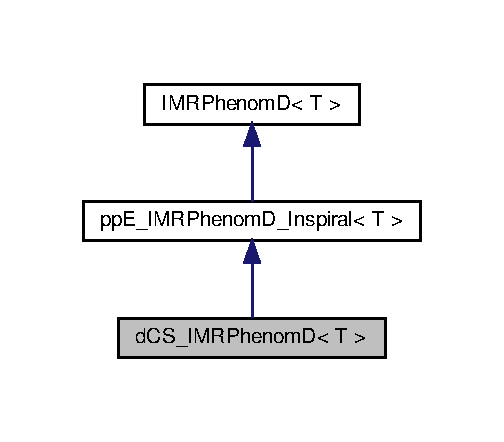
\includegraphics[width=242pt]{classdCS__IMRPhenomD__inherit__graph}
\end{center}
\end{figure}


Collaboration diagram for d\+C\+S\+\_\+\+I\+M\+R\+PhenomD$<$ T $>$\+:
\nopagebreak
\begin{figure}[H]
\begin{center}
\leavevmode
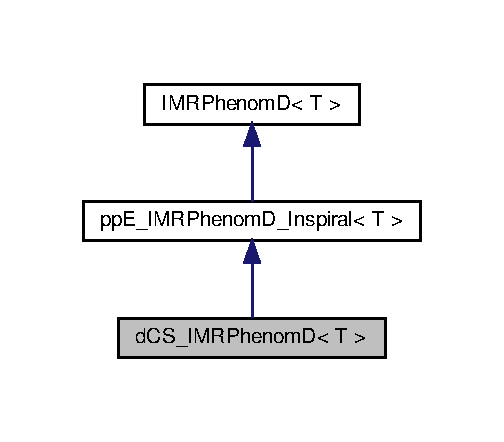
\includegraphics[width=242pt]{classdCS__IMRPhenomD__coll__graph}
\end{center}
\end{figure}
\doxysubsection*{Public Member Functions}
\begin{DoxyCompactItemize}
\item 
virtual int \mbox{\hyperlink{classdCS__IMRPhenomD_ad6fa19d2181da900203c2bf1e182a60b}{construct\+\_\+waveform}} (T $\ast$frequencies, int length, std\+::complex$<$ T $>$ $\ast$waveform, \mbox{\hyperlink{structsource__parameters}{source\+\_\+parameters}}$<$ T $>$ $\ast$params)
\begin{DoxyCompactList}\small\item\em Constructs the waveform as outlined by. \end{DoxyCompactList}\item 
\mbox{\Hypertarget{classdCS__IMRPhenomD_a2325998d0af08e464343d7ae09c085be}\label{classdCS__IMRPhenomD_a2325998d0af08e464343d7ae09c085be}} 
virtual T {\bfseries d\+C\+S\+\_\+phase\+\_\+mod} (\mbox{\hyperlink{structsource__parameters}{source\+\_\+parameters}}$<$ T $>$ $\ast$param)
\item 
\mbox{\Hypertarget{classdCS__IMRPhenomD_ae2aeaa27abdfe564c0e87b20da4a1964}\label{classdCS__IMRPhenomD_ae2aeaa27abdfe564c0e87b20da4a1964}} 
virtual T {\bfseries d\+C\+S\+\_\+phase\+\_\+factor} (\mbox{\hyperlink{structsource__parameters}{source\+\_\+parameters}}$<$ T $>$ $\ast$param)
\item 
virtual int \mbox{\hyperlink{classdCS__IMRPhenomD_ad9dbe0caa4aed7d22b8e6226114ed4d9}{construct\+\_\+amplitude}} (T $\ast$frequencies, int length, T $\ast$amplitude, \mbox{\hyperlink{structsource__parameters}{source\+\_\+parameters}}$<$ T $>$ $\ast$params)
\begin{DoxyCompactList}\small\item\em Constructs the Amplitude as outlined by \mbox{\hyperlink{classIMRPhenomD}{I\+M\+R\+PhenomD}}. \end{DoxyCompactList}\item 
virtual int \mbox{\hyperlink{classdCS__IMRPhenomD_aeee3339b07c8088fc6a1f2c3390f92a4}{construct\+\_\+phase}} (T $\ast$frequencies, int length, T $\ast$phase, \mbox{\hyperlink{structsource__parameters}{source\+\_\+parameters}}$<$ T $>$ $\ast$params)
\begin{DoxyCompactList}\small\item\em Constructs the Phase as outlined by \mbox{\hyperlink{classIMRPhenomD}{I\+M\+R\+PhenomD}}. \end{DoxyCompactList}\end{DoxyCompactItemize}


\doxysubsection{Member Function Documentation}
\mbox{\Hypertarget{classdCS__IMRPhenomD_ad9dbe0caa4aed7d22b8e6226114ed4d9}\label{classdCS__IMRPhenomD_ad9dbe0caa4aed7d22b8e6226114ed4d9}} 
\index{dCS\_IMRPhenomD$<$ T $>$@{dCS\_IMRPhenomD$<$ T $>$}!construct\_amplitude@{construct\_amplitude}}
\index{construct\_amplitude@{construct\_amplitude}!dCS\_IMRPhenomD$<$ T $>$@{dCS\_IMRPhenomD$<$ T $>$}}
\doxysubsubsection{\texorpdfstring{construct\_amplitude()}{construct\_amplitude()}}
{\footnotesize\ttfamily template$<$class T $>$ \\
int \mbox{\hyperlink{classdCS__IMRPhenomD}{d\+C\+S\+\_\+\+I\+M\+R\+PhenomD}}$<$ T $>$\+::construct\+\_\+amplitude (\begin{DoxyParamCaption}\item[{T $\ast$}]{frequencies,  }\item[{int}]{length,  }\item[{T $\ast$}]{amplitude,  }\item[{\mbox{\hyperlink{structsource__parameters}{source\+\_\+parameters}}$<$ T $>$ $\ast$}]{params }\end{DoxyParamCaption})\hspace{0.3cm}{\ttfamily [virtual]}}



Constructs the Amplitude as outlined by \mbox{\hyperlink{classIMRPhenomD}{I\+M\+R\+PhenomD}}. 

arguments\+: array of frequencies, length of that array, T array for the output amplitude, and a \mbox{\hyperlink{structsource__parameters}{source\+\_\+parameters}} structure 
\begin{DoxyParams}{Parameters}
{\em frequencies} & T array of frequencies the waveform is to be evaulated at \\
\hline
{\em length} & integer length of the input array of frequencies and the output array \\
\hline
{\em amplitude} & output T array for the amplitude \\
\hline
{\em params} & Structure of source parameters to be initilized before computation \\
\hline
\end{DoxyParams}


Reimplemented from \mbox{\hyperlink{classIMRPhenomD_a95e7946061fa24fdb7a770dba02147be}{I\+M\+R\+Phenom\+D$<$ T $>$}}.

\mbox{\Hypertarget{classdCS__IMRPhenomD_aeee3339b07c8088fc6a1f2c3390f92a4}\label{classdCS__IMRPhenomD_aeee3339b07c8088fc6a1f2c3390f92a4}} 
\index{dCS\_IMRPhenomD$<$ T $>$@{dCS\_IMRPhenomD$<$ T $>$}!construct\_phase@{construct\_phase}}
\index{construct\_phase@{construct\_phase}!dCS\_IMRPhenomD$<$ T $>$@{dCS\_IMRPhenomD$<$ T $>$}}
\doxysubsubsection{\texorpdfstring{construct\_phase()}{construct\_phase()}}
{\footnotesize\ttfamily template$<$class T $>$ \\
int \mbox{\hyperlink{classdCS__IMRPhenomD}{d\+C\+S\+\_\+\+I\+M\+R\+PhenomD}}$<$ T $>$\+::construct\+\_\+phase (\begin{DoxyParamCaption}\item[{T $\ast$}]{frequencies,  }\item[{int}]{length,  }\item[{T $\ast$}]{phase,  }\item[{\mbox{\hyperlink{structsource__parameters}{source\+\_\+parameters}}$<$ T $>$ $\ast$}]{params }\end{DoxyParamCaption})\hspace{0.3cm}{\ttfamily [virtual]}}



Constructs the Phase as outlined by \mbox{\hyperlink{classIMRPhenomD}{I\+M\+R\+PhenomD}}. 

arguments\+: array of frequencies, length of that array, T array for the output phase, and a \mbox{\hyperlink{structsource__parameters}{source\+\_\+parameters}} structure 
\begin{DoxyParams}{Parameters}
{\em frequencies} & T array of frequencies the waveform is to be evaluated at \\
\hline
{\em length} & integer length of the input and output arrays \\
\hline
{\em phase} & output T array for the phasee \\
\hline
{\em params} & structure of source parameters to be calculated before computation \\
\hline
\end{DoxyParams}


Reimplemented from \mbox{\hyperlink{classIMRPhenomD_abcbaafd0dc4086d2abe1f5ce256908c2}{I\+M\+R\+Phenom\+D$<$ T $>$}}.

\mbox{\Hypertarget{classdCS__IMRPhenomD_ad6fa19d2181da900203c2bf1e182a60b}\label{classdCS__IMRPhenomD_ad6fa19d2181da900203c2bf1e182a60b}} 
\index{dCS\_IMRPhenomD$<$ T $>$@{dCS\_IMRPhenomD$<$ T $>$}!construct\_waveform@{construct\_waveform}}
\index{construct\_waveform@{construct\_waveform}!dCS\_IMRPhenomD$<$ T $>$@{dCS\_IMRPhenomD$<$ T $>$}}
\doxysubsubsection{\texorpdfstring{construct\_waveform()}{construct\_waveform()}}
{\footnotesize\ttfamily template$<$class T $>$ \\
int \mbox{\hyperlink{classdCS__IMRPhenomD}{d\+C\+S\+\_\+\+I\+M\+R\+PhenomD}}$<$ T $>$\+::construct\+\_\+waveform (\begin{DoxyParamCaption}\item[{T $\ast$}]{frequencies,  }\item[{int}]{length,  }\item[{std\+::complex$<$ T $>$ $\ast$}]{waveform,  }\item[{\mbox{\hyperlink{structsource__parameters}{source\+\_\+parameters}}$<$ T $>$ $\ast$}]{params }\end{DoxyParamCaption})\hspace{0.3cm}{\ttfamily [virtual]}}



Constructs the waveform as outlined by. 

arguments\+: array of frequencies, length of that array, a complex array for the output waveform, and a \mbox{\hyperlink{structsource__parameters}{source\+\_\+parameters}} structure 
\begin{DoxyParams}{Parameters}
{\em frequencies} & T array of frequencies the waveform is to be evaluated at \\
\hline
{\em length} & integer length of the array of frequencies and the waveform \\
\hline
{\em waveform} & complex T array for the waveform to be output \\
\hline
\end{DoxyParams}


Reimplemented from \mbox{\hyperlink{classIMRPhenomD_aa7192bf99437b49e0b4f27a342a79dae}{I\+M\+R\+Phenom\+D$<$ T $>$}}.



The documentation for this class was generated from the following files\+:\begin{DoxyCompactItemize}
\item 
include/gwat/\mbox{\hyperlink{ppE__IMRPhenomD_8h}{pp\+E\+\_\+\+I\+M\+R\+Phenom\+D.\+h}}\item 
src/\mbox{\hyperlink{ppE__IMRPhenomD_8cpp}{pp\+E\+\_\+\+I\+M\+R\+Phenom\+D.\+cpp}}\end{DoxyCompactItemize}

\hypertarget{classdCS__IMRPhenomD__log}{}\section{d\+C\+S\+\_\+\+I\+M\+R\+Phenom\+D\+\_\+log$<$ T $>$ Class Template Reference}
\label{classdCS__IMRPhenomD__log}\index{d\+C\+S\+\_\+\+I\+M\+R\+Phenom\+D\+\_\+log$<$ T $>$@{d\+C\+S\+\_\+\+I\+M\+R\+Phenom\+D\+\_\+log$<$ T $>$}}


Inheritance diagram for d\+C\+S\+\_\+\+I\+M\+R\+Phenom\+D\+\_\+log$<$ T $>$\+:\nopagebreak
\begin{figure}[H]
\begin{center}
\leavevmode
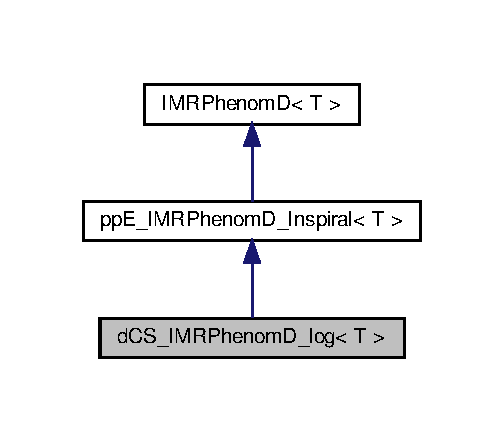
\includegraphics[width=242pt]{classdCS__IMRPhenomD__log__inherit__graph}
\end{center}
\end{figure}


Collaboration diagram for d\+C\+S\+\_\+\+I\+M\+R\+Phenom\+D\+\_\+log$<$ T $>$\+:\nopagebreak
\begin{figure}[H]
\begin{center}
\leavevmode
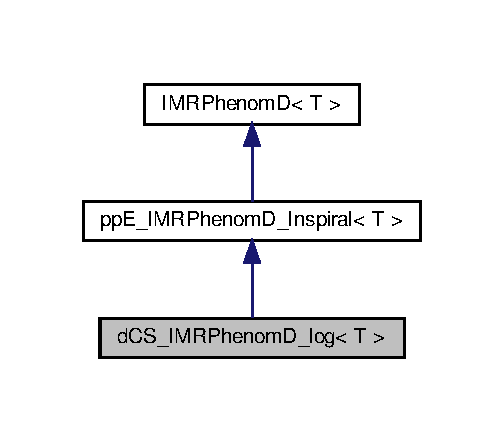
\includegraphics[width=242pt]{classdCS__IMRPhenomD__log__coll__graph}
\end{center}
\end{figure}
\subsection*{Public Member Functions}
\begin{DoxyCompactItemize}
\item 
virtual int \hyperlink{classdCS__IMRPhenomD__log_a15ecc7dbe3cf829ac2b2067060aef0c2}{construct\+\_\+waveform} (T $\ast$frequencies, int length, std\+::complex$<$ T $>$ $\ast$waveform, \hyperlink{structsource__parameters}{source\+\_\+parameters}$<$ T $>$ $\ast$params)
\begin{DoxyCompactList}\small\item\em Constructs the waveform as outlined by. \end{DoxyCompactList}\item 
\mbox{\Hypertarget{classdCS__IMRPhenomD__log_aeb35c3795b437195028551ff89029b3b}\label{classdCS__IMRPhenomD__log_aeb35c3795b437195028551ff89029b3b}} 
virtual T {\bfseries d\+C\+S\+\_\+phase\+\_\+mod} (\hyperlink{structsource__parameters}{source\+\_\+parameters}$<$ T $>$ $\ast$param)
\item 
\mbox{\Hypertarget{classdCS__IMRPhenomD__log_a6a8654bb3f33f51744819599766d6087}\label{classdCS__IMRPhenomD__log_a6a8654bb3f33f51744819599766d6087}} 
virtual T {\bfseries d\+C\+S\+\_\+phase\+\_\+factor} (\hyperlink{structsource__parameters}{source\+\_\+parameters}$<$ T $>$ $\ast$param)
\item 
virtual int \hyperlink{classdCS__IMRPhenomD__log_a769498326cbe7738a855fc93201f6e6a}{construct\+\_\+amplitude} (T $\ast$frequencies, int length, T $\ast$amplitude, \hyperlink{structsource__parameters}{source\+\_\+parameters}$<$ T $>$ $\ast$params)
\begin{DoxyCompactList}\small\item\em Constructs the Amplitude as outlined by \hyperlink{classIMRPhenomD}{I\+M\+R\+PhenomD}. \end{DoxyCompactList}\item 
virtual int \hyperlink{classdCS__IMRPhenomD__log_a6f26f618b1ab6e41ae32eb94fefcc185}{construct\+\_\+phase} (T $\ast$frequencies, int length, T $\ast$phase, \hyperlink{structsource__parameters}{source\+\_\+parameters}$<$ T $>$ $\ast$params)
\begin{DoxyCompactList}\small\item\em Constructs the Phase as outlined by \hyperlink{classIMRPhenomD}{I\+M\+R\+PhenomD}. \end{DoxyCompactList}\end{DoxyCompactItemize}


\subsection{Member Function Documentation}
\mbox{\Hypertarget{classdCS__IMRPhenomD__log_a769498326cbe7738a855fc93201f6e6a}\label{classdCS__IMRPhenomD__log_a769498326cbe7738a855fc93201f6e6a}} 
\index{d\+C\+S\+\_\+\+I\+M\+R\+Phenom\+D\+\_\+log@{d\+C\+S\+\_\+\+I\+M\+R\+Phenom\+D\+\_\+log}!construct\+\_\+amplitude@{construct\+\_\+amplitude}}
\index{construct\+\_\+amplitude@{construct\+\_\+amplitude}!d\+C\+S\+\_\+\+I\+M\+R\+Phenom\+D\+\_\+log@{d\+C\+S\+\_\+\+I\+M\+R\+Phenom\+D\+\_\+log}}
\subsubsection{\texorpdfstring{construct\+\_\+amplitude()}{construct\_amplitude()}}
{\footnotesize\ttfamily template$<$class T $>$ \\
int \hyperlink{classdCS__IMRPhenomD__log}{d\+C\+S\+\_\+\+I\+M\+R\+Phenom\+D\+\_\+log}$<$ T $>$\+::construct\+\_\+amplitude (\begin{DoxyParamCaption}\item[{T $\ast$}]{frequencies,  }\item[{int}]{length,  }\item[{T $\ast$}]{amplitude,  }\item[{\hyperlink{structsource__parameters}{source\+\_\+parameters}$<$ T $>$ $\ast$}]{params }\end{DoxyParamCaption})\hspace{0.3cm}{\ttfamily [virtual]}}



Constructs the Amplitude as outlined by \hyperlink{classIMRPhenomD}{I\+M\+R\+PhenomD}. 

arguments\+: array of frequencies, length of that array, T array for the output amplitude, and a \hyperlink{structsource__parameters}{source\+\_\+parameters} structure 

Reimplemented from \hyperlink{classIMRPhenomD_a95e7946061fa24fdb7a770dba02147be}{I\+M\+R\+Phenom\+D$<$ T $>$}.

\mbox{\Hypertarget{classdCS__IMRPhenomD__log_a6f26f618b1ab6e41ae32eb94fefcc185}\label{classdCS__IMRPhenomD__log_a6f26f618b1ab6e41ae32eb94fefcc185}} 
\index{d\+C\+S\+\_\+\+I\+M\+R\+Phenom\+D\+\_\+log@{d\+C\+S\+\_\+\+I\+M\+R\+Phenom\+D\+\_\+log}!construct\+\_\+phase@{construct\+\_\+phase}}
\index{construct\+\_\+phase@{construct\+\_\+phase}!d\+C\+S\+\_\+\+I\+M\+R\+Phenom\+D\+\_\+log@{d\+C\+S\+\_\+\+I\+M\+R\+Phenom\+D\+\_\+log}}
\subsubsection{\texorpdfstring{construct\+\_\+phase()}{construct\_phase()}}
{\footnotesize\ttfamily template$<$class T $>$ \\
int \hyperlink{classdCS__IMRPhenomD__log}{d\+C\+S\+\_\+\+I\+M\+R\+Phenom\+D\+\_\+log}$<$ T $>$\+::construct\+\_\+phase (\begin{DoxyParamCaption}\item[{T $\ast$}]{frequencies,  }\item[{int}]{length,  }\item[{T $\ast$}]{phase,  }\item[{\hyperlink{structsource__parameters}{source\+\_\+parameters}$<$ T $>$ $\ast$}]{params }\end{DoxyParamCaption})\hspace{0.3cm}{\ttfamily [virtual]}}



Constructs the Phase as outlined by \hyperlink{classIMRPhenomD}{I\+M\+R\+PhenomD}. 

arguments\+: array of frequencies, length of that array, T array for the output phase, and a \hyperlink{structsource__parameters}{source\+\_\+parameters} structure 

Reimplemented from \hyperlink{classIMRPhenomD_abcbaafd0dc4086d2abe1f5ce256908c2}{I\+M\+R\+Phenom\+D$<$ T $>$}.

\mbox{\Hypertarget{classdCS__IMRPhenomD__log_a15ecc7dbe3cf829ac2b2067060aef0c2}\label{classdCS__IMRPhenomD__log_a15ecc7dbe3cf829ac2b2067060aef0c2}} 
\index{d\+C\+S\+\_\+\+I\+M\+R\+Phenom\+D\+\_\+log@{d\+C\+S\+\_\+\+I\+M\+R\+Phenom\+D\+\_\+log}!construct\+\_\+waveform@{construct\+\_\+waveform}}
\index{construct\+\_\+waveform@{construct\+\_\+waveform}!d\+C\+S\+\_\+\+I\+M\+R\+Phenom\+D\+\_\+log@{d\+C\+S\+\_\+\+I\+M\+R\+Phenom\+D\+\_\+log}}
\subsubsection{\texorpdfstring{construct\+\_\+waveform()}{construct\_waveform()}}
{\footnotesize\ttfamily template$<$class T $>$ \\
int \hyperlink{classdCS__IMRPhenomD__log}{d\+C\+S\+\_\+\+I\+M\+R\+Phenom\+D\+\_\+log}$<$ T $>$\+::construct\+\_\+waveform (\begin{DoxyParamCaption}\item[{T $\ast$}]{frequencies,  }\item[{int}]{length,  }\item[{std\+::complex$<$ T $>$ $\ast$}]{waveform,  }\item[{\hyperlink{structsource__parameters}{source\+\_\+parameters}$<$ T $>$ $\ast$}]{params }\end{DoxyParamCaption})\hspace{0.3cm}{\ttfamily [virtual]}}



Constructs the waveform as outlined by. 

arguments\+: array of frequencies, length of that array, a complex array for the output waveform, and a \hyperlink{structsource__parameters}{source\+\_\+parameters} structure 

Reimplemented from \hyperlink{classIMRPhenomD_aa7192bf99437b49e0b4f27a342a79dae}{I\+M\+R\+Phenom\+D$<$ T $>$}.



The documentation for this class was generated from the following files\+:\begin{DoxyCompactItemize}
\item 
include/gwat/\hyperlink{ppE__IMRPhenomD_8h}{pp\+E\+\_\+\+I\+M\+R\+Phenom\+D.\+h}\item 
src/\hyperlink{ppE__IMRPhenomD_8cpp}{pp\+E\+\_\+\+I\+M\+R\+Phenom\+D.\+cpp}\end{DoxyCompactItemize}

\hypertarget{classdefault__comp}{}\doxysection{default\+\_\+comp$<$ jobtype $>$ Class Template Reference}
\label{classdefault__comp}\index{default\_comp$<$ jobtype $>$@{default\_comp$<$ jobtype $>$}}


Default comparator for priority\+\_\+queue in \mbox{\hyperlink{classthreadPool}{thread\+Pool}} -- no comparison.  




{\ttfamily \#include $<$thread\+Pool.\+h$>$}

\doxysubsection*{Public Member Functions}
\begin{DoxyCompactItemize}
\item 
\mbox{\Hypertarget{classdefault__comp_a196f2629bf071bb72fcbbd2454ca628e}\label{classdefault__comp_a196f2629bf071bb72fcbbd2454ca628e}} 
bool {\bfseries operator()} (jobtype j, jobtype k)
\end{DoxyCompactItemize}


\doxysubsection{Detailed Description}
\subsubsection*{template$<$class jobtype$>$\newline
class default\+\_\+comp$<$ jobtype $>$}

Default comparator for priority\+\_\+queue in \mbox{\hyperlink{classthreadPool}{thread\+Pool}} -- no comparison. 

First in first out, not sorting 

The documentation for this class was generated from the following file\+:\begin{DoxyCompactItemize}
\item 
include/gwat/\mbox{\hyperlink{threadPool_8h}{thread\+Pool.\+h}}\end{DoxyCompactItemize}

\hypertarget{classEdGB__IMRPhenomD}{}\doxysection{Ed\+G\+B\+\_\+\+I\+M\+R\+PhenomD$<$ T $>$ Class Template Reference}
\label{classEdGB__IMRPhenomD}\index{EdGB\_IMRPhenomD$<$ T $>$@{EdGB\_IMRPhenomD$<$ T $>$}}


Inheritance diagram for Ed\+G\+B\+\_\+\+I\+M\+R\+PhenomD$<$ T $>$\+:
% FIG 0


Collaboration diagram for Ed\+G\+B\+\_\+\+I\+M\+R\+PhenomD$<$ T $>$\+:
% FIG 1
\doxysubsection*{Public Member Functions}
\begin{DoxyCompactItemize}
\item 
virtual int \mbox{\hyperlink{classEdGB__IMRPhenomD_a11f86d5239ced2ab1372375cd930f12c}{construct\+\_\+waveform}} (T $\ast$frequencies, int length, std\+::complex$<$ T $>$ $\ast$waveform, \mbox{\hyperlink{structsource__parameters}{source\+\_\+parameters}}$<$ T $>$ $\ast$params)
\begin{DoxyCompactList}\small\item\em Constructs the waveform as outlined by. \end{DoxyCompactList}\item 
\mbox{\Hypertarget{classEdGB__IMRPhenomD_a033e2181401b6c440bfabd3a2b16d42a}\label{classEdGB__IMRPhenomD_a033e2181401b6c440bfabd3a2b16d42a}} 
virtual T {\bfseries Ed\+G\+B\+\_\+phase\+\_\+mod} (\mbox{\hyperlink{structsource__parameters}{source\+\_\+parameters}}$<$ T $>$ $\ast$param)
\item 
\mbox{\Hypertarget{classEdGB__IMRPhenomD_a3f0d31deb796dc11c00c36caa21cfc25}\label{classEdGB__IMRPhenomD_a3f0d31deb796dc11c00c36caa21cfc25}} 
virtual T {\bfseries Ed\+G\+B\+\_\+phase\+\_\+factor} (\mbox{\hyperlink{structsource__parameters}{source\+\_\+parameters}}$<$ T $>$ $\ast$param)
\item 
virtual int \mbox{\hyperlink{classEdGB__IMRPhenomD_ae845acb1900b80ce6b23952939f64f2a}{construct\+\_\+amplitude}} (T $\ast$frequencies, int length, T $\ast$amplitude, \mbox{\hyperlink{structsource__parameters}{source\+\_\+parameters}}$<$ T $>$ $\ast$params)
\begin{DoxyCompactList}\small\item\em Constructs the Amplitude as outlined by \mbox{\hyperlink{classIMRPhenomD}{I\+M\+R\+PhenomD}}. \end{DoxyCompactList}\item 
virtual int \mbox{\hyperlink{classEdGB__IMRPhenomD_ad4a5d858678d07912f43e8a045f5979b}{construct\+\_\+phase}} (T $\ast$frequencies, int length, T $\ast$phase, \mbox{\hyperlink{structsource__parameters}{source\+\_\+parameters}}$<$ T $>$ $\ast$params)
\begin{DoxyCompactList}\small\item\em Constructs the Phase as outlined by \mbox{\hyperlink{classIMRPhenomD}{I\+M\+R\+PhenomD}}. \end{DoxyCompactList}\end{DoxyCompactItemize}


\doxysubsection{Member Function Documentation}
\mbox{\Hypertarget{classEdGB__IMRPhenomD_ae845acb1900b80ce6b23952939f64f2a}\label{classEdGB__IMRPhenomD_ae845acb1900b80ce6b23952939f64f2a}} 
\index{EdGB\_IMRPhenomD$<$ T $>$@{EdGB\_IMRPhenomD$<$ T $>$}!construct\_amplitude@{construct\_amplitude}}
\index{construct\_amplitude@{construct\_amplitude}!EdGB\_IMRPhenomD$<$ T $>$@{EdGB\_IMRPhenomD$<$ T $>$}}
\doxysubsubsection{\texorpdfstring{construct\_amplitude()}{construct\_amplitude()}}
{\footnotesize\ttfamily template$<$class T $>$ \\
int \mbox{\hyperlink{classEdGB__IMRPhenomD}{Ed\+G\+B\+\_\+\+I\+M\+R\+PhenomD}}$<$ T $>$\+::construct\+\_\+amplitude (\begin{DoxyParamCaption}\item[{T $\ast$}]{frequencies,  }\item[{int}]{length,  }\item[{T $\ast$}]{amplitude,  }\item[{\mbox{\hyperlink{structsource__parameters}{source\+\_\+parameters}}$<$ T $>$ $\ast$}]{params }\end{DoxyParamCaption})\hspace{0.3cm}{\ttfamily [virtual]}}



Constructs the Amplitude as outlined by \mbox{\hyperlink{classIMRPhenomD}{I\+M\+R\+PhenomD}}. 

arguments\+: array of frequencies, length of that array, T array for the output amplitude, and a \mbox{\hyperlink{structsource__parameters}{source\+\_\+parameters}} structure 
\begin{DoxyParams}{Parameters}
{\em frequencies} & T array of frequencies the waveform is to be evaulated at \\
\hline
{\em length} & integer length of the input array of frequencies and the output array \\
\hline
{\em amplitude} & output T array for the amplitude \\
\hline
{\em params} & Structure of source parameters to be initilized before computation \\
\hline
\end{DoxyParams}


Reimplemented from \mbox{\hyperlink{classIMRPhenomD_a95e7946061fa24fdb7a770dba02147be}{I\+M\+R\+Phenom\+D$<$ T $>$}}.

\mbox{\Hypertarget{classEdGB__IMRPhenomD_ad4a5d858678d07912f43e8a045f5979b}\label{classEdGB__IMRPhenomD_ad4a5d858678d07912f43e8a045f5979b}} 
\index{EdGB\_IMRPhenomD$<$ T $>$@{EdGB\_IMRPhenomD$<$ T $>$}!construct\_phase@{construct\_phase}}
\index{construct\_phase@{construct\_phase}!EdGB\_IMRPhenomD$<$ T $>$@{EdGB\_IMRPhenomD$<$ T $>$}}
\doxysubsubsection{\texorpdfstring{construct\_phase()}{construct\_phase()}}
{\footnotesize\ttfamily template$<$class T $>$ \\
int \mbox{\hyperlink{classEdGB__IMRPhenomD}{Ed\+G\+B\+\_\+\+I\+M\+R\+PhenomD}}$<$ T $>$\+::construct\+\_\+phase (\begin{DoxyParamCaption}\item[{T $\ast$}]{frequencies,  }\item[{int}]{length,  }\item[{T $\ast$}]{phase,  }\item[{\mbox{\hyperlink{structsource__parameters}{source\+\_\+parameters}}$<$ T $>$ $\ast$}]{params }\end{DoxyParamCaption})\hspace{0.3cm}{\ttfamily [virtual]}}



Constructs the Phase as outlined by \mbox{\hyperlink{classIMRPhenomD}{I\+M\+R\+PhenomD}}. 

arguments\+: array of frequencies, length of that array, T array for the output phase, and a \mbox{\hyperlink{structsource__parameters}{source\+\_\+parameters}} structure 
\begin{DoxyParams}{Parameters}
{\em frequencies} & T array of frequencies the waveform is to be evaluated at \\
\hline
{\em length} & integer length of the input and output arrays \\
\hline
{\em phase} & output T array for the phasee \\
\hline
{\em params} & structure of source parameters to be calculated before computation \\
\hline
\end{DoxyParams}


Reimplemented from \mbox{\hyperlink{classIMRPhenomD_abcbaafd0dc4086d2abe1f5ce256908c2}{I\+M\+R\+Phenom\+D$<$ T $>$}}.

\mbox{\Hypertarget{classEdGB__IMRPhenomD_a11f86d5239ced2ab1372375cd930f12c}\label{classEdGB__IMRPhenomD_a11f86d5239ced2ab1372375cd930f12c}} 
\index{EdGB\_IMRPhenomD$<$ T $>$@{EdGB\_IMRPhenomD$<$ T $>$}!construct\_waveform@{construct\_waveform}}
\index{construct\_waveform@{construct\_waveform}!EdGB\_IMRPhenomD$<$ T $>$@{EdGB\_IMRPhenomD$<$ T $>$}}
\doxysubsubsection{\texorpdfstring{construct\_waveform()}{construct\_waveform()}}
{\footnotesize\ttfamily template$<$class T $>$ \\
int \mbox{\hyperlink{classEdGB__IMRPhenomD}{Ed\+G\+B\+\_\+\+I\+M\+R\+PhenomD}}$<$ T $>$\+::construct\+\_\+waveform (\begin{DoxyParamCaption}\item[{T $\ast$}]{frequencies,  }\item[{int}]{length,  }\item[{std\+::complex$<$ T $>$ $\ast$}]{waveform,  }\item[{\mbox{\hyperlink{structsource__parameters}{source\+\_\+parameters}}$<$ T $>$ $\ast$}]{params }\end{DoxyParamCaption})\hspace{0.3cm}{\ttfamily [virtual]}}



Constructs the waveform as outlined by. 

arguments\+: array of frequencies, length of that array, a complex array for the output waveform, and a \mbox{\hyperlink{structsource__parameters}{source\+\_\+parameters}} structure 
\begin{DoxyParams}{Parameters}
{\em frequencies} & T array of frequencies the waveform is to be evaluated at \\
\hline
{\em length} & integer length of the array of frequencies and the waveform \\
\hline
{\em waveform} & complex T array for the waveform to be output \\
\hline
\end{DoxyParams}


Reimplemented from \mbox{\hyperlink{classIMRPhenomD_aa7192bf99437b49e0b4f27a342a79dae}{I\+M\+R\+Phenom\+D$<$ T $>$}}.



The documentation for this class was generated from the following files\+:\begin{DoxyCompactItemize}
\item 
include/gwat/\mbox{\hyperlink{ppE__IMRPhenomD_8h}{pp\+E\+\_\+\+I\+M\+R\+Phenom\+D.\+h}}\item 
src/\mbox{\hyperlink{ppE__IMRPhenomD_8cpp}{pp\+E\+\_\+\+I\+M\+R\+Phenom\+D.\+cpp}}\end{DoxyCompactItemize}

\hypertarget{classEdGB__IMRPhenomD__log}{}\doxysection{Ed\+G\+B\+\_\+\+I\+M\+R\+Phenom\+D\+\_\+log$<$ T $>$ Class Template Reference}
\label{classEdGB__IMRPhenomD__log}\index{EdGB\_IMRPhenomD\_log$<$ T $>$@{EdGB\_IMRPhenomD\_log$<$ T $>$}}


Inheritance diagram for Ed\+G\+B\+\_\+\+I\+M\+R\+Phenom\+D\+\_\+log$<$ T $>$\+:
% FIG 0


Collaboration diagram for Ed\+G\+B\+\_\+\+I\+M\+R\+Phenom\+D\+\_\+log$<$ T $>$\+:
% FIG 1
\doxysubsection*{Public Member Functions}
\begin{DoxyCompactItemize}
\item 
virtual int \mbox{\hyperlink{classEdGB__IMRPhenomD__log_afbb021b8af2b53b51ca24d7c29c0d487}{construct\+\_\+waveform}} (T $\ast$frequencies, int length, std\+::complex$<$ T $>$ $\ast$waveform, \mbox{\hyperlink{structsource__parameters}{source\+\_\+parameters}}$<$ T $>$ $\ast$params)
\begin{DoxyCompactList}\small\item\em Constructs the waveform as outlined by. \end{DoxyCompactList}\item 
\mbox{\Hypertarget{classEdGB__IMRPhenomD__log_a79bb77d3ca14ef95ea54026556ede906}\label{classEdGB__IMRPhenomD__log_a79bb77d3ca14ef95ea54026556ede906}} 
virtual T {\bfseries Ed\+G\+B\+\_\+phase\+\_\+mod} (\mbox{\hyperlink{structsource__parameters}{source\+\_\+parameters}}$<$ T $>$ $\ast$param)
\item 
\mbox{\Hypertarget{classEdGB__IMRPhenomD__log_a866e031a86d736e7fc88beb987cd41e8}\label{classEdGB__IMRPhenomD__log_a866e031a86d736e7fc88beb987cd41e8}} 
virtual T {\bfseries Ed\+G\+B\+\_\+phase\+\_\+factor} (\mbox{\hyperlink{structsource__parameters}{source\+\_\+parameters}}$<$ T $>$ $\ast$param)
\item 
virtual int \mbox{\hyperlink{classEdGB__IMRPhenomD__log_ac6acdf1b0231e33b861202bcd9c51ee7}{construct\+\_\+amplitude}} (T $\ast$frequencies, int length, T $\ast$amplitude, \mbox{\hyperlink{structsource__parameters}{source\+\_\+parameters}}$<$ T $>$ $\ast$params)
\begin{DoxyCompactList}\small\item\em Constructs the Amplitude as outlined by \mbox{\hyperlink{classIMRPhenomD}{I\+M\+R\+PhenomD}}. \end{DoxyCompactList}\item 
virtual int \mbox{\hyperlink{classEdGB__IMRPhenomD__log_a62aa82aaadc4210d09e95f8807f8f3c4}{construct\+\_\+phase}} (T $\ast$frequencies, int length, T $\ast$phase, \mbox{\hyperlink{structsource__parameters}{source\+\_\+parameters}}$<$ T $>$ $\ast$params)
\begin{DoxyCompactList}\small\item\em Constructs the Phase as outlined by \mbox{\hyperlink{classIMRPhenomD}{I\+M\+R\+PhenomD}}. \end{DoxyCompactList}\end{DoxyCompactItemize}


\doxysubsection{Member Function Documentation}
\mbox{\Hypertarget{classEdGB__IMRPhenomD__log_ac6acdf1b0231e33b861202bcd9c51ee7}\label{classEdGB__IMRPhenomD__log_ac6acdf1b0231e33b861202bcd9c51ee7}} 
\index{EdGB\_IMRPhenomD\_log$<$ T $>$@{EdGB\_IMRPhenomD\_log$<$ T $>$}!construct\_amplitude@{construct\_amplitude}}
\index{construct\_amplitude@{construct\_amplitude}!EdGB\_IMRPhenomD\_log$<$ T $>$@{EdGB\_IMRPhenomD\_log$<$ T $>$}}
\doxysubsubsection{\texorpdfstring{construct\_amplitude()}{construct\_amplitude()}}
{\footnotesize\ttfamily template$<$class T $>$ \\
int \mbox{\hyperlink{classEdGB__IMRPhenomD__log}{Ed\+G\+B\+\_\+\+I\+M\+R\+Phenom\+D\+\_\+log}}$<$ T $>$\+::construct\+\_\+amplitude (\begin{DoxyParamCaption}\item[{T $\ast$}]{frequencies,  }\item[{int}]{length,  }\item[{T $\ast$}]{amplitude,  }\item[{\mbox{\hyperlink{structsource__parameters}{source\+\_\+parameters}}$<$ T $>$ $\ast$}]{params }\end{DoxyParamCaption})\hspace{0.3cm}{\ttfamily [virtual]}}



Constructs the Amplitude as outlined by \mbox{\hyperlink{classIMRPhenomD}{I\+M\+R\+PhenomD}}. 

arguments\+: array of frequencies, length of that array, T array for the output amplitude, and a \mbox{\hyperlink{structsource__parameters}{source\+\_\+parameters}} structure 
\begin{DoxyParams}{Parameters}
{\em frequencies} & T array of frequencies the waveform is to be evaulated at \\
\hline
{\em length} & integer length of the input array of frequencies and the output array \\
\hline
{\em amplitude} & output T array for the amplitude \\
\hline
{\em params} & Structure of source parameters to be initilized before computation \\
\hline
\end{DoxyParams}


Reimplemented from \mbox{\hyperlink{classIMRPhenomD_a95e7946061fa24fdb7a770dba02147be}{I\+M\+R\+Phenom\+D$<$ T $>$}}.

\mbox{\Hypertarget{classEdGB__IMRPhenomD__log_a62aa82aaadc4210d09e95f8807f8f3c4}\label{classEdGB__IMRPhenomD__log_a62aa82aaadc4210d09e95f8807f8f3c4}} 
\index{EdGB\_IMRPhenomD\_log$<$ T $>$@{EdGB\_IMRPhenomD\_log$<$ T $>$}!construct\_phase@{construct\_phase}}
\index{construct\_phase@{construct\_phase}!EdGB\_IMRPhenomD\_log$<$ T $>$@{EdGB\_IMRPhenomD\_log$<$ T $>$}}
\doxysubsubsection{\texorpdfstring{construct\_phase()}{construct\_phase()}}
{\footnotesize\ttfamily template$<$class T $>$ \\
int \mbox{\hyperlink{classEdGB__IMRPhenomD__log}{Ed\+G\+B\+\_\+\+I\+M\+R\+Phenom\+D\+\_\+log}}$<$ T $>$\+::construct\+\_\+phase (\begin{DoxyParamCaption}\item[{T $\ast$}]{frequencies,  }\item[{int}]{length,  }\item[{T $\ast$}]{phase,  }\item[{\mbox{\hyperlink{structsource__parameters}{source\+\_\+parameters}}$<$ T $>$ $\ast$}]{params }\end{DoxyParamCaption})\hspace{0.3cm}{\ttfamily [virtual]}}



Constructs the Phase as outlined by \mbox{\hyperlink{classIMRPhenomD}{I\+M\+R\+PhenomD}}. 

arguments\+: array of frequencies, length of that array, T array for the output phase, and a \mbox{\hyperlink{structsource__parameters}{source\+\_\+parameters}} structure 
\begin{DoxyParams}{Parameters}
{\em frequencies} & T array of frequencies the waveform is to be evaluated at \\
\hline
{\em length} & integer length of the input and output arrays \\
\hline
{\em phase} & output T array for the phasee \\
\hline
{\em params} & structure of source parameters to be calculated before computation \\
\hline
\end{DoxyParams}


Reimplemented from \mbox{\hyperlink{classIMRPhenomD_abcbaafd0dc4086d2abe1f5ce256908c2}{I\+M\+R\+Phenom\+D$<$ T $>$}}.

\mbox{\Hypertarget{classEdGB__IMRPhenomD__log_afbb021b8af2b53b51ca24d7c29c0d487}\label{classEdGB__IMRPhenomD__log_afbb021b8af2b53b51ca24d7c29c0d487}} 
\index{EdGB\_IMRPhenomD\_log$<$ T $>$@{EdGB\_IMRPhenomD\_log$<$ T $>$}!construct\_waveform@{construct\_waveform}}
\index{construct\_waveform@{construct\_waveform}!EdGB\_IMRPhenomD\_log$<$ T $>$@{EdGB\_IMRPhenomD\_log$<$ T $>$}}
\doxysubsubsection{\texorpdfstring{construct\_waveform()}{construct\_waveform()}}
{\footnotesize\ttfamily template$<$class T $>$ \\
int \mbox{\hyperlink{classEdGB__IMRPhenomD__log}{Ed\+G\+B\+\_\+\+I\+M\+R\+Phenom\+D\+\_\+log}}$<$ T $>$\+::construct\+\_\+waveform (\begin{DoxyParamCaption}\item[{T $\ast$}]{frequencies,  }\item[{int}]{length,  }\item[{std\+::complex$<$ T $>$ $\ast$}]{waveform,  }\item[{\mbox{\hyperlink{structsource__parameters}{source\+\_\+parameters}}$<$ T $>$ $\ast$}]{params }\end{DoxyParamCaption})\hspace{0.3cm}{\ttfamily [virtual]}}



Constructs the waveform as outlined by. 

arguments\+: array of frequencies, length of that array, a complex array for the output waveform, and a \mbox{\hyperlink{structsource__parameters}{source\+\_\+parameters}} structure 
\begin{DoxyParams}{Parameters}
{\em frequencies} & T array of frequencies the waveform is to be evaluated at \\
\hline
{\em length} & integer length of the array of frequencies and the waveform \\
\hline
{\em waveform} & complex T array for the waveform to be output \\
\hline
\end{DoxyParams}


Reimplemented from \mbox{\hyperlink{classIMRPhenomD_aa7192bf99437b49e0b4f27a342a79dae}{I\+M\+R\+Phenom\+D$<$ T $>$}}.



The documentation for this class was generated from the following files\+:\begin{DoxyCompactItemize}
\item 
include/gwat/\mbox{\hyperlink{ppE__IMRPhenomD_8h}{pp\+E\+\_\+\+I\+M\+R\+Phenom\+D.\+h}}\item 
src/\mbox{\hyperlink{ppE__IMRPhenomD_8cpp}{pp\+E\+\_\+\+I\+M\+R\+Phenom\+D.\+cpp}}\end{DoxyCompactItemize}

\hypertarget{structepsilon__coeffs}{}\section{epsilon\+\_\+coeffs$<$ T $>$ Struct Template Reference}
\label{structepsilon__coeffs}\index{epsilon\+\_\+coeffs$<$ T $>$@{epsilon\+\_\+coeffs$<$ T $>$}}
\subsection*{Public Attributes}
\begin{DoxyCompactItemize}
\item 
\mbox{\Hypertarget{structepsilon__coeffs_ab9a930ed682c80d2febd0380480f1eb3}\label{structepsilon__coeffs_ab9a930ed682c80d2febd0380480f1eb3}} 
T {\bfseries coeff1}
\item 
\mbox{\Hypertarget{structepsilon__coeffs_a9ddc676353116186e8abde43522164c5}\label{structepsilon__coeffs_a9ddc676353116186e8abde43522164c5}} 
T {\bfseries coeff2}
\item 
\mbox{\Hypertarget{structepsilon__coeffs_aaaf9c13966c4550d9370d7529eaadfe6}\label{structepsilon__coeffs_aaaf9c13966c4550d9370d7529eaadfe6}} 
T {\bfseries coeff3}
\item 
\mbox{\Hypertarget{structepsilon__coeffs_a87a3c5420d7d0b435fe4e68ee3534b5c}\label{structepsilon__coeffs_a87a3c5420d7d0b435fe4e68ee3534b5c}} 
T {\bfseries coeff4}
\item 
\mbox{\Hypertarget{structepsilon__coeffs_a37f73b1cd1872b4bb54ac86582c5f26b}\label{structepsilon__coeffs_a37f73b1cd1872b4bb54ac86582c5f26b}} 
T {\bfseries coeff5}
\end{DoxyCompactItemize}


The documentation for this struct was generated from the following file\+:\begin{DoxyCompactItemize}
\item 
include/gwat/\hyperlink{IMRPhenomP_8h}{I\+M\+R\+Phenom\+P.\+h}\end{DoxyCompactItemize}

\hypertarget{structfftw__outline}{}\section{fftw\+\_\+outline Struct Reference}
\label{structfftw__outline}\index{fftw\+\_\+outline@{fftw\+\_\+outline}}
\subsection*{Public Attributes}
\begin{DoxyCompactItemize}
\item 
\mbox{\Hypertarget{structfftw__outline_abd3c18149bf7fedd74f18f36f1148a6e}\label{structfftw__outline_abd3c18149bf7fedd74f18f36f1148a6e}} 
fftw\+\_\+complex $\ast$ {\bfseries in}
\item 
\mbox{\Hypertarget{structfftw__outline_a9b52b935e2b3a1ed2a3884842619a152}\label{structfftw__outline_a9b52b935e2b3a1ed2a3884842619a152}} 
fftw\+\_\+complex $\ast$ {\bfseries out}
\item 
\mbox{\Hypertarget{structfftw__outline_a42f638a5f1b1792685c1897c6cb746ef}\label{structfftw__outline_a42f638a5f1b1792685c1897c6cb746ef}} 
fftw\+\_\+plan {\bfseries p}
\end{DoxyCompactItemize}


The documentation for this struct was generated from the following file\+:\begin{DoxyCompactItemize}
\item 
include/gwat/\hyperlink{util_8h}{util.\+h}\end{DoxyCompactItemize}

\hypertarget{classgen__params}{}\doxysection{gen\+\_\+params Class Reference}
\label{classgen__params}\index{gen\_params@{gen\_params}}


convience wrapper for the \mbox{\hyperlink{classgen__params__base}{gen\+\_\+params\+\_\+base}} class  




{\ttfamily \#include $<$util.\+h$>$}



Inheritance diagram for gen\+\_\+params\+:
\nopagebreak
\begin{figure}[H]
\begin{center}
\leavevmode
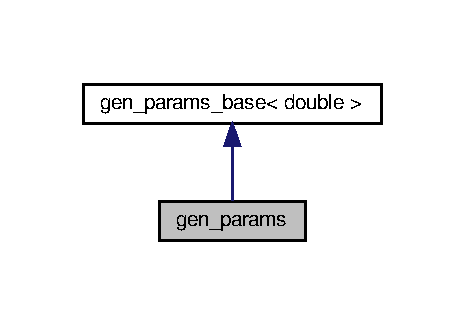
\includegraphics[width=223pt]{classgen__params__inherit__graph}
\end{center}
\end{figure}


Collaboration diagram for gen\+\_\+params\+:
\nopagebreak
\begin{figure}[H]
\begin{center}
\leavevmode
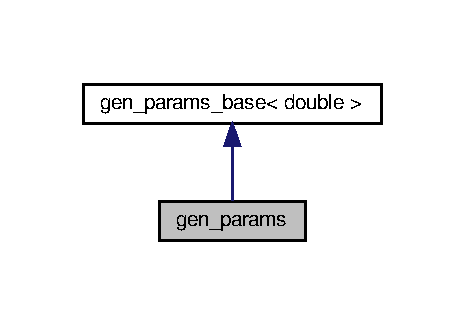
\includegraphics[width=223pt]{classgen__params__coll__graph}
\end{center}
\end{figure}
\doxysubsection*{Additional Inherited Members}


\doxysubsection{Detailed Description}
convience wrapper for the \mbox{\hyperlink{classgen__params__base}{gen\+\_\+params\+\_\+base}} class 

If using the code in the intended way, this is all the user should ever have to use. Just allows the user to drop the template parameter

Also implemented for backwards compatibility with previous versions of the code 

The documentation for this class was generated from the following file\+:\begin{DoxyCompactItemize}
\item 
include/gwat/\mbox{\hyperlink{util_8h}{util.\+h}}\end{DoxyCompactItemize}

\hypertarget{classgen__params__base}{}\section{gen\+\_\+params\+\_\+base$<$ T $>$ Class Template Reference}
\label{classgen__params__base}\index{gen\+\_\+params\+\_\+base$<$ T $>$@{gen\+\_\+params\+\_\+base$<$ T $>$}}


Collaboration diagram for gen\+\_\+params\+\_\+base$<$ T $>$\+:\nopagebreak
\begin{figure}[H]
\begin{center}
\leavevmode
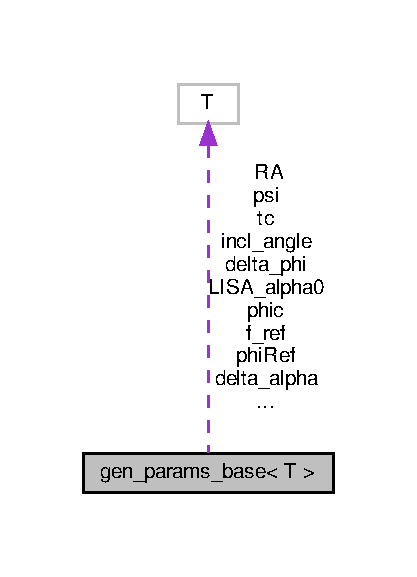
\includegraphics[width=200pt]{classgen__params__base__coll__graph}
\end{center}
\end{figure}
\subsection*{Public Attributes}
\begin{DoxyCompactItemize}
\item 
\mbox{\Hypertarget{classgen__params__base_ae26c1d93a26bb3f7f31b77cefa50b43c}\label{classgen__params__base_ae26c1d93a26bb3f7f31b77cefa50b43c}} 
std\+::string {\bfseries cosmology} =\char`\"{}P\+L\+A\+N\+C\+K15\char`\"{}
\item 
T \hyperlink{classgen__params__base_a8e7626a0841f4d2224b625e327f7679a}{mass1}
\item 
T \hyperlink{classgen__params__base_a8bb568ea6c20f9442a5fd0f1b01344e0}{mass2}
\item 
T \hyperlink{classgen__params__base_ad1fe02f4ddabb07ba1cf42ec7e31d659}{Luminosity\+\_\+\+Distance}
\item 
T \hyperlink{classgen__params__base_a42e83426b899a1b9c987101433943a02}{spin1} \mbox{[}3\mbox{]}
\item 
T \hyperlink{classgen__params__base_a1e8a89670cf689d2b2afc4e59cd89b58}{spin2} \mbox{[}3\mbox{]}
\item 
T \hyperlink{classgen__params__base_a87694ca69c736862b334f3cb6cc82ae6}{tc} =0
\item 
\mbox{\Hypertarget{classgen__params__base_af1c02da522106d065ee3ebefe77a11a6}\label{classgen__params__base_af1c02da522106d065ee3ebefe77a11a6}} 
T {\bfseries psi} =0
\item 
T \hyperlink{classgen__params__base_af55fdc0245e65234b570f5c9918bd88b}{incl\+\_\+angle}
\item 
bool \hyperlink{classgen__params__base_a769d637405f8456595b513305f91d0ca}{equatorial\+\_\+orientation} =false
\item 
T \hyperlink{classgen__params__base_a760b7a0a51b9cd24cb63c13344e6493c}{theta\+\_\+l}
\item 
T \hyperlink{classgen__params__base_aaec5fafce24e74b099b713f47d25045f}{phi\+\_\+l}
\item 
bool \hyperlink{classgen__params__base_a75a9201e603d8d7e348a8ae914b03ee9}{horizon\+\_\+coord} =false
\item 
T \hyperlink{classgen__params__base_a078e76b35c7b95ab24790258ffcc2be0}{theta}
\item 
T \hyperlink{classgen__params__base_a500f71cd641e52356d6371894f7d8a07}{phi}
\item 
T \hyperlink{classgen__params__base_abe5fc4017be70773feba6964cb9616e9}{RA}
\item 
T \hyperlink{classgen__params__base_a1028e164a2ee18b60d4ae902165aefea}{D\+EC}
\item 
double \hyperlink{classgen__params__base_a9cf0459a975c748e8fa828b8af093611}{gmst}
\item 
bool \hyperlink{classgen__params__base_a03398714fe7005a9c80336733c9a2043}{N\+Sflag1} =false
\item 
\mbox{\Hypertarget{classgen__params__base_ad2a4aeb08378293bb6d24e6060fe028f}\label{classgen__params__base_ad2a4aeb08378293bb6d24e6060fe028f}} 
bool {\bfseries N\+Sflag2} =false
\item 
T \hyperlink{classgen__params__base_a8aafd6ccd8331c201bc0f301898d5606}{f\+\_\+ref} =0
\item 
bool \hyperlink{classgen__params__base_adebbc3e4955f322fde2c9ac61f3f61e8}{shift\+\_\+time} = true
\item 
bool \hyperlink{classgen__params__base_a8753041140d91176f966b5f8dfc7de34}{shift\+\_\+phase} = true
\item 
\mbox{\Hypertarget{classgen__params__base_a321a6f0749f80d869c47eba274d8b6ff}\label{classgen__params__base_a321a6f0749f80d869c47eba274d8b6ff}} 
T {\bfseries phi\+Ref} =0
\item 
T \hyperlink{classgen__params__base_a4da02c658f87191c55bb040d5da46143}{phic} =0
\item 
\mbox{\Hypertarget{classgen__params__base_a01109130de63d4105164c732afc6dbd1}\label{classgen__params__base_a01109130de63d4105164c732afc6dbd1}} 
bool {\bfseries sky\+\_\+average} =false
\item 
T \hyperlink{classgen__params__base_ac855eff52f4ec75a63900f63fb8a1942}{theta\+JN} = -\/10
\item 
\mbox{\Hypertarget{classgen__params__base_a4f6b7235552757d42a412693c7490c2f}\label{classgen__params__base_a4f6b7235552757d42a412693c7490c2f}} 
T {\bfseries alpha0} = 0
\item 
\mbox{\Hypertarget{classgen__params__base_a7635c4e8529dd34b2cf1dbd1c706fa21}\label{classgen__params__base_a7635c4e8529dd34b2cf1dbd1c706fa21}} 
T {\bfseries chip} = 0
\item 
\mbox{\Hypertarget{classgen__params__base_a313d4d82fe7474eba59562af31cb20b8}\label{classgen__params__base_a313d4d82fe7474eba59562af31cb20b8}} 
T {\bfseries phip} = -\/1
\item 
\mbox{\Hypertarget{classgen__params__base_ab0d2c6df726cc6118d6a58661e6ac7e8}\label{classgen__params__base_ab0d2c6df726cc6118d6a58661e6ac7e8}} 
bool {\bfseries precess\+\_\+reduced\+\_\+flag} =false
\item 
\mbox{\Hypertarget{classgen__params__base_a62a861a024e7e6d7d9396113c534fd0a}\label{classgen__params__base_a62a861a024e7e6d7d9396113c534fd0a}} 
T {\bfseries L\+I\+S\+A\+\_\+alpha0} =0
\item 
\mbox{\Hypertarget{classgen__params__base_adf1d6bdefba8d888b73f648fc65db9f8}\label{classgen__params__base_adf1d6bdefba8d888b73f648fc65db9f8}} 
T {\bfseries L\+I\+S\+A\+\_\+phi0} =0
\item 
T \hyperlink{classgen__params__base_aa42604158c43f56290551a92316fdce3}{theta\+\_\+j\+\_\+ecl}
\item 
\mbox{\Hypertarget{classgen__params__base_a7cf7b18272c57aa3f07efac05ad8ddd9}\label{classgen__params__base_a7cf7b18272c57aa3f07efac05ad8ddd9}} 
T {\bfseries phi\+\_\+j\+\_\+ecl}
\item 
\mbox{\Hypertarget{classgen__params__base_a35f422810e377c3447e4fd30f9ac1f01}\label{classgen__params__base_a35f422810e377c3447e4fd30f9ac1f01}} 
int {\bfseries Nmod\+\_\+beta} =0
\item 
\mbox{\Hypertarget{classgen__params__base_a0180ee6921241748dd4e567a0989887a}\label{classgen__params__base_a0180ee6921241748dd4e567a0989887a}} 
int {\bfseries Nmod\+\_\+alpha} =0
\item 
\mbox{\Hypertarget{classgen__params__base_aa724b48e72c1aa3fcd249c8468a9bad7}\label{classgen__params__base_aa724b48e72c1aa3fcd249c8468a9bad7}} 
int {\bfseries Nmod\+\_\+sigma} =0
\item 
\mbox{\Hypertarget{classgen__params__base_acd740b871d4bbc6466bc20a0cd1880da}\label{classgen__params__base_acd740b871d4bbc6466bc20a0cd1880da}} 
int {\bfseries Nmod\+\_\+phi} =0
\item 
\mbox{\Hypertarget{classgen__params__base_aa68ac108aa5f23c60c1df48d38344b11}\label{classgen__params__base_aa68ac108aa5f23c60c1df48d38344b11}} 
int $\ast$ {\bfseries betai}
\item 
\mbox{\Hypertarget{classgen__params__base_a8f2b68e50ea5598b897e2d06a4e2d1e7}\label{classgen__params__base_a8f2b68e50ea5598b897e2d06a4e2d1e7}} 
int $\ast$ {\bfseries alphai}
\item 
\mbox{\Hypertarget{classgen__params__base_ac9aec95a0c8f354e20af93ef83257401}\label{classgen__params__base_ac9aec95a0c8f354e20af93ef83257401}} 
int $\ast$ {\bfseries sigmai}
\item 
\mbox{\Hypertarget{classgen__params__base_a6a47aa9b90719251e70da1481acd3ca8}\label{classgen__params__base_a6a47aa9b90719251e70da1481acd3ca8}} 
int $\ast$ {\bfseries phii}
\item 
\mbox{\Hypertarget{classgen__params__base_ab98da87e5508f22224fcabab702e3289}\label{classgen__params__base_ab98da87e5508f22224fcabab702e3289}} 
T $\ast$ {\bfseries delta\+\_\+beta}
\item 
\mbox{\Hypertarget{classgen__params__base_a8018571edb80fabd65d96eab010246f0}\label{classgen__params__base_a8018571edb80fabd65d96eab010246f0}} 
T $\ast$ {\bfseries delta\+\_\+alpha}
\item 
\mbox{\Hypertarget{classgen__params__base_aebab46f2bf055e4f9ae68082d71f5c1a}\label{classgen__params__base_aebab46f2bf055e4f9ae68082d71f5c1a}} 
T $\ast$ {\bfseries delta\+\_\+sigma}
\item 
\mbox{\Hypertarget{classgen__params__base_a282e3598eaf76a2f857726dfef189188}\label{classgen__params__base_a282e3598eaf76a2f857726dfef189188}} 
T $\ast$ {\bfseries delta\+\_\+phi}
\item 
int $\ast$ \hyperlink{classgen__params__base_a6ef4d26715ba4696f2fa60acf9930a41}{bppe}
\item 
T $\ast$ \hyperlink{classgen__params__base_ac0442682283e1e71d8c1410b99f50fe3}{betappe}
\item 
int \hyperlink{classgen__params__base_adce2e842deae1db65c22fbc74cc9b7ed}{Nmod} =0
\item 
\mbox{\Hypertarget{classgen__params__base_a61278889182aeb69be0002db898b1159}\label{classgen__params__base_a61278889182aeb69be0002db898b1159}} 
T {\bfseries chi1\+\_\+l} = 0
\item 
\mbox{\Hypertarget{classgen__params__base_a1dbf7bb37dd195c5f0aee49e24e61392}\label{classgen__params__base_a1dbf7bb37dd195c5f0aee49e24e61392}} 
T {\bfseries chi2\+\_\+l} = 0
\item 
\mbox{\Hypertarget{classgen__params__base_ab37864386335e3df52d0d7beb077d57a}\label{classgen__params__base_ab37864386335e3df52d0d7beb077d57a}} 
T {\bfseries phi\+JL} = 0
\item 
\mbox{\Hypertarget{classgen__params__base_ac177cb6a18c478fb9d8cee26f39c858d}\label{classgen__params__base_ac177cb6a18c478fb9d8cee26f39c858d}} 
T {\bfseries theta\+JL} = 0
\item 
\mbox{\Hypertarget{classgen__params__base_a79fd8f75c600381faed19e2c55897e79}\label{classgen__params__base_a79fd8f75c600381faed19e2c55897e79}} 
T {\bfseries zeta\+\_\+polariz} =0
\item 
\mbox{\Hypertarget{classgen__params__base_a1b6c91991fff3feea67e473e0e6ab448}\label{classgen__params__base_a1b6c91991fff3feea67e473e0e6ab448}} 
T {\bfseries phi\+\_\+aligned} = 0
\item 
\mbox{\Hypertarget{classgen__params__base_a54b56e9532a0b4b6dcb48d2454da7d93}\label{classgen__params__base_a54b56e9532a0b4b6dcb48d2454da7d93}} 
T {\bfseries chil} = 0
\item 
\mbox{\Hypertarget{classgen__params__base_a551ef3f246f186bf3ff1f4b51a40b465}\label{classgen__params__base_a551ef3f246f186bf3ff1f4b51a40b465}} 
gsl\+\_\+spline $\ast$ {\bfseries Z\+\_\+\+D\+L\+\_\+spline\+\_\+ptr} =N\+U\+LL
\item 
\mbox{\Hypertarget{classgen__params__base_aabdb7823d0d6c98a79e6f16c63ceff63}\label{classgen__params__base_aabdb7823d0d6c98a79e6f16c63ceff63}} 
gsl\+\_\+interp\+\_\+accel $\ast$ {\bfseries Z\+\_\+\+D\+L\+\_\+accel\+\_\+ptr} =N\+U\+LL
\end{DoxyCompactItemize}


\subsection{Member Data Documentation}
\mbox{\Hypertarget{classgen__params__base_ac0442682283e1e71d8c1410b99f50fe3}\label{classgen__params__base_ac0442682283e1e71d8c1410b99f50fe3}} 
\index{gen\+\_\+params\+\_\+base@{gen\+\_\+params\+\_\+base}!betappe@{betappe}}
\index{betappe@{betappe}!gen\+\_\+params\+\_\+base@{gen\+\_\+params\+\_\+base}}
\subsubsection{\texorpdfstring{betappe}{betappe}}
{\footnotesize\ttfamily template$<$class T$>$ \\
T$\ast$ \hyperlink{classgen__params__base}{gen\+\_\+params\+\_\+base}$<$ T $>$\+::betappe}

ppE coefficient for the phase modification -\/ vector for multiple modifications \mbox{\Hypertarget{classgen__params__base_a6ef4d26715ba4696f2fa60acf9930a41}\label{classgen__params__base_a6ef4d26715ba4696f2fa60acf9930a41}} 
\index{gen\+\_\+params\+\_\+base@{gen\+\_\+params\+\_\+base}!bppe@{bppe}}
\index{bppe@{bppe}!gen\+\_\+params\+\_\+base@{gen\+\_\+params\+\_\+base}}
\subsubsection{\texorpdfstring{bppe}{bppe}}
{\footnotesize\ttfamily template$<$class T$>$ \\
int$\ast$ \hyperlink{classgen__params__base}{gen\+\_\+params\+\_\+base}$<$ T $>$\+::bppe}

ppE b parameter (power of the frequency) -\/ vector for multiple modifications \mbox{\Hypertarget{classgen__params__base_a1028e164a2ee18b60d4ae902165aefea}\label{classgen__params__base_a1028e164a2ee18b60d4ae902165aefea}} 
\index{gen\+\_\+params\+\_\+base@{gen\+\_\+params\+\_\+base}!D\+EC@{D\+EC}}
\index{D\+EC@{D\+EC}!gen\+\_\+params\+\_\+base@{gen\+\_\+params\+\_\+base}}
\subsubsection{\texorpdfstring{D\+EC}{DEC}}
{\footnotesize\ttfamily template$<$class T$>$ \\
T \hyperlink{classgen__params__base}{gen\+\_\+params\+\_\+base}$<$ T $>$\+::D\+EC}

Equatorial coordinates of source D\+EC \mbox{\Hypertarget{classgen__params__base_a769d637405f8456595b513305f91d0ca}\label{classgen__params__base_a769d637405f8456595b513305f91d0ca}} 
\index{gen\+\_\+params\+\_\+base@{gen\+\_\+params\+\_\+base}!equatorial\+\_\+orientation@{equatorial\+\_\+orientation}}
\index{equatorial\+\_\+orientation@{equatorial\+\_\+orientation}!gen\+\_\+params\+\_\+base@{gen\+\_\+params\+\_\+base}}
\subsubsection{\texorpdfstring{equatorial\+\_\+orientation}{equatorial\_orientation}}
{\footnotesize\ttfamily template$<$class T$>$ \\
bool \hyperlink{classgen__params__base}{gen\+\_\+params\+\_\+base}$<$ T $>$\+::equatorial\+\_\+orientation =false}

boolean flag indicating equatorial orientation coordinates should be used \mbox{\Hypertarget{classgen__params__base_a8aafd6ccd8331c201bc0f301898d5606}\label{classgen__params__base_a8aafd6ccd8331c201bc0f301898d5606}} 
\index{gen\+\_\+params\+\_\+base@{gen\+\_\+params\+\_\+base}!f\+\_\+ref@{f\+\_\+ref}}
\index{f\+\_\+ref@{f\+\_\+ref}!gen\+\_\+params\+\_\+base@{gen\+\_\+params\+\_\+base}}
\subsubsection{\texorpdfstring{f\+\_\+ref}{f\_ref}}
{\footnotesize\ttfamily template$<$class T$>$ \\
T \hyperlink{classgen__params__base}{gen\+\_\+params\+\_\+base}$<$ T $>$\+::f\+\_\+ref =0}

Reference frequency for Phenom\+Pv2 \mbox{\Hypertarget{classgen__params__base_a9cf0459a975c748e8fa828b8af093611}\label{classgen__params__base_a9cf0459a975c748e8fa828b8af093611}} 
\index{gen\+\_\+params\+\_\+base@{gen\+\_\+params\+\_\+base}!gmst@{gmst}}
\index{gmst@{gmst}!gen\+\_\+params\+\_\+base@{gen\+\_\+params\+\_\+base}}
\subsubsection{\texorpdfstring{gmst}{gmst}}
{\footnotesize\ttfamily template$<$class T$>$ \\
double \hyperlink{classgen__params__base}{gen\+\_\+params\+\_\+base}$<$ T $>$\+::gmst}

Greenwich Mean Sidereal time (for detector orientation -\/ start of data \mbox{\Hypertarget{classgen__params__base_a75a9201e603d8d7e348a8ae914b03ee9}\label{classgen__params__base_a75a9201e603d8d7e348a8ae914b03ee9}} 
\index{gen\+\_\+params\+\_\+base@{gen\+\_\+params\+\_\+base}!horizon\+\_\+coord@{horizon\+\_\+coord}}
\index{horizon\+\_\+coord@{horizon\+\_\+coord}!gen\+\_\+params\+\_\+base@{gen\+\_\+params\+\_\+base}}
\subsubsection{\texorpdfstring{horizon\+\_\+coord}{horizon\_coord}}
{\footnotesize\ttfamily template$<$class T$>$ \\
bool \hyperlink{classgen__params__base}{gen\+\_\+params\+\_\+base}$<$ T $>$\+::horizon\+\_\+coord =false}

Boolean flag indicating local, horizon coordinates should be used \mbox{\Hypertarget{classgen__params__base_af55fdc0245e65234b570f5c9918bd88b}\label{classgen__params__base_af55fdc0245e65234b570f5c9918bd88b}} 
\index{gen\+\_\+params\+\_\+base@{gen\+\_\+params\+\_\+base}!incl\+\_\+angle@{incl\+\_\+angle}}
\index{incl\+\_\+angle@{incl\+\_\+angle}!gen\+\_\+params\+\_\+base@{gen\+\_\+params\+\_\+base}}
\subsubsection{\texorpdfstring{incl\+\_\+angle}{incl\_angle}}
{\footnotesize\ttfamily template$<$class T$>$ \\
T \hyperlink{classgen__params__base}{gen\+\_\+params\+\_\+base}$<$ T $>$\+::incl\+\_\+angle}

$\ast$angle between angular momentum and the total momentum \mbox{\Hypertarget{classgen__params__base_ad1fe02f4ddabb07ba1cf42ec7e31d659}\label{classgen__params__base_ad1fe02f4ddabb07ba1cf42ec7e31d659}} 
\index{gen\+\_\+params\+\_\+base@{gen\+\_\+params\+\_\+base}!Luminosity\+\_\+\+Distance@{Luminosity\+\_\+\+Distance}}
\index{Luminosity\+\_\+\+Distance@{Luminosity\+\_\+\+Distance}!gen\+\_\+params\+\_\+base@{gen\+\_\+params\+\_\+base}}
\subsubsection{\texorpdfstring{Luminosity\+\_\+\+Distance}{Luminosity\_Distance}}
{\footnotesize\ttfamily template$<$class T$>$ \\
T \hyperlink{classgen__params__base}{gen\+\_\+params\+\_\+base}$<$ T $>$\+::Luminosity\+\_\+\+Distance}

Luminosity distance to the source \mbox{\Hypertarget{classgen__params__base_a8e7626a0841f4d2224b625e327f7679a}\label{classgen__params__base_a8e7626a0841f4d2224b625e327f7679a}} 
\index{gen\+\_\+params\+\_\+base@{gen\+\_\+params\+\_\+base}!mass1@{mass1}}
\index{mass1@{mass1}!gen\+\_\+params\+\_\+base@{gen\+\_\+params\+\_\+base}}
\subsubsection{\texorpdfstring{mass1}{mass1}}
{\footnotesize\ttfamily template$<$class T$>$ \\
T \hyperlink{classgen__params__base}{gen\+\_\+params\+\_\+base}$<$ T $>$\+::mass1}

mass of the larger body in Solar Masses \mbox{\Hypertarget{classgen__params__base_a8bb568ea6c20f9442a5fd0f1b01344e0}\label{classgen__params__base_a8bb568ea6c20f9442a5fd0f1b01344e0}} 
\index{gen\+\_\+params\+\_\+base@{gen\+\_\+params\+\_\+base}!mass2@{mass2}}
\index{mass2@{mass2}!gen\+\_\+params\+\_\+base@{gen\+\_\+params\+\_\+base}}
\subsubsection{\texorpdfstring{mass2}{mass2}}
{\footnotesize\ttfamily template$<$class T$>$ \\
T \hyperlink{classgen__params__base}{gen\+\_\+params\+\_\+base}$<$ T $>$\+::mass2}

mass of the smaller body in Solar Masses \mbox{\Hypertarget{classgen__params__base_adce2e842deae1db65c22fbc74cc9b7ed}\label{classgen__params__base_adce2e842deae1db65c22fbc74cc9b7ed}} 
\index{gen\+\_\+params\+\_\+base@{gen\+\_\+params\+\_\+base}!Nmod@{Nmod}}
\index{Nmod@{Nmod}!gen\+\_\+params\+\_\+base@{gen\+\_\+params\+\_\+base}}
\subsubsection{\texorpdfstring{Nmod}{Nmod}}
{\footnotesize\ttfamily template$<$class T$>$ \\
int \hyperlink{classgen__params__base}{gen\+\_\+params\+\_\+base}$<$ T $>$\+::Nmod =0}

Number of phase modificatinos \mbox{\Hypertarget{classgen__params__base_a03398714fe7005a9c80336733c9a2043}\label{classgen__params__base_a03398714fe7005a9c80336733c9a2043}} 
\index{gen\+\_\+params\+\_\+base@{gen\+\_\+params\+\_\+base}!N\+Sflag1@{N\+Sflag1}}
\index{N\+Sflag1@{N\+Sflag1}!gen\+\_\+params\+\_\+base@{gen\+\_\+params\+\_\+base}}
\subsubsection{\texorpdfstring{N\+Sflag1}{NSflag1}}
{\footnotesize\ttfamily template$<$class T$>$ \\
bool \hyperlink{classgen__params__base}{gen\+\_\+params\+\_\+base}$<$ T $>$\+::N\+Sflag1 =false}

B\+O\+OL flag for early termination of NS binaries \mbox{\Hypertarget{classgen__params__base_a500f71cd641e52356d6371894f7d8a07}\label{classgen__params__base_a500f71cd641e52356d6371894f7d8a07}} 
\index{gen\+\_\+params\+\_\+base@{gen\+\_\+params\+\_\+base}!phi@{phi}}
\index{phi@{phi}!gen\+\_\+params\+\_\+base@{gen\+\_\+params\+\_\+base}}
\subsubsection{\texorpdfstring{phi}{phi}}
{\footnotesize\ttfamily template$<$class T$>$ \\
T \hyperlink{classgen__params__base}{gen\+\_\+params\+\_\+base}$<$ T $>$\+::phi}

azimuthal angle in detector-\/centered coordinates \mbox{\Hypertarget{classgen__params__base_aaec5fafce24e74b099b713f47d25045f}\label{classgen__params__base_aaec5fafce24e74b099b713f47d25045f}} 
\index{gen\+\_\+params\+\_\+base@{gen\+\_\+params\+\_\+base}!phi\+\_\+l@{phi\+\_\+l}}
\index{phi\+\_\+l@{phi\+\_\+l}!gen\+\_\+params\+\_\+base@{gen\+\_\+params\+\_\+base}}
\subsubsection{\texorpdfstring{phi\+\_\+l}{phi\_l}}
{\footnotesize\ttfamily template$<$class T$>$ \\
T \hyperlink{classgen__params__base}{gen\+\_\+params\+\_\+base}$<$ T $>$\+::phi\+\_\+l}

Equatorial Spherical angles for the orbital angular momentum \mbox{\Hypertarget{classgen__params__base_a4da02c658f87191c55bb040d5da46143}\label{classgen__params__base_a4da02c658f87191c55bb040d5da46143}} 
\index{gen\+\_\+params\+\_\+base@{gen\+\_\+params\+\_\+base}!phic@{phic}}
\index{phic@{phic}!gen\+\_\+params\+\_\+base@{gen\+\_\+params\+\_\+base}}
\subsubsection{\texorpdfstring{phic}{phic}}
{\footnotesize\ttfamily template$<$class T$>$ \\
T \hyperlink{classgen__params__base}{gen\+\_\+params\+\_\+base}$<$ T $>$\+::phic =0}

coalescence phase of the binary \mbox{\Hypertarget{classgen__params__base_abe5fc4017be70773feba6964cb9616e9}\label{classgen__params__base_abe5fc4017be70773feba6964cb9616e9}} 
\index{gen\+\_\+params\+\_\+base@{gen\+\_\+params\+\_\+base}!RA@{RA}}
\index{RA@{RA}!gen\+\_\+params\+\_\+base@{gen\+\_\+params\+\_\+base}}
\subsubsection{\texorpdfstring{RA}{RA}}
{\footnotesize\ttfamily template$<$class T$>$ \\
T \hyperlink{classgen__params__base}{gen\+\_\+params\+\_\+base}$<$ T $>$\+::RA}

Equatorial coordinates of source RA \mbox{\Hypertarget{classgen__params__base_a8753041140d91176f966b5f8dfc7de34}\label{classgen__params__base_a8753041140d91176f966b5f8dfc7de34}} 
\index{gen\+\_\+params\+\_\+base@{gen\+\_\+params\+\_\+base}!shift\+\_\+phase@{shift\+\_\+phase}}
\index{shift\+\_\+phase@{shift\+\_\+phase}!gen\+\_\+params\+\_\+base@{gen\+\_\+params\+\_\+base}}
\subsubsection{\texorpdfstring{shift\+\_\+phase}{shift\_phase}}
{\footnotesize\ttfamily template$<$class T$>$ \\
bool \hyperlink{classgen__params__base}{gen\+\_\+params\+\_\+base}$<$ T $>$\+::shift\+\_\+phase = true}

Shift time detemines if phic or phi\+Ref is used \mbox{\Hypertarget{classgen__params__base_adebbc3e4955f322fde2c9ac61f3f61e8}\label{classgen__params__base_adebbc3e4955f322fde2c9ac61f3f61e8}} 
\index{gen\+\_\+params\+\_\+base@{gen\+\_\+params\+\_\+base}!shift\+\_\+time@{shift\+\_\+time}}
\index{shift\+\_\+time@{shift\+\_\+time}!gen\+\_\+params\+\_\+base@{gen\+\_\+params\+\_\+base}}
\subsubsection{\texorpdfstring{shift\+\_\+time}{shift\_time}}
{\footnotesize\ttfamily template$<$class T$>$ \\
bool \hyperlink{classgen__params__base}{gen\+\_\+params\+\_\+base}$<$ T $>$\+::shift\+\_\+time = true}

Shift time detemines if times are shifted so coalescence is more accurately \mbox{\Hypertarget{classgen__params__base_a42e83426b899a1b9c987101433943a02}\label{classgen__params__base_a42e83426b899a1b9c987101433943a02}} 
\index{gen\+\_\+params\+\_\+base@{gen\+\_\+params\+\_\+base}!spin1@{spin1}}
\index{spin1@{spin1}!gen\+\_\+params\+\_\+base@{gen\+\_\+params\+\_\+base}}
\subsubsection{\texorpdfstring{spin1}{spin1}}
{\footnotesize\ttfamily template$<$class T$>$ \\
T \hyperlink{classgen__params__base}{gen\+\_\+params\+\_\+base}$<$ T $>$\+::spin1\mbox{[}3\mbox{]}}

Spin vector of the larger mass \mbox{[}Sx,Sy,Sz\mbox{]} \mbox{\Hypertarget{classgen__params__base_a1e8a89670cf689d2b2afc4e59cd89b58}\label{classgen__params__base_a1e8a89670cf689d2b2afc4e59cd89b58}} 
\index{gen\+\_\+params\+\_\+base@{gen\+\_\+params\+\_\+base}!spin2@{spin2}}
\index{spin2@{spin2}!gen\+\_\+params\+\_\+base@{gen\+\_\+params\+\_\+base}}
\subsubsection{\texorpdfstring{spin2}{spin2}}
{\footnotesize\ttfamily template$<$class T$>$ \\
T \hyperlink{classgen__params__base}{gen\+\_\+params\+\_\+base}$<$ T $>$\+::spin2\mbox{[}3\mbox{]}}

Spin vector of the smaller mass \mbox{[}Sx,Sy,Sz\mbox{]} \mbox{\Hypertarget{classgen__params__base_a87694ca69c736862b334f3cb6cc82ae6}\label{classgen__params__base_a87694ca69c736862b334f3cb6cc82ae6}} 
\index{gen\+\_\+params\+\_\+base@{gen\+\_\+params\+\_\+base}!tc@{tc}}
\index{tc@{tc}!gen\+\_\+params\+\_\+base@{gen\+\_\+params\+\_\+base}}
\subsubsection{\texorpdfstring{tc}{tc}}
{\footnotesize\ttfamily template$<$class T$>$ \\
T \hyperlink{classgen__params__base}{gen\+\_\+params\+\_\+base}$<$ T $>$\+::tc =0}

coalescence time of the binary \mbox{\Hypertarget{classgen__params__base_a078e76b35c7b95ab24790258ffcc2be0}\label{classgen__params__base_a078e76b35c7b95ab24790258ffcc2be0}} 
\index{gen\+\_\+params\+\_\+base@{gen\+\_\+params\+\_\+base}!theta@{theta}}
\index{theta@{theta}!gen\+\_\+params\+\_\+base@{gen\+\_\+params\+\_\+base}}
\subsubsection{\texorpdfstring{theta}{theta}}
{\footnotesize\ttfamily template$<$class T$>$ \\
T \hyperlink{classgen__params__base}{gen\+\_\+params\+\_\+base}$<$ T $>$\+::theta}

Polar angle in detector-\/centered coordinates \mbox{\Hypertarget{classgen__params__base_aa42604158c43f56290551a92316fdce3}\label{classgen__params__base_aa42604158c43f56290551a92316fdce3}} 
\index{gen\+\_\+params\+\_\+base@{gen\+\_\+params\+\_\+base}!theta\+\_\+j\+\_\+ecl@{theta\+\_\+j\+\_\+ecl}}
\index{theta\+\_\+j\+\_\+ecl@{theta\+\_\+j\+\_\+ecl}!gen\+\_\+params\+\_\+base@{gen\+\_\+params\+\_\+base}}
\subsubsection{\texorpdfstring{theta\+\_\+j\+\_\+ecl}{theta\_j\_ecl}}
{\footnotesize\ttfamily template$<$class T$>$ \\
T \hyperlink{classgen__params__base}{gen\+\_\+params\+\_\+base}$<$ T $>$\+::theta\+\_\+j\+\_\+ecl}

Polar angle in ecliptic coordinates

Azimuthal angle in ecliptic coordinates for the total angular momentum -- internal, and should not be specified \mbox{\Hypertarget{classgen__params__base_a760b7a0a51b9cd24cb63c13344e6493c}\label{classgen__params__base_a760b7a0a51b9cd24cb63c13344e6493c}} 
\index{gen\+\_\+params\+\_\+base@{gen\+\_\+params\+\_\+base}!theta\+\_\+l@{theta\+\_\+l}}
\index{theta\+\_\+l@{theta\+\_\+l}!gen\+\_\+params\+\_\+base@{gen\+\_\+params\+\_\+base}}
\subsubsection{\texorpdfstring{theta\+\_\+l}{theta\_l}}
{\footnotesize\ttfamily template$<$class T$>$ \\
T \hyperlink{classgen__params__base}{gen\+\_\+params\+\_\+base}$<$ T $>$\+::theta\+\_\+l}

Equatorial Spherical angles for the orbital angular momentum \mbox{\Hypertarget{classgen__params__base_ac855eff52f4ec75a63900f63fb8a1942}\label{classgen__params__base_ac855eff52f4ec75a63900f63fb8a1942}} 
\index{gen\+\_\+params\+\_\+base@{gen\+\_\+params\+\_\+base}!theta\+JN@{theta\+JN}}
\index{theta\+JN@{theta\+JN}!gen\+\_\+params\+\_\+base@{gen\+\_\+params\+\_\+base}}
\subsubsection{\texorpdfstring{theta\+JN}{thetaJN}}
{\footnotesize\ttfamily template$<$class T$>$ \\
T \hyperlink{classgen__params__base}{gen\+\_\+params\+\_\+base}$<$ T $>$\+::theta\+JN = -\/10}

thetaJ -- optional domain is \mbox{[}0,M\+\_\+\+PI\mbox{]} 

The documentation for this class was generated from the following file\+:\begin{DoxyCompactItemize}
\item 
include/gwat/\hyperlink{util_8h}{util.\+h}\end{DoxyCompactItemize}

\hypertarget{classgIMRPhenomD}{}\section{g\+I\+M\+R\+PhenomD$<$ T $>$ Class Template Reference}
\label{classgIMRPhenomD}\index{g\+I\+M\+R\+Phenom\+D$<$ T $>$@{g\+I\+M\+R\+Phenom\+D$<$ T $>$}}


Inheritance diagram for g\+I\+M\+R\+PhenomD$<$ T $>$\+:\nopagebreak
\begin{figure}[H]
\begin{center}
\leavevmode
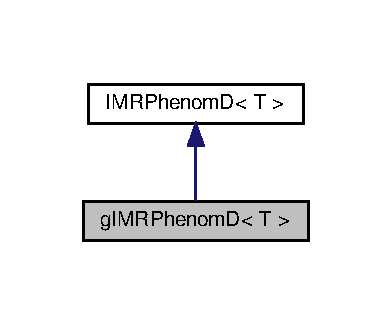
\includegraphics[width=188pt]{classgIMRPhenomD__inherit__graph}
\end{center}
\end{figure}


Collaboration diagram for g\+I\+M\+R\+PhenomD$<$ T $>$\+:\nopagebreak
\begin{figure}[H]
\begin{center}
\leavevmode
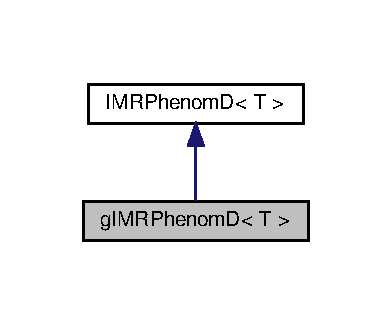
\includegraphics[width=188pt]{classgIMRPhenomD__coll__graph}
\end{center}
\end{figure}
\subsection*{Public Member Functions}
\begin{DoxyCompactItemize}
\item 
virtual T \hyperlink{classgIMRPhenomD_a7f4ebb4ae13d1038a437f86862f6dce1}{phase\+\_\+ins} (T f, \hyperlink{structsource__parameters}{source\+\_\+parameters}$<$ T $>$ $\ast$param, T $\ast$pn\+\_\+coeff, \hyperlink{structlambda__parameters}{lambda\+\_\+parameters}$<$ T $>$ $\ast$lambda, \hyperlink{structuseful__powers}{useful\+\_\+powers}$<$ T $>$ $\ast$pow)
\begin{DoxyCompactList}\small\item\em Calculates the inspiral phase for frequency f with precomputed powers of MF and PI for speed. \end{DoxyCompactList}\item 
virtual T \hyperlink{classgIMRPhenomD_a6099474bc9029be687ff6ede999ae5a7}{Dphase\+\_\+ins} (T f, \hyperlink{structsource__parameters}{source\+\_\+parameters}$<$ T $>$ $\ast$params, T $\ast$pn\+\_\+coeff, \hyperlink{structlambda__parameters}{lambda\+\_\+parameters}$<$ T $>$ $\ast$lambda)
\begin{DoxyCompactList}\small\item\em Calculates the derivative of the inspiral phase for frequency f. \end{DoxyCompactList}\item 
\mbox{\Hypertarget{classgIMRPhenomD_a21fa3ed99dc15dfe6e3d3174f14d115d}\label{classgIMRPhenomD_a21fa3ed99dc15dfe6e3d3174f14d115d}} 
virtual void \hyperlink{classgIMRPhenomD_a21fa3ed99dc15dfe6e3d3174f14d115d}{assign\+\_\+lambda\+\_\+param} (\hyperlink{structsource__parameters}{source\+\_\+parameters}$<$ T $>$ $\ast$source\+\_\+param, \hyperlink{structlambda__parameters}{lambda\+\_\+parameters}$<$ T $>$ $\ast$lambda)
\begin{DoxyCompactList}\small\item\em Wrapper for the Lambda parameter assignment that handles the looping. \end{DoxyCompactList}\item 
\mbox{\Hypertarget{classgIMRPhenomD_a6f9f182e4299198ad2ffc1eecdd41f10}\label{classgIMRPhenomD_a6f9f182e4299198ad2ffc1eecdd41f10}} 
virtual void \hyperlink{classgIMRPhenomD_a6f9f182e4299198ad2ffc1eecdd41f10}{assign\+\_\+static\+\_\+pn\+\_\+phase\+\_\+coeff} (\hyperlink{structsource__parameters}{source\+\_\+parameters}$<$ T $>$ $\ast$source\+\_\+param, T $\ast$coeff)
\begin{DoxyCompactList}\small\item\em Calculates the static PN coeffecients for the phase -\/ coeffecients 0,1,2,3,4,7. \end{DoxyCompactList}\end{DoxyCompactItemize}


\subsection{Member Function Documentation}
\mbox{\Hypertarget{classgIMRPhenomD_a6099474bc9029be687ff6ede999ae5a7}\label{classgIMRPhenomD_a6099474bc9029be687ff6ede999ae5a7}} 
\index{g\+I\+M\+R\+PhenomD@{g\+I\+M\+R\+PhenomD}!Dphase\+\_\+ins@{Dphase\+\_\+ins}}
\index{Dphase\+\_\+ins@{Dphase\+\_\+ins}!g\+I\+M\+R\+PhenomD@{g\+I\+M\+R\+PhenomD}}
\subsubsection{\texorpdfstring{Dphase\+\_\+ins()}{Dphase\_ins()}}
{\footnotesize\ttfamily template$<$class T $>$ \\
T \hyperlink{classgIMRPhenomD}{g\+I\+M\+R\+PhenomD}$<$ T $>$\+::Dphase\+\_\+ins (\begin{DoxyParamCaption}\item[{T}]{f,  }\item[{\hyperlink{structsource__parameters}{source\+\_\+parameters}$<$ T $>$ $\ast$}]{param,  }\item[{T $\ast$}]{pn\+\_\+coeff,  }\item[{\hyperlink{structlambda__parameters}{lambda\+\_\+parameters}$<$ T $>$ $\ast$}]{lambda }\end{DoxyParamCaption})\hspace{0.3cm}{\ttfamily [virtual]}}



Calculates the derivative of the inspiral phase for frequency f. 

For phase continuity and smoothness return a T 

Reimplemented from \hyperlink{classIMRPhenomD_ab840b052576cde8a9e802c5784d24092}{I\+M\+R\+Phenom\+D$<$ T $>$}.

\mbox{\Hypertarget{classgIMRPhenomD_a7f4ebb4ae13d1038a437f86862f6dce1}\label{classgIMRPhenomD_a7f4ebb4ae13d1038a437f86862f6dce1}} 
\index{g\+I\+M\+R\+PhenomD@{g\+I\+M\+R\+PhenomD}!phase\+\_\+ins@{phase\+\_\+ins}}
\index{phase\+\_\+ins@{phase\+\_\+ins}!g\+I\+M\+R\+PhenomD@{g\+I\+M\+R\+PhenomD}}
\subsubsection{\texorpdfstring{phase\+\_\+ins()}{phase\_ins()}}
{\footnotesize\ttfamily template$<$class T $>$ \\
T \hyperlink{classgIMRPhenomD}{g\+I\+M\+R\+PhenomD}$<$ T $>$\+::phase\+\_\+ins (\begin{DoxyParamCaption}\item[{T}]{f,  }\item[{\hyperlink{structsource__parameters}{source\+\_\+parameters}$<$ T $>$ $\ast$}]{param,  }\item[{T $\ast$}]{pn\+\_\+coeff,  }\item[{\hyperlink{structlambda__parameters}{lambda\+\_\+parameters}$<$ T $>$ $\ast$}]{lambda,  }\item[{\hyperlink{structuseful__powers}{useful\+\_\+powers}$<$ T $>$ $\ast$}]{pow }\end{DoxyParamCaption})\hspace{0.3cm}{\ttfamily [virtual]}}



Calculates the inspiral phase for frequency f with precomputed powers of MF and PI for speed. 

return a T

extra argument of precomputed powers of MF and pi, contained in the structure useful\+\_\+powers$<$\+T$>$ 

Reimplemented from \hyperlink{classIMRPhenomD_a7073ff2be22b0251ca419d0b69dd9990}{I\+M\+R\+Phenom\+D$<$ T $>$}.



The documentation for this class was generated from the following files\+:\begin{DoxyCompactItemize}
\item 
include/gwat/\hyperlink{gIMRPhenomD_8h}{g\+I\+M\+R\+Phenom\+D.\+h}\item 
src/\hyperlink{gIMRPhenomD_8cpp}{g\+I\+M\+R\+Phenom\+D.\+cpp}\end{DoxyCompactItemize}

\hypertarget{structGPUplan}{}\section{G\+P\+Uplan Struct Reference}
\label{structGPUplan}\index{G\+P\+Uplan@{G\+P\+Uplan}}
\subsection*{Public Attributes}
\begin{DoxyCompactItemize}
\item 
\mbox{\Hypertarget{structGPUplan_a7cc158ce31f5e5d3f06b5a71bd95a034}\label{structGPUplan_a7cc158ce31f5e5d3f06b5a71bd95a034}} 
int {\bfseries device\+\_\+id}
\item 
\mbox{\Hypertarget{structGPUplan_a0622e4ecd52a4f209ad12e6f5bf7e1c0}\label{structGPUplan_a0622e4ecd52a4f209ad12e6f5bf7e1c0}} 
double $\ast$ {\bfseries device\+\_\+data}
\item 
\mbox{\Hypertarget{structGPUplan_a00eb537157f28a6e1b0be9da32d3d7b9}\label{structGPUplan_a00eb537157f28a6e1b0be9da32d3d7b9}} 
double $\ast$ {\bfseries host\+\_\+data}
\item 
\mbox{\Hypertarget{structGPUplan_ac398a54fbf61c4bf193b970ff52867ea}\label{structGPUplan_ac398a54fbf61c4bf193b970ff52867ea}} 
int $\ast$ {\bfseries host\+\_\+lag}
\item 
\mbox{\Hypertarget{structGPUplan_a76a13cb6022abedf4397b15257277459}\label{structGPUplan_a76a13cb6022abedf4397b15257277459}} 
int $\ast$ {\bfseries device\+\_\+lag}
\item 
\mbox{\Hypertarget{structGPUplan_a994c924408e612fea29b4d97cab9b602}\label{structGPUplan_a994c924408e612fea29b4d97cab9b602}} 
int $\ast$ {\bfseries device\+\_\+lags}
\item 
\mbox{\Hypertarget{structGPUplan_af8314128bcabaeb61e435ff7149bf2e2}\label{structGPUplan_af8314128bcabaeb61e435ff7149bf2e2}} 
int $\ast$ {\bfseries initial\+\_\+lag}
\item 
\mbox{\Hypertarget{structGPUplan_a5c69f5f57401823335e968f6a2f2263c}\label{structGPUplan_a5c69f5f57401823335e968f6a2f2263c}} 
cuda\+Stream\+\_\+t {\bfseries stream}
\end{DoxyCompactItemize}


The documentation for this struct was generated from the following file\+:\begin{DoxyCompactItemize}
\item 
include/gwat/\hyperlink{autocorrelation__cuda_8hu}{autocorrelation\+\_\+cuda.\+hu}\end{DoxyCompactItemize}

\hypertarget{structgsl__snr__struct}{}\doxysection{gsl\+\_\+snr\+\_\+struct Struct Reference}
\label{structgsl__snr__struct}\index{gsl\_snr\_struct@{gsl\_snr\_struct}}


Collaboration diagram for gsl\+\_\+snr\+\_\+struct\+:
\nopagebreak
\begin{figure}[H]
\begin{center}
\leavevmode
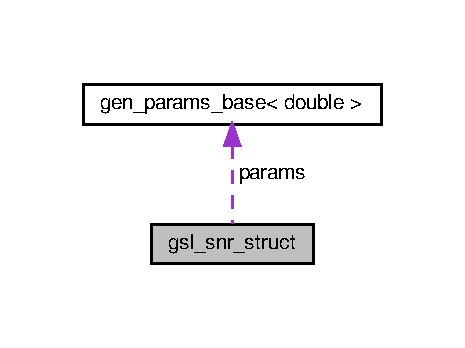
\includegraphics[width=223pt]{structgsl__snr__struct__coll__graph}
\end{center}
\end{figure}
\doxysubsection*{Public Attributes}
\begin{DoxyCompactItemize}
\item 
\mbox{\Hypertarget{structgsl__snr__struct_a0919a6d9e322d8c8192216608f39eaf1}\label{structgsl__snr__struct_a0919a6d9e322d8c8192216608f39eaf1}} 
\mbox{\hyperlink{classgen__params__base}{gen\+\_\+params\+\_\+base}}$<$ double $>$ $\ast$ {\bfseries params}
\item 
\mbox{\Hypertarget{structgsl__snr__struct_abb015712abe035f53feb741b1b41b48e}\label{structgsl__snr__struct_abb015712abe035f53feb741b1b41b48e}} 
std\+::string {\bfseries SN}
\item 
\mbox{\Hypertarget{structgsl__snr__struct_a0bb473cdde3594f18d424fcb09eabee2}\label{structgsl__snr__struct_a0bb473cdde3594f18d424fcb09eabee2}} 
std\+::string {\bfseries generation\+\_\+method}
\item 
\mbox{\Hypertarget{structgsl__snr__struct_ae828927fe7077e108a7f5e065efadae8}\label{structgsl__snr__struct_ae828927fe7077e108a7f5e065efadae8}} 
std\+::string {\bfseries detector}
\end{DoxyCompactItemize}


The documentation for this struct was generated from the following file\+:\begin{DoxyCompactItemize}
\item 
src/\mbox{\hyperlink{waveform__util_8cpp}{waveform\+\_\+util.\+cpp}}\end{DoxyCompactItemize}

\hypertarget{structgsl__subroutine}{}\doxysection{gsl\+\_\+subroutine Struct Reference}
\label{structgsl__subroutine}\index{gsl\_subroutine@{gsl\_subroutine}}


Collaboration diagram for gsl\+\_\+subroutine\+:
% FIG 0
\doxysubsection*{Public Attributes}
\begin{DoxyCompactItemize}
\item 
\mbox{\Hypertarget{structgsl__subroutine_a8d53607ed8fd837b5d584d7edbb39634}\label{structgsl__subroutine_a8d53607ed8fd837b5d584d7edbb39634}} 
string {\bfseries detector}
\item 
\mbox{\Hypertarget{structgsl__subroutine_a6366a126a6cf98adba59e0a803c152f4}\label{structgsl__subroutine_a6366a126a6cf98adba59e0a803c152f4}} 
string {\bfseries generation\+\_\+method}
\item 
\mbox{\Hypertarget{structgsl__subroutine_a4fdfc6d7026162cf7a8e8a1bf38ffe61}\label{structgsl__subroutine_a4fdfc6d7026162cf7a8e8a1bf38ffe61}} 
string {\bfseries sensitivity\+\_\+curve}
\item 
\mbox{\Hypertarget{structgsl__subroutine_aada6e2a926c6cc128411365dcd4586b9}\label{structgsl__subroutine_aada6e2a926c6cc128411365dcd4586b9}} 
\mbox{\hyperlink{classgen__params}{gen\+\_\+params}} $\ast$ {\bfseries gen\+\_\+params\+\_\+in}
\item 
\mbox{\Hypertarget{structgsl__subroutine_a0b8c2d6916f8e62f77d60f66dc10432d}\label{structgsl__subroutine_a0b8c2d6916f8e62f77d60f66dc10432d}} 
int {\bfseries dim}
\item 
\mbox{\Hypertarget{structgsl__subroutine_aaa9461cae596e1aa715db161e97725a5}\label{structgsl__subroutine_aaa9461cae596e1aa715db161e97725a5}} 
int {\bfseries id1}
\item 
\mbox{\Hypertarget{structgsl__subroutine_ac710432ac651e2044595ce56ffdc15d0}\label{structgsl__subroutine_ac710432ac651e2044595ce56ffdc15d0}} 
int {\bfseries id2}
\item 
\mbox{\Hypertarget{structgsl__subroutine_aa58cb5782b512416613b972625a9f61c}\label{structgsl__subroutine_aa58cb5782b512416613b972625a9f61c}} 
int $\ast$ {\bfseries waveform\+\_\+tapes}
\item 
\mbox{\Hypertarget{structgsl__subroutine_ae173f0d099a21774a228f9e6f1870d1f}\label{structgsl__subroutine_ae173f0d099a21774a228f9e6f1870d1f}} 
int $\ast$ {\bfseries time\+\_\+tapes}
\item 
\mbox{\Hypertarget{structgsl__subroutine_ae3f14cb143f4e7d1b6d0be279370ad26}\label{structgsl__subroutine_ae3f14cb143f4e7d1b6d0be279370ad26}} 
int $\ast$ {\bfseries phase\+\_\+tapes}
\item 
\mbox{\Hypertarget{structgsl__subroutine_a237d86fd52747febdafb2f88d5b6ebfd}\label{structgsl__subroutine_a237d86fd52747febdafb2f88d5b6ebfd}} 
double $\ast$ {\bfseries freq\+\_\+boundaries}
\item 
\mbox{\Hypertarget{structgsl__subroutine_a688679a9623a57de87458d7ea8426aba}\label{structgsl__subroutine_a688679a9623a57de87458d7ea8426aba}} 
double $\ast$ {\bfseries grad\+\_\+freqs}
\item 
\mbox{\Hypertarget{structgsl__subroutine_a5ec7158582cfcfe046b563a7b6c6e993}\label{structgsl__subroutine_a5ec7158582cfcfe046b563a7b6c6e993}} 
int {\bfseries boundary\+\_\+num}
\item 
\mbox{\Hypertarget{structgsl__subroutine_a0f17198c5a5e5848addabf9075c1dbac}\label{structgsl__subroutine_a0f17198c5a5e5848addabf9075c1dbac}} 
bool $\ast$ {\bfseries log\+\_\+factors}
\end{DoxyCompactItemize}


The documentation for this struct was generated from the following file\+:\begin{DoxyCompactItemize}
\item 
include/gwat/\mbox{\hyperlink{fisher_8h}{fisher.\+h}}\end{DoxyCompactItemize}

\hypertarget{classIMRPhenomD}{}\doxysection{I\+M\+R\+PhenomD$<$ T $>$ Class Template Reference}
\label{classIMRPhenomD}\index{IMRPhenomD$<$ T $>$@{IMRPhenomD$<$ T $>$}}


Inheritance diagram for I\+M\+R\+PhenomD$<$ T $>$\+:
% FIG 0
\doxysubsection*{Public Member Functions}
\begin{DoxyCompactItemize}
\item 
\mbox{\Hypertarget{classIMRPhenomD_aa11b2b18790e11237a1a4f1ad1036f6e}\label{classIMRPhenomD_aa11b2b18790e11237a1a4f1ad1036f6e}} 
virtual void {\bfseries fisher\+\_\+calculation\+\_\+sky\+\_\+averaged} (double $\ast$frequency, int length, \mbox{\hyperlink{classgen__params}{gen\+\_\+params}} $\ast$parameters, double $\ast$$\ast$amplitude\+\_\+deriv, double $\ast$$\ast$phase\+\_\+deriv, double $\ast$amplitude, int $\ast$amp\+\_\+tapes, int $\ast$phase\+\_\+tapes)
\item 
virtual void \mbox{\hyperlink{classIMRPhenomD_aa0e18ec42afcc215093b0c3a57580826}{change\+\_\+parameter\+\_\+basis}} (T $\ast$old\+\_\+param, T $\ast$new\+\_\+param, bool sky\+\_\+average)
\begin{DoxyCompactList}\small\item\em Convience method to change parameter basis between common Fisher parameters and the intrinsic parameters of \mbox{\hyperlink{classIMRPhenomD}{I\+M\+R\+PhenomD}}. \end{DoxyCompactList}\item 
virtual void \mbox{\hyperlink{classIMRPhenomD_a4142331cc7a6471d13274b1ac8727378}{construct\+\_\+amplitude\+\_\+derivative}} (double $\ast$frequencies, int length, int dimension, double $\ast$$\ast$amplitude\+\_\+derivative, \mbox{\hyperlink{structsource__parameters}{source\+\_\+parameters}}$<$ double $>$ $\ast$input\+\_\+params, int $\ast$tapes=N\+U\+LL)
\begin{DoxyCompactList}\small\item\em Construct the derivative of the amplitude for a given source evaluated by the given frequency. \end{DoxyCompactList}\item 
virtual void \mbox{\hyperlink{classIMRPhenomD_a26da276caf4c148016f558541d6914f6}{construct\+\_\+phase\+\_\+derivative}} (double $\ast$frequencies, int length, int dimension, double $\ast$$\ast$phase\+\_\+derivative, \mbox{\hyperlink{structsource__parameters}{source\+\_\+parameters}}$<$ double $>$ $\ast$input\+\_\+params, int $\ast$tapes=N\+U\+LL)
\begin{DoxyCompactList}\small\item\em Construct the derivative of the phase for a given source evaluated by the given frequency. \end{DoxyCompactList}\item 
virtual void \mbox{\hyperlink{classIMRPhenomD_a6fbe3c51ee3eb66d332dc87a9fdf5bd4}{amplitude\+\_\+tape}} (\mbox{\hyperlink{structsource__parameters}{source\+\_\+parameters}}$<$ double $>$ $\ast$input\+\_\+params, int $\ast$tape)
\begin{DoxyCompactList}\small\item\em Creates the tapes for derivatives of the amplitude. \end{DoxyCompactList}\item 
virtual void \mbox{\hyperlink{classIMRPhenomD_ae456c25f87c34487e6e05f9cf5d2d08c}{phase\+\_\+tape}} (\mbox{\hyperlink{structsource__parameters}{source\+\_\+parameters}}$<$ double $>$ $\ast$input\+\_\+params, int $\ast$tape)
\begin{DoxyCompactList}\small\item\em Creates the tapes for derivatives of phase. \end{DoxyCompactList}\item 
virtual int \mbox{\hyperlink{classIMRPhenomD_aa7192bf99437b49e0b4f27a342a79dae}{construct\+\_\+waveform}} (T $\ast$frequencies, int length, std\+::complex$<$ T $>$ $\ast$waveform, \mbox{\hyperlink{structsource__parameters}{source\+\_\+parameters}}$<$ T $>$ $\ast$params)
\begin{DoxyCompactList}\small\item\em Constructs the waveform as outlined by. \end{DoxyCompactList}\item 
virtual std\+::complex$<$ T $>$ \mbox{\hyperlink{classIMRPhenomD_a1c15236140d34ea2ae1d9a540af7bdab}{construct\+\_\+waveform}} (T frequency, \mbox{\hyperlink{structsource__parameters}{source\+\_\+parameters}}$<$ T $>$ $\ast$params)
\begin{DoxyCompactList}\small\item\em overloaded method to evaluate the waveform for one frequency instead of an array \end{DoxyCompactList}\item 
virtual int \mbox{\hyperlink{classIMRPhenomD_a95e7946061fa24fdb7a770dba02147be}{construct\+\_\+amplitude}} (T $\ast$frequencies, int length, T $\ast$amplitude, \mbox{\hyperlink{structsource__parameters}{source\+\_\+parameters}}$<$ T $>$ $\ast$params)
\begin{DoxyCompactList}\small\item\em Constructs the Amplitude as outlined by \mbox{\hyperlink{classIMRPhenomD}{I\+M\+R\+PhenomD}}. \end{DoxyCompactList}\item 
virtual int \mbox{\hyperlink{classIMRPhenomD_abcbaafd0dc4086d2abe1f5ce256908c2}{construct\+\_\+phase}} (T $\ast$frequencies, int length, T $\ast$phase, \mbox{\hyperlink{structsource__parameters}{source\+\_\+parameters}}$<$ T $>$ $\ast$params)
\begin{DoxyCompactList}\small\item\em Constructs the Phase as outlined by \mbox{\hyperlink{classIMRPhenomD}{I\+M\+R\+PhenomD}}. \end{DoxyCompactList}\item 
virtual T \mbox{\hyperlink{classIMRPhenomD_acf5645dc97b020ef468149883d1aca50}{build\+\_\+amp}} (T f, \mbox{\hyperlink{structlambda__parameters}{lambda\+\_\+parameters}}$<$ T $>$ $\ast$lambda, \mbox{\hyperlink{structsource__parameters}{source\+\_\+parameters}}$<$ T $>$ $\ast$params, \mbox{\hyperlink{structuseful__powers}{useful\+\_\+powers}}$<$ T $>$ $\ast$pows, T $\ast$amp\+\_\+coeff, T $\ast$deltas)
\begin{DoxyCompactList}\small\item\em constructs the \mbox{\hyperlink{classIMRPhenomD}{I\+M\+R\+PhenomD}} amplitude for frequency f \end{DoxyCompactList}\item 
virtual T \mbox{\hyperlink{classIMRPhenomD_a03ecb320683b9d2b6df6e943fc55cec7}{build\+\_\+phase}} (T f, \mbox{\hyperlink{structlambda__parameters}{lambda\+\_\+parameters}}$<$ T $>$ $\ast$lambda, \mbox{\hyperlink{structsource__parameters}{source\+\_\+parameters}}$<$ T $>$ $\ast$params, \mbox{\hyperlink{structuseful__powers}{useful\+\_\+powers}}$<$ T $>$ $\ast$pows, T $\ast$phase\+\_\+coeff)
\begin{DoxyCompactList}\small\item\em constructs the \mbox{\hyperlink{classIMRPhenomD}{I\+M\+R\+PhenomD}} phase for frequency f \end{DoxyCompactList}\item 
\mbox{\Hypertarget{classIMRPhenomD_a551588d127597037000512cfafa42673}\label{classIMRPhenomD_a551588d127597037000512cfafa42673}} 
virtual T \mbox{\hyperlink{classIMRPhenomD_a551588d127597037000512cfafa42673}{assign\+\_\+lambda\+\_\+param\+\_\+element}} (\mbox{\hyperlink{structsource__parameters}{source\+\_\+parameters}}$<$ T $>$ $\ast$source\+\_\+param, int i)
\begin{DoxyCompactList}\small\item\em Calculate the lambda parameters from Khan et al for element i. \end{DoxyCompactList}\item 
\mbox{\Hypertarget{classIMRPhenomD_ae14db26ad43c3b7b4a2a962a0af5ff24}\label{classIMRPhenomD_ae14db26ad43c3b7b4a2a962a0af5ff24}} 
virtual void \mbox{\hyperlink{classIMRPhenomD_ae14db26ad43c3b7b4a2a962a0af5ff24}{assign\+\_\+lambda\+\_\+param}} (\mbox{\hyperlink{structsource__parameters}{source\+\_\+parameters}}$<$ T $>$ $\ast$source\+\_\+param, \mbox{\hyperlink{structlambda__parameters}{lambda\+\_\+parameters}}$<$ T $>$ $\ast$lambda)
\begin{DoxyCompactList}\small\item\em Wrapper for the Lambda parameter assignment that handles the looping. \end{DoxyCompactList}\item 
virtual void \mbox{\hyperlink{classIMRPhenomD_ade98ea0729f58a3216ecec948dec9e4a}{precalc\+\_\+powers\+\_\+ins}} (T f, T M, \mbox{\hyperlink{structuseful__powers}{useful\+\_\+powers}}$<$ T $>$ $\ast$Mf\+\_\+pows)
\begin{DoxyCompactList}\small\item\em Pre-\/calculate powers of Mf, to speed up calculations for the inspiral waveform (both amplitude and phase. \end{DoxyCompactList}\item 
virtual void \mbox{\hyperlink{classIMRPhenomD_a1181334310432c4d69ede3a3b2b0fcdb}{precalc\+\_\+powers\+\_\+\+PI}} (\mbox{\hyperlink{structuseful__powers}{useful\+\_\+powers}}$<$ T $>$ $\ast$P\+I\+\_\+pows)
\begin{DoxyCompactList}\small\item\em Pre-\/calculate powers of pi, to speed up calculations for the inspiral phase. \end{DoxyCompactList}\item 
virtual void \mbox{\hyperlink{classIMRPhenomD_aa4647f539a66554bcc5066861328cf06}{precalc\+\_\+powers\+\_\+ins\+\_\+phase}} (T f, T M, \mbox{\hyperlink{structuseful__powers}{useful\+\_\+powers}}$<$ T $>$ $\ast$Mf\+\_\+pows)
\begin{DoxyCompactList}\small\item\em Pre-\/calculate powers of Mf, to speed up calculations for the inspiral phase. \end{DoxyCompactList}\item 
virtual void \mbox{\hyperlink{classIMRPhenomD_ac25dfdbacff0e696d752db44dd0a6c6b}{precalc\+\_\+powers\+\_\+ins\+\_\+amp}} (T f, T M, \mbox{\hyperlink{structuseful__powers}{useful\+\_\+powers}}$<$ T $>$ $\ast$Mf\+\_\+pows)
\begin{DoxyCompactList}\small\item\em Pre-\/calculate powers of Mf, to speed up calculations for the inspiral amplitude. \end{DoxyCompactList}\item 
\mbox{\Hypertarget{classIMRPhenomD_a48e215265b20ae41245713b3900306dc}\label{classIMRPhenomD_a48e215265b20ae41245713b3900306dc}} 
virtual void \mbox{\hyperlink{classIMRPhenomD_a48e215265b20ae41245713b3900306dc}{assign\+\_\+pn\+\_\+amplitude\+\_\+coeff}} (\mbox{\hyperlink{structsource__parameters}{source\+\_\+parameters}}$<$ T $>$ $\ast$source\+\_\+param, T $\ast$coeff)
\begin{DoxyCompactList}\small\item\em Calculates the static PN coeffecients for the amplitude. \end{DoxyCompactList}\item 
\mbox{\Hypertarget{classIMRPhenomD_aaee6c205b4dbd79e12177656ad84744c}\label{classIMRPhenomD_aaee6c205b4dbd79e12177656ad84744c}} 
virtual void \mbox{\hyperlink{classIMRPhenomD_aaee6c205b4dbd79e12177656ad84744c}{assign\+\_\+static\+\_\+pn\+\_\+phase\+\_\+coeff}} (\mbox{\hyperlink{structsource__parameters}{source\+\_\+parameters}}$<$ T $>$ $\ast$source\+\_\+param, T $\ast$coeff)
\begin{DoxyCompactList}\small\item\em Calculates the static PN coeffecients for the phase -\/ coeffecients 0,1,2,3,4,7. \end{DoxyCompactList}\item 
virtual void \mbox{\hyperlink{classIMRPhenomD_a0fce09494daa1fee6be8297b8f18dec4}{assign\+\_\+nonstatic\+\_\+pn\+\_\+phase\+\_\+coeff}} (\mbox{\hyperlink{structsource__parameters}{source\+\_\+parameters}}$<$ T $>$ $\ast$source\+\_\+param, T $\ast$coeff, T f)
\begin{DoxyCompactList}\small\item\em Calculates the dynamic PN phase coefficients 5,6. \end{DoxyCompactList}\item 
virtual void \mbox{\hyperlink{classIMRPhenomD_aa10c5932742768573488dbdfa8526bff}{assign\+\_\+nonstatic\+\_\+pn\+\_\+phase\+\_\+coeff\+\_\+deriv}} (\mbox{\hyperlink{structsource__parameters}{source\+\_\+parameters}}$<$ T $>$ $\ast$source\+\_\+param, T $\ast$Dcoeff, T f)
\begin{DoxyCompactList}\small\item\em Calculates the derivative of the dynamic PN phase coefficients 5,6. \end{DoxyCompactList}\item 
virtual void \mbox{\hyperlink{classIMRPhenomD_a0d33a9a937a36f395300bab4276102af}{post\+\_\+merger\+\_\+variables}} (\mbox{\hyperlink{structsource__parameters}{source\+\_\+parameters}}$<$ T $>$ $\ast$source\+\_\+param)
\begin{DoxyCompactList}\small\item\em Calculates the post-\/merger ringdown frequency and dampening frequency. \end{DoxyCompactList}\item 
\mbox{\Hypertarget{classIMRPhenomD_a3561d291b8e089224eb53d81b19b954f}\label{classIMRPhenomD_a3561d291b8e089224eb53d81b19b954f}} 
virtual void {\bfseries calc\+\_\+fring} (\mbox{\hyperlink{structsource__parameters}{source\+\_\+parameters}}$<$ T $>$ $\ast$source\+\_\+params)
\item 
\mbox{\Hypertarget{classIMRPhenomD_ad9457c9b6f014e1be5242c90811206c2}\label{classIMRPhenomD_ad9457c9b6f014e1be5242c90811206c2}} 
virtual void {\bfseries calc\+\_\+fdamp} (\mbox{\hyperlink{structsource__parameters}{source\+\_\+parameters}}$<$ T $>$ $\ast$source\+\_\+params)
\item 
\mbox{\Hypertarget{classIMRPhenomD_aca95715b46b019637d054e06a1ba1e8f}\label{classIMRPhenomD_aca95715b46b019637d054e06a1ba1e8f}} 
virtual T {\bfseries final\+\_\+spin} (\mbox{\hyperlink{structsource__parameters}{source\+\_\+parameters}}$<$ T $>$ $\ast$params)
\item 
virtual T \mbox{\hyperlink{classIMRPhenomD_a75e0b12192eec9c3b7278810236c20a3}{Final\+Spin0815\+\_\+s}} (T eta, T s)
\item 
virtual T \mbox{\hyperlink{classIMRPhenomD_af638fe3433f2367f9dfe6e2236a6b0ee}{Final\+Spin0815}} (T eta, T chi1, T chi2)
\item 
virtual T \mbox{\hyperlink{classIMRPhenomD_a1a9c4c6addd7c73be5bbcd835e92e815}{Erad\+Rational0815\+\_\+s}} (T eta, T s)
\item 
virtual T \mbox{\hyperlink{classIMRPhenomD_a08bc2e3d31a033e590e9e573d3cf914e}{Erad\+Rational0815}} (T eta, T chi1, T chi2)
\item 
virtual T \mbox{\hyperlink{classIMRPhenomD_a31c4222e9a39b6eadd42c4f6707d8245}{fpeak}} (\mbox{\hyperlink{structsource__parameters}{source\+\_\+parameters}}$<$ T $>$ $\ast$params, \mbox{\hyperlink{structlambda__parameters}{lambda\+\_\+parameters}}$<$ T $>$ $\ast$lambda)
\begin{DoxyCompactList}\small\item\em Solves for the peak frequency, where the waveform transitions from intermediate to merger-\/ringdown. \end{DoxyCompactList}\item 
virtual T \mbox{\hyperlink{classIMRPhenomD_aef404dca66beb6652663271fee31b8f8}{amp\+\_\+ins}} (T f, \mbox{\hyperlink{structsource__parameters}{source\+\_\+parameters}}$<$ T $>$ $\ast$param, T $\ast$pn\+\_\+coeff, \mbox{\hyperlink{structlambda__parameters}{lambda\+\_\+parameters}}$<$ T $>$ $\ast$lambda, \mbox{\hyperlink{structuseful__powers}{useful\+\_\+powers}}$<$ T $>$ $\ast$pow)
\begin{DoxyCompactList}\small\item\em Calculates the scaled inspiral amplitude A/\+A0 for frequency f with precomputed powers of MF and PI. \end{DoxyCompactList}\item 
virtual T \mbox{\hyperlink{classIMRPhenomD_a7661208087c747ebfb04b59e17d66d17}{Damp\+\_\+ins}} (T f, \mbox{\hyperlink{structsource__parameters}{source\+\_\+parameters}}$<$ T $>$ $\ast$param, T $\ast$pn\+\_\+coeff, \mbox{\hyperlink{structlambda__parameters}{lambda\+\_\+parameters}}$<$ T $>$ $\ast$lambda)
\begin{DoxyCompactList}\small\item\em Calculates the derivative wrt frequency for the scaled inspiral amplitude A/\+A0 for frequency f. \end{DoxyCompactList}\item 
virtual T \mbox{\hyperlink{classIMRPhenomD_a7073ff2be22b0251ca419d0b69dd9990}{phase\+\_\+ins}} (T f, \mbox{\hyperlink{structsource__parameters}{source\+\_\+parameters}}$<$ T $>$ $\ast$param, T $\ast$pn\+\_\+coeff, \mbox{\hyperlink{structlambda__parameters}{lambda\+\_\+parameters}}$<$ T $>$ $\ast$lambda, \mbox{\hyperlink{structuseful__powers}{useful\+\_\+powers}}$<$ T $>$ $\ast$pow)
\begin{DoxyCompactList}\small\item\em Calculates the inspiral phase for frequency f with precomputed powers of MF and PI for speed. \end{DoxyCompactList}\item 
virtual T \mbox{\hyperlink{classIMRPhenomD_ab840b052576cde8a9e802c5784d24092}{Dphase\+\_\+ins}} (T f, \mbox{\hyperlink{structsource__parameters}{source\+\_\+parameters}}$<$ T $>$ $\ast$param, T $\ast$pn\+\_\+coeff, \mbox{\hyperlink{structlambda__parameters}{lambda\+\_\+parameters}}$<$ T $>$ $\ast$lambda)
\begin{DoxyCompactList}\small\item\em Calculates the derivative of the inspiral phase for frequency f. \end{DoxyCompactList}\item 
virtual T \mbox{\hyperlink{classIMRPhenomD_ad39d45f582ed9089b3783f7340eac615}{amp\+\_\+mr}} (T f, \mbox{\hyperlink{structsource__parameters}{source\+\_\+parameters}}$<$ T $>$ $\ast$param, \mbox{\hyperlink{structlambda__parameters}{lambda\+\_\+parameters}}$<$ T $>$ $\ast$lambda)
\begin{DoxyCompactList}\small\item\em Calculates the scaled merger-\/ringdown amplitude A/\+A0 for frequency f. \end{DoxyCompactList}\item 
virtual T \mbox{\hyperlink{classIMRPhenomD_a2c9c226afc991458872e36bba204f395}{phase\+\_\+mr}} (T f, \mbox{\hyperlink{structsource__parameters}{source\+\_\+parameters}}$<$ T $>$ $\ast$param, \mbox{\hyperlink{structlambda__parameters}{lambda\+\_\+parameters}}$<$ T $>$ $\ast$lambda)
\begin{DoxyCompactList}\small\item\em Calculates the merger-\/ringdown phase for frequency f. \end{DoxyCompactList}\item 
virtual T \mbox{\hyperlink{classIMRPhenomD_a59796cb7f1ac68684562508a5a83d505}{Damp\+\_\+mr}} (T f, \mbox{\hyperlink{structsource__parameters}{source\+\_\+parameters}}$<$ T $>$ $\ast$param, \mbox{\hyperlink{structlambda__parameters}{lambda\+\_\+parameters}}$<$ T $>$ $\ast$lambda)
\begin{DoxyCompactList}\small\item\em Calculates the derivative wrt frequency for the scaled merger-\/ringdown amplitude A/\+A0 for frequency f. \end{DoxyCompactList}\item 
virtual T \mbox{\hyperlink{classIMRPhenomD_ab4a74828eacee645bac43b0af2c510e1}{Dphase\+\_\+mr}} (T f, \mbox{\hyperlink{structsource__parameters}{source\+\_\+parameters}}$<$ T $>$ $\ast$param, \mbox{\hyperlink{structlambda__parameters}{lambda\+\_\+parameters}}$<$ T $>$ $\ast$lambda)
\begin{DoxyCompactList}\small\item\em Calculates the derivative of the merger-\/ringdown phase for frequency f. \end{DoxyCompactList}\item 
virtual T \mbox{\hyperlink{classIMRPhenomD_a7deef6d5f185eeff45bb7a3357fbd052}{amp\+\_\+int}} (T f, \mbox{\hyperlink{structsource__parameters}{source\+\_\+parameters}}$<$ T $>$ $\ast$param, \mbox{\hyperlink{structlambda__parameters}{lambda\+\_\+parameters}}$<$ T $>$ $\ast$lambda, T $\ast$deltas)
\begin{DoxyCompactList}\small\item\em Calculates the scaled intermediate range amplitude A/\+A0 for frequency f. \end{DoxyCompactList}\item 
virtual T \mbox{\hyperlink{classIMRPhenomD_ad6a8bb9539e7494cad8a91aaa950cf50}{phase\+\_\+int}} (T f, \mbox{\hyperlink{structsource__parameters}{source\+\_\+parameters}}$<$ T $>$ $\ast$param, \mbox{\hyperlink{structlambda__parameters}{lambda\+\_\+parameters}}$<$ T $>$ $\ast$lambda)
\begin{DoxyCompactList}\small\item\em Calculates the intermediate phase for frequency f. \end{DoxyCompactList}\item 
virtual T \mbox{\hyperlink{classIMRPhenomD_a8d395e33bd420cdc996a6487302af36a}{Dphase\+\_\+int}} (T f, \mbox{\hyperlink{structsource__parameters}{source\+\_\+parameters}}$<$ T $>$ $\ast$param, \mbox{\hyperlink{structlambda__parameters}{lambda\+\_\+parameters}}$<$ T $>$ $\ast$lambda)
\begin{DoxyCompactList}\small\item\em Calculates the derivative of the intermediate phase for frequency f. \end{DoxyCompactList}\item 
virtual void \mbox{\hyperlink{classIMRPhenomD_a6847c2c48302ff863b9a93354e71afcc}{phase\+\_\+connection\+\_\+coefficients}} (\mbox{\hyperlink{structsource__parameters}{source\+\_\+parameters}}$<$ T $>$ $\ast$param, \mbox{\hyperlink{structlambda__parameters}{lambda\+\_\+parameters}}$<$ T $>$ $\ast$lambda, T $\ast$pn\+\_\+coeffs)
\begin{DoxyCompactList}\small\item\em Calculates the phase connection coefficients alpha\{0,1\} and beta\{0,1\}. \end{DoxyCompactList}\item 
\mbox{\Hypertarget{classIMRPhenomD_a343638375f42abb5097f26ef3fe183ad}\label{classIMRPhenomD_a343638375f42abb5097f26ef3fe183ad}} 
virtual T {\bfseries calculate\+\_\+beta1} (\mbox{\hyperlink{structsource__parameters}{source\+\_\+parameters}}$<$ T $>$ $\ast$param, \mbox{\hyperlink{structlambda__parameters}{lambda\+\_\+parameters}}$<$ T $>$ $\ast$lambda, T $\ast$pn\+\_\+coeffs)
\item 
\mbox{\Hypertarget{classIMRPhenomD_ac3c4886ba5fafea197b2c8be90a04e63}\label{classIMRPhenomD_ac3c4886ba5fafea197b2c8be90a04e63}} 
virtual T {\bfseries calculate\+\_\+beta0} (\mbox{\hyperlink{structsource__parameters}{source\+\_\+parameters}}$<$ T $>$ $\ast$param, \mbox{\hyperlink{structlambda__parameters}{lambda\+\_\+parameters}}$<$ T $>$ $\ast$lambda, T $\ast$pn\+\_\+coeffs)
\item 
\mbox{\Hypertarget{classIMRPhenomD_a5bcd7d9b753b0e6acc9c74618ae484ad}\label{classIMRPhenomD_a5bcd7d9b753b0e6acc9c74618ae484ad}} 
virtual T {\bfseries calculate\+\_\+alpha1} (\mbox{\hyperlink{structsource__parameters}{source\+\_\+parameters}}$<$ T $>$ $\ast$param, \mbox{\hyperlink{structlambda__parameters}{lambda\+\_\+parameters}}$<$ T $>$ $\ast$lambda)
\item 
\mbox{\Hypertarget{classIMRPhenomD_aa8686f48edea51188f5a9168009ad677}\label{classIMRPhenomD_aa8686f48edea51188f5a9168009ad677}} 
virtual T {\bfseries calculate\+\_\+alpha0} (\mbox{\hyperlink{structsource__parameters}{source\+\_\+parameters}}$<$ T $>$ $\ast$param, \mbox{\hyperlink{structlambda__parameters}{lambda\+\_\+parameters}}$<$ T $>$ $\ast$lambda)
\item 
\mbox{\Hypertarget{classIMRPhenomD_aa945ea05c7846632798d29c88ae85ac9}\label{classIMRPhenomD_aa945ea05c7846632798d29c88ae85ac9}} 
virtual void \mbox{\hyperlink{classIMRPhenomD_aa945ea05c7846632798d29c88ae85ac9}{amp\+\_\+connection\+\_\+coeffs}} (\mbox{\hyperlink{structsource__parameters}{source\+\_\+parameters}}$<$ T $>$ $\ast$param, \mbox{\hyperlink{structlambda__parameters}{lambda\+\_\+parameters}}$<$ T $>$ $\ast$lambda, T $\ast$pn\+\_\+coeffs, T $\ast$coeffs)
\begin{DoxyCompactList}\small\item\em Solves for the connection coefficients to ensure the transition from inspiral to merger ringdown is continuous and smooth. \end{DoxyCompactList}\item 
virtual T \mbox{\hyperlink{classIMRPhenomD_abd81c0aa321c96077823483c91ae01d4}{calculate\+\_\+delta\+\_\+parameter\+\_\+0}} (T f1, T f2, T f3, T v1, T v2, T v3, T dd1, T dd3, T M)
\begin{DoxyCompactList}\small\item\em Calculates the delta\+\_\+0 component. \end{DoxyCompactList}\item 
virtual T \mbox{\hyperlink{classIMRPhenomD_a6fd680e8cace47a635e7c3956dfb4b32}{calculate\+\_\+delta\+\_\+parameter\+\_\+1}} (T f1, T f2, T f3, T v1, T v2, T v3, T dd1, T dd3, T M)
\begin{DoxyCompactList}\small\item\em Calculates the delta\+\_\+1 component. \end{DoxyCompactList}\item 
virtual T \mbox{\hyperlink{classIMRPhenomD_acc1918553367dbe59ffb4959b0a0f5b2}{calculate\+\_\+delta\+\_\+parameter\+\_\+2}} (T f1, T f2, T f3, T v1, T v2, T v3, T dd1, T dd3, T M)
\begin{DoxyCompactList}\small\item\em Calculates the delta\+\_\+2 component. \end{DoxyCompactList}\item 
virtual T \mbox{\hyperlink{classIMRPhenomD_a4201abf06608c7a11adfee232f7eb581}{calculate\+\_\+delta\+\_\+parameter\+\_\+3}} (T f1, T f2, T f3, T v1, T v2, T v3, T dd1, T dd3, T M)
\begin{DoxyCompactList}\small\item\em Calculates the delta\+\_\+3 component. \end{DoxyCompactList}\item 
virtual T \mbox{\hyperlink{classIMRPhenomD_a22f9b0bc83c4ed555a46b03260c0d91d}{calculate\+\_\+delta\+\_\+parameter\+\_\+4}} (T f1, T f2, T f3, T v1, T v2, T v3, T dd1, T dd3, T M)
\begin{DoxyCompactList}\small\item\em Calculates the delta\+\_\+4 component. \end{DoxyCompactList}\item 
\mbox{\Hypertarget{classIMRPhenomD_a8fd3848d62fd8202024d66989118ced6}\label{classIMRPhenomD_a8fd3848d62fd8202024d66989118ced6}} 
{\footnotesize template$<$$>$ }\\void {\bfseries calc\+\_\+fring} (\mbox{\hyperlink{structsource__parameters}{source\+\_\+parameters}}$<$ double $>$ $\ast$source\+\_\+param)
\item 
\mbox{\Hypertarget{classIMRPhenomD_a0ff9e9a2cbccaa7c8fc7b91ce9f4ce98}\label{classIMRPhenomD_a0ff9e9a2cbccaa7c8fc7b91ce9f4ce98}} 
{\footnotesize template$<$$>$ }\\void {\bfseries calc\+\_\+fdamp} (\mbox{\hyperlink{structsource__parameters}{source\+\_\+parameters}}$<$ double $>$ $\ast$source\+\_\+param)
\item 
\mbox{\Hypertarget{classIMRPhenomD_a525e0691c320caf54ed7602407ac47ca}\label{classIMRPhenomD_a525e0691c320caf54ed7602407ac47ca}} 
{\footnotesize template$<$$>$ }\\void {\bfseries calc\+\_\+fring} (\mbox{\hyperlink{structsource__parameters}{source\+\_\+parameters}}$<$ adouble $>$ $\ast$source\+\_\+param)
\item 
\mbox{\Hypertarget{classIMRPhenomD_aedf9810e29b33dc7ab01b2fbe0b85eac}\label{classIMRPhenomD_aedf9810e29b33dc7ab01b2fbe0b85eac}} 
{\footnotesize template$<$$>$ }\\void {\bfseries calc\+\_\+fdamp} (\mbox{\hyperlink{structsource__parameters}{source\+\_\+parameters}}$<$ adouble $>$ $\ast$source\+\_\+param)
\end{DoxyCompactItemize}


\doxysubsection{Member Function Documentation}
\mbox{\Hypertarget{classIMRPhenomD_aef404dca66beb6652663271fee31b8f8}\label{classIMRPhenomD_aef404dca66beb6652663271fee31b8f8}} 
\index{IMRPhenomD$<$ T $>$@{IMRPhenomD$<$ T $>$}!amp\_ins@{amp\_ins}}
\index{amp\_ins@{amp\_ins}!IMRPhenomD$<$ T $>$@{IMRPhenomD$<$ T $>$}}
\doxysubsubsection{\texorpdfstring{amp\_ins()}{amp\_ins()}}
{\footnotesize\ttfamily template$<$class T $>$ \\
T \mbox{\hyperlink{classIMRPhenomD}{I\+M\+R\+PhenomD}}$<$ T $>$\+::amp\+\_\+ins (\begin{DoxyParamCaption}\item[{T}]{f,  }\item[{\mbox{\hyperlink{structsource__parameters}{source\+\_\+parameters}}$<$ T $>$ $\ast$}]{param,  }\item[{T $\ast$}]{pn\+\_\+coeff,  }\item[{\mbox{\hyperlink{structlambda__parameters}{lambda\+\_\+parameters}}$<$ T $>$ $\ast$}]{lambda,  }\item[{\mbox{\hyperlink{structuseful__powers}{useful\+\_\+powers}}$<$ T $>$ $\ast$}]{pow }\end{DoxyParamCaption})\hspace{0.3cm}{\ttfamily [virtual]}}



Calculates the scaled inspiral amplitude A/\+A0 for frequency f with precomputed powers of MF and PI. 

return a T

additional argument contains useful powers of MF and PI in structure userful\+\_\+powers \mbox{\Hypertarget{classIMRPhenomD_a7deef6d5f185eeff45bb7a3357fbd052}\label{classIMRPhenomD_a7deef6d5f185eeff45bb7a3357fbd052}} 
\index{IMRPhenomD$<$ T $>$@{IMRPhenomD$<$ T $>$}!amp\_int@{amp\_int}}
\index{amp\_int@{amp\_int}!IMRPhenomD$<$ T $>$@{IMRPhenomD$<$ T $>$}}
\doxysubsubsection{\texorpdfstring{amp\_int()}{amp\_int()}}
{\footnotesize\ttfamily template$<$class T $>$ \\
T \mbox{\hyperlink{classIMRPhenomD}{I\+M\+R\+PhenomD}}$<$ T $>$\+::amp\+\_\+int (\begin{DoxyParamCaption}\item[{T}]{f,  }\item[{\mbox{\hyperlink{structsource__parameters}{source\+\_\+parameters}}$<$ T $>$ $\ast$}]{param,  }\item[{\mbox{\hyperlink{structlambda__parameters}{lambda\+\_\+parameters}}$<$ T $>$ $\ast$}]{lambda,  }\item[{T $\ast$}]{deltas }\end{DoxyParamCaption})\hspace{0.3cm}{\ttfamily [virtual]}}



Calculates the scaled intermediate range amplitude A/\+A0 for frequency f. 

return a T \mbox{\Hypertarget{classIMRPhenomD_ad39d45f582ed9089b3783f7340eac615}\label{classIMRPhenomD_ad39d45f582ed9089b3783f7340eac615}} 
\index{IMRPhenomD$<$ T $>$@{IMRPhenomD$<$ T $>$}!amp\_mr@{amp\_mr}}
\index{amp\_mr@{amp\_mr}!IMRPhenomD$<$ T $>$@{IMRPhenomD$<$ T $>$}}
\doxysubsubsection{\texorpdfstring{amp\_mr()}{amp\_mr()}}
{\footnotesize\ttfamily template$<$class T $>$ \\
T \mbox{\hyperlink{classIMRPhenomD}{I\+M\+R\+PhenomD}}$<$ T $>$\+::amp\+\_\+mr (\begin{DoxyParamCaption}\item[{T}]{f,  }\item[{\mbox{\hyperlink{structsource__parameters}{source\+\_\+parameters}}$<$ T $>$ $\ast$}]{param,  }\item[{\mbox{\hyperlink{structlambda__parameters}{lambda\+\_\+parameters}}$<$ T $>$ $\ast$}]{lambda }\end{DoxyParamCaption})\hspace{0.3cm}{\ttfamily [virtual]}}



Calculates the scaled merger-\/ringdown amplitude A/\+A0 for frequency f. 

return a T \mbox{\Hypertarget{classIMRPhenomD_a6fbe3c51ee3eb66d332dc87a9fdf5bd4}\label{classIMRPhenomD_a6fbe3c51ee3eb66d332dc87a9fdf5bd4}} 
\index{IMRPhenomD$<$ T $>$@{IMRPhenomD$<$ T $>$}!amplitude\_tape@{amplitude\_tape}}
\index{amplitude\_tape@{amplitude\_tape}!IMRPhenomD$<$ T $>$@{IMRPhenomD$<$ T $>$}}
\doxysubsubsection{\texorpdfstring{amplitude\_tape()}{amplitude\_tape()}}
{\footnotesize\ttfamily template$<$class T $>$ \\
void \mbox{\hyperlink{classIMRPhenomD}{I\+M\+R\+PhenomD}}$<$ T $>$\+::amplitude\+\_\+tape (\begin{DoxyParamCaption}\item[{\mbox{\hyperlink{structsource__parameters}{source\+\_\+parameters}}$<$ double $>$ $\ast$}]{input\+\_\+params,  }\item[{int $\ast$}]{tape }\end{DoxyParamCaption})\hspace{0.3cm}{\ttfamily [virtual]}}



Creates the tapes for derivatives of the amplitude. 

For efficiency in long runs of large sets of fishers, the tapes can be precomputed and reused 
\begin{DoxyParams}{Parameters}
{\em input\+\_\+params} & source parameters structure of the desired source \\
\hline
{\em tape} & tape ids \\
\hline
\end{DoxyParams}


Reimplemented in \mbox{\hyperlink{classppE__IMRPhenomD__IMR_a3119a07c11ed53ae94823b11c5234c4f}{pp\+E\+\_\+\+I\+M\+R\+Phenom\+D\+\_\+\+I\+M\+R$<$ T $>$}}, and \mbox{\hyperlink{classppE__IMRPhenomD__Inspiral_a87474cac9d6086d5625f79e28970b5ed}{pp\+E\+\_\+\+I\+M\+R\+Phenom\+D\+\_\+\+Inspiral$<$ T $>$}}.

\mbox{\Hypertarget{classIMRPhenomD_a0fce09494daa1fee6be8297b8f18dec4}\label{classIMRPhenomD_a0fce09494daa1fee6be8297b8f18dec4}} 
\index{IMRPhenomD$<$ T $>$@{IMRPhenomD$<$ T $>$}!assign\_nonstatic\_pn\_phase\_coeff@{assign\_nonstatic\_pn\_phase\_coeff}}
\index{assign\_nonstatic\_pn\_phase\_coeff@{assign\_nonstatic\_pn\_phase\_coeff}!IMRPhenomD$<$ T $>$@{IMRPhenomD$<$ T $>$}}
\doxysubsubsection{\texorpdfstring{assign\_nonstatic\_pn\_phase\_coeff()}{assign\_nonstatic\_pn\_phase\_coeff()}}
{\footnotesize\ttfamily template$<$class T $>$ \\
void \mbox{\hyperlink{classIMRPhenomD}{I\+M\+R\+PhenomD}}$<$ T $>$\+::assign\+\_\+nonstatic\+\_\+pn\+\_\+phase\+\_\+coeff (\begin{DoxyParamCaption}\item[{\mbox{\hyperlink{structsource__parameters}{source\+\_\+parameters}}$<$ T $>$ $\ast$}]{source\+\_\+param,  }\item[{T $\ast$}]{coeff,  }\item[{T}]{f }\end{DoxyParamCaption})\hspace{0.3cm}{\ttfamily [virtual]}}



Calculates the dynamic PN phase coefficients 5,6. 

f is in Hz \mbox{\Hypertarget{classIMRPhenomD_aa10c5932742768573488dbdfa8526bff}\label{classIMRPhenomD_aa10c5932742768573488dbdfa8526bff}} 
\index{IMRPhenomD$<$ T $>$@{IMRPhenomD$<$ T $>$}!assign\_nonstatic\_pn\_phase\_coeff\_deriv@{assign\_nonstatic\_pn\_phase\_coeff\_deriv}}
\index{assign\_nonstatic\_pn\_phase\_coeff\_deriv@{assign\_nonstatic\_pn\_phase\_coeff\_deriv}!IMRPhenomD$<$ T $>$@{IMRPhenomD$<$ T $>$}}
\doxysubsubsection{\texorpdfstring{assign\_nonstatic\_pn\_phase\_coeff\_deriv()}{assign\_nonstatic\_pn\_phase\_coeff\_deriv()}}
{\footnotesize\ttfamily template$<$class T $>$ \\
void \mbox{\hyperlink{classIMRPhenomD}{I\+M\+R\+PhenomD}}$<$ T $>$\+::assign\+\_\+nonstatic\+\_\+pn\+\_\+phase\+\_\+coeff\+\_\+deriv (\begin{DoxyParamCaption}\item[{\mbox{\hyperlink{structsource__parameters}{source\+\_\+parameters}}$<$ T $>$ $\ast$}]{source\+\_\+param,  }\item[{T $\ast$}]{Dcoeff,  }\item[{T}]{f }\end{DoxyParamCaption})\hspace{0.3cm}{\ttfamily [virtual]}}



Calculates the derivative of the dynamic PN phase coefficients 5,6. 

f is in Hz \mbox{\Hypertarget{classIMRPhenomD_acf5645dc97b020ef468149883d1aca50}\label{classIMRPhenomD_acf5645dc97b020ef468149883d1aca50}} 
\index{IMRPhenomD$<$ T $>$@{IMRPhenomD$<$ T $>$}!build\_amp@{build\_amp}}
\index{build\_amp@{build\_amp}!IMRPhenomD$<$ T $>$@{IMRPhenomD$<$ T $>$}}
\doxysubsubsection{\texorpdfstring{build\_amp()}{build\_amp()}}
{\footnotesize\ttfamily template$<$class T $>$ \\
T \mbox{\hyperlink{classIMRPhenomD}{I\+M\+R\+PhenomD}}$<$ T $>$\+::build\+\_\+amp (\begin{DoxyParamCaption}\item[{T}]{f,  }\item[{\mbox{\hyperlink{structlambda__parameters}{lambda\+\_\+parameters}}$<$ T $>$ $\ast$}]{lambda,  }\item[{\mbox{\hyperlink{structsource__parameters}{source\+\_\+parameters}}$<$ T $>$ $\ast$}]{params,  }\item[{\mbox{\hyperlink{structuseful__powers}{useful\+\_\+powers}}$<$ T $>$ $\ast$}]{pows,  }\item[{T $\ast$}]{amp\+\_\+coeff,  }\item[{T $\ast$}]{deltas }\end{DoxyParamCaption})\hspace{0.3cm}{\ttfamily [virtual]}}



constructs the \mbox{\hyperlink{classIMRPhenomD}{I\+M\+R\+PhenomD}} amplitude for frequency f 

arguments\+: numerical parameters from Khan et al \mbox{\hyperlink{structlambda__parameters}{lambda\+\_\+parameters}} structure, \mbox{\hyperlink{structsource__parameters}{source\+\_\+parameters}} structure, useful\+\_\+powers$<$\+T$>$ structure, PN parameters for the inspiral portions of the waveform, and the delta parameters for the intermediate region, numerically solved for using the amp\+\_\+connection\+\_\+coeffs function \mbox{\Hypertarget{classIMRPhenomD_a03ecb320683b9d2b6df6e943fc55cec7}\label{classIMRPhenomD_a03ecb320683b9d2b6df6e943fc55cec7}} 
\index{IMRPhenomD$<$ T $>$@{IMRPhenomD$<$ T $>$}!build\_phase@{build\_phase}}
\index{build\_phase@{build\_phase}!IMRPhenomD$<$ T $>$@{IMRPhenomD$<$ T $>$}}
\doxysubsubsection{\texorpdfstring{build\_phase()}{build\_phase()}}
{\footnotesize\ttfamily template$<$class T $>$ \\
T \mbox{\hyperlink{classIMRPhenomD}{I\+M\+R\+PhenomD}}$<$ T $>$\+::build\+\_\+phase (\begin{DoxyParamCaption}\item[{T}]{f,  }\item[{\mbox{\hyperlink{structlambda__parameters}{lambda\+\_\+parameters}}$<$ T $>$ $\ast$}]{lambda,  }\item[{\mbox{\hyperlink{structsource__parameters}{source\+\_\+parameters}}$<$ T $>$ $\ast$}]{params,  }\item[{\mbox{\hyperlink{structuseful__powers}{useful\+\_\+powers}}$<$ T $>$ $\ast$}]{pows,  }\item[{T $\ast$}]{phase\+\_\+coeff }\end{DoxyParamCaption})\hspace{0.3cm}{\ttfamily [virtual]}}



constructs the \mbox{\hyperlink{classIMRPhenomD}{I\+M\+R\+PhenomD}} phase for frequency f 

arguments\+: numerical parameters from Khan et al \mbox{\hyperlink{structlambda__parameters}{lambda\+\_\+parameters}} structure, \mbox{\hyperlink{structsource__parameters}{source\+\_\+parameters}} structure, \mbox{\hyperlink{structuseful__powers}{useful\+\_\+powers}} structure, PN parameters for the inspiral portions of the waveform \mbox{\Hypertarget{classIMRPhenomD_abd81c0aa321c96077823483c91ae01d4}\label{classIMRPhenomD_abd81c0aa321c96077823483c91ae01d4}} 
\index{IMRPhenomD$<$ T $>$@{IMRPhenomD$<$ T $>$}!calculate\_delta\_parameter\_0@{calculate\_delta\_parameter\_0}}
\index{calculate\_delta\_parameter\_0@{calculate\_delta\_parameter\_0}!IMRPhenomD$<$ T $>$@{IMRPhenomD$<$ T $>$}}
\doxysubsubsection{\texorpdfstring{calculate\_delta\_parameter\_0()}{calculate\_delta\_parameter\_0()}}
{\footnotesize\ttfamily template$<$class T $>$ \\
T \mbox{\hyperlink{classIMRPhenomD}{I\+M\+R\+PhenomD}}$<$ T $>$\+::calculate\+\_\+delta\+\_\+parameter\+\_\+0 (\begin{DoxyParamCaption}\item[{T}]{f1,  }\item[{T}]{f2,  }\item[{T}]{f3,  }\item[{T}]{v1,  }\item[{T}]{v2,  }\item[{T}]{v3,  }\item[{T}]{dd1,  }\item[{T}]{dd3,  }\item[{T}]{M }\end{DoxyParamCaption})\hspace{0.3cm}{\ttfamily [virtual]}}



Calculates the delta\+\_\+0 component. 

Solved in Mathematica and imported to C \mbox{\Hypertarget{classIMRPhenomD_a6fd680e8cace47a635e7c3956dfb4b32}\label{classIMRPhenomD_a6fd680e8cace47a635e7c3956dfb4b32}} 
\index{IMRPhenomD$<$ T $>$@{IMRPhenomD$<$ T $>$}!calculate\_delta\_parameter\_1@{calculate\_delta\_parameter\_1}}
\index{calculate\_delta\_parameter\_1@{calculate\_delta\_parameter\_1}!IMRPhenomD$<$ T $>$@{IMRPhenomD$<$ T $>$}}
\doxysubsubsection{\texorpdfstring{calculate\_delta\_parameter\_1()}{calculate\_delta\_parameter\_1()}}
{\footnotesize\ttfamily template$<$class T $>$ \\
T \mbox{\hyperlink{classIMRPhenomD}{I\+M\+R\+PhenomD}}$<$ T $>$\+::calculate\+\_\+delta\+\_\+parameter\+\_\+1 (\begin{DoxyParamCaption}\item[{T}]{f1,  }\item[{T}]{f2,  }\item[{T}]{f3,  }\item[{T}]{v1,  }\item[{T}]{v2,  }\item[{T}]{v3,  }\item[{T}]{dd1,  }\item[{T}]{dd3,  }\item[{T}]{M }\end{DoxyParamCaption})\hspace{0.3cm}{\ttfamily [virtual]}}



Calculates the delta\+\_\+1 component. 

Solved in Mathematica and imported to C \mbox{\Hypertarget{classIMRPhenomD_acc1918553367dbe59ffb4959b0a0f5b2}\label{classIMRPhenomD_acc1918553367dbe59ffb4959b0a0f5b2}} 
\index{IMRPhenomD$<$ T $>$@{IMRPhenomD$<$ T $>$}!calculate\_delta\_parameter\_2@{calculate\_delta\_parameter\_2}}
\index{calculate\_delta\_parameter\_2@{calculate\_delta\_parameter\_2}!IMRPhenomD$<$ T $>$@{IMRPhenomD$<$ T $>$}}
\doxysubsubsection{\texorpdfstring{calculate\_delta\_parameter\_2()}{calculate\_delta\_parameter\_2()}}
{\footnotesize\ttfamily template$<$class T $>$ \\
T \mbox{\hyperlink{classIMRPhenomD}{I\+M\+R\+PhenomD}}$<$ T $>$\+::calculate\+\_\+delta\+\_\+parameter\+\_\+2 (\begin{DoxyParamCaption}\item[{T}]{f1,  }\item[{T}]{f2,  }\item[{T}]{f3,  }\item[{T}]{v1,  }\item[{T}]{v2,  }\item[{T}]{v3,  }\item[{T}]{dd1,  }\item[{T}]{dd3,  }\item[{T}]{M }\end{DoxyParamCaption})\hspace{0.3cm}{\ttfamily [virtual]}}



Calculates the delta\+\_\+2 component. 

Solved in Mathematica and imported to C \mbox{\Hypertarget{classIMRPhenomD_a4201abf06608c7a11adfee232f7eb581}\label{classIMRPhenomD_a4201abf06608c7a11adfee232f7eb581}} 
\index{IMRPhenomD$<$ T $>$@{IMRPhenomD$<$ T $>$}!calculate\_delta\_parameter\_3@{calculate\_delta\_parameter\_3}}
\index{calculate\_delta\_parameter\_3@{calculate\_delta\_parameter\_3}!IMRPhenomD$<$ T $>$@{IMRPhenomD$<$ T $>$}}
\doxysubsubsection{\texorpdfstring{calculate\_delta\_parameter\_3()}{calculate\_delta\_parameter\_3()}}
{\footnotesize\ttfamily template$<$class T $>$ \\
T \mbox{\hyperlink{classIMRPhenomD}{I\+M\+R\+PhenomD}}$<$ T $>$\+::calculate\+\_\+delta\+\_\+parameter\+\_\+3 (\begin{DoxyParamCaption}\item[{T}]{f1,  }\item[{T}]{f2,  }\item[{T}]{f3,  }\item[{T}]{v1,  }\item[{T}]{v2,  }\item[{T}]{v3,  }\item[{T}]{dd1,  }\item[{T}]{dd3,  }\item[{T}]{M }\end{DoxyParamCaption})\hspace{0.3cm}{\ttfamily [virtual]}}



Calculates the delta\+\_\+3 component. 

Solved in Mathematica and imported to C \mbox{\Hypertarget{classIMRPhenomD_a22f9b0bc83c4ed555a46b03260c0d91d}\label{classIMRPhenomD_a22f9b0bc83c4ed555a46b03260c0d91d}} 
\index{IMRPhenomD$<$ T $>$@{IMRPhenomD$<$ T $>$}!calculate\_delta\_parameter\_4@{calculate\_delta\_parameter\_4}}
\index{calculate\_delta\_parameter\_4@{calculate\_delta\_parameter\_4}!IMRPhenomD$<$ T $>$@{IMRPhenomD$<$ T $>$}}
\doxysubsubsection{\texorpdfstring{calculate\_delta\_parameter\_4()}{calculate\_delta\_parameter\_4()}}
{\footnotesize\ttfamily template$<$class T $>$ \\
T \mbox{\hyperlink{classIMRPhenomD}{I\+M\+R\+PhenomD}}$<$ T $>$\+::calculate\+\_\+delta\+\_\+parameter\+\_\+4 (\begin{DoxyParamCaption}\item[{T}]{f1,  }\item[{T}]{f2,  }\item[{T}]{f3,  }\item[{T}]{v1,  }\item[{T}]{v2,  }\item[{T}]{v3,  }\item[{T}]{dd1,  }\item[{T}]{dd3,  }\item[{T}]{M }\end{DoxyParamCaption})\hspace{0.3cm}{\ttfamily [virtual]}}



Calculates the delta\+\_\+4 component. 

Solved in Mathematica and imported to C \mbox{\Hypertarget{classIMRPhenomD_aa0e18ec42afcc215093b0c3a57580826}\label{classIMRPhenomD_aa0e18ec42afcc215093b0c3a57580826}} 
\index{IMRPhenomD$<$ T $>$@{IMRPhenomD$<$ T $>$}!change\_parameter\_basis@{change\_parameter\_basis}}
\index{change\_parameter\_basis@{change\_parameter\_basis}!IMRPhenomD$<$ T $>$@{IMRPhenomD$<$ T $>$}}
\doxysubsubsection{\texorpdfstring{change\_parameter\_basis()}{change\_parameter\_basis()}}
{\footnotesize\ttfamily template$<$class T $>$ \\
void \mbox{\hyperlink{classIMRPhenomD}{I\+M\+R\+PhenomD}}$<$ T $>$\+::change\+\_\+parameter\+\_\+basis (\begin{DoxyParamCaption}\item[{T $\ast$}]{old\+\_\+param,  }\item[{T $\ast$}]{new\+\_\+param,  }\item[{bool}]{sky\+\_\+average }\end{DoxyParamCaption})\hspace{0.3cm}{\ttfamily [virtual]}}



Convience method to change parameter basis between common Fisher parameters and the intrinsic parameters of \mbox{\hyperlink{classIMRPhenomD}{I\+M\+R\+PhenomD}}. 

Takes input array of old parameters and ouputs array of transformed parameters 
\begin{DoxyParams}{Parameters}
{\em old\+\_\+param} & array of old params, order \{A0, tc, phic, chirpmass, eta, spin1, spin2\} \\
\hline
{\em new\+\_\+param} & output new array\+: order \{m1,m2,DL, spin1,spin2,phic,tc\} \\
\hline
\end{DoxyParams}
\mbox{\Hypertarget{classIMRPhenomD_a95e7946061fa24fdb7a770dba02147be}\label{classIMRPhenomD_a95e7946061fa24fdb7a770dba02147be}} 
\index{IMRPhenomD$<$ T $>$@{IMRPhenomD$<$ T $>$}!construct\_amplitude@{construct\_amplitude}}
\index{construct\_amplitude@{construct\_amplitude}!IMRPhenomD$<$ T $>$@{IMRPhenomD$<$ T $>$}}
\doxysubsubsection{\texorpdfstring{construct\_amplitude()}{construct\_amplitude()}}
{\footnotesize\ttfamily template$<$class T $>$ \\
int \mbox{\hyperlink{classIMRPhenomD}{I\+M\+R\+PhenomD}}$<$ T $>$\+::construct\+\_\+amplitude (\begin{DoxyParamCaption}\item[{T $\ast$}]{frequencies,  }\item[{int}]{length,  }\item[{T $\ast$}]{amplitude,  }\item[{\mbox{\hyperlink{structsource__parameters}{source\+\_\+parameters}}$<$ T $>$ $\ast$}]{params }\end{DoxyParamCaption})\hspace{0.3cm}{\ttfamily [virtual]}}



Constructs the Amplitude as outlined by \mbox{\hyperlink{classIMRPhenomD}{I\+M\+R\+PhenomD}}. 

arguments\+: array of frequencies, length of that array, T array for the output amplitude, and a \mbox{\hyperlink{structsource__parameters}{source\+\_\+parameters}} structure 
\begin{DoxyParams}{Parameters}
{\em frequencies} & T array of frequencies the waveform is to be evaulated at \\
\hline
{\em length} & integer length of the input array of frequencies and the output array \\
\hline
{\em amplitude} & output T array for the amplitude \\
\hline
{\em params} & Structure of source parameters to be initilized before computation \\
\hline
\end{DoxyParams}


Reimplemented in \mbox{\hyperlink{classEdGB__IMRPhenomD_ae845acb1900b80ce6b23952939f64f2a}{Ed\+G\+B\+\_\+\+I\+M\+R\+Phenom\+D$<$ T $>$}}, \mbox{\hyperlink{classEdGB__IMRPhenomD__log_ac6acdf1b0231e33b861202bcd9c51ee7}{Ed\+G\+B\+\_\+\+I\+M\+R\+Phenom\+D\+\_\+log$<$ T $>$}}, \mbox{\hyperlink{classdCS__IMRPhenomD_ad9dbe0caa4aed7d22b8e6226114ed4d9}{d\+C\+S\+\_\+\+I\+M\+R\+Phenom\+D$<$ T $>$}}, and \mbox{\hyperlink{classdCS__IMRPhenomD__log_a769498326cbe7738a855fc93201f6e6a}{d\+C\+S\+\_\+\+I\+M\+R\+Phenom\+D\+\_\+log$<$ T $>$}}.

\mbox{\Hypertarget{classIMRPhenomD_a4142331cc7a6471d13274b1ac8727378}\label{classIMRPhenomD_a4142331cc7a6471d13274b1ac8727378}} 
\index{IMRPhenomD$<$ T $>$@{IMRPhenomD$<$ T $>$}!construct\_amplitude\_derivative@{construct\_amplitude\_derivative}}
\index{construct\_amplitude\_derivative@{construct\_amplitude\_derivative}!IMRPhenomD$<$ T $>$@{IMRPhenomD$<$ T $>$}}
\doxysubsubsection{\texorpdfstring{construct\_amplitude\_derivative()}{construct\_amplitude\_derivative()}}
{\footnotesize\ttfamily template$<$class T $>$ \\
void \mbox{\hyperlink{classIMRPhenomD}{I\+M\+R\+PhenomD}}$<$ T $>$\+::construct\+\_\+amplitude\+\_\+derivative (\begin{DoxyParamCaption}\item[{double $\ast$}]{frequencies,  }\item[{int}]{length,  }\item[{int}]{dimension,  }\item[{double $\ast$$\ast$}]{amplitude\+\_\+derivative,  }\item[{\mbox{\hyperlink{structsource__parameters}{source\+\_\+parameters}}$<$ double $>$ $\ast$}]{input\+\_\+params,  }\item[{int $\ast$}]{tapes = {\ttfamily NULL} }\end{DoxyParamCaption})\hspace{0.3cm}{\ttfamily [virtual]}}



Construct the derivative of the amplitude for a given source evaluated by the given frequency. 

Order of output\+: dh/d \textbackslash{}theta \+: \textbackslash{}theta \textbackslash{}el \{A0,tc, phic, chirp mass, eta, symmetric spin, antisymmetric spin\} 
\begin{DoxyParams}{Parameters}
{\em frequencies} & input array of frequency \\
\hline
{\em length} & length of the frequency array \\
\hline
{\em amplitude\+\_\+derivative} & $<$ dimension of the fisher output array for all the derivatives double\mbox{[}dimension\mbox{]}\mbox{[}length\mbox{]} \\
\hline
{\em input\+\_\+params} & Source parameters structure for the source \\
\hline
{\em tapes} & int array of tape ids, if N\+U\+LL, these will be calculated \\
\hline
\end{DoxyParams}


Reimplemented in \mbox{\hyperlink{classppE__IMRPhenomD__IMR_a5b80e5ae4dd83da49beb15e6e5f17715}{pp\+E\+\_\+\+I\+M\+R\+Phenom\+D\+\_\+\+I\+M\+R$<$ T $>$}}, and \mbox{\hyperlink{classppE__IMRPhenomD__Inspiral_a97d35197595f31d6cfbf6a8cf7c9a9ad}{pp\+E\+\_\+\+I\+M\+R\+Phenom\+D\+\_\+\+Inspiral$<$ T $>$}}.

\mbox{\Hypertarget{classIMRPhenomD_abcbaafd0dc4086d2abe1f5ce256908c2}\label{classIMRPhenomD_abcbaafd0dc4086d2abe1f5ce256908c2}} 
\index{IMRPhenomD$<$ T $>$@{IMRPhenomD$<$ T $>$}!construct\_phase@{construct\_phase}}
\index{construct\_phase@{construct\_phase}!IMRPhenomD$<$ T $>$@{IMRPhenomD$<$ T $>$}}
\doxysubsubsection{\texorpdfstring{construct\_phase()}{construct\_phase()}}
{\footnotesize\ttfamily template$<$class T $>$ \\
int \mbox{\hyperlink{classIMRPhenomD}{I\+M\+R\+PhenomD}}$<$ T $>$\+::construct\+\_\+phase (\begin{DoxyParamCaption}\item[{T $\ast$}]{frequencies,  }\item[{int}]{length,  }\item[{T $\ast$}]{phase,  }\item[{\mbox{\hyperlink{structsource__parameters}{source\+\_\+parameters}}$<$ T $>$ $\ast$}]{params }\end{DoxyParamCaption})\hspace{0.3cm}{\ttfamily [virtual]}}



Constructs the Phase as outlined by \mbox{\hyperlink{classIMRPhenomD}{I\+M\+R\+PhenomD}}. 

arguments\+: array of frequencies, length of that array, T array for the output phase, and a \mbox{\hyperlink{structsource__parameters}{source\+\_\+parameters}} structure 
\begin{DoxyParams}{Parameters}
{\em frequencies} & T array of frequencies the waveform is to be evaluated at \\
\hline
{\em length} & integer length of the input and output arrays \\
\hline
{\em phase} & output T array for the phasee \\
\hline
{\em params} & structure of source parameters to be calculated before computation \\
\hline
\end{DoxyParams}


Reimplemented in \mbox{\hyperlink{classEdGB__IMRPhenomD_ad4a5d858678d07912f43e8a045f5979b}{Ed\+G\+B\+\_\+\+I\+M\+R\+Phenom\+D$<$ T $>$}}, \mbox{\hyperlink{classEdGB__IMRPhenomD__log_a62aa82aaadc4210d09e95f8807f8f3c4}{Ed\+G\+B\+\_\+\+I\+M\+R\+Phenom\+D\+\_\+log$<$ T $>$}}, \mbox{\hyperlink{classdCS__IMRPhenomD_aeee3339b07c8088fc6a1f2c3390f92a4}{d\+C\+S\+\_\+\+I\+M\+R\+Phenom\+D$<$ T $>$}}, and \mbox{\hyperlink{classdCS__IMRPhenomD__log_a6f26f618b1ab6e41ae32eb94fefcc185}{d\+C\+S\+\_\+\+I\+M\+R\+Phenom\+D\+\_\+log$<$ T $>$}}.

\mbox{\Hypertarget{classIMRPhenomD_a26da276caf4c148016f558541d6914f6}\label{classIMRPhenomD_a26da276caf4c148016f558541d6914f6}} 
\index{IMRPhenomD$<$ T $>$@{IMRPhenomD$<$ T $>$}!construct\_phase\_derivative@{construct\_phase\_derivative}}
\index{construct\_phase\_derivative@{construct\_phase\_derivative}!IMRPhenomD$<$ T $>$@{IMRPhenomD$<$ T $>$}}
\doxysubsubsection{\texorpdfstring{construct\_phase\_derivative()}{construct\_phase\_derivative()}}
{\footnotesize\ttfamily template$<$class T $>$ \\
void \mbox{\hyperlink{classIMRPhenomD}{I\+M\+R\+PhenomD}}$<$ T $>$\+::construct\+\_\+phase\+\_\+derivative (\begin{DoxyParamCaption}\item[{double $\ast$}]{frequencies,  }\item[{int}]{length,  }\item[{int}]{dimension,  }\item[{double $\ast$$\ast$}]{phase\+\_\+derivative,  }\item[{\mbox{\hyperlink{structsource__parameters}{source\+\_\+parameters}}$<$ double $>$ $\ast$}]{input\+\_\+params,  }\item[{int $\ast$}]{tapes = {\ttfamily NULL} }\end{DoxyParamCaption})\hspace{0.3cm}{\ttfamily [virtual]}}



Construct the derivative of the phase for a given source evaluated by the given frequency. 

Order of output\+: dh/d \textbackslash{}theta \+: \textbackslash{}theta \textbackslash{}el \{A0,tc, phic, chirp mass, eta, symmetric spin, antisymmetric spin\} 
\begin{DoxyParams}{Parameters}
{\em frequencies} & input array of frequency \\
\hline
{\em length} & length of the frequency array \\
\hline
{\em phase\+\_\+derivative} & $<$ dimension of the fisher output array for all the derivatives double\mbox{[}dimension\mbox{]}\mbox{[}length\mbox{]} \\
\hline
{\em input\+\_\+params} & Source parameters structure for the source \\
\hline
{\em tapes} & int array of tape ids, if N\+U\+LL, these will be calculated \\
\hline
\end{DoxyParams}


Reimplemented in \mbox{\hyperlink{classppE__IMRPhenomD__IMR_a78151d1f34693b69cf6ccbc28df4caa6}{pp\+E\+\_\+\+I\+M\+R\+Phenom\+D\+\_\+\+I\+M\+R$<$ T $>$}}, and \mbox{\hyperlink{classppE__IMRPhenomD__Inspiral_a28d189808db2bd204e0d0051a1ed6427}{pp\+E\+\_\+\+I\+M\+R\+Phenom\+D\+\_\+\+Inspiral$<$ T $>$}}.

\mbox{\Hypertarget{classIMRPhenomD_aa7192bf99437b49e0b4f27a342a79dae}\label{classIMRPhenomD_aa7192bf99437b49e0b4f27a342a79dae}} 
\index{IMRPhenomD$<$ T $>$@{IMRPhenomD$<$ T $>$}!construct\_waveform@{construct\_waveform}}
\index{construct\_waveform@{construct\_waveform}!IMRPhenomD$<$ T $>$@{IMRPhenomD$<$ T $>$}}
\doxysubsubsection{\texorpdfstring{construct\_waveform()}{construct\_waveform()}\hspace{0.1cm}{\footnotesize\ttfamily [1/2]}}
{\footnotesize\ttfamily template$<$class T $>$ \\
int \mbox{\hyperlink{classIMRPhenomD}{I\+M\+R\+PhenomD}}$<$ T $>$\+::construct\+\_\+waveform (\begin{DoxyParamCaption}\item[{T $\ast$}]{frequencies,  }\item[{int}]{length,  }\item[{std\+::complex$<$ T $>$ $\ast$}]{waveform,  }\item[{\mbox{\hyperlink{structsource__parameters}{source\+\_\+parameters}}$<$ T $>$ $\ast$}]{params }\end{DoxyParamCaption})\hspace{0.3cm}{\ttfamily [virtual]}}



Constructs the waveform as outlined by. 

arguments\+: array of frequencies, length of that array, a complex array for the output waveform, and a \mbox{\hyperlink{structsource__parameters}{source\+\_\+parameters}} structure 
\begin{DoxyParams}{Parameters}
{\em frequencies} & T array of frequencies the waveform is to be evaluated at \\
\hline
{\em length} & integer length of the array of frequencies and the waveform \\
\hline
{\em waveform} & complex T array for the waveform to be output \\
\hline
\end{DoxyParams}


Reimplemented in \mbox{\hyperlink{classEdGB__IMRPhenomD_a11f86d5239ced2ab1372375cd930f12c}{Ed\+G\+B\+\_\+\+I\+M\+R\+Phenom\+D$<$ T $>$}}, \mbox{\hyperlink{classEdGB__IMRPhenomD__log_afbb021b8af2b53b51ca24d7c29c0d487}{Ed\+G\+B\+\_\+\+I\+M\+R\+Phenom\+D\+\_\+log$<$ T $>$}}, \mbox{\hyperlink{classdCS__IMRPhenomD_ad6fa19d2181da900203c2bf1e182a60b}{d\+C\+S\+\_\+\+I\+M\+R\+Phenom\+D$<$ T $>$}}, and \mbox{\hyperlink{classdCS__IMRPhenomD__log_a15ecc7dbe3cf829ac2b2067060aef0c2}{d\+C\+S\+\_\+\+I\+M\+R\+Phenom\+D\+\_\+log$<$ T $>$}}.

\mbox{\Hypertarget{classIMRPhenomD_a1c15236140d34ea2ae1d9a540af7bdab}\label{classIMRPhenomD_a1c15236140d34ea2ae1d9a540af7bdab}} 
\index{IMRPhenomD$<$ T $>$@{IMRPhenomD$<$ T $>$}!construct\_waveform@{construct\_waveform}}
\index{construct\_waveform@{construct\_waveform}!IMRPhenomD$<$ T $>$@{IMRPhenomD$<$ T $>$}}
\doxysubsubsection{\texorpdfstring{construct\_waveform()}{construct\_waveform()}\hspace{0.1cm}{\footnotesize\ttfamily [2/2]}}
{\footnotesize\ttfamily template$<$class T $>$ \\
std\+::complex$<$ T $>$ \mbox{\hyperlink{classIMRPhenomD}{I\+M\+R\+PhenomD}}$<$ T $>$\+::construct\+\_\+waveform (\begin{DoxyParamCaption}\item[{T}]{frequency,  }\item[{\mbox{\hyperlink{structsource__parameters}{source\+\_\+parameters}}$<$ T $>$ $\ast$}]{params }\end{DoxyParamCaption})\hspace{0.3cm}{\ttfamily [virtual]}}



overloaded method to evaluate the waveform for one frequency instead of an array 


\begin{DoxyParams}{Parameters}
{\em frequency} & T array of frequencies the waveform is to be evaluated at \\
\hline
\end{DoxyParams}
\mbox{\Hypertarget{classIMRPhenomD_a7661208087c747ebfb04b59e17d66d17}\label{classIMRPhenomD_a7661208087c747ebfb04b59e17d66d17}} 
\index{IMRPhenomD$<$ T $>$@{IMRPhenomD$<$ T $>$}!Damp\_ins@{Damp\_ins}}
\index{Damp\_ins@{Damp\_ins}!IMRPhenomD$<$ T $>$@{IMRPhenomD$<$ T $>$}}
\doxysubsubsection{\texorpdfstring{Damp\_ins()}{Damp\_ins()}}
{\footnotesize\ttfamily template$<$class T $>$ \\
T \mbox{\hyperlink{classIMRPhenomD}{I\+M\+R\+PhenomD}}$<$ T $>$\+::Damp\+\_\+ins (\begin{DoxyParamCaption}\item[{T}]{f,  }\item[{\mbox{\hyperlink{structsource__parameters}{source\+\_\+parameters}}$<$ T $>$ $\ast$}]{param,  }\item[{T $\ast$}]{pn\+\_\+coeff,  }\item[{\mbox{\hyperlink{structlambda__parameters}{lambda\+\_\+parameters}}$<$ T $>$ $\ast$}]{lambda }\end{DoxyParamCaption})\hspace{0.3cm}{\ttfamily [virtual]}}



Calculates the derivative wrt frequency for the scaled inspiral amplitude A/\+A0 for frequency f. 

This is an analytic derivative for the smoothness condition on the amplitude connection

return a T \mbox{\Hypertarget{classIMRPhenomD_a59796cb7f1ac68684562508a5a83d505}\label{classIMRPhenomD_a59796cb7f1ac68684562508a5a83d505}} 
\index{IMRPhenomD$<$ T $>$@{IMRPhenomD$<$ T $>$}!Damp\_mr@{Damp\_mr}}
\index{Damp\_mr@{Damp\_mr}!IMRPhenomD$<$ T $>$@{IMRPhenomD$<$ T $>$}}
\doxysubsubsection{\texorpdfstring{Damp\_mr()}{Damp\_mr()}}
{\footnotesize\ttfamily template$<$class T $>$ \\
T \mbox{\hyperlink{classIMRPhenomD}{I\+M\+R\+PhenomD}}$<$ T $>$\+::Damp\+\_\+mr (\begin{DoxyParamCaption}\item[{T}]{f,  }\item[{\mbox{\hyperlink{structsource__parameters}{source\+\_\+parameters}}$<$ T $>$ $\ast$}]{param,  }\item[{\mbox{\hyperlink{structlambda__parameters}{lambda\+\_\+parameters}}$<$ T $>$ $\ast$}]{lambda }\end{DoxyParamCaption})\hspace{0.3cm}{\ttfamily [virtual]}}



Calculates the derivative wrt frequency for the scaled merger-\/ringdown amplitude A/\+A0 for frequency f. 

This is an analytic derivative for the smoothness condition on the amplitude connection

The analytic expression was obtained from Mathematica -\/ See the mathematica folder for code

return a T \mbox{\Hypertarget{classIMRPhenomD_ab840b052576cde8a9e802c5784d24092}\label{classIMRPhenomD_ab840b052576cde8a9e802c5784d24092}} 
\index{IMRPhenomD$<$ T $>$@{IMRPhenomD$<$ T $>$}!Dphase\_ins@{Dphase\_ins}}
\index{Dphase\_ins@{Dphase\_ins}!IMRPhenomD$<$ T $>$@{IMRPhenomD$<$ T $>$}}
\doxysubsubsection{\texorpdfstring{Dphase\_ins()}{Dphase\_ins()}}
{\footnotesize\ttfamily template$<$class T $>$ \\
T \mbox{\hyperlink{classIMRPhenomD}{I\+M\+R\+PhenomD}}$<$ T $>$\+::Dphase\+\_\+ins (\begin{DoxyParamCaption}\item[{T}]{f,  }\item[{\mbox{\hyperlink{structsource__parameters}{source\+\_\+parameters}}$<$ T $>$ $\ast$}]{param,  }\item[{T $\ast$}]{pn\+\_\+coeff,  }\item[{\mbox{\hyperlink{structlambda__parameters}{lambda\+\_\+parameters}}$<$ T $>$ $\ast$}]{lambda }\end{DoxyParamCaption})\hspace{0.3cm}{\ttfamily [virtual]}}



Calculates the derivative of the inspiral phase for frequency f. 

For phase continuity and smoothness return a T 

Reimplemented in \mbox{\hyperlink{classgIMRPhenomD_a6099474bc9029be687ff6ede999ae5a7}{g\+I\+M\+R\+Phenom\+D$<$ T $>$}}, \mbox{\hyperlink{classppE__IMRPhenomD__Inspiral_ae297c077497d34a2632c55a7dafb9e83}{pp\+E\+\_\+\+I\+M\+R\+Phenom\+D\+\_\+\+Inspiral$<$ T $>$}}, and \mbox{\hyperlink{classppE__IMRPhenomPv2__Inspiral_a2975dbfd6aba25f57b93dfb68fac24b8}{pp\+E\+\_\+\+I\+M\+R\+Phenom\+Pv2\+\_\+\+Inspiral$<$ T $>$}}.

\mbox{\Hypertarget{classIMRPhenomD_a8d395e33bd420cdc996a6487302af36a}\label{classIMRPhenomD_a8d395e33bd420cdc996a6487302af36a}} 
\index{IMRPhenomD$<$ T $>$@{IMRPhenomD$<$ T $>$}!Dphase\_int@{Dphase\_int}}
\index{Dphase\_int@{Dphase\_int}!IMRPhenomD$<$ T $>$@{IMRPhenomD$<$ T $>$}}
\doxysubsubsection{\texorpdfstring{Dphase\_int()}{Dphase\_int()}}
{\footnotesize\ttfamily template$<$class T $>$ \\
T \mbox{\hyperlink{classIMRPhenomD}{I\+M\+R\+PhenomD}}$<$ T $>$\+::Dphase\+\_\+int (\begin{DoxyParamCaption}\item[{T}]{f,  }\item[{\mbox{\hyperlink{structsource__parameters}{source\+\_\+parameters}}$<$ T $>$ $\ast$}]{param,  }\item[{\mbox{\hyperlink{structlambda__parameters}{lambda\+\_\+parameters}}$<$ T $>$ $\ast$}]{lambda }\end{DoxyParamCaption})\hspace{0.3cm}{\ttfamily [virtual]}}



Calculates the derivative of the intermediate phase for frequency f. 

For phase continuity and smoothness return a T 

Reimplemented in \mbox{\hyperlink{classppE__IMRPhenomD__IMR_a1625961885f0bf0723d1c12818cca287}{pp\+E\+\_\+\+I\+M\+R\+Phenom\+D\+\_\+\+I\+M\+R$<$ T $>$}}, and \mbox{\hyperlink{classppE__IMRPhenomPv2__IMR_a05d36b7936021de4481a3502fbef1e0f}{pp\+E\+\_\+\+I\+M\+R\+Phenom\+Pv2\+\_\+\+I\+M\+R$<$ T $>$}}.

\mbox{\Hypertarget{classIMRPhenomD_ab4a74828eacee645bac43b0af2c510e1}\label{classIMRPhenomD_ab4a74828eacee645bac43b0af2c510e1}} 
\index{IMRPhenomD$<$ T $>$@{IMRPhenomD$<$ T $>$}!Dphase\_mr@{Dphase\_mr}}
\index{Dphase\_mr@{Dphase\_mr}!IMRPhenomD$<$ T $>$@{IMRPhenomD$<$ T $>$}}
\doxysubsubsection{\texorpdfstring{Dphase\_mr()}{Dphase\_mr()}}
{\footnotesize\ttfamily template$<$class T $>$ \\
T \mbox{\hyperlink{classIMRPhenomD}{I\+M\+R\+PhenomD}}$<$ T $>$\+::Dphase\+\_\+mr (\begin{DoxyParamCaption}\item[{T}]{f,  }\item[{\mbox{\hyperlink{structsource__parameters}{source\+\_\+parameters}}$<$ T $>$ $\ast$}]{param,  }\item[{\mbox{\hyperlink{structlambda__parameters}{lambda\+\_\+parameters}}$<$ T $>$ $\ast$}]{lambda }\end{DoxyParamCaption})\hspace{0.3cm}{\ttfamily [virtual]}}



Calculates the derivative of the merger-\/ringdown phase for frequency f. 

For phase continuity and smoothness return a T 

Reimplemented in \mbox{\hyperlink{classppE__IMRPhenomD__IMR_a3fa643eca535e7bef26f70bd5ed4cbde}{pp\+E\+\_\+\+I\+M\+R\+Phenom\+D\+\_\+\+I\+M\+R$<$ T $>$}}, and \mbox{\hyperlink{classppE__IMRPhenomPv2__IMR_adaab860c8d96acade68e1db27b1d4d00}{pp\+E\+\_\+\+I\+M\+R\+Phenom\+Pv2\+\_\+\+I\+M\+R$<$ T $>$}}.

\mbox{\Hypertarget{classIMRPhenomD_a08bc2e3d31a033e590e9e573d3cf914e}\label{classIMRPhenomD_a08bc2e3d31a033e590e9e573d3cf914e}} 
\index{IMRPhenomD$<$ T $>$@{IMRPhenomD$<$ T $>$}!EradRational0815@{EradRational0815}}
\index{EradRational0815@{EradRational0815}!IMRPhenomD$<$ T $>$@{IMRPhenomD$<$ T $>$}}
\doxysubsubsection{\texorpdfstring{EradRational0815()}{EradRational0815()}}
{\footnotesize\ttfamily template$<$class T $>$ \\
T \mbox{\hyperlink{classIMRPhenomD}{I\+M\+R\+PhenomD}}$<$ T $>$\+::Erad\+Rational0815 (\begin{DoxyParamCaption}\item[{T}]{eta,  }\item[{T}]{chi1,  }\item[{T}]{chi2 }\end{DoxyParamCaption})\hspace{0.3cm}{\ttfamily [virtual]}}

Wrapper function for Erad\+Rational0815\+\_\+s. \mbox{\Hypertarget{classIMRPhenomD_a1a9c4c6addd7c73be5bbcd835e92e815}\label{classIMRPhenomD_a1a9c4c6addd7c73be5bbcd835e92e815}} 
\index{IMRPhenomD$<$ T $>$@{IMRPhenomD$<$ T $>$}!EradRational0815\_s@{EradRational0815\_s}}
\index{EradRational0815\_s@{EradRational0815\_s}!IMRPhenomD$<$ T $>$@{IMRPhenomD$<$ T $>$}}
\doxysubsubsection{\texorpdfstring{EradRational0815\_s()}{EradRational0815\_s()}}
{\footnotesize\ttfamily template$<$class T $>$ \\
T \mbox{\hyperlink{classIMRPhenomD}{I\+M\+R\+PhenomD}}$<$ T $>$\+::Erad\+Rational0815\+\_\+s (\begin{DoxyParamCaption}\item[{T}]{eta,  }\item[{T}]{s }\end{DoxyParamCaption})\hspace{0.3cm}{\ttfamily [virtual]}}

Formula to predict the total radiated energy. Equation 3.\+7 and 3.\+8 ar\+Xiv\+:1508.\+07250 Input parameter s defined around Equation 3.\+7 and 3.\+8. \mbox{\Hypertarget{classIMRPhenomD_af638fe3433f2367f9dfe6e2236a6b0ee}\label{classIMRPhenomD_af638fe3433f2367f9dfe6e2236a6b0ee}} 
\index{IMRPhenomD$<$ T $>$@{IMRPhenomD$<$ T $>$}!FinalSpin0815@{FinalSpin0815}}
\index{FinalSpin0815@{FinalSpin0815}!IMRPhenomD$<$ T $>$@{IMRPhenomD$<$ T $>$}}
\doxysubsubsection{\texorpdfstring{FinalSpin0815()}{FinalSpin0815()}}
{\footnotesize\ttfamily template$<$class T $>$ \\
T \mbox{\hyperlink{classIMRPhenomD}{I\+M\+R\+PhenomD}}$<$ T $>$\+::Final\+Spin0815 (\begin{DoxyParamCaption}\item[{T}]{eta,  }\item[{T}]{chi1,  }\item[{T}]{chi2 }\end{DoxyParamCaption})\hspace{0.3cm}{\ttfamily [virtual]}}

Wrapper function for Final\+Spin0815\+\_\+s. \mbox{\Hypertarget{classIMRPhenomD_a75e0b12192eec9c3b7278810236c20a3}\label{classIMRPhenomD_a75e0b12192eec9c3b7278810236c20a3}} 
\index{IMRPhenomD$<$ T $>$@{IMRPhenomD$<$ T $>$}!FinalSpin0815\_s@{FinalSpin0815\_s}}
\index{FinalSpin0815\_s@{FinalSpin0815\_s}!IMRPhenomD$<$ T $>$@{IMRPhenomD$<$ T $>$}}
\doxysubsubsection{\texorpdfstring{FinalSpin0815\_s()}{FinalSpin0815\_s()}}
{\footnotesize\ttfamily template$<$class T $>$ \\
T \mbox{\hyperlink{classIMRPhenomD}{I\+M\+R\+PhenomD}}$<$ T $>$\+::Final\+Spin0815\+\_\+s (\begin{DoxyParamCaption}\item[{T}]{eta,  }\item[{T}]{s }\end{DoxyParamCaption})\hspace{0.3cm}{\ttfamily [virtual]}}

Formula to predict the final spin. Equation 3.\+6 ar\+Xiv\+:1508.\+07250 s defined around Equation 3.\+6. \mbox{\Hypertarget{classIMRPhenomD_a31c4222e9a39b6eadd42c4f6707d8245}\label{classIMRPhenomD_a31c4222e9a39b6eadd42c4f6707d8245}} 
\index{IMRPhenomD$<$ T $>$@{IMRPhenomD$<$ T $>$}!fpeak@{fpeak}}
\index{fpeak@{fpeak}!IMRPhenomD$<$ T $>$@{IMRPhenomD$<$ T $>$}}
\doxysubsubsection{\texorpdfstring{fpeak()}{fpeak()}}
{\footnotesize\ttfamily template$<$class T $>$ \\
T \mbox{\hyperlink{classIMRPhenomD}{I\+M\+R\+PhenomD}}$<$ T $>$\+::fpeak (\begin{DoxyParamCaption}\item[{\mbox{\hyperlink{structsource__parameters}{source\+\_\+parameters}}$<$ T $>$ $\ast$}]{params,  }\item[{\mbox{\hyperlink{structlambda__parameters}{lambda\+\_\+parameters}}$<$ T $>$ $\ast$}]{lambda }\end{DoxyParamCaption})\hspace{0.3cm}{\ttfamily [virtual]}}



Solves for the peak frequency, where the waveform transitions from intermediate to merger-\/ringdown. 

returns Hz \mbox{\Hypertarget{classIMRPhenomD_a6847c2c48302ff863b9a93354e71afcc}\label{classIMRPhenomD_a6847c2c48302ff863b9a93354e71afcc}} 
\index{IMRPhenomD$<$ T $>$@{IMRPhenomD$<$ T $>$}!phase\_connection\_coefficients@{phase\_connection\_coefficients}}
\index{phase\_connection\_coefficients@{phase\_connection\_coefficients}!IMRPhenomD$<$ T $>$@{IMRPhenomD$<$ T $>$}}
\doxysubsubsection{\texorpdfstring{phase\_connection\_coefficients()}{phase\_connection\_coefficients()}}
{\footnotesize\ttfamily template$<$class T $>$ \\
void \mbox{\hyperlink{classIMRPhenomD}{I\+M\+R\+PhenomD}}$<$ T $>$\+::phase\+\_\+connection\+\_\+coefficients (\begin{DoxyParamCaption}\item[{\mbox{\hyperlink{structsource__parameters}{source\+\_\+parameters}}$<$ T $>$ $\ast$}]{param,  }\item[{\mbox{\hyperlink{structlambda__parameters}{lambda\+\_\+parameters}}$<$ T $>$ $\ast$}]{lambda,  }\item[{T $\ast$}]{pn\+\_\+coeffs }\end{DoxyParamCaption})\hspace{0.3cm}{\ttfamily [virtual]}}



Calculates the phase connection coefficients alpha\{0,1\} and beta\{0,1\}. 

Note\+: these coefficients are stored in the lambda parameter structure, not a separate array \mbox{\Hypertarget{classIMRPhenomD_a7073ff2be22b0251ca419d0b69dd9990}\label{classIMRPhenomD_a7073ff2be22b0251ca419d0b69dd9990}} 
\index{IMRPhenomD$<$ T $>$@{IMRPhenomD$<$ T $>$}!phase\_ins@{phase\_ins}}
\index{phase\_ins@{phase\_ins}!IMRPhenomD$<$ T $>$@{IMRPhenomD$<$ T $>$}}
\doxysubsubsection{\texorpdfstring{phase\_ins()}{phase\_ins()}}
{\footnotesize\ttfamily template$<$class T $>$ \\
T \mbox{\hyperlink{classIMRPhenomD}{I\+M\+R\+PhenomD}}$<$ T $>$\+::phase\+\_\+ins (\begin{DoxyParamCaption}\item[{T}]{f,  }\item[{\mbox{\hyperlink{structsource__parameters}{source\+\_\+parameters}}$<$ T $>$ $\ast$}]{param,  }\item[{T $\ast$}]{pn\+\_\+coeff,  }\item[{\mbox{\hyperlink{structlambda__parameters}{lambda\+\_\+parameters}}$<$ T $>$ $\ast$}]{lambda,  }\item[{\mbox{\hyperlink{structuseful__powers}{useful\+\_\+powers}}$<$ T $>$ $\ast$}]{pow }\end{DoxyParamCaption})\hspace{0.3cm}{\ttfamily [virtual]}}



Calculates the inspiral phase for frequency f with precomputed powers of MF and PI for speed. 

return a T

extra argument of precomputed powers of MF and pi, contained in the structure useful\+\_\+powers$<$\+T$>$ 

Reimplemented in \mbox{\hyperlink{classppE__IMRPhenomD__Inspiral_a3187c9dba10e42f0bf20fb1e3bac9a52}{pp\+E\+\_\+\+I\+M\+R\+Phenom\+D\+\_\+\+Inspiral$<$ T $>$}}, \mbox{\hyperlink{classgIMRPhenomD_a7f4ebb4ae13d1038a437f86862f6dce1}{g\+I\+M\+R\+Phenom\+D$<$ T $>$}}, and \mbox{\hyperlink{classppE__IMRPhenomPv2__Inspiral_a829118c33d81ed4bcc4b48e7349c58f6}{pp\+E\+\_\+\+I\+M\+R\+Phenom\+Pv2\+\_\+\+Inspiral$<$ T $>$}}.

\mbox{\Hypertarget{classIMRPhenomD_ad6a8bb9539e7494cad8a91aaa950cf50}\label{classIMRPhenomD_ad6a8bb9539e7494cad8a91aaa950cf50}} 
\index{IMRPhenomD$<$ T $>$@{IMRPhenomD$<$ T $>$}!phase\_int@{phase\_int}}
\index{phase\_int@{phase\_int}!IMRPhenomD$<$ T $>$@{IMRPhenomD$<$ T $>$}}
\doxysubsubsection{\texorpdfstring{phase\_int()}{phase\_int()}}
{\footnotesize\ttfamily template$<$class T $>$ \\
T \mbox{\hyperlink{classIMRPhenomD}{I\+M\+R\+PhenomD}}$<$ T $>$\+::phase\+\_\+int (\begin{DoxyParamCaption}\item[{T}]{f,  }\item[{\mbox{\hyperlink{structsource__parameters}{source\+\_\+parameters}}$<$ T $>$ $\ast$}]{param,  }\item[{\mbox{\hyperlink{structlambda__parameters}{lambda\+\_\+parameters}}$<$ T $>$ $\ast$}]{lambda }\end{DoxyParamCaption})\hspace{0.3cm}{\ttfamily [virtual]}}



Calculates the intermediate phase for frequency f. 

return a T 

Reimplemented in \mbox{\hyperlink{classppE__IMRPhenomD__IMR_a04dc31c54da6e199db28197665b469a1}{pp\+E\+\_\+\+I\+M\+R\+Phenom\+D\+\_\+\+I\+M\+R$<$ T $>$}}, and \mbox{\hyperlink{classppE__IMRPhenomPv2__IMR_a3597ad7a8a3c56227960673270f54ca2}{pp\+E\+\_\+\+I\+M\+R\+Phenom\+Pv2\+\_\+\+I\+M\+R$<$ T $>$}}.

\mbox{\Hypertarget{classIMRPhenomD_a2c9c226afc991458872e36bba204f395}\label{classIMRPhenomD_a2c9c226afc991458872e36bba204f395}} 
\index{IMRPhenomD$<$ T $>$@{IMRPhenomD$<$ T $>$}!phase\_mr@{phase\_mr}}
\index{phase\_mr@{phase\_mr}!IMRPhenomD$<$ T $>$@{IMRPhenomD$<$ T $>$}}
\doxysubsubsection{\texorpdfstring{phase\_mr()}{phase\_mr()}}
{\footnotesize\ttfamily template$<$class T $>$ \\
T \mbox{\hyperlink{classIMRPhenomD}{I\+M\+R\+PhenomD}}$<$ T $>$\+::phase\+\_\+mr (\begin{DoxyParamCaption}\item[{T}]{f,  }\item[{\mbox{\hyperlink{structsource__parameters}{source\+\_\+parameters}}$<$ T $>$ $\ast$}]{param,  }\item[{\mbox{\hyperlink{structlambda__parameters}{lambda\+\_\+parameters}}$<$ T $>$ $\ast$}]{lambda }\end{DoxyParamCaption})\hspace{0.3cm}{\ttfamily [virtual]}}



Calculates the merger-\/ringdown phase for frequency f. 

return a T 

Reimplemented in \mbox{\hyperlink{classppE__IMRPhenomD__IMR_a3b64e9bbf566450687bcfaa85c0e493f}{pp\+E\+\_\+\+I\+M\+R\+Phenom\+D\+\_\+\+I\+M\+R$<$ T $>$}}, and \mbox{\hyperlink{classppE__IMRPhenomPv2__IMR_af311f690d37b4dba25559ff330339467}{pp\+E\+\_\+\+I\+M\+R\+Phenom\+Pv2\+\_\+\+I\+M\+R$<$ T $>$}}.

\mbox{\Hypertarget{classIMRPhenomD_ae456c25f87c34487e6e05f9cf5d2d08c}\label{classIMRPhenomD_ae456c25f87c34487e6e05f9cf5d2d08c}} 
\index{IMRPhenomD$<$ T $>$@{IMRPhenomD$<$ T $>$}!phase\_tape@{phase\_tape}}
\index{phase\_tape@{phase\_tape}!IMRPhenomD$<$ T $>$@{IMRPhenomD$<$ T $>$}}
\doxysubsubsection{\texorpdfstring{phase\_tape()}{phase\_tape()}}
{\footnotesize\ttfamily template$<$class T $>$ \\
void \mbox{\hyperlink{classIMRPhenomD}{I\+M\+R\+PhenomD}}$<$ T $>$\+::phase\+\_\+tape (\begin{DoxyParamCaption}\item[{\mbox{\hyperlink{structsource__parameters}{source\+\_\+parameters}}$<$ double $>$ $\ast$}]{input\+\_\+params,  }\item[{int $\ast$}]{tape }\end{DoxyParamCaption})\hspace{0.3cm}{\ttfamily [virtual]}}



Creates the tapes for derivatives of phase. 

For efficiency in long runs of large sets of fishers, the tapes can be precomputed and reused 
\begin{DoxyParams}{Parameters}
{\em input\+\_\+params} & source parameters structure of the desired source \\
\hline
{\em tape} & tape ids \\
\hline
\end{DoxyParams}


Reimplemented in \mbox{\hyperlink{classppE__IMRPhenomD__IMR_acf2ed8617b3e24ecc273a409ff579ce4}{pp\+E\+\_\+\+I\+M\+R\+Phenom\+D\+\_\+\+I\+M\+R$<$ T $>$}}, and \mbox{\hyperlink{classppE__IMRPhenomD__Inspiral_a2fb1a8fb66e4204dbe397b792933afbe}{pp\+E\+\_\+\+I\+M\+R\+Phenom\+D\+\_\+\+Inspiral$<$ T $>$}}.

\mbox{\Hypertarget{classIMRPhenomD_a0d33a9a937a36f395300bab4276102af}\label{classIMRPhenomD_a0d33a9a937a36f395300bab4276102af}} 
\index{IMRPhenomD$<$ T $>$@{IMRPhenomD$<$ T $>$}!post\_merger\_variables@{post\_merger\_variables}}
\index{post\_merger\_variables@{post\_merger\_variables}!IMRPhenomD$<$ T $>$@{IMRPhenomD$<$ T $>$}}
\doxysubsubsection{\texorpdfstring{post\_merger\_variables()}{post\_merger\_variables()}}
{\footnotesize\ttfamily template$<$class T $>$ \\
void \mbox{\hyperlink{classIMRPhenomD}{I\+M\+R\+PhenomD}}$<$ T $>$\+::post\+\_\+merger\+\_\+variables (\begin{DoxyParamCaption}\item[{\mbox{\hyperlink{structsource__parameters}{source\+\_\+parameters}}$<$ T $>$ $\ast$}]{source\+\_\+param }\end{DoxyParamCaption})\hspace{0.3cm}{\ttfamily [virtual]}}



Calculates the post-\/merger ringdown frequency and dampening frequency. 

Returns in Hz -\/ assigns f\+RD to var\mbox{[}0\mbox{]} and fdamp to var\mbox{[}1\mbox{]} \mbox{\Hypertarget{classIMRPhenomD_ade98ea0729f58a3216ecec948dec9e4a}\label{classIMRPhenomD_ade98ea0729f58a3216ecec948dec9e4a}} 
\index{IMRPhenomD$<$ T $>$@{IMRPhenomD$<$ T $>$}!precalc\_powers\_ins@{precalc\_powers\_ins}}
\index{precalc\_powers\_ins@{precalc\_powers\_ins}!IMRPhenomD$<$ T $>$@{IMRPhenomD$<$ T $>$}}
\doxysubsubsection{\texorpdfstring{precalc\_powers\_ins()}{precalc\_powers\_ins()}}
{\footnotesize\ttfamily template$<$class T $>$ \\
void \mbox{\hyperlink{classIMRPhenomD}{I\+M\+R\+PhenomD}}$<$ T $>$\+::precalc\+\_\+powers\+\_\+ins (\begin{DoxyParamCaption}\item[{T}]{f,  }\item[{T}]{M,  }\item[{\mbox{\hyperlink{structuseful__powers}{useful\+\_\+powers}}$<$ T $>$ $\ast$}]{Mf\+\_\+pows }\end{DoxyParamCaption})\hspace{0.3cm}{\ttfamily [virtual]}}



Pre-\/calculate powers of Mf, to speed up calculations for the inspiral waveform (both amplitude and phase. 

It seems the pow() function is very slow, so to speed things up, powers of Mf will be precomputed and passed to the functions within the frequency loops \mbox{\Hypertarget{classIMRPhenomD_ac25dfdbacff0e696d752db44dd0a6c6b}\label{classIMRPhenomD_ac25dfdbacff0e696d752db44dd0a6c6b}} 
\index{IMRPhenomD$<$ T $>$@{IMRPhenomD$<$ T $>$}!precalc\_powers\_ins\_amp@{precalc\_powers\_ins\_amp}}
\index{precalc\_powers\_ins\_amp@{precalc\_powers\_ins\_amp}!IMRPhenomD$<$ T $>$@{IMRPhenomD$<$ T $>$}}
\doxysubsubsection{\texorpdfstring{precalc\_powers\_ins\_amp()}{precalc\_powers\_ins\_amp()}}
{\footnotesize\ttfamily template$<$class T $>$ \\
void \mbox{\hyperlink{classIMRPhenomD}{I\+M\+R\+PhenomD}}$<$ T $>$\+::precalc\+\_\+powers\+\_\+ins\+\_\+amp (\begin{DoxyParamCaption}\item[{T}]{f,  }\item[{T}]{M,  }\item[{\mbox{\hyperlink{structuseful__powers}{useful\+\_\+powers}}$<$ T $>$ $\ast$}]{Mf\+\_\+pows }\end{DoxyParamCaption})\hspace{0.3cm}{\ttfamily [virtual]}}



Pre-\/calculate powers of Mf, to speed up calculations for the inspiral amplitude. 

It seems the pow() function is very slow, so to speed things up, powers of Mf will be precomputed and passed to the functions within the frequency loops \mbox{\Hypertarget{classIMRPhenomD_aa4647f539a66554bcc5066861328cf06}\label{classIMRPhenomD_aa4647f539a66554bcc5066861328cf06}} 
\index{IMRPhenomD$<$ T $>$@{IMRPhenomD$<$ T $>$}!precalc\_powers\_ins\_phase@{precalc\_powers\_ins\_phase}}
\index{precalc\_powers\_ins\_phase@{precalc\_powers\_ins\_phase}!IMRPhenomD$<$ T $>$@{IMRPhenomD$<$ T $>$}}
\doxysubsubsection{\texorpdfstring{precalc\_powers\_ins\_phase()}{precalc\_powers\_ins\_phase()}}
{\footnotesize\ttfamily template$<$class T $>$ \\
void \mbox{\hyperlink{classIMRPhenomD}{I\+M\+R\+PhenomD}}$<$ T $>$\+::precalc\+\_\+powers\+\_\+ins\+\_\+phase (\begin{DoxyParamCaption}\item[{T}]{f,  }\item[{T}]{M,  }\item[{\mbox{\hyperlink{structuseful__powers}{useful\+\_\+powers}}$<$ T $>$ $\ast$}]{Mf\+\_\+pows }\end{DoxyParamCaption})\hspace{0.3cm}{\ttfamily [virtual]}}



Pre-\/calculate powers of Mf, to speed up calculations for the inspiral phase. 

It seems the pow() function is very slow, so to speed things up, powers of Mf will be precomputed and passed to the functions within the frequency loops \mbox{\Hypertarget{classIMRPhenomD_a1181334310432c4d69ede3a3b2b0fcdb}\label{classIMRPhenomD_a1181334310432c4d69ede3a3b2b0fcdb}} 
\index{IMRPhenomD$<$ T $>$@{IMRPhenomD$<$ T $>$}!precalc\_powers\_PI@{precalc\_powers\_PI}}
\index{precalc\_powers\_PI@{precalc\_powers\_PI}!IMRPhenomD$<$ T $>$@{IMRPhenomD$<$ T $>$}}
\doxysubsubsection{\texorpdfstring{precalc\_powers\_PI()}{precalc\_powers\_PI()}}
{\footnotesize\ttfamily template$<$class T $>$ \\
void \mbox{\hyperlink{classIMRPhenomD}{I\+M\+R\+PhenomD}}$<$ T $>$\+::precalc\+\_\+powers\+\_\+\+PI (\begin{DoxyParamCaption}\item[{\mbox{\hyperlink{structuseful__powers}{useful\+\_\+powers}}$<$ T $>$ $\ast$}]{P\+I\+\_\+pows }\end{DoxyParamCaption})\hspace{0.3cm}{\ttfamily [virtual]}}



Pre-\/calculate powers of pi, to speed up calculations for the inspiral phase. 

It seems the pow() function is very slow, so to speed things up, powers of PI will be precomputed and passed to the functions within the frequency loops 

The documentation for this class was generated from the following files\+:\begin{DoxyCompactItemize}
\item 
include/gwat/\mbox{\hyperlink{IMRPhenomD_8h}{I\+M\+R\+Phenom\+D.\+h}}\item 
src/\mbox{\hyperlink{IMRPhenomD_8cpp}{I\+M\+R\+Phenom\+D.\+cpp}}\end{DoxyCompactItemize}

\hypertarget{classIMRPhenomPv2}{}\doxysection{I\+M\+R\+Phenom\+Pv2$<$ T $>$ Class Template Reference}
\label{classIMRPhenomPv2}\index{IMRPhenomPv2$<$ T $>$@{IMRPhenomPv2$<$ T $>$}}


Inheritance diagram for I\+M\+R\+Phenom\+Pv2$<$ T $>$\+:
\nopagebreak
\begin{figure}[H]
\begin{center}
\leavevmode
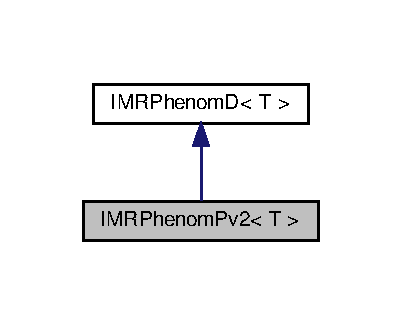
\includegraphics[width=252pt]{classIMRPhenomPv2__inherit__graph}
\end{center}
\end{figure}


Collaboration diagram for I\+M\+R\+Phenom\+Pv2$<$ T $>$\+:
\nopagebreak
\begin{figure}[H]
\begin{center}
\leavevmode
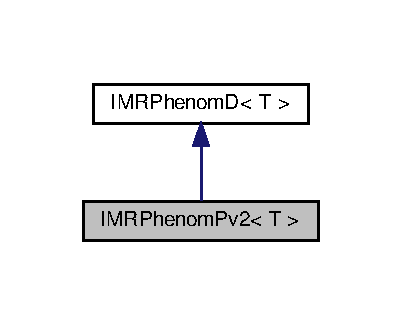
\includegraphics[width=193pt]{classIMRPhenomPv2__coll__graph}
\end{center}
\end{figure}
\doxysubsection*{Public Member Functions}
\begin{DoxyCompactItemize}
\item 
\mbox{\Hypertarget{classIMRPhenomPv2_ae3a484c9f30a94cde0fd996e164e1f7d}\label{classIMRPhenomPv2_ae3a484c9f30a94cde0fd996e164e1f7d}} 
virtual T {\bfseries alpha} (T omega, T q, T chi2l, T chi2)
\item 
\mbox{\Hypertarget{classIMRPhenomPv2_a5fff973809492fa59aff6d7d44a2b37a}\label{classIMRPhenomPv2_a5fff973809492fa59aff6d7d44a2b37a}} 
virtual T {\bfseries epsilon} (T omega, T q, T chi2l, T chi2)
\item 
virtual void \mbox{\hyperlink{classIMRPhenomPv2_afc0f88c773f46ab060482bc530f60115}{calculate\+\_\+euler\+\_\+coeffs}} (\mbox{\hyperlink{structalpha__coeffs}{alpha\+\_\+coeffs}}$<$ T $>$ $\ast$acoeffs, \mbox{\hyperlink{structepsilon__coeffs}{epsilon\+\_\+coeffs}}$<$ T $>$ $\ast$ecoeffs, \mbox{\hyperlink{structsource__parameters}{source\+\_\+parameters}}$<$ T $>$ $\ast$params)
\begin{DoxyCompactList}\small\item\em Pre calculate euler angle coefficients. \end{DoxyCompactList}\item 
\mbox{\Hypertarget{classIMRPhenomPv2_a61b485a13745066477875a4b192dd940}\label{classIMRPhenomPv2_a61b485a13745066477875a4b192dd940}} 
virtual T {\bfseries d} (int l, int mp, int m, T s)
\item 
virtual void \mbox{\hyperlink{classIMRPhenomPv2_a9c81435792ee35948b3e7b3438c1ef1e}{Phenom\+Pv2\+\_\+\+J\+S\+F\+\_\+from\+\_\+params}} (\mbox{\hyperlink{classgen__params__base}{gen\+\_\+params\+\_\+base}}$<$ T $>$ $\ast$params, T $\ast$J\+SF)
\begin{DoxyCompactList}\small\item\em Calculate the unit vector in the direction of the total angular momentum. \end{DoxyCompactList}\item 
virtual int \mbox{\hyperlink{classIMRPhenomPv2_af147bf8756311a9386b3f9bcdefa7dd5}{construct\+\_\+waveform}} (T $\ast$frequencies, int length, std\+::complex$<$ T $>$ $\ast$waveform\+\_\+plus, std\+::complex$<$ T $>$ $\ast$waveform\+\_\+cross, \mbox{\hyperlink{structsource__parameters}{source\+\_\+parameters}}$<$ T $>$ $\ast$params)
\begin{DoxyCompactList}\small\item\em Constructs the waveform for \mbox{\hyperlink{classIMRPhenomPv2}{I\+M\+R\+Phenom\+Pv2}} -\/ uses \mbox{\hyperlink{classIMRPhenomD}{I\+M\+R\+PhenomD}}, then twists up. \end{DoxyCompactList}\item 
virtual int \mbox{\hyperlink{classIMRPhenomPv2_a05877c187dedd47f2479939907b4b2e9}{construct\+\_\+phase}} (T $\ast$frequencies, int length, T $\ast$phase\+\_\+plus, T $\ast$phase\+\_\+cross, \mbox{\hyperlink{structsource__parameters}{source\+\_\+parameters}}$<$ T $>$ $\ast$params)
\begin{DoxyCompactList}\small\item\em Constructs the phase for \mbox{\hyperlink{classIMRPhenomPv2}{I\+M\+R\+Phenom\+Pv2}} -\/ uses \mbox{\hyperlink{classIMRPhenomD}{I\+M\+R\+PhenomD}}, then twists up. \end{DoxyCompactList}\item 
\mbox{\Hypertarget{classIMRPhenomPv2_a326eaa63c365113abfa37830f0a0f42f}\label{classIMRPhenomPv2_a326eaa63c365113abfa37830f0a0f42f}} 
virtual T {\bfseries calculate\+\_\+time\+\_\+shift} (\mbox{\hyperlink{structsource__parameters}{source\+\_\+parameters}}$<$ T $>$ $\ast$params, \mbox{\hyperlink{structuseful__powers}{useful\+\_\+powers}}$<$ T $>$ $\ast$pows, T $\ast$pn\+\_\+phase\+\_\+coeffs, \mbox{\hyperlink{structlambda__parameters}{lambda\+\_\+parameters}}$<$ T $>$ $\ast$lambda)
\item 
\mbox{\Hypertarget{classIMRPhenomPv2_abd66fb1738b26466d28d8f4050d4207c}\label{classIMRPhenomPv2_abd66fb1738b26466d28d8f4050d4207c}} 
virtual void {\bfseries WignerD} (T d2\mbox{[}5\mbox{]}, T dm2\mbox{[}5\mbox{]}, \mbox{\hyperlink{structuseful__powers}{useful\+\_\+powers}}$<$ T $>$ $\ast$pows, \mbox{\hyperlink{structsource__parameters}{source\+\_\+parameters}}$<$ T $>$ $\ast$params)
\item 
\mbox{\Hypertarget{classIMRPhenomPv2_a2f7dc5cbc5451036e15b7eaa3e170f96}\label{classIMRPhenomPv2_a2f7dc5cbc5451036e15b7eaa3e170f96}} 
virtual void {\bfseries calculate\+\_\+twistup} (T alpha, std\+::complex$<$ T $>$ $\ast$hp\+\_\+factor, std\+::complex$<$ T $>$ $\ast$hc\+\_\+factor, T d2\mbox{[}5\mbox{]}, T dm2\mbox{[}5\mbox{]}, \mbox{\hyperlink{structsph__harm}{sph\+\_\+harm}}$<$ T $>$ $\ast$\mbox{\hyperlink{structsph__harm}{sph\+\_\+harm}})
\item 
\mbox{\Hypertarget{classIMRPhenomPv2_aba929d7ceebe4ddbfd13088c1ac0596b}\label{classIMRPhenomPv2_aba929d7ceebe4ddbfd13088c1ac0596b}} 
virtual void {\bfseries calculate\+\_\+euler\+\_\+angles} (T $\ast$alpha, T $\ast$epsilon, \mbox{\hyperlink{structuseful__powers}{useful\+\_\+powers}}$<$ T $>$ $\ast$pows, \mbox{\hyperlink{structalpha__coeffs}{alpha\+\_\+coeffs}}$<$ T $>$ $\ast$acoeffs, \mbox{\hyperlink{structepsilon__coeffs}{epsilon\+\_\+coeffs}}$<$ T $>$ $\ast$ecoeffs)
\item 
virtual void \mbox{\hyperlink{classIMRPhenomPv2_ae8f253a1feebc43995dd5d052c856e05}{Phenom\+Pv2\+\_\+\+Param\+\_\+\+Transform}} (\mbox{\hyperlink{structsource__parameters}{source\+\_\+parameters}}$<$ T $>$ $\ast$params)
\item 
virtual void \mbox{\hyperlink{classIMRPhenomPv2_a684f1bbc22773a72e8000de61c1b6def}{Phenom\+Pv2\+\_\+\+Param\+\_\+\+Transform\+\_\+J}} (\mbox{\hyperlink{structsource__parameters}{source\+\_\+parameters}}$<$ T $>$ $\ast$params)
\item 
virtual void \mbox{\hyperlink{classIMRPhenomPv2_a09917aef3521bd8e3b8d8516930077a0}{Phenom\+Pv2\+\_\+\+Param\+\_\+\+Transform\+\_\+reduced}} (\mbox{\hyperlink{structsource__parameters}{source\+\_\+parameters}}$<$ T $>$ $\ast$params)
\item 
\mbox{\Hypertarget{classIMRPhenomPv2_a5e64520f828d29beccdf5b1e5e18582c}\label{classIMRPhenomPv2_a5e64520f828d29beccdf5b1e5e18582c}} 
virtual T {\bfseries L2\+PN} (T eta, \mbox{\hyperlink{structuseful__powers}{useful\+\_\+powers}}$<$ T $>$ $\ast$pow)
\item 
virtual T \mbox{\hyperlink{classIMRPhenomPv2_a36cbd07ab5b8c1663c7f8c8e75cf4e74}{Final\+Spin\+I\+M\+R\+Phenom\+D\+\_\+all\+\_\+in\+\_\+plane\+\_\+spin\+\_\+on\+\_\+larger\+\_\+\+BH}} (T m1, T m2, T chi1\+\_\+l, T chi2\+\_\+l, T chip)
\item 
\mbox{\Hypertarget{classIMRPhenomPv2_a3d37a40e4d1bce6ca673e6b30e64fe67}\label{classIMRPhenomPv2_a3d37a40e4d1bce6ca673e6b30e64fe67}} 
virtual T {\bfseries final\+\_\+spin} (\mbox{\hyperlink{structsource__parameters}{source\+\_\+parameters}}$<$ T $>$ $\ast$params)
\item 
{\footnotesize template$<$$>$ }\\double \mbox{\hyperlink{classIMRPhenomPv2_a6b27bd676726358b699a35cfbd10fe79}{calculate\+\_\+time\+\_\+shift}} (\mbox{\hyperlink{structsource__parameters}{source\+\_\+parameters}}$<$ double $>$ $\ast$params, \mbox{\hyperlink{structuseful__powers}{useful\+\_\+powers}}$<$ double $>$ $\ast$pows, double $\ast$pn\+\_\+phase\+\_\+coeffs, \mbox{\hyperlink{structlambda__parameters}{lambda\+\_\+parameters}}$<$ double $>$ $\ast$lambda)
\begin{DoxyCompactList}\small\item\em Shifts the time of coalescence to the desired value. \end{DoxyCompactList}\item 
{\footnotesize template$<$$>$ }\\adouble \mbox{\hyperlink{classIMRPhenomPv2_a61ec2bf7f72ec82b5a583e7098b2daab}{calculate\+\_\+time\+\_\+shift}} (\mbox{\hyperlink{structsource__parameters}{source\+\_\+parameters}}$<$ adouble $>$ $\ast$params, \mbox{\hyperlink{structuseful__powers}{useful\+\_\+powers}}$<$ adouble $>$ $\ast$pows, adouble $\ast$pn\+\_\+phase\+\_\+coeffs, \mbox{\hyperlink{structlambda__parameters}{lambda\+\_\+parameters}}$<$ adouble $>$ $\ast$lambda)
\begin{DoxyCompactList}\small\item\em Shifts the time of coalescence to the desired value. \end{DoxyCompactList}\end{DoxyCompactItemize}


\doxysubsection{Member Function Documentation}
\mbox{\Hypertarget{classIMRPhenomPv2_afc0f88c773f46ab060482bc530f60115}\label{classIMRPhenomPv2_afc0f88c773f46ab060482bc530f60115}} 
\index{IMRPhenomPv2$<$ T $>$@{IMRPhenomPv2$<$ T $>$}!calculate\_euler\_coeffs@{calculate\_euler\_coeffs}}
\index{calculate\_euler\_coeffs@{calculate\_euler\_coeffs}!IMRPhenomPv2$<$ T $>$@{IMRPhenomPv2$<$ T $>$}}
\doxysubsubsection{\texorpdfstring{calculate\_euler\_coeffs()}{calculate\_euler\_coeffs()}}
{\footnotesize\ttfamily template$<$class T $>$ \\
void \mbox{\hyperlink{classIMRPhenomPv2}{I\+M\+R\+Phenom\+Pv2}}$<$ T $>$\+::calculate\+\_\+euler\+\_\+coeffs (\begin{DoxyParamCaption}\item[{\mbox{\hyperlink{structalpha__coeffs}{alpha\+\_\+coeffs}}$<$ T $>$ $\ast$}]{acoeffs,  }\item[{\mbox{\hyperlink{structepsilon__coeffs}{epsilon\+\_\+coeffs}}$<$ T $>$ $\ast$}]{ecoeffs,  }\item[{\mbox{\hyperlink{structsource__parameters}{source\+\_\+parameters}}$<$ T $>$ $\ast$}]{params }\end{DoxyParamCaption})\hspace{0.3cm}{\ttfamily [virtual]}}



Pre calculate euler angle coefficients. 

Straight up stolen from L\+A\+Lsuite \mbox{\Hypertarget{classIMRPhenomPv2_a61ec2bf7f72ec82b5a583e7098b2daab}\label{classIMRPhenomPv2_a61ec2bf7f72ec82b5a583e7098b2daab}} 
\index{IMRPhenomPv2$<$ T $>$@{IMRPhenomPv2$<$ T $>$}!calculate\_time\_shift@{calculate\_time\_shift}}
\index{calculate\_time\_shift@{calculate\_time\_shift}!IMRPhenomPv2$<$ T $>$@{IMRPhenomPv2$<$ T $>$}}
\doxysubsubsection{\texorpdfstring{calculate\_time\_shift()}{calculate\_time\_shift()}\hspace{0.1cm}{\footnotesize\ttfamily [1/2]}}
{\footnotesize\ttfamily template$<$$>$ \\
adouble \mbox{\hyperlink{classIMRPhenomPv2}{I\+M\+R\+Phenom\+Pv2}}$<$ adouble $>$\+::calculate\+\_\+time\+\_\+shift (\begin{DoxyParamCaption}\item[{\mbox{\hyperlink{structsource__parameters}{source\+\_\+parameters}}$<$ adouble $>$ $\ast$}]{params,  }\item[{\mbox{\hyperlink{structuseful__powers}{useful\+\_\+powers}}$<$ adouble $>$ $\ast$}]{pows,  }\item[{adouble $\ast$}]{pn\+\_\+phase\+\_\+coeffs,  }\item[{\mbox{\hyperlink{structlambda__parameters}{lambda\+\_\+parameters}}$<$ adouble $>$ $\ast$}]{lambda }\end{DoxyParamCaption})}



Shifts the time of coalescence to the desired value. 

Because G\+SL interpolation must have double (not adouble), the two cases must behandled separately, explicitly. \mbox{\Hypertarget{classIMRPhenomPv2_a6b27bd676726358b699a35cfbd10fe79}\label{classIMRPhenomPv2_a6b27bd676726358b699a35cfbd10fe79}} 
\index{IMRPhenomPv2$<$ T $>$@{IMRPhenomPv2$<$ T $>$}!calculate\_time\_shift@{calculate\_time\_shift}}
\index{calculate\_time\_shift@{calculate\_time\_shift}!IMRPhenomPv2$<$ T $>$@{IMRPhenomPv2$<$ T $>$}}
\doxysubsubsection{\texorpdfstring{calculate\_time\_shift()}{calculate\_time\_shift()}\hspace{0.1cm}{\footnotesize\ttfamily [2/2]}}
{\footnotesize\ttfamily template$<$$>$ \\
double \mbox{\hyperlink{classIMRPhenomPv2}{I\+M\+R\+Phenom\+Pv2}}$<$ double $>$\+::calculate\+\_\+time\+\_\+shift (\begin{DoxyParamCaption}\item[{\mbox{\hyperlink{structsource__parameters}{source\+\_\+parameters}}$<$ double $>$ $\ast$}]{params,  }\item[{\mbox{\hyperlink{structuseful__powers}{useful\+\_\+powers}}$<$ double $>$ $\ast$}]{pows,  }\item[{double $\ast$}]{pn\+\_\+phase\+\_\+coeffs,  }\item[{\mbox{\hyperlink{structlambda__parameters}{lambda\+\_\+parameters}}$<$ double $>$ $\ast$}]{lambda }\end{DoxyParamCaption})}



Shifts the time of coalescence to the desired value. 

Because G\+SL interpolation must have double (not adouble), the two cases must behandled separately, explicitly. \mbox{\Hypertarget{classIMRPhenomPv2_a05877c187dedd47f2479939907b4b2e9}\label{classIMRPhenomPv2_a05877c187dedd47f2479939907b4b2e9}} 
\index{IMRPhenomPv2$<$ T $>$@{IMRPhenomPv2$<$ T $>$}!construct\_phase@{construct\_phase}}
\index{construct\_phase@{construct\_phase}!IMRPhenomPv2$<$ T $>$@{IMRPhenomPv2$<$ T $>$}}
\doxysubsubsection{\texorpdfstring{construct\_phase()}{construct\_phase()}}
{\footnotesize\ttfamily template$<$class T $>$ \\
int \mbox{\hyperlink{classIMRPhenomPv2}{I\+M\+R\+Phenom\+Pv2}}$<$ T $>$\+::construct\+\_\+phase (\begin{DoxyParamCaption}\item[{T $\ast$}]{frequencies,  }\item[{int}]{length,  }\item[{T $\ast$}]{phase\+\_\+plus,  }\item[{T $\ast$}]{phase\+\_\+cross,  }\item[{\mbox{\hyperlink{structsource__parameters}{source\+\_\+parameters}}$<$ T $>$ $\ast$}]{params }\end{DoxyParamCaption})\hspace{0.3cm}{\ttfamily [virtual]}}



Constructs the phase for \mbox{\hyperlink{classIMRPhenomPv2}{I\+M\+R\+Phenom\+Pv2}} -\/ uses \mbox{\hyperlink{classIMRPhenomD}{I\+M\+R\+PhenomD}}, then twists up. 

arguments\+: array of frequencies, length of that array, a complex array for the output waveform, and a \mbox{\hyperlink{structsource__parameters}{source\+\_\+parameters}} structure 
\begin{DoxyParams}{Parameters}
{\em frequencies} & T array of frequencies the waveform is to be evaluated at \\
\hline
{\em length} & integer length of the array of frequencies and the waveform \\
\hline
{\em phase\+\_\+plus} & complex T array for the plus polariaztion waveform to be output \\
\hline
{\em phase\+\_\+cross} & complex T array for the cross polarization waveform to be output \\
\hline
\end{DoxyParams}
\mbox{\Hypertarget{classIMRPhenomPv2_af147bf8756311a9386b3f9bcdefa7dd5}\label{classIMRPhenomPv2_af147bf8756311a9386b3f9bcdefa7dd5}} 
\index{IMRPhenomPv2$<$ T $>$@{IMRPhenomPv2$<$ T $>$}!construct\_waveform@{construct\_waveform}}
\index{construct\_waveform@{construct\_waveform}!IMRPhenomPv2$<$ T $>$@{IMRPhenomPv2$<$ T $>$}}
\doxysubsubsection{\texorpdfstring{construct\_waveform()}{construct\_waveform()}}
{\footnotesize\ttfamily template$<$class T $>$ \\
int \mbox{\hyperlink{classIMRPhenomPv2}{I\+M\+R\+Phenom\+Pv2}}$<$ T $>$\+::construct\+\_\+waveform (\begin{DoxyParamCaption}\item[{T $\ast$}]{frequencies,  }\item[{int}]{length,  }\item[{std\+::complex$<$ T $>$ $\ast$}]{waveform\+\_\+plus,  }\item[{std\+::complex$<$ T $>$ $\ast$}]{waveform\+\_\+cross,  }\item[{\mbox{\hyperlink{structsource__parameters}{source\+\_\+parameters}}$<$ T $>$ $\ast$}]{params }\end{DoxyParamCaption})\hspace{0.3cm}{\ttfamily [virtual]}}



Constructs the waveform for \mbox{\hyperlink{classIMRPhenomPv2}{I\+M\+R\+Phenom\+Pv2}} -\/ uses \mbox{\hyperlink{classIMRPhenomD}{I\+M\+R\+PhenomD}}, then twists up. 

arguments\+: array of frequencies, length of that array, a complex array for the output waveform, and a \mbox{\hyperlink{structsource__parameters}{source\+\_\+parameters}} structure 
\begin{DoxyParams}{Parameters}
{\em frequencies} & T array of frequencies the waveform is to be evaluated at \\
\hline
{\em length} & integer length of the array of frequencies and the waveform \\
\hline
{\em waveform\+\_\+plus} & complex T array for the plus polariaztion waveform to be output \\
\hline
{\em waveform\+\_\+cross} & complex T array for the cross polarization waveform to be output \\
\hline
\end{DoxyParams}
\mbox{\Hypertarget{classIMRPhenomPv2_a36cbd07ab5b8c1663c7f8c8e75cf4e74}\label{classIMRPhenomPv2_a36cbd07ab5b8c1663c7f8c8e75cf4e74}} 
\index{IMRPhenomPv2$<$ T $>$@{IMRPhenomPv2$<$ T $>$}!FinalSpinIMRPhenomD\_all\_in\_plane\_spin\_on\_larger\_BH@{FinalSpinIMRPhenomD\_all\_in\_plane\_spin\_on\_larger\_BH}}
\index{FinalSpinIMRPhenomD\_all\_in\_plane\_spin\_on\_larger\_BH@{FinalSpinIMRPhenomD\_all\_in\_plane\_spin\_on\_larger\_BH}!IMRPhenomPv2$<$ T $>$@{IMRPhenomPv2$<$ T $>$}}
\doxysubsubsection{\texorpdfstring{FinalSpinIMRPhenomD\_all\_in\_plane\_spin\_on\_larger\_BH()}{FinalSpinIMRPhenomD\_all\_in\_plane\_spin\_on\_larger\_BH()}}
{\footnotesize\ttfamily template$<$class T $>$ \\
T \mbox{\hyperlink{classIMRPhenomPv2}{I\+M\+R\+Phenom\+Pv2}}$<$ T $>$\+::Final\+Spin\+I\+M\+R\+Phenom\+D\+\_\+all\+\_\+in\+\_\+plane\+\_\+spin\+\_\+on\+\_\+larger\+\_\+\+BH (\begin{DoxyParamCaption}\item[{T}]{m1,  }\item[{T}]{m2,  }\item[{T}]{chi1\+\_\+l,  }\item[{T}]{chi2\+\_\+l,  }\item[{T}]{chip }\end{DoxyParamCaption})\hspace{0.3cm}{\ttfamily [virtual]}}


\begin{DoxyItemize}
\item Wrapper for final-\/spin formula based on\+:
\begin{DoxyItemize}
\item -\/ \mbox{\hyperlink{classIMRPhenomD}{I\+M\+R\+PhenomD}}\textquotesingle{}s \mbox{\hyperlink{classIMRPhenomD_af638fe3433f2367f9dfe6e2236a6b0ee}{Final\+Spin0815()}} for aligned spins.
\begin{DoxyItemize}
\item 
\begin{DoxyItemize}
\item We use their convention m1$>$m2
\begin{DoxyItemize}
\item and put {\bfseries{all in-\/plane spin on the larger BH}}.
\begin{DoxyItemize}
\item 
\begin{DoxyItemize}
\item In the aligned limit return the Final\+Spin0815 value. 
\end{DoxyItemize}
\end{DoxyItemize}
\end{DoxyItemize}
\end{DoxyItemize}
\end{DoxyItemize}
\end{DoxyItemize}
\end{DoxyItemize}
\begin{DoxyParams}{Parameters}
{\em m1} & Mass of companion 1 (solar masses) \\
\hline
{\em m2} & Mass of companion 2 (solar masses) \\
\hline
{\em chi1\+\_\+l} & Aligned spin of BH 1 \\
\hline
{\em chi2\+\_\+l} & Aligned spin of BH 2 \\
\hline
{\em chip} & Dimensionless spin in the orbital plane \\
\hline
\end{DoxyParams}
\mbox{\Hypertarget{classIMRPhenomPv2_a9c81435792ee35948b3e7b3438c1ef1e}\label{classIMRPhenomPv2_a9c81435792ee35948b3e7b3438c1ef1e}} 
\index{IMRPhenomPv2$<$ T $>$@{IMRPhenomPv2$<$ T $>$}!PhenomPv2\_JSF\_from\_params@{PhenomPv2\_JSF\_from\_params}}
\index{PhenomPv2\_JSF\_from\_params@{PhenomPv2\_JSF\_from\_params}!IMRPhenomPv2$<$ T $>$@{IMRPhenomPv2$<$ T $>$}}
\doxysubsubsection{\texorpdfstring{PhenomPv2\_JSF\_from\_params()}{PhenomPv2\_JSF\_from\_params()}}
{\footnotesize\ttfamily template$<$class T $>$ \\
void \mbox{\hyperlink{classIMRPhenomPv2}{I\+M\+R\+Phenom\+Pv2}}$<$ T $>$\+::Phenom\+Pv2\+\_\+\+J\+S\+F\+\_\+from\+\_\+params (\begin{DoxyParamCaption}\item[{\mbox{\hyperlink{classgen__params__base}{gen\+\_\+params\+\_\+base}}$<$ T $>$ $\ast$}]{params,  }\item[{T $\ast$}]{J\+SF }\end{DoxyParamCaption})\hspace{0.3cm}{\ttfamily [virtual]}}



Calculate the unit vector in the direction of the total angular momentum. 

\mbox{\Hypertarget{classIMRPhenomPv2_ae8f253a1feebc43995dd5d052c856e05}\label{classIMRPhenomPv2_ae8f253a1feebc43995dd5d052c856e05}} 
\index{IMRPhenomPv2$<$ T $>$@{IMRPhenomPv2$<$ T $>$}!PhenomPv2\_Param\_Transform@{PhenomPv2\_Param\_Transform}}
\index{PhenomPv2\_Param\_Transform@{PhenomPv2\_Param\_Transform}!IMRPhenomPv2$<$ T $>$@{IMRPhenomPv2$<$ T $>$}}
\doxysubsubsection{\texorpdfstring{PhenomPv2\_Param\_Transform()}{PhenomPv2\_Param\_Transform()}}
{\footnotesize\ttfamily template$<$class T $>$ \\
void \mbox{\hyperlink{classIMRPhenomPv2}{I\+M\+R\+Phenom\+Pv2}}$<$ T $>$\+::Phenom\+Pv2\+\_\+\+Param\+\_\+\+Transform (\begin{DoxyParamCaption}\item[{\mbox{\hyperlink{structsource__parameters}{source\+\_\+parameters}}$<$ T $>$ $\ast$}]{params }\end{DoxyParamCaption})\hspace{0.3cm}{\ttfamily [virtual]}}

/\+Brief Parameter transformtion to precalculate needed parameters for PhenomP from source parameters

Pretty much stolen verbatim from lalsuite \mbox{\Hypertarget{classIMRPhenomPv2_a684f1bbc22773a72e8000de61c1b6def}\label{classIMRPhenomPv2_a684f1bbc22773a72e8000de61c1b6def}} 
\index{IMRPhenomPv2$<$ T $>$@{IMRPhenomPv2$<$ T $>$}!PhenomPv2\_Param\_Transform\_J@{PhenomPv2\_Param\_Transform\_J}}
\index{PhenomPv2\_Param\_Transform\_J@{PhenomPv2\_Param\_Transform\_J}!IMRPhenomPv2$<$ T $>$@{IMRPhenomPv2$<$ T $>$}}
\doxysubsubsection{\texorpdfstring{PhenomPv2\_Param\_Transform\_J()}{PhenomPv2\_Param\_Transform\_J()}}
{\footnotesize\ttfamily template$<$class T $>$ \\
void \mbox{\hyperlink{classIMRPhenomPv2}{I\+M\+R\+Phenom\+Pv2}}$<$ T $>$\+::Phenom\+Pv2\+\_\+\+Param\+\_\+\+Transform\+\_\+J (\begin{DoxyParamCaption}\item[{\mbox{\hyperlink{structsource__parameters}{source\+\_\+parameters}}$<$ T $>$ $\ast$}]{params }\end{DoxyParamCaption})\hspace{0.3cm}{\ttfamily [virtual]}}

/\+Brief Parameter transformtion to precalculate needed parameters for PhenomP from source parameters -- assumed inclination of total angular momentum J is given, not orbital angular momentum (in source frame (Lhat == zhat)

Pretty much stolen verbatim from lalsuite \mbox{\Hypertarget{classIMRPhenomPv2_a09917aef3521bd8e3b8d8516930077a0}\label{classIMRPhenomPv2_a09917aef3521bd8e3b8d8516930077a0}} 
\index{IMRPhenomPv2$<$ T $>$@{IMRPhenomPv2$<$ T $>$}!PhenomPv2\_Param\_Transform\_reduced@{PhenomPv2\_Param\_Transform\_reduced}}
\index{PhenomPv2\_Param\_Transform\_reduced@{PhenomPv2\_Param\_Transform\_reduced}!IMRPhenomPv2$<$ T $>$@{IMRPhenomPv2$<$ T $>$}}
\doxysubsubsection{\texorpdfstring{PhenomPv2\_Param\_Transform\_reduced()}{PhenomPv2\_Param\_Transform\_reduced()}}
{\footnotesize\ttfamily template$<$class T $>$ \\
void \mbox{\hyperlink{classIMRPhenomPv2}{I\+M\+R\+Phenom\+Pv2}}$<$ T $>$\+::Phenom\+Pv2\+\_\+\+Param\+\_\+\+Transform\+\_\+reduced (\begin{DoxyParamCaption}\item[{\mbox{\hyperlink{structsource__parameters}{source\+\_\+parameters}}$<$ T $>$ $\ast$}]{params }\end{DoxyParamCaption})\hspace{0.3cm}{\ttfamily [virtual]}}

/\+Brief Parameter transformation to pre-\/calculate needed parameters for PhenomP from source parameters

Pretty much stolen verbatim from lalsuite 

The documentation for this class was generated from the following files\+:\begin{DoxyCompactItemize}
\item 
include/gwat/\mbox{\hyperlink{IMRPhenomP_8h}{I\+M\+R\+Phenom\+P.\+h}}\item 
src/\mbox{\hyperlink{IMRPhenomP_8cpp}{I\+M\+R\+Phenom\+P.\+cpp}}\end{DoxyCompactItemize}

\hypertarget{structlambda__parameters}{}\section{lambda\+\_\+parameters$<$ T $>$ Struct Template Reference}
\label{structlambda__parameters}\index{lambda\+\_\+parameters$<$ T $>$@{lambda\+\_\+parameters$<$ T $>$}}


Collaboration diagram for lambda\+\_\+parameters$<$ T $>$\+:\nopagebreak
\begin{figure}[H]
\begin{center}
\leavevmode
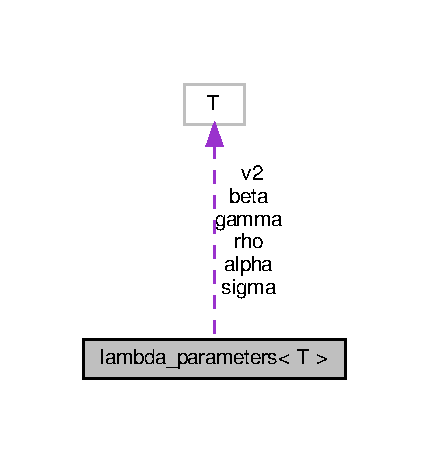
\includegraphics[width=206pt]{structlambda__parameters__coll__graph}
\end{center}
\end{figure}
\subsection*{Public Attributes}
\begin{DoxyCompactItemize}
\item 
\mbox{\Hypertarget{structlambda__parameters_a08f293753fe41b88fdd8a206b593a6c8}\label{structlambda__parameters_a08f293753fe41b88fdd8a206b593a6c8}} 
T {\bfseries rho} \mbox{[}4\mbox{]}
\item 
\mbox{\Hypertarget{structlambda__parameters_a35ec87e1f27de9393a6e94d18cd63c52}\label{structlambda__parameters_a35ec87e1f27de9393a6e94d18cd63c52}} 
T {\bfseries v2}
\item 
\mbox{\Hypertarget{structlambda__parameters_a49db18626c20bd43f25c5c760679ac2a}\label{structlambda__parameters_a49db18626c20bd43f25c5c760679ac2a}} 
T {\bfseries gamma} \mbox{[}4\mbox{]}
\item 
\mbox{\Hypertarget{structlambda__parameters_aefdccc025bcb819ec4b8009b232cf9b2}\label{structlambda__parameters_aefdccc025bcb819ec4b8009b232cf9b2}} 
T {\bfseries sigma} \mbox{[}5\mbox{]}
\item 
\mbox{\Hypertarget{structlambda__parameters_a4aa387f5a44b09541304c5e2f8f3aad6}\label{structlambda__parameters_a4aa387f5a44b09541304c5e2f8f3aad6}} 
T {\bfseries beta} \mbox{[}5\mbox{]}
\item 
\mbox{\Hypertarget{structlambda__parameters_aec862d891bc928fb1faf042aff322802}\label{structlambda__parameters_aec862d891bc928fb1faf042aff322802}} 
T {\bfseries alpha} \mbox{[}7\mbox{]}
\end{DoxyCompactItemize}


The documentation for this struct was generated from the following file\+:\begin{DoxyCompactItemize}
\item 
include/gwat/\hyperlink{IMRPhenomD_8h}{I\+M\+R\+Phenom\+D.\+h}\end{DoxyCompactItemize}

\hypertarget{structmcr__job}{}\section{mcr\+\_\+job Struct Reference}
\label{structmcr__job}\index{mcr\+\_\+job@{mcr\+\_\+job}}


Collaboration diagram for mcr\+\_\+job\+:\nopagebreak
\begin{figure}[H]
\begin{center}
\leavevmode
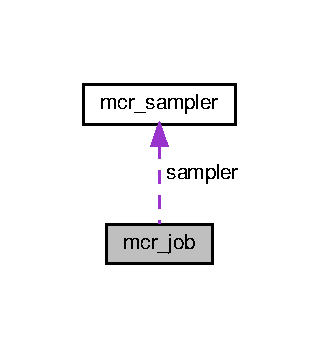
\includegraphics[width=155pt]{structmcr__job__coll__graph}
\end{center}
\end{figure}
\subsection*{Public Attributes}
\begin{DoxyCompactItemize}
\item 
\mbox{\Hypertarget{structmcr__job_a8016c242228440211dd8e0fdfd8cb1f7}\label{structmcr__job_a8016c242228440211dd8e0fdfd8cb1f7}} 
\hyperlink{classmcr__sampler}{mcr\+\_\+sampler} $\ast$ {\bfseries sampler}
\item 
\mbox{\Hypertarget{structmcr__job_a6f2dd320a49729257b6d075e1cce4e23}\label{structmcr__job_a6f2dd320a49729257b6d075e1cce4e23}} 
int {\bfseries starting\+\_\+index} =0
\item 
\mbox{\Hypertarget{structmcr__job_a590d489d391127ad426893819e37c671}\label{structmcr__job_a590d489d391127ad426893819e37c671}} 
int {\bfseries job\+\_\+length} =0
\item 
\mbox{\Hypertarget{structmcr__job_a027d799fdf34fb5aaa60d3c801b31cab}\label{structmcr__job_a027d799fdf34fb5aaa60d3c801b31cab}} 
void $\ast$$\ast$ {\bfseries output}
\end{DoxyCompactItemize}


The documentation for this struct was generated from the following file\+:\begin{DoxyCompactItemize}
\item 
include/gwat/\hyperlink{mc__reject_8h}{mc\+\_\+reject.\+h}\end{DoxyCompactItemize}

\hypertarget{classmcr__sampler}{}\section{mcr\+\_\+sampler Class Reference}
\label{classmcr__sampler}\index{mcr\+\_\+sampler@{mcr\+\_\+sampler}}
\subsection*{Public Member Functions}
\begin{DoxyCompactItemize}
\item 
\hyperlink{classmcr__sampler_a9f9da59f2b90a771e1fcd659aedbf920}{mcr\+\_\+sampler} (void($\ast$probability)(double $\ast$prob, void $\ast$parameters, int d, int threadid), void($\ast$draw\+\_\+parameters)(void $\ast$prop\+\_\+parameters, int d, int threadid, gsl\+\_\+rng $\ast$r), int dimension, double $\ast$param\+\_\+ranges\+\_\+max, double $\ast$param\+\_\+ranges\+\_\+min)
\begin{DoxyCompactList}\small\item\em Class constructor for Monte Carlo Rejection Sampler. \end{DoxyCompactList}\item 
\hyperlink{classmcr__sampler_a180f9fed263d2a277185a57604e85dd4}{mcr\+\_\+sampler} (void($\ast$probability)(double $\ast$prob, void $\ast$parameters, int d, int threadid), void($\ast$draw\+\_\+parameters)(void $\ast$prop\+\_\+parameters, int d, int threadid, gsl\+\_\+rng $\ast$r), int dimension, double $\ast$param\+\_\+ranges\+\_\+max, double $\ast$param\+\_\+ranges\+\_\+min, int thread\+\_\+num, bool thread\+\_\+safe)
\begin{DoxyCompactList}\small\item\em Class constructor for Monte Carlo Rejection Sampler. \end{DoxyCompactList}\item 
\hyperlink{classmcr__sampler_af1dc1bfe87a15819731e8082751ae224}{$\sim$mcr\+\_\+sampler} ()
\begin{DoxyCompactList}\small\item\em Destructor function for \hyperlink{classmcr__sampler}{mcr\+\_\+sampler}. \end{DoxyCompactList}\item 
void \hyperlink{classmcr__sampler_a5ba6b047e2f5cb8df12dcf593f3eb45e}{sample\+\_\+distribution} (int N\+\_\+samples, void $\ast$$\ast$output)
\begin{DoxyCompactList}\small\item\em Main driver -- Samples from distribution that has been associated with a sampler object. \end{DoxyCompactList}\item 
void \hyperlink{classmcr__sampler_a7127ccf1f0f385b6bb9acbe5d5244990}{sample} (void $\ast$output, int threadid)
\begin{DoxyCompactList}\small\item\em Internal routine to return one accepted sample. \end{DoxyCompactList}\end{DoxyCompactItemize}
\subsection*{Public Attributes}
\begin{DoxyCompactItemize}
\item 
\mbox{\Hypertarget{classmcr__sampler_a8ea0db12646c21e02f99a22e8c69f287}\label{classmcr__sampler_a8ea0db12646c21e02f99a22e8c69f287}} 
bool {\bfseries thread\+\_\+safe}
\item 
\mbox{\Hypertarget{classmcr__sampler_a01cdfa4fd6116570b83bf9c00dffb4f2}\label{classmcr__sampler_a01cdfa4fd6116570b83bf9c00dffb4f2}} 
int {\bfseries thread\+\_\+num}
\item 
\mbox{\Hypertarget{classmcr__sampler_a6316178e63a7e2fd07c3cc74b14a986d}\label{classmcr__sampler_a6316178e63a7e2fd07c3cc74b14a986d}} 
int {\bfseries dimension}
\item 
\mbox{\Hypertarget{classmcr__sampler_af8f92c143d75d35fae0714ec955b81b9}\label{classmcr__sampler_af8f92c143d75d35fae0714ec955b81b9}} 
int {\bfseries parallel\+\_\+job\+\_\+num}
\item 
\mbox{\Hypertarget{classmcr__sampler_a962ef98523fcd354b538175f335baf58}\label{classmcr__sampler_a962ef98523fcd354b538175f335baf58}} 
double $\ast$ {\bfseries param\+\_\+ranges\+\_\+max}
\item 
\mbox{\Hypertarget{classmcr__sampler_a99855b66f70b2fbea2458aa4046088e8}\label{classmcr__sampler_a99855b66f70b2fbea2458aa4046088e8}} 
double $\ast$ {\bfseries param\+\_\+ranges\+\_\+min}
\item 
\mbox{\Hypertarget{classmcr__sampler_ad87f2d7738158ed37629c34336b0aa60}\label{classmcr__sampler_ad87f2d7738158ed37629c34336b0aa60}} 
std\+::function$<$ void(double $\ast$, void $\ast$, int, int)$>$ {\bfseries pfn}
\item 
\mbox{\Hypertarget{classmcr__sampler_a48e9c96d43b1bb2cf912383cf642f3a7}\label{classmcr__sampler_a48e9c96d43b1bb2cf912383cf642f3a7}} 
std\+::function$<$ void(void $\ast$, int, int, gsl\+\_\+rng $\ast$)$>$ {\bfseries draw\+\_\+param}
\item 
\mbox{\Hypertarget{classmcr__sampler_aedb26b1163d8705bf64af08867a72d20}\label{classmcr__sampler_aedb26b1163d8705bf64af08867a72d20}} 
double $\ast$$\ast$ {\bfseries samples}
\end{DoxyCompactItemize}


\subsection{Constructor \& Destructor Documentation}
\mbox{\Hypertarget{classmcr__sampler_a9f9da59f2b90a771e1fcd659aedbf920}\label{classmcr__sampler_a9f9da59f2b90a771e1fcd659aedbf920}} 
\index{mcr\+\_\+sampler@{mcr\+\_\+sampler}!mcr\+\_\+sampler@{mcr\+\_\+sampler}}
\index{mcr\+\_\+sampler@{mcr\+\_\+sampler}!mcr\+\_\+sampler@{mcr\+\_\+sampler}}
\subsubsection{\texorpdfstring{mcr\+\_\+sampler()}{mcr\_sampler()}\hspace{0.1cm}{\footnotesize\ttfamily [1/2]}}
{\footnotesize\ttfamily mcr\+\_\+sampler\+::mcr\+\_\+sampler (\begin{DoxyParamCaption}\item[{void($\ast$)(double $\ast$prob, void $\ast$parameters, int d, int threadid)}]{probability,  }\item[{void($\ast$)(void $\ast$prop\+\_\+parameters, int d, int threadid, gsl\+\_\+rng $\ast$r)}]{draw\+\_\+parameters,  }\item[{int}]{dimension,  }\item[{double $\ast$}]{param\+\_\+ranges\+\_\+max,  }\item[{double $\ast$}]{param\+\_\+ranges\+\_\+min }\end{DoxyParamCaption})}



Class constructor for Monte Carlo Rejection Sampler. 

Assumes no parallel threading

``probability\textquotesingle{}\textquotesingle{} is the function that should return the probability of a given sample

``draw\+\_\+parameters\textquotesingle{}\textquotesingle{} -- N\+U\+LL, if default should be used. Otherwise, this should propose another parameter set

param\+\_\+ranges\+\_\+max/min are only used if the default draw\+\_\+parameter is used, otherwise can be N\+U\+LL 
\begin{DoxyParams}{Parameters}
{\em dimension} & Dimension \\
\hline
{\em param\+\_\+ranges\+\_\+max} & Max allowed parameters -- Shape \mbox{[}dimension\mbox{]} \\
\hline
{\em param\+\_\+ranges\+\_\+min} & Min allowed parameters -- Shape \mbox{[}dimension\mbox{]} \\
\hline
\end{DoxyParams}
\mbox{\Hypertarget{classmcr__sampler_a180f9fed263d2a277185a57604e85dd4}\label{classmcr__sampler_a180f9fed263d2a277185a57604e85dd4}} 
\index{mcr\+\_\+sampler@{mcr\+\_\+sampler}!mcr\+\_\+sampler@{mcr\+\_\+sampler}}
\index{mcr\+\_\+sampler@{mcr\+\_\+sampler}!mcr\+\_\+sampler@{mcr\+\_\+sampler}}
\subsubsection{\texorpdfstring{mcr\+\_\+sampler()}{mcr\_sampler()}\hspace{0.1cm}{\footnotesize\ttfamily [2/2]}}
{\footnotesize\ttfamily mcr\+\_\+sampler\+::mcr\+\_\+sampler (\begin{DoxyParamCaption}\item[{void($\ast$)(double $\ast$prob, void $\ast$parameters, int d, int threadid)}]{probability,  }\item[{void($\ast$)(void $\ast$prop\+\_\+parameters, int d, int threadid, gsl\+\_\+rng $\ast$r)}]{draw\+\_\+parameters,  }\item[{int}]{dimension,  }\item[{double $\ast$}]{param\+\_\+ranges\+\_\+max,  }\item[{double $\ast$}]{param\+\_\+ranges\+\_\+min,  }\item[{int}]{thread\+\_\+num,  }\item[{bool}]{thread\+\_\+safe }\end{DoxyParamCaption})}



Class constructor for Monte Carlo Rejection Sampler. 

Allows parallel threading

``probability\textquotesingle{}\textquotesingle{} is the function that should return the probability of a given sample

``draw\+\_\+parameters\textquotesingle{}\textquotesingle{} -- N\+U\+LL, if default should be used. Otherwise, this should propose another parameter set

param\+\_\+ranges\+\_\+max/min are only used if the default draw\+\_\+parameter is used, otherwise can be N\+U\+LL 
\begin{DoxyParams}{Parameters}
{\em dimension} & Dimension \\
\hline
{\em param\+\_\+ranges\+\_\+max} & Max allowed parameters -- Shape \mbox{[}dimension\mbox{]} \\
\hline
{\em param\+\_\+ranges\+\_\+min} & Min allowed parameters -- Shape \mbox{[}dimension\mbox{]} \\
\hline
{\em thread\+\_\+num} & Thread number to use \\
\hline
{\em thread\+\_\+safe} & Bool thread safe -- true if parallel threading should be used \\
\hline
\end{DoxyParams}
\mbox{\Hypertarget{classmcr__sampler_af1dc1bfe87a15819731e8082751ae224}\label{classmcr__sampler_af1dc1bfe87a15819731e8082751ae224}} 
\index{mcr\+\_\+sampler@{mcr\+\_\+sampler}!````~mcr\+\_\+sampler@{$\sim$mcr\+\_\+sampler}}
\index{````~mcr\+\_\+sampler@{$\sim$mcr\+\_\+sampler}!mcr\+\_\+sampler@{mcr\+\_\+sampler}}
\subsubsection{\texorpdfstring{$\sim$mcr\+\_\+sampler()}{~mcr\_sampler()}}
{\footnotesize\ttfamily mcr\+\_\+sampler\+::$\sim$mcr\+\_\+sampler (\begin{DoxyParamCaption}{ }\end{DoxyParamCaption})}



Destructor function for \hyperlink{classmcr__sampler}{mcr\+\_\+sampler}. 

Deallocates the gsl\+\_\+rng memory 

\subsection{Member Function Documentation}
\mbox{\Hypertarget{classmcr__sampler_a7127ccf1f0f385b6bb9acbe5d5244990}\label{classmcr__sampler_a7127ccf1f0f385b6bb9acbe5d5244990}} 
\index{mcr\+\_\+sampler@{mcr\+\_\+sampler}!sample@{sample}}
\index{sample@{sample}!mcr\+\_\+sampler@{mcr\+\_\+sampler}}
\subsubsection{\texorpdfstring{sample()}{sample()}}
{\footnotesize\ttfamily void mcr\+\_\+sampler\+::sample (\begin{DoxyParamCaption}\item[{void $\ast$}]{output,  }\item[{int}]{threadid }\end{DoxyParamCaption})}



Internal routine to return one accepted sample. 

Should not be used directly by user -- couldn\textquotesingle{}t make private though 
\begin{DoxyParams}[1]{Parameters}
\mbox{\tt out}  & {\em output} & Output, accepted parameter set \\
\hline
 & {\em threadid} & Thread id -- not currently used, but included for future proofing \\
\hline
\end{DoxyParams}
\mbox{\Hypertarget{classmcr__sampler_a5ba6b047e2f5cb8df12dcf593f3eb45e}\label{classmcr__sampler_a5ba6b047e2f5cb8df12dcf593f3eb45e}} 
\index{mcr\+\_\+sampler@{mcr\+\_\+sampler}!sample\+\_\+distribution@{sample\+\_\+distribution}}
\index{sample\+\_\+distribution@{sample\+\_\+distribution}!mcr\+\_\+sampler@{mcr\+\_\+sampler}}
\subsubsection{\texorpdfstring{sample\+\_\+distribution()}{sample\_distribution()}}
{\footnotesize\ttfamily void mcr\+\_\+sampler\+::sample\+\_\+distribution (\begin{DoxyParamCaption}\item[{int}]{N\+\_\+samples,  }\item[{void $\ast$$\ast$}]{output }\end{DoxyParamCaption})}



Main driver -- Samples from distribution that has been associated with a sampler object. 


\begin{DoxyParams}[1]{Parameters}
\mbox{\tt out}  & {\em output} & Output array shape \mbox{[}N\+\_\+samples\mbox{]}\mbox{[}dimension\mbox{]} Caste to void $\ast$$\ast$ \\
\hline
\end{DoxyParams}


The documentation for this class was generated from the following files\+:\begin{DoxyCompactItemize}
\item 
include/gwat/\hyperlink{mc__reject_8h}{mc\+\_\+reject.\+h}\item 
src/\hyperlink{mc__reject_8cpp}{mc\+\_\+reject.\+cpp}\end{DoxyCompactItemize}

\hypertarget{classppE__IMRPhenomD__IMR}{}\doxysection{pp\+E\+\_\+\+I\+M\+R\+Phenom\+D\+\_\+\+I\+MR$<$ T $>$ Class Template Reference}
\label{classppE__IMRPhenomD__IMR}\index{ppE\_IMRPhenomD\_IMR$<$ T $>$@{ppE\_IMRPhenomD\_IMR$<$ T $>$}}


{\ttfamily \#include $<$pp\+E\+\_\+\+I\+M\+R\+Phenom\+D.\+h$>$}



Inheritance diagram for pp\+E\+\_\+\+I\+M\+R\+Phenom\+D\+\_\+\+I\+MR$<$ T $>$\+:
\nopagebreak
\begin{figure}[H]
\begin{center}
\leavevmode
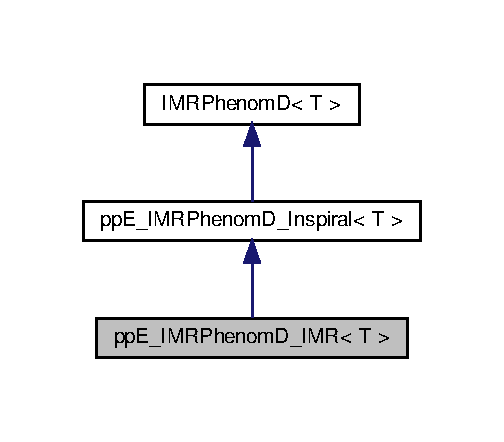
\includegraphics[width=242pt]{classppE__IMRPhenomD__IMR__inherit__graph}
\end{center}
\end{figure}


Collaboration diagram for pp\+E\+\_\+\+I\+M\+R\+Phenom\+D\+\_\+\+I\+MR$<$ T $>$\+:
\nopagebreak
\begin{figure}[H]
\begin{center}
\leavevmode
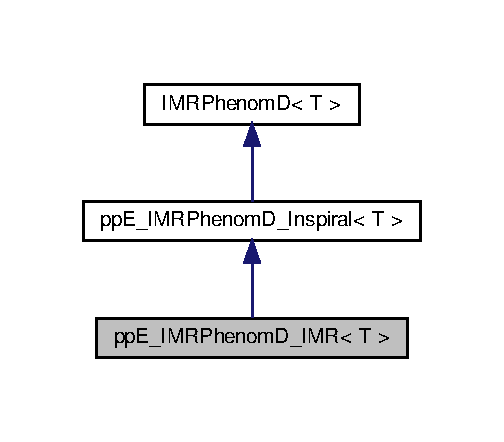
\includegraphics[width=242pt]{classppE__IMRPhenomD__IMR__coll__graph}
\end{center}
\end{figure}
\doxysubsection*{Public Member Functions}
\begin{DoxyCompactItemize}
\item 
virtual T \mbox{\hyperlink{classppE__IMRPhenomD__IMR_a3fa643eca535e7bef26f70bd5ed4cbde}{Dphase\+\_\+mr}} (T f, \mbox{\hyperlink{structsource__parameters}{source\+\_\+parameters}}$<$ T $>$ $\ast$param, \mbox{\hyperlink{structlambda__parameters}{lambda\+\_\+parameters}}$<$ T $>$ $\ast$lambda)
\begin{DoxyCompactList}\small\item\em Calculates the derivative of the merger-\/ringdown phase for frequency f. \end{DoxyCompactList}\item 
virtual T \mbox{\hyperlink{classppE__IMRPhenomD__IMR_a3b64e9bbf566450687bcfaa85c0e493f}{phase\+\_\+mr}} (T f, \mbox{\hyperlink{structsource__parameters}{source\+\_\+parameters}}$<$ T $>$ $\ast$param, \mbox{\hyperlink{structlambda__parameters}{lambda\+\_\+parameters}}$<$ T $>$ $\ast$lambda)
\begin{DoxyCompactList}\small\item\em Calculates the merger-\/ringdown phase for frequency f. \end{DoxyCompactList}\item 
virtual T \mbox{\hyperlink{classppE__IMRPhenomD__IMR_a04dc31c54da6e199db28197665b469a1}{phase\+\_\+int}} (T f, \mbox{\hyperlink{structsource__parameters}{source\+\_\+parameters}}$<$ T $>$ $\ast$param, \mbox{\hyperlink{structlambda__parameters}{lambda\+\_\+parameters}}$<$ T $>$ $\ast$lambda)
\begin{DoxyCompactList}\small\item\em Calculates the intermediate phase for frequency f. \end{DoxyCompactList}\item 
virtual T \mbox{\hyperlink{classppE__IMRPhenomD__IMR_a1625961885f0bf0723d1c12818cca287}{Dphase\+\_\+int}} (T f, \mbox{\hyperlink{structsource__parameters}{source\+\_\+parameters}}$<$ T $>$ $\ast$param, \mbox{\hyperlink{structlambda__parameters}{lambda\+\_\+parameters}}$<$ T $>$ $\ast$lambda)
\begin{DoxyCompactList}\small\item\em Calculates the derivative of the intermediate phase for frequency f. \end{DoxyCompactList}\item 
\mbox{\Hypertarget{classppE__IMRPhenomD__IMR_a698b02b83bfbc22e5ebc0e2e4f2f82fe}\label{classppE__IMRPhenomD__IMR_a698b02b83bfbc22e5ebc0e2e4f2f82fe}} 
virtual void {\bfseries fisher\+\_\+calculation\+\_\+sky\+\_\+averaged} (double $\ast$frequency, int length, \mbox{\hyperlink{classgen__params}{gen\+\_\+params}} $\ast$parameters, double $\ast$$\ast$amplitude\+\_\+deriv, double $\ast$$\ast$phase\+\_\+deriv, double $\ast$amplitude, int $\ast$amp\+\_\+tapes, int $\ast$phase\+\_\+tapes)
\item 
virtual void \mbox{\hyperlink{classppE__IMRPhenomD__IMR_a3119a07c11ed53ae94823b11c5234c4f}{amplitude\+\_\+tape}} (\mbox{\hyperlink{structsource__parameters}{source\+\_\+parameters}}$<$ double $>$ $\ast$input\+\_\+params, int $\ast$tape)
\begin{DoxyCompactList}\small\item\em Creates the tapes for derivatives of the amplitude. \end{DoxyCompactList}\item 
virtual void \mbox{\hyperlink{classppE__IMRPhenomD__IMR_acf2ed8617b3e24ecc273a409ff579ce4}{phase\+\_\+tape}} (\mbox{\hyperlink{structsource__parameters}{source\+\_\+parameters}}$<$ double $>$ $\ast$input\+\_\+params, int $\ast$tape)
\begin{DoxyCompactList}\small\item\em Creates the tapes for derivatives of phase. \end{DoxyCompactList}\item 
virtual void \mbox{\hyperlink{classppE__IMRPhenomD__IMR_a5b80e5ae4dd83da49beb15e6e5f17715}{construct\+\_\+amplitude\+\_\+derivative}} (double $\ast$frequencies, int length, int dimension, double $\ast$$\ast$amplitude\+\_\+derivative, \mbox{\hyperlink{structsource__parameters}{source\+\_\+parameters}}$<$ double $>$ $\ast$input\+\_\+params, int $\ast$tapes=N\+U\+LL)
\begin{DoxyCompactList}\small\item\em Construct the derivative of the amplitude for a given source evaluated by the given frequency. \end{DoxyCompactList}\item 
virtual void \mbox{\hyperlink{classppE__IMRPhenomD__IMR_a78151d1f34693b69cf6ccbc28df4caa6}{construct\+\_\+phase\+\_\+derivative}} (double $\ast$frequencies, int length, int dimension, double $\ast$$\ast$phase\+\_\+derivative, \mbox{\hyperlink{structsource__parameters}{source\+\_\+parameters}}$<$ double $>$ $\ast$input\+\_\+params, int $\ast$tapes=N\+U\+LL)
\begin{DoxyCompactList}\small\item\em Construct the derivative of the phase for a given source evaluated by the given frequency. \end{DoxyCompactList}\end{DoxyCompactItemize}


\doxysubsection{Detailed Description}
\subsubsection*{template$<$class T$>$\newline
class pp\+E\+\_\+\+I\+M\+R\+Phenom\+D\+\_\+\+I\+M\+R$<$ T $>$}

Class that extends the \mbox{\hyperlink{classIMRPhenomD}{I\+M\+R\+PhenomD}} waveform to include non-\/\+GR terms in the full phase. This is an appropriate waveform choice for propagation effects 

\doxysubsection{Member Function Documentation}
\mbox{\Hypertarget{classppE__IMRPhenomD__IMR_a3119a07c11ed53ae94823b11c5234c4f}\label{classppE__IMRPhenomD__IMR_a3119a07c11ed53ae94823b11c5234c4f}} 
\index{ppE\_IMRPhenomD\_IMR$<$ T $>$@{ppE\_IMRPhenomD\_IMR$<$ T $>$}!amplitude\_tape@{amplitude\_tape}}
\index{amplitude\_tape@{amplitude\_tape}!ppE\_IMRPhenomD\_IMR$<$ T $>$@{ppE\_IMRPhenomD\_IMR$<$ T $>$}}
\doxysubsubsection{\texorpdfstring{amplitude\_tape()}{amplitude\_tape()}}
{\footnotesize\ttfamily template$<$class T $>$ \\
void \mbox{\hyperlink{classppE__IMRPhenomD__IMR}{pp\+E\+\_\+\+I\+M\+R\+Phenom\+D\+\_\+\+I\+MR}}$<$ T $>$\+::amplitude\+\_\+tape (\begin{DoxyParamCaption}\item[{\mbox{\hyperlink{structsource__parameters}{source\+\_\+parameters}}$<$ double $>$ $\ast$}]{input\+\_\+params,  }\item[{int $\ast$}]{tape }\end{DoxyParamCaption})\hspace{0.3cm}{\ttfamily [virtual]}}



Creates the tapes for derivatives of the amplitude. 

For efficiency in long runs of large sets of fishers, the tapes can be precomputed and reused 
\begin{DoxyParams}{Parameters}
{\em input\+\_\+params} & source parameters structure of the desired source \\
\hline
{\em tape} & tape ids \\
\hline
\end{DoxyParams}


Reimplemented from \mbox{\hyperlink{classppE__IMRPhenomD__Inspiral_a87474cac9d6086d5625f79e28970b5ed}{pp\+E\+\_\+\+I\+M\+R\+Phenom\+D\+\_\+\+Inspiral$<$ T $>$}}.

\mbox{\Hypertarget{classppE__IMRPhenomD__IMR_a5b80e5ae4dd83da49beb15e6e5f17715}\label{classppE__IMRPhenomD__IMR_a5b80e5ae4dd83da49beb15e6e5f17715}} 
\index{ppE\_IMRPhenomD\_IMR$<$ T $>$@{ppE\_IMRPhenomD\_IMR$<$ T $>$}!construct\_amplitude\_derivative@{construct\_amplitude\_derivative}}
\index{construct\_amplitude\_derivative@{construct\_amplitude\_derivative}!ppE\_IMRPhenomD\_IMR$<$ T $>$@{ppE\_IMRPhenomD\_IMR$<$ T $>$}}
\doxysubsubsection{\texorpdfstring{construct\_amplitude\_derivative()}{construct\_amplitude\_derivative()}}
{\footnotesize\ttfamily template$<$class T $>$ \\
void \mbox{\hyperlink{classppE__IMRPhenomD__IMR}{pp\+E\+\_\+\+I\+M\+R\+Phenom\+D\+\_\+\+I\+MR}}$<$ T $>$\+::construct\+\_\+amplitude\+\_\+derivative (\begin{DoxyParamCaption}\item[{double $\ast$}]{frequencies,  }\item[{int}]{length,  }\item[{int}]{dimension,  }\item[{double $\ast$$\ast$}]{amplitude\+\_\+derivative,  }\item[{\mbox{\hyperlink{structsource__parameters}{source\+\_\+parameters}}$<$ double $>$ $\ast$}]{input\+\_\+params,  }\item[{int $\ast$}]{tapes = {\ttfamily NULL} }\end{DoxyParamCaption})\hspace{0.3cm}{\ttfamily [virtual]}}



Construct the derivative of the amplitude for a given source evaluated by the given frequency. 

Order of output\+: dh/d \textbackslash{}theta \+: \textbackslash{}theta \textbackslash{}el \{A0,tc, phic, chirp mass, eta, symmetric spin, antisymmetric spin\} 
\begin{DoxyParams}{Parameters}
{\em frequencies} & input array of frequency \\
\hline
{\em length} & length of the frequency array \\
\hline
{\em amplitude\+\_\+derivative} & $<$ dimension of the fisher output array for all the derivatives double\mbox{[}dimension\mbox{]}\mbox{[}length\mbox{]} \\
\hline
{\em input\+\_\+params} & Source parameters structure for the source \\
\hline
{\em tapes} & int array of tape ids, if N\+U\+LL, these will be calculated \\
\hline
\end{DoxyParams}


Reimplemented from \mbox{\hyperlink{classppE__IMRPhenomD__Inspiral_a97d35197595f31d6cfbf6a8cf7c9a9ad}{pp\+E\+\_\+\+I\+M\+R\+Phenom\+D\+\_\+\+Inspiral$<$ T $>$}}.

\mbox{\Hypertarget{classppE__IMRPhenomD__IMR_a78151d1f34693b69cf6ccbc28df4caa6}\label{classppE__IMRPhenomD__IMR_a78151d1f34693b69cf6ccbc28df4caa6}} 
\index{ppE\_IMRPhenomD\_IMR$<$ T $>$@{ppE\_IMRPhenomD\_IMR$<$ T $>$}!construct\_phase\_derivative@{construct\_phase\_derivative}}
\index{construct\_phase\_derivative@{construct\_phase\_derivative}!ppE\_IMRPhenomD\_IMR$<$ T $>$@{ppE\_IMRPhenomD\_IMR$<$ T $>$}}
\doxysubsubsection{\texorpdfstring{construct\_phase\_derivative()}{construct\_phase\_derivative()}}
{\footnotesize\ttfamily template$<$class T $>$ \\
void \mbox{\hyperlink{classppE__IMRPhenomD__IMR}{pp\+E\+\_\+\+I\+M\+R\+Phenom\+D\+\_\+\+I\+MR}}$<$ T $>$\+::construct\+\_\+phase\+\_\+derivative (\begin{DoxyParamCaption}\item[{double $\ast$}]{frequencies,  }\item[{int}]{length,  }\item[{int}]{dimension,  }\item[{double $\ast$$\ast$}]{phase\+\_\+derivative,  }\item[{\mbox{\hyperlink{structsource__parameters}{source\+\_\+parameters}}$<$ double $>$ $\ast$}]{input\+\_\+params,  }\item[{int $\ast$}]{tapes = {\ttfamily NULL} }\end{DoxyParamCaption})\hspace{0.3cm}{\ttfamily [virtual]}}



Construct the derivative of the phase for a given source evaluated by the given frequency. 

Order of output\+: dh/d \textbackslash{}theta \+: \textbackslash{}theta \textbackslash{}el \{A0,tc, phic, chirp mass, eta, symmetric spin, antisymmetric spin\} 
\begin{DoxyParams}{Parameters}
{\em frequencies} & input array of frequency \\
\hline
{\em length} & length of the frequency array \\
\hline
{\em phase\+\_\+derivative} & $<$ dimension of the fisher output array for all the derivatives double\mbox{[}dimension\mbox{]}\mbox{[}length\mbox{]} \\
\hline
{\em input\+\_\+params} & Source parameters structure for the source \\
\hline
{\em tapes} & int array of tape ids, if N\+U\+LL, these will be calculated \\
\hline
\end{DoxyParams}


Reimplemented from \mbox{\hyperlink{classppE__IMRPhenomD__Inspiral_a28d189808db2bd204e0d0051a1ed6427}{pp\+E\+\_\+\+I\+M\+R\+Phenom\+D\+\_\+\+Inspiral$<$ T $>$}}.

\mbox{\Hypertarget{classppE__IMRPhenomD__IMR_a1625961885f0bf0723d1c12818cca287}\label{classppE__IMRPhenomD__IMR_a1625961885f0bf0723d1c12818cca287}} 
\index{ppE\_IMRPhenomD\_IMR$<$ T $>$@{ppE\_IMRPhenomD\_IMR$<$ T $>$}!Dphase\_int@{Dphase\_int}}
\index{Dphase\_int@{Dphase\_int}!ppE\_IMRPhenomD\_IMR$<$ T $>$@{ppE\_IMRPhenomD\_IMR$<$ T $>$}}
\doxysubsubsection{\texorpdfstring{Dphase\_int()}{Dphase\_int()}}
{\footnotesize\ttfamily template$<$class T $>$ \\
T \mbox{\hyperlink{classppE__IMRPhenomD__IMR}{pp\+E\+\_\+\+I\+M\+R\+Phenom\+D\+\_\+\+I\+MR}}$<$ T $>$\+::Dphase\+\_\+int (\begin{DoxyParamCaption}\item[{T}]{f,  }\item[{\mbox{\hyperlink{structsource__parameters}{source\+\_\+parameters}}$<$ T $>$ $\ast$}]{param,  }\item[{\mbox{\hyperlink{structlambda__parameters}{lambda\+\_\+parameters}}$<$ T $>$ $\ast$}]{lambda }\end{DoxyParamCaption})\hspace{0.3cm}{\ttfamily [virtual]}}



Calculates the derivative of the intermediate phase for frequency f. 

For phase continuity and smoothness return a T 

Reimplemented from \mbox{\hyperlink{classIMRPhenomD_a8d395e33bd420cdc996a6487302af36a}{I\+M\+R\+Phenom\+D$<$ T $>$}}.

\mbox{\Hypertarget{classppE__IMRPhenomD__IMR_a3fa643eca535e7bef26f70bd5ed4cbde}\label{classppE__IMRPhenomD__IMR_a3fa643eca535e7bef26f70bd5ed4cbde}} 
\index{ppE\_IMRPhenomD\_IMR$<$ T $>$@{ppE\_IMRPhenomD\_IMR$<$ T $>$}!Dphase\_mr@{Dphase\_mr}}
\index{Dphase\_mr@{Dphase\_mr}!ppE\_IMRPhenomD\_IMR$<$ T $>$@{ppE\_IMRPhenomD\_IMR$<$ T $>$}}
\doxysubsubsection{\texorpdfstring{Dphase\_mr()}{Dphase\_mr()}}
{\footnotesize\ttfamily template$<$class T $>$ \\
T \mbox{\hyperlink{classppE__IMRPhenomD__IMR}{pp\+E\+\_\+\+I\+M\+R\+Phenom\+D\+\_\+\+I\+MR}}$<$ T $>$\+::Dphase\+\_\+mr (\begin{DoxyParamCaption}\item[{T}]{f,  }\item[{\mbox{\hyperlink{structsource__parameters}{source\+\_\+parameters}}$<$ T $>$ $\ast$}]{param,  }\item[{\mbox{\hyperlink{structlambda__parameters}{lambda\+\_\+parameters}}$<$ T $>$ $\ast$}]{lambda }\end{DoxyParamCaption})\hspace{0.3cm}{\ttfamily [virtual]}}



Calculates the derivative of the merger-\/ringdown phase for frequency f. 

For phase continuity and smoothness return a T 

Reimplemented from \mbox{\hyperlink{classIMRPhenomD_ab4a74828eacee645bac43b0af2c510e1}{I\+M\+R\+Phenom\+D$<$ T $>$}}.

\mbox{\Hypertarget{classppE__IMRPhenomD__IMR_a04dc31c54da6e199db28197665b469a1}\label{classppE__IMRPhenomD__IMR_a04dc31c54da6e199db28197665b469a1}} 
\index{ppE\_IMRPhenomD\_IMR$<$ T $>$@{ppE\_IMRPhenomD\_IMR$<$ T $>$}!phase\_int@{phase\_int}}
\index{phase\_int@{phase\_int}!ppE\_IMRPhenomD\_IMR$<$ T $>$@{ppE\_IMRPhenomD\_IMR$<$ T $>$}}
\doxysubsubsection{\texorpdfstring{phase\_int()}{phase\_int()}}
{\footnotesize\ttfamily template$<$class T $>$ \\
T \mbox{\hyperlink{classppE__IMRPhenomD__IMR}{pp\+E\+\_\+\+I\+M\+R\+Phenom\+D\+\_\+\+I\+MR}}$<$ T $>$\+::phase\+\_\+int (\begin{DoxyParamCaption}\item[{T}]{f,  }\item[{\mbox{\hyperlink{structsource__parameters}{source\+\_\+parameters}}$<$ T $>$ $\ast$}]{param,  }\item[{\mbox{\hyperlink{structlambda__parameters}{lambda\+\_\+parameters}}$<$ T $>$ $\ast$}]{lambda }\end{DoxyParamCaption})\hspace{0.3cm}{\ttfamily [virtual]}}



Calculates the intermediate phase for frequency f. 

return a T 

Reimplemented from \mbox{\hyperlink{classIMRPhenomD_ad6a8bb9539e7494cad8a91aaa950cf50}{I\+M\+R\+Phenom\+D$<$ T $>$}}.

\mbox{\Hypertarget{classppE__IMRPhenomD__IMR_a3b64e9bbf566450687bcfaa85c0e493f}\label{classppE__IMRPhenomD__IMR_a3b64e9bbf566450687bcfaa85c0e493f}} 
\index{ppE\_IMRPhenomD\_IMR$<$ T $>$@{ppE\_IMRPhenomD\_IMR$<$ T $>$}!phase\_mr@{phase\_mr}}
\index{phase\_mr@{phase\_mr}!ppE\_IMRPhenomD\_IMR$<$ T $>$@{ppE\_IMRPhenomD\_IMR$<$ T $>$}}
\doxysubsubsection{\texorpdfstring{phase\_mr()}{phase\_mr()}}
{\footnotesize\ttfamily template$<$class T $>$ \\
T \mbox{\hyperlink{classppE__IMRPhenomD__IMR}{pp\+E\+\_\+\+I\+M\+R\+Phenom\+D\+\_\+\+I\+MR}}$<$ T $>$\+::phase\+\_\+mr (\begin{DoxyParamCaption}\item[{T}]{f,  }\item[{\mbox{\hyperlink{structsource__parameters}{source\+\_\+parameters}}$<$ T $>$ $\ast$}]{param,  }\item[{\mbox{\hyperlink{structlambda__parameters}{lambda\+\_\+parameters}}$<$ T $>$ $\ast$}]{lambda }\end{DoxyParamCaption})\hspace{0.3cm}{\ttfamily [virtual]}}



Calculates the merger-\/ringdown phase for frequency f. 

return a T 

Reimplemented from \mbox{\hyperlink{classIMRPhenomD_a2c9c226afc991458872e36bba204f395}{I\+M\+R\+Phenom\+D$<$ T $>$}}.

\mbox{\Hypertarget{classppE__IMRPhenomD__IMR_acf2ed8617b3e24ecc273a409ff579ce4}\label{classppE__IMRPhenomD__IMR_acf2ed8617b3e24ecc273a409ff579ce4}} 
\index{ppE\_IMRPhenomD\_IMR$<$ T $>$@{ppE\_IMRPhenomD\_IMR$<$ T $>$}!phase\_tape@{phase\_tape}}
\index{phase\_tape@{phase\_tape}!ppE\_IMRPhenomD\_IMR$<$ T $>$@{ppE\_IMRPhenomD\_IMR$<$ T $>$}}
\doxysubsubsection{\texorpdfstring{phase\_tape()}{phase\_tape()}}
{\footnotesize\ttfamily template$<$class T $>$ \\
void \mbox{\hyperlink{classppE__IMRPhenomD__IMR}{pp\+E\+\_\+\+I\+M\+R\+Phenom\+D\+\_\+\+I\+MR}}$<$ T $>$\+::phase\+\_\+tape (\begin{DoxyParamCaption}\item[{\mbox{\hyperlink{structsource__parameters}{source\+\_\+parameters}}$<$ double $>$ $\ast$}]{input\+\_\+params,  }\item[{int $\ast$}]{tape }\end{DoxyParamCaption})\hspace{0.3cm}{\ttfamily [virtual]}}



Creates the tapes for derivatives of phase. 

For efficiency in long runs of large sets of fishers, the tapes can be precomputed and reused 
\begin{DoxyParams}{Parameters}
{\em input\+\_\+params} & source parameters structure of the desired source \\
\hline
{\em tape} & tape ids \\
\hline
\end{DoxyParams}


Reimplemented from \mbox{\hyperlink{classppE__IMRPhenomD__Inspiral_a2fb1a8fb66e4204dbe397b792933afbe}{pp\+E\+\_\+\+I\+M\+R\+Phenom\+D\+\_\+\+Inspiral$<$ T $>$}}.



The documentation for this class was generated from the following files\+:\begin{DoxyCompactItemize}
\item 
include/gwat/\mbox{\hyperlink{ppE__IMRPhenomD_8h}{pp\+E\+\_\+\+I\+M\+R\+Phenom\+D.\+h}}\item 
src/\mbox{\hyperlink{ppE__IMRPhenomD_8cpp}{pp\+E\+\_\+\+I\+M\+R\+Phenom\+D.\+cpp}}\end{DoxyCompactItemize}

\hypertarget{classppE__IMRPhenomD__Inspiral}{}\doxysection{pp\+E\+\_\+\+I\+M\+R\+Phenom\+D\+\_\+\+Inspiral$<$ T $>$ Class Template Reference}
\label{classppE__IMRPhenomD__Inspiral}\index{ppE\_IMRPhenomD\_Inspiral$<$ T $>$@{ppE\_IMRPhenomD\_Inspiral$<$ T $>$}}


{\ttfamily \#include $<$pp\+E\+\_\+\+I\+M\+R\+Phenom\+D.\+h$>$}



Inheritance diagram for pp\+E\+\_\+\+I\+M\+R\+Phenom\+D\+\_\+\+Inspiral$<$ T $>$\+:
\nopagebreak
\begin{figure}[H]
\begin{center}
\leavevmode
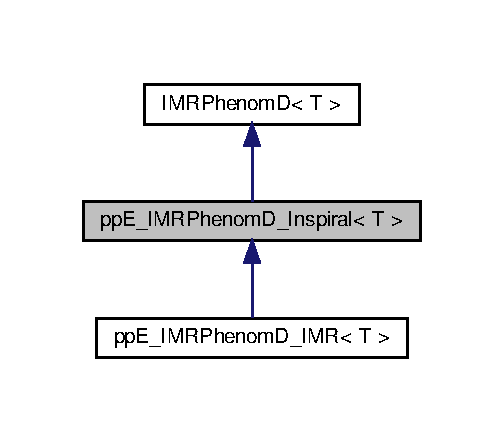
\includegraphics[width=350pt]{classppE__IMRPhenomD__Inspiral__inherit__graph}
\end{center}
\end{figure}


Collaboration diagram for pp\+E\+\_\+\+I\+M\+R\+Phenom\+D\+\_\+\+Inspiral$<$ T $>$\+:
\nopagebreak
\begin{figure}[H]
\begin{center}
\leavevmode
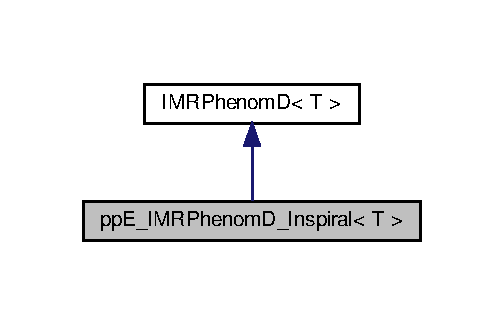
\includegraphics[width=242pt]{classppE__IMRPhenomD__Inspiral__coll__graph}
\end{center}
\end{figure}
\doxysubsection*{Public Member Functions}
\begin{DoxyCompactItemize}
\item 
\mbox{\Hypertarget{classppE__IMRPhenomD__Inspiral_a3187c9dba10e42f0bf20fb1e3bac9a52}\label{classppE__IMRPhenomD__Inspiral_a3187c9dba10e42f0bf20fb1e3bac9a52}} 
virtual T \mbox{\hyperlink{classppE__IMRPhenomD__Inspiral_a3187c9dba10e42f0bf20fb1e3bac9a52}{phase\+\_\+ins}} (T f, \mbox{\hyperlink{structsource__parameters}{source\+\_\+parameters}}$<$ T $>$ $\ast$param, T $\ast$pn\+\_\+coeff, \mbox{\hyperlink{structlambda__parameters}{lambda\+\_\+parameters}}$<$ T $>$ $\ast$lambda, \mbox{\hyperlink{structuseful__powers}{useful\+\_\+powers}}$<$ T $>$ $\ast$pow)
\begin{DoxyCompactList}\small\item\em Overloaded method for the inspiral portion of the phase. \end{DoxyCompactList}\item 
virtual T \mbox{\hyperlink{classppE__IMRPhenomD__Inspiral_ae297c077497d34a2632c55a7dafb9e83}{Dphase\+\_\+ins}} (T f, \mbox{\hyperlink{structsource__parameters}{source\+\_\+parameters}}$<$ T $>$ $\ast$param, T $\ast$pn\+\_\+coeff, \mbox{\hyperlink{structlambda__parameters}{lambda\+\_\+parameters}}$<$ T $>$ $\ast$lambda)
\begin{DoxyCompactList}\small\item\em Calculates the derivative of the inspiral phase for frequency f. \end{DoxyCompactList}\item 
\mbox{\Hypertarget{classppE__IMRPhenomD__Inspiral_ab6fe831f7c11840235dac2433ba14f82}\label{classppE__IMRPhenomD__Inspiral_ab6fe831f7c11840235dac2433ba14f82}} 
virtual void {\bfseries fisher\+\_\+calculation\+\_\+sky\+\_\+averaged} (double $\ast$frequency, int length, \mbox{\hyperlink{classgen__params}{gen\+\_\+params}} $\ast$parameters, double $\ast$$\ast$amplitude\+\_\+deriv, double $\ast$$\ast$phase\+\_\+deriv, double $\ast$amplitude, int $\ast$amp\+\_\+tapes, int $\ast$phase\+\_\+tapes)
\item 
virtual void \mbox{\hyperlink{classppE__IMRPhenomD__Inspiral_a87474cac9d6086d5625f79e28970b5ed}{amplitude\+\_\+tape}} (\mbox{\hyperlink{structsource__parameters}{source\+\_\+parameters}}$<$ double $>$ $\ast$input\+\_\+params, int $\ast$tape)
\begin{DoxyCompactList}\small\item\em Creates the tapes for derivatives of the amplitude. \end{DoxyCompactList}\item 
virtual void \mbox{\hyperlink{classppE__IMRPhenomD__Inspiral_a2fb1a8fb66e4204dbe397b792933afbe}{phase\+\_\+tape}} (\mbox{\hyperlink{structsource__parameters}{source\+\_\+parameters}}$<$ double $>$ $\ast$input\+\_\+params, int $\ast$tape)
\begin{DoxyCompactList}\small\item\em Creates the tapes for derivatives of phase. \end{DoxyCompactList}\item 
virtual void \mbox{\hyperlink{classppE__IMRPhenomD__Inspiral_a97d35197595f31d6cfbf6a8cf7c9a9ad}{construct\+\_\+amplitude\+\_\+derivative}} (double $\ast$frequencies, int length, int dimension, double $\ast$$\ast$amplitude\+\_\+derivative, \mbox{\hyperlink{structsource__parameters}{source\+\_\+parameters}}$<$ double $>$ $\ast$input\+\_\+params, int $\ast$tapes=N\+U\+LL)
\begin{DoxyCompactList}\small\item\em Construct the derivative of the amplitude for a given source evaluated by the given frequency. \end{DoxyCompactList}\item 
virtual void \mbox{\hyperlink{classppE__IMRPhenomD__Inspiral_a28d189808db2bd204e0d0051a1ed6427}{construct\+\_\+phase\+\_\+derivative}} (double $\ast$frequencies, int length, int dimension, double $\ast$$\ast$phase\+\_\+derivative, \mbox{\hyperlink{structsource__parameters}{source\+\_\+parameters}}$<$ double $>$ $\ast$input\+\_\+params, int $\ast$tapes=N\+U\+LL)
\begin{DoxyCompactList}\small\item\em Construct the derivative of the phase for a given source evaluated by the given frequency. \end{DoxyCompactList}\end{DoxyCompactItemize}


\doxysubsection{Detailed Description}
\subsubsection*{template$<$class T$>$\newline
class pp\+E\+\_\+\+I\+M\+R\+Phenom\+D\+\_\+\+Inspiral$<$ T $>$}

Class that extends the \mbox{\hyperlink{classIMRPhenomD}{I\+M\+R\+PhenomD}} waveform to include non-\/\+GR terms in the inspiral portion of the phase. This is an appropriate waveform choice for generation effects, but not necessarily for propagation effects 

\doxysubsection{Member Function Documentation}
\mbox{\Hypertarget{classppE__IMRPhenomD__Inspiral_a87474cac9d6086d5625f79e28970b5ed}\label{classppE__IMRPhenomD__Inspiral_a87474cac9d6086d5625f79e28970b5ed}} 
\index{ppE\_IMRPhenomD\_Inspiral$<$ T $>$@{ppE\_IMRPhenomD\_Inspiral$<$ T $>$}!amplitude\_tape@{amplitude\_tape}}
\index{amplitude\_tape@{amplitude\_tape}!ppE\_IMRPhenomD\_Inspiral$<$ T $>$@{ppE\_IMRPhenomD\_Inspiral$<$ T $>$}}
\doxysubsubsection{\texorpdfstring{amplitude\_tape()}{amplitude\_tape()}}
{\footnotesize\ttfamily template$<$class T $>$ \\
void \mbox{\hyperlink{classppE__IMRPhenomD__Inspiral}{pp\+E\+\_\+\+I\+M\+R\+Phenom\+D\+\_\+\+Inspiral}}$<$ T $>$\+::amplitude\+\_\+tape (\begin{DoxyParamCaption}\item[{\mbox{\hyperlink{structsource__parameters}{source\+\_\+parameters}}$<$ double $>$ $\ast$}]{input\+\_\+params,  }\item[{int $\ast$}]{tape }\end{DoxyParamCaption})\hspace{0.3cm}{\ttfamily [virtual]}}



Creates the tapes for derivatives of the amplitude. 

For efficiency in long runs of large sets of fishers, the tapes can be precomputed and reused 
\begin{DoxyParams}{Parameters}
{\em input\+\_\+params} & source parameters structure of the desired source \\
\hline
{\em tape} & tape ids \\
\hline
\end{DoxyParams}


Reimplemented from \mbox{\hyperlink{classIMRPhenomD_a6fbe3c51ee3eb66d332dc87a9fdf5bd4}{I\+M\+R\+Phenom\+D$<$ T $>$}}.



Reimplemented in \mbox{\hyperlink{classppE__IMRPhenomD__IMR_a3119a07c11ed53ae94823b11c5234c4f}{pp\+E\+\_\+\+I\+M\+R\+Phenom\+D\+\_\+\+I\+M\+R$<$ T $>$}}.

\mbox{\Hypertarget{classppE__IMRPhenomD__Inspiral_a97d35197595f31d6cfbf6a8cf7c9a9ad}\label{classppE__IMRPhenomD__Inspiral_a97d35197595f31d6cfbf6a8cf7c9a9ad}} 
\index{ppE\_IMRPhenomD\_Inspiral$<$ T $>$@{ppE\_IMRPhenomD\_Inspiral$<$ T $>$}!construct\_amplitude\_derivative@{construct\_amplitude\_derivative}}
\index{construct\_amplitude\_derivative@{construct\_amplitude\_derivative}!ppE\_IMRPhenomD\_Inspiral$<$ T $>$@{ppE\_IMRPhenomD\_Inspiral$<$ T $>$}}
\doxysubsubsection{\texorpdfstring{construct\_amplitude\_derivative()}{construct\_amplitude\_derivative()}}
{\footnotesize\ttfamily template$<$class T $>$ \\
void \mbox{\hyperlink{classppE__IMRPhenomD__Inspiral}{pp\+E\+\_\+\+I\+M\+R\+Phenom\+D\+\_\+\+Inspiral}}$<$ T $>$\+::construct\+\_\+amplitude\+\_\+derivative (\begin{DoxyParamCaption}\item[{double $\ast$}]{frequencies,  }\item[{int}]{length,  }\item[{int}]{dimension,  }\item[{double $\ast$$\ast$}]{amplitude\+\_\+derivative,  }\item[{\mbox{\hyperlink{structsource__parameters}{source\+\_\+parameters}}$<$ double $>$ $\ast$}]{input\+\_\+params,  }\item[{int $\ast$}]{tapes = {\ttfamily NULL} }\end{DoxyParamCaption})\hspace{0.3cm}{\ttfamily [virtual]}}



Construct the derivative of the amplitude for a given source evaluated by the given frequency. 

Order of output\+: dh/d \textbackslash{}theta \+: \textbackslash{}theta \textbackslash{}el \{A0,tc, phic, chirp mass, eta, symmetric spin, antisymmetric spin\} 
\begin{DoxyParams}{Parameters}
{\em frequencies} & input array of frequency \\
\hline
{\em length} & length of the frequency array \\
\hline
{\em amplitude\+\_\+derivative} & $<$ dimension of the fisher output array for all the derivatives double\mbox{[}dimension\mbox{]}\mbox{[}length\mbox{]} \\
\hline
{\em input\+\_\+params} & Source parameters structure for the source \\
\hline
{\em tapes} & int array of tape ids, if N\+U\+LL, these will be calculated \\
\hline
\end{DoxyParams}


Reimplemented from \mbox{\hyperlink{classIMRPhenomD_a4142331cc7a6471d13274b1ac8727378}{I\+M\+R\+Phenom\+D$<$ T $>$}}.



Reimplemented in \mbox{\hyperlink{classppE__IMRPhenomD__IMR_a5b80e5ae4dd83da49beb15e6e5f17715}{pp\+E\+\_\+\+I\+M\+R\+Phenom\+D\+\_\+\+I\+M\+R$<$ T $>$}}.

\mbox{\Hypertarget{classppE__IMRPhenomD__Inspiral_a28d189808db2bd204e0d0051a1ed6427}\label{classppE__IMRPhenomD__Inspiral_a28d189808db2bd204e0d0051a1ed6427}} 
\index{ppE\_IMRPhenomD\_Inspiral$<$ T $>$@{ppE\_IMRPhenomD\_Inspiral$<$ T $>$}!construct\_phase\_derivative@{construct\_phase\_derivative}}
\index{construct\_phase\_derivative@{construct\_phase\_derivative}!ppE\_IMRPhenomD\_Inspiral$<$ T $>$@{ppE\_IMRPhenomD\_Inspiral$<$ T $>$}}
\doxysubsubsection{\texorpdfstring{construct\_phase\_derivative()}{construct\_phase\_derivative()}}
{\footnotesize\ttfamily template$<$class T $>$ \\
void \mbox{\hyperlink{classppE__IMRPhenomD__Inspiral}{pp\+E\+\_\+\+I\+M\+R\+Phenom\+D\+\_\+\+Inspiral}}$<$ T $>$\+::construct\+\_\+phase\+\_\+derivative (\begin{DoxyParamCaption}\item[{double $\ast$}]{frequencies,  }\item[{int}]{length,  }\item[{int}]{dimension,  }\item[{double $\ast$$\ast$}]{phase\+\_\+derivative,  }\item[{\mbox{\hyperlink{structsource__parameters}{source\+\_\+parameters}}$<$ double $>$ $\ast$}]{input\+\_\+params,  }\item[{int $\ast$}]{tapes = {\ttfamily NULL} }\end{DoxyParamCaption})\hspace{0.3cm}{\ttfamily [virtual]}}



Construct the derivative of the phase for a given source evaluated by the given frequency. 

Order of output\+: dh/d \textbackslash{}theta \+: \textbackslash{}theta \textbackslash{}el \{A0,tc, phic, chirp mass, eta, symmetric spin, antisymmetric spin\} 
\begin{DoxyParams}{Parameters}
{\em frequencies} & input array of frequency \\
\hline
{\em length} & length of the frequency array \\
\hline
{\em phase\+\_\+derivative} & $<$ dimension of the fisher output array for all the derivatives double\mbox{[}dimension\mbox{]}\mbox{[}length\mbox{]} \\
\hline
{\em input\+\_\+params} & Source parameters structure for the source \\
\hline
{\em tapes} & int array of tape ids, if N\+U\+LL, these will be calculated \\
\hline
\end{DoxyParams}


Reimplemented from \mbox{\hyperlink{classIMRPhenomD_a26da276caf4c148016f558541d6914f6}{I\+M\+R\+Phenom\+D$<$ T $>$}}.



Reimplemented in \mbox{\hyperlink{classppE__IMRPhenomD__IMR_a78151d1f34693b69cf6ccbc28df4caa6}{pp\+E\+\_\+\+I\+M\+R\+Phenom\+D\+\_\+\+I\+M\+R$<$ T $>$}}.

\mbox{\Hypertarget{classppE__IMRPhenomD__Inspiral_ae297c077497d34a2632c55a7dafb9e83}\label{classppE__IMRPhenomD__Inspiral_ae297c077497d34a2632c55a7dafb9e83}} 
\index{ppE\_IMRPhenomD\_Inspiral$<$ T $>$@{ppE\_IMRPhenomD\_Inspiral$<$ T $>$}!Dphase\_ins@{Dphase\_ins}}
\index{Dphase\_ins@{Dphase\_ins}!ppE\_IMRPhenomD\_Inspiral$<$ T $>$@{ppE\_IMRPhenomD\_Inspiral$<$ T $>$}}
\doxysubsubsection{\texorpdfstring{Dphase\_ins()}{Dphase\_ins()}}
{\footnotesize\ttfamily template$<$class T $>$ \\
T \mbox{\hyperlink{classppE__IMRPhenomD__Inspiral}{pp\+E\+\_\+\+I\+M\+R\+Phenom\+D\+\_\+\+Inspiral}}$<$ T $>$\+::Dphase\+\_\+ins (\begin{DoxyParamCaption}\item[{T}]{f,  }\item[{\mbox{\hyperlink{structsource__parameters}{source\+\_\+parameters}}$<$ T $>$ $\ast$}]{param,  }\item[{T $\ast$}]{pn\+\_\+coeff,  }\item[{\mbox{\hyperlink{structlambda__parameters}{lambda\+\_\+parameters}}$<$ T $>$ $\ast$}]{lambda }\end{DoxyParamCaption})\hspace{0.3cm}{\ttfamily [virtual]}}



Calculates the derivative of the inspiral phase for frequency f. 

For phase continuity and smoothness return a T 

Reimplemented from \mbox{\hyperlink{classIMRPhenomD_ab840b052576cde8a9e802c5784d24092}{I\+M\+R\+Phenom\+D$<$ T $>$}}.

\mbox{\Hypertarget{classppE__IMRPhenomD__Inspiral_a2fb1a8fb66e4204dbe397b792933afbe}\label{classppE__IMRPhenomD__Inspiral_a2fb1a8fb66e4204dbe397b792933afbe}} 
\index{ppE\_IMRPhenomD\_Inspiral$<$ T $>$@{ppE\_IMRPhenomD\_Inspiral$<$ T $>$}!phase\_tape@{phase\_tape}}
\index{phase\_tape@{phase\_tape}!ppE\_IMRPhenomD\_Inspiral$<$ T $>$@{ppE\_IMRPhenomD\_Inspiral$<$ T $>$}}
\doxysubsubsection{\texorpdfstring{phase\_tape()}{phase\_tape()}}
{\footnotesize\ttfamily template$<$class T $>$ \\
void \mbox{\hyperlink{classppE__IMRPhenomD__Inspiral}{pp\+E\+\_\+\+I\+M\+R\+Phenom\+D\+\_\+\+Inspiral}}$<$ T $>$\+::phase\+\_\+tape (\begin{DoxyParamCaption}\item[{\mbox{\hyperlink{structsource__parameters}{source\+\_\+parameters}}$<$ double $>$ $\ast$}]{input\+\_\+params,  }\item[{int $\ast$}]{tape }\end{DoxyParamCaption})\hspace{0.3cm}{\ttfamily [virtual]}}



Creates the tapes for derivatives of phase. 

For efficiency in long runs of large sets of fishers, the tapes can be precomputed and reused 
\begin{DoxyParams}{Parameters}
{\em input\+\_\+params} & source parameters structure of the desired source \\
\hline
{\em tape} & tape ids \\
\hline
\end{DoxyParams}


Reimplemented from \mbox{\hyperlink{classIMRPhenomD_ae456c25f87c34487e6e05f9cf5d2d08c}{I\+M\+R\+Phenom\+D$<$ T $>$}}.



Reimplemented in \mbox{\hyperlink{classppE__IMRPhenomD__IMR_acf2ed8617b3e24ecc273a409ff579ce4}{pp\+E\+\_\+\+I\+M\+R\+Phenom\+D\+\_\+\+I\+M\+R$<$ T $>$}}.



The documentation for this class was generated from the following files\+:\begin{DoxyCompactItemize}
\item 
include/gwat/\mbox{\hyperlink{ppE__IMRPhenomD_8h}{pp\+E\+\_\+\+I\+M\+R\+Phenom\+D.\+h}}\item 
src/\mbox{\hyperlink{ppE__IMRPhenomD_8cpp}{pp\+E\+\_\+\+I\+M\+R\+Phenom\+D.\+cpp}}\end{DoxyCompactItemize}

\hypertarget{classppE__IMRPhenomPv2__IMR}{}\section{pp\+E\+\_\+\+I\+M\+R\+Phenom\+Pv2\+\_\+\+I\+MR$<$ T $>$ Class Template Reference}
\label{classppE__IMRPhenomPv2__IMR}\index{pp\+E\+\_\+\+I\+M\+R\+Phenom\+Pv2\+\_\+\+I\+M\+R$<$ T $>$@{pp\+E\+\_\+\+I\+M\+R\+Phenom\+Pv2\+\_\+\+I\+M\+R$<$ T $>$}}


Inheritance diagram for pp\+E\+\_\+\+I\+M\+R\+Phenom\+Pv2\+\_\+\+I\+MR$<$ T $>$\+:\nopagebreak
\begin{figure}[H]
\begin{center}
\leavevmode
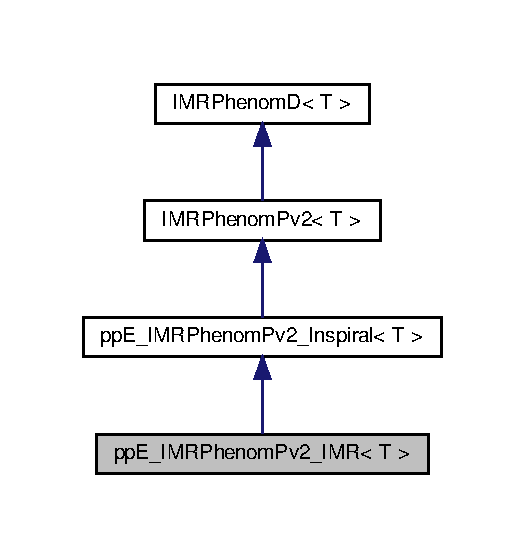
\includegraphics[width=252pt]{classppE__IMRPhenomPv2__IMR__inherit__graph}
\end{center}
\end{figure}


Collaboration diagram for pp\+E\+\_\+\+I\+M\+R\+Phenom\+Pv2\+\_\+\+I\+MR$<$ T $>$\+:\nopagebreak
\begin{figure}[H]
\begin{center}
\leavevmode
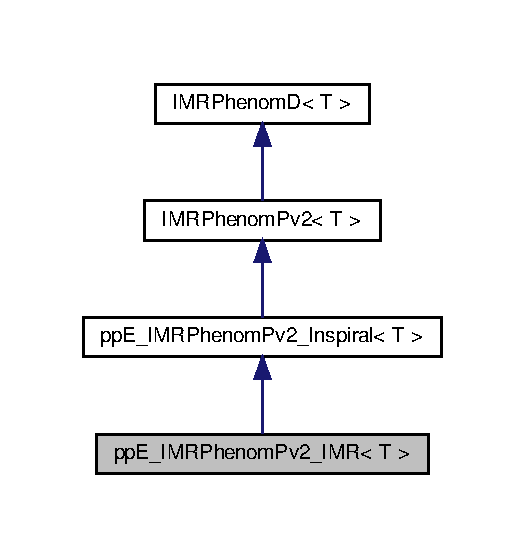
\includegraphics[width=252pt]{classppE__IMRPhenomPv2__IMR__coll__graph}
\end{center}
\end{figure}
\subsection*{Public Member Functions}
\begin{DoxyCompactItemize}
\item 
virtual T \hyperlink{classppE__IMRPhenomPv2__IMR_a498e1d8b7ea85028b295feb9487ca066}{phase\+\_\+mr} (T f, \hyperlink{structsource__parameters}{source\+\_\+parameters}$<$ T $>$ $\ast$param, \hyperlink{structlambda__parameters}{lambda\+\_\+parameters}$<$ T $>$ $\ast$lambda)
\item 
virtual T \hyperlink{classppE__IMRPhenomPv2__IMR_acaccc873b9eab76c4640c478e69a7e20}{Dphase\+\_\+mr} (T f, \hyperlink{structsource__parameters}{source\+\_\+parameters}$<$ T $>$ $\ast$param, \hyperlink{structlambda__parameters}{lambda\+\_\+parameters}$<$ T $>$ $\ast$lambda)
\begin{DoxyCompactList}\small\item\em Calculates the derivative of the merger-\/ringdown phase for frequency f. \end{DoxyCompactList}\item 
virtual T \hyperlink{classppE__IMRPhenomPv2__IMR_a713b095dacec9472b5361c1caf884347}{phase\+\_\+int} (T f, \hyperlink{structsource__parameters}{source\+\_\+parameters}$<$ T $>$ $\ast$param, \hyperlink{structlambda__parameters}{lambda\+\_\+parameters}$<$ T $>$ $\ast$lambda)
\begin{DoxyCompactList}\small\item\em Calculates the intermediate phase for frequency f. \end{DoxyCompactList}\item 
virtual T \hyperlink{classppE__IMRPhenomPv2__IMR_af192ae33e9293ed487b583d21f6c5bcd}{Dphase\+\_\+int} (T f, \hyperlink{structsource__parameters}{source\+\_\+parameters}$<$ T $>$ $\ast$param, \hyperlink{structlambda__parameters}{lambda\+\_\+parameters}$<$ T $>$ $\ast$lambda)
\begin{DoxyCompactList}\small\item\em Calculates the derivative of the intermediate phase for frequency f. \end{DoxyCompactList}\end{DoxyCompactItemize}


\subsection{Member Function Documentation}
\mbox{\Hypertarget{classppE__IMRPhenomPv2__IMR_af192ae33e9293ed487b583d21f6c5bcd}\label{classppE__IMRPhenomPv2__IMR_af192ae33e9293ed487b583d21f6c5bcd}} 
\index{pp\+E\+\_\+\+I\+M\+R\+Phenom\+Pv2\+\_\+\+I\+MR@{pp\+E\+\_\+\+I\+M\+R\+Phenom\+Pv2\+\_\+\+I\+MR}!Dphase\+\_\+int@{Dphase\+\_\+int}}
\index{Dphase\+\_\+int@{Dphase\+\_\+int}!pp\+E\+\_\+\+I\+M\+R\+Phenom\+Pv2\+\_\+\+I\+MR@{pp\+E\+\_\+\+I\+M\+R\+Phenom\+Pv2\+\_\+\+I\+MR}}
\subsubsection{\texorpdfstring{Dphase\+\_\+int()}{Dphase\_int()}}
{\footnotesize\ttfamily template$<$class T $>$ \\
T \hyperlink{classppE__IMRPhenomPv2__IMR}{pp\+E\+\_\+\+I\+M\+R\+Phenom\+Pv2\+\_\+\+I\+MR}$<$ T $>$\+::Dphase\+\_\+int (\begin{DoxyParamCaption}\item[{T}]{f,  }\item[{\hyperlink{structsource__parameters}{source\+\_\+parameters}$<$ T $>$ $\ast$}]{param,  }\item[{\hyperlink{structlambda__parameters}{lambda\+\_\+parameters}$<$ T $>$ $\ast$}]{lambda }\end{DoxyParamCaption})\hspace{0.3cm}{\ttfamily [virtual]}}



Calculates the derivative of the intermediate phase for frequency f. 

For phase continuity and smoothness return a T 

Reimplemented from \hyperlink{classIMRPhenomD_a8d395e33bd420cdc996a6487302af36a}{I\+M\+R\+Phenom\+D$<$ T $>$}.

\mbox{\Hypertarget{classppE__IMRPhenomPv2__IMR_acaccc873b9eab76c4640c478e69a7e20}\label{classppE__IMRPhenomPv2__IMR_acaccc873b9eab76c4640c478e69a7e20}} 
\index{pp\+E\+\_\+\+I\+M\+R\+Phenom\+Pv2\+\_\+\+I\+MR@{pp\+E\+\_\+\+I\+M\+R\+Phenom\+Pv2\+\_\+\+I\+MR}!Dphase\+\_\+mr@{Dphase\+\_\+mr}}
\index{Dphase\+\_\+mr@{Dphase\+\_\+mr}!pp\+E\+\_\+\+I\+M\+R\+Phenom\+Pv2\+\_\+\+I\+MR@{pp\+E\+\_\+\+I\+M\+R\+Phenom\+Pv2\+\_\+\+I\+MR}}
\subsubsection{\texorpdfstring{Dphase\+\_\+mr()}{Dphase\_mr()}}
{\footnotesize\ttfamily template$<$class T $>$ \\
T \hyperlink{classppE__IMRPhenomPv2__IMR}{pp\+E\+\_\+\+I\+M\+R\+Phenom\+Pv2\+\_\+\+I\+MR}$<$ T $>$\+::Dphase\+\_\+mr (\begin{DoxyParamCaption}\item[{T}]{f,  }\item[{\hyperlink{structsource__parameters}{source\+\_\+parameters}$<$ T $>$ $\ast$}]{param,  }\item[{\hyperlink{structlambda__parameters}{lambda\+\_\+parameters}$<$ T $>$ $\ast$}]{lambda }\end{DoxyParamCaption})\hspace{0.3cm}{\ttfamily [virtual]}}



Calculates the derivative of the merger-\/ringdown phase for frequency f. 

For phase continuity and smoothness return a T 

Reimplemented from \hyperlink{classIMRPhenomD_ab4a74828eacee645bac43b0af2c510e1}{I\+M\+R\+Phenom\+D$<$ T $>$}.

\mbox{\Hypertarget{classppE__IMRPhenomPv2__IMR_a713b095dacec9472b5361c1caf884347}\label{classppE__IMRPhenomPv2__IMR_a713b095dacec9472b5361c1caf884347}} 
\index{pp\+E\+\_\+\+I\+M\+R\+Phenom\+Pv2\+\_\+\+I\+MR@{pp\+E\+\_\+\+I\+M\+R\+Phenom\+Pv2\+\_\+\+I\+MR}!phase\+\_\+int@{phase\+\_\+int}}
\index{phase\+\_\+int@{phase\+\_\+int}!pp\+E\+\_\+\+I\+M\+R\+Phenom\+Pv2\+\_\+\+I\+MR@{pp\+E\+\_\+\+I\+M\+R\+Phenom\+Pv2\+\_\+\+I\+MR}}
\subsubsection{\texorpdfstring{phase\+\_\+int()}{phase\_int()}}
{\footnotesize\ttfamily template$<$class T $>$ \\
T \hyperlink{classppE__IMRPhenomPv2__IMR}{pp\+E\+\_\+\+I\+M\+R\+Phenom\+Pv2\+\_\+\+I\+MR}$<$ T $>$\+::phase\+\_\+int (\begin{DoxyParamCaption}\item[{T}]{f,  }\item[{\hyperlink{structsource__parameters}{source\+\_\+parameters}$<$ T $>$ $\ast$}]{param,  }\item[{\hyperlink{structlambda__parameters}{lambda\+\_\+parameters}$<$ T $>$ $\ast$}]{lambda }\end{DoxyParamCaption})\hspace{0.3cm}{\ttfamily [virtual]}}



Calculates the intermediate phase for frequency f. 

return a T 

Reimplemented from \hyperlink{classIMRPhenomD_ad6a8bb9539e7494cad8a91aaa950cf50}{I\+M\+R\+Phenom\+D$<$ T $>$}.

\mbox{\Hypertarget{classppE__IMRPhenomPv2__IMR_a498e1d8b7ea85028b295feb9487ca066}\label{classppE__IMRPhenomPv2__IMR_a498e1d8b7ea85028b295feb9487ca066}} 
\index{pp\+E\+\_\+\+I\+M\+R\+Phenom\+Pv2\+\_\+\+I\+MR@{pp\+E\+\_\+\+I\+M\+R\+Phenom\+Pv2\+\_\+\+I\+MR}!phase\+\_\+mr@{phase\+\_\+mr}}
\index{phase\+\_\+mr@{phase\+\_\+mr}!pp\+E\+\_\+\+I\+M\+R\+Phenom\+Pv2\+\_\+\+I\+MR@{pp\+E\+\_\+\+I\+M\+R\+Phenom\+Pv2\+\_\+\+I\+MR}}
\subsubsection{\texorpdfstring{phase\+\_\+mr()}{phase\_mr()}}
{\footnotesize\ttfamily template$<$class T $>$ \\
T \hyperlink{classppE__IMRPhenomPv2__IMR}{pp\+E\+\_\+\+I\+M\+R\+Phenom\+Pv2\+\_\+\+I\+MR}$<$ T $>$\+::phase\+\_\+mr (\begin{DoxyParamCaption}\item[{T}]{f,  }\item[{\hyperlink{structsource__parameters}{source\+\_\+parameters}$<$ T $>$ $\ast$}]{param,  }\item[{\hyperlink{structlambda__parameters}{lambda\+\_\+parameters}$<$ T $>$ $\ast$}]{lambda }\end{DoxyParamCaption})\hspace{0.3cm}{\ttfamily [virtual]}}

/\+Brief Parameter transformtion to precalculate needed parameters for PhenomP from source parameters

Pretty much stolen verbatim from lalsuite 

Reimplemented from \hyperlink{classIMRPhenomD_a2c9c226afc991458872e36bba204f395}{I\+M\+R\+Phenom\+D$<$ T $>$}.



The documentation for this class was generated from the following files\+:\begin{DoxyCompactItemize}
\item 
include/gwat/\hyperlink{ppE__IMRPhenomP_8h}{pp\+E\+\_\+\+I\+M\+R\+Phenom\+P.\+h}\item 
src/\hyperlink{ppE__IMRPhenomP_8cpp}{pp\+E\+\_\+\+I\+M\+R\+Phenom\+P.\+cpp}\end{DoxyCompactItemize}

\hypertarget{classppE__IMRPhenomPv2__Inspiral}{}\doxysection{pp\+E\+\_\+\+I\+M\+R\+Phenom\+Pv2\+\_\+\+Inspiral$<$ T $>$ Class Template Reference}
\label{classppE__IMRPhenomPv2__Inspiral}\index{ppE\_IMRPhenomPv2\_Inspiral$<$ T $>$@{ppE\_IMRPhenomPv2\_Inspiral$<$ T $>$}}


Inheritance diagram for pp\+E\+\_\+\+I\+M\+R\+Phenom\+Pv2\+\_\+\+Inspiral$<$ T $>$\+:
\nopagebreak
\begin{figure}[H]
\begin{center}
\leavevmode
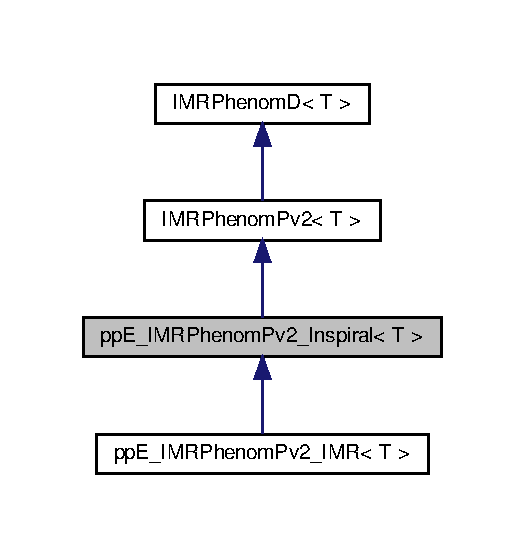
\includegraphics[width=252pt]{classppE__IMRPhenomPv2__Inspiral__inherit__graph}
\end{center}
\end{figure}


Collaboration diagram for pp\+E\+\_\+\+I\+M\+R\+Phenom\+Pv2\+\_\+\+Inspiral$<$ T $>$\+:
\nopagebreak
\begin{figure}[H]
\begin{center}
\leavevmode
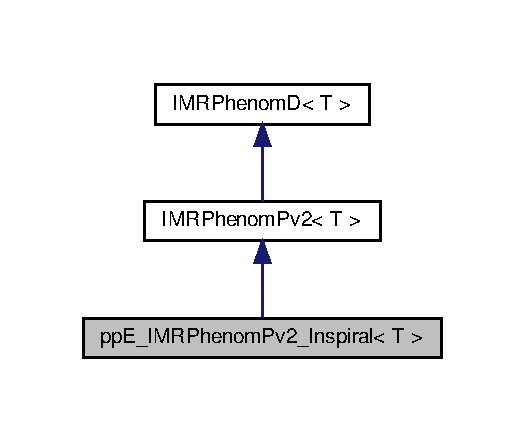
\includegraphics[width=252pt]{classppE__IMRPhenomPv2__Inspiral__coll__graph}
\end{center}
\end{figure}
\doxysubsection*{Public Member Functions}
\begin{DoxyCompactItemize}
\item 
virtual T \mbox{\hyperlink{classppE__IMRPhenomPv2__Inspiral_a829118c33d81ed4bcc4b48e7349c58f6}{phase\+\_\+ins}} (T f, \mbox{\hyperlink{structsource__parameters}{source\+\_\+parameters}}$<$ T $>$ $\ast$param, T $\ast$pn\+\_\+coeff, \mbox{\hyperlink{structlambda__parameters}{lambda\+\_\+parameters}}$<$ T $>$ $\ast$lambda, \mbox{\hyperlink{structuseful__powers}{useful\+\_\+powers}}$<$ T $>$ $\ast$pow)
\begin{DoxyCompactList}\small\item\em Calculates the inspiral phase for frequency f with precomputed powers of MF and PI for speed. \end{DoxyCompactList}\item 
virtual T \mbox{\hyperlink{classppE__IMRPhenomPv2__Inspiral_a2975dbfd6aba25f57b93dfb68fac24b8}{Dphase\+\_\+ins}} (T f, \mbox{\hyperlink{structsource__parameters}{source\+\_\+parameters}}$<$ T $>$ $\ast$param, T $\ast$pn\+\_\+coeff, \mbox{\hyperlink{structlambda__parameters}{lambda\+\_\+parameters}}$<$ T $>$ $\ast$lambda)
\begin{DoxyCompactList}\small\item\em Calculates the derivative of the inspiral phase for frequency f. \end{DoxyCompactList}\end{DoxyCompactItemize}


\doxysubsection{Member Function Documentation}
\mbox{\Hypertarget{classppE__IMRPhenomPv2__Inspiral_a2975dbfd6aba25f57b93dfb68fac24b8}\label{classppE__IMRPhenomPv2__Inspiral_a2975dbfd6aba25f57b93dfb68fac24b8}} 
\index{ppE\_IMRPhenomPv2\_Inspiral$<$ T $>$@{ppE\_IMRPhenomPv2\_Inspiral$<$ T $>$}!Dphase\_ins@{Dphase\_ins}}
\index{Dphase\_ins@{Dphase\_ins}!ppE\_IMRPhenomPv2\_Inspiral$<$ T $>$@{ppE\_IMRPhenomPv2\_Inspiral$<$ T $>$}}
\doxysubsubsection{\texorpdfstring{Dphase\_ins()}{Dphase\_ins()}}
{\footnotesize\ttfamily template$<$class T $>$ \\
T \mbox{\hyperlink{classppE__IMRPhenomPv2__Inspiral}{pp\+E\+\_\+\+I\+M\+R\+Phenom\+Pv2\+\_\+\+Inspiral}}$<$ T $>$\+::Dphase\+\_\+ins (\begin{DoxyParamCaption}\item[{T}]{f,  }\item[{\mbox{\hyperlink{structsource__parameters}{source\+\_\+parameters}}$<$ T $>$ $\ast$}]{param,  }\item[{T $\ast$}]{pn\+\_\+coeff,  }\item[{\mbox{\hyperlink{structlambda__parameters}{lambda\+\_\+parameters}}$<$ T $>$ $\ast$}]{lambda }\end{DoxyParamCaption})\hspace{0.3cm}{\ttfamily [virtual]}}



Calculates the derivative of the inspiral phase for frequency f. 

For phase continuity and smoothness return a T 

Reimplemented from \mbox{\hyperlink{classIMRPhenomD_ab840b052576cde8a9e802c5784d24092}{I\+M\+R\+Phenom\+D$<$ T $>$}}.

\mbox{\Hypertarget{classppE__IMRPhenomPv2__Inspiral_a829118c33d81ed4bcc4b48e7349c58f6}\label{classppE__IMRPhenomPv2__Inspiral_a829118c33d81ed4bcc4b48e7349c58f6}} 
\index{ppE\_IMRPhenomPv2\_Inspiral$<$ T $>$@{ppE\_IMRPhenomPv2\_Inspiral$<$ T $>$}!phase\_ins@{phase\_ins}}
\index{phase\_ins@{phase\_ins}!ppE\_IMRPhenomPv2\_Inspiral$<$ T $>$@{ppE\_IMRPhenomPv2\_Inspiral$<$ T $>$}}
\doxysubsubsection{\texorpdfstring{phase\_ins()}{phase\_ins()}}
{\footnotesize\ttfamily template$<$class T $>$ \\
T \mbox{\hyperlink{classppE__IMRPhenomPv2__Inspiral}{pp\+E\+\_\+\+I\+M\+R\+Phenom\+Pv2\+\_\+\+Inspiral}}$<$ T $>$\+::phase\+\_\+ins (\begin{DoxyParamCaption}\item[{T}]{f,  }\item[{\mbox{\hyperlink{structsource__parameters}{source\+\_\+parameters}}$<$ T $>$ $\ast$}]{param,  }\item[{T $\ast$}]{pn\+\_\+coeff,  }\item[{\mbox{\hyperlink{structlambda__parameters}{lambda\+\_\+parameters}}$<$ T $>$ $\ast$}]{lambda,  }\item[{\mbox{\hyperlink{structuseful__powers}{useful\+\_\+powers}}$<$ T $>$ $\ast$}]{pow }\end{DoxyParamCaption})\hspace{0.3cm}{\ttfamily [virtual]}}



Calculates the inspiral phase for frequency f with precomputed powers of MF and PI for speed. 

return a T

extra argument of precomputed powers of MF and pi, contained in the structure useful\+\_\+powers$<$\+T$>$ 

Reimplemented from \mbox{\hyperlink{classIMRPhenomD_a7073ff2be22b0251ca419d0b69dd9990}{I\+M\+R\+Phenom\+D$<$ T $>$}}.



The documentation for this class was generated from the following files\+:\begin{DoxyCompactItemize}
\item 
include/gwat/\mbox{\hyperlink{ppE__IMRPhenomP_8h}{pp\+E\+\_\+\+I\+M\+R\+Phenom\+P.\+h}}\item 
src/\mbox{\hyperlink{ppE__IMRPhenomP_8cpp}{pp\+E\+\_\+\+I\+M\+R\+Phenom\+P.\+cpp}}\end{DoxyCompactItemize}

\hypertarget{classsampler}{}\doxysection{sampler Class Reference}
\label{classsampler}\index{sampler@{sampler}}


{\ttfamily \#include $<$mcmc\+\_\+sampler\+\_\+internals.\+h$>$}

\doxysubsection*{Public Attributes}
\begin{DoxyCompactItemize}
\item 
\mbox{\Hypertarget{classsampler_a0a556351f7c28b8577e5e7f8106ae626}\label{classsampler_a0a556351f7c28b8577e5e7f8106ae626}} 
int {\bfseries types\+\_\+of\+\_\+steps} = 5
\item 
\mbox{\Hypertarget{classsampler_a5970eec37aea2dc10223ef31668bc2c8}\label{classsampler_a5970eec37aea2dc10223ef31668bc2c8}} 
double $\ast$$\ast$ {\bfseries step\+\_\+prob}
\item 
\mbox{\Hypertarget{classsampler_adc62297d359d487fc09358b69df3baba}\label{classsampler_adc62297d359d487fc09358b69df3baba}} 
double $\ast$$\ast$ {\bfseries prob\+\_\+boundaries}
\item 
\mbox{\Hypertarget{classsampler_aeab13d23abfd6582959f82201306bbd9}\label{classsampler_aeab13d23abfd6582959f82201306bbd9}} 
double $\ast$ {\bfseries chain\+\_\+temps}
\item 
\mbox{\Hypertarget{classsampler_a962e2016c8c5304d84731b34d603b221}\label{classsampler_a962e2016c8c5304d84731b34d603b221}} 
bool $\ast$ {\bfseries waiting}
\item 
\mbox{\Hypertarget{classsampler_a8d6b552c3e3f330fabdfdab1d214bb0c}\label{classsampler_a8d6b552c3e3f330fabdfdab1d214bb0c}} 
int $\ast$ {\bfseries chain\+\_\+pos}
\item 
\mbox{\Hypertarget{classsampler_af02dde10e178c15057266bd33783f9eb}\label{classsampler_af02dde10e178c15057266bd33783f9eb}} 
double {\bfseries swp\+\_\+freq}
\item 
\mbox{\Hypertarget{classsampler_a7ef923424ae51147137ed36e02e7ca29}\label{classsampler_a7ef923424ae51147137ed36e02e7ca29}} 
int {\bfseries chain\+\_\+N}
\item 
\mbox{\Hypertarget{classsampler_a67740d4b88501036e9f05955d4664708}\label{classsampler_a67740d4b88501036e9f05955d4664708}} 
int {\bfseries num\+Threads}
\item 
\mbox{\Hypertarget{classsampler_ad99bec294257a8e22b14091a403c5e41}\label{classsampler_ad99bec294257a8e22b14091a403c5e41}} 
int {\bfseries N\+\_\+steps}
\item 
\mbox{\Hypertarget{classsampler_aefce952ae3d54283ed05035cc7bb094d}\label{classsampler_aefce952ae3d54283ed05035cc7bb094d}} 
int {\bfseries dimension}
\item 
\mbox{\Hypertarget{classsampler_a26e43b6bc36c13a166bf6ae97bb2eac1}\label{classsampler_a26e43b6bc36c13a166bf6ae97bb2eac1}} 
int {\bfseries min\+\_\+dim}
\item 
\mbox{\Hypertarget{classsampler_ac377db38549868c3971029bcb071bb98}\label{classsampler_ac377db38549868c3971029bcb071bb98}} 
int {\bfseries max\+\_\+dim}
\item 
\mbox{\Hypertarget{classsampler_a6b85548a4adacf726b317954111aa681}\label{classsampler_a6b85548a4adacf726b317954111aa681}} 
bool {\bfseries fisher\+\_\+exist}
\item 
\mbox{\Hypertarget{classsampler_acd39963f4ab1bc2730c1dc13cfc1869e}\label{classsampler_acd39963f4ab1bc2730c1dc13cfc1869e}} 
bool $\ast$ {\bfseries de\+\_\+primed}
\item 
\mbox{\Hypertarget{classsampler_a94d70e8841cb2472895f5c275b70024f}\label{classsampler_a94d70e8841cb2472895f5c275b70024f}} 
int $\ast$ {\bfseries priority}
\item 
\mbox{\Hypertarget{classsampler_a6eb7e7801369e67ebc59bd1c97ce1c6c}\label{classsampler_a6eb7e7801369e67ebc59bd1c97ce1c6c}} 
bool $\ast$ {\bfseries ref\+\_\+chain\+\_\+status}
\item 
\mbox{\Hypertarget{classsampler_ac82b14511b477b6fb3f1031fd3eb8e6d}\label{classsampler_ac82b14511b477b6fb3f1031fd3eb8e6d}} 
bool {\bfseries prioritize\+\_\+cold\+\_\+chains} = false
\item 
\mbox{\Hypertarget{classsampler_aa751bde85363017a9cc66c5367c755d1}\label{classsampler_aa751bde85363017a9cc66c5367c755d1}} 
double $\ast$$\ast$$\ast$ {\bfseries output}
\item 
\mbox{\Hypertarget{classsampler_aa674666a7515ce0853734e1337ffd402}\label{classsampler_aa674666a7515ce0853734e1337ffd402}} 
bool {\bfseries pool}
\item 
\mbox{\Hypertarget{classsampler_af248578ba42f306ff0d9d1e47a75c055}\label{classsampler_af248578ba42f306ff0d9d1e47a75c055}} 
int {\bfseries progress} =0
\item 
\mbox{\Hypertarget{classsampler_a52a0fb22a7c5c9a1c875b0c09efc467b}\label{classsampler_a52a0fb22a7c5c9a1c875b0c09efc467b}} 
bool {\bfseries show\+\_\+progress}
\item 
\mbox{\Hypertarget{classsampler_a0d3c87df5d138ce4cd2286d55a54eb04}\label{classsampler_a0d3c87df5d138ce4cd2286d55a54eb04}} 
int {\bfseries num\+\_\+threads}
\item 
\mbox{\Hypertarget{classsampler_a19172e2dd561a1d2d77fb4557f8dfff1}\label{classsampler_a19172e2dd561a1d2d77fb4557f8dfff1}} 
int {\bfseries history\+\_\+length} =500
\item 
\mbox{\Hypertarget{classsampler_ae8c91af39ee6b6342becfb78b6bfc260}\label{classsampler_ae8c91af39ee6b6342becfb78b6bfc260}} 
int {\bfseries history\+\_\+update} =5
\item 
\mbox{\Hypertarget{classsampler_adfa5da34ec3c754245fbb4bef9b3c14d}\label{classsampler_adfa5da34ec3c754245fbb4bef9b3c14d}} 
int $\ast$ {\bfseries current\+\_\+hist\+\_\+pos}
\item 
\mbox{\Hypertarget{classsampler_aaf2d81b15fe8aae0a7a4c68074b70963}\label{classsampler_aaf2d81b15fe8aae0a7a4c68074b70963}} 
double $\ast$$\ast$$\ast$ {\bfseries history}
\item 
\mbox{\Hypertarget{classsampler_aa5de645803117a47d82015b1e76e7674}\label{classsampler_aa5de645803117a47d82015b1e76e7674}} 
int $\ast$$\ast$$\ast$ {\bfseries history\+\_\+status}
\item 
\mbox{\Hypertarget{classsampler_add57d174fcd91657e9acdddb6060905b}\label{classsampler_add57d174fcd91657e9acdddb6060905b}} 
double $\ast$ {\bfseries current\+\_\+likelihoods}
\item 
\mbox{\Hypertarget{classsampler_a54e672a5ebb85d55770f07581bffd945}\label{classsampler_a54e672a5ebb85d55770f07581bffd945}} 
int $\ast$ {\bfseries check\+\_\+stepsize\+\_\+freq}
\item 
\mbox{\Hypertarget{classsampler_a2ee866342b0fa6b36abf5e37de2200f7}\label{classsampler_a2ee866342b0fa6b36abf5e37de2200f7}} 
double $\ast$ {\bfseries max\+\_\+target\+\_\+accept\+\_\+ratio}
\item 
\mbox{\Hypertarget{classsampler_a8151e04ac80e69947f741daecd33bb0b}\label{classsampler_a8151e04ac80e69947f741daecd33bb0b}} 
double $\ast$ {\bfseries min\+\_\+target\+\_\+accept\+\_\+ratio}
\item 
\mbox{\Hypertarget{classsampler_ab2ca885ab273b052474c5c6a50101641}\label{classsampler_ab2ca885ab273b052474c5c6a50101641}} 
int $\ast$ {\bfseries gauss\+\_\+last\+\_\+accept\+\_\+ct}
\item 
\mbox{\Hypertarget{classsampler_ad27db60c348826ea2305b045dee2601b}\label{classsampler_ad27db60c348826ea2305b045dee2601b}} 
int $\ast$ {\bfseries gauss\+\_\+last\+\_\+reject\+\_\+ct}
\item 
\mbox{\Hypertarget{classsampler_a6326cc16d308d4d487df39bad968fb9a}\label{classsampler_a6326cc16d308d4d487df39bad968fb9a}} 
int $\ast$ {\bfseries de\+\_\+last\+\_\+accept\+\_\+ct}
\item 
\mbox{\Hypertarget{classsampler_afde1208f42942898d463f0b5c8eed880}\label{classsampler_afde1208f42942898d463f0b5c8eed880}} 
int $\ast$ {\bfseries de\+\_\+last\+\_\+reject\+\_\+ct}
\item 
\mbox{\Hypertarget{classsampler_ab2198c1496f90189a165aa4471bfdddd}\label{classsampler_ab2198c1496f90189a165aa4471bfdddd}} 
int $\ast$ {\bfseries fish\+\_\+last\+\_\+accept\+\_\+ct}
\item 
\mbox{\Hypertarget{classsampler_a9b2cbb8f29358160bbc16bbddb640e57}\label{classsampler_a9b2cbb8f29358160bbc16bbddb640e57}} 
int $\ast$ {\bfseries fish\+\_\+last\+\_\+reject\+\_\+ct}
\item 
\mbox{\Hypertarget{classsampler_a8682f3a38e907010a8a21a9a19207bc4}\label{classsampler_a8682f3a38e907010a8a21a9a19207bc4}} 
int $\ast$ {\bfseries R\+Jstep\+\_\+last\+\_\+accept\+\_\+ct}
\item 
\mbox{\Hypertarget{classsampler_a09859b32798ffd6cf39492bf89245cb4}\label{classsampler_a09859b32798ffd6cf39492bf89245cb4}} 
int $\ast$ {\bfseries R\+Jstep\+\_\+last\+\_\+reject\+\_\+ct}
\item 
\mbox{\Hypertarget{classsampler_acbbf9bdc68bd3089e06e4575813aaf1b}\label{classsampler_acbbf9bdc68bd3089e06e4575813aaf1b}} 
double $\ast$$\ast$ {\bfseries randgauss\+\_\+width}
\item 
\mbox{\Hypertarget{classsampler_afbaa3b490977775308c0fa26870a8486}\label{classsampler_afbaa3b490977775308c0fa26870a8486}} 
double $\ast$$\ast$$\ast$ {\bfseries fisher\+\_\+vecs}
\item 
\mbox{\Hypertarget{classsampler_a969aca461dc9adc844cd4f27b0896f47}\label{classsampler_a969aca461dc9adc844cd4f27b0896f47}} 
double $\ast$$\ast$ {\bfseries fisher\+\_\+vals}
\item 
\mbox{\Hypertarget{classsampler_aca7467144c29b5087a22b355a01ab6b1}\label{classsampler_aca7467144c29b5087a22b355a01ab6b1}} 
double $\ast$$\ast$$\ast$ {\bfseries fisher\+\_\+vecs\+\_\+prev}
\item 
\mbox{\Hypertarget{classsampler_a15cd44bab3ae8239b5d0160f0b57bf13}\label{classsampler_a15cd44bab3ae8239b5d0160f0b57bf13}} 
double $\ast$$\ast$ {\bfseries fisher\+\_\+vals\+\_\+prev}
\item 
\mbox{\Hypertarget{classsampler_ab1df1d497bc3246954239e3a329895eb}\label{classsampler_ab1df1d497bc3246954239e3a329895eb}} 
double $\ast$$\ast$$\ast$ {\bfseries fisher\+\_\+matrix}
\item 
\mbox{\Hypertarget{classsampler_a9776e8d0eb832b5349646cb36d94e557}\label{classsampler_a9776e8d0eb832b5349646cb36d94e557}} 
double $\ast$$\ast$$\ast$ {\bfseries fisher\+\_\+matrix\+\_\+prev}
\item 
\mbox{\Hypertarget{classsampler_a25b58420d2d8c60815fb61acfcffa592}\label{classsampler_a25b58420d2d8c60815fb61acfcffa592}} 
int $\ast$ {\bfseries fisher\+\_\+update\+\_\+ct}
\item 
\mbox{\Hypertarget{classsampler_ab72a903105e9ccb18356e3db4312b9ba}\label{classsampler_ab72a903105e9ccb18356e3db4312b9ba}} 
double $\ast$ {\bfseries prop\+\_\+\+M\+H\+\_\+factor}
\item 
\mbox{\Hypertarget{classsampler_adde6b998ef7c4d48b5a756f80331561d}\label{classsampler_adde6b998ef7c4d48b5a756f80331561d}} 
int {\bfseries fisher\+\_\+update\+\_\+number} =200
\item 
\mbox{\Hypertarget{classsampler_affedf8c47ced1bbdc376de88b35ba28a}\label{classsampler_affedf8c47ced1bbdc376de88b35ba28a}} 
std\+::function$<$ double(double $\ast$, int $\ast$, int, int, void $\ast$)$>$ {\bfseries lp}
\item 
\mbox{\Hypertarget{classsampler_ac6a003c885a619de231f55a480fd1e53}\label{classsampler_ac6a003c885a619de231f55a480fd1e53}} 
std\+::function$<$ double(double $\ast$, int $\ast$, int, int, void $\ast$)$>$ {\bfseries ll}
\item 
\mbox{\Hypertarget{classsampler_ae0ea86e523a3e4d54b5870ec36ee3a7c}\label{classsampler_ae0ea86e523a3e4d54b5870ec36ee3a7c}} 
std\+::function$<$ void(double $\ast$, int $\ast$, int, double $\ast$$\ast$, int, void $\ast$)$>$ {\bfseries fish}
\item 
\mbox{\Hypertarget{classsampler_a123399eb4393f9708c01789ffc5aa308}\label{classsampler_a123399eb4393f9708c01789ffc5aa308}} 
void $\ast$$\ast$ {\bfseries user\+\_\+parameters} =N\+U\+LL
\item 
\mbox{\Hypertarget{classsampler_af90c5ab0c869fb58ab3339839a0a5095}\label{classsampler_af90c5ab0c869fb58ab3339839a0a5095}} 
bool {\bfseries local\+\_\+param\+\_\+allocation} =false
\item 
\mbox{\Hypertarget{classsampler_a69e45d595b5d65c585bae324f0bc7185}\label{classsampler_a69e45d595b5d65c585bae324f0bc7185}} 
gsl\+\_\+rng $\ast$$\ast$ {\bfseries rvec}
\item 
\mbox{\Hypertarget{classsampler_aed5abd24be3a3f291c52f74228620170}\label{classsampler_aed5abd24be3a3f291c52f74228620170}} 
int $\ast$ {\bfseries nan\+\_\+counter}
\item 
\mbox{\Hypertarget{classsampler_a6ce2347be8d2b3e0e67c368bf99adc76}\label{classsampler_a6ce2347be8d2b3e0e67c368bf99adc76}} 
int $\ast$ {\bfseries num\+\_\+gauss}
\item 
\mbox{\Hypertarget{classsampler_a0b4eca5b517c4602a85cafb66bd3624c}\label{classsampler_a0b4eca5b517c4602a85cafb66bd3624c}} 
int $\ast$ {\bfseries num\+\_\+fish}
\item 
\mbox{\Hypertarget{classsampler_a1a26270a568bccef49d20d6ae441c732}\label{classsampler_a1a26270a568bccef49d20d6ae441c732}} 
int $\ast$ {\bfseries num\+\_\+de}
\item 
\mbox{\Hypertarget{classsampler_a2bb9259c38eaa9516a021db7c936fdd7}\label{classsampler_a2bb9259c38eaa9516a021db7c936fdd7}} 
int $\ast$ {\bfseries num\+\_\+mmala}
\item 
\mbox{\Hypertarget{classsampler_a7b934ed8a7b185ad220cf4e0fa419c40}\label{classsampler_a7b934ed8a7b185ad220cf4e0fa419c40}} 
int $\ast$ {\bfseries num\+\_\+\+R\+Jstep}
\item 
\mbox{\Hypertarget{classsampler_a50568d956eeb78cc429cfd991f0b9d00}\label{classsampler_a50568d956eeb78cc429cfd991f0b9d00}} 
double {\bfseries time\+\_\+elapsed\+\_\+cpu}
\item 
\mbox{\Hypertarget{classsampler_a124ea1d01f54e4faf9e39881e59adcf9}\label{classsampler_a124ea1d01f54e4faf9e39881e59adcf9}} 
double {\bfseries time\+\_\+elapsed\+\_\+wall}
\item 
\mbox{\Hypertarget{classsampler_a04a8f35bde5f14cb1d84ef50c7984957}\label{classsampler_a04a8f35bde5f14cb1d84ef50c7984957}} 
double {\bfseries time\+\_\+elapsed\+\_\+cpu\+\_\+ac}
\item 
\mbox{\Hypertarget{classsampler_a34e5def2ae898e19d183a2099f5332e5}\label{classsampler_a34e5def2ae898e19d183a2099f5332e5}} 
double {\bfseries time\+\_\+elapsed\+\_\+wall\+\_\+ac}
\item 
\mbox{\Hypertarget{classsampler_a30af5faec6c465a22f57326ea1eb03f8}\label{classsampler_a30af5faec6c465a22f57326ea1eb03f8}} 
int $\ast$ {\bfseries fish\+\_\+accept\+\_\+ct}
\item 
\mbox{\Hypertarget{classsampler_a707d291d8badf1dd66f22240097275ba}\label{classsampler_a707d291d8badf1dd66f22240097275ba}} 
int $\ast$ {\bfseries fish\+\_\+reject\+\_\+ct}
\item 
\mbox{\Hypertarget{classsampler_af7b6445ee490352ac482385a217a7e05}\label{classsampler_af7b6445ee490352ac482385a217a7e05}} 
int $\ast$ {\bfseries de\+\_\+accept\+\_\+ct}
\item 
\mbox{\Hypertarget{classsampler_a5a1c5a7446406d3998ecec8c26bbb447}\label{classsampler_a5a1c5a7446406d3998ecec8c26bbb447}} 
int $\ast$ {\bfseries de\+\_\+reject\+\_\+ct}
\item 
\mbox{\Hypertarget{classsampler_abde12f5d60ae128516addbd3c2812fb0}\label{classsampler_abde12f5d60ae128516addbd3c2812fb0}} 
int $\ast$ {\bfseries gauss\+\_\+accept\+\_\+ct}
\item 
\mbox{\Hypertarget{classsampler_a48b82a051edaff63c138005dc63d92c6}\label{classsampler_a48b82a051edaff63c138005dc63d92c6}} 
int $\ast$ {\bfseries gauss\+\_\+reject\+\_\+ct}
\item 
\mbox{\Hypertarget{classsampler_a81162d7bc3335c9c63521ffffbf099d0}\label{classsampler_a81162d7bc3335c9c63521ffffbf099d0}} 
int $\ast$ {\bfseries mmala\+\_\+accept\+\_\+ct}
\item 
\mbox{\Hypertarget{classsampler_a5d816c440f23558d643a1654b5ea2117}\label{classsampler_a5d816c440f23558d643a1654b5ea2117}} 
int $\ast$ {\bfseries mmala\+\_\+reject\+\_\+ct}
\item 
\mbox{\Hypertarget{classsampler_a089e514add7f6c0aeb27e092675cd264}\label{classsampler_a089e514add7f6c0aeb27e092675cd264}} 
int $\ast$ {\bfseries R\+Jstep\+\_\+accept\+\_\+ct}
\item 
\mbox{\Hypertarget{classsampler_ab973ac88d7266aae83bb6543d2ef9700}\label{classsampler_ab973ac88d7266aae83bb6543d2ef9700}} 
int $\ast$ {\bfseries R\+Jstep\+\_\+reject\+\_\+ct}
\item 
\mbox{\Hypertarget{classsampler_a8d98db2373f10e4f3c0acf4f5246e5ba}\label{classsampler_a8d98db2373f10e4f3c0acf4f5246e5ba}} 
int $\ast$ {\bfseries swap\+\_\+accept\+\_\+ct}
\item 
\mbox{\Hypertarget{classsampler_a901ee9ec94884deebe5b432ac639a043}\label{classsampler_a901ee9ec94884deebe5b432ac639a043}} 
int $\ast$ {\bfseries swap\+\_\+reject\+\_\+ct}
\item 
\mbox{\Hypertarget{classsampler_ac77449ba03d115c0fb525ac1dbd74ffa}\label{classsampler_ac77449ba03d115c0fb525ac1dbd74ffa}} 
int $\ast$ {\bfseries step\+\_\+accept\+\_\+ct}
\item 
\mbox{\Hypertarget{classsampler_a1fba018ed13db917b7a9245fa8d544a0}\label{classsampler_a1fba018ed13db917b7a9245fa8d544a0}} 
int $\ast$ {\bfseries step\+\_\+reject\+\_\+ct}
\item 
\mbox{\Hypertarget{classsampler_a400f96a645f947ac424700db5f0f0939}\label{classsampler_a400f96a645f947ac424700db5f0f0939}} 
double $\ast$$\ast$$\ast$ {\bfseries ll\+\_\+lp\+\_\+output}
\item 
\mbox{\Hypertarget{classsampler_a3ce309846e66ae741ce34498e3b4c3cd}\label{classsampler_a3ce309846e66ae741ce34498e3b4c3cd}} 
bool {\bfseries log\+\_\+ll} =false
\item 
\mbox{\Hypertarget{classsampler_aee1393e2acf14c226cd24ede8c73ce7f}\label{classsampler_aee1393e2acf14c226cd24ede8c73ce7f}} 
bool {\bfseries log\+\_\+lp} =false
\item 
\mbox{\Hypertarget{classsampler_acc05de31b897f48f37841d92421dc7ee}\label{classsampler_acc05de31b897f48f37841d92421dc7ee}} 
int $\ast$ {\bfseries A}
\item 
\mbox{\Hypertarget{classsampler_afdcb7687d4e6f6d818795b916f2912cf}\label{classsampler_afdcb7687d4e6f6d818795b916f2912cf}} 
bool {\bfseries P\+T\+\_\+alloc} =false
\item 
\mbox{\Hypertarget{classsampler_aa04bac8a01666df1e63f66106978fc0e}\label{classsampler_aa04bac8a01666df1e63f66106978fc0e}} 
int $\ast$$\ast$$\ast$ {\bfseries param\+\_\+status}
\item 
\mbox{\Hypertarget{classsampler_a7c09c38f1ffd39f3c919d2d261b2e8b2}\label{classsampler_a7c09c38f1ffd39f3c919d2d261b2e8b2}} 
bool {\bfseries R\+J\+M\+C\+MC} =false
\item 
\mbox{\Hypertarget{classsampler_ae3db23d73eaaaab8ea75d2ccb0165b7a}\label{classsampler_ae3db23d73eaaaab8ea75d2ccb0165b7a}} 
std\+::function$<$ void(double $\ast$, double $\ast$, int $\ast$, int $\ast$, int, int, int, void $\ast$)$>$ {\bfseries rj}
\item 
\mbox{\Hypertarget{classsampler_a687c0eee8242674ec836e6b3986fe1c4}\label{classsampler_a687c0eee8242674ec836e6b3986fe1c4}} 
bool {\bfseries update\+\_\+\+R\+J\+\_\+width} =true
\end{DoxyCompactItemize}


\doxysubsection{Detailed Description}
Class storing everything that defines an instance of the sampler 

The documentation for this class was generated from the following file\+:\begin{DoxyCompactItemize}
\item 
include/gwat/\mbox{\hyperlink{mcmc__sampler__internals_8h}{mcmc\+\_\+sampler\+\_\+internals.\+h}}\end{DoxyCompactItemize}

\hypertarget{structsource__parameters}{}\doxysection{source\+\_\+parameters$<$ T $>$ Struct Template Reference}
\label{structsource__parameters}\index{source\_parameters$<$ T $>$@{source\_parameters$<$ T $>$}}
\doxysubsection*{Static Public Member Functions}
\begin{DoxyCompactItemize}
\item 
static \mbox{\hyperlink{structsource__parameters}{source\+\_\+parameters}}$<$ T $>$ \mbox{\hyperlink{structsource__parameters_aa6b0e1aa5122c2887a3db4d40714ac84}{populate\+\_\+source\+\_\+parameters}} (\mbox{\hyperlink{classgen__params__base}{gen\+\_\+params\+\_\+base}}$<$ T $>$ $\ast$param\+\_\+in)
\begin{DoxyCompactList}\small\item\em Builds the structure that shuttles source parameters between functions -\/updated version to incorporate structure argument. \end{DoxyCompactList}\item 
static \mbox{\hyperlink{structsource__parameters}{source\+\_\+parameters}}$<$ T $>$ \mbox{\hyperlink{structsource__parameters_a1b9db2c7d8abf202ca908fd4e58b0949}{populate\+\_\+source\+\_\+parameters\+\_\+old}} (T \mbox{\hyperlink{structsource__parameters_a1a222ddfbc43359da566d085d92e7b72}{mass1}}, T \mbox{\hyperlink{structsource__parameters_a889d5e8ae96cec656504784f19916b5d}{mass2}}, T Luminosity\+\_\+\+Distance, T $\ast$spin1, T $\ast$spin2, T phi\+\_\+c, T t\+\_\+c, bool sky\+\_\+average)
\begin{DoxyCompactList}\small\item\em Builds the structure that shuttles source parameters between functions-\/ outdated in favor of structure argument. \end{DoxyCompactList}\end{DoxyCompactItemize}
\doxysubsection*{Public Attributes}
\begin{DoxyCompactItemize}
\item 
T \mbox{\hyperlink{structsource__parameters_a1a222ddfbc43359da566d085d92e7b72}{mass1}}
\item 
T \mbox{\hyperlink{structsource__parameters_a889d5e8ae96cec656504784f19916b5d}{mass2}}
\item 
T \mbox{\hyperlink{structsource__parameters_a52eefefefdf8c0bc989b64a115aed48a}{M}}
\item 
\mbox{\Hypertarget{structsource__parameters_a5124b374fbac884c79c7d97e2dfad392}\label{structsource__parameters_a5124b374fbac884c79c7d97e2dfad392}} 
T {\bfseries q}
\item 
T \mbox{\hyperlink{structsource__parameters_a4184da329b8db0612133d4202f5f2769}{spin1z}}
\item 
T \mbox{\hyperlink{structsource__parameters_a1dfb782bc530dd8bc64a8a454da4e698}{spin2z}}
\item 
T \mbox{\hyperlink{structsource__parameters_a7112cbffca6f374199399cb2a4676440}{spin1x}}
\item 
T \mbox{\hyperlink{structsource__parameters_ac5278ad7984fb12f6a0c0277d6c6f25e}{spin2x}}
\item 
T \mbox{\hyperlink{structsource__parameters_aee9a22b3a44293741d68b303f0b40c06}{spin1y}}
\item 
T \mbox{\hyperlink{structsource__parameters_a7f457ff3d231ba2f254570a7e09f45f9}{spin2y}}
\item 
T \mbox{\hyperlink{structsource__parameters_a45ed5fee56015020945397cad4090c0b}{chirpmass}}
\item 
T \mbox{\hyperlink{structsource__parameters_ad0c3de98a95860855de219af0e095e81}{eta}}
\item 
T \mbox{\hyperlink{structsource__parameters_a795a4c996933c8096dc507fb4b77660c}{chi\+\_\+s}}
\item 
T \mbox{\hyperlink{structsource__parameters_abb7188532f4129d5b952aa040ca2a68f}{chi\+\_\+a}}
\item 
T \mbox{\hyperlink{structsource__parameters_af76e6fbb66cdb45dc7ce96eb7ff1440c}{chi\+\_\+eff}}
\item 
T \mbox{\hyperlink{structsource__parameters_aa1898ec9379fb825dd3a327292e7466e}{chi\+\_\+pn}}
\item 
T \mbox{\hyperlink{structsource__parameters_a3b63b38f49f875e1d9cc150c5753aa3c}{DL}}
\item 
T \mbox{\hyperlink{structsource__parameters_a6485c9fc5622ab2cd81170ceef81db66}{delta\+\_\+mass}}
\item 
T \mbox{\hyperlink{structsource__parameters_ad221b8f66ef2d9fd878b1c70461b60db}{f\+RD}}
\item 
T \mbox{\hyperlink{structsource__parameters_adf9f63901b2a77eb0b89bba6ff68239e}{fdamp}}
\item 
T \mbox{\hyperlink{structsource__parameters_af053aa1c29b1fae75333ca7ac166e81c}{f1}}
\item 
T \mbox{\hyperlink{structsource__parameters_aea5ffd30832405cf32b6fa4d9fbd3ae6}{f3}}
\item 
T \mbox{\hyperlink{structsource__parameters_a41904030076ceee4599d6f22ff011daa}{f1\+\_\+phase}}
\item 
T \mbox{\hyperlink{structsource__parameters_a5ce4351ddc8a19f02c5475a7bcaa8e8d}{f2\+\_\+phase}}
\item 
T \mbox{\hyperlink{structsource__parameters_a60cbeb524afa4f18cc5c47b0b43c3c18}{phic}}
\item 
T \mbox{\hyperlink{structsource__parameters_ac0c03ead9615b4c9f27d160ad023db70}{tc}}
\item 
\mbox{\Hypertarget{structsource__parameters_a8153a3eb546d1da6d7de74a5b713edd8}\label{structsource__parameters_a8153a3eb546d1da6d7de74a5b713edd8}} 
T {\bfseries A0}
\item 
bool \mbox{\hyperlink{structsource__parameters_aa49fc4d87dfa45e9837ee70d97694882}{shift\+\_\+phase}} = true
\item 
\mbox{\Hypertarget{structsource__parameters_a59da58a808b3f00d8f19acfc3b4aa29f}\label{structsource__parameters_a59da58a808b3f00d8f19acfc3b4aa29f}} 
bool {\bfseries N\+Sflag1}
\item 
\mbox{\Hypertarget{structsource__parameters_a962651040c37f61c5e6d1f5c45a1f41d}\label{structsource__parameters_a962651040c37f61c5e6d1f5c45a1f41d}} 
bool {\bfseries N\+Sflag2}
\item 
\mbox{\Hypertarget{structsource__parameters_a7c6e23c98318c7ab1a4aa59e18cbdbf0}\label{structsource__parameters_a7c6e23c98318c7ab1a4aa59e18cbdbf0}} 
T {\bfseries s}
\item 
\mbox{\Hypertarget{structsource__parameters_aa3ee855a28f38ac92abe1458f4334221}\label{structsource__parameters_aa3ee855a28f38ac92abe1458f4334221}} 
T {\bfseries chil}
\item 
\mbox{\Hypertarget{structsource__parameters_a8c3c8bb7dcb7258e4ddd2dce5f2b633a}\label{structsource__parameters_a8c3c8bb7dcb7258e4ddd2dce5f2b633a}} 
T {\bfseries chip}
\item 
\mbox{\Hypertarget{structsource__parameters_aaab7aa48e3f89cadaa2b1c768f1ab0d1}\label{structsource__parameters_aaab7aa48e3f89cadaa2b1c768f1ab0d1}} 
T {\bfseries phip} = -\/1
\item 
\mbox{\Hypertarget{structsource__parameters_ab8f0e9795b3a39a788c7ff07ea15f370}\label{structsource__parameters_ab8f0e9795b3a39a788c7ff07ea15f370}} 
T {\bfseries f\+\_\+ref} =0
\item 
\mbox{\Hypertarget{structsource__parameters_a0b50846d1e17e9cded5879e3ecc76841}\label{structsource__parameters_a0b50846d1e17e9cded5879e3ecc76841}} 
T {\bfseries phi\+\_\+aligned}
\item 
\mbox{\Hypertarget{structsource__parameters_ac5e4063546d79ec62ff793ec5363b20d}\label{structsource__parameters_ac5e4063546d79ec62ff793ec5363b20d}} 
T {\bfseries incl\+\_\+angle}
\item 
\mbox{\Hypertarget{structsource__parameters_a9f287773c706c559ea190229ff0773b4}\label{structsource__parameters_a9f287773c706c559ea190229ff0773b4}} 
T {\bfseries phi\+Ref}
\item 
\mbox{\Hypertarget{structsource__parameters_aab3eb0a82eb97db0a49aaff255af0d60}\label{structsource__parameters_aab3eb0a82eb97db0a49aaff255af0d60}} 
T {\bfseries alpha0}
\item 
\mbox{\Hypertarget{structsource__parameters_a9ce5feb101d4e4337df905a288f71e0e}\label{structsource__parameters_a9ce5feb101d4e4337df905a288f71e0e}} 
T {\bfseries theta\+JN}
\item 
\mbox{\Hypertarget{structsource__parameters_a7a4c0c4c3847c4e632b5bef3bb32155c}\label{structsource__parameters_a7a4c0c4c3847c4e632b5bef3bb32155c}} 
T {\bfseries zeta\+\_\+polariz}
\item 
\mbox{\Hypertarget{structsource__parameters_a0638be3609f73afa73d95c4db571e8a9}\label{structsource__parameters_a0638be3609f73afa73d95c4db571e8a9}} 
T {\bfseries chi1\+\_\+p} = 0
\item 
\mbox{\Hypertarget{structsource__parameters_a88919e3d60ff1703f3d68073456eeb9d}\label{structsource__parameters_a88919e3d60ff1703f3d68073456eeb9d}} 
T {\bfseries chi2\+\_\+p} = 0
\item 
\mbox{\Hypertarget{structsource__parameters_a4bdb088e6eca1c0a64d055ba75f1eecd}\label{structsource__parameters_a4bdb088e6eca1c0a64d055ba75f1eecd}} 
T {\bfseries chi1\+\_\+l} = 0
\item 
\mbox{\Hypertarget{structsource__parameters_ab5c01e8580cf46bf08d52e7763886b0f}\label{structsource__parameters_ab5c01e8580cf46bf08d52e7763886b0f}} 
T {\bfseries chi2\+\_\+l} = 0
\item 
\mbox{\Hypertarget{structsource__parameters_a6d6642a6ac2b70e0ed5c7a56e3b3372c}\label{structsource__parameters_a6d6642a6ac2b70e0ed5c7a56e3b3372c}} 
T {\bfseries phi\+JL} = 0
\item 
\mbox{\Hypertarget{structsource__parameters_acaead03dd2e7f25d9ccedd1cafc9f336}\label{structsource__parameters_acaead03dd2e7f25d9ccedd1cafc9f336}} 
T {\bfseries theta\+JL} = -\/1
\item 
\mbox{\Hypertarget{structsource__parameters_adce0e179be1c7a14db7c4c852fd6be03}\label{structsource__parameters_adce0e179be1c7a14db7c4c852fd6be03}} 
T $\ast$ {\bfseries betappe}
\item 
\mbox{\Hypertarget{structsource__parameters_a6c7169f21a35abbac204c83606c711a4}\label{structsource__parameters_a6c7169f21a35abbac204c83606c711a4}} 
int $\ast$ {\bfseries bppe}
\item 
int \mbox{\hyperlink{structsource__parameters_a0c0678c3881ae1e62819c685b119d065}{Nmod}}
\item 
\mbox{\Hypertarget{structsource__parameters_ac9b7d9ce563fe8e9241e5b9165746b13}\label{structsource__parameters_ac9b7d9ce563fe8e9241e5b9165746b13}} 
T {\bfseries phi}
\item 
\mbox{\Hypertarget{structsource__parameters_ad396ba7ec20fd6b3a9469b8a78fa2ea4}\label{structsource__parameters_ad396ba7ec20fd6b3a9469b8a78fa2ea4}} 
T {\bfseries theta}
\item 
\mbox{\Hypertarget{structsource__parameters_a3a575130238c416b568689ebfa1c18d5}\label{structsource__parameters_a3a575130238c416b568689ebfa1c18d5}} 
T {\bfseries SP}
\item 
\mbox{\Hypertarget{structsource__parameters_a2199aebd16bde1243d2ca16f02f4a533}\label{structsource__parameters_a2199aebd16bde1243d2ca16f02f4a533}} 
T {\bfseries SL}
\item 
\mbox{\Hypertarget{structsource__parameters_a74e2df5e9bd0e68f5c712a1a0f14f3ef}\label{structsource__parameters_a74e2df5e9bd0e68f5c712a1a0f14f3ef}} 
bool {\bfseries sky\+\_\+average}
\item 
bool \mbox{\hyperlink{structsource__parameters_acc29cebe856d34141837e5c118c31d70}{shift\+\_\+time}} = true
\item 
\mbox{\Hypertarget{structsource__parameters_a490daa8916bb550275f05da618d984b6}\label{structsource__parameters_a490daa8916bb550275f05da618d984b6}} 
gsl\+\_\+spline $\ast$ {\bfseries Z\+\_\+\+D\+L\+\_\+spline\+\_\+ptr} =N\+U\+LL
\item 
\mbox{\Hypertarget{structsource__parameters_ae079ce586d3f1cdeb97c4dc82ca4629c}\label{structsource__parameters_ae079ce586d3f1cdeb97c4dc82ca4629c}} 
gsl\+\_\+interp\+\_\+accel $\ast$ {\bfseries Z\+\_\+\+D\+L\+\_\+accel\+\_\+ptr} =N\+U\+LL
\item 
\mbox{\Hypertarget{structsource__parameters_a4d3dc9f50b809a05b1110d8f9e115945}\label{structsource__parameters_a4d3dc9f50b809a05b1110d8f9e115945}} 
std\+::string {\bfseries cosmology}
\item 
\mbox{\Hypertarget{structsource__parameters_ac5bd295489af2cf3ce84c74521c75a3c}\label{structsource__parameters_ac5bd295489af2cf3ce84c74521c75a3c}} 
int {\bfseries Nmod\+\_\+beta} =0
\item 
\mbox{\Hypertarget{structsource__parameters_ab679f2cef3b07cf30c031e22550f0af5}\label{structsource__parameters_ab679f2cef3b07cf30c031e22550f0af5}} 
int {\bfseries Nmod\+\_\+alpha} =0
\item 
\mbox{\Hypertarget{structsource__parameters_ac5a6acbe627a89efba623d4b4272da45}\label{structsource__parameters_ac5a6acbe627a89efba623d4b4272da45}} 
int {\bfseries Nmod\+\_\+sigma} =0
\item 
\mbox{\Hypertarget{structsource__parameters_a4746d6a950182fede9ee405927219dab}\label{structsource__parameters_a4746d6a950182fede9ee405927219dab}} 
int {\bfseries Nmod\+\_\+phi} =0
\item 
\mbox{\Hypertarget{structsource__parameters_a2805aea47ebccdd6528cc6213191744b}\label{structsource__parameters_a2805aea47ebccdd6528cc6213191744b}} 
int $\ast$ {\bfseries betai}
\item 
\mbox{\Hypertarget{structsource__parameters_a02e8a88049ca3f46462ad2e97a839c9c}\label{structsource__parameters_a02e8a88049ca3f46462ad2e97a839c9c}} 
int $\ast$ {\bfseries alphai}
\item 
\mbox{\Hypertarget{structsource__parameters_ae933bd3784481c21d0614601af68da36}\label{structsource__parameters_ae933bd3784481c21d0614601af68da36}} 
int $\ast$ {\bfseries sigmai}
\item 
\mbox{\Hypertarget{structsource__parameters_a753157760fe4a88dc5550bb3eaad8eba}\label{structsource__parameters_a753157760fe4a88dc5550bb3eaad8eba}} 
int $\ast$ {\bfseries phii}
\item 
\mbox{\Hypertarget{structsource__parameters_aa423ed663aac3bc997e257641f848144}\label{structsource__parameters_aa423ed663aac3bc997e257641f848144}} 
T $\ast$ {\bfseries delta\+\_\+beta}
\item 
\mbox{\Hypertarget{structsource__parameters_a0acf708593c3e0f343736ff7a9bcd0c0}\label{structsource__parameters_a0acf708593c3e0f343736ff7a9bcd0c0}} 
T $\ast$ {\bfseries delta\+\_\+alpha}
\item 
\mbox{\Hypertarget{structsource__parameters_a5252a829be6b042a69259dc94e33d67f}\label{structsource__parameters_a5252a829be6b042a69259dc94e33d67f}} 
T $\ast$ {\bfseries delta\+\_\+sigma}
\item 
\mbox{\Hypertarget{structsource__parameters_aaf22d477f9f74174de6ee4b3ae691b9b}\label{structsource__parameters_aaf22d477f9f74174de6ee4b3ae691b9b}} 
T $\ast$ {\bfseries delta\+\_\+phi}
\end{DoxyCompactItemize}


\doxysubsection{Member Function Documentation}
\mbox{\Hypertarget{structsource__parameters_aa6b0e1aa5122c2887a3db4d40714ac84}\label{structsource__parameters_aa6b0e1aa5122c2887a3db4d40714ac84}} 
\index{source\_parameters$<$ T $>$@{source\_parameters$<$ T $>$}!populate\_source\_parameters@{populate\_source\_parameters}}
\index{populate\_source\_parameters@{populate\_source\_parameters}!source\_parameters$<$ T $>$@{source\_parameters$<$ T $>$}}
\doxysubsubsection{\texorpdfstring{populate\_source\_parameters()}{populate\_source\_parameters()}}
{\footnotesize\ttfamily template$<$class T $>$ \\
\mbox{\hyperlink{structsource__parameters}{source\+\_\+parameters}}$<$ T $>$ \mbox{\hyperlink{structsource__parameters}{source\+\_\+parameters}}$<$ T $>$\+::populate\+\_\+source\+\_\+parameters (\begin{DoxyParamCaption}\item[{\mbox{\hyperlink{classgen__params__base}{gen\+\_\+params\+\_\+base}}$<$ T $>$ $\ast$}]{param\+\_\+in }\end{DoxyParamCaption})\hspace{0.3cm}{\ttfamily [static]}}



Builds the structure that shuttles source parameters between functions -\/updated version to incorporate structure argument. 

Populates the structure that is passed to all generation methods -\/ contains all relavent source parameters

Template type of source parameters and gen\+\_\+parameters must match \mbox{\Hypertarget{structsource__parameters_a1b9db2c7d8abf202ca908fd4e58b0949}\label{structsource__parameters_a1b9db2c7d8abf202ca908fd4e58b0949}} 
\index{source\_parameters$<$ T $>$@{source\_parameters$<$ T $>$}!populate\_source\_parameters\_old@{populate\_source\_parameters\_old}}
\index{populate\_source\_parameters\_old@{populate\_source\_parameters\_old}!source\_parameters$<$ T $>$@{source\_parameters$<$ T $>$}}
\doxysubsubsection{\texorpdfstring{populate\_source\_parameters\_old()}{populate\_source\_parameters\_old()}}
{\footnotesize\ttfamily template$<$class T $>$ \\
\mbox{\hyperlink{structsource__parameters}{source\+\_\+parameters}}$<$ T $>$ \mbox{\hyperlink{structsource__parameters}{source\+\_\+parameters}}$<$ T $>$\+::populate\+\_\+source\+\_\+parameters\+\_\+old (\begin{DoxyParamCaption}\item[{T}]{mass1,  }\item[{T}]{mass2,  }\item[{T}]{Luminosity\+\_\+\+Distance,  }\item[{T $\ast$}]{spin1,  }\item[{T $\ast$}]{spin2,  }\item[{T}]{phi\+\_\+c,  }\item[{T}]{t\+\_\+c,  }\item[{bool}]{sky\+\_\+average }\end{DoxyParamCaption})\hspace{0.3cm}{\ttfamily [static]}}



Builds the structure that shuttles source parameters between functions-\/ outdated in favor of structure argument. 

Populates the structure that is passed to all generation methods -\/ contains all relavent source parameters 
\begin{DoxyParams}{Parameters}
{\em mass1} & mass of the larger body -\/ in Solar Masses \\
\hline
{\em mass2} & mass of the smaller body -\/ in Solar Masses \\
\hline
{\em Luminosity\+\_\+\+Distance} & Luminosity Distance in Mpc \\
\hline
{\em spin2} & spin vector of the larger body \{sx,sy,sz\} \\
\hline
{\em phi\+\_\+c} & spin vector of the smaller body \{sx,sy,sz\} \\
\hline
{\em t\+\_\+c} & coalescence phase \\
\hline
{\em sky\+\_\+average} & coalescence time \\
\hline
\end{DoxyParams}


\doxysubsection{Member Data Documentation}
\mbox{\Hypertarget{structsource__parameters_abb7188532f4129d5b952aa040ca2a68f}\label{structsource__parameters_abb7188532f4129d5b952aa040ca2a68f}} 
\index{source\_parameters$<$ T $>$@{source\_parameters$<$ T $>$}!chi\_a@{chi\_a}}
\index{chi\_a@{chi\_a}!source\_parameters$<$ T $>$@{source\_parameters$<$ T $>$}}
\doxysubsubsection{\texorpdfstring{chi\_a}{chi\_a}}
{\footnotesize\ttfamily template$<$class T$>$ \\
T \mbox{\hyperlink{structsource__parameters}{source\+\_\+parameters}}$<$ T $>$\+::chi\+\_\+a}

Antisymmetric spin combination \mbox{\Hypertarget{structsource__parameters_af76e6fbb66cdb45dc7ce96eb7ff1440c}\label{structsource__parameters_af76e6fbb66cdb45dc7ce96eb7ff1440c}} 
\index{source\_parameters$<$ T $>$@{source\_parameters$<$ T $>$}!chi\_eff@{chi\_eff}}
\index{chi\_eff@{chi\_eff}!source\_parameters$<$ T $>$@{source\_parameters$<$ T $>$}}
\doxysubsubsection{\texorpdfstring{chi\_eff}{chi\_eff}}
{\footnotesize\ttfamily template$<$class T$>$ \\
T \mbox{\hyperlink{structsource__parameters}{source\+\_\+parameters}}$<$ T $>$\+::chi\+\_\+eff}

Effective spin \mbox{\Hypertarget{structsource__parameters_aa1898ec9379fb825dd3a327292e7466e}\label{structsource__parameters_aa1898ec9379fb825dd3a327292e7466e}} 
\index{source\_parameters$<$ T $>$@{source\_parameters$<$ T $>$}!chi\_pn@{chi\_pn}}
\index{chi\_pn@{chi\_pn}!source\_parameters$<$ T $>$@{source\_parameters$<$ T $>$}}
\doxysubsubsection{\texorpdfstring{chi\_pn}{chi\_pn}}
{\footnotesize\ttfamily template$<$class T$>$ \\
T \mbox{\hyperlink{structsource__parameters}{source\+\_\+parameters}}$<$ T $>$\+::chi\+\_\+pn}

PN spin \mbox{\Hypertarget{structsource__parameters_a795a4c996933c8096dc507fb4b77660c}\label{structsource__parameters_a795a4c996933c8096dc507fb4b77660c}} 
\index{source\_parameters$<$ T $>$@{source\_parameters$<$ T $>$}!chi\_s@{chi\_s}}
\index{chi\_s@{chi\_s}!source\_parameters$<$ T $>$@{source\_parameters$<$ T $>$}}
\doxysubsubsection{\texorpdfstring{chi\_s}{chi\_s}}
{\footnotesize\ttfamily template$<$class T$>$ \\
T \mbox{\hyperlink{structsource__parameters}{source\+\_\+parameters}}$<$ T $>$\+::chi\+\_\+s}

Symmetric spin combination \mbox{\Hypertarget{structsource__parameters_a45ed5fee56015020945397cad4090c0b}\label{structsource__parameters_a45ed5fee56015020945397cad4090c0b}} 
\index{source\_parameters$<$ T $>$@{source\_parameters$<$ T $>$}!chirpmass@{chirpmass}}
\index{chirpmass@{chirpmass}!source\_parameters$<$ T $>$@{source\_parameters$<$ T $>$}}
\doxysubsubsection{\texorpdfstring{chirpmass}{chirpmass}}
{\footnotesize\ttfamily template$<$class T$>$ \\
T \mbox{\hyperlink{structsource__parameters}{source\+\_\+parameters}}$<$ T $>$\+::chirpmass}

Chirp mass of the binary \mbox{\Hypertarget{structsource__parameters_a6485c9fc5622ab2cd81170ceef81db66}\label{structsource__parameters_a6485c9fc5622ab2cd81170ceef81db66}} 
\index{source\_parameters$<$ T $>$@{source\_parameters$<$ T $>$}!delta\_mass@{delta\_mass}}
\index{delta\_mass@{delta\_mass}!source\_parameters$<$ T $>$@{source\_parameters$<$ T $>$}}
\doxysubsubsection{\texorpdfstring{delta\_mass}{delta\_mass}}
{\footnotesize\ttfamily template$<$class T$>$ \\
T \mbox{\hyperlink{structsource__parameters}{source\+\_\+parameters}}$<$ T $>$\+::delta\+\_\+mass}

Delta mass comibination \mbox{\Hypertarget{structsource__parameters_a3b63b38f49f875e1d9cc150c5753aa3c}\label{structsource__parameters_a3b63b38f49f875e1d9cc150c5753aa3c}} 
\index{source\_parameters$<$ T $>$@{source\_parameters$<$ T $>$}!DL@{DL}}
\index{DL@{DL}!source\_parameters$<$ T $>$@{source\_parameters$<$ T $>$}}
\doxysubsubsection{\texorpdfstring{DL}{DL}}
{\footnotesize\ttfamily template$<$class T$>$ \\
T \mbox{\hyperlink{structsource__parameters}{source\+\_\+parameters}}$<$ T $>$\+::DL}

Luminoisity Distance \mbox{\Hypertarget{structsource__parameters_ad0c3de98a95860855de219af0e095e81}\label{structsource__parameters_ad0c3de98a95860855de219af0e095e81}} 
\index{source\_parameters$<$ T $>$@{source\_parameters$<$ T $>$}!eta@{eta}}
\index{eta@{eta}!source\_parameters$<$ T $>$@{source\_parameters$<$ T $>$}}
\doxysubsubsection{\texorpdfstring{eta}{eta}}
{\footnotesize\ttfamily template$<$class T$>$ \\
T \mbox{\hyperlink{structsource__parameters}{source\+\_\+parameters}}$<$ T $>$\+::eta}

Symmetric mass ratio \mbox{\Hypertarget{structsource__parameters_af053aa1c29b1fae75333ca7ac166e81c}\label{structsource__parameters_af053aa1c29b1fae75333ca7ac166e81c}} 
\index{source\_parameters$<$ T $>$@{source\_parameters$<$ T $>$}!f1@{f1}}
\index{f1@{f1}!source\_parameters$<$ T $>$@{source\_parameters$<$ T $>$}}
\doxysubsubsection{\texorpdfstring{f1}{f1}}
{\footnotesize\ttfamily template$<$class T$>$ \\
T \mbox{\hyperlink{structsource__parameters}{source\+\_\+parameters}}$<$ T $>$\+::f1}

Transition Frequency 1 for the amplitude \mbox{\Hypertarget{structsource__parameters_a41904030076ceee4599d6f22ff011daa}\label{structsource__parameters_a41904030076ceee4599d6f22ff011daa}} 
\index{source\_parameters$<$ T $>$@{source\_parameters$<$ T $>$}!f1\_phase@{f1\_phase}}
\index{f1\_phase@{f1\_phase}!source\_parameters$<$ T $>$@{source\_parameters$<$ T $>$}}
\doxysubsubsection{\texorpdfstring{f1\_phase}{f1\_phase}}
{\footnotesize\ttfamily template$<$class T$>$ \\
T \mbox{\hyperlink{structsource__parameters}{source\+\_\+parameters}}$<$ T $>$\+::f1\+\_\+phase}

Transition frequency 1 for the phase \mbox{\Hypertarget{structsource__parameters_a5ce4351ddc8a19f02c5475a7bcaa8e8d}\label{structsource__parameters_a5ce4351ddc8a19f02c5475a7bcaa8e8d}} 
\index{source\_parameters$<$ T $>$@{source\_parameters$<$ T $>$}!f2\_phase@{f2\_phase}}
\index{f2\_phase@{f2\_phase}!source\_parameters$<$ T $>$@{source\_parameters$<$ T $>$}}
\doxysubsubsection{\texorpdfstring{f2\_phase}{f2\_phase}}
{\footnotesize\ttfamily template$<$class T$>$ \\
T \mbox{\hyperlink{structsource__parameters}{source\+\_\+parameters}}$<$ T $>$\+::f2\+\_\+phase}

Transition frequency 2 for the phase \mbox{\Hypertarget{structsource__parameters_aea5ffd30832405cf32b6fa4d9fbd3ae6}\label{structsource__parameters_aea5ffd30832405cf32b6fa4d9fbd3ae6}} 
\index{source\_parameters$<$ T $>$@{source\_parameters$<$ T $>$}!f3@{f3}}
\index{f3@{f3}!source\_parameters$<$ T $>$@{source\_parameters$<$ T $>$}}
\doxysubsubsection{\texorpdfstring{f3}{f3}}
{\footnotesize\ttfamily template$<$class T$>$ \\
T \mbox{\hyperlink{structsource__parameters}{source\+\_\+parameters}}$<$ T $>$\+::f3}

Transition Frequency 2 for the amplitude \mbox{\Hypertarget{structsource__parameters_adf9f63901b2a77eb0b89bba6ff68239e}\label{structsource__parameters_adf9f63901b2a77eb0b89bba6ff68239e}} 
\index{source\_parameters$<$ T $>$@{source\_parameters$<$ T $>$}!fdamp@{fdamp}}
\index{fdamp@{fdamp}!source\_parameters$<$ T $>$@{source\_parameters$<$ T $>$}}
\doxysubsubsection{\texorpdfstring{fdamp}{fdamp}}
{\footnotesize\ttfamily template$<$class T$>$ \\
T \mbox{\hyperlink{structsource__parameters}{source\+\_\+parameters}}$<$ T $>$\+::fdamp}

Dampening frequency after merger \mbox{\Hypertarget{structsource__parameters_ad221b8f66ef2d9fd878b1c70461b60db}\label{structsource__parameters_ad221b8f66ef2d9fd878b1c70461b60db}} 
\index{source\_parameters$<$ T $>$@{source\_parameters$<$ T $>$}!fRD@{fRD}}
\index{fRD@{fRD}!source\_parameters$<$ T $>$@{source\_parameters$<$ T $>$}}
\doxysubsubsection{\texorpdfstring{fRD}{fRD}}
{\footnotesize\ttfamily template$<$class T$>$ \\
T \mbox{\hyperlink{structsource__parameters}{source\+\_\+parameters}}$<$ T $>$\+::f\+RD}

Ringdown frequency after merger \mbox{\Hypertarget{structsource__parameters_a52eefefefdf8c0bc989b64a115aed48a}\label{structsource__parameters_a52eefefefdf8c0bc989b64a115aed48a}} 
\index{source\_parameters$<$ T $>$@{source\_parameters$<$ T $>$}!M@{M}}
\index{M@{M}!source\_parameters$<$ T $>$@{source\_parameters$<$ T $>$}}
\doxysubsubsection{\texorpdfstring{M}{M}}
{\footnotesize\ttfamily template$<$class T$>$ \\
T \mbox{\hyperlink{structsource__parameters}{source\+\_\+parameters}}$<$ T $>$\+::M}

Total mass \mbox{\Hypertarget{structsource__parameters_a1a222ddfbc43359da566d085d92e7b72}\label{structsource__parameters_a1a222ddfbc43359da566d085d92e7b72}} 
\index{source\_parameters$<$ T $>$@{source\_parameters$<$ T $>$}!mass1@{mass1}}
\index{mass1@{mass1}!source\_parameters$<$ T $>$@{source\_parameters$<$ T $>$}}
\doxysubsubsection{\texorpdfstring{mass1}{mass1}}
{\footnotesize\ttfamily template$<$class T$>$ \\
T \mbox{\hyperlink{structsource__parameters}{source\+\_\+parameters}}$<$ T $>$\+::mass1}

mass of the larger component \mbox{\Hypertarget{structsource__parameters_a889d5e8ae96cec656504784f19916b5d}\label{structsource__parameters_a889d5e8ae96cec656504784f19916b5d}} 
\index{source\_parameters$<$ T $>$@{source\_parameters$<$ T $>$}!mass2@{mass2}}
\index{mass2@{mass2}!source\_parameters$<$ T $>$@{source\_parameters$<$ T $>$}}
\doxysubsubsection{\texorpdfstring{mass2}{mass2}}
{\footnotesize\ttfamily template$<$class T$>$ \\
T \mbox{\hyperlink{structsource__parameters}{source\+\_\+parameters}}$<$ T $>$\+::mass2}

mass of the smaller component \mbox{\Hypertarget{structsource__parameters_a0c0678c3881ae1e62819c685b119d065}\label{structsource__parameters_a0c0678c3881ae1e62819c685b119d065}} 
\index{source\_parameters$<$ T $>$@{source\_parameters$<$ T $>$}!Nmod@{Nmod}}
\index{Nmod@{Nmod}!source\_parameters$<$ T $>$@{source\_parameters$<$ T $>$}}
\doxysubsubsection{\texorpdfstring{Nmod}{Nmod}}
{\footnotesize\ttfamily template$<$class T$>$ \\
int \mbox{\hyperlink{structsource__parameters}{source\+\_\+parameters}}$<$ T $>$\+::Nmod}

Number of modifications to phase \mbox{\Hypertarget{structsource__parameters_a60cbeb524afa4f18cc5c47b0b43c3c18}\label{structsource__parameters_a60cbeb524afa4f18cc5c47b0b43c3c18}} 
\index{source\_parameters$<$ T $>$@{source\_parameters$<$ T $>$}!phic@{phic}}
\index{phic@{phic}!source\_parameters$<$ T $>$@{source\_parameters$<$ T $>$}}
\doxysubsubsection{\texorpdfstring{phic}{phic}}
{\footnotesize\ttfamily template$<$class T$>$ \\
T \mbox{\hyperlink{structsource__parameters}{source\+\_\+parameters}}$<$ T $>$\+::phic}

Coalescence phase \mbox{\Hypertarget{structsource__parameters_aa49fc4d87dfa45e9837ee70d97694882}\label{structsource__parameters_aa49fc4d87dfa45e9837ee70d97694882}} 
\index{source\_parameters$<$ T $>$@{source\_parameters$<$ T $>$}!shift\_phase@{shift\_phase}}
\index{shift\_phase@{shift\_phase}!source\_parameters$<$ T $>$@{source\_parameters$<$ T $>$}}
\doxysubsubsection{\texorpdfstring{shift\_phase}{shift\_phase}}
{\footnotesize\ttfamily template$<$class T$>$ \\
bool \mbox{\hyperlink{structsource__parameters}{source\+\_\+parameters}}$<$ T $>$\+::shift\+\_\+phase = true}

Shift time detemines if phic or phi\+Ref is used \mbox{\Hypertarget{structsource__parameters_acc29cebe856d34141837e5c118c31d70}\label{structsource__parameters_acc29cebe856d34141837e5c118c31d70}} 
\index{source\_parameters$<$ T $>$@{source\_parameters$<$ T $>$}!shift\_time@{shift\_time}}
\index{shift\_time@{shift\_time}!source\_parameters$<$ T $>$@{source\_parameters$<$ T $>$}}
\doxysubsubsection{\texorpdfstring{shift\_time}{shift\_time}}
{\footnotesize\ttfamily template$<$class T$>$ \\
bool \mbox{\hyperlink{structsource__parameters}{source\+\_\+parameters}}$<$ T $>$\+::shift\+\_\+time = true}

Boolean -- shift time to 0 before shifting to tc or not \mbox{\Hypertarget{structsource__parameters_a7112cbffca6f374199399cb2a4676440}\label{structsource__parameters_a7112cbffca6f374199399cb2a4676440}} 
\index{source\_parameters$<$ T $>$@{source\_parameters$<$ T $>$}!spin1x@{spin1x}}
\index{spin1x@{spin1x}!source\_parameters$<$ T $>$@{source\_parameters$<$ T $>$}}
\doxysubsubsection{\texorpdfstring{spin1x}{spin1x}}
{\footnotesize\ttfamily template$<$class T$>$ \\
T \mbox{\hyperlink{structsource__parameters}{source\+\_\+parameters}}$<$ T $>$\+::spin1x}

x-\/\+Spin component of the larger body \mbox{\Hypertarget{structsource__parameters_aee9a22b3a44293741d68b303f0b40c06}\label{structsource__parameters_aee9a22b3a44293741d68b303f0b40c06}} 
\index{source\_parameters$<$ T $>$@{source\_parameters$<$ T $>$}!spin1y@{spin1y}}
\index{spin1y@{spin1y}!source\_parameters$<$ T $>$@{source\_parameters$<$ T $>$}}
\doxysubsubsection{\texorpdfstring{spin1y}{spin1y}}
{\footnotesize\ttfamily template$<$class T$>$ \\
T \mbox{\hyperlink{structsource__parameters}{source\+\_\+parameters}}$<$ T $>$\+::spin1y}

y-\/\+Spin component of the larger body \mbox{\Hypertarget{structsource__parameters_a4184da329b8db0612133d4202f5f2769}\label{structsource__parameters_a4184da329b8db0612133d4202f5f2769}} 
\index{source\_parameters$<$ T $>$@{source\_parameters$<$ T $>$}!spin1z@{spin1z}}
\index{spin1z@{spin1z}!source\_parameters$<$ T $>$@{source\_parameters$<$ T $>$}}
\doxysubsubsection{\texorpdfstring{spin1z}{spin1z}}
{\footnotesize\ttfamily template$<$class T$>$ \\
T \mbox{\hyperlink{structsource__parameters}{source\+\_\+parameters}}$<$ T $>$\+::spin1z}

z-\/\+Spin component of the larger body \mbox{\Hypertarget{structsource__parameters_ac5278ad7984fb12f6a0c0277d6c6f25e}\label{structsource__parameters_ac5278ad7984fb12f6a0c0277d6c6f25e}} 
\index{source\_parameters$<$ T $>$@{source\_parameters$<$ T $>$}!spin2x@{spin2x}}
\index{spin2x@{spin2x}!source\_parameters$<$ T $>$@{source\_parameters$<$ T $>$}}
\doxysubsubsection{\texorpdfstring{spin2x}{spin2x}}
{\footnotesize\ttfamily template$<$class T$>$ \\
T \mbox{\hyperlink{structsource__parameters}{source\+\_\+parameters}}$<$ T $>$\+::spin2x}

x-\/\+Spin component of the smaller body \mbox{\Hypertarget{structsource__parameters_a7f457ff3d231ba2f254570a7e09f45f9}\label{structsource__parameters_a7f457ff3d231ba2f254570a7e09f45f9}} 
\index{source\_parameters$<$ T $>$@{source\_parameters$<$ T $>$}!spin2y@{spin2y}}
\index{spin2y@{spin2y}!source\_parameters$<$ T $>$@{source\_parameters$<$ T $>$}}
\doxysubsubsection{\texorpdfstring{spin2y}{spin2y}}
{\footnotesize\ttfamily template$<$class T$>$ \\
T \mbox{\hyperlink{structsource__parameters}{source\+\_\+parameters}}$<$ T $>$\+::spin2y}

y-\/\+Spin component of the smaller body \mbox{\Hypertarget{structsource__parameters_a1dfb782bc530dd8bc64a8a454da4e698}\label{structsource__parameters_a1dfb782bc530dd8bc64a8a454da4e698}} 
\index{source\_parameters$<$ T $>$@{source\_parameters$<$ T $>$}!spin2z@{spin2z}}
\index{spin2z@{spin2z}!source\_parameters$<$ T $>$@{source\_parameters$<$ T $>$}}
\doxysubsubsection{\texorpdfstring{spin2z}{spin2z}}
{\footnotesize\ttfamily template$<$class T$>$ \\
T \mbox{\hyperlink{structsource__parameters}{source\+\_\+parameters}}$<$ T $>$\+::spin2z}

z-\/\+Spin component of the smaller body \mbox{\Hypertarget{structsource__parameters_ac0c03ead9615b4c9f27d160ad023db70}\label{structsource__parameters_ac0c03ead9615b4c9f27d160ad023db70}} 
\index{source\_parameters$<$ T $>$@{source\_parameters$<$ T $>$}!tc@{tc}}
\index{tc@{tc}!source\_parameters$<$ T $>$@{source\_parameters$<$ T $>$}}
\doxysubsubsection{\texorpdfstring{tc}{tc}}
{\footnotesize\ttfamily template$<$class T$>$ \\
T \mbox{\hyperlink{structsource__parameters}{source\+\_\+parameters}}$<$ T $>$\+::tc}

Coalescence time 

The documentation for this struct was generated from the following files\+:\begin{DoxyCompactItemize}
\item 
include/gwat/\mbox{\hyperlink{util_8h}{util.\+h}}\item 
src/\mbox{\hyperlink{util_8cpp}{util.\+cpp}}\end{DoxyCompactItemize}

\hypertarget{structsph__harm}{}\doxysection{sph\+\_\+harm$<$ T $>$ Struct Template Reference}
\label{structsph__harm}\index{sph\_harm$<$ T $>$@{sph\_harm$<$ T $>$}}
\doxysubsection*{Public Attributes}
\begin{DoxyCompactItemize}
\item 
\mbox{\Hypertarget{structsph__harm_a0b825cb4dc9e15370d9de94ec290ed2e}\label{structsph__harm_a0b825cb4dc9e15370d9de94ec290ed2e}} 
std\+::complex$<$ T $>$ {\bfseries Y22}
\item 
\mbox{\Hypertarget{structsph__harm_a198e9d0138e5a47b585e137aead0e409}\label{structsph__harm_a198e9d0138e5a47b585e137aead0e409}} 
std\+::complex$<$ T $>$ {\bfseries Y21}
\item 
\mbox{\Hypertarget{structsph__harm_a3bf4f2bd1a902fb516f55c9d5f2ab510}\label{structsph__harm_a3bf4f2bd1a902fb516f55c9d5f2ab510}} 
std\+::complex$<$ T $>$ {\bfseries Y20}
\item 
\mbox{\Hypertarget{structsph__harm_ae152cb5736981339cc5a1db219af1d74}\label{structsph__harm_ae152cb5736981339cc5a1db219af1d74}} 
std\+::complex$<$ T $>$ {\bfseries Y2m1}
\item 
\mbox{\Hypertarget{structsph__harm_aaf92ccdf351f773e22c21055deeab849}\label{structsph__harm_aaf92ccdf351f773e22c21055deeab849}} 
std\+::complex$<$ T $>$ {\bfseries Y2m2}
\end{DoxyCompactItemize}


The documentation for this struct was generated from the following file\+:\begin{DoxyCompactItemize}
\item 
include/gwat/\mbox{\hyperlink{util_8h}{util.\+h}}\end{DoxyCompactItemize}

\hypertarget{classthreaded__ac__jobs__fft}{}\section{threaded\+\_\+ac\+\_\+jobs\+\_\+fft Class Reference}
\label{classthreaded__ac__jobs__fft}\index{threaded\+\_\+ac\+\_\+jobs\+\_\+fft@{threaded\+\_\+ac\+\_\+jobs\+\_\+fft}}


Class to contain spectral method jobs.  




{\ttfamily \#include $<$autocorrelation.\+h$>$}



Collaboration diagram for threaded\+\_\+ac\+\_\+jobs\+\_\+fft\+:\nopagebreak
\begin{figure}[H]
\begin{center}
\leavevmode
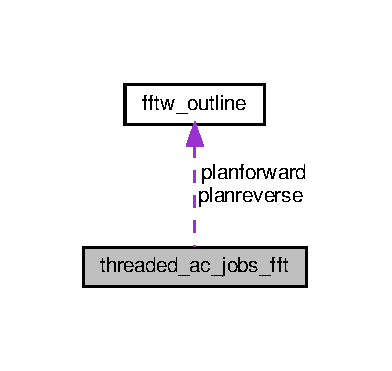
\includegraphics[width=188pt]{classthreaded__ac__jobs__fft__coll__graph}
\end{center}
\end{figure}
\subsection*{Public Attributes}
\begin{DoxyCompactItemize}
\item 
\mbox{\Hypertarget{classthreaded__ac__jobs__fft_ac4b3840c07d3dbd3f6d84371ec31e514}\label{classthreaded__ac__jobs__fft_ac4b3840c07d3dbd3f6d84371ec31e514}} 
double $\ast$$\ast$ {\bfseries data}
\item 
int $\ast$ \hyperlink{classthreaded__ac__jobs__fft_ad2c291ac1d43caab4e0c311653526d78}{length}
\item 
int $\ast$ \hyperlink{classthreaded__ac__jobs__fft_ab53d18101cba2f6e8894076aec04e033}{start}
\item 
int $\ast$ \hyperlink{classthreaded__ac__jobs__fft_a86501045468f92ae2c49b34cffe1aea3}{end}
\item 
int \hyperlink{classthreaded__ac__jobs__fft_a9bf661425ff94cfa740827b2e2affd18}{dimension}
\item 
\hyperlink{structfftw__outline}{fftw\+\_\+outline} $\ast$ \hyperlink{classthreaded__ac__jobs__fft_ac862074b94a8a1403f355110bf428cfc}{planforward}
\item 
\hyperlink{structfftw__outline}{fftw\+\_\+outline} $\ast$ \hyperlink{classthreaded__ac__jobs__fft_a9f821f5df06f0dd6b223444759143c0e}{planreverse}
\item 
int $\ast$ \hyperlink{classthreaded__ac__jobs__fft_a98153770612f6a063018be6a43cb6320}{lag}
\item 
double $\ast$ \hyperlink{classthreaded__ac__jobs__fft_a3a7fa6df5c4af8bce5820c483598fc9e}{target}
\end{DoxyCompactItemize}


\subsection{Detailed Description}
Class to contain spectral method jobs. 

\subsection{Member Data Documentation}
\mbox{\Hypertarget{classthreaded__ac__jobs__fft_a9bf661425ff94cfa740827b2e2affd18}\label{classthreaded__ac__jobs__fft_a9bf661425ff94cfa740827b2e2affd18}} 
\index{threaded\+\_\+ac\+\_\+jobs\+\_\+fft@{threaded\+\_\+ac\+\_\+jobs\+\_\+fft}!dimension@{dimension}}
\index{dimension@{dimension}!threaded\+\_\+ac\+\_\+jobs\+\_\+fft@{threaded\+\_\+ac\+\_\+jobs\+\_\+fft}}
\subsubsection{\texorpdfstring{dimension}{dimension}}
{\footnotesize\ttfamily int threaded\+\_\+ac\+\_\+jobs\+\_\+fft\+::dimension}

Read only -- end index \mbox{\Hypertarget{classthreaded__ac__jobs__fft_a86501045468f92ae2c49b34cffe1aea3}\label{classthreaded__ac__jobs__fft_a86501045468f92ae2c49b34cffe1aea3}} 
\index{threaded\+\_\+ac\+\_\+jobs\+\_\+fft@{threaded\+\_\+ac\+\_\+jobs\+\_\+fft}!end@{end}}
\index{end@{end}!threaded\+\_\+ac\+\_\+jobs\+\_\+fft@{threaded\+\_\+ac\+\_\+jobs\+\_\+fft}}
\subsubsection{\texorpdfstring{end}{end}}
{\footnotesize\ttfamily int$\ast$ threaded\+\_\+ac\+\_\+jobs\+\_\+fft\+::end}

Read only -- start index \mbox{\Hypertarget{classthreaded__ac__jobs__fft_a98153770612f6a063018be6a43cb6320}\label{classthreaded__ac__jobs__fft_a98153770612f6a063018be6a43cb6320}} 
\index{threaded\+\_\+ac\+\_\+jobs\+\_\+fft@{threaded\+\_\+ac\+\_\+jobs\+\_\+fft}!lag@{lag}}
\index{lag@{lag}!threaded\+\_\+ac\+\_\+jobs\+\_\+fft@{threaded\+\_\+ac\+\_\+jobs\+\_\+fft}}
\subsubsection{\texorpdfstring{lag}{lag}}
{\footnotesize\ttfamily int$\ast$ threaded\+\_\+ac\+\_\+jobs\+\_\+fft\+::lag}

fftw plan to use for spectral method \mbox{\Hypertarget{classthreaded__ac__jobs__fft_ad2c291ac1d43caab4e0c311653526d78}\label{classthreaded__ac__jobs__fft_ad2c291ac1d43caab4e0c311653526d78}} 
\index{threaded\+\_\+ac\+\_\+jobs\+\_\+fft@{threaded\+\_\+ac\+\_\+jobs\+\_\+fft}!length@{length}}
\index{length@{length}!threaded\+\_\+ac\+\_\+jobs\+\_\+fft@{threaded\+\_\+ac\+\_\+jobs\+\_\+fft}}
\subsubsection{\texorpdfstring{length}{length}}
{\footnotesize\ttfamily int$\ast$ threaded\+\_\+ac\+\_\+jobs\+\_\+fft\+::length}

Read only -- Data to use -- full chain \mbox{\Hypertarget{classthreaded__ac__jobs__fft_ac862074b94a8a1403f355110bf428cfc}\label{classthreaded__ac__jobs__fft_ac862074b94a8a1403f355110bf428cfc}} 
\index{threaded\+\_\+ac\+\_\+jobs\+\_\+fft@{threaded\+\_\+ac\+\_\+jobs\+\_\+fft}!planforward@{planforward}}
\index{planforward@{planforward}!threaded\+\_\+ac\+\_\+jobs\+\_\+fft@{threaded\+\_\+ac\+\_\+jobs\+\_\+fft}}
\subsubsection{\texorpdfstring{planforward}{planforward}}
{\footnotesize\ttfamily \hyperlink{structfftw__outline}{fftw\+\_\+outline}$\ast$ threaded\+\_\+ac\+\_\+jobs\+\_\+fft\+::planforward}

Read only -- dimension being analyzed \mbox{\Hypertarget{classthreaded__ac__jobs__fft_a9f821f5df06f0dd6b223444759143c0e}\label{classthreaded__ac__jobs__fft_a9f821f5df06f0dd6b223444759143c0e}} 
\index{threaded\+\_\+ac\+\_\+jobs\+\_\+fft@{threaded\+\_\+ac\+\_\+jobs\+\_\+fft}!planreverse@{planreverse}}
\index{planreverse@{planreverse}!threaded\+\_\+ac\+\_\+jobs\+\_\+fft@{threaded\+\_\+ac\+\_\+jobs\+\_\+fft}}
\subsubsection{\texorpdfstring{planreverse}{planreverse}}
{\footnotesize\ttfamily \hyperlink{structfftw__outline}{fftw\+\_\+outline}$\ast$ threaded\+\_\+ac\+\_\+jobs\+\_\+fft\+::planreverse}

fftw plan to use for spectral method \mbox{\Hypertarget{classthreaded__ac__jobs__fft_ab53d18101cba2f6e8894076aec04e033}\label{classthreaded__ac__jobs__fft_ab53d18101cba2f6e8894076aec04e033}} 
\index{threaded\+\_\+ac\+\_\+jobs\+\_\+fft@{threaded\+\_\+ac\+\_\+jobs\+\_\+fft}!start@{start}}
\index{start@{start}!threaded\+\_\+ac\+\_\+jobs\+\_\+fft@{threaded\+\_\+ac\+\_\+jobs\+\_\+fft}}
\subsubsection{\texorpdfstring{start}{start}}
{\footnotesize\ttfamily int$\ast$ threaded\+\_\+ac\+\_\+jobs\+\_\+fft\+::start}

Read only -- length of total data \mbox{\Hypertarget{classthreaded__ac__jobs__fft_a3a7fa6df5c4af8bce5820c483598fc9e}\label{classthreaded__ac__jobs__fft_a3a7fa6df5c4af8bce5820c483598fc9e}} 
\index{threaded\+\_\+ac\+\_\+jobs\+\_\+fft@{threaded\+\_\+ac\+\_\+jobs\+\_\+fft}!target@{target}}
\index{target@{target}!threaded\+\_\+ac\+\_\+jobs\+\_\+fft@{threaded\+\_\+ac\+\_\+jobs\+\_\+fft}}
\subsubsection{\texorpdfstring{target}{target}}
{\footnotesize\ttfamily double$\ast$ threaded\+\_\+ac\+\_\+jobs\+\_\+fft\+::target}

R\+E\+AD A\+ND W\+R\+I\+TE -- final lag 

The documentation for this class was generated from the following file\+:\begin{DoxyCompactItemize}
\item 
include/gwat/\hyperlink{autocorrelation_8h}{autocorrelation.\+h}\end{DoxyCompactItemize}

\hypertarget{classthreaded__ac__jobs__serial}{}\doxysection{threaded\+\_\+ac\+\_\+jobs\+\_\+serial Class Reference}
\label{classthreaded__ac__jobs__serial}\index{threaded\_ac\_jobs\_serial@{threaded\_ac\_jobs\_serial}}


Class to contain serial method jobs.  




{\ttfamily \#include $<$autocorrelation.\+h$>$}

\doxysubsection*{Public Attributes}
\begin{DoxyCompactItemize}
\item 
\mbox{\Hypertarget{classthreaded__ac__jobs__serial_acfc487b367aa6bd91dfd51a5994b89ee}\label{classthreaded__ac__jobs__serial_acfc487b367aa6bd91dfd51a5994b89ee}} 
double $\ast$$\ast$ {\bfseries data}
\item 
int $\ast$ \mbox{\hyperlink{classthreaded__ac__jobs__serial_ae6153a4df9771175723ec04d7eec03b4}{length}}
\item 
int $\ast$ \mbox{\hyperlink{classthreaded__ac__jobs__serial_a358a286626c91db48b779ee0a1be7201}{start}}
\item 
int $\ast$ \mbox{\hyperlink{classthreaded__ac__jobs__serial_afcb4978468003aae945aa2a63681b86e}{end}}
\item 
int \mbox{\hyperlink{classthreaded__ac__jobs__serial_a5ecfde8b822ea61788c90739a1a3929c}{dimension}}
\item 
int $\ast$ \mbox{\hyperlink{classthreaded__ac__jobs__serial_a6a149a8f7f02ed82c6ade734208acc0a}{lag}}
\item 
double $\ast$ \mbox{\hyperlink{classthreaded__ac__jobs__serial_a0a870c7ac95ad680d3bc8ca80f1df9f3}{target}}
\end{DoxyCompactItemize}


\doxysubsection{Detailed Description}
Class to contain serial method jobs. 

\doxysubsection{Member Data Documentation}
\mbox{\Hypertarget{classthreaded__ac__jobs__serial_a5ecfde8b822ea61788c90739a1a3929c}\label{classthreaded__ac__jobs__serial_a5ecfde8b822ea61788c90739a1a3929c}} 
\index{threaded\_ac\_jobs\_serial@{threaded\_ac\_jobs\_serial}!dimension@{dimension}}
\index{dimension@{dimension}!threaded\_ac\_jobs\_serial@{threaded\_ac\_jobs\_serial}}
\doxysubsubsection{\texorpdfstring{dimension}{dimension}}
{\footnotesize\ttfamily int threaded\+\_\+ac\+\_\+jobs\+\_\+serial\+::dimension}

Read only -- end index \mbox{\Hypertarget{classthreaded__ac__jobs__serial_afcb4978468003aae945aa2a63681b86e}\label{classthreaded__ac__jobs__serial_afcb4978468003aae945aa2a63681b86e}} 
\index{threaded\_ac\_jobs\_serial@{threaded\_ac\_jobs\_serial}!end@{end}}
\index{end@{end}!threaded\_ac\_jobs\_serial@{threaded\_ac\_jobs\_serial}}
\doxysubsubsection{\texorpdfstring{end}{end}}
{\footnotesize\ttfamily int$\ast$ threaded\+\_\+ac\+\_\+jobs\+\_\+serial\+::end}

Read only -- start index \mbox{\Hypertarget{classthreaded__ac__jobs__serial_a6a149a8f7f02ed82c6ade734208acc0a}\label{classthreaded__ac__jobs__serial_a6a149a8f7f02ed82c6ade734208acc0a}} 
\index{threaded\_ac\_jobs\_serial@{threaded\_ac\_jobs\_serial}!lag@{lag}}
\index{lag@{lag}!threaded\_ac\_jobs\_serial@{threaded\_ac\_jobs\_serial}}
\doxysubsubsection{\texorpdfstring{lag}{lag}}
{\footnotesize\ttfamily int$\ast$ threaded\+\_\+ac\+\_\+jobs\+\_\+serial\+::lag}

Read only -- dimension being analyzed \mbox{\Hypertarget{classthreaded__ac__jobs__serial_ae6153a4df9771175723ec04d7eec03b4}\label{classthreaded__ac__jobs__serial_ae6153a4df9771175723ec04d7eec03b4}} 
\index{threaded\_ac\_jobs\_serial@{threaded\_ac\_jobs\_serial}!length@{length}}
\index{length@{length}!threaded\_ac\_jobs\_serial@{threaded\_ac\_jobs\_serial}}
\doxysubsubsection{\texorpdfstring{length}{length}}
{\footnotesize\ttfamily int$\ast$ threaded\+\_\+ac\+\_\+jobs\+\_\+serial\+::length}

Read only -- Data to use -- full chain \mbox{\Hypertarget{classthreaded__ac__jobs__serial_a358a286626c91db48b779ee0a1be7201}\label{classthreaded__ac__jobs__serial_a358a286626c91db48b779ee0a1be7201}} 
\index{threaded\_ac\_jobs\_serial@{threaded\_ac\_jobs\_serial}!start@{start}}
\index{start@{start}!threaded\_ac\_jobs\_serial@{threaded\_ac\_jobs\_serial}}
\doxysubsubsection{\texorpdfstring{start}{start}}
{\footnotesize\ttfamily int$\ast$ threaded\+\_\+ac\+\_\+jobs\+\_\+serial\+::start}

Read only -- length of total data \mbox{\Hypertarget{classthreaded__ac__jobs__serial_a0a870c7ac95ad680d3bc8ca80f1df9f3}\label{classthreaded__ac__jobs__serial_a0a870c7ac95ad680d3bc8ca80f1df9f3}} 
\index{threaded\_ac\_jobs\_serial@{threaded\_ac\_jobs\_serial}!target@{target}}
\index{target@{target}!threaded\_ac\_jobs\_serial@{threaded\_ac\_jobs\_serial}}
\doxysubsubsection{\texorpdfstring{target}{target}}
{\footnotesize\ttfamily double$\ast$ threaded\+\_\+ac\+\_\+jobs\+\_\+serial\+::target}

R\+E\+AD A\+ND W\+R\+I\+TE -- final lag 

The documentation for this class was generated from the following file\+:\begin{DoxyCompactItemize}
\item 
include/gwat/\mbox{\hyperlink{autocorrelation_8h}{autocorrelation.\+h}}\end{DoxyCompactItemize}

\hypertarget{classThreadPool}{}\doxysection{Thread\+Pool Class Reference}
\label{classThreadPool}\index{ThreadPool@{ThreadPool}}
\doxysubsection*{Public Member Functions}
\begin{DoxyCompactItemize}
\item 
\mbox{\Hypertarget{classThreadPool_a9db95eb853b96e4fc832514226b4ada3}\label{classThreadPool_a9db95eb853b96e4fc832514226b4ada3}} 
{\bfseries Thread\+Pool} (std\+::size\+\_\+t num\+Threads)
\item 
\mbox{\Hypertarget{classThreadPool_adbf85eec6d088b068301338e470a9723}\label{classThreadPool_adbf85eec6d088b068301338e470a9723}} 
void {\bfseries enqueue} (int i)
\item 
\mbox{\Hypertarget{classThreadPool_acd64225bd86aa5cf7a7889c75413167e}\label{classThreadPool_acd64225bd86aa5cf7a7889c75413167e}} 
void {\bfseries enqueue\+\_\+swap} (int i)
\item 
\mbox{\Hypertarget{classThreadPool_ab85f3bf5998e7bd213326dab9895504d}\label{classThreadPool_ab85f3bf5998e7bd213326dab9895504d}} 
void {\bfseries public\+\_\+stop} ()
\end{DoxyCompactItemize}


The documentation for this class was generated from the following file\+:\begin{DoxyCompactItemize}
\item 
src/\mbox{\hyperlink{mcmc__sampler_8cpp}{mcmc\+\_\+sampler.\+cpp}}\end{DoxyCompactItemize}

\hypertarget{classThreadPool}{}\doxysection{Thread\+Pool Class Reference}
\label{classThreadPool}\index{ThreadPool@{ThreadPool}}
\doxysubsection*{Public Member Functions}
\begin{DoxyCompactItemize}
\item 
\mbox{\Hypertarget{classThreadPool_a9db95eb853b96e4fc832514226b4ada3}\label{classThreadPool_a9db95eb853b96e4fc832514226b4ada3}} 
{\bfseries Thread\+Pool} (std\+::size\+\_\+t num\+Threads)
\item 
\mbox{\Hypertarget{classThreadPool_adbf85eec6d088b068301338e470a9723}\label{classThreadPool_adbf85eec6d088b068301338e470a9723}} 
void {\bfseries enqueue} (int i)
\item 
\mbox{\Hypertarget{classThreadPool_acd64225bd86aa5cf7a7889c75413167e}\label{classThreadPool_acd64225bd86aa5cf7a7889c75413167e}} 
void {\bfseries enqueue\+\_\+swap} (int i)
\item 
\mbox{\Hypertarget{classThreadPool_ab85f3bf5998e7bd213326dab9895504d}\label{classThreadPool_ab85f3bf5998e7bd213326dab9895504d}} 
void {\bfseries public\+\_\+stop} ()
\end{DoxyCompactItemize}


The documentation for this class was generated from the following file\+:\begin{DoxyCompactItemize}
\item 
src/\mbox{\hyperlink{mcmc__sampler_8cpp}{mcmc\+\_\+sampler.\+cpp}}\end{DoxyCompactItemize}

\hypertarget{structuseful__powers}{}\section{useful\+\_\+powers$<$ T $>$ Struct Template Reference}
\label{structuseful__powers}\index{useful\+\_\+powers$<$ T $>$@{useful\+\_\+powers$<$ T $>$}}


To speed up calculations within the for loops, we pre-\/calculate reoccuring powers of M$\ast$F and Pi, since the pow() function is prohibatively slow.  




{\ttfamily \#include $<$util.\+h$>$}

\subsection*{Public Attributes}
\begin{DoxyCompactItemize}
\item 
\mbox{\Hypertarget{structuseful__powers_aa8b9ac1852ce3da063fa854b4c815e1f}\label{structuseful__powers_aa8b9ac1852ce3da063fa854b4c815e1f}} 
T {\bfseries M\+Fthird}
\item 
\mbox{\Hypertarget{structuseful__powers_a88101060465e48188fa729d3114951a7}\label{structuseful__powers_a88101060465e48188fa729d3114951a7}} 
T {\bfseries M\+Fsixth}
\item 
\mbox{\Hypertarget{structuseful__powers_a3a763d2cc229ab9f708c75447ee9cdf2}\label{structuseful__powers_a3a763d2cc229ab9f708c75447ee9cdf2}} 
T {\bfseries M\+F7sixth}
\item 
\mbox{\Hypertarget{structuseful__powers_a9929d4baac3bf8fe621202064ffa0d82}\label{structuseful__powers_a9929d4baac3bf8fe621202064ffa0d82}} 
T {\bfseries M\+F2third}
\item 
\mbox{\Hypertarget{structuseful__powers_a2d71c66517b49313e78fe71c63a279c0}\label{structuseful__powers_a2d71c66517b49313e78fe71c63a279c0}} 
T {\bfseries M\+F4third}
\item 
\mbox{\Hypertarget{structuseful__powers_a33f702a991361dc89966ce97bd87b855}\label{structuseful__powers_a33f702a991361dc89966ce97bd87b855}} 
T {\bfseries M\+F5third}
\item 
\mbox{\Hypertarget{structuseful__powers_ab94972df0a2af6417e92214baa02bf08}\label{structuseful__powers_ab94972df0a2af6417e92214baa02bf08}} 
T {\bfseries M\+Fsquare}
\item 
\mbox{\Hypertarget{structuseful__powers_ace3dd7ac047c4d4c1962f3e0fb9ee22f}\label{structuseful__powers_ace3dd7ac047c4d4c1962f3e0fb9ee22f}} 
T {\bfseries M\+F7third}
\item 
\mbox{\Hypertarget{structuseful__powers_a8f1b657d0bc29739d9f0a6b57347a605}\label{structuseful__powers_a8f1b657d0bc29739d9f0a6b57347a605}} 
T {\bfseries M\+F8third}
\item 
\mbox{\Hypertarget{structuseful__powers_acfcb3477b631f8cdc767cccf0cff0c87}\label{structuseful__powers_acfcb3477b631f8cdc767cccf0cff0c87}} 
T {\bfseries M\+Fcube}
\item 
\mbox{\Hypertarget{structuseful__powers_a03cc4eaa07be77b91dec7cc49bb74d37}\label{structuseful__powers_a03cc4eaa07be77b91dec7cc49bb74d37}} 
T {\bfseries M\+Fminus\+\_\+5third}
\item 
\mbox{\Hypertarget{structuseful__powers_ab1a613f9533efdad50a379f1a50f80a1}\label{structuseful__powers_ab1a613f9533efdad50a379f1a50f80a1}} 
T {\bfseries M\+F3fourth}
\item 
\mbox{\Hypertarget{structuseful__powers_a17019be1f43fc88a0a8906c0b0c86179}\label{structuseful__powers_a17019be1f43fc88a0a8906c0b0c86179}} 
double {\bfseries P\+Isquare}
\item 
\mbox{\Hypertarget{structuseful__powers_abf93d647fb55848266bfa179a6118c22}\label{structuseful__powers_abf93d647fb55848266bfa179a6118c22}} 
double {\bfseries P\+Icube}
\item 
\mbox{\Hypertarget{structuseful__powers_a4b48e36e3acf84d91a81fe1cc8d9a7a7}\label{structuseful__powers_a4b48e36e3acf84d91a81fe1cc8d9a7a7}} 
double {\bfseries P\+Ithird}
\item 
\mbox{\Hypertarget{structuseful__powers_acb8ebe3afa5700faabee08772532f11e}\label{structuseful__powers_acb8ebe3afa5700faabee08772532f11e}} 
double {\bfseries P\+I2third}
\item 
\mbox{\Hypertarget{structuseful__powers_ab980b3eea9af1225b75450837c6da7ab}\label{structuseful__powers_ab980b3eea9af1225b75450837c6da7ab}} 
double {\bfseries P\+I4third}
\item 
\mbox{\Hypertarget{structuseful__powers_a844f8ca2f137bdd2bd51bcacb8a11fd0}\label{structuseful__powers_a844f8ca2f137bdd2bd51bcacb8a11fd0}} 
double {\bfseries P\+I5third}
\item 
\mbox{\Hypertarget{structuseful__powers_a398b4320fabb77a71a6cfb942ccf4fb8}\label{structuseful__powers_a398b4320fabb77a71a6cfb942ccf4fb8}} 
double {\bfseries P\+I7third}
\item 
\mbox{\Hypertarget{structuseful__powers_a4053c92711daa53f53a1e46d239cf19e}\label{structuseful__powers_a4053c92711daa53f53a1e46d239cf19e}} 
double {\bfseries P\+Iminus\+\_\+5third}
\end{DoxyCompactItemize}


\subsection{Detailed Description}
\subsubsection*{template$<$class T$>$\newline
struct useful\+\_\+powers$<$ T $>$}

To speed up calculations within the for loops, we pre-\/calculate reoccuring powers of M$\ast$F and Pi, since the pow() function is prohibatively slow. 

Powers of PI are initialized once, and powers of MF need to be calculated once per for loop (if in the inspiral portion).

use the functions precalc\+\_\+powers\+\_\+ins\+\_\+amp, precalc\+\_\+powers\+\_\+ins\+\_\+phase, precalc\+\_\+powers\+\_\+pi to initialize 

The documentation for this struct was generated from the following file\+:\begin{DoxyCompactItemize}
\item 
include/gwat/\hyperlink{util_8h}{util.\+h}\end{DoxyCompactItemize}

\chapter{File Documentation}
\hypertarget{autocorrelation_8h}{}\doxysection{include/gwat/autocorrelation.h File Reference}
\label{autocorrelation_8h}\index{include/gwat/autocorrelation.h@{include/gwat/autocorrelation.h}}
{\ttfamily \#include $<$string$>$}\newline
{\ttfamily \#include \char`\"{}util.\+h\char`\"{}}\newline
Include dependency graph for autocorrelation.\+h\+:

\hypertarget{autocorrelation__cuda_8h}{}\doxysection{include/gwat/autocorrelation\+\_\+cuda.h File Reference}
\label{autocorrelation__cuda_8h}\index{include/gwat/autocorrelation\_cuda.h@{include/gwat/autocorrelation\_cuda.h}}
{\ttfamily \#include $<$string$>$}\newline
Include dependency graph for autocorrelation\+\_\+cuda.\+h\+:
\nopagebreak
\begin{figure}[H]
\begin{center}
\leavevmode
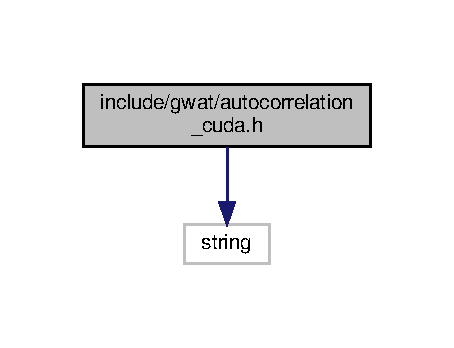
\includegraphics[width=218pt]{autocorrelation__cuda_8h__incl}
\end{center}
\end{figure}
This graph shows which files directly or indirectly include this file\+:
\nopagebreak
\begin{figure}[H]
\begin{center}
\leavevmode
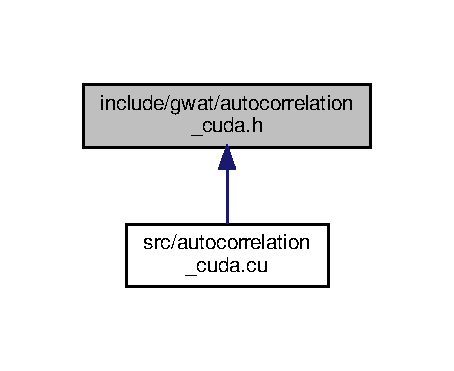
\includegraphics[width=218pt]{autocorrelation__cuda_8h__dep__incl}
\end{center}
\end{figure}
\doxysubsection*{Macros}
\begin{DoxyCompactItemize}
\item 
\mbox{\Hypertarget{autocorrelation__cuda_8h_a869bf6501bf4809f3de1db59ef2dd914}\label{autocorrelation__cuda_8h_a869bf6501bf4809f3de1db59ef2dd914}} 
\#define {\bfseries T\+H\+R\+E\+A\+D\+S\+\_\+\+P\+E\+R\+\_\+\+B\+L\+O\+CK}~512
\end{DoxyCompactItemize}
\doxysubsection*{Functions}
\begin{DoxyCompactItemize}
\item 
void \mbox{\hyperlink{autocorrelation__cuda_8h_a4b4ed2b89a95a13abf59d6e373316770}{write\+\_\+file\+\_\+auto\+\_\+corr\+\_\+from\+\_\+data\+\_\+file\+\_\+accel}} (std\+::string acfile, std\+::string chains\+\_\+file, int dimension, int N\+\_\+steps, int num\+\_\+segments, double target\+\_\+corr)
\begin{DoxyCompactList}\small\item\em Write data file for autocorrelation lengths of the data given a data file name, as written by the mcmc\+\_\+sampler. \end{DoxyCompactList}\item 
void \mbox{\hyperlink{autocorrelation__cuda_8h_a4e58f577dbd00180667c1a6452f4cd71}{write\+\_\+file\+\_\+auto\+\_\+corr\+\_\+from\+\_\+data\+\_\+accel}} (std\+::string acfile, double $\ast$$\ast$output, int dimension, int N\+\_\+steps, int num\+\_\+segments, double target\+\_\+corr)
\begin{DoxyCompactList}\small\item\em Write data file given output chains, as formatted by the mcmc\+\_\+sampler. \end{DoxyCompactList}\item 
void \mbox{\hyperlink{autocorrelation__cuda_8h_a32229785a7faa2b81d4894aafc640ed5}{auto\+\_\+corr\+\_\+from\+\_\+data\+\_\+accel}} (double $\ast$$\ast$output, int dimension, int N\+\_\+steps, int num\+\_\+segments, double target\+\_\+corr, double $\ast$$\ast$autocorr)
\begin{DoxyCompactList}\small\item\em Find autocorrelation of data at different points in the chain length and output to autocorr. \end{DoxyCompactList}\item 
\mbox{\Hypertarget{autocorrelation__cuda_8h_a3cf30342474041a00ac261eb5e7afed3}\label{autocorrelation__cuda_8h_a3cf30342474041a00ac261eb5e7afed3}} 
void \mbox{\hyperlink{autocorrelation__cuda_8h_a3cf30342474041a00ac261eb5e7afed3}{launch\+\_\+ac\+\_\+gpu}} (int device, int element, double $\ast$$\ast$data, int length, int dimension, double target\+\_\+corr, int num\+\_\+segments)
\begin{DoxyCompactList}\small\item\em Launch the G\+PU kernel, formatted for the thread pool. \end{DoxyCompactList}\item 
void \mbox{\hyperlink{autocorrelation__cuda_8h_a51bcc72596ce81494ca39a8aa7a74c53}{ac\+\_\+gpu\+\_\+wrapper}} (int thread, int job\+\_\+id)
\begin{DoxyCompactList}\small\item\em Wrapper function for the thread pool. \end{DoxyCompactList}\item 
\mbox{\Hypertarget{autocorrelation__cuda_8h_a0128283c572fef800902137f1fc763e6}\label{autocorrelation__cuda_8h_a0128283c572fef800902137f1fc763e6}} 
void {\bfseries auto\+\_\+correlation\+\_\+spectral\+\_\+accel} (double $\ast$chains, int length, double $\ast$autocorr)
\end{DoxyCompactItemize}


\doxysubsection{Detailed Description}
Header file for C\+U\+DA accelerated algorithms

Currently, no algorithms are used in any other parts of the project, so if C\+U\+DA or C\+U\+D\+A-\/enabled devices are not available, this file can be skipped in compilation by commenting out the O\+B\+J\+E\+C\+T\+S\+C\+U\+DA line in the makefile 

\doxysubsection{Function Documentation}
\mbox{\Hypertarget{autocorrelation__cuda_8h_a51bcc72596ce81494ca39a8aa7a74c53}\label{autocorrelation__cuda_8h_a51bcc72596ce81494ca39a8aa7a74c53}} 
\index{autocorrelation\_cuda.h@{autocorrelation\_cuda.h}!ac\_gpu\_wrapper@{ac\_gpu\_wrapper}}
\index{ac\_gpu\_wrapper@{ac\_gpu\_wrapper}!autocorrelation\_cuda.h@{autocorrelation\_cuda.h}}
\doxysubsubsection{\texorpdfstring{ac\_gpu\_wrapper()}{ac\_gpu\_wrapper()}}
{\footnotesize\ttfamily void ac\+\_\+gpu\+\_\+wrapper (\begin{DoxyParamCaption}\item[{int}]{thread,  }\item[{int}]{job\+\_\+id }\end{DoxyParamCaption})}



Wrapper function for the thread pool. 


\begin{DoxyParams}{Parameters}
{\em thread} & Host thread \\
\hline
{\em job\+\_\+id} & Job ID \\
\hline
\end{DoxyParams}
\mbox{\Hypertarget{autocorrelation__cuda_8h_a32229785a7faa2b81d4894aafc640ed5}\label{autocorrelation__cuda_8h_a32229785a7faa2b81d4894aafc640ed5}} 
\index{autocorrelation\_cuda.h@{autocorrelation\_cuda.h}!auto\_corr\_from\_data\_accel@{auto\_corr\_from\_data\_accel}}
\index{auto\_corr\_from\_data\_accel@{auto\_corr\_from\_data\_accel}!autocorrelation\_cuda.h@{autocorrelation\_cuda.h}}
\doxysubsubsection{\texorpdfstring{auto\_corr\_from\_data\_accel()}{auto\_corr\_from\_data\_accel()}}
{\footnotesize\ttfamily void auto\+\_\+corr\+\_\+from\+\_\+data\+\_\+accel (\begin{DoxyParamCaption}\item[{double $\ast$$\ast$}]{output,  }\item[{int}]{dimension,  }\item[{int}]{N\+\_\+steps,  }\item[{int}]{num\+\_\+segments,  }\item[{double}]{target\+\_\+corr,  }\item[{double $\ast$$\ast$}]{autocorr }\end{DoxyParamCaption})}



Find autocorrelation of data at different points in the chain length and output to autocorr. 


\begin{DoxyParams}[1]{Parameters}
 & {\em output} & Chain data input \\
\hline
 & {\em dimension} & Dimension of the data \\
\hline
 & {\em N\+\_\+steps} & Number of steps in the data \\
\hline
 & {\em num\+\_\+segments} & number of segments to calculate the autocorrelation length \\
\hline
 & {\em target\+\_\+corr} & Target correlation ratio \\
\hline
\mbox{\texttt{ out}}  & {\em autocorr} & Autocorrelation lengths for the different segments \\
\hline
\end{DoxyParams}
\mbox{\Hypertarget{autocorrelation__cuda_8h_a4e58f577dbd00180667c1a6452f4cd71}\label{autocorrelation__cuda_8h_a4e58f577dbd00180667c1a6452f4cd71}} 
\index{autocorrelation\_cuda.h@{autocorrelation\_cuda.h}!write\_file\_auto\_corr\_from\_data\_accel@{write\_file\_auto\_corr\_from\_data\_accel}}
\index{write\_file\_auto\_corr\_from\_data\_accel@{write\_file\_auto\_corr\_from\_data\_accel}!autocorrelation\_cuda.h@{autocorrelation\_cuda.h}}
\doxysubsubsection{\texorpdfstring{write\_file\_auto\_corr\_from\_data\_accel()}{write\_file\_auto\_corr\_from\_data\_accel()}}
{\footnotesize\ttfamily void write\+\_\+file\+\_\+auto\+\_\+corr\+\_\+from\+\_\+data\+\_\+accel (\begin{DoxyParamCaption}\item[{std\+::string}]{acfile,  }\item[{double $\ast$$\ast$}]{output,  }\item[{int}]{dimension,  }\item[{int}]{N\+\_\+steps,  }\item[{int}]{num\+\_\+segments,  }\item[{double}]{target\+\_\+corr }\end{DoxyParamCaption})}



Write data file given output chains, as formatted by the mcmc\+\_\+sampler. 


\begin{DoxyParams}{Parameters}
{\em acfile} & Output autocorrelation filename \\
\hline
{\em output} & Chain data from M\+C\+M\+C\+\_\+sampler \\
\hline
{\em dimension} & Dimension of the data \\
\hline
{\em N\+\_\+steps} & Number of steps in the chain \\
\hline
{\em num\+\_\+segments} & Number of segments to check the autocorrelation length for each dimension \\
\hline
{\em target\+\_\+corr} & Target correlation ratio to use for the correlation length calculation \\
\hline
\end{DoxyParams}
\mbox{\Hypertarget{autocorrelation__cuda_8h_a4b4ed2b89a95a13abf59d6e373316770}\label{autocorrelation__cuda_8h_a4b4ed2b89a95a13abf59d6e373316770}} 
\index{autocorrelation\_cuda.h@{autocorrelation\_cuda.h}!write\_file\_auto\_corr\_from\_data\_file\_accel@{write\_file\_auto\_corr\_from\_data\_file\_accel}}
\index{write\_file\_auto\_corr\_from\_data\_file\_accel@{write\_file\_auto\_corr\_from\_data\_file\_accel}!autocorrelation\_cuda.h@{autocorrelation\_cuda.h}}
\doxysubsubsection{\texorpdfstring{write\_file\_auto\_corr\_from\_data\_file\_accel()}{write\_file\_auto\_corr\_from\_data\_file\_accel()}}
{\footnotesize\ttfamily void write\+\_\+file\+\_\+auto\+\_\+corr\+\_\+from\+\_\+data\+\_\+file\+\_\+accel (\begin{DoxyParamCaption}\item[{std\+::string}]{acfile,  }\item[{std\+::string}]{chains\+\_\+file,  }\item[{int}]{dimension,  }\item[{int}]{N\+\_\+steps,  }\item[{int}]{num\+\_\+segments,  }\item[{double}]{target\+\_\+corr }\end{DoxyParamCaption})}



Write data file for autocorrelation lengths of the data given a data file name, as written by the mcmc\+\_\+sampler. 


\begin{DoxyParams}{Parameters}
{\em acfile} & Filename of the autocorrelation data \\
\hline
{\em chains\+\_\+file} & Filename of the data file for the chains \\
\hline
{\em dimension} & Dimension of the data \\
\hline
{\em N\+\_\+steps} & Number of steps in the chain \\
\hline
{\em num\+\_\+segments} & Number of segments to check the autocorrelation length for each dimension \\
\hline
{\em target\+\_\+corr} & Target correlation ratio to use for the correlation length calculation \\
\hline
\end{DoxyParams}

\hypertarget{autocorrelation__cuda_8hu}{}\doxysection{include/gwat/autocorrelation\+\_\+cuda.hu File Reference}
\label{autocorrelation__cuda_8hu}\index{include/gwat/autocorrelation\_cuda.hu@{include/gwat/autocorrelation\_cuda.hu}}
This graph shows which files directly or indirectly include this file\+:
\nopagebreak
\begin{figure}[H]
\begin{center}
\leavevmode
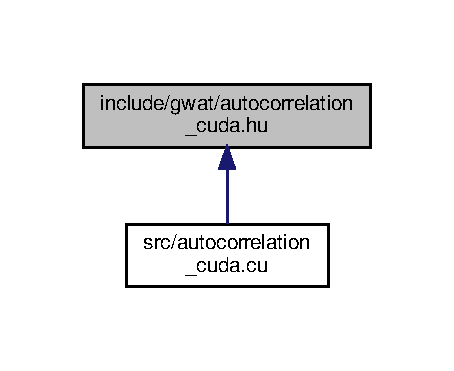
\includegraphics[width=218pt]{autocorrelation__cuda_8hu__dep__incl}
\end{center}
\end{figure}
\doxysubsection*{Classes}
\begin{DoxyCompactItemize}
\item 
struct \mbox{\hyperlink{structGPUplan}{G\+P\+Uplan}}
\end{DoxyCompactItemize}
\doxysubsection*{Functions}
\begin{DoxyCompactItemize}
\item 
\+\_\+\+\_\+device\+\_\+\+\_\+ \+\_\+\+\_\+host\+\_\+\+\_\+ void \mbox{\hyperlink{autocorrelation__cuda_8hu_a366f884938ea0477409e8d52f0309a44}{auto\+\_\+corr\+\_\+internal}} (double $\ast$arr, int length, int lag, double average, double $\ast$corr, int start\+\_\+id)
\begin{DoxyCompactList}\small\item\em Internal function to calculate the autocorrelation for a given lag Customized for the thread pool architecture, with extra arguments because of the way the memory is allocated. \end{DoxyCompactList}\item 
\+\_\+\+\_\+global\+\_\+\+\_\+ void \mbox{\hyperlink{autocorrelation__cuda_8hu_ad8cff0e627281b397e017fec619b38a5}{auto\+\_\+corr\+\_\+internal\+\_\+kernal}} (double $\ast$arr, int length, double average, int $\ast$rho\+\_\+index, double target\+\_\+corr, double var, int start\+\_\+id)
\begin{DoxyCompactList}\small\item\em Internal function to launch the C\+U\+DA kernel for a range of autocorrelations. \end{DoxyCompactList}\item 
void \mbox{\hyperlink{autocorrelation__cuda_8hu_a0516461a0e02bf12da6c199061247a77}{allocate\+\_\+gpu\+\_\+plan}} (\mbox{\hyperlink{structGPUplan}{G\+P\+Uplan}} $\ast$plan, int data\+\_\+length, int dimension, int num\+\_\+segments)
\begin{DoxyCompactList}\small\item\em Allocates memory for autocorrelation--G\+PU structure. \end{DoxyCompactList}\item 
void \mbox{\hyperlink{autocorrelation__cuda_8hu_a131867ca45185be0af927a5ec7d7645d}{deallocate\+\_\+gpu\+\_\+plan}} (\mbox{\hyperlink{structGPUplan}{G\+P\+Uplan}} $\ast$plan, int data\+\_\+length, int dimension, int num\+\_\+segments)
\begin{DoxyCompactList}\small\item\em Deallocates memory for the autocorrelation--G\+PU structure. \end{DoxyCompactList}\item 
void \mbox{\hyperlink{autocorrelation__cuda_8hu_a00159a0e9eb7e40725a034becb3110c0}{copy\+\_\+data\+\_\+to\+\_\+device}} (\mbox{\hyperlink{structGPUplan}{G\+P\+Uplan}} $\ast$plan, double $\ast$$\ast$input\+\_\+data, int data\+\_\+length, int dimension, int num\+\_\+segments)
\begin{DoxyCompactList}\small\item\em Copy data to device before starting kernels. \end{DoxyCompactList}\end{DoxyCompactItemize}


\doxysubsection{Function Documentation}
\mbox{\Hypertarget{autocorrelation__cuda_8hu_a0516461a0e02bf12da6c199061247a77}\label{autocorrelation__cuda_8hu_a0516461a0e02bf12da6c199061247a77}} 
\index{autocorrelation\_cuda.hu@{autocorrelation\_cuda.hu}!allocate\_gpu\_plan@{allocate\_gpu\_plan}}
\index{allocate\_gpu\_plan@{allocate\_gpu\_plan}!autocorrelation\_cuda.hu@{autocorrelation\_cuda.hu}}
\doxysubsubsection{\texorpdfstring{allocate\_gpu\_plan()}{allocate\_gpu\_plan()}}
{\footnotesize\ttfamily void allocate\+\_\+gpu\+\_\+plan (\begin{DoxyParamCaption}\item[{\mbox{\hyperlink{structGPUplan}{G\+P\+Uplan}} $\ast$}]{plan,  }\item[{int}]{data\+\_\+length,  }\item[{int}]{dimension,  }\item[{int}]{num\+\_\+segments }\end{DoxyParamCaption})}



Allocates memory for autocorrelation--G\+PU structure. 


\begin{DoxyParams}{Parameters}
{\em plan} & Structure for G\+PU plan \\
\hline
{\em data\+\_\+length} & Length of data \\
\hline
{\em dimension} & Dimension of the data \\
\hline
{\em num\+\_\+segments} & Number of segments to calculate the autocorrelation length \\
\hline
\end{DoxyParams}
\mbox{\Hypertarget{autocorrelation__cuda_8hu_a366f884938ea0477409e8d52f0309a44}\label{autocorrelation__cuda_8hu_a366f884938ea0477409e8d52f0309a44}} 
\index{autocorrelation\_cuda.hu@{autocorrelation\_cuda.hu}!auto\_corr\_internal@{auto\_corr\_internal}}
\index{auto\_corr\_internal@{auto\_corr\_internal}!autocorrelation\_cuda.hu@{autocorrelation\_cuda.hu}}
\doxysubsubsection{\texorpdfstring{auto\_corr\_internal()}{auto\_corr\_internal()}}
{\footnotesize\ttfamily \+\_\+\+\_\+device\+\_\+\+\_\+ \+\_\+\+\_\+host\+\_\+\+\_\+ void auto\+\_\+corr\+\_\+internal (\begin{DoxyParamCaption}\item[{double $\ast$}]{arr,  }\item[{int}]{length,  }\item[{int}]{lag,  }\item[{double}]{average,  }\item[{double $\ast$}]{corr,  }\item[{int}]{start\+\_\+id }\end{DoxyParamCaption})}



Internal function to calculate the autocorrelation for a given lag Customized for the thread pool architecture, with extra arguments because of the way the memory is allocated. 


\begin{DoxyParams}[1]{Parameters}
 & {\em arr} & Input array of data \\
\hline
 & {\em length} & Length of input array \\
\hline
 & {\em lag} & Lag to be used to calculate the correlation \\
\hline
 & {\em average} & Average of the array arr \\
\hline
\mbox{\texttt{ out}}  & {\em corr} & output correlation \\
\hline
 & {\em start\+\_\+id} & ID of location to start calculation -\/-\/ input arrary arr is assumed to be contiguous for multiple dimensions \\
\hline
\end{DoxyParams}
\mbox{\Hypertarget{autocorrelation__cuda_8hu_ad8cff0e627281b397e017fec619b38a5}\label{autocorrelation__cuda_8hu_ad8cff0e627281b397e017fec619b38a5}} 
\index{autocorrelation\_cuda.hu@{autocorrelation\_cuda.hu}!auto\_corr\_internal\_kernal@{auto\_corr\_internal\_kernal}}
\index{auto\_corr\_internal\_kernal@{auto\_corr\_internal\_kernal}!autocorrelation\_cuda.hu@{autocorrelation\_cuda.hu}}
\doxysubsubsection{\texorpdfstring{auto\_corr\_internal\_kernal()}{auto\_corr\_internal\_kernal()}}
{\footnotesize\ttfamily \+\_\+\+\_\+global\+\_\+\+\_\+ void auto\+\_\+corr\+\_\+internal\+\_\+kernal (\begin{DoxyParamCaption}\item[{double $\ast$}]{arr,  }\item[{int}]{length,  }\item[{double}]{average,  }\item[{int $\ast$}]{rho\+\_\+index,  }\item[{double}]{target\+\_\+corr,  }\item[{double}]{var,  }\item[{int}]{start\+\_\+id }\end{DoxyParamCaption})}



Internal function to launch the C\+U\+DA kernel for a range of autocorrelations. 

Correlation function used\+:

rho(lag) = 1 / (length -\/ lag) \textbackslash{}sum (arr\mbox{[}i+lag\mbox{]}-\/average) ( arr\mbox{[}i\mbox{]}-\/ average)

target\+\_\+corr = rho(rho\+\_\+index)/rho(0) = rho(rho\+\_\+index)/var 
\begin{DoxyParams}[1]{Parameters}
 & {\em arr} & Input array of data \\
\hline
 & {\em length} & Length of data array \\
\hline
 & {\em average} & Average of input data \\
\hline
\mbox{\texttt{ out}}  & {\em rho\+\_\+index} & Index of the lag that results ina correlation ratio target\+\_\+corr \\
\hline
 & {\em target\+\_\+corr} & Target correlation ratio rho(lag)/rho(0) = target\+\_\+corr \\
\hline
 & {\em var} & Variance rho(0) \\
\hline
 & {\em start\+\_\+id} & Starting index to use for the data array arr \\
\hline
\end{DoxyParams}
\mbox{\Hypertarget{autocorrelation__cuda_8hu_a00159a0e9eb7e40725a034becb3110c0}\label{autocorrelation__cuda_8hu_a00159a0e9eb7e40725a034becb3110c0}} 
\index{autocorrelation\_cuda.hu@{autocorrelation\_cuda.hu}!copy\_data\_to\_device@{copy\_data\_to\_device}}
\index{copy\_data\_to\_device@{copy\_data\_to\_device}!autocorrelation\_cuda.hu@{autocorrelation\_cuda.hu}}
\doxysubsubsection{\texorpdfstring{copy\_data\_to\_device()}{copy\_data\_to\_device()}}
{\footnotesize\ttfamily void copy\+\_\+data\+\_\+to\+\_\+device (\begin{DoxyParamCaption}\item[{\mbox{\hyperlink{structGPUplan}{G\+P\+Uplan}} $\ast$}]{plan,  }\item[{double $\ast$$\ast$}]{input\+\_\+data,  }\item[{int}]{data\+\_\+length,  }\item[{int}]{dimension,  }\item[{int}]{num\+\_\+segments }\end{DoxyParamCaption})}



Copy data to device before starting kernels. 


\begin{DoxyParams}{Parameters}
{\em plan} & G\+PU plan \\
\hline
{\em input\+\_\+data} & Input chain data \\
\hline
{\em data\+\_\+length} & Length of data \\
\hline
{\em dimension} & Dimension of the data \\
\hline
{\em num\+\_\+segments} & Number of segments to calculate the autocorrelation length \\
\hline
\end{DoxyParams}
\mbox{\Hypertarget{autocorrelation__cuda_8hu_a131867ca45185be0af927a5ec7d7645d}\label{autocorrelation__cuda_8hu_a131867ca45185be0af927a5ec7d7645d}} 
\index{autocorrelation\_cuda.hu@{autocorrelation\_cuda.hu}!deallocate\_gpu\_plan@{deallocate\_gpu\_plan}}
\index{deallocate\_gpu\_plan@{deallocate\_gpu\_plan}!autocorrelation\_cuda.hu@{autocorrelation\_cuda.hu}}
\doxysubsubsection{\texorpdfstring{deallocate\_gpu\_plan()}{deallocate\_gpu\_plan()}}
{\footnotesize\ttfamily void deallocate\+\_\+gpu\+\_\+plan (\begin{DoxyParamCaption}\item[{\mbox{\hyperlink{structGPUplan}{G\+P\+Uplan}} $\ast$}]{plan,  }\item[{int}]{data\+\_\+length,  }\item[{int}]{dimension,  }\item[{int}]{num\+\_\+segments }\end{DoxyParamCaption})}



Deallocates memory for the autocorrelation--G\+PU structure. 


\begin{DoxyParams}{Parameters}
{\em plan} & Structure for the G\+PU plan \\
\hline
{\em data\+\_\+length} & Length of data \\
\hline
{\em dimension} & Dimension of the data \\
\hline
{\em num\+\_\+segments} & Number of segments to calculate the autocorrelation length \\
\hline
\end{DoxyParams}

\hypertarget{D__Z__Config_8h}{}\section{include/gwat/\+D\+\_\+\+Z\+\_\+\+Config.h File Reference}
\label{D__Z__Config_8h}\index{include/gwat/\+D\+\_\+\+Z\+\_\+\+Config.\+h@{include/gwat/\+D\+\_\+\+Z\+\_\+\+Config.\+h}}
This graph shows which files directly or indirectly include this file\+:\nopagebreak
\begin{figure}[H]
\begin{center}
\leavevmode
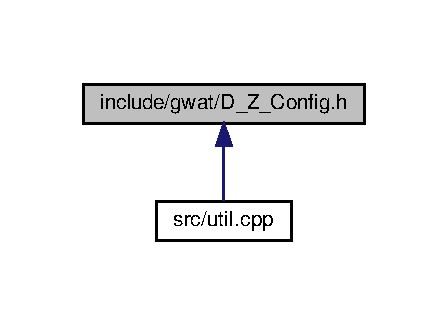
\includegraphics[width=215pt]{D__Z__Config_8h__dep__incl}
\end{center}
\end{figure}
\subsection*{Variables}
\begin{DoxyCompactItemize}
\item 
\mbox{\Hypertarget{D__Z__Config_8h_af9a72739b041969ce7ad89d7e98b25d8}\label{D__Z__Config_8h_af9a72739b041969ce7ad89d7e98b25d8}} 
const char $\ast$ {\bfseries cosmos} \mbox{[}6\mbox{]} = \{\char`\"{}P\+L\+A\+N\+C\+K15\char`\"{}, \char`\"{}P\+L\+A\+N\+C\+K13\char`\"{}, \char`\"{}W\+M\+A\+P9\char`\"{}, \char`\"{}W\+M\+A\+P7\char`\"{}, \char`\"{}W\+M\+A\+P5\char`\"{}, \char`\"{}T\+E\+S\+T\+I\+N\+G\+\_\+\+C\+O\+S\+M\+O\+L\+O\+GY\char`\"{}\}
\item 
\mbox{\Hypertarget{D__Z__Config_8h_ab840006783f40488f6fd20cc49023a83}\label{D__Z__Config_8h_ab840006783f40488f6fd20cc49023a83}} 
const int {\bfseries num\+\_\+cosmologies} = 6
\item 
\mbox{\Hypertarget{D__Z__Config_8h_aac953daa8839736a9045defba4330a71}\label{D__Z__Config_8h_aac953daa8839736a9045defba4330a71}} 
const int {\bfseries num\+\_\+segments} \mbox{[}6\mbox{]} = \{ 3, 3, 3, 3, 3, 3\}
\item 
\mbox{\Hypertarget{D__Z__Config_8h_afc1873cc6648007ce72f0af60d04b4db}\label{D__Z__Config_8h_afc1873cc6648007ce72f0af60d04b4db}} 
const int {\bfseries interp\+\_\+degree} \mbox{[}6\mbox{]} = \{ 12, 12, 12, 12, 12, 12\}
\item 
const double {\bfseries boundaries\+\_\+Z} \mbox{[}6\mbox{]}\mbox{[}4\mbox{]}
\item 
const double {\bfseries boundaries\+\_\+D} \mbox{[}6\mbox{]}\mbox{[}4\mbox{]}
\item 
\mbox{\Hypertarget{D__Z__Config_8h_a07c571b42ef6b98e3c8cc518c79ceeff}\label{D__Z__Config_8h_a07c571b42ef6b98e3c8cc518c79ceeff}} 
const double {\bfseries C\+O\+E\+F\+F\+\_\+\+V\+E\+C\+\_\+\+DZ} \mbox{[}6\mbox{]}\mbox{[}3\mbox{]}\mbox{[}12\mbox{]}
\item 
\mbox{\Hypertarget{D__Z__Config_8h_a412639ff29e5a03d1fcc3e3ad3485e91}\label{D__Z__Config_8h_a412639ff29e5a03d1fcc3e3ad3485e91}} 
const double {\bfseries C\+O\+E\+F\+F\+\_\+\+V\+E\+C\+\_\+\+ZD} \mbox{[}6\mbox{]}\mbox{[}3\mbox{]}\mbox{[}12\mbox{]}
\end{DoxyCompactItemize}


\subsection{Detailed Description}

\begin{DoxyItemize}
\item Header file for the cosmological interpolation 
\end{DoxyItemize}

\subsection{Variable Documentation}
\mbox{\Hypertarget{D__Z__Config_8h_a1bda94f9c8a2915efd2ef351225a3e78}\label{D__Z__Config_8h_a1bda94f9c8a2915efd2ef351225a3e78}} 
\index{D\+\_\+\+Z\+\_\+\+Config.\+h@{D\+\_\+\+Z\+\_\+\+Config.\+h}!boundaries\+\_\+D@{boundaries\+\_\+D}}
\index{boundaries\+\_\+D@{boundaries\+\_\+D}!D\+\_\+\+Z\+\_\+\+Config.\+h@{D\+\_\+\+Z\+\_\+\+Config.\+h}}
\subsubsection{\texorpdfstring{boundaries\+\_\+D}{boundaries\_D}}
{\footnotesize\ttfamily const double boundaries\+\_\+D\mbox{[}6\mbox{]}\mbox{[}4\mbox{]}}

{\bfseries Initial value\+:}
\begin{DoxyCode}
= \{\{1.2015524178010442
, 1.2015524178010442
, 344.0498142197095
, 230421.91551573356
\},\{1.201020615326616
, 1.201020615326616
, 343.9047300972533
, 230427.0888269416
\},\{1.17417097464182
, 1.17417097464182
, 336.6234405707774
, 231610.64191786345
\},\{1.1561615382304566
, 1.1561615382304566
, 331.7253154763896
, 232528.33987307717
\},\{1.1594542653630548
, 1.1594542653630548
, 332.57833550529614
, 231611.2292384872
\},\{1.1627615740723667
, 1.1627615740723667
, 333.1073436849841
, 225588.22699222033
\}\}
\end{DoxyCode}
\mbox{\Hypertarget{D__Z__Config_8h_ae70235cdcbcd1ff07238aecee1d92c96}\label{D__Z__Config_8h_ae70235cdcbcd1ff07238aecee1d92c96}} 
\index{D\+\_\+\+Z\+\_\+\+Config.\+h@{D\+\_\+\+Z\+\_\+\+Config.\+h}!boundaries\+\_\+Z@{boundaries\+\_\+Z}}
\index{boundaries\+\_\+Z@{boundaries\+\_\+Z}!D\+\_\+\+Z\+\_\+\+Config.\+h@{D\+\_\+\+Z\+\_\+\+Config.\+h}}
\subsubsection{\texorpdfstring{boundaries\+\_\+Z}{boundaries\_Z}}
{\footnotesize\ttfamily const double boundaries\+\_\+Z\mbox{[}6\mbox{]}\mbox{[}4\mbox{]}}

{\bfseries Initial value\+:}
\begin{DoxyCode}
= \{\{0.00027144176165949066
, 0.00027144176165949066
, 0.07368062997280773
, 20.000000000000004
\},\{0.00027144176165949066
, 0.00027144176165949066
, 0.07368062997280773
, 20.000000000000004
\},\{0.00027144176165949066
, 0.00027144176165949066
, 0.07368062997280773
, 20.000000000000004
\},\{0.00027144176165949066
, 0.00027144176165949066
, 0.07368062997280773
, 20.000000000000004
\},\{0.00027144176165949066
, 0.00027144176165949066
, 0.07368062997280773
, 20.000000000000004
\},\{0.00027144176165949066
, 0.00027144176165949066
, 0.07368062997280773
, 20.000000000000004
\}\}
\end{DoxyCode}

\hypertarget{detector__util_8h}{}\section{include/gwat/detector\+\_\+util.h File Reference}
\label{detector__util_8h}\index{include/gwat/detector\+\_\+util.\+h@{include/gwat/detector\+\_\+util.\+h}}
{\ttfamily \#include $<$string$>$}\newline
{\ttfamily \#include $<$complex$>$}\newline
{\ttfamily \#include \char`\"{}util.\+h\char`\"{}}\newline
Include dependency graph for detector\+\_\+util.\+h\+:\nopagebreak
\begin{figure}[H]
\begin{center}
\leavevmode
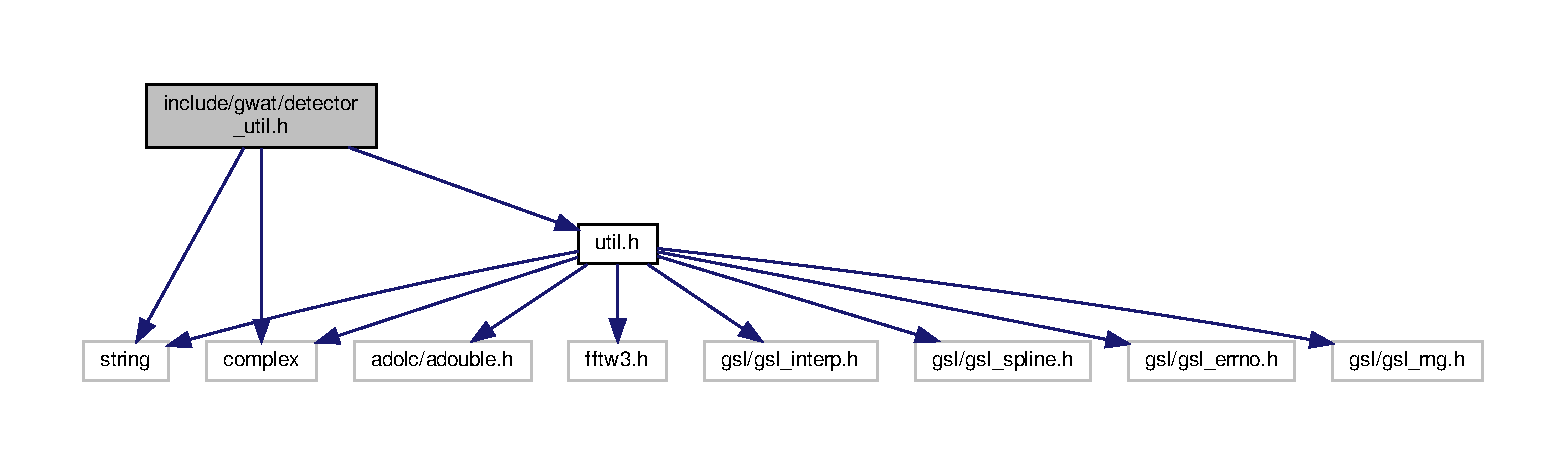
\includegraphics[width=350pt]{detector__util_8h__incl}
\end{center}
\end{figure}
This graph shows which files directly or indirectly include this file\+:\nopagebreak
\begin{figure}[H]
\begin{center}
\leavevmode
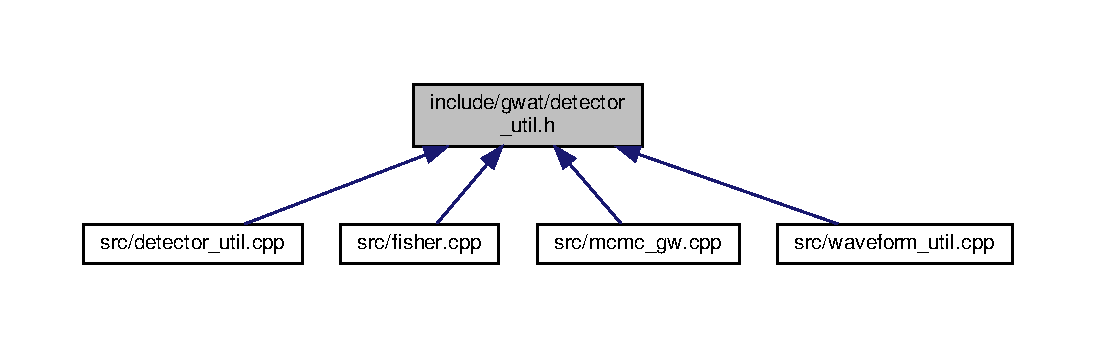
\includegraphics[width=350pt]{detector__util_8h__dep__incl}
\end{center}
\end{figure}
\subsection*{Functions}
\begin{DoxyCompactItemize}
\item 
void \hyperlink{detector__util_8h_a551c603f441283ca3fe5d415d47bdc4d}{populate\+\_\+noise} (double $\ast$frequencies, std\+::string detector, double $\ast$noise\+\_\+root, int length=0)
\item 
void \hyperlink{detector__util_8h_a96e8f667b0106557c0c285dc658b8ac3}{populate\+\_\+noise} (double $\ast$frequencies, std\+::string detector, double $\ast$noise\+\_\+root, int length, double integration\+\_\+time)
\begin{DoxyCompactList}\small\item\em Function to populate the squareroot of the noise curve for various detectors. \end{DoxyCompactList}\item 
double \hyperlink{detector__util_8h_a6e657285283899f91aa3b7ec7963c120}{a\+L\+I\+G\+O\+\_\+analytic} (double f)
\begin{DoxyCompactList}\small\item\em Analytic function approximating the P\+SD for a\+L\+I\+GO. \end{DoxyCompactList}\item 
double \hyperlink{detector__util_8h_a46dad75264f15f490b473cc94ee9b17a}{L\+I\+S\+A\+\_\+analytic\+\_\+\+S\+A\+DC} (double f)
\begin{DoxyCompactList}\small\item\em Analytic function approximating the P\+SD for L\+I\+SA sensitivity curve -- this is S, not root S. \end{DoxyCompactList}\item 
double \hyperlink{detector__util_8h_a6343e73e97f8181b6cfd699c3e92a179}{L\+I\+S\+A\+\_\+analytic} (double f)
\begin{DoxyCompactList}\small\item\em Analytic function approximating the P\+SD for L\+I\+SA sensitivity curve -- this is S, not root S and does not sky average, treats the 2 channels separately, and the geometrical factor of \{3\}/2 is included in the waveform. \end{DoxyCompactList}\item 
double \hyperlink{detector__util_8h_a0c4205a31d277abfd7af6ccb1e6c0ed9}{L\+I\+S\+A\+\_\+\+P\+O\+MS} (double f)
\item 
double \hyperlink{detector__util_8h_a506f9c3f31dd28ea338306b37433fe75}{L\+I\+S\+A\+\_\+\+P\+A\+CC} (double f)
\item 
double \hyperlink{detector__util_8h_abf69df0d2ad243b2ec8fd022164d7d5b}{L\+I\+S\+A\+\_\+\+SC} (double f, double alpha, double beta, double kappa, double gamma, double fk)
\item 
void \hyperlink{detector__util_8h_a47b20a157d8337d411c0d02d0a638168}{sort\+\_\+\+L\+I\+S\+A\+\_\+\+S\+C\+\_\+coeffs} (double $\ast$alpha, double $\ast$beta, double $\ast$kappa, double $\ast$gamma, double $\ast$fk, double integration\+\_\+time)
\item 
std\+::complex$<$ double $>$ \hyperlink{detector__util_8h_a58352b030b231c0a272ad41506a549c5}{Q} (double theta, double phi, double iota)
\begin{DoxyCompactList}\small\item\em Utility for the overall amplitude and phase shift for spin-\/aligned systems. \end{DoxyCompactList}\item 
std\+::complex$<$ double $>$ \hyperlink{detector__util_8h_a9f4ebc828f7a5fdf89f3c3f4243f9288}{Q} (double theta, double phi, double iota, double psi)
\begin{DoxyCompactList}\small\item\em Utility for the overall amplitude and phase shift for spin-\/aligned systems. \end{DoxyCompactList}\item 
{\footnotesize template$<$class T $>$ }\\T \hyperlink{detector__util_8h_a3d3d83c7a398244da315cc9a6f0b15df}{right\+\_\+interferometer\+\_\+cross} (T theta, T phi)
\begin{DoxyCompactList}\small\item\em Response function of a 90 deg interferometer for cross polarization. \end{DoxyCompactList}\item 
{\footnotesize template$<$class T $>$ }\\T \hyperlink{detector__util_8h_aa60bf261e973bd490d1c83015af22aad}{right\+\_\+interferometer\+\_\+plus} (T theta, T phi)
\begin{DoxyCompactList}\small\item\em Response function of a 90 deg interferometer for plus polarization. \end{DoxyCompactList}\item 
{\footnotesize template$<$class T $>$ }\\void \hyperlink{detector__util_8h_a581689a9536c0b115efe2b763e41af17}{right\+\_\+interferometer} (T $\ast$fplus, T $\ast$fcross, T theta, T phi, T psi)
\begin{DoxyCompactList}\small\item\em Response function of a 90 deg interferometer. \end{DoxyCompactList}\item 
double \hyperlink{detector__util_8h_a2e29bfa3018d037af4d1b52cabe47d39}{Hanford\+\_\+\+O1\+\_\+fitted} (double f)
\begin{DoxyCompactList}\small\item\em Numerically fit P\+SD to the Hanford Detector\textquotesingle{}s O1. \end{DoxyCompactList}\item 
{\footnotesize template$<$class T $>$ }\\void \hyperlink{detector__util_8h_af252cb74fb621c53ebe8db50f58841d2}{celestial\+\_\+horizon\+\_\+transform} (T RA, T D\+EC, double gps\+\_\+time, std\+::string detector, T $\ast$phi, T $\ast$theta)
\begin{DoxyCompactList}\small\item\em Transform from celestial coordinates to local horizontal coords. \end{DoxyCompactList}\item 
void \hyperlink{detector__util_8h_a038c7aed643958fb110d2ffa790a854a}{derivative\+\_\+celestial\+\_\+horizon\+\_\+transform} (double RA, double D\+EC, double gps\+\_\+time, std\+::string detector, double $\ast$dphi\+\_\+d\+RA, double $\ast$dtheta\+\_\+d\+RA, double $\ast$dphi\+\_\+d\+D\+EC, double $\ast$dtheta\+\_\+d\+D\+EC)
\begin{DoxyCompactList}\small\item\em Numerical derivative of the transformation. \end{DoxyCompactList}\item 
double \hyperlink{detector__util_8h_a8f5874fbc260906fa9ea664debbe86d4}{D\+T\+OA} (double theta1, double theta2, std\+::string detector1, std\+::string detector2)
\begin{DoxyCompactList}\small\item\em calculate difference in time of arrival (D\+T\+OA) for a given source location and 2 different detectors \end{DoxyCompactList}\item 
double \hyperlink{detector__util_8h_adcb816dfe662ececa657888ff18132bd}{radius\+\_\+at\+\_\+lat} (double latitude, double elevation)
\item 
{\footnotesize template$<$class T $>$ }\\void \hyperlink{detector__util_8h_a321057e1d21ddaf59a77614ec2896a4d}{detector\+\_\+response\+\_\+functions\+\_\+equatorial} (double D\mbox{[}3\mbox{]}\mbox{[}3\mbox{]}, T ra, T dec, T psi, double gmst, T $\ast$Fplus, T $\ast$Fcross)
\begin{DoxyCompactList}\small\item\em Calculates the response coefficients for a detector with response tensor D for a source at RA, Dec, and psi. \end{DoxyCompactList}\item 
{\footnotesize template$<$class T $>$ }\\void \hyperlink{detector__util_8h_a60beec5a8011ff54bb15d8a8c4b0e19f}{detector\+\_\+response\+\_\+functions\+\_\+equatorial} (std\+::string detector, T ra, T dec, T psi, double gmst, T $\ast$Fplus, T $\ast$Fcross)
\begin{DoxyCompactList}\small\item\em Wrapping of the equatorial detector response for terrestial based detectors. \end{DoxyCompactList}\item 
{\footnotesize template$<$class T $>$ }\\void \hyperlink{detector__util_8h_a98735bbb64b36d79ce16b7dfcae9a9aa}{detector\+\_\+response\+\_\+functions\+\_\+equatorial} (std\+::string detector, T ra, T dec, T psi, double gmst, T $\ast$times, int length, T L\+I\+S\+A\+\_\+alpha0, T L\+I\+S\+A\+\_\+phi0, T theta\+\_\+j\+\_\+ecl, T phi\+\_\+j\+\_\+ecl, T $\ast$Fplus, T $\ast$Fcross)
\begin{DoxyCompactList}\small\item\em Same as the other function, but for active and future detectors. \end{DoxyCompactList}\item 
{\footnotesize template$<$class T $>$ }\\T \hyperlink{detector__util_8h_a7de625eb431fcebc15bbdb5469363392}{L\+I\+S\+A\+\_\+response\+\_\+plus\+\_\+time} (T theta\+\_\+s, T phi\+\_\+s, T theta\+\_\+j, T phi\+\_\+j, T alpha\+\_\+0, T phi\+\_\+0, T t)
\begin{DoxyCompactList}\small\item\em Time dependent detector response of L\+I\+SA for non-\/precessing waveforms. \end{DoxyCompactList}\item 
\mbox{\Hypertarget{detector__util_8h_a6fbce1e228adb08be4be970f3ce0afd2}\label{detector__util_8h_a6fbce1e228adb08be4be970f3ce0afd2}} 
{\footnotesize template$<$class T $>$ }\\T {\bfseries L\+I\+S\+A\+\_\+response\+\_\+cross\+\_\+time} (T theta\+\_\+s, T phi\+\_\+s, T theta\+\_\+j, T phi\+\_\+j, T alpha\+\_\+0, T phi\+\_\+0, T t)
\item 
\mbox{\Hypertarget{detector__util_8h_aa1d967791d721cd8bd22be0c34066267}\label{detector__util_8h_aa1d967791d721cd8bd22be0c34066267}} 
{\footnotesize template$<$class T $>$ }\\T {\bfseries L\+I\+S\+A\+\_\+response\+\_\+plus} (\hyperlink{structsource__parameters}{source\+\_\+parameters}$<$ T $>$ $\ast$params, T theta\+\_\+s, T phi\+\_\+s, T theta\+\_\+j, T phi\+\_\+j, T alpha\+\_\+0, T phi\+\_\+0, T f)
\item 
\mbox{\Hypertarget{detector__util_8h_a8518f8bcc6de5339871bbd4881579654}\label{detector__util_8h_a8518f8bcc6de5339871bbd4881579654}} 
{\footnotesize template$<$class T $>$ }\\T {\bfseries L\+I\+S\+A\+\_\+response\+\_\+cross} (\hyperlink{structsource__parameters}{source\+\_\+parameters}$<$ T $>$ $\ast$params, T theta\+\_\+s, T phi\+\_\+s, T theta\+\_\+j, T phi\+\_\+j, T alpha\+\_\+0, T phi\+\_\+0, T f)
\item 
double \hyperlink{detector__util_8h_a742264b5eeff1d244e299d47cb7fa084}{p\+\_\+single\+\_\+detector} (double omega, int samples)
\begin{DoxyCompactList}\small\item\em Utility to calculate the cumulative amplitude distribution for a single detector. \end{DoxyCompactList}\item 
double \hyperlink{detector__util_8h_a0af90e8d6505794a792d2b35bf583bef}{p\+\_\+single\+\_\+detector\+\_\+fit} (double omega)
\begin{DoxyCompactList}\small\item\em Utility to calculate the cumulative amplitude distribution for a single detector -- Numerical Fit. \end{DoxyCompactList}\item 
double \hyperlink{detector__util_8h_a8470b24a84da4e746ee95ff9bb87bbbc}{p\+\_\+triple\+\_\+detector\+\_\+fit} (double omega)
\begin{DoxyCompactList}\small\item\em Utility to calculate the cumulative amplitude distribution for triple detector network -- Numerical Fit. \end{DoxyCompactList}\item 
\mbox{\Hypertarget{detector__util_8h_a844b28c8dcc0fcbb014b38c1ba013811}\label{detector__util_8h_a844b28c8dcc0fcbb014b38c1ba013811}} 
double {\bfseries pdet\+\_\+triple\+\_\+detector\+\_\+fit} (double rho\+\_\+thresh, double rho\+\_\+opt)
\item 
double \hyperlink{detector__util_8h_a2806107bf836833162b1f7e2b78b14d5}{p\+\_\+triple\+\_\+detector\+\_\+interp} (double omega)
\begin{DoxyCompactList}\small\item\em Utility to calculate the cumulative amplitude distribution for triple detector network -- interpolated data from \href{https://pages.jh.edu/~eberti2/research/}{\tt https\+://pages.\+jh.\+edu/$\sim$eberti2/research/}. \end{DoxyCompactList}\item 
double \hyperlink{detector__util_8h_a38cf74dd41080e18fc64000605019c50}{p\+\_\+single\+\_\+detector\+\_\+interp} (double omega)
\begin{DoxyCompactList}\small\item\em Utility to calculate the cumulative amplitude distribution for single detector network -- interpolated data from \href{https://pages.jh.edu/~eberti2/research/}{\tt https\+://pages.\+jh.\+edu/$\sim$eberti2/research/}. \end{DoxyCompactList}\end{DoxyCompactItemize}
\subsection*{Variables}
\begin{DoxyCompactItemize}
\item 
\mbox{\Hypertarget{detector__util_8h_a1cd39022a1e102835a1ac1b513b61426}\label{detector__util_8h_a1cd39022a1e102835a1ac1b513b61426}} 
const double {\bfseries H\+\_\+\+L\+AT} =0.\+81079526383
\item 
\mbox{\Hypertarget{detector__util_8h_ad71c7f7f5ecd2c0c4e72a476b60f9761}\label{detector__util_8h_ad71c7f7f5ecd2c0c4e72a476b60f9761}} 
const double {\bfseries H\+\_\+\+L\+O\+NG} =-\/2.\+08405676917
\item 
\mbox{\Hypertarget{detector__util_8h_afdd407ebec95f17b9aabe05a3a22c433}\label{detector__util_8h_afdd407ebec95f17b9aabe05a3a22c433}} 
const double {\bfseries H\+\_\+azimuth\+\_\+offset} = 2.\+199
\item 
\mbox{\Hypertarget{detector__util_8h_a000abb0905c1fd62ad0484a9adada609}\label{detector__util_8h_a000abb0905c1fd62ad0484a9adada609}} 
const double {\bfseries H\+\_\+radius} = 6367299.\+93401105
\item 
\mbox{\Hypertarget{detector__util_8h_a884237ad810a64b6f36e5554cc956158}\label{detector__util_8h_a884237ad810a64b6f36e5554cc956158}} 
const double {\bfseries H\+\_\+elevation} = 142.\+554
\item 
\mbox{\Hypertarget{detector__util_8h_a97ab81c0ffd5094dd9b6aab103b9fe28}\label{detector__util_8h_a97ab81c0ffd5094dd9b6aab103b9fe28}} 
const double {\bfseries L\+\_\+\+L\+AT} =0.\+53342313506
\item 
\mbox{\Hypertarget{detector__util_8h_a25dd7af0706792ee46f31f722cf7a088}\label{detector__util_8h_a25dd7af0706792ee46f31f722cf7a088}} 
const double {\bfseries L\+\_\+\+L\+O\+NG} =-\/1.\+58430937078
\item 
\mbox{\Hypertarget{detector__util_8h_a79cd8bb6223213a2f531e5f0ade75722}\label{detector__util_8h_a79cd8bb6223213a2f531e5f0ade75722}} 
const double {\bfseries L\+\_\+azimuth\+\_\+offset} = 3.\+4557
\item 
\mbox{\Hypertarget{detector__util_8h_a2ecb143a4eba4acce843ea917892c614}\label{detector__util_8h_a2ecb143a4eba4acce843ea917892c614}} 
const double {\bfseries L\+\_\+radius} = 6372795.\+50144497
\item 
\mbox{\Hypertarget{detector__util_8h_afdbdb8fbcc95c979b35ae51f325b2925}\label{detector__util_8h_afdbdb8fbcc95c979b35ae51f325b2925}} 
const double {\bfseries L\+\_\+elevation} = -\/6.\+574
\item 
\mbox{\Hypertarget{detector__util_8h_af746e081b047e8905f5593b65f4487d4}\label{detector__util_8h_af746e081b047e8905f5593b65f4487d4}} 
const double {\bfseries V\+\_\+\+L\+AT} =0.\+76151183984
\item 
\mbox{\Hypertarget{detector__util_8h_a032dccbec455c3e9f987df873fe06fed}\label{detector__util_8h_a032dccbec455c3e9f987df873fe06fed}} 
const double {\bfseries V\+\_\+\+L\+O\+NG} =0.\+18333805213
\item 
\mbox{\Hypertarget{detector__util_8h_a16f6c7a9877eebfc2197e0d250a6f5bc}\label{detector__util_8h_a16f6c7a9877eebfc2197e0d250a6f5bc}} 
const double {\bfseries V\+\_\+azimuth\+\_\+offset} = 1.\+239
\item 
\mbox{\Hypertarget{detector__util_8h_afe6dc4a785ca00eb42fcb21abdad9121}\label{detector__util_8h_afe6dc4a785ca00eb42fcb21abdad9121}} 
const double {\bfseries V\+\_\+radius} = 6368051.\+92301
\item 
\mbox{\Hypertarget{detector__util_8h_a5644ef4e7c76e45807a0b6219b7f6037}\label{detector__util_8h_a5644ef4e7c76e45807a0b6219b7f6037}} 
const double {\bfseries V\+\_\+elevation} = 51.\+884
\item 
\mbox{\Hypertarget{detector__util_8h_a2cd979387f9d48def1737eb3af260e89}\label{detector__util_8h_a2cd979387f9d48def1737eb3af260e89}} 
const double {\bfseries R\+E\+\_\+polar} =6357e3
\item 
\mbox{\Hypertarget{detector__util_8h_a2e6b415e67d67ab0ef09f0f8fec532ad}\label{detector__util_8h_a2e6b415e67d67ab0ef09f0f8fec532ad}} 
const double {\bfseries R\+E\+\_\+equatorial} = 6378e3
\item 
const double \hyperlink{detector__util_8h_a14eced5d747f703b86f021cfc242536e}{Hanford\+\_\+D} \mbox{[}3\mbox{]}\mbox{[}3\mbox{]}
\item 
const double \hyperlink{detector__util_8h_ac5616b73b3ed3913e803bc76573677aa}{Livingston\+\_\+D} \mbox{[}3\mbox{]}\mbox{[}3\mbox{]}
\item 
const double \hyperlink{detector__util_8h_ab3f9eb7bf2b7778fd56ed0a48ddaf423}{Virgo\+\_\+D} \mbox{[}3\mbox{]}\mbox{[}3\mbox{]}
\end{DoxyCompactItemize}


\subsection{Detailed Description}
Header file for all detector-\/specific utilities 

\subsection{Function Documentation}
\mbox{\Hypertarget{detector__util_8h_a6e657285283899f91aa3b7ec7963c120}\label{detector__util_8h_a6e657285283899f91aa3b7ec7963c120}} 
\index{detector\+\_\+util.\+h@{detector\+\_\+util.\+h}!a\+L\+I\+G\+O\+\_\+analytic@{a\+L\+I\+G\+O\+\_\+analytic}}
\index{a\+L\+I\+G\+O\+\_\+analytic@{a\+L\+I\+G\+O\+\_\+analytic}!detector\+\_\+util.\+h@{detector\+\_\+util.\+h}}
\subsubsection{\texorpdfstring{a\+L\+I\+G\+O\+\_\+analytic()}{aLIGO\_analytic()}}
{\footnotesize\ttfamily double a\+L\+I\+G\+O\+\_\+analytic (\begin{DoxyParamCaption}\item[{double}]{f }\end{DoxyParamCaption})}



Analytic function approximating the P\+SD for a\+L\+I\+GO. 

C\+I\+TE (Will?) \mbox{\Hypertarget{detector__util_8h_af252cb74fb621c53ebe8db50f58841d2}\label{detector__util_8h_af252cb74fb621c53ebe8db50f58841d2}} 
\index{detector\+\_\+util.\+h@{detector\+\_\+util.\+h}!celestial\+\_\+horizon\+\_\+transform@{celestial\+\_\+horizon\+\_\+transform}}
\index{celestial\+\_\+horizon\+\_\+transform@{celestial\+\_\+horizon\+\_\+transform}!detector\+\_\+util.\+h@{detector\+\_\+util.\+h}}
\subsubsection{\texorpdfstring{celestial\+\_\+horizon\+\_\+transform()}{celestial\_horizon\_transform()}}
{\footnotesize\ttfamily template$<$class T $>$ \\
void celestial\+\_\+horizon\+\_\+transform (\begin{DoxyParamCaption}\item[{T}]{RA,  }\item[{T}]{D\+EC,  }\item[{double}]{gps\+\_\+time,  }\item[{std\+::string}]{detector,  }\item[{T $\ast$}]{phi,  }\item[{T $\ast$}]{theta }\end{DoxyParamCaption})}



Transform from celestial coordinates to local horizontal coords. 

(RA,D\+EC) -\/$>$ (altitude, azimuth)

Need gps\+\_\+time of transformation, as the horizontal coords change in time

detector is used to specify the lat and long of the local frame 
\begin{DoxyParams}{Parameters}
{\em RA} & in R\+AD \\
\hline
{\em D\+EC} & in R\+AD \\
\hline
{\em phi} & in R\+AD \\
\hline
{\em theta} & in R\+AD \\
\hline
\end{DoxyParams}
\mbox{\Hypertarget{detector__util_8h_a038c7aed643958fb110d2ffa790a854a}\label{detector__util_8h_a038c7aed643958fb110d2ffa790a854a}} 
\index{detector\+\_\+util.\+h@{detector\+\_\+util.\+h}!derivative\+\_\+celestial\+\_\+horizon\+\_\+transform@{derivative\+\_\+celestial\+\_\+horizon\+\_\+transform}}
\index{derivative\+\_\+celestial\+\_\+horizon\+\_\+transform@{derivative\+\_\+celestial\+\_\+horizon\+\_\+transform}!detector\+\_\+util.\+h@{detector\+\_\+util.\+h}}
\subsubsection{\texorpdfstring{derivative\+\_\+celestial\+\_\+horizon\+\_\+transform()}{derivative\_celestial\_horizon\_transform()}}
{\footnotesize\ttfamily void derivative\+\_\+celestial\+\_\+horizon\+\_\+transform (\begin{DoxyParamCaption}\item[{double}]{RA,  }\item[{double}]{D\+EC,  }\item[{double}]{gps\+\_\+time,  }\item[{std\+::string}]{detector,  }\item[{double $\ast$}]{dphi\+\_\+d\+RA,  }\item[{double $\ast$}]{dtheta\+\_\+d\+RA,  }\item[{double $\ast$}]{dphi\+\_\+d\+D\+EC,  }\item[{double $\ast$}]{dtheta\+\_\+d\+D\+EC }\end{DoxyParamCaption})}



Numerical derivative of the transformation. 

Planned for use in Fisher calculations, but not currently implemented anywhere 
\begin{DoxyParams}{Parameters}
{\em RA} & in R\+AD \\
\hline
{\em D\+EC} & in R\+AD \\
\hline
\end{DoxyParams}
\mbox{\Hypertarget{detector__util_8h_a321057e1d21ddaf59a77614ec2896a4d}\label{detector__util_8h_a321057e1d21ddaf59a77614ec2896a4d}} 
\index{detector\+\_\+util.\+h@{detector\+\_\+util.\+h}!detector\+\_\+response\+\_\+functions\+\_\+equatorial@{detector\+\_\+response\+\_\+functions\+\_\+equatorial}}
\index{detector\+\_\+response\+\_\+functions\+\_\+equatorial@{detector\+\_\+response\+\_\+functions\+\_\+equatorial}!detector\+\_\+util.\+h@{detector\+\_\+util.\+h}}
\subsubsection{\texorpdfstring{detector\+\_\+response\+\_\+functions\+\_\+equatorial()}{detector\_response\_functions\_equatorial()}\hspace{0.1cm}{\footnotesize\ttfamily [1/3]}}
{\footnotesize\ttfamily template$<$class T $>$ \\
void detector\+\_\+response\+\_\+functions\+\_\+equatorial (\begin{DoxyParamCaption}\item[{double}]{D\mbox{[}3\mbox{]}\mbox{[}3\mbox{]},  }\item[{T}]{ra,  }\item[{T}]{dec,  }\item[{T}]{psi,  }\item[{double}]{gmst,  }\item[{T $\ast$}]{Fplus,  }\item[{T $\ast$}]{Fcross }\end{DoxyParamCaption})}



Calculates the response coefficients for a detector with response tensor D for a source at RA, Dec, and psi. 

Taken from L\+A\+L\+Suite

The response tensor for each of the operational detectors is precomputed in \hyperlink{detector__util_8h}{detector\+\_\+util.\+h}, but to create a new tensor, follow the outline in Anderson et al 36 P\+RD 63 042003 (2001) Appendix B

For terrestial detectors -- psi is the polarization angle from a detector at earth\textquotesingle{}s center, aligned with equatorial coordinates 
\begin{DoxyParams}[1]{Parameters}
 & {\em D} & Detector Response tensor (3x3) \\
\hline
 & {\em ra} & Right ascension in rad \\
\hline
 & {\em dec} & Declination in rad \\
\hline
 & {\em psi} & polarization angle in rad \\
\hline
 & {\em gmst} & Greenwich mean sidereal time (rad) \\
\hline
\mbox{\tt out}  & {\em Fplus} & Fplus response coefficient \\
\hline
\mbox{\tt out}  & {\em Fcross} & Fcross response coefficient \\
\hline
\end{DoxyParams}
\mbox{\Hypertarget{detector__util_8h_a60beec5a8011ff54bb15d8a8c4b0e19f}\label{detector__util_8h_a60beec5a8011ff54bb15d8a8c4b0e19f}} 
\index{detector\+\_\+util.\+h@{detector\+\_\+util.\+h}!detector\+\_\+response\+\_\+functions\+\_\+equatorial@{detector\+\_\+response\+\_\+functions\+\_\+equatorial}}
\index{detector\+\_\+response\+\_\+functions\+\_\+equatorial@{detector\+\_\+response\+\_\+functions\+\_\+equatorial}!detector\+\_\+util.\+h@{detector\+\_\+util.\+h}}
\subsubsection{\texorpdfstring{detector\+\_\+response\+\_\+functions\+\_\+equatorial()}{detector\_response\_functions\_equatorial()}\hspace{0.1cm}{\footnotesize\ttfamily [2/3]}}
{\footnotesize\ttfamily template$<$class T $>$ \\
void detector\+\_\+response\+\_\+functions\+\_\+equatorial (\begin{DoxyParamCaption}\item[{std\+::string}]{detector,  }\item[{T}]{ra,  }\item[{T}]{dec,  }\item[{T}]{psi,  }\item[{double}]{gmst,  }\item[{T $\ast$}]{Fplus,  }\item[{T $\ast$}]{Fcross }\end{DoxyParamCaption})}



Wrapping of the equatorial detector response for terrestial based detectors. 

For ground based detectors, the antenna pattern functions are not functions of time. 
\begin{DoxyParams}[1]{Parameters}
 & {\em detector} & Detector \\
\hline
 & {\em ra} & Right ascension in rad \\
\hline
 & {\em dec} & Declination in rad \\
\hline
 & {\em psi} & polarization angle in rad \\
\hline
 & {\em gmst} & Greenwich mean sidereal time (rad) \\
\hline
\mbox{\tt out}  & {\em Fplus} & Fplus response coefficient \\
\hline
\mbox{\tt out}  & {\em Fcross} & Fcross response coefficient \\
\hline
\end{DoxyParams}
\mbox{\Hypertarget{detector__util_8h_a98735bbb64b36d79ce16b7dfcae9a9aa}\label{detector__util_8h_a98735bbb64b36d79ce16b7dfcae9a9aa}} 
\index{detector\+\_\+util.\+h@{detector\+\_\+util.\+h}!detector\+\_\+response\+\_\+functions\+\_\+equatorial@{detector\+\_\+response\+\_\+functions\+\_\+equatorial}}
\index{detector\+\_\+response\+\_\+functions\+\_\+equatorial@{detector\+\_\+response\+\_\+functions\+\_\+equatorial}!detector\+\_\+util.\+h@{detector\+\_\+util.\+h}}
\subsubsection{\texorpdfstring{detector\+\_\+response\+\_\+functions\+\_\+equatorial()}{detector\_response\_functions\_equatorial()}\hspace{0.1cm}{\footnotesize\ttfamily [3/3]}}
{\footnotesize\ttfamily template$<$class T $>$ \\
void detector\+\_\+response\+\_\+functions\+\_\+equatorial (\begin{DoxyParamCaption}\item[{std\+::string}]{detector,  }\item[{T}]{ra,  }\item[{T}]{dec,  }\item[{T}]{psi,  }\item[{double}]{gmst,  }\item[{T $\ast$}]{times,  }\item[{int}]{length,  }\item[{T}]{L\+I\+S\+A\+\_\+alpha0,  }\item[{T}]{L\+I\+S\+A\+\_\+phi0,  }\item[{T}]{theta\+\_\+j\+\_\+ecl,  }\item[{T}]{phi\+\_\+j\+\_\+ecl,  }\item[{T $\ast$}]{Fplus,  }\item[{T $\ast$}]{Fcross }\end{DoxyParamCaption})}



Same as the other function, but for active and future detectors. 

If terrestial detectors, it will use ra, dec, psi, and gmst

If space detector, it will use ra, dec transformed to ecliptic coord, and L\+I\+S\+A\+\_\+alpha0, L\+I\+S\+A\+\_\+phi0 and theta\+\_\+j\+\_\+ecl, phi\+\_\+j\+\_\+ecl, which are the offsets for L\+I\+SA and the spherical angles for the unit vector in the total angular momemntum in the ecliptic system 
\begin{DoxyParams}[1]{Parameters}
 & {\em detector} & Detector \\
\hline
 & {\em ra} & Right ascension in rad \\
\hline
 & {\em dec} & Declination in rad \\
\hline
 & {\em psi} & polarization angle in rad \\
\hline
 & {\em gmst} & Greenwich mean sidereal time (rad) \\
\hline
 & {\em times} & Times at which to evaluate Fplus and Fcross, in which case the Fplus and Fcross pointers are arrays \\
\hline
 & {\em length} & Length of the arrays \\
\hline
 & {\em L\+I\+S\+A\+\_\+alpha0} & Offset for alpha \\
\hline
 & {\em L\+I\+S\+A\+\_\+phi0} & Offset for phi \\
\hline
 & {\em theta\+\_\+j\+\_\+ecl} & Ecliptic spherical polar angle of Lhat (Jhat for precessing systems) \\
\hline
 & {\em phi\+\_\+j\+\_\+ecl} & Ecliptic sherical azimuthal angle (Jhat for precessing systems) \\
\hline
\mbox{\tt out}  & {\em Fplus} & Fplus response coefficient \\
\hline
\mbox{\tt out}  & {\em Fcross} & Fcross response coefficient \\
\hline
\end{DoxyParams}
\mbox{\Hypertarget{detector__util_8h_a8f5874fbc260906fa9ea664debbe86d4}\label{detector__util_8h_a8f5874fbc260906fa9ea664debbe86d4}} 
\index{detector\+\_\+util.\+h@{detector\+\_\+util.\+h}!D\+T\+OA@{D\+T\+OA}}
\index{D\+T\+OA@{D\+T\+OA}!detector\+\_\+util.\+h@{detector\+\_\+util.\+h}}
\subsubsection{\texorpdfstring{D\+T\+O\+A()}{DTOA()}}
{\footnotesize\ttfamily double D\+T\+OA (\begin{DoxyParamCaption}\item[{double}]{theta1,  }\item[{double}]{theta2,  }\item[{std\+::string}]{detector1,  }\item[{std\+::string}]{detector2 }\end{DoxyParamCaption})}



calculate difference in time of arrival (D\+T\+OA) for a given source location and 2 different detectors 


\begin{DoxyParams}{Parameters}
{\em theta1} & spherical polar angle for detector 1 in R\+AD \\
\hline
{\em theta2} & spherical polar angle for detector 2 in R\+AD \\
\hline
{\em detector1} & name of detector one \\
\hline
{\em detector2} & name of detector two \\
\hline
\end{DoxyParams}
\mbox{\Hypertarget{detector__util_8h_a2e29bfa3018d037af4d1b52cabe47d39}\label{detector__util_8h_a2e29bfa3018d037af4d1b52cabe47d39}} 
\index{detector\+\_\+util.\+h@{detector\+\_\+util.\+h}!Hanford\+\_\+\+O1\+\_\+fitted@{Hanford\+\_\+\+O1\+\_\+fitted}}
\index{Hanford\+\_\+\+O1\+\_\+fitted@{Hanford\+\_\+\+O1\+\_\+fitted}!detector\+\_\+util.\+h@{detector\+\_\+util.\+h}}
\subsubsection{\texorpdfstring{Hanford\+\_\+\+O1\+\_\+fitted()}{Hanford\_O1\_fitted()}}
{\footnotesize\ttfamily double Hanford\+\_\+\+O1\+\_\+fitted (\begin{DoxyParamCaption}\item[{double}]{f }\end{DoxyParamCaption})}



Numerically fit P\+SD to the Hanford Detector\textquotesingle{}s O1. 

C\+I\+TE (Yunes?) \mbox{\Hypertarget{detector__util_8h_a6343e73e97f8181b6cfd699c3e92a179}\label{detector__util_8h_a6343e73e97f8181b6cfd699c3e92a179}} 
\index{detector\+\_\+util.\+h@{detector\+\_\+util.\+h}!L\+I\+S\+A\+\_\+analytic@{L\+I\+S\+A\+\_\+analytic}}
\index{L\+I\+S\+A\+\_\+analytic@{L\+I\+S\+A\+\_\+analytic}!detector\+\_\+util.\+h@{detector\+\_\+util.\+h}}
\subsubsection{\texorpdfstring{L\+I\+S\+A\+\_\+analytic()}{LISA\_analytic()}}
{\footnotesize\ttfamily double L\+I\+S\+A\+\_\+analytic (\begin{DoxyParamCaption}\item[{double}]{f }\end{DoxyParamCaption})}



Analytic function approximating the P\+SD for L\+I\+SA sensitivity curve -- this is S, not root S and does not sky average, treats the 2 channels separately, and the geometrical factor of \{3\}/2 is included in the waveform. 

N\+ON Sky averaged -\/ single channel

ar\+Xiv\+:1905.\+08811 -- equation 14-\/17 \mbox{\Hypertarget{detector__util_8h_a46dad75264f15f490b473cc94ee9b17a}\label{detector__util_8h_a46dad75264f15f490b473cc94ee9b17a}} 
\index{detector\+\_\+util.\+h@{detector\+\_\+util.\+h}!L\+I\+S\+A\+\_\+analytic\+\_\+\+S\+A\+DC@{L\+I\+S\+A\+\_\+analytic\+\_\+\+S\+A\+DC}}
\index{L\+I\+S\+A\+\_\+analytic\+\_\+\+S\+A\+DC@{L\+I\+S\+A\+\_\+analytic\+\_\+\+S\+A\+DC}!detector\+\_\+util.\+h@{detector\+\_\+util.\+h}}
\subsubsection{\texorpdfstring{L\+I\+S\+A\+\_\+analytic\+\_\+\+S\+A\+D\+C()}{LISA\_analytic\_SADC()}}
{\footnotesize\ttfamily double L\+I\+S\+A\+\_\+analytic\+\_\+\+S\+A\+DC (\begin{DoxyParamCaption}\item[{double}]{f }\end{DoxyParamCaption})}



Analytic function approximating the P\+SD for L\+I\+SA sensitivity curve -- this is S, not root S. 

Sky averaged -\/ dual channel

ar\+Xiv\+:1803.\+01944 -- equation 13

N\+O\+TE\+: may need to divide by \{3\}/2.. My L\+I\+SA response functions already include this factor -- factor 0f 3./4. (sqrt(3)/2)$\ast$$\ast$2

Keeping the factor of sqrt(3)/2, since this will probably be used without the beam patter functions (that\textquotesingle{}s where the factor of sqrt(3)/2 usually appears) \mbox{\Hypertarget{detector__util_8h_a506f9c3f31dd28ea338306b37433fe75}\label{detector__util_8h_a506f9c3f31dd28ea338306b37433fe75}} 
\index{detector\+\_\+util.\+h@{detector\+\_\+util.\+h}!L\+I\+S\+A\+\_\+\+P\+A\+CC@{L\+I\+S\+A\+\_\+\+P\+A\+CC}}
\index{L\+I\+S\+A\+\_\+\+P\+A\+CC@{L\+I\+S\+A\+\_\+\+P\+A\+CC}!detector\+\_\+util.\+h@{detector\+\_\+util.\+h}}
\subsubsection{\texorpdfstring{L\+I\+S\+A\+\_\+\+P\+A\+C\+C()}{LISA\_PACC()}}
{\footnotesize\ttfamily double L\+I\+S\+A\+\_\+\+P\+A\+CC (\begin{DoxyParamCaption}\item[{double}]{f }\end{DoxyParamCaption})}

Single test mass accelartion noise

ar\+Xiv\+:1803.\+01944 -- equation 11 \mbox{\Hypertarget{detector__util_8h_a0c4205a31d277abfd7af6ccb1e6c0ed9}\label{detector__util_8h_a0c4205a31d277abfd7af6ccb1e6c0ed9}} 
\index{detector\+\_\+util.\+h@{detector\+\_\+util.\+h}!L\+I\+S\+A\+\_\+\+P\+O\+MS@{L\+I\+S\+A\+\_\+\+P\+O\+MS}}
\index{L\+I\+S\+A\+\_\+\+P\+O\+MS@{L\+I\+S\+A\+\_\+\+P\+O\+MS}!detector\+\_\+util.\+h@{detector\+\_\+util.\+h}}
\subsubsection{\texorpdfstring{L\+I\+S\+A\+\_\+\+P\+O\+M\+S()}{LISA\_POMS()}}
{\footnotesize\ttfamily double L\+I\+S\+A\+\_\+\+P\+O\+MS (\begin{DoxyParamCaption}\item[{double}]{f }\end{DoxyParamCaption})}

Optical metrology noise function

ar\+Xiv\+:1803.\+01944 -- equation 10 \mbox{\Hypertarget{detector__util_8h_a7de625eb431fcebc15bbdb5469363392}\label{detector__util_8h_a7de625eb431fcebc15bbdb5469363392}} 
\index{detector\+\_\+util.\+h@{detector\+\_\+util.\+h}!L\+I\+S\+A\+\_\+response\+\_\+plus\+\_\+time@{L\+I\+S\+A\+\_\+response\+\_\+plus\+\_\+time}}
\index{L\+I\+S\+A\+\_\+response\+\_\+plus\+\_\+time@{L\+I\+S\+A\+\_\+response\+\_\+plus\+\_\+time}!detector\+\_\+util.\+h@{detector\+\_\+util.\+h}}
\subsubsection{\texorpdfstring{L\+I\+S\+A\+\_\+response\+\_\+plus\+\_\+time()}{LISA\_response\_plus\_time()}}
{\footnotesize\ttfamily template$<$class T $>$ \\
T L\+I\+S\+A\+\_\+response\+\_\+plus\+\_\+time (\begin{DoxyParamCaption}\item[{T}]{theta\+\_\+s,  }\item[{T}]{phi\+\_\+s,  }\item[{T}]{theta\+\_\+j,  }\item[{T}]{phi\+\_\+j,  }\item[{T}]{alpha\+\_\+0,  }\item[{T}]{phi\+\_\+0,  }\item[{T}]{t }\end{DoxyParamCaption})}



Time dependent detector response of L\+I\+SA for non-\/precessing waveforms. 

See \href{https://arxiv.org/abs/gr-qc/0411129}{\tt https\+://arxiv.\+org/abs/gr-\/qc/0411129} or \href{https://arxiv.org/abs/gr-qc/9703068}{\tt https\+://arxiv.\+org/abs/gr-\/qc/9703068}

All the arguments are ``barred\textquotesingle{}\textquotesingle{}, using the notation in these two works. That is, they are relative to the solar system barycenter.

To get the second interferometer\textquotesingle{}s response, evaluate with phi\+\_\+j -\/ pi/4.

All the coordinates are in the ecliptic coordinate system \mbox{\Hypertarget{detector__util_8h_abf69df0d2ad243b2ec8fd022164d7d5b}\label{detector__util_8h_abf69df0d2ad243b2ec8fd022164d7d5b}} 
\index{detector\+\_\+util.\+h@{detector\+\_\+util.\+h}!L\+I\+S\+A\+\_\+\+SC@{L\+I\+S\+A\+\_\+\+SC}}
\index{L\+I\+S\+A\+\_\+\+SC@{L\+I\+S\+A\+\_\+\+SC}!detector\+\_\+util.\+h@{detector\+\_\+util.\+h}}
\subsubsection{\texorpdfstring{L\+I\+S\+A\+\_\+\+S\+C()}{LISA\_SC()}}
{\footnotesize\ttfamily double L\+I\+S\+A\+\_\+\+SC (\begin{DoxyParamCaption}\item[{double}]{f,  }\item[{double}]{alpha,  }\item[{double}]{beta,  }\item[{double}]{kappa,  }\item[{double}]{gamma,  }\item[{double}]{fk }\end{DoxyParamCaption})}

Confusion noise -- this is S, not root S

ar\+Xiv\+:1803.\+01944 -- 14

integration\+\_\+time is the observation time in months -- options are 6, 12, 24, and 48 \mbox{\Hypertarget{detector__util_8h_a742264b5eeff1d244e299d47cb7fa084}\label{detector__util_8h_a742264b5eeff1d244e299d47cb7fa084}} 
\index{detector\+\_\+util.\+h@{detector\+\_\+util.\+h}!p\+\_\+single\+\_\+detector@{p\+\_\+single\+\_\+detector}}
\index{p\+\_\+single\+\_\+detector@{p\+\_\+single\+\_\+detector}!detector\+\_\+util.\+h@{detector\+\_\+util.\+h}}
\subsubsection{\texorpdfstring{p\+\_\+single\+\_\+detector()}{p\_single\_detector()}}
{\footnotesize\ttfamily double p\+\_\+single\+\_\+detector (\begin{DoxyParamCaption}\item[{double}]{omega,  }\item[{int}]{samples }\end{DoxyParamCaption})}



Utility to calculate the cumulative amplitude distribution for a single detector. 

P() =  (\textquotesingle{}(, , )-\/) d d dcos

Integrated over the volume which \textquotesingle{} is larger than 

Integrates using Monte Carlo integration

Uniform sampling in , cos(), cos() , and  
\begin{DoxyParams}{Parameters}
{\em omega} & = /$\ast$ \\
\hline
{\em samples} & number of monte carlo samples to use$\ast$ \\
\hline
\end{DoxyParams}
\mbox{\Hypertarget{detector__util_8h_a0af90e8d6505794a792d2b35bf583bef}\label{detector__util_8h_a0af90e8d6505794a792d2b35bf583bef}} 
\index{detector\+\_\+util.\+h@{detector\+\_\+util.\+h}!p\+\_\+single\+\_\+detector\+\_\+fit@{p\+\_\+single\+\_\+detector\+\_\+fit}}
\index{p\+\_\+single\+\_\+detector\+\_\+fit@{p\+\_\+single\+\_\+detector\+\_\+fit}!detector\+\_\+util.\+h@{detector\+\_\+util.\+h}}
\subsubsection{\texorpdfstring{p\+\_\+single\+\_\+detector\+\_\+fit()}{p\_single\_detector\_fit()}}
{\footnotesize\ttfamily double p\+\_\+single\+\_\+detector\+\_\+fit (\begin{DoxyParamCaption}\item[{double}]{omega }\end{DoxyParamCaption})}



Utility to calculate the cumulative amplitude distribution for a single detector -- Numerical Fit. 

P() =  (\textquotesingle{}(, , )-\/) d d dcos

Integrated over the volume which \textquotesingle{} is larger than 

see ar\+Xiv\+:1405.\+7016 
\begin{DoxyParams}{Parameters}
{\em omega} & = /$\ast$ \\
\hline
\end{DoxyParams}
\mbox{\Hypertarget{detector__util_8h_a38cf74dd41080e18fc64000605019c50}\label{detector__util_8h_a38cf74dd41080e18fc64000605019c50}} 
\index{detector\+\_\+util.\+h@{detector\+\_\+util.\+h}!p\+\_\+single\+\_\+detector\+\_\+interp@{p\+\_\+single\+\_\+detector\+\_\+interp}}
\index{p\+\_\+single\+\_\+detector\+\_\+interp@{p\+\_\+single\+\_\+detector\+\_\+interp}!detector\+\_\+util.\+h@{detector\+\_\+util.\+h}}
\subsubsection{\texorpdfstring{p\+\_\+single\+\_\+detector\+\_\+interp()}{p\_single\_detector\_interp()}}
{\footnotesize\ttfamily double p\+\_\+single\+\_\+detector\+\_\+interp (\begin{DoxyParamCaption}\item[{double}]{omega }\end{DoxyParamCaption})}



Utility to calculate the cumulative amplitude distribution for single detector network -- interpolated data from \href{https://pages.jh.edu/~eberti2/research/}{\tt https\+://pages.\+jh.\+edu/$\sim$eberti2/research/}. 

P() =  (\textquotesingle{}(, , )-\/) d d dcos

Integrated over the volume which \textquotesingle{} is larger than 

see ar\+Xiv\+:1405.\+7016 
\begin{DoxyParams}{Parameters}
{\em omega} & = /$\ast$ \\
\hline
\end{DoxyParams}
\mbox{\Hypertarget{detector__util_8h_a8470b24a84da4e746ee95ff9bb87bbbc}\label{detector__util_8h_a8470b24a84da4e746ee95ff9bb87bbbc}} 
\index{detector\+\_\+util.\+h@{detector\+\_\+util.\+h}!p\+\_\+triple\+\_\+detector\+\_\+fit@{p\+\_\+triple\+\_\+detector\+\_\+fit}}
\index{p\+\_\+triple\+\_\+detector\+\_\+fit@{p\+\_\+triple\+\_\+detector\+\_\+fit}!detector\+\_\+util.\+h@{detector\+\_\+util.\+h}}
\subsubsection{\texorpdfstring{p\+\_\+triple\+\_\+detector\+\_\+fit()}{p\_triple\_detector\_fit()}}
{\footnotesize\ttfamily double p\+\_\+triple\+\_\+detector\+\_\+fit (\begin{DoxyParamCaption}\item[{double}]{omega }\end{DoxyParamCaption})}



Utility to calculate the cumulative amplitude distribution for triple detector network -- Numerical Fit. 

P() =  (\textquotesingle{}(, , )-\/) d d dcos

Integrated over the volume which \textquotesingle{} is larger than 

see ar\+Xiv\+:1405.\+7016

Not accurate, apparently. Just use interpolation 
\begin{DoxyParams}{Parameters}
{\em omega} & = /$\ast$ \\
\hline
\end{DoxyParams}
\mbox{\Hypertarget{detector__util_8h_a2806107bf836833162b1f7e2b78b14d5}\label{detector__util_8h_a2806107bf836833162b1f7e2b78b14d5}} 
\index{detector\+\_\+util.\+h@{detector\+\_\+util.\+h}!p\+\_\+triple\+\_\+detector\+\_\+interp@{p\+\_\+triple\+\_\+detector\+\_\+interp}}
\index{p\+\_\+triple\+\_\+detector\+\_\+interp@{p\+\_\+triple\+\_\+detector\+\_\+interp}!detector\+\_\+util.\+h@{detector\+\_\+util.\+h}}
\subsubsection{\texorpdfstring{p\+\_\+triple\+\_\+detector\+\_\+interp()}{p\_triple\_detector\_interp()}}
{\footnotesize\ttfamily double p\+\_\+triple\+\_\+detector\+\_\+interp (\begin{DoxyParamCaption}\item[{double}]{omega }\end{DoxyParamCaption})}



Utility to calculate the cumulative amplitude distribution for triple detector network -- interpolated data from \href{https://pages.jh.edu/~eberti2/research/}{\tt https\+://pages.\+jh.\+edu/$\sim$eberti2/research/}. 

P() =  (\textquotesingle{}(, , )-\/) d d dcos

Integrated over the volume which \textquotesingle{} is larger than 

see ar\+Xiv\+:1405.\+7016 
\begin{DoxyParams}{Parameters}
{\em omega} & = /$\ast$ \\
\hline
\end{DoxyParams}
\mbox{\Hypertarget{detector__util_8h_a551c603f441283ca3fe5d415d47bdc4d}\label{detector__util_8h_a551c603f441283ca3fe5d415d47bdc4d}} 
\index{detector\+\_\+util.\+h@{detector\+\_\+util.\+h}!populate\+\_\+noise@{populate\+\_\+noise}}
\index{populate\+\_\+noise@{populate\+\_\+noise}!detector\+\_\+util.\+h@{detector\+\_\+util.\+h}}
\subsubsection{\texorpdfstring{populate\+\_\+noise()}{populate\_noise()}\hspace{0.1cm}{\footnotesize\ttfamily [1/2]}}
{\footnotesize\ttfamily void populate\+\_\+noise (\begin{DoxyParamCaption}\item[{double $\ast$}]{frequencies,  }\item[{std\+::string}]{detector,  }\item[{double $\ast$}]{noise\+\_\+root,  }\item[{int}]{length = {\ttfamily 0} }\end{DoxyParamCaption})}


\begin{DoxyParams}{Parameters}
{\em frequencies} & double array of frquencies (N\+U\+LL) \\
\hline
{\em detector} & String to designate the detector noise curve to be used \\
\hline
{\em noise\+\_\+root} & ouptput double array for the square root of the P\+SD of the noise of the specified detector \\
\hline
{\em length} & integer length of the output and input arrays \\
\hline
\end{DoxyParams}
\mbox{\Hypertarget{detector__util_8h_a96e8f667b0106557c0c285dc658b8ac3}\label{detector__util_8h_a96e8f667b0106557c0c285dc658b8ac3}} 
\index{detector\+\_\+util.\+h@{detector\+\_\+util.\+h}!populate\+\_\+noise@{populate\+\_\+noise}}
\index{populate\+\_\+noise@{populate\+\_\+noise}!detector\+\_\+util.\+h@{detector\+\_\+util.\+h}}
\subsubsection{\texorpdfstring{populate\+\_\+noise()}{populate\_noise()}\hspace{0.1cm}{\footnotesize\ttfamily [2/2]}}
{\footnotesize\ttfamily void populate\+\_\+noise (\begin{DoxyParamCaption}\item[{double $\ast$}]{frequencies,  }\item[{std\+::string}]{detector,  }\item[{double $\ast$}]{noise\+\_\+root,  }\item[{int}]{length,  }\item[{double}]{integration\+\_\+time }\end{DoxyParamCaption})}



Function to populate the squareroot of the noise curve for various detectors. 

If frequencies are left as N\+U\+LL, standard frequency spacing is applied and the frequencies are returned, in which case the frequencies argument becomes an output array

Detector names must be spelled exactly

Detectors include\+: \begin{DoxyVerb}aLIGO_analytic -- analytic approximation of the advanced LIGO sensitivity curve

Hanford_O1_fitted -- Fitted function to the O1 noise curve for Hanford

AdLIGOMidHigh -- from Emanuele Berti

LISA -- LISA sensitivity curve with out sky averaging for a single channel 

    -- does NOT include the factor of sqrt(3)/2, which is taken care of in the response function for LISA

LISA_CONF -- LISA sensitivity curve with out sky averaging for a single channel including confusion noise from the galatic white dwarf population

    -- does NOT include the factor of sqrt(3)/2, which is taken care of in the response function for LISA

LISA_SADC -- LISA sensitivity curve with sky averaging for a dual channel 

    -- does include the factor of sqrt(3)/2

    -- This DOES include the sky averaged pattern functions -- i.e. sky_average flag should NOT be used when making the waveform

LISA_SADC_CONF -- LISA sensitivity curve with sky averaging for a dual channel including confusion noise from the galatic white dwarf population

    -- does include the factor of sqrt(3)/2

    -- This DOES include the sky averaged pattern functions -- i.e. sky_average flag should NOT be used when making the waveform\end{DoxyVerb}
 
\begin{DoxyParams}{Parameters}
{\em frequencies} & double array of frquencies (N\+U\+LL) \\
\hline
{\em detector} & String to designate the detector noise curve to be used \\
\hline
{\em noise\+\_\+root} & ouptput double array for the square root of the P\+SD of the noise of the specified detector \\
\hline
{\em length} & integer length of the output and input arrays \\
\hline
{\em integration\+\_\+time} & Integration time in months (only important for L\+I\+S\+A\+\_\+conf \\
\hline
\end{DoxyParams}
\mbox{\Hypertarget{detector__util_8h_a58352b030b231c0a272ad41506a549c5}\label{detector__util_8h_a58352b030b231c0a272ad41506a549c5}} 
\index{detector\+\_\+util.\+h@{detector\+\_\+util.\+h}!Q@{Q}}
\index{Q@{Q}!detector\+\_\+util.\+h@{detector\+\_\+util.\+h}}
\subsubsection{\texorpdfstring{Q()}{Q()}\hspace{0.1cm}{\footnotesize\ttfamily [1/2]}}
{\footnotesize\ttfamily std\+::complex$<$double$>$ Q (\begin{DoxyParamCaption}\item[{double}]{theta,  }\item[{double}]{phi,  }\item[{double}]{iota }\end{DoxyParamCaption})}



Utility for the overall amplitude and phase shift for spin-\/aligned systems. 

For spin aligned, all the extrinsic parameters have the effect of an overall amplitude modulation and phase shift \mbox{\Hypertarget{detector__util_8h_a9f4ebc828f7a5fdf89f3c3f4243f9288}\label{detector__util_8h_a9f4ebc828f7a5fdf89f3c3f4243f9288}} 
\index{detector\+\_\+util.\+h@{detector\+\_\+util.\+h}!Q@{Q}}
\index{Q@{Q}!detector\+\_\+util.\+h@{detector\+\_\+util.\+h}}
\subsubsection{\texorpdfstring{Q()}{Q()}\hspace{0.1cm}{\footnotesize\ttfamily [2/2]}}
{\footnotesize\ttfamily std\+::complex$<$double$>$ Q (\begin{DoxyParamCaption}\item[{double}]{theta,  }\item[{double}]{phi,  }\item[{double}]{iota,  }\item[{double}]{psi }\end{DoxyParamCaption})}



Utility for the overall amplitude and phase shift for spin-\/aligned systems. 

For spin aligned, all the extrinsic parameters have the effect of an overall amplitude modulation and phase shift \mbox{\Hypertarget{detector__util_8h_adcb816dfe662ececa657888ff18132bd}\label{detector__util_8h_adcb816dfe662ececa657888ff18132bd}} 
\index{detector\+\_\+util.\+h@{detector\+\_\+util.\+h}!radius\+\_\+at\+\_\+lat@{radius\+\_\+at\+\_\+lat}}
\index{radius\+\_\+at\+\_\+lat@{radius\+\_\+at\+\_\+lat}!detector\+\_\+util.\+h@{detector\+\_\+util.\+h}}
\subsubsection{\texorpdfstring{radius\+\_\+at\+\_\+lat()}{radius\_at\_lat()}}
{\footnotesize\ttfamily double radius\+\_\+at\+\_\+lat (\begin{DoxyParamCaption}\item[{double}]{latitude,  }\item[{double}]{elevation }\end{DoxyParamCaption})}

/brief Analytic approximation of the radius from the center of earth to a given location

Just the raidus as a function of angles, modelling an oblate spheroid 
\begin{DoxyParams}{Parameters}
{\em latitude} & latitude in degrees \\
\hline
{\em elevation} & elevation in meters \\
\hline
\end{DoxyParams}
\mbox{\Hypertarget{detector__util_8h_a581689a9536c0b115efe2b763e41af17}\label{detector__util_8h_a581689a9536c0b115efe2b763e41af17}} 
\index{detector\+\_\+util.\+h@{detector\+\_\+util.\+h}!right\+\_\+interferometer@{right\+\_\+interferometer}}
\index{right\+\_\+interferometer@{right\+\_\+interferometer}!detector\+\_\+util.\+h@{detector\+\_\+util.\+h}}
\subsubsection{\texorpdfstring{right\+\_\+interferometer()}{right\_interferometer()}}
{\footnotesize\ttfamily template$<$class T $>$ \\
void right\+\_\+interferometer (\begin{DoxyParamCaption}\item[{T $\ast$}]{fplus,  }\item[{T $\ast$}]{fcross,  }\item[{T}]{theta,  }\item[{T}]{phi,  }\item[{T}]{psi }\end{DoxyParamCaption})}



Response function of a 90 deg interferometer. 

Theta and phi are local, horizontal coordinates relative to the detector

With general psi \mbox{\Hypertarget{detector__util_8h_a3d3d83c7a398244da315cc9a6f0b15df}\label{detector__util_8h_a3d3d83c7a398244da315cc9a6f0b15df}} 
\index{detector\+\_\+util.\+h@{detector\+\_\+util.\+h}!right\+\_\+interferometer\+\_\+cross@{right\+\_\+interferometer\+\_\+cross}}
\index{right\+\_\+interferometer\+\_\+cross@{right\+\_\+interferometer\+\_\+cross}!detector\+\_\+util.\+h@{detector\+\_\+util.\+h}}
\subsubsection{\texorpdfstring{right\+\_\+interferometer\+\_\+cross()}{right\_interferometer\_cross()}}
{\footnotesize\ttfamily template$<$class T $>$ \\
T right\+\_\+interferometer\+\_\+cross (\begin{DoxyParamCaption}\item[{T}]{theta,  }\item[{T}]{phi }\end{DoxyParamCaption})}



Response function of a 90 deg interferometer for cross polarization. 

Theta and phi are local, horizontal coordinates relative to the detector \mbox{\Hypertarget{detector__util_8h_aa60bf261e973bd490d1c83015af22aad}\label{detector__util_8h_aa60bf261e973bd490d1c83015af22aad}} 
\index{detector\+\_\+util.\+h@{detector\+\_\+util.\+h}!right\+\_\+interferometer\+\_\+plus@{right\+\_\+interferometer\+\_\+plus}}
\index{right\+\_\+interferometer\+\_\+plus@{right\+\_\+interferometer\+\_\+plus}!detector\+\_\+util.\+h@{detector\+\_\+util.\+h}}
\subsubsection{\texorpdfstring{right\+\_\+interferometer\+\_\+plus()}{right\_interferometer\_plus()}}
{\footnotesize\ttfamily template$<$class T $>$ \\
T right\+\_\+interferometer\+\_\+plus (\begin{DoxyParamCaption}\item[{T}]{theta,  }\item[{T}]{phi }\end{DoxyParamCaption})}



Response function of a 90 deg interferometer for plus polarization. 

Theta and phi are local, horizontal coordinates relative to the detector \mbox{\Hypertarget{detector__util_8h_a47b20a157d8337d411c0d02d0a638168}\label{detector__util_8h_a47b20a157d8337d411c0d02d0a638168}} 
\index{detector\+\_\+util.\+h@{detector\+\_\+util.\+h}!sort\+\_\+\+L\+I\+S\+A\+\_\+\+S\+C\+\_\+coeffs@{sort\+\_\+\+L\+I\+S\+A\+\_\+\+S\+C\+\_\+coeffs}}
\index{sort\+\_\+\+L\+I\+S\+A\+\_\+\+S\+C\+\_\+coeffs@{sort\+\_\+\+L\+I\+S\+A\+\_\+\+S\+C\+\_\+coeffs}!detector\+\_\+util.\+h@{detector\+\_\+util.\+h}}
\subsubsection{\texorpdfstring{sort\+\_\+\+L\+I\+S\+A\+\_\+\+S\+C\+\_\+coeffs()}{sort\_LISA\_SC\_coeffs()}}
{\footnotesize\ttfamily void sort\+\_\+\+L\+I\+S\+A\+\_\+\+S\+C\+\_\+coeffs (\begin{DoxyParamCaption}\item[{double $\ast$}]{alpha,  }\item[{double $\ast$}]{beta,  }\item[{double $\ast$}]{kappa,  }\item[{double $\ast$}]{gamma,  }\item[{double $\ast$}]{fk,  }\item[{double}]{integration\+\_\+time }\end{DoxyParamCaption})}

L\+I\+SA confusion noise coefficients

ar\+Xiv\+:1803.\+01944 -- Table 1

integration\+\_\+time is the observation time in months -- options are 6, 12, 24, and 48 

\subsection{Variable Documentation}
\mbox{\Hypertarget{detector__util_8h_a14eced5d747f703b86f021cfc242536e}\label{detector__util_8h_a14eced5d747f703b86f021cfc242536e}} 
\index{detector\+\_\+util.\+h@{detector\+\_\+util.\+h}!Hanford\+\_\+D@{Hanford\+\_\+D}}
\index{Hanford\+\_\+D@{Hanford\+\_\+D}!detector\+\_\+util.\+h@{detector\+\_\+util.\+h}}
\subsubsection{\texorpdfstring{Hanford\+\_\+D}{Hanford\_D}}
{\footnotesize\ttfamily const double Hanford\+\_\+D\mbox{[}3\mbox{]}\mbox{[}3\mbox{]}}

{\bfseries Initial value\+:}
\begin{DoxyCode}
= \{\{-0.392632, -0.0776099, -0.247384\}, \{-0.0776099, 0.319499, 
  0.227988\}, \{-0.247384, 0.227988, 0.0730968\}\}
\end{DoxyCode}
Response Tensor for Hanford

Calculated using ar\+Xiv\+:gr-\/qc/0008066, equation B6 with the table at the end -- see mathematica script \mbox{\Hypertarget{detector__util_8h_ac5616b73b3ed3913e803bc76573677aa}\label{detector__util_8h_ac5616b73b3ed3913e803bc76573677aa}} 
\index{detector\+\_\+util.\+h@{detector\+\_\+util.\+h}!Livingston\+\_\+D@{Livingston\+\_\+D}}
\index{Livingston\+\_\+D@{Livingston\+\_\+D}!detector\+\_\+util.\+h@{detector\+\_\+util.\+h}}
\subsubsection{\texorpdfstring{Livingston\+\_\+D}{Livingston\_D}}
{\footnotesize\ttfamily const double Livingston\+\_\+D\mbox{[}3\mbox{]}\mbox{[}3\mbox{]}}

{\bfseries Initial value\+:}
\begin{DoxyCode}
= \{\{0.411318, 0.14021, 
  0.247279\}, \{0.14021, -0.108998, -0.181597\}, \{0.247279, -0.181597, 
-0.302236\}\}
\end{DoxyCode}
Response Tensor for Livingston

Calculated using ar\+Xiv\+:gr-\/qc/0008066, equation B6 with the table at the end -- see mathematica script \mbox{\Hypertarget{detector__util_8h_ab3f9eb7bf2b7778fd56ed0a48ddaf423}\label{detector__util_8h_ab3f9eb7bf2b7778fd56ed0a48ddaf423}} 
\index{detector\+\_\+util.\+h@{detector\+\_\+util.\+h}!Virgo\+\_\+D@{Virgo\+\_\+D}}
\index{Virgo\+\_\+D@{Virgo\+\_\+D}!detector\+\_\+util.\+h@{detector\+\_\+util.\+h}}
\subsubsection{\texorpdfstring{Virgo\+\_\+D}{Virgo\_D}}
{\footnotesize\ttfamily const double Virgo\+\_\+D\mbox{[}3\mbox{]}\mbox{[}3\mbox{]}}

{\bfseries Initial value\+:}
\begin{DoxyCode}
= \{\{0.243903, -0.0990959, -0.232603\}, \{-0.0990959, -0.447841, 
  0.187841\}, \{-0.232603, 0.187841, 0.203979\}\}
\end{DoxyCode}
Response Tensor for Virgo

Calculated using ar\+Xiv\+:gr-\/qc/0008066, equation B6 with the table at the end -- see mathematica script 
\hypertarget{fisher_8h}{}\doxysection{include/gwat/fisher.h File Reference}
\label{fisher_8h}\index{include/gwat/fisher.h@{include/gwat/fisher.h}}
{\ttfamily \#include \char`\"{}util.\+h\char`\"{}}\newline
{\ttfamily \#include $<$string$>$}\newline
Include dependency graph for fisher.\+h\+:
% FIG 0
This graph shows which files directly or indirectly include this file\+:
% FIG 1
\doxysubsection*{Classes}
\begin{DoxyCompactItemize}
\item 
struct \mbox{\hyperlink{structgsl__subroutine}{gsl\+\_\+subroutine}}
\end{DoxyCompactItemize}
\doxysubsection*{Functions}
\begin{DoxyCompactItemize}
\item 
\mbox{\Hypertarget{fisher_8h_ad76283082e8f4a45365dda6c58f25e3f}\label{fisher_8h_ad76283082e8f4a45365dda6c58f25e3f}} 
void {\bfseries tape\+\_\+waveform\+\_\+gsl\+\_\+subroutine} (\mbox{\hyperlink{structgsl__subroutine}{gsl\+\_\+subroutine}} $\ast$params\+\_\+packed)
\item 
\mbox{\Hypertarget{fisher_8h_a447ef9a0bb4954bab835f418932ce61d}\label{fisher_8h_a447ef9a0bb4954bab835f418932ce61d}} 
void {\bfseries tape\+\_\+time\+\_\+gsl\+\_\+subroutine} (\mbox{\hyperlink{structgsl__subroutine}{gsl\+\_\+subroutine}} $\ast$params\+\_\+packed)
\item 
\mbox{\Hypertarget{fisher_8h_ae8560e6f0a861ee30845613592e70b7c}\label{fisher_8h_ae8560e6f0a861ee30845613592e70b7c}} 
void {\bfseries tape\+\_\+phase\+\_\+gsl\+\_\+subroutine} (\mbox{\hyperlink{structgsl__subroutine}{gsl\+\_\+subroutine}} $\ast$params\+\_\+packed)
\item 
\mbox{\Hypertarget{fisher_8h_a06005d743a31e704ea51c2e1b2f7d69b}\label{fisher_8h_a06005d743a31e704ea51c2e1b2f7d69b}} 
void {\bfseries prep\+\_\+gsl\+\_\+subroutine} (\mbox{\hyperlink{structgsl__subroutine}{gsl\+\_\+subroutine}} $\ast$params\+\_\+packed)
\item 
void \mbox{\hyperlink{fisher_8h_aa09e52ceab4e19f05f4aa0bc17d01235}{fisher\+\_\+numerical}} (double $\ast$frequency, int length, string generation\+\_\+method, string detector, double $\ast$$\ast$output, int dimension, \mbox{\hyperlink{classgen__params__base}{gen\+\_\+params\+\_\+base}}$<$ double $>$ $\ast$parameters, int order, int $\ast$amp\+\_\+tapes=N\+U\+LL, int $\ast$phase\+\_\+tapes=N\+U\+LL, double $\ast$noise=N\+U\+LL)
\begin{DoxyCompactList}\small\item\em Calculates the fisher matrix for the given arguments. \end{DoxyCompactList}\item 
\mbox{\Hypertarget{fisher_8h_a8da03c0eee5317e59d67f85dd6358494}\label{fisher_8h_a8da03c0eee5317e59d67f85dd6358494}} 
void {\bfseries calculate\+\_\+fisher\+\_\+elements} (double $\ast$frequency, int length, int dimension, std\+::complex$<$ double $>$ $\ast$$\ast$response\+\_\+deriv, double $\ast$$\ast$output, double $\ast$psd)
\item 
void \mbox{\hyperlink{fisher_8h_acae7abfd22bc80580996b8f677be9156}{calculate\+\_\+fisher\+\_\+elements\+\_\+batch}} (double $\ast$frequency, int length, int base\+\_\+dimension, int full\+\_\+dimension, std\+::complex$<$ double $>$ $\ast$$\ast$response\+\_\+deriv, double $\ast$$\ast$output, double $\ast$psd)
\begin{DoxyCompactList}\small\item\em Subroutine to calculate fisher elements for a subset of the fisher. \end{DoxyCompactList}\item 
\mbox{\Hypertarget{fisher_8h_a0e8bac46d59b2f9e40c199557b57ebd6}\label{fisher_8h_a0e8bac46d59b2f9e40c199557b57ebd6}} 
void {\bfseries calculate\+\_\+derivatives} (std\+::complex$<$ double $>$ $\ast$$\ast$response\+\_\+deriv, double $\ast$frequencies, int length, int dimension, string detector, string gen\+\_\+method, \mbox{\hyperlink{classgen__params__base}{gen\+\_\+params\+\_\+base}}$<$ double $>$ $\ast$parameters, int order)
\item 
\mbox{\Hypertarget{fisher_8h_a56b731662e3cdac4246a6dd3218ae8ff}\label{fisher_8h_a56b731662e3cdac4246a6dd3218ae8ff}} 
void {\bfseries fisher\+\_\+autodiff} (double $\ast$frequency, int length, string generation\+\_\+method, string detector, double $\ast$$\ast$output, int dimension, \mbox{\hyperlink{classgen__params}{gen\+\_\+params}} $\ast$parameters, int $\ast$amp\+\_\+tapes=N\+U\+LL, int $\ast$phase\+\_\+tapes=N\+U\+LL, double $\ast$noise=N\+U\+LL)
\item 
\mbox{\Hypertarget{fisher_8h_a53c2f9a5f9e04790377ecaee23f56d47}\label{fisher_8h_a53c2f9a5f9e04790377ecaee23f56d47}} 
void {\bfseries fisher\+\_\+autodiff\+\_\+interp} (double $\ast$frequency, int length, string generation\+\_\+method, string detector, double $\ast$$\ast$output, int dimension, \mbox{\hyperlink{classgen__params}{gen\+\_\+params}} $\ast$parameters, int downsampling\+\_\+factor, int $\ast$amp\+\_\+tapes=N\+U\+LL, int $\ast$phase\+\_\+tapes=N\+U\+LL, double $\ast$noise=N\+U\+LL)
\item 
\mbox{\Hypertarget{fisher_8h_a010726afe37626d2c678c76d841a906c}\label{fisher_8h_a010726afe37626d2c678c76d841a906c}} 
void {\bfseries fisher\+\_\+autodiff\+\_\+batch\+\_\+mod} (double $\ast$frequency, int length, string generation\+\_\+method, string detector, double $\ast$$\ast$output, int base\+\_\+dimension, int full\+\_\+dimension, \mbox{\hyperlink{classgen__params}{gen\+\_\+params}} $\ast$parameters, int $\ast$amp\+\_\+tapes=N\+U\+LL, int $\ast$phase\+\_\+tapes=N\+U\+LL, double $\ast$noise=N\+U\+LL)
\item 
\mbox{\Hypertarget{fisher_8h_ac16fd5c6296dd496e81c51ab67fcc983}\label{fisher_8h_ac16fd5c6296dd496e81c51ab67fcc983}} 
void {\bfseries Phenom\+P\+\_\+fisher} (double $\ast$frequency, int length, \mbox{\hyperlink{classgen__params}{gen\+\_\+params}} $\ast$parameters, std\+::complex$<$ double $>$ $\ast$$\ast$waveform\+\_\+derivative, int $\ast$amp\+\_\+tapes, int $\ast$phase\+\_\+tapes, std\+::string detector)
\item 
\mbox{\Hypertarget{fisher_8h_a15b0abe98fd48389109099d6ac58c9a6}\label{fisher_8h_a15b0abe98fd48389109099d6ac58c9a6}} 
void {\bfseries construct\+\_\+waveform\+\_\+derivative} (double $\ast$frequency, int length, int dimension, std\+::complex$<$ double $>$ $\ast$$\ast$waveform\+\_\+deriv, \mbox{\hyperlink{structsource__parameters}{source\+\_\+parameters}}$<$ double $>$ $\ast$input\+\_\+params, int $\ast$waveform\+\_\+tapes)
\item 
void \mbox{\hyperlink{fisher_8h_ab8feb32ace0a3f96caa05a3ebe36741c}{calculate\+\_\+derivatives\+\_\+autodiff}} (double $\ast$frequency, int length, int dimension, std\+::string generation\+\_\+method, \mbox{\hyperlink{classgen__params}{gen\+\_\+params}} $\ast$parameters, std\+::complex$<$ double $>$ $\ast$$\ast$waveform\+\_\+deriv, int $\ast$waveform\+\_\+tapes, std\+::string detector)
\begin{DoxyCompactList}\small\item\em Calculates the derivatives of the detector response using automatic differentiation. \end{DoxyCompactList}\item 
void \mbox{\hyperlink{fisher_8h_ab3566a9d2c5776b7769f1452bf3f80f3}{time\+\_\+phase\+\_\+corrected\+\_\+derivative\+\_\+autodiff\+\_\+full\+\_\+hess}} (double $\ast$$\ast$dt, int length, double $\ast$frequencies, \mbox{\hyperlink{classgen__params__base}{gen\+\_\+params\+\_\+base}}$<$ double $>$ $\ast$params, std\+::string generation\+\_\+method, int dimension, bool correct\+\_\+time)
\begin{DoxyCompactList}\small\item\em Computes the derivative of the phase w.\+r.\+t. source parameters AS D\+E\+F\+I\+N\+ED BY F\+I\+S\+H\+ER F\+I\+LE -- hessian of the phase. \end{DoxyCompactList}\item 
void \mbox{\hyperlink{fisher_8h_ae6b5ad58c5308a1311a93a58f2169e40}{time\+\_\+phase\+\_\+corrected\+\_\+derivative\+\_\+autodiff}} (double $\ast$$\ast$dt, int length, double $\ast$frequencies, \mbox{\hyperlink{classgen__params__base}{gen\+\_\+params\+\_\+base}}$<$ double $>$ $\ast$params, std\+::string generation\+\_\+method, int dimension, bool correct\+\_\+time)
\begin{DoxyCompactList}\small\item\em Computes the derivative of the phase w.\+r.\+t. source parameters AS D\+E\+F\+I\+N\+ED BY F\+I\+S\+H\+ER F\+I\+LE -- hessian of the phase. \end{DoxyCompactList}\item 
{\footnotesize template$<$class T $>$ }\\void \mbox{\hyperlink{fisher_8h_a430217adb3e9baf50041ab7fbbd9b2b9}{time\+\_\+phase\+\_\+corrected\+\_\+derivative\+\_\+numerical}} (T $\ast$$\ast$dt, int length, T $\ast$frequencies, \mbox{\hyperlink{classgen__params__base}{gen\+\_\+params\+\_\+base}}$<$ T $>$ $\ast$params, std\+::string generation\+\_\+method, int dimension, bool correct\+\_\+time)
\begin{DoxyCompactList}\small\item\em Computes the derivative of the phase w.\+r.\+t. source parameters AS D\+E\+F\+I\+N\+ED BY F\+I\+S\+H\+ER F\+I\+LE -- hessian of the phase -- numerical. \end{DoxyCompactList}\item 
void \mbox{\hyperlink{fisher_8h_a98ccb5fbfa7dde9dc8d7fb1f38ef5e16}{time\+\_\+phase\+\_\+corrected\+\_\+derivative\+\_\+autodiff\+\_\+numerical}} (double $\ast$$\ast$dt, int length, double $\ast$frequencies, \mbox{\hyperlink{classgen__params__base}{gen\+\_\+params\+\_\+base}}$<$ double $>$ $\ast$params, std\+::string generation\+\_\+method, int dimension, bool correct\+\_\+time)
\begin{DoxyCompactList}\small\item\em Computes the derivative of the phase w.\+r.\+t. source parameters AS D\+E\+F\+I\+N\+ED BY F\+I\+S\+H\+ER F\+I\+LE -- hessian of the phase. \end{DoxyCompactList}\item 
std\+::string \mbox{\hyperlink{fisher_8h_ad64b3163d121d715a0eaa22a039ffbe1}{local\+\_\+generation\+\_\+method}} (std\+::string generation\+\_\+method)
\begin{DoxyCompactList}\small\item\em Utility for mapping generation method string to one accepted by the waveform\+\_\+generation routines. \end{DoxyCompactList}\item 
\mbox{\Hypertarget{fisher_8h_a889b2789fdd2c018b72544a3ad05c921}\label{fisher_8h_a889b2789fdd2c018b72544a3ad05c921}} 
void {\bfseries prep\+\_\+fisher\+\_\+calculation} (double $\ast$parameters, bool $\ast$, double $\ast$, double $\ast$, int, \mbox{\hyperlink{classgen__params__base}{gen\+\_\+params\+\_\+base}}$<$ double $>$ $\ast$input\+\_\+params, std\+::string generation\+\_\+method, int dim)
\item 
void \mbox{\hyperlink{fisher_8h_af071af4a0f6f8ab05c1cdc76a275cd49}{detect\+\_\+adjust\+\_\+parameters}} (double $\ast$freq\+\_\+boundaries, double $\ast$grad\+\_\+freqs, int $\ast$boundary\+\_\+num, \mbox{\hyperlink{classgen__params__base}{gen\+\_\+params\+\_\+base}}$<$ double $>$ $\ast$input\+\_\+params, std\+::string generation\+\_\+method, std\+::string detector, int dim)
\begin{DoxyCompactList}\small\item\em Adjust parameters for detector specific configurations (namely, L\+I\+SA introduces extra transitions that needs to be accounted for) \end{DoxyCompactList}\item 
\mbox{\Hypertarget{fisher_8h_abc06575e6f7b404a56d9c5fa8041ddf5}\label{fisher_8h_abc06575e6f7b404a56d9c5fa8041ddf5}} 
void \mbox{\hyperlink{fisher_8h_abc06575e6f7b404a56d9c5fa8041ddf5}{unpack\+\_\+parameters}} (double $\ast$parameters, \mbox{\hyperlink{classgen__params__base}{gen\+\_\+params\+\_\+base}}$<$ double $>$ $\ast$input\+\_\+params, std\+::string generation\+\_\+method, int dimension, bool $\ast$log\+\_\+factors)
\begin{DoxyCompactList}\small\item\em Unpacks the input \mbox{\hyperlink{classgen__params}{gen\+\_\+params}} object into a double array for use with the fisher routines. \end{DoxyCompactList}\item 
{\footnotesize template$<$class T $>$ }\\void \mbox{\hyperlink{fisher_8h_ae9abf5e34ebefb45c534eacd8c6d408b}{repack\+\_\+parameters}} (T $\ast$avec\+\_\+parameters, \mbox{\hyperlink{classgen__params__base}{gen\+\_\+params\+\_\+base}}$<$ T $>$ $\ast$a\+\_\+params, std\+::string generation\+\_\+method, int dim, \mbox{\hyperlink{classgen__params__base}{gen\+\_\+params\+\_\+base}}$<$ double $>$ $\ast$original\+\_\+params)
\begin{DoxyCompactList}\small\item\em Repack the parameters from an adouble vector to a gen\+\_\+params\+\_\+base$<$adouble$>$ object and freqeuncy. \end{DoxyCompactList}\item 
{\footnotesize template$<$class T $>$ }\\void \mbox{\hyperlink{fisher_8h_a92eebd80a98aa7fb1872bb8700702f77}{repack\+\_\+non\+\_\+parameter\+\_\+options}} (\mbox{\hyperlink{classgen__params__base}{gen\+\_\+params\+\_\+base}}$<$ T $>$ $\ast$waveform\+\_\+params, \mbox{\hyperlink{classgen__params__base}{gen\+\_\+params\+\_\+base}}$<$ double $>$ $\ast$input\+\_\+params, std\+::string gen\+\_\+method)
\begin{DoxyCompactList}\small\item\em Utilitiy to transfer non-\/parameter options from one \mbox{\hyperlink{classgen__params}{gen\+\_\+params}} structure to another. \end{DoxyCompactList}\item 
\mbox{\Hypertarget{fisher_8h_aaf636e94d93a8afa6e1849af23147f11}\label{fisher_8h_aaf636e94d93a8afa6e1849af23147f11}} 
{\footnotesize template$<$class T $>$ }\\void {\bfseries deallocate\+\_\+non\+\_\+param\+\_\+options} (\mbox{\hyperlink{classgen__params__base}{gen\+\_\+params\+\_\+base}}$<$ T $>$ $\ast$waveform\+\_\+params, \mbox{\hyperlink{classgen__params__base}{gen\+\_\+params\+\_\+base}}$<$ double $>$ $\ast$input\+\_\+params, std\+::string gen\+\_\+method)
\item 
double \mbox{\hyperlink{fisher_8h_a0483f09b0c7a53ae7b65d3dff7385697}{calculate\+\_\+integrand\+\_\+autodiff\+\_\+gsl\+\_\+subroutine}} (double frequency, void $\ast$params\+\_\+in)
\begin{DoxyCompactList}\small\item\em Calculates the derivatives of the detector response using automatic differentiation -- one frequency for gsl\+\_\+integration. \end{DoxyCompactList}\item 
void \mbox{\hyperlink{fisher_8h_a0c6379dc95a9280ff960f5ebd8eacba0}{fisher\+\_\+autodiff\+\_\+gsl\+\_\+integration}} (double $\ast$frequency\+\_\+bounds, string generation\+\_\+method, string sensitivity\+\_\+curve, string detector, double $\ast$$\ast$output, double $\ast$$\ast$error, int dimension, \mbox{\hyperlink{classgen__params}{gen\+\_\+params}} $\ast$parameters, double abserr, double relerr)
\begin{DoxyCompactList}\small\item\em Routine that implements G\+SL numerical integration to calculate the Fishers. \end{DoxyCompactList}\item 
void \mbox{\hyperlink{fisher_8h_af62f3397f996f468b5d78780df8a3167}{fisher\+\_\+autodiff\+\_\+gsl\+\_\+integration}} (double $\ast$frequency\+\_\+bounds, string generation\+\_\+method, string sensitivity\+\_\+curve, string detector, double $\ast$$\ast$output, double $\ast$$\ast$error, int dimension, \mbox{\hyperlink{classgen__params}{gen\+\_\+params}} $\ast$parameters, double abserr, double relerr, std\+::string error\+\_\+log, bool logerr)
\begin{DoxyCompactList}\small\item\em Routine that implements G\+SL numerical integration to calculate the Fishers. \end{DoxyCompactList}\item 
void \mbox{\hyperlink{fisher_8h_a51ec10cb30ab1ca997e3c501d9927c1a}{fisher\+\_\+autodiff\+\_\+gsl\+\_\+integration\+\_\+batch\+\_\+mod}} (double $\ast$frequency\+\_\+bounds, string generation\+\_\+method, string sensitivity\+\_\+curve, string detector, double $\ast$$\ast$output, double $\ast$$\ast$error, int base\+\_\+dimension, int full\+\_\+dimension, \mbox{\hyperlink{classgen__params}{gen\+\_\+params}} $\ast$parameters, double abserr, double relerr)
\begin{DoxyCompactList}\small\item\em Routine that implements G\+SL numerical integration to calculate the Fishers -- batch modifications version. \end{DoxyCompactList}\item 
void \mbox{\hyperlink{fisher_8h_a00c44f9e3bf774c7230d972c64b81326}{fisher\+\_\+autodiff\+\_\+gsl\+\_\+integration\+\_\+batch\+\_\+mod}} (double $\ast$frequency\+\_\+bounds, string generation\+\_\+method, string sensitivity\+\_\+curve, string detector, double $\ast$$\ast$output, double $\ast$$\ast$error, int base\+\_\+dimension, int full\+\_\+dimension, \mbox{\hyperlink{classgen__params}{gen\+\_\+params}} $\ast$parameters, double abserr, double relerr, std\+::string error\+\_\+log, bool logerr)
\begin{DoxyCompactList}\small\item\em Routine that implements G\+SL numerical integration to calculate the Fishers -- batch modifications version. \end{DoxyCompactList}\end{DoxyCompactItemize}


\doxysubsection{Function Documentation}
\mbox{\Hypertarget{fisher_8h_ab8feb32ace0a3f96caa05a3ebe36741c}\label{fisher_8h_ab8feb32ace0a3f96caa05a3ebe36741c}} 
\index{fisher.h@{fisher.h}!calculate\_derivatives\_autodiff@{calculate\_derivatives\_autodiff}}
\index{calculate\_derivatives\_autodiff@{calculate\_derivatives\_autodiff}!fisher.h@{fisher.h}}
\doxysubsubsection{\texorpdfstring{calculate\_derivatives\_autodiff()}{calculate\_derivatives\_autodiff()}}
{\footnotesize\ttfamily void calculate\+\_\+derivatives\+\_\+autodiff (\begin{DoxyParamCaption}\item[{double $\ast$}]{frequency,  }\item[{int}]{length,  }\item[{int}]{dimension,  }\item[{std\+::string}]{generation\+\_\+method,  }\item[{\mbox{\hyperlink{classgen__params}{gen\+\_\+params}} $\ast$}]{parameters,  }\item[{std\+::complex$<$ double $>$ $\ast$$\ast$}]{waveform\+\_\+deriv,  }\item[{int $\ast$}]{waveform\+\_\+tapes,  }\item[{std\+::string}]{detector }\end{DoxyParamCaption})}



Calculates the derivatives of the detector response using automatic differentiation. 

Possibly slower than the numerical derivative, but not susceptible to truncation error from finite difference

Higher dimensional fishers actually could be faster

N\+O\+TE\+: dimension parameter A\+L\+W\+A\+YS refers to the dimension of the fisher (ie the length of the source parameter vector), even though the derivatives are computed wrt dimension +1 or dimension + 2 -- the +1(+2) are for the frequency deriv(time deriv) \mbox{\Hypertarget{fisher_8h_acae7abfd22bc80580996b8f677be9156}\label{fisher_8h_acae7abfd22bc80580996b8f677be9156}} 
\index{fisher.h@{fisher.h}!calculate\_fisher\_elements\_batch@{calculate\_fisher\_elements\_batch}}
\index{calculate\_fisher\_elements\_batch@{calculate\_fisher\_elements\_batch}!fisher.h@{fisher.h}}
\doxysubsubsection{\texorpdfstring{calculate\_fisher\_elements\_batch()}{calculate\_fisher\_elements\_batch()}}
{\footnotesize\ttfamily void calculate\+\_\+fisher\+\_\+elements\+\_\+batch (\begin{DoxyParamCaption}\item[{double $\ast$}]{frequency,  }\item[{int}]{length,  }\item[{int}]{base\+\_\+dimension,  }\item[{int}]{full\+\_\+dimension,  }\item[{std\+::complex$<$ double $>$ $\ast$$\ast$}]{response\+\_\+deriv,  }\item[{double $\ast$$\ast$}]{output,  }\item[{double $\ast$}]{psd }\end{DoxyParamCaption})}



Subroutine to calculate fisher elements for a subset of the fisher. 

Skips elements that have dimensions (i,j) for i!=j \&\& i$>$base\+\_\+dim \&\& j$>$base\+\_\+dim

Sets non-\/computed elements to zero \mbox{\Hypertarget{fisher_8h_a0483f09b0c7a53ae7b65d3dff7385697}\label{fisher_8h_a0483f09b0c7a53ae7b65d3dff7385697}} 
\index{fisher.h@{fisher.h}!calculate\_integrand\_autodiff\_gsl\_subroutine@{calculate\_integrand\_autodiff\_gsl\_subroutine}}
\index{calculate\_integrand\_autodiff\_gsl\_subroutine@{calculate\_integrand\_autodiff\_gsl\_subroutine}!fisher.h@{fisher.h}}
\doxysubsubsection{\texorpdfstring{calculate\_integrand\_autodiff\_gsl\_subroutine()}{calculate\_integrand\_autodiff\_gsl\_subroutine()}}
{\footnotesize\ttfamily double calculate\+\_\+integrand\+\_\+autodiff\+\_\+gsl\+\_\+subroutine (\begin{DoxyParamCaption}\item[{double}]{frequency,  }\item[{void $\ast$}]{params\+\_\+in }\end{DoxyParamCaption})}



Calculates the derivatives of the detector response using automatic differentiation -- one frequency for gsl\+\_\+integration. 

Possibly slower than the numerical derivative, but not susceptible to truncation error from finite difference

Higher dimensional fishers actually could be faster

N\+O\+TE\+: dimension parameter A\+L\+W\+A\+YS refers to the dimension of the fisher (ie the length of the source parameter vector), even though the derivatives are computed wrt dimension +1 or dimension + 2 -- the +1(+2) are for the frequency deriv(time deriv) \mbox{\Hypertarget{fisher_8h_af071af4a0f6f8ab05c1cdc76a275cd49}\label{fisher_8h_af071af4a0f6f8ab05c1cdc76a275cd49}} 
\index{fisher.h@{fisher.h}!detect\_adjust\_parameters@{detect\_adjust\_parameters}}
\index{detect\_adjust\_parameters@{detect\_adjust\_parameters}!fisher.h@{fisher.h}}
\doxysubsubsection{\texorpdfstring{detect\_adjust\_parameters()}{detect\_adjust\_parameters()}}
{\footnotesize\ttfamily void detect\+\_\+adjust\+\_\+parameters (\begin{DoxyParamCaption}\item[{double $\ast$}]{freq\+\_\+boundaries,  }\item[{double $\ast$}]{grad\+\_\+freqs,  }\item[{int $\ast$}]{boundary\+\_\+num,  }\item[{\mbox{\hyperlink{classgen__params__base}{gen\+\_\+params\+\_\+base}}$<$ double $>$ $\ast$}]{input\+\_\+params,  }\item[{std\+::string}]{generation\+\_\+method,  }\item[{std\+::string}]{detector,  }\item[{int}]{dim }\end{DoxyParamCaption})}



Adjust parameters for detector specific configurations (namely, L\+I\+SA introduces extra transitions that needs to be accounted for) 

This is kept separate to improve the modularity of the code. Waveform specific parameters are taken care of in prep\+\_\+fisher\+\_\+calculation and detector specific parameters are taken care of here. \mbox{\Hypertarget{fisher_8h_a0c6379dc95a9280ff960f5ebd8eacba0}\label{fisher_8h_a0c6379dc95a9280ff960f5ebd8eacba0}} 
\index{fisher.h@{fisher.h}!fisher\_autodiff\_gsl\_integration@{fisher\_autodiff\_gsl\_integration}}
\index{fisher\_autodiff\_gsl\_integration@{fisher\_autodiff\_gsl\_integration}!fisher.h@{fisher.h}}
\doxysubsubsection{\texorpdfstring{fisher\_autodiff\_gsl\_integration()}{fisher\_autodiff\_gsl\_integration()}\hspace{0.1cm}{\footnotesize\ttfamily [1/2]}}
{\footnotesize\ttfamily void fisher\+\_\+autodiff\+\_\+gsl\+\_\+integration (\begin{DoxyParamCaption}\item[{double $\ast$}]{frequency\+\_\+bounds,  }\item[{string}]{generation\+\_\+method,  }\item[{string}]{sensitivity\+\_\+curve,  }\item[{string}]{detector,  }\item[{double $\ast$$\ast$}]{output,  }\item[{double $\ast$$\ast$}]{error,  }\item[{int}]{dimension,  }\item[{\mbox{\hyperlink{classgen__params}{gen\+\_\+params}} $\ast$}]{parameters,  }\item[{double}]{abserr,  }\item[{double}]{relerr }\end{DoxyParamCaption})}



Routine that implements G\+SL numerical integration to calculate the Fishers. 

This can be faster than brute force calculations in fisher\+\_\+autodiff, but that depends

Trade offs\+:

Every element is calculated independently, so no information is retained between elements. In the brute force calculation, there is information reused.

However, time can be saved by spending less time on trivial elements (identically 0 elements, etc) and better spent on complicated elements

Does not have a direct interpretation in terms of integration time, as the scheme is adaptative. Sampling frequency and integration time are \`{}`as good as they need to be'\textquotesingle{} to calculate the fisher

Implements (G\+S\+L\+\_\+\+I\+N\+T\+E\+G\+\_\+\+G\+A\+U\+S\+S15) 
\begin{DoxyParams}[1]{Parameters}
 & {\em frequency\+\_\+bounds} & Bounds of integration in fourier space \\
\hline
 & {\em generation\+\_\+method} & Method of waveform generation \\
\hline
 & {\em sensitivity\+\_\+curve} & Sensitivity curve to be used for the P\+SD -\/-\/ M\+U\+ST BE A\+N\+A\+L\+Y\+T\+IC \\
\hline
 & {\em detector} & Detector to use for the response function \\
\hline
\mbox{\texttt{ out}}  & {\em output} & Output Fisher -\/-\/ must be preallocated -\/-\/ shape \mbox{[}dimension\mbox{]}\mbox{[}dimension\mbox{]} \\
\hline
\mbox{\texttt{ out}}  & {\em error} & Estimated error, as specified by G\+SL\textquotesingle{}s integration -\/-\/ must be preallocated -\/-\/ shape \mbox{[}dimension\mbox{]}\mbox{[}dimension\mbox{]} \\
\hline
 & {\em dimension} & Dimension of the Fisher \\
\hline
 & {\em parameters} & Generation parameters specifying source parameters and waveform options \\
\hline
 & {\em abserr} & Target absolute error (0 if this should be ignored -\/-\/ O\+NE type of error must be specified) \\
\hline
 & {\em relerr} & Target relative error (0 if this should be ignored -\/-\/ O\+NE type of error must be specified) \\
\hline
\end{DoxyParams}
\mbox{\Hypertarget{fisher_8h_af62f3397f996f468b5d78780df8a3167}\label{fisher_8h_af62f3397f996f468b5d78780df8a3167}} 
\index{fisher.h@{fisher.h}!fisher\_autodiff\_gsl\_integration@{fisher\_autodiff\_gsl\_integration}}
\index{fisher\_autodiff\_gsl\_integration@{fisher\_autodiff\_gsl\_integration}!fisher.h@{fisher.h}}
\doxysubsubsection{\texorpdfstring{fisher\_autodiff\_gsl\_integration()}{fisher\_autodiff\_gsl\_integration()}\hspace{0.1cm}{\footnotesize\ttfamily [2/2]}}
{\footnotesize\ttfamily void fisher\+\_\+autodiff\+\_\+gsl\+\_\+integration (\begin{DoxyParamCaption}\item[{double $\ast$}]{frequency\+\_\+bounds,  }\item[{string}]{generation\+\_\+method,  }\item[{string}]{sensitivity\+\_\+curve,  }\item[{string}]{detector,  }\item[{double $\ast$$\ast$}]{output,  }\item[{double $\ast$$\ast$}]{error,  }\item[{int}]{dimension,  }\item[{\mbox{\hyperlink{classgen__params}{gen\+\_\+params}} $\ast$}]{parameters,  }\item[{double}]{abserr,  }\item[{double}]{relerr,  }\item[{std\+::string}]{error\+\_\+log,  }\item[{bool}]{logerr }\end{DoxyParamCaption})}



Routine that implements G\+SL numerical integration to calculate the Fishers. 

This can be faster than brute force calculations in fisher\+\_\+autodiff, but that depends

Trade offs\+:

Every element is calculated independently, so no information is retained between elements. In the brute force calculation, there is information reused.

However, time can be saved by spending less time on trivial elements (identically 0 elements, etc) and better spent on complicated elements

Does not have a direct interpretation in terms of integration time, as the scheme is adaptative. Sampling frequency and integration time are \`{}`as good as they need to be'\textquotesingle{} to calculate the fisher

Implements (G\+S\+L\+\_\+\+I\+N\+T\+E\+G\+\_\+\+G\+A\+U\+S\+S15)

Now includes option to log error instead of ending program for certain types of errors 
\begin{DoxyParams}[1]{Parameters}
 & {\em frequency\+\_\+bounds} & Bounds of integration in fourier space \\
\hline
 & {\em generation\+\_\+method} & Method of waveform generation \\
\hline
 & {\em sensitivity\+\_\+curve} & Sensitivity curve to be used for the P\+SD -\/-\/ M\+U\+ST BE A\+N\+A\+L\+Y\+T\+IC \\
\hline
 & {\em detector} & Detector to use for the response function \\
\hline
\mbox{\texttt{ out}}  & {\em output} & Output Fisher -\/-\/ must be preallocated -\/-\/ shape \mbox{[}dimension\mbox{]}\mbox{[}dimension\mbox{]} \\
\hline
\mbox{\texttt{ out}}  & {\em error} & Estimated error, as specified by G\+SL\textquotesingle{}s integration -\/-\/ must be preallocated -\/-\/ shape \mbox{[}dimension\mbox{]}\mbox{[}dimension\mbox{]} \\
\hline
 & {\em dimension} & Dimension of the Fisher \\
\hline
 & {\em parameters} & Generation parameters specifying source parameters and waveform options \\
\hline
 & {\em abserr} & Target absolute error (0 if this should be ignored -\/-\/ O\+NE type of error must be specified) \\
\hline
 & {\em relerr} & Target relative error (0 if this should be ignored -\/-\/ O\+NE type of error must be specified) \\
\hline
 & {\em error\+\_\+log} & File to write non-\/critical error codes to (roundoff error) \\
\hline
 & {\em logerr} & Whether or not to end program with certain error codes, or to log them and continue \\
\hline
\end{DoxyParams}
\mbox{\Hypertarget{fisher_8h_a51ec10cb30ab1ca997e3c501d9927c1a}\label{fisher_8h_a51ec10cb30ab1ca997e3c501d9927c1a}} 
\index{fisher.h@{fisher.h}!fisher\_autodiff\_gsl\_integration\_batch\_mod@{fisher\_autodiff\_gsl\_integration\_batch\_mod}}
\index{fisher\_autodiff\_gsl\_integration\_batch\_mod@{fisher\_autodiff\_gsl\_integration\_batch\_mod}!fisher.h@{fisher.h}}
\doxysubsubsection{\texorpdfstring{fisher\_autodiff\_gsl\_integration\_batch\_mod()}{fisher\_autodiff\_gsl\_integration\_batch\_mod()}\hspace{0.1cm}{\footnotesize\ttfamily [1/2]}}
{\footnotesize\ttfamily void fisher\+\_\+autodiff\+\_\+gsl\+\_\+integration\+\_\+batch\+\_\+mod (\begin{DoxyParamCaption}\item[{double $\ast$}]{frequency\+\_\+bounds,  }\item[{string}]{generation\+\_\+method,  }\item[{string}]{sensitivity\+\_\+curve,  }\item[{string}]{detector,  }\item[{double $\ast$$\ast$}]{output,  }\item[{double $\ast$$\ast$}]{error,  }\item[{int}]{base\+\_\+dimension,  }\item[{int}]{full\+\_\+dimension,  }\item[{\mbox{\hyperlink{classgen__params}{gen\+\_\+params}} $\ast$}]{parameters,  }\item[{double}]{abserr,  }\item[{double}]{relerr }\end{DoxyParamCaption})}



Routine that implements G\+SL numerical integration to calculate the Fishers -- batch modifications version. 

Calculates Fisher for multiple modifications at a time, neglecting covariance between modifications (set to 0 in Fisher)

Modifications M\+U\+ST BE evaluated at 0 for this routine to calculate correct results

This can be faster than brute force calculations in fisher\+\_\+autodiff, but that depends

Trade offs\+:

Every element is calculated independently, so no information is retained between elements. In the brute force calculation, there is information reused.

However, time can be saved by spending less time on trivial elements (identically 0 elements, etc) and better spent on complicated elements

Does not have a direct interpretation in terms of integration time, as the scheme is adaptative. Sampling frequency and integration time are \`{}`as good as they need to be'\textquotesingle{} to calculate the fisher

Implements (G\+S\+L\+\_\+\+I\+N\+T\+E\+G\+\_\+\+G\+A\+U\+S\+S15) 
\begin{DoxyParams}[1]{Parameters}
 & {\em frequency\+\_\+bounds} & Bounds of integration in fourier space \\
\hline
 & {\em generation\+\_\+method} & Method of waveform generation \\
\hline
 & {\em sensitivity\+\_\+curve} & Sensitivity curve to be used for the P\+SD -\/-\/ M\+U\+ST BE A\+N\+A\+L\+Y\+T\+IC \\
\hline
 & {\em detector} & Detector to use for the response function \\
\hline
\mbox{\texttt{ out}}  & {\em output} & Output Fisher -\/-\/ must be preallocated -\/-\/ shape \mbox{[}full\+\_\+dimension\mbox{]}\mbox{[}full\+\_\+dimension\mbox{]} \\
\hline
\mbox{\texttt{ out}}  & {\em error} & Estimated error, as specified by G\+SL\textquotesingle{}s integration -\/-\/ must be preallocated -\/-\/ shape \mbox{[}full\+\_\+dimension\mbox{]}\mbox{[}full\+\_\+dimension\mbox{]} \\
\hline
 & {\em base\+\_\+dimension} & Dimension of base model (ie GR dimension) \\
\hline
 & {\em full\+\_\+dimension} & Full dimension (GR dimension + Nmod) \\
\hline
 & {\em parameters} & Generation parameters specifying source parameters and waveform options \\
\hline
 & {\em abserr} & Target absolute error (0 if this should be ignored -\/-\/ O\+NE type of error must be specified) \\
\hline
 & {\em relerr} & Target relative error (0 if this should be ignored -\/-\/ O\+NE type of error must be specified) \\
\hline
\end{DoxyParams}
\mbox{\Hypertarget{fisher_8h_a00c44f9e3bf774c7230d972c64b81326}\label{fisher_8h_a00c44f9e3bf774c7230d972c64b81326}} 
\index{fisher.h@{fisher.h}!fisher\_autodiff\_gsl\_integration\_batch\_mod@{fisher\_autodiff\_gsl\_integration\_batch\_mod}}
\index{fisher\_autodiff\_gsl\_integration\_batch\_mod@{fisher\_autodiff\_gsl\_integration\_batch\_mod}!fisher.h@{fisher.h}}
\doxysubsubsection{\texorpdfstring{fisher\_autodiff\_gsl\_integration\_batch\_mod()}{fisher\_autodiff\_gsl\_integration\_batch\_mod()}\hspace{0.1cm}{\footnotesize\ttfamily [2/2]}}
{\footnotesize\ttfamily void fisher\+\_\+autodiff\+\_\+gsl\+\_\+integration\+\_\+batch\+\_\+mod (\begin{DoxyParamCaption}\item[{double $\ast$}]{frequency\+\_\+bounds,  }\item[{string}]{generation\+\_\+method,  }\item[{string}]{sensitivity\+\_\+curve,  }\item[{string}]{detector,  }\item[{double $\ast$$\ast$}]{output,  }\item[{double $\ast$$\ast$}]{error,  }\item[{int}]{base\+\_\+dimension,  }\item[{int}]{full\+\_\+dimension,  }\item[{\mbox{\hyperlink{classgen__params}{gen\+\_\+params}} $\ast$}]{parameters,  }\item[{double}]{abserr,  }\item[{double}]{relerr,  }\item[{std\+::string}]{error\+\_\+log,  }\item[{bool}]{logerr }\end{DoxyParamCaption})}



Routine that implements G\+SL numerical integration to calculate the Fishers -- batch modifications version. 

Calculates Fisher for multiple modifications at a time, neglecting covariance between modifications (set to 0 in Fisher)

Modifications M\+U\+ST BE evaluated at 0 for this routine to calculate correct results

This can be faster than brute force calculations in fisher\+\_\+autodiff, but that depends

Trade offs\+:

Every element is calculated independently, so no information is retained between elements. In the brute force calculation, there is information reused.

However, time can be saved by spending less time on trivial elements (identically 0 elements, etc) and better spent on complicated elements

Does not have a direct interpretation in terms of integration time, as the scheme is adaptative. Sampling frequency and integration time are \`{}`as good as they need to be'\textquotesingle{} to calculate the fisher

Implements (G\+S\+L\+\_\+\+I\+N\+T\+E\+G\+\_\+\+G\+A\+U\+S\+S15)

Now includes option to log error instead of ending program for certain types of errors 
\begin{DoxyParams}[1]{Parameters}
 & {\em frequency\+\_\+bounds} & Bounds of integration in fourier space \\
\hline
 & {\em generation\+\_\+method} & Method of waveform generation \\
\hline
 & {\em sensitivity\+\_\+curve} & Sensitivity curve to be used for the P\+SD -\/-\/ M\+U\+ST BE A\+N\+A\+L\+Y\+T\+IC \\
\hline
 & {\em detector} & Detector to use for the response function \\
\hline
\mbox{\texttt{ out}}  & {\em output} & Output Fisher -\/-\/ must be preallocated -\/-\/ shape \mbox{[}full\+\_\+dimension\mbox{]}\mbox{[}full\+\_\+dimension\mbox{]} \\
\hline
\mbox{\texttt{ out}}  & {\em error} & Estimated error, as specified by G\+SL\textquotesingle{}s integration -\/-\/ must be preallocated -\/-\/ shape \mbox{[}full\+\_\+dimension\mbox{]}\mbox{[}full\+\_\+dimension\mbox{]} \\
\hline
 & {\em base\+\_\+dimension} & Dimension of base model (ie GR dimension) \\
\hline
 & {\em full\+\_\+dimension} & Full dimension (GR dimension + Nmod) \\
\hline
 & {\em parameters} & Generation parameters specifying source parameters and waveform options \\
\hline
 & {\em abserr} & Target absolute error (0 if this should be ignored -\/-\/ O\+NE type of error must be specified) \\
\hline
 & {\em relerr} & Target relative error (0 if this should be ignored -\/-\/ O\+NE type of error must be specified) \\
\hline
 & {\em error\+\_\+log} & File to write non-\/critical error codes to (roundoff error) \\
\hline
 & {\em logerr} & Whether or not to end program with certain error codes, or to log them and continue \\
\hline
\end{DoxyParams}
\mbox{\Hypertarget{fisher_8h_aa09e52ceab4e19f05f4aa0bc17d01235}\label{fisher_8h_aa09e52ceab4e19f05f4aa0bc17d01235}} 
\index{fisher.h@{fisher.h}!fisher\_numerical@{fisher\_numerical}}
\index{fisher\_numerical@{fisher\_numerical}!fisher.h@{fisher.h}}
\doxysubsubsection{\texorpdfstring{fisher\_numerical()}{fisher\_numerical()}}
{\footnotesize\ttfamily void fisher\+\_\+numerical (\begin{DoxyParamCaption}\item[{double $\ast$}]{frequency,  }\item[{int}]{length,  }\item[{string}]{generation\+\_\+method,  }\item[{string}]{detector,  }\item[{double $\ast$$\ast$}]{output,  }\item[{int}]{dimension,  }\item[{\mbox{\hyperlink{classgen__params__base}{gen\+\_\+params\+\_\+base}}$<$ double $>$ $\ast$}]{parameters,  }\item[{int}]{order,  }\item[{int $\ast$}]{amp\+\_\+tapes,  }\item[{int $\ast$}]{phase\+\_\+tapes,  }\item[{double $\ast$}]{noise }\end{DoxyParamCaption})}



Calculates the fisher matrix for the given arguments. 

Utilizes numerical derivatives -- non-\/skyaveraged supports up to 4th order finite difference (sky averaged supports second order only) 
\begin{DoxyParams}{Parameters}
{\em length} & if 0, standard frequency range for the detector is used \\
\hline
{\em output} & double \mbox{[}dimension\mbox{]}\mbox{[}dimension\mbox{]} \\
\hline
{\em order} & Order of the numerical derivative (2 or 4)$\ast$ \\
\hline
{\em amp\+\_\+tapes} & if speed is required, precomputed tapes can be used -\/ assumed the user knows what they\textquotesingle{}re doing, no checks done here to make sure that the number of tapes matches the requirement by the generation\+\_\+method -\/-\/ if using numerical derivatives or speed isn\textquotesingle{}t that important, just set to N\+U\+LL \\
\hline
{\em phase\+\_\+tapes} & if speed is required, precomputed tapes can be used -\/ assumed the user knows what they\textquotesingle{}re doing, no checks done here to make sure that the number of tapes matches the requirement by the generation\+\_\+method \\
\hline
\end{DoxyParams}
\mbox{\Hypertarget{fisher_8h_ad64b3163d121d715a0eaa22a039ffbe1}\label{fisher_8h_ad64b3163d121d715a0eaa22a039ffbe1}} 
\index{fisher.h@{fisher.h}!local\_generation\_method@{local\_generation\_method}}
\index{local\_generation\_method@{local\_generation\_method}!fisher.h@{fisher.h}}
\doxysubsubsection{\texorpdfstring{local\_generation\_method()}{local\_generation\_method()}}
{\footnotesize\ttfamily std\+::string local\+\_\+generation\+\_\+method (\begin{DoxyParamCaption}\item[{std\+::string}]{generation\+\_\+method }\end{DoxyParamCaption})}



Utility for mapping generation method string to one accepted by the waveform\+\_\+generation routines. 

Certain combinations of parameters are labeled by generation method strings not under the waveform\+\_\+generation routines, so a transformation is needed \mbox{\Hypertarget{fisher_8h_a92eebd80a98aa7fb1872bb8700702f77}\label{fisher_8h_a92eebd80a98aa7fb1872bb8700702f77}} 
\index{fisher.h@{fisher.h}!repack\_non\_parameter\_options@{repack\_non\_parameter\_options}}
\index{repack\_non\_parameter\_options@{repack\_non\_parameter\_options}!fisher.h@{fisher.h}}
\doxysubsubsection{\texorpdfstring{repack\_non\_parameter\_options()}{repack\_non\_parameter\_options()}}
{\footnotesize\ttfamily template$<$class T $>$ \\
void repack\+\_\+non\+\_\+parameter\+\_\+options (\begin{DoxyParamCaption}\item[{\mbox{\hyperlink{classgen__params__base}{gen\+\_\+params\+\_\+base}}$<$ T $>$ $\ast$}]{waveform\+\_\+params,  }\item[{\mbox{\hyperlink{classgen__params__base}{gen\+\_\+params\+\_\+base}}$<$ double $>$ $\ast$}]{input\+\_\+params,  }\item[{std\+::string}]{gen\+\_\+method }\end{DoxyParamCaption})}



Utilitiy to transfer non-\/parameter options from one \mbox{\hyperlink{classgen__params}{gen\+\_\+params}} structure to another. 

If ppE waveform A\+L\+L\+O\+C\+A\+T\+ES M\+E\+M\+O\+RY -- M\+U\+ST be deallocated \mbox{\Hypertarget{fisher_8h_ae9abf5e34ebefb45c534eacd8c6d408b}\label{fisher_8h_ae9abf5e34ebefb45c534eacd8c6d408b}} 
\index{fisher.h@{fisher.h}!repack\_parameters@{repack\_parameters}}
\index{repack\_parameters@{repack\_parameters}!fisher.h@{fisher.h}}
\doxysubsubsection{\texorpdfstring{repack\_parameters()}{repack\_parameters()}}
{\footnotesize\ttfamily template$<$class T $>$ \\
void repack\+\_\+parameters (\begin{DoxyParamCaption}\item[{T $\ast$}]{avec\+\_\+parameters,  }\item[{\mbox{\hyperlink{classgen__params__base}{gen\+\_\+params\+\_\+base}}$<$ T $>$ $\ast$}]{a\+\_\+params,  }\item[{std\+::string}]{generation\+\_\+method,  }\item[{int}]{dim,  }\item[{\mbox{\hyperlink{classgen__params__base}{gen\+\_\+params\+\_\+base}}$<$ double $>$ $\ast$}]{original\+\_\+params }\end{DoxyParamCaption})}



Repack the parameters from an adouble vector to a gen\+\_\+params\+\_\+base$<$adouble$>$ object and freqeuncy. 

This is one of the places where the generation-\/method/dimension/sky\+\_\+average specific modifications should go \mbox{\Hypertarget{fisher_8h_ae6b5ad58c5308a1311a93a58f2169e40}\label{fisher_8h_ae6b5ad58c5308a1311a93a58f2169e40}} 
\index{fisher.h@{fisher.h}!time\_phase\_corrected\_derivative\_autodiff@{time\_phase\_corrected\_derivative\_autodiff}}
\index{time\_phase\_corrected\_derivative\_autodiff@{time\_phase\_corrected\_derivative\_autodiff}!fisher.h@{fisher.h}}
\doxysubsubsection{\texorpdfstring{time\_phase\_corrected\_derivative\_autodiff()}{time\_phase\_corrected\_derivative\_autodiff()}}
{\footnotesize\ttfamily void time\+\_\+phase\+\_\+corrected\+\_\+derivative\+\_\+autodiff (\begin{DoxyParamCaption}\item[{double $\ast$$\ast$}]{dt,  }\item[{int}]{length,  }\item[{double $\ast$}]{frequencies,  }\item[{\mbox{\hyperlink{classgen__params__base}{gen\+\_\+params\+\_\+base}}$<$ double $>$ $\ast$}]{params,  }\item[{std\+::string}]{generation\+\_\+method,  }\item[{int}]{dimension,  }\item[{bool}]{correct\+\_\+time }\end{DoxyParamCaption})}



Computes the derivative of the phase w.\+r.\+t. source parameters AS D\+E\+F\+I\+N\+ED BY F\+I\+S\+H\+ER F\+I\+LE -- hessian of the phase. 

If specific derivatives need to taken, take this routine as a template and write it yourself.

The dt array has shape \mbox{[}dimension+1\mbox{]}\mbox{[}length\mbox{]} (dimension + 1 for the frequency derivative, so dimension should only include the source parameters) \mbox{\Hypertarget{fisher_8h_ab3566a9d2c5776b7769f1452bf3f80f3}\label{fisher_8h_ab3566a9d2c5776b7769f1452bf3f80f3}} 
\index{fisher.h@{fisher.h}!time\_phase\_corrected\_derivative\_autodiff\_full\_hess@{time\_phase\_corrected\_derivative\_autodiff\_full\_hess}}
\index{time\_phase\_corrected\_derivative\_autodiff\_full\_hess@{time\_phase\_corrected\_derivative\_autodiff\_full\_hess}!fisher.h@{fisher.h}}
\doxysubsubsection{\texorpdfstring{time\_phase\_corrected\_derivative\_autodiff\_full\_hess()}{time\_phase\_corrected\_derivative\_autodiff\_full\_hess()}}
{\footnotesize\ttfamily void time\+\_\+phase\+\_\+corrected\+\_\+derivative\+\_\+autodiff\+\_\+full\+\_\+hess (\begin{DoxyParamCaption}\item[{double $\ast$$\ast$}]{dt,  }\item[{int}]{length,  }\item[{double $\ast$}]{frequencies,  }\item[{\mbox{\hyperlink{classgen__params__base}{gen\+\_\+params\+\_\+base}}$<$ double $>$ $\ast$}]{params,  }\item[{std\+::string}]{generation\+\_\+method,  }\item[{int}]{dimension,  }\item[{bool}]{correct\+\_\+time }\end{DoxyParamCaption})}



Computes the derivative of the phase w.\+r.\+t. source parameters AS D\+E\+F\+I\+N\+ED BY F\+I\+S\+H\+ER F\+I\+LE -- hessian of the phase. 

If specific derivatives need to taken, take this routine as a template and write it yourself.

The dt array has shape \mbox{[}dimension+1\mbox{]}\mbox{[}length\mbox{]} (dimension + 1 for the frequency derivative, so dimension should only include the source parameters) \mbox{\Hypertarget{fisher_8h_a98ccb5fbfa7dde9dc8d7fb1f38ef5e16}\label{fisher_8h_a98ccb5fbfa7dde9dc8d7fb1f38ef5e16}} 
\index{fisher.h@{fisher.h}!time\_phase\_corrected\_derivative\_autodiff\_numerical@{time\_phase\_corrected\_derivative\_autodiff\_numerical}}
\index{time\_phase\_corrected\_derivative\_autodiff\_numerical@{time\_phase\_corrected\_derivative\_autodiff\_numerical}!fisher.h@{fisher.h}}
\doxysubsubsection{\texorpdfstring{time\_phase\_corrected\_derivative\_autodiff\_numerical()}{time\_phase\_corrected\_derivative\_autodiff\_numerical()}}
{\footnotesize\ttfamily void time\+\_\+phase\+\_\+corrected\+\_\+derivative\+\_\+autodiff\+\_\+numerical (\begin{DoxyParamCaption}\item[{double $\ast$$\ast$}]{dt,  }\item[{int}]{length,  }\item[{double $\ast$}]{frequencies,  }\item[{\mbox{\hyperlink{classgen__params__base}{gen\+\_\+params\+\_\+base}}$<$ double $>$ $\ast$}]{params,  }\item[{std\+::string}]{generation\+\_\+method,  }\item[{int}]{dimension,  }\item[{bool}]{correct\+\_\+time }\end{DoxyParamCaption})}



Computes the derivative of the phase w.\+r.\+t. source parameters AS D\+E\+F\+I\+N\+ED BY F\+I\+S\+H\+ER F\+I\+LE -- hessian of the phase. 

If specific derivatives need to taken, take this routine as a template and write it yourself.

The dt array has shape \mbox{[}dimension+1\mbox{]}\mbox{[}length\mbox{]} (dimension + 1 for the frequency derivative, so dimension should only include the source parameters)

This takes the autodiff derivative wrt source parameters, and a numerical derivative for the frequency \mbox{\Hypertarget{fisher_8h_a430217adb3e9baf50041ab7fbbd9b2b9}\label{fisher_8h_a430217adb3e9baf50041ab7fbbd9b2b9}} 
\index{fisher.h@{fisher.h}!time\_phase\_corrected\_derivative\_numerical@{time\_phase\_corrected\_derivative\_numerical}}
\index{time\_phase\_corrected\_derivative\_numerical@{time\_phase\_corrected\_derivative\_numerical}!fisher.h@{fisher.h}}
\doxysubsubsection{\texorpdfstring{time\_phase\_corrected\_derivative\_numerical()}{time\_phase\_corrected\_derivative\_numerical()}}
{\footnotesize\ttfamily template$<$class T $>$ \\
void time\+\_\+phase\+\_\+corrected\+\_\+derivative\+\_\+numerical (\begin{DoxyParamCaption}\item[{T $\ast$$\ast$}]{dt,  }\item[{int}]{length,  }\item[{T $\ast$}]{frequencies,  }\item[{\mbox{\hyperlink{classgen__params__base}{gen\+\_\+params\+\_\+base}}$<$ T $>$ $\ast$}]{params,  }\item[{std\+::string}]{generation\+\_\+method,  }\item[{int}]{dimension,  }\item[{bool}]{correct\+\_\+time }\end{DoxyParamCaption})}



Computes the derivative of the phase w.\+r.\+t. source parameters AS D\+E\+F\+I\+N\+ED BY F\+I\+S\+H\+ER F\+I\+LE -- hessian of the phase -- numerical. 

IN P\+R\+O\+G\+R\+E\+SS -- DO N\+OT U\+SE

If specific derivatives need to taken, take this routine as a template and write it yourself.

The dt array has shape \mbox{[}dimension+1\mbox{]}\mbox{[}length\mbox{]} (dimension + 1 for the frequency derivative, so dimension should only include the (full) source parameters) 
\hypertarget{gIMRPhenomD_8h}{}\doxysection{include/gwat/g\+I\+M\+R\+PhenomD.h File Reference}
\label{gIMRPhenomD_8h}\index{include/gwat/gIMRPhenomD.h@{include/gwat/gIMRPhenomD.h}}
{\ttfamily \#include \char`\"{}I\+M\+R\+Phenom\+D.\+h\char`\"{}}\newline
{\ttfamily \#include \char`\"{}util.\+h\char`\"{}}\newline
Include dependency graph for g\+I\+M\+R\+Phenom\+D.\+h\+:
\nopagebreak
\begin{figure}[H]
\begin{center}
\leavevmode
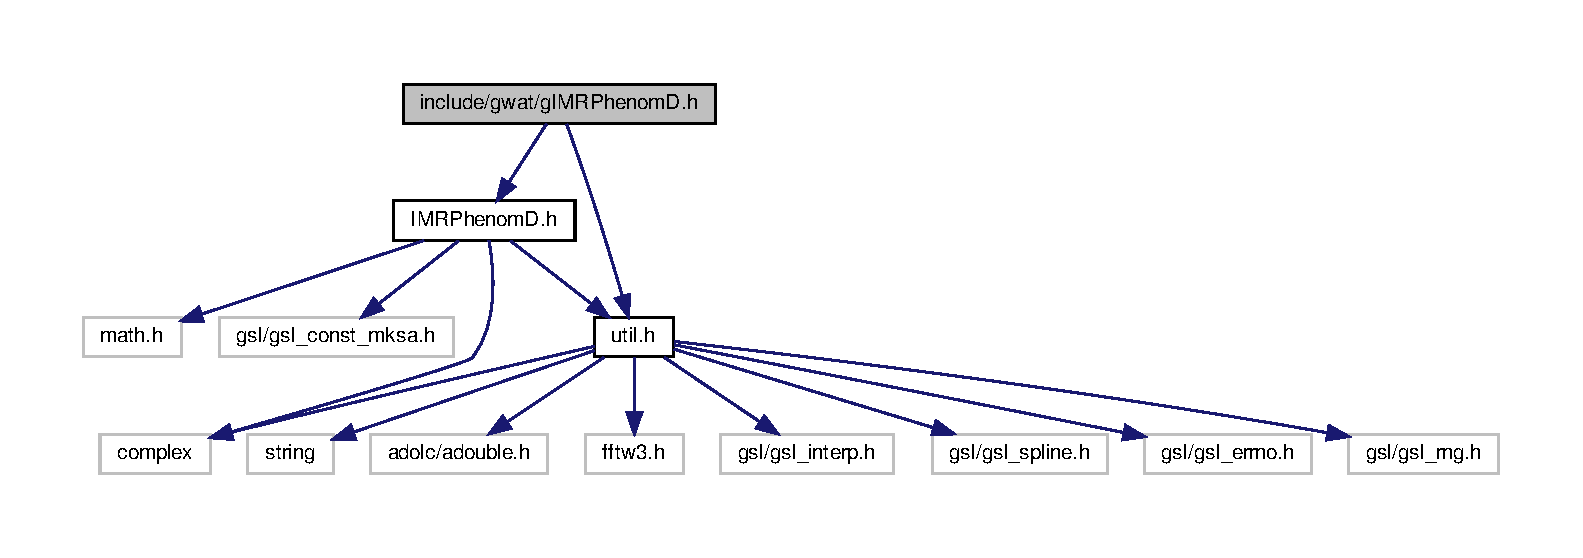
\includegraphics[width=350pt]{gIMRPhenomD_8h__incl}
\end{center}
\end{figure}
This graph shows which files directly or indirectly include this file\+:
\nopagebreak
\begin{figure}[H]
\begin{center}
\leavevmode
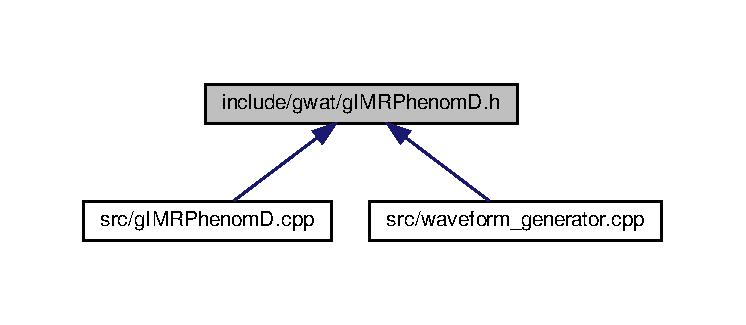
\includegraphics[width=350pt]{gIMRPhenomD_8h__dep__incl}
\end{center}
\end{figure}
\doxysubsection*{Classes}
\begin{DoxyCompactItemize}
\item 
class \mbox{\hyperlink{classgIMRPhenomD}{g\+I\+M\+R\+Phenom\+D$<$ T $>$}}
\end{DoxyCompactItemize}


\doxysubsection{Detailed Description}
Header file for \mbox{\hyperlink{classgIMRPhenomD}{g\+I\+M\+R\+PhenomD}} 
\hypertarget{GWATConfig_8h}{}\doxysection{include/gwat/\+G\+W\+A\+T\+Config.h File Reference}
\label{GWATConfig_8h}\index{include/gwat/GWATConfig.h@{include/gwat/GWATConfig.h}}
This graph shows which files directly or indirectly include this file\+:
\nopagebreak
\begin{figure}[H]
\begin{center}
\leavevmode
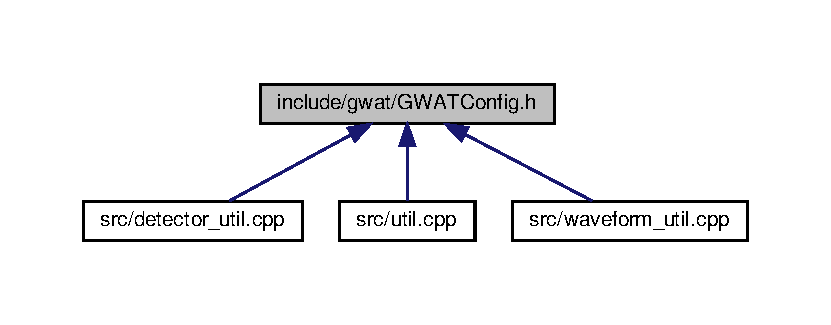
\includegraphics[width=350pt]{GWATConfig_8h__dep__incl}
\end{center}
\end{figure}
\doxysubsection*{Macros}
\begin{DoxyCompactItemize}
\item 
\mbox{\Hypertarget{GWATConfig_8h_aa470acbd74f21364919b94af9bc46d28}\label{GWATConfig_8h_aa470acbd74f21364919b94af9bc46d28}} 
\#define {\bfseries G\+W\+A\+T\+\_\+\+V\+E\+R\+S\+I\+O\+N\+\_\+\+M\+A\+J\+OR}~1
\item 
\mbox{\Hypertarget{GWATConfig_8h_abe6b70b471801de85b7ffe95caad8887}\label{GWATConfig_8h_abe6b70b471801de85b7ffe95caad8887}} 
\#define {\bfseries G\+W\+A\+T\+\_\+\+V\+E\+R\+S\+I\+O\+N\+\_\+\+M\+I\+N\+OR}~0
\item 
\mbox{\Hypertarget{GWATConfig_8h_a9f4ba46ed2bc8b78586fbd1c6a2f4b21}\label{GWATConfig_8h_a9f4ba46ed2bc8b78586fbd1c6a2f4b21}} 
\#define {\bfseries G\+W\+A\+T\+\_\+\+R\+O\+O\+T\+\_\+\+D\+I\+R\+E\+C\+T\+O\+RY}~\char`\"{}/Users/sperkins/git-\/repos/gw\+\_\+analysis\+\_\+tools/\char`\"{}
\end{DoxyCompactItemize}


\doxysubsection{Detailed Description}
Configuration file containing parameters relevant to a specific installation of G\+W\+AT

Should not have to edit -- taken care of in the makefile 
\hypertarget{IMRPhenomD_8h}{}\doxysection{include/gwat/\+I\+M\+R\+PhenomD.h File Reference}
\label{IMRPhenomD_8h}\index{include/gwat/IMRPhenomD.h@{include/gwat/IMRPhenomD.h}}
{\ttfamily \#include $<$math.\+h$>$}\newline
{\ttfamily \#include $<$gsl/gsl\+\_\+const\+\_\+mksa.\+h$>$}\newline
{\ttfamily \#include $<$complex$>$}\newline
{\ttfamily \#include \char`\"{}util.\+h\char`\"{}}\newline
Include dependency graph for I\+M\+R\+Phenom\+D.\+h\+:
\nopagebreak
\begin{figure}[H]
\begin{center}
\leavevmode
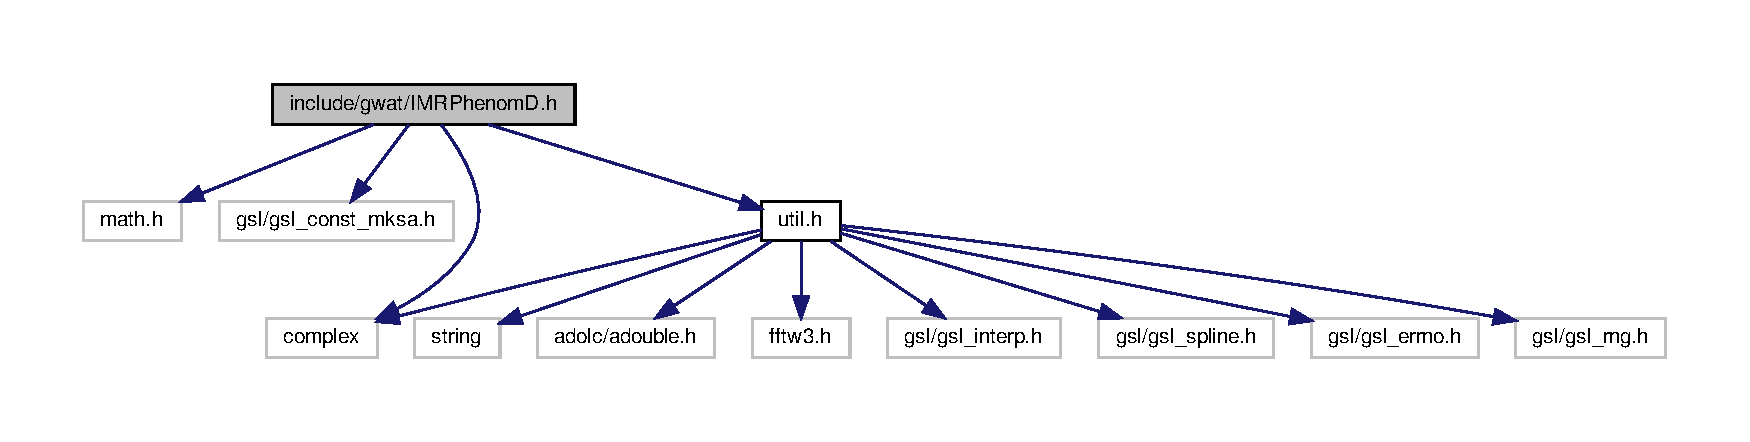
\includegraphics[width=350pt]{IMRPhenomD_8h__incl}
\end{center}
\end{figure}
This graph shows which files directly or indirectly include this file\+:
\nopagebreak
\begin{figure}[H]
\begin{center}
\leavevmode
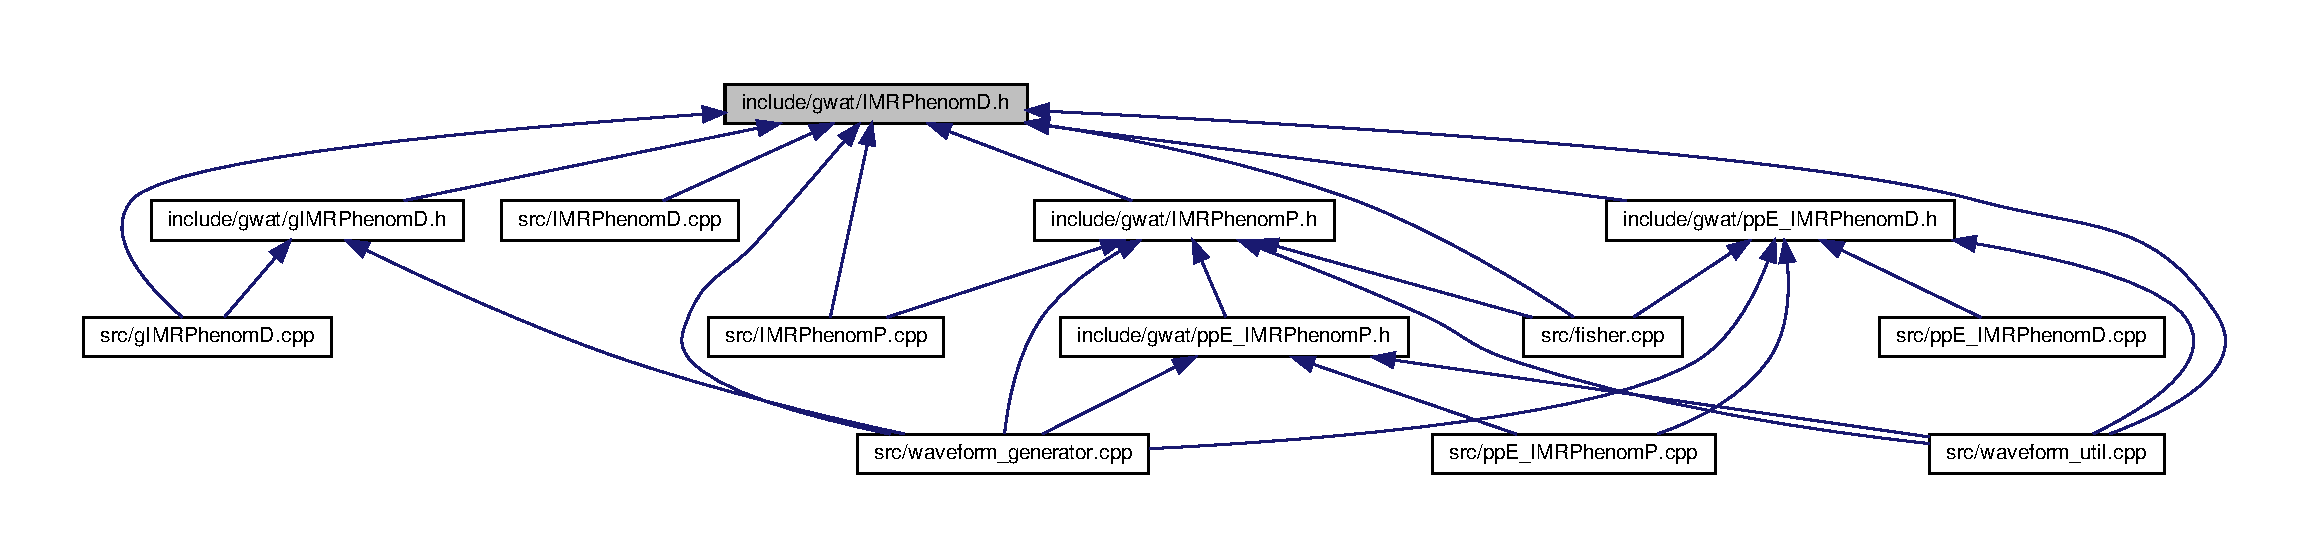
\includegraphics[width=350pt]{IMRPhenomD_8h__dep__incl}
\end{center}
\end{figure}
\doxysubsection*{Classes}
\begin{DoxyCompactItemize}
\item 
struct \mbox{\hyperlink{structlambda__parameters}{lambda\+\_\+parameters$<$ T $>$}}
\item 
class \mbox{\hyperlink{classIMRPhenomD}{I\+M\+R\+Phenom\+D$<$ T $>$}}
\end{DoxyCompactItemize}
\doxysubsection*{Variables}
\begin{DoxyCompactItemize}
\item 
const double \mbox{\hyperlink{IMRPhenomD_8h_ab4244995783dcaa1f99791db55aeb118}{lambda\+\_\+num\+\_\+params}} \mbox{[}19\mbox{]}\mbox{[}11\mbox{]}
\end{DoxyCompactItemize}


\doxysubsection{Detailed Description}
Header file for utilities 

\doxysubsection{Variable Documentation}
\mbox{\Hypertarget{IMRPhenomD_8h_ab4244995783dcaa1f99791db55aeb118}\label{IMRPhenomD_8h_ab4244995783dcaa1f99791db55aeb118}} 
\index{IMRPhenomD.h@{IMRPhenomD.h}!lambda\_num\_params@{lambda\_num\_params}}
\index{lambda\_num\_params@{lambda\_num\_params}!IMRPhenomD.h@{IMRPhenomD.h}}
\doxysubsubsection{\texorpdfstring{lambda\_num\_params}{lambda\_num\_params}}
{\footnotesize\ttfamily const double lambda\+\_\+num\+\_\+params\mbox{[}19\mbox{]}\mbox{[}11\mbox{]}}

Numerically calibrated parameters from ar\+Xiv\+:1508.\+07253 see the table in the data directory for labeled version from lalsuite 
\hypertarget{IMRPhenomP_8h}{}\doxysection{include/gwat/\+I\+M\+R\+PhenomP.h File Reference}
\label{IMRPhenomP_8h}\index{include/gwat/IMRPhenomP.h@{include/gwat/IMRPhenomP.h}}
{\ttfamily \#include \char`\"{}I\+M\+R\+Phenom\+D.\+h\char`\"{}}\newline
{\ttfamily \#include \char`\"{}util.\+h\char`\"{}}\newline
Include dependency graph for I\+M\+R\+Phenom\+P.\+h\+:
% FIG 0
This graph shows which files directly or indirectly include this file\+:
% FIG 1
\doxysubsection*{Classes}
\begin{DoxyCompactItemize}
\item 
struct \mbox{\hyperlink{structalpha__coeffs}{alpha\+\_\+coeffs$<$ T $>$}}
\item 
struct \mbox{\hyperlink{structepsilon__coeffs}{epsilon\+\_\+coeffs$<$ T $>$}}
\item 
class \mbox{\hyperlink{classIMRPhenomPv2}{I\+M\+R\+Phenom\+Pv2$<$ T $>$}}
\end{DoxyCompactItemize}


\doxysubsection{Detailed Description}
Header file for I\+M\+R\+PhenomP functions

Currently, only Pv2 is supported.

Wrapped around \mbox{\hyperlink{classIMRPhenomD}{I\+M\+R\+PhenomD}} 
\hypertarget{io__util_8h}{}\doxysection{include/gwat/io\+\_\+util.h File Reference}
\label{io__util_8h}\index{include/gwat/io\_util.h@{include/gwat/io\_util.h}}
{\ttfamily \#include $<$string$>$}\newline
{\ttfamily \#include $<$unordered\+\_\+map$>$}\newline
{\ttfamily \#include $<$complex$>$}\newline
Include dependency graph for io\+\_\+util.\+h\+:
\nopagebreak
\begin{figure}[H]
\begin{center}
\leavevmode
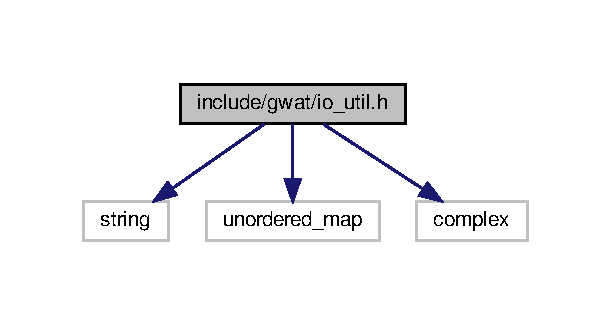
\includegraphics[width=293pt]{io__util_8h__incl}
\end{center}
\end{figure}
This graph shows which files directly or indirectly include this file\+:
\nopagebreak
\begin{figure}[H]
\begin{center}
\leavevmode
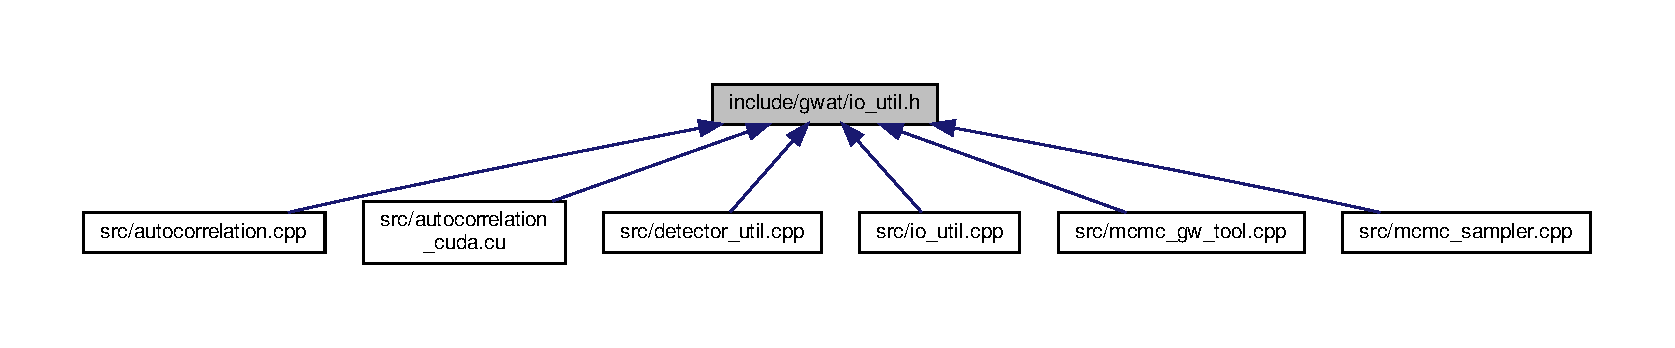
\includegraphics[width=350pt]{io__util_8h__dep__incl}
\end{center}
\end{figure}
\doxysubsection*{Functions}
\begin{DoxyCompactItemize}
\item 
\mbox{\Hypertarget{io__util_8h_ae64c41a8d5a46054427d281f7febf234}\label{io__util_8h_ae64c41a8d5a46054427d281f7febf234}} 
int {\bfseries unpack\+\_\+input\+\_\+io\+\_\+file} (std\+::string input\+\_\+param\+\_\+file, std\+::unordered\+\_\+map$<$ std\+::string, int $>$ $\ast$input\+\_\+param\+\_\+dict\+\_\+int, std\+::unordered\+\_\+map$<$ std\+::string, std\+::string $>$ $\ast$input\+\_\+param\+\_\+dict\+\_\+str, std\+::unordered\+\_\+map$<$ std\+::string, double $>$ $\ast$input\+\_\+param\+\_\+dict\+\_\+dbl, std\+::unordered\+\_\+map$<$ std\+::string, float $>$ $\ast$input\+\_\+param\+\_\+dict\+\_\+flt, std\+::unordered\+\_\+map$<$ std\+::string, bool $>$ $\ast$input\+\_\+param\+\_\+dict\+\_\+bool)
\item 
int \mbox{\hyperlink{io__util_8h_a627ac895351aa8f4c26a2565cf1769d0}{find\+\_\+datatype}} (std\+::string type)
\begin{DoxyCompactList}\small\item\em Takes in the shorthand for primitive datatypes in c++ and returns code based on type. \end{DoxyCompactList}\item 
\mbox{\Hypertarget{io__util_8h_a9b855aac79a01bc69b093a4ee12bb688}\label{io__util_8h_a9b855aac79a01bc69b093a4ee12bb688}} 
std\+::string {\bfseries trim} (std\+::string str)
\item 
void \mbox{\hyperlink{io__util_8h_aad742282a09bb261d21080e8874578ba}{read\+\_\+file}} (std\+::string filename, double $\ast$$\ast$output, int rows, int cols)
\begin{DoxyCompactList}\small\item\em Utility to read in data. \end{DoxyCompactList}\item 
void \mbox{\hyperlink{io__util_8h_abed5d6708a7adc8cd37ca0d578730b17}{read\+\_\+file}} (std\+::string filename, int $\ast$$\ast$output, int rows, int cols)
\begin{DoxyCompactList}\small\item\em Utility to read in data. \end{DoxyCompactList}\item 
void \mbox{\hyperlink{io__util_8h_a788a44b839a09910024159d9d10764d0}{read\+\_\+file}} (std\+::string filename, double $\ast$output)
\begin{DoxyCompactList}\small\item\em Utility to read in data (single dimension vector) \end{DoxyCompactList}\item 
void \mbox{\hyperlink{io__util_8h_a6add7454e404e8305cd6695b0cff428e}{read\+\_\+file}} (std\+::string filename, int $\ast$output)
\begin{DoxyCompactList}\small\item\em Utility to read in data (single dimension vector) \end{DoxyCompactList}\item 
void \mbox{\hyperlink{io__util_8h_a8cb10f1eb5598be2a3aa53dcc2ebe844}{write\+\_\+file}} (std\+::string filename, double $\ast$$\ast$input, int rows, int cols)
\begin{DoxyCompactList}\small\item\em Utility to write 2D array to file. \end{DoxyCompactList}\item 
void \mbox{\hyperlink{io__util_8h_a4b7b68907ec287799769dd0a1ff0b427}{write\+\_\+file}} (std\+::string filename, int $\ast$$\ast$input, int rows, int cols)
\begin{DoxyCompactList}\small\item\em Utility to write 2D array to file. \end{DoxyCompactList}\item 
void \mbox{\hyperlink{io__util_8h_a2364e735eddfa67c1317f6ebc64565f3}{write\+\_\+file}} (std\+::string filename, double $\ast$input, int length)
\begin{DoxyCompactList}\small\item\em Utility to write 1D array to file. \end{DoxyCompactList}\item 
void \mbox{\hyperlink{io__util_8h_ab6683e37f11111fe729fe0fd304c5651}{write\+\_\+file}} (std\+::string filename, int $\ast$input, int length)
\begin{DoxyCompactList}\small\item\em Utility to write 1D array to file. \end{DoxyCompactList}\item 
void \mbox{\hyperlink{io__util_8h_abbb4e70ddc93c8995739b3a481bbf3a6}{read\+\_\+\+L\+O\+S\+C\+\_\+data\+\_\+file}} (std\+::string filename, double $\ast$output, double $\ast$data\+\_\+start\+\_\+time, double $\ast$duration, double $\ast$fs)
\begin{DoxyCompactList}\small\item\em Read data file from L\+I\+GO Open Science Center. \end{DoxyCompactList}\item 
void \mbox{\hyperlink{io__util_8h_a089aa96b136d368b0c740c416811c39d}{read\+\_\+\+L\+O\+S\+C\+\_\+\+P\+S\+D\+\_\+file}} (std\+::string filename, double $\ast$$\ast$output, int rows, int cols)
\begin{DoxyCompactList}\small\item\em Read P\+SD file from L\+I\+GO Open Science Center. \end{DoxyCompactList}\item 
void \mbox{\hyperlink{io__util_8h_aa73bbfc171abf859eff4c14e07ed1e0a}{allocate\+\_\+\+L\+O\+S\+C\+\_\+data}} (std\+::string $\ast$data\+\_\+files, std\+::string psd\+\_\+file, int num\+\_\+detectors, int psd\+\_\+length, int data\+\_\+file\+\_\+length, double trigger\+\_\+time, std\+::complex$<$ double $>$ $\ast$$\ast$data, double $\ast$$\ast$psds, double $\ast$$\ast$freqs)
\begin{DoxyCompactList}\small\item\em Prepare data for M\+C\+MC directly from L\+I\+GO Open Science Center. \end{DoxyCompactList}\item 
void \mbox{\hyperlink{io__util_8h_a3196bd767443186731edcfc84e43ac93}{free\+\_\+\+L\+O\+S\+C\+\_\+data}} (std\+::complex$<$ double $>$ $\ast$$\ast$data, double $\ast$$\ast$psds, double $\ast$$\ast$freqs, int num\+\_\+detectors, int length)
\item 
\mbox{\Hypertarget{io__util_8h_aabb38ec649dc87bca9ddd9ddd1baea78}\label{io__util_8h_aabb38ec649dc87bca9ddd9ddd1baea78}} 
int \mbox{\hyperlink{io__util_8h_aabb38ec649dc87bca9ddd9ddd1baea78}{count\+\_\+lines\+\_\+data\+\_\+file}} (std\+::string file, int $\ast$count)
\begin{DoxyCompactList}\small\item\em Takes in data file and returns the number of data elements in file. \end{DoxyCompactList}\item 
\mbox{\Hypertarget{io__util_8h_aaf15f8db5f36caf636d88f41e29b17be}\label{io__util_8h_aaf15f8db5f36caf636d88f41e29b17be}} 
int \mbox{\hyperlink{io__util_8h_aaf15f8db5f36caf636d88f41e29b17be}{count\+\_\+lines\+\_\+\+L\+O\+S\+C\+\_\+\+P\+S\+D\+\_\+file}} (std\+::string file, int $\ast$count)
\begin{DoxyCompactList}\small\item\em Takes in L\+O\+SC P\+SD file and returns the number of data elements in file. \end{DoxyCompactList}\item 
\mbox{\Hypertarget{io__util_8h_a2d2ec12ff7cb75ea68ec4139513bab4c}\label{io__util_8h_a2d2ec12ff7cb75ea68ec4139513bab4c}} 
int \mbox{\hyperlink{io__util_8h_a2d2ec12ff7cb75ea68ec4139513bab4c}{count\+\_\+lines\+\_\+\+L\+O\+S\+C\+\_\+data\+\_\+file}} (std\+::string file, int $\ast$count)
\begin{DoxyCompactList}\small\item\em Takes in L\+O\+SC data file and returns the number of data elements in file. \end{DoxyCompactList}\end{DoxyCompactItemize}


\doxysubsection{Function Documentation}
\mbox{\Hypertarget{io__util_8h_aa73bbfc171abf859eff4c14e07ed1e0a}\label{io__util_8h_aa73bbfc171abf859eff4c14e07ed1e0a}} 
\index{io\_util.h@{io\_util.h}!allocate\_LOSC\_data@{allocate\_LOSC\_data}}
\index{allocate\_LOSC\_data@{allocate\_LOSC\_data}!io\_util.h@{io\_util.h}}
\doxysubsubsection{\texorpdfstring{allocate\_LOSC\_data()}{allocate\_LOSC\_data()}}
{\footnotesize\ttfamily void allocate\+\_\+\+L\+O\+S\+C\+\_\+data (\begin{DoxyParamCaption}\item[{std\+::string $\ast$}]{data\+\_\+files,  }\item[{std\+::string}]{psd\+\_\+file,  }\item[{int}]{num\+\_\+detectors,  }\item[{int}]{psd\+\_\+length,  }\item[{int}]{data\+\_\+file\+\_\+length,  }\item[{double}]{trigger\+\_\+time,  }\item[{std\+::complex$<$ double $>$ $\ast$$\ast$}]{data,  }\item[{double $\ast$$\ast$}]{psds,  }\item[{double $\ast$$\ast$}]{freqs }\end{DoxyParamCaption})}



Prepare data for M\+C\+MC directly from L\+I\+GO Open Science Center. 

Trims data for Tobs (determined by P\+SD file) 3/4$\ast$\+Tobs in front of trigger, and 1/4$\ast$\+Tobs behind

Currently, default to sampling frequency and observation time set by P\+SD -- cannot be customized

Output is in order of P\+SD columns -- string vector of detectos M\+U\+ST match order of P\+SD cols

Output shapes-- \begin{DoxyVerb}    psds = [num_detectors][psd_length]

    data = [num_detectors][psd_length]  

    freqs = [num_detectors][psd_length] 
\end{DoxyVerb}


Total observation time = 1/( freq\mbox{[}i\mbox{]} -\/ freq\mbox{[}i-\/1\mbox{]}) (from P\+SD file)

Sampling frequency fs = max frequency from P\+SD file

A\+L\+L\+O\+C\+A\+T\+ES M\+E\+M\+O\+RY -- must be freed to prevent memory leak 
\begin{DoxyParams}[1]{Parameters}
 & {\em data\+\_\+files} & Vector of strings for each detector file from L\+O\+SC \\
\hline
 & {\em psd\+\_\+file} & String of psd file from L\+O\+SC \\
\hline
 & {\em num\+\_\+detectors} & Number of detectors to use \\
\hline
 & {\em psd\+\_\+length} & Length of the P\+SD file (number of rows of D\+A\+TA) \\
\hline
 & {\em data\+\_\+file\+\_\+length} & Length of the data file (number of rows of D\+A\+TA) \\
\hline
 & {\em trigger\+\_\+time} & Time for the signal trigger (G\+PS) \\
\hline
\mbox{\texttt{ out}}  & {\em data} & Output array of data for each detector \\
\hline
\mbox{\texttt{ out}}  & {\em psds} & Output array of psds for each detector \\
\hline
\mbox{\texttt{ out}}  & {\em freqs} & Output array of freqs for each detector \\
\hline
\end{DoxyParams}
\mbox{\Hypertarget{io__util_8h_a627ac895351aa8f4c26a2565cf1769d0}\label{io__util_8h_a627ac895351aa8f4c26a2565cf1769d0}} 
\index{io\_util.h@{io\_util.h}!find\_datatype@{find\_datatype}}
\index{find\_datatype@{find\_datatype}!io\_util.h@{io\_util.h}}
\doxysubsubsection{\texorpdfstring{find\_datatype()}{find\_datatype()}}
{\footnotesize\ttfamily int find\+\_\+datatype (\begin{DoxyParamCaption}\item[{std\+::string}]{type }\end{DoxyParamCaption})}



Takes in the shorthand for primitive datatypes in c++ and returns code based on type. 

Returns\+: \begin{DoxyVerb}0 -- Not found

1 -- int

2 -- string

3 -- double

4 -- float

5 -- bool
\end{DoxyVerb}
 \mbox{\Hypertarget{io__util_8h_a3196bd767443186731edcfc84e43ac93}\label{io__util_8h_a3196bd767443186731edcfc84e43ac93}} 
\index{io\_util.h@{io\_util.h}!free\_LOSC\_data@{free\_LOSC\_data}}
\index{free\_LOSC\_data@{free\_LOSC\_data}!io\_util.h@{io\_util.h}}
\doxysubsubsection{\texorpdfstring{free\_LOSC\_data()}{free\_LOSC\_data()}}
{\footnotesize\ttfamily void free\+\_\+\+L\+O\+S\+C\+\_\+data (\begin{DoxyParamCaption}\item[{std\+::complex$<$ double $>$ $\ast$$\ast$}]{data,  }\item[{double $\ast$$\ast$}]{psds,  }\item[{double $\ast$$\ast$}]{freqs,  }\item[{int}]{num\+\_\+detectors,  }\item[{int}]{length }\end{DoxyParamCaption})}

/brief Free data allocated by prep\+\_\+\+L\+O\+S\+C\+\_\+data function \mbox{\Hypertarget{io__util_8h_aad742282a09bb261d21080e8874578ba}\label{io__util_8h_aad742282a09bb261d21080e8874578ba}} 
\index{io\_util.h@{io\_util.h}!read\_file@{read\_file}}
\index{read\_file@{read\_file}!io\_util.h@{io\_util.h}}
\doxysubsubsection{\texorpdfstring{read\_file()}{read\_file()}\hspace{0.1cm}{\footnotesize\ttfamily [1/4]}}
{\footnotesize\ttfamily void read\+\_\+file (\begin{DoxyParamCaption}\item[{std\+::string}]{filename,  }\item[{double $\ast$$\ast$}]{output,  }\item[{int}]{rows,  }\item[{int}]{cols }\end{DoxyParamCaption})}



Utility to read in data. 

Takes filename, and assigns to output\mbox{[}rows\mbox{]}\mbox{[}cols\mbox{]}

File must be comma separated doubles 
\begin{DoxyParams}[1]{Parameters}
 & {\em filename} & input filename, relative to execution directory \\
\hline
\mbox{\texttt{ out}}  & {\em output} & array to store output, dimensions rows\+Xcols \\
\hline
 & {\em rows} & first dimension \\
\hline
 & {\em cols} & second dimension \\
\hline
\end{DoxyParams}
\mbox{\Hypertarget{io__util_8h_a788a44b839a09910024159d9d10764d0}\label{io__util_8h_a788a44b839a09910024159d9d10764d0}} 
\index{io\_util.h@{io\_util.h}!read\_file@{read\_file}}
\index{read\_file@{read\_file}!io\_util.h@{io\_util.h}}
\doxysubsubsection{\texorpdfstring{read\_file()}{read\_file()}\hspace{0.1cm}{\footnotesize\ttfamily [2/4]}}
{\footnotesize\ttfamily void read\+\_\+file (\begin{DoxyParamCaption}\item[{std\+::string}]{filename,  }\item[{double $\ast$}]{output }\end{DoxyParamCaption})}



Utility to read in data (single dimension vector) 

Takes filename, and assigns to output\mbox{[}i$\ast$rows + cols\mbox{]}

Output vector must be long enough, no check is done for the length

File must be comma separated doubles 
\begin{DoxyParams}[1]{Parameters}
 & {\em filename} & input filename, relative to execution directory \\
\hline
\mbox{\texttt{ out}}  & {\em output} & output array, assumed to have the proper length of total items \\
\hline
\end{DoxyParams}
\mbox{\Hypertarget{io__util_8h_abed5d6708a7adc8cd37ca0d578730b17}\label{io__util_8h_abed5d6708a7adc8cd37ca0d578730b17}} 
\index{io\_util.h@{io\_util.h}!read\_file@{read\_file}}
\index{read\_file@{read\_file}!io\_util.h@{io\_util.h}}
\doxysubsubsection{\texorpdfstring{read\_file()}{read\_file()}\hspace{0.1cm}{\footnotesize\ttfamily [3/4]}}
{\footnotesize\ttfamily void read\+\_\+file (\begin{DoxyParamCaption}\item[{std\+::string}]{filename,  }\item[{int $\ast$$\ast$}]{output,  }\item[{int}]{rows,  }\item[{int}]{cols }\end{DoxyParamCaption})}



Utility to read in data. 

Takes filename, and assigns to output\mbox{[}rows\mbox{]}\mbox{[}cols\mbox{]}

File must be comma separated doubles

integer version 
\begin{DoxyParams}[1]{Parameters}
 & {\em filename} & input filename, relative to execution directory \\
\hline
\mbox{\texttt{ out}}  & {\em output} & array to store output, dimensions rows\+Xcols \\
\hline
 & {\em rows} & first dimension \\
\hline
 & {\em cols} & second dimension \\
\hline
\end{DoxyParams}
\mbox{\Hypertarget{io__util_8h_a6add7454e404e8305cd6695b0cff428e}\label{io__util_8h_a6add7454e404e8305cd6695b0cff428e}} 
\index{io\_util.h@{io\_util.h}!read\_file@{read\_file}}
\index{read\_file@{read\_file}!io\_util.h@{io\_util.h}}
\doxysubsubsection{\texorpdfstring{read\_file()}{read\_file()}\hspace{0.1cm}{\footnotesize\ttfamily [4/4]}}
{\footnotesize\ttfamily void read\+\_\+file (\begin{DoxyParamCaption}\item[{std\+::string}]{filename,  }\item[{int $\ast$}]{output }\end{DoxyParamCaption})}



Utility to read in data (single dimension vector) 

Takes filename, and assigns to output\mbox{[}i$\ast$rows + cols\mbox{]}

Output vector must be long enough, no check is done for the length

File must be comma separated doubles

Int version 
\begin{DoxyParams}[1]{Parameters}
 & {\em filename} & input filename, relative to execution directory \\
\hline
\mbox{\texttt{ out}}  & {\em output} & output array, assumed to have the proper length of total items \\
\hline
\end{DoxyParams}
\mbox{\Hypertarget{io__util_8h_abbb4e70ddc93c8995739b3a481bbf3a6}\label{io__util_8h_abbb4e70ddc93c8995739b3a481bbf3a6}} 
\index{io\_util.h@{io\_util.h}!read\_LOSC\_data\_file@{read\_LOSC\_data\_file}}
\index{read\_LOSC\_data\_file@{read\_LOSC\_data\_file}!io\_util.h@{io\_util.h}}
\doxysubsubsection{\texorpdfstring{read\_LOSC\_data\_file()}{read\_LOSC\_data\_file()}}
{\footnotesize\ttfamily void read\+\_\+\+L\+O\+S\+C\+\_\+data\+\_\+file (\begin{DoxyParamCaption}\item[{std\+::string}]{filename,  }\item[{double $\ast$}]{output,  }\item[{double $\ast$}]{data\+\_\+start\+\_\+time,  }\item[{double $\ast$}]{duration,  }\item[{double $\ast$}]{fs }\end{DoxyParamCaption})}



Read data file from L\+I\+GO Open Science Center. 

Convenience function for cutting off the first few lines of text 
\begin{DoxyParams}[1]{Parameters}
 & {\em filename} & input filename \\
\hline
\mbox{\texttt{ out}}  & {\em output} & Output data \\
\hline
\mbox{\texttt{ out}}  & {\em data\+\_\+start\+\_\+time} & G\+PS start time of the data in file \\
\hline
\mbox{\texttt{ out}}  & {\em duration} & Duration of the signal \\
\hline
\mbox{\texttt{ out}}  & {\em fs} & Sampling frequency of the data \\
\hline
\end{DoxyParams}
\mbox{\Hypertarget{io__util_8h_a089aa96b136d368b0c740c416811c39d}\label{io__util_8h_a089aa96b136d368b0c740c416811c39d}} 
\index{io\_util.h@{io\_util.h}!read\_LOSC\_PSD\_file@{read\_LOSC\_PSD\_file}}
\index{read\_LOSC\_PSD\_file@{read\_LOSC\_PSD\_file}!io\_util.h@{io\_util.h}}
\doxysubsubsection{\texorpdfstring{read\_LOSC\_PSD\_file()}{read\_LOSC\_PSD\_file()}}
{\footnotesize\ttfamily void read\+\_\+\+L\+O\+S\+C\+\_\+\+P\+S\+D\+\_\+file (\begin{DoxyParamCaption}\item[{std\+::string}]{filename,  }\item[{double $\ast$$\ast$}]{output,  }\item[{int}]{rows,  }\item[{int}]{cols }\end{DoxyParamCaption})}



Read P\+SD file from L\+I\+GO Open Science Center. 

Convenience function for cutting off the first few lines of text \mbox{\Hypertarget{io__util_8h_a8cb10f1eb5598be2a3aa53dcc2ebe844}\label{io__util_8h_a8cb10f1eb5598be2a3aa53dcc2ebe844}} 
\index{io\_util.h@{io\_util.h}!write\_file@{write\_file}}
\index{write\_file@{write\_file}!io\_util.h@{io\_util.h}}
\doxysubsubsection{\texorpdfstring{write\_file()}{write\_file()}\hspace{0.1cm}{\footnotesize\ttfamily [1/4]}}
{\footnotesize\ttfamily void write\+\_\+file (\begin{DoxyParamCaption}\item[{std\+::string}]{filename,  }\item[{double $\ast$$\ast$}]{input,  }\item[{int}]{rows,  }\item[{int}]{cols }\end{DoxyParamCaption})}



Utility to write 2D array to file. 

Grid of data, comma separated

Grid has rows rows and cols columns 
\begin{DoxyParams}{Parameters}
{\em filename} & Filename of output file, relative to execution directory \\
\hline
{\em input} & Input 2D array pointer array\mbox{[}rows\mbox{]}\mbox{[}cols\mbox{]} \\
\hline
{\em rows} & First dimension of array \\
\hline
{\em cols} & second dimension of array \\
\hline
\end{DoxyParams}
\mbox{\Hypertarget{io__util_8h_a2364e735eddfa67c1317f6ebc64565f3}\label{io__util_8h_a2364e735eddfa67c1317f6ebc64565f3}} 
\index{io\_util.h@{io\_util.h}!write\_file@{write\_file}}
\index{write\_file@{write\_file}!io\_util.h@{io\_util.h}}
\doxysubsubsection{\texorpdfstring{write\_file()}{write\_file()}\hspace{0.1cm}{\footnotesize\ttfamily [2/4]}}
{\footnotesize\ttfamily void write\+\_\+file (\begin{DoxyParamCaption}\item[{std\+::string}]{filename,  }\item[{double $\ast$}]{input,  }\item[{int}]{length }\end{DoxyParamCaption})}



Utility to write 1D array to file. 

Single column of data 
\begin{DoxyParams}{Parameters}
{\em filename} & Filename of output file, relative to execution directory \\
\hline
{\em input} & input 1D array pointer array\mbox{[}length\mbox{]} \\
\hline
{\em length} & length of array \\
\hline
\end{DoxyParams}
\mbox{\Hypertarget{io__util_8h_a4b7b68907ec287799769dd0a1ff0b427}\label{io__util_8h_a4b7b68907ec287799769dd0a1ff0b427}} 
\index{io\_util.h@{io\_util.h}!write\_file@{write\_file}}
\index{write\_file@{write\_file}!io\_util.h@{io\_util.h}}
\doxysubsubsection{\texorpdfstring{write\_file()}{write\_file()}\hspace{0.1cm}{\footnotesize\ttfamily [3/4]}}
{\footnotesize\ttfamily void write\+\_\+file (\begin{DoxyParamCaption}\item[{std\+::string}]{filename,  }\item[{int $\ast$$\ast$}]{input,  }\item[{int}]{rows,  }\item[{int}]{cols }\end{DoxyParamCaption})}



Utility to write 2D array to file. 

Grid of data, comma separated

Grid has rows rows and cols columns

integer version 
\begin{DoxyParams}{Parameters}
{\em filename} & Filename of output file, relative to execution directory \\
\hline
{\em input} & Input 2D array pointer array\mbox{[}rows\mbox{]}\mbox{[}cols\mbox{]} \\
\hline
{\em rows} & First dimension of array \\
\hline
{\em cols} & second dimension of array \\
\hline
\end{DoxyParams}
\mbox{\Hypertarget{io__util_8h_ab6683e37f11111fe729fe0fd304c5651}\label{io__util_8h_ab6683e37f11111fe729fe0fd304c5651}} 
\index{io\_util.h@{io\_util.h}!write\_file@{write\_file}}
\index{write\_file@{write\_file}!io\_util.h@{io\_util.h}}
\doxysubsubsection{\texorpdfstring{write\_file()}{write\_file()}\hspace{0.1cm}{\footnotesize\ttfamily [4/4]}}
{\footnotesize\ttfamily void write\+\_\+file (\begin{DoxyParamCaption}\item[{std\+::string}]{filename,  }\item[{int $\ast$}]{input,  }\item[{int}]{length }\end{DoxyParamCaption})}



Utility to write 1D array to file. 

Single column of data

integer version 
\begin{DoxyParams}{Parameters}
{\em filename} & Filename of output file, relative to execution directory \\
\hline
{\em input} & input 1D array pointer array\mbox{[}length\mbox{]} \\
\hline
{\em length} & length of array \\
\hline
\end{DoxyParams}

\hypertarget{mc__reject_8h}{}\doxysection{include/gwat/mc\+\_\+reject.h File Reference}
\label{mc__reject_8h}\index{include/gwat/mc\_reject.h@{include/gwat/mc\_reject.h}}
{\ttfamily \#include $<$functional$>$}\newline
{\ttfamily \#include $<$gsl/gsl\+\_\+rng.\+h$>$}\newline
Include dependency graph for mc\+\_\+reject.\+h\+:
\nopagebreak
\begin{figure}[H]
\begin{center}
\leavevmode
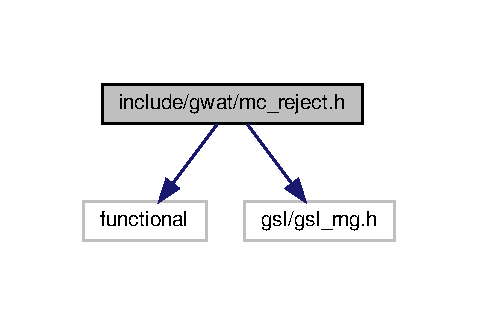
\includegraphics[width=230pt]{mc__reject_8h__incl}
\end{center}
\end{figure}
This graph shows which files directly or indirectly include this file\+:
\nopagebreak
\begin{figure}[H]
\begin{center}
\leavevmode
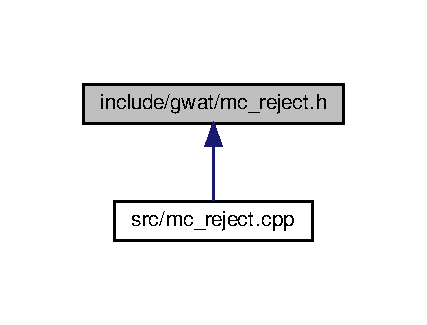
\includegraphics[width=205pt]{mc__reject_8h__dep__incl}
\end{center}
\end{figure}
\doxysubsection*{Classes}
\begin{DoxyCompactItemize}
\item 
class \mbox{\hyperlink{classmcr__sampler}{mcr\+\_\+sampler}}
\item 
struct \mbox{\hyperlink{structmcr__job}{mcr\+\_\+job}}
\end{DoxyCompactItemize}
\doxysubsection*{Functions}
\begin{DoxyCompactItemize}
\item 
void \mbox{\hyperlink{mc__reject_8h_a8e7fcdc575532164d9f76f27102b4c9a}{parallel\+\_\+sample}} (int threadid, \mbox{\hyperlink{structmcr__job}{mcr\+\_\+job}} job)
\begin{DoxyCompactList}\small\item\em internal routine to draw N samples \end{DoxyCompactList}\end{DoxyCompactItemize}


\doxysubsection{Detailed Description}
Header file for the Monte Carlo Rejection Sampler 

\doxysubsection{Function Documentation}
\mbox{\Hypertarget{mc__reject_8h_a8e7fcdc575532164d9f76f27102b4c9a}\label{mc__reject_8h_a8e7fcdc575532164d9f76f27102b4c9a}} 
\index{mc\_reject.h@{mc\_reject.h}!parallel\_sample@{parallel\_sample}}
\index{parallel\_sample@{parallel\_sample}!mc\_reject.h@{mc\_reject.h}}
\doxysubsubsection{\texorpdfstring{parallel\_sample()}{parallel\_sample()}}
{\footnotesize\ttfamily void parallel\+\_\+sample (\begin{DoxyParamCaption}\item[{int}]{threadid,  }\item[{\mbox{\hyperlink{structmcr__job}{mcr\+\_\+job}}}]{job }\end{DoxyParamCaption})}



internal routine to draw N samples 

Should not be called by the user

Just made this separate from the class for now for convenience 
\begin{DoxyParams}{Parameters}
{\em job} & mcr job -\/-\/ see \mbox{\hyperlink{mc__reject_8h}{mc\+\_\+reject.\+h}} \\
\hline
\end{DoxyParams}

\hypertarget{mcmc__gw_8h}{}\doxysection{include/gwat/mcmc\+\_\+gw.h File Reference}
\label{mcmc__gw_8h}\index{include/gwat/mcmc\_gw.h@{include/gwat/mcmc\_gw.h}}
{\ttfamily \#include $<$complex$>$}\newline
{\ttfamily \#include $<$fftw3.\+h$>$}\newline
{\ttfamily \#include \char`\"{}util.\+h\char`\"{}}\newline
{\ttfamily \#include $<$iostream$>$}\newline
{\ttfamily \#include $<$gsl/gsl\+\_\+interp.\+h$>$}\newline
{\ttfamily \#include $<$gsl/gsl\+\_\+randist.\+h$>$}\newline
{\ttfamily \#include $<$gsl/gsl\+\_\+rng.\+h$>$}\newline
{\ttfamily \#include $<$gsl/gsl\+\_\+spline.\+h$>$}\newline
{\ttfamily \#include $<$gsl/gsl\+\_\+errno.\+h$>$}\newline
Include dependency graph for mcmc\+\_\+gw.\+h\+:
% FIG 0
This graph shows which files directly or indirectly include this file\+:
% FIG 1
\doxysubsection*{Functions}
\begin{DoxyCompactItemize}
\item 
double \mbox{\hyperlink{mcmc__gw_8h_abd627450e43bf7ef683d875d804b7503}{maximized\+\_\+coal\+\_\+log\+\_\+likelihood\+\_\+\+I\+M\+R\+PhenomD}} (double $\ast$frequencies, int length, std\+::complex$<$ double $>$ $\ast$data, double $\ast$noise, double S\+NR, double chirpmass, double symmetric\+\_\+mass\+\_\+ratio, double spin1, double spin2, bool N\+Sflag, \mbox{\hyperlink{structfftw__outline}{fftw\+\_\+outline}} $\ast$plan)
\begin{DoxyCompactList}\small\item\em Function to calculate the log Likelihood as defined by -\/1/2 (d-\/h$\vert$d-\/h) maximized over the extrinsic parameters phic and tc. \end{DoxyCompactList}\item 
double \mbox{\hyperlink{mcmc__gw_8h_ae78896f8e8acd8dfaff6ff33a732284a}{maximized\+\_\+coal\+\_\+log\+\_\+likelihood\+\_\+\+I\+M\+R\+PhenomD}} (double $\ast$frequencies, size\+\_\+t length, double $\ast$real\+\_\+data, double $\ast$imag\+\_\+data, double $\ast$noise, double S\+NR, double chirpmass, double symmetric\+\_\+mass\+\_\+ratio, double spin1, double spin2, bool N\+Sflag)
\item 
double \mbox{\hyperlink{mcmc__gw_8h_a2635acb06ca0e448854aaab3fd7037c3}{maximized\+\_\+coal\+\_\+log\+\_\+likelihood\+\_\+\+I\+M\+R\+PhenomD}} (double $\ast$frequencies, size\+\_\+t length, double $\ast$real\+\_\+data, double $\ast$imag\+\_\+data, double $\ast$noise, double S\+NR, double chirpmass, double symmetric\+\_\+mass\+\_\+ratio, double spin1, double spin2, bool N\+Sflag, \mbox{\hyperlink{structfftw__outline}{fftw\+\_\+outline}} $\ast$plan)
\item 
double \mbox{\hyperlink{mcmc__gw_8h_ac66db6fc5c75ee33b84a48724b4738ef}{maximized\+\_\+coal\+\_\+log\+\_\+likelihood\+\_\+\+I\+M\+R\+Phenom\+D\+\_\+\+Full\+\_\+\+Param}} (double $\ast$frequencies, int length, std\+::complex$<$ double $>$ $\ast$data, double $\ast$noise, double chirpmass, double symmetric\+\_\+mass\+\_\+ratio, double spin1, double spin2, double Luminosity\+\_\+\+Distance, double theta, double phi, double iota, bool N\+Sflag, \mbox{\hyperlink{structfftw__outline}{fftw\+\_\+outline}} $\ast$plan)
\item 
double \mbox{\hyperlink{mcmc__gw_8h_a2322ab4b42380145e742ad564c643874}{maximized\+\_\+coal\+\_\+log\+\_\+likelihood\+\_\+\+I\+M\+R\+Phenom\+D\+\_\+\+Full\+\_\+\+Param}} (double $\ast$frequencies, size\+\_\+t length, double $\ast$real\+\_\+data, double $\ast$imag\+\_\+data, double $\ast$noise, double chirpmass, double symmetric\+\_\+mass\+\_\+ratio, double spin1, double spin2, double Luminosity\+\_\+\+Distance, double theta, double phi, double iota, bool N\+Sflag)
\item 
double \mbox{\hyperlink{mcmc__gw_8h_a3fbdbcf0651bad5541eb6e366c62de23}{maximized\+\_\+coal\+\_\+log\+\_\+likelihood\+\_\+\+I\+M\+R\+Phenom\+D\+\_\+\+Full\+\_\+\+Param}} (double $\ast$frequencies, size\+\_\+t length, double $\ast$real\+\_\+data, double $\ast$imag\+\_\+data, double $\ast$noise, double chirpmass, double symmetric\+\_\+mass\+\_\+ratio, double spin1, double spin2, double Luminosity\+\_\+\+Distance, double theta, double phi, double iota, bool N\+Sflag, \mbox{\hyperlink{structfftw__outline}{fftw\+\_\+outline}} $\ast$plan)
\item 
double \mbox{\hyperlink{mcmc__gw_8h_aecba6e7ba4f5a7463c95e0d65cfb3145}{maximized\+\_\+\+Log\+\_\+\+Likelihood\+\_\+aligned\+\_\+spin\+\_\+internal}} (std\+::complex$<$ double $>$ $\ast$data, double $\ast$psd, double $\ast$frequencies, std\+::complex$<$ double $>$ $\ast$detector\+\_\+response, size\+\_\+t length, \mbox{\hyperlink{structfftw__outline}{fftw\+\_\+outline}} $\ast$plan)
\begin{DoxyCompactList}\small\item\em Maximized match over coalescence variables -\/ returns log likelihood N\+OT N\+O\+R\+M\+A\+L\+I\+Z\+ED for aligned spins. \end{DoxyCompactList}\item 
double \mbox{\hyperlink{mcmc__gw_8h_ac631d3718500bb00b10e14e4d5e62adf}{Log\+\_\+\+Likelihood}} (std\+::complex$<$ double $>$ $\ast$data, double $\ast$psd, double $\ast$frequencies, size\+\_\+t length, \mbox{\hyperlink{classgen__params__base}{gen\+\_\+params\+\_\+base}}$<$ double $>$ $\ast$params, std\+::string detector, std\+::string generation\+\_\+method, \mbox{\hyperlink{structfftw__outline}{fftw\+\_\+outline}} $\ast$plan)
\begin{DoxyCompactList}\small\item\em Unmarginalized log of the likelihood. \end{DoxyCompactList}\item 
double \mbox{\hyperlink{mcmc__gw_8h_a2c44e4b3acd713ae4ad07b92b96ac017}{maximized\+\_\+\+Log\+\_\+\+Likelihood\+\_\+unaligned\+\_\+spin\+\_\+internal}} (std\+::complex$<$ double $>$ $\ast$data, double $\ast$psd, double $\ast$frequencies, std\+::complex$<$ double $>$ $\ast$hplus, std\+::complex$<$ double $>$ $\ast$hcross, size\+\_\+t length, \mbox{\hyperlink{structfftw__outline}{fftw\+\_\+outline}} $\ast$plan)
\begin{DoxyCompactList}\small\item\em log likelihood function that maximizes over extrinsic parameters tc, phic, D, and phi\+Ref, the reference frequency -\/ for unaligned spins \end{DoxyCompactList}\item 
double \mbox{\hyperlink{mcmc__gw_8h_a0ae3ffbe1994b8a368c130b7f552ea28}{maximized\+\_\+\+Log\+\_\+\+Likelihood}} (std\+::complex$<$ double $>$ $\ast$data, double $\ast$psd, double $\ast$frequencies, size\+\_\+t length, \mbox{\hyperlink{classgen__params__base}{gen\+\_\+params\+\_\+base}}$<$ double $>$ $\ast$params, std\+::string detector, std\+::string generation\+\_\+method, \mbox{\hyperlink{structfftw__outline}{fftw\+\_\+outline}} $\ast$plan)
\begin{DoxyCompactList}\small\item\em routine to maximize over all extrinsic quantities and return the log likelihood \end{DoxyCompactList}\item 
\mbox{\Hypertarget{mcmc__gw_8h_ad7c52a57384919260f854ee553dfe554}\label{mcmc__gw_8h_ad7c52a57384919260f854ee553dfe554}} 
double {\bfseries maximized\+\_\+\+Log\+\_\+\+Likelihood} (double $\ast$data\+\_\+real, double $\ast$data\+\_\+imag, double $\ast$psd, double $\ast$frequencies, size\+\_\+t length, \mbox{\hyperlink{classgen__params__base}{gen\+\_\+params\+\_\+base}}$<$ double $>$ $\ast$params, std\+::string detector, std\+::string generation\+\_\+method, \mbox{\hyperlink{structfftw__outline}{fftw\+\_\+outline}} $\ast$plan)
\item 
double \mbox{\hyperlink{mcmc__gw_8h_ae6cc4bb69ba72e0e49a53042cfecaffe}{maximized\+\_\+coal\+\_\+\+Log\+\_\+\+Likelihood}} (std\+::complex$<$ double $>$ $\ast$data, double $\ast$psd, double $\ast$frequencies, size\+\_\+t length, \mbox{\hyperlink{classgen__params__base}{gen\+\_\+params\+\_\+base}}$<$ double $>$ $\ast$params, std\+::string detector, std\+::string generation\+\_\+method, \mbox{\hyperlink{structfftw__outline}{fftw\+\_\+outline}} $\ast$plan, double $\ast$tc, double $\ast$phic)
\begin{DoxyCompactList}\small\item\em Function to maximize only over coalescence variables tc and phic, returns the maximum values used. \end{DoxyCompactList}\item 
\mbox{\Hypertarget{mcmc__gw_8h_a5ad93847e3371aebb5ec16cdc98e2e4a}\label{mcmc__gw_8h_a5ad93847e3371aebb5ec16cdc98e2e4a}} 
double {\bfseries maximized\+\_\+coal\+\_\+\+Log\+\_\+\+Likelihood\+\_\+internal} (std\+::complex$<$ double $>$ $\ast$data, double $\ast$psd, double $\ast$frequencies, std\+::complex$<$ double $>$ $\ast$detector\+\_\+response, size\+\_\+t length, \mbox{\hyperlink{structfftw__outline}{fftw\+\_\+outline}} $\ast$plan, double $\ast$tc, double $\ast$phic)
\item 
double \mbox{\hyperlink{mcmc__gw_8h_a5590d975e10f08888ae8b35340443b65}{Log\+\_\+\+Likelihood\+\_\+internal}} (std\+::complex$<$ double $>$ $\ast$data, double $\ast$psd, double $\ast$frequencies, std\+::complex$<$ double $>$ $\ast$detector\+\_\+response, int length, \mbox{\hyperlink{structfftw__outline}{fftw\+\_\+outline}} $\ast$plan)
\begin{DoxyCompactList}\small\item\em Internal function for the unmarginalized log of the likelihood. \end{DoxyCompactList}\item 
void \mbox{\hyperlink{mcmc__gw_8h_a79282d2ebb680bf028fcfc2a2e75b539}{continue\+\_\+\+R\+J\+P\+T\+M\+C\+M\+C\+\_\+\+M\+H\+\_\+\+GW}} (std\+::string start\+\_\+checkpoint\+\_\+file, double $\ast$$\ast$$\ast$output, int $\ast$$\ast$$\ast$status, int max\+\_\+dim, int min\+\_\+dim, int N\+\_\+steps, int swp\+\_\+freq, double($\ast$log\+\_\+prior)(double $\ast$param, int $\ast$status, int dimension, int chain\+\_\+id, void $\ast$parameters), void($\ast$R\+J\+\_\+proposal)(double $\ast$current\+\_\+param, double $\ast$proposed\+\_\+param, int $\ast$current\+\_\+status, int $\ast$proposed\+\_\+status, int max\+\_\+dim, int chain\+\_\+id, double step\+\_\+width, void $\ast$parameters), int num\+Threads, bool pool, bool show\+\_\+prog, int num\+\_\+detectors, std\+::complex$<$ double $>$ $\ast$$\ast$data, double $\ast$$\ast$noise\+\_\+psd, double $\ast$$\ast$frequencies, int $\ast$data\+\_\+length, double gps\+\_\+time, std\+::string $\ast$detectors, int Nmod, int $\ast$bppe, std\+::string generation\+\_\+method, std\+::string statistics\+\_\+filename, std\+::string chain\+\_\+filename, std\+::string auto\+\_\+corr\+\_\+filename, std\+::string likelihood\+\_\+log\+\_\+filename, std\+::string final\+\_\+checkpoint\+\_\+filename)
\begin{DoxyCompactList}\small\item\em Takes in an M\+C\+MC checkpoint file and continues the chain. \end{DoxyCompactList}\item 
void \mbox{\hyperlink{mcmc__gw_8h_a5afb8944ee754bfb6894a8c5f274553f}{R\+J\+P\+T\+M\+C\+M\+C\+\_\+\+M\+H\+\_\+\+GW}} (double $\ast$$\ast$$\ast$output, int $\ast$$\ast$$\ast$status, int max\+\_\+dim, int min\+\_\+dim, int N\+\_\+steps, int chain\+\_\+N, double $\ast$initial\+\_\+pos, int $\ast$initial\+\_\+status, double $\ast$seeding\+\_\+var, double $\ast$chain\+\_\+temps, int swp\+\_\+freq, double($\ast$log\+\_\+prior)(double $\ast$param, int $\ast$status, int dimension, int chain\+\_\+id, void $\ast$parameters), void($\ast$R\+J\+\_\+proposal)(double $\ast$current\+\_\+param, double $\ast$proposed\+\_\+param, int $\ast$current\+\_\+status, int $\ast$proposed\+\_\+status, int max\+\_\+dim, int chain\+\_\+id, double step\+\_\+width, void $\ast$parameters), int num\+Threads, bool pool, bool show\+\_\+prog, int num\+\_\+detectors, std\+::complex$<$ double $>$ $\ast$$\ast$data, double $\ast$$\ast$noise\+\_\+psd, double $\ast$$\ast$frequencies, int $\ast$data\+\_\+length, double gps\+\_\+time, std\+::string $\ast$detectors, int Nmod\+\_\+max, int $\ast$bppe, std\+::string generation\+\_\+method, std\+::string statistics\+\_\+filename, std\+::string chain\+\_\+filename, std\+::string auto\+\_\+corr\+\_\+filename, std\+::string likelihood\+\_\+log\+\_\+filename, std\+::string checkpoint\+\_\+file)
\begin{DoxyCompactList}\small\item\em Wrapper for the R\+J\+P\+T\+M\+C\+M\+C\+\_\+\+MH function, specifically for GW analysis. \end{DoxyCompactList}\item 
void \mbox{\hyperlink{mcmc__gw_8h_acd2a3db010fe47534467fc7a3eefca53}{P\+T\+M\+C\+M\+C\+\_\+\+M\+H\+\_\+\+GW}} (double $\ast$$\ast$$\ast$output, int dimension, int N\+\_\+steps, int chain\+\_\+N, double $\ast$initial\+\_\+pos, double $\ast$seeding\+\_\+var, double $\ast$chain\+\_\+temps, int swp\+\_\+freq, double($\ast$log\+\_\+prior)(double $\ast$param, int dimension, int chain\+\_\+id, void $\ast$parameters), int num\+Threads, bool pool, bool show\+\_\+prog, int num\+\_\+detectors, std\+::complex$<$ double $>$ $\ast$$\ast$data, double $\ast$$\ast$noise\+\_\+psd, double $\ast$$\ast$frequencies, int $\ast$data\+\_\+length, double gps\+\_\+time, std\+::string $\ast$detector, int Nmod, int $\ast$bppe, std\+::string generation\+\_\+method, std\+::string statistics\+\_\+filename, std\+::string chain\+\_\+filename, std\+::string auto\+\_\+corr\+\_\+filename, std\+::string likelihood\+\_\+log\+\_\+filename, std\+::string checkpoint\+\_\+filename)
\begin{DoxyCompactList}\small\item\em Wrapper for the M\+C\+M\+C\+\_\+\+MH function, specifically for GW analysis. \end{DoxyCompactList}\item 
void \mbox{\hyperlink{mcmc__gw_8h_a810de43cfcb8a71ee343bfea775d59b0}{P\+T\+M\+C\+M\+C\+\_\+\+M\+H\+\_\+dynamic\+\_\+\+P\+T\+\_\+alloc\+\_\+uncorrelated\+\_\+\+GW}} (double $\ast$$\ast$output, int dimension, int N\+\_\+steps, int chain\+\_\+N, int max\+\_\+chain\+\_\+\+N\+\_\+thermo\+\_\+ensemble, double $\ast$initial\+\_\+pos, double $\ast$seeding\+\_\+var, double $\ast$chain\+\_\+temps, int swp\+\_\+freq, int t0, int nu, int corr\+\_\+threshold, int corr\+\_\+segments, double corr\+\_\+converge\+\_\+thresh, double corr\+\_\+target\+\_\+ac, std\+::string chain\+\_\+distribution\+\_\+scheme, double($\ast$log\+\_\+prior)(double $\ast$param, int dimension, int chain\+\_\+id, void $\ast$parameters), int num\+Threads, bool pool, bool show\+\_\+prog, int num\+\_\+detectors, std\+::complex$<$ double $>$ $\ast$$\ast$data, double $\ast$$\ast$noise\+\_\+psd, double $\ast$$\ast$frequencies, int $\ast$data\+\_\+length, double gps\+\_\+time, std\+::string $\ast$detectors, int Nmod, int $\ast$bppe, std\+::string generation\+\_\+method, std\+::string statistics\+\_\+filename, std\+::string chain\+\_\+filename, std\+::string likelihood\+\_\+log\+\_\+filename, std\+::string checkpoint\+\_\+filename)
\begin{DoxyCompactList}\small\item\em Takes in an M\+C\+MC checkpoint file and continues the chain. \end{DoxyCompactList}\item 
void \mbox{\hyperlink{mcmc__gw_8h_a70290cf146e82c84ba0b7966db67f4c2}{P\+T\+M\+C\+M\+C\+\_\+\+M\+H\+\_\+dynamic\+\_\+\+P\+T\+\_\+alloc\+\_\+\+GW}} (double $\ast$$\ast$$\ast$output, int dimension, int N\+\_\+steps, int chain\+\_\+N, int max\+\_\+chain\+\_\+\+N\+\_\+thermo\+\_\+ensemble, double $\ast$initial\+\_\+pos, double $\ast$seeding\+\_\+var, double $\ast$chain\+\_\+temps, int swp\+\_\+freq, int t0, int nu, std\+::string chain\+\_\+distribution\+\_\+scheme, double($\ast$log\+\_\+prior)(double $\ast$param, int dimension, int chain\+\_\+id, void $\ast$parameters), int num\+Threads, bool pool, bool show\+\_\+prog, int num\+\_\+detectors, std\+::complex$<$ double $>$ $\ast$$\ast$data, double $\ast$$\ast$noise\+\_\+psd, double $\ast$$\ast$frequencies, int $\ast$data\+\_\+length, double gps\+\_\+time, std\+::string $\ast$detectors, int Nmod, int $\ast$bppe, std\+::string generation\+\_\+method, std\+::string statistics\+\_\+filename, std\+::string chain\+\_\+filename, std\+::string likelihood\+\_\+log\+\_\+filename, std\+::string checkpoint\+\_\+filename)
\begin{DoxyCompactList}\small\item\em Takes in an M\+C\+MC checkpoint file and continues the chain. \end{DoxyCompactList}\item 
void \mbox{\hyperlink{mcmc__gw_8h_adce91c5bc6db381f1bc40d31b41d4211}{continue\+\_\+\+P\+T\+M\+C\+M\+C\+\_\+\+M\+H\+\_\+\+GW}} (std\+::string start\+\_\+checkpoint\+\_\+file, double $\ast$$\ast$$\ast$output, int dimension, int N\+\_\+steps, int swp\+\_\+freq, double($\ast$log\+\_\+prior)(double $\ast$param, int dimension, int chain\+\_\+id, void $\ast$parameters), int num\+Threads, bool pool, bool show\+\_\+prog, int num\+\_\+detectors, std\+::complex$<$ double $>$ $\ast$$\ast$data, double $\ast$$\ast$noise\+\_\+psd, double $\ast$$\ast$frequencies, int $\ast$data\+\_\+length, double gps\+\_\+time, std\+::string $\ast$detector, int Nmod, int $\ast$bppe, std\+::string generation\+\_\+method, std\+::string statistics\+\_\+filename, std\+::string chain\+\_\+filename, std\+::string auto\+\_\+corr\+\_\+filename, std\+::string likelihood\+\_\+log\+\_\+filename, std\+::string final\+\_\+checkpoint\+\_\+filename)
\begin{DoxyCompactList}\small\item\em Takes in an M\+C\+MC checkpoint file and continues the chain. \end{DoxyCompactList}\item 
void \mbox{\hyperlink{mcmc__gw_8h_a419df9528f286aba805c9dfa66118441}{P\+T\+M\+C\+M\+C\+\_\+method\+\_\+specific\+\_\+prep}} (std\+::string generation\+\_\+method, int dimension, double $\ast$seeding\+\_\+var, bool local\+\_\+seeding)
\begin{DoxyCompactList}\small\item\em Unpacks M\+C\+MC parameters for method specific initiation. \end{DoxyCompactList}\item 
void \mbox{\hyperlink{mcmc__gw_8h_a2e8407e705ac51ccc0e1685858ff946f}{R\+J\+P\+T\+M\+C\+M\+C\+\_\+method\+\_\+specific\+\_\+prep}} (std\+::string generation\+\_\+method, int max\+\_\+dim, int min\+\_\+dim, double $\ast$seeding\+\_\+var, bool local\+\_\+seeding)
\begin{DoxyCompactList}\small\item\em Unpacks M\+C\+MC parameters for method specific initiation (RJ version) \end{DoxyCompactList}\item 
\mbox{\Hypertarget{mcmc__gw_8h_af1f118a2aaed0150a5ccf964506420f0}\label{mcmc__gw_8h_af1f118a2aaed0150a5ccf964506420f0}} 
double {\bfseries M\+C\+M\+C\+\_\+likelihood\+\_\+extrinsic} (bool save\+\_\+waveform, \mbox{\hyperlink{classgen__params__base}{gen\+\_\+params\+\_\+base}}$<$ double $>$ $\ast$parameters, std\+::string generation\+\_\+method, int $\ast$data\+\_\+length, double $\ast$$\ast$frequencies, std\+::complex$<$ double $>$ $\ast$$\ast$data, double $\ast$$\ast$psd, std\+::string $\ast$detectors, \mbox{\hyperlink{structfftw__outline}{fftw\+\_\+outline}} $\ast$fftw\+\_\+plans, int num\+\_\+detectors, double RA, double D\+EC, double gps\+\_\+time)
\item 
\mbox{\Hypertarget{mcmc__gw_8h_a769426335cdac23f4fbfe4fdd0338eed}\label{mcmc__gw_8h_a769426335cdac23f4fbfe4fdd0338eed}} 
void {\bfseries M\+C\+M\+C\+\_\+fisher\+\_\+wrapper} (double $\ast$param, int dimension, double $\ast$$\ast$output, int chain\+\_\+id, void $\ast$parameters)
\item 
std\+::string \mbox{\hyperlink{mcmc__gw_8h_a3d25fe8ffdebc05616f1e003485770ba}{M\+C\+M\+C\+\_\+prep\+\_\+params}} (double $\ast$param, double $\ast$temp\+\_\+params, \mbox{\hyperlink{classgen__params__base}{gen\+\_\+params\+\_\+base}}$<$ double $>$ $\ast$\mbox{\hyperlink{classgen__params}{gen\+\_\+params}}, int dimension, std\+::string generation\+\_\+method)
\begin{DoxyCompactList}\small\item\em utility to do M\+C\+MC specific transformations on the input param vector before passing to the repacking utillity \end{DoxyCompactList}\item 
\mbox{\Hypertarget{mcmc__gw_8h_a1ec03e5500b9746713dc9d089b16d2d1}\label{mcmc__gw_8h_a1ec03e5500b9746713dc9d089b16d2d1}} 
double {\bfseries M\+C\+M\+C\+\_\+likelihood\+\_\+wrapper} (double $\ast$param, int dimension, int chain\+\_\+id, void $\ast$parameters)
\item 
\mbox{\Hypertarget{mcmc__gw_8h_a14ac0cc31592ca22d05f04c76b040235}\label{mcmc__gw_8h_a14ac0cc31592ca22d05f04c76b040235}} 
double {\bfseries R\+J\+P\+T\+M\+C\+M\+C\+\_\+likelihood\+\_\+wrapper} (double $\ast$param, int $\ast$status, int max\+\_\+dim, int chain\+\_\+id, void $\ast$parameters)
\item 
\mbox{\Hypertarget{mcmc__gw_8h_a614277e4ec92ebaaf440efaad25426d3}\label{mcmc__gw_8h_a614277e4ec92ebaaf440efaad25426d3}} 
void {\bfseries R\+J\+P\+T\+M\+C\+M\+C\+\_\+fisher\+\_\+wrapper} (double $\ast$param, int $\ast$status, int min\+\_\+dim, double $\ast$$\ast$output, int chain\+\_\+id, void $\ast$parameters)
\item 
\mbox{\Hypertarget{mcmc__gw_8h_a960d37de54013d294a0976ee1140393b}\label{mcmc__gw_8h_a960d37de54013d294a0976ee1140393b}} 
void {\bfseries R\+J\+P\+T\+M\+C\+M\+C\+\_\+\+R\+J\+\_\+proposal} (double $\ast$current\+\_\+param, double $\ast$proposed\+\_\+params, int $\ast$current\+\_\+status, int $\ast$proposed\+\_\+status, int max\+\_\+dim, int chain\+\_\+id, double step\+\_\+width, void $\ast$parameters)
\end{DoxyCompactItemize}


\doxysubsection{Detailed Description}
Header file for the Graviational Wave specific M\+C\+MC routines 

\doxysubsection{Function Documentation}
\mbox{\Hypertarget{mcmc__gw_8h_adce91c5bc6db381f1bc40d31b41d4211}\label{mcmc__gw_8h_adce91c5bc6db381f1bc40d31b41d4211}} 
\index{mcmc\_gw.h@{mcmc\_gw.h}!continue\_PTMCMC\_MH\_GW@{continue\_PTMCMC\_MH\_GW}}
\index{continue\_PTMCMC\_MH\_GW@{continue\_PTMCMC\_MH\_GW}!mcmc\_gw.h@{mcmc\_gw.h}}
\doxysubsubsection{\texorpdfstring{continue\_PTMCMC\_MH\_GW()}{continue\_PTMCMC\_MH\_GW()}}
{\footnotesize\ttfamily void continue\+\_\+\+P\+T\+M\+C\+M\+C\+\_\+\+M\+H\+\_\+\+GW (\begin{DoxyParamCaption}\item[{std\+::string}]{start\+\_\+checkpoint\+\_\+file,  }\item[{double $\ast$$\ast$$\ast$}]{output,  }\item[{int}]{dimension,  }\item[{int}]{N\+\_\+steps,  }\item[{int}]{swp\+\_\+freq,  }\item[{double($\ast$)(double $\ast$param, int dimension, int chain\+\_\+id, void $\ast$parameters)}]{log\+\_\+prior,  }\item[{int}]{num\+Threads,  }\item[{bool}]{pool,  }\item[{bool}]{show\+\_\+prog,  }\item[{int}]{num\+\_\+detectors,  }\item[{std\+::complex$<$ double $>$ $\ast$$\ast$}]{data,  }\item[{double $\ast$$\ast$}]{noise\+\_\+psd,  }\item[{double $\ast$$\ast$}]{frequencies,  }\item[{int $\ast$}]{data\+\_\+length,  }\item[{double}]{gps\+\_\+time,  }\item[{std\+::string $\ast$}]{detectors,  }\item[{int}]{Nmod,  }\item[{int $\ast$}]{bppe,  }\item[{std\+::string}]{generation\+\_\+method,  }\item[{std\+::string}]{statistics\+\_\+filename,  }\item[{std\+::string}]{chain\+\_\+filename,  }\item[{std\+::string}]{auto\+\_\+corr\+\_\+filename,  }\item[{std\+::string}]{likelihood\+\_\+log\+\_\+filename,  }\item[{std\+::string}]{final\+\_\+checkpoint\+\_\+filename }\end{DoxyParamCaption})}



Takes in an M\+C\+MC checkpoint file and continues the chain. 

Obviously, the user must be sure to correctly match the dimension, number of chains, the generation\+\_\+method, the prior function, the data, psds, freqs, and the detectors (number and name), and the gps\+\_\+time to the previous run, otherwise the behavior of the sampler is undefined.

num\+Threads and pool do not necessarily have to be the same \mbox{\Hypertarget{mcmc__gw_8h_a79282d2ebb680bf028fcfc2a2e75b539}\label{mcmc__gw_8h_a79282d2ebb680bf028fcfc2a2e75b539}} 
\index{mcmc\_gw.h@{mcmc\_gw.h}!continue\_RJPTMCMC\_MH\_GW@{continue\_RJPTMCMC\_MH\_GW}}
\index{continue\_RJPTMCMC\_MH\_GW@{continue\_RJPTMCMC\_MH\_GW}!mcmc\_gw.h@{mcmc\_gw.h}}
\doxysubsubsection{\texorpdfstring{continue\_RJPTMCMC\_MH\_GW()}{continue\_RJPTMCMC\_MH\_GW()}}
{\footnotesize\ttfamily void continue\+\_\+\+R\+J\+P\+T\+M\+C\+M\+C\+\_\+\+M\+H\+\_\+\+GW (\begin{DoxyParamCaption}\item[{std\+::string}]{start\+\_\+checkpoint\+\_\+file,  }\item[{double $\ast$$\ast$$\ast$}]{output,  }\item[{int $\ast$$\ast$$\ast$}]{status,  }\item[{int}]{max\+\_\+dim,  }\item[{int}]{min\+\_\+dim,  }\item[{int}]{N\+\_\+steps,  }\item[{int}]{swp\+\_\+freq,  }\item[{double($\ast$)(double $\ast$param, int $\ast$status, int dimension, int chain\+\_\+id, void $\ast$parameters)}]{log\+\_\+prior,  }\item[{void($\ast$)(double $\ast$current\+\_\+param, double $\ast$proposed\+\_\+param, int $\ast$current\+\_\+status, int $\ast$proposed\+\_\+status, int max\+\_\+dim, int chain\+\_\+id, double step\+\_\+width, void $\ast$parameters)}]{R\+J\+\_\+proposal,  }\item[{int}]{num\+Threads,  }\item[{bool}]{pool,  }\item[{bool}]{show\+\_\+prog,  }\item[{int}]{num\+\_\+detectors,  }\item[{std\+::complex$<$ double $>$ $\ast$$\ast$}]{data,  }\item[{double $\ast$$\ast$}]{noise\+\_\+psd,  }\item[{double $\ast$$\ast$}]{frequencies,  }\item[{int $\ast$}]{data\+\_\+length,  }\item[{double}]{gps\+\_\+time,  }\item[{std\+::string $\ast$}]{detectors,  }\item[{int}]{Nmod,  }\item[{int $\ast$}]{bppe,  }\item[{std\+::string}]{generation\+\_\+method,  }\item[{std\+::string}]{statistics\+\_\+filename,  }\item[{std\+::string}]{chain\+\_\+filename,  }\item[{std\+::string}]{auto\+\_\+corr\+\_\+filename,  }\item[{std\+::string}]{likelihood\+\_\+log\+\_\+filename,  }\item[{std\+::string}]{final\+\_\+checkpoint\+\_\+filename }\end{DoxyParamCaption})}



Takes in an M\+C\+MC checkpoint file and continues the chain. 

Obviously, the user must be sure to correctly match the dimension, number of chains, the generation\+\_\+method, the prior function, the data, psds, freqs, and the detectors (number and name), and the gps\+\_\+time to the previous run, otherwise the behavior of the sampler is undefined.

num\+Threads and pool do not necessarily have to be the same \mbox{\Hypertarget{mcmc__gw_8h_ac631d3718500bb00b10e14e4d5e62adf}\label{mcmc__gw_8h_ac631d3718500bb00b10e14e4d5e62adf}} 
\index{mcmc\_gw.h@{mcmc\_gw.h}!Log\_Likelihood@{Log\_Likelihood}}
\index{Log\_Likelihood@{Log\_Likelihood}!mcmc\_gw.h@{mcmc\_gw.h}}
\doxysubsubsection{\texorpdfstring{Log\_Likelihood()}{Log\_Likelihood()}}
{\footnotesize\ttfamily double Log\+\_\+\+Likelihood (\begin{DoxyParamCaption}\item[{std\+::complex$<$ double $>$ $\ast$}]{data,  }\item[{double $\ast$}]{psd,  }\item[{double $\ast$}]{frequencies,  }\item[{size\+\_\+t}]{length,  }\item[{\mbox{\hyperlink{classgen__params__base}{gen\+\_\+params\+\_\+base}}$<$ double $>$ $\ast$}]{params,  }\item[{std\+::string}]{detector,  }\item[{std\+::string}]{generation\+\_\+method,  }\item[{\mbox{\hyperlink{structfftw__outline}{fftw\+\_\+outline}} $\ast$}]{plan }\end{DoxyParamCaption})}



Unmarginalized log of the likelihood. 

\mbox{\Hypertarget{mcmc__gw_8h_a5590d975e10f08888ae8b35340443b65}\label{mcmc__gw_8h_a5590d975e10f08888ae8b35340443b65}} 
\index{mcmc\_gw.h@{mcmc\_gw.h}!Log\_Likelihood\_internal@{Log\_Likelihood\_internal}}
\index{Log\_Likelihood\_internal@{Log\_Likelihood\_internal}!mcmc\_gw.h@{mcmc\_gw.h}}
\doxysubsubsection{\texorpdfstring{Log\_Likelihood\_internal()}{Log\_Likelihood\_internal()}}
{\footnotesize\ttfamily double Log\+\_\+\+Likelihood\+\_\+internal (\begin{DoxyParamCaption}\item[{std\+::complex$<$ double $>$ $\ast$}]{data,  }\item[{double $\ast$}]{psd,  }\item[{double $\ast$}]{frequencies,  }\item[{std\+::complex$<$ double $>$ $\ast$}]{detector\+\_\+response,  }\item[{int}]{length,  }\item[{\mbox{\hyperlink{structfftw__outline}{fftw\+\_\+outline}} $\ast$}]{plan }\end{DoxyParamCaption})}



Internal function for the unmarginalized log of the likelihood. 

.5 $\ast$ ( ( h $\vert$ h ) -\/ 2 ( D $\vert$ h ) ) \mbox{\Hypertarget{mcmc__gw_8h_ae6cc4bb69ba72e0e49a53042cfecaffe}\label{mcmc__gw_8h_ae6cc4bb69ba72e0e49a53042cfecaffe}} 
\index{mcmc\_gw.h@{mcmc\_gw.h}!maximized\_coal\_Log\_Likelihood@{maximized\_coal\_Log\_Likelihood}}
\index{maximized\_coal\_Log\_Likelihood@{maximized\_coal\_Log\_Likelihood}!mcmc\_gw.h@{mcmc\_gw.h}}
\doxysubsubsection{\texorpdfstring{maximized\_coal\_Log\_Likelihood()}{maximized\_coal\_Log\_Likelihood()}}
{\footnotesize\ttfamily double maximized\+\_\+coal\+\_\+\+Log\+\_\+\+Likelihood (\begin{DoxyParamCaption}\item[{std\+::complex$<$ double $>$ $\ast$}]{data,  }\item[{double $\ast$}]{psd,  }\item[{double $\ast$}]{frequencies,  }\item[{size\+\_\+t}]{length,  }\item[{\mbox{\hyperlink{classgen__params__base}{gen\+\_\+params\+\_\+base}}$<$ double $>$ $\ast$}]{params,  }\item[{std\+::string}]{detector,  }\item[{std\+::string}]{generation\+\_\+method,  }\item[{\mbox{\hyperlink{structfftw__outline}{fftw\+\_\+outline}} $\ast$}]{plan,  }\item[{double $\ast$}]{tc,  }\item[{double $\ast$}]{phic }\end{DoxyParamCaption})}



Function to maximize only over coalescence variables tc and phic, returns the maximum values used. 

\mbox{\Hypertarget{mcmc__gw_8h_abd627450e43bf7ef683d875d804b7503}\label{mcmc__gw_8h_abd627450e43bf7ef683d875d804b7503}} 
\index{mcmc\_gw.h@{mcmc\_gw.h}!maximized\_coal\_log\_likelihood\_IMRPhenomD@{maximized\_coal\_log\_likelihood\_IMRPhenomD}}
\index{maximized\_coal\_log\_likelihood\_IMRPhenomD@{maximized\_coal\_log\_likelihood\_IMRPhenomD}!mcmc\_gw.h@{mcmc\_gw.h}}
\doxysubsubsection{\texorpdfstring{maximized\_coal\_log\_likelihood\_IMRPhenomD()}{maximized\_coal\_log\_likelihood\_IMRPhenomD()}\hspace{0.1cm}{\footnotesize\ttfamily [1/3]}}
{\footnotesize\ttfamily double maximized\+\_\+coal\+\_\+log\+\_\+likelihood\+\_\+\+I\+M\+R\+PhenomD (\begin{DoxyParamCaption}\item[{double $\ast$}]{frequencies,  }\item[{int}]{length,  }\item[{std\+::complex$<$ double $>$ $\ast$}]{data,  }\item[{double $\ast$}]{noise,  }\item[{double}]{S\+NR,  }\item[{double}]{chirpmass,  }\item[{double}]{symmetric\+\_\+mass\+\_\+ratio,  }\item[{double}]{spin1,  }\item[{double}]{spin2,  }\item[{bool}]{N\+Sflag,  }\item[{\mbox{\hyperlink{structfftw__outline}{fftw\+\_\+outline}} $\ast$}]{plan }\end{DoxyParamCaption})}



Function to calculate the log Likelihood as defined by -\/1/2 (d-\/h$\vert$d-\/h) maximized over the extrinsic parameters phic and tc. 

frequency array must be uniform spacing -\/ this shouldn\textquotesingle{}t be a problem when working with real data as D\+FT return uniform spacing 
\begin{DoxyParams}{Parameters}
{\em chirpmass} & in solar masses \\
\hline
\end{DoxyParams}
\mbox{\Hypertarget{mcmc__gw_8h_ae78896f8e8acd8dfaff6ff33a732284a}\label{mcmc__gw_8h_ae78896f8e8acd8dfaff6ff33a732284a}} 
\index{mcmc\_gw.h@{mcmc\_gw.h}!maximized\_coal\_log\_likelihood\_IMRPhenomD@{maximized\_coal\_log\_likelihood\_IMRPhenomD}}
\index{maximized\_coal\_log\_likelihood\_IMRPhenomD@{maximized\_coal\_log\_likelihood\_IMRPhenomD}!mcmc\_gw.h@{mcmc\_gw.h}}
\doxysubsubsection{\texorpdfstring{maximized\_coal\_log\_likelihood\_IMRPhenomD()}{maximized\_coal\_log\_likelihood\_IMRPhenomD()}\hspace{0.1cm}{\footnotesize\ttfamily [2/3]}}
{\footnotesize\ttfamily double maximized\+\_\+coal\+\_\+log\+\_\+likelihood\+\_\+\+I\+M\+R\+PhenomD (\begin{DoxyParamCaption}\item[{double $\ast$}]{frequencies,  }\item[{size\+\_\+t}]{length,  }\item[{double $\ast$}]{real\+\_\+data,  }\item[{double $\ast$}]{imag\+\_\+data,  }\item[{double $\ast$}]{noise,  }\item[{double}]{S\+NR,  }\item[{double}]{chirpmass,  }\item[{double}]{symmetric\+\_\+mass\+\_\+ratio,  }\item[{double}]{spin1,  }\item[{double}]{spin2,  }\item[{bool}]{N\+Sflag }\end{DoxyParamCaption})}


\begin{DoxyParams}{Parameters}
{\em chirpmass} & in solar masses \\
\hline
\end{DoxyParams}
\mbox{\Hypertarget{mcmc__gw_8h_a2635acb06ca0e448854aaab3fd7037c3}\label{mcmc__gw_8h_a2635acb06ca0e448854aaab3fd7037c3}} 
\index{mcmc\_gw.h@{mcmc\_gw.h}!maximized\_coal\_log\_likelihood\_IMRPhenomD@{maximized\_coal\_log\_likelihood\_IMRPhenomD}}
\index{maximized\_coal\_log\_likelihood\_IMRPhenomD@{maximized\_coal\_log\_likelihood\_IMRPhenomD}!mcmc\_gw.h@{mcmc\_gw.h}}
\doxysubsubsection{\texorpdfstring{maximized\_coal\_log\_likelihood\_IMRPhenomD()}{maximized\_coal\_log\_likelihood\_IMRPhenomD()}\hspace{0.1cm}{\footnotesize\ttfamily [3/3]}}
{\footnotesize\ttfamily double maximized\+\_\+coal\+\_\+log\+\_\+likelihood\+\_\+\+I\+M\+R\+PhenomD (\begin{DoxyParamCaption}\item[{double $\ast$}]{frequencies,  }\item[{size\+\_\+t}]{length,  }\item[{double $\ast$}]{real\+\_\+data,  }\item[{double $\ast$}]{imag\+\_\+data,  }\item[{double $\ast$}]{noise,  }\item[{double}]{S\+NR,  }\item[{double}]{chirpmass,  }\item[{double}]{symmetric\+\_\+mass\+\_\+ratio,  }\item[{double}]{spin1,  }\item[{double}]{spin2,  }\item[{bool}]{N\+Sflag,  }\item[{\mbox{\hyperlink{structfftw__outline}{fftw\+\_\+outline}} $\ast$}]{plan }\end{DoxyParamCaption})}


\begin{DoxyParams}{Parameters}
{\em chirpmass} & in solar masses \\
\hline
\end{DoxyParams}
\mbox{\Hypertarget{mcmc__gw_8h_ac66db6fc5c75ee33b84a48724b4738ef}\label{mcmc__gw_8h_ac66db6fc5c75ee33b84a48724b4738ef}} 
\index{mcmc\_gw.h@{mcmc\_gw.h}!maximized\_coal\_log\_likelihood\_IMRPhenomD\_Full\_Param@{maximized\_coal\_log\_likelihood\_IMRPhenomD\_Full\_Param}}
\index{maximized\_coal\_log\_likelihood\_IMRPhenomD\_Full\_Param@{maximized\_coal\_log\_likelihood\_IMRPhenomD\_Full\_Param}!mcmc\_gw.h@{mcmc\_gw.h}}
\doxysubsubsection{\texorpdfstring{maximized\_coal\_log\_likelihood\_IMRPhenomD\_Full\_Param()}{maximized\_coal\_log\_likelihood\_IMRPhenomD\_Full\_Param()}\hspace{0.1cm}{\footnotesize\ttfamily [1/3]}}
{\footnotesize\ttfamily double maximized\+\_\+coal\+\_\+log\+\_\+likelihood\+\_\+\+I\+M\+R\+Phenom\+D\+\_\+\+Full\+\_\+\+Param (\begin{DoxyParamCaption}\item[{double $\ast$}]{frequencies,  }\item[{int}]{length,  }\item[{std\+::complex$<$ double $>$ $\ast$}]{data,  }\item[{double $\ast$}]{noise,  }\item[{double}]{chirpmass,  }\item[{double}]{symmetric\+\_\+mass\+\_\+ratio,  }\item[{double}]{spin1,  }\item[{double}]{spin2,  }\item[{double}]{Luminosity\+\_\+\+Distance,  }\item[{double}]{theta,  }\item[{double}]{phi,  }\item[{double}]{iota,  }\item[{bool}]{N\+Sflag,  }\item[{\mbox{\hyperlink{structfftw__outline}{fftw\+\_\+outline}} $\ast$}]{plan }\end{DoxyParamCaption})}


\begin{DoxyParams}{Parameters}
{\em chirpmass} & in solar masses \\
\hline
\end{DoxyParams}
\mbox{\Hypertarget{mcmc__gw_8h_a2322ab4b42380145e742ad564c643874}\label{mcmc__gw_8h_a2322ab4b42380145e742ad564c643874}} 
\index{mcmc\_gw.h@{mcmc\_gw.h}!maximized\_coal\_log\_likelihood\_IMRPhenomD\_Full\_Param@{maximized\_coal\_log\_likelihood\_IMRPhenomD\_Full\_Param}}
\index{maximized\_coal\_log\_likelihood\_IMRPhenomD\_Full\_Param@{maximized\_coal\_log\_likelihood\_IMRPhenomD\_Full\_Param}!mcmc\_gw.h@{mcmc\_gw.h}}
\doxysubsubsection{\texorpdfstring{maximized\_coal\_log\_likelihood\_IMRPhenomD\_Full\_Param()}{maximized\_coal\_log\_likelihood\_IMRPhenomD\_Full\_Param()}\hspace{0.1cm}{\footnotesize\ttfamily [2/3]}}
{\footnotesize\ttfamily double maximized\+\_\+coal\+\_\+log\+\_\+likelihood\+\_\+\+I\+M\+R\+Phenom\+D\+\_\+\+Full\+\_\+\+Param (\begin{DoxyParamCaption}\item[{double $\ast$}]{frequencies,  }\item[{size\+\_\+t}]{length,  }\item[{double $\ast$}]{real\+\_\+data,  }\item[{double $\ast$}]{imag\+\_\+data,  }\item[{double $\ast$}]{noise,  }\item[{double}]{chirpmass,  }\item[{double}]{symmetric\+\_\+mass\+\_\+ratio,  }\item[{double}]{spin1,  }\item[{double}]{spin2,  }\item[{double}]{Luminosity\+\_\+\+Distance,  }\item[{double}]{theta,  }\item[{double}]{phi,  }\item[{double}]{iota,  }\item[{bool}]{N\+Sflag }\end{DoxyParamCaption})}


\begin{DoxyParams}{Parameters}
{\em chirpmass} & in solar masses \\
\hline
\end{DoxyParams}
\mbox{\Hypertarget{mcmc__gw_8h_a3fbdbcf0651bad5541eb6e366c62de23}\label{mcmc__gw_8h_a3fbdbcf0651bad5541eb6e366c62de23}} 
\index{mcmc\_gw.h@{mcmc\_gw.h}!maximized\_coal\_log\_likelihood\_IMRPhenomD\_Full\_Param@{maximized\_coal\_log\_likelihood\_IMRPhenomD\_Full\_Param}}
\index{maximized\_coal\_log\_likelihood\_IMRPhenomD\_Full\_Param@{maximized\_coal\_log\_likelihood\_IMRPhenomD\_Full\_Param}!mcmc\_gw.h@{mcmc\_gw.h}}
\doxysubsubsection{\texorpdfstring{maximized\_coal\_log\_likelihood\_IMRPhenomD\_Full\_Param()}{maximized\_coal\_log\_likelihood\_IMRPhenomD\_Full\_Param()}\hspace{0.1cm}{\footnotesize\ttfamily [3/3]}}
{\footnotesize\ttfamily double maximized\+\_\+coal\+\_\+log\+\_\+likelihood\+\_\+\+I\+M\+R\+Phenom\+D\+\_\+\+Full\+\_\+\+Param (\begin{DoxyParamCaption}\item[{double $\ast$}]{frequencies,  }\item[{size\+\_\+t}]{length,  }\item[{double $\ast$}]{real\+\_\+data,  }\item[{double $\ast$}]{imag\+\_\+data,  }\item[{double $\ast$}]{noise,  }\item[{double}]{chirpmass,  }\item[{double}]{symmetric\+\_\+mass\+\_\+ratio,  }\item[{double}]{spin1,  }\item[{double}]{spin2,  }\item[{double}]{Luminosity\+\_\+\+Distance,  }\item[{double}]{theta,  }\item[{double}]{phi,  }\item[{double}]{iota,  }\item[{bool}]{N\+Sflag,  }\item[{\mbox{\hyperlink{structfftw__outline}{fftw\+\_\+outline}} $\ast$}]{plan }\end{DoxyParamCaption})}


\begin{DoxyParams}{Parameters}
{\em chirpmass} & in solar masses \\
\hline
\end{DoxyParams}
\mbox{\Hypertarget{mcmc__gw_8h_a0ae3ffbe1994b8a368c130b7f552ea28}\label{mcmc__gw_8h_a0ae3ffbe1994b8a368c130b7f552ea28}} 
\index{mcmc\_gw.h@{mcmc\_gw.h}!maximized\_Log\_Likelihood@{maximized\_Log\_Likelihood}}
\index{maximized\_Log\_Likelihood@{maximized\_Log\_Likelihood}!mcmc\_gw.h@{mcmc\_gw.h}}
\doxysubsubsection{\texorpdfstring{maximized\_Log\_Likelihood()}{maximized\_Log\_Likelihood()}}
{\footnotesize\ttfamily double maximized\+\_\+\+Log\+\_\+\+Likelihood (\begin{DoxyParamCaption}\item[{std\+::complex$<$ double $>$ $\ast$}]{data,  }\item[{double $\ast$}]{psd,  }\item[{double $\ast$}]{frequencies,  }\item[{size\+\_\+t}]{length,  }\item[{\mbox{\hyperlink{classgen__params__base}{gen\+\_\+params\+\_\+base}}$<$ double $>$ $\ast$}]{params,  }\item[{std\+::string}]{detector,  }\item[{std\+::string}]{generation\+\_\+method,  }\item[{\mbox{\hyperlink{structfftw__outline}{fftw\+\_\+outline}} $\ast$}]{plan }\end{DoxyParamCaption})}



routine to maximize over all extrinsic quantities and return the log likelihood 

\mbox{\hyperlink{classIMRPhenomD}{I\+M\+R\+PhenomD}} -- maximizes over DL, phic, tc, \textbackslash{}iota, \textbackslash{}phi, \textbackslash{}theta I\+M\+R\+PhenomP -- maximizes over DL, phic,tc, \textbackslash{}psi, \textbackslash{}phi , \textbackslash{}theta \mbox{\Hypertarget{mcmc__gw_8h_aecba6e7ba4f5a7463c95e0d65cfb3145}\label{mcmc__gw_8h_aecba6e7ba4f5a7463c95e0d65cfb3145}} 
\index{mcmc\_gw.h@{mcmc\_gw.h}!maximized\_Log\_Likelihood\_aligned\_spin\_internal@{maximized\_Log\_Likelihood\_aligned\_spin\_internal}}
\index{maximized\_Log\_Likelihood\_aligned\_spin\_internal@{maximized\_Log\_Likelihood\_aligned\_spin\_internal}!mcmc\_gw.h@{mcmc\_gw.h}}
\doxysubsubsection{\texorpdfstring{maximized\_Log\_Likelihood\_aligned\_spin\_internal()}{maximized\_Log\_Likelihood\_aligned\_spin\_internal()}}
{\footnotesize\ttfamily double maximized\+\_\+\+Log\+\_\+\+Likelihood\+\_\+aligned\+\_\+spin\+\_\+internal (\begin{DoxyParamCaption}\item[{std\+::complex$<$ double $>$ $\ast$}]{data,  }\item[{double $\ast$}]{psd,  }\item[{double $\ast$}]{frequencies,  }\item[{std\+::complex$<$ double $>$ $\ast$}]{detector\+\_\+response,  }\item[{size\+\_\+t}]{length,  }\item[{\mbox{\hyperlink{structfftw__outline}{fftw\+\_\+outline}} $\ast$}]{plan }\end{DoxyParamCaption})}



Maximized match over coalescence variables -\/ returns log likelihood N\+OT N\+O\+R\+M\+A\+L\+I\+Z\+ED for aligned spins. 

Note\+: this function is not properly normalized for an absolute comparison. This is made for M\+C\+MC sampling, so to minimize time, constant terms like (Data$\vert$\+Data), which would cancel in the Metropolis-\/\+Hasting ratio, are left out for efficiency \mbox{\Hypertarget{mcmc__gw_8h_a2c44e4b3acd713ae4ad07b92b96ac017}\label{mcmc__gw_8h_a2c44e4b3acd713ae4ad07b92b96ac017}} 
\index{mcmc\_gw.h@{mcmc\_gw.h}!maximized\_Log\_Likelihood\_unaligned\_spin\_internal@{maximized\_Log\_Likelihood\_unaligned\_spin\_internal}}
\index{maximized\_Log\_Likelihood\_unaligned\_spin\_internal@{maximized\_Log\_Likelihood\_unaligned\_spin\_internal}!mcmc\_gw.h@{mcmc\_gw.h}}
\doxysubsubsection{\texorpdfstring{maximized\_Log\_Likelihood\_unaligned\_spin\_internal()}{maximized\_Log\_Likelihood\_unaligned\_spin\_internal()}}
{\footnotesize\ttfamily double maximized\+\_\+\+Log\+\_\+\+Likelihood\+\_\+unaligned\+\_\+spin\+\_\+internal (\begin{DoxyParamCaption}\item[{std\+::complex$<$ double $>$ $\ast$}]{data,  }\item[{double $\ast$}]{psd,  }\item[{double $\ast$}]{frequencies,  }\item[{std\+::complex$<$ double $>$ $\ast$}]{hplus,  }\item[{std\+::complex$<$ double $>$ $\ast$}]{hcross,  }\item[{size\+\_\+t}]{length,  }\item[{\mbox{\hyperlink{structfftw__outline}{fftw\+\_\+outline}} $\ast$}]{plan }\end{DoxyParamCaption})}



log likelihood function that maximizes over extrinsic parameters tc, phic, D, and phi\+Ref, the reference frequency -\/ for unaligned spins 

Ref\+: ar\+Xiv 1603.\+02444v2 \mbox{\Hypertarget{mcmc__gw_8h_a3d25fe8ffdebc05616f1e003485770ba}\label{mcmc__gw_8h_a3d25fe8ffdebc05616f1e003485770ba}} 
\index{mcmc\_gw.h@{mcmc\_gw.h}!MCMC\_prep\_params@{MCMC\_prep\_params}}
\index{MCMC\_prep\_params@{MCMC\_prep\_params}!mcmc\_gw.h@{mcmc\_gw.h}}
\doxysubsubsection{\texorpdfstring{MCMC\_prep\_params()}{MCMC\_prep\_params()}}
{\footnotesize\ttfamily std\+::string M\+C\+M\+C\+\_\+prep\+\_\+params (\begin{DoxyParamCaption}\item[{double $\ast$}]{param,  }\item[{double $\ast$}]{temp\+\_\+params,  }\item[{\mbox{\hyperlink{classgen__params__base}{gen\+\_\+params\+\_\+base}}$<$ double $>$ $\ast$}]{gen\+\_\+params,  }\item[{int}]{dimension,  }\item[{std\+::string}]{generation\+\_\+method }\end{DoxyParamCaption})}



utility to do M\+C\+MC specific transformations on the input param vector before passing to the repacking utillity 

Returns the local generation method to be used in the LL functions \mbox{\Hypertarget{mcmc__gw_8h_a419df9528f286aba805c9dfa66118441}\label{mcmc__gw_8h_a419df9528f286aba805c9dfa66118441}} 
\index{mcmc\_gw.h@{mcmc\_gw.h}!PTMCMC\_method\_specific\_prep@{PTMCMC\_method\_specific\_prep}}
\index{PTMCMC\_method\_specific\_prep@{PTMCMC\_method\_specific\_prep}!mcmc\_gw.h@{mcmc\_gw.h}}
\doxysubsubsection{\texorpdfstring{PTMCMC\_method\_specific\_prep()}{PTMCMC\_method\_specific\_prep()}}
{\footnotesize\ttfamily void P\+T\+M\+C\+M\+C\+\_\+method\+\_\+specific\+\_\+prep (\begin{DoxyParamCaption}\item[{std\+::string}]{generation\+\_\+method,  }\item[{int}]{dimension,  }\item[{double $\ast$}]{seeding\+\_\+var,  }\item[{bool}]{local\+\_\+seeding }\end{DoxyParamCaption})}



Unpacks M\+C\+MC parameters for method specific initiation. 

Populates seeding vector if non supplied, populates mcmc\+\_\+\+Nmod, populates mcmc\+\_\+log\+\_\+beta, populates mcmc\+\_\+intrinsic \mbox{\Hypertarget{mcmc__gw_8h_a70290cf146e82c84ba0b7966db67f4c2}\label{mcmc__gw_8h_a70290cf146e82c84ba0b7966db67f4c2}} 
\index{mcmc\_gw.h@{mcmc\_gw.h}!PTMCMC\_MH\_dynamic\_PT\_alloc\_GW@{PTMCMC\_MH\_dynamic\_PT\_alloc\_GW}}
\index{PTMCMC\_MH\_dynamic\_PT\_alloc\_GW@{PTMCMC\_MH\_dynamic\_PT\_alloc\_GW}!mcmc\_gw.h@{mcmc\_gw.h}}
\doxysubsubsection{\texorpdfstring{PTMCMC\_MH\_dynamic\_PT\_alloc\_GW()}{PTMCMC\_MH\_dynamic\_PT\_alloc\_GW()}}
{\footnotesize\ttfamily void P\+T\+M\+C\+M\+C\+\_\+\+M\+H\+\_\+dynamic\+\_\+\+P\+T\+\_\+alloc\+\_\+\+GW (\begin{DoxyParamCaption}\item[{double $\ast$$\ast$$\ast$}]{output,  }\item[{int}]{dimension,  }\item[{int}]{N\+\_\+steps,  }\item[{int}]{chain\+\_\+N,  }\item[{int}]{max\+\_\+chain\+\_\+\+N\+\_\+thermo\+\_\+ensemble,  }\item[{double $\ast$}]{initial\+\_\+pos,  }\item[{double $\ast$}]{seeding\+\_\+var,  }\item[{double $\ast$}]{chain\+\_\+temps,  }\item[{int}]{swp\+\_\+freq,  }\item[{int}]{t0,  }\item[{int}]{nu,  }\item[{std\+::string}]{chain\+\_\+distribution\+\_\+scheme,  }\item[{double($\ast$)(double $\ast$param, int dimension, int chain\+\_\+id, void $\ast$parameters)}]{log\+\_\+prior,  }\item[{int}]{num\+Threads,  }\item[{bool}]{pool,  }\item[{bool}]{show\+\_\+prog,  }\item[{int}]{num\+\_\+detectors,  }\item[{std\+::complex$<$ double $>$ $\ast$$\ast$}]{data,  }\item[{double $\ast$$\ast$}]{noise\+\_\+psd,  }\item[{double $\ast$$\ast$}]{frequencies,  }\item[{int $\ast$}]{data\+\_\+length,  }\item[{double}]{gps\+\_\+time,  }\item[{std\+::string $\ast$}]{detectors,  }\item[{int}]{Nmod,  }\item[{int $\ast$}]{bppe,  }\item[{std\+::string}]{generation\+\_\+method,  }\item[{std\+::string}]{statistics\+\_\+filename,  }\item[{std\+::string}]{chain\+\_\+filename,  }\item[{std\+::string}]{likelihood\+\_\+log\+\_\+filename,  }\item[{std\+::string}]{checkpoint\+\_\+filename }\end{DoxyParamCaption})}



Takes in an M\+C\+MC checkpoint file and continues the chain. 

Obviously, the user must be sure to correctly match the dimension, number of chains, the generation\+\_\+method, the prior function, the data, psds, freqs, and the detectors (number and name), and the gps\+\_\+time to the previous run, otherwise the behavior of the sampler is undefined.

num\+Threads and pool do not necessarily have to be the same \mbox{\Hypertarget{mcmc__gw_8h_a810de43cfcb8a71ee343bfea775d59b0}\label{mcmc__gw_8h_a810de43cfcb8a71ee343bfea775d59b0}} 
\index{mcmc\_gw.h@{mcmc\_gw.h}!PTMCMC\_MH\_dynamic\_PT\_alloc\_uncorrelated\_GW@{PTMCMC\_MH\_dynamic\_PT\_alloc\_uncorrelated\_GW}}
\index{PTMCMC\_MH\_dynamic\_PT\_alloc\_uncorrelated\_GW@{PTMCMC\_MH\_dynamic\_PT\_alloc\_uncorrelated\_GW}!mcmc\_gw.h@{mcmc\_gw.h}}
\doxysubsubsection{\texorpdfstring{PTMCMC\_MH\_dynamic\_PT\_alloc\_uncorrelated\_GW()}{PTMCMC\_MH\_dynamic\_PT\_alloc\_uncorrelated\_GW()}}
{\footnotesize\ttfamily void P\+T\+M\+C\+M\+C\+\_\+\+M\+H\+\_\+dynamic\+\_\+\+P\+T\+\_\+alloc\+\_\+uncorrelated\+\_\+\+GW (\begin{DoxyParamCaption}\item[{double $\ast$$\ast$}]{output,  }\item[{int}]{dimension,  }\item[{int}]{N\+\_\+steps,  }\item[{int}]{chain\+\_\+N,  }\item[{int}]{max\+\_\+chain\+\_\+\+N\+\_\+thermo\+\_\+ensemble,  }\item[{double $\ast$}]{initial\+\_\+pos,  }\item[{double $\ast$}]{seeding\+\_\+var,  }\item[{double $\ast$}]{chain\+\_\+temps,  }\item[{int}]{swp\+\_\+freq,  }\item[{int}]{t0,  }\item[{int}]{nu,  }\item[{int}]{corr\+\_\+threshold,  }\item[{int}]{corr\+\_\+segments,  }\item[{double}]{corr\+\_\+converge\+\_\+thresh,  }\item[{double}]{corr\+\_\+target\+\_\+ac,  }\item[{std\+::string}]{chain\+\_\+distribution\+\_\+scheme,  }\item[{double($\ast$)(double $\ast$param, int dimension, int chain\+\_\+id, void $\ast$parameters)}]{log\+\_\+prior,  }\item[{int}]{num\+Threads,  }\item[{bool}]{pool,  }\item[{bool}]{show\+\_\+prog,  }\item[{int}]{num\+\_\+detectors,  }\item[{std\+::complex$<$ double $>$ $\ast$$\ast$}]{data,  }\item[{double $\ast$$\ast$}]{noise\+\_\+psd,  }\item[{double $\ast$$\ast$}]{frequencies,  }\item[{int $\ast$}]{data\+\_\+length,  }\item[{double}]{gps\+\_\+time,  }\item[{std\+::string $\ast$}]{detectors,  }\item[{int}]{Nmod,  }\item[{int $\ast$}]{bppe,  }\item[{std\+::string}]{generation\+\_\+method,  }\item[{std\+::string}]{statistics\+\_\+filename,  }\item[{std\+::string}]{chain\+\_\+filename,  }\item[{std\+::string}]{likelihood\+\_\+log\+\_\+filename,  }\item[{std\+::string}]{checkpoint\+\_\+filename }\end{DoxyParamCaption})}



Takes in an M\+C\+MC checkpoint file and continues the chain. 

Obviously, the user must be sure to correctly match the dimension, number of chains, the generation\+\_\+method, the prior function, the data, psds, freqs, and the detectors (number and name), and the gps\+\_\+time to the previous run, otherwise the behavior of the sampler is undefined.

num\+Threads and pool do not necessarily have to be the same \mbox{\Hypertarget{mcmc__gw_8h_acd2a3db010fe47534467fc7a3eefca53}\label{mcmc__gw_8h_acd2a3db010fe47534467fc7a3eefca53}} 
\index{mcmc\_gw.h@{mcmc\_gw.h}!PTMCMC\_MH\_GW@{PTMCMC\_MH\_GW}}
\index{PTMCMC\_MH\_GW@{PTMCMC\_MH\_GW}!mcmc\_gw.h@{mcmc\_gw.h}}
\doxysubsubsection{\texorpdfstring{PTMCMC\_MH\_GW()}{PTMCMC\_MH\_GW()}}
{\footnotesize\ttfamily void P\+T\+M\+C\+M\+C\+\_\+\+M\+H\+\_\+\+GW (\begin{DoxyParamCaption}\item[{double $\ast$$\ast$$\ast$}]{output,  }\item[{int}]{dimension,  }\item[{int}]{N\+\_\+steps,  }\item[{int}]{chain\+\_\+N,  }\item[{double $\ast$}]{initial\+\_\+pos,  }\item[{double $\ast$}]{seeding\+\_\+var,  }\item[{double $\ast$}]{chain\+\_\+temps,  }\item[{int}]{swp\+\_\+freq,  }\item[{double($\ast$)(double $\ast$param, int dimension, int chain\+\_\+id, void $\ast$parameters)}]{log\+\_\+prior,  }\item[{int}]{num\+Threads,  }\item[{bool}]{pool,  }\item[{bool}]{show\+\_\+prog,  }\item[{int}]{num\+\_\+detectors,  }\item[{std\+::complex$<$ double $>$ $\ast$$\ast$}]{data,  }\item[{double $\ast$$\ast$}]{noise\+\_\+psd,  }\item[{double $\ast$$\ast$}]{frequencies,  }\item[{int $\ast$}]{data\+\_\+length,  }\item[{double}]{gps\+\_\+time,  }\item[{std\+::string $\ast$}]{detectors,  }\item[{int}]{Nmod,  }\item[{int $\ast$}]{bppe,  }\item[{std\+::string}]{generation\+\_\+method,  }\item[{std\+::string}]{statistics\+\_\+filename,  }\item[{std\+::string}]{chain\+\_\+filename,  }\item[{std\+::string}]{auto\+\_\+corr\+\_\+filename,  }\item[{std\+::string}]{likelihood\+\_\+log\+\_\+filename,  }\item[{std\+::string}]{checkpoint\+\_\+file }\end{DoxyParamCaption})}



Wrapper for the M\+C\+M\+C\+\_\+\+MH function, specifically for GW analysis. 

Handles the details of setting up the M\+C\+MC sampler and wraps the fisher and log likelihood to conform to the format of the sampler

{\itshape N\+O\+TE} -- This sampler is N\+OT thread safe. There is global memory declared for each call to M\+C\+M\+C\+\_\+\+M\+H\+\_\+\+GW, so separate samplers should not be run in the same process space

Supported parameter combinations\+:

\mbox{\hyperlink{classIMRPhenomD}{I\+M\+R\+PhenomD}} -\/ 4 dimensions -- ln chirpmass, eta, chi1, chi2

\mbox{\hyperlink{classIMRPhenomD}{I\+M\+R\+PhenomD}} -\/ 7 dimensions -- ln D\+\_\+L, tc, phic, ln chirpmass, eta, chi1, chi2

\mbox{\hyperlink{classIMRPhenomD}{I\+M\+R\+PhenomD}} -\/ 9 dimensions -- cos inclination, RA, D\+EC, ln D\+\_\+L, ln chirpmass, eta, chi1, chi2, psi

\mbox{\hyperlink{classdCS__IMRPhenomD__log}{d\+C\+S\+\_\+\+I\+M\+R\+Phenom\+D\+\_\+log}} -\/ 8 dimensions -- cos inclination, RA, D\+EC, ln D\+\_\+L, ln chirpmass, eta, chi1, chi2, ln \textbackslash{}alpha$^\wedge$2 (the coupling parameter)

d\+C\+S\+\_\+\+I\+M\+R\+Phenom\+D-\/ 8 dimensions -- cos inclination, RA, D\+EC, ln D\+\_\+L, ln chirpmass, eta, chi1, chi2, \textbackslash{}alpha$^\wedge$2 (the coupling parameter)

d\+C\+S\+\_\+\+I\+M\+R\+Phenom\+D\+\_\+root\+\_\+alpha-\/ 8 dimensions -- cos inclination, RA, D\+EC, ln D\+\_\+L, ln chirpmass, eta, chi1, chi2, \textbackslash{}sqrt \textbackslash{}alpha (in km) (the coupling parameter)

\mbox{\hyperlink{classIMRPhenomPv2}{I\+M\+R\+Phenom\+Pv2}} -\/ 9 dimensions -- cos J\+\_\+N, ln chirpmass, eta, $\vert$chi1$\vert$, $\vert$chi1$\vert$, theta\+\_\+1, theta\+\_\+2, phi\+\_\+1, phi\+\_\+2 
\begin{DoxyParams}{Parameters}
{\em statistics\+\_\+filename} & Filename to output sampling statistics, if empty string, not output \\
\hline
{\em chain\+\_\+filename} & Filename to output data (chain 0 only), if empty string, not output \\
\hline
{\em auto\+\_\+corr\+\_\+filename} & Filename to output auto correlation in some interval, if empty string, not output \\
\hline
{\em checkpoint\+\_\+file} & Filename to output data for checkpoint, if empty string, not saved \\
\hline
\end{DoxyParams}
\mbox{\Hypertarget{mcmc__gw_8h_a2e8407e705ac51ccc0e1685858ff946f}\label{mcmc__gw_8h_a2e8407e705ac51ccc0e1685858ff946f}} 
\index{mcmc\_gw.h@{mcmc\_gw.h}!RJPTMCMC\_method\_specific\_prep@{RJPTMCMC\_method\_specific\_prep}}
\index{RJPTMCMC\_method\_specific\_prep@{RJPTMCMC\_method\_specific\_prep}!mcmc\_gw.h@{mcmc\_gw.h}}
\doxysubsubsection{\texorpdfstring{RJPTMCMC\_method\_specific\_prep()}{RJPTMCMC\_method\_specific\_prep()}}
{\footnotesize\ttfamily void R\+J\+P\+T\+M\+C\+M\+C\+\_\+method\+\_\+specific\+\_\+prep (\begin{DoxyParamCaption}\item[{std\+::string}]{generation\+\_\+method,  }\item[{int}]{max\+\_\+dim,  }\item[{int}]{min\+\_\+dim,  }\item[{double $\ast$}]{seeding\+\_\+var,  }\item[{bool}]{local\+\_\+seeding }\end{DoxyParamCaption})}



Unpacks M\+C\+MC parameters for method specific initiation (RJ version) 

Populates seeding vector if non supplied, populates mcmc\+\_\+\+Nmod, populates mcmc\+\_\+log\+\_\+beta, populates mcmc\+\_\+intrinsic \mbox{\Hypertarget{mcmc__gw_8h_a5afb8944ee754bfb6894a8c5f274553f}\label{mcmc__gw_8h_a5afb8944ee754bfb6894a8c5f274553f}} 
\index{mcmc\_gw.h@{mcmc\_gw.h}!RJPTMCMC\_MH\_GW@{RJPTMCMC\_MH\_GW}}
\index{RJPTMCMC\_MH\_GW@{RJPTMCMC\_MH\_GW}!mcmc\_gw.h@{mcmc\_gw.h}}
\doxysubsubsection{\texorpdfstring{RJPTMCMC\_MH\_GW()}{RJPTMCMC\_MH\_GW()}}
{\footnotesize\ttfamily void R\+J\+P\+T\+M\+C\+M\+C\+\_\+\+M\+H\+\_\+\+GW (\begin{DoxyParamCaption}\item[{double $\ast$$\ast$$\ast$}]{output,  }\item[{int $\ast$$\ast$$\ast$}]{status,  }\item[{int}]{max\+\_\+dim,  }\item[{int}]{min\+\_\+dim,  }\item[{int}]{N\+\_\+steps,  }\item[{int}]{chain\+\_\+N,  }\item[{double $\ast$}]{initial\+\_\+pos,  }\item[{int $\ast$}]{initial\+\_\+status,  }\item[{double $\ast$}]{seeding\+\_\+var,  }\item[{double $\ast$}]{chain\+\_\+temps,  }\item[{int}]{swp\+\_\+freq,  }\item[{double($\ast$)(double $\ast$param, int $\ast$status, int dimension, int chain\+\_\+id, void $\ast$parameters)}]{log\+\_\+prior,  }\item[{void($\ast$)(double $\ast$current\+\_\+param, double $\ast$proposed\+\_\+param, int $\ast$current\+\_\+status, int $\ast$proposed\+\_\+status, int max\+\_\+dim, int chain\+\_\+id, double step\+\_\+width, void $\ast$parameters)}]{R\+J\+\_\+proposal,  }\item[{int}]{num\+Threads,  }\item[{bool}]{pool,  }\item[{bool}]{show\+\_\+prog,  }\item[{int}]{num\+\_\+detectors,  }\item[{std\+::complex$<$ double $>$ $\ast$$\ast$}]{data,  }\item[{double $\ast$$\ast$}]{noise\+\_\+psd,  }\item[{double $\ast$$\ast$}]{frequencies,  }\item[{int $\ast$}]{data\+\_\+length,  }\item[{double}]{gps\+\_\+time,  }\item[{std\+::string $\ast$}]{detectors,  }\item[{int}]{Nmod\+\_\+max,  }\item[{int $\ast$}]{bppe,  }\item[{std\+::string}]{generation\+\_\+method,  }\item[{std\+::string}]{statistics\+\_\+filename,  }\item[{std\+::string}]{chain\+\_\+filename,  }\item[{std\+::string}]{auto\+\_\+corr\+\_\+filename,  }\item[{std\+::string}]{likelihood\+\_\+log\+\_\+filename,  }\item[{std\+::string}]{checkpoint\+\_\+file }\end{DoxyParamCaption})}



Wrapper for the R\+J\+P\+T\+M\+C\+M\+C\+\_\+\+MH function, specifically for GW analysis. 

Handles the details of setting up the M\+C\+MC sampler and wraps the fisher and log likelihood to conform to the format of the sampler

{\itshape N\+O\+TE} -- This sampler as a whole is N\+OT thread safe. There is global memory declared for each call to M\+C\+M\+C\+\_\+\+M\+H\+\_\+\+GW, so separate samplers should not be run in the same process space.

Supported parameter combinations\+:

\mbox{\hyperlink{classIMRPhenomD}{I\+M\+R\+PhenomD}} -\/ 8 dimensions -- ~\newline
 M\+IN D\+I\+M\+E\+N\+S\+I\+O\+NS -- cos inclination, RA, D\+EC, ln D\+\_\+L, ln chirpmass, eta, chi1, chi2, T\+R\+A\+N\+S\+D\+I\+M\+E\+N\+S\+I\+O\+N\+AL D\+I\+M\+E\+N\+S\+I\+O\+NS -- ppE parameters for the bppe array specified

If R\+J\+\_\+proposal is N\+U\+LL, a default proposal is used. 
\begin{DoxyParams}{Parameters}
{\em statistics\+\_\+filename} & Filename to output sampling statistics, if empty string, not output \\
\hline
{\em chain\+\_\+filename} & Filename to output data (chain 0 only), if empty string, not output \\
\hline
{\em auto\+\_\+corr\+\_\+filename} & Filename to output auto correlation in some interval, if empty string, not output \\
\hline
{\em checkpoint\+\_\+file} & Filename to output data for checkpoint, if empty string, not saved \\
\hline
\end{DoxyParams}

\hypertarget{mcmc__sampler_8h}{}\doxysection{include/gwat/mcmc\+\_\+sampler.h File Reference}
\label{mcmc__sampler_8h}\index{include/gwat/mcmc\_sampler.h@{include/gwat/mcmc\_sampler.h}}
{\ttfamily \#include $<$iostream$>$}\newline
{\ttfamily \#include $<$functional$>$}\newline
{\ttfamily \#include \char`\"{}mcmc\+\_\+sampler\+\_\+internals.\+h\char`\"{}}\newline
Include dependency graph for mcmc\+\_\+sampler.\+h\+:
% FIG 0
This graph shows which files directly or indirectly include this file\+:
% FIG 1
\doxysubsection*{Functions}
\begin{DoxyCompactItemize}
\item 
\mbox{\Hypertarget{mcmc__sampler_8h_af250c20cee4a5547525688bde512f466}\label{mcmc__sampler_8h_af250c20cee4a5547525688bde512f466}} 
void {\bfseries mcmc\+\_\+step\+\_\+threaded} (int j)
\item 
\mbox{\Hypertarget{mcmc__sampler_8h_a5aa82fcdd0ec289905b9aa4ef7db6276}\label{mcmc__sampler_8h_a5aa82fcdd0ec289905b9aa4ef7db6276}} 
void {\bfseries mcmc\+\_\+swap\+\_\+threaded} (int i, int j)
\item 
\mbox{\Hypertarget{mcmc__sampler_8h_a5ac7bcbe02754d50d0e15bf1baf565de}\label{mcmc__sampler_8h_a5ac7bcbe02754d50d0e15bf1baf565de}} 
void {\bfseries continue\+\_\+\+R\+J\+P\+T\+M\+C\+M\+C\+\_\+\+MH} (std\+::string start\+\_\+checkpoint\+\_\+file, double $\ast$$\ast$$\ast$output, int $\ast$$\ast$$\ast$status, int N\+\_\+steps, int swp\+\_\+freq, double($\ast$log\+\_\+prior)(double $\ast$param, int $\ast$status, int max\+\_\+dimension, int chain\+\_\+id, void $\ast$parameters), double($\ast$log\+\_\+likelihood)(double $\ast$param, int $\ast$status, int max\+\_\+dimension, int chain\+\_\+id, void $\ast$parameters), void($\ast$fisher)(double $\ast$param, int $\ast$status, int max\+\_\+dimension, double $\ast$$\ast$fisher, int chain\+\_\+id, void $\ast$parameters), void($\ast$R\+J\+\_\+proposal)(double $\ast$current\+\_\+param, double $\ast$proposed\+\_\+param, int $\ast$current\+\_\+status, int $\ast$proposed\+\_\+status, int max\+\_\+dimension, int chain\+\_\+id, double width, void $\ast$parameters), void $\ast$$\ast$user\+\_\+parameters, int num\+Threads, bool pool, bool show\+\_\+prog, std\+::string statistics\+\_\+filename, std\+::string chain\+\_\+filename, std\+::string auto\+\_\+corr\+\_\+filename, std\+::string likelihood\+\_\+log\+\_\+filename, std\+::string end\+\_\+checkpoint\+\_\+file)
\item 
void \mbox{\hyperlink{mcmc__sampler_8h_a10588e41b80a7dd3aad0e933030add38}{continue\+\_\+\+R\+J\+P\+T\+M\+C\+M\+C\+\_\+\+MH}} (std\+::string start\+\_\+checkpoint\+\_\+file, double $\ast$$\ast$$\ast$output, int $\ast$$\ast$$\ast$status, int N\+\_\+steps, int swp\+\_\+freq, double($\ast$log\+\_\+prior)(double $\ast$param, int $\ast$status, int max\+\_\+dimension, int chain\+\_\+id, void $\ast$parameters), double($\ast$log\+\_\+likelihood)(double $\ast$param, int $\ast$status, int max\+\_\+dimension, int chain\+\_\+id, void $\ast$parameters), void($\ast$fisher)(double $\ast$param, int $\ast$status, int max\+\_\+dimension, double $\ast$$\ast$fisher, int chain\+\_\+id, void $\ast$parameters), void($\ast$R\+J\+\_\+proposal)(double $\ast$current\+\_\+param, double $\ast$proposed\+\_\+param, int $\ast$current\+\_\+status, int $\ast$proposed\+\_\+status, int max\+\_\+dimension, int chain\+\_\+id, void $\ast$parameters), void $\ast$$\ast$user\+\_\+parameters, int num\+Threads, bool pool, bool show\+\_\+prog, std\+::string statistics\+\_\+filename, std\+::string chain\+\_\+filename, std\+::string auto\+\_\+corr\+\_\+filename, std\+::string likelihood\+\_\+log\+\_\+filename, std\+::string end\+\_\+checkpoint\+\_\+file)
\item 
\mbox{\Hypertarget{mcmc__sampler_8h_a4a0d2a87e8a35b9eea973aae417dc0a6}\label{mcmc__sampler_8h_a4a0d2a87e8a35b9eea973aae417dc0a6}} 
void {\bfseries continue\+\_\+\+R\+J\+P\+T\+M\+C\+M\+C\+\_\+\+M\+H\+\_\+internal} (std\+::string start\+\_\+checkpoint\+\_\+file, double $\ast$$\ast$$\ast$output, int $\ast$$\ast$$\ast$status, int N\+\_\+steps, int swp\+\_\+freq, std\+::function$<$ double(double $\ast$, int $\ast$, int, int, void $\ast$)$>$ log\+\_\+prior, std\+::function$<$ double(double $\ast$, int $\ast$, int, int, void $\ast$)$>$ log\+\_\+likelihood, std\+::function$<$ void(double $\ast$, int $\ast$, int, double $\ast$$\ast$, int, void $\ast$)$>$fisher, std\+::function$<$ void(double $\ast$, double $\ast$, int $\ast$, int $\ast$, int, int, void $\ast$)$>$ R\+J\+\_\+proposal, void $\ast$$\ast$user\+\_\+parameters, int num\+Threads, bool pool, bool show\+\_\+prog, bool update\+\_\+\+R\+J\+\_\+width, std\+::string statistics\+\_\+filename, std\+::string chain\+\_\+filename, std\+::string auto\+\_\+corr\+\_\+filename, std\+::string likelihood\+\_\+log\+\_\+filename, std\+::string end\+\_\+checkpoint\+\_\+file)
\item 
\mbox{\Hypertarget{mcmc__sampler_8h_aba1dce5a624032443c73c79c0609fec5}\label{mcmc__sampler_8h_aba1dce5a624032443c73c79c0609fec5}} 
void {\bfseries R\+J\+P\+T\+M\+C\+M\+C\+\_\+\+M\+H\+\_\+internal} (double $\ast$$\ast$$\ast$output, int $\ast$$\ast$$\ast$parameter\+\_\+status, int max\+\_\+dimension, int min\+\_\+dimension, int N\+\_\+steps, int chain\+\_\+N, double $\ast$initial\+\_\+pos, int $\ast$initial\+\_\+status, double $\ast$seeding\+\_\+var, double $\ast$chain\+\_\+temps, int swp\+\_\+freq, std\+::function$<$ double(double $\ast$, int $\ast$, int, int, void $\ast$)$>$ log\+\_\+prior, std\+::function$<$ double(double $\ast$, int $\ast$, int, int, void $\ast$)$>$ log\+\_\+likelihood, std\+::function$<$ void(double $\ast$, int $\ast$, int, double $\ast$$\ast$, int, void $\ast$)$>$fisher, std\+::function$<$ void(double $\ast$, double $\ast$, int $\ast$, int $\ast$, int, int, void $\ast$)$>$ R\+J\+\_\+proposal, void $\ast$$\ast$user\+\_\+parameters, int num\+Threads, bool pool, bool show\+\_\+prog, bool update\+\_\+\+R\+J\+\_\+width, std\+::string statistics\+\_\+filename, std\+::string chain\+\_\+filename, std\+::string auto\+\_\+corr\+\_\+filename, std\+::string likelihood\+\_\+log\+\_\+filename, std\+::string checkpoint\+\_\+file)
\item 
void \mbox{\hyperlink{mcmc__sampler_8h_a3899aea46258af11e00fc114bb648525}{R\+J\+P\+T\+M\+C\+M\+C\+\_\+\+MH}} (double $\ast$$\ast$$\ast$output, int $\ast$$\ast$$\ast$parameter\+\_\+status, int max\+\_\+dimension, int min\+\_\+dimension, int N\+\_\+steps, int chain\+\_\+N, double $\ast$initial\+\_\+pos, int $\ast$initial\+\_\+status, double $\ast$seeding\+\_\+var, double $\ast$chain\+\_\+temps, int swp\+\_\+freq, double($\ast$log\+\_\+prior)(double $\ast$param, int $\ast$status, int max\+\_\+dimension, int chain\+\_\+id, void $\ast$parameters), double($\ast$log\+\_\+likelihood)(double $\ast$param, int $\ast$status, int max\+\_\+dimension, int chain\+\_\+id, void $\ast$parameters), void($\ast$fisher)(double $\ast$param, int $\ast$status, int max\+\_\+dimension, double $\ast$$\ast$fisher, int chain\+\_\+id, void $\ast$parameters), void($\ast$R\+J\+\_\+proposal)(double $\ast$current\+\_\+param, double $\ast$proposed\+\_\+param, int $\ast$current\+\_\+status, int $\ast$proposed\+\_\+status, int max\+\_\+dimension, int chain\+\_\+id, void $\ast$parameters), void $\ast$$\ast$user\+\_\+parameters, int num\+Threads, bool pool, bool show\+\_\+prog, std\+::string statistics\+\_\+filename, std\+::string chain\+\_\+filename, std\+::string auto\+\_\+corr\+\_\+filename, std\+::string likelihood\+\_\+log\+\_\+filename, std\+::string checkpoint\+\_\+file)
\item 
void \mbox{\hyperlink{mcmc__sampler_8h_aa5e2015504c9cc1adc3b3ad30e8b143b}{R\+J\+P\+T\+M\+C\+M\+C\+\_\+\+MH}} (double $\ast$$\ast$$\ast$output, int $\ast$$\ast$$\ast$parameter\+\_\+status, int max\+\_\+dimension, int min\+\_\+dimension, int N\+\_\+steps, int chain\+\_\+N, double $\ast$initial\+\_\+pos, int $\ast$initial\+\_\+status, double $\ast$seeding\+\_\+var, double $\ast$chain\+\_\+temps, int swp\+\_\+freq, double($\ast$log\+\_\+prior)(double $\ast$param, int $\ast$status, int max\+\_\+dimension, int chain\+\_\+id, void $\ast$parameters), double($\ast$log\+\_\+likelihood)(double $\ast$param, int $\ast$status, int max\+\_\+dimension, int chain\+\_\+id, void $\ast$parameters), void($\ast$fisher)(double $\ast$param, int $\ast$status, int max\+\_\+dimension, double $\ast$$\ast$fisher, int chain\+\_\+id, void $\ast$parameters), void($\ast$R\+J\+\_\+proposal)(double $\ast$current\+\_\+param, double $\ast$proposed\+\_\+param, int $\ast$current\+\_\+status, int $\ast$proposed\+\_\+status, int max\+\_\+dimension, int chain\+\_\+id, double gaussian\+\_\+width, void $\ast$parameters), void $\ast$$\ast$user\+\_\+parameters, int num\+Threads, bool pool, bool show\+\_\+prog, std\+::string statistics\+\_\+filename, std\+::string chain\+\_\+filename, std\+::string auto\+\_\+corr\+\_\+filename, std\+::string likelihood\+\_\+log\+\_\+filename, std\+::string checkpoint\+\_\+file)
\item 
void \mbox{\hyperlink{mcmc__sampler_8h_a94f07c794491ccf76b31a57f4805e928}{P\+T\+M\+C\+M\+C\+\_\+\+M\+H\+\_\+dynamic\+\_\+\+P\+T\+\_\+alloc\+\_\+uncorrelated}} (double $\ast$$\ast$output, int dimension, int N\+\_\+steps, int chain\+\_\+N, int max\+\_\+chain\+\_\+\+N\+\_\+thermo\+\_\+ensemble, double $\ast$initial\+\_\+pos, double $\ast$seeding\+\_\+var, double $\ast$chain\+\_\+temps, int swp\+\_\+freq, int t0, int nu, int corr\+\_\+threshold, int corr\+\_\+segments, double corr\+\_\+converge\+\_\+thresh, double corr\+\_\+target\+\_\+ac, std\+::string chain\+\_\+distribution\+\_\+scheme, double($\ast$log\+\_\+prior)(double $\ast$param, int dimension, int chain\+\_\+id, void $\ast$parameters), double($\ast$log\+\_\+likelihood)(double $\ast$param, int dimension, int chain\+\_\+id, void $\ast$parameters), void($\ast$fisher)(double $\ast$param, int dimension, double $\ast$$\ast$fisher, int chain\+\_\+id, void $\ast$parameters), void $\ast$$\ast$user\+\_\+parameters, int num\+Threads, bool pool, bool show\+\_\+prog, std\+::string statistics\+\_\+filename, std\+::string chain\+\_\+filename, std\+::string likelihood\+\_\+log\+\_\+filename, std\+::string checkpoint\+\_\+file)
\item 
void \mbox{\hyperlink{mcmc__sampler_8h_a33783ee80c1f93b43d1e9bca0dc55907}{P\+T\+M\+C\+M\+C\+\_\+\+M\+H\+\_\+dynamic\+\_\+\+P\+T\+\_\+alloc\+\_\+uncorrelated}} (double $\ast$$\ast$output, int dimension, int N\+\_\+steps, int chain\+\_\+N, int max\+\_\+chain\+\_\+\+N\+\_\+thermo\+\_\+ensemble, double $\ast$initial\+\_\+pos, double $\ast$seeding\+\_\+var, double $\ast$chain\+\_\+temps, int swp\+\_\+freq, int t0, int nu, int corr\+\_\+threshold, int corr\+\_\+segments, double corr\+\_\+converge\+\_\+thresh, double corr\+\_\+target\+\_\+ac, std\+::string chain\+\_\+distribution\+\_\+scheme, double($\ast$log\+\_\+prior)(double $\ast$param, int dimension, void $\ast$parameters), double($\ast$log\+\_\+likelihood)(double $\ast$param, int dimension, void $\ast$parameters), void($\ast$fisher)(double $\ast$param, int dimension, double $\ast$$\ast$fisher, void $\ast$parameters), void $\ast$$\ast$user\+\_\+parameters, int num\+Threads, bool pool, bool show\+\_\+prog, std\+::string statistics\+\_\+filename, std\+::string chain\+\_\+filename, std\+::string likelihood\+\_\+log\+\_\+filename, std\+::string checkpoint\+\_\+file)
\item 
\mbox{\Hypertarget{mcmc__sampler_8h_accd8631cd853fc5e3f139a1ea87a3251}\label{mcmc__sampler_8h_accd8631cd853fc5e3f139a1ea87a3251}} 
void {\bfseries P\+T\+M\+C\+M\+C\+\_\+\+M\+H\+\_\+dynamic\+\_\+\+P\+T\+\_\+alloc\+\_\+uncorrelated\+\_\+internal} (double $\ast$$\ast$$\ast$output, int dimension, int N\+\_\+steps, int chain\+\_\+N, int max\+\_\+chain\+\_\+\+N\+\_\+thermo\+\_\+ensemble, double $\ast$initial\+\_\+pos, double $\ast$seeding\+\_\+var, double $\ast$chain\+\_\+temps, int swp\+\_\+freq, int t0, int nu, int corr\+\_\+threshold, int corr\+\_\+segments, double corr\+\_\+converge\+\_\+thresh, double corr\+\_\+target\+\_\+ac, std\+::string chain\+\_\+distribution\+\_\+scheme, std\+::function$<$ double(double $\ast$, int $\ast$, int, int, void $\ast$)$>$ log\+\_\+prior, std\+::function$<$ double(double $\ast$, int $\ast$, int, int, void $\ast$)$>$ log\+\_\+likelihood, std\+::function$<$ void(double $\ast$, int $\ast$, int, double $\ast$$\ast$, int, void $\ast$)$>$fisher, void $\ast$$\ast$user\+\_\+parameters, int num\+Threads, bool pool, bool show\+\_\+prog, std\+::string statistics\+\_\+filename, std\+::string chain\+\_\+filename, std\+::string likelihood\+\_\+log\+\_\+filename, std\+::string checkpoint\+\_\+file)
\item 
\mbox{\Hypertarget{mcmc__sampler_8h_ab5bba414517057152864f277dff7aaa3}\label{mcmc__sampler_8h_ab5bba414517057152864f277dff7aaa3}} 
void {\bfseries dyanmic\+\_\+temperature\+\_\+internal} (\mbox{\hyperlink{classsampler}{sampler}} $\ast$samplerptr, int N\+\_\+steps, double nu, int t0, int swp\+\_\+freq, int max\+\_\+chain\+\_\+\+N\+\_\+thermo\+\_\+ensemble, bool show\+\_\+prog)
\item 
void \mbox{\hyperlink{mcmc__sampler_8h_a199737224362b3c9359a74e0663c1561}{continue\+\_\+\+P\+T\+M\+C\+M\+C\+\_\+\+M\+H\+\_\+dynamic\+\_\+\+P\+T\+\_\+alloc\+\_\+internal}} (std\+::string checkpoint\+\_\+file\+\_\+start, double $\ast$$\ast$$\ast$output, int N\+\_\+steps, int max\+\_\+chain\+\_\+\+N\+\_\+thermo\+\_\+ensemble, double $\ast$chain\+\_\+temps, int swp\+\_\+freq, int t0, int nu, std\+::string chain\+\_\+distribution\+\_\+scheme, std\+::function$<$ double(double $\ast$, int $\ast$, int, int, void $\ast$)$>$ log\+\_\+prior, std\+::function$<$ double(double $\ast$, int $\ast$, int, int, void $\ast$)$>$ log\+\_\+likelihood, std\+::function$<$ void(double $\ast$, int $\ast$, int, double $\ast$$\ast$, int, void $\ast$)$>$fisher, void $\ast$$\ast$user\+\_\+parameters, int num\+Threads, bool pool, bool show\+\_\+prog, std\+::string statistics\+\_\+filename, std\+::string chain\+\_\+filename, std\+::string likelihood\+\_\+log\+\_\+filename, std\+::string checkpoint\+\_\+file)
\begin{DoxyCompactList}\small\item\em Continue dyanmically tunes an M\+C\+MC for optimal spacing. step width, and chain number. \end{DoxyCompactList}\item 
void \mbox{\hyperlink{mcmc__sampler_8h_a2624b845ec2f8a11949347fd3c52b435}{continue\+\_\+\+P\+T\+M\+C\+M\+C\+\_\+\+M\+H\+\_\+dynamic\+\_\+\+P\+T\+\_\+alloc}} (std\+::string checkpoint\+\_\+file\+\_\+start, double $\ast$$\ast$$\ast$output, int N\+\_\+steps, int max\+\_\+chain\+\_\+\+N\+\_\+thermo\+\_\+ensemble, double $\ast$chain\+\_\+temps, int swp\+\_\+freq, int t0, int nu, std\+::string chain\+\_\+distribution\+\_\+scheme, double($\ast$log\+\_\+prior)(double $\ast$param, int dimension, int chain\+\_\+id, void $\ast$parameters), double($\ast$log\+\_\+likelihood)(double $\ast$param, int dimension, int chain\+\_\+id, void $\ast$parameters), void($\ast$fisher)(double $\ast$param, int dimension, double $\ast$$\ast$fisher, int chain\+\_\+id, void $\ast$parameters), void $\ast$$\ast$user\+\_\+parameters, int num\+Threads, bool pool, bool show\+\_\+prog, std\+::string statistics\+\_\+filename, std\+::string chain\+\_\+filename, std\+::string likelihood\+\_\+log\+\_\+filename, std\+::string checkpoint\+\_\+file)
\item 
void \mbox{\hyperlink{mcmc__sampler_8h_a9e62c6b1a844fa628615a70cfd01b416}{continue\+\_\+\+P\+T\+M\+C\+M\+C\+\_\+\+M\+H\+\_\+dynamic\+\_\+\+P\+T\+\_\+alloc}} (std\+::string checkpoint\+\_\+file\+\_\+start, double $\ast$$\ast$$\ast$output, int N\+\_\+steps, int max\+\_\+chain\+\_\+\+N\+\_\+thermo\+\_\+ensemble, double $\ast$chain\+\_\+temps, int swp\+\_\+freq, int t0, int nu, std\+::string chain\+\_\+distribution\+\_\+scheme, double($\ast$log\+\_\+prior)(double $\ast$param, int dimension, void $\ast$parameters), double($\ast$log\+\_\+likelihood)(double $\ast$param, int dimension, void $\ast$parameters), void($\ast$fisher)(double $\ast$param, int dimension, double $\ast$$\ast$fisher, void $\ast$parameters), void $\ast$$\ast$user\+\_\+parameters, int num\+Threads, bool pool, bool show\+\_\+prog, std\+::string statistics\+\_\+filename, std\+::string chain\+\_\+filename, std\+::string likelihood\+\_\+log\+\_\+filename, std\+::string checkpoint\+\_\+file)
\item 
void \mbox{\hyperlink{mcmc__sampler_8h_a8839fc4572cf8e0d17ebceec408e782a}{P\+T\+M\+C\+M\+C\+\_\+\+M\+H\+\_\+dynamic\+\_\+\+P\+T\+\_\+alloc\+\_\+internal}} (double $\ast$$\ast$$\ast$output, int dimension, int N\+\_\+steps, int chain\+\_\+N, int max\+\_\+chain\+\_\+\+N\+\_\+thermo\+\_\+ensemble, double $\ast$initial\+\_\+pos, double $\ast$seeding\+\_\+var, double $\ast$chain\+\_\+temps, int swp\+\_\+freq, int t0, int nu, std\+::string chain\+\_\+distribution\+\_\+scheme, std\+::function$<$ double(double $\ast$, int $\ast$, int, int, void $\ast$)$>$ log\+\_\+prior, std\+::function$<$ double(double $\ast$, int $\ast$, int, int, void $\ast$)$>$ log\+\_\+likelihood, std\+::function$<$ void(double $\ast$, int $\ast$, int, double $\ast$$\ast$, int, void $\ast$)$>$fisher, void $\ast$$\ast$user\+\_\+parameters, int num\+Threads, bool pool, bool show\+\_\+prog, std\+::string statistics\+\_\+filename, std\+::string chain\+\_\+filename, std\+::string likelihood\+\_\+log\+\_\+filename, std\+::string checkpoint\+\_\+file)
\begin{DoxyCompactList}\small\item\em Dyanmically tunes an M\+C\+MC for optimal spacing. step width, and chain number. \end{DoxyCompactList}\item 
void \mbox{\hyperlink{mcmc__sampler_8h_a7fd6c85a11abf530541c10cbaf99f30f}{P\+T\+M\+C\+M\+C\+\_\+\+M\+H\+\_\+dynamic\+\_\+\+P\+T\+\_\+alloc}} (double $\ast$$\ast$$\ast$output, int dimension, int N\+\_\+steps, int chain\+\_\+N, int max\+\_\+chain\+\_\+\+N\+\_\+thermo\+\_\+ensemble, double $\ast$initial\+\_\+pos, double $\ast$seeding\+\_\+var, double $\ast$chain\+\_\+temps, int swp\+\_\+freq, int t0, int nu, std\+::string chain\+\_\+distribution\+\_\+scheme, double($\ast$log\+\_\+prior)(double $\ast$param, int dimension, int chain\+\_\+id, void $\ast$parameters), double($\ast$log\+\_\+likelihood)(double $\ast$param, int dimension, int chain\+\_\+id, void $\ast$parameters), void($\ast$fisher)(double $\ast$param, int dimension, double $\ast$$\ast$fisher, int chain\+\_\+id, void $\ast$parameters), void $\ast$$\ast$user\+\_\+parameters, int num\+Threads, bool pool, bool show\+\_\+prog, std\+::string statistics\+\_\+filename, std\+::string chain\+\_\+filename, std\+::string likelihood\+\_\+log\+\_\+filename, std\+::string checkpoint\+\_\+file)
\item 
void \mbox{\hyperlink{mcmc__sampler_8h_a6c63ce25491ebdf9b2aa6dd4651c0790}{P\+T\+M\+C\+M\+C\+\_\+\+M\+H\+\_\+dynamic\+\_\+\+P\+T\+\_\+alloc}} (double $\ast$$\ast$$\ast$output, int dimension, int N\+\_\+steps, int chain\+\_\+N, int max\+\_\+chain\+\_\+\+N\+\_\+thermo\+\_\+ensemble, double $\ast$initial\+\_\+pos, double $\ast$seeding\+\_\+var, double $\ast$chain\+\_\+temps, int swp\+\_\+freq, int t0, int nu, std\+::string chain\+\_\+distribution\+\_\+scheme, double($\ast$log\+\_\+prior)(double $\ast$param, int dimension, void $\ast$parameters), double($\ast$log\+\_\+likelihood)(double $\ast$param, int dimension, void $\ast$parameters), void($\ast$fisher)(double $\ast$param, int dimension, double $\ast$$\ast$fisher, void $\ast$parameters), void $\ast$$\ast$user\+\_\+parameters, int num\+Threads, bool pool, bool show\+\_\+prog, std\+::string statistics\+\_\+filename, std\+::string chain\+\_\+filename, std\+::string likelihood\+\_\+log\+\_\+filename, std\+::string checkpoint\+\_\+file)
\item 
void \mbox{\hyperlink{mcmc__sampler_8h_acdf5252a577ccae2d4e7c90d8f054612}{continue\+\_\+\+P\+T\+M\+C\+M\+C\+\_\+\+MH}} (std\+::string start\+\_\+checkpoint\+\_\+file, double $\ast$$\ast$$\ast$output, int N\+\_\+steps, int swp\+\_\+freq, double($\ast$log\+\_\+prior)(double $\ast$param, int dimension, int chain\+\_\+id, void $\ast$parameters), double($\ast$log\+\_\+likelihood)(double $\ast$param, int dimension, int chain\+\_\+id, void $\ast$parameters), void($\ast$fisher)(double $\ast$param, int dimension, double $\ast$$\ast$fisher, int chain\+\_\+id, void $\ast$parameters), void $\ast$$\ast$user\+\_\+parameters, int num\+Threads, bool pool, bool show\+\_\+prog, std\+::string statistics\+\_\+filename, std\+::string chain\+\_\+filename, std\+::string auto\+\_\+corr\+\_\+filename, std\+::string likelihood\+\_\+log\+\_\+filename, std\+::string end\+\_\+checkpoint\+\_\+file)
\item 
void \mbox{\hyperlink{mcmc__sampler_8h_a89d287443349069d59b0a8ea2698a4c0}{continue\+\_\+\+P\+T\+M\+C\+M\+C\+\_\+\+MH}} (std\+::string start\+\_\+checkpoint\+\_\+file, double $\ast$$\ast$$\ast$output, int N\+\_\+steps, int swp\+\_\+freq, double($\ast$log\+\_\+prior)(double $\ast$param, int dimension, void $\ast$parameters), double($\ast$log\+\_\+likelihood)(double $\ast$param, int dimension, void $\ast$parameters), void($\ast$fisher)(double $\ast$param, int dimension, double $\ast$$\ast$fisher, void $\ast$parameters), void $\ast$$\ast$user\+\_\+parameters, int num\+Threads, bool pool, bool show\+\_\+prog, std\+::string statistics\+\_\+filename, std\+::string chain\+\_\+filename, std\+::string auto\+\_\+corr\+\_\+filename, std\+::string likelihood\+\_\+log\+\_\+filename, std\+::string end\+\_\+checkpoint\+\_\+file)
\item 
void \mbox{\hyperlink{mcmc__sampler_8h_aaa8ccb67ad90a3d27d713fcd652adfd2}{P\+T\+M\+C\+M\+C\+\_\+\+M\+H\+\_\+loop}} (\mbox{\hyperlink{classsampler}{sampler}} $\ast$\mbox{\hyperlink{classsampler}{sampler}})
\begin{DoxyCompactList}\small\item\em Internal function that runs the actual loop for the sampler. \end{DoxyCompactList}\item 
void \mbox{\hyperlink{mcmc__sampler_8h_a772e17f2034573d79c02bfa0ecd8c990}{P\+T\+M\+C\+M\+C\+\_\+\+M\+H\+\_\+step\+\_\+incremental}} (\mbox{\hyperlink{classsampler}{sampler}} $\ast$\mbox{\hyperlink{classsampler}{sampler}}, int increment)
\begin{DoxyCompactList}\small\item\em Internal function that runs the actual loop for the sampler -- increment version. \end{DoxyCompactList}\item 
void \mbox{\hyperlink{mcmc__sampler_8h_ae64c69d79e039a5b9404ecdde3b3377f}{P\+T\+M\+C\+M\+C\+\_\+\+MH}} (double $\ast$$\ast$$\ast$output, int dimension, int N\+\_\+steps, int chain\+\_\+N, double $\ast$initial\+\_\+pos, double $\ast$seeding\+\_\+var, double $\ast$chain\+\_\+temps, int swp\+\_\+freq, double($\ast$log\+\_\+prior)(double $\ast$param, int dimension, void $\ast$parameters), double($\ast$log\+\_\+likelihood)(double $\ast$param, int dimension, void $\ast$parameters), void($\ast$fisher)(double $\ast$param, int dimension, double $\ast$$\ast$fisher, void $\ast$parameters), void $\ast$$\ast$user\+\_\+parameters, int num\+Threads, bool pool, bool show\+\_\+prog, std\+::string statistics\+\_\+filename, std\+::string chain\+\_\+filename, std\+::string auto\+\_\+corr\+\_\+filename, std\+::string likelihood\+\_\+log\+\_\+filename, std\+::string checkpoint\+\_\+filename)
\item 
void \mbox{\hyperlink{mcmc__sampler_8h_a9bb270581c6d0a3822ff411eebd86cb0}{P\+T\+M\+C\+M\+C\+\_\+\+MH}} (double $\ast$$\ast$$\ast$output, int dimension, int N\+\_\+steps, int chain\+\_\+N, double $\ast$initial\+\_\+pos, double $\ast$seeding\+\_\+var, double $\ast$chain\+\_\+temps, int swp\+\_\+freq, double($\ast$log\+\_\+prior)(double $\ast$param, int dimension, int chain\+\_\+id, void $\ast$parameters), double($\ast$log\+\_\+likelihood)(double $\ast$param, int dimension, int chain\+\_\+id, void $\ast$parameters), void($\ast$fisher)(double $\ast$param, int dimension, double $\ast$$\ast$fisher, int chain\+\_\+id, void $\ast$parameters), void $\ast$$\ast$user\+\_\+parameters, int num\+Threads, bool pool, bool show\+\_\+prog, std\+::string statistics\+\_\+filename, std\+::string chain\+\_\+filename, std\+::string auto\+\_\+corr\+\_\+filename, std\+::string likelihood\+\_\+log\+\_\+filename, std\+::string checkpoint\+\_\+filename)
\item 
void \mbox{\hyperlink{mcmc__sampler_8h_aab024a0142f4a4227385763c498dbe28}{P\+T\+M\+C\+M\+C\+\_\+\+M\+H\+\_\+internal}} (double $\ast$$\ast$$\ast$output, int dimension, int N\+\_\+steps, int chain\+\_\+N, double $\ast$initial\+\_\+pos, double $\ast$seeding\+\_\+var, double $\ast$chain\+\_\+temps, int swp\+\_\+freq, std\+::function$<$ double(double $\ast$, int $\ast$, int, int, void $\ast$)$>$ log\+\_\+prior, std\+::function$<$ double(double $\ast$, int $\ast$, int, int, void $\ast$)$>$ log\+\_\+likelihood, std\+::function$<$ void(double $\ast$, int $\ast$, int, double $\ast$$\ast$, int, void $\ast$)$>$fisher, void $\ast$$\ast$user\+\_\+parameters, int num\+Threads, bool pool, bool show\+\_\+prog, std\+::string statistics\+\_\+filename, std\+::string chain\+\_\+filename, std\+::string auto\+\_\+corr\+\_\+filename, std\+::string likelihood\+\_\+log\+\_\+filename, std\+::string checkpoint\+\_\+filename)
\begin{DoxyCompactList}\small\item\em Generic sampler, where the likelihood, prior are parameters supplied by the user. \end{DoxyCompactList}\item 
void \mbox{\hyperlink{mcmc__sampler_8h_ad476eae645c920872fdd77100dfd0121}{continue\+\_\+\+P\+T\+M\+C\+M\+C\+\_\+\+M\+H\+\_\+internal}} (std\+::string start\+\_\+checkpoint\+\_\+file, double $\ast$$\ast$$\ast$output, int N\+\_\+steps, int swp\+\_\+freq, std\+::function$<$ double(double $\ast$, int $\ast$, int, int, void $\ast$)$>$ log\+\_\+prior, std\+::function$<$ double(double $\ast$, int $\ast$, int, int, void $\ast$)$>$ log\+\_\+likelihood, std\+::function$<$ void(double $\ast$, int $\ast$, int, double $\ast$$\ast$, int, void $\ast$)$>$fisher, void $\ast$$\ast$user\+\_\+parameters, int num\+Threads, bool pool, bool show\+\_\+prog, std\+::string statistics\+\_\+filename, std\+::string chain\+\_\+filename, std\+::string auto\+\_\+corr\+\_\+filename, std\+::string likelihood\+\_\+log\+\_\+filename, std\+::string end\+\_\+checkpoint\+\_\+file)
\begin{DoxyCompactList}\small\item\em Routine to take a checkpoint file and begin a new chain at said checkpoint. \end{DoxyCompactList}\end{DoxyCompactItemize}


\doxysubsection{Detailed Description}
Header file for mcmc\+\_\+sampler 

\doxysubsection{Function Documentation}
\mbox{\Hypertarget{mcmc__sampler_8h_acdf5252a577ccae2d4e7c90d8f054612}\label{mcmc__sampler_8h_acdf5252a577ccae2d4e7c90d8f054612}} 
\index{mcmc\_sampler.h@{mcmc\_sampler.h}!continue\_PTMCMC\_MH@{continue\_PTMCMC\_MH}}
\index{continue\_PTMCMC\_MH@{continue\_PTMCMC\_MH}!mcmc\_sampler.h@{mcmc\_sampler.h}}
\doxysubsubsection{\texorpdfstring{continue\_PTMCMC\_MH()}{continue\_PTMCMC\_MH()}\hspace{0.1cm}{\footnotesize\ttfamily [1/2]}}
{\footnotesize\ttfamily void continue\+\_\+\+P\+T\+M\+C\+M\+C\+\_\+\+MH (\begin{DoxyParamCaption}\item[{std\+::string}]{start\+\_\+checkpoint\+\_\+file,  }\item[{double $\ast$$\ast$$\ast$}]{output,  }\item[{int}]{N\+\_\+steps,  }\item[{int}]{swp\+\_\+freq,  }\item[{double($\ast$)(double $\ast$param, int dimension, int chain\+\_\+id, void $\ast$parameters)}]{log\+\_\+prior,  }\item[{double($\ast$)(double $\ast$param, int dimension, int chain\+\_\+id, void $\ast$parameters)}]{log\+\_\+likelihood,  }\item[{void($\ast$)(double $\ast$param, int dimension, double $\ast$$\ast$fisher, int chain\+\_\+id, void $\ast$parameters)}]{fisher,  }\item[{void $\ast$$\ast$}]{user\+\_\+parameters,  }\item[{int}]{num\+Threads,  }\item[{bool}]{pool,  }\item[{bool}]{show\+\_\+prog,  }\item[{std\+::string}]{statistics\+\_\+filename,  }\item[{std\+::string}]{chain\+\_\+filename,  }\item[{std\+::string}]{auto\+\_\+corr\+\_\+filename,  }\item[{std\+::string}]{likelihood\+\_\+log\+\_\+filename,  }\item[{std\+::string}]{end\+\_\+checkpoint\+\_\+file }\end{DoxyParamCaption})}


\begin{DoxyParams}[1]{Parameters}
 & {\em start\+\_\+checkpoint\+\_\+file} & File for starting checkpoint \\
\hline
\mbox{\texttt{ out}}  & {\em output} & output array, dimensions\+: output\mbox{[}chain\+\_\+N\mbox{]}\mbox{[}N\+\_\+steps\mbox{]}\mbox{[}dimension\mbox{]} \\
\hline
 & {\em N\+\_\+steps} & Number of new steps to take \\
\hline
 & {\em swp\+\_\+freq} & frequency of swap attempts between temperatures \\
\hline
 & {\em log\+\_\+prior} & Funcion pointer for the log\+\_\+prior \\
\hline
 & {\em log\+\_\+likelihood} & Function pointer for the log\+\_\+likelihood \\
\hline
 & {\em fisher} & Function pointer for the fisher -\/ if N\+U\+LL, fisher steps are not used \\
\hline
 & {\em user\+\_\+parameters} & Void pointer to any parameters the user may need inside log\+\_\+prior, log\+\_\+likelihood, or fisher. Should have one pointer for each chain. If this isn\textquotesingle{}t needed, use (void$\ast$$\ast$) N\+U\+L\+L$\ast$ \\
\hline
 & {\em num\+Threads} & Number of threads to use \\
\hline
 & {\em pool} & Boolean for whether to use \`{}\`{}deterministic\textquotesingle{}\textquotesingle{} vs \`{}\`{}stochastic\textquotesingle{}\textquotesingle{} sampling \\
\hline
 & {\em show\+\_\+prog} & Boolean for whether to show progress or not (turn off for cluster runs \\
\hline
 & {\em statistics\+\_\+filename} & Filename to output sampling statistics, if empty string, not output \\
\hline
 & {\em chain\+\_\+filename} & Filename to output data (chain 0 only), if empty string, not output \\
\hline
 & {\em auto\+\_\+corr\+\_\+filename} & Filename to output auto correlation in some interval, if empty string, not output \\
\hline
 & {\em likelihood\+\_\+log\+\_\+filename} & Filename to write the log\+\_\+likelihood and log\+\_\+prior at each step -\/-\/ use empty string to skip \\
\hline
 & {\em end\+\_\+checkpoint\+\_\+file} & Filename to output data for checkpoint at the end of the continued run, if empty string, not saved \\
\hline
\end{DoxyParams}
\mbox{\Hypertarget{mcmc__sampler_8h_a89d287443349069d59b0a8ea2698a4c0}\label{mcmc__sampler_8h_a89d287443349069d59b0a8ea2698a4c0}} 
\index{mcmc\_sampler.h@{mcmc\_sampler.h}!continue\_PTMCMC\_MH@{continue\_PTMCMC\_MH}}
\index{continue\_PTMCMC\_MH@{continue\_PTMCMC\_MH}!mcmc\_sampler.h@{mcmc\_sampler.h}}
\doxysubsubsection{\texorpdfstring{continue\_PTMCMC\_MH()}{continue\_PTMCMC\_MH()}\hspace{0.1cm}{\footnotesize\ttfamily [2/2]}}
{\footnotesize\ttfamily void continue\+\_\+\+P\+T\+M\+C\+M\+C\+\_\+\+MH (\begin{DoxyParamCaption}\item[{std\+::string}]{start\+\_\+checkpoint\+\_\+file,  }\item[{double $\ast$$\ast$$\ast$}]{output,  }\item[{int}]{N\+\_\+steps,  }\item[{int}]{swp\+\_\+freq,  }\item[{double($\ast$)(double $\ast$param, int dimension, void $\ast$parameters)}]{log\+\_\+prior,  }\item[{double($\ast$)(double $\ast$param, int dimension, void $\ast$parameters)}]{log\+\_\+likelihood,  }\item[{void($\ast$)(double $\ast$param, int dimension, double $\ast$$\ast$fisher, void $\ast$parameters)}]{fisher,  }\item[{void $\ast$$\ast$}]{user\+\_\+parameters,  }\item[{int}]{num\+Threads,  }\item[{bool}]{pool,  }\item[{bool}]{show\+\_\+prog,  }\item[{std\+::string}]{statistics\+\_\+filename,  }\item[{std\+::string}]{chain\+\_\+filename,  }\item[{std\+::string}]{auto\+\_\+corr\+\_\+filename,  }\item[{std\+::string}]{likelihood\+\_\+log\+\_\+filename,  }\item[{std\+::string}]{end\+\_\+checkpoint\+\_\+file }\end{DoxyParamCaption})}


\begin{DoxyParams}[1]{Parameters}
 & {\em start\+\_\+checkpoint\+\_\+file} & File for starting checkpoint \\
\hline
\mbox{\texttt{ out}}  & {\em output} & output array, dimensions\+: output\mbox{[}chain\+\_\+N\mbox{]}\mbox{[}N\+\_\+steps\mbox{]}\mbox{[}dimension\mbox{]} \\
\hline
 & {\em N\+\_\+steps} & Number of new steps to take \\
\hline
 & {\em swp\+\_\+freq} & frequency of swap attempts between temperatures \\
\hline
 & {\em log\+\_\+prior} & Funcion pointer for the log\+\_\+prior \\
\hline
 & {\em log\+\_\+likelihood} & Function pointer for the log\+\_\+likelihood \\
\hline
 & {\em fisher} & Function pointer for the fisher -\/ if N\+U\+LL, fisher steps are not used \\
\hline
 & {\em user\+\_\+parameters} & Void pointer to any parameters the user may need inside log\+\_\+prior, log\+\_\+likelihood, or fisher. Should have one pointer for each chain. If this isn\textquotesingle{}t needed, use (void$\ast$$\ast$) N\+U\+L\+L$\ast$ \\
\hline
 & {\em num\+Threads} & Number of threads to use \\
\hline
 & {\em pool} & Boolean for whether to use \`{}\`{}deterministic\textquotesingle{}\textquotesingle{} vs \`{}\`{}stochastic\textquotesingle{}\textquotesingle{} sampling \\
\hline
 & {\em show\+\_\+prog} & Boolean for whether to show progress or not (turn off for cluster runs \\
\hline
 & {\em statistics\+\_\+filename} & Filename to output sampling statistics, if empty string, not output \\
\hline
 & {\em chain\+\_\+filename} & Filename to output data (chain 0 only), if empty string, not output \\
\hline
 & {\em auto\+\_\+corr\+\_\+filename} & Filename to output auto correlation in some interval, if empty string, not output \\
\hline
 & {\em likelihood\+\_\+log\+\_\+filename} & Filename to write the log\+\_\+likelihood and log\+\_\+prior at each step -\/-\/ use empty string to skip \\
\hline
 & {\em end\+\_\+checkpoint\+\_\+file} & Filename to output data for checkpoint at the end of the continued run, if empty string, not saved \\
\hline
\end{DoxyParams}
\mbox{\Hypertarget{mcmc__sampler_8h_a2624b845ec2f8a11949347fd3c52b435}\label{mcmc__sampler_8h_a2624b845ec2f8a11949347fd3c52b435}} 
\index{mcmc\_sampler.h@{mcmc\_sampler.h}!continue\_PTMCMC\_MH\_dynamic\_PT\_alloc@{continue\_PTMCMC\_MH\_dynamic\_PT\_alloc}}
\index{continue\_PTMCMC\_MH\_dynamic\_PT\_alloc@{continue\_PTMCMC\_MH\_dynamic\_PT\_alloc}!mcmc\_sampler.h@{mcmc\_sampler.h}}
\doxysubsubsection{\texorpdfstring{continue\_PTMCMC\_MH\_dynamic\_PT\_alloc()}{continue\_PTMCMC\_MH\_dynamic\_PT\_alloc()}\hspace{0.1cm}{\footnotesize\ttfamily [1/2]}}
{\footnotesize\ttfamily void continue\+\_\+\+P\+T\+M\+C\+M\+C\+\_\+\+M\+H\+\_\+dynamic\+\_\+\+P\+T\+\_\+alloc (\begin{DoxyParamCaption}\item[{std\+::string}]{checkpoint\+\_\+file\+\_\+start,  }\item[{double $\ast$$\ast$$\ast$}]{output,  }\item[{int}]{N\+\_\+steps,  }\item[{int}]{max\+\_\+chain\+\_\+\+N\+\_\+thermo\+\_\+ensemble,  }\item[{double $\ast$}]{chain\+\_\+temps,  }\item[{int}]{swp\+\_\+freq,  }\item[{int}]{t0,  }\item[{int}]{nu,  }\item[{std\+::string}]{chain\+\_\+distribution\+\_\+scheme,  }\item[{double($\ast$)(double $\ast$param, int dimension, int chain\+\_\+id, void $\ast$parameters)}]{log\+\_\+prior,  }\item[{double($\ast$)(double $\ast$param, int dimension, int chain\+\_\+id, void $\ast$parameters)}]{log\+\_\+likelihood,  }\item[{void($\ast$)(double $\ast$param, int dimension, double $\ast$$\ast$fisher, int chain\+\_\+id, void $\ast$parameters)}]{fisher,  }\item[{void $\ast$$\ast$}]{user\+\_\+parameters,  }\item[{int}]{num\+Threads,  }\item[{bool}]{pool,  }\item[{bool}]{show\+\_\+prog,  }\item[{std\+::string}]{statistics\+\_\+filename,  }\item[{std\+::string}]{chain\+\_\+filename,  }\item[{std\+::string}]{likelihood\+\_\+log\+\_\+filename,  }\item[{std\+::string}]{checkpoint\+\_\+file }\end{DoxyParamCaption})}


\begin{DoxyParams}[1]{Parameters}
\mbox{\texttt{ out}}  & {\em output} & Output chains, shape is double\mbox{[}max\+\_\+chain\+\_\+N, N\+\_\+steps,dimension\mbox{]} \\
\hline
 & {\em N\+\_\+steps} & Number of total steps to be taken, per chain A\+F\+T\+ER chain allocation \\
\hline
 & {\em max\+\_\+chain\+\_\+\+N\+\_\+thermo\+\_\+ensemble} & Maximum number of chains to use in the thermodynamic ensemble (may use less) \\
\hline
 & {\em chain\+\_\+temps} & Final chain temperatures used -\/-\/ should be shape double\mbox{[}chain\+\_\+N\mbox{]} \\
\hline
 & {\em swp\+\_\+freq} & the frequency with which chains are swapped \\
\hline
 & {\em t0} & Time constant of the decay of the chain dynamics ($\sim$1000) \\
\hline
 & {\em nu} & Initial amplitude of the dynamics ($\sim$100) \\
\hline
 & {\em log\+\_\+prior} & Funcion pointer for the log\+\_\+prior \\
\hline
 & {\em log\+\_\+likelihood} & Function pointer for the log\+\_\+likelihood \\
\hline
 & {\em fisher} & Function pointer for the fisher -\/ if N\+U\+LL, fisher steps are not used \\
\hline
 & {\em user\+\_\+parameters} & Void pointer to any parameters the user may need inside log\+\_\+prior, log\+\_\+likelihood, or fisher. Should have one pointer for each chain. If this isn\textquotesingle{}t needed, use (void$\ast$$\ast$) N\+U\+L\+L$\ast$ \\
\hline
 & {\em num\+Threads} & Number of threads to use (=1 is single threaded) \\
\hline
 & {\em pool} & boolean to use stochastic chain swapping (M\+U\+ST have $>$2 threads) \\
\hline
 & {\em show\+\_\+prog} & boolean whether to print out progress (for example, should be set to \`{}\`{}false\textquotesingle{}\textquotesingle{} if submitting to a cluster) \\
\hline
 & {\em statistics\+\_\+filename} & Filename to output sampling statistics, if empty string, not output \\
\hline
 & {\em chain\+\_\+filename} & Filename to output data (chain 0 only), if empty string, not output \\
\hline
 & {\em likelihood\+\_\+log\+\_\+filename} & Filename to write the log\+\_\+likelihood and log\+\_\+prior at each step -\/-\/ use empty string to skip \\
\hline
 & {\em checkpoint\+\_\+file} & Filename to output data for checkpoint, if empty string, not saved \\
\hline
\end{DoxyParams}
\mbox{\Hypertarget{mcmc__sampler_8h_a9e62c6b1a844fa628615a70cfd01b416}\label{mcmc__sampler_8h_a9e62c6b1a844fa628615a70cfd01b416}} 
\index{mcmc\_sampler.h@{mcmc\_sampler.h}!continue\_PTMCMC\_MH\_dynamic\_PT\_alloc@{continue\_PTMCMC\_MH\_dynamic\_PT\_alloc}}
\index{continue\_PTMCMC\_MH\_dynamic\_PT\_alloc@{continue\_PTMCMC\_MH\_dynamic\_PT\_alloc}!mcmc\_sampler.h@{mcmc\_sampler.h}}
\doxysubsubsection{\texorpdfstring{continue\_PTMCMC\_MH\_dynamic\_PT\_alloc()}{continue\_PTMCMC\_MH\_dynamic\_PT\_alloc()}\hspace{0.1cm}{\footnotesize\ttfamily [2/2]}}
{\footnotesize\ttfamily void continue\+\_\+\+P\+T\+M\+C\+M\+C\+\_\+\+M\+H\+\_\+dynamic\+\_\+\+P\+T\+\_\+alloc (\begin{DoxyParamCaption}\item[{std\+::string}]{checkpoint\+\_\+file\+\_\+start,  }\item[{double $\ast$$\ast$$\ast$}]{output,  }\item[{int}]{N\+\_\+steps,  }\item[{int}]{max\+\_\+chain\+\_\+\+N\+\_\+thermo\+\_\+ensemble,  }\item[{double $\ast$}]{chain\+\_\+temps,  }\item[{int}]{swp\+\_\+freq,  }\item[{int}]{t0,  }\item[{int}]{nu,  }\item[{std\+::string}]{chain\+\_\+distribution\+\_\+scheme,  }\item[{double($\ast$)(double $\ast$param, int dimension, void $\ast$parameters)}]{log\+\_\+prior,  }\item[{double($\ast$)(double $\ast$param, int dimension, void $\ast$parameters)}]{log\+\_\+likelihood,  }\item[{void($\ast$)(double $\ast$param, int dimension, double $\ast$$\ast$fisher, void $\ast$parameters)}]{fisher,  }\item[{void $\ast$$\ast$}]{user\+\_\+parameters,  }\item[{int}]{num\+Threads,  }\item[{bool}]{pool,  }\item[{bool}]{show\+\_\+prog,  }\item[{std\+::string}]{statistics\+\_\+filename,  }\item[{std\+::string}]{chain\+\_\+filename,  }\item[{std\+::string}]{likelihood\+\_\+log\+\_\+filename,  }\item[{std\+::string}]{checkpoint\+\_\+file }\end{DoxyParamCaption})}


\begin{DoxyParams}[1]{Parameters}
\mbox{\texttt{ out}}  & {\em output} & Output chains, shape is double\mbox{[}max\+\_\+chain\+\_\+N, N\+\_\+steps,dimension\mbox{]} \\
\hline
 & {\em N\+\_\+steps} & Number of total steps to be taken, per chain A\+F\+T\+ER chain allocation \\
\hline
 & {\em max\+\_\+chain\+\_\+\+N\+\_\+thermo\+\_\+ensemble} & Maximum number of chains to use in the thermodynamic ensemble (may use less) \\
\hline
 & {\em chain\+\_\+temps} & Final chain temperatures used -\/-\/ should be shape double\mbox{[}chain\+\_\+N\mbox{]} \\
\hline
 & {\em swp\+\_\+freq} & the frequency with which chains are swapped \\
\hline
 & {\em t0} & Time constant of the decay of the chain dynamics ($\sim$1000) \\
\hline
 & {\em nu} & Initial amplitude of the dynamics ($\sim$100) \\
\hline
 & {\em log\+\_\+prior} & Funcion pointer for the log\+\_\+prior \\
\hline
 & {\em log\+\_\+likelihood} & Function pointer for the log\+\_\+likelihood \\
\hline
 & {\em fisher} & Function pointer for the fisher -\/ if N\+U\+LL, fisher steps are not used \\
\hline
 & {\em user\+\_\+parameters} & Void pointer to any parameters the user may need inside log\+\_\+prior, log\+\_\+likelihood, or fisher. Should have one pointer for each chain. If this isn\textquotesingle{}t needed, use (void$\ast$$\ast$) N\+U\+L\+L$\ast$ \\
\hline
 & {\em num\+Threads} & Number of threads to use (=1 is single threaded) \\
\hline
 & {\em pool} & boolean to use stochastic chain swapping (M\+U\+ST have $>$2 threads) \\
\hline
 & {\em show\+\_\+prog} & boolean whether to print out progress (for example, should be set to \`{}\`{}false\textquotesingle{}\textquotesingle{} if submitting to a cluster) \\
\hline
 & {\em statistics\+\_\+filename} & Filename to output sampling statistics, if empty string, not output \\
\hline
 & {\em chain\+\_\+filename} & Filename to output data (chain 0 only), if empty string, not output \\
\hline
 & {\em likelihood\+\_\+log\+\_\+filename} & Filename to write the log\+\_\+likelihood and log\+\_\+prior at each step -\/-\/ use empty string to skip \\
\hline
 & {\em checkpoint\+\_\+file} & Filename to output data for checkpoint, if empty string, not saved \\
\hline
\end{DoxyParams}
\mbox{\Hypertarget{mcmc__sampler_8h_a199737224362b3c9359a74e0663c1561}\label{mcmc__sampler_8h_a199737224362b3c9359a74e0663c1561}} 
\index{mcmc\_sampler.h@{mcmc\_sampler.h}!continue\_PTMCMC\_MH\_dynamic\_PT\_alloc\_internal@{continue\_PTMCMC\_MH\_dynamic\_PT\_alloc\_internal}}
\index{continue\_PTMCMC\_MH\_dynamic\_PT\_alloc\_internal@{continue\_PTMCMC\_MH\_dynamic\_PT\_alloc\_internal}!mcmc\_sampler.h@{mcmc\_sampler.h}}
\doxysubsubsection{\texorpdfstring{continue\_PTMCMC\_MH\_dynamic\_PT\_alloc\_internal()}{continue\_PTMCMC\_MH\_dynamic\_PT\_alloc\_internal()}}
{\footnotesize\ttfamily void continue\+\_\+\+P\+T\+M\+C\+M\+C\+\_\+\+M\+H\+\_\+dynamic\+\_\+\+P\+T\+\_\+alloc\+\_\+internal (\begin{DoxyParamCaption}\item[{std\+::string}]{checkpoint\+\_\+file\+\_\+start,  }\item[{double $\ast$$\ast$$\ast$}]{output,  }\item[{int}]{N\+\_\+steps,  }\item[{int}]{max\+\_\+chain\+\_\+\+N\+\_\+thermo\+\_\+ensemble,  }\item[{double $\ast$}]{chain\+\_\+temps,  }\item[{int}]{swp\+\_\+freq,  }\item[{int}]{t0,  }\item[{int}]{nu,  }\item[{std\+::string}]{chain\+\_\+distribution\+\_\+scheme,  }\item[{std\+::function$<$ double(double $\ast$, int $\ast$, int, int, void $\ast$)$>$}]{log\+\_\+prior,  }\item[{std\+::function$<$ double(double $\ast$, int $\ast$, int, int, void $\ast$)$>$}]{log\+\_\+likelihood,  }\item[{std\+::function$<$ void(double $\ast$, int $\ast$, int, double $\ast$$\ast$, int, void $\ast$)$>$}]{fisher,  }\item[{void $\ast$$\ast$}]{user\+\_\+parameters,  }\item[{int}]{num\+Threads,  }\item[{bool}]{pool,  }\item[{bool}]{show\+\_\+prog,  }\item[{std\+::string}]{statistics\+\_\+filename,  }\item[{std\+::string}]{chain\+\_\+filename,  }\item[{std\+::string}]{likelihood\+\_\+log\+\_\+filename,  }\item[{std\+::string}]{checkpoint\+\_\+file }\end{DoxyParamCaption})}



Continue dyanmically tunes an M\+C\+MC for optimal spacing. step width, and chain number. 

N\+O\+TE\+: nu, and t0 parameters determine the dynamics, so these are important quantities. nu is related to how many swap attempts it takes to substantially change the temperature ladder, why t0 determines the length of the total dyanimcally period. Moderate initial choices would be 10 and 1000, respectively.

Based on ar\+Xiv\+:1501.\+05823v3

Currently, Chain number is fixed

max\+\_\+chain\+\_\+\+N\+\_\+thermo\+\_\+ensemble sets the maximium number of chains to use to in successively hotter chains to cover the likelihood surface while targeting an optimal swap acceptance target\+\_\+swp\+\_\+acc.

max\+\_\+chain\+\_\+N determines the total number of chains to run once thermodynamic equilibrium has been reached. This results in chains being added after the initial PT dynamics have finished according to chain\+\_\+distribution\+\_\+scheme.

If no preference, set max\+\_\+chain\+\_\+\+N\+\_\+thermo\+\_\+ensemble = max\+\_\+chain\+\_\+N = num\+Threads = (number of cores (number of threads if hyperthreaded))-- this will most likely be the most optimal configuration. If the number of cores on the system is low, you may want to use n$\ast$num\+Threads for some integer n instead, depending on the system.

chain\+\_\+distribution\+\_\+scheme\+:

\char`\"{}cold\char`\"{}\+: All chains are added at T=1 (untempered)

\char`\"{}refine\char`\"{}\+: Chains are added between the optimal temps geometrically -- this may be a good option as it will be a good approximation of the ideal distribution of chains, while keeping the initial dynamical time low

\char`\"{}double\char`\"{}\+: Chains are added in order of rising temperature that mimic the distribution achieved by the earier PT dynamics

\char`\"{}half\+\_\+ensemble\char`\"{}\+: For every cold chain added, half of the ensemble is added again. Effectively, two cold chains for every ensemble 
\begin{DoxyParams}[1]{Parameters}
\mbox{\texttt{ out}}  & {\em output} & Output chains, shape is double\mbox{[}max\+\_\+chain\+\_\+N, N\+\_\+steps,dimension\mbox{]} \\
\hline
 & {\em N\+\_\+steps} & Number of total steps to be taken, per chain A\+F\+T\+ER chain allocation \\
\hline
 & {\em max\+\_\+chain\+\_\+\+N\+\_\+thermo\+\_\+ensemble} & Maximum number of chains to use in the thermodynamic ensemble (may use less) \\
\hline
\mbox{\texttt{ out}}  & {\em chain\+\_\+temps} & Final chain temperatures used -\/-\/ should be shape double\mbox{[}chain\+\_\+N\mbox{]} \\
\hline
 & {\em swp\+\_\+freq} & the frequency with which chains are swapped \\
\hline
 & {\em t0} & Time constant of the decay of the chain dynamics ($\sim$1000) \\
\hline
 & {\em nu} & Initial amplitude of the dynamics ($\sim$100) \\
\hline
 & {\em log\+\_\+prior} & std\+::function for the log\+\_\+prior function -\/-\/ takes double $\ast$position, int dimension, int chain\+\_\+id \\
\hline
 & {\em log\+\_\+likelihood} & std\+::function for the log\+\_\+likelihood function -\/-\/ takes double $\ast$position, int dimension, int chain\+\_\+id \\
\hline
 & {\em fisher} & std\+::function for the fisher function -\/-\/ takes double $\ast$position, int dimension, double $\ast$$\ast$output\+\_\+fisher, int chain\+\_\+id \\
\hline
 & {\em user\+\_\+parameters} & Void pointer to any parameters the user may need inside log\+\_\+prior, log\+\_\+likelihood, or fisher. Should have one pointer for each chain. If this isn\textquotesingle{}t needed, use (void$\ast$$\ast$) N\+U\+L\+L$\ast$ \\
\hline
 & {\em num\+Threads} & Number of threads to use (=1 is single threaded) \\
\hline
 & {\em pool} & boolean to use stochastic chain swapping (M\+U\+ST have $>$2 threads) \\
\hline
 & {\em show\+\_\+prog} & boolean whether to print out progress (for example, should be set to \`{}\`{}false\textquotesingle{}\textquotesingle{} if submitting to a cluster) \\
\hline
 & {\em statistics\+\_\+filename} & Filename to output sampling statistics, if empty string, not output \\
\hline
 & {\em chain\+\_\+filename} & Filename to output data (chain 0 only), if empty string, not output \\
\hline
 & {\em likelihood\+\_\+log\+\_\+filename} & Filename to write the log\+\_\+likelihood and log\+\_\+prior at each step -\/-\/ use empty string to skip \\
\hline
 & {\em checkpoint\+\_\+file} & Filename to output data for checkpoint, if empty string, not saved \\
\hline
\end{DoxyParams}
\mbox{\Hypertarget{mcmc__sampler_8h_ad476eae645c920872fdd77100dfd0121}\label{mcmc__sampler_8h_ad476eae645c920872fdd77100dfd0121}} 
\index{mcmc\_sampler.h@{mcmc\_sampler.h}!continue\_PTMCMC\_MH\_internal@{continue\_PTMCMC\_MH\_internal}}
\index{continue\_PTMCMC\_MH\_internal@{continue\_PTMCMC\_MH\_internal}!mcmc\_sampler.h@{mcmc\_sampler.h}}
\doxysubsubsection{\texorpdfstring{continue\_PTMCMC\_MH\_internal()}{continue\_PTMCMC\_MH\_internal()}}
{\footnotesize\ttfamily void continue\+\_\+\+P\+T\+M\+C\+M\+C\+\_\+\+M\+H\+\_\+internal (\begin{DoxyParamCaption}\item[{std\+::string}]{start\+\_\+checkpoint\+\_\+file,  }\item[{double $\ast$$\ast$$\ast$}]{output,  }\item[{int}]{N\+\_\+steps,  }\item[{int}]{swp\+\_\+freq,  }\item[{std\+::function$<$ double(double $\ast$, int $\ast$, int, int, void $\ast$)$>$}]{log\+\_\+prior,  }\item[{std\+::function$<$ double(double $\ast$, int $\ast$, int, int, void $\ast$)$>$}]{log\+\_\+likelihood,  }\item[{std\+::function$<$ void(double $\ast$, int $\ast$, int, double $\ast$$\ast$, int, void $\ast$)$>$}]{fisher,  }\item[{void $\ast$$\ast$}]{user\+\_\+parameters,  }\item[{int}]{num\+Threads,  }\item[{bool}]{pool,  }\item[{bool}]{show\+\_\+prog,  }\item[{std\+::string}]{statistics\+\_\+filename,  }\item[{std\+::string}]{chain\+\_\+filename,  }\item[{std\+::string}]{auto\+\_\+corr\+\_\+filename,  }\item[{std\+::string}]{likelihood\+\_\+log\+\_\+filename,  }\item[{std\+::string}]{end\+\_\+checkpoint\+\_\+file }\end{DoxyParamCaption})}



Routine to take a checkpoint file and begin a new chain at said checkpoint. 

See M\+C\+M\+C\+\_\+\+M\+H\+\_\+internal for more details of parameters (pretty much all the same) 
\begin{DoxyParams}[1]{Parameters}
 & {\em start\+\_\+checkpoint\+\_\+file} & File for starting checkpoint \\
\hline
\mbox{\texttt{ out}}  & {\em output} & output array, dimensions\+: output\mbox{[}chain\+\_\+N\mbox{]}\mbox{[}N\+\_\+steps\mbox{]}\mbox{[}dimension\mbox{]} \\
\hline
 & {\em N\+\_\+steps} & Number of new steps to take \\
\hline
 & {\em swp\+\_\+freq} & frequency of swap attempts between temperatures \\
\hline
 & {\em log\+\_\+prior} & std\+::function for the log\+\_\+prior function -\/-\/ takes double $\ast$position, int dimension, int chain\+\_\+id \\
\hline
 & {\em log\+\_\+likelihood} & std\+::function for the log\+\_\+likelihood function -\/-\/ takes double $\ast$position, int dimension, int chain\+\_\+id \\
\hline
 & {\em fisher} & std\+::function for the fisher function -\/-\/ takes double $\ast$position, int dimension, double $\ast$$\ast$output\+\_\+fisher, int chain\+\_\+id \\
\hline
 & {\em user\+\_\+parameters} & Void pointer to any parameters the user may need inside log\+\_\+prior, log\+\_\+likelihood, or fisher. Should have one pointer for each chain. If this isn\textquotesingle{}t needed, use (void$\ast$$\ast$) N\+U\+L\+L$\ast$ \\
\hline
 & {\em num\+Threads} & Number of threads to use \\
\hline
 & {\em pool} & Boolean for whether to use \`{}\`{}deterministic\textquotesingle{}\textquotesingle{} vs \`{}\`{}stochastic\textquotesingle{}\textquotesingle{} sampling \\
\hline
 & {\em show\+\_\+prog} & Boolean for whether to show progress or not (turn off for cluster runs \\
\hline
 & {\em statistics\+\_\+filename} & Filename to output sampling statistics, if empty string, not output \\
\hline
 & {\em chain\+\_\+filename} & Filename to output data (chain 0 only), if empty string, not output \\
\hline
 & {\em auto\+\_\+corr\+\_\+filename} & Filename to output auto correlation in some interval, if empty string, not output \\
\hline
 & {\em likelihood\+\_\+log\+\_\+filename} & Filename to write the log\+\_\+likelihood and log\+\_\+prior at each step -\/-\/ use empty string to skip \\
\hline
 & {\em end\+\_\+checkpoint\+\_\+file} & Filename to output data for checkpoint at the end of the continued run, if empty string, not saved \\
\hline
\end{DoxyParams}
\mbox{\Hypertarget{mcmc__sampler_8h_a10588e41b80a7dd3aad0e933030add38}\label{mcmc__sampler_8h_a10588e41b80a7dd3aad0e933030add38}} 
\index{mcmc\_sampler.h@{mcmc\_sampler.h}!continue\_RJPTMCMC\_MH@{continue\_RJPTMCMC\_MH}}
\index{continue\_RJPTMCMC\_MH@{continue\_RJPTMCMC\_MH}!mcmc\_sampler.h@{mcmc\_sampler.h}}
\doxysubsubsection{\texorpdfstring{continue\_RJPTMCMC\_MH()}{continue\_RJPTMCMC\_MH()}}
{\footnotesize\ttfamily void continue\+\_\+\+R\+J\+P\+T\+M\+C\+M\+C\+\_\+\+MH (\begin{DoxyParamCaption}\item[{std\+::string}]{start\+\_\+checkpoint\+\_\+file,  }\item[{double $\ast$$\ast$$\ast$}]{output,  }\item[{int $\ast$$\ast$$\ast$}]{status,  }\item[{int}]{N\+\_\+steps,  }\item[{int}]{swp\+\_\+freq,  }\item[{double($\ast$)(double $\ast$param, int $\ast$status, int max\+\_\+dimension, int chain\+\_\+id, void $\ast$parameters)}]{log\+\_\+prior,  }\item[{double($\ast$)(double $\ast$param, int $\ast$status, int max\+\_\+dimension, int chain\+\_\+id, void $\ast$parameters)}]{log\+\_\+likelihood,  }\item[{void($\ast$)(double $\ast$param, int $\ast$status, int max\+\_\+dimension, double $\ast$$\ast$fisher, int chain\+\_\+id, void $\ast$parameters)}]{fisher,  }\item[{void($\ast$)(double $\ast$current\+\_\+param, double $\ast$proposed\+\_\+param, int $\ast$current\+\_\+status, int $\ast$proposed\+\_\+status, int max\+\_\+dimension, int chain\+\_\+id, void $\ast$parameters)}]{R\+J\+\_\+proposal,  }\item[{void $\ast$$\ast$}]{user\+\_\+parameters,  }\item[{int}]{num\+Threads,  }\item[{bool}]{pool,  }\item[{bool}]{show\+\_\+prog,  }\item[{std\+::string}]{statistics\+\_\+filename,  }\item[{std\+::string}]{chain\+\_\+filename,  }\item[{std\+::string}]{auto\+\_\+corr\+\_\+filename,  }\item[{std\+::string}]{likelihood\+\_\+log\+\_\+filename,  }\item[{std\+::string}]{end\+\_\+checkpoint\+\_\+file }\end{DoxyParamCaption})}


\begin{DoxyParams}[1]{Parameters}
 & {\em start\+\_\+checkpoint\+\_\+file} & File for starting checkpoint \\
\hline
\mbox{\texttt{ out}}  & {\em output} & output array, dimensions\+: output\mbox{[}chain\+\_\+N\mbox{]}\mbox{[}N\+\_\+steps\mbox{]}\mbox{[}dimension\mbox{]} \\
\hline
\mbox{\texttt{ out}}  & {\em status} & output parameter status array, dimensions\+: status\mbox{[}chain\+\_\+N\mbox{]}\mbox{[}N\+\_\+steps\mbox{]}\mbox{[}dimension\mbox{]} \\
\hline
 & {\em N\+\_\+steps} & Number of new steps to take \\
\hline
 & {\em swp\+\_\+freq} & frequency of swap attempts between temperatures \\
\hline
 & {\em R\+J\+\_\+proposal} & std\+::function for the log\+\_\+likelihood function -\/-\/ takes double $\ast$position, int $\ast$param\+\_\+status,int dimension, int chain\+\_\+id \\
\hline
 & {\em user\+\_\+parameters} & Void pointer to any parameters the user may need inside log\+\_\+prior, log\+\_\+likelihood, or fisher. Should have one pointer for each chain. If this isn\textquotesingle{}t needed, use (void$\ast$$\ast$) N\+U\+L\+L$\ast$ \\
\hline
 & {\em num\+Threads} & Number of threads to use \\
\hline
 & {\em pool} & Boolean for whether to use \`{}\`{}deterministic\textquotesingle{}\textquotesingle{} vs \`{}\`{}stochastic\textquotesingle{}\textquotesingle{} sampling \\
\hline
 & {\em show\+\_\+prog} & Boolean for whether to show progress or not (turn off for cluster runs \\
\hline
 & {\em statistics\+\_\+filename} & Filename to output sampling statistics, if empty string, not output \\
\hline
 & {\em chain\+\_\+filename} & Filename to output data (chain 0 only), if empty string, not output \\
\hline
 & {\em auto\+\_\+corr\+\_\+filename} & Filename to output auto correlation in some interval, if empty string, not output \\
\hline
 & {\em likelihood\+\_\+log\+\_\+filename} & Filename to write the log\+\_\+likelihood and log\+\_\+prior at each step -\/-\/ use empty string to skip \\
\hline
 & {\em end\+\_\+checkpoint\+\_\+file} & Filename to output data for checkpoint at the end of the continued run, if empty string, not saved \\
\hline
\end{DoxyParams}
\mbox{\Hypertarget{mcmc__sampler_8h_a9bb270581c6d0a3822ff411eebd86cb0}\label{mcmc__sampler_8h_a9bb270581c6d0a3822ff411eebd86cb0}} 
\index{mcmc\_sampler.h@{mcmc\_sampler.h}!PTMCMC\_MH@{PTMCMC\_MH}}
\index{PTMCMC\_MH@{PTMCMC\_MH}!mcmc\_sampler.h@{mcmc\_sampler.h}}
\doxysubsubsection{\texorpdfstring{PTMCMC\_MH()}{PTMCMC\_MH()}\hspace{0.1cm}{\footnotesize\ttfamily [1/2]}}
{\footnotesize\ttfamily void P\+T\+M\+C\+M\+C\+\_\+\+MH (\begin{DoxyParamCaption}\item[{double $\ast$$\ast$$\ast$}]{output,  }\item[{int}]{dimension,  }\item[{int}]{N\+\_\+steps,  }\item[{int}]{chain\+\_\+N,  }\item[{double $\ast$}]{initial\+\_\+pos,  }\item[{double $\ast$}]{seeding\+\_\+var,  }\item[{double $\ast$}]{chain\+\_\+temps,  }\item[{int}]{swp\+\_\+freq,  }\item[{double($\ast$)(double $\ast$param, int dimension, int chain\+\_\+id, void $\ast$parameters)}]{log\+\_\+prior,  }\item[{double($\ast$)(double $\ast$param, int dimension, int chain\+\_\+id, void $\ast$parameters)}]{log\+\_\+likelihood,  }\item[{void($\ast$)(double $\ast$param, int dimension, double $\ast$$\ast$fisher, int chain\+\_\+id, void $\ast$parameters)}]{fisher,  }\item[{void $\ast$$\ast$}]{user\+\_\+parameters,  }\item[{int}]{num\+Threads,  }\item[{bool}]{pool,  }\item[{bool}]{show\+\_\+prog,  }\item[{std\+::string}]{statistics\+\_\+filename,  }\item[{std\+::string}]{chain\+\_\+filename,  }\item[{std\+::string}]{auto\+\_\+corr\+\_\+filename,  }\item[{std\+::string}]{likelihood\+\_\+log\+\_\+filename,  }\item[{std\+::string}]{checkpoint\+\_\+filename }\end{DoxyParamCaption})}


\begin{DoxyParams}[1]{Parameters}
\mbox{\texttt{ out}}  & {\em output} & Output chains, shape is double\mbox{[}chain\+\_\+N, N\+\_\+steps,dimension\mbox{]} \\
\hline
 & {\em dimension} & dimension of the parameter space being explored \\
\hline
 & {\em N\+\_\+steps} & Number of total steps to be taken, per chain \\
\hline
 & {\em chain\+\_\+N} & Number of chains \\
\hline
 & {\em initial\+\_\+pos} & Initial position in parameter space -\/ shape double\mbox{[}dimension\mbox{]} \\
\hline
 & {\em seeding\+\_\+var} & Variance of the normal distribution used to seed each chain higher than 0 -\/ shape double\mbox{[}dimension\mbox{]} \\
\hline
 & {\em chain\+\_\+temps} & Double array of temperatures for the chains \\
\hline
 & {\em swp\+\_\+freq} & the frequency with which chains are swapped \\
\hline
 & {\em log\+\_\+prior} & Funcion pointer for the log\+\_\+prior \\
\hline
 & {\em log\+\_\+likelihood} & Function pointer for the log\+\_\+likelihood \\
\hline
 & {\em fisher} & Function pointer for the fisher -\/ if N\+U\+LL, fisher steps are not used \\
\hline
 & {\em user\+\_\+parameters} & Void pointer to any parameters the user may need inside log\+\_\+prior, log\+\_\+likelihood, or fisher. Should have one pointer for each chain. If this isn\textquotesingle{}t needed, use (void$\ast$$\ast$) N\+U\+L\+L$\ast$ \\
\hline
 & {\em num\+Threads} & Number of threads to use (=1 is single threaded) \\
\hline
 & {\em pool} & boolean to use stochastic chain swapping (M\+U\+ST have $>$2 threads) \\
\hline
 & {\em show\+\_\+prog} & boolean whether to print out progress (for example, should be set to \`{}\`{}false\textquotesingle{}\textquotesingle{} if submitting to a cluster) \\
\hline
 & {\em statistics\+\_\+filename} & Filename to output sampling statistics, if empty string, not output \\
\hline
 & {\em chain\+\_\+filename} & Filename to output data (chain 0 only), if empty string, not output \\
\hline
 & {\em auto\+\_\+corr\+\_\+filename} & Filename to output auto correlation in some interval, if empty string, not output \\
\hline
 & {\em likelihood\+\_\+log\+\_\+filename} & Filename to write the log\+\_\+likelihood and log\+\_\+prior at each step -\/-\/ use empty string to skip \\
\hline
 & {\em checkpoint\+\_\+filename} & Filename to output data for checkpoint, if empty string, not saved \\
\hline
\end{DoxyParams}
\mbox{\Hypertarget{mcmc__sampler_8h_ae64c69d79e039a5b9404ecdde3b3377f}\label{mcmc__sampler_8h_ae64c69d79e039a5b9404ecdde3b3377f}} 
\index{mcmc\_sampler.h@{mcmc\_sampler.h}!PTMCMC\_MH@{PTMCMC\_MH}}
\index{PTMCMC\_MH@{PTMCMC\_MH}!mcmc\_sampler.h@{mcmc\_sampler.h}}
\doxysubsubsection{\texorpdfstring{PTMCMC\_MH()}{PTMCMC\_MH()}\hspace{0.1cm}{\footnotesize\ttfamily [2/2]}}
{\footnotesize\ttfamily void P\+T\+M\+C\+M\+C\+\_\+\+MH (\begin{DoxyParamCaption}\item[{double $\ast$$\ast$$\ast$}]{output,  }\item[{int}]{dimension,  }\item[{int}]{N\+\_\+steps,  }\item[{int}]{chain\+\_\+N,  }\item[{double $\ast$}]{initial\+\_\+pos,  }\item[{double $\ast$}]{seeding\+\_\+var,  }\item[{double $\ast$}]{chain\+\_\+temps,  }\item[{int}]{swp\+\_\+freq,  }\item[{double($\ast$)(double $\ast$param, int dimension, void $\ast$parameters)}]{log\+\_\+prior,  }\item[{double($\ast$)(double $\ast$param, int dimension, void $\ast$parameters)}]{log\+\_\+likelihood,  }\item[{void($\ast$)(double $\ast$param, int dimension, double $\ast$$\ast$fisher, void $\ast$parameters)}]{fisher,  }\item[{void $\ast$$\ast$}]{user\+\_\+parameters,  }\item[{int}]{num\+Threads,  }\item[{bool}]{pool,  }\item[{bool}]{show\+\_\+prog,  }\item[{std\+::string}]{statistics\+\_\+filename,  }\item[{std\+::string}]{chain\+\_\+filename,  }\item[{std\+::string}]{auto\+\_\+corr\+\_\+filename,  }\item[{std\+::string}]{likelihood\+\_\+log\+\_\+filename,  }\item[{std\+::string}]{checkpoint\+\_\+filename }\end{DoxyParamCaption})}


\begin{DoxyParams}[1]{Parameters}
\mbox{\texttt{ out}}  & {\em output} & Output chains, shape is double\mbox{[}chain\+\_\+N, N\+\_\+steps,dimension\mbox{]} \\
\hline
 & {\em dimension} & dimension of the parameter space being explored \\
\hline
 & {\em N\+\_\+steps} & Number of total steps to be taken, per chain \\
\hline
 & {\em chain\+\_\+N} & Number of chains \\
\hline
 & {\em initial\+\_\+pos} & Initial position in parameter space -\/ shape double\mbox{[}dimension\mbox{]} \\
\hline
 & {\em seeding\+\_\+var} & Variance of the normal distribution used to seed each chain higher than 0 -\/ shape double\mbox{[}dimension\mbox{]} \\
\hline
 & {\em chain\+\_\+temps} & Double array of temperatures for the chains \\
\hline
 & {\em swp\+\_\+freq} & the frequency with which chains are swapped \\
\hline
 & {\em log\+\_\+prior} & Funcion pointer for the log\+\_\+prior \\
\hline
 & {\em log\+\_\+likelihood} & Function pointer for the log\+\_\+likelihood \\
\hline
 & {\em fisher} & Function pointer for the fisher -\/ if N\+U\+LL, fisher steps are not used \\
\hline
 & {\em user\+\_\+parameters} & Void pointer to any parameters the user may need inside log\+\_\+prior, log\+\_\+likelihood, or fisher. Should have one pointer for each chain. If this isn\textquotesingle{}t needed, use (void$\ast$$\ast$) N\+U\+L\+L$\ast$ \\
\hline
 & {\em num\+Threads} & Number of threads to use (=1 is single threaded) \\
\hline
 & {\em pool} & boolean to use stochastic chain swapping (M\+U\+ST have $>$2 threads) \\
\hline
 & {\em show\+\_\+prog} & boolean whether to print out progress (for example, should be set to \`{}\`{}false\textquotesingle{}\textquotesingle{} if submitting to a cluster) \\
\hline
 & {\em statistics\+\_\+filename} & Filename to output sampling statistics, if empty string, not output \\
\hline
 & {\em chain\+\_\+filename} & Filename to output data (chain 0 only), if empty string, not output \\
\hline
 & {\em auto\+\_\+corr\+\_\+filename} & Filename to output auto correlation in some interval, if empty string, not output \\
\hline
 & {\em likelihood\+\_\+log\+\_\+filename} & Filename to write the log\+\_\+likelihood and log\+\_\+prior at each step -\/-\/ use empty string to skip \\
\hline
 & {\em checkpoint\+\_\+filename} & Filename to output data for checkpoint, if empty string, not saved \\
\hline
\end{DoxyParams}
\mbox{\Hypertarget{mcmc__sampler_8h_a7fd6c85a11abf530541c10cbaf99f30f}\label{mcmc__sampler_8h_a7fd6c85a11abf530541c10cbaf99f30f}} 
\index{mcmc\_sampler.h@{mcmc\_sampler.h}!PTMCMC\_MH\_dynamic\_PT\_alloc@{PTMCMC\_MH\_dynamic\_PT\_alloc}}
\index{PTMCMC\_MH\_dynamic\_PT\_alloc@{PTMCMC\_MH\_dynamic\_PT\_alloc}!mcmc\_sampler.h@{mcmc\_sampler.h}}
\doxysubsubsection{\texorpdfstring{PTMCMC\_MH\_dynamic\_PT\_alloc()}{PTMCMC\_MH\_dynamic\_PT\_alloc()}\hspace{0.1cm}{\footnotesize\ttfamily [1/2]}}
{\footnotesize\ttfamily void P\+T\+M\+C\+M\+C\+\_\+\+M\+H\+\_\+dynamic\+\_\+\+P\+T\+\_\+alloc (\begin{DoxyParamCaption}\item[{double $\ast$$\ast$$\ast$}]{output,  }\item[{int}]{dimension,  }\item[{int}]{N\+\_\+steps,  }\item[{int}]{chain\+\_\+N,  }\item[{int}]{max\+\_\+chain\+\_\+\+N\+\_\+thermo\+\_\+ensemble,  }\item[{double $\ast$}]{initial\+\_\+pos,  }\item[{double $\ast$}]{seeding\+\_\+var,  }\item[{double $\ast$}]{chain\+\_\+temps,  }\item[{int}]{swp\+\_\+freq,  }\item[{int}]{t0,  }\item[{int}]{nu,  }\item[{std\+::string}]{chain\+\_\+distribution\+\_\+scheme,  }\item[{double($\ast$)(double $\ast$param, int dimension, int chain\+\_\+id, void $\ast$parameters)}]{log\+\_\+prior,  }\item[{double($\ast$)(double $\ast$param, int dimension, int chain\+\_\+id, void $\ast$parameters)}]{log\+\_\+likelihood,  }\item[{void($\ast$)(double $\ast$param, int dimension, double $\ast$$\ast$fisher, int chain\+\_\+id, void $\ast$parameters)}]{fisher,  }\item[{void $\ast$$\ast$}]{user\+\_\+parameters,  }\item[{int}]{num\+Threads,  }\item[{bool}]{pool,  }\item[{bool}]{show\+\_\+prog,  }\item[{std\+::string}]{statistics\+\_\+filename,  }\item[{std\+::string}]{chain\+\_\+filename,  }\item[{std\+::string}]{likelihood\+\_\+log\+\_\+filename,  }\item[{std\+::string}]{checkpoint\+\_\+file }\end{DoxyParamCaption})}


\begin{DoxyParams}[1]{Parameters}
\mbox{\texttt{ out}}  & {\em output} & Output chains, shape is double\mbox{[}max\+\_\+chain\+\_\+N, N\+\_\+steps,dimension\mbox{]} \\
\hline
 & {\em dimension} & dimension of the parameter space being explored \\
\hline
 & {\em N\+\_\+steps} & Number of total steps to be taken, per chain A\+F\+T\+ER chain allocation \\
\hline
 & {\em chain\+\_\+N} & Maximum number of chains to use \\
\hline
 & {\em max\+\_\+chain\+\_\+\+N\+\_\+thermo\+\_\+ensemble} & Maximum number of chains to use in the thermodynamic ensemble (may use less) \\
\hline
 & {\em initial\+\_\+pos} & Initial position in parameter space -\/ shape double\mbox{[}dimension\mbox{]} \\
\hline
 & {\em seeding\+\_\+var} & Variance of the normal distribution used to seed each chain higher than 0 -\/ shape double\mbox{[}dimension\mbox{]} \\
\hline
 & {\em chain\+\_\+temps} & Final chain temperatures used -\/-\/ should be shape double\mbox{[}chain\+\_\+N\mbox{]} \\
\hline
 & {\em swp\+\_\+freq} & the frequency with which chains are swapped \\
\hline
 & {\em t0} & Time constant of the decay of the chain dynamics ($\sim$1000) \\
\hline
 & {\em nu} & Initial amplitude of the dynamics ($\sim$100) \\
\hline
 & {\em log\+\_\+prior} & Funcion pointer for the log\+\_\+prior \\
\hline
 & {\em log\+\_\+likelihood} & Function pointer for the log\+\_\+likelihood \\
\hline
 & {\em fisher} & Function pointer for the fisher -\/ if N\+U\+LL, fisher steps are not used \\
\hline
 & {\em user\+\_\+parameters} & Void pointer to any parameters the user may need inside log\+\_\+prior, log\+\_\+likelihood, or fisher. Should have one pointer for each chain. If this isn\textquotesingle{}t needed, use (void$\ast$$\ast$) N\+U\+L\+L$\ast$ \\
\hline
 & {\em num\+Threads} & Number of threads to use (=1 is single threaded) \\
\hline
 & {\em pool} & boolean to use stochastic chain swapping (M\+U\+ST have $>$2 threads) \\
\hline
 & {\em show\+\_\+prog} & boolean whether to print out progress (for example, should be set to \`{}\`{}false\textquotesingle{}\textquotesingle{} if submitting to a cluster) \\
\hline
 & {\em statistics\+\_\+filename} & Filename to output sampling statistics, if empty string, not output \\
\hline
 & {\em chain\+\_\+filename} & Filename to output data (chain 0 only), if empty string, not output \\
\hline
 & {\em likelihood\+\_\+log\+\_\+filename} & Filename to write the log\+\_\+likelihood and log\+\_\+prior at each step -\/-\/ use empty string to skip \\
\hline
 & {\em checkpoint\+\_\+file} & Filename to output data for checkpoint, if empty string, not saved \\
\hline
\end{DoxyParams}
\mbox{\Hypertarget{mcmc__sampler_8h_a6c63ce25491ebdf9b2aa6dd4651c0790}\label{mcmc__sampler_8h_a6c63ce25491ebdf9b2aa6dd4651c0790}} 
\index{mcmc\_sampler.h@{mcmc\_sampler.h}!PTMCMC\_MH\_dynamic\_PT\_alloc@{PTMCMC\_MH\_dynamic\_PT\_alloc}}
\index{PTMCMC\_MH\_dynamic\_PT\_alloc@{PTMCMC\_MH\_dynamic\_PT\_alloc}!mcmc\_sampler.h@{mcmc\_sampler.h}}
\doxysubsubsection{\texorpdfstring{PTMCMC\_MH\_dynamic\_PT\_alloc()}{PTMCMC\_MH\_dynamic\_PT\_alloc()}\hspace{0.1cm}{\footnotesize\ttfamily [2/2]}}
{\footnotesize\ttfamily void P\+T\+M\+C\+M\+C\+\_\+\+M\+H\+\_\+dynamic\+\_\+\+P\+T\+\_\+alloc (\begin{DoxyParamCaption}\item[{double $\ast$$\ast$$\ast$}]{output,  }\item[{int}]{dimension,  }\item[{int}]{N\+\_\+steps,  }\item[{int}]{chain\+\_\+N,  }\item[{int}]{max\+\_\+chain\+\_\+\+N\+\_\+thermo\+\_\+ensemble,  }\item[{double $\ast$}]{initial\+\_\+pos,  }\item[{double $\ast$}]{seeding\+\_\+var,  }\item[{double $\ast$}]{chain\+\_\+temps,  }\item[{int}]{swp\+\_\+freq,  }\item[{int}]{t0,  }\item[{int}]{nu,  }\item[{std\+::string}]{chain\+\_\+distribution\+\_\+scheme,  }\item[{double($\ast$)(double $\ast$param, int dimension, void $\ast$parameters)}]{log\+\_\+prior,  }\item[{double($\ast$)(double $\ast$param, int dimension, void $\ast$parameters)}]{log\+\_\+likelihood,  }\item[{void($\ast$)(double $\ast$param, int dimension, double $\ast$$\ast$fisher, void $\ast$parameters)}]{fisher,  }\item[{void $\ast$$\ast$}]{user\+\_\+parameters,  }\item[{int}]{num\+Threads,  }\item[{bool}]{pool,  }\item[{bool}]{show\+\_\+prog,  }\item[{std\+::string}]{statistics\+\_\+filename,  }\item[{std\+::string}]{chain\+\_\+filename,  }\item[{std\+::string}]{likelihood\+\_\+log\+\_\+filename,  }\item[{std\+::string}]{checkpoint\+\_\+file }\end{DoxyParamCaption})}


\begin{DoxyParams}[1]{Parameters}
\mbox{\texttt{ out}}  & {\em output} & Output chains, shape is double\mbox{[}max\+\_\+chain\+\_\+N, N\+\_\+steps,dimension\mbox{]} \\
\hline
 & {\em dimension} & dimension of the parameter space being explored \\
\hline
 & {\em N\+\_\+steps} & Number of total steps to be taken, per chain A\+F\+T\+ER chain allocation \\
\hline
 & {\em chain\+\_\+N} & Maximum number of chains to use \\
\hline
 & {\em max\+\_\+chain\+\_\+\+N\+\_\+thermo\+\_\+ensemble} & Maximum number of chains to use in the thermodynamic ensemble (may use less) \\
\hline
 & {\em initial\+\_\+pos} & Initial position in parameter space -\/ shape double\mbox{[}dimension\mbox{]} \\
\hline
 & {\em seeding\+\_\+var} & Variance of the normal distribution used to seed each chain higher than 0 -\/ shape double\mbox{[}dimension\mbox{]} \\
\hline
 & {\em chain\+\_\+temps} & Final chain temperatures used -\/-\/ should be shape double\mbox{[}chain\+\_\+N\mbox{]} \\
\hline
 & {\em swp\+\_\+freq} & the frequency with which chains are swapped \\
\hline
 & {\em t0} & Time constant of the decay of the chain dynamics ($\sim$1000) \\
\hline
 & {\em nu} & Initial amplitude of the dynamics ($\sim$100) \\
\hline
 & {\em log\+\_\+prior} & Funcion pointer for the log\+\_\+prior \\
\hline
 & {\em log\+\_\+likelihood} & Function pointer for the log\+\_\+likelihood \\
\hline
 & {\em fisher} & Function pointer for the fisher -\/ if N\+U\+LL, fisher steps are not used \\
\hline
 & {\em user\+\_\+parameters} & Void pointer to any parameters the user may need inside log\+\_\+prior, log\+\_\+likelihood, or fisher. Should have one pointer for each chain. If this isn\textquotesingle{}t needed, use (void$\ast$$\ast$) N\+U\+L\+L$\ast$ \\
\hline
 & {\em num\+Threads} & Number of threads to use (=1 is single threaded) \\
\hline
 & {\em pool} & boolean to use stochastic chain swapping (M\+U\+ST have $>$2 threads) \\
\hline
 & {\em show\+\_\+prog} & boolean whether to print out progress (for example, should be set to \`{}\`{}false\textquotesingle{}\textquotesingle{} if submitting to a cluster) \\
\hline
 & {\em statistics\+\_\+filename} & Filename to output sampling statistics, if empty string, not output \\
\hline
 & {\em chain\+\_\+filename} & Filename to output data (chain 0 only), if empty string, not output \\
\hline
 & {\em likelihood\+\_\+log\+\_\+filename} & Filename to write the log\+\_\+likelihood and log\+\_\+prior at each step -\/-\/ use empty string to skip \\
\hline
 & {\em checkpoint\+\_\+file} & Filename to output data for checkpoint, if empty string, not saved \\
\hline
\end{DoxyParams}
\mbox{\Hypertarget{mcmc__sampler_8h_a8839fc4572cf8e0d17ebceec408e782a}\label{mcmc__sampler_8h_a8839fc4572cf8e0d17ebceec408e782a}} 
\index{mcmc\_sampler.h@{mcmc\_sampler.h}!PTMCMC\_MH\_dynamic\_PT\_alloc\_internal@{PTMCMC\_MH\_dynamic\_PT\_alloc\_internal}}
\index{PTMCMC\_MH\_dynamic\_PT\_alloc\_internal@{PTMCMC\_MH\_dynamic\_PT\_alloc\_internal}!mcmc\_sampler.h@{mcmc\_sampler.h}}
\doxysubsubsection{\texorpdfstring{PTMCMC\_MH\_dynamic\_PT\_alloc\_internal()}{PTMCMC\_MH\_dynamic\_PT\_alloc\_internal()}}
{\footnotesize\ttfamily void P\+T\+M\+C\+M\+C\+\_\+\+M\+H\+\_\+dynamic\+\_\+\+P\+T\+\_\+alloc\+\_\+internal (\begin{DoxyParamCaption}\item[{double $\ast$$\ast$$\ast$}]{output,  }\item[{int}]{dimension,  }\item[{int}]{N\+\_\+steps,  }\item[{int}]{chain\+\_\+N,  }\item[{int}]{max\+\_\+chain\+\_\+\+N\+\_\+thermo\+\_\+ensemble,  }\item[{double $\ast$}]{initial\+\_\+pos,  }\item[{double $\ast$}]{seeding\+\_\+var,  }\item[{double $\ast$}]{chain\+\_\+temps,  }\item[{int}]{swp\+\_\+freq,  }\item[{int}]{t0,  }\item[{int}]{nu,  }\item[{std\+::string}]{chain\+\_\+distribution\+\_\+scheme,  }\item[{std\+::function$<$ double(double $\ast$, int $\ast$, int, int, void $\ast$)$>$}]{log\+\_\+prior,  }\item[{std\+::function$<$ double(double $\ast$, int $\ast$, int, int, void $\ast$)$>$}]{log\+\_\+likelihood,  }\item[{std\+::function$<$ void(double $\ast$, int $\ast$, int, double $\ast$$\ast$, int, void $\ast$)$>$}]{fisher,  }\item[{void $\ast$$\ast$}]{user\+\_\+parameters,  }\item[{int}]{num\+Threads,  }\item[{bool}]{pool,  }\item[{bool}]{show\+\_\+prog,  }\item[{std\+::string}]{statistics\+\_\+filename,  }\item[{std\+::string}]{chain\+\_\+filename,  }\item[{std\+::string}]{likelihood\+\_\+log\+\_\+filename,  }\item[{std\+::string}]{checkpoint\+\_\+file }\end{DoxyParamCaption})}



Dyanmically tunes an M\+C\+MC for optimal spacing. step width, and chain number. 

N\+O\+TE\+: nu, and t0 parameters determine the dynamics, so these are important quantities. nu is related to how many swap attempts it takes to substantially change the temperature ladder, why t0 determines the length of the total dyanimcally period. Moderate initial choices would be 10 and 1000, respectively.

Based on ar\+Xiv\+:1501.\+05823v3

Currently, Chain number is fixed

max\+\_\+chain\+\_\+\+N\+\_\+thermo\+\_\+ensemble sets the maximium number of chains to use to in successively hotter chains to cover the likelihood surface while targeting an optimal swap acceptance target\+\_\+swp\+\_\+acc.

max\+\_\+chain\+\_\+N determines the total number of chains to run once thermodynamic equilibrium has been reached. This results in chains being added after the initial PT dynamics have finished according to chain\+\_\+distribution\+\_\+scheme.

If no preference, set max\+\_\+chain\+\_\+\+N\+\_\+thermo\+\_\+ensemble = max\+\_\+chain\+\_\+N = num\+Threads = (number of cores (number of threads if hyperthreaded))-- this will most likely be the most optimal configuration. If the number of cores on the system is low, you may want to use n$\ast$num\+Threads for some integer n instead, depending on the system.

chain\+\_\+distribution\+\_\+scheme\+:

\char`\"{}cold\char`\"{}\+: All chains are added at T=1 (untempered)

\char`\"{}refine\char`\"{}\+: Chains are added between the optimal temps geometrically -- this may be a good option as it will be a good approximation of the ideal distribution of chains, while keeping the initial dynamical time low

\char`\"{}double\char`\"{}\+: Chains are added in order of rising temperature that mimic the distribution achieved by the earier PT dynamics

\char`\"{}half\+\_\+ensemble\char`\"{}\+: For every cold chain added, half of the ensemble is added again. Effectively, two cold chains for every ensemble 
\begin{DoxyParams}[1]{Parameters}
\mbox{\texttt{ out}}  & {\em output} & Output chains, shape is double\mbox{[}max\+\_\+chain\+\_\+N, N\+\_\+steps,dimension\mbox{]} \\
\hline
 & {\em dimension} & dimension of the parameter space being explored \\
\hline
 & {\em N\+\_\+steps} & Number of total steps to be taken, per chain A\+F\+T\+ER chain allocation \\
\hline
 & {\em chain\+\_\+N} & Maximum number of chains to use \\
\hline
 & {\em max\+\_\+chain\+\_\+\+N\+\_\+thermo\+\_\+ensemble} & Maximum number of chains to use in the thermodynamic ensemble (may use less) \\
\hline
 & {\em initial\+\_\+pos} & Initial position in parameter space -\/ shape double\mbox{[}dimension\mbox{]} \\
\hline
 & {\em seeding\+\_\+var} & Variance of the normal distribution used to seed each chain higher than 0 -\/ shape double\mbox{[}dimension\mbox{]} \\
\hline
\mbox{\texttt{ out}}  & {\em chain\+\_\+temps} & Final chain temperatures used -\/-\/ should be shape double\mbox{[}chain\+\_\+N\mbox{]} \\
\hline
 & {\em swp\+\_\+freq} & the frequency with which chains are swapped \\
\hline
 & {\em t0} & Time constant of the decay of the chain dynamics ($\sim$1000) \\
\hline
 & {\em nu} & Initial amplitude of the dynamics ($\sim$100) \\
\hline
 & {\em log\+\_\+prior} & std\+::function for the log\+\_\+prior function -\/-\/ takes double $\ast$position, int dimension, int chain\+\_\+id \\
\hline
 & {\em log\+\_\+likelihood} & std\+::function for the log\+\_\+likelihood function -\/-\/ takes double $\ast$position, int dimension, int chain\+\_\+id \\
\hline
 & {\em fisher} & std\+::function for the fisher function -\/-\/ takes double $\ast$position, int dimension, double $\ast$$\ast$output\+\_\+fisher, int chain\+\_\+id \\
\hline
 & {\em user\+\_\+parameters} & Void pointer to any parameters the user may need inside log\+\_\+prior, log\+\_\+likelihood, or fisher. Should have one pointer for each chain. If this isn\textquotesingle{}t needed, use (void$\ast$$\ast$) N\+U\+L\+L$\ast$ \\
\hline
 & {\em num\+Threads} & Number of threads to use (=1 is single threaded) \\
\hline
 & {\em pool} & boolean to use stochastic chain swapping (M\+U\+ST have $>$2 threads) \\
\hline
 & {\em show\+\_\+prog} & boolean whether to print out progress (for example, should be set to \`{}\`{}false\textquotesingle{}\textquotesingle{} if submitting to a cluster) \\
\hline
 & {\em statistics\+\_\+filename} & Filename to output sampling statistics, if empty string, not output \\
\hline
 & {\em chain\+\_\+filename} & Filename to output data (chain 0 only), if empty string, not output \\
\hline
 & {\em likelihood\+\_\+log\+\_\+filename} & Filename to write the log\+\_\+likelihood and log\+\_\+prior at each step -\/-\/ use empty string to skip \\
\hline
 & {\em checkpoint\+\_\+file} & Filename to output data for checkpoint, if empty string, not saved \\
\hline
\end{DoxyParams}
\mbox{\Hypertarget{mcmc__sampler_8h_a94f07c794491ccf76b31a57f4805e928}\label{mcmc__sampler_8h_a94f07c794491ccf76b31a57f4805e928}} 
\index{mcmc\_sampler.h@{mcmc\_sampler.h}!PTMCMC\_MH\_dynamic\_PT\_alloc\_uncorrelated@{PTMCMC\_MH\_dynamic\_PT\_alloc\_uncorrelated}}
\index{PTMCMC\_MH\_dynamic\_PT\_alloc\_uncorrelated@{PTMCMC\_MH\_dynamic\_PT\_alloc\_uncorrelated}!mcmc\_sampler.h@{mcmc\_sampler.h}}
\doxysubsubsection{\texorpdfstring{PTMCMC\_MH\_dynamic\_PT\_alloc\_uncorrelated()}{PTMCMC\_MH\_dynamic\_PT\_alloc\_uncorrelated()}\hspace{0.1cm}{\footnotesize\ttfamily [1/2]}}
{\footnotesize\ttfamily void P\+T\+M\+C\+M\+C\+\_\+\+M\+H\+\_\+dynamic\+\_\+\+P\+T\+\_\+alloc\+\_\+uncorrelated (\begin{DoxyParamCaption}\item[{double $\ast$$\ast$}]{output,  }\item[{int}]{dimension,  }\item[{int}]{N\+\_\+steps,  }\item[{int}]{chain\+\_\+N,  }\item[{int}]{max\+\_\+chain\+\_\+\+N\+\_\+thermo\+\_\+ensemble,  }\item[{double $\ast$}]{initial\+\_\+pos,  }\item[{double $\ast$}]{seeding\+\_\+var,  }\item[{double $\ast$}]{chain\+\_\+temps,  }\item[{int}]{swp\+\_\+freq,  }\item[{int}]{t0,  }\item[{int}]{nu,  }\item[{int}]{corr\+\_\+threshold,  }\item[{int}]{corr\+\_\+segments,  }\item[{double}]{corr\+\_\+converge\+\_\+thresh,  }\item[{double}]{corr\+\_\+target\+\_\+ac,  }\item[{std\+::string}]{chain\+\_\+distribution\+\_\+scheme,  }\item[{double($\ast$)(double $\ast$param, int dimension, int chain\+\_\+id, void $\ast$parameters)}]{log\+\_\+prior,  }\item[{double($\ast$)(double $\ast$param, int dimension, int chain\+\_\+id, void $\ast$parameters)}]{log\+\_\+likelihood,  }\item[{void($\ast$)(double $\ast$param, int dimension, double $\ast$$\ast$fisher, int chain\+\_\+id, void $\ast$parameters)}]{fisher,  }\item[{void $\ast$$\ast$}]{user\+\_\+parameters,  }\item[{int}]{num\+Threads,  }\item[{bool}]{pool,  }\item[{bool}]{show\+\_\+prog,  }\item[{std\+::string}]{statistics\+\_\+filename,  }\item[{std\+::string}]{chain\+\_\+filename,  }\item[{std\+::string}]{likelihood\+\_\+log\+\_\+filename,  }\item[{std\+::string}]{checkpoint\+\_\+file }\end{DoxyParamCaption})}


\begin{DoxyParams}[1]{Parameters}
\mbox{\texttt{ out}}  & {\em output} & Output, shape is double\mbox{[}N\+\_\+steps,dimension\mbox{]} \\
\hline
 & {\em dimension} & dimension of the parameter space being explored \\
\hline
 & {\em N\+\_\+steps} & Number of total steps to be taken, per chain A\+F\+T\+ER chain allocation \\
\hline
 & {\em chain\+\_\+N} & Maximum number of chains to use \\
\hline
 & {\em max\+\_\+chain\+\_\+\+N\+\_\+thermo\+\_\+ensemble} & Maximum number of chains to use in the thermodynamic ensemble (may use less) \\
\hline
 & {\em initial\+\_\+pos} & Initial position in parameter space -\/ shape double\mbox{[}dimension\mbox{]} \\
\hline
 & {\em seeding\+\_\+var} & Variance of the normal distribution used to seed each chain higher than 0 -\/ shape double\mbox{[}dimension\mbox{]} \\
\hline
 & {\em chain\+\_\+temps} & Final chain temperatures used -\/-\/ should be shape double\mbox{[}chain\+\_\+N\mbox{]} \\
\hline
 & {\em swp\+\_\+freq} & the frequency with which chains are swapped \\
\hline
 & {\em t0} & Time constant of the decay of the chain dynamics ($\sim$1000) \\
\hline
 & {\em nu} & Initial amplitude of the dynamics ($\sim$100) \\
\hline
 & {\em log\+\_\+prior} & Funcion pointer for the log\+\_\+prior \\
\hline
 & {\em log\+\_\+likelihood} & Function pointer for the log\+\_\+likelihood \\
\hline
 & {\em fisher} & Function pointer for the fisher -\/ if N\+U\+LL, fisher steps are not used \\
\hline
 & {\em user\+\_\+parameters} & Void pointer to any parameters the user may need inside log\+\_\+prior, log\+\_\+likelihood, or fisher. Should have one pointer for each chain. If this isn\textquotesingle{}t needed, use (void$\ast$$\ast$) N\+U\+L\+L$\ast$ \\
\hline
 & {\em num\+Threads} & Number of threads to use (=1 is single threaded) \\
\hline
 & {\em pool} & boolean to use stochastic chain swapping (M\+U\+ST have $>$2 threads) \\
\hline
 & {\em show\+\_\+prog} & boolean whether to print out progress (for example, should be set to \`{}\`{}false\textquotesingle{}\textquotesingle{} if submitting to a cluster) \\
\hline
 & {\em statistics\+\_\+filename} & Filename to output sampling statistics, if empty string, not output \\
\hline
 & {\em chain\+\_\+filename} & Filename to output data (chain 0 only), if empty string, not output \\
\hline
 & {\em likelihood\+\_\+log\+\_\+filename} & Filename to write the log\+\_\+likelihood and log\+\_\+prior at each step -\/-\/ use empty string to skip \\
\hline
 & {\em checkpoint\+\_\+file} & Filename to output data for checkpoint, if empty string, not saved \\
\hline
\end{DoxyParams}
\mbox{\Hypertarget{mcmc__sampler_8h_a33783ee80c1f93b43d1e9bca0dc55907}\label{mcmc__sampler_8h_a33783ee80c1f93b43d1e9bca0dc55907}} 
\index{mcmc\_sampler.h@{mcmc\_sampler.h}!PTMCMC\_MH\_dynamic\_PT\_alloc\_uncorrelated@{PTMCMC\_MH\_dynamic\_PT\_alloc\_uncorrelated}}
\index{PTMCMC\_MH\_dynamic\_PT\_alloc\_uncorrelated@{PTMCMC\_MH\_dynamic\_PT\_alloc\_uncorrelated}!mcmc\_sampler.h@{mcmc\_sampler.h}}
\doxysubsubsection{\texorpdfstring{PTMCMC\_MH\_dynamic\_PT\_alloc\_uncorrelated()}{PTMCMC\_MH\_dynamic\_PT\_alloc\_uncorrelated()}\hspace{0.1cm}{\footnotesize\ttfamily [2/2]}}
{\footnotesize\ttfamily void P\+T\+M\+C\+M\+C\+\_\+\+M\+H\+\_\+dynamic\+\_\+\+P\+T\+\_\+alloc\+\_\+uncorrelated (\begin{DoxyParamCaption}\item[{double $\ast$$\ast$}]{output,  }\item[{int}]{dimension,  }\item[{int}]{N\+\_\+steps,  }\item[{int}]{chain\+\_\+N,  }\item[{int}]{max\+\_\+chain\+\_\+\+N\+\_\+thermo\+\_\+ensemble,  }\item[{double $\ast$}]{initial\+\_\+pos,  }\item[{double $\ast$}]{seeding\+\_\+var,  }\item[{double $\ast$}]{chain\+\_\+temps,  }\item[{int}]{swp\+\_\+freq,  }\item[{int}]{t0,  }\item[{int}]{nu,  }\item[{int}]{corr\+\_\+threshold,  }\item[{int}]{corr\+\_\+segments,  }\item[{double}]{corr\+\_\+converge\+\_\+thresh,  }\item[{double}]{corr\+\_\+target\+\_\+ac,  }\item[{std\+::string}]{chain\+\_\+distribution\+\_\+scheme,  }\item[{double($\ast$)(double $\ast$param, int dimension, void $\ast$parameters)}]{log\+\_\+prior,  }\item[{double($\ast$)(double $\ast$param, int dimension, void $\ast$parameters)}]{log\+\_\+likelihood,  }\item[{void($\ast$)(double $\ast$param, int dimension, double $\ast$$\ast$fisher, void $\ast$parameters)}]{fisher,  }\item[{void $\ast$$\ast$}]{user\+\_\+parameters,  }\item[{int}]{num\+Threads,  }\item[{bool}]{pool,  }\item[{bool}]{show\+\_\+prog,  }\item[{std\+::string}]{statistics\+\_\+filename,  }\item[{std\+::string}]{chain\+\_\+filename,  }\item[{std\+::string}]{likelihood\+\_\+log\+\_\+filename,  }\item[{std\+::string}]{checkpoint\+\_\+file }\end{DoxyParamCaption})}


\begin{DoxyParams}[1]{Parameters}
\mbox{\texttt{ out}}  & {\em output} & Output , shape is double\mbox{[}N\+\_\+steps,dimension\mbox{]} \\
\hline
 & {\em dimension} & dimension of the parameter space being explored \\
\hline
 & {\em N\+\_\+steps} & Number of total steps to be taken, per chain A\+F\+T\+ER chain allocation \\
\hline
 & {\em chain\+\_\+N} & Maximum number of chains to use \\
\hline
 & {\em max\+\_\+chain\+\_\+\+N\+\_\+thermo\+\_\+ensemble} & Maximum number of chains to use in the thermodynamic ensemble (may use less) \\
\hline
 & {\em initial\+\_\+pos} & Initial position in parameter space -\/ shape double\mbox{[}dimension\mbox{]} \\
\hline
 & {\em seeding\+\_\+var} & Variance of the normal distribution used to seed each chain higher than 0 -\/ shape double\mbox{[}dimension\mbox{]} \\
\hline
 & {\em chain\+\_\+temps} & Final chain temperatures used -\/-\/ should be shape double\mbox{[}chain\+\_\+N\mbox{]} \\
\hline
 & {\em swp\+\_\+freq} & the frequency with which chains are swapped \\
\hline
 & {\em t0} & Time constant of the decay of the chain dynamics ($\sim$1000) \\
\hline
 & {\em nu} & Initial amplitude of the dynamics ($\sim$100) \\
\hline
 & {\em log\+\_\+prior} & Funcion pointer for the log\+\_\+prior \\
\hline
 & {\em log\+\_\+likelihood} & Function pointer for the log\+\_\+likelihood \\
\hline
 & {\em fisher} & Function pointer for the fisher -\/ if N\+U\+LL, fisher steps are not used \\
\hline
 & {\em user\+\_\+parameters} & Void pointer to any parameters the user may need inside log\+\_\+prior, log\+\_\+likelihood, or fisher. Should have one pointer for each chain. If this isn\textquotesingle{}t needed, use (void$\ast$$\ast$) N\+U\+L\+L$\ast$ \\
\hline
 & {\em num\+Threads} & Number of threads to use (=1 is single threaded) \\
\hline
 & {\em pool} & boolean to use stochastic chain swapping (M\+U\+ST have $>$2 threads) \\
\hline
 & {\em show\+\_\+prog} & boolean whether to print out progress (for example, should be set to \`{}\`{}false\textquotesingle{}\textquotesingle{} if submitting to a cluster) \\
\hline
 & {\em statistics\+\_\+filename} & Filename to output sampling statistics, if empty string, not output \\
\hline
 & {\em chain\+\_\+filename} & Filename to output data (chain 0 only), if empty string, not output \\
\hline
 & {\em likelihood\+\_\+log\+\_\+filename} & Filename to write the log\+\_\+likelihood and log\+\_\+prior at each step -\/-\/ use empty string to skip \\
\hline
 & {\em checkpoint\+\_\+file} & Filename to output data for checkpoint, if empty string, not saved \\
\hline
\end{DoxyParams}
\mbox{\Hypertarget{mcmc__sampler_8h_aab024a0142f4a4227385763c498dbe28}\label{mcmc__sampler_8h_aab024a0142f4a4227385763c498dbe28}} 
\index{mcmc\_sampler.h@{mcmc\_sampler.h}!PTMCMC\_MH\_internal@{PTMCMC\_MH\_internal}}
\index{PTMCMC\_MH\_internal@{PTMCMC\_MH\_internal}!mcmc\_sampler.h@{mcmc\_sampler.h}}
\doxysubsubsection{\texorpdfstring{PTMCMC\_MH\_internal()}{PTMCMC\_MH\_internal()}}
{\footnotesize\ttfamily void P\+T\+M\+C\+M\+C\+\_\+\+M\+H\+\_\+internal (\begin{DoxyParamCaption}\item[{double $\ast$$\ast$$\ast$}]{output,  }\item[{int}]{dimension,  }\item[{int}]{N\+\_\+steps,  }\item[{int}]{chain\+\_\+N,  }\item[{double $\ast$}]{initial\+\_\+pos,  }\item[{double $\ast$}]{seeding\+\_\+var,  }\item[{double $\ast$}]{chain\+\_\+temps,  }\item[{int}]{swp\+\_\+freq,  }\item[{std\+::function$<$ double(double $\ast$, int $\ast$, int, int, void $\ast$)$>$}]{log\+\_\+prior,  }\item[{std\+::function$<$ double(double $\ast$, int $\ast$, int, int, void $\ast$)$>$}]{log\+\_\+likelihood,  }\item[{std\+::function$<$ void(double $\ast$, int $\ast$, int, double $\ast$$\ast$, int, void $\ast$)$>$}]{fisher,  }\item[{void $\ast$$\ast$}]{user\+\_\+parameters,  }\item[{int}]{num\+Threads,  }\item[{bool}]{pool,  }\item[{bool}]{show\+\_\+prog,  }\item[{std\+::string}]{statistics\+\_\+filename,  }\item[{std\+::string}]{chain\+\_\+filename,  }\item[{std\+::string}]{auto\+\_\+corr\+\_\+filename,  }\item[{std\+::string}]{likelihood\+\_\+log\+\_\+filename,  }\item[{std\+::string}]{checkpoint\+\_\+file }\end{DoxyParamCaption})}



Generic sampler, where the likelihood, prior are parameters supplied by the user. 

Base of the sampler, generic, with user supplied quantities for most of the samplers properties

Uses the Metropolis-\/\+Hastings method, with the option for Fisher/\+M\+A\+LA steps if the Fisher routine is supplied.

3 modes to use -\/

single threaded (num\+Threads = 1) runs single threaded

multi-\/threaded \`{}`deterministic'\textquotesingle{} (num\+Threads$>$1 ; pool = false) progresses each chain in parallel for swp\+\_\+freq steps, then waits for all threads to complete before swapping temperatures in sequenctial order (j, j+1) then (j+1, j+2) etc (sequenctially)

multi-\/threaded \`{}`stochastic'\textquotesingle{} (num\+Threads$>$2 ; pool = true) progresses each chain in parallel by queueing each temperature and evaluating them in the order they were submitted. Once finished, the threads are queued to swap, where they swapped in the order they are submitted. This means the chains are swapped randomly, and the chains do N\+OT finish at the same time. The sampler runs until the the 0th chain reaches the step number

Note on limits\+: In the prior function, if a set of parameters should be disallowed, return -\/std\+::numeric\+\_\+limits$<$double$>$\+::infinity() -- (this is in the $<$limits$>$ file in std)

Format for the auto\+\_\+corr file (compatable with csv, dat, txt extensions)\+: each row is a dimension of the cold chain, with the first row being the lengths used for the auto-\/corr calculation\+:

lengths\+: length1 , length2 ...

dim1\+: length1 , length2 ...

Format for the chain file (compatable with csv, dat, txt extensions)\+: each row is a step, each column a dimension\+:

Step1\+: dim1 , dim2 , ...

Step2\+: dim1 , dim2 , ...

Statistics\+\_\+filename \+: should be txt extension

checkpoint\+\_\+file \+: This file saves the final position of all the chains, as well as other metadata, and can be loaded by the function $<$\+F\+U\+N\+C\+T\+I\+O\+N$>$ to continue the chain from the point it left off. Not meant to be read by humans, the data order is custom to this software library. An empty string (\char`\"{}\char`\"{}) means no checkpoint will be saved. For developers, the contents are\+:

dimension, \# of chains

temps of chains

Stepping widths of all chains

Final position of all chains 
\begin{DoxyParams}[1]{Parameters}
\mbox{\texttt{ out}}  & {\em output} & Output chains, shape is double\mbox{[}chain\+\_\+N, N\+\_\+steps,dimension\mbox{]} \\
\hline
 & {\em dimension} & dimension of the parameter space being explored \\
\hline
 & {\em N\+\_\+steps} & Number of total steps to be taken, per chain \\
\hline
 & {\em chain\+\_\+N} & Number of chains \\
\hline
 & {\em initial\+\_\+pos} & Initial position in parameter space -\/ shape double\mbox{[}dimension\mbox{]} \\
\hline
 & {\em seeding\+\_\+var} & Variance of the normal distribution used to seed each chain higher than 0 -\/ shape double\mbox{[}dimension\mbox{]} \\
\hline
 & {\em chain\+\_\+temps} & Double array of temperatures for the chains \\
\hline
 & {\em swp\+\_\+freq} & the frequency with which chains are swapped \\
\hline
 & {\em log\+\_\+prior} & std\+::function for the log\+\_\+prior function -\/-\/ takes double $\ast$position, int dimension, int chain\+\_\+id \\
\hline
 & {\em log\+\_\+likelihood} & std\+::function for the log\+\_\+likelihood function -\/-\/ takes double $\ast$position, int dimension, int chain\+\_\+id \\
\hline
 & {\em fisher} & std\+::function for the fisher function -\/-\/ takes double $\ast$position, int dimension, double $\ast$$\ast$output\+\_\+fisher, int chain\+\_\+id \\
\hline
 & {\em user\+\_\+parameters} & Void pointer to any parameters the user may need inside log\+\_\+prior, log\+\_\+likelihood, or fisher. Should have one pointer for each chain. If this isn\textquotesingle{}t needed, use (void$\ast$$\ast$) N\+U\+L\+L$\ast$ \\
\hline
 & {\em num\+Threads} & Number of threads to use (=1 is single threaded) \\
\hline
 & {\em pool} & boolean to use stochastic chain swapping (M\+U\+ST have $>$2 threads) \\
\hline
 & {\em show\+\_\+prog} & boolean whether to print out progress (for example, should be set to \`{}\`{}false\textquotesingle{}\textquotesingle{} if submitting to a cluster) \\
\hline
 & {\em statistics\+\_\+filename} & Filename to output sampling statistics, if empty string, not output \\
\hline
 & {\em chain\+\_\+filename} & Filename to output data (chain 0 only), if empty string, not output \\
\hline
 & {\em auto\+\_\+corr\+\_\+filename} & Filename to output auto correlation in some interval, if empty string, not output \\
\hline
 & {\em likelihood\+\_\+log\+\_\+filename} & Filename to write the log\+\_\+likelihood and log\+\_\+prior at each step -\/-\/ use empty string to skip \\
\hline
 & {\em checkpoint\+\_\+file} & Filename to output data for checkpoint, if empty string, not saved \\
\hline
\end{DoxyParams}
\mbox{\Hypertarget{mcmc__sampler_8h_aaa8ccb67ad90a3d27d713fcd652adfd2}\label{mcmc__sampler_8h_aaa8ccb67ad90a3d27d713fcd652adfd2}} 
\index{mcmc\_sampler.h@{mcmc\_sampler.h}!PTMCMC\_MH\_loop@{PTMCMC\_MH\_loop}}
\index{PTMCMC\_MH\_loop@{PTMCMC\_MH\_loop}!mcmc\_sampler.h@{mcmc\_sampler.h}}
\doxysubsubsection{\texorpdfstring{PTMCMC\_MH\_loop()}{PTMCMC\_MH\_loop()}}
{\footnotesize\ttfamily void P\+T\+M\+C\+M\+C\+\_\+\+M\+H\+\_\+loop (\begin{DoxyParamCaption}\item[{\mbox{\hyperlink{classsampler}{sampler}} $\ast$}]{sampler }\end{DoxyParamCaption})}



Internal function that runs the actual loop for the sampler. 

\mbox{\Hypertarget{mcmc__sampler_8h_a772e17f2034573d79c02bfa0ecd8c990}\label{mcmc__sampler_8h_a772e17f2034573d79c02bfa0ecd8c990}} 
\index{mcmc\_sampler.h@{mcmc\_sampler.h}!PTMCMC\_MH\_step\_incremental@{PTMCMC\_MH\_step\_incremental}}
\index{PTMCMC\_MH\_step\_incremental@{PTMCMC\_MH\_step\_incremental}!mcmc\_sampler.h@{mcmc\_sampler.h}}
\doxysubsubsection{\texorpdfstring{PTMCMC\_MH\_step\_incremental()}{PTMCMC\_MH\_step\_incremental()}}
{\footnotesize\ttfamily void P\+T\+M\+C\+M\+C\+\_\+\+M\+H\+\_\+step\+\_\+incremental (\begin{DoxyParamCaption}\item[{\mbox{\hyperlink{classsampler}{sampler}} $\ast$}]{sampler,  }\item[{int}]{increment }\end{DoxyParamCaption})}



Internal function that runs the actual loop for the sampler -- increment version. 

The regular loop function runs for the entire range, this increment version will only step \`{}`increment'\textquotesingle{} steps -- asynchronous\+: steps are measured by the cold chains N\+E\+E\+DS TO C\+H\+A\+N\+GE\mbox{\Hypertarget{mcmc__sampler_8h_aa5e2015504c9cc1adc3b3ad30e8b143b}\label{mcmc__sampler_8h_aa5e2015504c9cc1adc3b3ad30e8b143b}} 
\index{mcmc\_sampler.h@{mcmc\_sampler.h}!RJPTMCMC\_MH@{RJPTMCMC\_MH}}
\index{RJPTMCMC\_MH@{RJPTMCMC\_MH}!mcmc\_sampler.h@{mcmc\_sampler.h}}
\doxysubsubsection{\texorpdfstring{RJPTMCMC\_MH()}{RJPTMCMC\_MH()}\hspace{0.1cm}{\footnotesize\ttfamily [1/2]}}
{\footnotesize\ttfamily void R\+J\+P\+T\+M\+C\+M\+C\+\_\+\+MH (\begin{DoxyParamCaption}\item[{double $\ast$$\ast$$\ast$}]{output,  }\item[{int $\ast$$\ast$$\ast$}]{parameter\+\_\+status,  }\item[{int}]{max\+\_\+dimension,  }\item[{int}]{min\+\_\+dimension,  }\item[{int}]{N\+\_\+steps,  }\item[{int}]{chain\+\_\+N,  }\item[{double $\ast$}]{initial\+\_\+pos,  }\item[{int $\ast$}]{initial\+\_\+status,  }\item[{double $\ast$}]{seeding\+\_\+var,  }\item[{double $\ast$}]{chain\+\_\+temps,  }\item[{int}]{swp\+\_\+freq,  }\item[{double($\ast$)(double $\ast$param, int $\ast$status, int max\+\_\+dimension, int chain\+\_\+id, void $\ast$parameters)}]{log\+\_\+prior,  }\item[{double($\ast$)(double $\ast$param, int $\ast$status, int max\+\_\+dimension, int chain\+\_\+id, void $\ast$parameters)}]{log\+\_\+likelihood,  }\item[{void($\ast$)(double $\ast$param, int $\ast$status, int max\+\_\+dimension, double $\ast$$\ast$fisher, int chain\+\_\+id, void $\ast$parameters)}]{fisher,  }\item[{void($\ast$)(double $\ast$current\+\_\+param, double $\ast$proposed\+\_\+param, int $\ast$current\+\_\+status, int $\ast$proposed\+\_\+status, int max\+\_\+dimension, int chain\+\_\+id, double gaussian\+\_\+width, void $\ast$parameters)}]{R\+J\+\_\+proposal,  }\item[{void $\ast$$\ast$}]{user\+\_\+parameters,  }\item[{int}]{num\+Threads,  }\item[{bool}]{pool,  }\item[{bool}]{show\+\_\+prog,  }\item[{std\+::string}]{statistics\+\_\+filename,  }\item[{std\+::string}]{chain\+\_\+filename,  }\item[{std\+::string}]{auto\+\_\+corr\+\_\+filename,  }\item[{std\+::string}]{likelihood\+\_\+log\+\_\+filename,  }\item[{std\+::string}]{checkpoint\+\_\+file }\end{DoxyParamCaption})}


\begin{DoxyParams}[1]{Parameters}
\mbox{\texttt{ out}}  & {\em output} & Output chains, shape is double\mbox{[}chain\+\_\+N, N\+\_\+steps,dimension\mbox{]} \\
\hline
\mbox{\texttt{ out}}  & {\em parameter\+\_\+status} & Parameter status for each step corresponding to the output chains, shape is double\mbox{[}chain\+\_\+N, N\+\_\+steps,dimension\mbox{]} \\
\hline
 & {\em max\+\_\+dimension} & maximum dimension of the parameter space being explored -\/-\/ only consideration is memory, as memory scales with dimension. Keep this reasonable, unless memory is R\+E\+A\+L\+LY not an issue \\
\hline
 & {\em min\+\_\+dimension} & minimum dimension of the parameter space being explored $>$=1 \\
\hline
 & {\em N\+\_\+steps} & Number of total steps to be taken, per chain \\
\hline
 & {\em chain\+\_\+N} & Number of chains \\
\hline
 & {\em initial\+\_\+pos} & Initial position in parameter space -\/ shape double\mbox{[}dimension\mbox{]} \\
\hline
 & {\em initial\+\_\+status} & Initial status of the parameters in the initial position in parameter space -\/ shape int\mbox{[}max\+\_\+dim\mbox{]} \\
\hline
 & {\em seeding\+\_\+var} & Variance of the normal distribution used to seed each chain higher than 0 -\/ shape double\mbox{[}max\+\_\+dimension\mbox{]} -\/-\/ initial seeding of zero corresponds to the dimension turned off initially \\
\hline
 & {\em chain\+\_\+temps} & Double array of temperatures for the chains \\
\hline
 & {\em swp\+\_\+freq} & the frequency with which chains are swapped \\
\hline
 & {\em R\+J\+\_\+proposal} & std\+::function for the log\+\_\+likelihood function -\/-\/ takes double $\ast$position, int $\ast$param\+\_\+status,int dimension, int chain\+\_\+id \\
\hline
 & {\em user\+\_\+parameters} & Void pointer to any parameters the user may need inside log\+\_\+prior, log\+\_\+likelihood, or fisher. Should have one pointer for each chain. If this isn\textquotesingle{}t needed, use (void$\ast$$\ast$) N\+U\+L\+L$\ast$ \\
\hline
 & {\em num\+Threads} & Number of threads to use (=1 is single threaded) \\
\hline
 & {\em pool} & boolean to use stochastic chain swapping (M\+U\+ST have $>$2 threads) \\
\hline
 & {\em show\+\_\+prog} & boolean whether to print out progress (for example, should be set to \`{}\`{}false\textquotesingle{}\textquotesingle{} if submitting to a cluster) \\
\hline
 & {\em statistics\+\_\+filename} & Filename to output sampling statistics, if empty string, not output \\
\hline
 & {\em chain\+\_\+filename} & Filename to output data (chain 0 only), if empty string, not output \\
\hline
 & {\em auto\+\_\+corr\+\_\+filename} & Filename to output auto correlation in some interval, if empty string, not output \\
\hline
 & {\em likelihood\+\_\+log\+\_\+filename} & Filename to write the log\+\_\+likelihood and log\+\_\+prior at each step -\/-\/ use empty string to skip \\
\hline
 & {\em checkpoint\+\_\+file} & Filename to output data for checkpoint, if empty string, not saved \\
\hline
\end{DoxyParams}
\mbox{\Hypertarget{mcmc__sampler_8h_a3899aea46258af11e00fc114bb648525}\label{mcmc__sampler_8h_a3899aea46258af11e00fc114bb648525}} 
\index{mcmc\_sampler.h@{mcmc\_sampler.h}!RJPTMCMC\_MH@{RJPTMCMC\_MH}}
\index{RJPTMCMC\_MH@{RJPTMCMC\_MH}!mcmc\_sampler.h@{mcmc\_sampler.h}}
\doxysubsubsection{\texorpdfstring{RJPTMCMC\_MH()}{RJPTMCMC\_MH()}\hspace{0.1cm}{\footnotesize\ttfamily [2/2]}}
{\footnotesize\ttfamily void R\+J\+P\+T\+M\+C\+M\+C\+\_\+\+MH (\begin{DoxyParamCaption}\item[{double $\ast$$\ast$$\ast$}]{output,  }\item[{int $\ast$$\ast$$\ast$}]{parameter\+\_\+status,  }\item[{int}]{max\+\_\+dimension,  }\item[{int}]{min\+\_\+dimension,  }\item[{int}]{N\+\_\+steps,  }\item[{int}]{chain\+\_\+N,  }\item[{double $\ast$}]{initial\+\_\+pos,  }\item[{int $\ast$}]{initial\+\_\+status,  }\item[{double $\ast$}]{seeding\+\_\+var,  }\item[{double $\ast$}]{chain\+\_\+temps,  }\item[{int}]{swp\+\_\+freq,  }\item[{double($\ast$)(double $\ast$param, int $\ast$status, int max\+\_\+dimension, int chain\+\_\+id, void $\ast$parameters)}]{log\+\_\+prior,  }\item[{double($\ast$)(double $\ast$param, int $\ast$status, int max\+\_\+dimension, int chain\+\_\+id, void $\ast$parameters)}]{log\+\_\+likelihood,  }\item[{void($\ast$)(double $\ast$param, int $\ast$status, int max\+\_\+dimension, double $\ast$$\ast$fisher, int chain\+\_\+id, void $\ast$parameters)}]{fisher,  }\item[{void($\ast$)(double $\ast$current\+\_\+param, double $\ast$proposed\+\_\+param, int $\ast$current\+\_\+status, int $\ast$proposed\+\_\+status, int max\+\_\+dimension, int chain\+\_\+id, void $\ast$parameters)}]{R\+J\+\_\+proposal,  }\item[{void $\ast$$\ast$}]{user\+\_\+parameters,  }\item[{int}]{num\+Threads,  }\item[{bool}]{pool,  }\item[{bool}]{show\+\_\+prog,  }\item[{std\+::string}]{statistics\+\_\+filename,  }\item[{std\+::string}]{chain\+\_\+filename,  }\item[{std\+::string}]{auto\+\_\+corr\+\_\+filename,  }\item[{std\+::string}]{likelihood\+\_\+log\+\_\+filename,  }\item[{std\+::string}]{checkpoint\+\_\+file }\end{DoxyParamCaption})}


\begin{DoxyParams}[1]{Parameters}
\mbox{\texttt{ out}}  & {\em output} & Output chains, shape is double\mbox{[}chain\+\_\+N, N\+\_\+steps,dimension\mbox{]} \\
\hline
\mbox{\texttt{ out}}  & {\em parameter\+\_\+status} & Parameter status for each step corresponding to the output chains, shape is double\mbox{[}chain\+\_\+N, N\+\_\+steps,dimension\mbox{]} \\
\hline
 & {\em max\+\_\+dimension} & maximum dimension of the parameter space being explored -\/-\/ only consideration is memory, as memory scales with dimension. Keep this reasonable, unless memory is R\+E\+A\+L\+LY not an issue \\
\hline
 & {\em min\+\_\+dimension} & minimum dimension of the parameter space being explored $>$=1 \\
\hline
 & {\em N\+\_\+steps} & Number of total steps to be taken, per chain \\
\hline
 & {\em chain\+\_\+N} & Number of chains \\
\hline
 & {\em initial\+\_\+pos} & Initial position in parameter space -\/ shape double\mbox{[}dimension\mbox{]} \\
\hline
 & {\em initial\+\_\+status} & Initial status of the parameters in the initial position in parameter space -\/ shape int\mbox{[}max\+\_\+dim\mbox{]} \\
\hline
 & {\em seeding\+\_\+var} & Variance of the normal distribution used to seed each chain higher than 0 -\/ shape double\mbox{[}max\+\_\+dimension\mbox{]} -\/-\/ initial seeding of zero corresponds to the dimension turned off initially \\
\hline
 & {\em chain\+\_\+temps} & Double array of temperatures for the chains \\
\hline
 & {\em swp\+\_\+freq} & the frequency with which chains are swapped \\
\hline
 & {\em R\+J\+\_\+proposal} & std\+::function for the log\+\_\+likelihood function -\/-\/ takes double $\ast$position, int $\ast$param\+\_\+status,int dimension, int chain\+\_\+id \\
\hline
 & {\em user\+\_\+parameters} & Void pointer to any parameters the user may need inside log\+\_\+prior, log\+\_\+likelihood, or fisher. Should have one pointer for each chain. If this isn\textquotesingle{}t needed, use (void$\ast$$\ast$) N\+U\+L\+L$\ast$ \\
\hline
 & {\em num\+Threads} & Number of threads to use (=1 is single threaded) \\
\hline
 & {\em pool} & boolean to use stochastic chain swapping (M\+U\+ST have $>$2 threads) \\
\hline
 & {\em show\+\_\+prog} & boolean whether to print out progress (for example, should be set to \`{}\`{}false\textquotesingle{}\textquotesingle{} if submitting to a cluster) \\
\hline
 & {\em statistics\+\_\+filename} & Filename to output sampling statistics, if empty string, not output \\
\hline
 & {\em chain\+\_\+filename} & Filename to output data (chain 0 only), if empty string, not output \\
\hline
 & {\em auto\+\_\+corr\+\_\+filename} & Filename to output auto correlation in some interval, if empty string, not output \\
\hline
 & {\em likelihood\+\_\+log\+\_\+filename} & Filename to write the log\+\_\+likelihood and log\+\_\+prior at each step -\/-\/ use empty string to skip \\
\hline
 & {\em checkpoint\+\_\+file} & Filename to output data for checkpoint, if empty string, not saved \\
\hline
\end{DoxyParams}

\hypertarget{mcmc__sampler__internals_8h}{}\doxysection{include/gwat/mcmc\+\_\+sampler\+\_\+internals.h File Reference}
\label{mcmc__sampler__internals_8h}\index{include/gwat/mcmc\_sampler\_internals.h@{include/gwat/mcmc\_sampler\_internals.h}}
{\ttfamily \#include $<$gsl/gsl\+\_\+randist.\+h$>$}\newline
{\ttfamily \#include $<$gsl/gsl\+\_\+rng.\+h$>$}\newline
{\ttfamily \#include $<$string$>$}\newline
{\ttfamily \#include $<$functional$>$}\newline
{\ttfamily \#include $<$limits$>$}\newline
{\ttfamily \#include $<$iomanip$>$}\newline
Include dependency graph for mcmc\+\_\+sampler\+\_\+internals.\+h\+:
% FIG 0
This graph shows which files directly or indirectly include this file\+:
% FIG 1
\doxysubsection*{Classes}
\begin{DoxyCompactItemize}
\item 
class \mbox{\hyperlink{classsampler}{sampler}}
\end{DoxyCompactItemize}
\doxysubsection*{Functions}
\begin{DoxyCompactItemize}
\item 
\mbox{\Hypertarget{mcmc__sampler__internals_8h_a980887f02fa645f29724117539565a91}\label{mcmc__sampler__internals_8h_a980887f02fa645f29724117539565a91}} 
int \mbox{\hyperlink{mcmc__sampler__internals_8h_a980887f02fa645f29724117539565a91}{mcmc\+\_\+step}} (\mbox{\hyperlink{classsampler}{sampler}} $\ast$\mbox{\hyperlink{classsampler}{sampler}}, double $\ast$current\+\_\+param, double $\ast$next\+\_\+param, int $\ast$current\+\_\+status, int $\ast$next\+\_\+status, int chain\+\_\+number)
\begin{DoxyCompactList}\small\item\em interface function between the sampler and the internal step functions \end{DoxyCompactList}\item 
void \mbox{\hyperlink{mcmc__sampler__internals_8h_aea58d270c94a74ca9c716fae47cbd24d}{gaussian\+\_\+step}} (\mbox{\hyperlink{classsampler}{sampler}} $\ast$\mbox{\hyperlink{classsampler}{sampler}}, double $\ast$current\+\_\+param, double $\ast$proposed\+\_\+param, int $\ast$current\+\_\+status, int $\ast$proposed\+\_\+status, int chain\+\_\+id)
\begin{DoxyCompactList}\small\item\em Straight gaussian step. \end{DoxyCompactList}\item 
void \mbox{\hyperlink{mcmc__sampler__internals_8h_a4f2eee3801304ac71a4f4dc03a7783a4}{fisher\+\_\+step}} (\mbox{\hyperlink{classsampler}{sampler}} $\ast$\mbox{\hyperlink{classsampler}{sampler}}, double $\ast$current\+\_\+param, double $\ast$proposed\+\_\+param, int $\ast$current\+\_\+status, int $\ast$proposed\+\_\+status, int chain\+\_\+index)
\begin{DoxyCompactList}\small\item\em Fisher informed gaussian step. \end{DoxyCompactList}\item 
\mbox{\Hypertarget{mcmc__sampler__internals_8h_ab09bae393b353856815acf208ad3cb04}\label{mcmc__sampler__internals_8h_ab09bae393b353856815acf208ad3cb04}} 
void {\bfseries update\+\_\+fisher} (\mbox{\hyperlink{classsampler}{sampler}} $\ast$\mbox{\hyperlink{classsampler}{sampler}}, double $\ast$current\+\_\+param, int $\ast$param\+\_\+status, int chain\+\_\+index)
\item 
void \mbox{\hyperlink{mcmc__sampler__internals_8h_a251e0a0b4059499d25f6d3c9957ceb1d}{mmala\+\_\+step}} (\mbox{\hyperlink{classsampler}{sampler}} $\ast$\mbox{\hyperlink{classsampler}{sampler}}, double $\ast$current\+\_\+param, double $\ast$proposed\+\_\+param, int $\ast$current\+\_\+status, int $\ast$proposed\+\_\+status)
\begin{DoxyCompactList}\small\item\em M\+M\+A\+LA informed step -- Currently not supported. \end{DoxyCompactList}\item 
void \mbox{\hyperlink{mcmc__sampler__internals_8h_ab2a990fd673ce479819a75cf5617c6b3}{diff\+\_\+ev\+\_\+step}} (\mbox{\hyperlink{classsampler}{sampler}} $\ast$\mbox{\hyperlink{classsampler}{sampler}}, double $\ast$current\+\_\+param, double $\ast$proposed\+\_\+param, int $\ast$current\+\_\+status, int $\ast$proposed\+\_\+status, int chain\+\_\+id)
\begin{DoxyCompactList}\small\item\em differential evolution informed step \end{DoxyCompactList}\item 
void \mbox{\hyperlink{mcmc__sampler__internals_8h_a1b5c301686c971e3f9359cdd661529b3}{R\+J\+\_\+smooth\+\_\+history}} (\mbox{\hyperlink{classsampler}{sampler}} $\ast$\mbox{\hyperlink{classsampler}{sampler}}, double $\ast$current\+\_\+param, int $\ast$current\+\_\+param\+\_\+status, int base\+\_\+history\+\_\+id, double $\ast$eff\+\_\+history\+\_\+coord, int $\ast$eff\+\_\+history\+\_\+status, int chain\+\_\+id)
\item 
void \mbox{\hyperlink{mcmc__sampler__internals_8h_a048b4bd95b3bac1d355d5c5897c29ece}{R\+J\+\_\+step}} (\mbox{\hyperlink{classsampler}{sampler}} $\ast$\mbox{\hyperlink{classsampler}{sampler}}, double $\ast$current\+\_\+param, double $\ast$proposed\+\_\+param, int $\ast$current\+\_\+status, int $\ast$proposed\+\_\+status, int chain\+\_\+number)
\begin{DoxyCompactList}\small\item\em R\+J-\/proposal step for trans-\/dimensional M\+C\+M\+Cs. \end{DoxyCompactList}\item 
void \mbox{\hyperlink{mcmc__sampler__internals_8h_ae328d199338081b9affb09d1f8e71351}{chain\+\_\+swap}} (\mbox{\hyperlink{classsampler}{sampler}} $\ast$\mbox{\hyperlink{classsampler}{sampler}}, double $\ast$$\ast$$\ast$output, int $\ast$$\ast$$\ast$param\+\_\+status, int step\+\_\+num, int $\ast$swp\+\_\+accepted, int $\ast$swp\+\_\+rejected)
\begin{DoxyCompactList}\small\item\em subroutine to perform chain comparison for parallel tempering \end{DoxyCompactList}\item 
int \mbox{\hyperlink{mcmc__sampler__internals_8h_a21d8297d53aac4b86b446a6bdb3894d9}{single\+\_\+chain\+\_\+swap}} (\mbox{\hyperlink{classsampler}{sampler}} $\ast$\mbox{\hyperlink{classsampler}{sampler}}, double $\ast$chain1, double $\ast$chain2, int $\ast$chain1\+\_\+status, int $\ast$chain2\+\_\+status, int T1\+\_\+index, int T2\+\_\+index)
\begin{DoxyCompactList}\small\item\em subroutine to actually swap two chains \end{DoxyCompactList}\item 
void \mbox{\hyperlink{mcmc__sampler__internals_8h_a01af82303a695ddfd66c3d493b8da408}{assign\+\_\+probabilities}} (\mbox{\hyperlink{classsampler}{sampler}} $\ast$\mbox{\hyperlink{classsampler}{sampler}}, int chain\+\_\+index)
\begin{DoxyCompactList}\small\item\em update and initiate probabilities for each variety of step \end{DoxyCompactList}\item 
void \mbox{\hyperlink{mcmc__sampler__internals_8h_a8739a51814f6b9316fe243fdd158b285}{transfer\+\_\+chain}} (\mbox{\hyperlink{classsampler}{sampler}} $\ast$samplerptr\+\_\+dest, \mbox{\hyperlink{classsampler}{sampler}} $\ast$samplerptr\+\_\+source, int id\+\_\+destination, int id\+\_\+source, bool transfer\+\_\+output)
\begin{DoxyCompactList}\small\item\em Copies contents of one chain to another. \end{DoxyCompactList}\item 
bool \mbox{\hyperlink{mcmc__sampler__internals_8h_a00a4c2a3dcd245bd563ec73963553421}{check\+\_\+sampler\+\_\+status}} (\mbox{\hyperlink{classsampler}{sampler}} $\ast$samplerptr)
\begin{DoxyCompactList}\small\item\em Checks the status of a sampler for the stochastic sampling. \end{DoxyCompactList}\item 
\mbox{\Hypertarget{mcmc__sampler__internals_8h_a9d87fd050fbed74c4b5deabbc806f9ed}\label{mcmc__sampler__internals_8h_a9d87fd050fbed74c4b5deabbc806f9ed}} 
void \mbox{\hyperlink{mcmc__sampler__internals_8h_a9d87fd050fbed74c4b5deabbc806f9ed}{update\+\_\+step\+\_\+widths}} (\mbox{\hyperlink{classsampler}{sampler}} $\ast$samplerptr, int chain\+\_\+id)
\begin{DoxyCompactList}\small\item\em Updates the step widths, shooting for 20\% acceptance ratios for each type of step. \end{DoxyCompactList}\item 
\mbox{\Hypertarget{mcmc__sampler__internals_8h_ac525f259fecd81816775f4c84324d17f}\label{mcmc__sampler__internals_8h_ac525f259fecd81816775f4c84324d17f}} 
void {\bfseries allocate\+\_\+sampler\+\_\+mem} (\mbox{\hyperlink{classsampler}{sampler}} $\ast$\mbox{\hyperlink{classsampler}{sampler}})
\item 
\mbox{\Hypertarget{mcmc__sampler__internals_8h_a1a0ed700073b1c7b0011627dddbd9d57}\label{mcmc__sampler__internals_8h_a1a0ed700073b1c7b0011627dddbd9d57}} 
void {\bfseries deallocate\+\_\+sampler\+\_\+mem} (\mbox{\hyperlink{classsampler}{sampler}} $\ast$\mbox{\hyperlink{classsampler}{sampler}})
\item 
\mbox{\Hypertarget{mcmc__sampler__internals_8h_a97ce7a1836e918fc9fefcb99b4fba2f8}\label{mcmc__sampler__internals_8h_a97ce7a1836e918fc9fefcb99b4fba2f8}} 
void {\bfseries update\+\_\+history} (\mbox{\hyperlink{classsampler}{sampler}} $\ast$\mbox{\hyperlink{classsampler}{sampler}}, double $\ast$new\+\_\+params, int $\ast$new\+\_\+param\+\_\+status, int chain\+\_\+index)
\item 
\mbox{\Hypertarget{mcmc__sampler__internals_8h_a510b0594a7fe5a05eed0df6100ffd62b}\label{mcmc__sampler__internals_8h_a510b0594a7fe5a05eed0df6100ffd62b}} 
void {\bfseries write\+\_\+stat\+\_\+file} (\mbox{\hyperlink{classsampler}{sampler}} $\ast$\mbox{\hyperlink{classsampler}{sampler}}, std\+::string filename)
\item 
void \mbox{\hyperlink{mcmc__sampler__internals_8h_a2207c4aeab89b5b985ac2fb297426ba5}{write\+\_\+checkpoint\+\_\+file}} (\mbox{\hyperlink{classsampler}{sampler}} $\ast$\mbox{\hyperlink{classsampler}{sampler}}, std\+::string filename)
\begin{DoxyCompactList}\small\item\em Routine that writes metadata and final positions of a sampler to a checkpoint file. \end{DoxyCompactList}\item 
void \mbox{\hyperlink{mcmc__sampler__internals_8h_ae9c3718752690cce3b37f41da7b2b938}{load\+\_\+checkpoint\+\_\+file}} (std\+::string check\+\_\+file, \mbox{\hyperlink{classsampler}{sampler}} $\ast$\mbox{\hyperlink{classsampler}{sampler}})
\begin{DoxyCompactList}\small\item\em load checkpoint file into sampler struct \end{DoxyCompactList}\item 
void \mbox{\hyperlink{mcmc__sampler__internals_8h_a6df174eb68b851e0ccd3b966e65f3a77}{load\+\_\+temps\+\_\+checkpoint\+\_\+file}} (std\+::string check\+\_\+file, double $\ast$temps, int chain\+\_\+N)
\begin{DoxyCompactList}\small\item\em load temperatures from checkpoint file \end{DoxyCompactList}\item 
\mbox{\Hypertarget{mcmc__sampler__internals_8h_a0b54bc1d977c55f0c9702246ad8a4092}\label{mcmc__sampler__internals_8h_a0b54bc1d977c55f0c9702246ad8a4092}} 
void {\bfseries assign\+\_\+ct\+\_\+p} (\mbox{\hyperlink{classsampler}{sampler}} $\ast$\mbox{\hyperlink{classsampler}{sampler}}, int step, int chain\+\_\+index)
\item 
\mbox{\Hypertarget{mcmc__sampler__internals_8h_aa5da7a24bdc8e600616c2ea21dc44cae}\label{mcmc__sampler__internals_8h_aa5da7a24bdc8e600616c2ea21dc44cae}} 
void {\bfseries assign\+\_\+ct\+\_\+m} (\mbox{\hyperlink{classsampler}{sampler}} $\ast$\mbox{\hyperlink{classsampler}{sampler}}, int step, int chain\+\_\+index)
\item 
\mbox{\Hypertarget{mcmc__sampler__internals_8h_a7425d70b7a09bfaf24371292791115c0}\label{mcmc__sampler__internals_8h_a7425d70b7a09bfaf24371292791115c0}} 
void {\bfseries assign\+\_\+initial\+\_\+pos} (\mbox{\hyperlink{classsampler}{sampler}} $\ast$samplerptr, double $\ast$initial\+\_\+pos, int $\ast$initial\+\_\+status, double $\ast$seeding\+\_\+var)
\item 
double \mbox{\hyperlink{mcmc__sampler__internals_8h_a1f07e7540a20f438aad42f569c2e22d2}{P\+T\+\_\+dynamical\+\_\+timescale}} (int t0, int nu, int t)
\begin{DoxyCompactList}\small\item\em Timescale of the PT dynamics. \end{DoxyCompactList}\item 
void \mbox{\hyperlink{mcmc__sampler__internals_8h_ae0ec0745c85caad31c473a608aef5782}{update\+\_\+temperatures}} (\mbox{\hyperlink{classsampler}{sampler}} $\ast$samplerptr, int t0, int nu, int t)
\begin{DoxyCompactList}\small\item\em updates the temperatures for a sampler such that all acceptance rates are equal \end{DoxyCompactList}\item 
void \mbox{\hyperlink{mcmc__sampler__internals_8h_a9d0fba3cec02c00fb85b04d5e987f01b}{initiate\+\_\+full\+\_\+sampler}} (\mbox{\hyperlink{classsampler}{sampler}} $\ast$sampler\+\_\+new, \mbox{\hyperlink{classsampler}{sampler}} $\ast$sampler\+\_\+old, int chain\+\_\+\+N\+\_\+thermo\+\_\+ensemble, int chain\+\_\+N, std\+::string chain\+\_\+allocation\+\_\+scheme)
\begin{DoxyCompactList}\small\item\em For the dynamic PT sampler, this is the function that starts the full sampler with the max number of chains. \end{DoxyCompactList}\item 
\mbox{\Hypertarget{mcmc__sampler__internals_8h_a7dbf96828add5b7383e340160a5d006a}\label{mcmc__sampler__internals_8h_a7dbf96828add5b7383e340160a5d006a}} 
void \mbox{\hyperlink{mcmc__sampler__internals_8h_a7dbf96828add5b7383e340160a5d006a}{write\+\_\+output\+\_\+file}} (std\+::string file, int step\+\_\+num, int max\+\_\+dimension, double $\ast$$\ast$$\ast$output, int $\ast$$\ast$$\ast$status, int chain\+\_\+N, double $\ast$temps, bool RJ)
\begin{DoxyCompactList}\small\item\em Utility to write out the parameters and status of a sampler to a file. \end{DoxyCompactList}\item 
\mbox{\Hypertarget{mcmc__sampler__internals_8h_a7915ea20bbd2c5a82548a6bbf490783f}\label{mcmc__sampler__internals_8h_a7915ea20bbd2c5a82548a6bbf490783f}} 
void \mbox{\hyperlink{mcmc__sampler__internals_8h_a7915ea20bbd2c5a82548a6bbf490783f}{reduce\+\_\+output}} (int step\+\_\+num, int max\+\_\+dimension, double $\ast$$\ast$$\ast$output\+\_\+old, int $\ast$$\ast$$\ast$status\+\_\+old, double $\ast$$\ast$output\+\_\+new, int $\ast$$\ast$status\+\_\+new, int chain\+\_\+N, double $\ast$temps, bool RJ)
\begin{DoxyCompactList}\small\item\em Utility to write out the parameters and status of a sampler to a file. \end{DoxyCompactList}\item 
\mbox{\Hypertarget{mcmc__sampler__internals_8h_a38318ba0da66b6bb3e316b3e541a86aa}\label{mcmc__sampler__internals_8h_a38318ba0da66b6bb3e316b3e541a86aa}} 
int {\bfseries count\+\_\+cold\+\_\+chains} (double $\ast$temps, int chain\+\_\+N)
\end{DoxyCompactItemize}
\doxysubsection*{Variables}
\begin{DoxyCompactItemize}
\item 
\mbox{\Hypertarget{mcmc__sampler__internals_8h_a120d8ad811ab4e1fdcd3f81c6de0aa57}\label{mcmc__sampler__internals_8h_a120d8ad811ab4e1fdcd3f81c6de0aa57}} 
const double {\bfseries limit\+\_\+inf} = -\/std\+::numeric\+\_\+limits$<$double$>$\+::infinity()
\end{DoxyCompactItemize}


\doxysubsection{Detailed Description}
Internal functions of the generic M\+C\+MC sampler (nothing specific to GW) 

\doxysubsection{Function Documentation}
\mbox{\Hypertarget{mcmc__sampler__internals_8h_a01af82303a695ddfd66c3d493b8da408}\label{mcmc__sampler__internals_8h_a01af82303a695ddfd66c3d493b8da408}} 
\index{mcmc\_sampler\_internals.h@{mcmc\_sampler\_internals.h}!assign\_probabilities@{assign\_probabilities}}
\index{assign\_probabilities@{assign\_probabilities}!mcmc\_sampler\_internals.h@{mcmc\_sampler\_internals.h}}
\doxysubsubsection{\texorpdfstring{assign\_probabilities()}{assign\_probabilities()}}
{\footnotesize\ttfamily void assign\+\_\+probabilities (\begin{DoxyParamCaption}\item[{\mbox{\hyperlink{classsampler}{sampler}} $\ast$}]{sampler,  }\item[{int}]{chain\+\_\+index }\end{DoxyParamCaption})}



update and initiate probabilities for each variety of step 

Type 0\+: Gaussian step

Type 1\+: Differential Evolution step

Type 2\+: M\+M\+A\+LA step (currently not supported)

Type 3\+: Fisher step \mbox{\Hypertarget{mcmc__sampler__internals_8h_ae328d199338081b9affb09d1f8e71351}\label{mcmc__sampler__internals_8h_ae328d199338081b9affb09d1f8e71351}} 
\index{mcmc\_sampler\_internals.h@{mcmc\_sampler\_internals.h}!chain\_swap@{chain\_swap}}
\index{chain\_swap@{chain\_swap}!mcmc\_sampler\_internals.h@{mcmc\_sampler\_internals.h}}
\doxysubsubsection{\texorpdfstring{chain\_swap()}{chain\_swap()}}
{\footnotesize\ttfamily void chain\+\_\+swap (\begin{DoxyParamCaption}\item[{\mbox{\hyperlink{classsampler}{sampler}} $\ast$}]{sampler,  }\item[{double $\ast$$\ast$$\ast$}]{output,  }\item[{int $\ast$$\ast$$\ast$}]{param\+\_\+status,  }\item[{int}]{step\+\_\+num,  }\item[{int $\ast$}]{swp\+\_\+accepted,  }\item[{int $\ast$}]{swp\+\_\+rejected }\end{DoxyParamCaption})}



subroutine to perform chain comparison for parallel tempering 

The total output file is passed, and the chains are swapped sequentially

This is the routine for \`{}`Deterministic'\textquotesingle{} sampling (parallel or sequential, but not pooled) 
\begin{DoxyParams}{Parameters}
{\em sampler} & sampler struct \\
\hline
{\em output} & output vector containing chains \\
\hline
{\em param\+\_\+status} & Parameter status \\
\hline
{\em step\+\_\+num} & current step number \\
\hline
\end{DoxyParams}
\mbox{\Hypertarget{mcmc__sampler__internals_8h_a00a4c2a3dcd245bd563ec73963553421}\label{mcmc__sampler__internals_8h_a00a4c2a3dcd245bd563ec73963553421}} 
\index{mcmc\_sampler\_internals.h@{mcmc\_sampler\_internals.h}!check\_sampler\_status@{check\_sampler\_status}}
\index{check\_sampler\_status@{check\_sampler\_status}!mcmc\_sampler\_internals.h@{mcmc\_sampler\_internals.h}}
\doxysubsubsection{\texorpdfstring{check\_sampler\_status()}{check\_sampler\_status()}}
{\footnotesize\ttfamily bool check\+\_\+sampler\+\_\+status (\begin{DoxyParamCaption}\item[{\mbox{\hyperlink{classsampler}{sampler}} $\ast$}]{samplerptr }\end{DoxyParamCaption})}



Checks the status of a sampler for the stochastic sampling. 

Just loops through the ref\+\_\+chain\+\_\+status variables \mbox{\Hypertarget{mcmc__sampler__internals_8h_ab2a990fd673ce479819a75cf5617c6b3}\label{mcmc__sampler__internals_8h_ab2a990fd673ce479819a75cf5617c6b3}} 
\index{mcmc\_sampler\_internals.h@{mcmc\_sampler\_internals.h}!diff\_ev\_step@{diff\_ev\_step}}
\index{diff\_ev\_step@{diff\_ev\_step}!mcmc\_sampler\_internals.h@{mcmc\_sampler\_internals.h}}
\doxysubsubsection{\texorpdfstring{diff\_ev\_step()}{diff\_ev\_step()}}
{\footnotesize\ttfamily void diff\+\_\+ev\+\_\+step (\begin{DoxyParamCaption}\item[{\mbox{\hyperlink{classsampler}{sampler}} $\ast$}]{sampler,  }\item[{double $\ast$}]{current\+\_\+param,  }\item[{double $\ast$}]{proposed\+\_\+param,  }\item[{int $\ast$}]{current\+\_\+status,  }\item[{int $\ast$}]{proposed\+\_\+status,  }\item[{int}]{chain\+\_\+id }\end{DoxyParamCaption})}



differential evolution informed step 

Differential evolution uses the past history of the chain to inform the proposed step\+:

Take the difference of two random, accepted previous steps and step along that with some step size, determined by a gaussian 
\begin{DoxyParams}[1]{Parameters}
 & {\em sampler} & Sampler struct \\
\hline
 & {\em current\+\_\+param} & current position in parameter space \\
\hline
\mbox{\texttt{ out}}  & {\em proposed\+\_\+param} & Proposed position in parameter space \\
\hline
\end{DoxyParams}
\mbox{\Hypertarget{mcmc__sampler__internals_8h_a4f2eee3801304ac71a4f4dc03a7783a4}\label{mcmc__sampler__internals_8h_a4f2eee3801304ac71a4f4dc03a7783a4}} 
\index{mcmc\_sampler\_internals.h@{mcmc\_sampler\_internals.h}!fisher\_step@{fisher\_step}}
\index{fisher\_step@{fisher\_step}!mcmc\_sampler\_internals.h@{mcmc\_sampler\_internals.h}}
\doxysubsubsection{\texorpdfstring{fisher\_step()}{fisher\_step()}}
{\footnotesize\ttfamily void fisher\+\_\+step (\begin{DoxyParamCaption}\item[{\mbox{\hyperlink{classsampler}{sampler}} $\ast$}]{sampler,  }\item[{double $\ast$}]{current\+\_\+param,  }\item[{double $\ast$}]{proposed\+\_\+param,  }\item[{int $\ast$}]{current\+\_\+status,  }\item[{int $\ast$}]{proposed\+\_\+status,  }\item[{int}]{chain\+\_\+index }\end{DoxyParamCaption})}



Fisher informed gaussian step. 


\begin{DoxyParams}[1]{Parameters}
 & {\em sampler} & Sampler struct \\
\hline
 & {\em current\+\_\+param} & current position in parameter space \\
\hline
\mbox{\texttt{ out}}  & {\em proposed\+\_\+param} & Proposed position in parameter space \\
\hline
\end{DoxyParams}
\mbox{\Hypertarget{mcmc__sampler__internals_8h_aea58d270c94a74ca9c716fae47cbd24d}\label{mcmc__sampler__internals_8h_aea58d270c94a74ca9c716fae47cbd24d}} 
\index{mcmc\_sampler\_internals.h@{mcmc\_sampler\_internals.h}!gaussian\_step@{gaussian\_step}}
\index{gaussian\_step@{gaussian\_step}!mcmc\_sampler\_internals.h@{mcmc\_sampler\_internals.h}}
\doxysubsubsection{\texorpdfstring{gaussian\_step()}{gaussian\_step()}}
{\footnotesize\ttfamily void gaussian\+\_\+step (\begin{DoxyParamCaption}\item[{\mbox{\hyperlink{classsampler}{sampler}} $\ast$}]{sampler,  }\item[{double $\ast$}]{current\+\_\+param,  }\item[{double $\ast$}]{proposed\+\_\+param,  }\item[{int $\ast$}]{current\+\_\+status,  }\item[{int $\ast$}]{proposed\+\_\+status,  }\item[{int}]{chain\+\_\+id }\end{DoxyParamCaption})}



Straight gaussian step. 


\begin{DoxyParams}[1]{Parameters}
 & {\em sampler} & Sampler struct \\
\hline
 & {\em current\+\_\+param} & current position in parameter space \\
\hline
\mbox{\texttt{ out}}  & {\em proposed\+\_\+param} & Proposed position in parameter space \\
\hline
\end{DoxyParams}
\mbox{\Hypertarget{mcmc__sampler__internals_8h_a9d0fba3cec02c00fb85b04d5e987f01b}\label{mcmc__sampler__internals_8h_a9d0fba3cec02c00fb85b04d5e987f01b}} 
\index{mcmc\_sampler\_internals.h@{mcmc\_sampler\_internals.h}!initiate\_full\_sampler@{initiate\_full\_sampler}}
\index{initiate\_full\_sampler@{initiate\_full\_sampler}!mcmc\_sampler\_internals.h@{mcmc\_sampler\_internals.h}}
\doxysubsubsection{\texorpdfstring{initiate\_full\_sampler()}{initiate\_full\_sampler()}}
{\footnotesize\ttfamily void initiate\+\_\+full\+\_\+sampler (\begin{DoxyParamCaption}\item[{\mbox{\hyperlink{classsampler}{sampler}} $\ast$}]{sampler\+\_\+new,  }\item[{\mbox{\hyperlink{classsampler}{sampler}} $\ast$}]{sampler\+\_\+old,  }\item[{int}]{chain\+\_\+\+N\+\_\+thermo\+\_\+ensemble,  }\item[{int}]{chain\+\_\+N,  }\item[{std\+::string}]{chain\+\_\+allocation\+\_\+scheme }\end{DoxyParamCaption})}



For the dynamic PT sampler, this is the function that starts the full sampler with the max number of chains. 

The output file will be reused, but the positions are set back to zero (copying the current position to position zero)

Assumes the output, chain\+\_\+temps have been allocated in memory for the final number of chains chain\+\_\+N and steps N\+\_\+steps

Allocates memory for the new sampler sampler\+\_\+new -\/$>$ it\textquotesingle{}s the user\textquotesingle{}s responsibility to deallocate with deallocate\+\_\+sampler\+\_\+mem 
\begin{DoxyParams}{Parameters}
{\em sampler\+\_\+old} & Dynamic sampler \\
\hline
{\em chain\+\_\+\+N\+\_\+thermo\+\_\+ensemble} & Number of chains used in the thermodynamic ensemble \\
\hline
{\em chain\+\_\+N} & Number of chains to use in the static sampler \\
\hline
{\em chain\+\_\+allocation\+\_\+scheme} & Scheme to use to allocate any remaining chains \\
\hline
\end{DoxyParams}
\mbox{\Hypertarget{mcmc__sampler__internals_8h_ae9c3718752690cce3b37f41da7b2b938}\label{mcmc__sampler__internals_8h_ae9c3718752690cce3b37f41da7b2b938}} 
\index{mcmc\_sampler\_internals.h@{mcmc\_sampler\_internals.h}!load\_checkpoint\_file@{load\_checkpoint\_file}}
\index{load\_checkpoint\_file@{load\_checkpoint\_file}!mcmc\_sampler\_internals.h@{mcmc\_sampler\_internals.h}}
\doxysubsubsection{\texorpdfstring{load\_checkpoint\_file()}{load\_checkpoint\_file()}}
{\footnotesize\ttfamily void load\+\_\+checkpoint\+\_\+file (\begin{DoxyParamCaption}\item[{std\+::string}]{check\+\_\+file,  }\item[{\mbox{\hyperlink{classsampler}{sampler}} $\ast$}]{sampler }\end{DoxyParamCaption})}



load checkpoint file into sampler struct 

{\itshape N\+O\+TE} -- allocate\+\_\+sampler called in function -- M\+U\+ST deallocate manually

{\itshape N\+O\+TE} -- sampler-\/$>$chain\+\_\+temps allocated internally -- M\+U\+ST free manually \mbox{\Hypertarget{mcmc__sampler__internals_8h_a6df174eb68b851e0ccd3b966e65f3a77}\label{mcmc__sampler__internals_8h_a6df174eb68b851e0ccd3b966e65f3a77}} 
\index{mcmc\_sampler\_internals.h@{mcmc\_sampler\_internals.h}!load\_temps\_checkpoint\_file@{load\_temps\_checkpoint\_file}}
\index{load\_temps\_checkpoint\_file@{load\_temps\_checkpoint\_file}!mcmc\_sampler\_internals.h@{mcmc\_sampler\_internals.h}}
\doxysubsubsection{\texorpdfstring{load\_temps\_checkpoint\_file()}{load\_temps\_checkpoint\_file()}}
{\footnotesize\ttfamily void load\+\_\+temps\+\_\+checkpoint\+\_\+file (\begin{DoxyParamCaption}\item[{std\+::string}]{check\+\_\+file,  }\item[{double $\ast$}]{temps,  }\item[{int}]{chain\+\_\+N }\end{DoxyParamCaption})}



load temperatures from checkpoint file 

Assumed the temps array is already allocated in memory for the correct number of chains

Just a utility routine to read temperatures from checkpoint file

It would be easy to read in the chain number and allocate memory in the function, but I prefer to leave allocation/deallocation up to the client \mbox{\Hypertarget{mcmc__sampler__internals_8h_a251e0a0b4059499d25f6d3c9957ceb1d}\label{mcmc__sampler__internals_8h_a251e0a0b4059499d25f6d3c9957ceb1d}} 
\index{mcmc\_sampler\_internals.h@{mcmc\_sampler\_internals.h}!mmala\_step@{mmala\_step}}
\index{mmala\_step@{mmala\_step}!mcmc\_sampler\_internals.h@{mcmc\_sampler\_internals.h}}
\doxysubsubsection{\texorpdfstring{mmala\_step()}{mmala\_step()}}
{\footnotesize\ttfamily void mmala\+\_\+step (\begin{DoxyParamCaption}\item[{\mbox{\hyperlink{classsampler}{sampler}} $\ast$}]{sampler,  }\item[{double $\ast$}]{current\+\_\+param,  }\item[{double $\ast$}]{proposed\+\_\+param,  }\item[{int $\ast$}]{current\+\_\+status,  }\item[{int $\ast$}]{proposed\+\_\+status }\end{DoxyParamCaption})}



M\+M\+A\+LA informed step -- Currently not supported. 


\begin{DoxyParams}[1]{Parameters}
 & {\em sampler} & Sampler struct \\
\hline
 & {\em current\+\_\+param} & current position in parameter space \\
\hline
\mbox{\texttt{ out}}  & {\em proposed\+\_\+param} & Proposed position in parameter space \\
\hline
\end{DoxyParams}
\mbox{\Hypertarget{mcmc__sampler__internals_8h_a1f07e7540a20f438aad42f569c2e22d2}\label{mcmc__sampler__internals_8h_a1f07e7540a20f438aad42f569c2e22d2}} 
\index{mcmc\_sampler\_internals.h@{mcmc\_sampler\_internals.h}!PT\_dynamical\_timescale@{PT\_dynamical\_timescale}}
\index{PT\_dynamical\_timescale@{PT\_dynamical\_timescale}!mcmc\_sampler\_internals.h@{mcmc\_sampler\_internals.h}}
\doxysubsubsection{\texorpdfstring{PT\_dynamical\_timescale()}{PT\_dynamical\_timescale()}}
{\footnotesize\ttfamily double P\+T\+\_\+dynamical\+\_\+timescale (\begin{DoxyParamCaption}\item[{int}]{t0,  }\item[{int}]{nu,  }\item[{int}]{t }\end{DoxyParamCaption})}



Timescale of the PT dynamics. 

kappa in the the language of ar\+Xiv\+:1501.\+05823v3 
\begin{DoxyParams}{Parameters}
{\em t0} & Timescale of the dyanmics \\
\hline
{\em nu} & Initial amplitude (number of steps to base dynamics on) \\
\hline
{\em t} & current time \\
\hline
\end{DoxyParams}
\mbox{\Hypertarget{mcmc__sampler__internals_8h_a1b5c301686c971e3f9359cdd661529b3}\label{mcmc__sampler__internals_8h_a1b5c301686c971e3f9359cdd661529b3}} 
\index{mcmc\_sampler\_internals.h@{mcmc\_sampler\_internals.h}!RJ\_smooth\_history@{RJ\_smooth\_history}}
\index{RJ\_smooth\_history@{RJ\_smooth\_history}!mcmc\_sampler\_internals.h@{mcmc\_sampler\_internals.h}}
\doxysubsubsection{\texorpdfstring{RJ\_smooth\_history()}{RJ\_smooth\_history()}}
{\footnotesize\ttfamily void R\+J\+\_\+smooth\+\_\+history (\begin{DoxyParamCaption}\item[{\mbox{\hyperlink{classsampler}{sampler}} $\ast$}]{sampler,  }\item[{double $\ast$}]{current\+\_\+param,  }\item[{int $\ast$}]{current\+\_\+param\+\_\+status,  }\item[{int}]{base\+\_\+history\+\_\+id,  }\item[{double $\ast$}]{eff\+\_\+history\+\_\+coord,  }\item[{int $\ast$}]{eff\+\_\+history\+\_\+status,  }\item[{int}]{chain\+\_\+id }\end{DoxyParamCaption})}


\begin{DoxyParams}[1]{Parameters}
 & {\em sampler} & Current sampler \\
\hline
 & {\em current\+\_\+param} & Current parameters to match \\
\hline
 & {\em current\+\_\+param\+\_\+status} & Current parameters to match \\
\hline
 & {\em base\+\_\+history\+\_\+id} & Original history element \\
\hline
\mbox{\texttt{ out}}  & {\em eff\+\_\+history\+\_\+coord} & Modified history coord \\
\hline
\mbox{\texttt{ out}}  & {\em eff\+\_\+history\+\_\+status} & Modified History status \\
\hline
 & {\em chain\+\_\+id} & Chain ID of the current chain \\
\hline
\end{DoxyParams}
\mbox{\Hypertarget{mcmc__sampler__internals_8h_a048b4bd95b3bac1d355d5c5897c29ece}\label{mcmc__sampler__internals_8h_a048b4bd95b3bac1d355d5c5897c29ece}} 
\index{mcmc\_sampler\_internals.h@{mcmc\_sampler\_internals.h}!RJ\_step@{RJ\_step}}
\index{RJ\_step@{RJ\_step}!mcmc\_sampler\_internals.h@{mcmc\_sampler\_internals.h}}
\doxysubsubsection{\texorpdfstring{RJ\_step()}{RJ\_step()}}
{\footnotesize\ttfamily void R\+J\+\_\+step (\begin{DoxyParamCaption}\item[{\mbox{\hyperlink{classsampler}{sampler}} $\ast$}]{sampler,  }\item[{double $\ast$}]{current\+\_\+param,  }\item[{double $\ast$}]{proposed\+\_\+param,  }\item[{int $\ast$}]{current\+\_\+status,  }\item[{int $\ast$}]{proposed\+\_\+status,  }\item[{int}]{chain\+\_\+number }\end{DoxyParamCaption})}



R\+J-\/proposal step for trans-\/dimensional M\+C\+M\+Cs. 

This extra step may seem unnecessary, I\textquotesingle{}m just adding it in in case the extra flexibility is useful in the future for preprocessing of the chain before sending it to the user\textquotesingle{}s R\+J\+\_\+proposal 
\begin{DoxyParams}[1]{Parameters}
 & {\em sampler} & sampler \\
\hline
 & {\em current\+\_\+param} & current coordinates in parameter space \\
\hline
\mbox{\texttt{ out}}  & {\em proposed\+\_\+param} & Proposed coordinates in parameter space \\
\hline
 & {\em current\+\_\+status} & Current status of parameters \\
\hline
\mbox{\texttt{ out}}  & {\em proposed\+\_\+status} & Proposed status of parameters \\
\hline
 & {\em chain\+\_\+number} & chain mumber \\
\hline
\end{DoxyParams}
\mbox{\Hypertarget{mcmc__sampler__internals_8h_a21d8297d53aac4b86b446a6bdb3894d9}\label{mcmc__sampler__internals_8h_a21d8297d53aac4b86b446a6bdb3894d9}} 
\index{mcmc\_sampler\_internals.h@{mcmc\_sampler\_internals.h}!single\_chain\_swap@{single\_chain\_swap}}
\index{single\_chain\_swap@{single\_chain\_swap}!mcmc\_sampler\_internals.h@{mcmc\_sampler\_internals.h}}
\doxysubsubsection{\texorpdfstring{single\_chain\_swap()}{single\_chain\_swap()}}
{\footnotesize\ttfamily int single\+\_\+chain\+\_\+swap (\begin{DoxyParamCaption}\item[{\mbox{\hyperlink{classsampler}{sampler}} $\ast$}]{sampler,  }\item[{double $\ast$}]{chain1,  }\item[{double $\ast$}]{chain2,  }\item[{int $\ast$}]{chain1\+\_\+status,  }\item[{int $\ast$}]{chain2\+\_\+status,  }\item[{int}]{T1\+\_\+index,  }\item[{int}]{T2\+\_\+index }\end{DoxyParamCaption})}



subroutine to actually swap two chains 

This is the more general subroutine, which just swaps the two chains passed to the function 
\begin{DoxyParams}{Parameters}
{\em sampler} & sampler structure \\
\hline
{\em chain1} & parameter position of chain that could be changed \\
\hline
{\em chain2} & chain that is not swapped, but provides parameters to be swapped by the other chain \\
\hline
{\em chain1\+\_\+status} & Parameter status array for chain1 \\
\hline
{\em chain2\+\_\+status} & Parameter status array for chain2 \\
\hline
{\em T1\+\_\+index} & number of chain swappe in chain\+\_\+temps \\
\hline
{\em T2\+\_\+index} & number of chain swapper in chain\+\_\+temps \\
\hline
\end{DoxyParams}
\mbox{\Hypertarget{mcmc__sampler__internals_8h_a8739a51814f6b9316fe243fdd158b285}\label{mcmc__sampler__internals_8h_a8739a51814f6b9316fe243fdd158b285}} 
\index{mcmc\_sampler\_internals.h@{mcmc\_sampler\_internals.h}!transfer\_chain@{transfer\_chain}}
\index{transfer\_chain@{transfer\_chain}!mcmc\_sampler\_internals.h@{mcmc\_sampler\_internals.h}}
\doxysubsubsection{\texorpdfstring{transfer\_chain()}{transfer\_chain()}}
{\footnotesize\ttfamily void transfer\+\_\+chain (\begin{DoxyParamCaption}\item[{\mbox{\hyperlink{classsampler}{sampler}} $\ast$}]{samplerptr\+\_\+dest,  }\item[{\mbox{\hyperlink{classsampler}{sampler}} $\ast$}]{samplerptr\+\_\+source,  }\item[{int}]{id\+\_\+dest,  }\item[{int}]{id\+\_\+source,  }\item[{bool}]{transfer\+\_\+output }\end{DoxyParamCaption})}



Copies contents of one chain to another. 

Transfers id\+\_\+source in samplerptr\+\_\+source to id\+\_\+dest samplerptr\+\_\+dest

N\+O\+TE\+: This copies the V\+A\+L\+UE, not the reference. This could be expensive, so use with caution

id\+\_\+dest is E\+R\+A\+S\+ED

samplerptr\+\_\+dest and samplerptr\+\_\+source M\+U\+ST have the same dimension, the same sampling details (like having or not having a fisher) etc

samplerptr\+\_\+dest must be previously allocated properly

As output is the largest transfer by far, the transfer\+\_\+output flag can be used to allow the user to handle that manually. \mbox{\Hypertarget{mcmc__sampler__internals_8h_ae0ec0745c85caad31c473a608aef5782}\label{mcmc__sampler__internals_8h_ae0ec0745c85caad31c473a608aef5782}} 
\index{mcmc\_sampler\_internals.h@{mcmc\_sampler\_internals.h}!update\_temperatures@{update\_temperatures}}
\index{update\_temperatures@{update\_temperatures}!mcmc\_sampler\_internals.h@{mcmc\_sampler\_internals.h}}
\doxysubsubsection{\texorpdfstring{update\_temperatures()}{update\_temperatures()}}
{\footnotesize\ttfamily void update\+\_\+temperatures (\begin{DoxyParamCaption}\item[{\mbox{\hyperlink{classsampler}{sampler}} $\ast$}]{samplerptr,  }\item[{int}]{t0,  }\item[{int}]{nu,  }\item[{int}]{t }\end{DoxyParamCaption})}



updates the temperatures for a sampler such that all acceptance rates are equal 

Follows the algorithm outlined in ar\+Xiv\+:1501.\+05823v3

Fixed temperatures for the first and last chain

used in M\+C\+M\+C\+\_\+\+M\+H\+\_\+dynamic\+\_\+\+P\+T\+\_\+alloc\+\_\+internal

For defined results, this should be used while the sampler is using non-\/pooling methods \mbox{\Hypertarget{mcmc__sampler__internals_8h_a2207c4aeab89b5b985ac2fb297426ba5}\label{mcmc__sampler__internals_8h_a2207c4aeab89b5b985ac2fb297426ba5}} 
\index{mcmc\_sampler\_internals.h@{mcmc\_sampler\_internals.h}!write\_checkpoint\_file@{write\_checkpoint\_file}}
\index{write\_checkpoint\_file@{write\_checkpoint\_file}!mcmc\_sampler\_internals.h@{mcmc\_sampler\_internals.h}}
\doxysubsubsection{\texorpdfstring{write\_checkpoint\_file()}{write\_checkpoint\_file()}}
{\footnotesize\ttfamily void write\+\_\+checkpoint\+\_\+file (\begin{DoxyParamCaption}\item[{\mbox{\hyperlink{classsampler}{sampler}} $\ast$}]{sampler,  }\item[{std\+::string}]{filename }\end{DoxyParamCaption})}



Routine that writes metadata and final positions of a sampler to a checkpoint file. 


\hypertarget{pn__waveform__util_8h}{}\doxysection{include/gwat/pn\+\_\+waveform\+\_\+util.h File Reference}
\label{pn__waveform__util_8h}\index{include/gwat/pn\_waveform\_util.h@{include/gwat/pn\_waveform\_util.h}}
This graph shows which files directly or indirectly include this file\+:
\nopagebreak
\begin{figure}[H]
\begin{center}
\leavevmode
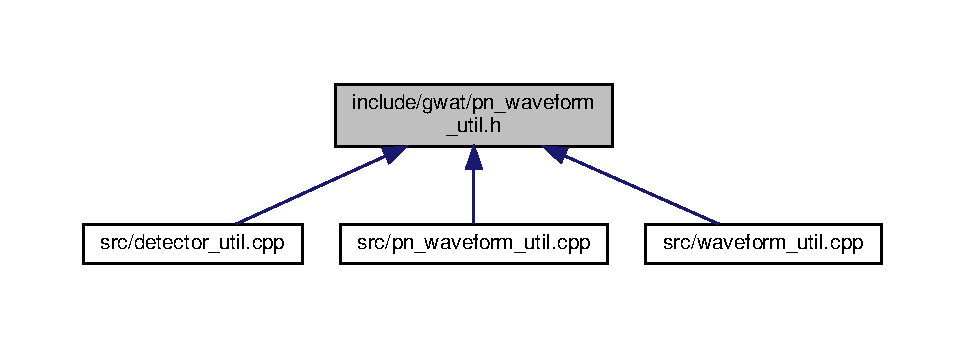
\includegraphics[width=350pt]{pn__waveform__util_8h__dep__incl}
\end{center}
\end{figure}
\doxysubsection*{Functions}
\begin{DoxyCompactItemize}
\item 
{\footnotesize template$<$class T $>$ }\\T \mbox{\hyperlink{pn__waveform__util_8h_a6ddff16ae8f9cd4b5be6d4a5d4f29c22}{t\+\_\+2\+PN}} (T f, T eta, T chirpmass, T chi1, T chi2, T tc)
\begin{DoxyCompactList}\small\item\em Time t as a function of f up to 2nd PN order. \end{DoxyCompactList}\item 
\mbox{\Hypertarget{pn__waveform__util_8h_ae592c99f579202c084ebb17e159733db}\label{pn__waveform__util_8h_ae592c99f579202c084ebb17e159733db}} 
{\footnotesize template$<$class T $>$ }\\T \mbox{\hyperlink{pn__waveform__util_8h_ae592c99f579202c084ebb17e159733db}{t\+\_\+0\+PN}} (T f, T chirpmass)
\begin{DoxyCompactList}\small\item\em Inverse of f\+\_\+0\+PN. \end{DoxyCompactList}\item 
{\footnotesize template$<$class T $>$ }\\T \mbox{\hyperlink{pn__waveform__util_8h_af5b4f8b6607df1da69fd5cfc2edad586}{f\+\_\+0\+PN}} (T t, T chirpmass)
\begin{DoxyCompactList}\small\item\em utility to get frequency from time before merger \end{DoxyCompactList}\item 
{\footnotesize template$<$class T $>$ }\\T \mbox{\hyperlink{pn__waveform__util_8h_a21c903bf96c1808515ab21865be1a082}{F\+I\+S\+CO}} (T mass)
\begin{DoxyCompactList}\small\item\em Utility function for the frequency at the innermost stable circular orbit (I\+S\+CO) \end{DoxyCompactList}\end{DoxyCompactItemize}


\doxysubsection{Detailed Description}
Header file for all P\+N-\/waveform-\/specific utilities 

\doxysubsection{Function Documentation}
\mbox{\Hypertarget{pn__waveform__util_8h_af5b4f8b6607df1da69fd5cfc2edad586}\label{pn__waveform__util_8h_af5b4f8b6607df1da69fd5cfc2edad586}} 
\index{pn\_waveform\_util.h@{pn\_waveform\_util.h}!f\_0PN@{f\_0PN}}
\index{f\_0PN@{f\_0PN}!pn\_waveform\_util.h@{pn\_waveform\_util.h}}
\doxysubsubsection{\texorpdfstring{f\_0PN()}{f\_0PN()}}
{\footnotesize\ttfamily template$<$class T $>$ \\
T f\+\_\+0\+PN (\begin{DoxyParamCaption}\item[{T}]{t,  }\item[{T}]{chirpmass }\end{DoxyParamCaption})}



utility to get frequency from time before merger 

See \href{https://arxiv.org/pdf/1902.00021.pdf}{\texttt{ https\+://arxiv.\+org/pdf/1902.\+00021.\+pdf}} \mbox{\Hypertarget{pn__waveform__util_8h_a21c903bf96c1808515ab21865be1a082}\label{pn__waveform__util_8h_a21c903bf96c1808515ab21865be1a082}} 
\index{pn\_waveform\_util.h@{pn\_waveform\_util.h}!FISCO@{FISCO}}
\index{FISCO@{FISCO}!pn\_waveform\_util.h@{pn\_waveform\_util.h}}
\doxysubsubsection{\texorpdfstring{FISCO()}{FISCO()}}
{\footnotesize\ttfamily template$<$class T $>$ \\
T F\+I\+S\+CO (\begin{DoxyParamCaption}\item[{T}]{mass }\end{DoxyParamCaption})}



Utility function for the frequency at the innermost stable circular orbit (I\+S\+CO) 

\mbox{\Hypertarget{pn__waveform__util_8h_a6ddff16ae8f9cd4b5be6d4a5d4f29c22}\label{pn__waveform__util_8h_a6ddff16ae8f9cd4b5be6d4a5d4f29c22}} 
\index{pn\_waveform\_util.h@{pn\_waveform\_util.h}!t\_2PN@{t\_2PN}}
\index{t\_2PN@{t\_2PN}!pn\_waveform\_util.h@{pn\_waveform\_util.h}}
\doxysubsubsection{\texorpdfstring{t\_2PN()}{t\_2PN()}}
{\footnotesize\ttfamily template$<$class T $>$ \\
T t\+\_\+2\+PN (\begin{DoxyParamCaption}\item[{T}]{f,  }\item[{T}]{eta,  }\item[{T}]{chirpmass,  }\item[{T}]{chi1,  }\item[{T}]{chi2,  }\item[{T}]{tc }\end{DoxyParamCaption})}



Time t as a function of f up to 2nd PN order. 

Taken from \href{https://arxiv.org/pdf/gr-qc/0411129.pdf}{\texttt{ https\+://arxiv.\+org/pdf/gr-\/qc/0411129.\+pdf}}

Non-\/precessing for now 
\hypertarget{ppE__IMRPhenomD_8h}{}\doxysection{include/gwat/pp\+E\+\_\+\+I\+M\+R\+PhenomD.h File Reference}
\label{ppE__IMRPhenomD_8h}\index{include/gwat/ppE\_IMRPhenomD.h@{include/gwat/ppE\_IMRPhenomD.h}}
{\ttfamily \#include \char`\"{}I\+M\+R\+Phenom\+D.\+h\char`\"{}}\newline
{\ttfamily \#include \char`\"{}util.\+h\char`\"{}}\newline
Include dependency graph for pp\+E\+\_\+\+I\+M\+R\+Phenom\+D.\+h\+:
% FIG 0
This graph shows which files directly or indirectly include this file\+:
% FIG 1
\doxysubsection*{Classes}
\begin{DoxyCompactItemize}
\item 
class \mbox{\hyperlink{classppE__IMRPhenomD__Inspiral}{pp\+E\+\_\+\+I\+M\+R\+Phenom\+D\+\_\+\+Inspiral$<$ T $>$}}
\item 
class \mbox{\hyperlink{classppE__IMRPhenomD__IMR}{pp\+E\+\_\+\+I\+M\+R\+Phenom\+D\+\_\+\+I\+M\+R$<$ T $>$}}
\item 
class \mbox{\hyperlink{classdCS__IMRPhenomD__log}{d\+C\+S\+\_\+\+I\+M\+R\+Phenom\+D\+\_\+log$<$ T $>$}}
\item 
class \mbox{\hyperlink{classdCS__IMRPhenomD}{d\+C\+S\+\_\+\+I\+M\+R\+Phenom\+D$<$ T $>$}}
\item 
class \mbox{\hyperlink{classEdGB__IMRPhenomD__log}{Ed\+G\+B\+\_\+\+I\+M\+R\+Phenom\+D\+\_\+log$<$ T $>$}}
\item 
class \mbox{\hyperlink{classEdGB__IMRPhenomD}{Ed\+G\+B\+\_\+\+I\+M\+R\+Phenom\+D$<$ T $>$}}
\end{DoxyCompactItemize}

\hypertarget{ppE__IMRPhenomP_8h}{}\doxysection{include/gwat/pp\+E\+\_\+\+I\+M\+R\+PhenomP.h File Reference}
\label{ppE__IMRPhenomP_8h}\index{include/gwat/ppE\_IMRPhenomP.h@{include/gwat/ppE\_IMRPhenomP.h}}
{\ttfamily \#include \char`\"{}util.\+h\char`\"{}}\newline
{\ttfamily \#include \char`\"{}I\+M\+R\+Phenom\+P.\+h\char`\"{}}\newline
Include dependency graph for pp\+E\+\_\+\+I\+M\+R\+Phenom\+P.\+h\+:
% FIG 0
This graph shows which files directly or indirectly include this file\+:
% FIG 1
\doxysubsection*{Classes}
\begin{DoxyCompactItemize}
\item 
class \mbox{\hyperlink{classppE__IMRPhenomPv2__Inspiral}{pp\+E\+\_\+\+I\+M\+R\+Phenom\+Pv2\+\_\+\+Inspiral$<$ T $>$}}
\item 
class \mbox{\hyperlink{classppE__IMRPhenomPv2__IMR}{pp\+E\+\_\+\+I\+M\+R\+Phenom\+Pv2\+\_\+\+I\+M\+R$<$ T $>$}}
\end{DoxyCompactItemize}

\hypertarget{QNM__data_8h}{}\doxysection{include/gwat/\+Q\+N\+M\+\_\+data.h File Reference}
\label{QNM__data_8h}\index{include/gwat/QNM\_data.h@{include/gwat/QNM\_data.h}}
This graph shows which files directly or indirectly include this file\+:
\nopagebreak
\begin{figure}[H]
\begin{center}
\leavevmode
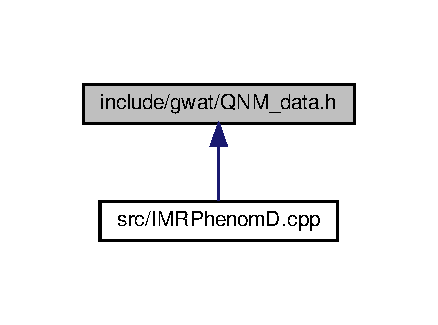
\includegraphics[width=210pt]{QNM__data_8h__dep__incl}
\end{center}
\end{figure}


\doxysubsection{Detailed Description}
Interpolation data from taken directly from L\+A\+L\+Suite

T\+O\+DO\+: Add reference to the webpage 
\hypertarget{threadPool_8h}{}\doxysection{include/gwat/thread\+Pool.h File Reference}
\label{threadPool_8h}\index{include/gwat/threadPool.h@{include/gwat/threadPool.h}}
{\ttfamily \#include $<$iostream$>$}\newline
{\ttfamily \#include $<$functional$>$}\newline
{\ttfamily \#include $<$vector$>$}\newline
{\ttfamily \#include $<$queue$>$}\newline
{\ttfamily \#include $<$thread$>$}\newline
{\ttfamily \#include $<$mutex$>$}\newline
{\ttfamily \#include $<$condition\+\_\+variable$>$}\newline
Include dependency graph for thread\+Pool.\+h\+:
% FIG 0
This graph shows which files directly or indirectly include this file\+:
% FIG 1
\doxysubsection*{Classes}
\begin{DoxyCompactItemize}
\item 
class \mbox{\hyperlink{classdefault__comp}{default\+\_\+comp$<$ jobtype $>$}}
\begin{DoxyCompactList}\small\item\em Default comparator for priority\+\_\+queue in \mbox{\hyperlink{classthreadPool}{thread\+Pool}} -- no comparison. \end{DoxyCompactList}\item 
class \mbox{\hyperlink{classthreadPool}{thread\+Pool$<$ jobtype, comparator $>$}}
\begin{DoxyCompactList}\small\item\em Class for creating a pool of threads to asynchronously distribute work. \end{DoxyCompactList}\end{DoxyCompactItemize}


\doxysubsection{Detailed Description}
Header file (declarations and definitions because of template functions) for the implementation of a generic thread pool 
\hypertarget{util_8h}{}\section{include/util.h File Reference}
\label{util_8h}\index{include/util.\+h@{include/util.\+h}}
{\ttfamily \#include $<$string$>$}\newline
{\ttfamily \#include $<$complex$>$}\newline
{\ttfamily \#include $<$adolc/adouble.\+h$>$}\newline
Include dependency graph for util.\+h\+:\nopagebreak
\begin{figure}[H]
\begin{center}
\leavevmode
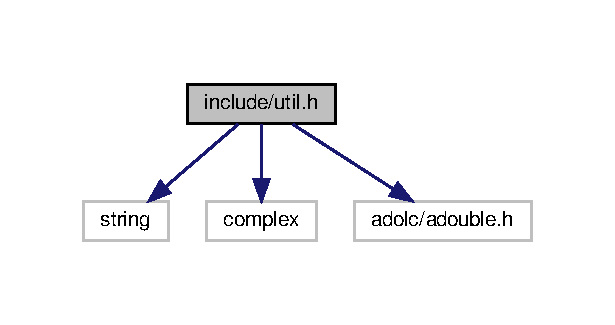
\includegraphics[width=295pt]{util_8h__incl}
\end{center}
\end{figure}
This graph shows which files directly or indirectly include this file\+:\nopagebreak
\begin{figure}[H]
\begin{center}
\leavevmode
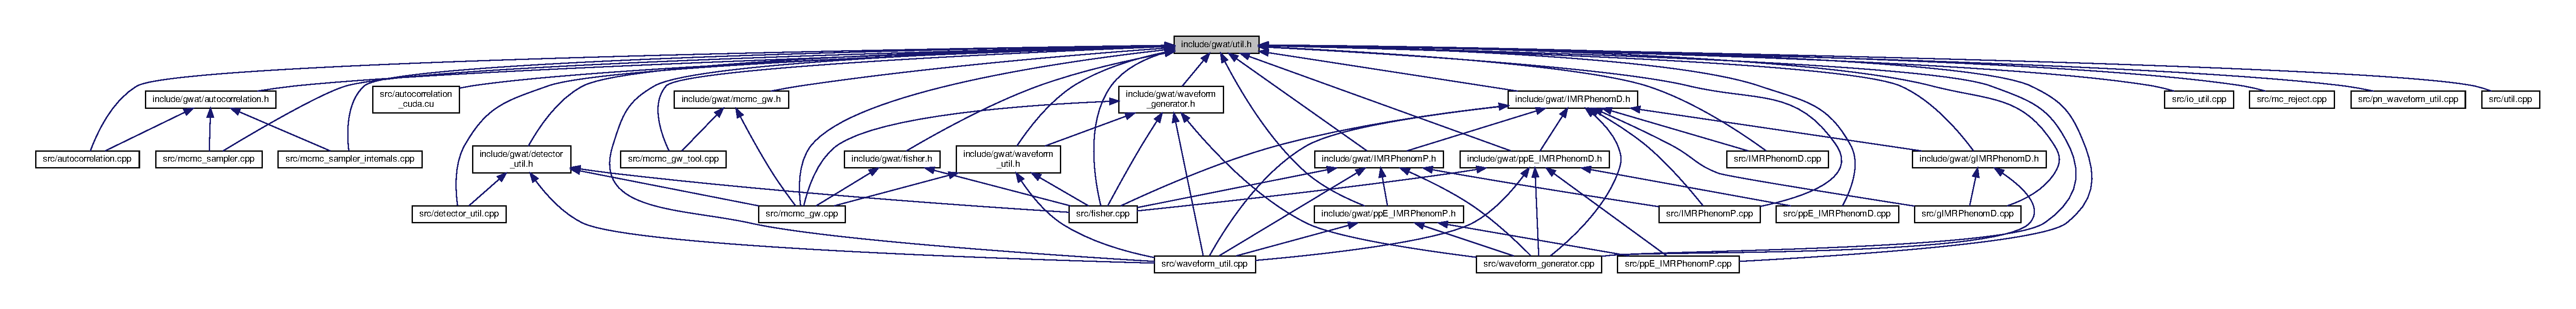
\includegraphics[width=350pt]{util_8h__dep__incl}
\end{center}
\end{figure}
\subsection*{Classes}
\begin{DoxyCompactItemize}
\item 
struct \hyperlink{structgen__params}{gen\+\_\+params}
\item 
struct \hyperlink{structuseful__powers}{useful\+\_\+powers$<$ T $>$}
\begin{DoxyCompactList}\small\item\em To speed up calculations within the for loops, we pre-\/calculate reoccuring powers of M$\ast$F and Pi, since the pow() function is prohibatively slow. \end{DoxyCompactList}\item 
struct \hyperlink{structsource__parameters}{source\+\_\+parameters$<$ T $>$}
\end{DoxyCompactItemize}
\subsection*{Functions}
\begin{DoxyCompactItemize}
\item 
\mbox{\Hypertarget{util_8h_a06ffbad5fe4daa3872db626f90556202}\label{util_8h_a06ffbad5fe4daa3872db626f90556202}} 
double \hyperlink{util_8h_a06ffbad5fe4daa3872db626f90556202}{calculate\+\_\+eta} (double mass1, double mass2)
\begin{DoxyCompactList}\small\item\em Calculates the symmetric mass ration from the two component masses. \end{DoxyCompactList}\item 
\mbox{\Hypertarget{util_8h_adc4391c722f94cb17f0e0275a0930fa9}\label{util_8h_adc4391c722f94cb17f0e0275a0930fa9}} 
adouble {\bfseries calculate\+\_\+eta} (adouble mass1, adouble mass2)
\item 
double \hyperlink{util_8h_af7aeeebcf190ab70c667a478a51ce435}{calculate\+\_\+chirpmass} (double mass1, double mass2)
\begin{DoxyCompactList}\small\item\em Calculates the chirp mass from the two component masses. \end{DoxyCompactList}\item 
\mbox{\Hypertarget{util_8h_a0a7a0da86013d639bf8689c9a01d8583}\label{util_8h_a0a7a0da86013d639bf8689c9a01d8583}} 
adouble {\bfseries calculate\+\_\+chirpmass} (adouble mass1, adouble mass2)
\item 
double \hyperlink{util_8h_a85a0fc50a6f06dd519a18a6d273a0b4a}{calculate\+\_\+mass1} (double chirpmass, double eta)
\begin{DoxyCompactList}\small\item\em Calculates the larger mass given a chirp mass and symmetric mass ratio. \end{DoxyCompactList}\item 
\mbox{\Hypertarget{util_8h_a663f11702648d9a84c9b573e9ab76f09}\label{util_8h_a663f11702648d9a84c9b573e9ab76f09}} 
adouble {\bfseries calculate\+\_\+mass1} (adouble chirpmass, adouble eta)
\item 
double \hyperlink{util_8h_a5f62f4a7c1011180080d72e0032cef1b}{calculate\+\_\+mass2} (double chirpmass, double eta)
\begin{DoxyCompactList}\small\item\em Calculates the smaller mass given a chirp mass and symmetric mass ratio. \end{DoxyCompactList}\item 
\mbox{\Hypertarget{util_8h_adb85ce9fbb2e3a438dd41a35c38a3237}\label{util_8h_adb85ce9fbb2e3a438dd41a35c38a3237}} 
adouble {\bfseries calculate\+\_\+mass2} (adouble chirpmass, adouble eta)
\item 
{\footnotesize template$<$class T $>$ }\\T \hyperlink{util_8h_a185f5ce6420f94f03d77915d94b06f4f}{trapezoidal\+\_\+sum\+\_\+uniform} (double delta\+\_\+x, int length, T $\ast$integrand)
\begin{DoxyCompactList}\small\item\em Trapezoidal sum rule to approximate discrete integral -\/ Uniform spacing. \end{DoxyCompactList}\item 
{\footnotesize template$<$class T $>$ }\\T \hyperlink{util_8h_ab7d3ff0c020ec0ffbe56f4271f425d68}{trapezoidal\+\_\+sum} (double $\ast$delta\+\_\+x, int length, T $\ast$integrand)
\begin{DoxyCompactList}\small\item\em Trapezoidal sum rule to approximate discrete integral -\/ Non-\/\+Uniform spacing. \end{DoxyCompactList}\item 
{\footnotesize template$<$class T $>$ }\\T \hyperlink{util_8h_ad77170ec9220ef33a32f2540e9184e31}{simpsons\+\_\+sum} (double delta\+\_\+x, int length, T $\ast$integrand)
\begin{DoxyCompactList}\small\item\em Simpsons sum rule to approximate discrete integral -\/ Uniform spacing. \end{DoxyCompactList}\item 
\mbox{\Hypertarget{util_8h_ae40cc3f267c33745a8a2485638d5db55}\label{util_8h_ae40cc3f267c33745a8a2485638d5db55}} 
long {\bfseries factorial} (long num)
\end{DoxyCompactItemize}
\subsection*{Variables}
\begin{DoxyCompactItemize}
\item 
const double \hyperlink{util_8h_ae35ccfea47f0da0a31cf1d13c80f3c58}{gamma\+\_\+E} = 0.\+5772156649015328606065120900824024310421
\item 
const double \hyperlink{util_8h_a8fc6defe4e499b1b9b9c275689e44352}{c} = 299792458.
\item 
const double \hyperlink{util_8h_ab97e4616d23ed4c2961295010c1afc3c}{G} =6.\+674e-\/11$\ast$(1.\+98855e30)
\item 
const double \hyperlink{util_8h_a498f9210d23417e309c01ad5cb9a635b}{M\+S\+O\+L\+\_\+\+S\+EC} =492549095.e-\/14
\item 
const double \hyperlink{util_8h_a47be806b6c8a58bd030f167ca91ed201}{M\+P\+C\+\_\+\+S\+EC} = 3085677581.e13/\hyperlink{util_8h_a8fc6defe4e499b1b9b9c275689e44352}{c}
\end{DoxyCompactItemize}


\subsection{Detailed Description}
General utilities (functions and structures) independent of modelling method 

\subsection{Function Documentation}
\mbox{\Hypertarget{util_8h_af7aeeebcf190ab70c667a478a51ce435}\label{util_8h_af7aeeebcf190ab70c667a478a51ce435}} 
\index{util.\+h@{util.\+h}!calculate\+\_\+chirpmass@{calculate\+\_\+chirpmass}}
\index{calculate\+\_\+chirpmass@{calculate\+\_\+chirpmass}!util.\+h@{util.\+h}}
\subsubsection{\texorpdfstring{calculate\+\_\+chirpmass()}{calculate\_chirpmass()}}
{\footnotesize\ttfamily double calculate\+\_\+chirpmass (\begin{DoxyParamCaption}\item[{double}]{mass1,  }\item[{double}]{mass2 }\end{DoxyParamCaption})}



Calculates the chirp mass from the two component masses. 

The output units are whatever units the input masses are \mbox{\Hypertarget{util_8h_a85a0fc50a6f06dd519a18a6d273a0b4a}\label{util_8h_a85a0fc50a6f06dd519a18a6d273a0b4a}} 
\index{util.\+h@{util.\+h}!calculate\+\_\+mass1@{calculate\+\_\+mass1}}
\index{calculate\+\_\+mass1@{calculate\+\_\+mass1}!util.\+h@{util.\+h}}
\subsubsection{\texorpdfstring{calculate\+\_\+mass1()}{calculate\_mass1()}}
{\footnotesize\ttfamily double calculate\+\_\+mass1 (\begin{DoxyParamCaption}\item[{double}]{chirpmass,  }\item[{double}]{eta }\end{DoxyParamCaption})}



Calculates the larger mass given a chirp mass and symmetric mass ratio. 

Units of the output match the units of the input chirp mass \mbox{\Hypertarget{util_8h_a5f62f4a7c1011180080d72e0032cef1b}\label{util_8h_a5f62f4a7c1011180080d72e0032cef1b}} 
\index{util.\+h@{util.\+h}!calculate\+\_\+mass2@{calculate\+\_\+mass2}}
\index{calculate\+\_\+mass2@{calculate\+\_\+mass2}!util.\+h@{util.\+h}}
\subsubsection{\texorpdfstring{calculate\+\_\+mass2()}{calculate\_mass2()}}
{\footnotesize\ttfamily double calculate\+\_\+mass2 (\begin{DoxyParamCaption}\item[{double}]{chirpmass,  }\item[{double}]{eta }\end{DoxyParamCaption})}



Calculates the smaller mass given a chirp mass and symmetric mass ratio. 

Units of the output match the units of the input chirp mass \mbox{\Hypertarget{util_8h_ad77170ec9220ef33a32f2540e9184e31}\label{util_8h_ad77170ec9220ef33a32f2540e9184e31}} 
\index{util.\+h@{util.\+h}!simpsons\+\_\+sum@{simpsons\+\_\+sum}}
\index{simpsons\+\_\+sum@{simpsons\+\_\+sum}!util.\+h@{util.\+h}}
\subsubsection{\texorpdfstring{simpsons\+\_\+sum()}{simpsons\_sum()}}
{\footnotesize\ttfamily template$<$class T $>$ \\
T simpsons\+\_\+sum (\begin{DoxyParamCaption}\item[{double}]{delta\+\_\+x,  }\item[{int}]{length,  }\item[{T $\ast$}]{integrand }\end{DoxyParamCaption})}



Simpsons sum rule to approximate discrete integral -\/ Uniform spacing. 

More accurate than the trapezoidal rule, but must be uniform \mbox{\Hypertarget{util_8h_ab7d3ff0c020ec0ffbe56f4271f425d68}\label{util_8h_ab7d3ff0c020ec0ffbe56f4271f425d68}} 
\index{util.\+h@{util.\+h}!trapezoidal\+\_\+sum@{trapezoidal\+\_\+sum}}
\index{trapezoidal\+\_\+sum@{trapezoidal\+\_\+sum}!util.\+h@{util.\+h}}
\subsubsection{\texorpdfstring{trapezoidal\+\_\+sum()}{trapezoidal\_sum()}}
{\footnotesize\ttfamily template$<$class T $>$ \\
T trapezoidal\+\_\+sum (\begin{DoxyParamCaption}\item[{double $\ast$}]{delta\+\_\+x,  }\item[{int}]{length,  }\item[{T $\ast$}]{integrand }\end{DoxyParamCaption})}



Trapezoidal sum rule to approximate discrete integral -\/ Non-\/\+Uniform spacing. 

This version is slower than the uniform version, but will handle non-\/uniform spacing \mbox{\Hypertarget{util_8h_a185f5ce6420f94f03d77915d94b06f4f}\label{util_8h_a185f5ce6420f94f03d77915d94b06f4f}} 
\index{util.\+h@{util.\+h}!trapezoidal\+\_\+sum\+\_\+uniform@{trapezoidal\+\_\+sum\+\_\+uniform}}
\index{trapezoidal\+\_\+sum\+\_\+uniform@{trapezoidal\+\_\+sum\+\_\+uniform}!util.\+h@{util.\+h}}
\subsubsection{\texorpdfstring{trapezoidal\+\_\+sum\+\_\+uniform()}{trapezoidal\_sum\_uniform()}}
{\footnotesize\ttfamily template$<$class T $>$ \\
T trapezoidal\+\_\+sum\+\_\+uniform (\begin{DoxyParamCaption}\item[{double}]{delta\+\_\+x,  }\item[{int}]{length,  }\item[{T $\ast$}]{integrand }\end{DoxyParamCaption})}



Trapezoidal sum rule to approximate discrete integral -\/ Uniform spacing. 

This version is faster than the general version, as it has half the function calls

Something may be wrong with this function -\/ had an overall offset for real data that was fixed by using the simpsons rule -\/ not sure if this was because of a boost in accuracy or because something is off with the trapezoidal sum 

\subsection{Variable Documentation}
\mbox{\Hypertarget{util_8h_a8fc6defe4e499b1b9b9c275689e44352}\label{util_8h_a8fc6defe4e499b1b9b9c275689e44352}} 
\index{util.\+h@{util.\+h}!c@{c}}
\index{c@{c}!util.\+h@{util.\+h}}
\subsubsection{\texorpdfstring{c}{c}}
{\footnotesize\ttfamily const double c = 299792458.}

Speed of light m/s \mbox{\Hypertarget{util_8h_ab97e4616d23ed4c2961295010c1afc3c}\label{util_8h_ab97e4616d23ed4c2961295010c1afc3c}} 
\index{util.\+h@{util.\+h}!G@{G}}
\index{G@{G}!util.\+h@{util.\+h}}
\subsubsection{\texorpdfstring{G}{G}}
{\footnotesize\ttfamily const double G =6.\+674e-\/11$\ast$(1.\+98855e30)}

Gravitational constant in m$\ast$$\ast$3/(s$\ast$$\ast$2 Sol\+Mass) \mbox{\Hypertarget{util_8h_ae35ccfea47f0da0a31cf1d13c80f3c58}\label{util_8h_ae35ccfea47f0da0a31cf1d13c80f3c58}} 
\index{util.\+h@{util.\+h}!gamma\+\_\+E@{gamma\+\_\+E}}
\index{gamma\+\_\+E@{gamma\+\_\+E}!util.\+h@{util.\+h}}
\subsubsection{\texorpdfstring{gamma\+\_\+E}{gamma\_E}}
{\footnotesize\ttfamily const double gamma\+\_\+E = 0.\+5772156649015328606065120900824024310421}

Euler number \mbox{\Hypertarget{util_8h_a47be806b6c8a58bd030f167ca91ed201}\label{util_8h_a47be806b6c8a58bd030f167ca91ed201}} 
\index{util.\+h@{util.\+h}!M\+P\+C\+\_\+\+S\+EC@{M\+P\+C\+\_\+\+S\+EC}}
\index{M\+P\+C\+\_\+\+S\+EC@{M\+P\+C\+\_\+\+S\+EC}!util.\+h@{util.\+h}}
\subsubsection{\texorpdfstring{M\+P\+C\+\_\+\+S\+EC}{MPC\_SEC}}
{\footnotesize\ttfamily const double M\+P\+C\+\_\+\+S\+EC = 3085677581.e13/\hyperlink{util_8h_a8fc6defe4e499b1b9b9c275689e44352}{c}}

consts.\+kpc.\+to(\textquotesingle{}m\textquotesingle{})$\ast$1000/c Mpc in sec \mbox{\Hypertarget{util_8h_a498f9210d23417e309c01ad5cb9a635b}\label{util_8h_a498f9210d23417e309c01ad5cb9a635b}} 
\index{util.\+h@{util.\+h}!M\+S\+O\+L\+\_\+\+S\+EC@{M\+S\+O\+L\+\_\+\+S\+EC}}
\index{M\+S\+O\+L\+\_\+\+S\+EC@{M\+S\+O\+L\+\_\+\+S\+EC}!util.\+h@{util.\+h}}
\subsubsection{\texorpdfstring{M\+S\+O\+L\+\_\+\+S\+EC}{MSOL\_SEC}}
{\footnotesize\ttfamily const double M\+S\+O\+L\+\_\+\+S\+EC =492549095.e-\/14}

G/c$\ast$$\ast$3 seconds per solar mass 
\hypertarget{waveform__generator_8h}{}\doxysection{include/gwat/waveform\+\_\+generator.h File Reference}
\label{waveform__generator_8h}\index{include/gwat/waveform\_generator.h@{include/gwat/waveform\_generator.h}}
{\ttfamily \#include $<$math.\+h$>$}\newline
{\ttfamily \#include \char`\"{}util.\+h\char`\"{}}\newline
{\ttfamily \#include $<$complex$>$}\newline
{\ttfamily \#include $<$string$>$}\newline
Include dependency graph for waveform\+\_\+generator.\+h\+:
\nopagebreak
\begin{figure}[H]
\begin{center}
\leavevmode
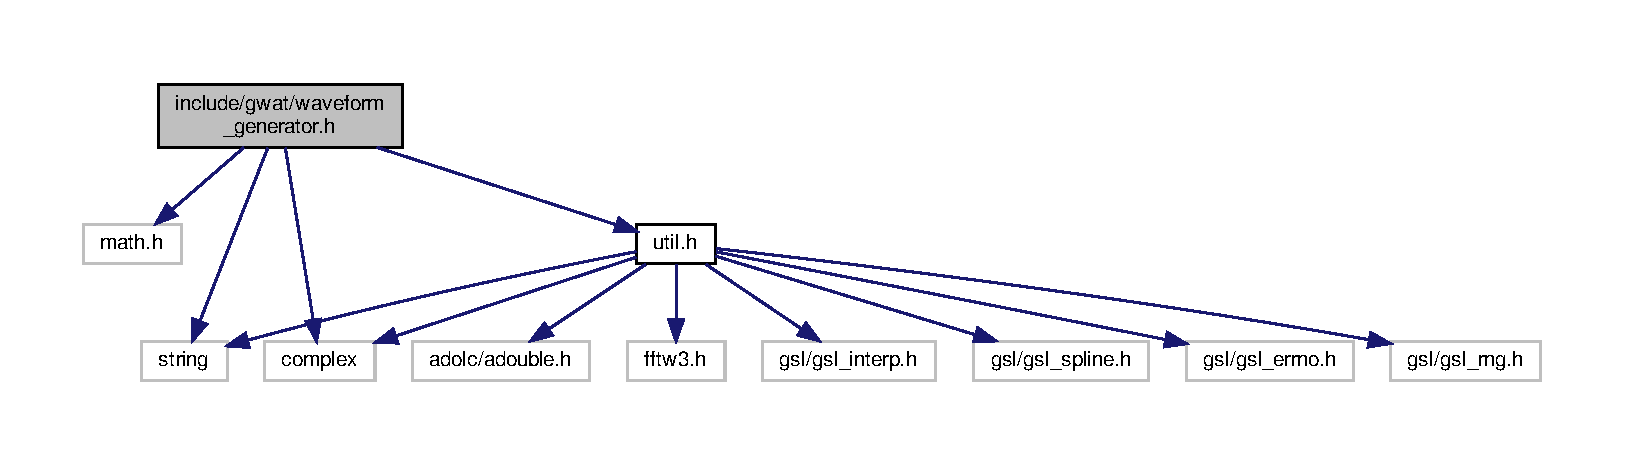
\includegraphics[width=350pt]{waveform__generator_8h__incl}
\end{center}
\end{figure}
This graph shows which files directly or indirectly include this file\+:
\nopagebreak
\begin{figure}[H]
\begin{center}
\leavevmode
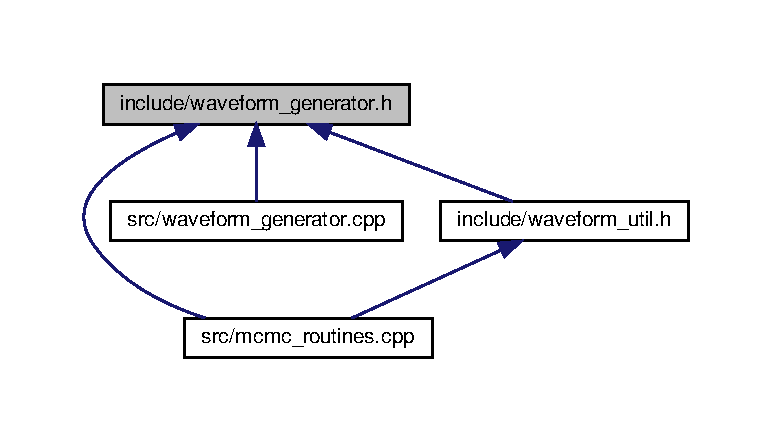
\includegraphics[width=350pt]{waveform__generator_8h__dep__incl}
\end{center}
\end{figure}
\doxysubsection*{Functions}
\begin{DoxyCompactItemize}
\item 
\mbox{\Hypertarget{waveform__generator_8h_a06574718b86529ab0480a6a673ada3f6}\label{waveform__generator_8h_a06574718b86529ab0480a6a673ada3f6}} 
{\footnotesize template$<$class T $>$ }\\int {\bfseries fourier\+\_\+waveform} (T $\ast$frequencies, int length, std\+::complex$<$ T $>$ $\ast$waveform\+\_\+plus, std\+::complex$<$ T $>$ $\ast$waveform\+\_\+cross, std\+::string generation\+\_\+method, \mbox{\hyperlink{classgen__params__base}{gen\+\_\+params\+\_\+base}}$<$ T $>$ $\ast$parameters)
\item 
\mbox{\Hypertarget{waveform__generator_8h_aab7ecf30458b3577aa1391c464bbe671}\label{waveform__generator_8h_aab7ecf30458b3577aa1391c464bbe671}} 
int {\bfseries fourier\+\_\+waveform} (double $\ast$frequencies, int length, double $\ast$waveform\+\_\+plus\+\_\+real, double $\ast$waveform\+\_\+plus\+\_\+imag, double $\ast$waveform\+\_\+cross\+\_\+real, double $\ast$waveform\+\_\+cross\+\_\+imag, std\+::string generation\+\_\+method, \mbox{\hyperlink{classgen__params}{gen\+\_\+params}} $\ast$parameters)
\item 
\mbox{\Hypertarget{waveform__generator_8h_ace521e7a8e3747632121ceabf6eaa305}\label{waveform__generator_8h_ace521e7a8e3747632121ceabf6eaa305}} 
int {\bfseries fourier\+\_\+waveform} (double $\ast$frequencies, int length, std\+::complex$<$ double $>$ $\ast$waveform, std\+::string generation\+\_\+method, \mbox{\hyperlink{classgen__params}{gen\+\_\+params}} $\ast$parameters)
\item 
\mbox{\Hypertarget{waveform__generator_8h_a3f551caee9adc33674e4b74daa6bbb54}\label{waveform__generator_8h_a3f551caee9adc33674e4b74daa6bbb54}} 
int {\bfseries fourier\+\_\+waveform} (double $\ast$frequencies, int length, double $\ast$waveform\+\_\+real, double $\ast$waveform\+\_\+imag, std\+::string generation\+\_\+method, \mbox{\hyperlink{classgen__params}{gen\+\_\+params}} $\ast$parameters)
\item 
\mbox{\Hypertarget{waveform__generator_8h_a0c791c00bc1552f2f70cadfbdff73a06}\label{waveform__generator_8h_a0c791c00bc1552f2f70cadfbdff73a06}} 
{\footnotesize template$<$class T $>$ }\\int {\bfseries fourier\+\_\+amplitude} (T $\ast$frequencies, int length, T $\ast$amplitude, std\+::string generation\+\_\+method, \mbox{\hyperlink{classgen__params__base}{gen\+\_\+params\+\_\+base}}$<$ T $>$ $\ast$parameters)
\item 
\mbox{\Hypertarget{waveform__generator_8h_a68aef1d43c5333493d165d32b6f11685}\label{waveform__generator_8h_a68aef1d43c5333493d165d32b6f11685}} 
{\footnotesize template$<$class T $>$ }\\int {\bfseries fourier\+\_\+phase} (T $\ast$frequencies, int length, T $\ast$phase, std\+::string generation\+\_\+method, \mbox{\hyperlink{classgen__params__base}{gen\+\_\+params\+\_\+base}}$<$ T $>$ $\ast$parameters)
\item 
\mbox{\Hypertarget{waveform__generator_8h_ae0fa91d4261e2c39116cf2be47fd5724}\label{waveform__generator_8h_ae0fa91d4261e2c39116cf2be47fd5724}} 
{\footnotesize template$<$class T $>$ }\\int {\bfseries fourier\+\_\+phase} (T $\ast$frequencies, int length, T $\ast$phase\+\_\+plus, T $\ast$phase\+\_\+cross, std\+::string generation\+\_\+method, \mbox{\hyperlink{classgen__params__base}{gen\+\_\+params\+\_\+base}}$<$ T $>$ $\ast$parameters)
\end{DoxyCompactItemize}

\hypertarget{waveform__generator__C_8h}{}\doxysection{include/gwat/waveform\+\_\+generator\+\_\+C.h File Reference}
\label{waveform__generator__C_8h}\index{include/gwat/waveform\_generator\_C.h@{include/gwat/waveform\_generator\_C.h}}
\doxysubsection*{Functions}
\begin{DoxyCompactItemize}
\item 
\mbox{\Hypertarget{waveform__generator__C_8h_ae8af533450c96ef8034d982b7645fc94}\label{waveform__generator__C_8h_ae8af533450c96ef8034d982b7645fc94}} 
int {\bfseries fourier\+\_\+waveformC} (double $\ast$frequencies, int length, double $\ast$waveform\+\_\+plus\+\_\+real, double $\ast$waveform\+\_\+plus\+\_\+imag, double $\ast$waveform\+\_\+cross\+\_\+real, double $\ast$waveform\+\_\+cross\+\_\+imag, char $\ast$generation\+\_\+method, double mass1, double mass2, double DL, double spin1x, double spin1y, double spin1z, double spin2x, double spin2y, double spin2z, double phic, double tc, double f\+\_\+ref, double phi\+Ref, double $\ast$pp\+E\+\_\+beta, int $\ast$pp\+E\+\_\+b, int Nmod, double incl\+\_\+angle, double theta, double phi)
\item 
\mbox{\Hypertarget{waveform__generator__C_8h_a18c1264b84b1be0ffdae4e08e4965435}\label{waveform__generator__C_8h_a18c1264b84b1be0ffdae4e08e4965435}} 
int {\bfseries fourier\+\_\+amplitudeC} (double $\ast$frequencies, int length, double $\ast$amplitude, char $\ast$generation\+\_\+method, double mass1, double mass2, double DL, double spin1x, double spin1y, double spin1z, double spin2x, double spin2y, double spin2z, double incl\+\_\+angle, double theta, double phi)
\item 
\mbox{\Hypertarget{waveform__generator__C_8h_a341b2b488fa3011145bcdeaeceb49db7}\label{waveform__generator__C_8h_a341b2b488fa3011145bcdeaeceb49db7}} 
int {\bfseries fourier\+\_\+phaseC} (double $\ast$frequencies, int length, double $\ast$phase, char $\ast$generation\+\_\+method, double mass1, double mass2, double DL, double spin1x, double spin1y, double spin1z, double spin2x, double spin2y, double spin2z, double phic, double tc, double f\+\_\+ref, double phi\+Ref, double $\ast$pp\+E\+\_\+beta, int $\ast$pp\+E\+\_\+b, int Nmod, double incl\+\_\+angle, double theta, double phi)
\item 
\mbox{\Hypertarget{waveform__generator__C_8h_af0c1c7d52a5ce245b593c2925413895d}\label{waveform__generator__C_8h_af0c1c7d52a5ce245b593c2925413895d}} 
void {\bfseries initiate\+\_\+\+Lum\+D\+\_\+\+Z\+\_\+interp\+\_\+C} ()
\item 
\mbox{\Hypertarget{waveform__generator__C_8h_ab483270374d434fb6ce50afc456578d7}\label{waveform__generator__C_8h_ab483270374d434fb6ce50afc456578d7}} 
void {\bfseries free\+\_\+\+Lum\+D\+\_\+\+Z\+\_\+interp\+\_\+C} ()
\end{DoxyCompactItemize}


\doxysubsection{Detailed Description}
Header file for the C wrapping of the waveform\+\_\+generation.\+cpp 
\hypertarget{waveform__util_8h}{}\doxysection{include/gwat/waveform\+\_\+util.h File Reference}
\label{waveform__util_8h}\index{include/gwat/waveform\_util.h@{include/gwat/waveform\_util.h}}
{\ttfamily \#include \char`\"{}waveform\+\_\+generator.\+h\char`\"{}}\newline
{\ttfamily \#include \char`\"{}util.\+h\char`\"{}}\newline
{\ttfamily \#include $<$string$>$}\newline
{\ttfamily \#include $<$gsl/gsl\+\_\+integration.\+h$>$}\newline
Include dependency graph for waveform\+\_\+util.\+h\+:
\nopagebreak
\begin{figure}[H]
\begin{center}
\leavevmode
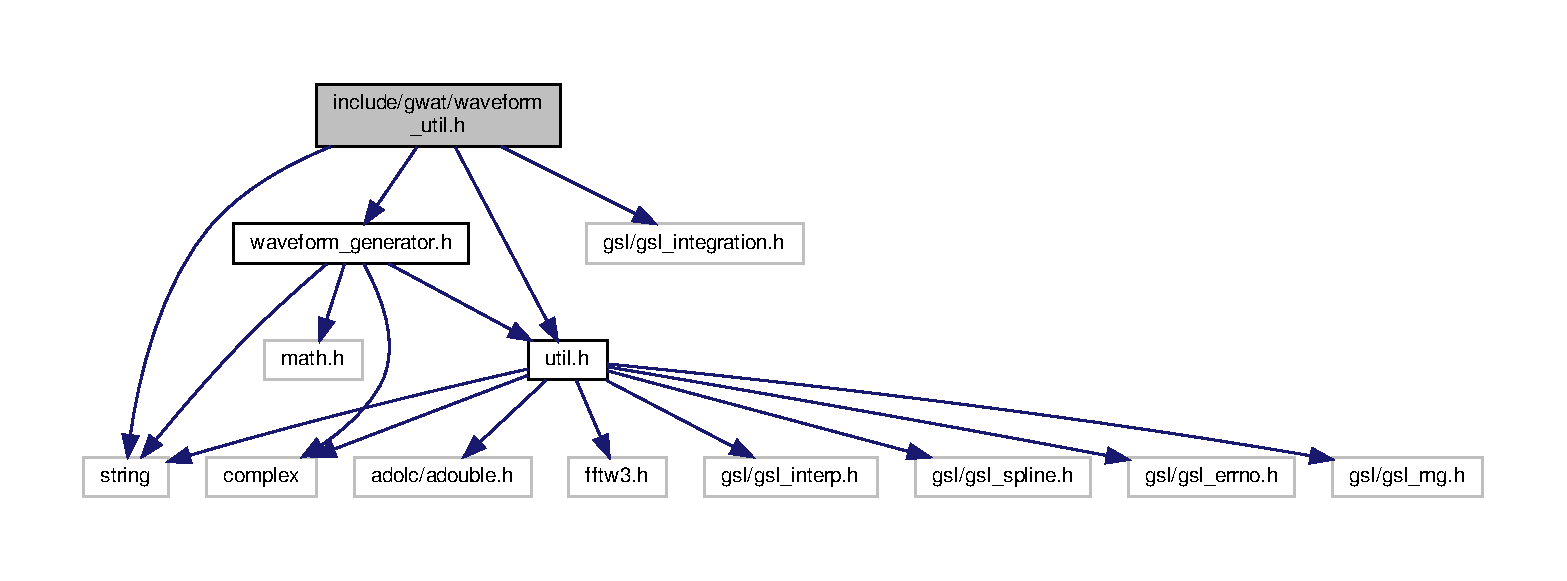
\includegraphics[width=350pt]{waveform__util_8h__incl}
\end{center}
\end{figure}
This graph shows which files directly or indirectly include this file\+:
\nopagebreak
\begin{figure}[H]
\begin{center}
\leavevmode
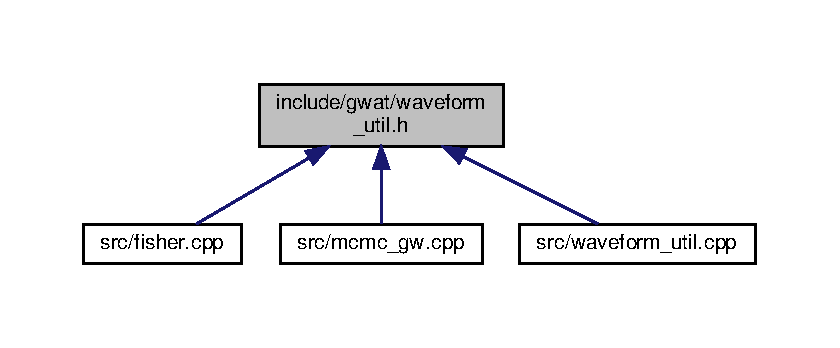
\includegraphics[width=350pt]{waveform__util_8h__dep__incl}
\end{center}
\end{figure}
\doxysubsection*{Functions}
\begin{DoxyCompactItemize}
\item 
double \mbox{\hyperlink{waveform__util_8h_a0a5e9bfac97929ed68c247c3ff90fca2}{data\+\_\+snr\+\_\+maximized\+\_\+extrinsic}} (double $\ast$frequencies, int length, std\+::complex$<$ double $>$ $\ast$data, double $\ast$psd, std\+::string detector, std\+::string generation\+\_\+method, \mbox{\hyperlink{classgen__params}{gen\+\_\+params}} $\ast$param)
\begin{DoxyCompactList}\small\item\em Utility to calculate the snr of a fourier transformed data stream while maximizing over the coalescence parameters phic and tc. \end{DoxyCompactList}\item 
double \mbox{\hyperlink{waveform__util_8h_a85abee44a54e906762d980f56b76bc46}{data\+\_\+snr\+\_\+maximized\+\_\+extrinsic}} (double $\ast$frequencies, int length, double $\ast$data\+\_\+real, double $\ast$data\+\_\+imag, double $\ast$psd, std\+::string detector, std\+::string generation\+\_\+method, \mbox{\hyperlink{classgen__params}{gen\+\_\+params}} $\ast$param)
\begin{DoxyCompactList}\small\item\em Light wrapper for the data\+\_\+snr\+\_\+maximized\+\_\+extrinsic method. \end{DoxyCompactList}\item 
double \mbox{\hyperlink{waveform__util_8h_a65e74aae0c49a3854f81e349413b20e5}{calculate\+\_\+snr}} (std\+::string sensitivity\+\_\+curve, std\+::complex$<$ double $>$ $\ast$waveform, double $\ast$frequencies, int length)
\begin{DoxyCompactList}\small\item\em Caclulates the snr given a detector and waveform (complex) and frequencies. \end{DoxyCompactList}\item 
\mbox{\Hypertarget{waveform__util_8h_a6e923c1ceedf04aab52a9635a67e2aa2}\label{waveform__util_8h_a6e923c1ceedf04aab52a9635a67e2aa2}} 
double {\bfseries calculate\+\_\+snr\+\_\+internal} (double $\ast$psd, std\+::complex$<$ double $>$ $\ast$waveform, double $\ast$frequencies, int length)
\item 
double \mbox{\hyperlink{waveform__util_8h_a24123fc7426785f73e4b393af556e3b2}{calculate\+\_\+snr}} (std\+::string sensitivity\+\_\+curve, std\+::string detector, std\+::string generation\+\_\+method, \mbox{\hyperlink{classgen__params__base}{gen\+\_\+params\+\_\+base}}$<$ double $>$ $\ast$params, double $\ast$frequencies, int length)
\begin{DoxyCompactList}\small\item\em Routine to calculate the S\+NR of a template with G\+SL quadrature integration. \end{DoxyCompactList}\item 
int \mbox{\hyperlink{waveform__util_8h_ae457f376ac6868d88fa7c428a1cc0798}{calculate\+\_\+snr\+\_\+gsl}} (double $\ast$snr, std\+::string sensitivity\+\_\+curve, std\+::string detector, std\+::string generation\+\_\+method, \mbox{\hyperlink{classgen__params__base}{gen\+\_\+params\+\_\+base}}$<$ double $>$ $\ast$params, double f\+\_\+min, double f\+\_\+max, double relative\+\_\+error)
\begin{DoxyCompactList}\small\item\em Routine to calculate the S\+NR of a template with G\+SL quadrature integration. \end{DoxyCompactList}\item 
int \mbox{\hyperlink{waveform__util_8h_a7a6b3d3d9c2f2fee67faef89f435f780}{calculate\+\_\+snr\+\_\+gsl}} (double $\ast$snr, std\+::string sensitivity\+\_\+curve, std\+::string detector, std\+::string generation\+\_\+method, \mbox{\hyperlink{classgen__params__base}{gen\+\_\+params\+\_\+base}}$<$ double $>$ $\ast$params, double f\+\_\+min, double f\+\_\+max, double relative\+\_\+error, gsl\+\_\+integration\+\_\+workspace $\ast$w, int np)
\item 
\mbox{\Hypertarget{waveform__util_8h_aac4a9bc1f23ef60f44b6497cbc0a1c62}\label{waveform__util_8h_aac4a9bc1f23ef60f44b6497cbc0a1c62}} 
double \mbox{\hyperlink{waveform__util_8h_aac4a9bc1f23ef60f44b6497cbc0a1c62}{integrand\+\_\+snr\+\_\+\+S\+A\+\_\+subroutine}} (double f, void $\ast$subroutine\+\_\+params)
\begin{DoxyCompactList}\small\item\em Internal function to calculate the S\+NR integrand for sky-\/averaged waveforms. \end{DoxyCompactList}\item 
\mbox{\Hypertarget{waveform__util_8h_a61996edcf8006475f688ef5ab6a22be8}\label{waveform__util_8h_a61996edcf8006475f688ef5ab6a22be8}} 
double \mbox{\hyperlink{waveform__util_8h_a61996edcf8006475f688ef5ab6a22be8}{integrand\+\_\+snr\+\_\+subroutine}} (double f, void $\ast$subroutine\+\_\+params)
\begin{DoxyCompactList}\small\item\em Internal function to calculate the S\+NR integrand for full waveforms. \end{DoxyCompactList}\item 
{\footnotesize template$<$class T $>$ }\\int \mbox{\hyperlink{waveform__util_8h_acfc4f9ff901f2b97fe3c90464eaf6ddd}{fourier\+\_\+detector\+\_\+response\+\_\+horizon}} (T $\ast$frequencies, int length, std\+::complex$<$ T $>$ $\ast$hplus, std\+::complex$<$ T $>$ $\ast$hcross, std\+::complex$<$ T $>$ $\ast$detector\+\_\+response, T theta, T phi, std\+::string detector)
\item 
{\footnotesize template$<$class T $>$ }\\int \mbox{\hyperlink{waveform__util_8h_a46e4717d9625b9ab1f288934628a152f}{fourier\+\_\+detector\+\_\+response\+\_\+horizon}} (T $\ast$frequencies, int length, std\+::complex$<$ T $>$ $\ast$hplus, std\+::complex$<$ T $>$ $\ast$hcross, std\+::complex$<$ T $>$ $\ast$detector\+\_\+response, T theta, T phi, T psi, std\+::string detector)
\item 
{\footnotesize template$<$class T $>$ }\\int \mbox{\hyperlink{waveform__util_8h_ada5544fbdbe68fb348d59fa7714fa35e}{fourier\+\_\+detector\+\_\+response\+\_\+horizon}} (T $\ast$frequencies, int length, std\+::complex$<$ T $>$ $\ast$response, std\+::string detector, std\+::string generation\+\_\+method, \mbox{\hyperlink{classgen__params__base}{gen\+\_\+params\+\_\+base}}$<$ T $>$ $\ast$parameters)
\begin{DoxyCompactList}\small\item\em Function to produce the detector response caused by impinging gravitational waves from a quasi-\/circular binary. \end{DoxyCompactList}\item 
{\footnotesize template$<$class T $>$ }\\int \mbox{\hyperlink{waveform__util_8h_ad3e4a354390ac1f31d58d4cbd1090e25}{fourier\+\_\+detector\+\_\+response\+\_\+equatorial}} (T $\ast$frequencies, int length, std\+::complex$<$ T $>$ $\ast$hplus, std\+::complex$<$ T $>$ $\ast$hcross, std\+::complex$<$ T $>$ $\ast$detector\+\_\+response, T ra, T dec, T psi, double gmst, T $\ast$times, T L\+I\+S\+A\+\_\+alpha0, T L\+I\+S\+A\+\_\+phi0, T theta\+\_\+j\+\_\+ecl, T phi\+\_\+j\+\_\+ecl, std\+::string detector)
\item 
{\footnotesize template$<$class T $>$ }\\int \mbox{\hyperlink{waveform__util_8h_a234c1a71c579c913e0c1033d951dbbe5}{fourier\+\_\+detector\+\_\+response\+\_\+equatorial}} (T $\ast$frequencies, int length, std\+::complex$<$ T $>$ $\ast$response, std\+::string detector, std\+::string generation\+\_\+method, \mbox{\hyperlink{classgen__params__base}{gen\+\_\+params\+\_\+base}}$<$ T $>$ $\ast$parameters)
\begin{DoxyCompactList}\small\item\em Function to produce the detector response caused by impinging gravitational waves from a quasi-\/circular binary for equatorial coordinates for T\+E\+R\+R\+E\+S\+T\+I\+AL detectors, where the earth\textquotesingle{}s rotation during the signal is minor. \end{DoxyCompactList}\item 
{\footnotesize template$<$class T $>$ }\\int \mbox{\hyperlink{waveform__util_8h_a6f2665d6e33ace647dc022cdbdc66045}{fourier\+\_\+detector\+\_\+response\+\_\+equatorial}} (T $\ast$frequencies, int length, std\+::complex$<$ T $>$ $\ast$response, std\+::string detector, std\+::string generation\+\_\+method, \mbox{\hyperlink{classgen__params__base}{gen\+\_\+params\+\_\+base}}$<$ T $>$ $\ast$parameters, T $\ast$times)
\begin{DoxyCompactList}\small\item\em Function to produce the detector response caused by impinging gravitational waves from a quasi-\/circular binary for equatorial coordinates. \end{DoxyCompactList}\item 
{\footnotesize template$<$class T $>$ }\\int \mbox{\hyperlink{waveform__util_8h_a759e633c6a807efa7b48fd66eb74ccf6}{fourier\+\_\+detector\+\_\+response}} (T $\ast$frequencies, int length, std\+::complex$<$ T $>$ $\ast$response, std\+::string detector, std\+::string generation\+\_\+method, \mbox{\hyperlink{classgen__params__base}{gen\+\_\+params\+\_\+base}}$<$ T $>$ $\ast$parameters, T $\ast$times=N\+U\+LL)
\begin{DoxyCompactList}\small\item\em Wrapper to handle all detector\+\_\+response calls -- horizon and equatorial. \end{DoxyCompactList}\item 
int \mbox{\hyperlink{waveform__util_8h_a806f40462cbcdff3d062ac7fa1275915}{boundary\+\_\+number}} (std\+::string method)
\begin{DoxyCompactList}\small\item\em Utility to inform the fisher routine how many logical boundaries should be expected. \end{DoxyCompactList}\item 
void \mbox{\hyperlink{waveform__util_8h_a7b6f9e72d0309cfbc84a0e108708c635}{time\+\_\+phase\+\_\+corrected\+\_\+autodiff}} (double $\ast$times, int length, double $\ast$frequencies, \mbox{\hyperlink{classgen__params__base}{gen\+\_\+params\+\_\+base}}$<$ double $>$ $\ast$params, std\+::string generation\+\_\+method, bool correct\+\_\+time, int $\ast$tapes\+\_\+in=N\+U\+LL)
\begin{DoxyCompactList}\small\item\em Mapping from phase to time A\+U\+T\+O\+D\+I\+F\+F\+E\+R\+E\+N\+T\+I\+A\+T\+I\+ON using A\+D\+O\+L-\/C. \end{DoxyCompactList}\item 
{\footnotesize template$<$class T $>$ }\\void \mbox{\hyperlink{waveform__util_8h_a6c78a73b052376ec0c8acddcedb202bd}{time\+\_\+phase\+\_\+corrected}} (T $\ast$times, int length, T $\ast$frequencies, \mbox{\hyperlink{classgen__params__base}{gen\+\_\+params\+\_\+base}}$<$ T $>$ $\ast$params, std\+::string generation\+\_\+method, bool correct\+\_\+time)
\begin{DoxyCompactList}\small\item\em Mapping from phase to time N\+U\+M\+E\+R\+I\+C\+AL. \end{DoxyCompactList}\item 
int \mbox{\hyperlink{waveform__util_8h_a505fe9689f0a2c8484fd2edb087d7f37}{fourier\+\_\+detector\+\_\+amplitude\+\_\+phase}} (double $\ast$frequencies, int length, double $\ast$amplitude, double $\ast$phase, std\+::string detector, std\+::string generation\+\_\+method, \mbox{\hyperlink{classgen__params}{gen\+\_\+params}} $\ast$parameters)
\begin{DoxyCompactList}\small\item\em Calculates the amplitude (magnitude) and phase (argument) of the response of a given detector. \end{DoxyCompactList}\item 
\mbox{\Hypertarget{waveform__util_8h_a1f454b07417d139266fd494ddfab1dcc}\label{waveform__util_8h_a1f454b07417d139266fd494ddfab1dcc}} 
{\footnotesize template$<$class T $>$ }\\void {\bfseries transform\+\_\+orientation\+\_\+coords} (\mbox{\hyperlink{classgen__params__base}{gen\+\_\+params\+\_\+base}}$<$ T $>$ $\ast$parameters, std\+::string generation\+\_\+method, std\+::string detector)
\item 
\mbox{\Hypertarget{waveform__util_8h_ad8fd9ac5b289b41ef09ebed4b7841a7d}\label{waveform__util_8h_ad8fd9ac5b289b41ef09ebed4b7841a7d}} 
{\footnotesize template$<$class T $>$ }\\void {\bfseries map\+\_\+extrinsic\+\_\+angles} (\mbox{\hyperlink{classgen__params__base}{gen\+\_\+params\+\_\+base}}$<$ T $>$ $\ast$params)
\item 
\mbox{\Hypertarget{waveform__util_8h_ad01ae1e6e5b37e27d28975374d504d75}\label{waveform__util_8h_ad01ae1e6e5b37e27d28975374d504d75}} 
void {\bfseries assign\+\_\+freq\+\_\+boundaries} (double $\ast$freq\+\_\+boundaries, double $\ast$intermediate\+\_\+freqs, int boundary\+\_\+num, \mbox{\hyperlink{classgen__params__base}{gen\+\_\+params\+\_\+base}}$<$ double $>$ $\ast$input\+\_\+params, std\+::string generation\+\_\+method)
\item 
void \mbox{\hyperlink{waveform__util_8h_ad8f19ab5b9b95d8e31d0cca87a4f560c}{integration\+\_\+bounds}} (\mbox{\hyperlink{classgen__params__base}{gen\+\_\+params\+\_\+base}}$<$ double $>$ $\ast$params, std\+::string generation\+\_\+method, std\+::string detector, std\+::string sensitivity\+\_\+curve, double fmin, double fmax, double signal\+\_\+to\+\_\+noise, double tol, double $\ast$integration\+\_\+bounds)
\begin{DoxyCompactList}\small\item\em Utility to find the integration bounds for Fisher matrices for increasing speed of Fisher evaluation. \end{DoxyCompactList}\item 
void \mbox{\hyperlink{waveform__util_8h_a7dcc233b0537530ae4a5062d5dd93777}{integration\+\_\+interval}} (double sampling\+\_\+freq, double integration\+\_\+time, std\+::string detector, std\+::string sensitivity\+\_\+curve, std\+::string generation\+\_\+method, \mbox{\hyperlink{classgen__params__base}{gen\+\_\+params\+\_\+base}}$<$ double $>$ $\ast$params, double $\ast$freq\+\_\+bounds)
\begin{DoxyCompactList}\small\item\em Determines the integration bounds for the log likelihood or fisher given some observation time, sampling frequency, detector, and sensitivity curve. \end{DoxyCompactList}\item 
void \mbox{\hyperlink{waveform__util_8h_a3400a327a02e56c1b8defbd342d0cfee}{Tbm\+\_\+to\+\_\+freq}} (\mbox{\hyperlink{classgen__params__base}{gen\+\_\+params\+\_\+base}}$<$ double $>$ $\ast$params, std\+::string generation\+\_\+method, double Tbm, double $\ast$freq, double tol)
\begin{DoxyCompactList}\small\item\em Convenience function to Calculate the time before merger using numerical methods. \end{DoxyCompactList}\item 
\mbox{\Hypertarget{waveform__util_8h_a8ee807356a4303fb65463fde5286ea28}\label{waveform__util_8h_a8ee807356a4303fb65463fde5286ea28}} 
{\footnotesize template$<$class T $>$ }\\void {\bfseries postmerger\+\_\+params} (\mbox{\hyperlink{classgen__params__base}{gen\+\_\+params\+\_\+base}}$<$ T $>$ $\ast$params, std\+::string generation\+\_\+method, T $\ast$fpeak, T $\ast$fdamp, T $\ast$f\+RD)
\item 
void \mbox{\hyperlink{waveform__util_8h_a8404fb320da8cbbf323284e98c915b1a}{threshold\+\_\+times}} (\mbox{\hyperlink{classgen__params__base}{gen\+\_\+params\+\_\+base}}$<$ double $>$ $\ast$params, std\+::string generation\+\_\+method, double T\+\_\+obs, double T\+\_\+wait, double f\+\_\+lower, double f\+\_\+upper, std\+::string SN, double S\+N\+R\+\_\+thresh, double $\ast$threshold\+\_\+times\+\_\+out, double tolerance)
\begin{DoxyCompactList}\small\item\em Utility for calculating the threshold times before merger that result in an S\+NR$>$S\+N\+R\+\_\+thresh. \end{DoxyCompactList}\item 
void \mbox{\hyperlink{waveform__util_8h_ab50c071471073e81a08351efb9594313}{threshold\+\_\+times}} (\mbox{\hyperlink{classgen__params__base}{gen\+\_\+params\+\_\+base}}$<$ double $>$ $\ast$params, std\+::string generation\+\_\+method, double T\+\_\+obs, double T\+\_\+wait, double $\ast$freqs, double $\ast$SN, int length, double S\+N\+R\+\_\+thresh, double $\ast$threshold\+\_\+times\+\_\+out, double tolerance)
\begin{DoxyCompactList}\small\item\em Utility for calculating the threshold times before merger that result in an S\+NR$>$S\+N\+R\+\_\+thresh. \end{DoxyCompactList}\item 
\mbox{\Hypertarget{waveform__util_8h_a21c07b6a1a7f0ed05b79c8ef3abaa2ba}\label{waveform__util_8h_a21c07b6a1a7f0ed05b79c8ef3abaa2ba}} 
double {\bfseries integrand\+\_\+threshold\+\_\+subroutine} (double f, void $\ast$subroutine\+\_\+params)
\item 
\mbox{\Hypertarget{waveform__util_8h_a048dd8b6f27c6641faef923970bb0126}\label{waveform__util_8h_a048dd8b6f27c6641faef923970bb0126}} 
double {\bfseries snr\+\_\+threshold\+\_\+subroutine} (double fmin, double fmax, double rel\+\_\+err, \mbox{\hyperlink{classgen__params__base}{gen\+\_\+params\+\_\+base}}$<$ double $>$ $\ast$params, std\+::string generation\+\_\+method, std\+::string SN, gsl\+\_\+integration\+\_\+workspace $\ast$w, int np)
\item 
int \mbox{\hyperlink{waveform__util_8h_a61791d5e6231ea72ce813aa3501a8ee4}{threshold\+\_\+times\+\_\+gsl}} (\mbox{\hyperlink{classgen__params__base}{gen\+\_\+params\+\_\+base}}$<$ double $>$ $\ast$params, std\+::string generation\+\_\+method, double T\+\_\+obs, double T\+\_\+wait, double fmin, double fmax, std\+::string SN, double S\+N\+R\+\_\+thresh, double $\ast$threshold\+\_\+times\+\_\+out, double tolerance, gsl\+\_\+integration\+\_\+workspace $\ast$w, int np)
\begin{DoxyCompactList}\small\item\em Utility for calculating the threshold times before merger that result in an S\+NR$>$S\+N\+R\+\_\+thresh --G\+SL quad integration implementation. \end{DoxyCompactList}\end{DoxyCompactItemize}


\doxysubsection{Detailed Description}
Header file for waveform specific utilites 

\doxysubsection{Function Documentation}
\mbox{\Hypertarget{waveform__util_8h_a806f40462cbcdff3d062ac7fa1275915}\label{waveform__util_8h_a806f40462cbcdff3d062ac7fa1275915}} 
\index{waveform\_util.h@{waveform\_util.h}!boundary\_number@{boundary\_number}}
\index{boundary\_number@{boundary\_number}!waveform\_util.h@{waveform\_util.h}}
\doxysubsubsection{\texorpdfstring{boundary\_number()}{boundary\_number()}}
{\footnotesize\ttfamily int boundary\+\_\+number (\begin{DoxyParamCaption}\item[{std\+::string}]{method }\end{DoxyParamCaption})}



Utility to inform the fisher routine how many logical boundaries should be expected. 

The automatic derivative code requires a new tape for each logical branch of the program, so each waveform\+\_\+generation method needs to add the number of branches here \mbox{\Hypertarget{waveform__util_8h_a65e74aae0c49a3854f81e349413b20e5}\label{waveform__util_8h_a65e74aae0c49a3854f81e349413b20e5}} 
\index{waveform\_util.h@{waveform\_util.h}!calculate\_snr@{calculate\_snr}}
\index{calculate\_snr@{calculate\_snr}!waveform\_util.h@{waveform\_util.h}}
\doxysubsubsection{\texorpdfstring{calculate\_snr()}{calculate\_snr()}\hspace{0.1cm}{\footnotesize\ttfamily [1/2]}}
{\footnotesize\ttfamily double calculate\+\_\+snr (\begin{DoxyParamCaption}\item[{std\+::string}]{sensitivity\+\_\+curve,  }\item[{std\+::complex$<$ double $>$ $\ast$}]{waveform,  }\item[{double $\ast$}]{frequencies,  }\item[{int}]{length }\end{DoxyParamCaption})}



Caclulates the snr given a detector and waveform (complex) and frequencies. 

This function computes the un-\/normalized snr\+: \textbackslash{}sqrt( ( H $\vert$ H ) ) 
\begin{DoxyParams}{Parameters}
{\em sensitivity\+\_\+curve} & detector name -\/ must match the string of populate\+\_\+noise precisely \\
\hline
{\em waveform} & complex waveform \\
\hline
{\em frequencies} & double array of frequencies that the waveform is evaluated at \\
\hline
{\em length} & length of the above two arrays \\
\hline
\end{DoxyParams}
\mbox{\Hypertarget{waveform__util_8h_a24123fc7426785f73e4b393af556e3b2}\label{waveform__util_8h_a24123fc7426785f73e4b393af556e3b2}} 
\index{waveform\_util.h@{waveform\_util.h}!calculate\_snr@{calculate\_snr}}
\index{calculate\_snr@{calculate\_snr}!waveform\_util.h@{waveform\_util.h}}
\doxysubsubsection{\texorpdfstring{calculate\_snr()}{calculate\_snr()}\hspace{0.1cm}{\footnotesize\ttfamily [2/2]}}
{\footnotesize\ttfamily double calculate\+\_\+snr (\begin{DoxyParamCaption}\item[{std\+::string}]{sensitivity\+\_\+curve,  }\item[{std\+::string}]{detector,  }\item[{std\+::string}]{generation\+\_\+method,  }\item[{\mbox{\hyperlink{classgen__params__base}{gen\+\_\+params\+\_\+base}}$<$ double $>$ $\ast$}]{params,  }\item[{double $\ast$}]{frequencies,  }\item[{int}]{length }\end{DoxyParamCaption})}



Routine to calculate the S\+NR of a template with G\+SL quadrature integration. 

Sometimes, this is faster than the \`{}`grid'\textquotesingle{} style integration

Supports sky-\/averaged templates, but this should only be used with non-\/precessing waveforms \mbox{\Hypertarget{waveform__util_8h_ae457f376ac6868d88fa7c428a1cc0798}\label{waveform__util_8h_ae457f376ac6868d88fa7c428a1cc0798}} 
\index{waveform\_util.h@{waveform\_util.h}!calculate\_snr\_gsl@{calculate\_snr\_gsl}}
\index{calculate\_snr\_gsl@{calculate\_snr\_gsl}!waveform\_util.h@{waveform\_util.h}}
\doxysubsubsection{\texorpdfstring{calculate\_snr\_gsl()}{calculate\_snr\_gsl()}\hspace{0.1cm}{\footnotesize\ttfamily [1/2]}}
{\footnotesize\ttfamily int calculate\+\_\+snr\+\_\+gsl (\begin{DoxyParamCaption}\item[{double $\ast$}]{snr,  }\item[{std\+::string}]{sensitivity\+\_\+curve,  }\item[{std\+::string}]{detector,  }\item[{std\+::string}]{generation\+\_\+method,  }\item[{\mbox{\hyperlink{classgen__params__base}{gen\+\_\+params\+\_\+base}}$<$ double $>$ $\ast$}]{params,  }\item[{double}]{f\+\_\+min,  }\item[{double}]{f\+\_\+max,  }\item[{double}]{relative\+\_\+error }\end{DoxyParamCaption})}



Routine to calculate the S\+NR of a template with G\+SL quadrature integration. 

Sometimes, this is faster than the \`{}`grid'\textquotesingle{} style integration

Supports sky-\/averaged templates, but this should only be used with non-\/precessing waveforms 
\begin{DoxyParams}[1]{Parameters}
\mbox{\texttt{ out}}  & {\em snr} & S\+NR \\
\hline
 & {\em sensitivity\+\_\+curve} & Noise curve \\
\hline
 & {\em detector} & Detector to compute response -\/-\/ can be empty is SA \\
\hline
 & {\em generation\+\_\+method} & Generation method \\
\hline
 & {\em params} & Source Parameters \\
\hline
 & {\em f\+\_\+min} & Lower frequency bound \\
\hline
 & {\em f\+\_\+max} & Upper frequency bound \\
\hline
 & {\em relative\+\_\+error} & Relative error threshold \\
\hline
\end{DoxyParams}
\mbox{\Hypertarget{waveform__util_8h_a7a6b3d3d9c2f2fee67faef89f435f780}\label{waveform__util_8h_a7a6b3d3d9c2f2fee67faef89f435f780}} 
\index{waveform\_util.h@{waveform\_util.h}!calculate\_snr\_gsl@{calculate\_snr\_gsl}}
\index{calculate\_snr\_gsl@{calculate\_snr\_gsl}!waveform\_util.h@{waveform\_util.h}}
\doxysubsubsection{\texorpdfstring{calculate\_snr\_gsl()}{calculate\_snr\_gsl()}\hspace{0.1cm}{\footnotesize\ttfamily [2/2]}}
{\footnotesize\ttfamily int calculate\+\_\+snr\+\_\+gsl (\begin{DoxyParamCaption}\item[{double $\ast$}]{snr,  }\item[{std\+::string}]{sensitivity\+\_\+curve,  }\item[{std\+::string}]{detector,  }\item[{std\+::string}]{generation\+\_\+method,  }\item[{\mbox{\hyperlink{classgen__params__base}{gen\+\_\+params\+\_\+base}}$<$ double $>$ $\ast$}]{params,  }\item[{double}]{f\+\_\+min,  }\item[{double}]{f\+\_\+max,  }\item[{double}]{relative\+\_\+error,  }\item[{gsl\+\_\+integration\+\_\+workspace $\ast$}]{w,  }\item[{int}]{np }\end{DoxyParamCaption})}


\begin{DoxyParams}{Parameters}
{\em sensitivity\+\_\+curve} & Noise curve \\
\hline
{\em detector} & Detector to compute response -\/-\/ can be empty is SA \\
\hline
{\em generation\+\_\+method} & Generation method \\
\hline
{\em params} & Source Parameters \\
\hline
{\em f\+\_\+min} & Lower frequency bound \\
\hline
{\em f\+\_\+max} & Upper frequency bound \\
\hline
{\em relative\+\_\+error} & Relative error threshold \\
\hline
{\em w} & User-\/allocated gsl\+\_\+integration\+\_\+workspace \\
\hline
{\em np} & Size of gsl\+\_\+integration\+\_\+workspace allocation \\
\hline
\end{DoxyParams}
\mbox{\Hypertarget{waveform__util_8h_a85abee44a54e906762d980f56b76bc46}\label{waveform__util_8h_a85abee44a54e906762d980f56b76bc46}} 
\index{waveform\_util.h@{waveform\_util.h}!data\_snr\_maximized\_extrinsic@{data\_snr\_maximized\_extrinsic}}
\index{data\_snr\_maximized\_extrinsic@{data\_snr\_maximized\_extrinsic}!waveform\_util.h@{waveform\_util.h}}
\doxysubsubsection{\texorpdfstring{data\_snr\_maximized\_extrinsic()}{data\_snr\_maximized\_extrinsic()}\hspace{0.1cm}{\footnotesize\ttfamily [1/2]}}
{\footnotesize\ttfamily double data\+\_\+snr\+\_\+maximized\+\_\+extrinsic (\begin{DoxyParamCaption}\item[{double $\ast$}]{frequencies,  }\item[{int}]{length,  }\item[{double $\ast$}]{data\+\_\+real,  }\item[{double $\ast$}]{data\+\_\+imag,  }\item[{double $\ast$}]{psd,  }\item[{std\+::string}]{detector,  }\item[{std\+::string}]{generation\+\_\+method,  }\item[{\mbox{\hyperlink{classgen__params}{gen\+\_\+params}} $\ast$}]{param }\end{DoxyParamCaption})}



Light wrapper for the data\+\_\+snr\+\_\+maximized\+\_\+extrinsic method. 

Splits the data into real and imaginary, so all the arguments are C-\/safe 
\begin{DoxyParams}{Parameters}
{\em frequencies} & Frequencies used by data \\
\hline
{\em length} & length of the data \\
\hline
{\em data\+\_\+real} & input data in the fourier domain -\/-\/ real part \\
\hline
{\em data\+\_\+imag} & input data in the fourier domain -\/-\/ imaginary part \\
\hline
{\em psd} & P\+SD for the detector that created the data \\
\hline
{\em detector} & Name of the detector -\/-\/See noise\+\_\+util for options \\
\hline
{\em generation\+\_\+method} & Generation method for the template -\/-\/ See waveform\+\_\+generation.\+cpp for options \\
\hline
{\em param} & \mbox{\hyperlink{classgen__params}{gen\+\_\+params}} structure for the template \\
\hline
\end{DoxyParams}
\mbox{\Hypertarget{waveform__util_8h_a0a5e9bfac97929ed68c247c3ff90fca2}\label{waveform__util_8h_a0a5e9bfac97929ed68c247c3ff90fca2}} 
\index{waveform\_util.h@{waveform\_util.h}!data\_snr\_maximized\_extrinsic@{data\_snr\_maximized\_extrinsic}}
\index{data\_snr\_maximized\_extrinsic@{data\_snr\_maximized\_extrinsic}!waveform\_util.h@{waveform\_util.h}}
\doxysubsubsection{\texorpdfstring{data\_snr\_maximized\_extrinsic()}{data\_snr\_maximized\_extrinsic()}\hspace{0.1cm}{\footnotesize\ttfamily [2/2]}}
{\footnotesize\ttfamily double data\+\_\+snr\+\_\+maximized\+\_\+extrinsic (\begin{DoxyParamCaption}\item[{double $\ast$}]{frequencies,  }\item[{int}]{length,  }\item[{std\+::complex$<$ double $>$ $\ast$}]{data,  }\item[{double $\ast$}]{psd,  }\item[{std\+::string}]{detector,  }\item[{std\+::string}]{generation\+\_\+method,  }\item[{\mbox{\hyperlink{classgen__params}{gen\+\_\+params}} $\ast$}]{param }\end{DoxyParamCaption})}



Utility to calculate the snr of a fourier transformed data stream while maximizing over the coalescence parameters phic and tc. 

The \mbox{\hyperlink{classgen__params}{gen\+\_\+params}} structure holds the parameters for the template to be used (the maximimum likelihood parameters) 
\begin{DoxyParams}{Parameters}
{\em frequencies} & Frequencies used by data \\
\hline
{\em length} & length of the data \\
\hline
{\em data} & input data in the fourier domain \\
\hline
{\em psd} & P\+SD for the detector that created the data \\
\hline
{\em detector} & Name of the detector -\/-\/See noise\+\_\+util for options \\
\hline
{\em generation\+\_\+method} & Generation method for the template -\/-\/ See waveform\+\_\+generation.\+cpp for options \\
\hline
{\em param} & \mbox{\hyperlink{classgen__params}{gen\+\_\+params}} structure for the template \\
\hline
\end{DoxyParams}
\mbox{\Hypertarget{waveform__util_8h_a505fe9689f0a2c8484fd2edb087d7f37}\label{waveform__util_8h_a505fe9689f0a2c8484fd2edb087d7f37}} 
\index{waveform\_util.h@{waveform\_util.h}!fourier\_detector\_amplitude\_phase@{fourier\_detector\_amplitude\_phase}}
\index{fourier\_detector\_amplitude\_phase@{fourier\_detector\_amplitude\_phase}!waveform\_util.h@{waveform\_util.h}}
\doxysubsubsection{\texorpdfstring{fourier\_detector\_amplitude\_phase()}{fourier\_detector\_amplitude\_phase()}}
{\footnotesize\ttfamily int fourier\+\_\+detector\+\_\+amplitude\+\_\+phase (\begin{DoxyParamCaption}\item[{double $\ast$}]{frequencies,  }\item[{int}]{length,  }\item[{double $\ast$}]{amplitude,  }\item[{double $\ast$}]{phase,  }\item[{std\+::string}]{detector,  }\item[{std\+::string}]{generation\+\_\+method,  }\item[{\mbox{\hyperlink{classgen__params}{gen\+\_\+params}} $\ast$}]{parameters }\end{DoxyParamCaption})}



Calculates the amplitude (magnitude) and phase (argument) of the response of a given detector. 

This is for general waveforms, and will work for precessing waveforms

Not as fast as non-\/precessing, but that can\textquotesingle{}t be helped. M\+U\+ST include plus/cross polarizations \mbox{\Hypertarget{waveform__util_8h_a759e633c6a807efa7b48fd66eb74ccf6}\label{waveform__util_8h_a759e633c6a807efa7b48fd66eb74ccf6}} 
\index{waveform\_util.h@{waveform\_util.h}!fourier\_detector\_response@{fourier\_detector\_response}}
\index{fourier\_detector\_response@{fourier\_detector\_response}!waveform\_util.h@{waveform\_util.h}}
\doxysubsubsection{\texorpdfstring{fourier\_detector\_response()}{fourier\_detector\_response()}}
{\footnotesize\ttfamily template$<$class T $>$ \\
int fourier\+\_\+detector\+\_\+response (\begin{DoxyParamCaption}\item[{T $\ast$}]{frequencies,  }\item[{int}]{length,  }\item[{std\+::complex$<$ T $>$ $\ast$}]{response,  }\item[{std\+::string}]{detector,  }\item[{std\+::string}]{generation\+\_\+method,  }\item[{\mbox{\hyperlink{classgen__params__base}{gen\+\_\+params\+\_\+base}}$<$ T $>$ $\ast$}]{parameters,  }\item[{T $\ast$}]{times }\end{DoxyParamCaption})}



Wrapper to handle all detector\+\_\+response calls -- horizon and equatorial. 

\mbox{\Hypertarget{waveform__util_8h_ad3e4a354390ac1f31d58d4cbd1090e25}\label{waveform__util_8h_ad3e4a354390ac1f31d58d4cbd1090e25}} 
\index{waveform\_util.h@{waveform\_util.h}!fourier\_detector\_response\_equatorial@{fourier\_detector\_response\_equatorial}}
\index{fourier\_detector\_response\_equatorial@{fourier\_detector\_response\_equatorial}!waveform\_util.h@{waveform\_util.h}}
\doxysubsubsection{\texorpdfstring{fourier\_detector\_response\_equatorial()}{fourier\_detector\_response\_equatorial()}\hspace{0.1cm}{\footnotesize\ttfamily [1/3]}}
{\footnotesize\ttfamily template$<$class T $>$ \\
int fourier\+\_\+detector\+\_\+response\+\_\+equatorial (\begin{DoxyParamCaption}\item[{T $\ast$}]{frequencies,  }\item[{int}]{length,  }\item[{std\+::complex$<$ T $>$ $\ast$}]{hplus,  }\item[{std\+::complex$<$ T $>$ $\ast$}]{hcross,  }\item[{std\+::complex$<$ T $>$ $\ast$}]{detector\+\_\+response,  }\item[{T}]{ra,  }\item[{T}]{dec,  }\item[{T}]{psi,  }\item[{double}]{gmst,  }\item[{T $\ast$}]{times,  }\item[{T}]{L\+I\+S\+A\+\_\+alpha0,  }\item[{T}]{L\+I\+S\+A\+\_\+phi0,  }\item[{T}]{theta\+\_\+j\+\_\+ecl,  }\item[{T}]{phi\+\_\+j\+\_\+ecl,  }\item[{std\+::string}]{detector }\end{DoxyParamCaption})}


\begin{DoxyParams}[1]{Parameters}
 & {\em frequencies} & array of frequencies corresponding to waveform \\
\hline
 & {\em length} & length of frequency/waveform arrays \\
\hline
 & {\em hcross} & precomputed cross polarization of the waveform \\
\hline
\mbox{\texttt{ out}}  & {\em detector\+\_\+response} & detector response \\
\hline
 & {\em ra} & Right Ascension in rad \\
\hline
 & {\em dec} & Declination in rad \\
\hline
 & {\em psi} & polarization angle (rad) \\
\hline
 & {\em gmst} & greenwich mean sidereal time \\
\hline
 & {\em detector} & detector -\/ list of supported detectors in noise\+\_\+util \\
\hline
\end{DoxyParams}
\mbox{\Hypertarget{waveform__util_8h_a234c1a71c579c913e0c1033d951dbbe5}\label{waveform__util_8h_a234c1a71c579c913e0c1033d951dbbe5}} 
\index{waveform\_util.h@{waveform\_util.h}!fourier\_detector\_response\_equatorial@{fourier\_detector\_response\_equatorial}}
\index{fourier\_detector\_response\_equatorial@{fourier\_detector\_response\_equatorial}!waveform\_util.h@{waveform\_util.h}}
\doxysubsubsection{\texorpdfstring{fourier\_detector\_response\_equatorial()}{fourier\_detector\_response\_equatorial()}\hspace{0.1cm}{\footnotesize\ttfamily [2/3]}}
{\footnotesize\ttfamily template$<$class T $>$ \\
int fourier\+\_\+detector\+\_\+response\+\_\+equatorial (\begin{DoxyParamCaption}\item[{T $\ast$}]{frequencies,  }\item[{int}]{length,  }\item[{std\+::complex$<$ T $>$ $\ast$}]{response,  }\item[{std\+::string}]{detector,  }\item[{std\+::string}]{generation\+\_\+method,  }\item[{\mbox{\hyperlink{classgen__params__base}{gen\+\_\+params\+\_\+base}}$<$ T $>$ $\ast$}]{parameters }\end{DoxyParamCaption})}



Function to produce the detector response caused by impinging gravitational waves from a quasi-\/circular binary for equatorial coordinates for T\+E\+R\+R\+E\+S\+T\+I\+AL detectors, where the earth\textquotesingle{}s rotation during the signal is minor. 

By using the structure parameter, the function is allowed to be more flexible in using different method of waveform generation -\/ not all methods use the same parameters

This puts the responsibility on the user to pass the necessary parameters

Detector options include classic interferometers like L\+I\+G\+O/\+V\+I\+R\+GO (coming soon\+: ET and L\+I\+SA)

This is a wrapper that combines generation with response functions\+: if producing mulitple responses for one waveform (ie stacking Hanford, Livingston, and V\+I\+R\+GO), it will be considerably more efficient to calculate the waveform once, then combine each response manually 
\begin{DoxyParams}[1]{Parameters}
 & {\em frequencies} & double array of frequencies for the waveform to be evaluated at \\
\hline
 & {\em length} & integer length of all the arrays \\
\hline
\mbox{\texttt{ out}}  & {\em response} & complex array for the output plus polarization waveform \\
\hline
 & {\em generation\+\_\+method} & String that corresponds to the generation method -\/ M\+U\+ST BE S\+P\+E\+L\+L\+ED E\+X\+A\+C\+T\+LY \\
\hline
 & {\em parameters} & structure containing all the source parameters \\
\hline
\end{DoxyParams}
\mbox{\Hypertarget{waveform__util_8h_a6f2665d6e33ace647dc022cdbdc66045}\label{waveform__util_8h_a6f2665d6e33ace647dc022cdbdc66045}} 
\index{waveform\_util.h@{waveform\_util.h}!fourier\_detector\_response\_equatorial@{fourier\_detector\_response\_equatorial}}
\index{fourier\_detector\_response\_equatorial@{fourier\_detector\_response\_equatorial}!waveform\_util.h@{waveform\_util.h}}
\doxysubsubsection{\texorpdfstring{fourier\_detector\_response\_equatorial()}{fourier\_detector\_response\_equatorial()}\hspace{0.1cm}{\footnotesize\ttfamily [3/3]}}
{\footnotesize\ttfamily template$<$class T $>$ \\
int fourier\+\_\+detector\+\_\+response\+\_\+equatorial (\begin{DoxyParamCaption}\item[{T $\ast$}]{frequencies,  }\item[{int}]{length,  }\item[{std\+::complex$<$ T $>$ $\ast$}]{response,  }\item[{std\+::string}]{detector,  }\item[{std\+::string}]{generation\+\_\+method,  }\item[{\mbox{\hyperlink{classgen__params__base}{gen\+\_\+params\+\_\+base}}$<$ T $>$ $\ast$}]{parameters,  }\item[{T $\ast$}]{times }\end{DoxyParamCaption})}



Function to produce the detector response caused by impinging gravitational waves from a quasi-\/circular binary for equatorial coordinates. 

By using the structure parameter, the function is allowed to be more flexible in using different method of waveform generation -\/ not all methods use the same parameters

This puts the responsibility on the user to pass the necessary parameters

Detector options include classic interferometers like L\+I\+G\+O/\+V\+I\+R\+GO (coming soon\+: ET and L\+I\+SA)

This is a wrapper that combines generation with response functions\+: if producing mulitple responses for one waveform (ie stacking Hanford, Livingston, and V\+I\+R\+GO), it will be considerably more efficient to calculate the waveform once, then combine each response manually 
\begin{DoxyParams}[1]{Parameters}
 & {\em frequencies} & double array of frequencies for the waveform to be evaluated at \\
\hline
 & {\em length} & integer length of all the arrays \\
\hline
\mbox{\texttt{ out}}  & {\em response} & complex array for the output plus polarization waveform \\
\hline
 & {\em generation\+\_\+method} & String that corresponds to the generation method -\/ M\+U\+ST BE S\+P\+E\+L\+L\+ED E\+X\+A\+C\+T\+LY \\
\hline
 & {\em parameters} & structure containing all the source parameters \\
\hline
\end{DoxyParams}
\mbox{\Hypertarget{waveform__util_8h_acfc4f9ff901f2b97fe3c90464eaf6ddd}\label{waveform__util_8h_acfc4f9ff901f2b97fe3c90464eaf6ddd}} 
\index{waveform\_util.h@{waveform\_util.h}!fourier\_detector\_response\_horizon@{fourier\_detector\_response\_horizon}}
\index{fourier\_detector\_response\_horizon@{fourier\_detector\_response\_horizon}!waveform\_util.h@{waveform\_util.h}}
\doxysubsubsection{\texorpdfstring{fourier\_detector\_response\_horizon()}{fourier\_detector\_response\_horizon()}\hspace{0.1cm}{\footnotesize\ttfamily [1/3]}}
{\footnotesize\ttfamily template$<$class T $>$ \\
int fourier\+\_\+detector\+\_\+response\+\_\+horizon (\begin{DoxyParamCaption}\item[{T $\ast$}]{frequencies,  }\item[{int}]{length,  }\item[{std\+::complex$<$ T $>$ $\ast$}]{hplus,  }\item[{std\+::complex$<$ T $>$ $\ast$}]{hcross,  }\item[{std\+::complex$<$ T $>$ $\ast$}]{detector\+\_\+response,  }\item[{T}]{theta,  }\item[{T}]{phi,  }\item[{std\+::string}]{detector }\end{DoxyParamCaption})}


\begin{DoxyParams}[1]{Parameters}
 & {\em frequencies} & array of frequencies corresponding to waveform \\
\hline
 & {\em length} & length of frequency/waveform arrays \\
\hline
 & {\em hcross} & precomputed cross polarization of the waveform \\
\hline
\mbox{\texttt{ out}}  & {\em detector\+\_\+response} & detector response \\
\hline
 & {\em theta} & polar angle (rad) theta in detector frame \\
\hline
 & {\em phi} & azimuthal angle (rad) phi in detector frame \\
\hline
 & {\em detector} & detector -\/ list of supported detectors in noise\+\_\+util \\
\hline
\end{DoxyParams}
\mbox{\Hypertarget{waveform__util_8h_a46e4717d9625b9ab1f288934628a152f}\label{waveform__util_8h_a46e4717d9625b9ab1f288934628a152f}} 
\index{waveform\_util.h@{waveform\_util.h}!fourier\_detector\_response\_horizon@{fourier\_detector\_response\_horizon}}
\index{fourier\_detector\_response\_horizon@{fourier\_detector\_response\_horizon}!waveform\_util.h@{waveform\_util.h}}
\doxysubsubsection{\texorpdfstring{fourier\_detector\_response\_horizon()}{fourier\_detector\_response\_horizon()}\hspace{0.1cm}{\footnotesize\ttfamily [2/3]}}
{\footnotesize\ttfamily template$<$class T $>$ \\
int fourier\+\_\+detector\+\_\+response\+\_\+horizon (\begin{DoxyParamCaption}\item[{T $\ast$}]{frequencies,  }\item[{int}]{length,  }\item[{std\+::complex$<$ T $>$ $\ast$}]{hplus,  }\item[{std\+::complex$<$ T $>$ $\ast$}]{hcross,  }\item[{std\+::complex$<$ T $>$ $\ast$}]{detector\+\_\+response,  }\item[{T}]{theta,  }\item[{T}]{phi,  }\item[{T}]{psi,  }\item[{std\+::string}]{detector }\end{DoxyParamCaption})}


\begin{DoxyParams}[1]{Parameters}
 & {\em frequencies} & array of frequencies corresponding to waveform \\
\hline
 & {\em length} & length of frequency/waveform arrays \\
\hline
 & {\em hcross} & precomputed cross polarization of the waveform \\
\hline
\mbox{\texttt{ out}}  & {\em detector\+\_\+response} & detector response \\
\hline
 & {\em theta} & polar angle (rad) theta in detector frame \\
\hline
 & {\em phi} & azimuthal angle (rad) phi in detector frame \\
\hline
 & {\em psi} & polarization angle (rad) phi in detector frame \\
\hline
 & {\em detector} & detector -\/ list of supported detectors in noise\+\_\+util \\
\hline
\end{DoxyParams}
\mbox{\Hypertarget{waveform__util_8h_ada5544fbdbe68fb348d59fa7714fa35e}\label{waveform__util_8h_ada5544fbdbe68fb348d59fa7714fa35e}} 
\index{waveform\_util.h@{waveform\_util.h}!fourier\_detector\_response\_horizon@{fourier\_detector\_response\_horizon}}
\index{fourier\_detector\_response\_horizon@{fourier\_detector\_response\_horizon}!waveform\_util.h@{waveform\_util.h}}
\doxysubsubsection{\texorpdfstring{fourier\_detector\_response\_horizon()}{fourier\_detector\_response\_horizon()}\hspace{0.1cm}{\footnotesize\ttfamily [3/3]}}
{\footnotesize\ttfamily template$<$class T $>$ \\
int fourier\+\_\+detector\+\_\+response\+\_\+horizon (\begin{DoxyParamCaption}\item[{T $\ast$}]{frequencies,  }\item[{int}]{length,  }\item[{std\+::complex$<$ T $>$ $\ast$}]{response,  }\item[{std\+::string}]{detector,  }\item[{std\+::string}]{generation\+\_\+method,  }\item[{\mbox{\hyperlink{classgen__params__base}{gen\+\_\+params\+\_\+base}}$<$ T $>$ $\ast$}]{parameters }\end{DoxyParamCaption})}



Function to produce the detector response caused by impinging gravitational waves from a quasi-\/circular binary. 

By using the structure parameter, the function is allowed to be more flexible in using different method of waveform generation -\/ not all methods use the same parameters

This puts the responsibility on the user to pass the necessary parameters

Detector options include classic interferometers like L\+I\+G\+O/\+V\+I\+R\+GO (coming soon\+: ET and L\+I\+SA)

This is a wrapper that combines generation with response functions\+: if producing mulitple responses for one waveform (ie stacking Hanford, Livingston, and V\+I\+R\+GO), it will be considerably more efficient to calculate the waveform once, then combine each response manually 
\begin{DoxyParams}[1]{Parameters}
 & {\em frequencies} & double array of frequencies for the waveform to be evaluated at \\
\hline
 & {\em length} & integer length of all the arrays \\
\hline
\mbox{\texttt{ out}}  & {\em response} & complex array for the output plus polarization waveform \\
\hline
 & {\em generation\+\_\+method} & String that corresponds to the generation method -\/ M\+U\+ST BE S\+P\+E\+L\+L\+ED E\+X\+A\+C\+T\+LY \\
\hline
 & {\em parameters} & structure containing all the source parameters \\
\hline
\end{DoxyParams}
\mbox{\Hypertarget{waveform__util_8h_ad8f19ab5b9b95d8e31d0cca87a4f560c}\label{waveform__util_8h_ad8f19ab5b9b95d8e31d0cca87a4f560c}} 
\index{waveform\_util.h@{waveform\_util.h}!integration\_bounds@{integration\_bounds}}
\index{integration\_bounds@{integration\_bounds}!waveform\_util.h@{waveform\_util.h}}
\doxysubsubsection{\texorpdfstring{integration\_bounds()}{integration\_bounds()}}
{\footnotesize\ttfamily void integration\+\_\+bounds (\begin{DoxyParamCaption}\item[{\mbox{\hyperlink{classgen__params__base}{gen\+\_\+params\+\_\+base}}$<$ double $>$ $\ast$}]{params,  }\item[{std\+::string}]{generation\+\_\+method,  }\item[{std\+::string}]{detector,  }\item[{std\+::string}]{sensitivity\+\_\+curve,  }\item[{double}]{fmin,  }\item[{double}]{fmax,  }\item[{double}]{signal\+\_\+to\+\_\+noise,  }\item[{double}]{tol,  }\item[{double $\ast$}]{integration\+\_\+bounds }\end{DoxyParamCaption})}



Utility to find the integration bounds for Fisher matrices for increasing speed of Fisher evaluation. 

Numerically finds the frequencies at which the Fisher should be evaluated at.

Uses the bisection search algorithm for the cases where the waveform enters/leaves the band at S\+NR$>$1

Uses a 100 pt grid search (logarithmically spaced) if the signal has S\+NR$<$1 when entering and leaving

integrand\+\_\+bounds\mbox{[}0\mbox{]} $\sim$ frequency at which $\vert$h$\vert$/(sqrt S) $\sim$signal\+\_\+to\+\_\+noise +/-\/ tol

integrand\+\_\+bounds\mbox{[}1\mbox{]} $\sim$ frequency at which $\vert$h$\vert$/(sqrt S) $\sim$signal\+\_\+to\+\_\+noise +/-\/ tol 
\begin{DoxyParams}[1]{Parameters}
 & {\em params} & Parameters of the waveform \\
\hline
 & {\em detector} & Detector to use for the response function \\
\hline
 & {\em sensitivity\+\_\+curve} & Sensitivity curve to use (must be one of the analytic curves in the detector\+\_\+utilitiy file \\
\hline
 & {\em fmin} & minimum frequency to use (specific to the detector) \\
\hline
 & {\em fmax} & max frequency to use (specific to the detector) \\
\hline
 & {\em signal\+\_\+to\+\_\+noise} & Target ratio of $\vert$h$\vert$/ sqrt(\+S) (typically $\sim$0.1) \\
\hline
 & {\em tol} & This is a numerical algorithm, so the tolerance must be specified \\
\hline
\mbox{\texttt{ out}}  & {\em integration\+\_\+bounds} & bounds fo the integral shape -\/-\/ \mbox{[}2\mbox{]} -\/-\/ (fmin,fmax) \\
\hline
\end{DoxyParams}
\mbox{\Hypertarget{waveform__util_8h_a7dcc233b0537530ae4a5062d5dd93777}\label{waveform__util_8h_a7dcc233b0537530ae4a5062d5dd93777}} 
\index{waveform\_util.h@{waveform\_util.h}!integration\_interval@{integration\_interval}}
\index{integration\_interval@{integration\_interval}!waveform\_util.h@{waveform\_util.h}}
\doxysubsubsection{\texorpdfstring{integration\_interval()}{integration\_interval()}}
{\footnotesize\ttfamily void integration\+\_\+interval (\begin{DoxyParamCaption}\item[{double}]{sampling\+\_\+freq,  }\item[{double}]{integration\+\_\+time,  }\item[{std\+::string}]{detector,  }\item[{std\+::string}]{sensitivity\+\_\+curve,  }\item[{std\+::string}]{generation\+\_\+method,  }\item[{\mbox{\hyperlink{classgen__params__base}{gen\+\_\+params\+\_\+base}}$<$ double $>$ $\ast$}]{params,  }\item[{double $\ast$}]{freq\+\_\+bounds }\end{DoxyParamCaption})}



Determines the integration bounds for the log likelihood or fisher given some observation time, sampling frequency, detector, and sensitivity curve. 

Sensitivity curve has to be one of the options in detector\+\_\+util analytic options

The current scheme is to use the frequency bounds determined by the S\+NR if the binary spends less than the integration time in band. If the merger spends more time in band than the integration time, the frequencies are determined to be (f\+\_\+integration\+\_\+time, f\+\_\+high\+\_\+band) 
\begin{DoxyParams}[1]{Parameters}
 & {\em sampling\+\_\+freq} & Frequency at which the detector operates \\
\hline
 & {\em integration\+\_\+time} & Time of observation in seconds \\
\hline
 & {\em detector} & Detector to use for the response function \\
\hline
 & {\em sensitivity\+\_\+curve} & Sensitivity curve to use -\/-\/ must match analytic choices in detector\+\_\+util \\
\hline
 & {\em generation\+\_\+method} & method to use for the waveform generation \\
\hline
 & {\em params} & parameters of the source \\
\hline
\mbox{\texttt{ out}}  & {\em freq\+\_\+bounds} & Output bounds \\
\hline
\end{DoxyParams}
\mbox{\Hypertarget{waveform__util_8h_a3400a327a02e56c1b8defbd342d0cfee}\label{waveform__util_8h_a3400a327a02e56c1b8defbd342d0cfee}} 
\index{waveform\_util.h@{waveform\_util.h}!Tbm\_to\_freq@{Tbm\_to\_freq}}
\index{Tbm\_to\_freq@{Tbm\_to\_freq}!waveform\_util.h@{waveform\_util.h}}
\doxysubsubsection{\texorpdfstring{Tbm\_to\_freq()}{Tbm\_to\_freq()}}
{\footnotesize\ttfamily void Tbm\+\_\+to\+\_\+freq (\begin{DoxyParamCaption}\item[{\mbox{\hyperlink{classgen__params__base}{gen\+\_\+params\+\_\+base}}$<$ double $>$ $\ast$}]{params,  }\item[{std\+::string}]{generation\+\_\+method,  }\item[{double}]{Tbm,  }\item[{double $\ast$}]{freq,  }\item[{double}]{tol }\end{DoxyParamCaption})}



Convenience function to Calculate the time before merger using numerical methods. 

Uses numerical -- omp safe and thread safe 
\begin{DoxyParams}{Parameters}
{\em params} & Generation parameters of the source \\
\hline
{\em generation\+\_\+method} & Generation method for the waveform \\
\hline
{\em Tbm} & target time before merger \\
\hline
{\em freq} & Frequency at the input time before merger \\
\hline
{\em tol} & Tolerance for the scheme \\
\hline
\end{DoxyParams}
\mbox{\Hypertarget{waveform__util_8h_ab50c071471073e81a08351efb9594313}\label{waveform__util_8h_ab50c071471073e81a08351efb9594313}} 
\index{waveform\_util.h@{waveform\_util.h}!threshold\_times@{threshold\_times}}
\index{threshold\_times@{threshold\_times}!waveform\_util.h@{waveform\_util.h}}
\doxysubsubsection{\texorpdfstring{threshold\_times()}{threshold\_times()}\hspace{0.1cm}{\footnotesize\ttfamily [1/2]}}
{\footnotesize\ttfamily void threshold\+\_\+times (\begin{DoxyParamCaption}\item[{\mbox{\hyperlink{classgen__params__base}{gen\+\_\+params\+\_\+base}}$<$ double $>$ $\ast$}]{params,  }\item[{std\+::string}]{generation\+\_\+method,  }\item[{double}]{T\+\_\+obs,  }\item[{double}]{T\+\_\+wait,  }\item[{double $\ast$}]{freqs,  }\item[{double $\ast$}]{SN,  }\item[{int}]{length,  }\item[{double}]{S\+N\+R\+\_\+thresh,  }\item[{double $\ast$}]{threshold\+\_\+times\+\_\+out,  }\item[{double}]{tolerance }\end{DoxyParamCaption})}



Utility for calculating the threshold times before merger that result in an S\+NR$>$S\+N\+R\+\_\+thresh. 

See ar\+Xiv 1902.\+00021

Binary must merge within time T\+\_\+wait

S\+NR is calculated with frequencies \mbox{[}f(t\+\_\+mer),f(t\+\_\+mer-\/\+T\+\_\+obs)\mbox{]} or \mbox{[}f(t\+\_\+mer),0\mbox{]} depending on whether the binary has merged or not

Assumes sky average -- Only supports PhenomD for now -- No angular dependence used ( only uses plus polarization -- assumes iota = psi = 0 )

Assumes this is for multiband -- ie stellar mass B\+Hs -- Only uses pn approximation of time frequency relation

If no time before merger satisfies the requirements, both are set to -\/1 
\begin{DoxyParams}[1]{Parameters}
 & {\em generation\+\_\+method} & Generation method to use for the waveform \\
\hline
 & {\em T\+\_\+obs} & Observation time -\/-\/ also specifies the frequency spacing (\textbackslash{}delta f = 1./\+T\+\_\+obs) \\
\hline
 & {\em T\+\_\+wait} & Wait time -\/-\/ Maximum time for binaries to coalesce \\
\hline
 & {\em freqs} & Maximum frequency array \\
\hline
 & {\em SN} & Noise curve array, should be prepopulated from f\+\_\+lower to f\+\_\+upper with spacing 1./\+T\+\_\+obs \\
\hline
 & {\em length} & Length of maximum frequency array \\
\hline
 & {\em S\+N\+R\+\_\+thresh} & Threshold S\+NR \\
\hline
\mbox{\texttt{ out}}  & {\em threshold\+\_\+times\+\_\+out} & Output frequencies \\
\hline
 & {\em tolerance} & Percent tolerance on S\+NR search \\
\hline
\end{DoxyParams}
\mbox{\Hypertarget{waveform__util_8h_a8404fb320da8cbbf323284e98c915b1a}\label{waveform__util_8h_a8404fb320da8cbbf323284e98c915b1a}} 
\index{waveform\_util.h@{waveform\_util.h}!threshold\_times@{threshold\_times}}
\index{threshold\_times@{threshold\_times}!waveform\_util.h@{waveform\_util.h}}
\doxysubsubsection{\texorpdfstring{threshold\_times()}{threshold\_times()}\hspace{0.1cm}{\footnotesize\ttfamily [2/2]}}
{\footnotesize\ttfamily void threshold\+\_\+times (\begin{DoxyParamCaption}\item[{\mbox{\hyperlink{classgen__params__base}{gen\+\_\+params\+\_\+base}}$<$ double $>$ $\ast$}]{params,  }\item[{std\+::string}]{generation\+\_\+method,  }\item[{double}]{T\+\_\+obs,  }\item[{double}]{T\+\_\+wait,  }\item[{double}]{f\+\_\+lower,  }\item[{double}]{f\+\_\+upper,  }\item[{std\+::string}]{SN,  }\item[{double}]{S\+N\+R\+\_\+thresh,  }\item[{double $\ast$}]{threshold\+\_\+times\+\_\+out,  }\item[{double}]{tolerance }\end{DoxyParamCaption})}



Utility for calculating the threshold times before merger that result in an S\+NR$>$S\+N\+R\+\_\+thresh. 

See ar\+Xiv 1902.\+00021

Binary must merge within time T\+\_\+wait

S\+NR is calculated with frequencies \mbox{[}f(t\+\_\+mer),f(t\+\_\+mer-\/\+T\+\_\+obs)\mbox{]} or \mbox{[}f(t\+\_\+mer),0\mbox{]} depending on whether the binary has merged or not

Assumes sky average -- Only supports PhenomD for now

If no time before merger satisfies the requirements, both are set to -\/1 
\begin{DoxyParams}[1]{Parameters}
 & {\em generation\+\_\+method} & Generation method to use for the waveform \\
\hline
 & {\em T\+\_\+obs} & Observation time -\/-\/ also specifies the frequency spacing (\textbackslash{}delta f = 1./\+T\+\_\+obs) \\
\hline
 & {\em T\+\_\+wait} & Wait time -\/-\/ Maximum time for binaries to coalesce \\
\hline
 & {\em f\+\_\+lower} & Lower bound of search \\
\hline
 & {\em f\+\_\+upper} & upper bound of search \\
\hline
 & {\em SN} & Noise curve name \\
\hline
 & {\em S\+N\+R\+\_\+thresh} & Threshold S\+NR \\
\hline
\mbox{\texttt{ out}}  & {\em threshold\+\_\+times\+\_\+out} & Output frequencies \\
\hline
 & {\em tolerance} & Percent tolerance on S\+NR search \\
\hline
\end{DoxyParams}
\mbox{\Hypertarget{waveform__util_8h_a61791d5e6231ea72ce813aa3501a8ee4}\label{waveform__util_8h_a61791d5e6231ea72ce813aa3501a8ee4}} 
\index{waveform\_util.h@{waveform\_util.h}!threshold\_times\_gsl@{threshold\_times\_gsl}}
\index{threshold\_times\_gsl@{threshold\_times\_gsl}!waveform\_util.h@{waveform\_util.h}}
\doxysubsubsection{\texorpdfstring{threshold\_times\_gsl()}{threshold\_times\_gsl()}}
{\footnotesize\ttfamily int threshold\+\_\+times\+\_\+gsl (\begin{DoxyParamCaption}\item[{\mbox{\hyperlink{classgen__params__base}{gen\+\_\+params\+\_\+base}}$<$ double $>$ $\ast$}]{params,  }\item[{std\+::string}]{generation\+\_\+method,  }\item[{double}]{T\+\_\+obs,  }\item[{double}]{T\+\_\+wait,  }\item[{double}]{fmin,  }\item[{double}]{fmax,  }\item[{std\+::string}]{SN,  }\item[{double}]{S\+N\+R\+\_\+thresh,  }\item[{double $\ast$}]{threshold\+\_\+times\+\_\+out,  }\item[{double}]{tolerance,  }\item[{gsl\+\_\+integration\+\_\+workspace $\ast$}]{w,  }\item[{int}]{np }\end{DoxyParamCaption})}



Utility for calculating the threshold times before merger that result in an S\+NR$>$S\+N\+R\+\_\+thresh --G\+SL quad integration implementation. 

See ar\+Xiv 1902.\+00021

Binary must merge within time T\+\_\+wait

S\+NR is calculated with frequencies \mbox{[}f(t\+\_\+mer),f(t\+\_\+mer-\/\+T\+\_\+obs)\mbox{]} or \mbox{[}f(t\+\_\+mer),0\mbox{]} depending on whether the binary has merged or not

Assumes sky average -- Only supports PhenomD for now -- No angular dependence used ( only uses plus polarization -- assumes iota = psi = 0 )

Assumes this is for multiband -- ie stellar mass B\+Hs -- Only uses pn approximation of time frequency relation

If no time before merger satisfies the requirements, both are set to -\/1

A\+LL temporal quantities in seconds or Hz

Return values\+: \begin{DoxyVerb}0 -- success

11-- Failure: SNR was 0 in lower bound

12-- Failure: SNR was 0 in upper bound

13 -- partial success: Closest values output, but roundoff error prevented the routine from reaching the desired accuracy
\end{DoxyVerb}
 
\begin{DoxyParams}[1]{Parameters}
 & {\em generation\+\_\+method} & Generation method to use for the waveform \\
\hline
 & {\em T\+\_\+obs} & Observation time -\/-\/ also specifies the frequency spacing (\textbackslash{}delta f = 1./\+T\+\_\+obs) \\
\hline
 & {\em T\+\_\+wait} & Wait time -\/-\/ Maximum time for binaries to coalesce \\
\hline
 & {\em fmin} & Maximum frequency array \\
\hline
 & {\em fmax} & Maximum frequency array \\
\hline
 & {\em SN} & Noise curve array, should be prepopulated from f\+\_\+lower to f\+\_\+upper with spacing 1./\+T\+\_\+obs \\
\hline
 & {\em S\+N\+R\+\_\+thresh} & Threshold S\+NR \\
\hline
\mbox{\texttt{ out}}  & {\em threshold\+\_\+times\+\_\+out} & Output times \\
\hline
 & {\em tolerance} & Percent tolerance on S\+NR search \\
\hline
\end{DoxyParams}
\mbox{\Hypertarget{waveform__util_8h_a6c78a73b052376ec0c8acddcedb202bd}\label{waveform__util_8h_a6c78a73b052376ec0c8acddcedb202bd}} 
\index{waveform\_util.h@{waveform\_util.h}!time\_phase\_corrected@{time\_phase\_corrected}}
\index{time\_phase\_corrected@{time\_phase\_corrected}!waveform\_util.h@{waveform\_util.h}}
\doxysubsubsection{\texorpdfstring{time\_phase\_corrected()}{time\_phase\_corrected()}}
{\footnotesize\ttfamily template$<$class T $>$ \\
void time\+\_\+phase\+\_\+corrected (\begin{DoxyParamCaption}\item[{T $\ast$}]{times,  }\item[{int}]{length,  }\item[{T $\ast$}]{frequencies,  }\item[{\mbox{\hyperlink{classgen__params__base}{gen\+\_\+params\+\_\+base}}$<$ T $>$ $\ast$}]{params,  }\item[{std\+::string}]{generation\+\_\+method,  }\item[{bool}]{correct\+\_\+time }\end{DoxyParamCaption})}



Mapping from phase to time N\+U\+M\+E\+R\+I\+C\+AL. 

Made for use with detectors like L\+I\+SA

Using \href{https://arxiv.org/abs/1809.04799}{\texttt{ https\+://arxiv.\+org/abs/1809.\+04799}} t = (1/2\+PI) d phi/ d f

This breaks down near merger,so at f\+RD, the relationship between frequency and time is extrapolated as a line

Currently, just uses \mbox{\hyperlink{classIMRPhenomD}{I\+M\+R\+PhenomD}} as a proxy regardless of what method is being used, as this is the analytically known function

For \mbox{\hyperlink{classIMRPhenomPv2}{I\+M\+R\+Phenom\+Pv2}}, the phase has to be wrapped, because arctan is taken of the waveform because of the euler rotations. This might make the numerical derivative unpredictable

Just uses a second order numerical derivative for now \mbox{\Hypertarget{waveform__util_8h_a7b6f9e72d0309cfbc84a0e108708c635}\label{waveform__util_8h_a7b6f9e72d0309cfbc84a0e108708c635}} 
\index{waveform\_util.h@{waveform\_util.h}!time\_phase\_corrected\_autodiff@{time\_phase\_corrected\_autodiff}}
\index{time\_phase\_corrected\_autodiff@{time\_phase\_corrected\_autodiff}!waveform\_util.h@{waveform\_util.h}}
\doxysubsubsection{\texorpdfstring{time\_phase\_corrected\_autodiff()}{time\_phase\_corrected\_autodiff()}}
{\footnotesize\ttfamily void time\+\_\+phase\+\_\+corrected\+\_\+autodiff (\begin{DoxyParamCaption}\item[{double $\ast$}]{times,  }\item[{int}]{length,  }\item[{double $\ast$}]{frequencies,  }\item[{\mbox{\hyperlink{classgen__params__base}{gen\+\_\+params\+\_\+base}}$<$ double $>$ $\ast$}]{params,  }\item[{std\+::string}]{generation\+\_\+method,  }\item[{bool}]{correct\+\_\+time,  }\item[{int $\ast$}]{tapes\+\_\+in }\end{DoxyParamCaption})}



Mapping from phase to time A\+U\+T\+O\+D\+I\+F\+F\+E\+R\+E\+N\+T\+I\+A\+T\+I\+ON using A\+D\+O\+L-\/C. 

This is N\+OT autodiff safe. A\+D\+O\+L-\/C does not support wrapping a section of code as active twice. To find the derivative of this function, you must use the hessian function of A\+D\+O\+L-\/C

Made for use with detectors like L\+I\+SA

Using \href{https://arxiv.org/abs/1809.04799}{\texttt{ https\+://arxiv.\+org/abs/1809.\+04799}} t = (1/2\+PI) d phi/ d f

This breaks down near merger,so at f\+RD, the relationship between frequency and time is extrapolated as a line

Currently, just uses \mbox{\hyperlink{classIMRPhenomD}{I\+M\+R\+PhenomD}} as a proxy regardless of what method is being used, as this is the analytically known function

For \mbox{\hyperlink{classIMRPhenomPv2}{I\+M\+R\+Phenom\+Pv2}}, the phase has to be wrapped, because arctan is taken of the waveform because of the euler rotations. This might make the numerical derivative unpredictable 
\hypertarget{README_8dox}{}\section{R\+E\+A\+D\+M\+E.\+dox File Reference}
\label{README_8dox}\index{R\+E\+A\+D\+M\+E.\+dox@{R\+E\+A\+D\+M\+E.\+dox}}

\hypertarget{autocorrelation_8cpp}{}\doxysection{src/autocorrelation.cpp File Reference}
\label{autocorrelation_8cpp}\index{src/autocorrelation.cpp@{src/autocorrelation.cpp}}
{\ttfamily \#include \char`\"{}autocorrelation.\+h\char`\"{}}\newline
{\ttfamily \#include \char`\"{}util.\+h\char`\"{}}\newline
{\ttfamily \#include \char`\"{}thread\+Pool.\+h\char`\"{}}\newline
{\ttfamily \#include \char`\"{}io\+\_\+util.\+h\char`\"{}}\newline
{\ttfamily \#include $<$iostream$>$}\newline
Include dependency graph for autocorrelation.\+cpp\+:
\nopagebreak
\begin{figure}[H]
\begin{center}
\leavevmode
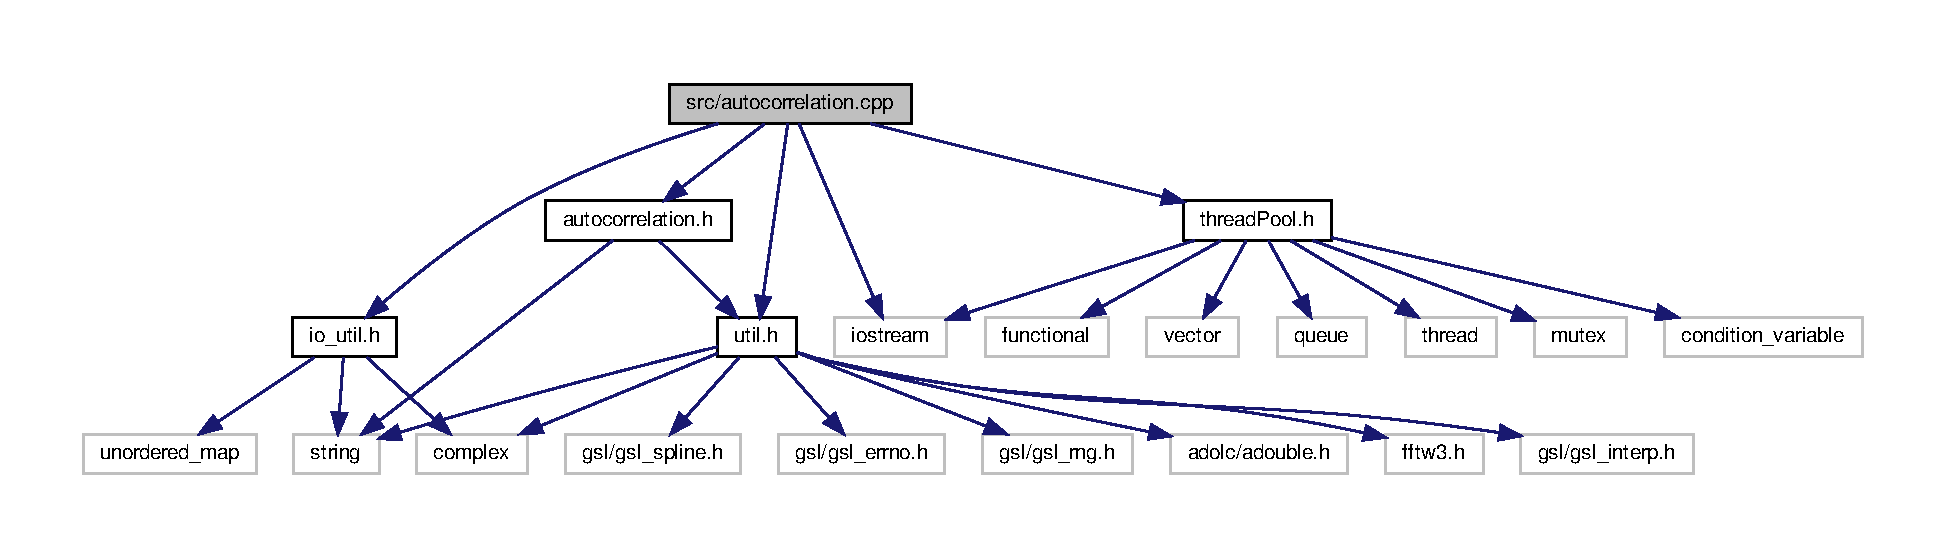
\includegraphics[width=350pt]{autocorrelation_8cpp__incl}
\end{center}
\end{figure}
\doxysubsection*{Macros}
\begin{DoxyCompactItemize}
\item 
\#define \mbox{\hyperlink{autocorrelation_8cpp_a997bd514ed5e4f822888206a11fc8065}{M\+A\+X\+\_\+\+S\+E\+R\+I\+AL}}~20000
\end{DoxyCompactItemize}
\doxysubsection*{Functions}
\begin{DoxyCompactItemize}
\item 
void \mbox{\hyperlink{autocorrelation_8cpp_ad6715011761c1397d215f817654c96b3}{write\+\_\+auto\+\_\+corr\+\_\+file\+\_\+from\+\_\+data\+\_\+file}} (std\+::string autocorr\+\_\+filename, std\+::string datafile, int length, int dimension, int num\+\_\+segments, double target\+\_\+corr, int num\+\_\+threads, bool cumulative)
\item 
void \mbox{\hyperlink{autocorrelation_8cpp_ae925ee63b98024b9832ef2a72c6bca2d}{write\+\_\+auto\+\_\+corr\+\_\+file\+\_\+from\+\_\+data}} (std\+::string autocorr\+\_\+filename, double $\ast$$\ast$data, int length, int dimension, int num\+\_\+segments, double target\+\_\+corr, int num\+\_\+threads, bool cumulative)
\begin{DoxyCompactList}\small\item\em Writes the autocorrelation file from a data array. \end{DoxyCompactList}\item 
void \mbox{\hyperlink{autocorrelation_8cpp_ab9812ba50775fc8453e7b4df14cafca0}{auto\+\_\+corr\+\_\+from\+\_\+data\+\_\+batch}} (double $\ast$$\ast$$\ast$data, int length, int dimension, int chain\+\_\+N, int $\ast$$\ast$$\ast$output, int num\+\_\+segments, double target\+\_\+corr, int num\+\_\+threads, bool cumulative)
\begin{DoxyCompactList}\small\item\em Calculates the autocorrelation length for a set of data for a number of segments for each dimension -- completely host code, utilitizes F\+F\+T\+W3 for longer chuncks of the chains -- Batch version for multiple chains at a time. \end{DoxyCompactList}\item 
void \mbox{\hyperlink{autocorrelation_8cpp_a393fd6777961493a09c5c0923b185d3d}{auto\+\_\+corr\+\_\+from\+\_\+data}} (double $\ast$$\ast$data, int length, int dimension, int $\ast$$\ast$output, int num\+\_\+segments, double target\+\_\+corr, int num\+\_\+threads, bool cumulative)
\begin{DoxyCompactList}\small\item\em Calculates the autocorrelation length for a set of data for a number of segments for each dimension -- completely host code, utilitizes F\+F\+T\+W3 for longer chuncks of the chains. \end{DoxyCompactList}\item 
void \mbox{\hyperlink{autocorrelation_8cpp_a94af5456a8ff9599890ad79deb2101e1}{threaded\+\_\+ac\+\_\+spectral}} (int thread, \mbox{\hyperlink{classthreaded__ac__jobs__fft}{threaded\+\_\+ac\+\_\+jobs\+\_\+fft}} job)
\begin{DoxyCompactList}\small\item\em Internal routine to calculate an spectral autocorrelation job. \end{DoxyCompactList}\item 
void \mbox{\hyperlink{autocorrelation_8cpp_a45c4e43aab21b064274576841fd9f439}{threaded\+\_\+ac\+\_\+serial}} (int thread, \mbox{\hyperlink{classthreaded__ac__jobs__serial}{threaded\+\_\+ac\+\_\+jobs\+\_\+serial}} job)
\begin{DoxyCompactList}\small\item\em Internal routine to calculate a serial autocorrelation job. \end{DoxyCompactList}\item 
double \mbox{\hyperlink{autocorrelation_8cpp_a0e07c16caec7cc0be12258458c96d364}{auto\+\_\+correlation\+\_\+serial}} (double $\ast$arr, int length, int start, double target)
\begin{DoxyCompactList}\small\item\em Calculates the autocorrelation of a chain with the brute force method. \end{DoxyCompactList}\item 
\mbox{\Hypertarget{autocorrelation_8cpp_ab2b46532c9a5857bc08a5b7af33c19d2}\label{autocorrelation_8cpp_ab2b46532c9a5857bc08a5b7af33c19d2}} 
void \mbox{\hyperlink{autocorrelation_8cpp_ab2b46532c9a5857bc08a5b7af33c19d2}{auto\+\_\+correlation\+\_\+spectral}} (double $\ast$chain, int length, double $\ast$autocorr, \mbox{\hyperlink{structfftw__outline}{fftw\+\_\+outline}} $\ast$plan\+\_\+forw, \mbox{\hyperlink{structfftw__outline}{fftw\+\_\+outline}} $\ast$plan\+\_\+rev)
\begin{DoxyCompactList}\small\item\em Wrapper function for convience -- assumes the data array starts at 0. \end{DoxyCompactList}\item 
void \mbox{\hyperlink{autocorrelation_8cpp_a495b7476fb13c79c22c6785ca5c37e9c}{auto\+\_\+correlation\+\_\+spectral}} (double $\ast$chain, int length, int start, double $\ast$autocorr, \mbox{\hyperlink{structfftw__outline}{fftw\+\_\+outline}} $\ast$plan\+\_\+forw, \mbox{\hyperlink{structfftw__outline}{fftw\+\_\+outline}} $\ast$plan\+\_\+rev)
\begin{DoxyCompactList}\small\item\em Faster approximation of the autocorrelation of a chain. Implements F\+F\+T/\+I\+F\+FT -- accepts F\+F\+TW plan as argument for plan reuse and multi-\/threaded applications. \end{DoxyCompactList}\item 
void \mbox{\hyperlink{autocorrelation_8cpp_af5ffdd85c751c9128af46d0459bb4687}{auto\+\_\+correlation\+\_\+spectral}} (double $\ast$chain, int length, double $\ast$autocorr)
\begin{DoxyCompactList}\small\item\em Faster approximation of the autocorrelation of a chain. Implements F\+F\+T/\+I\+F\+FT. \end{DoxyCompactList}\item 
\mbox{\Hypertarget{autocorrelation_8cpp_ab1cc0e008417e22feb67c596f9d84391}\label{autocorrelation_8cpp_ab1cc0e008417e22feb67c596f9d84391}} 
double \mbox{\hyperlink{autocorrelation_8cpp_ab1cc0e008417e22feb67c596f9d84391}{auto\+\_\+correlation}} (double $\ast$arr, int length, double tolerance)
\begin{DoxyCompactList}\small\item\em O\+U\+T\+D\+A\+T\+ED -- numerically finds autocorrelation length -- not reliable. \end{DoxyCompactList}\item 
\mbox{\Hypertarget{autocorrelation_8cpp_ad21465a6ab600a7776dd763e2f8dd577}\label{autocorrelation_8cpp_ad21465a6ab600a7776dd763e2f8dd577}} 
double \mbox{\hyperlink{autocorrelation_8cpp_ad21465a6ab600a7776dd763e2f8dd577}{auto\+\_\+correlation\+\_\+serial\+\_\+old}} (double $\ast$arr, int length)
\begin{DoxyCompactList}\small\item\em O\+U\+T\+D\+A\+T\+ED Calculates the autocorrelation -- less general version. \end{DoxyCompactList}\item 
double \mbox{\hyperlink{autocorrelation_8cpp_a70938f64f11cb3ede5017ebfc6f8f3bd}{auto\+\_\+correlation\+\_\+grid\+\_\+search}} (double $\ast$arr, int length, int box\+\_\+num, int final\+\_\+length, double target\+\_\+length)
\begin{DoxyCompactList}\small\item\em O\+U\+T\+D\+A\+T\+ED -- Grid search method of computing the autocorrelation -- unreliable. \end{DoxyCompactList}\item 
double \mbox{\hyperlink{autocorrelation_8cpp_aee6b6cec0369e5a89823512fde296792}{auto\+\_\+correlation\+\_\+internal}} (double $\ast$arr, int length, int lag, double ave)
\begin{DoxyCompactList}\small\item\em Internal function to compute the auto correlation for a given lag. \end{DoxyCompactList}\item 
void \mbox{\hyperlink{autocorrelation_8cpp_a59cc7470885bbc68e5c9a7725fb237d9}{auto\+\_\+corr\+\_\+intervals\+\_\+outdated}} (double $\ast$data, int length, double $\ast$output, int num\+\_\+segments, double accuracy)
\begin{DoxyCompactList}\small\item\em Function that computes the autocorrelation length on an array of data at set intervals to help determine convergence. \end{DoxyCompactList}\item 
\mbox{\Hypertarget{autocorrelation_8cpp_a8abac9254fd541e086a0fd45ac2a7b11}\label{autocorrelation_8cpp_a8abac9254fd541e086a0fd45ac2a7b11}} 
void \mbox{\hyperlink{autocorrelation_8cpp_a8abac9254fd541e086a0fd45ac2a7b11}{write\+\_\+auto\+\_\+corr\+\_\+file\+\_\+from\+\_\+data}} (std\+::string auto\+\_\+corr\+\_\+filename, double $\ast$$\ast$output, int intervals, int dimension, int N\+\_\+steps)
\begin{DoxyCompactList}\small\item\em O\+U\+T\+D\+A\+T\+ED -- writes autocorrelation lengths for a data array, but only with the serial method and only for a target correlation of .01. \end{DoxyCompactList}\item 
\mbox{\Hypertarget{autocorrelation_8cpp_a96dd06128ac57370dd1acadefb780910}\label{autocorrelation_8cpp_a96dd06128ac57370dd1acadefb780910}} 
void \mbox{\hyperlink{autocorrelation_8cpp_a96dd06128ac57370dd1acadefb780910}{write\+\_\+auto\+\_\+corr\+\_\+file\+\_\+from\+\_\+data\+\_\+file}} (std\+::string auto\+\_\+corr\+\_\+filename, std\+::string output\+\_\+file, int intervals, int dimension, int N\+\_\+steps)
\begin{DoxyCompactList}\small\item\em O\+U\+T\+D\+A\+T\+ED -- writes autocorrelation lengths for a data file, but only with the serial method and only for a target correlation of .01. \end{DoxyCompactList}\end{DoxyCompactItemize}


\doxysubsection{Detailed Description}
Turns out calculating the autocorrelation is more complicated if you want to do it fast, so it gets its own file now

First row is the starting index of that segment

Second row is the length of that segment

If cumulative, the ac is calculated in the following format\+:

$\vert$-\/-\/-\/-\/---$\vert$

$\vert$-\/-\/-\/-\/-\/-\/-\/-\/-\/-\/-\/---$\vert$

$\vert$-\/-\/-\/-\/-\/-\/-\/-\/-\/-\/-\/-\/-\/-\/-\/-\/-\/-\/-\/-\/-\/-\/---$\vert$

...

Else, the ac is calculated as \+:

$\vert$-\/-\/-\/-\/---$\vert$ \begin{DoxyVerb}    |------|

            |--------|
\end{DoxyVerb}


... 

\doxysubsection{Macro Definition Documentation}
\mbox{\Hypertarget{autocorrelation_8cpp_a997bd514ed5e4f822888206a11fc8065}\label{autocorrelation_8cpp_a997bd514ed5e4f822888206a11fc8065}} 
\index{autocorrelation.cpp@{autocorrelation.cpp}!MAX\_SERIAL@{MAX\_SERIAL}}
\index{MAX\_SERIAL@{MAX\_SERIAL}!autocorrelation.cpp@{autocorrelation.cpp}}
\doxysubsubsection{\texorpdfstring{MAX\_SERIAL}{MAX\_SERIAL}}
{\footnotesize\ttfamily \#define M\+A\+X\+\_\+\+S\+E\+R\+I\+AL~20000}

Max length of array to use serial calculation 

\doxysubsection{Function Documentation}
\mbox{\Hypertarget{autocorrelation_8cpp_a393fd6777961493a09c5c0923b185d3d}\label{autocorrelation_8cpp_a393fd6777961493a09c5c0923b185d3d}} 
\index{autocorrelation.cpp@{autocorrelation.cpp}!auto\_corr\_from\_data@{auto\_corr\_from\_data}}
\index{auto\_corr\_from\_data@{auto\_corr\_from\_data}!autocorrelation.cpp@{autocorrelation.cpp}}
\doxysubsubsection{\texorpdfstring{auto\_corr\_from\_data()}{auto\_corr\_from\_data()}}
{\footnotesize\ttfamily void auto\+\_\+corr\+\_\+from\+\_\+data (\begin{DoxyParamCaption}\item[{double $\ast$$\ast$}]{data,  }\item[{int}]{length,  }\item[{int}]{dimension,  }\item[{int $\ast$$\ast$}]{output,  }\item[{int}]{num\+\_\+segments,  }\item[{double}]{target\+\_\+corr,  }\item[{int}]{num\+\_\+threads,  }\item[{bool}]{cumulative }\end{DoxyParamCaption})}



Calculates the autocorrelation length for a set of data for a number of segments for each dimension -- completely host code, utilitizes F\+F\+T\+W3 for longer chuncks of the chains. 

Takes in the data from a sampler, shape data\mbox{[}N\+\_\+steps\mbox{]}\mbox{[}dimension\mbox{]}

Outputs lags that correspond to the target\+\_\+corr -- shape output\mbox{[}dimension\mbox{]}\mbox{[}num\+\_\+segments\mbox{]}

If cumulative, the ac is calculated in the following format\+:

$\vert$-\/-\/-\/-\/---$\vert$

$\vert$-\/-\/-\/-\/-\/-\/-\/-\/-\/-\/-\/---$\vert$

$\vert$-\/-\/-\/-\/-\/-\/-\/-\/-\/-\/-\/-\/-\/-\/-\/-\/-\/-\/-\/-\/-\/-\/---$\vert$

...

Else, the ac is calculated as \+:

$\vert$-\/-\/-\/-\/---$\vert$ \begin{DoxyVerb}    |------|

            |--------|
\end{DoxyVerb}


... 
\begin{DoxyParams}[1]{Parameters}
 & {\em data} & Input data \\
\hline
 & {\em length} & length of input data \\
\hline
 & {\em dimension} & dimension of data \\
\hline
\mbox{\texttt{ out}}  & {\em output} & array that stores the auto-\/corr lengths -\/-\/ array\mbox{[}num\+\_\+segments\mbox{]} \\
\hline
 & {\em num\+\_\+segments} & number of segements to compute the auto-\/corr length \\
\hline
 & {\em target\+\_\+corr} & Autocorrelation for which the autocorrelation length is defined (lag of autocorrelation for which it equals the target\+\_\+corr) \\
\hline
 & {\em num\+\_\+threads} & Total number of threads to use \\
\hline
 & {\em cumulative} & Boolean to calculate the autocorrelation cumulatively \\
\hline
\end{DoxyParams}
\mbox{\Hypertarget{autocorrelation_8cpp_ab9812ba50775fc8453e7b4df14cafca0}\label{autocorrelation_8cpp_ab9812ba50775fc8453e7b4df14cafca0}} 
\index{autocorrelation.cpp@{autocorrelation.cpp}!auto\_corr\_from\_data\_batch@{auto\_corr\_from\_data\_batch}}
\index{auto\_corr\_from\_data\_batch@{auto\_corr\_from\_data\_batch}!autocorrelation.cpp@{autocorrelation.cpp}}
\doxysubsubsection{\texorpdfstring{auto\_corr\_from\_data\_batch()}{auto\_corr\_from\_data\_batch()}}
{\footnotesize\ttfamily void auto\+\_\+corr\+\_\+from\+\_\+data\+\_\+batch (\begin{DoxyParamCaption}\item[{double $\ast$$\ast$$\ast$}]{data,  }\item[{int}]{length,  }\item[{int}]{dimension,  }\item[{int}]{chain\+\_\+N,  }\item[{int $\ast$$\ast$$\ast$}]{output,  }\item[{int}]{num\+\_\+segments,  }\item[{double}]{target\+\_\+corr,  }\item[{int}]{num\+\_\+threads,  }\item[{bool}]{cumulative }\end{DoxyParamCaption})}



Calculates the autocorrelation length for a set of data for a number of segments for each dimension -- completely host code, utilitizes F\+F\+T\+W3 for longer chuncks of the chains -- Batch version for multiple chains at a time. 

Takes in the data from a sampler, shape data\mbox{[}chain\+\_\+N\mbox{]}\mbox{[}N\+\_\+steps\mbox{]}\mbox{[}dimension\mbox{]}

Outputs lags that correspond to the target\+\_\+corr -- shape output\mbox{[}chain\+\_\+N\mbox{]}\mbox{[}dimension\mbox{]}\mbox{[}num\+\_\+segments\mbox{]}

If cumulative, the ac is calculated in the following format\+:

$\vert$-\/-\/-\/-\/---$\vert$

$\vert$-\/-\/-\/-\/-\/-\/-\/-\/-\/-\/-\/---$\vert$

$\vert$-\/-\/-\/-\/-\/-\/-\/-\/-\/-\/-\/-\/-\/-\/-\/-\/-\/-\/-\/-\/-\/-\/---$\vert$

...

Else, the ac is calculated as \+:

$\vert$-\/-\/-\/-\/---$\vert$ \begin{DoxyVerb}    |------|

            |--------|
\end{DoxyVerb}


... 
\begin{DoxyParams}[1]{Parameters}
 & {\em data} & Input data \\
\hline
 & {\em length} & length of input data \\
\hline
 & {\em dimension} & dimension of data \\
\hline
\mbox{\texttt{ out}}  & {\em output} & array that stores the auto-\/corr lengths -\/-\/ array\mbox{[}num\+\_\+segments\mbox{]} \\
\hline
 & {\em num\+\_\+segments} & number of segements to compute the auto-\/corr length \\
\hline
 & {\em target\+\_\+corr} & Autocorrelation for which the autocorrelation length is defined (lag of autocorrelation for which it equals the target\+\_\+corr) \\
\hline
 & {\em num\+\_\+threads} & Total number of threads to use \\
\hline
 & {\em cumulative} & Boolean to calculate the autocorrelation cumulatively \\
\hline
\end{DoxyParams}
\mbox{\Hypertarget{autocorrelation_8cpp_a59cc7470885bbc68e5c9a7725fb237d9}\label{autocorrelation_8cpp_a59cc7470885bbc68e5c9a7725fb237d9}} 
\index{autocorrelation.cpp@{autocorrelation.cpp}!auto\_corr\_intervals\_outdated@{auto\_corr\_intervals\_outdated}}
\index{auto\_corr\_intervals\_outdated@{auto\_corr\_intervals\_outdated}!autocorrelation.cpp@{autocorrelation.cpp}}
\doxysubsubsection{\texorpdfstring{auto\_corr\_intervals\_outdated()}{auto\_corr\_intervals\_outdated()}}
{\footnotesize\ttfamily void auto\+\_\+corr\+\_\+intervals\+\_\+outdated (\begin{DoxyParamCaption}\item[{double $\ast$}]{data,  }\item[{int}]{length,  }\item[{double $\ast$}]{output,  }\item[{int}]{num\+\_\+segments,  }\item[{double}]{accuracy }\end{DoxyParamCaption})}



Function that computes the autocorrelation length on an array of data at set intervals to help determine convergence. 

outdated version -- new version uses F\+F\+Ts 
\begin{DoxyParams}[1]{Parameters}
 & {\em data} & Input data \\
\hline
 & {\em length} & length of input data \\
\hline
\mbox{\texttt{ out}}  & {\em output} & array that stores the auto-\/corr lengths -\/-\/ array\mbox{[}num\+\_\+segments\mbox{]} \\
\hline
 & {\em num\+\_\+segments} & number of segements to compute the auto-\/corr length \\
\hline
 & {\em accuracy} & longer chains are computed numerically, this specifies the tolerance \\
\hline
\end{DoxyParams}
\mbox{\Hypertarget{autocorrelation_8cpp_a70938f64f11cb3ede5017ebfc6f8f3bd}\label{autocorrelation_8cpp_a70938f64f11cb3ede5017ebfc6f8f3bd}} 
\index{autocorrelation.cpp@{autocorrelation.cpp}!auto\_correlation\_grid\_search@{auto\_correlation\_grid\_search}}
\index{auto\_correlation\_grid\_search@{auto\_correlation\_grid\_search}!autocorrelation.cpp@{autocorrelation.cpp}}
\doxysubsubsection{\texorpdfstring{auto\_correlation\_grid\_search()}{auto\_correlation\_grid\_search()}}
{\footnotesize\ttfamily double auto\+\_\+correlation\+\_\+grid\+\_\+search (\begin{DoxyParamCaption}\item[{double $\ast$}]{arr,  }\item[{int}]{length,  }\item[{int}]{box\+\_\+num,  }\item[{int}]{final\+\_\+length,  }\item[{double}]{target\+\_\+length }\end{DoxyParamCaption})}



O\+U\+T\+D\+A\+T\+ED -- Grid search method of computing the autocorrelation -- unreliable. 

Hopefully more reliable than the box-\/search method, which can sometimes get caught in a recursive loop when the stepsize isn\textquotesingle{}t tuned, but also faster than the basic linear, serial search 
\begin{DoxyParams}{Parameters}
{\em arr} & Input array to use for autocorrelation \\
\hline
{\em length} & Length of input array \\
\hline
{\em box\+\_\+num} & number of boxes to use for each iteration, default is 10 \\
\hline
{\em final\+\_\+length} & number of elements per box at which the grid search ends and the serial calculation begins \\
\hline
{\em target\+\_\+length} & target correlation that corresponds to the returned lag \\
\hline
\end{DoxyParams}
\mbox{\Hypertarget{autocorrelation_8cpp_aee6b6cec0369e5a89823512fde296792}\label{autocorrelation_8cpp_aee6b6cec0369e5a89823512fde296792}} 
\index{autocorrelation.cpp@{autocorrelation.cpp}!auto\_correlation\_internal@{auto\_correlation\_internal}}
\index{auto\_correlation\_internal@{auto\_correlation\_internal}!autocorrelation.cpp@{autocorrelation.cpp}}
\doxysubsubsection{\texorpdfstring{auto\_correlation\_internal()}{auto\_correlation\_internal()}}
{\footnotesize\ttfamily double auto\+\_\+correlation\+\_\+internal (\begin{DoxyParamCaption}\item[{double $\ast$}]{arr,  }\item[{int}]{length,  }\item[{int}]{lag,  }\item[{double}]{ave }\end{DoxyParamCaption})}



Internal function to compute the auto correlation for a given lag. 

\mbox{\Hypertarget{autocorrelation_8cpp_a0e07c16caec7cc0be12258458c96d364}\label{autocorrelation_8cpp_a0e07c16caec7cc0be12258458c96d364}} 
\index{autocorrelation.cpp@{autocorrelation.cpp}!auto\_correlation\_serial@{auto\_correlation\_serial}}
\index{auto\_correlation\_serial@{auto\_correlation\_serial}!autocorrelation.cpp@{autocorrelation.cpp}}
\doxysubsubsection{\texorpdfstring{auto\_correlation\_serial()}{auto\_correlation\_serial()}}
{\footnotesize\ttfamily double auto\+\_\+correlation\+\_\+serial (\begin{DoxyParamCaption}\item[{double $\ast$}]{arr,  }\item[{int}]{length,  }\item[{int}]{start,  }\item[{double}]{target }\end{DoxyParamCaption})}



Calculates the autocorrelation of a chain with the brute force method. 


\begin{DoxyParams}{Parameters}
{\em arr} & input array \\
\hline
{\em length} & Length of input array \\
\hline
{\em start} & starting index (probably 0) \\
\hline
{\em target} & Target autocorrelation for which \`{}\`{}length\textquotesingle{}\textquotesingle{} is defined \\
\hline
\end{DoxyParams}
\mbox{\Hypertarget{autocorrelation_8cpp_af5ffdd85c751c9128af46d0459bb4687}\label{autocorrelation_8cpp_af5ffdd85c751c9128af46d0459bb4687}} 
\index{autocorrelation.cpp@{autocorrelation.cpp}!auto\_correlation\_spectral@{auto\_correlation\_spectral}}
\index{auto\_correlation\_spectral@{auto\_correlation\_spectral}!autocorrelation.cpp@{autocorrelation.cpp}}
\doxysubsubsection{\texorpdfstring{auto\_correlation\_spectral()}{auto\_correlation\_spectral()}\hspace{0.1cm}{\footnotesize\ttfamily [1/2]}}
{\footnotesize\ttfamily void auto\+\_\+correlation\+\_\+spectral (\begin{DoxyParamCaption}\item[{double $\ast$}]{chain,  }\item[{int}]{length,  }\item[{double $\ast$}]{autocorr }\end{DoxyParamCaption})}



Faster approximation of the autocorrelation of a chain. Implements F\+F\+T/\+I\+F\+FT. 

Based on the Wiener-\/\+Khinchin Theorem.

Algorithm used from \href{https://lingpipe-blog.com/2012/06/08/autocorrelation-fft-kiss-eigen/}{\texttt{ https\+://lingpipe-\/blog.\+com/2012/06/08/autocorrelation-\/fft-\/kiss-\/eigen/}} \mbox{\Hypertarget{autocorrelation_8cpp_a495b7476fb13c79c22c6785ca5c37e9c}\label{autocorrelation_8cpp_a495b7476fb13c79c22c6785ca5c37e9c}} 
\index{autocorrelation.cpp@{autocorrelation.cpp}!auto\_correlation\_spectral@{auto\_correlation\_spectral}}
\index{auto\_correlation\_spectral@{auto\_correlation\_spectral}!autocorrelation.cpp@{autocorrelation.cpp}}
\doxysubsubsection{\texorpdfstring{auto\_correlation\_spectral()}{auto\_correlation\_spectral()}\hspace{0.1cm}{\footnotesize\ttfamily [2/2]}}
{\footnotesize\ttfamily void auto\+\_\+correlation\+\_\+spectral (\begin{DoxyParamCaption}\item[{double $\ast$}]{chain,  }\item[{int}]{length,  }\item[{int}]{start,  }\item[{double $\ast$}]{autocorr,  }\item[{\mbox{\hyperlink{structfftw__outline}{fftw\+\_\+outline}} $\ast$}]{plan\+\_\+forw,  }\item[{\mbox{\hyperlink{structfftw__outline}{fftw\+\_\+outline}} $\ast$}]{plan\+\_\+rev }\end{DoxyParamCaption})}



Faster approximation of the autocorrelation of a chain. Implements F\+F\+T/\+I\+F\+FT -- accepts F\+F\+TW plan as argument for plan reuse and multi-\/threaded applications. 

Based on the Wiener-\/\+Khinchin Theorem.

Algorithm used from \href{https://lingpipe-blog.com/2012/06/08/autocorrelation-fft-kiss-eigen/}{\texttt{ https\+://lingpipe-\/blog.\+com/2012/06/08/autocorrelation-\/fft-\/kiss-\/eigen/}}

{\itshape N\+O\+TE} the length used in initializing the fftw plans should be L = pow(2, std\+::ceil( std\+::log2(length) ) ) -- the plans are padded so the total length is a power of two

Option to provide starting index for multi-\/dimension arrays in collapsed to one dimension

length is the length of the segment to be analyzed, not necessarily the dimension of the chain \mbox{\Hypertarget{autocorrelation_8cpp_a45c4e43aab21b064274576841fd9f439}\label{autocorrelation_8cpp_a45c4e43aab21b064274576841fd9f439}} 
\index{autocorrelation.cpp@{autocorrelation.cpp}!threaded\_ac\_serial@{threaded\_ac\_serial}}
\index{threaded\_ac\_serial@{threaded\_ac\_serial}!autocorrelation.cpp@{autocorrelation.cpp}}
\doxysubsubsection{\texorpdfstring{threaded\_ac\_serial()}{threaded\_ac\_serial()}}
{\footnotesize\ttfamily void threaded\+\_\+ac\+\_\+serial (\begin{DoxyParamCaption}\item[{int}]{thread,  }\item[{\mbox{\hyperlink{classthreaded__ac__jobs__serial}{threaded\+\_\+ac\+\_\+jobs\+\_\+serial}}}]{job }\end{DoxyParamCaption})}



Internal routine to calculate a serial autocorrelation job. 

Allows for a more efficient use of the \mbox{\hyperlink{classthreadPool}{thread\+Pool}} class \mbox{\Hypertarget{autocorrelation_8cpp_a94af5456a8ff9599890ad79deb2101e1}\label{autocorrelation_8cpp_a94af5456a8ff9599890ad79deb2101e1}} 
\index{autocorrelation.cpp@{autocorrelation.cpp}!threaded\_ac\_spectral@{threaded\_ac\_spectral}}
\index{threaded\_ac\_spectral@{threaded\_ac\_spectral}!autocorrelation.cpp@{autocorrelation.cpp}}
\doxysubsubsection{\texorpdfstring{threaded\_ac\_spectral()}{threaded\_ac\_spectral()}}
{\footnotesize\ttfamily void threaded\+\_\+ac\+\_\+spectral (\begin{DoxyParamCaption}\item[{int}]{thread,  }\item[{\mbox{\hyperlink{classthreaded__ac__jobs__fft}{threaded\+\_\+ac\+\_\+jobs\+\_\+fft}}}]{job }\end{DoxyParamCaption})}



Internal routine to calculate an spectral autocorrelation job. 

Allows for a more efficient use of the \mbox{\hyperlink{classthreadPool}{thread\+Pool}} class \mbox{\Hypertarget{autocorrelation_8cpp_ae925ee63b98024b9832ef2a72c6bca2d}\label{autocorrelation_8cpp_ae925ee63b98024b9832ef2a72c6bca2d}} 
\index{autocorrelation.cpp@{autocorrelation.cpp}!write\_auto\_corr\_file\_from\_data@{write\_auto\_corr\_file\_from\_data}}
\index{write\_auto\_corr\_file\_from\_data@{write\_auto\_corr\_file\_from\_data}!autocorrelation.cpp@{autocorrelation.cpp}}
\doxysubsubsection{\texorpdfstring{write\_auto\_corr\_file\_from\_data()}{write\_auto\_corr\_file\_from\_data()}}
{\footnotesize\ttfamily void write\+\_\+auto\+\_\+corr\+\_\+file\+\_\+from\+\_\+data (\begin{DoxyParamCaption}\item[{std\+::string}]{autocorr\+\_\+filename,  }\item[{double $\ast$$\ast$}]{data,  }\item[{int}]{length,  }\item[{int}]{dimension,  }\item[{int}]{num\+\_\+segments,  }\item[{double}]{target\+\_\+corr,  }\item[{int}]{num\+\_\+threads,  }\item[{bool}]{cumulative }\end{DoxyParamCaption})}



Writes the autocorrelation file from a data array. 

First row is the starting index of that segment

Second row is the length of that segment

If cumulative, the ac is calculated in the following format\+:

$\vert$-\/-\/-\/-\/---$\vert$

$\vert$-\/-\/-\/-\/-\/-\/-\/-\/-\/-\/-\/---$\vert$

$\vert$-\/-\/-\/-\/-\/-\/-\/-\/-\/-\/-\/-\/-\/-\/-\/-\/-\/-\/-\/-\/-\/-\/---$\vert$

...

Else, the ac is calculated as \+:

$\vert$-\/-\/-\/-\/---$\vert$ \begin{DoxyVerb}    |------|

            |--------|
\end{DoxyVerb}


... 
\begin{DoxyParams}{Parameters}
{\em autocorr\+\_\+filename} & Name of the file to write the autocorrelation to \\
\hline
{\em data} & Input chains \\
\hline
{\em length} & length of input data \\
\hline
{\em dimension} & dimension of data \\
\hline
{\em num\+\_\+segments} & number of segements to compute the auto-\/corr length \\
\hline
{\em target\+\_\+corr} & Autocorrelation for which the autocorrelation length is defined (lag of autocorrelation for which it equals the target\+\_\+corr) \\
\hline
{\em num\+\_\+threads} & Total number of threads to use \\
\hline
{\em cumulative} & Boolean to calculate the autocorrelation cumulatively \\
\hline
\end{DoxyParams}
\mbox{\Hypertarget{autocorrelation_8cpp_ad6715011761c1397d215f817654c96b3}\label{autocorrelation_8cpp_ad6715011761c1397d215f817654c96b3}} 
\index{autocorrelation.cpp@{autocorrelation.cpp}!write\_auto\_corr\_file\_from\_data\_file@{write\_auto\_corr\_file\_from\_data\_file}}
\index{write\_auto\_corr\_file\_from\_data\_file@{write\_auto\_corr\_file\_from\_data\_file}!autocorrelation.cpp@{autocorrelation.cpp}}
\doxysubsubsection{\texorpdfstring{write\_auto\_corr\_file\_from\_data\_file()}{write\_auto\_corr\_file\_from\_data\_file()}}
{\footnotesize\ttfamily void write\+\_\+auto\+\_\+corr\+\_\+file\+\_\+from\+\_\+data\+\_\+file (\begin{DoxyParamCaption}\item[{std\+::string}]{autocorr\+\_\+filename,  }\item[{std\+::string}]{datafile,  }\item[{int}]{length,  }\item[{int}]{dimension,  }\item[{int}]{num\+\_\+segments,  }\item[{double}]{target\+\_\+corr,  }\item[{int}]{num\+\_\+threads,  }\item[{bool}]{cumulative }\end{DoxyParamCaption})}


\begin{DoxyParams}{Parameters}
{\em length} & length of input data \\
\hline
{\em dimension} & dimension of data \\
\hline
{\em num\+\_\+segments} & number of segements to compute the auto-\/corr length \\
\hline
{\em target\+\_\+corr} & Autocorrelation for which the autocorrelation length is defined (lag of autocorrelation for which it equals the target\+\_\+corr) \\
\hline
{\em num\+\_\+threads} & Total number of threads to use \\
\hline
{\em cumulative} & Boolean to calculate the autocorrelation cumulatively \\
\hline
\end{DoxyParams}

\hypertarget{autocorrelation__cuda_8cu}{}\section{src/autocorrelation\+\_\+cuda.cu File Reference}
\label{autocorrelation__cuda_8cu}\index{src/autocorrelation\+\_\+cuda.\+cu@{src/autocorrelation\+\_\+cuda.\+cu}}
{\ttfamily \#include \char`\"{}autocorrelation\+\_\+cuda.\+h\char`\"{}}\newline
{\ttfamily \#include \char`\"{}autocorrelation\+\_\+cuda.\+hu\char`\"{}}\newline
{\ttfamily \#include \char`\"{}util.\+h\char`\"{}}\newline
{\ttfamily \#include \char`\"{}io\+\_\+util.\+h\char`\"{}}\newline
{\ttfamily \#include $<$iostream$>$}\newline
{\ttfamily \#include $<$condition\+\_\+variable$>$}\newline
{\ttfamily \#include $<$thread$>$}\newline
{\ttfamily \#include $<$queue$>$}\newline
{\ttfamily \#include $<$functional$>$}\newline
{\ttfamily \#include $<$mutex$>$}\newline
{\ttfamily \#include $<$unistd.\+h$>$}\newline
{\ttfamily \#include $<$thread\+Pool.\+h$>$}\newline
{\ttfamily \#include $<$cufft.\+h$>$}\newline
Include dependency graph for autocorrelation\+\_\+cuda.\+cu\+:\nopagebreak
\begin{figure}[H]
\begin{center}
\leavevmode
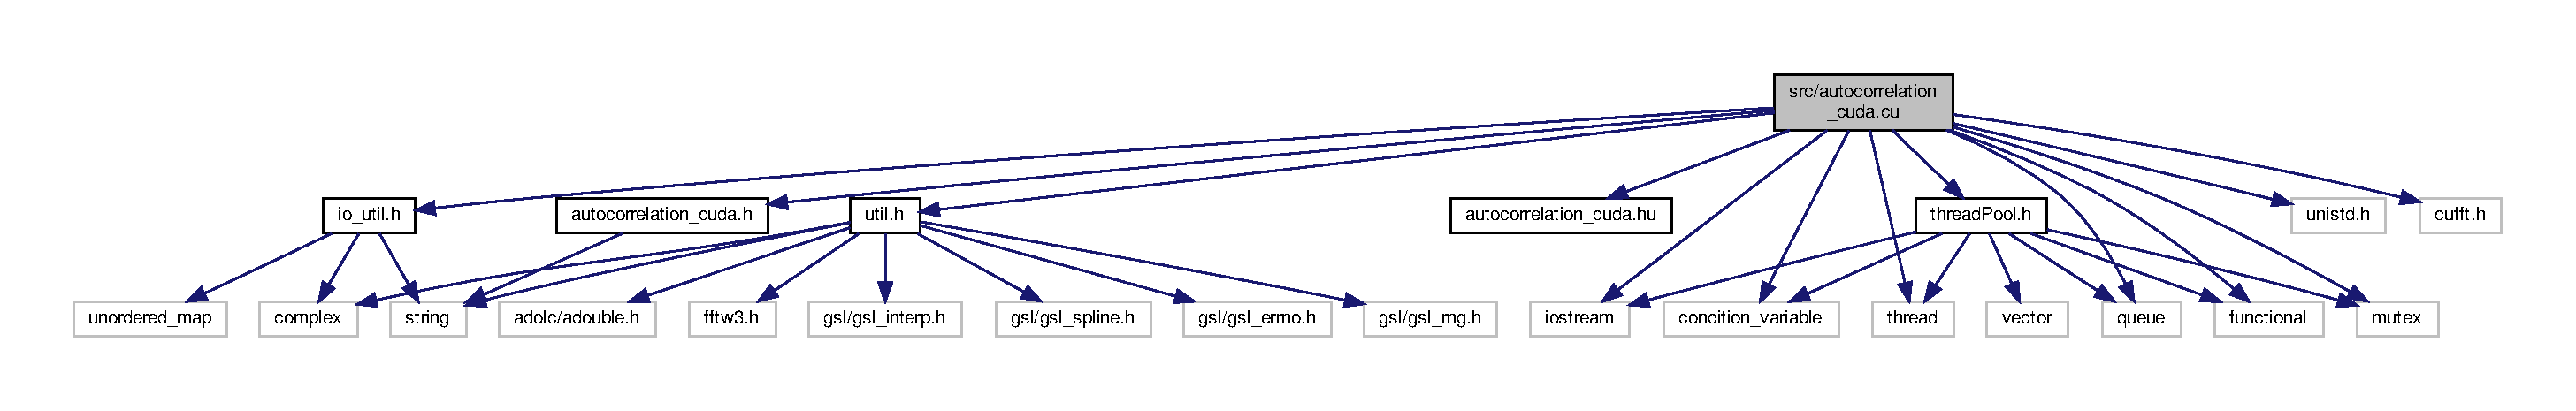
\includegraphics[width=350pt]{autocorrelation__cuda_8cu__incl}
\end{center}
\end{figure}
\subsection*{Functions}
\begin{DoxyCompactItemize}
\item 
\+\_\+\+\_\+device\+\_\+\+\_\+ \+\_\+\+\_\+host\+\_\+\+\_\+ void \hyperlink{autocorrelation__cuda_8cu_a366f884938ea0477409e8d52f0309a44}{auto\+\_\+corr\+\_\+internal} (double $\ast$arr, int length, int lag, double average, double $\ast$corr, int start\+\_\+id)
\begin{DoxyCompactList}\small\item\em Internal function to calculate the autocorrelation for a given lag Customized for the thread pool architecture, with extra arguments because of the way the memory is allocated. \end{DoxyCompactList}\item 
\+\_\+\+\_\+global\+\_\+\+\_\+ void \hyperlink{autocorrelation__cuda_8cu_ad8cff0e627281b397e017fec619b38a5}{auto\+\_\+corr\+\_\+internal\+\_\+kernal} (double $\ast$arr, int length, double average, int $\ast$rho\+\_\+index, double target\+\_\+corr, double var, int start\+\_\+id)
\begin{DoxyCompactList}\small\item\em Internal function to launch the C\+U\+DA kernel for a range of autocorrelations. \end{DoxyCompactList}\item 
void \hyperlink{autocorrelation__cuda_8cu_a4b4ed2b89a95a13abf59d6e373316770}{write\+\_\+file\+\_\+auto\+\_\+corr\+\_\+from\+\_\+data\+\_\+file\+\_\+accel} (std\+::string acfile, std\+::string chains\+\_\+file, int dimension, int N\+\_\+steps, int num\+\_\+segments, double target\+\_\+corr)
\begin{DoxyCompactList}\small\item\em Write data file for autocorrelation lengths of the data given a data file name, as written by the mcmc\+\_\+sampler. \end{DoxyCompactList}\item 
void \hyperlink{autocorrelation__cuda_8cu_a2ba6f84b0a37e4fc578791f745ee9912}{write\+\_\+file\+\_\+auto\+\_\+corr\+\_\+from\+\_\+data\+\_\+accel} (std\+::string acfile, double $\ast$$\ast$chains, int dimension, int N\+\_\+steps, int num\+\_\+segments, double target\+\_\+corr)
\begin{DoxyCompactList}\small\item\em Write data file given output chains, as formatted by the mcmc\+\_\+sampler. \end{DoxyCompactList}\item 
void \hyperlink{autocorrelation__cuda_8cu_a32229785a7faa2b81d4894aafc640ed5}{auto\+\_\+corr\+\_\+from\+\_\+data\+\_\+accel} (double $\ast$$\ast$output, int dimension, int N\+\_\+steps, int num\+\_\+segments, double target\+\_\+corr, double $\ast$$\ast$autocorr)
\begin{DoxyCompactList}\small\item\em Find autocorrelation of data at different points in the chain length and output to autocorr. \end{DoxyCompactList}\item 
void \hyperlink{autocorrelation__cuda_8cu_a51bcc72596ce81494ca39a8aa7a74c53}{ac\+\_\+gpu\+\_\+wrapper} (int thread, int job\+\_\+id)
\begin{DoxyCompactList}\small\item\em Wrapper function for the thread pool. \end{DoxyCompactList}\item 
\mbox{\Hypertarget{autocorrelation__cuda_8cu_a3cf30342474041a00ac261eb5e7afed3}\label{autocorrelation__cuda_8cu_a3cf30342474041a00ac261eb5e7afed3}} 
void \hyperlink{autocorrelation__cuda_8cu_a3cf30342474041a00ac261eb5e7afed3}{launch\+\_\+ac\+\_\+gpu} (int device, int element, double $\ast$$\ast$data, int length, int dimension, double target\+\_\+corr, int num\+\_\+segments)
\begin{DoxyCompactList}\small\item\em Launch the G\+PU kernel, formatted for the thread pool. \end{DoxyCompactList}\item 
void \hyperlink{autocorrelation__cuda_8cu_a0516461a0e02bf12da6c199061247a77}{allocate\+\_\+gpu\+\_\+plan} (\hyperlink{structGPUplan}{G\+P\+Uplan} $\ast$plan, int data\+\_\+length, int dimension, int num\+\_\+segments)
\begin{DoxyCompactList}\small\item\em Allocates memory for autocorrelation--G\+PU structure. \end{DoxyCompactList}\item 
void \hyperlink{autocorrelation__cuda_8cu_a131867ca45185be0af927a5ec7d7645d}{deallocate\+\_\+gpu\+\_\+plan} (\hyperlink{structGPUplan}{G\+P\+Uplan} $\ast$plan, int data\+\_\+length, int dimension, int num\+\_\+segments)
\begin{DoxyCompactList}\small\item\em Deallocates memory for the autocorrelation--G\+PU structure. \end{DoxyCompactList}\item 
void \hyperlink{autocorrelation__cuda_8cu_a00159a0e9eb7e40725a034becb3110c0}{copy\+\_\+data\+\_\+to\+\_\+device} (\hyperlink{structGPUplan}{G\+P\+Uplan} $\ast$plan, double $\ast$$\ast$input\+\_\+data, int data\+\_\+length, int dimension, int num\+\_\+segments)
\begin{DoxyCompactList}\small\item\em Copy data to device before starting kernels. \end{DoxyCompactList}\end{DoxyCompactItemize}
\subsection*{Variables}
\begin{DoxyCompactItemize}
\item 
\mbox{\Hypertarget{autocorrelation__cuda_8cu_a64b38211e5791c7f4eef2bfaf85e1149}\label{autocorrelation__cuda_8cu_a64b38211e5791c7f4eef2bfaf85e1149}} 
\hyperlink{structGPUplan}{G\+P\+Uplan} $\ast$ {\bfseries plans\+\_\+global}
\end{DoxyCompactItemize}


\subsection{Function Documentation}
\mbox{\Hypertarget{autocorrelation__cuda_8cu_a51bcc72596ce81494ca39a8aa7a74c53}\label{autocorrelation__cuda_8cu_a51bcc72596ce81494ca39a8aa7a74c53}} 
\index{autocorrelation\+\_\+cuda.\+cu@{autocorrelation\+\_\+cuda.\+cu}!ac\+\_\+gpu\+\_\+wrapper@{ac\+\_\+gpu\+\_\+wrapper}}
\index{ac\+\_\+gpu\+\_\+wrapper@{ac\+\_\+gpu\+\_\+wrapper}!autocorrelation\+\_\+cuda.\+cu@{autocorrelation\+\_\+cuda.\+cu}}
\subsubsection{\texorpdfstring{ac\+\_\+gpu\+\_\+wrapper()}{ac\_gpu\_wrapper()}}
{\footnotesize\ttfamily void ac\+\_\+gpu\+\_\+wrapper (\begin{DoxyParamCaption}\item[{int}]{thread,  }\item[{int}]{job\+\_\+id }\end{DoxyParamCaption})}



Wrapper function for the thread pool. 


\begin{DoxyParams}{Parameters}
{\em thread} & Host thread \\
\hline
{\em job\+\_\+id} & Job ID \\
\hline
\end{DoxyParams}
\mbox{\Hypertarget{autocorrelation__cuda_8cu_a0516461a0e02bf12da6c199061247a77}\label{autocorrelation__cuda_8cu_a0516461a0e02bf12da6c199061247a77}} 
\index{autocorrelation\+\_\+cuda.\+cu@{autocorrelation\+\_\+cuda.\+cu}!allocate\+\_\+gpu\+\_\+plan@{allocate\+\_\+gpu\+\_\+plan}}
\index{allocate\+\_\+gpu\+\_\+plan@{allocate\+\_\+gpu\+\_\+plan}!autocorrelation\+\_\+cuda.\+cu@{autocorrelation\+\_\+cuda.\+cu}}
\subsubsection{\texorpdfstring{allocate\+\_\+gpu\+\_\+plan()}{allocate\_gpu\_plan()}}
{\footnotesize\ttfamily void allocate\+\_\+gpu\+\_\+plan (\begin{DoxyParamCaption}\item[{\hyperlink{structGPUplan}{G\+P\+Uplan} $\ast$}]{plan,  }\item[{int}]{data\+\_\+length,  }\item[{int}]{dimension,  }\item[{int}]{num\+\_\+segments }\end{DoxyParamCaption})}



Allocates memory for autocorrelation--G\+PU structure. 


\begin{DoxyParams}{Parameters}
{\em plan} & Structure for G\+PU plan \\
\hline
{\em data\+\_\+length} & Length of data \\
\hline
{\em dimension} & Dimension of the data \\
\hline
{\em num\+\_\+segments} & Number of segments to calculate the autocorrelation length \\
\hline
\end{DoxyParams}
\mbox{\Hypertarget{autocorrelation__cuda_8cu_a32229785a7faa2b81d4894aafc640ed5}\label{autocorrelation__cuda_8cu_a32229785a7faa2b81d4894aafc640ed5}} 
\index{autocorrelation\+\_\+cuda.\+cu@{autocorrelation\+\_\+cuda.\+cu}!auto\+\_\+corr\+\_\+from\+\_\+data\+\_\+accel@{auto\+\_\+corr\+\_\+from\+\_\+data\+\_\+accel}}
\index{auto\+\_\+corr\+\_\+from\+\_\+data\+\_\+accel@{auto\+\_\+corr\+\_\+from\+\_\+data\+\_\+accel}!autocorrelation\+\_\+cuda.\+cu@{autocorrelation\+\_\+cuda.\+cu}}
\subsubsection{\texorpdfstring{auto\+\_\+corr\+\_\+from\+\_\+data\+\_\+accel()}{auto\_corr\_from\_data\_accel()}}
{\footnotesize\ttfamily void auto\+\_\+corr\+\_\+from\+\_\+data\+\_\+accel (\begin{DoxyParamCaption}\item[{double $\ast$$\ast$}]{output,  }\item[{int}]{dimension,  }\item[{int}]{N\+\_\+steps,  }\item[{int}]{num\+\_\+segments,  }\item[{double}]{target\+\_\+corr,  }\item[{double $\ast$$\ast$}]{autocorr }\end{DoxyParamCaption})}



Find autocorrelation of data at different points in the chain length and output to autocorr. 


\begin{DoxyParams}[1]{Parameters}
 & {\em output} & Chain data input \\
\hline
 & {\em dimension} & Dimension of the data \\
\hline
 & {\em N\+\_\+steps} & Number of steps in the data \\
\hline
 & {\em num\+\_\+segments} & number of segments to calculate the autocorrelation length \\
\hline
 & {\em target\+\_\+corr} & Target correlation ratio \\
\hline
\mbox{\tt out}  & {\em autocorr} & Autocorrelation lengths for the different segments \\
\hline
\end{DoxyParams}
\mbox{\Hypertarget{autocorrelation__cuda_8cu_a366f884938ea0477409e8d52f0309a44}\label{autocorrelation__cuda_8cu_a366f884938ea0477409e8d52f0309a44}} 
\index{autocorrelation\+\_\+cuda.\+cu@{autocorrelation\+\_\+cuda.\+cu}!auto\+\_\+corr\+\_\+internal@{auto\+\_\+corr\+\_\+internal}}
\index{auto\+\_\+corr\+\_\+internal@{auto\+\_\+corr\+\_\+internal}!autocorrelation\+\_\+cuda.\+cu@{autocorrelation\+\_\+cuda.\+cu}}
\subsubsection{\texorpdfstring{auto\+\_\+corr\+\_\+internal()}{auto\_corr\_internal()}}
{\footnotesize\ttfamily \+\_\+\+\_\+device\+\_\+\+\_\+ \+\_\+\+\_\+host\+\_\+\+\_\+ void auto\+\_\+corr\+\_\+internal (\begin{DoxyParamCaption}\item[{double $\ast$}]{arr,  }\item[{int}]{length,  }\item[{int}]{lag,  }\item[{double}]{average,  }\item[{double $\ast$}]{corr,  }\item[{int}]{start\+\_\+id }\end{DoxyParamCaption})}



Internal function to calculate the autocorrelation for a given lag Customized for the thread pool architecture, with extra arguments because of the way the memory is allocated. 


\begin{DoxyParams}[1]{Parameters}
 & {\em arr} & Input array of data \\
\hline
 & {\em length} & Length of input array \\
\hline
 & {\em lag} & Lag to be used to calculate the correlation \\
\hline
 & {\em average} & Average of the array arr \\
\hline
\mbox{\tt out}  & {\em corr} & output correlation \\
\hline
 & {\em start\+\_\+id} & ID of location to start calculation -- input arrary arr is assumed to be contiguous for multiple dimensions \\
\hline
\end{DoxyParams}
\mbox{\Hypertarget{autocorrelation__cuda_8cu_ad8cff0e627281b397e017fec619b38a5}\label{autocorrelation__cuda_8cu_ad8cff0e627281b397e017fec619b38a5}} 
\index{autocorrelation\+\_\+cuda.\+cu@{autocorrelation\+\_\+cuda.\+cu}!auto\+\_\+corr\+\_\+internal\+\_\+kernal@{auto\+\_\+corr\+\_\+internal\+\_\+kernal}}
\index{auto\+\_\+corr\+\_\+internal\+\_\+kernal@{auto\+\_\+corr\+\_\+internal\+\_\+kernal}!autocorrelation\+\_\+cuda.\+cu@{autocorrelation\+\_\+cuda.\+cu}}
\subsubsection{\texorpdfstring{auto\+\_\+corr\+\_\+internal\+\_\+kernal()}{auto\_corr\_internal\_kernal()}}
{\footnotesize\ttfamily \+\_\+\+\_\+global\+\_\+\+\_\+ void auto\+\_\+corr\+\_\+internal\+\_\+kernal (\begin{DoxyParamCaption}\item[{double $\ast$}]{arr,  }\item[{int}]{length,  }\item[{double}]{average,  }\item[{int $\ast$}]{rho\+\_\+index,  }\item[{double}]{target\+\_\+corr,  }\item[{double}]{var,  }\item[{int}]{start\+\_\+id }\end{DoxyParamCaption})}



Internal function to launch the C\+U\+DA kernel for a range of autocorrelations. 

Correlation function used\+:

rho(lag) = 1 / (length -\/ lag)  (arr\mbox{[}i+lag\mbox{]}-\/average) ( arr\mbox{[}i\mbox{]}-\/ average)

target\+\_\+corr = rho(rho\+\_\+index)/rho(0) = rho(rho\+\_\+index)/var 
\begin{DoxyParams}[1]{Parameters}
 & {\em arr} & Input array of data \\
\hline
 & {\em length} & Length of data array \\
\hline
 & {\em average} & Average of input data \\
\hline
\mbox{\tt out}  & {\em rho\+\_\+index} & Index of the lag that results ina correlation ratio target\+\_\+corr \\
\hline
 & {\em target\+\_\+corr} & Target correlation ratio rho(lag)/rho(0) = target\+\_\+corr \\
\hline
 & {\em var} & Variance rho(0) \\
\hline
 & {\em start\+\_\+id} & Starting index to use for the data array arr \\
\hline
\end{DoxyParams}
\mbox{\Hypertarget{autocorrelation__cuda_8cu_a00159a0e9eb7e40725a034becb3110c0}\label{autocorrelation__cuda_8cu_a00159a0e9eb7e40725a034becb3110c0}} 
\index{autocorrelation\+\_\+cuda.\+cu@{autocorrelation\+\_\+cuda.\+cu}!copy\+\_\+data\+\_\+to\+\_\+device@{copy\+\_\+data\+\_\+to\+\_\+device}}
\index{copy\+\_\+data\+\_\+to\+\_\+device@{copy\+\_\+data\+\_\+to\+\_\+device}!autocorrelation\+\_\+cuda.\+cu@{autocorrelation\+\_\+cuda.\+cu}}
\subsubsection{\texorpdfstring{copy\+\_\+data\+\_\+to\+\_\+device()}{copy\_data\_to\_device()}}
{\footnotesize\ttfamily void copy\+\_\+data\+\_\+to\+\_\+device (\begin{DoxyParamCaption}\item[{\hyperlink{structGPUplan}{G\+P\+Uplan} $\ast$}]{plan,  }\item[{double $\ast$$\ast$}]{input\+\_\+data,  }\item[{int}]{data\+\_\+length,  }\item[{int}]{dimension,  }\item[{int}]{num\+\_\+segments }\end{DoxyParamCaption})}



Copy data to device before starting kernels. 


\begin{DoxyParams}{Parameters}
{\em plan} & G\+PU plan \\
\hline
{\em input\+\_\+data} & Input chain data \\
\hline
{\em data\+\_\+length} & Length of data \\
\hline
{\em dimension} & Dimension of the data \\
\hline
{\em num\+\_\+segments} & Number of segments to calculate the autocorrelation length \\
\hline
\end{DoxyParams}
\mbox{\Hypertarget{autocorrelation__cuda_8cu_a131867ca45185be0af927a5ec7d7645d}\label{autocorrelation__cuda_8cu_a131867ca45185be0af927a5ec7d7645d}} 
\index{autocorrelation\+\_\+cuda.\+cu@{autocorrelation\+\_\+cuda.\+cu}!deallocate\+\_\+gpu\+\_\+plan@{deallocate\+\_\+gpu\+\_\+plan}}
\index{deallocate\+\_\+gpu\+\_\+plan@{deallocate\+\_\+gpu\+\_\+plan}!autocorrelation\+\_\+cuda.\+cu@{autocorrelation\+\_\+cuda.\+cu}}
\subsubsection{\texorpdfstring{deallocate\+\_\+gpu\+\_\+plan()}{deallocate\_gpu\_plan()}}
{\footnotesize\ttfamily void deallocate\+\_\+gpu\+\_\+plan (\begin{DoxyParamCaption}\item[{\hyperlink{structGPUplan}{G\+P\+Uplan} $\ast$}]{plan,  }\item[{int}]{data\+\_\+length,  }\item[{int}]{dimension,  }\item[{int}]{num\+\_\+segments }\end{DoxyParamCaption})}



Deallocates memory for the autocorrelation--G\+PU structure. 


\begin{DoxyParams}{Parameters}
{\em plan} & Structure for the G\+PU plan \\
\hline
{\em data\+\_\+length} & Length of data \\
\hline
{\em dimension} & Dimension of the data \\
\hline
{\em num\+\_\+segments} & Number of segments to calculate the autocorrelation length \\
\hline
\end{DoxyParams}
\mbox{\Hypertarget{autocorrelation__cuda_8cu_a2ba6f84b0a37e4fc578791f745ee9912}\label{autocorrelation__cuda_8cu_a2ba6f84b0a37e4fc578791f745ee9912}} 
\index{autocorrelation\+\_\+cuda.\+cu@{autocorrelation\+\_\+cuda.\+cu}!write\+\_\+file\+\_\+auto\+\_\+corr\+\_\+from\+\_\+data\+\_\+accel@{write\+\_\+file\+\_\+auto\+\_\+corr\+\_\+from\+\_\+data\+\_\+accel}}
\index{write\+\_\+file\+\_\+auto\+\_\+corr\+\_\+from\+\_\+data\+\_\+accel@{write\+\_\+file\+\_\+auto\+\_\+corr\+\_\+from\+\_\+data\+\_\+accel}!autocorrelation\+\_\+cuda.\+cu@{autocorrelation\+\_\+cuda.\+cu}}
\subsubsection{\texorpdfstring{write\+\_\+file\+\_\+auto\+\_\+corr\+\_\+from\+\_\+data\+\_\+accel()}{write\_file\_auto\_corr\_from\_data\_accel()}}
{\footnotesize\ttfamily void write\+\_\+file\+\_\+auto\+\_\+corr\+\_\+from\+\_\+data\+\_\+accel (\begin{DoxyParamCaption}\item[{std\+::string}]{acfile,  }\item[{double $\ast$$\ast$}]{chains,  }\item[{int}]{dimension,  }\item[{int}]{N\+\_\+steps,  }\item[{int}]{num\+\_\+segments,  }\item[{double}]{target\+\_\+corr }\end{DoxyParamCaption})}



Write data file given output chains, as formatted by the mcmc\+\_\+sampler. 


\begin{DoxyParams}{Parameters}
{\em acfile} & Output autocorrelation filename \\
\hline
{\em chains} & Chain data from M\+C\+M\+C\+\_\+sampler \\
\hline
{\em dimension} & Dimension of the data \\
\hline
{\em N\+\_\+steps} & Number of steps in the chain \\
\hline
{\em num\+\_\+segments} & Number of segments to check the autocorrelation length for each dimension \\
\hline
{\em target\+\_\+corr} & Target correlation ratio to use for the correlation length calculation \\
\hline
\end{DoxyParams}
\mbox{\Hypertarget{autocorrelation__cuda_8cu_a4b4ed2b89a95a13abf59d6e373316770}\label{autocorrelation__cuda_8cu_a4b4ed2b89a95a13abf59d6e373316770}} 
\index{autocorrelation\+\_\+cuda.\+cu@{autocorrelation\+\_\+cuda.\+cu}!write\+\_\+file\+\_\+auto\+\_\+corr\+\_\+from\+\_\+data\+\_\+file\+\_\+accel@{write\+\_\+file\+\_\+auto\+\_\+corr\+\_\+from\+\_\+data\+\_\+file\+\_\+accel}}
\index{write\+\_\+file\+\_\+auto\+\_\+corr\+\_\+from\+\_\+data\+\_\+file\+\_\+accel@{write\+\_\+file\+\_\+auto\+\_\+corr\+\_\+from\+\_\+data\+\_\+file\+\_\+accel}!autocorrelation\+\_\+cuda.\+cu@{autocorrelation\+\_\+cuda.\+cu}}
\subsubsection{\texorpdfstring{write\+\_\+file\+\_\+auto\+\_\+corr\+\_\+from\+\_\+data\+\_\+file\+\_\+accel()}{write\_file\_auto\_corr\_from\_data\_file\_accel()}}
{\footnotesize\ttfamily void write\+\_\+file\+\_\+auto\+\_\+corr\+\_\+from\+\_\+data\+\_\+file\+\_\+accel (\begin{DoxyParamCaption}\item[{std\+::string}]{acfile,  }\item[{std\+::string}]{chains\+\_\+file,  }\item[{int}]{dimension,  }\item[{int}]{N\+\_\+steps,  }\item[{int}]{num\+\_\+segments,  }\item[{double}]{target\+\_\+corr }\end{DoxyParamCaption})}



Write data file for autocorrelation lengths of the data given a data file name, as written by the mcmc\+\_\+sampler. 


\begin{DoxyParams}{Parameters}
{\em acfile} & Filename of the autocorrelation data \\
\hline
{\em chains\+\_\+file} & Filename of the data file for the chains \\
\hline
{\em dimension} & Dimension of the data \\
\hline
{\em N\+\_\+steps} & Number of steps in the chain \\
\hline
{\em num\+\_\+segments} & Number of segments to check the autocorrelation length for each dimension \\
\hline
{\em target\+\_\+corr} & Target correlation ratio to use for the correlation length calculation \\
\hline
\end{DoxyParams}

\hypertarget{detector__util_8cpp}{}\doxysection{src/detector\+\_\+util.cpp File Reference}
\label{detector__util_8cpp}\index{src/detector\_util.cpp@{src/detector\_util.cpp}}
{\ttfamily \#include \char`\"{}detector\+\_\+util.\+h\char`\"{}}\newline
{\ttfamily \#include \char`\"{}util.\+h\char`\"{}}\newline
{\ttfamily \#include \char`\"{}pn\+\_\+waveform\+\_\+util.\+h\char`\"{}}\newline
{\ttfamily \#include \char`\"{}G\+W\+A\+T\+Config.\+h\char`\"{}}\newline
{\ttfamily \#include \char`\"{}io\+\_\+util.\+h\char`\"{}}\newline
{\ttfamily \#include $<$fstream$>$}\newline
{\ttfamily \#include $<$iostream$>$}\newline
{\ttfamily \#include $<$string$>$}\newline
{\ttfamily \#include $<$math.\+h$>$}\newline
{\ttfamily \#include $<$adolc/adouble.\+h$>$}\newline
{\ttfamily \#include $<$gsl/gsl\+\_\+randist.\+h$>$}\newline
{\ttfamily \#include $<$gsl/gsl\+\_\+integration.\+h$>$}\newline
Include dependency graph for detector\+\_\+util.\+cpp\+:
% FIG 0
\doxysubsection*{Functions}
\begin{DoxyCompactItemize}
\item 
void \mbox{\hyperlink{detector__util_8cpp_ac7de9bc27fe8b7bc13e4c0a356d3b18d}{populate\+\_\+noise}} (double $\ast$frequencies, std\+::string detector, double $\ast$noise\+\_\+root, int length)
\item 
void \mbox{\hyperlink{detector__util_8cpp_a96e8f667b0106557c0c285dc658b8ac3}{populate\+\_\+noise}} (double $\ast$frequencies, std\+::string detector, double $\ast$noise\+\_\+root, int length, double integration\+\_\+time)
\begin{DoxyCompactList}\small\item\em Function to populate the squareroot of the noise curve for various detectors. \end{DoxyCompactList}\item 
double \mbox{\hyperlink{detector__util_8cpp_a6e657285283899f91aa3b7ec7963c120}{a\+L\+I\+G\+O\+\_\+analytic}} (double f)
\begin{DoxyCompactList}\small\item\em Analytic function approximating the P\+SD for a\+L\+I\+GO. \end{DoxyCompactList}\item 
double \mbox{\hyperlink{detector__util_8cpp_a6343e73e97f8181b6cfd699c3e92a179}{L\+I\+S\+A\+\_\+analytic}} (double f)
\begin{DoxyCompactList}\small\item\em Analytic function approximating the P\+SD for L\+I\+SA sensitivity curve -- this is S, not root S and does not sky average, treats the 2 channels separately, and the geometrical factor of \textbackslash{}sqrt\{3\}/2 is included in the waveform. \end{DoxyCompactList}\item 
double \mbox{\hyperlink{detector__util_8cpp_a46dad75264f15f490b473cc94ee9b17a}{L\+I\+S\+A\+\_\+analytic\+\_\+\+S\+A\+DC}} (double f)
\begin{DoxyCompactList}\small\item\em Analytic function approximating the P\+SD for L\+I\+SA sensitivity curve -- this is S, not root S. \end{DoxyCompactList}\item 
double \mbox{\hyperlink{detector__util_8cpp_a0c4205a31d277abfd7af6ccb1e6c0ed9}{L\+I\+S\+A\+\_\+\+P\+O\+MS}} (double f)
\item 
double \mbox{\hyperlink{detector__util_8cpp_a506f9c3f31dd28ea338306b37433fe75}{L\+I\+S\+A\+\_\+\+P\+A\+CC}} (double f)
\item 
double \mbox{\hyperlink{detector__util_8cpp_abf69df0d2ad243b2ec8fd022164d7d5b}{L\+I\+S\+A\+\_\+\+SC}} (double f, double alpha, double beta, double kappa, double gamma, double fk)
\item 
void \mbox{\hyperlink{detector__util_8cpp_a47b20a157d8337d411c0d02d0a638168}{sort\+\_\+\+L\+I\+S\+A\+\_\+\+S\+C\+\_\+coeffs}} (double $\ast$alpha, double $\ast$beta, double $\ast$kappa, double $\ast$gamma, double $\ast$fk, double integration\+\_\+time)
\item 
double \mbox{\hyperlink{detector__util_8cpp_a2e29bfa3018d037af4d1b52cabe47d39}{Hanford\+\_\+\+O1\+\_\+fitted}} (double f)
\begin{DoxyCompactList}\small\item\em Numerically fit P\+SD to the Hanford Detector\textquotesingle{}s O1. \end{DoxyCompactList}\item 
std\+::complex$<$ double $>$ \mbox{\hyperlink{detector__util_8cpp_a9f4ebc828f7a5fdf89f3c3f4243f9288}{Q}} (double theta, double phi, double iota, double psi)
\begin{DoxyCompactList}\small\item\em Utility for the overall amplitude and phase shift for spin-\/aligned systems. \end{DoxyCompactList}\item 
std\+::complex$<$ double $>$ \mbox{\hyperlink{detector__util_8cpp_a58352b030b231c0a272ad41506a549c5}{Q}} (double theta, double phi, double iota)
\begin{DoxyCompactList}\small\item\em Utility for the overall amplitude and phase shift for spin-\/aligned systems. \end{DoxyCompactList}\item 
{\footnotesize template$<$class T $>$ }\\T \mbox{\hyperlink{detector__util_8cpp_aa60bf261e973bd490d1c83015af22aad}{right\+\_\+interferometer\+\_\+plus}} (T theta, T phi)
\begin{DoxyCompactList}\small\item\em Response function of a 90 deg interferometer for plus polarization. \end{DoxyCompactList}\item 
{\footnotesize template$<$class T $>$ }\\T \mbox{\hyperlink{detector__util_8cpp_a3d3d83c7a398244da315cc9a6f0b15df}{right\+\_\+interferometer\+\_\+cross}} (T theta, T phi)
\begin{DoxyCompactList}\small\item\em Response function of a 90 deg interferometer for cross polarization. \end{DoxyCompactList}\item 
{\footnotesize template$<$class T $>$ }\\void \mbox{\hyperlink{detector__util_8cpp_a581689a9536c0b115efe2b763e41af17}{right\+\_\+interferometer}} (T $\ast$fplus, T $\ast$fcross, T theta, T phi, T psi)
\begin{DoxyCompactList}\small\item\em Response function of a 90 deg interferometer. \end{DoxyCompactList}\item 
{\footnotesize template$<$class T $>$ }\\void \mbox{\hyperlink{detector__util_8cpp_af252cb74fb621c53ebe8db50f58841d2}{celestial\+\_\+horizon\+\_\+transform}} (T RA, T D\+EC, double gps\+\_\+time, std\+::string detector, T $\ast$phi, T $\ast$theta)
\begin{DoxyCompactList}\small\item\em Transform from celestial coordinates to local horizontal coords. \end{DoxyCompactList}\item 
void \mbox{\hyperlink{detector__util_8cpp_a038c7aed643958fb110d2ffa790a854a}{derivative\+\_\+celestial\+\_\+horizon\+\_\+transform}} (double RA, double D\+EC, double gps\+\_\+time, std\+::string detector, double $\ast$dphi\+\_\+d\+RA, double $\ast$dtheta\+\_\+d\+RA, double $\ast$dphi\+\_\+d\+D\+EC, double $\ast$dtheta\+\_\+d\+D\+EC)
\begin{DoxyCompactList}\small\item\em Numerical derivative of the transformation. \end{DoxyCompactList}\item 
double \mbox{\hyperlink{detector__util_8cpp_a8f5874fbc260906fa9ea664debbe86d4}{D\+T\+OA}} (double theta1, double theta2, std\+::string detector1, std\+::string detector2)
\begin{DoxyCompactList}\small\item\em calculate difference in time of arrival (D\+T\+OA) for a given source location and 2 different detectors \end{DoxyCompactList}\item 
double \mbox{\hyperlink{detector__util_8cpp_adcb816dfe662ececa657888ff18132bd}{radius\+\_\+at\+\_\+lat}} (double latitude, double elevation)
\item 
{\footnotesize template$<$class T $>$ }\\void \mbox{\hyperlink{detector__util_8cpp_a321057e1d21ddaf59a77614ec2896a4d}{detector\+\_\+response\+\_\+functions\+\_\+equatorial}} (double D\mbox{[}3\mbox{]}\mbox{[}3\mbox{]}, T ra, T dec, T psi, double gmst, T $\ast$Fplus, T $\ast$Fcross)
\begin{DoxyCompactList}\small\item\em Calculates the response coefficients for a detector with response tensor D for a source at RA, Dec, and psi. \end{DoxyCompactList}\item 
{\footnotesize template$<$class T $>$ }\\void \mbox{\hyperlink{detector__util_8cpp_a60beec5a8011ff54bb15d8a8c4b0e19f}{detector\+\_\+response\+\_\+functions\+\_\+equatorial}} (std\+::string detector, T ra, T dec, T psi, double gmst, T $\ast$Fplus, T $\ast$Fcross)
\begin{DoxyCompactList}\small\item\em Wrapping of the equatorial detector response for terrestial based detectors. \end{DoxyCompactList}\item 
{\footnotesize template$<$class T $>$ }\\void \mbox{\hyperlink{detector__util_8cpp_a98735bbb64b36d79ce16b7dfcae9a9aa}{detector\+\_\+response\+\_\+functions\+\_\+equatorial}} (std\+::string detector, T ra, T dec, T psi, double gmst, T $\ast$times, int length, T L\+I\+S\+A\+\_\+alpha0, T L\+I\+S\+A\+\_\+phi0, T theta\+\_\+j\+\_\+ecl, T phi\+\_\+j\+\_\+ecl, T $\ast$Fplus, T $\ast$Fcross)
\begin{DoxyCompactList}\small\item\em Same as the other function, but for active and future detectors. \end{DoxyCompactList}\item 
\mbox{\Hypertarget{detector__util_8cpp_aa1d967791d721cd8bd22be0c34066267}\label{detector__util_8cpp_aa1d967791d721cd8bd22be0c34066267}} 
{\footnotesize template$<$class T $>$ }\\T {\bfseries L\+I\+S\+A\+\_\+response\+\_\+plus} (\mbox{\hyperlink{structsource__parameters}{source\+\_\+parameters}}$<$ T $>$ $\ast$params, T theta\+\_\+s, T phi\+\_\+s, T theta\+\_\+j, T phi\+\_\+j, T alpha\+\_\+0, T phi\+\_\+0, T f)
\item 
\mbox{\Hypertarget{detector__util_8cpp_a8518f8bcc6de5339871bbd4881579654}\label{detector__util_8cpp_a8518f8bcc6de5339871bbd4881579654}} 
{\footnotesize template$<$class T $>$ }\\T {\bfseries L\+I\+S\+A\+\_\+response\+\_\+cross} (\mbox{\hyperlink{structsource__parameters}{source\+\_\+parameters}}$<$ T $>$ $\ast$params, T theta\+\_\+s, T phi\+\_\+s, T theta\+\_\+j, T phi\+\_\+j, T alpha\+\_\+0, T phi\+\_\+0, T f)
\item 
{\footnotesize template$<$class T $>$ }\\T \mbox{\hyperlink{detector__util_8cpp_a7de625eb431fcebc15bbdb5469363392}{L\+I\+S\+A\+\_\+response\+\_\+plus\+\_\+time}} (T theta\+\_\+s, T phi\+\_\+s, T theta\+\_\+j, T phi\+\_\+j, T alpha\+\_\+0, T phi\+\_\+0, T t)
\begin{DoxyCompactList}\small\item\em Time dependent detector response of L\+I\+SA for non-\/precessing waveforms. \end{DoxyCompactList}\item 
\mbox{\Hypertarget{detector__util_8cpp_a6fbce1e228adb08be4be970f3ce0afd2}\label{detector__util_8cpp_a6fbce1e228adb08be4be970f3ce0afd2}} 
{\footnotesize template$<$class T $>$ }\\T {\bfseries L\+I\+S\+A\+\_\+response\+\_\+cross\+\_\+time} (T theta\+\_\+s, T phi\+\_\+s, T theta\+\_\+j, T phi\+\_\+j, T alpha\+\_\+0, T phi\+\_\+0, T t)
\item 
double \mbox{\hyperlink{detector__util_8cpp_a742264b5eeff1d244e299d47cb7fa084}{p\+\_\+single\+\_\+detector}} (double omega, int samples)
\begin{DoxyCompactList}\small\item\em Utility to calculate the cumulative amplitude distribution for a single detector. \end{DoxyCompactList}\item 
double \mbox{\hyperlink{detector__util_8cpp_a0af90e8d6505794a792d2b35bf583bef}{p\+\_\+single\+\_\+detector\+\_\+fit}} (double omega)
\begin{DoxyCompactList}\small\item\em Utility to calculate the cumulative amplitude distribution for a single detector -- Numerical Fit. \end{DoxyCompactList}\item 
double \mbox{\hyperlink{detector__util_8cpp_a8470b24a84da4e746ee95ff9bb87bbbc}{p\+\_\+triple\+\_\+detector\+\_\+fit}} (double omega)
\begin{DoxyCompactList}\small\item\em Utility to calculate the cumulative amplitude distribution for triple detector network -- Numerical Fit. \end{DoxyCompactList}\item 
double \mbox{\hyperlink{detector__util_8cpp_a2806107bf836833162b1f7e2b78b14d5}{p\+\_\+triple\+\_\+detector\+\_\+interp}} (double omega)
\begin{DoxyCompactList}\small\item\em Utility to calculate the cumulative amplitude distribution for triple detector network -- interpolated data from \href{https://pages.jh.edu/~eberti2/research/}{\texttt{ https\+://pages.\+jh.\+edu/$\sim$eberti2/research/}}. \end{DoxyCompactList}\item 
double \mbox{\hyperlink{detector__util_8cpp_a38cf74dd41080e18fc64000605019c50}{p\+\_\+single\+\_\+detector\+\_\+interp}} (double omega)
\begin{DoxyCompactList}\small\item\em Utility to calculate the cumulative amplitude distribution for single detector network -- interpolated data from \href{https://pages.jh.edu/~eberti2/research/}{\texttt{ https\+://pages.\+jh.\+edu/$\sim$eberti2/research/}}. \end{DoxyCompactList}\item 
\mbox{\Hypertarget{detector__util_8cpp_a844b28c8dcc0fcbb014b38c1ba013811}\label{detector__util_8cpp_a844b28c8dcc0fcbb014b38c1ba013811}} 
double {\bfseries pdet\+\_\+triple\+\_\+detector\+\_\+fit} (double rho\+\_\+thresh, double rho\+\_\+opt)
\item 
\mbox{\Hypertarget{detector__util_8cpp_aad31b4017ad443beb85104ac6f043d2a}\label{detector__util_8cpp_aad31b4017ad443beb85104ac6f043d2a}} 
template double {\bfseries L\+I\+S\+A\+\_\+response\+\_\+plus\+\_\+time$<$ double $>$} (double, double, double, double, double, double, double)
\item 
\mbox{\Hypertarget{detector__util_8cpp_a0412a2148a057a050576980f6182f520}\label{detector__util_8cpp_a0412a2148a057a050576980f6182f520}} 
template adouble {\bfseries L\+I\+S\+A\+\_\+response\+\_\+plus\+\_\+time$<$ adouble $>$} (adouble, adouble, adouble, adouble, adouble, adouble, adouble)
\item 
\mbox{\Hypertarget{detector__util_8cpp_a9f9c67fe8347eb07383d73ebb41fd9bc}\label{detector__util_8cpp_a9f9c67fe8347eb07383d73ebb41fd9bc}} 
template double {\bfseries L\+I\+S\+A\+\_\+response\+\_\+cross\+\_\+time$<$ double $>$} (double, double, double, double, double, double, double)
\item 
\mbox{\Hypertarget{detector__util_8cpp_af31ffd82fd4fffe00339e7e4a7a7efc7}\label{detector__util_8cpp_af31ffd82fd4fffe00339e7e4a7a7efc7}} 
template adouble {\bfseries L\+I\+S\+A\+\_\+response\+\_\+cross\+\_\+time$<$ adouble $>$} (adouble, adouble, adouble, adouble, adouble, adouble, adouble)
\item 
\mbox{\Hypertarget{detector__util_8cpp_a83b141e2885446602a6bfa67ec83ec31}\label{detector__util_8cpp_a83b141e2885446602a6bfa67ec83ec31}} 
template double {\bfseries L\+I\+S\+A\+\_\+response\+\_\+plus$<$ double $>$} (\mbox{\hyperlink{structsource__parameters}{source\+\_\+parameters}}$<$ double $>$ $\ast$params, double, double, double, double, double, double, double)
\item 
\mbox{\Hypertarget{detector__util_8cpp_ac8a279e8a2df5bd16e149f38378d7e02}\label{detector__util_8cpp_ac8a279e8a2df5bd16e149f38378d7e02}} 
template adouble {\bfseries L\+I\+S\+A\+\_\+response\+\_\+plus$<$ adouble $>$} (\mbox{\hyperlink{structsource__parameters}{source\+\_\+parameters}}$<$ adouble $>$ $\ast$params, adouble, adouble, adouble, adouble, adouble, adouble, adouble)
\item 
\mbox{\Hypertarget{detector__util_8cpp_a7d6a162350b7a9b2ee28014143505b5c}\label{detector__util_8cpp_a7d6a162350b7a9b2ee28014143505b5c}} 
template double {\bfseries L\+I\+S\+A\+\_\+response\+\_\+cross$<$ double $>$} (\mbox{\hyperlink{structsource__parameters}{source\+\_\+parameters}}$<$ double $>$ $\ast$params, double, double, double, double, double, double, double)
\item 
\mbox{\Hypertarget{detector__util_8cpp_a6d6a802a745877d341b850fc84b07ad9}\label{detector__util_8cpp_a6d6a802a745877d341b850fc84b07ad9}} 
template adouble {\bfseries L\+I\+S\+A\+\_\+response\+\_\+cross$<$ adouble $>$} (\mbox{\hyperlink{structsource__parameters}{source\+\_\+parameters}}$<$ adouble $>$ $\ast$params, adouble, adouble, adouble, adouble, adouble, adouble, adouble)
\item 
\mbox{\Hypertarget{detector__util_8cpp_adc40f82cc0183a2bbea0f1fb225bb8bc}\label{detector__util_8cpp_adc40f82cc0183a2bbea0f1fb225bb8bc}} 
template double {\bfseries right\+\_\+interferometer\+\_\+cross$<$ double $>$} (double, double)
\item 
\mbox{\Hypertarget{detector__util_8cpp_a8e6fc4de47b97427c171eac01f4ac522}\label{detector__util_8cpp_a8e6fc4de47b97427c171eac01f4ac522}} 
template adouble {\bfseries right\+\_\+interferometer\+\_\+cross$<$ adouble $>$} (adouble, adouble)
\item 
\mbox{\Hypertarget{detector__util_8cpp_ae50582d64b9bb601a188ce01b0a8c318}\label{detector__util_8cpp_ae50582d64b9bb601a188ce01b0a8c318}} 
template double {\bfseries right\+\_\+interferometer\+\_\+plus$<$ double $>$} (double, double)
\item 
\mbox{\Hypertarget{detector__util_8cpp_a462d92f45d6faa1ac7c89766a7fdaeb8}\label{detector__util_8cpp_a462d92f45d6faa1ac7c89766a7fdaeb8}} 
template adouble {\bfseries right\+\_\+interferometer\+\_\+plus$<$ adouble $>$} (adouble, adouble)
\item 
\mbox{\Hypertarget{detector__util_8cpp_a15f76c6d12038ebb2c0587cf8da997c7}\label{detector__util_8cpp_a15f76c6d12038ebb2c0587cf8da997c7}} 
template void {\bfseries right\+\_\+interferometer$<$ double $>$} (double $\ast$, double $\ast$, double, double, double)
\item 
\mbox{\Hypertarget{detector__util_8cpp_a747f24f529a5257166b856cf8ecf9a92}\label{detector__util_8cpp_a747f24f529a5257166b856cf8ecf9a92}} 
template void {\bfseries right\+\_\+interferometer$<$ adouble $>$} (adouble $\ast$, adouble $\ast$, adouble, adouble, adouble)
\item 
\mbox{\Hypertarget{detector__util_8cpp_a5f096f1516ac430304aaa107e98140f1}\label{detector__util_8cpp_a5f096f1516ac430304aaa107e98140f1}} 
template void {\bfseries celestial\+\_\+horizon\+\_\+transform$<$ double $>$} (double, double, double, std\+::string, double $\ast$, double $\ast$)
\item 
\mbox{\Hypertarget{detector__util_8cpp_a11feb0b677f16d38dce2849f8e5cbe0b}\label{detector__util_8cpp_a11feb0b677f16d38dce2849f8e5cbe0b}} 
template void {\bfseries celestial\+\_\+horizon\+\_\+transform$<$ adouble $>$} (adouble, adouble, double, std\+::string, adouble $\ast$, adouble $\ast$)
\item 
\mbox{\Hypertarget{detector__util_8cpp_a1e5cf6fa2bc716f718ce19097e7f153c}\label{detector__util_8cpp_a1e5cf6fa2bc716f718ce19097e7f153c}} 
template void {\bfseries detector\+\_\+response\+\_\+functions\+\_\+equatorial$<$ double $>$} (double\mbox{[}3\mbox{]}\mbox{[}3\mbox{]}, double, double, double, double, double $\ast$, double $\ast$)
\item 
\mbox{\Hypertarget{detector__util_8cpp_acd06d1d71318ddbe76e93721284dafc3}\label{detector__util_8cpp_acd06d1d71318ddbe76e93721284dafc3}} 
template void {\bfseries detector\+\_\+response\+\_\+functions\+\_\+equatorial$<$ adouble $>$} (double\mbox{[}3\mbox{]}\mbox{[}3\mbox{]}, adouble, adouble, adouble, double, adouble $\ast$, adouble $\ast$)
\item 
\mbox{\Hypertarget{detector__util_8cpp_aa8c4a90e22d85678502f2fd58def60e4}\label{detector__util_8cpp_aa8c4a90e22d85678502f2fd58def60e4}} 
template void {\bfseries detector\+\_\+response\+\_\+functions\+\_\+equatorial$<$ double $>$} (std\+::string, double, double, double, double, double $\ast$, int, double, double, double, double, double $\ast$, double $\ast$)
\item 
\mbox{\Hypertarget{detector__util_8cpp_a19c94de96cfe58b47b3c5d099992c269}\label{detector__util_8cpp_a19c94de96cfe58b47b3c5d099992c269}} 
template void {\bfseries detector\+\_\+response\+\_\+functions\+\_\+equatorial$<$ adouble $>$} (std\+::string, adouble, adouble, adouble, double, adouble $\ast$, int, adouble, adouble, adouble, adouble, adouble $\ast$, adouble $\ast$)
\item 
\mbox{\Hypertarget{detector__util_8cpp_ae78442c2eebb5d6345c96feac572683a}\label{detector__util_8cpp_ae78442c2eebb5d6345c96feac572683a}} 
template void {\bfseries detector\+\_\+response\+\_\+functions\+\_\+equatorial$<$ double $>$} (std\+::string, double, double, double, double, double $\ast$, double $\ast$)
\item 
\mbox{\Hypertarget{detector__util_8cpp_a5c425f7b390c2ac9fe0d457a212016fd}\label{detector__util_8cpp_a5c425f7b390c2ac9fe0d457a212016fd}} 
template void {\bfseries detector\+\_\+response\+\_\+functions\+\_\+equatorial$<$ adouble $>$} (std\+::string, adouble, adouble, adouble, double, adouble $\ast$, adouble $\ast$)
\end{DoxyCompactItemize}


\doxysubsection{Detailed Description}
Routines to construct noise curves for various detectors and for detector specific utilities for response functions and coordinate transformations 

\doxysubsection{Function Documentation}
\mbox{\Hypertarget{detector__util_8cpp_a6e657285283899f91aa3b7ec7963c120}\label{detector__util_8cpp_a6e657285283899f91aa3b7ec7963c120}} 
\index{detector\_util.cpp@{detector\_util.cpp}!aLIGO\_analytic@{aLIGO\_analytic}}
\index{aLIGO\_analytic@{aLIGO\_analytic}!detector\_util.cpp@{detector\_util.cpp}}
\doxysubsubsection{\texorpdfstring{aLIGO\_analytic()}{aLIGO\_analytic()}}
{\footnotesize\ttfamily double a\+L\+I\+G\+O\+\_\+analytic (\begin{DoxyParamCaption}\item[{double}]{f }\end{DoxyParamCaption})}



Analytic function approximating the P\+SD for a\+L\+I\+GO. 

C\+I\+TE (Will?) \mbox{\Hypertarget{detector__util_8cpp_af252cb74fb621c53ebe8db50f58841d2}\label{detector__util_8cpp_af252cb74fb621c53ebe8db50f58841d2}} 
\index{detector\_util.cpp@{detector\_util.cpp}!celestial\_horizon\_transform@{celestial\_horizon\_transform}}
\index{celestial\_horizon\_transform@{celestial\_horizon\_transform}!detector\_util.cpp@{detector\_util.cpp}}
\doxysubsubsection{\texorpdfstring{celestial\_horizon\_transform()}{celestial\_horizon\_transform()}}
{\footnotesize\ttfamily template$<$class T $>$ \\
void celestial\+\_\+horizon\+\_\+transform (\begin{DoxyParamCaption}\item[{T}]{RA,  }\item[{T}]{D\+EC,  }\item[{double}]{gps\+\_\+time,  }\item[{std\+::string}]{detector,  }\item[{T $\ast$}]{phi,  }\item[{T $\ast$}]{theta }\end{DoxyParamCaption})}



Transform from celestial coordinates to local horizontal coords. 

(RA,D\+EC) -\/$>$ (altitude, azimuth)

Need gps\+\_\+time of transformation, as the horizontal coords change in time

detector is used to specify the lat and long of the local frame 
\begin{DoxyParams}{Parameters}
{\em RA} & in R\+AD \\
\hline
{\em D\+EC} & in R\+AD \\
\hline
{\em phi} & in R\+AD \\
\hline
{\em theta} & in R\+AD \\
\hline
\end{DoxyParams}
\mbox{\Hypertarget{detector__util_8cpp_a038c7aed643958fb110d2ffa790a854a}\label{detector__util_8cpp_a038c7aed643958fb110d2ffa790a854a}} 
\index{detector\_util.cpp@{detector\_util.cpp}!derivative\_celestial\_horizon\_transform@{derivative\_celestial\_horizon\_transform}}
\index{derivative\_celestial\_horizon\_transform@{derivative\_celestial\_horizon\_transform}!detector\_util.cpp@{detector\_util.cpp}}
\doxysubsubsection{\texorpdfstring{derivative\_celestial\_horizon\_transform()}{derivative\_celestial\_horizon\_transform()}}
{\footnotesize\ttfamily void derivative\+\_\+celestial\+\_\+horizon\+\_\+transform (\begin{DoxyParamCaption}\item[{double}]{RA,  }\item[{double}]{D\+EC,  }\item[{double}]{gps\+\_\+time,  }\item[{std\+::string}]{detector,  }\item[{double $\ast$}]{dphi\+\_\+d\+RA,  }\item[{double $\ast$}]{dtheta\+\_\+d\+RA,  }\item[{double $\ast$}]{dphi\+\_\+d\+D\+EC,  }\item[{double $\ast$}]{dtheta\+\_\+d\+D\+EC }\end{DoxyParamCaption})}



Numerical derivative of the transformation. 

Planned for use in Fisher calculations, but not currently implemented anywhere 
\begin{DoxyParams}{Parameters}
{\em RA} & in R\+AD \\
\hline
{\em D\+EC} & in R\+AD \\
\hline
\end{DoxyParams}
\mbox{\Hypertarget{detector__util_8cpp_a321057e1d21ddaf59a77614ec2896a4d}\label{detector__util_8cpp_a321057e1d21ddaf59a77614ec2896a4d}} 
\index{detector\_util.cpp@{detector\_util.cpp}!detector\_response\_functions\_equatorial@{detector\_response\_functions\_equatorial}}
\index{detector\_response\_functions\_equatorial@{detector\_response\_functions\_equatorial}!detector\_util.cpp@{detector\_util.cpp}}
\doxysubsubsection{\texorpdfstring{detector\_response\_functions\_equatorial()}{detector\_response\_functions\_equatorial()}\hspace{0.1cm}{\footnotesize\ttfamily [1/3]}}
{\footnotesize\ttfamily template$<$class T $>$ \\
void detector\+\_\+response\+\_\+functions\+\_\+equatorial (\begin{DoxyParamCaption}\item[{double}]{D\mbox{[}3\mbox{]}\mbox{[}3\mbox{]},  }\item[{T}]{ra,  }\item[{T}]{dec,  }\item[{T}]{psi,  }\item[{double}]{gmst,  }\item[{T $\ast$}]{Fplus,  }\item[{T $\ast$}]{Fcross }\end{DoxyParamCaption})}



Calculates the response coefficients for a detector with response tensor D for a source at RA, Dec, and psi. 

Taken from L\+A\+L\+Suite

The response tensor for each of the operational detectors is precomputed in \mbox{\hyperlink{detector__util_8h}{detector\+\_\+util.\+h}}, but to create a new tensor, follow the outline in Anderson et al 36 P\+RD 63 042003 (2001) Appendix B

For terrestial detectors -- psi is the polarization angle from a detector at earth\textquotesingle{}s center, aligned with equatorial coordinates 
\begin{DoxyParams}[1]{Parameters}
 & {\em D} & Detector Response tensor (3x3) \\
\hline
 & {\em ra} & Right ascension in rad \\
\hline
 & {\em dec} & Declination in rad \\
\hline
 & {\em psi} & polarization angle in rad \\
\hline
 & {\em gmst} & Greenwich mean sidereal time (rad) \\
\hline
\mbox{\texttt{ out}}  & {\em Fplus} & Fplus response coefficient \\
\hline
\mbox{\texttt{ out}}  & {\em Fcross} & Fcross response coefficient \\
\hline
\end{DoxyParams}
\mbox{\Hypertarget{detector__util_8cpp_a60beec5a8011ff54bb15d8a8c4b0e19f}\label{detector__util_8cpp_a60beec5a8011ff54bb15d8a8c4b0e19f}} 
\index{detector\_util.cpp@{detector\_util.cpp}!detector\_response\_functions\_equatorial@{detector\_response\_functions\_equatorial}}
\index{detector\_response\_functions\_equatorial@{detector\_response\_functions\_equatorial}!detector\_util.cpp@{detector\_util.cpp}}
\doxysubsubsection{\texorpdfstring{detector\_response\_functions\_equatorial()}{detector\_response\_functions\_equatorial()}\hspace{0.1cm}{\footnotesize\ttfamily [2/3]}}
{\footnotesize\ttfamily template$<$class T $>$ \\
void detector\+\_\+response\+\_\+functions\+\_\+equatorial (\begin{DoxyParamCaption}\item[{std\+::string}]{detector,  }\item[{T}]{ra,  }\item[{T}]{dec,  }\item[{T}]{psi,  }\item[{double}]{gmst,  }\item[{T $\ast$}]{Fplus,  }\item[{T $\ast$}]{Fcross }\end{DoxyParamCaption})}



Wrapping of the equatorial detector response for terrestial based detectors. 

For ground based detectors, the antenna pattern functions are not functions of time. 
\begin{DoxyParams}[1]{Parameters}
 & {\em detector} & Detector \\
\hline
 & {\em ra} & Right ascension in rad \\
\hline
 & {\em dec} & Declination in rad \\
\hline
 & {\em psi} & polarization angle in rad \\
\hline
 & {\em gmst} & Greenwich mean sidereal time (rad) \\
\hline
\mbox{\texttt{ out}}  & {\em Fplus} & Fplus response coefficient \\
\hline
\mbox{\texttt{ out}}  & {\em Fcross} & Fcross response coefficient \\
\hline
\end{DoxyParams}
\mbox{\Hypertarget{detector__util_8cpp_a98735bbb64b36d79ce16b7dfcae9a9aa}\label{detector__util_8cpp_a98735bbb64b36d79ce16b7dfcae9a9aa}} 
\index{detector\_util.cpp@{detector\_util.cpp}!detector\_response\_functions\_equatorial@{detector\_response\_functions\_equatorial}}
\index{detector\_response\_functions\_equatorial@{detector\_response\_functions\_equatorial}!detector\_util.cpp@{detector\_util.cpp}}
\doxysubsubsection{\texorpdfstring{detector\_response\_functions\_equatorial()}{detector\_response\_functions\_equatorial()}\hspace{0.1cm}{\footnotesize\ttfamily [3/3]}}
{\footnotesize\ttfamily template$<$class T $>$ \\
void detector\+\_\+response\+\_\+functions\+\_\+equatorial (\begin{DoxyParamCaption}\item[{std\+::string}]{detector,  }\item[{T}]{ra,  }\item[{T}]{dec,  }\item[{T}]{psi,  }\item[{double}]{gmst,  }\item[{T $\ast$}]{times,  }\item[{int}]{length,  }\item[{T}]{L\+I\+S\+A\+\_\+alpha0,  }\item[{T}]{L\+I\+S\+A\+\_\+phi0,  }\item[{T}]{theta\+\_\+j\+\_\+ecl,  }\item[{T}]{phi\+\_\+j\+\_\+ecl,  }\item[{T $\ast$}]{Fplus,  }\item[{T $\ast$}]{Fcross }\end{DoxyParamCaption})}



Same as the other function, but for active and future detectors. 

If terrestial detectors, it will use ra, dec, psi, and gmst

If space detector, it will use ra, dec transformed to ecliptic coord, and L\+I\+S\+A\+\_\+alpha0, L\+I\+S\+A\+\_\+phi0 and theta\+\_\+j\+\_\+ecl, phi\+\_\+j\+\_\+ecl, which are the offsets for L\+I\+SA and the spherical angles for the unit vector in the total angular momemntum in the ecliptic system 
\begin{DoxyParams}[1]{Parameters}
 & {\em detector} & Detector \\
\hline
 & {\em ra} & Right ascension in rad \\
\hline
 & {\em dec} & Declination in rad \\
\hline
 & {\em psi} & polarization angle in rad \\
\hline
 & {\em gmst} & Greenwich mean sidereal time (rad) \\
\hline
 & {\em times} & Times at which to evaluate Fplus and Fcross, in which case the Fplus and Fcross pointers are arrays \\
\hline
 & {\em length} & Length of the arrays \\
\hline
 & {\em L\+I\+S\+A\+\_\+alpha0} & Offset for alpha \\
\hline
 & {\em L\+I\+S\+A\+\_\+phi0} & Offset for phi \\
\hline
 & {\em theta\+\_\+j\+\_\+ecl} & Ecliptic spherical polar angle of Lhat (Jhat for precessing systems) \\
\hline
 & {\em phi\+\_\+j\+\_\+ecl} & Ecliptic sherical azimuthal angle (Jhat for precessing systems) \\
\hline
\mbox{\texttt{ out}}  & {\em Fplus} & Fplus response coefficient \\
\hline
\mbox{\texttt{ out}}  & {\em Fcross} & Fcross response coefficient \\
\hline
\end{DoxyParams}
\mbox{\Hypertarget{detector__util_8cpp_a8f5874fbc260906fa9ea664debbe86d4}\label{detector__util_8cpp_a8f5874fbc260906fa9ea664debbe86d4}} 
\index{detector\_util.cpp@{detector\_util.cpp}!DTOA@{DTOA}}
\index{DTOA@{DTOA}!detector\_util.cpp@{detector\_util.cpp}}
\doxysubsubsection{\texorpdfstring{DTOA()}{DTOA()}}
{\footnotesize\ttfamily double D\+T\+OA (\begin{DoxyParamCaption}\item[{double}]{theta1,  }\item[{double}]{theta2,  }\item[{std\+::string}]{detector1,  }\item[{std\+::string}]{detector2 }\end{DoxyParamCaption})}



calculate difference in time of arrival (D\+T\+OA) for a given source location and 2 different detectors 


\begin{DoxyParams}{Parameters}
{\em theta1} & spherical polar angle for detector 1 in R\+AD \\
\hline
{\em theta2} & spherical polar angle for detector 2 in R\+AD \\
\hline
{\em detector1} & name of detector one \\
\hline
{\em detector2} & name of detector two \\
\hline
\end{DoxyParams}
\mbox{\Hypertarget{detector__util_8cpp_a2e29bfa3018d037af4d1b52cabe47d39}\label{detector__util_8cpp_a2e29bfa3018d037af4d1b52cabe47d39}} 
\index{detector\_util.cpp@{detector\_util.cpp}!Hanford\_O1\_fitted@{Hanford\_O1\_fitted}}
\index{Hanford\_O1\_fitted@{Hanford\_O1\_fitted}!detector\_util.cpp@{detector\_util.cpp}}
\doxysubsubsection{\texorpdfstring{Hanford\_O1\_fitted()}{Hanford\_O1\_fitted()}}
{\footnotesize\ttfamily double Hanford\+\_\+\+O1\+\_\+fitted (\begin{DoxyParamCaption}\item[{double}]{f }\end{DoxyParamCaption})}



Numerically fit P\+SD to the Hanford Detector\textquotesingle{}s O1. 

C\+I\+TE (Yunes?) \mbox{\Hypertarget{detector__util_8cpp_a6343e73e97f8181b6cfd699c3e92a179}\label{detector__util_8cpp_a6343e73e97f8181b6cfd699c3e92a179}} 
\index{detector\_util.cpp@{detector\_util.cpp}!LISA\_analytic@{LISA\_analytic}}
\index{LISA\_analytic@{LISA\_analytic}!detector\_util.cpp@{detector\_util.cpp}}
\doxysubsubsection{\texorpdfstring{LISA\_analytic()}{LISA\_analytic()}}
{\footnotesize\ttfamily double L\+I\+S\+A\+\_\+analytic (\begin{DoxyParamCaption}\item[{double}]{f }\end{DoxyParamCaption})}



Analytic function approximating the P\+SD for L\+I\+SA sensitivity curve -- this is S, not root S and does not sky average, treats the 2 channels separately, and the geometrical factor of \textbackslash{}sqrt\{3\}/2 is included in the waveform. 

N\+ON Sky averaged -\/ single channel

ar\+Xiv\+:1905.\+08811 -- equation 14-\/17 \mbox{\Hypertarget{detector__util_8cpp_a46dad75264f15f490b473cc94ee9b17a}\label{detector__util_8cpp_a46dad75264f15f490b473cc94ee9b17a}} 
\index{detector\_util.cpp@{detector\_util.cpp}!LISA\_analytic\_SADC@{LISA\_analytic\_SADC}}
\index{LISA\_analytic\_SADC@{LISA\_analytic\_SADC}!detector\_util.cpp@{detector\_util.cpp}}
\doxysubsubsection{\texorpdfstring{LISA\_analytic\_SADC()}{LISA\_analytic\_SADC()}}
{\footnotesize\ttfamily double L\+I\+S\+A\+\_\+analytic\+\_\+\+S\+A\+DC (\begin{DoxyParamCaption}\item[{double}]{f }\end{DoxyParamCaption})}



Analytic function approximating the P\+SD for L\+I\+SA sensitivity curve -- this is S, not root S. 

Sky averaged -\/ dual channel

ar\+Xiv\+:1803.\+01944 -- equation 13

N\+O\+TE\+: may need to divide by \textbackslash{}sqrt\{3\}/2.. My L\+I\+SA response functions already include this factor -- factor 0f 3./4. (sqrt(3)/2)$\ast$$\ast$2

Keeping the factor of sqrt(3)/2, since this will probably be used without the beam patter functions (that\textquotesingle{}s where the factor of sqrt(3)/2 usually appears) \mbox{\Hypertarget{detector__util_8cpp_a506f9c3f31dd28ea338306b37433fe75}\label{detector__util_8cpp_a506f9c3f31dd28ea338306b37433fe75}} 
\index{detector\_util.cpp@{detector\_util.cpp}!LISA\_PACC@{LISA\_PACC}}
\index{LISA\_PACC@{LISA\_PACC}!detector\_util.cpp@{detector\_util.cpp}}
\doxysubsubsection{\texorpdfstring{LISA\_PACC()}{LISA\_PACC()}}
{\footnotesize\ttfamily double L\+I\+S\+A\+\_\+\+P\+A\+CC (\begin{DoxyParamCaption}\item[{double}]{f }\end{DoxyParamCaption})}

\textbackslash{}breif Single test mass accelartion noise

ar\+Xiv\+:1803.\+01944 -- equation 11 \mbox{\Hypertarget{detector__util_8cpp_a0c4205a31d277abfd7af6ccb1e6c0ed9}\label{detector__util_8cpp_a0c4205a31d277abfd7af6ccb1e6c0ed9}} 
\index{detector\_util.cpp@{detector\_util.cpp}!LISA\_POMS@{LISA\_POMS}}
\index{LISA\_POMS@{LISA\_POMS}!detector\_util.cpp@{detector\_util.cpp}}
\doxysubsubsection{\texorpdfstring{LISA\_POMS()}{LISA\_POMS()}}
{\footnotesize\ttfamily double L\+I\+S\+A\+\_\+\+P\+O\+MS (\begin{DoxyParamCaption}\item[{double}]{f }\end{DoxyParamCaption})}

\textbackslash{}breif Optical metrology noise function

ar\+Xiv\+:1803.\+01944 -- equation 10 \mbox{\Hypertarget{detector__util_8cpp_a7de625eb431fcebc15bbdb5469363392}\label{detector__util_8cpp_a7de625eb431fcebc15bbdb5469363392}} 
\index{detector\_util.cpp@{detector\_util.cpp}!LISA\_response\_plus\_time@{LISA\_response\_plus\_time}}
\index{LISA\_response\_plus\_time@{LISA\_response\_plus\_time}!detector\_util.cpp@{detector\_util.cpp}}
\doxysubsubsection{\texorpdfstring{LISA\_response\_plus\_time()}{LISA\_response\_plus\_time()}}
{\footnotesize\ttfamily template$<$class T $>$ \\
T L\+I\+S\+A\+\_\+response\+\_\+plus\+\_\+time (\begin{DoxyParamCaption}\item[{T}]{theta\+\_\+s,  }\item[{T}]{phi\+\_\+s,  }\item[{T}]{theta\+\_\+j,  }\item[{T}]{phi\+\_\+j,  }\item[{T}]{alpha\+\_\+0,  }\item[{T}]{phi\+\_\+0,  }\item[{T}]{t }\end{DoxyParamCaption})}



Time dependent detector response of L\+I\+SA for non-\/precessing waveforms. 

See \href{https://arxiv.org/abs/gr-qc/0411129}{\texttt{ https\+://arxiv.\+org/abs/gr-\/qc/0411129}} or \href{https://arxiv.org/abs/gr-qc/9703068}{\texttt{ https\+://arxiv.\+org/abs/gr-\/qc/9703068}}

All the arguments are \`{}`barred'\textquotesingle{}, using the notation in these two works. That is, they are relative to the solar system barycenter.

To get the second interferometer\textquotesingle{}s response, evaluate with phi\+\_\+j -\/ pi/4.

All the coordinates are in the ecliptic coordinate system \mbox{\Hypertarget{detector__util_8cpp_abf69df0d2ad243b2ec8fd022164d7d5b}\label{detector__util_8cpp_abf69df0d2ad243b2ec8fd022164d7d5b}} 
\index{detector\_util.cpp@{detector\_util.cpp}!LISA\_SC@{LISA\_SC}}
\index{LISA\_SC@{LISA\_SC}!detector\_util.cpp@{detector\_util.cpp}}
\doxysubsubsection{\texorpdfstring{LISA\_SC()}{LISA\_SC()}}
{\footnotesize\ttfamily double L\+I\+S\+A\+\_\+\+SC (\begin{DoxyParamCaption}\item[{double}]{f,  }\item[{double}]{alpha,  }\item[{double}]{beta,  }\item[{double}]{kappa,  }\item[{double}]{gamma,  }\item[{double}]{fk }\end{DoxyParamCaption})}

\textbackslash{}breif Confusion noise -- this is S, not root S

ar\+Xiv\+:1803.\+01944 -- 14

integration\+\_\+time is the observation time in months -- options are 6, 12, 24, and 48 \mbox{\Hypertarget{detector__util_8cpp_a742264b5eeff1d244e299d47cb7fa084}\label{detector__util_8cpp_a742264b5eeff1d244e299d47cb7fa084}} 
\index{detector\_util.cpp@{detector\_util.cpp}!p\_single\_detector@{p\_single\_detector}}
\index{p\_single\_detector@{p\_single\_detector}!detector\_util.cpp@{detector\_util.cpp}}
\doxysubsubsection{\texorpdfstring{p\_single\_detector()}{p\_single\_detector()}}
{\footnotesize\ttfamily double p\+\_\+single\+\_\+detector (\begin{DoxyParamCaption}\item[{double}]{omega,  }\item[{int}]{samples }\end{DoxyParamCaption})}



Utility to calculate the cumulative amplitude distribution for a single detector. 

P(\textbackslash{}omega) = \textbackslash{}int\+\_\+V \textbackslash{}\+Theta(\textbackslash{}omega\textquotesingle{}(\textbackslash{}\+Omega, \textbackslash{}psi, \textbackslash{}iota)-\/\textbackslash{}omega) d\textbackslash{}\+Omega d\textbackslash{}psi dcos\textbackslash{}iota

Integrated over the volume which \textbackslash{}omega\textquotesingle{} is larger than \textbackslash{}omega

Integrates using Monte Carlo integration

Uniform sampling in \textbackslash{}psi, cos(\textbackslash{}iota), cos(\textbackslash{}theta) , and \textbackslash{}phi 
\begin{DoxyParams}{Parameters}
{\em omega} & \textbackslash{}omega = \textbackslash{}rho/\textbackslash{}rho\+\_\+opt$\ast$ \\
\hline
{\em samples} & number of monte carlo samples to use$\ast$ \\
\hline
\end{DoxyParams}
\mbox{\Hypertarget{detector__util_8cpp_a0af90e8d6505794a792d2b35bf583bef}\label{detector__util_8cpp_a0af90e8d6505794a792d2b35bf583bef}} 
\index{detector\_util.cpp@{detector\_util.cpp}!p\_single\_detector\_fit@{p\_single\_detector\_fit}}
\index{p\_single\_detector\_fit@{p\_single\_detector\_fit}!detector\_util.cpp@{detector\_util.cpp}}
\doxysubsubsection{\texorpdfstring{p\_single\_detector\_fit()}{p\_single\_detector\_fit()}}
{\footnotesize\ttfamily double p\+\_\+single\+\_\+detector\+\_\+fit (\begin{DoxyParamCaption}\item[{double}]{omega }\end{DoxyParamCaption})}



Utility to calculate the cumulative amplitude distribution for a single detector -- Numerical Fit. 

P(\textbackslash{}omega) = \textbackslash{}int\+\_\+V \textbackslash{}\+Theta(\textbackslash{}omega\textquotesingle{}(\textbackslash{}\+Omega, \textbackslash{}psi, \textbackslash{}iota)-\/\textbackslash{}omega) d\textbackslash{}\+Omega d\textbackslash{}psi dcos\textbackslash{}iota

Integrated over the volume which \textbackslash{}omega\textquotesingle{} is larger than \textbackslash{}omega

see ar\+Xiv\+:1405.\+7016 
\begin{DoxyParams}{Parameters}
{\em omega} & \textbackslash{}omega = \textbackslash{}rho/\textbackslash{}rho\+\_\+opt$\ast$ \\
\hline
\end{DoxyParams}
\mbox{\Hypertarget{detector__util_8cpp_a38cf74dd41080e18fc64000605019c50}\label{detector__util_8cpp_a38cf74dd41080e18fc64000605019c50}} 
\index{detector\_util.cpp@{detector\_util.cpp}!p\_single\_detector\_interp@{p\_single\_detector\_interp}}
\index{p\_single\_detector\_interp@{p\_single\_detector\_interp}!detector\_util.cpp@{detector\_util.cpp}}
\doxysubsubsection{\texorpdfstring{p\_single\_detector\_interp()}{p\_single\_detector\_interp()}}
{\footnotesize\ttfamily double p\+\_\+single\+\_\+detector\+\_\+interp (\begin{DoxyParamCaption}\item[{double}]{omega }\end{DoxyParamCaption})}



Utility to calculate the cumulative amplitude distribution for single detector network -- interpolated data from \href{https://pages.jh.edu/~eberti2/research/}{\texttt{ https\+://pages.\+jh.\+edu/$\sim$eberti2/research/}}. 

P(\textbackslash{}omega) = \textbackslash{}int\+\_\+V \textbackslash{}\+Theta(\textbackslash{}omega\textquotesingle{}(\textbackslash{}\+Omega, \textbackslash{}psi, \textbackslash{}iota)-\/\textbackslash{}omega) d\textbackslash{}\+Omega d\textbackslash{}psi dcos\textbackslash{}iota

Integrated over the volume which \textbackslash{}omega\textquotesingle{} is larger than \textbackslash{}omega

see ar\+Xiv\+:1405.\+7016 
\begin{DoxyParams}{Parameters}
{\em omega} & \textbackslash{}omega = \textbackslash{}rho/\textbackslash{}rho\+\_\+opt$\ast$ \\
\hline
\end{DoxyParams}
\mbox{\Hypertarget{detector__util_8cpp_a8470b24a84da4e746ee95ff9bb87bbbc}\label{detector__util_8cpp_a8470b24a84da4e746ee95ff9bb87bbbc}} 
\index{detector\_util.cpp@{detector\_util.cpp}!p\_triple\_detector\_fit@{p\_triple\_detector\_fit}}
\index{p\_triple\_detector\_fit@{p\_triple\_detector\_fit}!detector\_util.cpp@{detector\_util.cpp}}
\doxysubsubsection{\texorpdfstring{p\_triple\_detector\_fit()}{p\_triple\_detector\_fit()}}
{\footnotesize\ttfamily double p\+\_\+triple\+\_\+detector\+\_\+fit (\begin{DoxyParamCaption}\item[{double}]{omega }\end{DoxyParamCaption})}



Utility to calculate the cumulative amplitude distribution for triple detector network -- Numerical Fit. 

P(\textbackslash{}omega) = \textbackslash{}int\+\_\+V \textbackslash{}\+Theta(\textbackslash{}omega\textquotesingle{}(\textbackslash{}\+Omega, \textbackslash{}psi, \textbackslash{}iota)-\/\textbackslash{}omega) d\textbackslash{}\+Omega d\textbackslash{}psi dcos\textbackslash{}iota

Integrated over the volume which \textbackslash{}omega\textquotesingle{} is larger than \textbackslash{}omega

see ar\+Xiv\+:1405.\+7016

Not accurate, apparently. Just use interpolation 
\begin{DoxyParams}{Parameters}
{\em omega} & \textbackslash{}omega = \textbackslash{}rho/\textbackslash{}rho\+\_\+opt$\ast$ \\
\hline
\end{DoxyParams}
\mbox{\Hypertarget{detector__util_8cpp_a2806107bf836833162b1f7e2b78b14d5}\label{detector__util_8cpp_a2806107bf836833162b1f7e2b78b14d5}} 
\index{detector\_util.cpp@{detector\_util.cpp}!p\_triple\_detector\_interp@{p\_triple\_detector\_interp}}
\index{p\_triple\_detector\_interp@{p\_triple\_detector\_interp}!detector\_util.cpp@{detector\_util.cpp}}
\doxysubsubsection{\texorpdfstring{p\_triple\_detector\_interp()}{p\_triple\_detector\_interp()}}
{\footnotesize\ttfamily double p\+\_\+triple\+\_\+detector\+\_\+interp (\begin{DoxyParamCaption}\item[{double}]{omega }\end{DoxyParamCaption})}



Utility to calculate the cumulative amplitude distribution for triple detector network -- interpolated data from \href{https://pages.jh.edu/~eberti2/research/}{\texttt{ https\+://pages.\+jh.\+edu/$\sim$eberti2/research/}}. 

P(\textbackslash{}omega) = \textbackslash{}int\+\_\+V \textbackslash{}\+Theta(\textbackslash{}omega\textquotesingle{}(\textbackslash{}\+Omega, \textbackslash{}psi, \textbackslash{}iota)-\/\textbackslash{}omega) d\textbackslash{}\+Omega d\textbackslash{}psi dcos\textbackslash{}iota

Integrated over the volume which \textbackslash{}omega\textquotesingle{} is larger than \textbackslash{}omega

see ar\+Xiv\+:1405.\+7016 
\begin{DoxyParams}{Parameters}
{\em omega} & \textbackslash{}omega = \textbackslash{}rho/\textbackslash{}rho\+\_\+opt$\ast$ \\
\hline
\end{DoxyParams}
\mbox{\Hypertarget{detector__util_8cpp_ac7de9bc27fe8b7bc13e4c0a356d3b18d}\label{detector__util_8cpp_ac7de9bc27fe8b7bc13e4c0a356d3b18d}} 
\index{detector\_util.cpp@{detector\_util.cpp}!populate\_noise@{populate\_noise}}
\index{populate\_noise@{populate\_noise}!detector\_util.cpp@{detector\_util.cpp}}
\doxysubsubsection{\texorpdfstring{populate\_noise()}{populate\_noise()}\hspace{0.1cm}{\footnotesize\ttfamily [1/2]}}
{\footnotesize\ttfamily void populate\+\_\+noise (\begin{DoxyParamCaption}\item[{double $\ast$}]{frequencies,  }\item[{std\+::string}]{detector,  }\item[{double $\ast$}]{noise\+\_\+root,  }\item[{int}]{length }\end{DoxyParamCaption})}


\begin{DoxyParams}{Parameters}
{\em frequencies} & double array of frquencies (N\+U\+LL) \\
\hline
{\em detector} & String to designate the detector noise curve to be used \\
\hline
{\em noise\+\_\+root} & ouptput double array for the square root of the P\+SD of the noise of the specified detector \\
\hline
{\em length} & integer length of the output and input arrays \\
\hline
\end{DoxyParams}
\mbox{\Hypertarget{detector__util_8cpp_a96e8f667b0106557c0c285dc658b8ac3}\label{detector__util_8cpp_a96e8f667b0106557c0c285dc658b8ac3}} 
\index{detector\_util.cpp@{detector\_util.cpp}!populate\_noise@{populate\_noise}}
\index{populate\_noise@{populate\_noise}!detector\_util.cpp@{detector\_util.cpp}}
\doxysubsubsection{\texorpdfstring{populate\_noise()}{populate\_noise()}\hspace{0.1cm}{\footnotesize\ttfamily [2/2]}}
{\footnotesize\ttfamily void populate\+\_\+noise (\begin{DoxyParamCaption}\item[{double $\ast$}]{frequencies,  }\item[{std\+::string}]{detector,  }\item[{double $\ast$}]{noise\+\_\+root,  }\item[{int}]{length,  }\item[{double}]{integration\+\_\+time }\end{DoxyParamCaption})}



Function to populate the squareroot of the noise curve for various detectors. 

If frequencies are left as N\+U\+LL, standard frequency spacing is applied and the frequencies are returned, in which case the frequencies argument becomes an output array

Detector names must be spelled exactly

Detectors include\+: \begin{DoxyVerb}aLIGO_analytic -- analytic approximation of the advanced LIGO sensitivity curve

Hanford_O1_fitted -- Fitted function to the O1 noise curve for Hanford

AdLIGOMidHigh -- from Emanuele Berti

LISA -- LISA sensitivity curve with out sky averaging for a single channel 

    -- does NOT include the factor of sqrt(3)/2, which is taken care of in the response function for LISA

LISA_CONF -- LISA sensitivity curve with out sky averaging for a single channel including confusion noise from the galatic white dwarf population

    -- does NOT include the factor of sqrt(3)/2, which is taken care of in the response function for LISA

LISA_SADC -- LISA sensitivity curve with sky averaging for a dual channel 

    -- does include the factor of sqrt(3)/2

    -- This DOES include the sky averaged pattern functions -- i.e. sky_average flag should NOT be used when making the waveform

LISA_SADC_CONF -- LISA sensitivity curve with sky averaging for a dual channel including confusion noise from the galatic white dwarf population

    -- does include the factor of sqrt(3)/2

    -- This DOES include the sky averaged pattern functions -- i.e. sky_average flag should NOT be used when making the waveform
\end{DoxyVerb}
 
\begin{DoxyParams}{Parameters}
{\em frequencies} & double array of frquencies (N\+U\+LL) \\
\hline
{\em detector} & String to designate the detector noise curve to be used \\
\hline
{\em noise\+\_\+root} & ouptput double array for the square root of the P\+SD of the noise of the specified detector \\
\hline
{\em length} & integer length of the output and input arrays \\
\hline
{\em integration\+\_\+time} & Integration time in months (only important for L\+I\+S\+A\+\_\+conf \\
\hline
\end{DoxyParams}
\mbox{\Hypertarget{detector__util_8cpp_a58352b030b231c0a272ad41506a549c5}\label{detector__util_8cpp_a58352b030b231c0a272ad41506a549c5}} 
\index{detector\_util.cpp@{detector\_util.cpp}!Q@{Q}}
\index{Q@{Q}!detector\_util.cpp@{detector\_util.cpp}}
\doxysubsubsection{\texorpdfstring{Q()}{Q()}\hspace{0.1cm}{\footnotesize\ttfamily [1/2]}}
{\footnotesize\ttfamily std\+::complex$<$double$>$ Q (\begin{DoxyParamCaption}\item[{double}]{theta,  }\item[{double}]{phi,  }\item[{double}]{iota }\end{DoxyParamCaption})}



Utility for the overall amplitude and phase shift for spin-\/aligned systems. 

For spin aligned, all the extrinsic parameters have the effect of an overall amplitude modulation and phase shift \mbox{\Hypertarget{detector__util_8cpp_a9f4ebc828f7a5fdf89f3c3f4243f9288}\label{detector__util_8cpp_a9f4ebc828f7a5fdf89f3c3f4243f9288}} 
\index{detector\_util.cpp@{detector\_util.cpp}!Q@{Q}}
\index{Q@{Q}!detector\_util.cpp@{detector\_util.cpp}}
\doxysubsubsection{\texorpdfstring{Q()}{Q()}\hspace{0.1cm}{\footnotesize\ttfamily [2/2]}}
{\footnotesize\ttfamily std\+::complex$<$double$>$ Q (\begin{DoxyParamCaption}\item[{double}]{theta,  }\item[{double}]{phi,  }\item[{double}]{iota,  }\item[{double}]{psi }\end{DoxyParamCaption})}



Utility for the overall amplitude and phase shift for spin-\/aligned systems. 

For spin aligned, all the extrinsic parameters have the effect of an overall amplitude modulation and phase shift \mbox{\Hypertarget{detector__util_8cpp_adcb816dfe662ececa657888ff18132bd}\label{detector__util_8cpp_adcb816dfe662ececa657888ff18132bd}} 
\index{detector\_util.cpp@{detector\_util.cpp}!radius\_at\_lat@{radius\_at\_lat}}
\index{radius\_at\_lat@{radius\_at\_lat}!detector\_util.cpp@{detector\_util.cpp}}
\doxysubsubsection{\texorpdfstring{radius\_at\_lat()}{radius\_at\_lat()}}
{\footnotesize\ttfamily double radius\+\_\+at\+\_\+lat (\begin{DoxyParamCaption}\item[{double}]{latitude,  }\item[{double}]{elevation }\end{DoxyParamCaption})}

/brief Analytic approximation of the radius from the center of earth to a given location

Just the raidus as a function of angles, modelling an oblate spheroid 
\begin{DoxyParams}{Parameters}
{\em latitude} & latitude in degrees \\
\hline
{\em elevation} & elevation in meters \\
\hline
\end{DoxyParams}
\mbox{\Hypertarget{detector__util_8cpp_a581689a9536c0b115efe2b763e41af17}\label{detector__util_8cpp_a581689a9536c0b115efe2b763e41af17}} 
\index{detector\_util.cpp@{detector\_util.cpp}!right\_interferometer@{right\_interferometer}}
\index{right\_interferometer@{right\_interferometer}!detector\_util.cpp@{detector\_util.cpp}}
\doxysubsubsection{\texorpdfstring{right\_interferometer()}{right\_interferometer()}}
{\footnotesize\ttfamily template$<$class T $>$ \\
void right\+\_\+interferometer (\begin{DoxyParamCaption}\item[{T $\ast$}]{fplus,  }\item[{T $\ast$}]{fcross,  }\item[{T}]{theta,  }\item[{T}]{phi,  }\item[{T}]{psi }\end{DoxyParamCaption})}



Response function of a 90 deg interferometer. 

Theta and phi are local, horizontal coordinates relative to the detector

With general psi \mbox{\Hypertarget{detector__util_8cpp_a3d3d83c7a398244da315cc9a6f0b15df}\label{detector__util_8cpp_a3d3d83c7a398244da315cc9a6f0b15df}} 
\index{detector\_util.cpp@{detector\_util.cpp}!right\_interferometer\_cross@{right\_interferometer\_cross}}
\index{right\_interferometer\_cross@{right\_interferometer\_cross}!detector\_util.cpp@{detector\_util.cpp}}
\doxysubsubsection{\texorpdfstring{right\_interferometer\_cross()}{right\_interferometer\_cross()}}
{\footnotesize\ttfamily template$<$class T $>$ \\
T right\+\_\+interferometer\+\_\+cross (\begin{DoxyParamCaption}\item[{T}]{theta,  }\item[{T}]{phi }\end{DoxyParamCaption})}



Response function of a 90 deg interferometer for cross polarization. 

Theta and phi are local, horizontal coordinates relative to the detector \mbox{\Hypertarget{detector__util_8cpp_aa60bf261e973bd490d1c83015af22aad}\label{detector__util_8cpp_aa60bf261e973bd490d1c83015af22aad}} 
\index{detector\_util.cpp@{detector\_util.cpp}!right\_interferometer\_plus@{right\_interferometer\_plus}}
\index{right\_interferometer\_plus@{right\_interferometer\_plus}!detector\_util.cpp@{detector\_util.cpp}}
\doxysubsubsection{\texorpdfstring{right\_interferometer\_plus()}{right\_interferometer\_plus()}}
{\footnotesize\ttfamily template$<$class T $>$ \\
T right\+\_\+interferometer\+\_\+plus (\begin{DoxyParamCaption}\item[{T}]{theta,  }\item[{T}]{phi }\end{DoxyParamCaption})}



Response function of a 90 deg interferometer for plus polarization. 

Theta and phi are local, horizontal coordinates relative to the detector \mbox{\Hypertarget{detector__util_8cpp_a47b20a157d8337d411c0d02d0a638168}\label{detector__util_8cpp_a47b20a157d8337d411c0d02d0a638168}} 
\index{detector\_util.cpp@{detector\_util.cpp}!sort\_LISA\_SC\_coeffs@{sort\_LISA\_SC\_coeffs}}
\index{sort\_LISA\_SC\_coeffs@{sort\_LISA\_SC\_coeffs}!detector\_util.cpp@{detector\_util.cpp}}
\doxysubsubsection{\texorpdfstring{sort\_LISA\_SC\_coeffs()}{sort\_LISA\_SC\_coeffs()}}
{\footnotesize\ttfamily void sort\+\_\+\+L\+I\+S\+A\+\_\+\+S\+C\+\_\+coeffs (\begin{DoxyParamCaption}\item[{double $\ast$}]{alpha,  }\item[{double $\ast$}]{beta,  }\item[{double $\ast$}]{kappa,  }\item[{double $\ast$}]{gamma,  }\item[{double $\ast$}]{fk,  }\item[{double}]{integration\+\_\+time }\end{DoxyParamCaption})}

\textbackslash{}breif L\+I\+SA confusion noise coefficients

ar\+Xiv\+:1803.\+01944 -- Table 1

integration\+\_\+time is the observation time in months -- options are 6, 12, 24, and 48 
\hypertarget{fisher_8cpp}{}\doxysection{src/fisher.cpp File Reference}
\label{fisher_8cpp}\index{src/fisher.cpp@{src/fisher.cpp}}
{\ttfamily \#include $<$fisher.\+h$>$}\newline
{\ttfamily \#include $<$adolc/adouble.\+h$>$}\newline
{\ttfamily \#include $<$adolc/adolc.\+h$>$}\newline
{\ttfamily \#include $<$adolc/drivers/drivers.\+h$>$}\newline
{\ttfamily \#include $<$adolc/taping.\+h$>$}\newline
{\ttfamily \#include $<$adolc/adolc\+\_\+sparse.\+h$>$}\newline
{\ttfamily \#include $<$math.\+h$>$}\newline
{\ttfamily \#include $<$string$>$}\newline
{\ttfamily \#include \char`\"{}util.\+h\char`\"{}}\newline
{\ttfamily \#include \char`\"{}detector\+\_\+util.\+h\char`\"{}}\newline
{\ttfamily \#include \char`\"{}I\+M\+R\+Phenom\+D.\+h\char`\"{}}\newline
{\ttfamily \#include \char`\"{}I\+M\+R\+Phenom\+P.\+h\char`\"{}}\newline
{\ttfamily \#include \char`\"{}pp\+E\+\_\+\+I\+M\+R\+Phenom\+D.\+h\char`\"{}}\newline
{\ttfamily \#include \char`\"{}waveform\+\_\+generator.\+h\char`\"{}}\newline
{\ttfamily \#include \char`\"{}waveform\+\_\+util.\+h\char`\"{}}\newline
{\ttfamily \#include $<$gsl/gsl\+\_\+interp.\+h$>$}\newline
{\ttfamily \#include $<$gsl/gsl\+\_\+errno.\+h$>$}\newline
{\ttfamily \#include $<$gsl/gsl\+\_\+spline.\+h$>$}\newline
{\ttfamily \#include $<$gsl/gsl\+\_\+integration.\+h$>$}\newline
{\ttfamily \#include $<$time.\+h$>$}\newline
{\ttfamily \#include $<$fstream$>$}\newline
Include dependency graph for fisher.\+cpp\+:
% FIG 0
\doxysubsection*{Functions}
\begin{DoxyCompactItemize}
\item 
void \mbox{\hyperlink{fisher_8cpp_a9794311b4c41baa77ce1975de890115a}{fisher\+\_\+numerical}} (double $\ast$frequency, int length, string generation\+\_\+method, string detector, double $\ast$$\ast$output, int dimension, \mbox{\hyperlink{classgen__params__base}{gen\+\_\+params\+\_\+base}}$<$ double $>$ $\ast$parameters, int order, int $\ast$amp\+\_\+tapes, int $\ast$phase\+\_\+tapes, double $\ast$noise)
\begin{DoxyCompactList}\small\item\em Calculates the fisher matrix for the given arguments. \end{DoxyCompactList}\item 
\mbox{\Hypertarget{fisher_8cpp_a0e8bac46d59b2f9e40c199557b57ebd6}\label{fisher_8cpp_a0e8bac46d59b2f9e40c199557b57ebd6}} 
void {\bfseries calculate\+\_\+derivatives} (std\+::complex$<$ double $>$ $\ast$$\ast$response\+\_\+deriv, double $\ast$frequencies, int length, int dimension, string detector, string gen\+\_\+method, \mbox{\hyperlink{classgen__params__base}{gen\+\_\+params\+\_\+base}}$<$ double $>$ $\ast$parameters, int order)
\item 
void \mbox{\hyperlink{fisher_8cpp_a91ee1eb7de2af646ec16426c9660f7e9}{fisher\+\_\+autodiff\+\_\+batch\+\_\+mod}} (double $\ast$frequency, int length, std\+::string generation\+\_\+method, std\+::string detector, double $\ast$$\ast$output, int base\+\_\+dimension, int full\+\_\+dimension, \mbox{\hyperlink{classgen__params}{gen\+\_\+params}} $\ast$parameters, int $\ast$amp\+\_\+tapes, int $\ast$phase\+\_\+tapes, double $\ast$noise)
\begin{DoxyCompactList}\small\item\em Calculates the fisher matrix for the given arguments to within numerical error using automatic differention in \`{}`batch'\textquotesingle{} mode for modifications to GR. \end{DoxyCompactList}\item 
void \mbox{\hyperlink{fisher_8cpp_a3d084e6f4a371edfc51b6e2a1324d970}{fisher\+\_\+autodiff\+\_\+interp}} (double $\ast$frequency, int length, std\+::string generation\+\_\+method, std\+::string detector, double $\ast$$\ast$output, int dimension, \mbox{\hyperlink{classgen__params}{gen\+\_\+params}} $\ast$parameters, int downsampling\+\_\+factor, int $\ast$amp\+\_\+tapes, int $\ast$phase\+\_\+tapes, double $\ast$noise)
\begin{DoxyCompactList}\small\item\em Calculates the fisher matrix for the given arguments to within numerical error using automatic differention -\/ slower than the numerical version. \end{DoxyCompactList}\item 
void \mbox{\hyperlink{fisher_8cpp_a32601e9b8b1e1e36905da85a4acc5d43}{fisher\+\_\+autodiff}} (double $\ast$frequency, int length, std\+::string generation\+\_\+method, std\+::string detector, double $\ast$$\ast$output, int dimension, \mbox{\hyperlink{classgen__params}{gen\+\_\+params}} $\ast$parameters, int $\ast$amp\+\_\+tapes, int $\ast$phase\+\_\+tapes, double $\ast$noise)
\begin{DoxyCompactList}\small\item\em Calculates the fisher matrix for the given arguments to within numerical error using automatic differention -\/ slower than the numerical version. \end{DoxyCompactList}\item 
void \mbox{\hyperlink{fisher_8cpp_ab8feb32ace0a3f96caa05a3ebe36741c}{calculate\+\_\+derivatives\+\_\+autodiff}} (double $\ast$frequency, int length, int dimension, std\+::string generation\+\_\+method, \mbox{\hyperlink{classgen__params}{gen\+\_\+params}} $\ast$parameters, std\+::complex$<$ double $>$ $\ast$$\ast$waveform\+\_\+deriv, int $\ast$waveform\+\_\+tapes, std\+::string detector)
\begin{DoxyCompactList}\small\item\em Calculates the derivatives of the detector response using automatic differentiation. \end{DoxyCompactList}\item 
\mbox{\Hypertarget{fisher_8cpp_ad08ddae761a3005399569df9dd80d261}\label{fisher_8cpp_ad08ddae761a3005399569df9dd80d261}} 
void {\bfseries num\+\_\+src\+\_\+params} (int $\ast$N\+\_\+src\+\_\+params, std\+::string generation\+\_\+method, \mbox{\hyperlink{classgen__params__base}{gen\+\_\+params\+\_\+base}}$<$ double $>$ $\ast$params)
\item 
\mbox{\Hypertarget{fisher_8cpp_aada801108b3d850efe063d91c2d43176}\label{fisher_8cpp_aada801108b3d850efe063d91c2d43176}} 
void {\bfseries reduce\+\_\+extrinsic} (int $\ast$src\+\_\+params, int N\+\_\+src\+\_\+params, std\+::string generation\+\_\+method, \mbox{\hyperlink{classgen__params__base}{gen\+\_\+params\+\_\+base}}$<$ double $>$ $\ast$params)
\item 
void \mbox{\hyperlink{fisher_8cpp_a98ccb5fbfa7dde9dc8d7fb1f38ef5e16}{time\+\_\+phase\+\_\+corrected\+\_\+derivative\+\_\+autodiff\+\_\+numerical}} (double $\ast$$\ast$dt, int length, double $\ast$frequencies, \mbox{\hyperlink{classgen__params__base}{gen\+\_\+params\+\_\+base}}$<$ double $>$ $\ast$params, std\+::string generation\+\_\+method, int dimension, bool correct\+\_\+time)
\begin{DoxyCompactList}\small\item\em Computes the derivative of the phase w.\+r.\+t. source parameters AS D\+E\+F\+I\+N\+ED BY F\+I\+S\+H\+ER F\+I\+LE -- hessian of the phase. \end{DoxyCompactList}\item 
void \mbox{\hyperlink{fisher_8cpp_ae6b5ad58c5308a1311a93a58f2169e40}{time\+\_\+phase\+\_\+corrected\+\_\+derivative\+\_\+autodiff}} (double $\ast$$\ast$dt, int length, double $\ast$frequencies, \mbox{\hyperlink{classgen__params__base}{gen\+\_\+params\+\_\+base}}$<$ double $>$ $\ast$params, std\+::string generation\+\_\+method, int dimension, bool correct\+\_\+time)
\begin{DoxyCompactList}\small\item\em Computes the derivative of the phase w.\+r.\+t. source parameters AS D\+E\+F\+I\+N\+ED BY F\+I\+S\+H\+ER F\+I\+LE -- hessian of the phase. \end{DoxyCompactList}\item 
void \mbox{\hyperlink{fisher_8cpp_a093a18b5f2d85ddd1cd37cc22137ae92}{time\+\_\+phase\+\_\+corrected\+\_\+derivative\+\_\+autodiff\+\_\+sparse}} (double $\ast$$\ast$dt, int length, double $\ast$frequencies, \mbox{\hyperlink{classgen__params__base}{gen\+\_\+params\+\_\+base}}$<$ double $>$ $\ast$params, std\+::string generation\+\_\+method, int dimension, bool correct\+\_\+time)
\begin{DoxyCompactList}\small\item\em Computes the derivative of the phase w.\+r.\+t. source parameters AS D\+E\+F\+I\+N\+ED BY F\+I\+S\+H\+ER F\+I\+LE -- hessian of the phase. \end{DoxyCompactList}\item 
void \mbox{\hyperlink{fisher_8cpp_ab3566a9d2c5776b7769f1452bf3f80f3}{time\+\_\+phase\+\_\+corrected\+\_\+derivative\+\_\+autodiff\+\_\+full\+\_\+hess}} (double $\ast$$\ast$dt, int length, double $\ast$frequencies, \mbox{\hyperlink{classgen__params__base}{gen\+\_\+params\+\_\+base}}$<$ double $>$ $\ast$params, std\+::string generation\+\_\+method, int dimension, bool correct\+\_\+time)
\begin{DoxyCompactList}\small\item\em Computes the derivative of the phase w.\+r.\+t. source parameters AS D\+E\+F\+I\+N\+ED BY F\+I\+S\+H\+ER F\+I\+LE -- hessian of the phase. \end{DoxyCompactList}\item 
{\footnotesize template$<$class T $>$ }\\void \mbox{\hyperlink{fisher_8cpp_a430217adb3e9baf50041ab7fbbd9b2b9}{time\+\_\+phase\+\_\+corrected\+\_\+derivative\+\_\+numerical}} (T $\ast$$\ast$dt, int length, T $\ast$frequencies, \mbox{\hyperlink{classgen__params__base}{gen\+\_\+params\+\_\+base}}$<$ T $>$ $\ast$params, std\+::string generation\+\_\+method, int dimension, bool correct\+\_\+time)
\begin{DoxyCompactList}\small\item\em Computes the derivative of the phase w.\+r.\+t. source parameters AS D\+E\+F\+I\+N\+ED BY F\+I\+S\+H\+ER F\+I\+LE -- hessian of the phase -- numerical. \end{DoxyCompactList}\item 
\mbox{\Hypertarget{fisher_8cpp_ad46b2d580bf50b5de9c7eb8bf9d361d1}\label{fisher_8cpp_ad46b2d580bf50b5de9c7eb8bf9d361d1}} 
template void {\bfseries time\+\_\+phase\+\_\+corrected\+\_\+derivative\+\_\+numerical$<$ double $>$} (double $\ast$$\ast$, int, double $\ast$, \mbox{\hyperlink{classgen__params__base}{gen\+\_\+params\+\_\+base}}$<$ double $>$ $\ast$, std\+::string, int, bool)
\item 
std\+::string \mbox{\hyperlink{fisher_8cpp_ad64b3163d121d715a0eaa22a039ffbe1}{local\+\_\+generation\+\_\+method}} (std\+::string generation\+\_\+method)
\begin{DoxyCompactList}\small\item\em Utility for mapping generation method string to one accepted by the waveform\+\_\+generation routines. \end{DoxyCompactList}\item 
void \mbox{\hyperlink{fisher_8cpp_af071af4a0f6f8ab05c1cdc76a275cd49}{detect\+\_\+adjust\+\_\+parameters}} (double $\ast$freq\+\_\+boundaries, double $\ast$grad\+\_\+freqs, int $\ast$boundary\+\_\+num, \mbox{\hyperlink{classgen__params__base}{gen\+\_\+params\+\_\+base}}$<$ double $>$ $\ast$input\+\_\+params, std\+::string generation\+\_\+method, std\+::string detector, int dim)
\begin{DoxyCompactList}\small\item\em Adjust parameters for detector specific configurations (namely, L\+I\+SA introduces extra transitions that needs to be accounted for) \end{DoxyCompactList}\item 
\mbox{\Hypertarget{fisher_8cpp_abc06575e6f7b404a56d9c5fa8041ddf5}\label{fisher_8cpp_abc06575e6f7b404a56d9c5fa8041ddf5}} 
void \mbox{\hyperlink{fisher_8cpp_abc06575e6f7b404a56d9c5fa8041ddf5}{unpack\+\_\+parameters}} (double $\ast$parameters, \mbox{\hyperlink{classgen__params__base}{gen\+\_\+params\+\_\+base}}$<$ double $>$ $\ast$input\+\_\+params, std\+::string generation\+\_\+method, int dimension, bool $\ast$log\+\_\+factors)
\begin{DoxyCompactList}\small\item\em Unpacks the input \mbox{\hyperlink{classgen__params}{gen\+\_\+params}} object into a double array for use with the fisher routines. \end{DoxyCompactList}\item 
{\footnotesize template$<$class T $>$ }\\void \mbox{\hyperlink{fisher_8cpp_ae9abf5e34ebefb45c534eacd8c6d408b}{repack\+\_\+parameters}} (T $\ast$avec\+\_\+parameters, \mbox{\hyperlink{classgen__params__base}{gen\+\_\+params\+\_\+base}}$<$ T $>$ $\ast$a\+\_\+params, std\+::string generation\+\_\+method, int dim, \mbox{\hyperlink{classgen__params__base}{gen\+\_\+params\+\_\+base}}$<$ double $>$ $\ast$original\+\_\+params)
\begin{DoxyCompactList}\small\item\em Repack the parameters from an adouble vector to a gen\+\_\+params\+\_\+base$<$adouble$>$ object and freqeuncy. \end{DoxyCompactList}\item 
{\footnotesize template$<$class T $>$ }\\void \mbox{\hyperlink{fisher_8cpp_a92eebd80a98aa7fb1872bb8700702f77}{repack\+\_\+non\+\_\+parameter\+\_\+options}} (\mbox{\hyperlink{classgen__params__base}{gen\+\_\+params\+\_\+base}}$<$ T $>$ $\ast$waveform\+\_\+params, \mbox{\hyperlink{classgen__params__base}{gen\+\_\+params\+\_\+base}}$<$ double $>$ $\ast$input\+\_\+params, std\+::string gen\+\_\+method)
\begin{DoxyCompactList}\small\item\em Utilitiy to transfer non-\/parameter options from one \mbox{\hyperlink{classgen__params}{gen\+\_\+params}} structure to another. \end{DoxyCompactList}\item 
\mbox{\Hypertarget{fisher_8cpp_adcafe56ca448601bb2b04f5228181742}\label{fisher_8cpp_adcafe56ca448601bb2b04f5228181742}} 
template void {\bfseries repack\+\_\+non\+\_\+parameter\+\_\+options$<$ double $>$} (\mbox{\hyperlink{classgen__params__base}{gen\+\_\+params\+\_\+base}}$<$ double $>$ $\ast$, \mbox{\hyperlink{classgen__params__base}{gen\+\_\+params\+\_\+base}}$<$ double $>$ $\ast$, std\+::string)
\item 
\mbox{\Hypertarget{fisher_8cpp_ab1145b36a382264d5a39f79facf8f9be}\label{fisher_8cpp_ab1145b36a382264d5a39f79facf8f9be}} 
template void {\bfseries repack\+\_\+non\+\_\+parameter\+\_\+options$<$ adouble $>$} (\mbox{\hyperlink{classgen__params__base}{gen\+\_\+params\+\_\+base}}$<$ adouble $>$ $\ast$, \mbox{\hyperlink{classgen__params__base}{gen\+\_\+params\+\_\+base}}$<$ double $>$ $\ast$, std\+::string)
\item 
\mbox{\Hypertarget{fisher_8cpp_aaf636e94d93a8afa6e1849af23147f11}\label{fisher_8cpp_aaf636e94d93a8afa6e1849af23147f11}} 
{\footnotesize template$<$class T $>$ }\\void {\bfseries deallocate\+\_\+non\+\_\+param\+\_\+options} (\mbox{\hyperlink{classgen__params__base}{gen\+\_\+params\+\_\+base}}$<$ T $>$ $\ast$waveform\+\_\+params, \mbox{\hyperlink{classgen__params__base}{gen\+\_\+params\+\_\+base}}$<$ double $>$ $\ast$input\+\_\+params, std\+::string gen\+\_\+method)
\item 
\mbox{\Hypertarget{fisher_8cpp_a40e9b01d2120925528a0152d1d1de598}\label{fisher_8cpp_a40e9b01d2120925528a0152d1d1de598}} 
template void {\bfseries deallocate\+\_\+non\+\_\+param\+\_\+options$<$ double $>$} (\mbox{\hyperlink{classgen__params__base}{gen\+\_\+params\+\_\+base}}$<$ double $>$ $\ast$, \mbox{\hyperlink{classgen__params__base}{gen\+\_\+params\+\_\+base}}$<$ double $>$ $\ast$, std\+::string)
\item 
\mbox{\Hypertarget{fisher_8cpp_ad3a33f43298311988222599b47d4b992}\label{fisher_8cpp_ad3a33f43298311988222599b47d4b992}} 
template void {\bfseries deallocate\+\_\+non\+\_\+param\+\_\+options$<$ adouble $>$} (\mbox{\hyperlink{classgen__params__base}{gen\+\_\+params\+\_\+base}}$<$ adouble $>$ $\ast$, \mbox{\hyperlink{classgen__params__base}{gen\+\_\+params\+\_\+base}}$<$ double $>$ $\ast$, std\+::string)
\item 
void \mbox{\hyperlink{fisher_8cpp_acae7abfd22bc80580996b8f677be9156}{calculate\+\_\+fisher\+\_\+elements\+\_\+batch}} (double $\ast$frequency, int length, int base\+\_\+dimension, int full\+\_\+dimension, std\+::complex$<$ double $>$ $\ast$$\ast$response\+\_\+deriv, double $\ast$$\ast$output, double $\ast$psd)
\begin{DoxyCompactList}\small\item\em Subroutine to calculate fisher elements for a subset of the fisher. \end{DoxyCompactList}\item 
\mbox{\Hypertarget{fisher_8cpp_a8da03c0eee5317e59d67f85dd6358494}\label{fisher_8cpp_a8da03c0eee5317e59d67f85dd6358494}} 
void {\bfseries calculate\+\_\+fisher\+\_\+elements} (double $\ast$frequency, int length, int dimension, std\+::complex$<$ double $>$ $\ast$$\ast$response\+\_\+deriv, double $\ast$$\ast$output, double $\ast$psd)
\item 
\mbox{\Hypertarget{fisher_8cpp_a35526714c92028b3083eee115558984a}\label{fisher_8cpp_a35526714c92028b3083eee115558984a}} 
template void {\bfseries repack\+\_\+parameters$<$ adouble $>$} (adouble $\ast$, \mbox{\hyperlink{classgen__params__base}{gen\+\_\+params\+\_\+base}}$<$ adouble $>$ $\ast$, std\+::string, int, \mbox{\hyperlink{classgen__params__base}{gen\+\_\+params\+\_\+base}}$<$ double $>$ $\ast$)
\item 
\mbox{\Hypertarget{fisher_8cpp_a339139bedbb1eb4a31f068d0e635bc8a}\label{fisher_8cpp_a339139bedbb1eb4a31f068d0e635bc8a}} 
template void {\bfseries repack\+\_\+parameters$<$ double $>$} (double $\ast$, \mbox{\hyperlink{classgen__params__base}{gen\+\_\+params\+\_\+base}}$<$ double $>$ $\ast$, std\+::string, int, \mbox{\hyperlink{classgen__params__base}{gen\+\_\+params\+\_\+base}}$<$ double $>$ $\ast$)
\item 
\mbox{\Hypertarget{fisher_8cpp_a06005d743a31e704ea51c2e1b2f7d69b}\label{fisher_8cpp_a06005d743a31e704ea51c2e1b2f7d69b}} 
void {\bfseries prep\+\_\+gsl\+\_\+subroutine} (\mbox{\hyperlink{structgsl__subroutine}{gsl\+\_\+subroutine}} $\ast$params\+\_\+packed)
\item 
\mbox{\Hypertarget{fisher_8cpp_ae8560e6f0a861ee30845613592e70b7c}\label{fisher_8cpp_ae8560e6f0a861ee30845613592e70b7c}} 
void {\bfseries tape\+\_\+phase\+\_\+gsl\+\_\+subroutine} (\mbox{\hyperlink{structgsl__subroutine}{gsl\+\_\+subroutine}} $\ast$params\+\_\+packed)
\item 
\mbox{\Hypertarget{fisher_8cpp_a447ef9a0bb4954bab835f418932ce61d}\label{fisher_8cpp_a447ef9a0bb4954bab835f418932ce61d}} 
void {\bfseries tape\+\_\+time\+\_\+gsl\+\_\+subroutine} (\mbox{\hyperlink{structgsl__subroutine}{gsl\+\_\+subroutine}} $\ast$params\+\_\+packed)
\item 
\mbox{\Hypertarget{fisher_8cpp_ad76283082e8f4a45365dda6c58f25e3f}\label{fisher_8cpp_ad76283082e8f4a45365dda6c58f25e3f}} 
void {\bfseries tape\+\_\+waveform\+\_\+gsl\+\_\+subroutine} (\mbox{\hyperlink{structgsl__subroutine}{gsl\+\_\+subroutine}} $\ast$params\+\_\+packed)
\item 
void \mbox{\hyperlink{fisher_8cpp_a0c6379dc95a9280ff960f5ebd8eacba0}{fisher\+\_\+autodiff\+\_\+gsl\+\_\+integration}} (double $\ast$frequency\+\_\+bounds, string generation\+\_\+method, string sensitivity\+\_\+curve, string detector, double $\ast$$\ast$output, double $\ast$$\ast$error, int dimension, \mbox{\hyperlink{classgen__params}{gen\+\_\+params}} $\ast$parameters, double abserr, double relerr)
\begin{DoxyCompactList}\small\item\em Routine that implements G\+SL numerical integration to calculate the Fishers. \end{DoxyCompactList}\item 
void \mbox{\hyperlink{fisher_8cpp_af62f3397f996f468b5d78780df8a3167}{fisher\+\_\+autodiff\+\_\+gsl\+\_\+integration}} (double $\ast$frequency\+\_\+bounds, string generation\+\_\+method, string sensitivity\+\_\+curve, string detector, double $\ast$$\ast$output, double $\ast$$\ast$error, int dimension, \mbox{\hyperlink{classgen__params}{gen\+\_\+params}} $\ast$parameters, double abserr, double relerr, std\+::string error\+\_\+log, bool logerr)
\begin{DoxyCompactList}\small\item\em Routine that implements G\+SL numerical integration to calculate the Fishers. \end{DoxyCompactList}\item 
void \mbox{\hyperlink{fisher_8cpp_a51ec10cb30ab1ca997e3c501d9927c1a}{fisher\+\_\+autodiff\+\_\+gsl\+\_\+integration\+\_\+batch\+\_\+mod}} (double $\ast$frequency\+\_\+bounds, string generation\+\_\+method, string sensitivity\+\_\+curve, string detector, double $\ast$$\ast$output, double $\ast$$\ast$error, int base\+\_\+dimension, int full\+\_\+dimension, \mbox{\hyperlink{classgen__params}{gen\+\_\+params}} $\ast$parameters, double abserr, double relerr)
\begin{DoxyCompactList}\small\item\em Routine that implements G\+SL numerical integration to calculate the Fishers -- batch modifications version. \end{DoxyCompactList}\item 
void \mbox{\hyperlink{fisher_8cpp_a00c44f9e3bf774c7230d972c64b81326}{fisher\+\_\+autodiff\+\_\+gsl\+\_\+integration\+\_\+batch\+\_\+mod}} (double $\ast$frequency\+\_\+bounds, string generation\+\_\+method, string sensitivity\+\_\+curve, string detector, double $\ast$$\ast$output, double $\ast$$\ast$error, int base\+\_\+dimension, int full\+\_\+dimension, \mbox{\hyperlink{classgen__params}{gen\+\_\+params}} $\ast$parameters, double abserr, double relerr, std\+::string error\+\_\+log, bool logerr)
\begin{DoxyCompactList}\small\item\em Routine that implements G\+SL numerical integration to calculate the Fishers -- batch modifications version. \end{DoxyCompactList}\item 
double \mbox{\hyperlink{fisher_8cpp_a0483f09b0c7a53ae7b65d3dff7385697}{calculate\+\_\+integrand\+\_\+autodiff\+\_\+gsl\+\_\+subroutine}} (double frequency, void $\ast$params\+\_\+in)
\begin{DoxyCompactList}\small\item\em Calculates the derivatives of the detector response using automatic differentiation -- one frequency for gsl\+\_\+integration. \end{DoxyCompactList}\end{DoxyCompactItemize}


\doxysubsection{Function Documentation}
\mbox{\Hypertarget{fisher_8cpp_ab8feb32ace0a3f96caa05a3ebe36741c}\label{fisher_8cpp_ab8feb32ace0a3f96caa05a3ebe36741c}} 
\index{fisher.cpp@{fisher.cpp}!calculate\_derivatives\_autodiff@{calculate\_derivatives\_autodiff}}
\index{calculate\_derivatives\_autodiff@{calculate\_derivatives\_autodiff}!fisher.cpp@{fisher.cpp}}
\doxysubsubsection{\texorpdfstring{calculate\_derivatives\_autodiff()}{calculate\_derivatives\_autodiff()}}
{\footnotesize\ttfamily void calculate\+\_\+derivatives\+\_\+autodiff (\begin{DoxyParamCaption}\item[{double $\ast$}]{frequency,  }\item[{int}]{length,  }\item[{int}]{dimension,  }\item[{std\+::string}]{generation\+\_\+method,  }\item[{\mbox{\hyperlink{classgen__params}{gen\+\_\+params}} $\ast$}]{parameters,  }\item[{std\+::complex$<$ double $>$ $\ast$$\ast$}]{waveform\+\_\+deriv,  }\item[{int $\ast$}]{waveform\+\_\+tapes,  }\item[{std\+::string}]{detector }\end{DoxyParamCaption})}



Calculates the derivatives of the detector response using automatic differentiation. 

Possibly slower than the numerical derivative, but not susceptible to truncation error from finite difference

Higher dimensional fishers actually could be faster

N\+O\+TE\+: dimension parameter A\+L\+W\+A\+YS refers to the dimension of the fisher (ie the length of the source parameter vector), even though the derivatives are computed wrt dimension +1 or dimension + 2 -- the +1(+2) are for the frequency deriv(time deriv) \mbox{\Hypertarget{fisher_8cpp_acae7abfd22bc80580996b8f677be9156}\label{fisher_8cpp_acae7abfd22bc80580996b8f677be9156}} 
\index{fisher.cpp@{fisher.cpp}!calculate\_fisher\_elements\_batch@{calculate\_fisher\_elements\_batch}}
\index{calculate\_fisher\_elements\_batch@{calculate\_fisher\_elements\_batch}!fisher.cpp@{fisher.cpp}}
\doxysubsubsection{\texorpdfstring{calculate\_fisher\_elements\_batch()}{calculate\_fisher\_elements\_batch()}}
{\footnotesize\ttfamily void calculate\+\_\+fisher\+\_\+elements\+\_\+batch (\begin{DoxyParamCaption}\item[{double $\ast$}]{frequency,  }\item[{int}]{length,  }\item[{int}]{base\+\_\+dimension,  }\item[{int}]{full\+\_\+dimension,  }\item[{std\+::complex$<$ double $>$ $\ast$$\ast$}]{response\+\_\+deriv,  }\item[{double $\ast$$\ast$}]{output,  }\item[{double $\ast$}]{psd }\end{DoxyParamCaption})}



Subroutine to calculate fisher elements for a subset of the fisher. 

Skips elements that have dimensions (i,j) for i!=j \&\& i$>$base\+\_\+dim \&\& j$>$base\+\_\+dim

Sets non-\/computed elements to zero \mbox{\Hypertarget{fisher_8cpp_a0483f09b0c7a53ae7b65d3dff7385697}\label{fisher_8cpp_a0483f09b0c7a53ae7b65d3dff7385697}} 
\index{fisher.cpp@{fisher.cpp}!calculate\_integrand\_autodiff\_gsl\_subroutine@{calculate\_integrand\_autodiff\_gsl\_subroutine}}
\index{calculate\_integrand\_autodiff\_gsl\_subroutine@{calculate\_integrand\_autodiff\_gsl\_subroutine}!fisher.cpp@{fisher.cpp}}
\doxysubsubsection{\texorpdfstring{calculate\_integrand\_autodiff\_gsl\_subroutine()}{calculate\_integrand\_autodiff\_gsl\_subroutine()}}
{\footnotesize\ttfamily double calculate\+\_\+integrand\+\_\+autodiff\+\_\+gsl\+\_\+subroutine (\begin{DoxyParamCaption}\item[{double}]{frequency,  }\item[{void $\ast$}]{params\+\_\+in }\end{DoxyParamCaption})}



Calculates the derivatives of the detector response using automatic differentiation -- one frequency for gsl\+\_\+integration. 

Possibly slower than the numerical derivative, but not susceptible to truncation error from finite difference

Higher dimensional fishers actually could be faster

N\+O\+TE\+: dimension parameter A\+L\+W\+A\+YS refers to the dimension of the fisher (ie the length of the source parameter vector), even though the derivatives are computed wrt dimension +1 or dimension + 2 -- the +1(+2) are for the frequency deriv(time deriv) \mbox{\Hypertarget{fisher_8cpp_af071af4a0f6f8ab05c1cdc76a275cd49}\label{fisher_8cpp_af071af4a0f6f8ab05c1cdc76a275cd49}} 
\index{fisher.cpp@{fisher.cpp}!detect\_adjust\_parameters@{detect\_adjust\_parameters}}
\index{detect\_adjust\_parameters@{detect\_adjust\_parameters}!fisher.cpp@{fisher.cpp}}
\doxysubsubsection{\texorpdfstring{detect\_adjust\_parameters()}{detect\_adjust\_parameters()}}
{\footnotesize\ttfamily void detect\+\_\+adjust\+\_\+parameters (\begin{DoxyParamCaption}\item[{double $\ast$}]{freq\+\_\+boundaries,  }\item[{double $\ast$}]{grad\+\_\+freqs,  }\item[{int $\ast$}]{boundary\+\_\+num,  }\item[{\mbox{\hyperlink{classgen__params__base}{gen\+\_\+params\+\_\+base}}$<$ double $>$ $\ast$}]{input\+\_\+params,  }\item[{std\+::string}]{generation\+\_\+method,  }\item[{std\+::string}]{detector,  }\item[{int}]{dim }\end{DoxyParamCaption})}



Adjust parameters for detector specific configurations (namely, L\+I\+SA introduces extra transitions that needs to be accounted for) 

This is kept separate to improve the modularity of the code. Waveform specific parameters are taken care of in prep\+\_\+fisher\+\_\+calculation and detector specific parameters are taken care of here. \mbox{\Hypertarget{fisher_8cpp_a32601e9b8b1e1e36905da85a4acc5d43}\label{fisher_8cpp_a32601e9b8b1e1e36905da85a4acc5d43}} 
\index{fisher.cpp@{fisher.cpp}!fisher\_autodiff@{fisher\_autodiff}}
\index{fisher\_autodiff@{fisher\_autodiff}!fisher.cpp@{fisher.cpp}}
\doxysubsubsection{\texorpdfstring{fisher\_autodiff()}{fisher\_autodiff()}}
{\footnotesize\ttfamily void fisher\+\_\+autodiff (\begin{DoxyParamCaption}\item[{double $\ast$}]{frequency,  }\item[{int}]{length,  }\item[{std\+::string}]{generation\+\_\+method,  }\item[{std\+::string}]{detector,  }\item[{double $\ast$$\ast$}]{output,  }\item[{int}]{dimension,  }\item[{\mbox{\hyperlink{classgen__params}{gen\+\_\+params}} $\ast$}]{parameters,  }\item[{int $\ast$}]{amp\+\_\+tapes,  }\item[{int $\ast$}]{phase\+\_\+tapes,  }\item[{double $\ast$}]{noise }\end{DoxyParamCaption})}



Calculates the fisher matrix for the given arguments to within numerical error using automatic differention -\/ slower than the numerical version. 

Build around A\+D\+O\+L-\/C -- A. Walther und A. Griewank\+: Getting started with A\+D\+O\+L-\/C. In U. Naumann und O. Schenk, Combinatorial Scientific Computing, Chapman-\/\+Hall C\+RC Computational Science, pp. 181-\/202 (2012). 
\begin{DoxyParams}{Parameters}
{\em length} & if 0, standard frequency range for the detector is used \\
\hline
{\em output} & double \mbox{[}dimension\mbox{]}\mbox{[}dimension\mbox{]} \\
\hline
{\em amp\+\_\+tapes} & if speed is required, precomputed tapes can be used -\/ assumed the user knows what they\textquotesingle{}re doing, no checks done here to make sure that the number of tapes matches the requirement by the generation\+\_\+method \\
\hline
{\em phase\+\_\+tapes} & if speed is required, precomputed tapes can be used -\/ assumed the user knows what they\textquotesingle{}re doing, no checks done here to make sure that the number of tapes matches the requirement by the generation\+\_\+method \\
\hline
\end{DoxyParams}
\mbox{\Hypertarget{fisher_8cpp_a91ee1eb7de2af646ec16426c9660f7e9}\label{fisher_8cpp_a91ee1eb7de2af646ec16426c9660f7e9}} 
\index{fisher.cpp@{fisher.cpp}!fisher\_autodiff\_batch\_mod@{fisher\_autodiff\_batch\_mod}}
\index{fisher\_autodiff\_batch\_mod@{fisher\_autodiff\_batch\_mod}!fisher.cpp@{fisher.cpp}}
\doxysubsubsection{\texorpdfstring{fisher\_autodiff\_batch\_mod()}{fisher\_autodiff\_batch\_mod()}}
{\footnotesize\ttfamily void fisher\+\_\+autodiff\+\_\+batch\+\_\+mod (\begin{DoxyParamCaption}\item[{double $\ast$}]{frequency,  }\item[{int}]{length,  }\item[{std\+::string}]{generation\+\_\+method,  }\item[{std\+::string}]{detector,  }\item[{double $\ast$$\ast$}]{output,  }\item[{int}]{base\+\_\+dimension,  }\item[{int}]{full\+\_\+dimension,  }\item[{\mbox{\hyperlink{classgen__params}{gen\+\_\+params}} $\ast$}]{parameters,  }\item[{int $\ast$}]{amp\+\_\+tapes,  }\item[{int $\ast$}]{phase\+\_\+tapes,  }\item[{double $\ast$}]{noise }\end{DoxyParamCaption})}



Calculates the fisher matrix for the given arguments to within numerical error using automatic differention in \`{}`batch'\textquotesingle{} mode for modifications to GR. 

Built around A\+D\+O\+L-\/C -- A. Walther und A. Griewank\+: Getting started with A\+D\+O\+L-\/C. In U. Naumann und O. Schenk, Combinatorial Scientific Computing, Chapman-\/\+Hall C\+RC Computational Science, pp. 181-\/202 (2012).

This constructs the fisher for a list of modifications in the usual way, but skips elements of the fisher that correspond to (mod, mod) elements. Specifically, it calculates all the fisher elements except (i, j ) i$>$G\+R\+\_\+dimension \&\& j $>$ G\+R\+\_\+dimension \&\& i!=j.

To find the fisher for one of the modifications, simply remove all the other dimensions associated with the extra modifications using rm\+\_\+fisher\+\_\+dim in \mbox{\hyperlink{util_8h}{util.\+h}}

!\+N\+O\+T\+E!\+:This routine only works as intended when GR is the injected value, that is all the betas are evaluated at 0. And since the covariances between modifications are not computed, this should only be used to look at one modification at a time. 
\begin{DoxyParams}{Parameters}
{\em length} & if 0, standard frequency range for the detector is used \\
\hline
{\em output} & double \mbox{[}dimension\mbox{]}\mbox{[}dimension\mbox{]} \\
\hline
{\em base\+\_\+dimension} & GR dimensionality \\
\hline
{\em full\+\_\+dimension} & Total dimension of the output fisher (ie G\+R\+\_\+dimension + Nmod) \\
\hline
{\em amp\+\_\+tapes} & if speed is required, precomputed tapes can be used -\/ assumed the user knows what they\textquotesingle{}re doing, no checks done here to make sure that the number of tapes matches the requirement by the generation\+\_\+method \\
\hline
{\em phase\+\_\+tapes} & if speed is required, precomputed tapes can be used -\/ assumed the user knows what they\textquotesingle{}re doing, no checks done here to make sure that the number of tapes matches the requirement by the generation\+\_\+method \\
\hline
\end{DoxyParams}
\mbox{\Hypertarget{fisher_8cpp_a0c6379dc95a9280ff960f5ebd8eacba0}\label{fisher_8cpp_a0c6379dc95a9280ff960f5ebd8eacba0}} 
\index{fisher.cpp@{fisher.cpp}!fisher\_autodiff\_gsl\_integration@{fisher\_autodiff\_gsl\_integration}}
\index{fisher\_autodiff\_gsl\_integration@{fisher\_autodiff\_gsl\_integration}!fisher.cpp@{fisher.cpp}}
\doxysubsubsection{\texorpdfstring{fisher\_autodiff\_gsl\_integration()}{fisher\_autodiff\_gsl\_integration()}\hspace{0.1cm}{\footnotesize\ttfamily [1/2]}}
{\footnotesize\ttfamily void fisher\+\_\+autodiff\+\_\+gsl\+\_\+integration (\begin{DoxyParamCaption}\item[{double $\ast$}]{frequency\+\_\+bounds,  }\item[{string}]{generation\+\_\+method,  }\item[{string}]{sensitivity\+\_\+curve,  }\item[{string}]{detector,  }\item[{double $\ast$$\ast$}]{output,  }\item[{double $\ast$$\ast$}]{error,  }\item[{int}]{dimension,  }\item[{\mbox{\hyperlink{classgen__params}{gen\+\_\+params}} $\ast$}]{parameters,  }\item[{double}]{abserr,  }\item[{double}]{relerr }\end{DoxyParamCaption})}



Routine that implements G\+SL numerical integration to calculate the Fishers. 

This can be faster than brute force calculations in fisher\+\_\+autodiff, but that depends

Trade offs\+:

Every element is calculated independently, so no information is retained between elements. In the brute force calculation, there is information reused.

However, time can be saved by spending less time on trivial elements (identically 0 elements, etc) and better spent on complicated elements

Does not have a direct interpretation in terms of integration time, as the scheme is adaptative. Sampling frequency and integration time are \`{}`as good as they need to be'\textquotesingle{} to calculate the fisher

Implements (G\+S\+L\+\_\+\+I\+N\+T\+E\+G\+\_\+\+G\+A\+U\+S\+S15) 
\begin{DoxyParams}[1]{Parameters}
 & {\em frequency\+\_\+bounds} & Bounds of integration in fourier space \\
\hline
 & {\em generation\+\_\+method} & Method of waveform generation \\
\hline
 & {\em sensitivity\+\_\+curve} & Sensitivity curve to be used for the P\+SD -\/-\/ M\+U\+ST BE A\+N\+A\+L\+Y\+T\+IC \\
\hline
 & {\em detector} & Detector to use for the response function \\
\hline
\mbox{\texttt{ out}}  & {\em output} & Output Fisher -\/-\/ must be preallocated -\/-\/ shape \mbox{[}dimension\mbox{]}\mbox{[}dimension\mbox{]} \\
\hline
\mbox{\texttt{ out}}  & {\em error} & Estimated error, as specified by G\+SL\textquotesingle{}s integration -\/-\/ must be preallocated -\/-\/ shape \mbox{[}dimension\mbox{]}\mbox{[}dimension\mbox{]} \\
\hline
 & {\em dimension} & Dimension of the Fisher \\
\hline
 & {\em parameters} & Generation parameters specifying source parameters and waveform options \\
\hline
 & {\em abserr} & Target absolute error (0 if this should be ignored -\/-\/ O\+NE type of error must be specified) \\
\hline
 & {\em relerr} & Target relative error (0 if this should be ignored -\/-\/ O\+NE type of error must be specified) \\
\hline
\end{DoxyParams}
\mbox{\Hypertarget{fisher_8cpp_af62f3397f996f468b5d78780df8a3167}\label{fisher_8cpp_af62f3397f996f468b5d78780df8a3167}} 
\index{fisher.cpp@{fisher.cpp}!fisher\_autodiff\_gsl\_integration@{fisher\_autodiff\_gsl\_integration}}
\index{fisher\_autodiff\_gsl\_integration@{fisher\_autodiff\_gsl\_integration}!fisher.cpp@{fisher.cpp}}
\doxysubsubsection{\texorpdfstring{fisher\_autodiff\_gsl\_integration()}{fisher\_autodiff\_gsl\_integration()}\hspace{0.1cm}{\footnotesize\ttfamily [2/2]}}
{\footnotesize\ttfamily void fisher\+\_\+autodiff\+\_\+gsl\+\_\+integration (\begin{DoxyParamCaption}\item[{double $\ast$}]{frequency\+\_\+bounds,  }\item[{string}]{generation\+\_\+method,  }\item[{string}]{sensitivity\+\_\+curve,  }\item[{string}]{detector,  }\item[{double $\ast$$\ast$}]{output,  }\item[{double $\ast$$\ast$}]{error,  }\item[{int}]{dimension,  }\item[{\mbox{\hyperlink{classgen__params}{gen\+\_\+params}} $\ast$}]{parameters,  }\item[{double}]{abserr,  }\item[{double}]{relerr,  }\item[{std\+::string}]{error\+\_\+log,  }\item[{bool}]{logerr }\end{DoxyParamCaption})}



Routine that implements G\+SL numerical integration to calculate the Fishers. 

This can be faster than brute force calculations in fisher\+\_\+autodiff, but that depends

Trade offs\+:

Every element is calculated independently, so no information is retained between elements. In the brute force calculation, there is information reused.

However, time can be saved by spending less time on trivial elements (identically 0 elements, etc) and better spent on complicated elements

Does not have a direct interpretation in terms of integration time, as the scheme is adaptative. Sampling frequency and integration time are \`{}`as good as they need to be'\textquotesingle{} to calculate the fisher

Implements (G\+S\+L\+\_\+\+I\+N\+T\+E\+G\+\_\+\+G\+A\+U\+S\+S15)

Now includes option to log error instead of ending program for certain types of errors 
\begin{DoxyParams}[1]{Parameters}
 & {\em frequency\+\_\+bounds} & Bounds of integration in fourier space \\
\hline
 & {\em generation\+\_\+method} & Method of waveform generation \\
\hline
 & {\em sensitivity\+\_\+curve} & Sensitivity curve to be used for the P\+SD -\/-\/ M\+U\+ST BE A\+N\+A\+L\+Y\+T\+IC \\
\hline
 & {\em detector} & Detector to use for the response function \\
\hline
\mbox{\texttt{ out}}  & {\em output} & Output Fisher -\/-\/ must be preallocated -\/-\/ shape \mbox{[}dimension\mbox{]}\mbox{[}dimension\mbox{]} \\
\hline
\mbox{\texttt{ out}}  & {\em error} & Estimated error, as specified by G\+SL\textquotesingle{}s integration -\/-\/ must be preallocated -\/-\/ shape \mbox{[}dimension\mbox{]}\mbox{[}dimension\mbox{]} \\
\hline
 & {\em dimension} & Dimension of the Fisher \\
\hline
 & {\em parameters} & Generation parameters specifying source parameters and waveform options \\
\hline
 & {\em abserr} & Target absolute error (0 if this should be ignored -\/-\/ O\+NE type of error must be specified) \\
\hline
 & {\em relerr} & Target relative error (0 if this should be ignored -\/-\/ O\+NE type of error must be specified) \\
\hline
 & {\em error\+\_\+log} & File to write non-\/critical error codes to (roundoff error) \\
\hline
 & {\em logerr} & Whether or not to end program with certain error codes, or to log them and continue \\
\hline
\end{DoxyParams}
\mbox{\Hypertarget{fisher_8cpp_a51ec10cb30ab1ca997e3c501d9927c1a}\label{fisher_8cpp_a51ec10cb30ab1ca997e3c501d9927c1a}} 
\index{fisher.cpp@{fisher.cpp}!fisher\_autodiff\_gsl\_integration\_batch\_mod@{fisher\_autodiff\_gsl\_integration\_batch\_mod}}
\index{fisher\_autodiff\_gsl\_integration\_batch\_mod@{fisher\_autodiff\_gsl\_integration\_batch\_mod}!fisher.cpp@{fisher.cpp}}
\doxysubsubsection{\texorpdfstring{fisher\_autodiff\_gsl\_integration\_batch\_mod()}{fisher\_autodiff\_gsl\_integration\_batch\_mod()}\hspace{0.1cm}{\footnotesize\ttfamily [1/2]}}
{\footnotesize\ttfamily void fisher\+\_\+autodiff\+\_\+gsl\+\_\+integration\+\_\+batch\+\_\+mod (\begin{DoxyParamCaption}\item[{double $\ast$}]{frequency\+\_\+bounds,  }\item[{string}]{generation\+\_\+method,  }\item[{string}]{sensitivity\+\_\+curve,  }\item[{string}]{detector,  }\item[{double $\ast$$\ast$}]{output,  }\item[{double $\ast$$\ast$}]{error,  }\item[{int}]{base\+\_\+dimension,  }\item[{int}]{full\+\_\+dimension,  }\item[{\mbox{\hyperlink{classgen__params}{gen\+\_\+params}} $\ast$}]{parameters,  }\item[{double}]{abserr,  }\item[{double}]{relerr }\end{DoxyParamCaption})}



Routine that implements G\+SL numerical integration to calculate the Fishers -- batch modifications version. 

Calculates Fisher for multiple modifications at a time, neglecting covariance between modifications (set to 0 in Fisher)

Modifications M\+U\+ST BE evaluated at 0 for this routine to calculate correct results

This can be faster than brute force calculations in fisher\+\_\+autodiff, but that depends

Trade offs\+:

Every element is calculated independently, so no information is retained between elements. In the brute force calculation, there is information reused.

However, time can be saved by spending less time on trivial elements (identically 0 elements, etc) and better spent on complicated elements

Does not have a direct interpretation in terms of integration time, as the scheme is adaptative. Sampling frequency and integration time are \`{}`as good as they need to be'\textquotesingle{} to calculate the fisher

Implements (G\+S\+L\+\_\+\+I\+N\+T\+E\+G\+\_\+\+G\+A\+U\+S\+S15) 
\begin{DoxyParams}[1]{Parameters}
 & {\em frequency\+\_\+bounds} & Bounds of integration in fourier space \\
\hline
 & {\em generation\+\_\+method} & Method of waveform generation \\
\hline
 & {\em sensitivity\+\_\+curve} & Sensitivity curve to be used for the P\+SD -\/-\/ M\+U\+ST BE A\+N\+A\+L\+Y\+T\+IC \\
\hline
 & {\em detector} & Detector to use for the response function \\
\hline
\mbox{\texttt{ out}}  & {\em output} & Output Fisher -\/-\/ must be preallocated -\/-\/ shape \mbox{[}full\+\_\+dimension\mbox{]}\mbox{[}full\+\_\+dimension\mbox{]} \\
\hline
\mbox{\texttt{ out}}  & {\em error} & Estimated error, as specified by G\+SL\textquotesingle{}s integration -\/-\/ must be preallocated -\/-\/ shape \mbox{[}full\+\_\+dimension\mbox{]}\mbox{[}full\+\_\+dimension\mbox{]} \\
\hline
 & {\em base\+\_\+dimension} & Dimension of base model (ie GR dimension) \\
\hline
 & {\em full\+\_\+dimension} & Full dimension (GR dimension + Nmod) \\
\hline
 & {\em parameters} & Generation parameters specifying source parameters and waveform options \\
\hline
 & {\em abserr} & Target absolute error (0 if this should be ignored -\/-\/ O\+NE type of error must be specified) \\
\hline
 & {\em relerr} & Target relative error (0 if this should be ignored -\/-\/ O\+NE type of error must be specified) \\
\hline
\end{DoxyParams}
\mbox{\Hypertarget{fisher_8cpp_a00c44f9e3bf774c7230d972c64b81326}\label{fisher_8cpp_a00c44f9e3bf774c7230d972c64b81326}} 
\index{fisher.cpp@{fisher.cpp}!fisher\_autodiff\_gsl\_integration\_batch\_mod@{fisher\_autodiff\_gsl\_integration\_batch\_mod}}
\index{fisher\_autodiff\_gsl\_integration\_batch\_mod@{fisher\_autodiff\_gsl\_integration\_batch\_mod}!fisher.cpp@{fisher.cpp}}
\doxysubsubsection{\texorpdfstring{fisher\_autodiff\_gsl\_integration\_batch\_mod()}{fisher\_autodiff\_gsl\_integration\_batch\_mod()}\hspace{0.1cm}{\footnotesize\ttfamily [2/2]}}
{\footnotesize\ttfamily void fisher\+\_\+autodiff\+\_\+gsl\+\_\+integration\+\_\+batch\+\_\+mod (\begin{DoxyParamCaption}\item[{double $\ast$}]{frequency\+\_\+bounds,  }\item[{string}]{generation\+\_\+method,  }\item[{string}]{sensitivity\+\_\+curve,  }\item[{string}]{detector,  }\item[{double $\ast$$\ast$}]{output,  }\item[{double $\ast$$\ast$}]{error,  }\item[{int}]{base\+\_\+dimension,  }\item[{int}]{full\+\_\+dimension,  }\item[{\mbox{\hyperlink{classgen__params}{gen\+\_\+params}} $\ast$}]{parameters,  }\item[{double}]{abserr,  }\item[{double}]{relerr,  }\item[{std\+::string}]{error\+\_\+log,  }\item[{bool}]{logerr }\end{DoxyParamCaption})}



Routine that implements G\+SL numerical integration to calculate the Fishers -- batch modifications version. 

Calculates Fisher for multiple modifications at a time, neglecting covariance between modifications (set to 0 in Fisher)

Modifications M\+U\+ST BE evaluated at 0 for this routine to calculate correct results

This can be faster than brute force calculations in fisher\+\_\+autodiff, but that depends

Trade offs\+:

Every element is calculated independently, so no information is retained between elements. In the brute force calculation, there is information reused.

However, time can be saved by spending less time on trivial elements (identically 0 elements, etc) and better spent on complicated elements

Does not have a direct interpretation in terms of integration time, as the scheme is adaptative. Sampling frequency and integration time are \`{}`as good as they need to be'\textquotesingle{} to calculate the fisher

Implements (G\+S\+L\+\_\+\+I\+N\+T\+E\+G\+\_\+\+G\+A\+U\+S\+S15)

Now includes option to log error instead of ending program for certain types of errors 
\begin{DoxyParams}[1]{Parameters}
 & {\em frequency\+\_\+bounds} & Bounds of integration in fourier space \\
\hline
 & {\em generation\+\_\+method} & Method of waveform generation \\
\hline
 & {\em sensitivity\+\_\+curve} & Sensitivity curve to be used for the P\+SD -\/-\/ M\+U\+ST BE A\+N\+A\+L\+Y\+T\+IC \\
\hline
 & {\em detector} & Detector to use for the response function \\
\hline
\mbox{\texttt{ out}}  & {\em output} & Output Fisher -\/-\/ must be preallocated -\/-\/ shape \mbox{[}full\+\_\+dimension\mbox{]}\mbox{[}full\+\_\+dimension\mbox{]} \\
\hline
\mbox{\texttt{ out}}  & {\em error} & Estimated error, as specified by G\+SL\textquotesingle{}s integration -\/-\/ must be preallocated -\/-\/ shape \mbox{[}full\+\_\+dimension\mbox{]}\mbox{[}full\+\_\+dimension\mbox{]} \\
\hline
 & {\em base\+\_\+dimension} & Dimension of base model (ie GR dimension) \\
\hline
 & {\em full\+\_\+dimension} & Full dimension (GR dimension + Nmod) \\
\hline
 & {\em parameters} & Generation parameters specifying source parameters and waveform options \\
\hline
 & {\em abserr} & Target absolute error (0 if this should be ignored -\/-\/ O\+NE type of error must be specified) \\
\hline
 & {\em relerr} & Target relative error (0 if this should be ignored -\/-\/ O\+NE type of error must be specified) \\
\hline
 & {\em error\+\_\+log} & File to write non-\/critical error codes to (roundoff error) \\
\hline
 & {\em logerr} & Whether or not to end program with certain error codes, or to log them and continue \\
\hline
\end{DoxyParams}
\mbox{\Hypertarget{fisher_8cpp_a3d084e6f4a371edfc51b6e2a1324d970}\label{fisher_8cpp_a3d084e6f4a371edfc51b6e2a1324d970}} 
\index{fisher.cpp@{fisher.cpp}!fisher\_autodiff\_interp@{fisher\_autodiff\_interp}}
\index{fisher\_autodiff\_interp@{fisher\_autodiff\_interp}!fisher.cpp@{fisher.cpp}}
\doxysubsubsection{\texorpdfstring{fisher\_autodiff\_interp()}{fisher\_autodiff\_interp()}}
{\footnotesize\ttfamily void fisher\+\_\+autodiff\+\_\+interp (\begin{DoxyParamCaption}\item[{double $\ast$}]{frequency,  }\item[{int}]{length,  }\item[{std\+::string}]{generation\+\_\+method,  }\item[{std\+::string}]{detector,  }\item[{double $\ast$$\ast$}]{output,  }\item[{int}]{dimension,  }\item[{\mbox{\hyperlink{classgen__params}{gen\+\_\+params}} $\ast$}]{parameters,  }\item[{int}]{downsampling\+\_\+factor,  }\item[{int $\ast$}]{amp\+\_\+tapes,  }\item[{int $\ast$}]{phase\+\_\+tapes,  }\item[{double $\ast$}]{noise }\end{DoxyParamCaption})}



Calculates the fisher matrix for the given arguments to within numerical error using automatic differention -\/ slower than the numerical version. 

Build around A\+D\+O\+L-\/C -- A. Walther und A. Griewank\+: Getting started with A\+D\+O\+L-\/C. In U. Naumann und O. Schenk, Combinatorial Scientific Computing, Chapman-\/\+Hall C\+RC Computational Science, pp. 181-\/202 (2012). 
\begin{DoxyParams}{Parameters}
{\em length} & if 0, standard frequency range for the detector is used \\
\hline
{\em output} & double \mbox{[}dimension\mbox{]}\mbox{[}dimension\mbox{]} \\
\hline
{\em amp\+\_\+tapes} & if speed is required, precomputed tapes can be used -\/ assumed the user knows what they\textquotesingle{}re doing, no checks done here to make sure that the number of tapes matches the requirement by the generation\+\_\+method \\
\hline
{\em phase\+\_\+tapes} & if speed is required, precomputed tapes can be used -\/ assumed the user knows what they\textquotesingle{}re doing, no checks done here to make sure that the number of tapes matches the requirement by the generation\+\_\+method \\
\hline
\end{DoxyParams}
\mbox{\Hypertarget{fisher_8cpp_a9794311b4c41baa77ce1975de890115a}\label{fisher_8cpp_a9794311b4c41baa77ce1975de890115a}} 
\index{fisher.cpp@{fisher.cpp}!fisher\_numerical@{fisher\_numerical}}
\index{fisher\_numerical@{fisher\_numerical}!fisher.cpp@{fisher.cpp}}
\doxysubsubsection{\texorpdfstring{fisher\_numerical()}{fisher\_numerical()}}
{\footnotesize\ttfamily void fisher\+\_\+numerical (\begin{DoxyParamCaption}\item[{double $\ast$}]{frequency,  }\item[{int}]{length,  }\item[{string}]{generation\+\_\+method,  }\item[{string}]{detector,  }\item[{double $\ast$$\ast$}]{output,  }\item[{int}]{dimension,  }\item[{\mbox{\hyperlink{classgen__params__base}{gen\+\_\+params\+\_\+base}}$<$ double $>$ $\ast$}]{parameters,  }\item[{int}]{order,  }\item[{int $\ast$}]{amp\+\_\+tapes,  }\item[{int $\ast$}]{phase\+\_\+tapes,  }\item[{double $\ast$}]{noise }\end{DoxyParamCaption})}



Calculates the fisher matrix for the given arguments. 

Utilizes numerical derivatives -- non-\/skyaveraged supports up to 4th order finite difference (sky averaged supports second order only) 
\begin{DoxyParams}{Parameters}
{\em length} & if 0, standard frequency range for the detector is used \\
\hline
{\em output} & double \mbox{[}dimension\mbox{]}\mbox{[}dimension\mbox{]} \\
\hline
{\em order} & Order of the numerical derivative (2 or 4)$\ast$ \\
\hline
{\em amp\+\_\+tapes} & if speed is required, precomputed tapes can be used -\/ assumed the user knows what they\textquotesingle{}re doing, no checks done here to make sure that the number of tapes matches the requirement by the generation\+\_\+method -\/-\/ if using numerical derivatives or speed isn\textquotesingle{}t that important, just set to N\+U\+LL \\
\hline
{\em phase\+\_\+tapes} & if speed is required, precomputed tapes can be used -\/ assumed the user knows what they\textquotesingle{}re doing, no checks done here to make sure that the number of tapes matches the requirement by the generation\+\_\+method \\
\hline
\end{DoxyParams}
\mbox{\Hypertarget{fisher_8cpp_ad64b3163d121d715a0eaa22a039ffbe1}\label{fisher_8cpp_ad64b3163d121d715a0eaa22a039ffbe1}} 
\index{fisher.cpp@{fisher.cpp}!local\_generation\_method@{local\_generation\_method}}
\index{local\_generation\_method@{local\_generation\_method}!fisher.cpp@{fisher.cpp}}
\doxysubsubsection{\texorpdfstring{local\_generation\_method()}{local\_generation\_method()}}
{\footnotesize\ttfamily std\+::string local\+\_\+generation\+\_\+method (\begin{DoxyParamCaption}\item[{std\+::string}]{generation\+\_\+method }\end{DoxyParamCaption})}



Utility for mapping generation method string to one accepted by the waveform\+\_\+generation routines. 

Certain combinations of parameters are labeled by generation method strings not under the waveform\+\_\+generation routines, so a transformation is needed \mbox{\Hypertarget{fisher_8cpp_a92eebd80a98aa7fb1872bb8700702f77}\label{fisher_8cpp_a92eebd80a98aa7fb1872bb8700702f77}} 
\index{fisher.cpp@{fisher.cpp}!repack\_non\_parameter\_options@{repack\_non\_parameter\_options}}
\index{repack\_non\_parameter\_options@{repack\_non\_parameter\_options}!fisher.cpp@{fisher.cpp}}
\doxysubsubsection{\texorpdfstring{repack\_non\_parameter\_options()}{repack\_non\_parameter\_options()}}
{\footnotesize\ttfamily template$<$class T $>$ \\
void repack\+\_\+non\+\_\+parameter\+\_\+options (\begin{DoxyParamCaption}\item[{\mbox{\hyperlink{classgen__params__base}{gen\+\_\+params\+\_\+base}}$<$ T $>$ $\ast$}]{waveform\+\_\+params,  }\item[{\mbox{\hyperlink{classgen__params__base}{gen\+\_\+params\+\_\+base}}$<$ double $>$ $\ast$}]{input\+\_\+params,  }\item[{std\+::string}]{gen\+\_\+method }\end{DoxyParamCaption})}



Utilitiy to transfer non-\/parameter options from one \mbox{\hyperlink{classgen__params}{gen\+\_\+params}} structure to another. 

If ppE waveform A\+L\+L\+O\+C\+A\+T\+ES M\+E\+M\+O\+RY -- M\+U\+ST be deallocated \mbox{\Hypertarget{fisher_8cpp_ae9abf5e34ebefb45c534eacd8c6d408b}\label{fisher_8cpp_ae9abf5e34ebefb45c534eacd8c6d408b}} 
\index{fisher.cpp@{fisher.cpp}!repack\_parameters@{repack\_parameters}}
\index{repack\_parameters@{repack\_parameters}!fisher.cpp@{fisher.cpp}}
\doxysubsubsection{\texorpdfstring{repack\_parameters()}{repack\_parameters()}}
{\footnotesize\ttfamily template$<$class T $>$ \\
void repack\+\_\+parameters (\begin{DoxyParamCaption}\item[{T $\ast$}]{avec\+\_\+parameters,  }\item[{\mbox{\hyperlink{classgen__params__base}{gen\+\_\+params\+\_\+base}}$<$ T $>$ $\ast$}]{a\+\_\+params,  }\item[{std\+::string}]{generation\+\_\+method,  }\item[{int}]{dim,  }\item[{\mbox{\hyperlink{classgen__params__base}{gen\+\_\+params\+\_\+base}}$<$ double $>$ $\ast$}]{original\+\_\+params }\end{DoxyParamCaption})}



Repack the parameters from an adouble vector to a gen\+\_\+params\+\_\+base$<$adouble$>$ object and freqeuncy. 

This is one of the places where the generation-\/method/dimension/sky\+\_\+average specific modifications should go \mbox{\Hypertarget{fisher_8cpp_ae6b5ad58c5308a1311a93a58f2169e40}\label{fisher_8cpp_ae6b5ad58c5308a1311a93a58f2169e40}} 
\index{fisher.cpp@{fisher.cpp}!time\_phase\_corrected\_derivative\_autodiff@{time\_phase\_corrected\_derivative\_autodiff}}
\index{time\_phase\_corrected\_derivative\_autodiff@{time\_phase\_corrected\_derivative\_autodiff}!fisher.cpp@{fisher.cpp}}
\doxysubsubsection{\texorpdfstring{time\_phase\_corrected\_derivative\_autodiff()}{time\_phase\_corrected\_derivative\_autodiff()}}
{\footnotesize\ttfamily void time\+\_\+phase\+\_\+corrected\+\_\+derivative\+\_\+autodiff (\begin{DoxyParamCaption}\item[{double $\ast$$\ast$}]{dt,  }\item[{int}]{length,  }\item[{double $\ast$}]{frequencies,  }\item[{\mbox{\hyperlink{classgen__params__base}{gen\+\_\+params\+\_\+base}}$<$ double $>$ $\ast$}]{params,  }\item[{std\+::string}]{generation\+\_\+method,  }\item[{int}]{dimension,  }\item[{bool}]{correct\+\_\+time }\end{DoxyParamCaption})}



Computes the derivative of the phase w.\+r.\+t. source parameters AS D\+E\+F\+I\+N\+ED BY F\+I\+S\+H\+ER F\+I\+LE -- hessian of the phase. 

If specific derivatives need to taken, take this routine as a template and write it yourself.

The dt array has shape \mbox{[}dimension+1\mbox{]}\mbox{[}length\mbox{]} (dimension + 1 for the frequency derivative, so dimension should only include the source parameters) \mbox{\Hypertarget{fisher_8cpp_ab3566a9d2c5776b7769f1452bf3f80f3}\label{fisher_8cpp_ab3566a9d2c5776b7769f1452bf3f80f3}} 
\index{fisher.cpp@{fisher.cpp}!time\_phase\_corrected\_derivative\_autodiff\_full\_hess@{time\_phase\_corrected\_derivative\_autodiff\_full\_hess}}
\index{time\_phase\_corrected\_derivative\_autodiff\_full\_hess@{time\_phase\_corrected\_derivative\_autodiff\_full\_hess}!fisher.cpp@{fisher.cpp}}
\doxysubsubsection{\texorpdfstring{time\_phase\_corrected\_derivative\_autodiff\_full\_hess()}{time\_phase\_corrected\_derivative\_autodiff\_full\_hess()}}
{\footnotesize\ttfamily void time\+\_\+phase\+\_\+corrected\+\_\+derivative\+\_\+autodiff\+\_\+full\+\_\+hess (\begin{DoxyParamCaption}\item[{double $\ast$$\ast$}]{dt,  }\item[{int}]{length,  }\item[{double $\ast$}]{frequencies,  }\item[{\mbox{\hyperlink{classgen__params__base}{gen\+\_\+params\+\_\+base}}$<$ double $>$ $\ast$}]{params,  }\item[{std\+::string}]{generation\+\_\+method,  }\item[{int}]{dimension,  }\item[{bool}]{correct\+\_\+time }\end{DoxyParamCaption})}



Computes the derivative of the phase w.\+r.\+t. source parameters AS D\+E\+F\+I\+N\+ED BY F\+I\+S\+H\+ER F\+I\+LE -- hessian of the phase. 

If specific derivatives need to taken, take this routine as a template and write it yourself.

The dt array has shape \mbox{[}dimension+1\mbox{]}\mbox{[}length\mbox{]} (dimension + 1 for the frequency derivative, so dimension should only include the source parameters) \mbox{\Hypertarget{fisher_8cpp_a98ccb5fbfa7dde9dc8d7fb1f38ef5e16}\label{fisher_8cpp_a98ccb5fbfa7dde9dc8d7fb1f38ef5e16}} 
\index{fisher.cpp@{fisher.cpp}!time\_phase\_corrected\_derivative\_autodiff\_numerical@{time\_phase\_corrected\_derivative\_autodiff\_numerical}}
\index{time\_phase\_corrected\_derivative\_autodiff\_numerical@{time\_phase\_corrected\_derivative\_autodiff\_numerical}!fisher.cpp@{fisher.cpp}}
\doxysubsubsection{\texorpdfstring{time\_phase\_corrected\_derivative\_autodiff\_numerical()}{time\_phase\_corrected\_derivative\_autodiff\_numerical()}}
{\footnotesize\ttfamily void time\+\_\+phase\+\_\+corrected\+\_\+derivative\+\_\+autodiff\+\_\+numerical (\begin{DoxyParamCaption}\item[{double $\ast$$\ast$}]{dt,  }\item[{int}]{length,  }\item[{double $\ast$}]{frequencies,  }\item[{\mbox{\hyperlink{classgen__params__base}{gen\+\_\+params\+\_\+base}}$<$ double $>$ $\ast$}]{params,  }\item[{std\+::string}]{generation\+\_\+method,  }\item[{int}]{dimension,  }\item[{bool}]{correct\+\_\+time }\end{DoxyParamCaption})}



Computes the derivative of the phase w.\+r.\+t. source parameters AS D\+E\+F\+I\+N\+ED BY F\+I\+S\+H\+ER F\+I\+LE -- hessian of the phase. 

If specific derivatives need to taken, take this routine as a template and write it yourself.

The dt array has shape \mbox{[}dimension+1\mbox{]}\mbox{[}length\mbox{]} (dimension + 1 for the frequency derivative, so dimension should only include the source parameters)

This takes the autodiff derivative wrt source parameters, and a numerical derivative for the frequency \mbox{\Hypertarget{fisher_8cpp_a093a18b5f2d85ddd1cd37cc22137ae92}\label{fisher_8cpp_a093a18b5f2d85ddd1cd37cc22137ae92}} 
\index{fisher.cpp@{fisher.cpp}!time\_phase\_corrected\_derivative\_autodiff\_sparse@{time\_phase\_corrected\_derivative\_autodiff\_sparse}}
\index{time\_phase\_corrected\_derivative\_autodiff\_sparse@{time\_phase\_corrected\_derivative\_autodiff\_sparse}!fisher.cpp@{fisher.cpp}}
\doxysubsubsection{\texorpdfstring{time\_phase\_corrected\_derivative\_autodiff\_sparse()}{time\_phase\_corrected\_derivative\_autodiff\_sparse()}}
{\footnotesize\ttfamily void time\+\_\+phase\+\_\+corrected\+\_\+derivative\+\_\+autodiff\+\_\+sparse (\begin{DoxyParamCaption}\item[{double $\ast$$\ast$}]{dt,  }\item[{int}]{length,  }\item[{double $\ast$}]{frequencies,  }\item[{\mbox{\hyperlink{classgen__params__base}{gen\+\_\+params\+\_\+base}}$<$ double $>$ $\ast$}]{params,  }\item[{std\+::string}]{generation\+\_\+method,  }\item[{int}]{dimension,  }\item[{bool}]{correct\+\_\+time }\end{DoxyParamCaption})}



Computes the derivative of the phase w.\+r.\+t. source parameters AS D\+E\+F\+I\+N\+ED BY F\+I\+S\+H\+ER F\+I\+LE -- hessian of the phase. 

If specific derivatives need to taken, take this routine as a template and write it yourself.

The dt array has shape \mbox{[}dimension+1\mbox{]}\mbox{[}length\mbox{]} (dimension + 1 for the frequency derivative, so dimension should only include the source parameters) \mbox{\Hypertarget{fisher_8cpp_a430217adb3e9baf50041ab7fbbd9b2b9}\label{fisher_8cpp_a430217adb3e9baf50041ab7fbbd9b2b9}} 
\index{fisher.cpp@{fisher.cpp}!time\_phase\_corrected\_derivative\_numerical@{time\_phase\_corrected\_derivative\_numerical}}
\index{time\_phase\_corrected\_derivative\_numerical@{time\_phase\_corrected\_derivative\_numerical}!fisher.cpp@{fisher.cpp}}
\doxysubsubsection{\texorpdfstring{time\_phase\_corrected\_derivative\_numerical()}{time\_phase\_corrected\_derivative\_numerical()}}
{\footnotesize\ttfamily template$<$class T $>$ \\
void time\+\_\+phase\+\_\+corrected\+\_\+derivative\+\_\+numerical (\begin{DoxyParamCaption}\item[{T $\ast$$\ast$}]{dt,  }\item[{int}]{length,  }\item[{T $\ast$}]{frequencies,  }\item[{\mbox{\hyperlink{classgen__params__base}{gen\+\_\+params\+\_\+base}}$<$ T $>$ $\ast$}]{params,  }\item[{std\+::string}]{generation\+\_\+method,  }\item[{int}]{dimension,  }\item[{bool}]{correct\+\_\+time }\end{DoxyParamCaption})}



Computes the derivative of the phase w.\+r.\+t. source parameters AS D\+E\+F\+I\+N\+ED BY F\+I\+S\+H\+ER F\+I\+LE -- hessian of the phase -- numerical. 

IN P\+R\+O\+G\+R\+E\+SS -- DO N\+OT U\+SE

If specific derivatives need to taken, take this routine as a template and write it yourself.

The dt array has shape \mbox{[}dimension+1\mbox{]}\mbox{[}length\mbox{]} (dimension + 1 for the frequency derivative, so dimension should only include the (full) source parameters) 
\hypertarget{gIMRPhenomD_8cpp}{}\doxysection{src/g\+I\+M\+R\+PhenomD.cpp File Reference}
\label{gIMRPhenomD_8cpp}\index{src/gIMRPhenomD.cpp@{src/gIMRPhenomD.cpp}}
{\ttfamily \#include \char`\"{}g\+I\+M\+R\+Phenom\+D.\+h\char`\"{}}\newline
{\ttfamily \#include \char`\"{}util.\+h\char`\"{}}\newline
{\ttfamily \#include \char`\"{}I\+M\+R\+Phenom\+D.\+h\char`\"{}}\newline
{\ttfamily \#include $<$adolc/adouble.\+h$>$}\newline
Include dependency graph for g\+I\+M\+R\+Phenom\+D.\+cpp\+:
\nopagebreak
\begin{figure}[H]
\begin{center}
\leavevmode
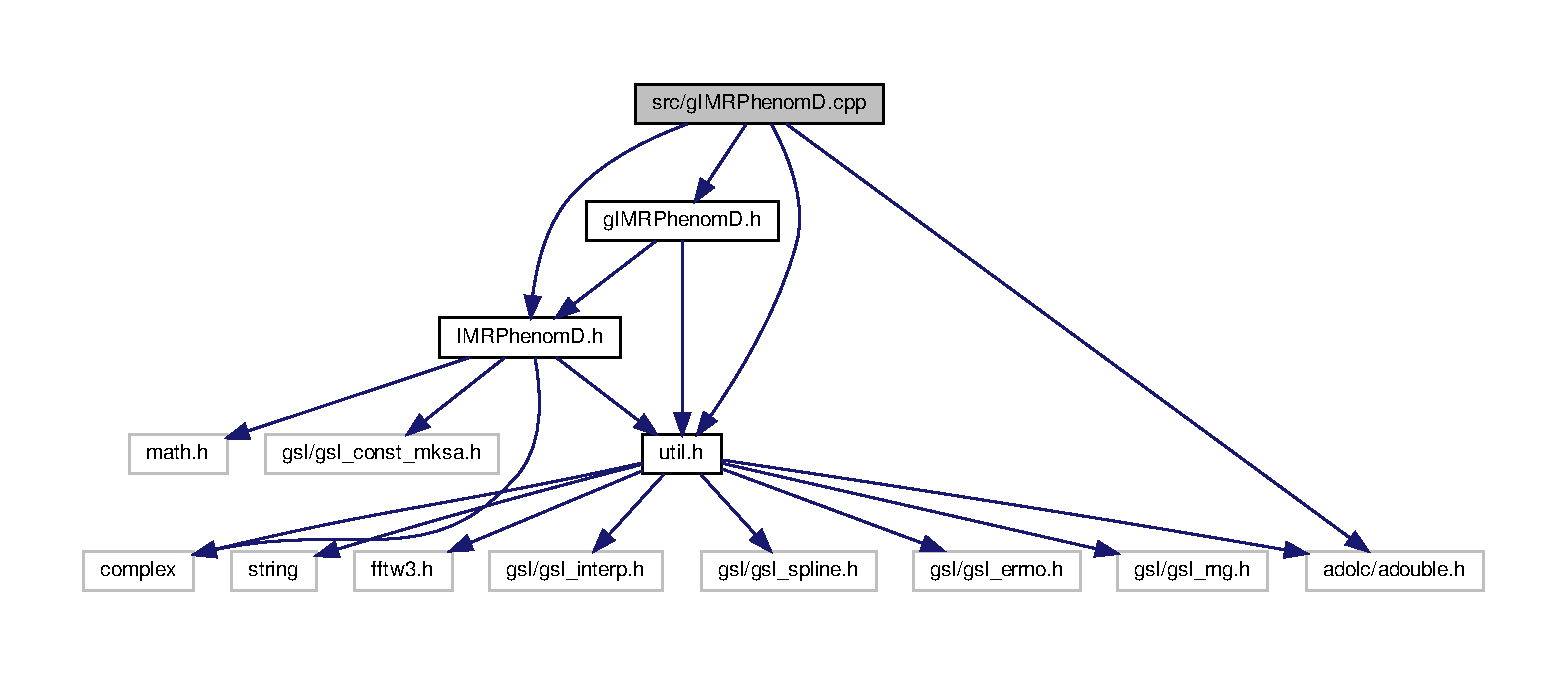
\includegraphics[width=350pt]{gIMRPhenomD_8cpp__incl}
\end{center}
\end{figure}


\doxysubsection{Detailed Description}
g\+I\+MR parameterization for modifications to GR

four groups -- phi, beta, sigma, alpha

beta can be 2,3

alpha can be 2,3,4

sigma can be 2,3,4

phi can be -\/4-\/9 (8, 9 correspond to the logarithmic terms at 5 and 6) 
\hypertarget{IMRPhenomD_8cpp}{}\doxysection{src/\+I\+M\+R\+PhenomD.cpp File Reference}
\label{IMRPhenomD_8cpp}\index{src/IMRPhenomD.cpp@{src/IMRPhenomD.cpp}}
{\ttfamily \#include \char`\"{}I\+M\+R\+Phenom\+D.\+h\char`\"{}}\newline
{\ttfamily \#include \char`\"{}Q\+N\+M\+\_\+data.\+h\char`\"{}}\newline
{\ttfamily \#include \char`\"{}util.\+h\char`\"{}}\newline
{\ttfamily \#include $<$math.\+h$>$}\newline
{\ttfamily \#include $<$iostream$>$}\newline
{\ttfamily \#include $<$complex$>$}\newline
{\ttfamily \#include $<$cmath$>$}\newline
{\ttfamily \#include $<$adolc/adouble.\+h$>$}\newline
{\ttfamily \#include $<$adolc/taping.\+h$>$}\newline
{\ttfamily \#include $<$adolc/drivers/drivers.\+h$>$}\newline
{\ttfamily \#include $<$typeinfo$>$}\newline
{\ttfamily \#include $<$omp.\+h$>$}\newline
{\ttfamily \#include $<$gsl/gsl\+\_\+interp.\+h$>$}\newline
{\ttfamily \#include $<$gsl/gsl\+\_\+spline.\+h$>$}\newline
Include dependency graph for I\+M\+R\+Phenom\+D.\+cpp\+:
\nopagebreak
\begin{figure}[H]
\begin{center}
\leavevmode
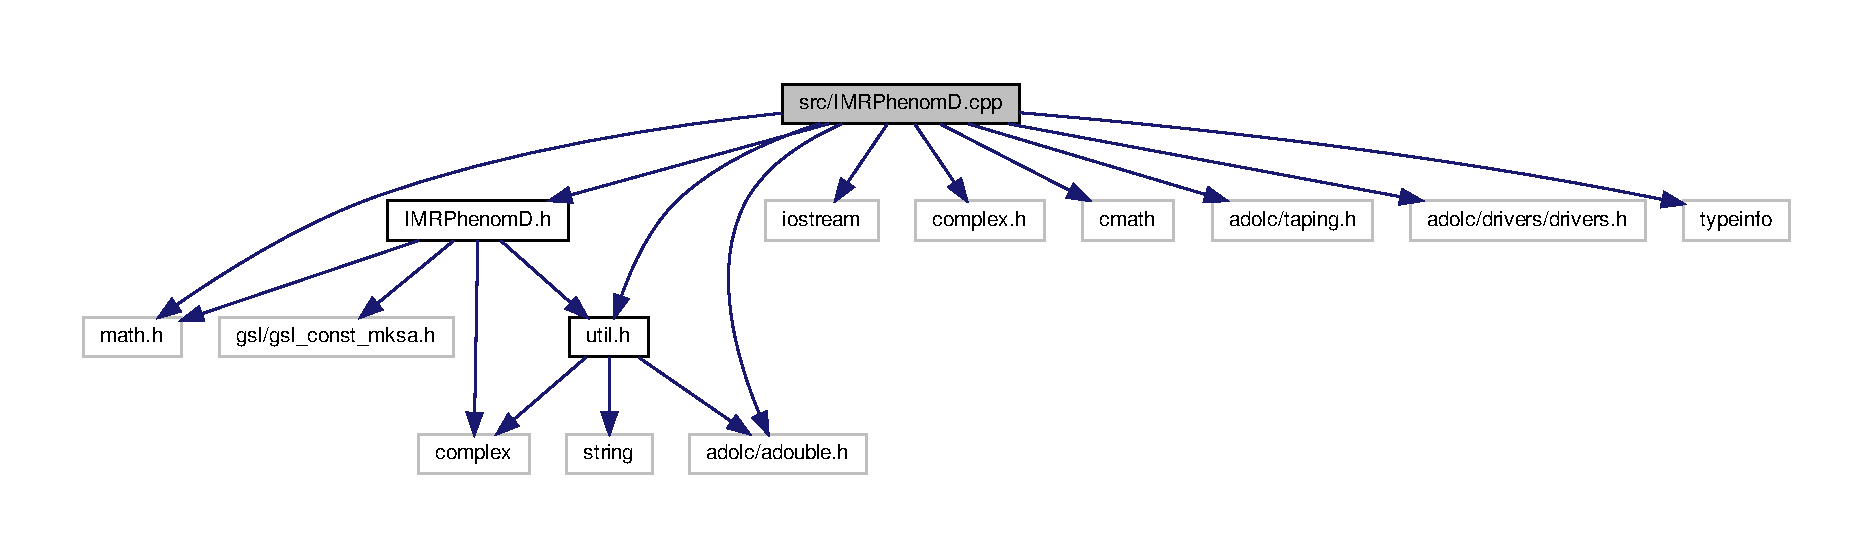
\includegraphics[width=350pt]{IMRPhenomD_8cpp__incl}
\end{center}
\end{figure}
\doxysubsection*{Macros}
\begin{DoxyCompactItemize}
\item 
\mbox{\Hypertarget{IMRPhenomD_8cpp_a71a771d0580911cb2c5fe43e369c744a}\label{IMRPhenomD_8cpp_a71a771d0580911cb2c5fe43e369c744a}} 
\#define {\bfseries omp}~ignore
\end{DoxyCompactItemize}
\doxysubsection*{Variables}
\begin{DoxyCompactItemize}
\item 
\mbox{\Hypertarget{IMRPhenomD_8cpp_a444656d90e803dcd8c71afc8d27898dd}\label{IMRPhenomD_8cpp_a444656d90e803dcd8c71afc8d27898dd}} 
double {\bfseries log\+\_\+64} = 4.\+15888308336
\end{DoxyCompactItemize}


\doxysubsection{Detailed Description}
File that includes all the low level functions that go into constructing the waveform

Matches L\+A\+Lsuite -- 2019\+\_\+09\+\_\+25

Two versions of Q\+NM fitting -- one matches L\+A\+L\+Suites\textquotesingle{} implementation, and is probably more accuate, but involves G\+SL fitting (ie not A\+D\+O\+LC friendly). The other version ensures A\+D\+O\+LC and numerical versions match -- for testing -- just comment out one option if testing (only f\+RD and fdamp) 
\hypertarget{IMRPhenomP_8cpp}{}\section{src/\+I\+M\+R\+PhenomP.cpp File Reference}
\label{IMRPhenomP_8cpp}\index{src/\+I\+M\+R\+Phenom\+P.\+cpp@{src/\+I\+M\+R\+Phenom\+P.\+cpp}}
{\ttfamily \#include \char`\"{}I\+M\+R\+Phenom\+P.\+h\char`\"{}}\newline
{\ttfamily \#include $<$iostream$>$}\newline
{\ttfamily \#include $<$fstream$>$}\newline
{\ttfamily \#include $<$string$>$}\newline
{\ttfamily \#include $<$complex$>$}\newline
{\ttfamily \#include \char`\"{}I\+M\+R\+Phenom\+D.\+h\char`\"{}}\newline
{\ttfamily \#include \char`\"{}util.\+h\char`\"{}}\newline
{\ttfamily \#include $<$adolc/adouble.\+h$>$}\newline
{\ttfamily \#include $<$math.\+h$>$}\newline
{\ttfamily \#include $<$algorithm$>$}\newline
{\ttfamily \#include $<$type\+\_\+traits$>$}\newline
{\ttfamily \#include $<$gsl/gsl\+\_\+interp.\+h$>$}\newline
{\ttfamily \#include $<$gsl/gsl\+\_\+spline.\+h$>$}\newline
Include dependency graph for I\+M\+R\+Phenom\+P.\+cpp\+:\nopagebreak
\begin{figure}[H]
\begin{center}
\leavevmode
\includegraphics[width=350pt]{IMRPhenomP_8cpp__incl}
\end{center}
\end{figure}
\subsection*{Macros}
\begin{DoxyCompactItemize}
\item 
\#define {\bfseries R\+O\+T\+A\+T\+EZ}(angle,  vx,  vy,  vz)
\item 
\#define {\bfseries R\+O\+T\+A\+T\+EY}(angle,  vx,  vy,  vz)
\end{DoxyCompactItemize}
\subsection*{Variables}
\begin{DoxyCompactItemize}
\item 
\mbox{\Hypertarget{IMRPhenomP_8cpp_a7398490e588495f0087616921a791ede}\label{IMRPhenomP_8cpp_a7398490e588495f0087616921a791ede}} 
const double {\bfseries sqrt\+\_\+6} = 2.\+44948974278317788
\end{DoxyCompactItemize}


\subsection{Detailed Description}
Source code for I\+M\+R\+PhenomP

Verified against L\+A\+Lsuite 2019\+\_\+09\+\_\+25 

\subsection{Macro Definition Documentation}
\mbox{\Hypertarget{IMRPhenomP_8cpp_ac7b1a6a2bcd511c88405f0d1c53d6f9a}\label{IMRPhenomP_8cpp_ac7b1a6a2bcd511c88405f0d1c53d6f9a}} 
\index{I\+M\+R\+Phenom\+P.\+cpp@{I\+M\+R\+Phenom\+P.\+cpp}!R\+O\+T\+A\+T\+EY@{R\+O\+T\+A\+T\+EY}}
\index{R\+O\+T\+A\+T\+EY@{R\+O\+T\+A\+T\+EY}!I\+M\+R\+Phenom\+P.\+cpp@{I\+M\+R\+Phenom\+P.\+cpp}}
\subsubsection{\texorpdfstring{R\+O\+T\+A\+T\+EY}{ROTATEY}}
{\footnotesize\ttfamily \#define R\+O\+T\+A\+T\+EY(\begin{DoxyParamCaption}\item[{}]{angle,  }\item[{}]{vx,  }\item[{}]{vy,  }\item[{}]{vz }\end{DoxyParamCaption})}

{\bfseries Value\+:}
\begin{DoxyCode}
tmp1 = vx*cos(angle) + vz*sin(angle);\(\backslash\)
tmp2 = - vx*sin(angle) + vz*cos(angle);\(\backslash\)
vx = tmp1;\(\backslash\)
vz = tmp2
\end{DoxyCode}
\mbox{\Hypertarget{IMRPhenomP_8cpp_a31ac217bed1daa05f93845a6f9a6a211}\label{IMRPhenomP_8cpp_a31ac217bed1daa05f93845a6f9a6a211}} 
\index{I\+M\+R\+Phenom\+P.\+cpp@{I\+M\+R\+Phenom\+P.\+cpp}!R\+O\+T\+A\+T\+EZ@{R\+O\+T\+A\+T\+EZ}}
\index{R\+O\+T\+A\+T\+EZ@{R\+O\+T\+A\+T\+EZ}!I\+M\+R\+Phenom\+P.\+cpp@{I\+M\+R\+Phenom\+P.\+cpp}}
\subsubsection{\texorpdfstring{R\+O\+T\+A\+T\+EZ}{ROTATEZ}}
{\footnotesize\ttfamily \#define R\+O\+T\+A\+T\+EZ(\begin{DoxyParamCaption}\item[{}]{angle,  }\item[{}]{vx,  }\item[{}]{vy,  }\item[{}]{vz }\end{DoxyParamCaption})}

{\bfseries Value\+:}
\begin{DoxyCode}
tmp1 = vx*cos(angle) - vy*sin(angle);\(\backslash\)
tmp2 = vx*sin(angle) + vy*cos(angle);\(\backslash\)
vx = tmp1;\(\backslash\)
vy = tmp2
\end{DoxyCode}

\hypertarget{io__util_8cpp}{}\doxysection{src/io\+\_\+util.cpp File Reference}
\label{io__util_8cpp}\index{src/io\_util.cpp@{src/io\_util.cpp}}
{\ttfamily \#include \char`\"{}io\+\_\+util.\+h\char`\"{}}\newline
{\ttfamily \#include \char`\"{}util.\+h\char`\"{}}\newline
{\ttfamily \#include $<$unordered\+\_\+map$>$}\newline
{\ttfamily \#include $<$string$>$}\newline
{\ttfamily \#include $<$fstream$>$}\newline
{\ttfamily \#include $<$sstream$>$}\newline
{\ttfamily \#include $<$iostream$>$}\newline
{\ttfamily \#include $<$algorithm$>$}\newline
{\ttfamily \#include $<$cctype$>$}\newline
{\ttfamily \#include $<$complex$>$}\newline
Include dependency graph for io\+\_\+util.\+cpp\+:
\nopagebreak
\begin{figure}[H]
\begin{center}
\leavevmode
\includegraphics[width=350pt]{io__util_8cpp__incl}
\end{center}
\end{figure}
\doxysubsection*{Functions}
\begin{DoxyCompactItemize}
\item 
\mbox{\Hypertarget{io__util_8cpp_ae64c41a8d5a46054427d281f7febf234}\label{io__util_8cpp_ae64c41a8d5a46054427d281f7febf234}} 
int {\bfseries unpack\+\_\+input\+\_\+io\+\_\+file} (std\+::string input\+\_\+param\+\_\+file, std\+::unordered\+\_\+map$<$ std\+::string, int $>$ $\ast$input\+\_\+param\+\_\+dict\+\_\+int, std\+::unordered\+\_\+map$<$ std\+::string, std\+::string $>$ $\ast$input\+\_\+param\+\_\+dict\+\_\+str, std\+::unordered\+\_\+map$<$ std\+::string, double $>$ $\ast$input\+\_\+param\+\_\+dict\+\_\+dbl, std\+::unordered\+\_\+map$<$ std\+::string, float $>$ $\ast$input\+\_\+param\+\_\+dict\+\_\+flt, std\+::unordered\+\_\+map$<$ std\+::string, bool $>$ $\ast$input\+\_\+param\+\_\+dict\+\_\+bool)
\item 
int \mbox{\hyperlink{io__util_8cpp_a627ac895351aa8f4c26a2565cf1769d0}{find\+\_\+datatype}} (std\+::string type)
\begin{DoxyCompactList}\small\item\em Takes in the shorthand for primitive datatypes in c++ and returns code based on type. \end{DoxyCompactList}\item 
\mbox{\Hypertarget{io__util_8cpp_a9b855aac79a01bc69b093a4ee12bb688}\label{io__util_8cpp_a9b855aac79a01bc69b093a4ee12bb688}} 
std\+::string {\bfseries trim} (std\+::string str)
\item 
void \mbox{\hyperlink{io__util_8cpp_aad742282a09bb261d21080e8874578ba}{read\+\_\+file}} (std\+::string filename, double $\ast$$\ast$output, int rows, int cols)
\begin{DoxyCompactList}\small\item\em Utility to read in data. \end{DoxyCompactList}\item 
void \mbox{\hyperlink{io__util_8cpp_a788a44b839a09910024159d9d10764d0}{read\+\_\+file}} (std\+::string filename, double $\ast$output)
\begin{DoxyCompactList}\small\item\em Utility to read in data (single dimension vector) \end{DoxyCompactList}\item 
void \mbox{\hyperlink{io__util_8cpp_a8cb10f1eb5598be2a3aa53dcc2ebe844}{write\+\_\+file}} (std\+::string filename, double $\ast$$\ast$input, int rows, int cols)
\begin{DoxyCompactList}\small\item\em Utility to write 2D array to file. \end{DoxyCompactList}\item 
void \mbox{\hyperlink{io__util_8cpp_a2364e735eddfa67c1317f6ebc64565f3}{write\+\_\+file}} (std\+::string filename, double $\ast$input, int length)
\begin{DoxyCompactList}\small\item\em Utility to write 1D array to file. \end{DoxyCompactList}\item 
void \mbox{\hyperlink{io__util_8cpp_abbb4e70ddc93c8995739b3a481bbf3a6}{read\+\_\+\+L\+O\+S\+C\+\_\+data\+\_\+file}} (std\+::string filename, double $\ast$output, double $\ast$data\+\_\+start\+\_\+time, double $\ast$duration, double $\ast$fs)
\begin{DoxyCompactList}\small\item\em Read data file from L\+I\+GO Open Science Center. \end{DoxyCompactList}\item 
void \mbox{\hyperlink{io__util_8cpp_a089aa96b136d368b0c740c416811c39d}{read\+\_\+\+L\+O\+S\+C\+\_\+\+P\+S\+D\+\_\+file}} (std\+::string filename, double $\ast$$\ast$output, int rows, int cols)
\begin{DoxyCompactList}\small\item\em Read P\+SD file from L\+I\+GO Open Science Center. \end{DoxyCompactList}\item 
void \mbox{\hyperlink{io__util_8cpp_aa73bbfc171abf859eff4c14e07ed1e0a}{allocate\+\_\+\+L\+O\+S\+C\+\_\+data}} (std\+::string $\ast$data\+\_\+files, std\+::string psd\+\_\+file, int num\+\_\+detectors, int psd\+\_\+length, int data\+\_\+file\+\_\+length, double trigger\+\_\+time, std\+::complex$<$ double $>$ $\ast$$\ast$data, double $\ast$$\ast$psds, double $\ast$$\ast$freqs)
\begin{DoxyCompactList}\small\item\em Prepare data for M\+C\+MC directly from L\+I\+GO Open Science Center. \end{DoxyCompactList}\item 
void \mbox{\hyperlink{io__util_8cpp_a3196bd767443186731edcfc84e43ac93}{free\+\_\+\+L\+O\+S\+C\+\_\+data}} (std\+::complex$<$ double $>$ $\ast$$\ast$data, double $\ast$$\ast$psds, double $\ast$$\ast$freqs, int num\+\_\+detectors, int length)
\item 
\mbox{\Hypertarget{io__util_8cpp_aabb38ec649dc87bca9ddd9ddd1baea78}\label{io__util_8cpp_aabb38ec649dc87bca9ddd9ddd1baea78}} 
int \mbox{\hyperlink{io__util_8cpp_aabb38ec649dc87bca9ddd9ddd1baea78}{count\+\_\+lines\+\_\+data\+\_\+file}} (std\+::string file, int $\ast$count)
\begin{DoxyCompactList}\small\item\em Takes in data file and returns the number of data elements in file. \end{DoxyCompactList}\item 
\mbox{\Hypertarget{io__util_8cpp_aaf15f8db5f36caf636d88f41e29b17be}\label{io__util_8cpp_aaf15f8db5f36caf636d88f41e29b17be}} 
int \mbox{\hyperlink{io__util_8cpp_aaf15f8db5f36caf636d88f41e29b17be}{count\+\_\+lines\+\_\+\+L\+O\+S\+C\+\_\+\+P\+S\+D\+\_\+file}} (std\+::string file, int $\ast$count)
\begin{DoxyCompactList}\small\item\em Takes in L\+O\+SC P\+SD file and returns the number of data elements in file. \end{DoxyCompactList}\item 
\mbox{\Hypertarget{io__util_8cpp_a2d2ec12ff7cb75ea68ec4139513bab4c}\label{io__util_8cpp_a2d2ec12ff7cb75ea68ec4139513bab4c}} 
int \mbox{\hyperlink{io__util_8cpp_a2d2ec12ff7cb75ea68ec4139513bab4c}{count\+\_\+lines\+\_\+\+L\+O\+S\+C\+\_\+data\+\_\+file}} (std\+::string file, int $\ast$count)
\begin{DoxyCompactList}\small\item\em Takes in L\+O\+SC data file and returns the number of data elements in file. \end{DoxyCompactList}\end{DoxyCompactItemize}


\doxysubsection{Detailed Description}
unpacks standard parameter file for input for runtime parameters

Returns the number of parameters unpacked, (-\/1 if error) The format M\+U\+ST be exact\+: \begin{DoxyVerb}[type] Parameter name = val

[type] Parameter name = val
\end{DoxyVerb}


The unordered\+\_\+maps contain the parameter names and are mapped to the value val

hash symbol (\#) reserved for comments

Spelling must be exact

Supported data\+\_\+types = \{int,dbl,str,flt,bool\}

If using special type, map from int to dtype separately

Trims white space on ends

Handles empty lines 

\doxysubsection{Function Documentation}
\mbox{\Hypertarget{io__util_8cpp_aa73bbfc171abf859eff4c14e07ed1e0a}\label{io__util_8cpp_aa73bbfc171abf859eff4c14e07ed1e0a}} 
\index{io\_util.cpp@{io\_util.cpp}!allocate\_LOSC\_data@{allocate\_LOSC\_data}}
\index{allocate\_LOSC\_data@{allocate\_LOSC\_data}!io\_util.cpp@{io\_util.cpp}}
\doxysubsubsection{\texorpdfstring{allocate\_LOSC\_data()}{allocate\_LOSC\_data()}}
{\footnotesize\ttfamily void allocate\+\_\+\+L\+O\+S\+C\+\_\+data (\begin{DoxyParamCaption}\item[{std\+::string $\ast$}]{data\+\_\+files,  }\item[{std\+::string}]{psd\+\_\+file,  }\item[{int}]{num\+\_\+detectors,  }\item[{int}]{psd\+\_\+length,  }\item[{int}]{data\+\_\+file\+\_\+length,  }\item[{double}]{trigger\+\_\+time,  }\item[{std\+::complex$<$ double $>$ $\ast$$\ast$}]{data,  }\item[{double $\ast$$\ast$}]{psds,  }\item[{double $\ast$$\ast$}]{freqs }\end{DoxyParamCaption})}



Prepare data for M\+C\+MC directly from L\+I\+GO Open Science Center. 

Trims data for Tobs (determined by P\+SD file) 3/4$\ast$\+Tobs in front of trigger, and 1/4$\ast$\+Tobs behind

Currently, default to sampling frequency and observation time set by P\+SD -- cannot be customized

Output is in order of P\+SD columns -- string vector of detectos M\+U\+ST match order of P\+SD cols

Output shapes-- \begin{DoxyVerb}    psds = [num_detectors][psd_length]

    data = [num_detectors][psd_length]  

    freqs = [num_detectors][psd_length] 
\end{DoxyVerb}


Total observation time = 1/( freq\mbox{[}i\mbox{]} -\/ freq\mbox{[}i-\/1\mbox{]}) (from P\+SD file)

Sampling frequency fs = max frequency from P\+SD file

A\+L\+L\+O\+C\+A\+T\+ES M\+E\+M\+O\+RY -- must be freed to prevent memory leak 
\begin{DoxyParams}[1]{Parameters}
 & {\em data\+\_\+files} & Vector of strings for each detector file from L\+O\+SC \\
\hline
 & {\em psd\+\_\+file} & String of psd file from L\+O\+SC \\
\hline
 & {\em num\+\_\+detectors} & Number of detectors to use \\
\hline
 & {\em psd\+\_\+length} & Length of the P\+SD file (number of rows of D\+A\+TA) \\
\hline
 & {\em data\+\_\+file\+\_\+length} & Length of the data file (number of rows of D\+A\+TA) \\
\hline
 & {\em trigger\+\_\+time} & Time for the signal trigger (G\+PS) \\
\hline
\mbox{\texttt{ out}}  & {\em data} & Output array of data for each detector \\
\hline
\mbox{\texttt{ out}}  & {\em psds} & Output array of psds for each detector \\
\hline
\mbox{\texttt{ out}}  & {\em freqs} & Output array of freqs for each detector \\
\hline
\end{DoxyParams}
\mbox{\Hypertarget{io__util_8cpp_a627ac895351aa8f4c26a2565cf1769d0}\label{io__util_8cpp_a627ac895351aa8f4c26a2565cf1769d0}} 
\index{io\_util.cpp@{io\_util.cpp}!find\_datatype@{find\_datatype}}
\index{find\_datatype@{find\_datatype}!io\_util.cpp@{io\_util.cpp}}
\doxysubsubsection{\texorpdfstring{find\_datatype()}{find\_datatype()}}
{\footnotesize\ttfamily int find\+\_\+datatype (\begin{DoxyParamCaption}\item[{std\+::string}]{type }\end{DoxyParamCaption})}



Takes in the shorthand for primitive datatypes in c++ and returns code based on type. 

Returns\+: \begin{DoxyVerb}0 -- Not found

1 -- int

2 -- string

3 -- double

4 -- float

5 -- bool
\end{DoxyVerb}
 \mbox{\Hypertarget{io__util_8cpp_a3196bd767443186731edcfc84e43ac93}\label{io__util_8cpp_a3196bd767443186731edcfc84e43ac93}} 
\index{io\_util.cpp@{io\_util.cpp}!free\_LOSC\_data@{free\_LOSC\_data}}
\index{free\_LOSC\_data@{free\_LOSC\_data}!io\_util.cpp@{io\_util.cpp}}
\doxysubsubsection{\texorpdfstring{free\_LOSC\_data()}{free\_LOSC\_data()}}
{\footnotesize\ttfamily void free\+\_\+\+L\+O\+S\+C\+\_\+data (\begin{DoxyParamCaption}\item[{std\+::complex$<$ double $>$ $\ast$$\ast$}]{data,  }\item[{double $\ast$$\ast$}]{psds,  }\item[{double $\ast$$\ast$}]{freqs,  }\item[{int}]{num\+\_\+detectors,  }\item[{int}]{length }\end{DoxyParamCaption})}

/brief Free data allocated by prep\+\_\+\+L\+O\+S\+C\+\_\+data function \mbox{\Hypertarget{io__util_8cpp_aad742282a09bb261d21080e8874578ba}\label{io__util_8cpp_aad742282a09bb261d21080e8874578ba}} 
\index{io\_util.cpp@{io\_util.cpp}!read\_file@{read\_file}}
\index{read\_file@{read\_file}!io\_util.cpp@{io\_util.cpp}}
\doxysubsubsection{\texorpdfstring{read\_file()}{read\_file()}\hspace{0.1cm}{\footnotesize\ttfamily [1/2]}}
{\footnotesize\ttfamily void read\+\_\+file (\begin{DoxyParamCaption}\item[{std\+::string}]{filename,  }\item[{double $\ast$$\ast$}]{output,  }\item[{int}]{rows,  }\item[{int}]{cols }\end{DoxyParamCaption})}



Utility to read in data. 

Takes filename, and assigns to output\mbox{[}rows\mbox{]}\mbox{[}cols\mbox{]}

File must be comma separated doubles 
\begin{DoxyParams}[1]{Parameters}
 & {\em filename} & input filename, relative to execution directory \\
\hline
\mbox{\texttt{ out}}  & {\em output} & array to store output, dimensions rows\+Xcols \\
\hline
 & {\em rows} & first dimension \\
\hline
 & {\em cols} & second dimension \\
\hline
\end{DoxyParams}
\mbox{\Hypertarget{io__util_8cpp_a788a44b839a09910024159d9d10764d0}\label{io__util_8cpp_a788a44b839a09910024159d9d10764d0}} 
\index{io\_util.cpp@{io\_util.cpp}!read\_file@{read\_file}}
\index{read\_file@{read\_file}!io\_util.cpp@{io\_util.cpp}}
\doxysubsubsection{\texorpdfstring{read\_file()}{read\_file()}\hspace{0.1cm}{\footnotesize\ttfamily [2/2]}}
{\footnotesize\ttfamily void read\+\_\+file (\begin{DoxyParamCaption}\item[{std\+::string}]{filename,  }\item[{double $\ast$}]{output }\end{DoxyParamCaption})}



Utility to read in data (single dimension vector) 

Takes filename, and assigns to output\mbox{[}i$\ast$rows + cols\mbox{]}

Output vector must be long enough, no check is done for the length

File must be comma separated doubles 
\begin{DoxyParams}[1]{Parameters}
 & {\em filename} & input filename, relative to execution directory \\
\hline
\mbox{\texttt{ out}}  & {\em output} & output array, assumed to have the proper length of total items \\
\hline
\end{DoxyParams}
\mbox{\Hypertarget{io__util_8cpp_abbb4e70ddc93c8995739b3a481bbf3a6}\label{io__util_8cpp_abbb4e70ddc93c8995739b3a481bbf3a6}} 
\index{io\_util.cpp@{io\_util.cpp}!read\_LOSC\_data\_file@{read\_LOSC\_data\_file}}
\index{read\_LOSC\_data\_file@{read\_LOSC\_data\_file}!io\_util.cpp@{io\_util.cpp}}
\doxysubsubsection{\texorpdfstring{read\_LOSC\_data\_file()}{read\_LOSC\_data\_file()}}
{\footnotesize\ttfamily void read\+\_\+\+L\+O\+S\+C\+\_\+data\+\_\+file (\begin{DoxyParamCaption}\item[{std\+::string}]{filename,  }\item[{double $\ast$}]{output,  }\item[{double $\ast$}]{data\+\_\+start\+\_\+time,  }\item[{double $\ast$}]{duration,  }\item[{double $\ast$}]{fs }\end{DoxyParamCaption})}



Read data file from L\+I\+GO Open Science Center. 

Convenience function for cutting off the first few lines of text 
\begin{DoxyParams}[1]{Parameters}
 & {\em filename} & input filename \\
\hline
\mbox{\texttt{ out}}  & {\em output} & Output data \\
\hline
\mbox{\texttt{ out}}  & {\em data\+\_\+start\+\_\+time} & G\+PS start time of the data in file \\
\hline
\mbox{\texttt{ out}}  & {\em duration} & Duration of the signal \\
\hline
\mbox{\texttt{ out}}  & {\em fs} & Sampling frequency of the data \\
\hline
\end{DoxyParams}
\mbox{\Hypertarget{io__util_8cpp_a089aa96b136d368b0c740c416811c39d}\label{io__util_8cpp_a089aa96b136d368b0c740c416811c39d}} 
\index{io\_util.cpp@{io\_util.cpp}!read\_LOSC\_PSD\_file@{read\_LOSC\_PSD\_file}}
\index{read\_LOSC\_PSD\_file@{read\_LOSC\_PSD\_file}!io\_util.cpp@{io\_util.cpp}}
\doxysubsubsection{\texorpdfstring{read\_LOSC\_PSD\_file()}{read\_LOSC\_PSD\_file()}}
{\footnotesize\ttfamily void read\+\_\+\+L\+O\+S\+C\+\_\+\+P\+S\+D\+\_\+file (\begin{DoxyParamCaption}\item[{std\+::string}]{filename,  }\item[{double $\ast$$\ast$}]{output,  }\item[{int}]{rows,  }\item[{int}]{cols }\end{DoxyParamCaption})}



Read P\+SD file from L\+I\+GO Open Science Center. 

Convenience function for cutting off the first few lines of text \mbox{\Hypertarget{io__util_8cpp_a8cb10f1eb5598be2a3aa53dcc2ebe844}\label{io__util_8cpp_a8cb10f1eb5598be2a3aa53dcc2ebe844}} 
\index{io\_util.cpp@{io\_util.cpp}!write\_file@{write\_file}}
\index{write\_file@{write\_file}!io\_util.cpp@{io\_util.cpp}}
\doxysubsubsection{\texorpdfstring{write\_file()}{write\_file()}\hspace{0.1cm}{\footnotesize\ttfamily [1/2]}}
{\footnotesize\ttfamily void write\+\_\+file (\begin{DoxyParamCaption}\item[{std\+::string}]{filename,  }\item[{double $\ast$$\ast$}]{input,  }\item[{int}]{rows,  }\item[{int}]{cols }\end{DoxyParamCaption})}



Utility to write 2D array to file. 

Grid of data, comma separated

Grid has rows rows and cols columns 
\begin{DoxyParams}{Parameters}
{\em filename} & Filename of output file, relative to execution directory \\
\hline
{\em input} & Input 2D array pointer array\mbox{[}rows\mbox{]}\mbox{[}cols\mbox{]} \\
\hline
{\em rows} & First dimension of array \\
\hline
{\em cols} & second dimension of array \\
\hline
\end{DoxyParams}
\mbox{\Hypertarget{io__util_8cpp_a2364e735eddfa67c1317f6ebc64565f3}\label{io__util_8cpp_a2364e735eddfa67c1317f6ebc64565f3}} 
\index{io\_util.cpp@{io\_util.cpp}!write\_file@{write\_file}}
\index{write\_file@{write\_file}!io\_util.cpp@{io\_util.cpp}}
\doxysubsubsection{\texorpdfstring{write\_file()}{write\_file()}\hspace{0.1cm}{\footnotesize\ttfamily [2/2]}}
{\footnotesize\ttfamily void write\+\_\+file (\begin{DoxyParamCaption}\item[{std\+::string}]{filename,  }\item[{double $\ast$}]{input,  }\item[{int}]{length }\end{DoxyParamCaption})}



Utility to write 1D array to file. 

Single column of data 
\begin{DoxyParams}{Parameters}
{\em filename} & Filename of output file, relative to execution directory \\
\hline
{\em input} & input 1D array pointer array\mbox{[}length\mbox{]} \\
\hline
{\em length} & length of array \\
\hline
\end{DoxyParams}

\hypertarget{mc__reject_8cpp}{}\section{src/mc\+\_\+reject.cpp File Reference}
\label{mc__reject_8cpp}\index{src/mc\+\_\+reject.\+cpp@{src/mc\+\_\+reject.\+cpp}}
{\ttfamily \#include \char`\"{}mc\+\_\+reject.\+h\char`\"{}}\newline
{\ttfamily \#include \char`\"{}util.\+h\char`\"{}}\newline
{\ttfamily \#include \char`\"{}thread\+Pool.\+h\char`\"{}}\newline
{\ttfamily \#include $<$gsl/gsl\+\_\+rng.\+h$>$}\newline
{\ttfamily \#include $<$functional$>$}\newline
{\ttfamily \#include $<$gsl/gsl\+\_\+randist.\+h$>$}\newline
Include dependency graph for mc\+\_\+reject.\+cpp\+:\nopagebreak
\begin{figure}[H]
\begin{center}
\leavevmode
\includegraphics[width=350pt]{mc__reject_8cpp__incl}
\end{center}
\end{figure}
\subsection*{Functions}
\begin{DoxyCompactItemize}
\item 
void \hyperlink{mc__reject_8cpp_a8e7fcdc575532164d9f76f27102b4c9a}{parallel\+\_\+sample} (int threadid, \hyperlink{structmcr__job}{mcr\+\_\+job} job)
\begin{DoxyCompactList}\small\item\em internal routine to draw N samples \end{DoxyCompactList}\end{DoxyCompactItemize}


\subsection{Detailed Description}
Monte Carlo Rejection sampling

Distribution should be normalized to 1 

\subsection{Function Documentation}
\mbox{\Hypertarget{mc__reject_8cpp_a8e7fcdc575532164d9f76f27102b4c9a}\label{mc__reject_8cpp_a8e7fcdc575532164d9f76f27102b4c9a}} 
\index{mc\+\_\+reject.\+cpp@{mc\+\_\+reject.\+cpp}!parallel\+\_\+sample@{parallel\+\_\+sample}}
\index{parallel\+\_\+sample@{parallel\+\_\+sample}!mc\+\_\+reject.\+cpp@{mc\+\_\+reject.\+cpp}}
\subsubsection{\texorpdfstring{parallel\+\_\+sample()}{parallel\_sample()}}
{\footnotesize\ttfamily void parallel\+\_\+sample (\begin{DoxyParamCaption}\item[{int}]{threadid,  }\item[{\hyperlink{structmcr__job}{mcr\+\_\+job}}]{job }\end{DoxyParamCaption})}



internal routine to draw N samples 

Should not be called by the user

Just made this separate from the class for now for convenience 
\begin{DoxyParams}{Parameters}
{\em job} & mcr job -- see \hyperlink{mc__reject_8h}{mc\+\_\+reject.\+h} \\
\hline
\end{DoxyParams}

\hypertarget{mcmc__gw_8cpp}{}\doxysection{src/mcmc\+\_\+gw.cpp File Reference}
\label{mcmc__gw_8cpp}\index{src/mcmc\_gw.cpp@{src/mcmc\_gw.cpp}}
{\ttfamily \#include \char`\"{}mcmc\+\_\+gw.\+h\char`\"{}}\newline
{\ttfamily \#include \char`\"{}waveform\+\_\+generator.\+h\char`\"{}}\newline
{\ttfamily \#include \char`\"{}util.\+h\char`\"{}}\newline
{\ttfamily \#include \char`\"{}detector\+\_\+util.\+h\char`\"{}}\newline
{\ttfamily \#include \char`\"{}waveform\+\_\+util.\+h\char`\"{}}\newline
{\ttfamily \#include \char`\"{}fisher.\+h\char`\"{}}\newline
{\ttfamily \#include \char`\"{}mcmc\+\_\+sampler.\+h\char`\"{}}\newline
{\ttfamily \#include $<$iostream$>$}\newline
{\ttfamily \#include $<$fstream$>$}\newline
{\ttfamily \#include $<$vector$>$}\newline
{\ttfamily \#include $<$complex$>$}\newline
{\ttfamily \#include $<$fftw3.\+h$>$}\newline
{\ttfamily \#include $<$algorithm$>$}\newline
{\ttfamily \#include $<$gsl/gsl\+\_\+interp.\+h$>$}\newline
{\ttfamily \#include $<$gsl/gsl\+\_\+spline.\+h$>$}\newline
{\ttfamily \#include $<$gsl/gsl\+\_\+errno.\+h$>$}\newline
{\ttfamily \#include $<$gsl/gsl\+\_\+randist.\+h$>$}\newline
{\ttfamily \#include $<$gsl/gsl\+\_\+rng.\+h$>$}\newline
Include dependency graph for mcmc\+\_\+gw.\+cpp\+:
% FIG 0
\doxysubsection*{Functions}
\begin{DoxyCompactItemize}
\item 
double \mbox{\hyperlink{mcmc__gw_8cpp_abd627450e43bf7ef683d875d804b7503}{maximized\+\_\+coal\+\_\+log\+\_\+likelihood\+\_\+\+I\+M\+R\+PhenomD}} (double $\ast$frequencies, int length, std\+::complex$<$ double $>$ $\ast$data, double $\ast$noise, double S\+NR, double chirpmass, double symmetric\+\_\+mass\+\_\+ratio, double spin1, double spin2, bool N\+Sflag, \mbox{\hyperlink{structfftw__outline}{fftw\+\_\+outline}} $\ast$plan)
\begin{DoxyCompactList}\small\item\em Function to calculate the log Likelihood as defined by -\/1/2 (d-\/h$\vert$d-\/h) maximized over the extrinsic parameters phic and tc. \end{DoxyCompactList}\item 
double \mbox{\hyperlink{mcmc__gw_8cpp_ae78896f8e8acd8dfaff6ff33a732284a}{maximized\+\_\+coal\+\_\+log\+\_\+likelihood\+\_\+\+I\+M\+R\+PhenomD}} (double $\ast$frequencies, size\+\_\+t length, double $\ast$real\+\_\+data, double $\ast$imag\+\_\+data, double $\ast$noise, double S\+NR, double chirpmass, double symmetric\+\_\+mass\+\_\+ratio, double spin1, double spin2, bool N\+Sflag)
\item 
double \mbox{\hyperlink{mcmc__gw_8cpp_a2635acb06ca0e448854aaab3fd7037c3}{maximized\+\_\+coal\+\_\+log\+\_\+likelihood\+\_\+\+I\+M\+R\+PhenomD}} (double $\ast$frequencies, size\+\_\+t length, double $\ast$real\+\_\+data, double $\ast$imag\+\_\+data, double $\ast$noise, double S\+NR, double chirpmass, double symmetric\+\_\+mass\+\_\+ratio, double spin1, double spin2, bool N\+Sflag, \mbox{\hyperlink{structfftw__outline}{fftw\+\_\+outline}} $\ast$plan)
\item 
double \mbox{\hyperlink{mcmc__gw_8cpp_ac66db6fc5c75ee33b84a48724b4738ef}{maximized\+\_\+coal\+\_\+log\+\_\+likelihood\+\_\+\+I\+M\+R\+Phenom\+D\+\_\+\+Full\+\_\+\+Param}} (double $\ast$frequencies, int length, std\+::complex$<$ double $>$ $\ast$data, double $\ast$noise, double chirpmass, double symmetric\+\_\+mass\+\_\+ratio, double spin1, double spin2, double Luminosity\+\_\+\+Distance, double theta, double phi, double iota, bool N\+Sflag, \mbox{\hyperlink{structfftw__outline}{fftw\+\_\+outline}} $\ast$plan)
\item 
double \mbox{\hyperlink{mcmc__gw_8cpp_a2322ab4b42380145e742ad564c643874}{maximized\+\_\+coal\+\_\+log\+\_\+likelihood\+\_\+\+I\+M\+R\+Phenom\+D\+\_\+\+Full\+\_\+\+Param}} (double $\ast$frequencies, size\+\_\+t length, double $\ast$real\+\_\+data, double $\ast$imag\+\_\+data, double $\ast$noise, double chirpmass, double symmetric\+\_\+mass\+\_\+ratio, double spin1, double spin2, double Luminosity\+\_\+\+Distance, double theta, double phi, double iota, bool N\+Sflag)
\item 
double \mbox{\hyperlink{mcmc__gw_8cpp_a3fbdbcf0651bad5541eb6e366c62de23}{maximized\+\_\+coal\+\_\+log\+\_\+likelihood\+\_\+\+I\+M\+R\+Phenom\+D\+\_\+\+Full\+\_\+\+Param}} (double $\ast$frequencies, size\+\_\+t length, double $\ast$real\+\_\+data, double $\ast$imag\+\_\+data, double $\ast$noise, double chirpmass, double symmetric\+\_\+mass\+\_\+ratio, double spin1, double spin2, double Luminosity\+\_\+\+Distance, double theta, double phi, double iota, bool N\+Sflag, \mbox{\hyperlink{structfftw__outline}{fftw\+\_\+outline}} $\ast$plan)
\item 
double \mbox{\hyperlink{mcmc__gw_8cpp_a0ae3ffbe1994b8a368c130b7f552ea28}{maximized\+\_\+\+Log\+\_\+\+Likelihood}} (std\+::complex$<$ double $>$ $\ast$data, double $\ast$psd, double $\ast$frequencies, size\+\_\+t length, \mbox{\hyperlink{classgen__params__base}{gen\+\_\+params\+\_\+base}}$<$ double $>$ $\ast$params, std\+::string detector, std\+::string generation\+\_\+method, \mbox{\hyperlink{structfftw__outline}{fftw\+\_\+outline}} $\ast$plan)
\begin{DoxyCompactList}\small\item\em routine to maximize over all extrinsic quantities and return the log likelihood \end{DoxyCompactList}\item 
\mbox{\Hypertarget{mcmc__gw_8cpp_ad7c52a57384919260f854ee553dfe554}\label{mcmc__gw_8cpp_ad7c52a57384919260f854ee553dfe554}} 
double {\bfseries maximized\+\_\+\+Log\+\_\+\+Likelihood} (double $\ast$data\+\_\+real, double $\ast$data\+\_\+imag, double $\ast$psd, double $\ast$frequencies, size\+\_\+t length, \mbox{\hyperlink{classgen__params__base}{gen\+\_\+params\+\_\+base}}$<$ double $>$ $\ast$params, std\+::string detector, std\+::string generation\+\_\+method, \mbox{\hyperlink{structfftw__outline}{fftw\+\_\+outline}} $\ast$plan)
\item 
double \mbox{\hyperlink{mcmc__gw_8cpp_ae6cc4bb69ba72e0e49a53042cfecaffe}{maximized\+\_\+coal\+\_\+\+Log\+\_\+\+Likelihood}} (std\+::complex$<$ double $>$ $\ast$data, double $\ast$psd, double $\ast$frequencies, size\+\_\+t length, \mbox{\hyperlink{classgen__params__base}{gen\+\_\+params\+\_\+base}}$<$ double $>$ $\ast$params, std\+::string detector, std\+::string generation\+\_\+method, \mbox{\hyperlink{structfftw__outline}{fftw\+\_\+outline}} $\ast$plan, double $\ast$tc, double $\ast$phic)
\begin{DoxyCompactList}\small\item\em Function to maximize only over coalescence variables tc and phic, returns the maximum values used. \end{DoxyCompactList}\item 
\mbox{\Hypertarget{mcmc__gw_8cpp_a5ad93847e3371aebb5ec16cdc98e2e4a}\label{mcmc__gw_8cpp_a5ad93847e3371aebb5ec16cdc98e2e4a}} 
double {\bfseries maximized\+\_\+coal\+\_\+\+Log\+\_\+\+Likelihood\+\_\+internal} (std\+::complex$<$ double $>$ $\ast$data, double $\ast$psd, double $\ast$frequencies, std\+::complex$<$ double $>$ $\ast$detector\+\_\+response, size\+\_\+t length, \mbox{\hyperlink{structfftw__outline}{fftw\+\_\+outline}} $\ast$plan, double $\ast$tc, double $\ast$phic)
\item 
double \mbox{\hyperlink{mcmc__gw_8cpp_ac631d3718500bb00b10e14e4d5e62adf}{Log\+\_\+\+Likelihood}} (std\+::complex$<$ double $>$ $\ast$data, double $\ast$psd, double $\ast$frequencies, size\+\_\+t length, \mbox{\hyperlink{classgen__params__base}{gen\+\_\+params\+\_\+base}}$<$ double $>$ $\ast$params, std\+::string detector, std\+::string generation\+\_\+method, \mbox{\hyperlink{structfftw__outline}{fftw\+\_\+outline}} $\ast$plan)
\begin{DoxyCompactList}\small\item\em Unmarginalized log of the likelihood. \end{DoxyCompactList}\item 
double \mbox{\hyperlink{mcmc__gw_8cpp_aecba6e7ba4f5a7463c95e0d65cfb3145}{maximized\+\_\+\+Log\+\_\+\+Likelihood\+\_\+aligned\+\_\+spin\+\_\+internal}} (std\+::complex$<$ double $>$ $\ast$data, double $\ast$psd, double $\ast$frequencies, std\+::complex$<$ double $>$ $\ast$detector\+\_\+response, size\+\_\+t length, \mbox{\hyperlink{structfftw__outline}{fftw\+\_\+outline}} $\ast$plan)
\begin{DoxyCompactList}\small\item\em Maximized match over coalescence variables -\/ returns log likelihood N\+OT N\+O\+R\+M\+A\+L\+I\+Z\+ED for aligned spins. \end{DoxyCompactList}\item 
double \mbox{\hyperlink{mcmc__gw_8cpp_a2c44e4b3acd713ae4ad07b92b96ac017}{maximized\+\_\+\+Log\+\_\+\+Likelihood\+\_\+unaligned\+\_\+spin\+\_\+internal}} (std\+::complex$<$ double $>$ $\ast$data, double $\ast$psd, double $\ast$frequencies, std\+::complex$<$ double $>$ $\ast$hplus, std\+::complex$<$ double $>$ $\ast$hcross, size\+\_\+t length, \mbox{\hyperlink{structfftw__outline}{fftw\+\_\+outline}} $\ast$plan)
\begin{DoxyCompactList}\small\item\em log likelihood function that maximizes over extrinsic parameters tc, phic, D, and phi\+Ref, the reference frequency -\/ for unaligned spins \end{DoxyCompactList}\item 
double \mbox{\hyperlink{mcmc__gw_8cpp_a5590d975e10f08888ae8b35340443b65}{Log\+\_\+\+Likelihood\+\_\+internal}} (std\+::complex$<$ double $>$ $\ast$data, double $\ast$psd, double $\ast$frequencies, std\+::complex$<$ double $>$ $\ast$detector\+\_\+response, int length, \mbox{\hyperlink{structfftw__outline}{fftw\+\_\+outline}} $\ast$plan)
\begin{DoxyCompactList}\small\item\em Internal function for the unmarginalized log of the likelihood. \end{DoxyCompactList}\item 
void \mbox{\hyperlink{mcmc__gw_8cpp_a79282d2ebb680bf028fcfc2a2e75b539}{continue\+\_\+\+R\+J\+P\+T\+M\+C\+M\+C\+\_\+\+M\+H\+\_\+\+GW}} (std\+::string start\+\_\+checkpoint\+\_\+file, double $\ast$$\ast$$\ast$output, int $\ast$$\ast$$\ast$status, int max\+\_\+dim, int min\+\_\+dim, int N\+\_\+steps, int swp\+\_\+freq, double($\ast$log\+\_\+prior)(double $\ast$param, int $\ast$status, int dimension, int chain\+\_\+id, void $\ast$parameters), void($\ast$R\+J\+\_\+proposal)(double $\ast$current\+\_\+param, double $\ast$proposed\+\_\+param, int $\ast$current\+\_\+status, int $\ast$proposed\+\_\+status, int max\+\_\+dim, int chain\+\_\+id, double step\+\_\+width, void $\ast$parameters), int num\+Threads, bool pool, bool show\+\_\+prog, int num\+\_\+detectors, std\+::complex$<$ double $>$ $\ast$$\ast$data, double $\ast$$\ast$noise\+\_\+psd, double $\ast$$\ast$frequencies, int $\ast$data\+\_\+length, double gps\+\_\+time, std\+::string $\ast$detectors, int Nmod, int $\ast$bppe, std\+::string generation\+\_\+method, std\+::string statistics\+\_\+filename, std\+::string chain\+\_\+filename, std\+::string auto\+\_\+corr\+\_\+filename, std\+::string likelihood\+\_\+log\+\_\+filename, std\+::string final\+\_\+checkpoint\+\_\+filename)
\begin{DoxyCompactList}\small\item\em Takes in an M\+C\+MC checkpoint file and continues the chain. \end{DoxyCompactList}\item 
void \mbox{\hyperlink{mcmc__gw_8cpp_a5afb8944ee754bfb6894a8c5f274553f}{R\+J\+P\+T\+M\+C\+M\+C\+\_\+\+M\+H\+\_\+\+GW}} (double $\ast$$\ast$$\ast$output, int $\ast$$\ast$$\ast$status, int max\+\_\+dim, int min\+\_\+dim, int N\+\_\+steps, int chain\+\_\+N, double $\ast$initial\+\_\+pos, int $\ast$initial\+\_\+status, double $\ast$seeding\+\_\+var, double $\ast$chain\+\_\+temps, int swp\+\_\+freq, double($\ast$log\+\_\+prior)(double $\ast$param, int $\ast$status, int dimension, int chain\+\_\+id, void $\ast$parameters), void($\ast$R\+J\+\_\+proposal)(double $\ast$current\+\_\+param, double $\ast$proposed\+\_\+param, int $\ast$current\+\_\+status, int $\ast$proposed\+\_\+status, int max\+\_\+dim, int chain\+\_\+id, double step\+\_\+width, void $\ast$parameters), int num\+Threads, bool pool, bool show\+\_\+prog, int num\+\_\+detectors, std\+::complex$<$ double $>$ $\ast$$\ast$data, double $\ast$$\ast$noise\+\_\+psd, double $\ast$$\ast$frequencies, int $\ast$data\+\_\+length, double gps\+\_\+time, std\+::string $\ast$detectors, int Nmod\+\_\+max, int $\ast$bppe, std\+::string generation\+\_\+method, std\+::string statistics\+\_\+filename, std\+::string chain\+\_\+filename, std\+::string auto\+\_\+corr\+\_\+filename, std\+::string likelihood\+\_\+log\+\_\+filename, std\+::string checkpoint\+\_\+file)
\begin{DoxyCompactList}\small\item\em Wrapper for the R\+J\+P\+T\+M\+C\+M\+C\+\_\+\+MH function, specifically for GW analysis. \end{DoxyCompactList}\item 
void \mbox{\hyperlink{mcmc__gw_8cpp_a6ca0efb402fc7c541f018dabfb2c2c10}{P\+T\+M\+C\+M\+C\+\_\+\+M\+H\+\_\+\+GW}} (double $\ast$$\ast$$\ast$output, int dimension, int N\+\_\+steps, int chain\+\_\+N, double $\ast$initial\+\_\+pos, double $\ast$seeding\+\_\+var, double $\ast$chain\+\_\+temps, int swp\+\_\+freq, double($\ast$log\+\_\+prior)(double $\ast$param, int dimension, int chain\+\_\+id, void $\ast$parameters), int num\+Threads, bool pool, bool show\+\_\+prog, int num\+\_\+detectors, std\+::complex$<$ double $>$ $\ast$$\ast$data, double $\ast$$\ast$noise\+\_\+psd, double $\ast$$\ast$frequencies, int $\ast$data\+\_\+length, double gps\+\_\+time, std\+::string $\ast$detectors, int Nmod, int $\ast$bppe, std\+::string generation\+\_\+method, std\+::string statistics\+\_\+filename, std\+::string chain\+\_\+filename, std\+::string auto\+\_\+corr\+\_\+filename, std\+::string likelihood\+\_\+log\+\_\+filename, std\+::string checkpoint\+\_\+file)
\begin{DoxyCompactList}\small\item\em Wrapper for the M\+C\+M\+C\+\_\+\+MH function, specifically for GW analysis. \end{DoxyCompactList}\item 
void \mbox{\hyperlink{mcmc__gw_8cpp_a810de43cfcb8a71ee343bfea775d59b0}{P\+T\+M\+C\+M\+C\+\_\+\+M\+H\+\_\+dynamic\+\_\+\+P\+T\+\_\+alloc\+\_\+uncorrelated\+\_\+\+GW}} (double $\ast$$\ast$output, int dimension, int N\+\_\+steps, int chain\+\_\+N, int max\+\_\+chain\+\_\+\+N\+\_\+thermo\+\_\+ensemble, double $\ast$initial\+\_\+pos, double $\ast$seeding\+\_\+var, double $\ast$chain\+\_\+temps, int swp\+\_\+freq, int t0, int nu, int corr\+\_\+threshold, int corr\+\_\+segments, double corr\+\_\+converge\+\_\+thresh, double corr\+\_\+target\+\_\+ac, std\+::string chain\+\_\+distribution\+\_\+scheme, double($\ast$log\+\_\+prior)(double $\ast$param, int dimension, int chain\+\_\+id, void $\ast$parameters), int num\+Threads, bool pool, bool show\+\_\+prog, int num\+\_\+detectors, std\+::complex$<$ double $>$ $\ast$$\ast$data, double $\ast$$\ast$noise\+\_\+psd, double $\ast$$\ast$frequencies, int $\ast$data\+\_\+length, double gps\+\_\+time, std\+::string $\ast$detectors, int Nmod, int $\ast$bppe, std\+::string generation\+\_\+method, std\+::string statistics\+\_\+filename, std\+::string chain\+\_\+filename, std\+::string likelihood\+\_\+log\+\_\+filename, std\+::string checkpoint\+\_\+filename)
\begin{DoxyCompactList}\small\item\em Takes in an M\+C\+MC checkpoint file and continues the chain. \end{DoxyCompactList}\item 
void \mbox{\hyperlink{mcmc__gw_8cpp_a70290cf146e82c84ba0b7966db67f4c2}{P\+T\+M\+C\+M\+C\+\_\+\+M\+H\+\_\+dynamic\+\_\+\+P\+T\+\_\+alloc\+\_\+\+GW}} (double $\ast$$\ast$$\ast$output, int dimension, int N\+\_\+steps, int chain\+\_\+N, int max\+\_\+chain\+\_\+\+N\+\_\+thermo\+\_\+ensemble, double $\ast$initial\+\_\+pos, double $\ast$seeding\+\_\+var, double $\ast$chain\+\_\+temps, int swp\+\_\+freq, int t0, int nu, std\+::string chain\+\_\+distribution\+\_\+scheme, double($\ast$log\+\_\+prior)(double $\ast$param, int dimension, int chain\+\_\+id, void $\ast$parameters), int num\+Threads, bool pool, bool show\+\_\+prog, int num\+\_\+detectors, std\+::complex$<$ double $>$ $\ast$$\ast$data, double $\ast$$\ast$noise\+\_\+psd, double $\ast$$\ast$frequencies, int $\ast$data\+\_\+length, double gps\+\_\+time, std\+::string $\ast$detectors, int Nmod, int $\ast$bppe, std\+::string generation\+\_\+method, std\+::string statistics\+\_\+filename, std\+::string chain\+\_\+filename, std\+::string likelihood\+\_\+log\+\_\+filename, std\+::string checkpoint\+\_\+filename)
\begin{DoxyCompactList}\small\item\em Takes in an M\+C\+MC checkpoint file and continues the chain. \end{DoxyCompactList}\item 
void \mbox{\hyperlink{mcmc__gw_8cpp_a4478b96c8918d852f3940ada3f054bdd}{continue\+\_\+\+P\+T\+M\+C\+M\+C\+\_\+\+M\+H\+\_\+\+GW}} (std\+::string start\+\_\+checkpoint\+\_\+file, double $\ast$$\ast$$\ast$output, int dimension, int N\+\_\+steps, int swp\+\_\+freq, double($\ast$log\+\_\+prior)(double $\ast$param, int dimension, int chain\+\_\+id, void $\ast$parameters), int num\+Threads, bool pool, bool show\+\_\+prog, int num\+\_\+detectors, std\+::complex$<$ double $>$ $\ast$$\ast$data, double $\ast$$\ast$noise\+\_\+psd, double $\ast$$\ast$frequencies, int $\ast$data\+\_\+length, double gps\+\_\+time, std\+::string $\ast$detectors, int Nmod, int $\ast$bppe, std\+::string generation\+\_\+method, std\+::string statistics\+\_\+filename, std\+::string chain\+\_\+filename, std\+::string auto\+\_\+corr\+\_\+filename, std\+::string likelihood\+\_\+log\+\_\+filename, std\+::string final\+\_\+checkpoint\+\_\+filename)
\begin{DoxyCompactList}\small\item\em Takes in an M\+C\+MC checkpoint file and continues the chain. \end{DoxyCompactList}\item 
void \mbox{\hyperlink{mcmc__gw_8cpp_a2e8407e705ac51ccc0e1685858ff946f}{R\+J\+P\+T\+M\+C\+M\+C\+\_\+method\+\_\+specific\+\_\+prep}} (std\+::string generation\+\_\+method, int max\+\_\+dim, int min\+\_\+dim, double $\ast$seeding\+\_\+var, bool local\+\_\+seeding)
\begin{DoxyCompactList}\small\item\em Unpacks M\+C\+MC parameters for method specific initiation (RJ version) \end{DoxyCompactList}\item 
void \mbox{\hyperlink{mcmc__gw_8cpp_a419df9528f286aba805c9dfa66118441}{P\+T\+M\+C\+M\+C\+\_\+method\+\_\+specific\+\_\+prep}} (std\+::string generation\+\_\+method, int dimension, double $\ast$seeding\+\_\+var, bool local\+\_\+seeding)
\begin{DoxyCompactList}\small\item\em Unpacks M\+C\+MC parameters for method specific initiation. \end{DoxyCompactList}\item 
\mbox{\Hypertarget{mcmc__gw_8cpp_a769426335cdac23f4fbfe4fdd0338eed}\label{mcmc__gw_8cpp_a769426335cdac23f4fbfe4fdd0338eed}} 
void {\bfseries M\+C\+M\+C\+\_\+fisher\+\_\+wrapper} (double $\ast$param, int dimension, double $\ast$$\ast$output, int chain\+\_\+id, void $\ast$parameters)
\item 
\mbox{\Hypertarget{mcmc__gw_8cpp_af1f118a2aaed0150a5ccf964506420f0}\label{mcmc__gw_8cpp_af1f118a2aaed0150a5ccf964506420f0}} 
double {\bfseries M\+C\+M\+C\+\_\+likelihood\+\_\+extrinsic} (bool save\+\_\+waveform, \mbox{\hyperlink{classgen__params__base}{gen\+\_\+params\+\_\+base}}$<$ double $>$ $\ast$parameters, std\+::string generation\+\_\+method, int $\ast$data\+\_\+length, double $\ast$$\ast$frequencies, std\+::complex$<$ double $>$ $\ast$$\ast$data, double $\ast$$\ast$psd, std\+::string $\ast$detectors, \mbox{\hyperlink{structfftw__outline}{fftw\+\_\+outline}} $\ast$fftw\+\_\+plans, int num\+\_\+detectors, double RA, double D\+EC, double gps\+\_\+time)
\item 
std\+::string \mbox{\hyperlink{mcmc__gw_8cpp_a3d25fe8ffdebc05616f1e003485770ba}{M\+C\+M\+C\+\_\+prep\+\_\+params}} (double $\ast$param, double $\ast$temp\+\_\+params, \mbox{\hyperlink{classgen__params__base}{gen\+\_\+params\+\_\+base}}$<$ double $>$ $\ast$\mbox{\hyperlink{classgen__params}{gen\+\_\+params}}, int dimension, std\+::string generation\+\_\+method)
\begin{DoxyCompactList}\small\item\em utility to do M\+C\+MC specific transformations on the input param vector before passing to the repacking utillity \end{DoxyCompactList}\item 
\mbox{\Hypertarget{mcmc__gw_8cpp_a1ec03e5500b9746713dc9d089b16d2d1}\label{mcmc__gw_8cpp_a1ec03e5500b9746713dc9d089b16d2d1}} 
double {\bfseries M\+C\+M\+C\+\_\+likelihood\+\_\+wrapper} (double $\ast$param, int dimension, int chain\+\_\+id, void $\ast$parameters)
\end{DoxyCompactItemize}


\doxysubsection{Detailed Description}
Routines for implementation in M\+C\+MC algorithms specific to GW C\+BC analysis 

\doxysubsection{Function Documentation}
\mbox{\Hypertarget{mcmc__gw_8cpp_a4478b96c8918d852f3940ada3f054bdd}\label{mcmc__gw_8cpp_a4478b96c8918d852f3940ada3f054bdd}} 
\index{mcmc\_gw.cpp@{mcmc\_gw.cpp}!continue\_PTMCMC\_MH\_GW@{continue\_PTMCMC\_MH\_GW}}
\index{continue\_PTMCMC\_MH\_GW@{continue\_PTMCMC\_MH\_GW}!mcmc\_gw.cpp@{mcmc\_gw.cpp}}
\doxysubsubsection{\texorpdfstring{continue\_PTMCMC\_MH\_GW()}{continue\_PTMCMC\_MH\_GW()}}
{\footnotesize\ttfamily void continue\+\_\+\+P\+T\+M\+C\+M\+C\+\_\+\+M\+H\+\_\+\+GW (\begin{DoxyParamCaption}\item[{std\+::string}]{start\+\_\+checkpoint\+\_\+file,  }\item[{double $\ast$$\ast$$\ast$}]{output,  }\item[{int}]{dimension,  }\item[{int}]{N\+\_\+steps,  }\item[{int}]{swp\+\_\+freq,  }\item[{double($\ast$)(double $\ast$param, int dimension, int chain\+\_\+id, void $\ast$parameters)}]{log\+\_\+prior,  }\item[{int}]{num\+Threads,  }\item[{bool}]{pool,  }\item[{bool}]{show\+\_\+prog,  }\item[{int}]{num\+\_\+detectors,  }\item[{std\+::complex$<$ double $>$ $\ast$$\ast$}]{data,  }\item[{double $\ast$$\ast$}]{noise\+\_\+psd,  }\item[{double $\ast$$\ast$}]{frequencies,  }\item[{int $\ast$}]{data\+\_\+length,  }\item[{double}]{gps\+\_\+time,  }\item[{std\+::string $\ast$}]{detectors,  }\item[{int}]{Nmod,  }\item[{int $\ast$}]{bppe,  }\item[{std\+::string}]{generation\+\_\+method,  }\item[{std\+::string}]{statistics\+\_\+filename,  }\item[{std\+::string}]{chain\+\_\+filename,  }\item[{std\+::string}]{auto\+\_\+corr\+\_\+filename,  }\item[{std\+::string}]{likelihood\+\_\+log\+\_\+filename,  }\item[{std\+::string}]{final\+\_\+checkpoint\+\_\+filename }\end{DoxyParamCaption})}



Takes in an M\+C\+MC checkpoint file and continues the chain. 

Obviously, the user must be sure to correctly match the dimension, number of chains, the generation\+\_\+method, the prior function, the data, psds, freqs, and the detectors (number and name), and the gps\+\_\+time to the previous run, otherwise the behavior of the sampler is undefined.

num\+Threads and pool do not necessarily have to be the same \mbox{\Hypertarget{mcmc__gw_8cpp_a79282d2ebb680bf028fcfc2a2e75b539}\label{mcmc__gw_8cpp_a79282d2ebb680bf028fcfc2a2e75b539}} 
\index{mcmc\_gw.cpp@{mcmc\_gw.cpp}!continue\_RJPTMCMC\_MH\_GW@{continue\_RJPTMCMC\_MH\_GW}}
\index{continue\_RJPTMCMC\_MH\_GW@{continue\_RJPTMCMC\_MH\_GW}!mcmc\_gw.cpp@{mcmc\_gw.cpp}}
\doxysubsubsection{\texorpdfstring{continue\_RJPTMCMC\_MH\_GW()}{continue\_RJPTMCMC\_MH\_GW()}}
{\footnotesize\ttfamily void continue\+\_\+\+R\+J\+P\+T\+M\+C\+M\+C\+\_\+\+M\+H\+\_\+\+GW (\begin{DoxyParamCaption}\item[{std\+::string}]{start\+\_\+checkpoint\+\_\+file,  }\item[{double $\ast$$\ast$$\ast$}]{output,  }\item[{int $\ast$$\ast$$\ast$}]{status,  }\item[{int}]{max\+\_\+dim,  }\item[{int}]{min\+\_\+dim,  }\item[{int}]{N\+\_\+steps,  }\item[{int}]{swp\+\_\+freq,  }\item[{double($\ast$)(double $\ast$param, int $\ast$status, int dimension, int chain\+\_\+id, void $\ast$parameters)}]{log\+\_\+prior,  }\item[{void($\ast$)(double $\ast$current\+\_\+param, double $\ast$proposed\+\_\+param, int $\ast$current\+\_\+status, int $\ast$proposed\+\_\+status, int max\+\_\+dim, int chain\+\_\+id, double step\+\_\+width, void $\ast$parameters)}]{R\+J\+\_\+proposal,  }\item[{int}]{num\+Threads,  }\item[{bool}]{pool,  }\item[{bool}]{show\+\_\+prog,  }\item[{int}]{num\+\_\+detectors,  }\item[{std\+::complex$<$ double $>$ $\ast$$\ast$}]{data,  }\item[{double $\ast$$\ast$}]{noise\+\_\+psd,  }\item[{double $\ast$$\ast$}]{frequencies,  }\item[{int $\ast$}]{data\+\_\+length,  }\item[{double}]{gps\+\_\+time,  }\item[{std\+::string $\ast$}]{detectors,  }\item[{int}]{Nmod,  }\item[{int $\ast$}]{bppe,  }\item[{std\+::string}]{generation\+\_\+method,  }\item[{std\+::string}]{statistics\+\_\+filename,  }\item[{std\+::string}]{chain\+\_\+filename,  }\item[{std\+::string}]{auto\+\_\+corr\+\_\+filename,  }\item[{std\+::string}]{likelihood\+\_\+log\+\_\+filename,  }\item[{std\+::string}]{final\+\_\+checkpoint\+\_\+filename }\end{DoxyParamCaption})}



Takes in an M\+C\+MC checkpoint file and continues the chain. 

Obviously, the user must be sure to correctly match the dimension, number of chains, the generation\+\_\+method, the prior function, the data, psds, freqs, and the detectors (number and name), and the gps\+\_\+time to the previous run, otherwise the behavior of the sampler is undefined.

num\+Threads and pool do not necessarily have to be the same \mbox{\Hypertarget{mcmc__gw_8cpp_ac631d3718500bb00b10e14e4d5e62adf}\label{mcmc__gw_8cpp_ac631d3718500bb00b10e14e4d5e62adf}} 
\index{mcmc\_gw.cpp@{mcmc\_gw.cpp}!Log\_Likelihood@{Log\_Likelihood}}
\index{Log\_Likelihood@{Log\_Likelihood}!mcmc\_gw.cpp@{mcmc\_gw.cpp}}
\doxysubsubsection{\texorpdfstring{Log\_Likelihood()}{Log\_Likelihood()}}
{\footnotesize\ttfamily double Log\+\_\+\+Likelihood (\begin{DoxyParamCaption}\item[{std\+::complex$<$ double $>$ $\ast$}]{data,  }\item[{double $\ast$}]{psd,  }\item[{double $\ast$}]{frequencies,  }\item[{size\+\_\+t}]{length,  }\item[{\mbox{\hyperlink{classgen__params__base}{gen\+\_\+params\+\_\+base}}$<$ double $>$ $\ast$}]{params,  }\item[{std\+::string}]{detector,  }\item[{std\+::string}]{generation\+\_\+method,  }\item[{\mbox{\hyperlink{structfftw__outline}{fftw\+\_\+outline}} $\ast$}]{plan }\end{DoxyParamCaption})}



Unmarginalized log of the likelihood. 

\mbox{\Hypertarget{mcmc__gw_8cpp_a5590d975e10f08888ae8b35340443b65}\label{mcmc__gw_8cpp_a5590d975e10f08888ae8b35340443b65}} 
\index{mcmc\_gw.cpp@{mcmc\_gw.cpp}!Log\_Likelihood\_internal@{Log\_Likelihood\_internal}}
\index{Log\_Likelihood\_internal@{Log\_Likelihood\_internal}!mcmc\_gw.cpp@{mcmc\_gw.cpp}}
\doxysubsubsection{\texorpdfstring{Log\_Likelihood\_internal()}{Log\_Likelihood\_internal()}}
{\footnotesize\ttfamily double Log\+\_\+\+Likelihood\+\_\+internal (\begin{DoxyParamCaption}\item[{std\+::complex$<$ double $>$ $\ast$}]{data,  }\item[{double $\ast$}]{psd,  }\item[{double $\ast$}]{frequencies,  }\item[{std\+::complex$<$ double $>$ $\ast$}]{detector\+\_\+response,  }\item[{int}]{length,  }\item[{\mbox{\hyperlink{structfftw__outline}{fftw\+\_\+outline}} $\ast$}]{plan }\end{DoxyParamCaption})}



Internal function for the unmarginalized log of the likelihood. 

.5 $\ast$ ( ( h $\vert$ h ) -\/ 2 ( D $\vert$ h ) ) \mbox{\Hypertarget{mcmc__gw_8cpp_ae6cc4bb69ba72e0e49a53042cfecaffe}\label{mcmc__gw_8cpp_ae6cc4bb69ba72e0e49a53042cfecaffe}} 
\index{mcmc\_gw.cpp@{mcmc\_gw.cpp}!maximized\_coal\_Log\_Likelihood@{maximized\_coal\_Log\_Likelihood}}
\index{maximized\_coal\_Log\_Likelihood@{maximized\_coal\_Log\_Likelihood}!mcmc\_gw.cpp@{mcmc\_gw.cpp}}
\doxysubsubsection{\texorpdfstring{maximized\_coal\_Log\_Likelihood()}{maximized\_coal\_Log\_Likelihood()}}
{\footnotesize\ttfamily double maximized\+\_\+coal\+\_\+\+Log\+\_\+\+Likelihood (\begin{DoxyParamCaption}\item[{std\+::complex$<$ double $>$ $\ast$}]{data,  }\item[{double $\ast$}]{psd,  }\item[{double $\ast$}]{frequencies,  }\item[{size\+\_\+t}]{length,  }\item[{\mbox{\hyperlink{classgen__params__base}{gen\+\_\+params\+\_\+base}}$<$ double $>$ $\ast$}]{params,  }\item[{std\+::string}]{detector,  }\item[{std\+::string}]{generation\+\_\+method,  }\item[{\mbox{\hyperlink{structfftw__outline}{fftw\+\_\+outline}} $\ast$}]{plan,  }\item[{double $\ast$}]{tc,  }\item[{double $\ast$}]{phic }\end{DoxyParamCaption})}



Function to maximize only over coalescence variables tc and phic, returns the maximum values used. 

\mbox{\Hypertarget{mcmc__gw_8cpp_abd627450e43bf7ef683d875d804b7503}\label{mcmc__gw_8cpp_abd627450e43bf7ef683d875d804b7503}} 
\index{mcmc\_gw.cpp@{mcmc\_gw.cpp}!maximized\_coal\_log\_likelihood\_IMRPhenomD@{maximized\_coal\_log\_likelihood\_IMRPhenomD}}
\index{maximized\_coal\_log\_likelihood\_IMRPhenomD@{maximized\_coal\_log\_likelihood\_IMRPhenomD}!mcmc\_gw.cpp@{mcmc\_gw.cpp}}
\doxysubsubsection{\texorpdfstring{maximized\_coal\_log\_likelihood\_IMRPhenomD()}{maximized\_coal\_log\_likelihood\_IMRPhenomD()}\hspace{0.1cm}{\footnotesize\ttfamily [1/3]}}
{\footnotesize\ttfamily double maximized\+\_\+coal\+\_\+log\+\_\+likelihood\+\_\+\+I\+M\+R\+PhenomD (\begin{DoxyParamCaption}\item[{double $\ast$}]{frequencies,  }\item[{int}]{length,  }\item[{std\+::complex$<$ double $>$ $\ast$}]{data,  }\item[{double $\ast$}]{noise,  }\item[{double}]{S\+NR,  }\item[{double}]{chirpmass,  }\item[{double}]{symmetric\+\_\+mass\+\_\+ratio,  }\item[{double}]{spin1,  }\item[{double}]{spin2,  }\item[{bool}]{N\+Sflag,  }\item[{\mbox{\hyperlink{structfftw__outline}{fftw\+\_\+outline}} $\ast$}]{plan }\end{DoxyParamCaption})}



Function to calculate the log Likelihood as defined by -\/1/2 (d-\/h$\vert$d-\/h) maximized over the extrinsic parameters phic and tc. 

frequency array must be uniform spacing -\/ this shouldn\textquotesingle{}t be a problem when working with real data as D\+FT return uniform spacing 
\begin{DoxyParams}{Parameters}
{\em chirpmass} & in solar masses \\
\hline
\end{DoxyParams}
\mbox{\Hypertarget{mcmc__gw_8cpp_ae78896f8e8acd8dfaff6ff33a732284a}\label{mcmc__gw_8cpp_ae78896f8e8acd8dfaff6ff33a732284a}} 
\index{mcmc\_gw.cpp@{mcmc\_gw.cpp}!maximized\_coal\_log\_likelihood\_IMRPhenomD@{maximized\_coal\_log\_likelihood\_IMRPhenomD}}
\index{maximized\_coal\_log\_likelihood\_IMRPhenomD@{maximized\_coal\_log\_likelihood\_IMRPhenomD}!mcmc\_gw.cpp@{mcmc\_gw.cpp}}
\doxysubsubsection{\texorpdfstring{maximized\_coal\_log\_likelihood\_IMRPhenomD()}{maximized\_coal\_log\_likelihood\_IMRPhenomD()}\hspace{0.1cm}{\footnotesize\ttfamily [2/3]}}
{\footnotesize\ttfamily double maximized\+\_\+coal\+\_\+log\+\_\+likelihood\+\_\+\+I\+M\+R\+PhenomD (\begin{DoxyParamCaption}\item[{double $\ast$}]{frequencies,  }\item[{size\+\_\+t}]{length,  }\item[{double $\ast$}]{real\+\_\+data,  }\item[{double $\ast$}]{imag\+\_\+data,  }\item[{double $\ast$}]{noise,  }\item[{double}]{S\+NR,  }\item[{double}]{chirpmass,  }\item[{double}]{symmetric\+\_\+mass\+\_\+ratio,  }\item[{double}]{spin1,  }\item[{double}]{spin2,  }\item[{bool}]{N\+Sflag }\end{DoxyParamCaption})}


\begin{DoxyParams}{Parameters}
{\em chirpmass} & in solar masses \\
\hline
\end{DoxyParams}
\mbox{\Hypertarget{mcmc__gw_8cpp_a2635acb06ca0e448854aaab3fd7037c3}\label{mcmc__gw_8cpp_a2635acb06ca0e448854aaab3fd7037c3}} 
\index{mcmc\_gw.cpp@{mcmc\_gw.cpp}!maximized\_coal\_log\_likelihood\_IMRPhenomD@{maximized\_coal\_log\_likelihood\_IMRPhenomD}}
\index{maximized\_coal\_log\_likelihood\_IMRPhenomD@{maximized\_coal\_log\_likelihood\_IMRPhenomD}!mcmc\_gw.cpp@{mcmc\_gw.cpp}}
\doxysubsubsection{\texorpdfstring{maximized\_coal\_log\_likelihood\_IMRPhenomD()}{maximized\_coal\_log\_likelihood\_IMRPhenomD()}\hspace{0.1cm}{\footnotesize\ttfamily [3/3]}}
{\footnotesize\ttfamily double maximized\+\_\+coal\+\_\+log\+\_\+likelihood\+\_\+\+I\+M\+R\+PhenomD (\begin{DoxyParamCaption}\item[{double $\ast$}]{frequencies,  }\item[{size\+\_\+t}]{length,  }\item[{double $\ast$}]{real\+\_\+data,  }\item[{double $\ast$}]{imag\+\_\+data,  }\item[{double $\ast$}]{noise,  }\item[{double}]{S\+NR,  }\item[{double}]{chirpmass,  }\item[{double}]{symmetric\+\_\+mass\+\_\+ratio,  }\item[{double}]{spin1,  }\item[{double}]{spin2,  }\item[{bool}]{N\+Sflag,  }\item[{\mbox{\hyperlink{structfftw__outline}{fftw\+\_\+outline}} $\ast$}]{plan }\end{DoxyParamCaption})}


\begin{DoxyParams}{Parameters}
{\em chirpmass} & in solar masses \\
\hline
\end{DoxyParams}
\mbox{\Hypertarget{mcmc__gw_8cpp_ac66db6fc5c75ee33b84a48724b4738ef}\label{mcmc__gw_8cpp_ac66db6fc5c75ee33b84a48724b4738ef}} 
\index{mcmc\_gw.cpp@{mcmc\_gw.cpp}!maximized\_coal\_log\_likelihood\_IMRPhenomD\_Full\_Param@{maximized\_coal\_log\_likelihood\_IMRPhenomD\_Full\_Param}}
\index{maximized\_coal\_log\_likelihood\_IMRPhenomD\_Full\_Param@{maximized\_coal\_log\_likelihood\_IMRPhenomD\_Full\_Param}!mcmc\_gw.cpp@{mcmc\_gw.cpp}}
\doxysubsubsection{\texorpdfstring{maximized\_coal\_log\_likelihood\_IMRPhenomD\_Full\_Param()}{maximized\_coal\_log\_likelihood\_IMRPhenomD\_Full\_Param()}\hspace{0.1cm}{\footnotesize\ttfamily [1/3]}}
{\footnotesize\ttfamily double maximized\+\_\+coal\+\_\+log\+\_\+likelihood\+\_\+\+I\+M\+R\+Phenom\+D\+\_\+\+Full\+\_\+\+Param (\begin{DoxyParamCaption}\item[{double $\ast$}]{frequencies,  }\item[{int}]{length,  }\item[{std\+::complex$<$ double $>$ $\ast$}]{data,  }\item[{double $\ast$}]{noise,  }\item[{double}]{chirpmass,  }\item[{double}]{symmetric\+\_\+mass\+\_\+ratio,  }\item[{double}]{spin1,  }\item[{double}]{spin2,  }\item[{double}]{Luminosity\+\_\+\+Distance,  }\item[{double}]{theta,  }\item[{double}]{phi,  }\item[{double}]{iota,  }\item[{bool}]{N\+Sflag,  }\item[{\mbox{\hyperlink{structfftw__outline}{fftw\+\_\+outline}} $\ast$}]{plan }\end{DoxyParamCaption})}


\begin{DoxyParams}{Parameters}
{\em chirpmass} & in solar masses \\
\hline
\end{DoxyParams}
\mbox{\Hypertarget{mcmc__gw_8cpp_a2322ab4b42380145e742ad564c643874}\label{mcmc__gw_8cpp_a2322ab4b42380145e742ad564c643874}} 
\index{mcmc\_gw.cpp@{mcmc\_gw.cpp}!maximized\_coal\_log\_likelihood\_IMRPhenomD\_Full\_Param@{maximized\_coal\_log\_likelihood\_IMRPhenomD\_Full\_Param}}
\index{maximized\_coal\_log\_likelihood\_IMRPhenomD\_Full\_Param@{maximized\_coal\_log\_likelihood\_IMRPhenomD\_Full\_Param}!mcmc\_gw.cpp@{mcmc\_gw.cpp}}
\doxysubsubsection{\texorpdfstring{maximized\_coal\_log\_likelihood\_IMRPhenomD\_Full\_Param()}{maximized\_coal\_log\_likelihood\_IMRPhenomD\_Full\_Param()}\hspace{0.1cm}{\footnotesize\ttfamily [2/3]}}
{\footnotesize\ttfamily double maximized\+\_\+coal\+\_\+log\+\_\+likelihood\+\_\+\+I\+M\+R\+Phenom\+D\+\_\+\+Full\+\_\+\+Param (\begin{DoxyParamCaption}\item[{double $\ast$}]{frequencies,  }\item[{size\+\_\+t}]{length,  }\item[{double $\ast$}]{real\+\_\+data,  }\item[{double $\ast$}]{imag\+\_\+data,  }\item[{double $\ast$}]{noise,  }\item[{double}]{chirpmass,  }\item[{double}]{symmetric\+\_\+mass\+\_\+ratio,  }\item[{double}]{spin1,  }\item[{double}]{spin2,  }\item[{double}]{Luminosity\+\_\+\+Distance,  }\item[{double}]{theta,  }\item[{double}]{phi,  }\item[{double}]{iota,  }\item[{bool}]{N\+Sflag }\end{DoxyParamCaption})}


\begin{DoxyParams}{Parameters}
{\em chirpmass} & in solar masses \\
\hline
\end{DoxyParams}
\mbox{\Hypertarget{mcmc__gw_8cpp_a3fbdbcf0651bad5541eb6e366c62de23}\label{mcmc__gw_8cpp_a3fbdbcf0651bad5541eb6e366c62de23}} 
\index{mcmc\_gw.cpp@{mcmc\_gw.cpp}!maximized\_coal\_log\_likelihood\_IMRPhenomD\_Full\_Param@{maximized\_coal\_log\_likelihood\_IMRPhenomD\_Full\_Param}}
\index{maximized\_coal\_log\_likelihood\_IMRPhenomD\_Full\_Param@{maximized\_coal\_log\_likelihood\_IMRPhenomD\_Full\_Param}!mcmc\_gw.cpp@{mcmc\_gw.cpp}}
\doxysubsubsection{\texorpdfstring{maximized\_coal\_log\_likelihood\_IMRPhenomD\_Full\_Param()}{maximized\_coal\_log\_likelihood\_IMRPhenomD\_Full\_Param()}\hspace{0.1cm}{\footnotesize\ttfamily [3/3]}}
{\footnotesize\ttfamily double maximized\+\_\+coal\+\_\+log\+\_\+likelihood\+\_\+\+I\+M\+R\+Phenom\+D\+\_\+\+Full\+\_\+\+Param (\begin{DoxyParamCaption}\item[{double $\ast$}]{frequencies,  }\item[{size\+\_\+t}]{length,  }\item[{double $\ast$}]{real\+\_\+data,  }\item[{double $\ast$}]{imag\+\_\+data,  }\item[{double $\ast$}]{noise,  }\item[{double}]{chirpmass,  }\item[{double}]{symmetric\+\_\+mass\+\_\+ratio,  }\item[{double}]{spin1,  }\item[{double}]{spin2,  }\item[{double}]{Luminosity\+\_\+\+Distance,  }\item[{double}]{theta,  }\item[{double}]{phi,  }\item[{double}]{iota,  }\item[{bool}]{N\+Sflag,  }\item[{\mbox{\hyperlink{structfftw__outline}{fftw\+\_\+outline}} $\ast$}]{plan }\end{DoxyParamCaption})}


\begin{DoxyParams}{Parameters}
{\em chirpmass} & in solar masses \\
\hline
\end{DoxyParams}
\mbox{\Hypertarget{mcmc__gw_8cpp_a0ae3ffbe1994b8a368c130b7f552ea28}\label{mcmc__gw_8cpp_a0ae3ffbe1994b8a368c130b7f552ea28}} 
\index{mcmc\_gw.cpp@{mcmc\_gw.cpp}!maximized\_Log\_Likelihood@{maximized\_Log\_Likelihood}}
\index{maximized\_Log\_Likelihood@{maximized\_Log\_Likelihood}!mcmc\_gw.cpp@{mcmc\_gw.cpp}}
\doxysubsubsection{\texorpdfstring{maximized\_Log\_Likelihood()}{maximized\_Log\_Likelihood()}}
{\footnotesize\ttfamily double maximized\+\_\+\+Log\+\_\+\+Likelihood (\begin{DoxyParamCaption}\item[{std\+::complex$<$ double $>$ $\ast$}]{data,  }\item[{double $\ast$}]{psd,  }\item[{double $\ast$}]{frequencies,  }\item[{size\+\_\+t}]{length,  }\item[{\mbox{\hyperlink{classgen__params__base}{gen\+\_\+params\+\_\+base}}$<$ double $>$ $\ast$}]{params,  }\item[{std\+::string}]{detector,  }\item[{std\+::string}]{generation\+\_\+method,  }\item[{\mbox{\hyperlink{structfftw__outline}{fftw\+\_\+outline}} $\ast$}]{plan }\end{DoxyParamCaption})}



routine to maximize over all extrinsic quantities and return the log likelihood 

\mbox{\hyperlink{classIMRPhenomD}{I\+M\+R\+PhenomD}} -- maximizes over DL, phic, tc, \textbackslash{}iota, \textbackslash{}phi, \textbackslash{}theta I\+M\+R\+PhenomP -- maximizes over DL, phic,tc, \textbackslash{}psi, \textbackslash{}phi , \textbackslash{}theta \mbox{\Hypertarget{mcmc__gw_8cpp_aecba6e7ba4f5a7463c95e0d65cfb3145}\label{mcmc__gw_8cpp_aecba6e7ba4f5a7463c95e0d65cfb3145}} 
\index{mcmc\_gw.cpp@{mcmc\_gw.cpp}!maximized\_Log\_Likelihood\_aligned\_spin\_internal@{maximized\_Log\_Likelihood\_aligned\_spin\_internal}}
\index{maximized\_Log\_Likelihood\_aligned\_spin\_internal@{maximized\_Log\_Likelihood\_aligned\_spin\_internal}!mcmc\_gw.cpp@{mcmc\_gw.cpp}}
\doxysubsubsection{\texorpdfstring{maximized\_Log\_Likelihood\_aligned\_spin\_internal()}{maximized\_Log\_Likelihood\_aligned\_spin\_internal()}}
{\footnotesize\ttfamily double maximized\+\_\+\+Log\+\_\+\+Likelihood\+\_\+aligned\+\_\+spin\+\_\+internal (\begin{DoxyParamCaption}\item[{std\+::complex$<$ double $>$ $\ast$}]{data,  }\item[{double $\ast$}]{psd,  }\item[{double $\ast$}]{frequencies,  }\item[{std\+::complex$<$ double $>$ $\ast$}]{detector\+\_\+response,  }\item[{size\+\_\+t}]{length,  }\item[{\mbox{\hyperlink{structfftw__outline}{fftw\+\_\+outline}} $\ast$}]{plan }\end{DoxyParamCaption})}



Maximized match over coalescence variables -\/ returns log likelihood N\+OT N\+O\+R\+M\+A\+L\+I\+Z\+ED for aligned spins. 

Note\+: this function is not properly normalized for an absolute comparison. This is made for M\+C\+MC sampling, so to minimize time, constant terms like (Data$\vert$\+Data), which would cancel in the Metropolis-\/\+Hasting ratio, are left out for efficiency \mbox{\Hypertarget{mcmc__gw_8cpp_a2c44e4b3acd713ae4ad07b92b96ac017}\label{mcmc__gw_8cpp_a2c44e4b3acd713ae4ad07b92b96ac017}} 
\index{mcmc\_gw.cpp@{mcmc\_gw.cpp}!maximized\_Log\_Likelihood\_unaligned\_spin\_internal@{maximized\_Log\_Likelihood\_unaligned\_spin\_internal}}
\index{maximized\_Log\_Likelihood\_unaligned\_spin\_internal@{maximized\_Log\_Likelihood\_unaligned\_spin\_internal}!mcmc\_gw.cpp@{mcmc\_gw.cpp}}
\doxysubsubsection{\texorpdfstring{maximized\_Log\_Likelihood\_unaligned\_spin\_internal()}{maximized\_Log\_Likelihood\_unaligned\_spin\_internal()}}
{\footnotesize\ttfamily double maximized\+\_\+\+Log\+\_\+\+Likelihood\+\_\+unaligned\+\_\+spin\+\_\+internal (\begin{DoxyParamCaption}\item[{std\+::complex$<$ double $>$ $\ast$}]{data,  }\item[{double $\ast$}]{psd,  }\item[{double $\ast$}]{frequencies,  }\item[{std\+::complex$<$ double $>$ $\ast$}]{hplus,  }\item[{std\+::complex$<$ double $>$ $\ast$}]{hcross,  }\item[{size\+\_\+t}]{length,  }\item[{\mbox{\hyperlink{structfftw__outline}{fftw\+\_\+outline}} $\ast$}]{plan }\end{DoxyParamCaption})}



log likelihood function that maximizes over extrinsic parameters tc, phic, D, and phi\+Ref, the reference frequency -\/ for unaligned spins 

Ref\+: ar\+Xiv 1603.\+02444v2 \mbox{\Hypertarget{mcmc__gw_8cpp_a3d25fe8ffdebc05616f1e003485770ba}\label{mcmc__gw_8cpp_a3d25fe8ffdebc05616f1e003485770ba}} 
\index{mcmc\_gw.cpp@{mcmc\_gw.cpp}!MCMC\_prep\_params@{MCMC\_prep\_params}}
\index{MCMC\_prep\_params@{MCMC\_prep\_params}!mcmc\_gw.cpp@{mcmc\_gw.cpp}}
\doxysubsubsection{\texorpdfstring{MCMC\_prep\_params()}{MCMC\_prep\_params()}}
{\footnotesize\ttfamily std\+::string M\+C\+M\+C\+\_\+prep\+\_\+params (\begin{DoxyParamCaption}\item[{double $\ast$}]{param,  }\item[{double $\ast$}]{temp\+\_\+params,  }\item[{\mbox{\hyperlink{classgen__params__base}{gen\+\_\+params\+\_\+base}}$<$ double $>$ $\ast$}]{gen\+\_\+params,  }\item[{int}]{dimension,  }\item[{std\+::string}]{generation\+\_\+method }\end{DoxyParamCaption})}



utility to do M\+C\+MC specific transformations on the input param vector before passing to the repacking utillity 

Returns the local generation method to be used in the LL functions \mbox{\Hypertarget{mcmc__gw_8cpp_a419df9528f286aba805c9dfa66118441}\label{mcmc__gw_8cpp_a419df9528f286aba805c9dfa66118441}} 
\index{mcmc\_gw.cpp@{mcmc\_gw.cpp}!PTMCMC\_method\_specific\_prep@{PTMCMC\_method\_specific\_prep}}
\index{PTMCMC\_method\_specific\_prep@{PTMCMC\_method\_specific\_prep}!mcmc\_gw.cpp@{mcmc\_gw.cpp}}
\doxysubsubsection{\texorpdfstring{PTMCMC\_method\_specific\_prep()}{PTMCMC\_method\_specific\_prep()}}
{\footnotesize\ttfamily void P\+T\+M\+C\+M\+C\+\_\+method\+\_\+specific\+\_\+prep (\begin{DoxyParamCaption}\item[{std\+::string}]{generation\+\_\+method,  }\item[{int}]{dimension,  }\item[{double $\ast$}]{seeding\+\_\+var,  }\item[{bool}]{local\+\_\+seeding }\end{DoxyParamCaption})}



Unpacks M\+C\+MC parameters for method specific initiation. 

Populates seeding vector if non supplied, populates mcmc\+\_\+\+Nmod, populates mcmc\+\_\+log\+\_\+beta, populates mcmc\+\_\+intrinsic \mbox{\Hypertarget{mcmc__gw_8cpp_a70290cf146e82c84ba0b7966db67f4c2}\label{mcmc__gw_8cpp_a70290cf146e82c84ba0b7966db67f4c2}} 
\index{mcmc\_gw.cpp@{mcmc\_gw.cpp}!PTMCMC\_MH\_dynamic\_PT\_alloc\_GW@{PTMCMC\_MH\_dynamic\_PT\_alloc\_GW}}
\index{PTMCMC\_MH\_dynamic\_PT\_alloc\_GW@{PTMCMC\_MH\_dynamic\_PT\_alloc\_GW}!mcmc\_gw.cpp@{mcmc\_gw.cpp}}
\doxysubsubsection{\texorpdfstring{PTMCMC\_MH\_dynamic\_PT\_alloc\_GW()}{PTMCMC\_MH\_dynamic\_PT\_alloc\_GW()}}
{\footnotesize\ttfamily void P\+T\+M\+C\+M\+C\+\_\+\+M\+H\+\_\+dynamic\+\_\+\+P\+T\+\_\+alloc\+\_\+\+GW (\begin{DoxyParamCaption}\item[{double $\ast$$\ast$$\ast$}]{output,  }\item[{int}]{dimension,  }\item[{int}]{N\+\_\+steps,  }\item[{int}]{chain\+\_\+N,  }\item[{int}]{max\+\_\+chain\+\_\+\+N\+\_\+thermo\+\_\+ensemble,  }\item[{double $\ast$}]{initial\+\_\+pos,  }\item[{double $\ast$}]{seeding\+\_\+var,  }\item[{double $\ast$}]{chain\+\_\+temps,  }\item[{int}]{swp\+\_\+freq,  }\item[{int}]{t0,  }\item[{int}]{nu,  }\item[{std\+::string}]{chain\+\_\+distribution\+\_\+scheme,  }\item[{double($\ast$)(double $\ast$param, int dimension, int chain\+\_\+id, void $\ast$parameters)}]{log\+\_\+prior,  }\item[{int}]{num\+Threads,  }\item[{bool}]{pool,  }\item[{bool}]{show\+\_\+prog,  }\item[{int}]{num\+\_\+detectors,  }\item[{std\+::complex$<$ double $>$ $\ast$$\ast$}]{data,  }\item[{double $\ast$$\ast$}]{noise\+\_\+psd,  }\item[{double $\ast$$\ast$}]{frequencies,  }\item[{int $\ast$}]{data\+\_\+length,  }\item[{double}]{gps\+\_\+time,  }\item[{std\+::string $\ast$}]{detectors,  }\item[{int}]{Nmod,  }\item[{int $\ast$}]{bppe,  }\item[{std\+::string}]{generation\+\_\+method,  }\item[{std\+::string}]{statistics\+\_\+filename,  }\item[{std\+::string}]{chain\+\_\+filename,  }\item[{std\+::string}]{likelihood\+\_\+log\+\_\+filename,  }\item[{std\+::string}]{checkpoint\+\_\+filename }\end{DoxyParamCaption})}



Takes in an M\+C\+MC checkpoint file and continues the chain. 

Obviously, the user must be sure to correctly match the dimension, number of chains, the generation\+\_\+method, the prior function, the data, psds, freqs, and the detectors (number and name), and the gps\+\_\+time to the previous run, otherwise the behavior of the sampler is undefined.

num\+Threads and pool do not necessarily have to be the same \mbox{\Hypertarget{mcmc__gw_8cpp_a810de43cfcb8a71ee343bfea775d59b0}\label{mcmc__gw_8cpp_a810de43cfcb8a71ee343bfea775d59b0}} 
\index{mcmc\_gw.cpp@{mcmc\_gw.cpp}!PTMCMC\_MH\_dynamic\_PT\_alloc\_uncorrelated\_GW@{PTMCMC\_MH\_dynamic\_PT\_alloc\_uncorrelated\_GW}}
\index{PTMCMC\_MH\_dynamic\_PT\_alloc\_uncorrelated\_GW@{PTMCMC\_MH\_dynamic\_PT\_alloc\_uncorrelated\_GW}!mcmc\_gw.cpp@{mcmc\_gw.cpp}}
\doxysubsubsection{\texorpdfstring{PTMCMC\_MH\_dynamic\_PT\_alloc\_uncorrelated\_GW()}{PTMCMC\_MH\_dynamic\_PT\_alloc\_uncorrelated\_GW()}}
{\footnotesize\ttfamily void P\+T\+M\+C\+M\+C\+\_\+\+M\+H\+\_\+dynamic\+\_\+\+P\+T\+\_\+alloc\+\_\+uncorrelated\+\_\+\+GW (\begin{DoxyParamCaption}\item[{double $\ast$$\ast$}]{output,  }\item[{int}]{dimension,  }\item[{int}]{N\+\_\+steps,  }\item[{int}]{chain\+\_\+N,  }\item[{int}]{max\+\_\+chain\+\_\+\+N\+\_\+thermo\+\_\+ensemble,  }\item[{double $\ast$}]{initial\+\_\+pos,  }\item[{double $\ast$}]{seeding\+\_\+var,  }\item[{double $\ast$}]{chain\+\_\+temps,  }\item[{int}]{swp\+\_\+freq,  }\item[{int}]{t0,  }\item[{int}]{nu,  }\item[{int}]{corr\+\_\+threshold,  }\item[{int}]{corr\+\_\+segments,  }\item[{double}]{corr\+\_\+converge\+\_\+thresh,  }\item[{double}]{corr\+\_\+target\+\_\+ac,  }\item[{std\+::string}]{chain\+\_\+distribution\+\_\+scheme,  }\item[{double($\ast$)(double $\ast$param, int dimension, int chain\+\_\+id, void $\ast$parameters)}]{log\+\_\+prior,  }\item[{int}]{num\+Threads,  }\item[{bool}]{pool,  }\item[{bool}]{show\+\_\+prog,  }\item[{int}]{num\+\_\+detectors,  }\item[{std\+::complex$<$ double $>$ $\ast$$\ast$}]{data,  }\item[{double $\ast$$\ast$}]{noise\+\_\+psd,  }\item[{double $\ast$$\ast$}]{frequencies,  }\item[{int $\ast$}]{data\+\_\+length,  }\item[{double}]{gps\+\_\+time,  }\item[{std\+::string $\ast$}]{detectors,  }\item[{int}]{Nmod,  }\item[{int $\ast$}]{bppe,  }\item[{std\+::string}]{generation\+\_\+method,  }\item[{std\+::string}]{statistics\+\_\+filename,  }\item[{std\+::string}]{chain\+\_\+filename,  }\item[{std\+::string}]{likelihood\+\_\+log\+\_\+filename,  }\item[{std\+::string}]{checkpoint\+\_\+filename }\end{DoxyParamCaption})}



Takes in an M\+C\+MC checkpoint file and continues the chain. 

Obviously, the user must be sure to correctly match the dimension, number of chains, the generation\+\_\+method, the prior function, the data, psds, freqs, and the detectors (number and name), and the gps\+\_\+time to the previous run, otherwise the behavior of the sampler is undefined.

num\+Threads and pool do not necessarily have to be the same \mbox{\Hypertarget{mcmc__gw_8cpp_a6ca0efb402fc7c541f018dabfb2c2c10}\label{mcmc__gw_8cpp_a6ca0efb402fc7c541f018dabfb2c2c10}} 
\index{mcmc\_gw.cpp@{mcmc\_gw.cpp}!PTMCMC\_MH\_GW@{PTMCMC\_MH\_GW}}
\index{PTMCMC\_MH\_GW@{PTMCMC\_MH\_GW}!mcmc\_gw.cpp@{mcmc\_gw.cpp}}
\doxysubsubsection{\texorpdfstring{PTMCMC\_MH\_GW()}{PTMCMC\_MH\_GW()}}
{\footnotesize\ttfamily void P\+T\+M\+C\+M\+C\+\_\+\+M\+H\+\_\+\+GW (\begin{DoxyParamCaption}\item[{double $\ast$$\ast$$\ast$}]{output,  }\item[{int}]{dimension,  }\item[{int}]{N\+\_\+steps,  }\item[{int}]{chain\+\_\+N,  }\item[{double $\ast$}]{initial\+\_\+pos,  }\item[{double $\ast$}]{seeding\+\_\+var,  }\item[{double $\ast$}]{chain\+\_\+temps,  }\item[{int}]{swp\+\_\+freq,  }\item[{double($\ast$)(double $\ast$param, int dimension, int chain\+\_\+id, void $\ast$parameters)}]{log\+\_\+prior,  }\item[{int}]{num\+Threads,  }\item[{bool}]{pool,  }\item[{bool}]{show\+\_\+prog,  }\item[{int}]{num\+\_\+detectors,  }\item[{std\+::complex$<$ double $>$ $\ast$$\ast$}]{data,  }\item[{double $\ast$$\ast$}]{noise\+\_\+psd,  }\item[{double $\ast$$\ast$}]{frequencies,  }\item[{int $\ast$}]{data\+\_\+length,  }\item[{double}]{gps\+\_\+time,  }\item[{std\+::string $\ast$}]{detectors,  }\item[{int}]{Nmod,  }\item[{int $\ast$}]{bppe,  }\item[{std\+::string}]{generation\+\_\+method,  }\item[{std\+::string}]{statistics\+\_\+filename,  }\item[{std\+::string}]{chain\+\_\+filename,  }\item[{std\+::string}]{auto\+\_\+corr\+\_\+filename,  }\item[{std\+::string}]{likelihood\+\_\+log\+\_\+filename,  }\item[{std\+::string}]{checkpoint\+\_\+file }\end{DoxyParamCaption})}



Wrapper for the M\+C\+M\+C\+\_\+\+MH function, specifically for GW analysis. 

Handles the details of setting up the M\+C\+MC sampler and wraps the fisher and log likelihood to conform to the format of the sampler

{\itshape N\+O\+TE} -- This sampler is N\+OT thread safe. There is global memory declared for each call to M\+C\+M\+C\+\_\+\+M\+H\+\_\+\+GW, so separate samplers should not be run in the same process space

Supported parameter combinations\+:

\mbox{\hyperlink{classIMRPhenomD}{I\+M\+R\+PhenomD}} -\/ 4 dimensions -- ln chirpmass, eta, chi1, chi2

\mbox{\hyperlink{classIMRPhenomD}{I\+M\+R\+PhenomD}} -\/ 7 dimensions -- ln D\+\_\+L, tc, phic, ln chirpmass, eta, chi1, chi2

\mbox{\hyperlink{classIMRPhenomD}{I\+M\+R\+PhenomD}} -\/ 9 dimensions -- cos inclination, RA, D\+EC, ln D\+\_\+L, ln chirpmass, eta, chi1, chi2, psi

\mbox{\hyperlink{classdCS__IMRPhenomD__log}{d\+C\+S\+\_\+\+I\+M\+R\+Phenom\+D\+\_\+log}} -\/ 8 dimensions -- cos inclination, RA, D\+EC, ln D\+\_\+L, ln chirpmass, eta, chi1, chi2, ln \textbackslash{}alpha$^\wedge$2 (the coupling parameter)

d\+C\+S\+\_\+\+I\+M\+R\+Phenom\+D-\/ 8 dimensions -- cos inclination, RA, D\+EC, ln D\+\_\+L, ln chirpmass, eta, chi1, chi2, \textbackslash{}alpha$^\wedge$2 (the coupling parameter)

d\+C\+S\+\_\+\+I\+M\+R\+Phenom\+D\+\_\+root\+\_\+alpha-\/ 8 dimensions -- cos inclination, RA, D\+EC, ln D\+\_\+L, ln chirpmass, eta, chi1, chi2, \textbackslash{}sqrt \textbackslash{}alpha (in km) (the coupling parameter)

\mbox{\hyperlink{classIMRPhenomPv2}{I\+M\+R\+Phenom\+Pv2}} -\/ 9 dimensions -- cos J\+\_\+N, ln chirpmass, eta, $\vert$chi1$\vert$, $\vert$chi1$\vert$, theta\+\_\+1, theta\+\_\+2, phi\+\_\+1, phi\+\_\+2 
\begin{DoxyParams}{Parameters}
{\em statistics\+\_\+filename} & Filename to output sampling statistics, if empty string, not output \\
\hline
{\em chain\+\_\+filename} & Filename to output data (chain 0 only), if empty string, not output \\
\hline
{\em auto\+\_\+corr\+\_\+filename} & Filename to output auto correlation in some interval, if empty string, not output \\
\hline
{\em checkpoint\+\_\+file} & Filename to output data for checkpoint, if empty string, not saved \\
\hline
\end{DoxyParams}
\mbox{\Hypertarget{mcmc__gw_8cpp_a2e8407e705ac51ccc0e1685858ff946f}\label{mcmc__gw_8cpp_a2e8407e705ac51ccc0e1685858ff946f}} 
\index{mcmc\_gw.cpp@{mcmc\_gw.cpp}!RJPTMCMC\_method\_specific\_prep@{RJPTMCMC\_method\_specific\_prep}}
\index{RJPTMCMC\_method\_specific\_prep@{RJPTMCMC\_method\_specific\_prep}!mcmc\_gw.cpp@{mcmc\_gw.cpp}}
\doxysubsubsection{\texorpdfstring{RJPTMCMC\_method\_specific\_prep()}{RJPTMCMC\_method\_specific\_prep()}}
{\footnotesize\ttfamily void R\+J\+P\+T\+M\+C\+M\+C\+\_\+method\+\_\+specific\+\_\+prep (\begin{DoxyParamCaption}\item[{std\+::string}]{generation\+\_\+method,  }\item[{int}]{max\+\_\+dim,  }\item[{int}]{min\+\_\+dim,  }\item[{double $\ast$}]{seeding\+\_\+var,  }\item[{bool}]{local\+\_\+seeding }\end{DoxyParamCaption})}



Unpacks M\+C\+MC parameters for method specific initiation (RJ version) 

Populates seeding vector if non supplied, populates mcmc\+\_\+\+Nmod, populates mcmc\+\_\+log\+\_\+beta, populates mcmc\+\_\+intrinsic \mbox{\Hypertarget{mcmc__gw_8cpp_a5afb8944ee754bfb6894a8c5f274553f}\label{mcmc__gw_8cpp_a5afb8944ee754bfb6894a8c5f274553f}} 
\index{mcmc\_gw.cpp@{mcmc\_gw.cpp}!RJPTMCMC\_MH\_GW@{RJPTMCMC\_MH\_GW}}
\index{RJPTMCMC\_MH\_GW@{RJPTMCMC\_MH\_GW}!mcmc\_gw.cpp@{mcmc\_gw.cpp}}
\doxysubsubsection{\texorpdfstring{RJPTMCMC\_MH\_GW()}{RJPTMCMC\_MH\_GW()}}
{\footnotesize\ttfamily void R\+J\+P\+T\+M\+C\+M\+C\+\_\+\+M\+H\+\_\+\+GW (\begin{DoxyParamCaption}\item[{double $\ast$$\ast$$\ast$}]{output,  }\item[{int $\ast$$\ast$$\ast$}]{status,  }\item[{int}]{max\+\_\+dim,  }\item[{int}]{min\+\_\+dim,  }\item[{int}]{N\+\_\+steps,  }\item[{int}]{chain\+\_\+N,  }\item[{double $\ast$}]{initial\+\_\+pos,  }\item[{int $\ast$}]{initial\+\_\+status,  }\item[{double $\ast$}]{seeding\+\_\+var,  }\item[{double $\ast$}]{chain\+\_\+temps,  }\item[{int}]{swp\+\_\+freq,  }\item[{double($\ast$)(double $\ast$param, int $\ast$status, int dimension, int chain\+\_\+id, void $\ast$parameters)}]{log\+\_\+prior,  }\item[{void($\ast$)(double $\ast$current\+\_\+param, double $\ast$proposed\+\_\+param, int $\ast$current\+\_\+status, int $\ast$proposed\+\_\+status, int max\+\_\+dim, int chain\+\_\+id, double step\+\_\+width, void $\ast$parameters)}]{R\+J\+\_\+proposal,  }\item[{int}]{num\+Threads,  }\item[{bool}]{pool,  }\item[{bool}]{show\+\_\+prog,  }\item[{int}]{num\+\_\+detectors,  }\item[{std\+::complex$<$ double $>$ $\ast$$\ast$}]{data,  }\item[{double $\ast$$\ast$}]{noise\+\_\+psd,  }\item[{double $\ast$$\ast$}]{frequencies,  }\item[{int $\ast$}]{data\+\_\+length,  }\item[{double}]{gps\+\_\+time,  }\item[{std\+::string $\ast$}]{detectors,  }\item[{int}]{Nmod\+\_\+max,  }\item[{int $\ast$}]{bppe,  }\item[{std\+::string}]{generation\+\_\+method,  }\item[{std\+::string}]{statistics\+\_\+filename,  }\item[{std\+::string}]{chain\+\_\+filename,  }\item[{std\+::string}]{auto\+\_\+corr\+\_\+filename,  }\item[{std\+::string}]{likelihood\+\_\+log\+\_\+filename,  }\item[{std\+::string}]{checkpoint\+\_\+file }\end{DoxyParamCaption})}



Wrapper for the R\+J\+P\+T\+M\+C\+M\+C\+\_\+\+MH function, specifically for GW analysis. 

Handles the details of setting up the M\+C\+MC sampler and wraps the fisher and log likelihood to conform to the format of the sampler

{\itshape N\+O\+TE} -- This sampler as a whole is N\+OT thread safe. There is global memory declared for each call to M\+C\+M\+C\+\_\+\+M\+H\+\_\+\+GW, so separate samplers should not be run in the same process space.

Supported parameter combinations\+:

\mbox{\hyperlink{classIMRPhenomD}{I\+M\+R\+PhenomD}} -\/ 8 dimensions -- ~\newline
 M\+IN D\+I\+M\+E\+N\+S\+I\+O\+NS -- cos inclination, RA, D\+EC, ln D\+\_\+L, ln chirpmass, eta, chi1, chi2, T\+R\+A\+N\+S\+D\+I\+M\+E\+N\+S\+I\+O\+N\+AL D\+I\+M\+E\+N\+S\+I\+O\+NS -- ppE parameters for the bppe array specified

If R\+J\+\_\+proposal is N\+U\+LL, a default proposal is used. 
\begin{DoxyParams}{Parameters}
{\em statistics\+\_\+filename} & Filename to output sampling statistics, if empty string, not output \\
\hline
{\em chain\+\_\+filename} & Filename to output data (chain 0 only), if empty string, not output \\
\hline
{\em auto\+\_\+corr\+\_\+filename} & Filename to output auto correlation in some interval, if empty string, not output \\
\hline
{\em checkpoint\+\_\+file} & Filename to output data for checkpoint, if empty string, not saved \\
\hline
\end{DoxyParams}

\hypertarget{mcmc__gw__tool_8cpp}{}\doxysection{src/mcmc\+\_\+gw\+\_\+tool.cpp File Reference}
\label{mcmc__gw__tool_8cpp}\index{src/mcmc\_gw\_tool.cpp@{src/mcmc\_gw\_tool.cpp}}
{\ttfamily \#include \char`\"{}mcmc\+\_\+gw.\+h\char`\"{}}\newline
{\ttfamily \#include \char`\"{}io\+\_\+util.\+h\char`\"{}}\newline
{\ttfamily \#include \char`\"{}util.\+h\char`\"{}}\newline
{\ttfamily \#include $<$iostream$>$}\newline
{\ttfamily \#include $<$unordered\+\_\+map$>$}\newline
{\ttfamily \#include $<$string$>$}\newline
{\ttfamily \#include $<$limits$>$}\newline
Include dependency graph for mcmc\+\_\+gw\+\_\+tool.\+cpp\+:
\nopagebreak
\begin{figure}[H]
\begin{center}
\leavevmode
\includegraphics[width=350pt]{mcmc__gw__tool_8cpp__incl}
\end{center}
\end{figure}
\doxysubsection*{Functions}
\begin{DoxyCompactItemize}
\item 
\mbox{\Hypertarget{mcmc__gw__tool_8cpp_aa72971087b7b4b8e95b2312e605d402b}\label{mcmc__gw__tool_8cpp_aa72971087b7b4b8e95b2312e605d402b}} 
double {\bfseries standard\+\_\+log\+\_\+prior\+\_\+D} (double $\ast$pos, int dim, int chain\+\_\+id, void $\ast$parameters)
\item 
\mbox{\Hypertarget{mcmc__gw__tool_8cpp_aab675443f54182b0200e6400ec2c96d8}\label{mcmc__gw__tool_8cpp_aab675443f54182b0200e6400ec2c96d8}} 
double {\bfseries standard\+\_\+log\+\_\+prior\+\_\+\+Pv2} (double $\ast$pos, int dim, int chain\+\_\+id, void $\ast$parameters)
\item 
\mbox{\Hypertarget{mcmc__gw__tool_8cpp_a520dc908dc6a6820584366e8bbbc715a}\label{mcmc__gw__tool_8cpp_a520dc908dc6a6820584366e8bbbc715a}} 
double {\bfseries chirpmass\+\_\+eta\+\_\+jac} (double m1, double m2)
\item 
\mbox{\Hypertarget{mcmc__gw__tool_8cpp_a0ddf1224851353fc92bfbff6f499fa97}\label{mcmc__gw__tool_8cpp_a0ddf1224851353fc92bfbff6f499fa97}} 
int {\bfseries main} (int argc, char $\ast$argv\mbox{[}$\,$\mbox{]})
\end{DoxyCompactItemize}
\doxysubsection*{Variables}
\begin{DoxyCompactItemize}
\item 
\mbox{\Hypertarget{mcmc__gw__tool_8cpp_a90d1fec6389ced5f2220b19589dcc9d3}\label{mcmc__gw__tool_8cpp_a90d1fec6389ced5f2220b19589dcc9d3}} 
double {\bfseries T\+\_\+mcmc\+\_\+gw\+\_\+tool}
\end{DoxyCompactItemize}


\doxysubsection{Detailed Description}
Command line tool for analyzing L\+O\+SC GW data

Runs the \`{}`uncorrelated'\textquotesingle{} M\+C\+MC sampler with a generic prior

See \mbox{\hyperlink{mcmc__sampler_8cpp}{mcmc\+\_\+sampler.\+cpp}} documentation for more explanation on the sampler

See \mbox{\hyperlink{mcmc__gw_8cpp}{mcmc\+\_\+gw.\+cpp}} for GW specific explanation

Usage\+: \begin{DoxyVerb}mcmc_gw_tool /PATH/TO/PARAM/FILE
\end{DoxyVerb}


See data/mcmc\+\_\+gw\+\_\+tool\+\_\+param\+\_\+template.\+dat for an example parameter file

See data/sample\+\_\+init\+\_\+pos.\+csv for an example initial position file 
\hypertarget{mcmc__sampler_8cpp}{}\doxysection{src/mcmc\+\_\+sampler.cpp File Reference}
\label{mcmc__sampler_8cpp}\index{src/mcmc\_sampler.cpp@{src/mcmc\_sampler.cpp}}
{\ttfamily \#include \char`\"{}mcmc\+\_\+sampler.\+h\char`\"{}}\newline
{\ttfamily \#include \char`\"{}autocorrelation.\+h\char`\"{}}\newline
{\ttfamily \#include \char`\"{}util.\+h\char`\"{}}\newline
{\ttfamily \#include \char`\"{}mcmc\+\_\+sampler\+\_\+internals.\+h\char`\"{}}\newline
{\ttfamily \#include \char`\"{}thread\+Pool.\+h\char`\"{}}\newline
{\ttfamily \#include \char`\"{}io\+\_\+util.\+h\char`\"{}}\newline
{\ttfamily \#include $<$iostream$>$}\newline
{\ttfamily \#include $<$gsl/gsl\+\_\+rng.\+h$>$}\newline
{\ttfamily \#include $<$gsl/gsl\+\_\+randist.\+h$>$}\newline
{\ttfamily \#include $<$time.\+h$>$}\newline
{\ttfamily \#include $<$condition\+\_\+variable$>$}\newline
{\ttfamily \#include $<$mutex$>$}\newline
{\ttfamily \#include $<$thread$>$}\newline
{\ttfamily \#include $<$vector$>$}\newline
{\ttfamily \#include $<$queue$>$}\newline
{\ttfamily \#include $<$functional$>$}\newline
{\ttfamily \#include $<$unistd.\+h$>$}\newline
{\ttfamily \#include $<$fstream$>$}\newline
{\ttfamily \#include \char`\"{}adolc/adolc.\+h\char`\"{}}\newline
Include dependency graph for mcmc\+\_\+sampler.\+cpp\+:
\nopagebreak
\begin{figure}[H]
\begin{center}
\leavevmode
\includegraphics[width=350pt]{mcmc__sampler_8cpp__incl}
\end{center}
\end{figure}
\doxysubsection*{Classes}
\begin{DoxyCompactItemize}
\item 
class \mbox{\hyperlink{classComparator}{Comparator}}
\begin{DoxyCompactList}\small\item\em Class to facilitate the comparing of chains for priority. \end{DoxyCompactList}\item 
class \mbox{\hyperlink{classComparatorswap}{Comparatorswap}}
\item 
class \mbox{\hyperlink{classThreadPool}{Thread\+Pool}}
\end{DoxyCompactItemize}
\doxysubsection*{Macros}
\begin{DoxyCompactItemize}
\item 
\mbox{\Hypertarget{mcmc__sampler_8cpp_a71a771d0580911cb2c5fe43e369c744a}\label{mcmc__sampler_8cpp_a71a771d0580911cb2c5fe43e369c744a}} 
\#define {\bfseries omp}~ignore
\end{DoxyCompactItemize}
\doxysubsection*{Functions}
\begin{DoxyCompactItemize}
\item 
void \mbox{\hyperlink{mcmc__sampler_8cpp_a084c31ec2e87873946a4866b104fd733}{P\+T\+M\+C\+M\+C\+\_\+\+M\+H\+\_\+dynamic\+\_\+\+P\+T\+\_\+alloc\+\_\+uncorrelated\+\_\+internal}} (double $\ast$$\ast$output, int dimension, int N\+\_\+steps, int chain\+\_\+N, int max\+\_\+chain\+\_\+\+N\+\_\+thermo\+\_\+ensemble, double $\ast$initial\+\_\+pos, double $\ast$seeding\+\_\+var, double $\ast$chain\+\_\+temps, int swp\+\_\+freq, int t0, int nu, int corr\+\_\+threshold, int corr\+\_\+segments, double corr\+\_\+converge\+\_\+thresh, double corr\+\_\+target\+\_\+ac, std\+::string chain\+\_\+distribution\+\_\+scheme, std\+::function$<$ double(double $\ast$, int $\ast$, int, int, void $\ast$)$>$ log\+\_\+prior, std\+::function$<$ double(double $\ast$, int $\ast$, int, int, void $\ast$)$>$ log\+\_\+likelihood, std\+::function$<$ void(double $\ast$, int $\ast$, int, double $\ast$$\ast$, int, void $\ast$)$>$fisher, void $\ast$$\ast$user\+\_\+parameters, int num\+Threads, bool pool, bool show\+\_\+prog, std\+::string statistics\+\_\+filename, std\+::string chain\+\_\+filename, std\+::string likelihood\+\_\+log\+\_\+filename, std\+::string checkpoint\+\_\+file)
\begin{DoxyCompactList}\small\item\em Parallel tempered, dynamic chain allocation M\+C\+MC with output samples with specified maximum autocorrelation. \end{DoxyCompactList}\item 
void \mbox{\hyperlink{mcmc__sampler_8cpp_a54bc1026eeef7c887e42d892af5acb1b}{continue\+\_\+\+R\+J\+P\+T\+M\+C\+M\+C\+\_\+\+M\+H\+\_\+internal}} (std\+::string start\+\_\+checkpoint\+\_\+file, double $\ast$$\ast$$\ast$output, int $\ast$$\ast$$\ast$status, int N\+\_\+steps, int swp\+\_\+freq, std\+::function$<$ double(double $\ast$, int $\ast$, int, int, void $\ast$)$>$ log\+\_\+prior, std\+::function$<$ double(double $\ast$, int $\ast$, int, int, void $\ast$)$>$ log\+\_\+likelihood, std\+::function$<$ void(double $\ast$, int $\ast$, int, double $\ast$$\ast$, int, void $\ast$)$>$fisher, std\+::function$<$ void(double $\ast$, double $\ast$, int $\ast$, int $\ast$, int, int, int, void $\ast$)$>$ R\+J\+\_\+proposal, void $\ast$$\ast$user\+\_\+parameters, int num\+Threads, bool pool, bool show\+\_\+prog, bool update\+\_\+\+R\+J\+\_\+width, std\+::string statistics\+\_\+filename, std\+::string chain\+\_\+filename, std\+::string auto\+\_\+corr\+\_\+filename, std\+::string likelihood\+\_\+log\+\_\+filename, std\+::string end\+\_\+checkpoint\+\_\+file)
\begin{DoxyCompactList}\small\item\em Routine to take a checkpoint file and begin a new chain at said checkpoint. \end{DoxyCompactList}\item 
void \mbox{\hyperlink{mcmc__sampler_8cpp_a40dcca4742325ca439a175415cf87750}{R\+J\+P\+T\+M\+C\+M\+C\+\_\+\+M\+H\+\_\+internal}} (double $\ast$$\ast$$\ast$output, int $\ast$$\ast$$\ast$parameter\+\_\+status, int max\+\_\+dimension, int min\+\_\+dimension, int N\+\_\+steps, int chain\+\_\+N, double $\ast$initial\+\_\+pos, int $\ast$initial\+\_\+status, double $\ast$seeding\+\_\+var, double $\ast$chain\+\_\+temps, int swp\+\_\+freq, std\+::function$<$ double(double $\ast$, int $\ast$, int, int, void $\ast$)$>$ log\+\_\+prior, std\+::function$<$ double(double $\ast$, int $\ast$, int, int, void $\ast$)$>$ log\+\_\+likelihood, std\+::function$<$ void(double $\ast$, int $\ast$, int, double $\ast$$\ast$, int, void $\ast$)$>$fisher, std\+::function$<$ void(double $\ast$, double $\ast$, int $\ast$, int $\ast$, int, int, int, void $\ast$)$>$ R\+J\+\_\+proposal, void $\ast$$\ast$user\+\_\+parameters, int num\+Threads, bool pool, bool show\+\_\+prog, bool update\+\_\+\+R\+J\+\_\+width, std\+::string statistics\+\_\+filename, std\+::string chain\+\_\+filename, std\+::string auto\+\_\+corr\+\_\+filename, std\+::string likelihood\+\_\+log\+\_\+filename, std\+::string checkpoint\+\_\+file)
\begin{DoxyCompactList}\small\item\em Generic reversable jump sampler, where the likelihood, prior, and reversable jump proposal are parameters supplied by the user. \end{DoxyCompactList}\item 
void \mbox{\hyperlink{mcmc__sampler_8cpp_a199737224362b3c9359a74e0663c1561}{continue\+\_\+\+P\+T\+M\+C\+M\+C\+\_\+\+M\+H\+\_\+dynamic\+\_\+\+P\+T\+\_\+alloc\+\_\+internal}} (std\+::string checkpoint\+\_\+file\+\_\+start, double $\ast$$\ast$$\ast$output, int N\+\_\+steps, int max\+\_\+chain\+\_\+\+N\+\_\+thermo\+\_\+ensemble, double $\ast$chain\+\_\+temps, int swp\+\_\+freq, int t0, int nu, std\+::string chain\+\_\+distribution\+\_\+scheme, std\+::function$<$ double(double $\ast$, int $\ast$, int, int, void $\ast$)$>$ log\+\_\+prior, std\+::function$<$ double(double $\ast$, int $\ast$, int, int, void $\ast$)$>$ log\+\_\+likelihood, std\+::function$<$ void(double $\ast$, int $\ast$, int, double $\ast$$\ast$, int, void $\ast$)$>$fisher, void $\ast$$\ast$user\+\_\+parameters, int num\+Threads, bool pool, bool show\+\_\+prog, std\+::string statistics\+\_\+filename, std\+::string chain\+\_\+filename, std\+::string likelihood\+\_\+log\+\_\+filename, std\+::string checkpoint\+\_\+file)
\begin{DoxyCompactList}\small\item\em Continue dyanmically tunes an M\+C\+MC for optimal spacing. step width, and chain number. \end{DoxyCompactList}\item 
void \mbox{\hyperlink{mcmc__sampler_8cpp_a8839fc4572cf8e0d17ebceec408e782a}{P\+T\+M\+C\+M\+C\+\_\+\+M\+H\+\_\+dynamic\+\_\+\+P\+T\+\_\+alloc\+\_\+internal}} (double $\ast$$\ast$$\ast$output, int dimension, int N\+\_\+steps, int chain\+\_\+N, int max\+\_\+chain\+\_\+\+N\+\_\+thermo\+\_\+ensemble, double $\ast$initial\+\_\+pos, double $\ast$seeding\+\_\+var, double $\ast$chain\+\_\+temps, int swp\+\_\+freq, int t0, int nu, std\+::string chain\+\_\+distribution\+\_\+scheme, std\+::function$<$ double(double $\ast$, int $\ast$, int, int, void $\ast$)$>$ log\+\_\+prior, std\+::function$<$ double(double $\ast$, int $\ast$, int, int, void $\ast$)$>$ log\+\_\+likelihood, std\+::function$<$ void(double $\ast$, int $\ast$, int, double $\ast$$\ast$, int, void $\ast$)$>$fisher, void $\ast$$\ast$user\+\_\+parameters, int num\+Threads, bool pool, bool show\+\_\+prog, std\+::string statistics\+\_\+filename, std\+::string chain\+\_\+filename, std\+::string likelihood\+\_\+log\+\_\+filename, std\+::string checkpoint\+\_\+file)
\begin{DoxyCompactList}\small\item\em Dyanmically tunes an M\+C\+MC for optimal spacing. step width, and chain number. \end{DoxyCompactList}\item 
\mbox{\Hypertarget{mcmc__sampler_8cpp_a86cd71b2998bae1bec6d5ced831a1446}\label{mcmc__sampler_8cpp_a86cd71b2998bae1bec6d5ced831a1446}} 
void {\bfseries dynamic\+\_\+temperature\+\_\+internal} (\mbox{\hyperlink{classsampler}{sampler}} $\ast$samplerptr, int N\+\_\+steps, double nu, int t0, int swp\+\_\+freq, int max\+\_\+chain\+\_\+\+N\+\_\+thermo\+\_\+ensemble, bool show\+\_\+prog)
\item 
void \mbox{\hyperlink{mcmc__sampler_8cpp_a5c94625e7e33e0d077ebb9ea7501fbe6}{P\+T\+M\+C\+M\+C\+\_\+\+M\+H\+\_\+internal}} (double $\ast$$\ast$$\ast$output, int dimension, int N\+\_\+steps, int chain\+\_\+N, double $\ast$initial\+\_\+pos, double $\ast$seeding\+\_\+var, double $\ast$chain\+\_\+temps, int swp\+\_\+freq, std\+::function$<$ double(double $\ast$, int $\ast$, int, int, void $\ast$)$>$ log\+\_\+prior, std\+::function$<$ double(double $\ast$, int $\ast$, int, int, void $\ast$)$>$ log\+\_\+likelihood, std\+::function$<$ void(double $\ast$, int $\ast$, int, double $\ast$$\ast$, int, void $\ast$)$>$fisher, void $\ast$$\ast$user\+\_\+parameters, int num\+Threads, bool pool, bool show\+\_\+prog, std\+::string statistics\+\_\+filename, std\+::string chain\+\_\+filename, std\+::string auto\+\_\+corr\+\_\+filename, std\+::string likelihood\+\_\+log\+\_\+filename, std\+::string checkpoint\+\_\+file)
\begin{DoxyCompactList}\small\item\em Generic sampler, where the likelihood, prior are parameters supplied by the user. \end{DoxyCompactList}\item 
void \mbox{\hyperlink{mcmc__sampler_8cpp_ad476eae645c920872fdd77100dfd0121}{continue\+\_\+\+P\+T\+M\+C\+M\+C\+\_\+\+M\+H\+\_\+internal}} (std\+::string start\+\_\+checkpoint\+\_\+file, double $\ast$$\ast$$\ast$output, int N\+\_\+steps, int swp\+\_\+freq, std\+::function$<$ double(double $\ast$, int $\ast$, int, int, void $\ast$)$>$ log\+\_\+prior, std\+::function$<$ double(double $\ast$, int $\ast$, int, int, void $\ast$)$>$ log\+\_\+likelihood, std\+::function$<$ void(double $\ast$, int $\ast$, int, double $\ast$$\ast$, int, void $\ast$)$>$fisher, void $\ast$$\ast$user\+\_\+parameters, int num\+Threads, bool pool, bool show\+\_\+prog, std\+::string statistics\+\_\+filename, std\+::string chain\+\_\+filename, std\+::string auto\+\_\+corr\+\_\+filename, std\+::string likelihood\+\_\+log\+\_\+filename, std\+::string end\+\_\+checkpoint\+\_\+file)
\begin{DoxyCompactList}\small\item\em Routine to take a checkpoint file and begin a new chain at said checkpoint. \end{DoxyCompactList}\item 
void \mbox{\hyperlink{mcmc__sampler_8cpp_a772e17f2034573d79c02bfa0ecd8c990}{P\+T\+M\+C\+M\+C\+\_\+\+M\+H\+\_\+step\+\_\+incremental}} (\mbox{\hyperlink{classsampler}{sampler}} $\ast$\mbox{\hyperlink{classsampler}{sampler}}, int increment)
\begin{DoxyCompactList}\small\item\em Internal function that runs the actual loop for the sampler -- increment version. \end{DoxyCompactList}\item 
void \mbox{\hyperlink{mcmc__sampler_8cpp_aaa8ccb67ad90a3d27d713fcd652adfd2}{P\+T\+M\+C\+M\+C\+\_\+\+M\+H\+\_\+loop}} (\mbox{\hyperlink{classsampler}{sampler}} $\ast$\mbox{\hyperlink{classsampler}{sampler}})
\begin{DoxyCompactList}\small\item\em Internal function that runs the actual loop for the sampler. \end{DoxyCompactList}\item 
\mbox{\Hypertarget{mcmc__sampler_8cpp_af250c20cee4a5547525688bde512f466}\label{mcmc__sampler_8cpp_af250c20cee4a5547525688bde512f466}} 
void {\bfseries mcmc\+\_\+step\+\_\+threaded} (int j)
\item 
\mbox{\Hypertarget{mcmc__sampler_8cpp_a5aa82fcdd0ec289905b9aa4ef7db6276}\label{mcmc__sampler_8cpp_a5aa82fcdd0ec289905b9aa4ef7db6276}} 
void {\bfseries mcmc\+\_\+swap\+\_\+threaded} (int i, int j)
\item 
void \mbox{\hyperlink{mcmc__sampler_8cpp_af796088bcd5cd8e794d02d1b82610d5e}{P\+T\+M\+C\+M\+C\+\_\+\+MH}} (double $\ast$$\ast$$\ast$output, int dimension, int N\+\_\+steps, int chain\+\_\+N, double $\ast$initial\+\_\+pos, double $\ast$seeding\+\_\+var, double $\ast$chain\+\_\+temps, int swp\+\_\+freq, double($\ast$log\+\_\+prior)(double $\ast$param, int dimension, void $\ast$parameters), double($\ast$log\+\_\+likelihood)(double $\ast$param, int dimension, void $\ast$parameters), void($\ast$fisher)(double $\ast$param, int dimension, double $\ast$$\ast$fisher, void $\ast$parameters), void $\ast$$\ast$user\+\_\+parameters, int num\+Threads, bool pool, bool show\+\_\+prog, std\+::string statistics\+\_\+filename, std\+::string chain\+\_\+filename, std\+::string auto\+\_\+corr\+\_\+filename, std\+::string likelihood\+\_\+log\+\_\+filename, std\+::string checkpoint\+\_\+file)
\item 
void \mbox{\hyperlink{mcmc__sampler_8cpp_a0c07c5f7d1d6a5391f0ee25cdafb42ac}{P\+T\+M\+C\+M\+C\+\_\+\+MH}} (double $\ast$$\ast$$\ast$output, int dimension, int N\+\_\+steps, int chain\+\_\+N, double $\ast$initial\+\_\+pos, double $\ast$seeding\+\_\+var, double $\ast$chain\+\_\+temps, int swp\+\_\+freq, double($\ast$log\+\_\+prior)(double $\ast$param, int dimension, int chain\+\_\+id, void $\ast$parameters), double($\ast$log\+\_\+likelihood)(double $\ast$param, int dimension, int chain\+\_\+id, void $\ast$parameters), void($\ast$fisher)(double $\ast$param, int dimension, double $\ast$$\ast$fisher, int chain\+\_\+id, void $\ast$parameters), void $\ast$$\ast$user\+\_\+parameters, int num\+Threads, bool pool, bool show\+\_\+prog, std\+::string statistics\+\_\+filename, std\+::string chain\+\_\+filename, std\+::string auto\+\_\+corr\+\_\+filename, std\+::string likelihood\+\_\+log\+\_\+filename, std\+::string checkpoint\+\_\+file)
\item 
void \mbox{\hyperlink{mcmc__sampler_8cpp_acdf5252a577ccae2d4e7c90d8f054612}{continue\+\_\+\+P\+T\+M\+C\+M\+C\+\_\+\+MH}} (std\+::string start\+\_\+checkpoint\+\_\+file, double $\ast$$\ast$$\ast$output, int N\+\_\+steps, int swp\+\_\+freq, double($\ast$log\+\_\+prior)(double $\ast$param, int dimension, int chain\+\_\+id, void $\ast$parameters), double($\ast$log\+\_\+likelihood)(double $\ast$param, int dimension, int chain\+\_\+id, void $\ast$parameters), void($\ast$fisher)(double $\ast$param, int dimension, double $\ast$$\ast$fisher, int chain\+\_\+id, void $\ast$parameters), void $\ast$$\ast$user\+\_\+parameters, int num\+Threads, bool pool, bool show\+\_\+prog, std\+::string statistics\+\_\+filename, std\+::string chain\+\_\+filename, std\+::string auto\+\_\+corr\+\_\+filename, std\+::string likelihood\+\_\+log\+\_\+filename, std\+::string end\+\_\+checkpoint\+\_\+file)
\item 
void \mbox{\hyperlink{mcmc__sampler_8cpp_a89d287443349069d59b0a8ea2698a4c0}{continue\+\_\+\+P\+T\+M\+C\+M\+C\+\_\+\+MH}} (std\+::string start\+\_\+checkpoint\+\_\+file, double $\ast$$\ast$$\ast$output, int N\+\_\+steps, int swp\+\_\+freq, double($\ast$log\+\_\+prior)(double $\ast$param, int dimension, void $\ast$parameters), double($\ast$log\+\_\+likelihood)(double $\ast$param, int dimension, void $\ast$parameters), void($\ast$fisher)(double $\ast$param, int dimension, double $\ast$$\ast$fisher, void $\ast$parameters), void $\ast$$\ast$user\+\_\+parameters, int num\+Threads, bool pool, bool show\+\_\+prog, std\+::string statistics\+\_\+filename, std\+::string chain\+\_\+filename, std\+::string auto\+\_\+corr\+\_\+filename, std\+::string likelihood\+\_\+log\+\_\+filename, std\+::string end\+\_\+checkpoint\+\_\+file)
\item 
void \mbox{\hyperlink{mcmc__sampler_8cpp_a9e62c6b1a844fa628615a70cfd01b416}{continue\+\_\+\+P\+T\+M\+C\+M\+C\+\_\+\+M\+H\+\_\+dynamic\+\_\+\+P\+T\+\_\+alloc}} (std\+::string checkpoint\+\_\+file\+\_\+start, double $\ast$$\ast$$\ast$output, int N\+\_\+steps, int max\+\_\+chain\+\_\+\+N\+\_\+thermo\+\_\+ensemble, double $\ast$chain\+\_\+temps, int swp\+\_\+freq, int t0, int nu, std\+::string chain\+\_\+distribution\+\_\+scheme, double($\ast$log\+\_\+prior)(double $\ast$param, int dimension, void $\ast$parameters), double($\ast$log\+\_\+likelihood)(double $\ast$param, int dimension, void $\ast$parameters), void($\ast$fisher)(double $\ast$param, int dimension, double $\ast$$\ast$fisher, void $\ast$parameters), void $\ast$$\ast$user\+\_\+parameters, int num\+Threads, bool pool, bool show\+\_\+prog, std\+::string statistics\+\_\+filename, std\+::string chain\+\_\+filename, std\+::string likelihood\+\_\+log\+\_\+filename, std\+::string checkpoint\+\_\+file)
\item 
void \mbox{\hyperlink{mcmc__sampler_8cpp_a2624b845ec2f8a11949347fd3c52b435}{continue\+\_\+\+P\+T\+M\+C\+M\+C\+\_\+\+M\+H\+\_\+dynamic\+\_\+\+P\+T\+\_\+alloc}} (std\+::string checkpoint\+\_\+file\+\_\+start, double $\ast$$\ast$$\ast$output, int N\+\_\+steps, int max\+\_\+chain\+\_\+\+N\+\_\+thermo\+\_\+ensemble, double $\ast$chain\+\_\+temps, int swp\+\_\+freq, int t0, int nu, std\+::string chain\+\_\+distribution\+\_\+scheme, double($\ast$log\+\_\+prior)(double $\ast$param, int dimension, int chain\+\_\+id, void $\ast$parameters), double($\ast$log\+\_\+likelihood)(double $\ast$param, int dimension, int chain\+\_\+id, void $\ast$parameters), void($\ast$fisher)(double $\ast$param, int dimension, double $\ast$$\ast$fisher, int chain\+\_\+id, void $\ast$parameters), void $\ast$$\ast$user\+\_\+parameters, int num\+Threads, bool pool, bool show\+\_\+prog, std\+::string statistics\+\_\+filename, std\+::string chain\+\_\+filename, std\+::string likelihood\+\_\+log\+\_\+filename, std\+::string checkpoint\+\_\+file)
\item 
void \mbox{\hyperlink{mcmc__sampler_8cpp_a6c63ce25491ebdf9b2aa6dd4651c0790}{P\+T\+M\+C\+M\+C\+\_\+\+M\+H\+\_\+dynamic\+\_\+\+P\+T\+\_\+alloc}} (double $\ast$$\ast$$\ast$output, int dimension, int N\+\_\+steps, int chain\+\_\+N, int max\+\_\+chain\+\_\+\+N\+\_\+thermo\+\_\+ensemble, double $\ast$initial\+\_\+pos, double $\ast$seeding\+\_\+var, double $\ast$chain\+\_\+temps, int swp\+\_\+freq, int t0, int nu, std\+::string chain\+\_\+distribution\+\_\+scheme, double($\ast$log\+\_\+prior)(double $\ast$param, int dimension, void $\ast$parameters), double($\ast$log\+\_\+likelihood)(double $\ast$param, int dimension, void $\ast$parameters), void($\ast$fisher)(double $\ast$param, int dimension, double $\ast$$\ast$fisher, void $\ast$parameters), void $\ast$$\ast$user\+\_\+parameters, int num\+Threads, bool pool, bool show\+\_\+prog, std\+::string statistics\+\_\+filename, std\+::string chain\+\_\+filename, std\+::string likelihood\+\_\+log\+\_\+filename, std\+::string checkpoint\+\_\+file)
\item 
void \mbox{\hyperlink{mcmc__sampler_8cpp_a7fd6c85a11abf530541c10cbaf99f30f}{P\+T\+M\+C\+M\+C\+\_\+\+M\+H\+\_\+dynamic\+\_\+\+P\+T\+\_\+alloc}} (double $\ast$$\ast$$\ast$output, int dimension, int N\+\_\+steps, int chain\+\_\+N, int max\+\_\+chain\+\_\+\+N\+\_\+thermo\+\_\+ensemble, double $\ast$initial\+\_\+pos, double $\ast$seeding\+\_\+var, double $\ast$chain\+\_\+temps, int swp\+\_\+freq, int t0, int nu, std\+::string chain\+\_\+distribution\+\_\+scheme, double($\ast$log\+\_\+prior)(double $\ast$param, int dimension, int chain\+\_\+id, void $\ast$parameters), double($\ast$log\+\_\+likelihood)(double $\ast$param, int dimension, int chain\+\_\+id, void $\ast$parameters), void($\ast$fisher)(double $\ast$param, int dimension, double $\ast$$\ast$fisher, int chain\+\_\+id, void $\ast$parameters), void $\ast$$\ast$user\+\_\+parameters, int num\+Threads, bool pool, bool show\+\_\+prog, std\+::string statistics\+\_\+filename, std\+::string chain\+\_\+filename, std\+::string likelihood\+\_\+log\+\_\+filename, std\+::string checkpoint\+\_\+file)
\item 
void \mbox{\hyperlink{mcmc__sampler_8cpp_a33783ee80c1f93b43d1e9bca0dc55907}{P\+T\+M\+C\+M\+C\+\_\+\+M\+H\+\_\+dynamic\+\_\+\+P\+T\+\_\+alloc\+\_\+uncorrelated}} (double $\ast$$\ast$output, int dimension, int N\+\_\+steps, int chain\+\_\+N, int max\+\_\+chain\+\_\+\+N\+\_\+thermo\+\_\+ensemble, double $\ast$initial\+\_\+pos, double $\ast$seeding\+\_\+var, double $\ast$chain\+\_\+temps, int swp\+\_\+freq, int t0, int nu, int corr\+\_\+threshold, int corr\+\_\+segments, double corr\+\_\+converge\+\_\+thresh, double corr\+\_\+target\+\_\+ac, std\+::string chain\+\_\+distribution\+\_\+scheme, double($\ast$log\+\_\+prior)(double $\ast$param, int dimension, void $\ast$parameters), double($\ast$log\+\_\+likelihood)(double $\ast$param, int dimension, void $\ast$parameters), void($\ast$fisher)(double $\ast$param, int dimension, double $\ast$$\ast$fisher, void $\ast$parameters), void $\ast$$\ast$user\+\_\+parameters, int num\+Threads, bool pool, bool show\+\_\+prog, std\+::string statistics\+\_\+filename, std\+::string chain\+\_\+filename, std\+::string likelihood\+\_\+log\+\_\+filename, std\+::string checkpoint\+\_\+file)
\item 
void \mbox{\hyperlink{mcmc__sampler_8cpp_a94f07c794491ccf76b31a57f4805e928}{P\+T\+M\+C\+M\+C\+\_\+\+M\+H\+\_\+dynamic\+\_\+\+P\+T\+\_\+alloc\+\_\+uncorrelated}} (double $\ast$$\ast$output, int dimension, int N\+\_\+steps, int chain\+\_\+N, int max\+\_\+chain\+\_\+\+N\+\_\+thermo\+\_\+ensemble, double $\ast$initial\+\_\+pos, double $\ast$seeding\+\_\+var, double $\ast$chain\+\_\+temps, int swp\+\_\+freq, int t0, int nu, int corr\+\_\+threshold, int corr\+\_\+segments, double corr\+\_\+converge\+\_\+thresh, double corr\+\_\+target\+\_\+ac, std\+::string chain\+\_\+distribution\+\_\+scheme, double($\ast$log\+\_\+prior)(double $\ast$param, int dimension, int chain\+\_\+id, void $\ast$parameters), double($\ast$log\+\_\+likelihood)(double $\ast$param, int dimension, int chain\+\_\+id, void $\ast$parameters), void($\ast$fisher)(double $\ast$param, int dimension, double $\ast$$\ast$fisher, int chain\+\_\+id, void $\ast$parameters), void $\ast$$\ast$user\+\_\+parameters, int num\+Threads, bool pool, bool show\+\_\+prog, std\+::string statistics\+\_\+filename, std\+::string chain\+\_\+filename, std\+::string likelihood\+\_\+log\+\_\+filename, std\+::string checkpoint\+\_\+file)
\item 
void \mbox{\hyperlink{mcmc__sampler_8cpp_a3899aea46258af11e00fc114bb648525}{R\+J\+P\+T\+M\+C\+M\+C\+\_\+\+MH}} (double $\ast$$\ast$$\ast$output, int $\ast$$\ast$$\ast$parameter\+\_\+status, int max\+\_\+dimension, int min\+\_\+dimension, int N\+\_\+steps, int chain\+\_\+N, double $\ast$initial\+\_\+pos, int $\ast$initial\+\_\+status, double $\ast$seeding\+\_\+var, double $\ast$chain\+\_\+temps, int swp\+\_\+freq, double($\ast$log\+\_\+prior)(double $\ast$param, int $\ast$status, int max\+\_\+dimension, int chain\+\_\+id, void $\ast$parameters), double($\ast$log\+\_\+likelihood)(double $\ast$param, int $\ast$status, int max\+\_\+dimension, int chain\+\_\+id, void $\ast$parameters), void($\ast$fisher)(double $\ast$param, int $\ast$status, int max\+\_\+dimension, double $\ast$$\ast$fisher, int chain\+\_\+id, void $\ast$parameters), void($\ast$R\+J\+\_\+proposal)(double $\ast$current\+\_\+param, double $\ast$proposed\+\_\+param, int $\ast$current\+\_\+status, int $\ast$proposed\+\_\+status, int max\+\_\+dimension, int chain\+\_\+id, void $\ast$parameters), void $\ast$$\ast$user\+\_\+parameters, int num\+Threads, bool pool, bool show\+\_\+prog, std\+::string statistics\+\_\+filename, std\+::string chain\+\_\+filename, std\+::string auto\+\_\+corr\+\_\+filename, std\+::string likelihood\+\_\+log\+\_\+filename, std\+::string checkpoint\+\_\+file)
\item 
void \mbox{\hyperlink{mcmc__sampler_8cpp_aa5e2015504c9cc1adc3b3ad30e8b143b}{R\+J\+P\+T\+M\+C\+M\+C\+\_\+\+MH}} (double $\ast$$\ast$$\ast$output, int $\ast$$\ast$$\ast$parameter\+\_\+status, int max\+\_\+dimension, int min\+\_\+dimension, int N\+\_\+steps, int chain\+\_\+N, double $\ast$initial\+\_\+pos, int $\ast$initial\+\_\+status, double $\ast$seeding\+\_\+var, double $\ast$chain\+\_\+temps, int swp\+\_\+freq, double($\ast$log\+\_\+prior)(double $\ast$param, int $\ast$status, int max\+\_\+dimension, int chain\+\_\+id, void $\ast$parameters), double($\ast$log\+\_\+likelihood)(double $\ast$param, int $\ast$status, int max\+\_\+dimension, int chain\+\_\+id, void $\ast$parameters), void($\ast$fisher)(double $\ast$param, int $\ast$status, int max\+\_\+dimension, double $\ast$$\ast$fisher, int chain\+\_\+id, void $\ast$parameters), void($\ast$R\+J\+\_\+proposal)(double $\ast$current\+\_\+param, double $\ast$proposed\+\_\+param, int $\ast$current\+\_\+status, int $\ast$proposed\+\_\+status, int max\+\_\+dimension, int chain\+\_\+id, double gaussian\+\_\+width, void $\ast$parameters), void $\ast$$\ast$user\+\_\+parameters, int num\+Threads, bool pool, bool show\+\_\+prog, std\+::string statistics\+\_\+filename, std\+::string chain\+\_\+filename, std\+::string auto\+\_\+corr\+\_\+filename, std\+::string likelihood\+\_\+log\+\_\+filename, std\+::string checkpoint\+\_\+file)
\item 
void \mbox{\hyperlink{mcmc__sampler_8cpp_afe6b144b31fb6363ad1a9e31bfa8d72e}{continue\+\_\+\+R\+J\+P\+T\+M\+C\+M\+C\+\_\+\+MH}} (std\+::string start\+\_\+checkpoint\+\_\+file, double $\ast$$\ast$$\ast$output, int $\ast$$\ast$$\ast$status, int N\+\_\+steps, int swp\+\_\+freq, double($\ast$log\+\_\+prior)(double $\ast$param, int $\ast$status, int max\+\_\+dimension, int chain\+\_\+id, void $\ast$parameters), double($\ast$log\+\_\+likelihood)(double $\ast$param, int $\ast$status, int max\+\_\+dimension, int chain\+\_\+id, void $\ast$parameters), void($\ast$fisher)(double $\ast$param, int $\ast$status, int max\+\_\+dimension, double $\ast$$\ast$fisher, int chain\+\_\+id, void $\ast$parameters), void($\ast$R\+J\+\_\+proposal)(double $\ast$current\+\_\+param, double $\ast$proposed\+\_\+param, int $\ast$current\+\_\+status, int $\ast$proposed\+\_\+status, int max\+\_\+dimension, int chain\+\_\+id, double gaussian\+\_\+width, void $\ast$parameters), void $\ast$$\ast$user\+\_\+parameters, int num\+Threads, bool pool, bool show\+\_\+prog, std\+::string statistics\+\_\+filename, std\+::string chain\+\_\+filename, std\+::string auto\+\_\+corr\+\_\+filename, std\+::string likelihood\+\_\+log\+\_\+filename, std\+::string end\+\_\+checkpoint\+\_\+file)
\item 
void \mbox{\hyperlink{mcmc__sampler_8cpp_a10588e41b80a7dd3aad0e933030add38}{continue\+\_\+\+R\+J\+P\+T\+M\+C\+M\+C\+\_\+\+MH}} (std\+::string start\+\_\+checkpoint\+\_\+file, double $\ast$$\ast$$\ast$output, int $\ast$$\ast$$\ast$status, int N\+\_\+steps, int swp\+\_\+freq, double($\ast$log\+\_\+prior)(double $\ast$param, int $\ast$status, int max\+\_\+dimension, int chain\+\_\+id, void $\ast$parameters), double($\ast$log\+\_\+likelihood)(double $\ast$param, int $\ast$status, int max\+\_\+dimension, int chain\+\_\+id, void $\ast$parameters), void($\ast$fisher)(double $\ast$param, int $\ast$status, int max\+\_\+dimension, double $\ast$$\ast$fisher, int chain\+\_\+id, void $\ast$parameters), void($\ast$R\+J\+\_\+proposal)(double $\ast$current\+\_\+param, double $\ast$proposed\+\_\+param, int $\ast$current\+\_\+status, int $\ast$proposed\+\_\+status, int max\+\_\+dimension, int chain\+\_\+id, void $\ast$parameters), void $\ast$$\ast$user\+\_\+parameters, int num\+Threads, bool pool, bool show\+\_\+prog, std\+::string statistics\+\_\+filename, std\+::string chain\+\_\+filename, std\+::string auto\+\_\+corr\+\_\+filename, std\+::string likelihood\+\_\+log\+\_\+filename, std\+::string end\+\_\+checkpoint\+\_\+file)
\end{DoxyCompactItemize}
\doxysubsection*{Variables}
\begin{DoxyCompactItemize}
\item 
\mbox{\Hypertarget{mcmc__sampler_8cpp_aef1cd57f3e1037b1fb2d9cfcb3dbec2a}\label{mcmc__sampler_8cpp_aef1cd57f3e1037b1fb2d9cfcb3dbec2a}} 
const gsl\+\_\+rng\+\_\+type $\ast$ {\bfseries T}
\item 
\mbox{\Hypertarget{mcmc__sampler_8cpp_a53b3e4bb1bd287d2150b9c128e15a316}\label{mcmc__sampler_8cpp_a53b3e4bb1bd287d2150b9c128e15a316}} 
gsl\+\_\+rng $\ast$ {\bfseries r}
\item 
\mbox{\Hypertarget{mcmc__sampler_8cpp_a9444c4d7be8892563729b205b7f0a4ba}\label{mcmc__sampler_8cpp_a9444c4d7be8892563729b205b7f0a4ba}} 
\mbox{\hyperlink{classsampler}{sampler}} $\ast$ {\bfseries samplerptr}
\item 
\mbox{\Hypertarget{mcmc__sampler_8cpp_abdef295640937ef20f6a403db46c3946}\label{mcmc__sampler_8cpp_abdef295640937ef20f6a403db46c3946}} 
\mbox{\hyperlink{classThreadPool}{Thread\+Pool}} $\ast$ {\bfseries poolptr}
\end{DoxyCompactItemize}


\doxysubsection{Detailed Description}
Source file for the sampler foundation

Source file for generic M\+C\+MC sampler. Sub routines that are application agnostic are housed in mcmc\+\_\+sampler\+\_\+internals 

\doxysubsection{Function Documentation}
\mbox{\Hypertarget{mcmc__sampler_8cpp_acdf5252a577ccae2d4e7c90d8f054612}\label{mcmc__sampler_8cpp_acdf5252a577ccae2d4e7c90d8f054612}} 
\index{mcmc\_sampler.cpp@{mcmc\_sampler.cpp}!continue\_PTMCMC\_MH@{continue\_PTMCMC\_MH}}
\index{continue\_PTMCMC\_MH@{continue\_PTMCMC\_MH}!mcmc\_sampler.cpp@{mcmc\_sampler.cpp}}
\doxysubsubsection{\texorpdfstring{continue\_PTMCMC\_MH()}{continue\_PTMCMC\_MH()}\hspace{0.1cm}{\footnotesize\ttfamily [1/2]}}
{\footnotesize\ttfamily void continue\+\_\+\+P\+T\+M\+C\+M\+C\+\_\+\+MH (\begin{DoxyParamCaption}\item[{std\+::string}]{start\+\_\+checkpoint\+\_\+file,  }\item[{double $\ast$$\ast$$\ast$}]{output,  }\item[{int}]{N\+\_\+steps,  }\item[{int}]{swp\+\_\+freq,  }\item[{double($\ast$)(double $\ast$param, int dimension, int chain\+\_\+id, void $\ast$parameters)}]{log\+\_\+prior,  }\item[{double($\ast$)(double $\ast$param, int dimension, int chain\+\_\+id, void $\ast$parameters)}]{log\+\_\+likelihood,  }\item[{void($\ast$)(double $\ast$param, int dimension, double $\ast$$\ast$fisher, int chain\+\_\+id, void $\ast$parameters)}]{fisher,  }\item[{void $\ast$$\ast$}]{user\+\_\+parameters,  }\item[{int}]{num\+Threads,  }\item[{bool}]{pool,  }\item[{bool}]{show\+\_\+prog,  }\item[{std\+::string}]{statistics\+\_\+filename,  }\item[{std\+::string}]{chain\+\_\+filename,  }\item[{std\+::string}]{auto\+\_\+corr\+\_\+filename,  }\item[{std\+::string}]{likelihood\+\_\+log\+\_\+filename,  }\item[{std\+::string}]{end\+\_\+checkpoint\+\_\+file }\end{DoxyParamCaption})}


\begin{DoxyParams}[1]{Parameters}
 & {\em start\+\_\+checkpoint\+\_\+file} & File for starting checkpoint \\
\hline
\mbox{\texttt{ out}}  & {\em output} & output array, dimensions\+: output\mbox{[}chain\+\_\+N\mbox{]}\mbox{[}N\+\_\+steps\mbox{]}\mbox{[}dimension\mbox{]} \\
\hline
 & {\em N\+\_\+steps} & Number of new steps to take \\
\hline
 & {\em swp\+\_\+freq} & frequency of swap attempts between temperatures \\
\hline
 & {\em log\+\_\+prior} & Funcion pointer for the log\+\_\+prior \\
\hline
 & {\em log\+\_\+likelihood} & Function pointer for the log\+\_\+likelihood \\
\hline
 & {\em fisher} & Function pointer for the fisher -\/ if N\+U\+LL, fisher steps are not used \\
\hline
 & {\em user\+\_\+parameters} & Void pointer to any parameters the user may need inside log\+\_\+prior, log\+\_\+likelihood, or fisher. Should have one pointer for each chain. If this isn\textquotesingle{}t needed, use (void$\ast$$\ast$) N\+U\+L\+L$\ast$ \\
\hline
 & {\em num\+Threads} & Number of threads to use \\
\hline
 & {\em pool} & Boolean for whether to use \`{}\`{}deterministic\textquotesingle{}\textquotesingle{} vs \`{}\`{}stochastic\textquotesingle{}\textquotesingle{} sampling \\
\hline
 & {\em show\+\_\+prog} & Boolean for whether to show progress or not (turn off for cluster runs \\
\hline
 & {\em statistics\+\_\+filename} & Filename to output sampling statistics, if empty string, not output \\
\hline
 & {\em chain\+\_\+filename} & Filename to output data (chain 0 only), if empty string, not output \\
\hline
 & {\em auto\+\_\+corr\+\_\+filename} & Filename to output auto correlation in some interval, if empty string, not output \\
\hline
 & {\em likelihood\+\_\+log\+\_\+filename} & Filename to write the log\+\_\+likelihood and log\+\_\+prior at each step -\/-\/ use empty string to skip \\
\hline
 & {\em end\+\_\+checkpoint\+\_\+file} & Filename to output data for checkpoint at the end of the continued run, if empty string, not saved \\
\hline
\end{DoxyParams}
\mbox{\Hypertarget{mcmc__sampler_8cpp_a89d287443349069d59b0a8ea2698a4c0}\label{mcmc__sampler_8cpp_a89d287443349069d59b0a8ea2698a4c0}} 
\index{mcmc\_sampler.cpp@{mcmc\_sampler.cpp}!continue\_PTMCMC\_MH@{continue\_PTMCMC\_MH}}
\index{continue\_PTMCMC\_MH@{continue\_PTMCMC\_MH}!mcmc\_sampler.cpp@{mcmc\_sampler.cpp}}
\doxysubsubsection{\texorpdfstring{continue\_PTMCMC\_MH()}{continue\_PTMCMC\_MH()}\hspace{0.1cm}{\footnotesize\ttfamily [2/2]}}
{\footnotesize\ttfamily void continue\+\_\+\+P\+T\+M\+C\+M\+C\+\_\+\+MH (\begin{DoxyParamCaption}\item[{std\+::string}]{start\+\_\+checkpoint\+\_\+file,  }\item[{double $\ast$$\ast$$\ast$}]{output,  }\item[{int}]{N\+\_\+steps,  }\item[{int}]{swp\+\_\+freq,  }\item[{double($\ast$)(double $\ast$param, int dimension, void $\ast$parameters)}]{log\+\_\+prior,  }\item[{double($\ast$)(double $\ast$param, int dimension, void $\ast$parameters)}]{log\+\_\+likelihood,  }\item[{void($\ast$)(double $\ast$param, int dimension, double $\ast$$\ast$fisher, void $\ast$parameters)}]{fisher,  }\item[{void $\ast$$\ast$}]{user\+\_\+parameters,  }\item[{int}]{num\+Threads,  }\item[{bool}]{pool,  }\item[{bool}]{show\+\_\+prog,  }\item[{std\+::string}]{statistics\+\_\+filename,  }\item[{std\+::string}]{chain\+\_\+filename,  }\item[{std\+::string}]{auto\+\_\+corr\+\_\+filename,  }\item[{std\+::string}]{likelihood\+\_\+log\+\_\+filename,  }\item[{std\+::string}]{end\+\_\+checkpoint\+\_\+file }\end{DoxyParamCaption})}


\begin{DoxyParams}[1]{Parameters}
 & {\em start\+\_\+checkpoint\+\_\+file} & File for starting checkpoint \\
\hline
\mbox{\texttt{ out}}  & {\em output} & output array, dimensions\+: output\mbox{[}chain\+\_\+N\mbox{]}\mbox{[}N\+\_\+steps\mbox{]}\mbox{[}dimension\mbox{]} \\
\hline
 & {\em N\+\_\+steps} & Number of new steps to take \\
\hline
 & {\em swp\+\_\+freq} & frequency of swap attempts between temperatures \\
\hline
 & {\em log\+\_\+prior} & Funcion pointer for the log\+\_\+prior \\
\hline
 & {\em log\+\_\+likelihood} & Function pointer for the log\+\_\+likelihood \\
\hline
 & {\em fisher} & Function pointer for the fisher -\/ if N\+U\+LL, fisher steps are not used \\
\hline
 & {\em user\+\_\+parameters} & Void pointer to any parameters the user may need inside log\+\_\+prior, log\+\_\+likelihood, or fisher. Should have one pointer for each chain. If this isn\textquotesingle{}t needed, use (void$\ast$$\ast$) N\+U\+L\+L$\ast$ \\
\hline
 & {\em num\+Threads} & Number of threads to use \\
\hline
 & {\em pool} & Boolean for whether to use \`{}\`{}deterministic\textquotesingle{}\textquotesingle{} vs \`{}\`{}stochastic\textquotesingle{}\textquotesingle{} sampling \\
\hline
 & {\em show\+\_\+prog} & Boolean for whether to show progress or not (turn off for cluster runs \\
\hline
 & {\em statistics\+\_\+filename} & Filename to output sampling statistics, if empty string, not output \\
\hline
 & {\em chain\+\_\+filename} & Filename to output data (chain 0 only), if empty string, not output \\
\hline
 & {\em auto\+\_\+corr\+\_\+filename} & Filename to output auto correlation in some interval, if empty string, not output \\
\hline
 & {\em likelihood\+\_\+log\+\_\+filename} & Filename to write the log\+\_\+likelihood and log\+\_\+prior at each step -\/-\/ use empty string to skip \\
\hline
 & {\em end\+\_\+checkpoint\+\_\+file} & Filename to output data for checkpoint at the end of the continued run, if empty string, not saved \\
\hline
\end{DoxyParams}
\mbox{\Hypertarget{mcmc__sampler_8cpp_a2624b845ec2f8a11949347fd3c52b435}\label{mcmc__sampler_8cpp_a2624b845ec2f8a11949347fd3c52b435}} 
\index{mcmc\_sampler.cpp@{mcmc\_sampler.cpp}!continue\_PTMCMC\_MH\_dynamic\_PT\_alloc@{continue\_PTMCMC\_MH\_dynamic\_PT\_alloc}}
\index{continue\_PTMCMC\_MH\_dynamic\_PT\_alloc@{continue\_PTMCMC\_MH\_dynamic\_PT\_alloc}!mcmc\_sampler.cpp@{mcmc\_sampler.cpp}}
\doxysubsubsection{\texorpdfstring{continue\_PTMCMC\_MH\_dynamic\_PT\_alloc()}{continue\_PTMCMC\_MH\_dynamic\_PT\_alloc()}\hspace{0.1cm}{\footnotesize\ttfamily [1/2]}}
{\footnotesize\ttfamily void continue\+\_\+\+P\+T\+M\+C\+M\+C\+\_\+\+M\+H\+\_\+dynamic\+\_\+\+P\+T\+\_\+alloc (\begin{DoxyParamCaption}\item[{std\+::string}]{checkpoint\+\_\+file\+\_\+start,  }\item[{double $\ast$$\ast$$\ast$}]{output,  }\item[{int}]{N\+\_\+steps,  }\item[{int}]{max\+\_\+chain\+\_\+\+N\+\_\+thermo\+\_\+ensemble,  }\item[{double $\ast$}]{chain\+\_\+temps,  }\item[{int}]{swp\+\_\+freq,  }\item[{int}]{t0,  }\item[{int}]{nu,  }\item[{std\+::string}]{chain\+\_\+distribution\+\_\+scheme,  }\item[{double($\ast$)(double $\ast$param, int dimension, int chain\+\_\+id, void $\ast$parameters)}]{log\+\_\+prior,  }\item[{double($\ast$)(double $\ast$param, int dimension, int chain\+\_\+id, void $\ast$parameters)}]{log\+\_\+likelihood,  }\item[{void($\ast$)(double $\ast$param, int dimension, double $\ast$$\ast$fisher, int chain\+\_\+id, void $\ast$parameters)}]{fisher,  }\item[{void $\ast$$\ast$}]{user\+\_\+parameters,  }\item[{int}]{num\+Threads,  }\item[{bool}]{pool,  }\item[{bool}]{show\+\_\+prog,  }\item[{std\+::string}]{statistics\+\_\+filename,  }\item[{std\+::string}]{chain\+\_\+filename,  }\item[{std\+::string}]{likelihood\+\_\+log\+\_\+filename,  }\item[{std\+::string}]{checkpoint\+\_\+file }\end{DoxyParamCaption})}


\begin{DoxyParams}[1]{Parameters}
\mbox{\texttt{ out}}  & {\em output} & Output chains, shape is double\mbox{[}max\+\_\+chain\+\_\+N, N\+\_\+steps,dimension\mbox{]} \\
\hline
 & {\em N\+\_\+steps} & Number of total steps to be taken, per chain A\+F\+T\+ER chain allocation \\
\hline
 & {\em max\+\_\+chain\+\_\+\+N\+\_\+thermo\+\_\+ensemble} & Maximum number of chains to use in the thermodynamic ensemble (may use less) \\
\hline
 & {\em chain\+\_\+temps} & Final chain temperatures used -\/-\/ should be shape double\mbox{[}chain\+\_\+N\mbox{]} \\
\hline
 & {\em swp\+\_\+freq} & the frequency with which chains are swapped \\
\hline
 & {\em t0} & Time constant of the decay of the chain dynamics ($\sim$1000) \\
\hline
 & {\em nu} & Initial amplitude of the dynamics ($\sim$100) \\
\hline
 & {\em log\+\_\+prior} & Funcion pointer for the log\+\_\+prior \\
\hline
 & {\em log\+\_\+likelihood} & Function pointer for the log\+\_\+likelihood \\
\hline
 & {\em fisher} & Function pointer for the fisher -\/ if N\+U\+LL, fisher steps are not used \\
\hline
 & {\em user\+\_\+parameters} & Void pointer to any parameters the user may need inside log\+\_\+prior, log\+\_\+likelihood, or fisher. Should have one pointer for each chain. If this isn\textquotesingle{}t needed, use (void$\ast$$\ast$) N\+U\+L\+L$\ast$ \\
\hline
 & {\em num\+Threads} & Number of threads to use (=1 is single threaded) \\
\hline
 & {\em pool} & boolean to use stochastic chain swapping (M\+U\+ST have $>$2 threads) \\
\hline
 & {\em show\+\_\+prog} & boolean whether to print out progress (for example, should be set to \`{}\`{}false\textquotesingle{}\textquotesingle{} if submitting to a cluster) \\
\hline
 & {\em statistics\+\_\+filename} & Filename to output sampling statistics, if empty string, not output \\
\hline
 & {\em chain\+\_\+filename} & Filename to output data (chain 0 only), if empty string, not output \\
\hline
 & {\em likelihood\+\_\+log\+\_\+filename} & Filename to write the log\+\_\+likelihood and log\+\_\+prior at each step -\/-\/ use empty string to skip \\
\hline
 & {\em checkpoint\+\_\+file} & Filename to output data for checkpoint, if empty string, not saved \\
\hline
\end{DoxyParams}
\mbox{\Hypertarget{mcmc__sampler_8cpp_a9e62c6b1a844fa628615a70cfd01b416}\label{mcmc__sampler_8cpp_a9e62c6b1a844fa628615a70cfd01b416}} 
\index{mcmc\_sampler.cpp@{mcmc\_sampler.cpp}!continue\_PTMCMC\_MH\_dynamic\_PT\_alloc@{continue\_PTMCMC\_MH\_dynamic\_PT\_alloc}}
\index{continue\_PTMCMC\_MH\_dynamic\_PT\_alloc@{continue\_PTMCMC\_MH\_dynamic\_PT\_alloc}!mcmc\_sampler.cpp@{mcmc\_sampler.cpp}}
\doxysubsubsection{\texorpdfstring{continue\_PTMCMC\_MH\_dynamic\_PT\_alloc()}{continue\_PTMCMC\_MH\_dynamic\_PT\_alloc()}\hspace{0.1cm}{\footnotesize\ttfamily [2/2]}}
{\footnotesize\ttfamily void continue\+\_\+\+P\+T\+M\+C\+M\+C\+\_\+\+M\+H\+\_\+dynamic\+\_\+\+P\+T\+\_\+alloc (\begin{DoxyParamCaption}\item[{std\+::string}]{checkpoint\+\_\+file\+\_\+start,  }\item[{double $\ast$$\ast$$\ast$}]{output,  }\item[{int}]{N\+\_\+steps,  }\item[{int}]{max\+\_\+chain\+\_\+\+N\+\_\+thermo\+\_\+ensemble,  }\item[{double $\ast$}]{chain\+\_\+temps,  }\item[{int}]{swp\+\_\+freq,  }\item[{int}]{t0,  }\item[{int}]{nu,  }\item[{std\+::string}]{chain\+\_\+distribution\+\_\+scheme,  }\item[{double($\ast$)(double $\ast$param, int dimension, void $\ast$parameters)}]{log\+\_\+prior,  }\item[{double($\ast$)(double $\ast$param, int dimension, void $\ast$parameters)}]{log\+\_\+likelihood,  }\item[{void($\ast$)(double $\ast$param, int dimension, double $\ast$$\ast$fisher, void $\ast$parameters)}]{fisher,  }\item[{void $\ast$$\ast$}]{user\+\_\+parameters,  }\item[{int}]{num\+Threads,  }\item[{bool}]{pool,  }\item[{bool}]{show\+\_\+prog,  }\item[{std\+::string}]{statistics\+\_\+filename,  }\item[{std\+::string}]{chain\+\_\+filename,  }\item[{std\+::string}]{likelihood\+\_\+log\+\_\+filename,  }\item[{std\+::string}]{checkpoint\+\_\+file }\end{DoxyParamCaption})}


\begin{DoxyParams}[1]{Parameters}
\mbox{\texttt{ out}}  & {\em output} & Output chains, shape is double\mbox{[}max\+\_\+chain\+\_\+N, N\+\_\+steps,dimension\mbox{]} \\
\hline
 & {\em N\+\_\+steps} & Number of total steps to be taken, per chain A\+F\+T\+ER chain allocation \\
\hline
 & {\em max\+\_\+chain\+\_\+\+N\+\_\+thermo\+\_\+ensemble} & Maximum number of chains to use in the thermodynamic ensemble (may use less) \\
\hline
 & {\em chain\+\_\+temps} & Final chain temperatures used -\/-\/ should be shape double\mbox{[}chain\+\_\+N\mbox{]} \\
\hline
 & {\em swp\+\_\+freq} & the frequency with which chains are swapped \\
\hline
 & {\em t0} & Time constant of the decay of the chain dynamics ($\sim$1000) \\
\hline
 & {\em nu} & Initial amplitude of the dynamics ($\sim$100) \\
\hline
 & {\em log\+\_\+prior} & Funcion pointer for the log\+\_\+prior \\
\hline
 & {\em log\+\_\+likelihood} & Function pointer for the log\+\_\+likelihood \\
\hline
 & {\em fisher} & Function pointer for the fisher -\/ if N\+U\+LL, fisher steps are not used \\
\hline
 & {\em user\+\_\+parameters} & Void pointer to any parameters the user may need inside log\+\_\+prior, log\+\_\+likelihood, or fisher. Should have one pointer for each chain. If this isn\textquotesingle{}t needed, use (void$\ast$$\ast$) N\+U\+L\+L$\ast$ \\
\hline
 & {\em num\+Threads} & Number of threads to use (=1 is single threaded) \\
\hline
 & {\em pool} & boolean to use stochastic chain swapping (M\+U\+ST have $>$2 threads) \\
\hline
 & {\em show\+\_\+prog} & boolean whether to print out progress (for example, should be set to \`{}\`{}false\textquotesingle{}\textquotesingle{} if submitting to a cluster) \\
\hline
 & {\em statistics\+\_\+filename} & Filename to output sampling statistics, if empty string, not output \\
\hline
 & {\em chain\+\_\+filename} & Filename to output data (chain 0 only), if empty string, not output \\
\hline
 & {\em likelihood\+\_\+log\+\_\+filename} & Filename to write the log\+\_\+likelihood and log\+\_\+prior at each step -\/-\/ use empty string to skip \\
\hline
 & {\em checkpoint\+\_\+file} & Filename to output data for checkpoint, if empty string, not saved \\
\hline
\end{DoxyParams}
\mbox{\Hypertarget{mcmc__sampler_8cpp_a199737224362b3c9359a74e0663c1561}\label{mcmc__sampler_8cpp_a199737224362b3c9359a74e0663c1561}} 
\index{mcmc\_sampler.cpp@{mcmc\_sampler.cpp}!continue\_PTMCMC\_MH\_dynamic\_PT\_alloc\_internal@{continue\_PTMCMC\_MH\_dynamic\_PT\_alloc\_internal}}
\index{continue\_PTMCMC\_MH\_dynamic\_PT\_alloc\_internal@{continue\_PTMCMC\_MH\_dynamic\_PT\_alloc\_internal}!mcmc\_sampler.cpp@{mcmc\_sampler.cpp}}
\doxysubsubsection{\texorpdfstring{continue\_PTMCMC\_MH\_dynamic\_PT\_alloc\_internal()}{continue\_PTMCMC\_MH\_dynamic\_PT\_alloc\_internal()}}
{\footnotesize\ttfamily void continue\+\_\+\+P\+T\+M\+C\+M\+C\+\_\+\+M\+H\+\_\+dynamic\+\_\+\+P\+T\+\_\+alloc\+\_\+internal (\begin{DoxyParamCaption}\item[{std\+::string}]{checkpoint\+\_\+file\+\_\+start,  }\item[{double $\ast$$\ast$$\ast$}]{output,  }\item[{int}]{N\+\_\+steps,  }\item[{int}]{max\+\_\+chain\+\_\+\+N\+\_\+thermo\+\_\+ensemble,  }\item[{double $\ast$}]{chain\+\_\+temps,  }\item[{int}]{swp\+\_\+freq,  }\item[{int}]{t0,  }\item[{int}]{nu,  }\item[{std\+::string}]{chain\+\_\+distribution\+\_\+scheme,  }\item[{std\+::function$<$ double(double $\ast$, int $\ast$, int, int, void $\ast$)$>$}]{log\+\_\+prior,  }\item[{std\+::function$<$ double(double $\ast$, int $\ast$, int, int, void $\ast$)$>$}]{log\+\_\+likelihood,  }\item[{std\+::function$<$ void(double $\ast$, int $\ast$, int, double $\ast$$\ast$, int, void $\ast$)$>$}]{fisher,  }\item[{void $\ast$$\ast$}]{user\+\_\+parameters,  }\item[{int}]{num\+Threads,  }\item[{bool}]{pool,  }\item[{bool}]{show\+\_\+prog,  }\item[{std\+::string}]{statistics\+\_\+filename,  }\item[{std\+::string}]{chain\+\_\+filename,  }\item[{std\+::string}]{likelihood\+\_\+log\+\_\+filename,  }\item[{std\+::string}]{checkpoint\+\_\+file }\end{DoxyParamCaption})}



Continue dyanmically tunes an M\+C\+MC for optimal spacing. step width, and chain number. 

N\+O\+TE\+: nu, and t0 parameters determine the dynamics, so these are important quantities. nu is related to how many swap attempts it takes to substantially change the temperature ladder, why t0 determines the length of the total dyanimcally period. Moderate initial choices would be 10 and 1000, respectively.

Based on ar\+Xiv\+:1501.\+05823v3

Currently, Chain number is fixed

max\+\_\+chain\+\_\+\+N\+\_\+thermo\+\_\+ensemble sets the maximium number of chains to use to in successively hotter chains to cover the likelihood surface while targeting an optimal swap acceptance target\+\_\+swp\+\_\+acc.

max\+\_\+chain\+\_\+N determines the total number of chains to run once thermodynamic equilibrium has been reached. This results in chains being added after the initial PT dynamics have finished according to chain\+\_\+distribution\+\_\+scheme.

If no preference, set max\+\_\+chain\+\_\+\+N\+\_\+thermo\+\_\+ensemble = max\+\_\+chain\+\_\+N = num\+Threads = (number of cores (number of threads if hyperthreaded))-- this will most likely be the most optimal configuration. If the number of cores on the system is low, you may want to use n$\ast$num\+Threads for some integer n instead, depending on the system.

chain\+\_\+distribution\+\_\+scheme\+:

\char`\"{}cold\char`\"{}\+: All chains are added at T=1 (untempered)

\char`\"{}refine\char`\"{}\+: Chains are added between the optimal temps geometrically -- this may be a good option as it will be a good approximation of the ideal distribution of chains, while keeping the initial dynamical time low

\char`\"{}double\char`\"{}\+: Chains are added in order of rising temperature that mimic the distribution achieved by the earier PT dynamics

\char`\"{}half\+\_\+ensemble\char`\"{}\+: For every cold chain added, half of the ensemble is added again. Effectively, two cold chains for every ensemble 
\begin{DoxyParams}[1]{Parameters}
\mbox{\texttt{ out}}  & {\em output} & Output chains, shape is double\mbox{[}max\+\_\+chain\+\_\+N, N\+\_\+steps,dimension\mbox{]} \\
\hline
 & {\em N\+\_\+steps} & Number of total steps to be taken, per chain A\+F\+T\+ER chain allocation \\
\hline
 & {\em max\+\_\+chain\+\_\+\+N\+\_\+thermo\+\_\+ensemble} & Maximum number of chains to use in the thermodynamic ensemble (may use less) \\
\hline
\mbox{\texttt{ out}}  & {\em chain\+\_\+temps} & Final chain temperatures used -\/-\/ should be shape double\mbox{[}chain\+\_\+N\mbox{]} \\
\hline
 & {\em swp\+\_\+freq} & the frequency with which chains are swapped \\
\hline
 & {\em t0} & Time constant of the decay of the chain dynamics ($\sim$1000) \\
\hline
 & {\em nu} & Initial amplitude of the dynamics ($\sim$100) \\
\hline
 & {\em log\+\_\+prior} & std\+::function for the log\+\_\+prior function -\/-\/ takes double $\ast$position, int dimension, int chain\+\_\+id \\
\hline
 & {\em log\+\_\+likelihood} & std\+::function for the log\+\_\+likelihood function -\/-\/ takes double $\ast$position, int dimension, int chain\+\_\+id \\
\hline
 & {\em fisher} & std\+::function for the fisher function -\/-\/ takes double $\ast$position, int dimension, double $\ast$$\ast$output\+\_\+fisher, int chain\+\_\+id \\
\hline
 & {\em user\+\_\+parameters} & Void pointer to any parameters the user may need inside log\+\_\+prior, log\+\_\+likelihood, or fisher. Should have one pointer for each chain. If this isn\textquotesingle{}t needed, use (void$\ast$$\ast$) N\+U\+L\+L$\ast$ \\
\hline
 & {\em num\+Threads} & Number of threads to use (=1 is single threaded) \\
\hline
 & {\em pool} & boolean to use stochastic chain swapping (M\+U\+ST have $>$2 threads) \\
\hline
 & {\em show\+\_\+prog} & boolean whether to print out progress (for example, should be set to \`{}\`{}false\textquotesingle{}\textquotesingle{} if submitting to a cluster) \\
\hline
 & {\em statistics\+\_\+filename} & Filename to output sampling statistics, if empty string, not output \\
\hline
 & {\em chain\+\_\+filename} & Filename to output data (chain 0 only), if empty string, not output \\
\hline
 & {\em likelihood\+\_\+log\+\_\+filename} & Filename to write the log\+\_\+likelihood and log\+\_\+prior at each step -\/-\/ use empty string to skip \\
\hline
 & {\em checkpoint\+\_\+file} & Filename to output data for checkpoint, if empty string, not saved \\
\hline
\end{DoxyParams}
\mbox{\Hypertarget{mcmc__sampler_8cpp_ad476eae645c920872fdd77100dfd0121}\label{mcmc__sampler_8cpp_ad476eae645c920872fdd77100dfd0121}} 
\index{mcmc\_sampler.cpp@{mcmc\_sampler.cpp}!continue\_PTMCMC\_MH\_internal@{continue\_PTMCMC\_MH\_internal}}
\index{continue\_PTMCMC\_MH\_internal@{continue\_PTMCMC\_MH\_internal}!mcmc\_sampler.cpp@{mcmc\_sampler.cpp}}
\doxysubsubsection{\texorpdfstring{continue\_PTMCMC\_MH\_internal()}{continue\_PTMCMC\_MH\_internal()}}
{\footnotesize\ttfamily void continue\+\_\+\+P\+T\+M\+C\+M\+C\+\_\+\+M\+H\+\_\+internal (\begin{DoxyParamCaption}\item[{std\+::string}]{start\+\_\+checkpoint\+\_\+file,  }\item[{double $\ast$$\ast$$\ast$}]{output,  }\item[{int}]{N\+\_\+steps,  }\item[{int}]{swp\+\_\+freq,  }\item[{std\+::function$<$ double(double $\ast$, int $\ast$, int, int, void $\ast$)$>$}]{log\+\_\+prior,  }\item[{std\+::function$<$ double(double $\ast$, int $\ast$, int, int, void $\ast$)$>$}]{log\+\_\+likelihood,  }\item[{std\+::function$<$ void(double $\ast$, int $\ast$, int, double $\ast$$\ast$, int, void $\ast$)$>$}]{fisher,  }\item[{void $\ast$$\ast$}]{user\+\_\+parameters,  }\item[{int}]{num\+Threads,  }\item[{bool}]{pool,  }\item[{bool}]{show\+\_\+prog,  }\item[{std\+::string}]{statistics\+\_\+filename,  }\item[{std\+::string}]{chain\+\_\+filename,  }\item[{std\+::string}]{auto\+\_\+corr\+\_\+filename,  }\item[{std\+::string}]{likelihood\+\_\+log\+\_\+filename,  }\item[{std\+::string}]{end\+\_\+checkpoint\+\_\+file }\end{DoxyParamCaption})}



Routine to take a checkpoint file and begin a new chain at said checkpoint. 

See M\+C\+M\+C\+\_\+\+M\+H\+\_\+internal for more details of parameters (pretty much all the same) 
\begin{DoxyParams}[1]{Parameters}
 & {\em start\+\_\+checkpoint\+\_\+file} & File for starting checkpoint \\
\hline
\mbox{\texttt{ out}}  & {\em output} & output array, dimensions\+: output\mbox{[}chain\+\_\+N\mbox{]}\mbox{[}N\+\_\+steps\mbox{]}\mbox{[}dimension\mbox{]} \\
\hline
 & {\em N\+\_\+steps} & Number of new steps to take \\
\hline
 & {\em swp\+\_\+freq} & frequency of swap attempts between temperatures \\
\hline
 & {\em log\+\_\+prior} & std\+::function for the log\+\_\+prior function -\/-\/ takes double $\ast$position, int dimension, int chain\+\_\+id \\
\hline
 & {\em log\+\_\+likelihood} & std\+::function for the log\+\_\+likelihood function -\/-\/ takes double $\ast$position, int dimension, int chain\+\_\+id \\
\hline
 & {\em fisher} & std\+::function for the fisher function -\/-\/ takes double $\ast$position, int dimension, double $\ast$$\ast$output\+\_\+fisher, int chain\+\_\+id \\
\hline
 & {\em user\+\_\+parameters} & Void pointer to any parameters the user may need inside log\+\_\+prior, log\+\_\+likelihood, or fisher. Should have one pointer for each chain. If this isn\textquotesingle{}t needed, use (void$\ast$$\ast$) N\+U\+L\+L$\ast$ \\
\hline
 & {\em num\+Threads} & Number of threads to use \\
\hline
 & {\em pool} & Boolean for whether to use \`{}\`{}deterministic\textquotesingle{}\textquotesingle{} vs \`{}\`{}stochastic\textquotesingle{}\textquotesingle{} sampling \\
\hline
 & {\em show\+\_\+prog} & Boolean for whether to show progress or not (turn off for cluster runs \\
\hline
 & {\em statistics\+\_\+filename} & Filename to output sampling statistics, if empty string, not output \\
\hline
 & {\em chain\+\_\+filename} & Filename to output data (chain 0 only), if empty string, not output \\
\hline
 & {\em auto\+\_\+corr\+\_\+filename} & Filename to output auto correlation in some interval, if empty string, not output \\
\hline
 & {\em likelihood\+\_\+log\+\_\+filename} & Filename to write the log\+\_\+likelihood and log\+\_\+prior at each step -\/-\/ use empty string to skip \\
\hline
 & {\em end\+\_\+checkpoint\+\_\+file} & Filename to output data for checkpoint at the end of the continued run, if empty string, not saved \\
\hline
\end{DoxyParams}
\mbox{\Hypertarget{mcmc__sampler_8cpp_afe6b144b31fb6363ad1a9e31bfa8d72e}\label{mcmc__sampler_8cpp_afe6b144b31fb6363ad1a9e31bfa8d72e}} 
\index{mcmc\_sampler.cpp@{mcmc\_sampler.cpp}!continue\_RJPTMCMC\_MH@{continue\_RJPTMCMC\_MH}}
\index{continue\_RJPTMCMC\_MH@{continue\_RJPTMCMC\_MH}!mcmc\_sampler.cpp@{mcmc\_sampler.cpp}}
\doxysubsubsection{\texorpdfstring{continue\_RJPTMCMC\_MH()}{continue\_RJPTMCMC\_MH()}\hspace{0.1cm}{\footnotesize\ttfamily [1/2]}}
{\footnotesize\ttfamily void continue\+\_\+\+R\+J\+P\+T\+M\+C\+M\+C\+\_\+\+MH (\begin{DoxyParamCaption}\item[{std\+::string}]{start\+\_\+checkpoint\+\_\+file,  }\item[{double $\ast$$\ast$$\ast$}]{output,  }\item[{int $\ast$$\ast$$\ast$}]{status,  }\item[{int}]{N\+\_\+steps,  }\item[{int}]{swp\+\_\+freq,  }\item[{double($\ast$)(double $\ast$param, int $\ast$status, int max\+\_\+dimension, int chain\+\_\+id, void $\ast$parameters)}]{log\+\_\+prior,  }\item[{double($\ast$)(double $\ast$param, int $\ast$status, int max\+\_\+dimension, int chain\+\_\+id, void $\ast$parameters)}]{log\+\_\+likelihood,  }\item[{void($\ast$)(double $\ast$param, int $\ast$status, int max\+\_\+dimension, double $\ast$$\ast$fisher, int chain\+\_\+id, void $\ast$parameters)}]{fisher,  }\item[{void($\ast$)(double $\ast$current\+\_\+param, double $\ast$proposed\+\_\+param, int $\ast$current\+\_\+status, int $\ast$proposed\+\_\+status, int max\+\_\+dimension, int chain\+\_\+id, double gaussian\+\_\+width, void $\ast$parameters)}]{R\+J\+\_\+proposal,  }\item[{void $\ast$$\ast$}]{user\+\_\+parameters,  }\item[{int}]{num\+Threads,  }\item[{bool}]{pool,  }\item[{bool}]{show\+\_\+prog,  }\item[{std\+::string}]{statistics\+\_\+filename,  }\item[{std\+::string}]{chain\+\_\+filename,  }\item[{std\+::string}]{auto\+\_\+corr\+\_\+filename,  }\item[{std\+::string}]{likelihood\+\_\+log\+\_\+filename,  }\item[{std\+::string}]{end\+\_\+checkpoint\+\_\+file }\end{DoxyParamCaption})}


\begin{DoxyParams}[1]{Parameters}
 & {\em start\+\_\+checkpoint\+\_\+file} & File for starting checkpoint \\
\hline
\mbox{\texttt{ out}}  & {\em output} & output array, dimensions\+: output\mbox{[}chain\+\_\+N\mbox{]}\mbox{[}N\+\_\+steps\mbox{]}\mbox{[}dimension\mbox{]} \\
\hline
\mbox{\texttt{ out}}  & {\em status} & output parameter status array, dimensions\+: status\mbox{[}chain\+\_\+N\mbox{]}\mbox{[}N\+\_\+steps\mbox{]}\mbox{[}dimension\mbox{]} \\
\hline
 & {\em N\+\_\+steps} & Number of new steps to take \\
\hline
 & {\em swp\+\_\+freq} & frequency of swap attempts between temperatures \\
\hline
 & {\em R\+J\+\_\+proposal} & std\+::function for the log\+\_\+likelihood function -\/-\/ takes double $\ast$position, int $\ast$param\+\_\+status,int dimension, int chain\+\_\+id \\
\hline
 & {\em user\+\_\+parameters} & Void pointer to any parameters the user may need inside log\+\_\+prior, log\+\_\+likelihood, or fisher. Should have one pointer for each chain. If this isn\textquotesingle{}t needed, use (void$\ast$$\ast$) N\+U\+L\+L$\ast$ \\
\hline
 & {\em num\+Threads} & Number of threads to use \\
\hline
 & {\em pool} & Boolean for whether to use \`{}\`{}deterministic\textquotesingle{}\textquotesingle{} vs \`{}\`{}stochastic\textquotesingle{}\textquotesingle{} sampling \\
\hline
 & {\em show\+\_\+prog} & Boolean for whether to show progress or not (turn off for cluster runs \\
\hline
 & {\em statistics\+\_\+filename} & Filename to output sampling statistics, if empty string, not output \\
\hline
 & {\em chain\+\_\+filename} & Filename to output data (chain 0 only), if empty string, not output \\
\hline
 & {\em auto\+\_\+corr\+\_\+filename} & Filename to output auto correlation in some interval, if empty string, not output \\
\hline
 & {\em likelihood\+\_\+log\+\_\+filename} & Filename to write the log\+\_\+likelihood and log\+\_\+prior at each step -\/-\/ use empty string to skip \\
\hline
 & {\em end\+\_\+checkpoint\+\_\+file} & Filename to output data for checkpoint at the end of the continued run, if empty string, not saved \\
\hline
\end{DoxyParams}
\mbox{\Hypertarget{mcmc__sampler_8cpp_a10588e41b80a7dd3aad0e933030add38}\label{mcmc__sampler_8cpp_a10588e41b80a7dd3aad0e933030add38}} 
\index{mcmc\_sampler.cpp@{mcmc\_sampler.cpp}!continue\_RJPTMCMC\_MH@{continue\_RJPTMCMC\_MH}}
\index{continue\_RJPTMCMC\_MH@{continue\_RJPTMCMC\_MH}!mcmc\_sampler.cpp@{mcmc\_sampler.cpp}}
\doxysubsubsection{\texorpdfstring{continue\_RJPTMCMC\_MH()}{continue\_RJPTMCMC\_MH()}\hspace{0.1cm}{\footnotesize\ttfamily [2/2]}}
{\footnotesize\ttfamily void continue\+\_\+\+R\+J\+P\+T\+M\+C\+M\+C\+\_\+\+MH (\begin{DoxyParamCaption}\item[{std\+::string}]{start\+\_\+checkpoint\+\_\+file,  }\item[{double $\ast$$\ast$$\ast$}]{output,  }\item[{int $\ast$$\ast$$\ast$}]{status,  }\item[{int}]{N\+\_\+steps,  }\item[{int}]{swp\+\_\+freq,  }\item[{double($\ast$)(double $\ast$param, int $\ast$status, int max\+\_\+dimension, int chain\+\_\+id, void $\ast$parameters)}]{log\+\_\+prior,  }\item[{double($\ast$)(double $\ast$param, int $\ast$status, int max\+\_\+dimension, int chain\+\_\+id, void $\ast$parameters)}]{log\+\_\+likelihood,  }\item[{void($\ast$)(double $\ast$param, int $\ast$status, int max\+\_\+dimension, double $\ast$$\ast$fisher, int chain\+\_\+id, void $\ast$parameters)}]{fisher,  }\item[{void($\ast$)(double $\ast$current\+\_\+param, double $\ast$proposed\+\_\+param, int $\ast$current\+\_\+status, int $\ast$proposed\+\_\+status, int max\+\_\+dimension, int chain\+\_\+id, void $\ast$parameters)}]{R\+J\+\_\+proposal,  }\item[{void $\ast$$\ast$}]{user\+\_\+parameters,  }\item[{int}]{num\+Threads,  }\item[{bool}]{pool,  }\item[{bool}]{show\+\_\+prog,  }\item[{std\+::string}]{statistics\+\_\+filename,  }\item[{std\+::string}]{chain\+\_\+filename,  }\item[{std\+::string}]{auto\+\_\+corr\+\_\+filename,  }\item[{std\+::string}]{likelihood\+\_\+log\+\_\+filename,  }\item[{std\+::string}]{end\+\_\+checkpoint\+\_\+file }\end{DoxyParamCaption})}


\begin{DoxyParams}[1]{Parameters}
 & {\em start\+\_\+checkpoint\+\_\+file} & File for starting checkpoint \\
\hline
\mbox{\texttt{ out}}  & {\em output} & output array, dimensions\+: output\mbox{[}chain\+\_\+N\mbox{]}\mbox{[}N\+\_\+steps\mbox{]}\mbox{[}dimension\mbox{]} \\
\hline
\mbox{\texttt{ out}}  & {\em status} & output parameter status array, dimensions\+: status\mbox{[}chain\+\_\+N\mbox{]}\mbox{[}N\+\_\+steps\mbox{]}\mbox{[}dimension\mbox{]} \\
\hline
 & {\em N\+\_\+steps} & Number of new steps to take \\
\hline
 & {\em swp\+\_\+freq} & frequency of swap attempts between temperatures \\
\hline
 & {\em R\+J\+\_\+proposal} & std\+::function for the log\+\_\+likelihood function -\/-\/ takes double $\ast$position, int $\ast$param\+\_\+status,int dimension, int chain\+\_\+id \\
\hline
 & {\em user\+\_\+parameters} & Void pointer to any parameters the user may need inside log\+\_\+prior, log\+\_\+likelihood, or fisher. Should have one pointer for each chain. If this isn\textquotesingle{}t needed, use (void$\ast$$\ast$) N\+U\+L\+L$\ast$ \\
\hline
 & {\em num\+Threads} & Number of threads to use \\
\hline
 & {\em pool} & Boolean for whether to use \`{}\`{}deterministic\textquotesingle{}\textquotesingle{} vs \`{}\`{}stochastic\textquotesingle{}\textquotesingle{} sampling \\
\hline
 & {\em show\+\_\+prog} & Boolean for whether to show progress or not (turn off for cluster runs \\
\hline
 & {\em statistics\+\_\+filename} & Filename to output sampling statistics, if empty string, not output \\
\hline
 & {\em chain\+\_\+filename} & Filename to output data (chain 0 only), if empty string, not output \\
\hline
 & {\em auto\+\_\+corr\+\_\+filename} & Filename to output auto correlation in some interval, if empty string, not output \\
\hline
 & {\em likelihood\+\_\+log\+\_\+filename} & Filename to write the log\+\_\+likelihood and log\+\_\+prior at each step -\/-\/ use empty string to skip \\
\hline
 & {\em end\+\_\+checkpoint\+\_\+file} & Filename to output data for checkpoint at the end of the continued run, if empty string, not saved \\
\hline
\end{DoxyParams}
\mbox{\Hypertarget{mcmc__sampler_8cpp_a54bc1026eeef7c887e42d892af5acb1b}\label{mcmc__sampler_8cpp_a54bc1026eeef7c887e42d892af5acb1b}} 
\index{mcmc\_sampler.cpp@{mcmc\_sampler.cpp}!continue\_RJPTMCMC\_MH\_internal@{continue\_RJPTMCMC\_MH\_internal}}
\index{continue\_RJPTMCMC\_MH\_internal@{continue\_RJPTMCMC\_MH\_internal}!mcmc\_sampler.cpp@{mcmc\_sampler.cpp}}
\doxysubsubsection{\texorpdfstring{continue\_RJPTMCMC\_MH\_internal()}{continue\_RJPTMCMC\_MH\_internal()}}
{\footnotesize\ttfamily void continue\+\_\+\+R\+J\+P\+T\+M\+C\+M\+C\+\_\+\+M\+H\+\_\+internal (\begin{DoxyParamCaption}\item[{std\+::string}]{start\+\_\+checkpoint\+\_\+file,  }\item[{double $\ast$$\ast$$\ast$}]{output,  }\item[{int $\ast$$\ast$$\ast$}]{status,  }\item[{int}]{N\+\_\+steps,  }\item[{int}]{swp\+\_\+freq,  }\item[{std\+::function$<$ double(double $\ast$, int $\ast$, int, int, void $\ast$)$>$}]{log\+\_\+prior,  }\item[{std\+::function$<$ double(double $\ast$, int $\ast$, int, int, void $\ast$)$>$}]{log\+\_\+likelihood,  }\item[{std\+::function$<$ void(double $\ast$, int $\ast$, int, double $\ast$$\ast$, int, void $\ast$)$>$}]{fisher,  }\item[{std\+::function$<$ void(double $\ast$, double $\ast$, int $\ast$, int $\ast$, int, int, int, void $\ast$)$>$}]{R\+J\+\_\+proposal,  }\item[{void $\ast$$\ast$}]{user\+\_\+parameters,  }\item[{int}]{num\+Threads,  }\item[{bool}]{pool,  }\item[{bool}]{show\+\_\+prog,  }\item[{bool}]{update\+\_\+\+R\+J\+\_\+width,  }\item[{std\+::string}]{statistics\+\_\+filename,  }\item[{std\+::string}]{chain\+\_\+filename,  }\item[{std\+::string}]{auto\+\_\+corr\+\_\+filename,  }\item[{std\+::string}]{likelihood\+\_\+log\+\_\+filename,  }\item[{std\+::string}]{end\+\_\+checkpoint\+\_\+file }\end{DoxyParamCaption})}



Routine to take a checkpoint file and begin a new chain at said checkpoint. 

See M\+C\+M\+C\+\_\+\+M\+H\+\_\+internal for more details of parameters (pretty much all the same) 
\begin{DoxyParams}[1]{Parameters}
 & {\em start\+\_\+checkpoint\+\_\+file} & File for starting checkpoint \\
\hline
\mbox{\texttt{ out}}  & {\em output} & output array, dimensions\+: output\mbox{[}chain\+\_\+N\mbox{]}\mbox{[}N\+\_\+steps\mbox{]}\mbox{[}dimension\mbox{]} \\
\hline
\mbox{\texttt{ out}}  & {\em status} & output parameter status array, dimensions\+: status\mbox{[}chain\+\_\+N\mbox{]}\mbox{[}N\+\_\+steps\mbox{]}\mbox{[}dimension\mbox{]} \\
\hline
 & {\em N\+\_\+steps} & Number of new steps to take \\
\hline
 & {\em swp\+\_\+freq} & frequency of swap attempts between temperatures \\
\hline
 & {\em log\+\_\+prior} & std\+::function for the log\+\_\+prior function -\/-\/ takes double $\ast$position, int $\ast$param\+\_\+status, int dimension, int chain\+\_\+id \\
\hline
 & {\em log\+\_\+likelihood} & std\+::function for the log\+\_\+likelihood function -\/-\/ takes double $\ast$position, int $\ast$param\+\_\+status,int dimension, int chain\+\_\+id \\
\hline
 & {\em fisher} & std\+::function for the fisher function -\/-\/ takes double $\ast$position, int $\ast$param\+\_\+status,int dimension, double $\ast$$\ast$output\+\_\+fisher, int chain\+\_\+id \\
\hline
 & {\em R\+J\+\_\+proposal} & std\+::function for the log\+\_\+likelihood function -\/-\/ takes double $\ast$position, int $\ast$param\+\_\+status,int dimension, int chain\+\_\+id \\
\hline
 & {\em user\+\_\+parameters} & Void pointer to any parameters the user may need inside log\+\_\+prior, log\+\_\+likelihood, or fisher. Should have one pointer for each chain. If this isn\textquotesingle{}t needed, use (void$\ast$$\ast$) N\+U\+L\+L$\ast$ \\
\hline
 & {\em num\+Threads} & Number of threads to use \\
\hline
 & {\em pool} & Boolean for whether to use \`{}\`{}deterministic\textquotesingle{}\textquotesingle{} vs \`{}\`{}stochastic\textquotesingle{}\textquotesingle{} sampling \\
\hline
 & {\em show\+\_\+prog} & Boolean for whether to show progress or not (turn off for cluster runs \\
\hline
 & {\em statistics\+\_\+filename} & Filename to output sampling statistics, if empty string, not output \\
\hline
 & {\em chain\+\_\+filename} & Filename to output data (chain 0 only), if empty string, not output -\/-\/ if multiple cold chains, it will append each output to the other, and write out the total \\
\hline
 & {\em auto\+\_\+corr\+\_\+filename} & Filename to output auto correlation in some interval, if empty string, not output \\
\hline
 & {\em likelihood\+\_\+log\+\_\+filename} & Filename to write the log\+\_\+likelihood and log\+\_\+prior at each step -\/-\/ use empty string to skip \\
\hline
 & {\em end\+\_\+checkpoint\+\_\+file} & Filename to output data for checkpoint at the end of the continued run, if empty string, not saved \\
\hline
\end{DoxyParams}
\mbox{\Hypertarget{mcmc__sampler_8cpp_a0c07c5f7d1d6a5391f0ee25cdafb42ac}\label{mcmc__sampler_8cpp_a0c07c5f7d1d6a5391f0ee25cdafb42ac}} 
\index{mcmc\_sampler.cpp@{mcmc\_sampler.cpp}!PTMCMC\_MH@{PTMCMC\_MH}}
\index{PTMCMC\_MH@{PTMCMC\_MH}!mcmc\_sampler.cpp@{mcmc\_sampler.cpp}}
\doxysubsubsection{\texorpdfstring{PTMCMC\_MH()}{PTMCMC\_MH()}\hspace{0.1cm}{\footnotesize\ttfamily [1/2]}}
{\footnotesize\ttfamily void P\+T\+M\+C\+M\+C\+\_\+\+MH (\begin{DoxyParamCaption}\item[{double $\ast$$\ast$$\ast$}]{output,  }\item[{int}]{dimension,  }\item[{int}]{N\+\_\+steps,  }\item[{int}]{chain\+\_\+N,  }\item[{double $\ast$}]{initial\+\_\+pos,  }\item[{double $\ast$}]{seeding\+\_\+var,  }\item[{double $\ast$}]{chain\+\_\+temps,  }\item[{int}]{swp\+\_\+freq,  }\item[{double($\ast$)(double $\ast$param, int dimension, int chain\+\_\+id, void $\ast$parameters)}]{log\+\_\+prior,  }\item[{double($\ast$)(double $\ast$param, int dimension, int chain\+\_\+id, void $\ast$parameters)}]{log\+\_\+likelihood,  }\item[{void($\ast$)(double $\ast$param, int dimension, double $\ast$$\ast$fisher, int chain\+\_\+id, void $\ast$parameters)}]{fisher,  }\item[{void $\ast$$\ast$}]{user\+\_\+parameters,  }\item[{int}]{num\+Threads,  }\item[{bool}]{pool,  }\item[{bool}]{show\+\_\+prog,  }\item[{std\+::string}]{statistics\+\_\+filename,  }\item[{std\+::string}]{chain\+\_\+filename,  }\item[{std\+::string}]{auto\+\_\+corr\+\_\+filename,  }\item[{std\+::string}]{likelihood\+\_\+log\+\_\+filename,  }\item[{std\+::string}]{checkpoint\+\_\+file }\end{DoxyParamCaption})}


\begin{DoxyParams}[1]{Parameters}
\mbox{\texttt{ out}}  & {\em output} & Output chains, shape is double\mbox{[}chain\+\_\+N, N\+\_\+steps,dimension\mbox{]} \\
\hline
 & {\em dimension} & dimension of the parameter space being explored \\
\hline
 & {\em N\+\_\+steps} & Number of total steps to be taken, per chain \\
\hline
 & {\em chain\+\_\+N} & Number of chains \\
\hline
 & {\em initial\+\_\+pos} & Initial position in parameter space -\/ shape double\mbox{[}dimension\mbox{]} \\
\hline
 & {\em seeding\+\_\+var} & Variance of the normal distribution used to seed each chain higher than 0 -\/ shape double\mbox{[}dimension\mbox{]} \\
\hline
 & {\em chain\+\_\+temps} & Double array of temperatures for the chains \\
\hline
 & {\em swp\+\_\+freq} & the frequency with which chains are swapped \\
\hline
 & {\em log\+\_\+prior} & Funcion pointer for the log\+\_\+prior \\
\hline
 & {\em log\+\_\+likelihood} & Function pointer for the log\+\_\+likelihood \\
\hline
 & {\em fisher} & Function pointer for the fisher -\/ if N\+U\+LL, fisher steps are not used \\
\hline
 & {\em user\+\_\+parameters} & Void pointer to any parameters the user may need inside log\+\_\+prior, log\+\_\+likelihood, or fisher. Should have one pointer for each chain. If this isn\textquotesingle{}t needed, use (void$\ast$$\ast$) N\+U\+L\+L$\ast$ \\
\hline
 & {\em num\+Threads} & Number of threads to use (=1 is single threaded) \\
\hline
 & {\em pool} & boolean to use stochastic chain swapping (M\+U\+ST have $>$2 threads) \\
\hline
 & {\em show\+\_\+prog} & boolean whether to print out progress (for example, should be set to \`{}\`{}false\textquotesingle{}\textquotesingle{} if submitting to a cluster) \\
\hline
 & {\em statistics\+\_\+filename} & Filename to output sampling statistics, if empty string, not output \\
\hline
 & {\em chain\+\_\+filename} & Filename to output data (chain 0 only), if empty string, not output \\
\hline
 & {\em auto\+\_\+corr\+\_\+filename} & Filename to output auto correlation in some interval, if empty string, not output \\
\hline
 & {\em likelihood\+\_\+log\+\_\+filename} & Filename to write the log\+\_\+likelihood and log\+\_\+prior at each step -\/-\/ use empty string to skip \\
\hline
 & {\em checkpoint\+\_\+file} & Filename to output data for checkpoint, if empty string, not saved \\
\hline
\end{DoxyParams}
\mbox{\Hypertarget{mcmc__sampler_8cpp_af796088bcd5cd8e794d02d1b82610d5e}\label{mcmc__sampler_8cpp_af796088bcd5cd8e794d02d1b82610d5e}} 
\index{mcmc\_sampler.cpp@{mcmc\_sampler.cpp}!PTMCMC\_MH@{PTMCMC\_MH}}
\index{PTMCMC\_MH@{PTMCMC\_MH}!mcmc\_sampler.cpp@{mcmc\_sampler.cpp}}
\doxysubsubsection{\texorpdfstring{PTMCMC\_MH()}{PTMCMC\_MH()}\hspace{0.1cm}{\footnotesize\ttfamily [2/2]}}
{\footnotesize\ttfamily void P\+T\+M\+C\+M\+C\+\_\+\+MH (\begin{DoxyParamCaption}\item[{double $\ast$$\ast$$\ast$}]{output,  }\item[{int}]{dimension,  }\item[{int}]{N\+\_\+steps,  }\item[{int}]{chain\+\_\+N,  }\item[{double $\ast$}]{initial\+\_\+pos,  }\item[{double $\ast$}]{seeding\+\_\+var,  }\item[{double $\ast$}]{chain\+\_\+temps,  }\item[{int}]{swp\+\_\+freq,  }\item[{double($\ast$)(double $\ast$param, int dimension, void $\ast$parameters)}]{log\+\_\+prior,  }\item[{double($\ast$)(double $\ast$param, int dimension, void $\ast$parameters)}]{log\+\_\+likelihood,  }\item[{void($\ast$)(double $\ast$param, int dimension, double $\ast$$\ast$fisher, void $\ast$parameters)}]{fisher,  }\item[{void $\ast$$\ast$}]{user\+\_\+parameters,  }\item[{int}]{num\+Threads,  }\item[{bool}]{pool,  }\item[{bool}]{show\+\_\+prog,  }\item[{std\+::string}]{statistics\+\_\+filename,  }\item[{std\+::string}]{chain\+\_\+filename,  }\item[{std\+::string}]{auto\+\_\+corr\+\_\+filename,  }\item[{std\+::string}]{likelihood\+\_\+log\+\_\+filename,  }\item[{std\+::string}]{checkpoint\+\_\+file }\end{DoxyParamCaption})}


\begin{DoxyParams}[1]{Parameters}
\mbox{\texttt{ out}}  & {\em output} & Output chains, shape is double\mbox{[}chain\+\_\+N, N\+\_\+steps,dimension\mbox{]} \\
\hline
 & {\em dimension} & dimension of the parameter space being explored \\
\hline
 & {\em N\+\_\+steps} & Number of total steps to be taken, per chain \\
\hline
 & {\em chain\+\_\+N} & Number of chains \\
\hline
 & {\em initial\+\_\+pos} & Initial position in parameter space -\/ shape double\mbox{[}dimension\mbox{]} \\
\hline
 & {\em seeding\+\_\+var} & Variance of the normal distribution used to seed each chain higher than 0 -\/ shape double\mbox{[}dimension\mbox{]} \\
\hline
 & {\em chain\+\_\+temps} & Double array of temperatures for the chains \\
\hline
 & {\em swp\+\_\+freq} & the frequency with which chains are swapped \\
\hline
 & {\em log\+\_\+prior} & Funcion pointer for the log\+\_\+prior \\
\hline
 & {\em log\+\_\+likelihood} & Function pointer for the log\+\_\+likelihood \\
\hline
 & {\em fisher} & Function pointer for the fisher -\/ if N\+U\+LL, fisher steps are not used \\
\hline
 & {\em user\+\_\+parameters} & Void pointer to any parameters the user may need inside log\+\_\+prior, log\+\_\+likelihood, or fisher. Should have one pointer for each chain. If this isn\textquotesingle{}t needed, use (void$\ast$$\ast$) N\+U\+L\+L$\ast$ \\
\hline
 & {\em num\+Threads} & Number of threads to use (=1 is single threaded) \\
\hline
 & {\em pool} & boolean to use stochastic chain swapping (M\+U\+ST have $>$2 threads) \\
\hline
 & {\em show\+\_\+prog} & boolean whether to print out progress (for example, should be set to \`{}\`{}false\textquotesingle{}\textquotesingle{} if submitting to a cluster) \\
\hline
 & {\em statistics\+\_\+filename} & Filename to output sampling statistics, if empty string, not output \\
\hline
 & {\em chain\+\_\+filename} & Filename to output data (chain 0 only), if empty string, not output \\
\hline
 & {\em auto\+\_\+corr\+\_\+filename} & Filename to output auto correlation in some interval, if empty string, not output \\
\hline
 & {\em likelihood\+\_\+log\+\_\+filename} & Filename to write the log\+\_\+likelihood and log\+\_\+prior at each step -\/-\/ use empty string to skip \\
\hline
 & {\em checkpoint\+\_\+file} & Filename to output data for checkpoint, if empty string, not saved \\
\hline
\end{DoxyParams}
\mbox{\Hypertarget{mcmc__sampler_8cpp_a7fd6c85a11abf530541c10cbaf99f30f}\label{mcmc__sampler_8cpp_a7fd6c85a11abf530541c10cbaf99f30f}} 
\index{mcmc\_sampler.cpp@{mcmc\_sampler.cpp}!PTMCMC\_MH\_dynamic\_PT\_alloc@{PTMCMC\_MH\_dynamic\_PT\_alloc}}
\index{PTMCMC\_MH\_dynamic\_PT\_alloc@{PTMCMC\_MH\_dynamic\_PT\_alloc}!mcmc\_sampler.cpp@{mcmc\_sampler.cpp}}
\doxysubsubsection{\texorpdfstring{PTMCMC\_MH\_dynamic\_PT\_alloc()}{PTMCMC\_MH\_dynamic\_PT\_alloc()}\hspace{0.1cm}{\footnotesize\ttfamily [1/2]}}
{\footnotesize\ttfamily void P\+T\+M\+C\+M\+C\+\_\+\+M\+H\+\_\+dynamic\+\_\+\+P\+T\+\_\+alloc (\begin{DoxyParamCaption}\item[{double $\ast$$\ast$$\ast$}]{output,  }\item[{int}]{dimension,  }\item[{int}]{N\+\_\+steps,  }\item[{int}]{chain\+\_\+N,  }\item[{int}]{max\+\_\+chain\+\_\+\+N\+\_\+thermo\+\_\+ensemble,  }\item[{double $\ast$}]{initial\+\_\+pos,  }\item[{double $\ast$}]{seeding\+\_\+var,  }\item[{double $\ast$}]{chain\+\_\+temps,  }\item[{int}]{swp\+\_\+freq,  }\item[{int}]{t0,  }\item[{int}]{nu,  }\item[{std\+::string}]{chain\+\_\+distribution\+\_\+scheme,  }\item[{double($\ast$)(double $\ast$param, int dimension, int chain\+\_\+id, void $\ast$parameters)}]{log\+\_\+prior,  }\item[{double($\ast$)(double $\ast$param, int dimension, int chain\+\_\+id, void $\ast$parameters)}]{log\+\_\+likelihood,  }\item[{void($\ast$)(double $\ast$param, int dimension, double $\ast$$\ast$fisher, int chain\+\_\+id, void $\ast$parameters)}]{fisher,  }\item[{void $\ast$$\ast$}]{user\+\_\+parameters,  }\item[{int}]{num\+Threads,  }\item[{bool}]{pool,  }\item[{bool}]{show\+\_\+prog,  }\item[{std\+::string}]{statistics\+\_\+filename,  }\item[{std\+::string}]{chain\+\_\+filename,  }\item[{std\+::string}]{likelihood\+\_\+log\+\_\+filename,  }\item[{std\+::string}]{checkpoint\+\_\+file }\end{DoxyParamCaption})}


\begin{DoxyParams}[1]{Parameters}
\mbox{\texttt{ out}}  & {\em output} & Output chains, shape is double\mbox{[}max\+\_\+chain\+\_\+N, N\+\_\+steps,dimension\mbox{]} \\
\hline
 & {\em dimension} & dimension of the parameter space being explored \\
\hline
 & {\em N\+\_\+steps} & Number of total steps to be taken, per chain A\+F\+T\+ER chain allocation \\
\hline
 & {\em chain\+\_\+N} & Maximum number of chains to use \\
\hline
 & {\em max\+\_\+chain\+\_\+\+N\+\_\+thermo\+\_\+ensemble} & Maximum number of chains to use in the thermodynamic ensemble (may use less) \\
\hline
 & {\em initial\+\_\+pos} & Initial position in parameter space -\/ shape double\mbox{[}dimension\mbox{]} \\
\hline
 & {\em seeding\+\_\+var} & Variance of the normal distribution used to seed each chain higher than 0 -\/ shape double\mbox{[}dimension\mbox{]} \\
\hline
 & {\em chain\+\_\+temps} & Final chain temperatures used -\/-\/ should be shape double\mbox{[}chain\+\_\+N\mbox{]} \\
\hline
 & {\em swp\+\_\+freq} & the frequency with which chains are swapped \\
\hline
 & {\em t0} & Time constant of the decay of the chain dynamics ($\sim$1000) \\
\hline
 & {\em nu} & Initial amplitude of the dynamics ($\sim$100) \\
\hline
 & {\em log\+\_\+prior} & Funcion pointer for the log\+\_\+prior \\
\hline
 & {\em log\+\_\+likelihood} & Function pointer for the log\+\_\+likelihood \\
\hline
 & {\em fisher} & Function pointer for the fisher -\/ if N\+U\+LL, fisher steps are not used \\
\hline
 & {\em user\+\_\+parameters} & Void pointer to any parameters the user may need inside log\+\_\+prior, log\+\_\+likelihood, or fisher. Should have one pointer for each chain. If this isn\textquotesingle{}t needed, use (void$\ast$$\ast$) N\+U\+L\+L$\ast$ \\
\hline
 & {\em num\+Threads} & Number of threads to use (=1 is single threaded) \\
\hline
 & {\em pool} & boolean to use stochastic chain swapping (M\+U\+ST have $>$2 threads) \\
\hline
 & {\em show\+\_\+prog} & boolean whether to print out progress (for example, should be set to \`{}\`{}false\textquotesingle{}\textquotesingle{} if submitting to a cluster) \\
\hline
 & {\em statistics\+\_\+filename} & Filename to output sampling statistics, if empty string, not output \\
\hline
 & {\em chain\+\_\+filename} & Filename to output data (chain 0 only), if empty string, not output \\
\hline
 & {\em likelihood\+\_\+log\+\_\+filename} & Filename to write the log\+\_\+likelihood and log\+\_\+prior at each step -\/-\/ use empty string to skip \\
\hline
 & {\em checkpoint\+\_\+file} & Filename to output data for checkpoint, if empty string, not saved \\
\hline
\end{DoxyParams}
\mbox{\Hypertarget{mcmc__sampler_8cpp_a6c63ce25491ebdf9b2aa6dd4651c0790}\label{mcmc__sampler_8cpp_a6c63ce25491ebdf9b2aa6dd4651c0790}} 
\index{mcmc\_sampler.cpp@{mcmc\_sampler.cpp}!PTMCMC\_MH\_dynamic\_PT\_alloc@{PTMCMC\_MH\_dynamic\_PT\_alloc}}
\index{PTMCMC\_MH\_dynamic\_PT\_alloc@{PTMCMC\_MH\_dynamic\_PT\_alloc}!mcmc\_sampler.cpp@{mcmc\_sampler.cpp}}
\doxysubsubsection{\texorpdfstring{PTMCMC\_MH\_dynamic\_PT\_alloc()}{PTMCMC\_MH\_dynamic\_PT\_alloc()}\hspace{0.1cm}{\footnotesize\ttfamily [2/2]}}
{\footnotesize\ttfamily void P\+T\+M\+C\+M\+C\+\_\+\+M\+H\+\_\+dynamic\+\_\+\+P\+T\+\_\+alloc (\begin{DoxyParamCaption}\item[{double $\ast$$\ast$$\ast$}]{output,  }\item[{int}]{dimension,  }\item[{int}]{N\+\_\+steps,  }\item[{int}]{chain\+\_\+N,  }\item[{int}]{max\+\_\+chain\+\_\+\+N\+\_\+thermo\+\_\+ensemble,  }\item[{double $\ast$}]{initial\+\_\+pos,  }\item[{double $\ast$}]{seeding\+\_\+var,  }\item[{double $\ast$}]{chain\+\_\+temps,  }\item[{int}]{swp\+\_\+freq,  }\item[{int}]{t0,  }\item[{int}]{nu,  }\item[{std\+::string}]{chain\+\_\+distribution\+\_\+scheme,  }\item[{double($\ast$)(double $\ast$param, int dimension, void $\ast$parameters)}]{log\+\_\+prior,  }\item[{double($\ast$)(double $\ast$param, int dimension, void $\ast$parameters)}]{log\+\_\+likelihood,  }\item[{void($\ast$)(double $\ast$param, int dimension, double $\ast$$\ast$fisher, void $\ast$parameters)}]{fisher,  }\item[{void $\ast$$\ast$}]{user\+\_\+parameters,  }\item[{int}]{num\+Threads,  }\item[{bool}]{pool,  }\item[{bool}]{show\+\_\+prog,  }\item[{std\+::string}]{statistics\+\_\+filename,  }\item[{std\+::string}]{chain\+\_\+filename,  }\item[{std\+::string}]{likelihood\+\_\+log\+\_\+filename,  }\item[{std\+::string}]{checkpoint\+\_\+file }\end{DoxyParamCaption})}


\begin{DoxyParams}[1]{Parameters}
\mbox{\texttt{ out}}  & {\em output} & Output chains, shape is double\mbox{[}max\+\_\+chain\+\_\+N, N\+\_\+steps,dimension\mbox{]} \\
\hline
 & {\em dimension} & dimension of the parameter space being explored \\
\hline
 & {\em N\+\_\+steps} & Number of total steps to be taken, per chain A\+F\+T\+ER chain allocation \\
\hline
 & {\em chain\+\_\+N} & Maximum number of chains to use \\
\hline
 & {\em max\+\_\+chain\+\_\+\+N\+\_\+thermo\+\_\+ensemble} & Maximum number of chains to use in the thermodynamic ensemble (may use less) \\
\hline
 & {\em initial\+\_\+pos} & Initial position in parameter space -\/ shape double\mbox{[}dimension\mbox{]} \\
\hline
 & {\em seeding\+\_\+var} & Variance of the normal distribution used to seed each chain higher than 0 -\/ shape double\mbox{[}dimension\mbox{]} \\
\hline
 & {\em chain\+\_\+temps} & Final chain temperatures used -\/-\/ should be shape double\mbox{[}chain\+\_\+N\mbox{]} \\
\hline
 & {\em swp\+\_\+freq} & the frequency with which chains are swapped \\
\hline
 & {\em t0} & Time constant of the decay of the chain dynamics ($\sim$1000) \\
\hline
 & {\em nu} & Initial amplitude of the dynamics ($\sim$100) \\
\hline
 & {\em log\+\_\+prior} & Funcion pointer for the log\+\_\+prior \\
\hline
 & {\em log\+\_\+likelihood} & Function pointer for the log\+\_\+likelihood \\
\hline
 & {\em fisher} & Function pointer for the fisher -\/ if N\+U\+LL, fisher steps are not used \\
\hline
 & {\em user\+\_\+parameters} & Void pointer to any parameters the user may need inside log\+\_\+prior, log\+\_\+likelihood, or fisher. Should have one pointer for each chain. If this isn\textquotesingle{}t needed, use (void$\ast$$\ast$) N\+U\+L\+L$\ast$ \\
\hline
 & {\em num\+Threads} & Number of threads to use (=1 is single threaded) \\
\hline
 & {\em pool} & boolean to use stochastic chain swapping (M\+U\+ST have $>$2 threads) \\
\hline
 & {\em show\+\_\+prog} & boolean whether to print out progress (for example, should be set to \`{}\`{}false\textquotesingle{}\textquotesingle{} if submitting to a cluster) \\
\hline
 & {\em statistics\+\_\+filename} & Filename to output sampling statistics, if empty string, not output \\
\hline
 & {\em chain\+\_\+filename} & Filename to output data (chain 0 only), if empty string, not output \\
\hline
 & {\em likelihood\+\_\+log\+\_\+filename} & Filename to write the log\+\_\+likelihood and log\+\_\+prior at each step -\/-\/ use empty string to skip \\
\hline
 & {\em checkpoint\+\_\+file} & Filename to output data for checkpoint, if empty string, not saved \\
\hline
\end{DoxyParams}
\mbox{\Hypertarget{mcmc__sampler_8cpp_a8839fc4572cf8e0d17ebceec408e782a}\label{mcmc__sampler_8cpp_a8839fc4572cf8e0d17ebceec408e782a}} 
\index{mcmc\_sampler.cpp@{mcmc\_sampler.cpp}!PTMCMC\_MH\_dynamic\_PT\_alloc\_internal@{PTMCMC\_MH\_dynamic\_PT\_alloc\_internal}}
\index{PTMCMC\_MH\_dynamic\_PT\_alloc\_internal@{PTMCMC\_MH\_dynamic\_PT\_alloc\_internal}!mcmc\_sampler.cpp@{mcmc\_sampler.cpp}}
\doxysubsubsection{\texorpdfstring{PTMCMC\_MH\_dynamic\_PT\_alloc\_internal()}{PTMCMC\_MH\_dynamic\_PT\_alloc\_internal()}}
{\footnotesize\ttfamily void P\+T\+M\+C\+M\+C\+\_\+\+M\+H\+\_\+dynamic\+\_\+\+P\+T\+\_\+alloc\+\_\+internal (\begin{DoxyParamCaption}\item[{double $\ast$$\ast$$\ast$}]{output,  }\item[{int}]{dimension,  }\item[{int}]{N\+\_\+steps,  }\item[{int}]{chain\+\_\+N,  }\item[{int}]{max\+\_\+chain\+\_\+\+N\+\_\+thermo\+\_\+ensemble,  }\item[{double $\ast$}]{initial\+\_\+pos,  }\item[{double $\ast$}]{seeding\+\_\+var,  }\item[{double $\ast$}]{chain\+\_\+temps,  }\item[{int}]{swp\+\_\+freq,  }\item[{int}]{t0,  }\item[{int}]{nu,  }\item[{std\+::string}]{chain\+\_\+distribution\+\_\+scheme,  }\item[{std\+::function$<$ double(double $\ast$, int $\ast$, int, int, void $\ast$)$>$}]{log\+\_\+prior,  }\item[{std\+::function$<$ double(double $\ast$, int $\ast$, int, int, void $\ast$)$>$}]{log\+\_\+likelihood,  }\item[{std\+::function$<$ void(double $\ast$, int $\ast$, int, double $\ast$$\ast$, int, void $\ast$)$>$}]{fisher,  }\item[{void $\ast$$\ast$}]{user\+\_\+parameters,  }\item[{int}]{num\+Threads,  }\item[{bool}]{pool,  }\item[{bool}]{show\+\_\+prog,  }\item[{std\+::string}]{statistics\+\_\+filename,  }\item[{std\+::string}]{chain\+\_\+filename,  }\item[{std\+::string}]{likelihood\+\_\+log\+\_\+filename,  }\item[{std\+::string}]{checkpoint\+\_\+file }\end{DoxyParamCaption})}



Dyanmically tunes an M\+C\+MC for optimal spacing. step width, and chain number. 

N\+O\+TE\+: nu, and t0 parameters determine the dynamics, so these are important quantities. nu is related to how many swap attempts it takes to substantially change the temperature ladder, why t0 determines the length of the total dyanimcally period. Moderate initial choices would be 10 and 1000, respectively.

Based on ar\+Xiv\+:1501.\+05823v3

Currently, Chain number is fixed

max\+\_\+chain\+\_\+\+N\+\_\+thermo\+\_\+ensemble sets the maximium number of chains to use to in successively hotter chains to cover the likelihood surface while targeting an optimal swap acceptance target\+\_\+swp\+\_\+acc.

max\+\_\+chain\+\_\+N determines the total number of chains to run once thermodynamic equilibrium has been reached. This results in chains being added after the initial PT dynamics have finished according to chain\+\_\+distribution\+\_\+scheme.

If no preference, set max\+\_\+chain\+\_\+\+N\+\_\+thermo\+\_\+ensemble = max\+\_\+chain\+\_\+N = num\+Threads = (number of cores (number of threads if hyperthreaded))-- this will most likely be the most optimal configuration. If the number of cores on the system is low, you may want to use n$\ast$num\+Threads for some integer n instead, depending on the system.

chain\+\_\+distribution\+\_\+scheme\+:

\char`\"{}cold\char`\"{}\+: All chains are added at T=1 (untempered)

\char`\"{}refine\char`\"{}\+: Chains are added between the optimal temps geometrically -- this may be a good option as it will be a good approximation of the ideal distribution of chains, while keeping the initial dynamical time low

\char`\"{}double\char`\"{}\+: Chains are added in order of rising temperature that mimic the distribution achieved by the earier PT dynamics

\char`\"{}half\+\_\+ensemble\char`\"{}\+: For every cold chain added, half of the ensemble is added again. Effectively, two cold chains for every ensemble 
\begin{DoxyParams}[1]{Parameters}
\mbox{\texttt{ out}}  & {\em output} & Output chains, shape is double\mbox{[}max\+\_\+chain\+\_\+N, N\+\_\+steps,dimension\mbox{]} \\
\hline
 & {\em dimension} & dimension of the parameter space being explored \\
\hline
 & {\em N\+\_\+steps} & Number of total steps to be taken, per chain A\+F\+T\+ER chain allocation \\
\hline
 & {\em chain\+\_\+N} & Maximum number of chains to use \\
\hline
 & {\em max\+\_\+chain\+\_\+\+N\+\_\+thermo\+\_\+ensemble} & Maximum number of chains to use in the thermodynamic ensemble (may use less) \\
\hline
 & {\em initial\+\_\+pos} & Initial position in parameter space -\/ shape double\mbox{[}dimension\mbox{]} \\
\hline
 & {\em seeding\+\_\+var} & Variance of the normal distribution used to seed each chain higher than 0 -\/ shape double\mbox{[}dimension\mbox{]} \\
\hline
\mbox{\texttt{ out}}  & {\em chain\+\_\+temps} & Final chain temperatures used -\/-\/ should be shape double\mbox{[}chain\+\_\+N\mbox{]} \\
\hline
 & {\em swp\+\_\+freq} & the frequency with which chains are swapped \\
\hline
 & {\em t0} & Time constant of the decay of the chain dynamics ($\sim$1000) \\
\hline
 & {\em nu} & Initial amplitude of the dynamics ($\sim$100) \\
\hline
 & {\em log\+\_\+prior} & std\+::function for the log\+\_\+prior function -\/-\/ takes double $\ast$position, int dimension, int chain\+\_\+id \\
\hline
 & {\em log\+\_\+likelihood} & std\+::function for the log\+\_\+likelihood function -\/-\/ takes double $\ast$position, int dimension, int chain\+\_\+id \\
\hline
 & {\em fisher} & std\+::function for the fisher function -\/-\/ takes double $\ast$position, int dimension, double $\ast$$\ast$output\+\_\+fisher, int chain\+\_\+id \\
\hline
 & {\em user\+\_\+parameters} & Void pointer to any parameters the user may need inside log\+\_\+prior, log\+\_\+likelihood, or fisher. Should have one pointer for each chain. If this isn\textquotesingle{}t needed, use (void$\ast$$\ast$) N\+U\+L\+L$\ast$ \\
\hline
 & {\em num\+Threads} & Number of threads to use (=1 is single threaded) \\
\hline
 & {\em pool} & boolean to use stochastic chain swapping (M\+U\+ST have $>$2 threads) \\
\hline
 & {\em show\+\_\+prog} & boolean whether to print out progress (for example, should be set to \`{}\`{}false\textquotesingle{}\textquotesingle{} if submitting to a cluster) \\
\hline
 & {\em statistics\+\_\+filename} & Filename to output sampling statistics, if empty string, not output \\
\hline
 & {\em chain\+\_\+filename} & Filename to output data (chain 0 only), if empty string, not output \\
\hline
 & {\em likelihood\+\_\+log\+\_\+filename} & Filename to write the log\+\_\+likelihood and log\+\_\+prior at each step -\/-\/ use empty string to skip \\
\hline
 & {\em checkpoint\+\_\+file} & Filename to output data for checkpoint, if empty string, not saved \\
\hline
\end{DoxyParams}
\mbox{\Hypertarget{mcmc__sampler_8cpp_a94f07c794491ccf76b31a57f4805e928}\label{mcmc__sampler_8cpp_a94f07c794491ccf76b31a57f4805e928}} 
\index{mcmc\_sampler.cpp@{mcmc\_sampler.cpp}!PTMCMC\_MH\_dynamic\_PT\_alloc\_uncorrelated@{PTMCMC\_MH\_dynamic\_PT\_alloc\_uncorrelated}}
\index{PTMCMC\_MH\_dynamic\_PT\_alloc\_uncorrelated@{PTMCMC\_MH\_dynamic\_PT\_alloc\_uncorrelated}!mcmc\_sampler.cpp@{mcmc\_sampler.cpp}}
\doxysubsubsection{\texorpdfstring{PTMCMC\_MH\_dynamic\_PT\_alloc\_uncorrelated()}{PTMCMC\_MH\_dynamic\_PT\_alloc\_uncorrelated()}\hspace{0.1cm}{\footnotesize\ttfamily [1/2]}}
{\footnotesize\ttfamily void P\+T\+M\+C\+M\+C\+\_\+\+M\+H\+\_\+dynamic\+\_\+\+P\+T\+\_\+alloc\+\_\+uncorrelated (\begin{DoxyParamCaption}\item[{double $\ast$$\ast$}]{output,  }\item[{int}]{dimension,  }\item[{int}]{N\+\_\+steps,  }\item[{int}]{chain\+\_\+N,  }\item[{int}]{max\+\_\+chain\+\_\+\+N\+\_\+thermo\+\_\+ensemble,  }\item[{double $\ast$}]{initial\+\_\+pos,  }\item[{double $\ast$}]{seeding\+\_\+var,  }\item[{double $\ast$}]{chain\+\_\+temps,  }\item[{int}]{swp\+\_\+freq,  }\item[{int}]{t0,  }\item[{int}]{nu,  }\item[{int}]{corr\+\_\+threshold,  }\item[{int}]{corr\+\_\+segments,  }\item[{double}]{corr\+\_\+converge\+\_\+thresh,  }\item[{double}]{corr\+\_\+target\+\_\+ac,  }\item[{std\+::string}]{chain\+\_\+distribution\+\_\+scheme,  }\item[{double($\ast$)(double $\ast$param, int dimension, int chain\+\_\+id, void $\ast$parameters)}]{log\+\_\+prior,  }\item[{double($\ast$)(double $\ast$param, int dimension, int chain\+\_\+id, void $\ast$parameters)}]{log\+\_\+likelihood,  }\item[{void($\ast$)(double $\ast$param, int dimension, double $\ast$$\ast$fisher, int chain\+\_\+id, void $\ast$parameters)}]{fisher,  }\item[{void $\ast$$\ast$}]{user\+\_\+parameters,  }\item[{int}]{num\+Threads,  }\item[{bool}]{pool,  }\item[{bool}]{show\+\_\+prog,  }\item[{std\+::string}]{statistics\+\_\+filename,  }\item[{std\+::string}]{chain\+\_\+filename,  }\item[{std\+::string}]{likelihood\+\_\+log\+\_\+filename,  }\item[{std\+::string}]{checkpoint\+\_\+file }\end{DoxyParamCaption})}


\begin{DoxyParams}[1]{Parameters}
\mbox{\texttt{ out}}  & {\em output} & Output, shape is double\mbox{[}N\+\_\+steps,dimension\mbox{]} \\
\hline
 & {\em dimension} & dimension of the parameter space being explored \\
\hline
 & {\em N\+\_\+steps} & Number of total steps to be taken, per chain A\+F\+T\+ER chain allocation \\
\hline
 & {\em chain\+\_\+N} & Maximum number of chains to use \\
\hline
 & {\em max\+\_\+chain\+\_\+\+N\+\_\+thermo\+\_\+ensemble} & Maximum number of chains to use in the thermodynamic ensemble (may use less) \\
\hline
 & {\em initial\+\_\+pos} & Initial position in parameter space -\/ shape double\mbox{[}dimension\mbox{]} \\
\hline
 & {\em seeding\+\_\+var} & Variance of the normal distribution used to seed each chain higher than 0 -\/ shape double\mbox{[}dimension\mbox{]} \\
\hline
 & {\em chain\+\_\+temps} & Final chain temperatures used -\/-\/ should be shape double\mbox{[}chain\+\_\+N\mbox{]} \\
\hline
 & {\em swp\+\_\+freq} & the frequency with which chains are swapped \\
\hline
 & {\em t0} & Time constant of the decay of the chain dynamics ($\sim$1000) \\
\hline
 & {\em nu} & Initial amplitude of the dynamics ($\sim$100) \\
\hline
 & {\em log\+\_\+prior} & Funcion pointer for the log\+\_\+prior \\
\hline
 & {\em log\+\_\+likelihood} & Function pointer for the log\+\_\+likelihood \\
\hline
 & {\em fisher} & Function pointer for the fisher -\/ if N\+U\+LL, fisher steps are not used \\
\hline
 & {\em user\+\_\+parameters} & Void pointer to any parameters the user may need inside log\+\_\+prior, log\+\_\+likelihood, or fisher. Should have one pointer for each chain. If this isn\textquotesingle{}t needed, use (void$\ast$$\ast$) N\+U\+L\+L$\ast$ \\
\hline
 & {\em num\+Threads} & Number of threads to use (=1 is single threaded) \\
\hline
 & {\em pool} & boolean to use stochastic chain swapping (M\+U\+ST have $>$2 threads) \\
\hline
 & {\em show\+\_\+prog} & boolean whether to print out progress (for example, should be set to \`{}\`{}false\textquotesingle{}\textquotesingle{} if submitting to a cluster) \\
\hline
 & {\em statistics\+\_\+filename} & Filename to output sampling statistics, if empty string, not output \\
\hline
 & {\em chain\+\_\+filename} & Filename to output data (chain 0 only), if empty string, not output \\
\hline
 & {\em likelihood\+\_\+log\+\_\+filename} & Filename to write the log\+\_\+likelihood and log\+\_\+prior at each step -\/-\/ use empty string to skip \\
\hline
 & {\em checkpoint\+\_\+file} & Filename to output data for checkpoint, if empty string, not saved \\
\hline
\end{DoxyParams}
\mbox{\Hypertarget{mcmc__sampler_8cpp_a33783ee80c1f93b43d1e9bca0dc55907}\label{mcmc__sampler_8cpp_a33783ee80c1f93b43d1e9bca0dc55907}} 
\index{mcmc\_sampler.cpp@{mcmc\_sampler.cpp}!PTMCMC\_MH\_dynamic\_PT\_alloc\_uncorrelated@{PTMCMC\_MH\_dynamic\_PT\_alloc\_uncorrelated}}
\index{PTMCMC\_MH\_dynamic\_PT\_alloc\_uncorrelated@{PTMCMC\_MH\_dynamic\_PT\_alloc\_uncorrelated}!mcmc\_sampler.cpp@{mcmc\_sampler.cpp}}
\doxysubsubsection{\texorpdfstring{PTMCMC\_MH\_dynamic\_PT\_alloc\_uncorrelated()}{PTMCMC\_MH\_dynamic\_PT\_alloc\_uncorrelated()}\hspace{0.1cm}{\footnotesize\ttfamily [2/2]}}
{\footnotesize\ttfamily void P\+T\+M\+C\+M\+C\+\_\+\+M\+H\+\_\+dynamic\+\_\+\+P\+T\+\_\+alloc\+\_\+uncorrelated (\begin{DoxyParamCaption}\item[{double $\ast$$\ast$}]{output,  }\item[{int}]{dimension,  }\item[{int}]{N\+\_\+steps,  }\item[{int}]{chain\+\_\+N,  }\item[{int}]{max\+\_\+chain\+\_\+\+N\+\_\+thermo\+\_\+ensemble,  }\item[{double $\ast$}]{initial\+\_\+pos,  }\item[{double $\ast$}]{seeding\+\_\+var,  }\item[{double $\ast$}]{chain\+\_\+temps,  }\item[{int}]{swp\+\_\+freq,  }\item[{int}]{t0,  }\item[{int}]{nu,  }\item[{int}]{corr\+\_\+threshold,  }\item[{int}]{corr\+\_\+segments,  }\item[{double}]{corr\+\_\+converge\+\_\+thresh,  }\item[{double}]{corr\+\_\+target\+\_\+ac,  }\item[{std\+::string}]{chain\+\_\+distribution\+\_\+scheme,  }\item[{double($\ast$)(double $\ast$param, int dimension, void $\ast$parameters)}]{log\+\_\+prior,  }\item[{double($\ast$)(double $\ast$param, int dimension, void $\ast$parameters)}]{log\+\_\+likelihood,  }\item[{void($\ast$)(double $\ast$param, int dimension, double $\ast$$\ast$fisher, void $\ast$parameters)}]{fisher,  }\item[{void $\ast$$\ast$}]{user\+\_\+parameters,  }\item[{int}]{num\+Threads,  }\item[{bool}]{pool,  }\item[{bool}]{show\+\_\+prog,  }\item[{std\+::string}]{statistics\+\_\+filename,  }\item[{std\+::string}]{chain\+\_\+filename,  }\item[{std\+::string}]{likelihood\+\_\+log\+\_\+filename,  }\item[{std\+::string}]{checkpoint\+\_\+file }\end{DoxyParamCaption})}


\begin{DoxyParams}[1]{Parameters}
\mbox{\texttt{ out}}  & {\em output} & Output , shape is double\mbox{[}N\+\_\+steps,dimension\mbox{]} \\
\hline
 & {\em dimension} & dimension of the parameter space being explored \\
\hline
 & {\em N\+\_\+steps} & Number of total steps to be taken, per chain A\+F\+T\+ER chain allocation \\
\hline
 & {\em chain\+\_\+N} & Maximum number of chains to use \\
\hline
 & {\em max\+\_\+chain\+\_\+\+N\+\_\+thermo\+\_\+ensemble} & Maximum number of chains to use in the thermodynamic ensemble (may use less) \\
\hline
 & {\em initial\+\_\+pos} & Initial position in parameter space -\/ shape double\mbox{[}dimension\mbox{]} \\
\hline
 & {\em seeding\+\_\+var} & Variance of the normal distribution used to seed each chain higher than 0 -\/ shape double\mbox{[}dimension\mbox{]} \\
\hline
 & {\em chain\+\_\+temps} & Final chain temperatures used -\/-\/ should be shape double\mbox{[}chain\+\_\+N\mbox{]} \\
\hline
 & {\em swp\+\_\+freq} & the frequency with which chains are swapped \\
\hline
 & {\em t0} & Time constant of the decay of the chain dynamics ($\sim$1000) \\
\hline
 & {\em nu} & Initial amplitude of the dynamics ($\sim$100) \\
\hline
 & {\em log\+\_\+prior} & Funcion pointer for the log\+\_\+prior \\
\hline
 & {\em log\+\_\+likelihood} & Function pointer for the log\+\_\+likelihood \\
\hline
 & {\em fisher} & Function pointer for the fisher -\/ if N\+U\+LL, fisher steps are not used \\
\hline
 & {\em user\+\_\+parameters} & Void pointer to any parameters the user may need inside log\+\_\+prior, log\+\_\+likelihood, or fisher. Should have one pointer for each chain. If this isn\textquotesingle{}t needed, use (void$\ast$$\ast$) N\+U\+L\+L$\ast$ \\
\hline
 & {\em num\+Threads} & Number of threads to use (=1 is single threaded) \\
\hline
 & {\em pool} & boolean to use stochastic chain swapping (M\+U\+ST have $>$2 threads) \\
\hline
 & {\em show\+\_\+prog} & boolean whether to print out progress (for example, should be set to \`{}\`{}false\textquotesingle{}\textquotesingle{} if submitting to a cluster) \\
\hline
 & {\em statistics\+\_\+filename} & Filename to output sampling statistics, if empty string, not output \\
\hline
 & {\em chain\+\_\+filename} & Filename to output data (chain 0 only), if empty string, not output \\
\hline
 & {\em likelihood\+\_\+log\+\_\+filename} & Filename to write the log\+\_\+likelihood and log\+\_\+prior at each step -\/-\/ use empty string to skip \\
\hline
 & {\em checkpoint\+\_\+file} & Filename to output data for checkpoint, if empty string, not saved \\
\hline
\end{DoxyParams}
\mbox{\Hypertarget{mcmc__sampler_8cpp_a084c31ec2e87873946a4866b104fd733}\label{mcmc__sampler_8cpp_a084c31ec2e87873946a4866b104fd733}} 
\index{mcmc\_sampler.cpp@{mcmc\_sampler.cpp}!PTMCMC\_MH\_dynamic\_PT\_alloc\_uncorrelated\_internal@{PTMCMC\_MH\_dynamic\_PT\_alloc\_uncorrelated\_internal}}
\index{PTMCMC\_MH\_dynamic\_PT\_alloc\_uncorrelated\_internal@{PTMCMC\_MH\_dynamic\_PT\_alloc\_uncorrelated\_internal}!mcmc\_sampler.cpp@{mcmc\_sampler.cpp}}
\doxysubsubsection{\texorpdfstring{PTMCMC\_MH\_dynamic\_PT\_alloc\_uncorrelated\_internal()}{PTMCMC\_MH\_dynamic\_PT\_alloc\_uncorrelated\_internal()}}
{\footnotesize\ttfamily void P\+T\+M\+C\+M\+C\+\_\+\+M\+H\+\_\+dynamic\+\_\+\+P\+T\+\_\+alloc\+\_\+uncorrelated\+\_\+internal (\begin{DoxyParamCaption}\item[{double $\ast$$\ast$}]{output,  }\item[{int}]{dimension,  }\item[{int}]{N\+\_\+steps,  }\item[{int}]{chain\+\_\+N,  }\item[{int}]{max\+\_\+chain\+\_\+\+N\+\_\+thermo\+\_\+ensemble,  }\item[{double $\ast$}]{initial\+\_\+pos,  }\item[{double $\ast$}]{seeding\+\_\+var,  }\item[{double $\ast$}]{chain\+\_\+temps,  }\item[{int}]{swp\+\_\+freq,  }\item[{int}]{t0,  }\item[{int}]{nu,  }\item[{int}]{corr\+\_\+threshold,  }\item[{int}]{corr\+\_\+segments,  }\item[{double}]{corr\+\_\+converge\+\_\+thresh,  }\item[{double}]{corr\+\_\+target\+\_\+ac,  }\item[{std\+::string}]{chain\+\_\+distribution\+\_\+scheme,  }\item[{std\+::function$<$ double(double $\ast$, int $\ast$, int, int, void $\ast$)$>$}]{log\+\_\+prior,  }\item[{std\+::function$<$ double(double $\ast$, int $\ast$, int, int, void $\ast$)$>$}]{log\+\_\+likelihood,  }\item[{std\+::function$<$ void(double $\ast$, int $\ast$, int, double $\ast$$\ast$, int, void $\ast$)$>$}]{fisher,  }\item[{void $\ast$$\ast$}]{user\+\_\+parameters,  }\item[{int}]{num\+Threads,  }\item[{bool}]{pool,  }\item[{bool}]{show\+\_\+prog,  }\item[{std\+::string}]{statistics\+\_\+filename,  }\item[{std\+::string}]{chain\+\_\+filename,  }\item[{std\+::string}]{likelihood\+\_\+log\+\_\+filename,  }\item[{std\+::string}]{checkpoint\+\_\+file }\end{DoxyParamCaption})}



Parallel tempered, dynamic chain allocation M\+C\+MC with output samples with specified maximum autocorrelation. 

Runs dynamic chain allocation until the autocorrelation lengths stabilize, then it will run the P\+T\+M\+C\+MC routine repeatedly, periodically thinning the chain to ensure the auto-\/correlation length is below the threshold

Note\+: smallest batch size is .5$\ast$\+N\+\_\+steps, so the target correlation length should be $<$$<$ less than this number

Note\+: This routine only works if the requested number of samples is larger than the typical correlation length of the unthinned chains. This is because the chains are run and tested in batches the size of the requested sample number.

Note\+: This method does N\+OT guarantee the final autocorrelation length of the chains will the be the target. It merely uses the requested autocorrelation length as a guide to thin the chains as samples are accrued and to estimate the total number of effective samples. Its best to request extra samples and thin the chains out at the end one final time, or to run multiple runs and combine the results at the end. 
\begin{DoxyParams}[1]{Parameters}
\mbox{\texttt{ out}}  & {\em output} & Output shape is double\mbox{[}N\+\_\+steps,dimension\mbox{]} \\
\hline
 & {\em dimension} & dimension of the parameter space being explored \\
\hline
 & {\em N\+\_\+steps} & Number of total steps to be taken, per chain A\+F\+T\+ER chain allocation \\
\hline
 & {\em chain\+\_\+N} & Maximum number of chains to use \\
\hline
 & {\em max\+\_\+chain\+\_\+\+N\+\_\+thermo\+\_\+ensemble} & Maximum number of chains to use in the thermodynamic ensemble (may use less) \\
\hline
 & {\em initial\+\_\+pos} & Initial position in parameter space -\/ shape double\mbox{[}dimension\mbox{]} \\
\hline
 & {\em seeding\+\_\+var} & Variance of the normal distribution used to seed each chain higher than 0 -\/ shape double\mbox{[}dimension\mbox{]} \\
\hline
\mbox{\texttt{ out}}  & {\em chain\+\_\+temps} & Final chain temperatures used -\/-\/ should be shape double\mbox{[}chain\+\_\+N\mbox{]} \\
\hline
 & {\em swp\+\_\+freq} & the frequency with which chains are swapped \\
\hline
 & {\em t0} & Time constant of the decay of the chain dynamics ($\sim$1000) \\
\hline
 & {\em nu} & Initial amplitude of the dynamics ($\sim$100) \\
\hline
 & {\em corr\+\_\+threshold} & Maxmimum allowed autocorrelation of the samples -\/-\/ suggested is 50 \\
\hline
 & {\em corr\+\_\+segments} & Number of segments to calculate autocorrelation on for diagnostics \\
\hline
 & {\em corr\+\_\+converge\+\_\+thresh} & Fractional threshold for convergence of autocorrelation \\
\hline
 & {\em corr\+\_\+target\+\_\+ac} & Target correlation for calculating autocorrelation length \\
\hline
 & {\em log\+\_\+prior} & std\+::function for the log\+\_\+prior function -\/-\/ takes double $\ast$position, int dimension, int chain\+\_\+id \\
\hline
 & {\em log\+\_\+likelihood} & std\+::function for the log\+\_\+likelihood function -\/-\/ takes double $\ast$position, int dimension, int chain\+\_\+id \\
\hline
 & {\em fisher} & std\+::function for the fisher function -\/-\/ takes double $\ast$position, int dimension, double $\ast$$\ast$output\+\_\+fisher, int chain\+\_\+id \\
\hline
 & {\em user\+\_\+parameters} & Void pointer to any parameters the user may need inside log\+\_\+prior, log\+\_\+likelihood, or fisher. Should have one pointer for each chain. If this isn\textquotesingle{}t needed, use (void$\ast$$\ast$) N\+U\+L\+L$\ast$ \\
\hline
 & {\em num\+Threads} & Number of threads to use (=1 is single threaded) \\
\hline
 & {\em pool} & boolean to use stochastic chain swapping (M\+U\+ST have $>$2 threads) \\
\hline
 & {\em show\+\_\+prog} & boolean whether to print out progress (for example, should be set to \`{}\`{}false\textquotesingle{}\textquotesingle{} if submitting to a cluster) \\
\hline
 & {\em statistics\+\_\+filename} & Filename to output sampling statistics, if empty string, not output \\
\hline
 & {\em chain\+\_\+filename} & Filename to output data (chain 0 only), if empty string, not output \\
\hline
 & {\em likelihood\+\_\+log\+\_\+filename} & Filename to write the log\+\_\+likelihood and log\+\_\+prior at each step -\/-\/ use empty string to skip \\
\hline
 & {\em checkpoint\+\_\+file} & Filename to output data for checkpoint, if empty string, not saved \\
\hline
\end{DoxyParams}
\mbox{\Hypertarget{mcmc__sampler_8cpp_a5c94625e7e33e0d077ebb9ea7501fbe6}\label{mcmc__sampler_8cpp_a5c94625e7e33e0d077ebb9ea7501fbe6}} 
\index{mcmc\_sampler.cpp@{mcmc\_sampler.cpp}!PTMCMC\_MH\_internal@{PTMCMC\_MH\_internal}}
\index{PTMCMC\_MH\_internal@{PTMCMC\_MH\_internal}!mcmc\_sampler.cpp@{mcmc\_sampler.cpp}}
\doxysubsubsection{\texorpdfstring{PTMCMC\_MH\_internal()}{PTMCMC\_MH\_internal()}}
{\footnotesize\ttfamily void P\+T\+M\+C\+M\+C\+\_\+\+M\+H\+\_\+internal (\begin{DoxyParamCaption}\item[{double $\ast$$\ast$$\ast$}]{output,  }\item[{int}]{dimension,  }\item[{int}]{N\+\_\+steps,  }\item[{int}]{chain\+\_\+N,  }\item[{double $\ast$}]{initial\+\_\+pos,  }\item[{double $\ast$}]{seeding\+\_\+var,  }\item[{double $\ast$}]{chain\+\_\+temps,  }\item[{int}]{swp\+\_\+freq,  }\item[{std\+::function$<$ double(double $\ast$, int $\ast$, int, int, void $\ast$)$>$}]{log\+\_\+prior,  }\item[{std\+::function$<$ double(double $\ast$, int $\ast$, int, int, void $\ast$)$>$}]{log\+\_\+likelihood,  }\item[{std\+::function$<$ void(double $\ast$, int $\ast$, int, double $\ast$$\ast$, int, void $\ast$)$>$}]{fisher,  }\item[{void $\ast$$\ast$}]{user\+\_\+parameters,  }\item[{int}]{num\+Threads,  }\item[{bool}]{pool,  }\item[{bool}]{show\+\_\+prog,  }\item[{std\+::string}]{statistics\+\_\+filename,  }\item[{std\+::string}]{chain\+\_\+filename,  }\item[{std\+::string}]{auto\+\_\+corr\+\_\+filename,  }\item[{std\+::string}]{likelihood\+\_\+log\+\_\+filename,  }\item[{std\+::string}]{checkpoint\+\_\+file }\end{DoxyParamCaption})}



Generic sampler, where the likelihood, prior are parameters supplied by the user. 

Base of the sampler, generic, with user supplied quantities for most of the samplers properties

Uses the Metropolis-\/\+Hastings method, with the option for Fisher/\+M\+A\+LA steps if the Fisher routine is supplied.

3 modes to use -\/

single threaded (num\+Threads = 1) runs single threaded

multi-\/threaded \`{}`deterministic'\textquotesingle{} (num\+Threads$>$1 ; pool = false) progresses each chain in parallel for swp\+\_\+freq steps, then waits for all threads to complete before swapping temperatures in sequenctial order (j, j+1) then (j+1, j+2) etc (sequenctially)

multi-\/threaded \`{}`stochastic'\textquotesingle{} (num\+Threads$>$2 ; pool = true) progresses each chain in parallel by queueing each temperature and evaluating them in the order they were submitted. Once finished, the threads are queued to swap, where they swapped in the order they are submitted. This means the chains are swapped randomly, and the chains do N\+OT finish at the same time. The sampler runs until the the 0th chain reaches the step number

Note on limits\+: In the prior function, if a set of parameters should be disallowed, return -\/std\+::numeric\+\_\+limits$<$double$>$\+::infinity() -- (this is in the $<$limits$>$ file in std)

Format for the auto\+\_\+corr file (compatable with csv, dat, txt extensions)\+: each row is a dimension of the cold chain, with the first row being the lengths used for the auto-\/corr calculation\+:

lengths\+: length1 , length2 ...

dim1\+: length1 , length2 ...

Format for the chain file (compatable with csv, dat, txt extensions)\+: each row is a step, each column a dimension\+:

Step1\+: dim1 , dim2 , ...

Step2\+: dim1 , dim2 , ...

Statistics\+\_\+filename \+: should be txt extension

checkpoint\+\_\+file \+: This file saves the final position of all the chains, as well as other metadata, and can be loaded by the function $<$\+F\+U\+N\+C\+T\+I\+O\+N$>$ to continue the chain from the point it left off. Not meant to be read by humans, the data order is custom to this software library. An empty string (\char`\"{}\char`\"{}) means no checkpoint will be saved. For developers, the contents are\+:

dimension, \# of chains

temps of chains

Stepping widths of all chains

Final position of all chains 
\begin{DoxyParams}[1]{Parameters}
\mbox{\texttt{ out}}  & {\em output} & Output chains, shape is double\mbox{[}chain\+\_\+N, N\+\_\+steps,dimension\mbox{]} \\
\hline
 & {\em dimension} & dimension of the parameter space being explored \\
\hline
 & {\em N\+\_\+steps} & Number of total steps to be taken, per chain \\
\hline
 & {\em chain\+\_\+N} & Number of chains \\
\hline
 & {\em initial\+\_\+pos} & Initial position in parameter space -\/ shape double\mbox{[}dimension\mbox{]} \\
\hline
 & {\em seeding\+\_\+var} & Variance of the normal distribution used to seed each chain higher than 0 -\/ shape double\mbox{[}dimension\mbox{]} \\
\hline
 & {\em chain\+\_\+temps} & Double array of temperatures for the chains \\
\hline
 & {\em swp\+\_\+freq} & the frequency with which chains are swapped \\
\hline
 & {\em log\+\_\+prior} & std\+::function for the log\+\_\+prior function -\/-\/ takes double $\ast$position, int dimension, int chain\+\_\+id \\
\hline
 & {\em log\+\_\+likelihood} & std\+::function for the log\+\_\+likelihood function -\/-\/ takes double $\ast$position, int dimension, int chain\+\_\+id \\
\hline
 & {\em fisher} & std\+::function for the fisher function -\/-\/ takes double $\ast$position, int dimension, double $\ast$$\ast$output\+\_\+fisher, int chain\+\_\+id \\
\hline
 & {\em user\+\_\+parameters} & Void pointer to any parameters the user may need inside log\+\_\+prior, log\+\_\+likelihood, or fisher. Should have one pointer for each chain. If this isn\textquotesingle{}t needed, use (void$\ast$$\ast$) N\+U\+L\+L$\ast$ \\
\hline
 & {\em num\+Threads} & Number of threads to use (=1 is single threaded) \\
\hline
 & {\em pool} & boolean to use stochastic chain swapping (M\+U\+ST have $>$2 threads) \\
\hline
 & {\em show\+\_\+prog} & boolean whether to print out progress (for example, should be set to \`{}\`{}false\textquotesingle{}\textquotesingle{} if submitting to a cluster) \\
\hline
 & {\em statistics\+\_\+filename} & Filename to output sampling statistics, if empty string, not output \\
\hline
 & {\em chain\+\_\+filename} & Filename to output data (chain 0 only), if empty string, not output \\
\hline
 & {\em auto\+\_\+corr\+\_\+filename} & Filename to output auto correlation in some interval, if empty string, not output \\
\hline
 & {\em likelihood\+\_\+log\+\_\+filename} & Filename to write the log\+\_\+likelihood and log\+\_\+prior at each step -\/-\/ use empty string to skip \\
\hline
 & {\em checkpoint\+\_\+file} & Filename to output data for checkpoint, if empty string, not saved \\
\hline
\end{DoxyParams}
\mbox{\Hypertarget{mcmc__sampler_8cpp_aaa8ccb67ad90a3d27d713fcd652adfd2}\label{mcmc__sampler_8cpp_aaa8ccb67ad90a3d27d713fcd652adfd2}} 
\index{mcmc\_sampler.cpp@{mcmc\_sampler.cpp}!PTMCMC\_MH\_loop@{PTMCMC\_MH\_loop}}
\index{PTMCMC\_MH\_loop@{PTMCMC\_MH\_loop}!mcmc\_sampler.cpp@{mcmc\_sampler.cpp}}
\doxysubsubsection{\texorpdfstring{PTMCMC\_MH\_loop()}{PTMCMC\_MH\_loop()}}
{\footnotesize\ttfamily void P\+T\+M\+C\+M\+C\+\_\+\+M\+H\+\_\+loop (\begin{DoxyParamCaption}\item[{\mbox{\hyperlink{classsampler}{sampler}} $\ast$}]{sampler }\end{DoxyParamCaption})}



Internal function that runs the actual loop for the sampler. 

\mbox{\Hypertarget{mcmc__sampler_8cpp_a772e17f2034573d79c02bfa0ecd8c990}\label{mcmc__sampler_8cpp_a772e17f2034573d79c02bfa0ecd8c990}} 
\index{mcmc\_sampler.cpp@{mcmc\_sampler.cpp}!PTMCMC\_MH\_step\_incremental@{PTMCMC\_MH\_step\_incremental}}
\index{PTMCMC\_MH\_step\_incremental@{PTMCMC\_MH\_step\_incremental}!mcmc\_sampler.cpp@{mcmc\_sampler.cpp}}
\doxysubsubsection{\texorpdfstring{PTMCMC\_MH\_step\_incremental()}{PTMCMC\_MH\_step\_incremental()}}
{\footnotesize\ttfamily void P\+T\+M\+C\+M\+C\+\_\+\+M\+H\+\_\+step\+\_\+incremental (\begin{DoxyParamCaption}\item[{\mbox{\hyperlink{classsampler}{sampler}} $\ast$}]{sampler,  }\item[{int}]{increment }\end{DoxyParamCaption})}



Internal function that runs the actual loop for the sampler -- increment version. 

The regular loop function runs for the entire range, this increment version will only step \`{}`increment'\textquotesingle{} steps -- asynchronous\+: steps are measured by the cold chains N\+E\+E\+DS TO C\+H\+A\+N\+GE\mbox{\Hypertarget{mcmc__sampler_8cpp_aa5e2015504c9cc1adc3b3ad30e8b143b}\label{mcmc__sampler_8cpp_aa5e2015504c9cc1adc3b3ad30e8b143b}} 
\index{mcmc\_sampler.cpp@{mcmc\_sampler.cpp}!RJPTMCMC\_MH@{RJPTMCMC\_MH}}
\index{RJPTMCMC\_MH@{RJPTMCMC\_MH}!mcmc\_sampler.cpp@{mcmc\_sampler.cpp}}
\doxysubsubsection{\texorpdfstring{RJPTMCMC\_MH()}{RJPTMCMC\_MH()}\hspace{0.1cm}{\footnotesize\ttfamily [1/2]}}
{\footnotesize\ttfamily void R\+J\+P\+T\+M\+C\+M\+C\+\_\+\+MH (\begin{DoxyParamCaption}\item[{double $\ast$$\ast$$\ast$}]{output,  }\item[{int $\ast$$\ast$$\ast$}]{parameter\+\_\+status,  }\item[{int}]{max\+\_\+dimension,  }\item[{int}]{min\+\_\+dimension,  }\item[{int}]{N\+\_\+steps,  }\item[{int}]{chain\+\_\+N,  }\item[{double $\ast$}]{initial\+\_\+pos,  }\item[{int $\ast$}]{initial\+\_\+status,  }\item[{double $\ast$}]{seeding\+\_\+var,  }\item[{double $\ast$}]{chain\+\_\+temps,  }\item[{int}]{swp\+\_\+freq,  }\item[{double($\ast$)(double $\ast$param, int $\ast$status, int max\+\_\+dimension, int chain\+\_\+id, void $\ast$parameters)}]{log\+\_\+prior,  }\item[{double($\ast$)(double $\ast$param, int $\ast$status, int max\+\_\+dimension, int chain\+\_\+id, void $\ast$parameters)}]{log\+\_\+likelihood,  }\item[{void($\ast$)(double $\ast$param, int $\ast$status, int max\+\_\+dimension, double $\ast$$\ast$fisher, int chain\+\_\+id, void $\ast$parameters)}]{fisher,  }\item[{void($\ast$)(double $\ast$current\+\_\+param, double $\ast$proposed\+\_\+param, int $\ast$current\+\_\+status, int $\ast$proposed\+\_\+status, int max\+\_\+dimension, int chain\+\_\+id, double gaussian\+\_\+width, void $\ast$parameters)}]{R\+J\+\_\+proposal,  }\item[{void $\ast$$\ast$}]{user\+\_\+parameters,  }\item[{int}]{num\+Threads,  }\item[{bool}]{pool,  }\item[{bool}]{show\+\_\+prog,  }\item[{std\+::string}]{statistics\+\_\+filename,  }\item[{std\+::string}]{chain\+\_\+filename,  }\item[{std\+::string}]{auto\+\_\+corr\+\_\+filename,  }\item[{std\+::string}]{likelihood\+\_\+log\+\_\+filename,  }\item[{std\+::string}]{checkpoint\+\_\+file }\end{DoxyParamCaption})}


\begin{DoxyParams}[1]{Parameters}
\mbox{\texttt{ out}}  & {\em output} & Output chains, shape is double\mbox{[}chain\+\_\+N, N\+\_\+steps,dimension\mbox{]} \\
\hline
\mbox{\texttt{ out}}  & {\em parameter\+\_\+status} & Parameter status for each step corresponding to the output chains, shape is double\mbox{[}chain\+\_\+N, N\+\_\+steps,dimension\mbox{]} \\
\hline
 & {\em max\+\_\+dimension} & maximum dimension of the parameter space being explored -\/-\/ only consideration is memory, as memory scales with dimension. Keep this reasonable, unless memory is R\+E\+A\+L\+LY not an issue \\
\hline
 & {\em min\+\_\+dimension} & minimum dimension of the parameter space being explored $>$=1 \\
\hline
 & {\em N\+\_\+steps} & Number of total steps to be taken, per chain \\
\hline
 & {\em chain\+\_\+N} & Number of chains \\
\hline
 & {\em initial\+\_\+pos} & Initial position in parameter space -\/ shape double\mbox{[}dimension\mbox{]} \\
\hline
 & {\em initial\+\_\+status} & Initial status of the parameters in the initial position in parameter space -\/ shape int\mbox{[}max\+\_\+dim\mbox{]} \\
\hline
 & {\em seeding\+\_\+var} & Variance of the normal distribution used to seed each chain higher than 0 -\/ shape double\mbox{[}max\+\_\+dimension\mbox{]} -\/-\/ initial seeding of zero corresponds to the dimension turned off initially \\
\hline
 & {\em chain\+\_\+temps} & Double array of temperatures for the chains \\
\hline
 & {\em swp\+\_\+freq} & the frequency with which chains are swapped \\
\hline
 & {\em R\+J\+\_\+proposal} & std\+::function for the log\+\_\+likelihood function -\/-\/ takes double $\ast$position, int $\ast$param\+\_\+status,int dimension, int chain\+\_\+id \\
\hline
 & {\em user\+\_\+parameters} & Void pointer to any parameters the user may need inside log\+\_\+prior, log\+\_\+likelihood, or fisher. Should have one pointer for each chain. If this isn\textquotesingle{}t needed, use (void$\ast$$\ast$) N\+U\+L\+L$\ast$ \\
\hline
 & {\em num\+Threads} & Number of threads to use (=1 is single threaded) \\
\hline
 & {\em pool} & boolean to use stochastic chain swapping (M\+U\+ST have $>$2 threads) \\
\hline
 & {\em show\+\_\+prog} & boolean whether to print out progress (for example, should be set to \`{}\`{}false\textquotesingle{}\textquotesingle{} if submitting to a cluster) \\
\hline
 & {\em statistics\+\_\+filename} & Filename to output sampling statistics, if empty string, not output \\
\hline
 & {\em chain\+\_\+filename} & Filename to output data (chain 0 only), if empty string, not output \\
\hline
 & {\em auto\+\_\+corr\+\_\+filename} & Filename to output auto correlation in some interval, if empty string, not output \\
\hline
 & {\em likelihood\+\_\+log\+\_\+filename} & Filename to write the log\+\_\+likelihood and log\+\_\+prior at each step -\/-\/ use empty string to skip \\
\hline
 & {\em checkpoint\+\_\+file} & Filename to output data for checkpoint, if empty string, not saved \\
\hline
\end{DoxyParams}
\mbox{\Hypertarget{mcmc__sampler_8cpp_a3899aea46258af11e00fc114bb648525}\label{mcmc__sampler_8cpp_a3899aea46258af11e00fc114bb648525}} 
\index{mcmc\_sampler.cpp@{mcmc\_sampler.cpp}!RJPTMCMC\_MH@{RJPTMCMC\_MH}}
\index{RJPTMCMC\_MH@{RJPTMCMC\_MH}!mcmc\_sampler.cpp@{mcmc\_sampler.cpp}}
\doxysubsubsection{\texorpdfstring{RJPTMCMC\_MH()}{RJPTMCMC\_MH()}\hspace{0.1cm}{\footnotesize\ttfamily [2/2]}}
{\footnotesize\ttfamily void R\+J\+P\+T\+M\+C\+M\+C\+\_\+\+MH (\begin{DoxyParamCaption}\item[{double $\ast$$\ast$$\ast$}]{output,  }\item[{int $\ast$$\ast$$\ast$}]{parameter\+\_\+status,  }\item[{int}]{max\+\_\+dimension,  }\item[{int}]{min\+\_\+dimension,  }\item[{int}]{N\+\_\+steps,  }\item[{int}]{chain\+\_\+N,  }\item[{double $\ast$}]{initial\+\_\+pos,  }\item[{int $\ast$}]{initial\+\_\+status,  }\item[{double $\ast$}]{seeding\+\_\+var,  }\item[{double $\ast$}]{chain\+\_\+temps,  }\item[{int}]{swp\+\_\+freq,  }\item[{double($\ast$)(double $\ast$param, int $\ast$status, int max\+\_\+dimension, int chain\+\_\+id, void $\ast$parameters)}]{log\+\_\+prior,  }\item[{double($\ast$)(double $\ast$param, int $\ast$status, int max\+\_\+dimension, int chain\+\_\+id, void $\ast$parameters)}]{log\+\_\+likelihood,  }\item[{void($\ast$)(double $\ast$param, int $\ast$status, int max\+\_\+dimension, double $\ast$$\ast$fisher, int chain\+\_\+id, void $\ast$parameters)}]{fisher,  }\item[{void($\ast$)(double $\ast$current\+\_\+param, double $\ast$proposed\+\_\+param, int $\ast$current\+\_\+status, int $\ast$proposed\+\_\+status, int max\+\_\+dimension, int chain\+\_\+id, void $\ast$parameters)}]{R\+J\+\_\+proposal,  }\item[{void $\ast$$\ast$}]{user\+\_\+parameters,  }\item[{int}]{num\+Threads,  }\item[{bool}]{pool,  }\item[{bool}]{show\+\_\+prog,  }\item[{std\+::string}]{statistics\+\_\+filename,  }\item[{std\+::string}]{chain\+\_\+filename,  }\item[{std\+::string}]{auto\+\_\+corr\+\_\+filename,  }\item[{std\+::string}]{likelihood\+\_\+log\+\_\+filename,  }\item[{std\+::string}]{checkpoint\+\_\+file }\end{DoxyParamCaption})}


\begin{DoxyParams}[1]{Parameters}
\mbox{\texttt{ out}}  & {\em output} & Output chains, shape is double\mbox{[}chain\+\_\+N, N\+\_\+steps,dimension\mbox{]} \\
\hline
\mbox{\texttt{ out}}  & {\em parameter\+\_\+status} & Parameter status for each step corresponding to the output chains, shape is double\mbox{[}chain\+\_\+N, N\+\_\+steps,dimension\mbox{]} \\
\hline
 & {\em max\+\_\+dimension} & maximum dimension of the parameter space being explored -\/-\/ only consideration is memory, as memory scales with dimension. Keep this reasonable, unless memory is R\+E\+A\+L\+LY not an issue \\
\hline
 & {\em min\+\_\+dimension} & minimum dimension of the parameter space being explored $>$=1 \\
\hline
 & {\em N\+\_\+steps} & Number of total steps to be taken, per chain \\
\hline
 & {\em chain\+\_\+N} & Number of chains \\
\hline
 & {\em initial\+\_\+pos} & Initial position in parameter space -\/ shape double\mbox{[}dimension\mbox{]} \\
\hline
 & {\em initial\+\_\+status} & Initial status of the parameters in the initial position in parameter space -\/ shape int\mbox{[}max\+\_\+dim\mbox{]} \\
\hline
 & {\em seeding\+\_\+var} & Variance of the normal distribution used to seed each chain higher than 0 -\/ shape double\mbox{[}max\+\_\+dimension\mbox{]} -\/-\/ initial seeding of zero corresponds to the dimension turned off initially \\
\hline
 & {\em chain\+\_\+temps} & Double array of temperatures for the chains \\
\hline
 & {\em swp\+\_\+freq} & the frequency with which chains are swapped \\
\hline
 & {\em R\+J\+\_\+proposal} & std\+::function for the log\+\_\+likelihood function -\/-\/ takes double $\ast$position, int $\ast$param\+\_\+status,int dimension, int chain\+\_\+id \\
\hline
 & {\em user\+\_\+parameters} & Void pointer to any parameters the user may need inside log\+\_\+prior, log\+\_\+likelihood, or fisher. Should have one pointer for each chain. If this isn\textquotesingle{}t needed, use (void$\ast$$\ast$) N\+U\+L\+L$\ast$ \\
\hline
 & {\em num\+Threads} & Number of threads to use (=1 is single threaded) \\
\hline
 & {\em pool} & boolean to use stochastic chain swapping (M\+U\+ST have $>$2 threads) \\
\hline
 & {\em show\+\_\+prog} & boolean whether to print out progress (for example, should be set to \`{}\`{}false\textquotesingle{}\textquotesingle{} if submitting to a cluster) \\
\hline
 & {\em statistics\+\_\+filename} & Filename to output sampling statistics, if empty string, not output \\
\hline
 & {\em chain\+\_\+filename} & Filename to output data (chain 0 only), if empty string, not output \\
\hline
 & {\em auto\+\_\+corr\+\_\+filename} & Filename to output auto correlation in some interval, if empty string, not output \\
\hline
 & {\em likelihood\+\_\+log\+\_\+filename} & Filename to write the log\+\_\+likelihood and log\+\_\+prior at each step -\/-\/ use empty string to skip \\
\hline
 & {\em checkpoint\+\_\+file} & Filename to output data for checkpoint, if empty string, not saved \\
\hline
\end{DoxyParams}
\mbox{\Hypertarget{mcmc__sampler_8cpp_a40dcca4742325ca439a175415cf87750}\label{mcmc__sampler_8cpp_a40dcca4742325ca439a175415cf87750}} 
\index{mcmc\_sampler.cpp@{mcmc\_sampler.cpp}!RJPTMCMC\_MH\_internal@{RJPTMCMC\_MH\_internal}}
\index{RJPTMCMC\_MH\_internal@{RJPTMCMC\_MH\_internal}!mcmc\_sampler.cpp@{mcmc\_sampler.cpp}}
\doxysubsubsection{\texorpdfstring{RJPTMCMC\_MH\_internal()}{RJPTMCMC\_MH\_internal()}}
{\footnotesize\ttfamily void R\+J\+P\+T\+M\+C\+M\+C\+\_\+\+M\+H\+\_\+internal (\begin{DoxyParamCaption}\item[{double $\ast$$\ast$$\ast$}]{output,  }\item[{int $\ast$$\ast$$\ast$}]{parameter\+\_\+status,  }\item[{int}]{max\+\_\+dimension,  }\item[{int}]{min\+\_\+dimension,  }\item[{int}]{N\+\_\+steps,  }\item[{int}]{chain\+\_\+N,  }\item[{double $\ast$}]{initial\+\_\+pos,  }\item[{int $\ast$}]{initial\+\_\+status,  }\item[{double $\ast$}]{seeding\+\_\+var,  }\item[{double $\ast$}]{chain\+\_\+temps,  }\item[{int}]{swp\+\_\+freq,  }\item[{std\+::function$<$ double(double $\ast$, int $\ast$, int, int, void $\ast$)$>$}]{log\+\_\+prior,  }\item[{std\+::function$<$ double(double $\ast$, int $\ast$, int, int, void $\ast$)$>$}]{log\+\_\+likelihood,  }\item[{std\+::function$<$ void(double $\ast$, int $\ast$, int, double $\ast$$\ast$, int, void $\ast$)$>$}]{fisher,  }\item[{std\+::function$<$ void(double $\ast$, double $\ast$, int $\ast$, int $\ast$, int, int, int, void $\ast$)$>$}]{R\+J\+\_\+proposal,  }\item[{void $\ast$$\ast$}]{user\+\_\+parameters,  }\item[{int}]{num\+Threads,  }\item[{bool}]{pool,  }\item[{bool}]{show\+\_\+prog,  }\item[{bool}]{update\+\_\+\+R\+J\+\_\+width,  }\item[{std\+::string}]{statistics\+\_\+filename,  }\item[{std\+::string}]{chain\+\_\+filename,  }\item[{std\+::string}]{auto\+\_\+corr\+\_\+filename,  }\item[{std\+::string}]{likelihood\+\_\+log\+\_\+filename,  }\item[{std\+::string}]{checkpoint\+\_\+file }\end{DoxyParamCaption})}



Generic reversable jump sampler, where the likelihood, prior, and reversable jump proposal are parameters supplied by the user. 

Note\+: Using a min\+\_\+dimension tells the sampler that there is a {\ttfamily base model\textquotesingle{}\textquotesingle{}, and that the dimensions from min\+\_\+dim to max\+\_\+dim are}small\textquotesingle{}\textquotesingle{} corrections to that model. This helps inform some of the proposal algorithms and speeds up computation. If using discrete models with no overlap of variables (ie model A or model B), set min\+\_\+dim to 0. Even if reusing certain parameters, if the extra dimensions don\textquotesingle{}t describe {\ttfamily small\textquotesingle{}\textquotesingle{} deviations, it\textquotesingle{}s probably best to set min\+\_\+dim to 0.\+Since the RJ proposal is user specified, even if there are parameters that should never be removed, it\textquotesingle{}s up to the user to dictate that. Using min\+\_\+dim will not affect that aspect of the sampler. If there\textquotesingle{}s a}base-\/model\textquotesingle{}\textquotesingle{}, the fisher function should produce a fisher matrix for the base model only. The modifications are then normally distributed around the last parameter value. Then the fisher function should take the minimum dimension instead of the maximum, like the other functions.

Currently, no dynamic PT option, as it would be too many free parameters for the sampler to converge to a reasonable temperature distribution in a reasonable amount of time. Best use case, use the P\+T\+M\+C\+M\+C\+\_\+\+M\+H\+\_\+dynamic for the \`{}`base'\textquotesingle{} dimension space, and use that temperature ladder.

Base of the sampler, generic, with user supplied quantities for most of the samplers properties

Uses the Metropolis-\/\+Hastings method, with the option for Fisher/\+M\+A\+LA steps if the Fisher routine is supplied.

3 modes to use -\/

single threaded (num\+Threads = 1) runs single threaded

multi-\/threaded \`{}`deterministic'\textquotesingle{} (num\+Threads$>$1 ; pool = false) progresses each chain in parallel for swp\+\_\+freq steps, then waits for all threads to complete before swapping temperatures in sequenctial order (j, j+1) then (j+1, j+2) etc (sequenctially)

multi-\/threaded \`{}`stochastic'\textquotesingle{} (num\+Threads$>$2 ; pool = true) progresses each chain in parallel by queueing each temperature and evaluating them in the order they were submitted. Once finished, the threads are queued to swap, where they swapped in the order they are submitted. This means the chains are swapped randomly, and the chains do N\+OT finish at the same time. The sampler runs until the the 0th chain reaches the step number

Note on limits\+: In the prior function, if a set of parameters should be disallowed, return -\/std\+::numeric\+\_\+limits$<$double$>$\+::infinity() -- (this is in the $<$limits$>$ file in std)

The parameter array uses the dimensions \mbox{[}0,min\+\_\+dim\mbox{]} always, and \mbox{[}min\+\_\+dim, max\+\_\+dim\mbox{]} in R\+J\+P\+T\+M\+C\+MC fashion

Format for the auto\+\_\+corr file (compatable with csv, dat, txt extensions)\+: each row is a dimension of the cold chain, with the first row being the lengths used for the auto-\/corr calculation\+:

lengths\+: length1 , length2 ...

dim1\+: length1 , length2 ...

Format for the chain file (compatable with csv, dat, txt extensions)\+: each row is a step, each column a dimension\+:

Step1\+: dim1 , dim2 , ..., max\+\_\+dim, param\+\_\+status1, param\+\_\+status2, ...

Step2\+: dim1 , dim2 , ..., max\+\_\+dim, param\+\_\+status1, param\+\_\+status2, ...

Statistics\+\_\+filename \+: should be txt extension

checkpoint\+\_\+file \+: This file saves the final position of all the chains, as well as other metadata, and can be loaded by the function $<$\+F\+U\+N\+C\+T\+I\+O\+N$>$ to continue the chain from the point it left off. Not meant to be read by humans, the data order is custom to this software library. An empty string (\char`\"{}\char`\"{}) means no checkpoint will be saved. For developers, the contents are\+:

dimension, \# of chains

temps of chains

Stepping widths of all chains

Final position of all chains 
\begin{DoxyParams}[1]{Parameters}
\mbox{\texttt{ out}}  & {\em output} & Output chains, shape is double\mbox{[}chain\+\_\+N, N\+\_\+steps,dimension\mbox{]} \\
\hline
\mbox{\texttt{ out}}  & {\em parameter\+\_\+status} & Parameter status for each step corresponding to the output chains, shape is double\mbox{[}chain\+\_\+N, N\+\_\+steps,dimension\mbox{]} \\
\hline
 & {\em max\+\_\+dimension} & maximum dimension of the parameter space being explored -\/-\/ only consideration is memory, as memory scales with dimension. Keep this reasonable, unless memory is R\+E\+A\+L\+LY not an issue \\
\hline
 & {\em min\+\_\+dimension} & minimum dimension of the parameter space being explored $>$=1 \\
\hline
 & {\em N\+\_\+steps} & Number of total steps to be taken, per chain \\
\hline
 & {\em chain\+\_\+N} & Number of chains \\
\hline
 & {\em initial\+\_\+pos} & Initial position in parameter space -\/ shape double\mbox{[}dimension\mbox{]} \\
\hline
 & {\em initial\+\_\+status} & Initial status of the parameters in the initial position in parameter space -\/ shape int\mbox{[}max\+\_\+dim\mbox{]} \\
\hline
 & {\em seeding\+\_\+var} & Variance of the normal distribution used to seed each chain higher than 0 -\/ shape double\mbox{[}max\+\_\+dimension\mbox{]} -\/-\/ initial seeding of zero corresponds to the dimension turned off initially \\
\hline
 & {\em chain\+\_\+temps} & Double array of temperatures for the chains \\
\hline
 & {\em swp\+\_\+freq} & the frequency with which chains are swapped \\
\hline
 & {\em log\+\_\+prior} & std\+::function for the log\+\_\+prior function -\/-\/ takes double $\ast$position, int $\ast$param\+\_\+status, int dimension, int chain\+\_\+id \\
\hline
 & {\em log\+\_\+likelihood} & std\+::function for the log\+\_\+likelihood function -\/-\/ takes double $\ast$position, int $\ast$param\+\_\+status,int dimension, int chain\+\_\+id \\
\hline
 & {\em fisher} & std\+::function for the fisher function -\/-\/ takes double $\ast$position, int $\ast$param\+\_\+status,int dimension, double $\ast$$\ast$output\+\_\+fisher, int chain\+\_\+id \\
\hline
 & {\em R\+J\+\_\+proposal} & std\+::function for the log\+\_\+likelihood function -\/-\/ takes double $\ast$position, int $\ast$param\+\_\+status,int dimension, int chain\+\_\+id \\
\hline
 & {\em user\+\_\+parameters} & Void pointer to any parameters the user may need inside log\+\_\+prior, log\+\_\+likelihood, or fisher. Should have one pointer for each chain. If this isn\textquotesingle{}t needed, use (void$\ast$$\ast$) N\+U\+L\+L$\ast$ \\
\hline
 & {\em num\+Threads} & Number of threads to use (=1 is single threaded) \\
\hline
 & {\em pool} & boolean to use stochastic chain swapping (M\+U\+ST have $>$2 threads) \\
\hline
 & {\em show\+\_\+prog} & boolean whether to print out progress (for example, should be set to \`{}\`{}false\textquotesingle{}\textquotesingle{} if submitting to a cluster) \\
\hline
 & {\em update\+\_\+\+R\+J\+\_\+width} & boolean whether to print out progress (for example, should be set to \`{}\`{}false\textquotesingle{}\textquotesingle{} if submitting to a cluster) \\
\hline
 & {\em statistics\+\_\+filename} & Filename to output sampling statistics, if empty string, not output \\
\hline
 & {\em chain\+\_\+filename} & Filename to output data (chain 0 only), if empty string, not output -\/-\/ if multiple cold chains, it will append each output to the other, and write out the total \\
\hline
 & {\em auto\+\_\+corr\+\_\+filename} & Filename to output auto correlation in some interval, if empty string, not output \\
\hline
 & {\em likelihood\+\_\+log\+\_\+filename} & Filename to write the log\+\_\+likelihood and log\+\_\+prior at each step -\/-\/ use empty string to skip \\
\hline
 & {\em checkpoint\+\_\+file} & Filename to output data for checkpoint, if empty string, not saved \\
\hline
\end{DoxyParams}

\hypertarget{mcmc__sampler__internals_8cpp}{}\doxysection{src/mcmc\+\_\+sampler\+\_\+internals.cpp File Reference}
\label{mcmc__sampler__internals_8cpp}\index{src/mcmc\_sampler\_internals.cpp@{src/mcmc\_sampler\_internals.cpp}}
{\ttfamily \#include \char`\"{}mcmc\+\_\+sampler\+\_\+internals.\+h\char`\"{}}\newline
{\ttfamily \#include \char`\"{}autocorrelation.\+h\char`\"{}}\newline
{\ttfamily \#include \char`\"{}util.\+h\char`\"{}}\newline
{\ttfamily \#include $<$iostream$>$}\newline
{\ttfamily \#include $<$fstream$>$}\newline
{\ttfamily \#include $<$string$>$}\newline
{\ttfamily \#include $<$math.\+h$>$}\newline
{\ttfamily \#include $<$gsl/gsl\+\_\+randist.\+h$>$}\newline
{\ttfamily \#include $<$gsl/gsl\+\_\+rng.\+h$>$}\newline
{\ttfamily \#include $<$eigen3/\+Eigen/\+Eigen$>$}\newline
{\ttfamily \#include $<$limits$>$}\newline
{\ttfamily \#include $<$iomanip$>$}\newline
{\ttfamily \#include $<$fftw3.\+h$>$}\newline
{\ttfamily \#include $<$stdio.\+h$>$}\newline
Include dependency graph for mcmc\+\_\+sampler\+\_\+internals.\+cpp\+:
% FIG 0
\doxysubsection*{Functions}
\begin{DoxyCompactItemize}
\item 
\mbox{\Hypertarget{mcmc__sampler__internals_8cpp_a980887f02fa645f29724117539565a91}\label{mcmc__sampler__internals_8cpp_a980887f02fa645f29724117539565a91}} 
int \mbox{\hyperlink{mcmc__sampler__internals_8cpp_a980887f02fa645f29724117539565a91}{mcmc\+\_\+step}} (\mbox{\hyperlink{classsampler}{sampler}} $\ast$\mbox{\hyperlink{classsampler}{sampler}}, double $\ast$current\+\_\+param, double $\ast$next\+\_\+param, int $\ast$current\+\_\+status, int $\ast$next\+\_\+status, int chain\+\_\+number)
\begin{DoxyCompactList}\small\item\em interface function between the sampler and the internal step functions \end{DoxyCompactList}\item 
void \mbox{\hyperlink{mcmc__sampler__internals_8cpp_aea58d270c94a74ca9c716fae47cbd24d}{gaussian\+\_\+step}} (\mbox{\hyperlink{classsampler}{sampler}} $\ast$\mbox{\hyperlink{classsampler}{sampler}}, double $\ast$current\+\_\+param, double $\ast$proposed\+\_\+param, int $\ast$current\+\_\+status, int $\ast$proposed\+\_\+status, int chain\+\_\+id)
\begin{DoxyCompactList}\small\item\em Straight gaussian step. \end{DoxyCompactList}\item 
void \mbox{\hyperlink{mcmc__sampler__internals_8cpp_a4f2eee3801304ac71a4f4dc03a7783a4}{fisher\+\_\+step}} (\mbox{\hyperlink{classsampler}{sampler}} $\ast$\mbox{\hyperlink{classsampler}{sampler}}, double $\ast$current\+\_\+param, double $\ast$proposed\+\_\+param, int $\ast$current\+\_\+status, int $\ast$proposed\+\_\+status, int chain\+\_\+index)
\begin{DoxyCompactList}\small\item\em Fisher informed gaussian step. \end{DoxyCompactList}\item 
\mbox{\Hypertarget{mcmc__sampler__internals_8cpp_ab09bae393b353856815acf208ad3cb04}\label{mcmc__sampler__internals_8cpp_ab09bae393b353856815acf208ad3cb04}} 
void {\bfseries update\+\_\+fisher} (\mbox{\hyperlink{classsampler}{sampler}} $\ast$\mbox{\hyperlink{classsampler}{sampler}}, double $\ast$current\+\_\+param, int $\ast$param\+\_\+status, int chain\+\_\+index)
\item 
void \mbox{\hyperlink{mcmc__sampler__internals_8cpp_a251e0a0b4059499d25f6d3c9957ceb1d}{mmala\+\_\+step}} (\mbox{\hyperlink{classsampler}{sampler}} $\ast$\mbox{\hyperlink{classsampler}{sampler}}, double $\ast$current\+\_\+param, double $\ast$proposed\+\_\+param, int $\ast$current\+\_\+status, int $\ast$proposed\+\_\+status)
\begin{DoxyCompactList}\small\item\em M\+M\+A\+LA informed step -- Currently not supported. \end{DoxyCompactList}\item 
void \mbox{\hyperlink{mcmc__sampler__internals_8cpp_ab2a990fd673ce479819a75cf5617c6b3}{diff\+\_\+ev\+\_\+step}} (\mbox{\hyperlink{classsampler}{sampler}} $\ast$\mbox{\hyperlink{classsampler}{sampler}}, double $\ast$current\+\_\+param, double $\ast$proposed\+\_\+param, int $\ast$current\+\_\+status, int $\ast$proposed\+\_\+status, int chain\+\_\+id)
\begin{DoxyCompactList}\small\item\em differential evolution informed step \end{DoxyCompactList}\item 
void \mbox{\hyperlink{mcmc__sampler__internals_8cpp_a1b5c301686c971e3f9359cdd661529b3}{R\+J\+\_\+smooth\+\_\+history}} (\mbox{\hyperlink{classsampler}{sampler}} $\ast$\mbox{\hyperlink{classsampler}{sampler}}, double $\ast$current\+\_\+param, int $\ast$current\+\_\+param\+\_\+status, int base\+\_\+history\+\_\+id, double $\ast$eff\+\_\+history\+\_\+coord, int $\ast$eff\+\_\+history\+\_\+status, int chain\+\_\+id)
\item 
void \mbox{\hyperlink{mcmc__sampler__internals_8cpp_a048b4bd95b3bac1d355d5c5897c29ece}{R\+J\+\_\+step}} (\mbox{\hyperlink{classsampler}{sampler}} $\ast$\mbox{\hyperlink{classsampler}{sampler}}, double $\ast$current\+\_\+param, double $\ast$proposed\+\_\+param, int $\ast$current\+\_\+status, int $\ast$proposed\+\_\+status, int chain\+\_\+number)
\begin{DoxyCompactList}\small\item\em R\+J-\/proposal step for trans-\/dimensional M\+C\+M\+Cs. \end{DoxyCompactList}\item 
void \mbox{\hyperlink{mcmc__sampler__internals_8cpp_ae328d199338081b9affb09d1f8e71351}{chain\+\_\+swap}} (\mbox{\hyperlink{classsampler}{sampler}} $\ast$\mbox{\hyperlink{classsampler}{sampler}}, double $\ast$$\ast$$\ast$output, int $\ast$$\ast$$\ast$param\+\_\+status, int step\+\_\+num, int $\ast$swp\+\_\+accepted, int $\ast$swp\+\_\+rejected)
\begin{DoxyCompactList}\small\item\em subroutine to perform chain comparison for parallel tempering \end{DoxyCompactList}\item 
int \mbox{\hyperlink{mcmc__sampler__internals_8cpp_a21d8297d53aac4b86b446a6bdb3894d9}{single\+\_\+chain\+\_\+swap}} (\mbox{\hyperlink{classsampler}{sampler}} $\ast$\mbox{\hyperlink{classsampler}{sampler}}, double $\ast$chain1, double $\ast$chain2, int $\ast$chain1\+\_\+status, int $\ast$chain2\+\_\+status, int T1\+\_\+index, int T2\+\_\+index)
\begin{DoxyCompactList}\small\item\em subroutine to actually swap two chains \end{DoxyCompactList}\item 
void \mbox{\hyperlink{mcmc__sampler__internals_8cpp_a01af82303a695ddfd66c3d493b8da408}{assign\+\_\+probabilities}} (\mbox{\hyperlink{classsampler}{sampler}} $\ast$\mbox{\hyperlink{classsampler}{sampler}}, int chain\+\_\+index)
\begin{DoxyCompactList}\small\item\em update and initiate probabilities for each variety of step \end{DoxyCompactList}\item 
void \mbox{\hyperlink{mcmc__sampler__internals_8cpp_ae363e3b27d7254afd01c6285a63af4bd}{transfer\+\_\+chain}} (\mbox{\hyperlink{classsampler}{sampler}} $\ast$samplerptr\+\_\+dest, \mbox{\hyperlink{classsampler}{sampler}} $\ast$samplerptr\+\_\+source, int id\+\_\+dest, int id\+\_\+source, bool transfer\+\_\+output)
\begin{DoxyCompactList}\small\item\em Copies contents of one chain to another. \end{DoxyCompactList}\item 
bool \mbox{\hyperlink{mcmc__sampler__internals_8cpp_a00a4c2a3dcd245bd563ec73963553421}{check\+\_\+sampler\+\_\+status}} (\mbox{\hyperlink{classsampler}{sampler}} $\ast$samplerptr)
\begin{DoxyCompactList}\small\item\em Checks the status of a sampler for the stochastic sampling. \end{DoxyCompactList}\item 
\mbox{\Hypertarget{mcmc__sampler__internals_8cpp_a9d87fd050fbed74c4b5deabbc806f9ed}\label{mcmc__sampler__internals_8cpp_a9d87fd050fbed74c4b5deabbc806f9ed}} 
void \mbox{\hyperlink{mcmc__sampler__internals_8cpp_a9d87fd050fbed74c4b5deabbc806f9ed}{update\+\_\+step\+\_\+widths}} (\mbox{\hyperlink{classsampler}{sampler}} $\ast$samplerptr, int chain\+\_\+id)
\begin{DoxyCompactList}\small\item\em Updates the step widths, shooting for 20\% acceptance ratios for each type of step. \end{DoxyCompactList}\item 
\mbox{\Hypertarget{mcmc__sampler__internals_8cpp_ac525f259fecd81816775f4c84324d17f}\label{mcmc__sampler__internals_8cpp_ac525f259fecd81816775f4c84324d17f}} 
void {\bfseries allocate\+\_\+sampler\+\_\+mem} (\mbox{\hyperlink{classsampler}{sampler}} $\ast$\mbox{\hyperlink{classsampler}{sampler}})
\item 
\mbox{\Hypertarget{mcmc__sampler__internals_8cpp_a1a0ed700073b1c7b0011627dddbd9d57}\label{mcmc__sampler__internals_8cpp_a1a0ed700073b1c7b0011627dddbd9d57}} 
void {\bfseries deallocate\+\_\+sampler\+\_\+mem} (\mbox{\hyperlink{classsampler}{sampler}} $\ast$\mbox{\hyperlink{classsampler}{sampler}})
\item 
\mbox{\Hypertarget{mcmc__sampler__internals_8cpp_a97ce7a1836e918fc9fefcb99b4fba2f8}\label{mcmc__sampler__internals_8cpp_a97ce7a1836e918fc9fefcb99b4fba2f8}} 
void {\bfseries update\+\_\+history} (\mbox{\hyperlink{classsampler}{sampler}} $\ast$\mbox{\hyperlink{classsampler}{sampler}}, double $\ast$new\+\_\+params, int $\ast$new\+\_\+param\+\_\+status, int chain\+\_\+index)
\item 
\mbox{\Hypertarget{mcmc__sampler__internals_8cpp_a510b0594a7fe5a05eed0df6100ffd62b}\label{mcmc__sampler__internals_8cpp_a510b0594a7fe5a05eed0df6100ffd62b}} 
void {\bfseries write\+\_\+stat\+\_\+file} (\mbox{\hyperlink{classsampler}{sampler}} $\ast$\mbox{\hyperlink{classsampler}{sampler}}, std\+::string filename)
\item 
void \mbox{\hyperlink{mcmc__sampler__internals_8cpp_a2207c4aeab89b5b985ac2fb297426ba5}{write\+\_\+checkpoint\+\_\+file}} (\mbox{\hyperlink{classsampler}{sampler}} $\ast$\mbox{\hyperlink{classsampler}{sampler}}, std\+::string filename)
\begin{DoxyCompactList}\small\item\em Routine that writes metadata and final positions of a sampler to a checkpoint file. \end{DoxyCompactList}\item 
void \mbox{\hyperlink{mcmc__sampler__internals_8cpp_a6df174eb68b851e0ccd3b966e65f3a77}{load\+\_\+temps\+\_\+checkpoint\+\_\+file}} (std\+::string check\+\_\+file, double $\ast$temps, int chain\+\_\+N)
\begin{DoxyCompactList}\small\item\em load temperatures from checkpoint file \end{DoxyCompactList}\item 
void \mbox{\hyperlink{mcmc__sampler__internals_8cpp_ae9c3718752690cce3b37f41da7b2b938}{load\+\_\+checkpoint\+\_\+file}} (std\+::string check\+\_\+file, \mbox{\hyperlink{classsampler}{sampler}} $\ast$\mbox{\hyperlink{classsampler}{sampler}})
\begin{DoxyCompactList}\small\item\em load checkpoint file into sampler struct \end{DoxyCompactList}\item 
\mbox{\Hypertarget{mcmc__sampler__internals_8cpp_a0b54bc1d977c55f0c9702246ad8a4092}\label{mcmc__sampler__internals_8cpp_a0b54bc1d977c55f0c9702246ad8a4092}} 
void {\bfseries assign\+\_\+ct\+\_\+p} (\mbox{\hyperlink{classsampler}{sampler}} $\ast$\mbox{\hyperlink{classsampler}{sampler}}, int step, int chain\+\_\+index)
\item 
\mbox{\Hypertarget{mcmc__sampler__internals_8cpp_aa5da7a24bdc8e600616c2ea21dc44cae}\label{mcmc__sampler__internals_8cpp_aa5da7a24bdc8e600616c2ea21dc44cae}} 
void {\bfseries assign\+\_\+ct\+\_\+m} (\mbox{\hyperlink{classsampler}{sampler}} $\ast$\mbox{\hyperlink{classsampler}{sampler}}, int step, int chain\+\_\+index)
\item 
\mbox{\Hypertarget{mcmc__sampler__internals_8cpp_a7425d70b7a09bfaf24371292791115c0}\label{mcmc__sampler__internals_8cpp_a7425d70b7a09bfaf24371292791115c0}} 
void {\bfseries assign\+\_\+initial\+\_\+pos} (\mbox{\hyperlink{classsampler}{sampler}} $\ast$samplerptr, double $\ast$initial\+\_\+pos, int $\ast$initial\+\_\+status, double $\ast$seeding\+\_\+var)
\item 
double \mbox{\hyperlink{mcmc__sampler__internals_8cpp_a1f07e7540a20f438aad42f569c2e22d2}{P\+T\+\_\+dynamical\+\_\+timescale}} (int t0, int nu, int t)
\begin{DoxyCompactList}\small\item\em Timescale of the PT dynamics. \end{DoxyCompactList}\item 
void \mbox{\hyperlink{mcmc__sampler__internals_8cpp_ae0ec0745c85caad31c473a608aef5782}{update\+\_\+temperatures}} (\mbox{\hyperlink{classsampler}{sampler}} $\ast$samplerptr, int t0, int nu, int t)
\begin{DoxyCompactList}\small\item\em updates the temperatures for a sampler such that all acceptance rates are equal \end{DoxyCompactList}\item 
void \mbox{\hyperlink{mcmc__sampler__internals_8cpp_a9d0fba3cec02c00fb85b04d5e987f01b}{initiate\+\_\+full\+\_\+sampler}} (\mbox{\hyperlink{classsampler}{sampler}} $\ast$sampler\+\_\+new, \mbox{\hyperlink{classsampler}{sampler}} $\ast$sampler\+\_\+old, int chain\+\_\+\+N\+\_\+thermo\+\_\+ensemble, int chain\+\_\+N, std\+::string chain\+\_\+allocation\+\_\+scheme)
\begin{DoxyCompactList}\small\item\em For the dynamic PT sampler, this is the function that starts the full sampler with the max number of chains. \end{DoxyCompactList}\item 
\mbox{\Hypertarget{mcmc__sampler__internals_8cpp_a7dbf96828add5b7383e340160a5d006a}\label{mcmc__sampler__internals_8cpp_a7dbf96828add5b7383e340160a5d006a}} 
void \mbox{\hyperlink{mcmc__sampler__internals_8cpp_a7dbf96828add5b7383e340160a5d006a}{write\+\_\+output\+\_\+file}} (std\+::string file, int step\+\_\+num, int max\+\_\+dimension, double $\ast$$\ast$$\ast$output, int $\ast$$\ast$$\ast$status, int chain\+\_\+N, double $\ast$temps, bool RJ)
\begin{DoxyCompactList}\small\item\em Utility to write out the parameters and status of a sampler to a file. \end{DoxyCompactList}\item 
\mbox{\Hypertarget{mcmc__sampler__internals_8cpp_a38318ba0da66b6bb3e316b3e541a86aa}\label{mcmc__sampler__internals_8cpp_a38318ba0da66b6bb3e316b3e541a86aa}} 
int {\bfseries count\+\_\+cold\+\_\+chains} (double $\ast$temps, int chain\+\_\+N)
\item 
\mbox{\Hypertarget{mcmc__sampler__internals_8cpp_a7915ea20bbd2c5a82548a6bbf490783f}\label{mcmc__sampler__internals_8cpp_a7915ea20bbd2c5a82548a6bbf490783f}} 
void \mbox{\hyperlink{mcmc__sampler__internals_8cpp_a7915ea20bbd2c5a82548a6bbf490783f}{reduce\+\_\+output}} (int step\+\_\+num, int max\+\_\+dimension, double $\ast$$\ast$$\ast$output\+\_\+old, int $\ast$$\ast$$\ast$status\+\_\+old, double $\ast$$\ast$output\+\_\+new, int $\ast$$\ast$status\+\_\+new, int chain\+\_\+N, double $\ast$temps, bool RJ)
\begin{DoxyCompactList}\small\item\em Utility to write out the parameters and status of a sampler to a file. \end{DoxyCompactList}\end{DoxyCompactItemize}


\doxysubsection{Detailed Description}
File containing definitions for all the internal, generic mcmc subroutines 

\doxysubsection{Function Documentation}
\mbox{\Hypertarget{mcmc__sampler__internals_8cpp_a01af82303a695ddfd66c3d493b8da408}\label{mcmc__sampler__internals_8cpp_a01af82303a695ddfd66c3d493b8da408}} 
\index{mcmc\_sampler\_internals.cpp@{mcmc\_sampler\_internals.cpp}!assign\_probabilities@{assign\_probabilities}}
\index{assign\_probabilities@{assign\_probabilities}!mcmc\_sampler\_internals.cpp@{mcmc\_sampler\_internals.cpp}}
\doxysubsubsection{\texorpdfstring{assign\_probabilities()}{assign\_probabilities()}}
{\footnotesize\ttfamily void assign\+\_\+probabilities (\begin{DoxyParamCaption}\item[{\mbox{\hyperlink{classsampler}{sampler}} $\ast$}]{sampler,  }\item[{int}]{chain\+\_\+index }\end{DoxyParamCaption})}



update and initiate probabilities for each variety of step 

Type 0\+: Gaussian step

Type 1\+: Differential Evolution step

Type 2\+: M\+M\+A\+LA step (currently not supported)

Type 3\+: Fisher step \mbox{\Hypertarget{mcmc__sampler__internals_8cpp_ae328d199338081b9affb09d1f8e71351}\label{mcmc__sampler__internals_8cpp_ae328d199338081b9affb09d1f8e71351}} 
\index{mcmc\_sampler\_internals.cpp@{mcmc\_sampler\_internals.cpp}!chain\_swap@{chain\_swap}}
\index{chain\_swap@{chain\_swap}!mcmc\_sampler\_internals.cpp@{mcmc\_sampler\_internals.cpp}}
\doxysubsubsection{\texorpdfstring{chain\_swap()}{chain\_swap()}}
{\footnotesize\ttfamily void chain\+\_\+swap (\begin{DoxyParamCaption}\item[{\mbox{\hyperlink{classsampler}{sampler}} $\ast$}]{sampler,  }\item[{double $\ast$$\ast$$\ast$}]{output,  }\item[{int $\ast$$\ast$$\ast$}]{param\+\_\+status,  }\item[{int}]{step\+\_\+num,  }\item[{int $\ast$}]{swp\+\_\+accepted,  }\item[{int $\ast$}]{swp\+\_\+rejected }\end{DoxyParamCaption})}



subroutine to perform chain comparison for parallel tempering 

The total output file is passed, and the chains are swapped sequentially

This is the routine for \`{}`Deterministic'\textquotesingle{} sampling (parallel or sequential, but not pooled) 
\begin{DoxyParams}{Parameters}
{\em sampler} & sampler struct \\
\hline
{\em output} & output vector containing chains \\
\hline
{\em param\+\_\+status} & Parameter status \\
\hline
{\em step\+\_\+num} & current step number \\
\hline
\end{DoxyParams}
\mbox{\Hypertarget{mcmc__sampler__internals_8cpp_a00a4c2a3dcd245bd563ec73963553421}\label{mcmc__sampler__internals_8cpp_a00a4c2a3dcd245bd563ec73963553421}} 
\index{mcmc\_sampler\_internals.cpp@{mcmc\_sampler\_internals.cpp}!check\_sampler\_status@{check\_sampler\_status}}
\index{check\_sampler\_status@{check\_sampler\_status}!mcmc\_sampler\_internals.cpp@{mcmc\_sampler\_internals.cpp}}
\doxysubsubsection{\texorpdfstring{check\_sampler\_status()}{check\_sampler\_status()}}
{\footnotesize\ttfamily bool check\+\_\+sampler\+\_\+status (\begin{DoxyParamCaption}\item[{\mbox{\hyperlink{classsampler}{sampler}} $\ast$}]{samplerptr }\end{DoxyParamCaption})}



Checks the status of a sampler for the stochastic sampling. 

Just loops through the ref\+\_\+chain\+\_\+status variables \mbox{\Hypertarget{mcmc__sampler__internals_8cpp_ab2a990fd673ce479819a75cf5617c6b3}\label{mcmc__sampler__internals_8cpp_ab2a990fd673ce479819a75cf5617c6b3}} 
\index{mcmc\_sampler\_internals.cpp@{mcmc\_sampler\_internals.cpp}!diff\_ev\_step@{diff\_ev\_step}}
\index{diff\_ev\_step@{diff\_ev\_step}!mcmc\_sampler\_internals.cpp@{mcmc\_sampler\_internals.cpp}}
\doxysubsubsection{\texorpdfstring{diff\_ev\_step()}{diff\_ev\_step()}}
{\footnotesize\ttfamily void diff\+\_\+ev\+\_\+step (\begin{DoxyParamCaption}\item[{\mbox{\hyperlink{classsampler}{sampler}} $\ast$}]{sampler,  }\item[{double $\ast$}]{current\+\_\+param,  }\item[{double $\ast$}]{proposed\+\_\+param,  }\item[{int $\ast$}]{current\+\_\+status,  }\item[{int $\ast$}]{proposed\+\_\+status,  }\item[{int}]{chain\+\_\+id }\end{DoxyParamCaption})}



differential evolution informed step 

Differential evolution uses the past history of the chain to inform the proposed step\+:

Take the difference of two random, accepted previous steps and step along that with some step size, determined by a gaussian 
\begin{DoxyParams}[1]{Parameters}
 & {\em sampler} & Sampler struct \\
\hline
 & {\em current\+\_\+param} & current position in parameter space \\
\hline
\mbox{\texttt{ out}}  & {\em proposed\+\_\+param} & Proposed position in parameter space \\
\hline
\end{DoxyParams}
\mbox{\Hypertarget{mcmc__sampler__internals_8cpp_a4f2eee3801304ac71a4f4dc03a7783a4}\label{mcmc__sampler__internals_8cpp_a4f2eee3801304ac71a4f4dc03a7783a4}} 
\index{mcmc\_sampler\_internals.cpp@{mcmc\_sampler\_internals.cpp}!fisher\_step@{fisher\_step}}
\index{fisher\_step@{fisher\_step}!mcmc\_sampler\_internals.cpp@{mcmc\_sampler\_internals.cpp}}
\doxysubsubsection{\texorpdfstring{fisher\_step()}{fisher\_step()}}
{\footnotesize\ttfamily void fisher\+\_\+step (\begin{DoxyParamCaption}\item[{\mbox{\hyperlink{classsampler}{sampler}} $\ast$}]{sampler,  }\item[{double $\ast$}]{current\+\_\+param,  }\item[{double $\ast$}]{proposed\+\_\+param,  }\item[{int $\ast$}]{current\+\_\+status,  }\item[{int $\ast$}]{proposed\+\_\+status,  }\item[{int}]{chain\+\_\+index }\end{DoxyParamCaption})}



Fisher informed gaussian step. 


\begin{DoxyParams}[1]{Parameters}
 & {\em sampler} & Sampler struct \\
\hline
 & {\em current\+\_\+param} & current position in parameter space \\
\hline
\mbox{\texttt{ out}}  & {\em proposed\+\_\+param} & Proposed position in parameter space \\
\hline
\end{DoxyParams}
\mbox{\Hypertarget{mcmc__sampler__internals_8cpp_aea58d270c94a74ca9c716fae47cbd24d}\label{mcmc__sampler__internals_8cpp_aea58d270c94a74ca9c716fae47cbd24d}} 
\index{mcmc\_sampler\_internals.cpp@{mcmc\_sampler\_internals.cpp}!gaussian\_step@{gaussian\_step}}
\index{gaussian\_step@{gaussian\_step}!mcmc\_sampler\_internals.cpp@{mcmc\_sampler\_internals.cpp}}
\doxysubsubsection{\texorpdfstring{gaussian\_step()}{gaussian\_step()}}
{\footnotesize\ttfamily void gaussian\+\_\+step (\begin{DoxyParamCaption}\item[{\mbox{\hyperlink{classsampler}{sampler}} $\ast$}]{sampler,  }\item[{double $\ast$}]{current\+\_\+param,  }\item[{double $\ast$}]{proposed\+\_\+param,  }\item[{int $\ast$}]{current\+\_\+status,  }\item[{int $\ast$}]{proposed\+\_\+status,  }\item[{int}]{chain\+\_\+id }\end{DoxyParamCaption})}



Straight gaussian step. 


\begin{DoxyParams}[1]{Parameters}
 & {\em sampler} & Sampler struct \\
\hline
 & {\em current\+\_\+param} & current position in parameter space \\
\hline
\mbox{\texttt{ out}}  & {\em proposed\+\_\+param} & Proposed position in parameter space \\
\hline
\end{DoxyParams}
\mbox{\Hypertarget{mcmc__sampler__internals_8cpp_a9d0fba3cec02c00fb85b04d5e987f01b}\label{mcmc__sampler__internals_8cpp_a9d0fba3cec02c00fb85b04d5e987f01b}} 
\index{mcmc\_sampler\_internals.cpp@{mcmc\_sampler\_internals.cpp}!initiate\_full\_sampler@{initiate\_full\_sampler}}
\index{initiate\_full\_sampler@{initiate\_full\_sampler}!mcmc\_sampler\_internals.cpp@{mcmc\_sampler\_internals.cpp}}
\doxysubsubsection{\texorpdfstring{initiate\_full\_sampler()}{initiate\_full\_sampler()}}
{\footnotesize\ttfamily void initiate\+\_\+full\+\_\+sampler (\begin{DoxyParamCaption}\item[{\mbox{\hyperlink{classsampler}{sampler}} $\ast$}]{sampler\+\_\+new,  }\item[{\mbox{\hyperlink{classsampler}{sampler}} $\ast$}]{sampler\+\_\+old,  }\item[{int}]{chain\+\_\+\+N\+\_\+thermo\+\_\+ensemble,  }\item[{int}]{chain\+\_\+N,  }\item[{std\+::string}]{chain\+\_\+allocation\+\_\+scheme }\end{DoxyParamCaption})}



For the dynamic PT sampler, this is the function that starts the full sampler with the max number of chains. 

The output file will be reused, but the positions are set back to zero (copying the current position to position zero)

Assumes the output, chain\+\_\+temps have been allocated in memory for the final number of chains chain\+\_\+N and steps N\+\_\+steps

Allocates memory for the new sampler sampler\+\_\+new -\/$>$ it\textquotesingle{}s the user\textquotesingle{}s responsibility to deallocate with deallocate\+\_\+sampler\+\_\+mem 
\begin{DoxyParams}{Parameters}
{\em sampler\+\_\+old} & Dynamic sampler \\
\hline
{\em chain\+\_\+\+N\+\_\+thermo\+\_\+ensemble} & Number of chains used in the thermodynamic ensemble \\
\hline
{\em chain\+\_\+N} & Number of chains to use in the static sampler \\
\hline
{\em chain\+\_\+allocation\+\_\+scheme} & Scheme to use to allocate any remaining chains \\
\hline
\end{DoxyParams}
\mbox{\Hypertarget{mcmc__sampler__internals_8cpp_ae9c3718752690cce3b37f41da7b2b938}\label{mcmc__sampler__internals_8cpp_ae9c3718752690cce3b37f41da7b2b938}} 
\index{mcmc\_sampler\_internals.cpp@{mcmc\_sampler\_internals.cpp}!load\_checkpoint\_file@{load\_checkpoint\_file}}
\index{load\_checkpoint\_file@{load\_checkpoint\_file}!mcmc\_sampler\_internals.cpp@{mcmc\_sampler\_internals.cpp}}
\doxysubsubsection{\texorpdfstring{load\_checkpoint\_file()}{load\_checkpoint\_file()}}
{\footnotesize\ttfamily void load\+\_\+checkpoint\+\_\+file (\begin{DoxyParamCaption}\item[{std\+::string}]{check\+\_\+file,  }\item[{\mbox{\hyperlink{classsampler}{sampler}} $\ast$}]{sampler }\end{DoxyParamCaption})}



load checkpoint file into sampler struct 

{\itshape N\+O\+TE} -- allocate\+\_\+sampler called in function -- M\+U\+ST deallocate manually

{\itshape N\+O\+TE} -- sampler-\/$>$chain\+\_\+temps allocated internally -- M\+U\+ST free manually \mbox{\Hypertarget{mcmc__sampler__internals_8cpp_a6df174eb68b851e0ccd3b966e65f3a77}\label{mcmc__sampler__internals_8cpp_a6df174eb68b851e0ccd3b966e65f3a77}} 
\index{mcmc\_sampler\_internals.cpp@{mcmc\_sampler\_internals.cpp}!load\_temps\_checkpoint\_file@{load\_temps\_checkpoint\_file}}
\index{load\_temps\_checkpoint\_file@{load\_temps\_checkpoint\_file}!mcmc\_sampler\_internals.cpp@{mcmc\_sampler\_internals.cpp}}
\doxysubsubsection{\texorpdfstring{load\_temps\_checkpoint\_file()}{load\_temps\_checkpoint\_file()}}
{\footnotesize\ttfamily void load\+\_\+temps\+\_\+checkpoint\+\_\+file (\begin{DoxyParamCaption}\item[{std\+::string}]{check\+\_\+file,  }\item[{double $\ast$}]{temps,  }\item[{int}]{chain\+\_\+N }\end{DoxyParamCaption})}



load temperatures from checkpoint file 

Assumed the temps array is already allocated in memory for the correct number of chains

Just a utility routine to read temperatures from checkpoint file

It would be easy to read in the chain number and allocate memory in the function, but I prefer to leave allocation/deallocation up to the client \mbox{\Hypertarget{mcmc__sampler__internals_8cpp_a251e0a0b4059499d25f6d3c9957ceb1d}\label{mcmc__sampler__internals_8cpp_a251e0a0b4059499d25f6d3c9957ceb1d}} 
\index{mcmc\_sampler\_internals.cpp@{mcmc\_sampler\_internals.cpp}!mmala\_step@{mmala\_step}}
\index{mmala\_step@{mmala\_step}!mcmc\_sampler\_internals.cpp@{mcmc\_sampler\_internals.cpp}}
\doxysubsubsection{\texorpdfstring{mmala\_step()}{mmala\_step()}}
{\footnotesize\ttfamily void mmala\+\_\+step (\begin{DoxyParamCaption}\item[{\mbox{\hyperlink{classsampler}{sampler}} $\ast$}]{sampler,  }\item[{double $\ast$}]{current\+\_\+param,  }\item[{double $\ast$}]{proposed\+\_\+param,  }\item[{int $\ast$}]{current\+\_\+status,  }\item[{int $\ast$}]{proposed\+\_\+status }\end{DoxyParamCaption})}



M\+M\+A\+LA informed step -- Currently not supported. 


\begin{DoxyParams}[1]{Parameters}
 & {\em sampler} & Sampler struct \\
\hline
 & {\em current\+\_\+param} & current position in parameter space \\
\hline
\mbox{\texttt{ out}}  & {\em proposed\+\_\+param} & Proposed position in parameter space \\
\hline
\end{DoxyParams}
\mbox{\Hypertarget{mcmc__sampler__internals_8cpp_a1f07e7540a20f438aad42f569c2e22d2}\label{mcmc__sampler__internals_8cpp_a1f07e7540a20f438aad42f569c2e22d2}} 
\index{mcmc\_sampler\_internals.cpp@{mcmc\_sampler\_internals.cpp}!PT\_dynamical\_timescale@{PT\_dynamical\_timescale}}
\index{PT\_dynamical\_timescale@{PT\_dynamical\_timescale}!mcmc\_sampler\_internals.cpp@{mcmc\_sampler\_internals.cpp}}
\doxysubsubsection{\texorpdfstring{PT\_dynamical\_timescale()}{PT\_dynamical\_timescale()}}
{\footnotesize\ttfamily double P\+T\+\_\+dynamical\+\_\+timescale (\begin{DoxyParamCaption}\item[{int}]{t0,  }\item[{int}]{nu,  }\item[{int}]{t }\end{DoxyParamCaption})}



Timescale of the PT dynamics. 

kappa in the the language of ar\+Xiv\+:1501.\+05823v3 
\begin{DoxyParams}{Parameters}
{\em t0} & Timescale of the dyanmics \\
\hline
{\em nu} & Initial amplitude (number of steps to base dynamics on) \\
\hline
{\em t} & current time \\
\hline
\end{DoxyParams}
\mbox{\Hypertarget{mcmc__sampler__internals_8cpp_a1b5c301686c971e3f9359cdd661529b3}\label{mcmc__sampler__internals_8cpp_a1b5c301686c971e3f9359cdd661529b3}} 
\index{mcmc\_sampler\_internals.cpp@{mcmc\_sampler\_internals.cpp}!RJ\_smooth\_history@{RJ\_smooth\_history}}
\index{RJ\_smooth\_history@{RJ\_smooth\_history}!mcmc\_sampler\_internals.cpp@{mcmc\_sampler\_internals.cpp}}
\doxysubsubsection{\texorpdfstring{RJ\_smooth\_history()}{RJ\_smooth\_history()}}
{\footnotesize\ttfamily void R\+J\+\_\+smooth\+\_\+history (\begin{DoxyParamCaption}\item[{\mbox{\hyperlink{classsampler}{sampler}} $\ast$}]{sampler,  }\item[{double $\ast$}]{current\+\_\+param,  }\item[{int $\ast$}]{current\+\_\+param\+\_\+status,  }\item[{int}]{base\+\_\+history\+\_\+id,  }\item[{double $\ast$}]{eff\+\_\+history\+\_\+coord,  }\item[{int $\ast$}]{eff\+\_\+history\+\_\+status,  }\item[{int}]{chain\+\_\+id }\end{DoxyParamCaption})}


\begin{DoxyParams}[1]{Parameters}
 & {\em sampler} & Current sampler \\
\hline
 & {\em current\+\_\+param} & Current parameters to match \\
\hline
 & {\em current\+\_\+param\+\_\+status} & Current parameters to match \\
\hline
 & {\em base\+\_\+history\+\_\+id} & Original history element \\
\hline
\mbox{\texttt{ out}}  & {\em eff\+\_\+history\+\_\+coord} & Modified history coord \\
\hline
\mbox{\texttt{ out}}  & {\em eff\+\_\+history\+\_\+status} & Modified History status \\
\hline
 & {\em chain\+\_\+id} & Chain ID of the current chain \\
\hline
\end{DoxyParams}
\mbox{\Hypertarget{mcmc__sampler__internals_8cpp_a048b4bd95b3bac1d355d5c5897c29ece}\label{mcmc__sampler__internals_8cpp_a048b4bd95b3bac1d355d5c5897c29ece}} 
\index{mcmc\_sampler\_internals.cpp@{mcmc\_sampler\_internals.cpp}!RJ\_step@{RJ\_step}}
\index{RJ\_step@{RJ\_step}!mcmc\_sampler\_internals.cpp@{mcmc\_sampler\_internals.cpp}}
\doxysubsubsection{\texorpdfstring{RJ\_step()}{RJ\_step()}}
{\footnotesize\ttfamily void R\+J\+\_\+step (\begin{DoxyParamCaption}\item[{\mbox{\hyperlink{classsampler}{sampler}} $\ast$}]{sampler,  }\item[{double $\ast$}]{current\+\_\+param,  }\item[{double $\ast$}]{proposed\+\_\+param,  }\item[{int $\ast$}]{current\+\_\+status,  }\item[{int $\ast$}]{proposed\+\_\+status,  }\item[{int}]{chain\+\_\+number }\end{DoxyParamCaption})}



R\+J-\/proposal step for trans-\/dimensional M\+C\+M\+Cs. 

This extra step may seem unnecessary, I\textquotesingle{}m just adding it in in case the extra flexibility is useful in the future for preprocessing of the chain before sending it to the user\textquotesingle{}s R\+J\+\_\+proposal 
\begin{DoxyParams}[1]{Parameters}
 & {\em sampler} & sampler \\
\hline
 & {\em current\+\_\+param} & current coordinates in parameter space \\
\hline
\mbox{\texttt{ out}}  & {\em proposed\+\_\+param} & Proposed coordinates in parameter space \\
\hline
 & {\em current\+\_\+status} & Current status of parameters \\
\hline
\mbox{\texttt{ out}}  & {\em proposed\+\_\+status} & Proposed status of parameters \\
\hline
 & {\em chain\+\_\+number} & chain mumber \\
\hline
\end{DoxyParams}
\mbox{\Hypertarget{mcmc__sampler__internals_8cpp_a21d8297d53aac4b86b446a6bdb3894d9}\label{mcmc__sampler__internals_8cpp_a21d8297d53aac4b86b446a6bdb3894d9}} 
\index{mcmc\_sampler\_internals.cpp@{mcmc\_sampler\_internals.cpp}!single\_chain\_swap@{single\_chain\_swap}}
\index{single\_chain\_swap@{single\_chain\_swap}!mcmc\_sampler\_internals.cpp@{mcmc\_sampler\_internals.cpp}}
\doxysubsubsection{\texorpdfstring{single\_chain\_swap()}{single\_chain\_swap()}}
{\footnotesize\ttfamily int single\+\_\+chain\+\_\+swap (\begin{DoxyParamCaption}\item[{\mbox{\hyperlink{classsampler}{sampler}} $\ast$}]{sampler,  }\item[{double $\ast$}]{chain1,  }\item[{double $\ast$}]{chain2,  }\item[{int $\ast$}]{chain1\+\_\+status,  }\item[{int $\ast$}]{chain2\+\_\+status,  }\item[{int}]{T1\+\_\+index,  }\item[{int}]{T2\+\_\+index }\end{DoxyParamCaption})}



subroutine to actually swap two chains 

This is the more general subroutine, which just swaps the two chains passed to the function 
\begin{DoxyParams}{Parameters}
{\em sampler} & sampler structure \\
\hline
{\em chain1} & parameter position of chain that could be changed \\
\hline
{\em chain2} & chain that is not swapped, but provides parameters to be swapped by the other chain \\
\hline
{\em chain1\+\_\+status} & Parameter status array for chain1 \\
\hline
{\em chain2\+\_\+status} & Parameter status array for chain2 \\
\hline
{\em T1\+\_\+index} & number of chain swappe in chain\+\_\+temps \\
\hline
{\em T2\+\_\+index} & number of chain swapper in chain\+\_\+temps \\
\hline
\end{DoxyParams}
\mbox{\Hypertarget{mcmc__sampler__internals_8cpp_ae363e3b27d7254afd01c6285a63af4bd}\label{mcmc__sampler__internals_8cpp_ae363e3b27d7254afd01c6285a63af4bd}} 
\index{mcmc\_sampler\_internals.cpp@{mcmc\_sampler\_internals.cpp}!transfer\_chain@{transfer\_chain}}
\index{transfer\_chain@{transfer\_chain}!mcmc\_sampler\_internals.cpp@{mcmc\_sampler\_internals.cpp}}
\doxysubsubsection{\texorpdfstring{transfer\_chain()}{transfer\_chain()}}
{\footnotesize\ttfamily void transfer\+\_\+chain (\begin{DoxyParamCaption}\item[{\mbox{\hyperlink{classsampler}{sampler}} $\ast$}]{samplerptr\+\_\+dest,  }\item[{\mbox{\hyperlink{classsampler}{sampler}} $\ast$}]{samplerptr\+\_\+source,  }\item[{int}]{id\+\_\+dest,  }\item[{int}]{id\+\_\+source,  }\item[{bool}]{transfer\+\_\+output }\end{DoxyParamCaption})}



Copies contents of one chain to another. 

Transfers id\+\_\+source in samplerptr\+\_\+source to id\+\_\+dest samplerptr\+\_\+dest

N\+O\+TE\+: This copies the V\+A\+L\+UE, not the reference. This could be expensive, so use with caution

id\+\_\+dest is E\+R\+A\+S\+ED

samplerptr\+\_\+dest and samplerptr\+\_\+source M\+U\+ST have the same dimension, the same sampling details (like having or not having a fisher) etc

samplerptr\+\_\+dest must be previously allocated properly

As output is the largest transfer by far, the transfer\+\_\+output flag can be used to allow the user to handle that manually. \mbox{\Hypertarget{mcmc__sampler__internals_8cpp_ae0ec0745c85caad31c473a608aef5782}\label{mcmc__sampler__internals_8cpp_ae0ec0745c85caad31c473a608aef5782}} 
\index{mcmc\_sampler\_internals.cpp@{mcmc\_sampler\_internals.cpp}!update\_temperatures@{update\_temperatures}}
\index{update\_temperatures@{update\_temperatures}!mcmc\_sampler\_internals.cpp@{mcmc\_sampler\_internals.cpp}}
\doxysubsubsection{\texorpdfstring{update\_temperatures()}{update\_temperatures()}}
{\footnotesize\ttfamily void update\+\_\+temperatures (\begin{DoxyParamCaption}\item[{\mbox{\hyperlink{classsampler}{sampler}} $\ast$}]{samplerptr,  }\item[{int}]{t0,  }\item[{int}]{nu,  }\item[{int}]{t }\end{DoxyParamCaption})}



updates the temperatures for a sampler such that all acceptance rates are equal 

Follows the algorithm outlined in ar\+Xiv\+:1501.\+05823v3

Fixed temperatures for the first and last chain

used in M\+C\+M\+C\+\_\+\+M\+H\+\_\+dynamic\+\_\+\+P\+T\+\_\+alloc\+\_\+internal

For defined results, this should be used while the sampler is using non-\/pooling methods \mbox{\Hypertarget{mcmc__sampler__internals_8cpp_a2207c4aeab89b5b985ac2fb297426ba5}\label{mcmc__sampler__internals_8cpp_a2207c4aeab89b5b985ac2fb297426ba5}} 
\index{mcmc\_sampler\_internals.cpp@{mcmc\_sampler\_internals.cpp}!write\_checkpoint\_file@{write\_checkpoint\_file}}
\index{write\_checkpoint\_file@{write\_checkpoint\_file}!mcmc\_sampler\_internals.cpp@{mcmc\_sampler\_internals.cpp}}
\doxysubsubsection{\texorpdfstring{write\_checkpoint\_file()}{write\_checkpoint\_file()}}
{\footnotesize\ttfamily void write\+\_\+checkpoint\+\_\+file (\begin{DoxyParamCaption}\item[{\mbox{\hyperlink{classsampler}{sampler}} $\ast$}]{sampler,  }\item[{std\+::string}]{filename }\end{DoxyParamCaption})}



Routine that writes metadata and final positions of a sampler to a checkpoint file. 


\hypertarget{pn__waveform__util_8cpp}{}\section{src/pn\+\_\+waveform\+\_\+util.cpp File Reference}
\label{pn__waveform__util_8cpp}\index{src/pn\+\_\+waveform\+\_\+util.\+cpp@{src/pn\+\_\+waveform\+\_\+util.\+cpp}}
{\ttfamily \#include \char`\"{}pn\+\_\+waveform\+\_\+util.\+h\char`\"{}}\newline
{\ttfamily \#include $<$math.\+h$>$}\newline
{\ttfamily \#include $<$adolc/adouble.\+h$>$}\newline
{\ttfamily \#include \char`\"{}util.\+h\char`\"{}}\newline
Include dependency graph for pn\+\_\+waveform\+\_\+util.\+cpp\+:\nopagebreak
\begin{figure}[H]
\begin{center}
\leavevmode
\includegraphics[width=350pt]{pn__waveform__util_8cpp__incl}
\end{center}
\end{figure}
\subsection*{Functions}
\begin{DoxyCompactItemize}
\item 
{\footnotesize template$<$class T $>$ }\\T \hyperlink{pn__waveform__util_8cpp_a6ddff16ae8f9cd4b5be6d4a5d4f29c22}{t\+\_\+2\+PN} (T f, T eta, T chirpmass, T chi1, T chi2, T tc)
\begin{DoxyCompactList}\small\item\em Time t as a function of f up to 2nd PN order. \end{DoxyCompactList}\item 
{\footnotesize template$<$class T $>$ }\\T \hyperlink{pn__waveform__util_8cpp_af5b4f8b6607df1da69fd5cfc2edad586}{f\+\_\+0\+PN} (T t, T chirpmass)
\begin{DoxyCompactList}\small\item\em utility to get frequency from time before merger \end{DoxyCompactList}\item 
\mbox{\Hypertarget{pn__waveform__util_8cpp_ae592c99f579202c084ebb17e159733db}\label{pn__waveform__util_8cpp_ae592c99f579202c084ebb17e159733db}} 
{\footnotesize template$<$class T $>$ }\\T \hyperlink{pn__waveform__util_8cpp_ae592c99f579202c084ebb17e159733db}{t\+\_\+0\+PN} (T f, T chirpmass)
\begin{DoxyCompactList}\small\item\em Inverse of f\+\_\+0\+PN. \end{DoxyCompactList}\item 
{\footnotesize template$<$class T $>$ }\\T \hyperlink{pn__waveform__util_8cpp_a21c903bf96c1808515ab21865be1a082}{F\+I\+S\+CO} (T mass)
\begin{DoxyCompactList}\small\item\em Utility function for the frequency at the innermost stable circular orbit (I\+S\+CO) \end{DoxyCompactList}\item 
\mbox{\Hypertarget{pn__waveform__util_8cpp_a1d655edb64b3e2f4613a763e00cc15b3}\label{pn__waveform__util_8cpp_a1d655edb64b3e2f4613a763e00cc15b3}} 
template double {\bfseries t\+\_\+2\+P\+N$<$ double $>$} (double, double, double, double, double, double)
\item 
\mbox{\Hypertarget{pn__waveform__util_8cpp_a8ad147b31a01443aa38cede2b11dccbe}\label{pn__waveform__util_8cpp_a8ad147b31a01443aa38cede2b11dccbe}} 
template adouble {\bfseries t\+\_\+2\+P\+N$<$ adouble $>$} (adouble, adouble, adouble, adouble, adouble, adouble)
\item 
\mbox{\Hypertarget{pn__waveform__util_8cpp_a5ec67837f864fd6f0349ac04c1618bb4}\label{pn__waveform__util_8cpp_a5ec67837f864fd6f0349ac04c1618bb4}} 
template double {\bfseries f\+\_\+0\+P\+N$<$ double $>$} (double, double)
\item 
\mbox{\Hypertarget{pn__waveform__util_8cpp_aa09913a3b246b57dc7e51af50ddf7587}\label{pn__waveform__util_8cpp_aa09913a3b246b57dc7e51af50ddf7587}} 
template adouble {\bfseries f\+\_\+0\+P\+N$<$ adouble $>$} (adouble, adouble)
\item 
\mbox{\Hypertarget{pn__waveform__util_8cpp_aa48843541e299435d8fc5bba683647cd}\label{pn__waveform__util_8cpp_aa48843541e299435d8fc5bba683647cd}} 
template double {\bfseries t\+\_\+0\+P\+N$<$ double $>$} (double, double)
\item 
\mbox{\Hypertarget{pn__waveform__util_8cpp_ad8b96c0f01ec7824bdc6faff68e07fd8}\label{pn__waveform__util_8cpp_ad8b96c0f01ec7824bdc6faff68e07fd8}} 
template adouble {\bfseries t\+\_\+0\+P\+N$<$ adouble $>$} (adouble, adouble)
\item 
\mbox{\Hypertarget{pn__waveform__util_8cpp_a110331fe889e9295d2a86b4a0434d617}\label{pn__waveform__util_8cpp_a110331fe889e9295d2a86b4a0434d617}} 
template adouble {\bfseries F\+I\+S\+CO} (adouble mass)
\item 
\mbox{\Hypertarget{pn__waveform__util_8cpp_af13235f3068018f5517813d4ef67b69f}\label{pn__waveform__util_8cpp_af13235f3068018f5517813d4ef67b69f}} 
template double {\bfseries F\+I\+S\+CO} (double mass)
\end{DoxyCompactItemize}


\subsection{Detailed Description}
PN waveform utilities 

\subsection{Function Documentation}
\mbox{\Hypertarget{pn__waveform__util_8cpp_af5b4f8b6607df1da69fd5cfc2edad586}\label{pn__waveform__util_8cpp_af5b4f8b6607df1da69fd5cfc2edad586}} 
\index{pn\+\_\+waveform\+\_\+util.\+cpp@{pn\+\_\+waveform\+\_\+util.\+cpp}!f\+\_\+0\+PN@{f\+\_\+0\+PN}}
\index{f\+\_\+0\+PN@{f\+\_\+0\+PN}!pn\+\_\+waveform\+\_\+util.\+cpp@{pn\+\_\+waveform\+\_\+util.\+cpp}}
\subsubsection{\texorpdfstring{f\+\_\+0\+P\+N()}{f\_0PN()}}
{\footnotesize\ttfamily template$<$class T $>$ \\
T f\+\_\+0\+PN (\begin{DoxyParamCaption}\item[{T}]{t,  }\item[{T}]{chirpmass }\end{DoxyParamCaption})}



utility to get frequency from time before merger 

See \href{https://arxiv.org/pdf/1902.00021.pdf}{\tt https\+://arxiv.\+org/pdf/1902.\+00021.\+pdf} \mbox{\Hypertarget{pn__waveform__util_8cpp_a21c903bf96c1808515ab21865be1a082}\label{pn__waveform__util_8cpp_a21c903bf96c1808515ab21865be1a082}} 
\index{pn\+\_\+waveform\+\_\+util.\+cpp@{pn\+\_\+waveform\+\_\+util.\+cpp}!F\+I\+S\+CO@{F\+I\+S\+CO}}
\index{F\+I\+S\+CO@{F\+I\+S\+CO}!pn\+\_\+waveform\+\_\+util.\+cpp@{pn\+\_\+waveform\+\_\+util.\+cpp}}
\subsubsection{\texorpdfstring{F\+I\+S\+C\+O()}{FISCO()}}
{\footnotesize\ttfamily template$<$class T $>$ \\
T F\+I\+S\+CO (\begin{DoxyParamCaption}\item[{T}]{mass }\end{DoxyParamCaption})}



Utility function for the frequency at the innermost stable circular orbit (I\+S\+CO) 

\mbox{\Hypertarget{pn__waveform__util_8cpp_a6ddff16ae8f9cd4b5be6d4a5d4f29c22}\label{pn__waveform__util_8cpp_a6ddff16ae8f9cd4b5be6d4a5d4f29c22}} 
\index{pn\+\_\+waveform\+\_\+util.\+cpp@{pn\+\_\+waveform\+\_\+util.\+cpp}!t\+\_\+2\+PN@{t\+\_\+2\+PN}}
\index{t\+\_\+2\+PN@{t\+\_\+2\+PN}!pn\+\_\+waveform\+\_\+util.\+cpp@{pn\+\_\+waveform\+\_\+util.\+cpp}}
\subsubsection{\texorpdfstring{t\+\_\+2\+P\+N()}{t\_2PN()}}
{\footnotesize\ttfamily template$<$class T $>$ \\
T t\+\_\+2\+PN (\begin{DoxyParamCaption}\item[{T}]{f,  }\item[{T}]{eta,  }\item[{T}]{chirpmass,  }\item[{T}]{chi1,  }\item[{T}]{chi2,  }\item[{T}]{tc }\end{DoxyParamCaption})}



Time t as a function of f up to 2nd PN order. 

Taken from \href{https://arxiv.org/pdf/gr-qc/0411129.pdf}{\tt https\+://arxiv.\+org/pdf/gr-\/qc/0411129.\+pdf}

Non-\/precessing for now 
\hypertarget{ppE__IMRPhenomD_8cpp}{}\section{src/pp\+E\+\_\+\+I\+M\+R\+PhenomD.cpp File Reference}
\label{ppE__IMRPhenomD_8cpp}\index{src/pp\+E\+\_\+\+I\+M\+R\+Phenom\+D.\+cpp@{src/pp\+E\+\_\+\+I\+M\+R\+Phenom\+D.\+cpp}}
{\ttfamily \#include \char`\"{}pp\+E\+\_\+\+I\+M\+R\+Phenom\+D.\+h\char`\"{}}\newline
{\ttfamily \#include $<$math.\+h$>$}\newline
{\ttfamily \#include $<$adolc/adouble.\+h$>$}\newline
{\ttfamily \#include $<$adolc/taping.\+h$>$}\newline
{\ttfamily \#include $<$adolc/drivers/drivers.\+h$>$}\newline
{\ttfamily \#include $<$iostream$>$}\newline
{\ttfamily \#include $<$cmath$>$}\newline
{\ttfamily \#include $<$complex$>$}\newline
{\ttfamily \#include \char`\"{}util.\+h\char`\"{}}\newline
Include dependency graph for pp\+E\+\_\+\+I\+M\+R\+Phenom\+D.\+cpp\+:\nopagebreak
\begin{figure}[H]
\begin{center}
\leavevmode
\includegraphics[width=350pt]{ppE__IMRPhenomD_8cpp__incl}
\end{center}
\end{figure}


\subsection{Detailed Description}
File for the implementation of the ppE formalism for testing GR

Extends the \hyperlink{classIMRPhenomD}{I\+M\+R\+PhenomD} template to include non-\/\+GR phase terms

Supported waveforms\+: ppE Inspiral, ppE I\+MR, d\+CS, Ed\+GB 
\hypertarget{ppE__IMRPhenomP_8cpp}{}\section{src/pp\+E\+\_\+\+I\+M\+R\+PhenomP.cpp File Reference}
\label{ppE__IMRPhenomP_8cpp}\index{src/pp\+E\+\_\+\+I\+M\+R\+Phenom\+P.\+cpp@{src/pp\+E\+\_\+\+I\+M\+R\+Phenom\+P.\+cpp}}
{\ttfamily \#include \char`\"{}pp\+E\+\_\+\+I\+M\+R\+Phenom\+P.\+h\char`\"{}}\newline
{\ttfamily \#include \char`\"{}pp\+E\+\_\+\+I\+M\+R\+Phenom\+D.\+h\char`\"{}}\newline
{\ttfamily \#include \char`\"{}util.\+h\char`\"{}}\newline
{\ttfamily \#include $<$adolc/adouble.\+h$>$}\newline
Include dependency graph for pp\+E\+\_\+\+I\+M\+R\+Phenom\+P.\+cpp\+:\nopagebreak
\begin{figure}[H]
\begin{center}
\leavevmode
\includegraphics[width=350pt]{ppE__IMRPhenomP_8cpp__incl}
\end{center}
\end{figure}
\subsection*{Macros}
\begin{DoxyCompactItemize}
\item 
\#define {\bfseries R\+O\+T\+A\+T\+EZ}(angle,  vx,  vy,  vz)
\item 
\#define {\bfseries R\+O\+T\+A\+T\+EY}(angle,  vx,  vy,  vz)
\end{DoxyCompactItemize}
\subsection*{Variables}
\begin{DoxyCompactItemize}
\item 
\mbox{\Hypertarget{ppE__IMRPhenomP_8cpp_a7398490e588495f0087616921a791ede}\label{ppE__IMRPhenomP_8cpp_a7398490e588495f0087616921a791ede}} 
const double {\bfseries sqrt\+\_\+6} = 2.\+44948974278317788
\end{DoxyCompactItemize}


\subsection{Detailed Description}
Source code file for parameterized post Einsteinian Modifications to the precessing waveform model I\+M\+R\+PhenomP 

\subsection{Macro Definition Documentation}
\mbox{\Hypertarget{ppE__IMRPhenomP_8cpp_ac7b1a6a2bcd511c88405f0d1c53d6f9a}\label{ppE__IMRPhenomP_8cpp_ac7b1a6a2bcd511c88405f0d1c53d6f9a}} 
\index{pp\+E\+\_\+\+I\+M\+R\+Phenom\+P.\+cpp@{pp\+E\+\_\+\+I\+M\+R\+Phenom\+P.\+cpp}!R\+O\+T\+A\+T\+EY@{R\+O\+T\+A\+T\+EY}}
\index{R\+O\+T\+A\+T\+EY@{R\+O\+T\+A\+T\+EY}!pp\+E\+\_\+\+I\+M\+R\+Phenom\+P.\+cpp@{pp\+E\+\_\+\+I\+M\+R\+Phenom\+P.\+cpp}}
\subsubsection{\texorpdfstring{R\+O\+T\+A\+T\+EY}{ROTATEY}}
{\footnotesize\ttfamily \#define R\+O\+T\+A\+T\+EY(\begin{DoxyParamCaption}\item[{}]{angle,  }\item[{}]{vx,  }\item[{}]{vy,  }\item[{}]{vz }\end{DoxyParamCaption})}

{\bfseries Value\+:}
\begin{DoxyCode}
tmp1 = vx*cos(angle) + vz*sin(angle);\(\backslash\)
tmp2 = - vx*sin(angle) + vz*cos(angle);\(\backslash\)
vx = tmp1;\(\backslash\)
vz = tmp2
\end{DoxyCode}
\mbox{\Hypertarget{ppE__IMRPhenomP_8cpp_a31ac217bed1daa05f93845a6f9a6a211}\label{ppE__IMRPhenomP_8cpp_a31ac217bed1daa05f93845a6f9a6a211}} 
\index{pp\+E\+\_\+\+I\+M\+R\+Phenom\+P.\+cpp@{pp\+E\+\_\+\+I\+M\+R\+Phenom\+P.\+cpp}!R\+O\+T\+A\+T\+EZ@{R\+O\+T\+A\+T\+EZ}}
\index{R\+O\+T\+A\+T\+EZ@{R\+O\+T\+A\+T\+EZ}!pp\+E\+\_\+\+I\+M\+R\+Phenom\+P.\+cpp@{pp\+E\+\_\+\+I\+M\+R\+Phenom\+P.\+cpp}}
\subsubsection{\texorpdfstring{R\+O\+T\+A\+T\+EZ}{ROTATEZ}}
{\footnotesize\ttfamily \#define R\+O\+T\+A\+T\+EZ(\begin{DoxyParamCaption}\item[{}]{angle,  }\item[{}]{vx,  }\item[{}]{vy,  }\item[{}]{vz }\end{DoxyParamCaption})}

{\bfseries Value\+:}
\begin{DoxyCode}
tmp1 = vx*cos(angle) - vy*sin(angle);\(\backslash\)
tmp2 = vx*sin(angle) + vy*cos(angle);\(\backslash\)
vx = tmp1;\(\backslash\)
vy = tmp2
\end{DoxyCode}

\hypertarget{util_8cpp}{}\doxysection{src/util.cpp File Reference}
\label{util_8cpp}\index{src/util.cpp@{src/util.cpp}}
{\ttfamily \#include \char`\"{}util.\+h\char`\"{}}\newline
{\ttfamily \#include \char`\"{}G\+W\+A\+T\+Config.\+h\char`\"{}}\newline
{\ttfamily \#include \char`\"{}D\+\_\+\+Z\+\_\+\+Config.\+h\char`\"{}}\newline
{\ttfamily \#include $<$math.\+h$>$}\newline
{\ttfamily \#include $<$string$>$}\newline
{\ttfamily \#include $<$string.\+h$>$}\newline
{\ttfamily \#include $<$complex$>$}\newline
{\ttfamily \#include $<$iostream$>$}\newline
{\ttfamily \#include $<$stdio.\+h$>$}\newline
{\ttfamily \#include $<$fstream$>$}\newline
{\ttfamily \#include $<$adolc/adouble.\+h$>$}\newline
{\ttfamily \#include $<$gsl/gsl\+\_\+interp.\+h$>$}\newline
{\ttfamily \#include $<$gsl/gsl\+\_\+spline.\+h$>$}\newline
{\ttfamily \#include $<$gsl/gsl\+\_\+errno.\+h$>$}\newline
{\ttfamily \#include $<$gsl/gsl\+\_\+matrix\+\_\+double.\+h$>$}\newline
{\ttfamily \#include $<$gsl/gsl\+\_\+linalg.\+h$>$}\newline
{\ttfamily \#include $<$gsl/gsl\+\_\+rng.\+h$>$}\newline
{\ttfamily \#include $<$gsl/gsl\+\_\+randist.\+h$>$}\newline
Include dependency graph for util.\+cpp\+:
\nopagebreak
\begin{figure}[H]
\begin{center}
\leavevmode
\includegraphics[width=350pt]{util_8cpp__incl}
\end{center}
\end{figure}
\doxysubsection*{Functions}
\begin{DoxyCompactItemize}
\item 
void \mbox{\hyperlink{util_8cpp_abd99f3492eda3805283a6a6c1161f61f}{initiate\+\_\+\+Lum\+D\+\_\+\+Z\+\_\+interp}} (gsl\+\_\+interp\+\_\+accel $\ast$$\ast$Z\+\_\+\+D\+L\+\_\+accel\+\_\+ptr, gsl\+\_\+spline $\ast$$\ast$Z\+\_\+\+D\+L\+\_\+spline\+\_\+ptr)
\begin{DoxyCompactList}\small\item\em Function that uses the G\+SL libraries to interpolate pre-\/calculated Z-\/\+D\+\_\+L data. \end{DoxyCompactList}\item 
\mbox{\Hypertarget{util_8cpp_a9ec71fbb0a133a3099b570e6cfe4c116}\label{util_8cpp_a9ec71fbb0a133a3099b570e6cfe4c116}} 
void \mbox{\hyperlink{util_8cpp_a9ec71fbb0a133a3099b570e6cfe4c116}{free\+\_\+\+Lum\+D\+\_\+\+Z\+\_\+interp}} (gsl\+\_\+interp\+\_\+accel $\ast$$\ast$Z\+\_\+\+D\+L\+\_\+accel\+\_\+ptr, gsl\+\_\+spline $\ast$$\ast$Z\+\_\+\+D\+L\+\_\+spline\+\_\+ptr)
\begin{DoxyCompactList}\small\item\em Frees the allocated interpolation function. \end{DoxyCompactList}\item 
adouble \mbox{\hyperlink{util_8cpp_aec48ba6d02ebe433a684e09884e6a31b}{Z\+\_\+from\+\_\+\+D\+L\+\_\+interp}} (adouble DL, gsl\+\_\+interp\+\_\+accel $\ast$Z\+\_\+\+D\+L\+\_\+accel\+\_\+ptr, gsl\+\_\+spline $\ast$Z\+\_\+\+D\+L\+\_\+spline\+\_\+ptr)
\item 
double \mbox{\hyperlink{util_8cpp_a8d080a588955cc9cb0a4efc831187936}{Z\+\_\+from\+\_\+\+D\+L\+\_\+interp}} (double DL, gsl\+\_\+interp\+\_\+accel $\ast$Z\+\_\+\+D\+L\+\_\+accel\+\_\+ptr, gsl\+\_\+spline $\ast$Z\+\_\+\+D\+L\+\_\+spline\+\_\+ptr)
\item 
double \mbox{\hyperlink{util_8cpp_a415ef00e103efe73c8eabc235b202b12}{Z\+\_\+from\+\_\+\+DL}} (double DL, std\+::string cosmology)
\begin{DoxyCompactList}\small\item\em Calculates the redshift given the luminosity distance. \end{DoxyCompactList}\item 
\mbox{\Hypertarget{util_8cpp_a15f9dbddbe35da0c1b39ea0f7ce6870e}\label{util_8cpp_a15f9dbddbe35da0c1b39ea0f7ce6870e}} 
adouble \mbox{\hyperlink{util_8cpp_a15f9dbddbe35da0c1b39ea0f7ce6870e}{Z\+\_\+from\+\_\+\+DL}} (adouble DL, std\+::string cosmology)
\begin{DoxyCompactList}\small\item\em Calculates the redshift given the luminosity distance adouble version for A\+D\+O\+L-\/C implementation. \end{DoxyCompactList}\item 
double \mbox{\hyperlink{util_8cpp_a88960e6947432b203d2c7ebb436e1984}{D\+L\+\_\+from\+\_\+Z}} (double Z, std\+::string cosmology)
\begin{DoxyCompactList}\small\item\em Calculates the luminosity distance given the redshift. \end{DoxyCompactList}\item 
\mbox{\Hypertarget{util_8cpp_ac5495a177f2316ca6dc0904f3643b7f1}\label{util_8cpp_ac5495a177f2316ca6dc0904f3643b7f1}} 
adouble \mbox{\hyperlink{util_8cpp_ac5495a177f2316ca6dc0904f3643b7f1}{D\+L\+\_\+from\+\_\+Z}} (adouble Z, std\+::string cosmology)
\begin{DoxyCompactList}\small\item\em Calculates the luminosity distance given the redshift adouble version for A\+D\+O\+L-\/C implementation. \end{DoxyCompactList}\item 
double \mbox{\hyperlink{util_8cpp_afc70040a4b2855ffc42c1f8b91e87fc2}{cosmology\+\_\+interpolation\+\_\+function}} (double x, double $\ast$coeffs, int interp\+\_\+degree)
\begin{DoxyCompactList}\small\item\em Custom interpolation function used in the cosmology calculations. \end{DoxyCompactList}\item 
\mbox{\Hypertarget{util_8cpp_a89c3042d0c813fd58dcb6a433d26eaa4}\label{util_8cpp_a89c3042d0c813fd58dcb6a433d26eaa4}} 
adouble \mbox{\hyperlink{util_8cpp_a89c3042d0c813fd58dcb6a433d26eaa4}{cosmology\+\_\+interpolation\+\_\+function}} (adouble x, double $\ast$coeffs, int interp\+\_\+degree)
\begin{DoxyCompactList}\small\item\em Custom interpolation function used in the cosmology calculations adouble version for A\+D\+O\+L-\/C. \end{DoxyCompactList}\item 
\mbox{\Hypertarget{util_8cpp_afda1342d7215e52bcbb8f483ca576524}\label{util_8cpp_afda1342d7215e52bcbb8f483ca576524}} 
double \mbox{\hyperlink{util_8cpp_afda1342d7215e52bcbb8f483ca576524}{cosmology\+\_\+lookup}} (std\+::string cosmology)
\begin{DoxyCompactList}\small\item\em Helper function for mapping cosmology name to an internal index. \end{DoxyCompactList}\item 
double \mbox{\hyperlink{util_8cpp_aa82ab145d4f623214c1492589e4327bf}{gsl\+\_\+maxwell\+\_\+boltzmann\+\_\+distribution}} (double sigma, gsl\+\_\+rng $\ast$r)
\begin{DoxyCompactList}\small\item\em Calculates a random number from the Maxwell-\/\+Boltzmann distribution using 3 gaussian random numbers. \end{DoxyCompactList}\item 
\mbox{\Hypertarget{util_8cpp_a588d05c5e239cff9b87a31d20bb6aa78}\label{util_8cpp_a588d05c5e239cff9b87a31d20bb6aa78}} 
{\footnotesize template$<$class T $>$ }\\T {\bfseries copysign\+\_\+internal} (T val, T sign)
\item 
\mbox{\Hypertarget{util_8cpp_a4e97ada4e992cd5ba6ff9eec3e60deed}\label{util_8cpp_a4e97ada4e992cd5ba6ff9eec3e60deed}} 
template double {\bfseries copysign\+\_\+internal$<$ double $>$} (double, double)
\item 
\mbox{\Hypertarget{util_8cpp_a14378a26cefa05a8e718ee0c11b35189}\label{util_8cpp_a14378a26cefa05a8e718ee0c11b35189}} 
template adouble {\bfseries copysign\+\_\+internal$<$ adouble $>$} (adouble, adouble)
\item 
void \mbox{\hyperlink{util_8cpp_aa3b3e1ddc0801e2dcfa09d5683936817}{rm\+\_\+fisher\+\_\+dim}} (double $\ast$$\ast$input, int full\+\_\+dim, double $\ast$$\ast$output, int reduced\+\_\+dim, int $\ast$removed\+\_\+dims)
\begin{DoxyCompactList}\small\item\em Removes a dimension from a matrix (made with fishers in mind, but this is general) \end{DoxyCompactList}\item 
{\footnotesize template$<$class T $>$ }\\void \mbox{\hyperlink{util_8cpp_a9d0768e0355feef9d4d9681e6eed27b4}{list\+\_\+intersect\+\_\+ptrs}} (T $\ast$$\ast$A, int lenA, T $\ast$$\ast$B, int lenB, T $\ast$$\ast$C, int $\ast$lenC)
\begin{DoxyCompactList}\small\item\em Custom list-\/interesction implementation for sorted lists. \end{DoxyCompactList}\item 
\mbox{\Hypertarget{util_8cpp_a27374164e2005c1ca170f7586817e66a}\label{util_8cpp_a27374164e2005c1ca170f7586817e66a}} 
template void {\bfseries list\+\_\+intersect\+\_\+ptrs$<$ double $>$} (double $\ast$$\ast$, int, double $\ast$$\ast$, int, double $\ast$$\ast$, int $\ast$)
\item 
\mbox{\Hypertarget{util_8cpp_a60d139eb80a03e095f710aa1c887af39}\label{util_8cpp_a60d139eb80a03e095f710aa1c887af39}} 
template void {\bfseries list\+\_\+intersect\+\_\+ptrs$<$ adouble $>$} (adouble $\ast$$\ast$, int, adouble $\ast$$\ast$, int, adouble $\ast$$\ast$, int $\ast$)
\item 
\mbox{\Hypertarget{util_8cpp_a456f6392ae12f52dcf78b4fea952940a}\label{util_8cpp_a456f6392ae12f52dcf78b4fea952940a}} 
template void {\bfseries list\+\_\+intersect\+\_\+ptrs$<$ int $>$} (int $\ast$$\ast$, int, int $\ast$$\ast$, int, int $\ast$$\ast$, int $\ast$)
\item 
{\footnotesize template$<$class T $>$ }\\void \mbox{\hyperlink{util_8cpp_a6a20a9cb79b3c847fc75f3e3eb45f933}{list\+\_\+intersect}} (T $\ast$A, int lenA, T $\ast$B, int lenB, T $\ast$$\ast$C, int $\ast$lenC)
\begin{DoxyCompactList}\small\item\em Custom list-\/interesction implementation for sorted lists. \end{DoxyCompactList}\item 
\mbox{\Hypertarget{util_8cpp_a599977e7f7dc2531edd0c6685926e4b8}\label{util_8cpp_a599977e7f7dc2531edd0c6685926e4b8}} 
template void {\bfseries list\+\_\+intersect$<$ double $>$} (double $\ast$, int, double $\ast$, int, double $\ast$$\ast$, int $\ast$)
\item 
\mbox{\Hypertarget{util_8cpp_acf288d7230f786abf3b98eab3bf1b451}\label{util_8cpp_acf288d7230f786abf3b98eab3bf1b451}} 
template void {\bfseries list\+\_\+intersect$<$ adouble $>$} (adouble $\ast$, int, adouble $\ast$, int, adouble $\ast$$\ast$, int $\ast$)
\item 
\mbox{\Hypertarget{util_8cpp_a79c2688dc6d09b4aee47618cd5340819}\label{util_8cpp_a79c2688dc6d09b4aee47618cd5340819}} 
template void {\bfseries list\+\_\+intersect$<$ int $>$} (int $\ast$, int, int $\ast$, int, int $\ast$$\ast$, int $\ast$)
\item 
{\footnotesize template$<$class T $>$ }\\bool \mbox{\hyperlink{util_8cpp_a9631c2bd8b5493af4df2528a44886fc6}{check\+\_\+list}} (T j, T $\ast$list, int length)
\begin{DoxyCompactList}\small\item\em Just a quick utility to see if an item is in a list. \end{DoxyCompactList}\item 
\mbox{\Hypertarget{util_8cpp_a7a29532c684375047abca8ad29d2290c}\label{util_8cpp_a7a29532c684375047abca8ad29d2290c}} 
template bool {\bfseries check\+\_\+list$<$ int $>$} (int, int $\ast$, int)
\item 
\mbox{\Hypertarget{util_8cpp_abcd981405b40454bda795d30ce1fc180}\label{util_8cpp_abcd981405b40454bda795d30ce1fc180}} 
template bool {\bfseries check\+\_\+list$<$ double $>$} (double, double $\ast$, int)
\item 
{\footnotesize template$<$class T $>$ }\\int \mbox{\hyperlink{util_8cpp_af81850392cb5ff136ea8d334952844e0}{check\+\_\+list\+\_\+id}} (T j, T $\ast$list, int length)
\begin{DoxyCompactList}\small\item\em Just a quick utility to see if an item is in a list. \end{DoxyCompactList}\item 
\mbox{\Hypertarget{util_8cpp_a81db2a61b2881d4fe2b7fd12800e077e}\label{util_8cpp_a81db2a61b2881d4fe2b7fd12800e077e}} 
template int {\bfseries check\+\_\+list\+\_\+id$<$ int $>$} (int, int $\ast$, int)
\item 
\mbox{\Hypertarget{util_8cpp_a66acb2ab31057167bc82b7031e7a7b0b}\label{util_8cpp_a66acb2ab31057167bc82b7031e7a7b0b}} 
template int {\bfseries check\+\_\+list\+\_\+id$<$ double $>$} (double, double $\ast$, int)
\item 
\mbox{\Hypertarget{util_8cpp_a11145d2a037fa94ed58393c6f9b7eb6d}\label{util_8cpp_a11145d2a037fa94ed58393c6f9b7eb6d}} 
{\footnotesize template$<$class T $>$ }\\void {\bfseries gsl\+\_\+\+L\+U\+\_\+matrix\+\_\+invert} (T $\ast$$\ast$input, T $\ast$$\ast$inverse, int dim)
\item 
\mbox{\Hypertarget{util_8cpp_aea0c76d4acae4a1c3064a7310b63c0a8}\label{util_8cpp_aea0c76d4acae4a1c3064a7310b63c0a8}} 
template void {\bfseries gsl\+\_\+\+L\+U\+\_\+matrix\+\_\+invert$<$ double $>$} (double $\ast$$\ast$, double $\ast$$\ast$, int)
\item 
\mbox{\Hypertarget{util_8cpp_aba892910f0cef251be3ba7c561290761}\label{util_8cpp_aba892910f0cef251be3ba7c561290761}} 
int {\bfseries gsl\+\_\+cholesky\+\_\+matrix\+\_\+invert} (double $\ast$$\ast$input, double $\ast$$\ast$inverse, int dim)
\item 
int \mbox{\hyperlink{util_8cpp_a8289e1ab34de59220846f1114dd9f667}{normalized\+\_\+gsl\+\_\+cholesky\+\_\+matrix\+\_\+invert}} (double $\ast$$\ast$input, double $\ast$$\ast$inverse, int dim)
\begin{DoxyCompactList}\small\item\em Normalize the Fisher matrix before inversion to try and tame singularity issues\+: \end{DoxyCompactList}\item 
double \mbox{\hyperlink{util_8cpp_a132fb8304c25ab9a2e18327cfc65b013}{std\+\_\+omega}} (double RA, double std\+\_\+\+RA, double std\+\_\+\+D\+EC, double cov\+\_\+\+R\+A\+\_\+\+D\+EC)
\begin{DoxyCompactList}\small\item\em map the error on RA and D\+EC to error on solid angle \textbackslash{}\+Omega \end{DoxyCompactList}\item 
void \mbox{\hyperlink{util_8cpp_a9d3b483a858efb84ce776bed255b6dd6}{print\+Progress}} (double percentage)
\begin{DoxyCompactList}\small\item\em routine to print the progress of a process to the terminal as a progress bar \end{DoxyCompactList}\item 
\mbox{\Hypertarget{util_8cpp_a9d87eefd2881f9d512458bdcb05c9480}\label{util_8cpp_a9d87eefd2881f9d512458bdcb05c9480}} 
void \mbox{\hyperlink{util_8cpp_a9d87eefd2881f9d512458bdcb05c9480}{allocate\+\_\+\+F\+F\+T\+W\+\_\+mem\+\_\+forward}} (\mbox{\hyperlink{structfftw__outline}{fftw\+\_\+outline}} $\ast$plan, int length)
\begin{DoxyCompactList}\small\item\em Allocate memory for F\+F\+T\+W3 methods used in a lot of inner products input is a locally defined structure that houses all the pertinent data. \end{DoxyCompactList}\item 
\mbox{\Hypertarget{util_8cpp_abfb132a88c05af083194d8ee163c6dcd}\label{util_8cpp_abfb132a88c05af083194d8ee163c6dcd}} 
void \mbox{\hyperlink{util_8cpp_abfb132a88c05af083194d8ee163c6dcd}{allocate\+\_\+\+F\+F\+T\+W\+\_\+mem\+\_\+reverse}} (\mbox{\hyperlink{structfftw__outline}{fftw\+\_\+outline}} $\ast$plan, int length)
\begin{DoxyCompactList}\small\item\em Allocate memory for F\+F\+T\+W3 methods used in a lot of inner products --I\+N\+V\+E\+R\+SE input is a locally defined structure that houses all the pertinent data. \end{DoxyCompactList}\item 
\mbox{\Hypertarget{util_8cpp_a564ceafac6d45bfc46b9960ff363be94}\label{util_8cpp_a564ceafac6d45bfc46b9960ff363be94}} 
void \mbox{\hyperlink{util_8cpp_a564ceafac6d45bfc46b9960ff363be94}{deallocate\+\_\+\+F\+F\+T\+W\+\_\+mem}} (\mbox{\hyperlink{structfftw__outline}{fftw\+\_\+outline}} $\ast$plan)
\begin{DoxyCompactList}\small\item\em deallocates the memory used for F\+F\+TW routines \end{DoxyCompactList}\item 
{\footnotesize template$<$class T , class U $>$ }\\void \mbox{\hyperlink{util_8cpp_a168fd7e5d1d20a344c7bc5e6ced76763}{transform\+\_\+parameters}} (\mbox{\hyperlink{classgen__params__base}{gen\+\_\+params\+\_\+base}}$<$ T $>$ $\ast$param\+\_\+in, \mbox{\hyperlink{classgen__params__base}{gen\+\_\+params\+\_\+base}}$<$ U $>$ $\ast$param\+\_\+out)
\begin{DoxyCompactList}\small\item\em Simple utility to copy the members of param\+\_\+in to param\+\_\+out, for whatever types those are. \end{DoxyCompactList}\item 
\mbox{\Hypertarget{util_8cpp_a44e97e344b2c1bce3ec660f34eef801d}\label{util_8cpp_a44e97e344b2c1bce3ec660f34eef801d}} 
bool {\bfseries check\+\_\+mod} (std\+::string generation\+\_\+method)
\item 
\mbox{\Hypertarget{util_8cpp_ac198de6bb481026200d3e7905c6c9e94}\label{util_8cpp_ac198de6bb481026200d3e7905c6c9e94}} 
template void {\bfseries transform\+\_\+parameters$<$ double, adouble $>$} (\mbox{\hyperlink{classgen__params__base}{gen\+\_\+params\+\_\+base}}$<$ double $>$ $\ast$, \mbox{\hyperlink{classgen__params__base}{gen\+\_\+params\+\_\+base}}$<$ adouble $>$ $\ast$)
\item 
{\footnotesize template$<$class T $>$ }\\T \mbox{\hyperlink{util_8cpp_a178bf529eadac2d4e27e6919f322734a}{A0\+\_\+from\+\_\+\+DL}} (T chirpmass, T DL, bool sky\+\_\+average)
\begin{DoxyCompactList}\small\item\em Transforms between chirpmass and DL to overall amplitude factor A0. \end{DoxyCompactList}\item 
\mbox{\Hypertarget{util_8cpp_aa5fc941f2fac67667eabac3b18a0fc1d}\label{util_8cpp_aa5fc941f2fac67667eabac3b18a0fc1d}} 
template double {\bfseries A0\+\_\+from\+\_\+\+D\+L$<$ double $>$} (double, double, bool)
\item 
\mbox{\Hypertarget{util_8cpp_ad2aeb1394d2a4ed95a67b25c45675412}\label{util_8cpp_ad2aeb1394d2a4ed95a67b25c45675412}} 
template adouble {\bfseries A0\+\_\+from\+\_\+\+D\+L$<$ adouble $>$} (adouble, adouble, bool)
\item 
{\footnotesize template$<$class T $>$ }\\T \mbox{\hyperlink{util_8cpp_aa66116cc2ddd8ba609a68a4c0cdca635}{D\+L\+\_\+from\+\_\+\+A0}} (T chirpmass, T A0, bool sky\+\_\+average)
\begin{DoxyCompactList}\small\item\em Transforms between amplitude factor A0 and chirpmass to DL. \end{DoxyCompactList}\item 
\mbox{\Hypertarget{util_8cpp_aad613c8a47427621db992b314cc2c718}\label{util_8cpp_aad613c8a47427621db992b314cc2c718}} 
template double {\bfseries D\+L\+\_\+from\+\_\+\+A0$<$ double $>$} (double, double, bool)
\item 
\mbox{\Hypertarget{util_8cpp_ac98e9aeb37a666bf12e2690faa79c2d9}\label{util_8cpp_ac98e9aeb37a666bf12e2690faa79c2d9}} 
template adouble {\bfseries D\+L\+\_\+from\+\_\+\+A0$<$ adouble $>$} (adouble, adouble, bool)
\item 
{\footnotesize template$<$class T $>$ }\\void \mbox{\hyperlink{util_8cpp_a969645fb30ec69bccd7848afe7ecef1f}{terr\+\_\+pol\+\_\+iota\+\_\+from\+\_\+equat\+\_\+sph}} (T RA, T D\+EC, T thetaj, T phij, T $\ast$pol, T $\ast$iota)
\begin{DoxyCompactList}\small\item\em Routine to transform from the equatorial coordinate system spherical polar description of the total angular momentum to the detector specific polarization angle and inclination angle (of the total angular momentum) \end{DoxyCompactList}\item 
\mbox{\Hypertarget{util_8cpp_a749fbf318dbfe6bc620068ae49916525}\label{util_8cpp_a749fbf318dbfe6bc620068ae49916525}} 
template void {\bfseries terr\+\_\+pol\+\_\+iota\+\_\+from\+\_\+equat\+\_\+sph$<$ double $>$} (double, double, double, double, double $\ast$, double $\ast$)
\item 
\mbox{\Hypertarget{util_8cpp_a316e44f1267a5ed8d3d73b8d6f6aac18}\label{util_8cpp_a316e44f1267a5ed8d3d73b8d6f6aac18}} 
template void {\bfseries terr\+\_\+pol\+\_\+iota\+\_\+from\+\_\+equat\+\_\+sph$<$ adouble $>$} (adouble, adouble, adouble, adouble, adouble $\ast$, adouble $\ast$)
\item 
{\footnotesize template$<$class T $>$ }\\void \mbox{\hyperlink{util_8cpp_afdfcd17d8243226898e2fbaa72f8112c}{ecl\+\_\+from\+\_\+eq}} (T theta\+\_\+eq, T phi\+\_\+eq, T $\ast$theta\+\_\+ecl, T $\ast$phi\+\_\+ecl)
\begin{DoxyCompactList}\small\item\em transform spherical angles from equatorial to ecliptic \end{DoxyCompactList}\item 
\mbox{\Hypertarget{util_8cpp_a0a2c463be7dd25e38f7e96eb8f9203d9}\label{util_8cpp_a0a2c463be7dd25e38f7e96eb8f9203d9}} 
template void {\bfseries ecl\+\_\+from\+\_\+eq$<$ double $>$} (double, double, double $\ast$, double $\ast$)
\item 
\mbox{\Hypertarget{util_8cpp_acd7a1bca789f41c107b49dc5fcae7940}\label{util_8cpp_acd7a1bca789f41c107b49dc5fcae7940}} 
template void {\bfseries ecl\+\_\+from\+\_\+eq$<$ adouble $>$} (adouble, adouble, adouble $\ast$, adouble $\ast$)
\item 
{\footnotesize template$<$class T $>$ }\\void \mbox{\hyperlink{util_8cpp_a63dca51c4dc6a81a582bb5ae69cb325d}{equatorial\+\_\+from\+\_\+\+SF}} (T $\ast$S\+Fvec, T thetal, T phil, T thetas, T phis, T iota, T phi\+\_\+ref, T $\ast$E\+Qvec)
\begin{DoxyCompactList}\small\item\em Utility to map source frame vectors to equatorial frame vectors. \end{DoxyCompactList}\item 
\mbox{\Hypertarget{util_8cpp_a9eeef7ea247181a5395068513e93d33c}\label{util_8cpp_a9eeef7ea247181a5395068513e93d33c}} 
template void {\bfseries equatorial\+\_\+from\+\_\+\+S\+F$<$ double $>$} (double $\ast$, double, double, double, double, double, double, double $\ast$)
\item 
\mbox{\Hypertarget{util_8cpp_aa177abba1d7afd534af6bf5aa129285d}\label{util_8cpp_aa177abba1d7afd534af6bf5aa129285d}} 
template void {\bfseries equatorial\+\_\+from\+\_\+\+S\+F$<$ adouble $>$} (adouble $\ast$, adouble, adouble, adouble, adouble, adouble, adouble, adouble $\ast$)
\item 
double \mbox{\hyperlink{util_8cpp_af7aeeebcf190ab70c667a478a51ce435}{calculate\+\_\+chirpmass}} (double mass1, double mass2)
\begin{DoxyCompactList}\small\item\em Calculates the chirp mass from the two component masses. \end{DoxyCompactList}\item 
\mbox{\Hypertarget{util_8cpp_a0a7a0da86013d639bf8689c9a01d8583}\label{util_8cpp_a0a7a0da86013d639bf8689c9a01d8583}} 
adouble {\bfseries calculate\+\_\+chirpmass} (adouble mass1, adouble mass2)
\item 
\mbox{\Hypertarget{util_8cpp_a06ffbad5fe4daa3872db626f90556202}\label{util_8cpp_a06ffbad5fe4daa3872db626f90556202}} 
double \mbox{\hyperlink{util_8cpp_a06ffbad5fe4daa3872db626f90556202}{calculate\+\_\+eta}} (double mass1, double mass2)
\begin{DoxyCompactList}\small\item\em Calculates the symmetric mass ration from the two component masses. \end{DoxyCompactList}\item 
\mbox{\Hypertarget{util_8cpp_adc4391c722f94cb17f0e0275a0930fa9}\label{util_8cpp_adc4391c722f94cb17f0e0275a0930fa9}} 
adouble {\bfseries calculate\+\_\+eta} (adouble mass1, adouble mass2)
\item 
double \mbox{\hyperlink{util_8cpp_a85a0fc50a6f06dd519a18a6d273a0b4a}{calculate\+\_\+mass1}} (double chirpmass, double eta)
\begin{DoxyCompactList}\small\item\em Calculates the larger mass given a chirp mass and symmetric mass ratio. \end{DoxyCompactList}\item 
\mbox{\Hypertarget{util_8cpp_a663f11702648d9a84c9b573e9ab76f09}\label{util_8cpp_a663f11702648d9a84c9b573e9ab76f09}} 
adouble {\bfseries calculate\+\_\+mass1} (adouble chirpmass, adouble eta)
\item 
double \mbox{\hyperlink{util_8cpp_a5f62f4a7c1011180080d72e0032cef1b}{calculate\+\_\+mass2}} (double chirpmass, double eta)
\begin{DoxyCompactList}\small\item\em Calculates the smaller mass given a chirp mass and symmetric mass ratio. \end{DoxyCompactList}\item 
\mbox{\Hypertarget{util_8cpp_adb85ce9fbb2e3a438dd41a35c38a3237}\label{util_8cpp_adb85ce9fbb2e3a438dd41a35c38a3237}} 
adouble {\bfseries calculate\+\_\+mass2} (adouble chirpmass, adouble eta)
\item 
\mbox{\Hypertarget{util_8cpp_ae40cc3f267c33745a8a2485638d5db55}\label{util_8cpp_ae40cc3f267c33745a8a2485638d5db55}} 
long \mbox{\hyperlink{util_8cpp_ae40cc3f267c33745a8a2485638d5db55}{factorial}} (long num)
\begin{DoxyCompactList}\small\item\em Local function to calculate a factorial. \end{DoxyCompactList}\item 
double \mbox{\hyperlink{util_8cpp_a362581f25c83753aefac698e977cb73e}{pow\+\_\+int}} (double base, int power)
\begin{DoxyCompactList}\small\item\em Local power function, specifically for integer powers. \end{DoxyCompactList}\item 
\mbox{\Hypertarget{util_8cpp_a2777502ea85828774e2a331576db996d}\label{util_8cpp_a2777502ea85828774e2a331576db996d}} 
adouble {\bfseries pow\+\_\+int} (adouble base, int power)
\item 
\mbox{\Hypertarget{util_8cpp_a9e568dd0950bb2aa1ae125c8153b8f4e}\label{util_8cpp_a9e568dd0950bb2aa1ae125c8153b8f4e}} 
double \mbox{\hyperlink{util_8cpp_a9e568dd0950bb2aa1ae125c8153b8f4e}{cbrt\+\_\+internal}} (double base)
\begin{DoxyCompactList}\small\item\em Fucntion that just returns the cuberoot. \end{DoxyCompactList}\item 
\mbox{\Hypertarget{util_8cpp_a8dfef0b07ebb62c8d9f1f70624fa3e00}\label{util_8cpp_a8dfef0b07ebb62c8d9f1f70624fa3e00}} 
adouble \mbox{\hyperlink{util_8cpp_a8dfef0b07ebb62c8d9f1f70624fa3e00}{cbrt\+\_\+internal}} (adouble base)
\begin{DoxyCompactList}\small\item\em Fucntion that just returns the cuberoot A\+D\+O\+L-\/C doesn\textquotesingle{}t have the cbrt function (which is faster), so have to use the power function. \end{DoxyCompactList}\item 
double $\ast$$\ast$ \mbox{\hyperlink{util_8cpp_a8a13434c3294f699e10cefca9c9c1844}{allocate\+\_\+2\+D\+\_\+array}} (int dim1, int dim2)
\begin{DoxyCompactList}\small\item\em Utility to malloc 2D array. \end{DoxyCompactList}\item 
\mbox{\Hypertarget{util_8cpp_afdec1403ea2ff9eef323cdc5387d16d2}\label{util_8cpp_afdec1403ea2ff9eef323cdc5387d16d2}} 
int $\ast$$\ast$ {\bfseries allocate\+\_\+2\+D\+\_\+array\+\_\+int} (int dim1, int dim2)
\item 
void \mbox{\hyperlink{util_8cpp_aea1f110a690843c990c37728a928c61e}{deallocate\+\_\+2\+D\+\_\+array}} (double $\ast$$\ast$array, int dim1, int dim2)
\begin{DoxyCompactList}\small\item\em Utility to free malloc\textquotesingle{}d 2D array. \end{DoxyCompactList}\item 
\mbox{\Hypertarget{util_8cpp_a6782402902d03d306b27b5ed748ff81d}\label{util_8cpp_a6782402902d03d306b27b5ed748ff81d}} 
void {\bfseries deallocate\+\_\+2\+D\+\_\+array} (int $\ast$$\ast$array, int dim1, int dim2)
\item 
double $\ast$$\ast$$\ast$ \mbox{\hyperlink{util_8cpp_ae68c88f497a666122282b9b0f960936a}{allocate\+\_\+3\+D\+\_\+array}} (int dim1, int dim2, int dim3)
\begin{DoxyCompactList}\small\item\em Utility to malloc 3D array. \end{DoxyCompactList}\item 
\mbox{\Hypertarget{util_8cpp_a2735c4767bb31ba9dc947c2efedf29a4}\label{util_8cpp_a2735c4767bb31ba9dc947c2efedf29a4}} 
int $\ast$$\ast$$\ast$ {\bfseries allocate\+\_\+3\+D\+\_\+array\+\_\+int} (int dim1, int dim2, int dim3)
\item 
void \mbox{\hyperlink{util_8cpp_ad8ff675e46f7acf42d7763cc6a10d665}{deallocate\+\_\+3\+D\+\_\+array}} (double $\ast$$\ast$$\ast$array, int dim1, int dim2, int dim3)
\begin{DoxyCompactList}\small\item\em Utility to free malloc\textquotesingle{}d 2D array. \end{DoxyCompactList}\item 
void \mbox{\hyperlink{util_8cpp_a002ad8ebbc188a3131bdc4ae82ac99ca}{deallocate\+\_\+3\+D\+\_\+array}} (int $\ast$$\ast$$\ast$array, int dim1, int dim2, int dim3)
\begin{DoxyCompactList}\small\item\em Utility to free malloc\textquotesingle{}d 2D array. \end{DoxyCompactList}\item 
void \mbox{\hyperlink{util_8cpp_adcfd6e3f070e3c9bdae4a7cd03570f67}{tukey\+\_\+window}} (double $\ast$window, int length, double alpha)
\begin{DoxyCompactList}\small\item\em Tukey window function for F\+F\+Ts. \end{DoxyCompactList}\item 
{\footnotesize template$<$class T $>$ }\\void \mbox{\hyperlink{util_8cpp_a55f693ec3edcca174373eb928d513dbc}{celestial\+\_\+horizon\+\_\+transform}} (T RA, T D\+EC, double gps\+\_\+time, T L\+O\+NG, T L\+AT, T $\ast$phi, T $\ast$theta)
\begin{DoxyCompactList}\small\item\em Utility to transform from celestial coord RA and D\+EC to local horizon coord for detector response functions. \end{DoxyCompactList}\item 
\mbox{\Hypertarget{util_8cpp_a30b977ce58c9bc3db6e8f40b38f4441d}\label{util_8cpp_a30b977ce58c9bc3db6e8f40b38f4441d}} 
template void {\bfseries celestial\+\_\+horizon\+\_\+transform$<$ double $>$} (double, double, double, double, double, double $\ast$, double $\ast$)
\item 
\mbox{\Hypertarget{util_8cpp_ac82080323054f486d8c398ea1702885e}\label{util_8cpp_ac82080323054f486d8c398ea1702885e}} 
template void {\bfseries celestial\+\_\+horizon\+\_\+transform$<$ adouble $>$} (adouble, adouble, double, adouble, adouble, adouble $\ast$, adouble $\ast$)
\item 
\mbox{\Hypertarget{util_8cpp_afd6029a6f28651af9d71382a4b4e0efb}\label{util_8cpp_afd6029a6f28651af9d71382a4b4e0efb}} 
{\footnotesize template$<$class T $>$ }\\T \mbox{\hyperlink{util_8cpp_afd6029a6f28651af9d71382a4b4e0efb}{gps\+\_\+to\+\_\+\+G\+M\+ST}} (T gps\+\_\+time)
\begin{DoxyCompactList}\small\item\em Utility to transform from gps time to G\+M\+ST \href{https://aa.usno.navy.mil/faq/docs/GAST.php}{\texttt{ https\+://aa.\+usno.\+navy.\+mil/faq/docs/\+G\+A\+S\+T.\+php}}. \end{DoxyCompactList}\item 
\mbox{\Hypertarget{util_8cpp_ac83d7055b92c719a52435536df7b51d8}\label{util_8cpp_ac83d7055b92c719a52435536df7b51d8}} 
template double {\bfseries gps\+\_\+to\+\_\+\+G\+M\+S\+T$<$ double $>$} (double)
\item 
\mbox{\Hypertarget{util_8cpp_ab2a5f9f42b470f4d11945aad2835f99f}\label{util_8cpp_ab2a5f9f42b470f4d11945aad2835f99f}} 
{\footnotesize template$<$class T $>$ }\\T \mbox{\hyperlink{util_8cpp_ab2a5f9f42b470f4d11945aad2835f99f}{gps\+\_\+to\+\_\+\+JD}} (T gps\+\_\+time)
\begin{DoxyCompactList}\small\item\em Utility to transform from gps to JD. \end{DoxyCompactList}\item 
\mbox{\Hypertarget{util_8cpp_a4fb3a2c7d89ffce9b067e982b5008493}\label{util_8cpp_a4fb3a2c7d89ffce9b067e982b5008493}} 
template double {\bfseries gps\+\_\+to\+\_\+\+J\+D$<$ double $>$} (double)
\item 
\mbox{\Hypertarget{util_8cpp_a7c409fb90ac34597ff4d5150faa7b62a}\label{util_8cpp_a7c409fb90ac34597ff4d5150faa7b62a}} 
template adouble {\bfseries gps\+\_\+to\+\_\+\+J\+D$<$ adouble $>$} (adouble)
\item 
{\footnotesize template$<$class T $>$ }\\void \mbox{\hyperlink{util_8cpp_a817fd4d7413b4a2bfe05bfbc454766b2}{transform\+\_\+cart\+\_\+sph}} (T $\ast$cartvec, T $\ast$sphvec)
\begin{DoxyCompactList}\small\item\em utility to transform a vector from cartesian to spherical (radian) \end{DoxyCompactList}\item 
\mbox{\Hypertarget{util_8cpp_a7a0736962ec16d2d848dead170e268c8}\label{util_8cpp_a7a0736962ec16d2d848dead170e268c8}} 
template void {\bfseries transform\+\_\+cart\+\_\+sph$<$ double $>$} (double $\ast$, double $\ast$)
\item 
\mbox{\Hypertarget{util_8cpp_ac561419504a50c2cd9bb1eb242c15899}\label{util_8cpp_ac561419504a50c2cd9bb1eb242c15899}} 
template void {\bfseries transform\+\_\+cart\+\_\+sph$<$ adouble $>$} (adouble $\ast$, adouble $\ast$)
\item 
{\footnotesize template$<$class T $>$ }\\void \mbox{\hyperlink{util_8cpp_a3c767ffbc1073a544ae1630ffdea917e}{transform\+\_\+sph\+\_\+cart}} (T $\ast$sphvec, T $\ast$cartvec)
\begin{DoxyCompactList}\small\item\em utility to transform a vector from spherical (radian) to cartesian \end{DoxyCompactList}\item 
\mbox{\Hypertarget{util_8cpp_ad90bcd279d5f04a97516846d9405bc90}\label{util_8cpp_ad90bcd279d5f04a97516846d9405bc90}} 
template void {\bfseries transform\+\_\+sph\+\_\+cart$<$ double $>$} (double $\ast$, double $\ast$)
\item 
\mbox{\Hypertarget{util_8cpp_a2bb2597f8f011903d72a4b21546be79d}\label{util_8cpp_a2bb2597f8f011903d72a4b21546be79d}} 
template void {\bfseries transform\+\_\+sph\+\_\+cart$<$ adouble $>$} (adouble $\ast$, adouble $\ast$)
\item 
{\footnotesize template$<$class T $>$ }\\void \mbox{\hyperlink{util_8cpp_a036fae37c6732da48e01ccc1331542d4}{unwrap\+\_\+array}} (T $\ast$in, T $\ast$out, int len)
\begin{DoxyCompactList}\small\item\em Unwrap angles from arctan. \end{DoxyCompactList}\item 
\mbox{\Hypertarget{util_8cpp_a822d904dc18ef07239cedfc5b296e9a7}\label{util_8cpp_a822d904dc18ef07239cedfc5b296e9a7}} 
template void {\bfseries unwrap\+\_\+array$<$ double $>$} (double $\ast$, double $\ast$, int)
\item 
\mbox{\Hypertarget{util_8cpp_af763ce78aa27979c5776adf8e733442c}\label{util_8cpp_af763ce78aa27979c5776adf8e733442c}} 
template void {\bfseries unwrap\+\_\+array$<$ adouble $>$} (adouble $\ast$, adouble $\ast$, int)
\item 
\mbox{\Hypertarget{util_8cpp_aa08b09388ea27effbf92d3cc4f15fb47}\label{util_8cpp_aa08b09388ea27effbf92d3cc4f15fb47}} 
{\footnotesize template$<$class T $>$ }\\std\+::complex$<$ T $>$ {\bfseries cpolar} (T mag, T phase)
\item 
{\footnotesize template$<$class T $>$ }\\std\+::complex$<$ T $>$ \mbox{\hyperlink{util_8cpp_af9aa77c0f12435f4c7e9f13dba8ca1f8}{X\+L\+A\+L\+Spin\+Weighted\+Spherical\+Harmonic}} (T theta, T phi, int s, int l, int m)
\item 
\mbox{\Hypertarget{util_8cpp_a2fe50c6db0eaeca6414b19cc41094d99}\label{util_8cpp_a2fe50c6db0eaeca6414b19cc41094d99}} 
template std\+::complex$<$ double $>$ {\bfseries X\+L\+A\+L\+Spin\+Weighted\+Spherical\+Harmonic$<$ double $>$} (double, double, int, int, int)
\item 
\mbox{\Hypertarget{util_8cpp_ad31fc8a84b5c9aab24db5580358dec2b}\label{util_8cpp_ad31fc8a84b5c9aab24db5580358dec2b}} 
template std\+::complex$<$ adouble $>$ {\bfseries X\+L\+A\+L\+Spin\+Weighted\+Spherical\+Harmonic$<$ adouble $>$} (adouble, adouble, int, int, int)
\item 
\mbox{\Hypertarget{util_8cpp_a3c61047acc990d1557d3874e09f33541}\label{util_8cpp_a3c61047acc990d1557d3874e09f33541}} 
template std\+::complex$<$ double $>$ {\bfseries cpolar$<$ double $>$} (double, double)
\item 
\mbox{\Hypertarget{util_8cpp_adcae45a1ceb924881cd797d63f979377}\label{util_8cpp_adcae45a1ceb924881cd797d63f979377}} 
template std\+::complex$<$ adouble $>$ {\bfseries cpolar$<$ adouble $>$} (adouble, adouble)
\end{DoxyCompactItemize}


\doxysubsection{Detailed Description}
General utilities that are not necessarily specific to any part of the project at large 

\doxysubsection{Function Documentation}
\mbox{\Hypertarget{util_8cpp_a178bf529eadac2d4e27e6919f322734a}\label{util_8cpp_a178bf529eadac2d4e27e6919f322734a}} 
\index{util.cpp@{util.cpp}!A0\_from\_DL@{A0\_from\_DL}}
\index{A0\_from\_DL@{A0\_from\_DL}!util.cpp@{util.cpp}}
\doxysubsubsection{\texorpdfstring{A0\_from\_DL()}{A0\_from\_DL()}}
{\footnotesize\ttfamily template$<$class T $>$ \\
T A0\+\_\+from\+\_\+\+DL (\begin{DoxyParamCaption}\item[{T}]{chirpmass,  }\item[{T}]{DL,  }\item[{bool}]{sky\+\_\+average }\end{DoxyParamCaption})}



Transforms between chirpmass and DL to overall amplitude factor A0. 

All quantities in seconds \mbox{\Hypertarget{util_8cpp_a8a13434c3294f699e10cefca9c9c1844}\label{util_8cpp_a8a13434c3294f699e10cefca9c9c1844}} 
\index{util.cpp@{util.cpp}!allocate\_2D\_array@{allocate\_2D\_array}}
\index{allocate\_2D\_array@{allocate\_2D\_array}!util.cpp@{util.cpp}}
\doxysubsubsection{\texorpdfstring{allocate\_2D\_array()}{allocate\_2D\_array()}}
{\footnotesize\ttfamily double$\ast$$\ast$ allocate\+\_\+2\+D\+\_\+array (\begin{DoxyParamCaption}\item[{int}]{dim1,  }\item[{int}]{dim2 }\end{DoxyParamCaption})}



Utility to malloc 2D array. 

\mbox{\Hypertarget{util_8cpp_ae68c88f497a666122282b9b0f960936a}\label{util_8cpp_ae68c88f497a666122282b9b0f960936a}} 
\index{util.cpp@{util.cpp}!allocate\_3D\_array@{allocate\_3D\_array}}
\index{allocate\_3D\_array@{allocate\_3D\_array}!util.cpp@{util.cpp}}
\doxysubsubsection{\texorpdfstring{allocate\_3D\_array()}{allocate\_3D\_array()}}
{\footnotesize\ttfamily double$\ast$$\ast$$\ast$ allocate\+\_\+3\+D\+\_\+array (\begin{DoxyParamCaption}\item[{int}]{dim1,  }\item[{int}]{dim2,  }\item[{int}]{dim3 }\end{DoxyParamCaption})}



Utility to malloc 3D array. 

\mbox{\Hypertarget{util_8cpp_af7aeeebcf190ab70c667a478a51ce435}\label{util_8cpp_af7aeeebcf190ab70c667a478a51ce435}} 
\index{util.cpp@{util.cpp}!calculate\_chirpmass@{calculate\_chirpmass}}
\index{calculate\_chirpmass@{calculate\_chirpmass}!util.cpp@{util.cpp}}
\doxysubsubsection{\texorpdfstring{calculate\_chirpmass()}{calculate\_chirpmass()}}
{\footnotesize\ttfamily double calculate\+\_\+chirpmass (\begin{DoxyParamCaption}\item[{double}]{mass1,  }\item[{double}]{mass2 }\end{DoxyParamCaption})}



Calculates the chirp mass from the two component masses. 

The output units are whatever units the input masses are \mbox{\Hypertarget{util_8cpp_a85a0fc50a6f06dd519a18a6d273a0b4a}\label{util_8cpp_a85a0fc50a6f06dd519a18a6d273a0b4a}} 
\index{util.cpp@{util.cpp}!calculate\_mass1@{calculate\_mass1}}
\index{calculate\_mass1@{calculate\_mass1}!util.cpp@{util.cpp}}
\doxysubsubsection{\texorpdfstring{calculate\_mass1()}{calculate\_mass1()}}
{\footnotesize\ttfamily double calculate\+\_\+mass1 (\begin{DoxyParamCaption}\item[{double}]{chirpmass,  }\item[{double}]{eta }\end{DoxyParamCaption})}



Calculates the larger mass given a chirp mass and symmetric mass ratio. 

Units of the output match the units of the input chirp mass \mbox{\Hypertarget{util_8cpp_a5f62f4a7c1011180080d72e0032cef1b}\label{util_8cpp_a5f62f4a7c1011180080d72e0032cef1b}} 
\index{util.cpp@{util.cpp}!calculate\_mass2@{calculate\_mass2}}
\index{calculate\_mass2@{calculate\_mass2}!util.cpp@{util.cpp}}
\doxysubsubsection{\texorpdfstring{calculate\_mass2()}{calculate\_mass2()}}
{\footnotesize\ttfamily double calculate\+\_\+mass2 (\begin{DoxyParamCaption}\item[{double}]{chirpmass,  }\item[{double}]{eta }\end{DoxyParamCaption})}



Calculates the smaller mass given a chirp mass and symmetric mass ratio. 

Units of the output match the units of the input chirp mass \mbox{\Hypertarget{util_8cpp_a55f693ec3edcca174373eb928d513dbc}\label{util_8cpp_a55f693ec3edcca174373eb928d513dbc}} 
\index{util.cpp@{util.cpp}!celestial\_horizon\_transform@{celestial\_horizon\_transform}}
\index{celestial\_horizon\_transform@{celestial\_horizon\_transform}!util.cpp@{util.cpp}}
\doxysubsubsection{\texorpdfstring{celestial\_horizon\_transform()}{celestial\_horizon\_transform()}}
{\footnotesize\ttfamily template$<$class T $>$ \\
void celestial\+\_\+horizon\+\_\+transform (\begin{DoxyParamCaption}\item[{T}]{RA,  }\item[{T}]{D\+EC,  }\item[{double}]{gps\+\_\+time,  }\item[{T}]{L\+O\+NG,  }\item[{T}]{L\+AT,  }\item[{T $\ast$}]{phi,  }\item[{T $\ast$}]{theta }\end{DoxyParamCaption})}



Utility to transform from celestial coord RA and D\+EC to local horizon coord for detector response functions. 

Outputs are the spherical polar angles defined by North as 0 degrees azimuth and the normal to the earth as 0 degree polar 
\begin{DoxyParams}[1]{Parameters}
 & {\em RA} & Right acsension (rad) \\
\hline
 & {\em D\+EC} & Declination (rad) \\
\hline
 & {\em gps\+\_\+time} & G\+PS time \\
\hline
 & {\em L\+O\+NG} & Longitude (rad) \\
\hline
 & {\em L\+AT} & Latitude (rad) \\
\hline
\mbox{\texttt{ out}}  & {\em phi} & horizon azimuthal angle (rad) \\
\hline
\mbox{\texttt{ out}}  & {\em theta} & horizon polar angle (rad) \\
\hline
\end{DoxyParams}
\mbox{\Hypertarget{util_8cpp_a9631c2bd8b5493af4df2528a44886fc6}\label{util_8cpp_a9631c2bd8b5493af4df2528a44886fc6}} 
\index{util.cpp@{util.cpp}!check\_list@{check\_list}}
\index{check\_list@{check\_list}!util.cpp@{util.cpp}}
\doxysubsubsection{\texorpdfstring{check\_list()}{check\_list()}}
{\footnotesize\ttfamily template$<$class T $>$ \\
bool check\+\_\+list (\begin{DoxyParamCaption}\item[{T}]{j,  }\item[{T $\ast$}]{list,  }\item[{int}]{length }\end{DoxyParamCaption})}



Just a quick utility to see if an item is in a list. 

Didn\textquotesingle{}t want to keep rewriting this loop \mbox{\Hypertarget{util_8cpp_af81850392cb5ff136ea8d334952844e0}\label{util_8cpp_af81850392cb5ff136ea8d334952844e0}} 
\index{util.cpp@{util.cpp}!check\_list\_id@{check\_list\_id}}
\index{check\_list\_id@{check\_list\_id}!util.cpp@{util.cpp}}
\doxysubsubsection{\texorpdfstring{check\_list\_id()}{check\_list\_id()}}
{\footnotesize\ttfamily template$<$class T $>$ \\
int check\+\_\+list\+\_\+id (\begin{DoxyParamCaption}\item[{T}]{j,  }\item[{T $\ast$}]{list,  }\item[{int}]{length }\end{DoxyParamCaption})}



Just a quick utility to see if an item is in a list. 

Didn\textquotesingle{}t want to keep rewriting this loop

Now returns the id of the element

Returns -\/1 if not found \mbox{\Hypertarget{util_8cpp_afc70040a4b2855ffc42c1f8b91e87fc2}\label{util_8cpp_afc70040a4b2855ffc42c1f8b91e87fc2}} 
\index{util.cpp@{util.cpp}!cosmology\_interpolation\_function@{cosmology\_interpolation\_function}}
\index{cosmology\_interpolation\_function@{cosmology\_interpolation\_function}!util.cpp@{util.cpp}}
\doxysubsubsection{\texorpdfstring{cosmology\_interpolation\_function()}{cosmology\_interpolation\_function()}}
{\footnotesize\ttfamily double cosmology\+\_\+interpolation\+\_\+function (\begin{DoxyParamCaption}\item[{double}]{x,  }\item[{double $\ast$}]{coeffs,  }\item[{int}]{interp\+\_\+degree }\end{DoxyParamCaption})}



Custom interpolation function used in the cosmology calculations. 

Power series in half power increments of x, up to 11/2. powers of x \mbox{\Hypertarget{util_8cpp_aea1f110a690843c990c37728a928c61e}\label{util_8cpp_aea1f110a690843c990c37728a928c61e}} 
\index{util.cpp@{util.cpp}!deallocate\_2D\_array@{deallocate\_2D\_array}}
\index{deallocate\_2D\_array@{deallocate\_2D\_array}!util.cpp@{util.cpp}}
\doxysubsubsection{\texorpdfstring{deallocate\_2D\_array()}{deallocate\_2D\_array()}}
{\footnotesize\ttfamily void deallocate\+\_\+2\+D\+\_\+array (\begin{DoxyParamCaption}\item[{double $\ast$$\ast$}]{array,  }\item[{int}]{dim1,  }\item[{int}]{dim2 }\end{DoxyParamCaption})}



Utility to free malloc\textquotesingle{}d 2D array. 

\mbox{\Hypertarget{util_8cpp_ad8ff675e46f7acf42d7763cc6a10d665}\label{util_8cpp_ad8ff675e46f7acf42d7763cc6a10d665}} 
\index{util.cpp@{util.cpp}!deallocate\_3D\_array@{deallocate\_3D\_array}}
\index{deallocate\_3D\_array@{deallocate\_3D\_array}!util.cpp@{util.cpp}}
\doxysubsubsection{\texorpdfstring{deallocate\_3D\_array()}{deallocate\_3D\_array()}\hspace{0.1cm}{\footnotesize\ttfamily [1/2]}}
{\footnotesize\ttfamily void deallocate\+\_\+3\+D\+\_\+array (\begin{DoxyParamCaption}\item[{double $\ast$$\ast$$\ast$}]{array,  }\item[{int}]{dim1,  }\item[{int}]{dim2,  }\item[{int}]{dim3 }\end{DoxyParamCaption})}



Utility to free malloc\textquotesingle{}d 2D array. 

\mbox{\Hypertarget{util_8cpp_a002ad8ebbc188a3131bdc4ae82ac99ca}\label{util_8cpp_a002ad8ebbc188a3131bdc4ae82ac99ca}} 
\index{util.cpp@{util.cpp}!deallocate\_3D\_array@{deallocate\_3D\_array}}
\index{deallocate\_3D\_array@{deallocate\_3D\_array}!util.cpp@{util.cpp}}
\doxysubsubsection{\texorpdfstring{deallocate\_3D\_array()}{deallocate\_3D\_array()}\hspace{0.1cm}{\footnotesize\ttfamily [2/2]}}
{\footnotesize\ttfamily void deallocate\+\_\+3\+D\+\_\+array (\begin{DoxyParamCaption}\item[{int $\ast$$\ast$$\ast$}]{array,  }\item[{int}]{dim1,  }\item[{int}]{dim2,  }\item[{int}]{dim3 }\end{DoxyParamCaption})}



Utility to free malloc\textquotesingle{}d 2D array. 

\mbox{\Hypertarget{util_8cpp_aa66116cc2ddd8ba609a68a4c0cdca635}\label{util_8cpp_aa66116cc2ddd8ba609a68a4c0cdca635}} 
\index{util.cpp@{util.cpp}!DL\_from\_A0@{DL\_from\_A0}}
\index{DL\_from\_A0@{DL\_from\_A0}!util.cpp@{util.cpp}}
\doxysubsubsection{\texorpdfstring{DL\_from\_A0()}{DL\_from\_A0()}}
{\footnotesize\ttfamily template$<$class T $>$ \\
T D\+L\+\_\+from\+\_\+\+A0 (\begin{DoxyParamCaption}\item[{T}]{chirpmass,  }\item[{T}]{A0,  }\item[{bool}]{sky\+\_\+average }\end{DoxyParamCaption})}



Transforms between amplitude factor A0 and chirpmass to DL. 

All quantities in seconds \mbox{\Hypertarget{util_8cpp_a88960e6947432b203d2c7ebb436e1984}\label{util_8cpp_a88960e6947432b203d2c7ebb436e1984}} 
\index{util.cpp@{util.cpp}!DL\_from\_Z@{DL\_from\_Z}}
\index{DL\_from\_Z@{DL\_from\_Z}!util.cpp@{util.cpp}}
\doxysubsubsection{\texorpdfstring{DL\_from\_Z()}{DL\_from\_Z()}}
{\footnotesize\ttfamily double D\+L\+\_\+from\+\_\+Z (\begin{DoxyParamCaption}\item[{double}]{Z,  }\item[{std\+::string}]{cosmology }\end{DoxyParamCaption})}



Calculates the luminosity distance given the redshift. 

Based on Astropy.\+cosmology calculations -- see python script in the ./data folder of the project -- numerically calculated given astropy.\+cosmology\textquotesingle{}s definitions (\href{http://docs.astropy.org/en/stable/cosmology/}{\texttt{ http\+://docs.\+astropy.\+org/en/stable/cosmology/}}) and used scipy.\+optimize to fit to a power series, stepping in half powers of Z. These coefficients are then output to a header file (D\+\_\+\+Z\+\_\+config.\+h) which are used here to calculate distance. Custom cosmologies etc can easily be acheived by editing the python script D\+\_\+\+Z\+\_\+config.\+py, the c++ functions do not need modification. They use whatever data is available in the header file. If the functional form of the fitting function changes, these functions DO need to change.

5 cosmological models are available (this argument must be spelled exactly)\+:

P\+L\+A\+N\+C\+K15, P\+L\+A\+N\+C\+K13, W\+M\+A\+P9, W\+M\+A\+P7, W\+M\+A\+P5 \mbox{\Hypertarget{util_8cpp_afdfcd17d8243226898e2fbaa72f8112c}\label{util_8cpp_afdfcd17d8243226898e2fbaa72f8112c}} 
\index{util.cpp@{util.cpp}!ecl\_from\_eq@{ecl\_from\_eq}}
\index{ecl\_from\_eq@{ecl\_from\_eq}!util.cpp@{util.cpp}}
\doxysubsubsection{\texorpdfstring{ecl\_from\_eq()}{ecl\_from\_eq()}}
{\footnotesize\ttfamily template$<$class T $>$ \\
void ecl\+\_\+from\+\_\+eq (\begin{DoxyParamCaption}\item[{T}]{theta\+\_\+eq,  }\item[{T}]{phi\+\_\+eq,  }\item[{T $\ast$}]{theta\+\_\+ecl,  }\item[{T $\ast$}]{phi\+\_\+ecl }\end{DoxyParamCaption})}



transform spherical angles from equatorial to ecliptic 

Rotation about the vernal equinox (x-\/hat in both coordinate systems) by the axial tilt or obliquity

From wikipedia

Compared against astropy and agrees 
\begin{DoxyParams}{Parameters}
{\em theta\+\_\+eq} & Equatorial spherical polar angle \\
\hline
{\em phi\+\_\+eq} & Equatorial spherical azimuthal angle \\
\hline
{\em theta\+\_\+ecl} & Ecliptic spherical polar angle \\
\hline
{\em phi\+\_\+ecl} & Ecliptic spherical Azimuthal angle \\
\hline
\end{DoxyParams}
\mbox{\Hypertarget{util_8cpp_a63dca51c4dc6a81a582bb5ae69cb325d}\label{util_8cpp_a63dca51c4dc6a81a582bb5ae69cb325d}} 
\index{util.cpp@{util.cpp}!equatorial\_from\_SF@{equatorial\_from\_SF}}
\index{equatorial\_from\_SF@{equatorial\_from\_SF}!util.cpp@{util.cpp}}
\doxysubsubsection{\texorpdfstring{equatorial\_from\_SF()}{equatorial\_from\_SF()}}
{\footnotesize\ttfamily template$<$class T $>$ \\
void equatorial\+\_\+from\+\_\+\+SF (\begin{DoxyParamCaption}\item[{T $\ast$}]{S\+Fvec,  }\item[{T}]{thetal,  }\item[{T}]{phil,  }\item[{T}]{thetas,  }\item[{T}]{phis,  }\item[{T}]{iota,  }\item[{T}]{phi\+\_\+ref,  }\item[{T $\ast$}]{E\+Qvec }\end{DoxyParamCaption})}



Utility to map source frame vectors to equatorial frame vectors. 

Needs the equatorial vectors for the line of sight and the orbital angular momentum

Needs the inclination angle and the reference phase

Works by constructing a third vector from the cross product of the two others, in both frames. This defines a family of 3 vectors that can uniquely determine a rotation matrix from source frame to equatorial, which was done analytically in mathematica ( see the nb)

K = LxN

A = \{L\+SF,N\+SF, K\+SF\}

B=\{L\+EQ,N\+EQ,K\+EQ\}

B = R.\+A

R = B.\+A$^\wedge$-\/1

Verified with specific cases and with dot products with vectors before and after rotation 
\begin{DoxyParams}[1]{Parameters}
 & {\em S\+Fvec} & Input, source frame vector, as defined by L\+AL (L = z\+\_\+hat) in cartesian \\
\hline
 & {\em thetal} & Polar angle in equatorial coordinates of the orbital angular momentum at the reference frequency \\
\hline
 & {\em phil} & Azimuthal angle in equatorial coordinates of the orbital angular momentum at the reference frequency \\
\hline
 & {\em thetas} & Polar angle in equatorial coordinates of the source (not direction of propagation) \\
\hline
 & {\em phis} & Azimuthal angle in equatorial coordinates of the source (not direction of propagation) \\
\hline
 & {\em iota} & Inclination angle between the orbiatl angular momentum and the direction of propagation at the reference frequency \\
\hline
 & {\em phi\+\_\+ref} & Reference frequency for the waveform (defines the L\+AL frame ) ( orbital phase) at the reference frequency \\
\hline
\mbox{\texttt{ out}}  & {\em E\+Qvec} & Out vector in equatorial coordinates in cartesian \\
\hline
\end{DoxyParams}
\mbox{\Hypertarget{util_8cpp_aa82ab145d4f623214c1492589e4327bf}\label{util_8cpp_aa82ab145d4f623214c1492589e4327bf}} 
\index{util.cpp@{util.cpp}!gsl\_maxwell\_boltzmann\_distribution@{gsl\_maxwell\_boltzmann\_distribution}}
\index{gsl\_maxwell\_boltzmann\_distribution@{gsl\_maxwell\_boltzmann\_distribution}!util.cpp@{util.cpp}}
\doxysubsubsection{\texorpdfstring{gsl\_maxwell\_boltzmann\_distribution()}{gsl\_maxwell\_boltzmann\_distribution()}}
{\footnotesize\ttfamily double gsl\+\_\+maxwell\+\_\+boltzmann\+\_\+distribution (\begin{DoxyParamCaption}\item[{double}]{sigma,  }\item[{gsl\+\_\+rng $\ast$}]{r }\end{DoxyParamCaption})}



Calculates a random number from the Maxwell-\/\+Boltzmann distribution using 3 gaussian random numbers. 

Maxwell-\/\+Boltzmann describes a gaussian distributed vector in 3 space, so the magnitude is the R\+MS of the components of that vector

Assumed mean is at 0

Sigma would be equivalent to sqrt(k\+T/m) in the real maxwell boltzmann distribution \mbox{\Hypertarget{util_8cpp_abd99f3492eda3805283a6a6c1161f61f}\label{util_8cpp_abd99f3492eda3805283a6a6c1161f61f}} 
\index{util.cpp@{util.cpp}!initiate\_LumD\_Z\_interp@{initiate\_LumD\_Z\_interp}}
\index{initiate\_LumD\_Z\_interp@{initiate\_LumD\_Z\_interp}!util.cpp@{util.cpp}}
\doxysubsubsection{\texorpdfstring{initiate\_LumD\_Z\_interp()}{initiate\_LumD\_Z\_interp()}}
{\footnotesize\ttfamily void initiate\+\_\+\+Lum\+D\+\_\+\+Z\+\_\+interp (\begin{DoxyParamCaption}\item[{gsl\+\_\+interp\+\_\+accel $\ast$$\ast$}]{Z\+\_\+\+D\+L\+\_\+accel\+\_\+ptr,  }\item[{gsl\+\_\+spline $\ast$$\ast$}]{Z\+\_\+\+D\+L\+\_\+spline\+\_\+ptr }\end{DoxyParamCaption})}



Function that uses the G\+SL libraries to interpolate pre-\/calculated Z-\/\+D\+\_\+L data. 

Initiates the requried functions -- G\+SL interpolation requires allocating memory before hand \mbox{\Hypertarget{util_8cpp_a6a20a9cb79b3c847fc75f3e3eb45f933}\label{util_8cpp_a6a20a9cb79b3c847fc75f3e3eb45f933}} 
\index{util.cpp@{util.cpp}!list\_intersect@{list\_intersect}}
\index{list\_intersect@{list\_intersect}!util.cpp@{util.cpp}}
\doxysubsubsection{\texorpdfstring{list\_intersect()}{list\_intersect()}}
{\footnotesize\ttfamily template$<$class T $>$ \\
void list\+\_\+intersect (\begin{DoxyParamCaption}\item[{T $\ast$}]{A,  }\item[{int}]{lenA,  }\item[{T $\ast$}]{B,  }\item[{int}]{lenB,  }\item[{T $\ast$$\ast$}]{C,  }\item[{int $\ast$}]{lenC }\end{DoxyParamCaption})}



Custom list-\/interesction implementation for sorted lists. 

Uses pointers for efficiency -- N\+OT C\+O\+P\+I\+ED -- used std library for that

Takes A and B and puts the intersection in C -- C = A /\textbackslash{} B

Takes the length of C and puts it in lenC

C should have allocated memory for at least as large as the smallest list

W\+I\+LL N\+OT work in-\/place, A, B, and C must be separate \mbox{\Hypertarget{util_8cpp_a9d0768e0355feef9d4d9681e6eed27b4}\label{util_8cpp_a9d0768e0355feef9d4d9681e6eed27b4}} 
\index{util.cpp@{util.cpp}!list\_intersect\_ptrs@{list\_intersect\_ptrs}}
\index{list\_intersect\_ptrs@{list\_intersect\_ptrs}!util.cpp@{util.cpp}}
\doxysubsubsection{\texorpdfstring{list\_intersect\_ptrs()}{list\_intersect\_ptrs()}}
{\footnotesize\ttfamily template$<$class T $>$ \\
void list\+\_\+intersect\+\_\+ptrs (\begin{DoxyParamCaption}\item[{T $\ast$$\ast$}]{A,  }\item[{int}]{lenA,  }\item[{T $\ast$$\ast$}]{B,  }\item[{int}]{lenB,  }\item[{T $\ast$$\ast$}]{C,  }\item[{int $\ast$}]{lenC }\end{DoxyParamCaption})}



Custom list-\/interesction implementation for sorted lists. 

Uses pointers for efficiency -- N\+OT C\+O\+P\+I\+ED -- used std library for that

Takes A and B and puts the intersection in C -- C = A /\textbackslash{} B

Takes the length of C and puts it in lenC

C should have allocated memory for at least as large as the smallest list

W\+I\+LL N\+OT work in-\/place, A, B, and C must be separate \mbox{\Hypertarget{util_8cpp_a8289e1ab34de59220846f1114dd9f667}\label{util_8cpp_a8289e1ab34de59220846f1114dd9f667}} 
\index{util.cpp@{util.cpp}!normalized\_gsl\_cholesky\_matrix\_invert@{normalized\_gsl\_cholesky\_matrix\_invert}}
\index{normalized\_gsl\_cholesky\_matrix\_invert@{normalized\_gsl\_cholesky\_matrix\_invert}!util.cpp@{util.cpp}}
\doxysubsubsection{\texorpdfstring{normalized\_gsl\_cholesky\_matrix\_invert()}{normalized\_gsl\_cholesky\_matrix\_invert()}}
{\footnotesize\ttfamily int normalized\+\_\+gsl\+\_\+cholesky\+\_\+matrix\+\_\+invert (\begin{DoxyParamCaption}\item[{double $\ast$$\ast$}]{input,  }\item[{double $\ast$$\ast$}]{inverse,  }\item[{int}]{dim }\end{DoxyParamCaption})}



Normalize the Fisher matrix before inversion to try and tame singularity issues\+: 

ar\+Xiv\+:1108.\+1826v2 Equation 60-\/61 \mbox{\Hypertarget{util_8cpp_a362581f25c83753aefac698e977cb73e}\label{util_8cpp_a362581f25c83753aefac698e977cb73e}} 
\index{util.cpp@{util.cpp}!pow\_int@{pow\_int}}
\index{pow\_int@{pow\_int}!util.cpp@{util.cpp}}
\doxysubsubsection{\texorpdfstring{pow\_int()}{pow\_int()}}
{\footnotesize\ttfamily double pow\+\_\+int (\begin{DoxyParamCaption}\item[{double}]{base,  }\item[{int}]{power }\end{DoxyParamCaption})}



Local power function, specifically for integer powers. 

Much faster than the std version, because this is only for integer powers \mbox{\Hypertarget{util_8cpp_a9d3b483a858efb84ce776bed255b6dd6}\label{util_8cpp_a9d3b483a858efb84ce776bed255b6dd6}} 
\index{util.cpp@{util.cpp}!printProgress@{printProgress}}
\index{printProgress@{printProgress}!util.cpp@{util.cpp}}
\doxysubsubsection{\texorpdfstring{printProgress()}{printProgress()}}
{\footnotesize\ttfamily void print\+Progress (\begin{DoxyParamCaption}\item[{double}]{percentage }\end{DoxyParamCaption})}



routine to print the progress of a process to the terminal as a progress bar 

Call everytime you want the progress printed \mbox{\Hypertarget{util_8cpp_aa3b3e1ddc0801e2dcfa09d5683936817}\label{util_8cpp_aa3b3e1ddc0801e2dcfa09d5683936817}} 
\index{util.cpp@{util.cpp}!rm\_fisher\_dim@{rm\_fisher\_dim}}
\index{rm\_fisher\_dim@{rm\_fisher\_dim}!util.cpp@{util.cpp}}
\doxysubsubsection{\texorpdfstring{rm\_fisher\_dim()}{rm\_fisher\_dim()}}
{\footnotesize\ttfamily void rm\+\_\+fisher\+\_\+dim (\begin{DoxyParamCaption}\item[{double $\ast$$\ast$}]{input,  }\item[{int}]{full\+\_\+dim,  }\item[{double $\ast$$\ast$}]{output,  }\item[{int}]{reduced\+\_\+dim,  }\item[{int $\ast$}]{removed\+\_\+dims }\end{DoxyParamCaption})}



Removes a dimension from a matrix (made with fishers in mind, but this is general) 

Note\+: the removed\+\_\+dims list is indexed from 0 \mbox{\Hypertarget{util_8cpp_a132fb8304c25ab9a2e18327cfc65b013}\label{util_8cpp_a132fb8304c25ab9a2e18327cfc65b013}} 
\index{util.cpp@{util.cpp}!std\_omega@{std\_omega}}
\index{std\_omega@{std\_omega}!util.cpp@{util.cpp}}
\doxysubsubsection{\texorpdfstring{std\_omega()}{std\_omega()}}
{\footnotesize\ttfamily double std\+\_\+omega (\begin{DoxyParamCaption}\item[{double}]{RA,  }\item[{double}]{std\+\_\+\+RA,  }\item[{double}]{std\+\_\+\+D\+EC,  }\item[{double}]{cov\+\_\+\+R\+A\+\_\+\+D\+EC }\end{DoxyParamCaption})}



map the error on RA and D\+EC to error on solid angle \textbackslash{}\+Omega 

All quantities in rad

From ar\+Xiv\+:0906.\+4269 \mbox{\Hypertarget{util_8cpp_a969645fb30ec69bccd7848afe7ecef1f}\label{util_8cpp_a969645fb30ec69bccd7848afe7ecef1f}} 
\index{util.cpp@{util.cpp}!terr\_pol\_iota\_from\_equat\_sph@{terr\_pol\_iota\_from\_equat\_sph}}
\index{terr\_pol\_iota\_from\_equat\_sph@{terr\_pol\_iota\_from\_equat\_sph}!util.cpp@{util.cpp}}
\doxysubsubsection{\texorpdfstring{terr\_pol\_iota\_from\_equat\_sph()}{terr\_pol\_iota\_from\_equat\_sph()}}
{\footnotesize\ttfamily template$<$class T $>$ \\
void terr\+\_\+pol\+\_\+iota\+\_\+from\+\_\+equat\+\_\+sph (\begin{DoxyParamCaption}\item[{T}]{RA,  }\item[{T}]{D\+EC,  }\item[{T}]{thetaj,  }\item[{T}]{phij,  }\item[{T $\ast$}]{pol,  }\item[{T $\ast$}]{iota }\end{DoxyParamCaption})}



Routine to transform from the equatorial coordinate system spherical polar description of the total angular momentum to the detector specific polarization angle and inclination angle (of the total angular momentum) 

For the terrestrial network, this calculates the polarization angle for a detector at the center of Earth in equatorial coordinates, which is the polarization angle used in the detector\+\_\+response\+\_\+equatorial functions

Polarization angle is defined as\+:

tan \textbackslash{}psi = ( J.\+z -\/ (J.\+N)(z.\+N) ) / (N.(Jxz))

Where z is the axis of rotation of earth (equatorial z), and N is the line of sight to the source (direction of propagation is -\/N)

The inclination angle is between the direction of propagation and the total angular momentum 
\begin{DoxyParams}{Parameters}
{\em RA} & Right ascension in rad \\
\hline
{\em D\+EC} & Declination in rad \\
\hline
{\em thetaj} & spherical polar angle of the total angular momentum in equatorial coordinates \\
\hline
{\em phij} & spherical azimuthal angle of the total angular momentum in equatorial coordinates \\
\hline
{\em pol} & polarization defined by tan \textbackslash{}psi = ( J.\+z -\/ (J.\+N)(z.\+N) ) / (N.(Jxz)) \\
\hline
{\em iota} & Inclination angle of the T\+O\+T\+AL angular momentum and the direction of propagation -\/N \\
\hline
\end{DoxyParams}
\mbox{\Hypertarget{util_8cpp_a817fd4d7413b4a2bfe05bfbc454766b2}\label{util_8cpp_a817fd4d7413b4a2bfe05bfbc454766b2}} 
\index{util.cpp@{util.cpp}!transform\_cart\_sph@{transform\_cart\_sph}}
\index{transform\_cart\_sph@{transform\_cart\_sph}!util.cpp@{util.cpp}}
\doxysubsubsection{\texorpdfstring{transform\_cart\_sph()}{transform\_cart\_sph()}}
{\footnotesize\ttfamily template$<$class T $>$ \\
void transform\+\_\+cart\+\_\+sph (\begin{DoxyParamCaption}\item[{T $\ast$}]{cartvec,  }\item[{T $\ast$}]{sphvec }\end{DoxyParamCaption})}



utility to transform a vector from cartesian to spherical (radian) 

order\+:

cart\+: x, y, z

spherical\+: r, polar, azimuthal

Tested in all octants \mbox{\Hypertarget{util_8cpp_a168fd7e5d1d20a344c7bc5e6ced76763}\label{util_8cpp_a168fd7e5d1d20a344c7bc5e6ced76763}} 
\index{util.cpp@{util.cpp}!transform\_parameters@{transform\_parameters}}
\index{transform\_parameters@{transform\_parameters}!util.cpp@{util.cpp}}
\doxysubsubsection{\texorpdfstring{transform\_parameters()}{transform\_parameters()}}
{\footnotesize\ttfamily template$<$class T , class U $>$ \\
void transform\+\_\+parameters (\begin{DoxyParamCaption}\item[{\mbox{\hyperlink{classgen__params__base}{gen\+\_\+params\+\_\+base}}$<$ T $>$ $\ast$}]{param\+\_\+in,  }\item[{\mbox{\hyperlink{classgen__params__base}{gen\+\_\+params\+\_\+base}}$<$ U $>$ $\ast$}]{param\+\_\+out }\end{DoxyParamCaption})}



Simple utility to copy the members of param\+\_\+in to param\+\_\+out, for whatever types those are. 

This is sometimes required to jump from double params to adouble params

Memory M\+U\+ST be allocated for betappe and bppe (if present), and this needs to be deallocated \mbox{\Hypertarget{util_8cpp_a3c767ffbc1073a544ae1630ffdea917e}\label{util_8cpp_a3c767ffbc1073a544ae1630ffdea917e}} 
\index{util.cpp@{util.cpp}!transform\_sph\_cart@{transform\_sph\_cart}}
\index{transform\_sph\_cart@{transform\_sph\_cart}!util.cpp@{util.cpp}}
\doxysubsubsection{\texorpdfstring{transform\_sph\_cart()}{transform\_sph\_cart()}}
{\footnotesize\ttfamily template$<$class T $>$ \\
void transform\+\_\+sph\+\_\+cart (\begin{DoxyParamCaption}\item[{T $\ast$}]{sphvec,  }\item[{T $\ast$}]{cartvec }\end{DoxyParamCaption})}



utility to transform a vector from spherical (radian) to cartesian 

Range\+: \textbackslash{}theta \textbackslash{}el \mbox{[}0,\textbackslash{}pi\mbox{]}

\textbackslash{}phi \textbackslash{}el \mbox{[}0,2 \textbackslash{}pi\mbox{]}

order\+:

cart\+: x, y, z

spherical\+: r, polar, azimuthal

Tested in all octants \mbox{\Hypertarget{util_8cpp_adcfd6e3f070e3c9bdae4a7cd03570f67}\label{util_8cpp_adcfd6e3f070e3c9bdae4a7cd03570f67}} 
\index{util.cpp@{util.cpp}!tukey\_window@{tukey\_window}}
\index{tukey\_window@{tukey\_window}!util.cpp@{util.cpp}}
\doxysubsubsection{\texorpdfstring{tukey\_window()}{tukey\_window()}}
{\footnotesize\ttfamily void tukey\+\_\+window (\begin{DoxyParamCaption}\item[{double $\ast$}]{window,  }\item[{int}]{length,  }\item[{double}]{alpha }\end{DoxyParamCaption})}



Tukey window function for F\+F\+Ts. 

As defined by \href{https://en.wikipedia.org/wiki/Window_function}{\texttt{ https\+://en.\+wikipedia.\+org/wiki/\+Window\+\_\+function}} \mbox{\Hypertarget{util_8cpp_a036fae37c6732da48e01ccc1331542d4}\label{util_8cpp_a036fae37c6732da48e01ccc1331542d4}} 
\index{util.cpp@{util.cpp}!unwrap\_array@{unwrap\_array}}
\index{unwrap\_array@{unwrap\_array}!util.cpp@{util.cpp}}
\doxysubsubsection{\texorpdfstring{unwrap\_array()}{unwrap\_array()}}
{\footnotesize\ttfamily template$<$class T $>$ \\
void unwrap\+\_\+array (\begin{DoxyParamCaption}\item[{T $\ast$}]{in,  }\item[{T $\ast$}]{out,  }\item[{int}]{len }\end{DoxyParamCaption})}



Unwrap angles from arctan. 

Stolen from stack exchange.. \href{https://stackoverflow.com/questions/15634400/continous-angles-in-c-eq-unwrap-function-in-matlab}{\texttt{ https\+://stackoverflow.\+com/questions/15634400/continous-\/angles-\/in-\/c-\/eq-\/unwrap-\/function-\/in-\/matlab}}

Modified \mbox{\Hypertarget{util_8cpp_af9aa77c0f12435f4c7e9f13dba8ca1f8}\label{util_8cpp_af9aa77c0f12435f4c7e9f13dba8ca1f8}} 
\index{util.cpp@{util.cpp}!XLALSpinWeightedSphericalHarmonic@{XLALSpinWeightedSphericalHarmonic}}
\index{XLALSpinWeightedSphericalHarmonic@{XLALSpinWeightedSphericalHarmonic}!util.cpp@{util.cpp}}
\doxysubsubsection{\texorpdfstring{XLALSpinWeightedSphericalHarmonic()}{XLALSpinWeightedSphericalHarmonic()}}
{\footnotesize\ttfamily template$<$class T $>$ \\
std\+::complex$<$T$>$ X\+L\+A\+L\+Spin\+Weighted\+Spherical\+Harmonic (\begin{DoxyParamCaption}\item[{T}]{theta,  }\item[{T}]{phi,  }\item[{int}]{s,  }\item[{int}]{l,  }\item[{int}]{m }\end{DoxyParamCaption})}

Shamelessly stolen from L\+A\+Lsuite 
\begin{DoxyParams}{Parameters}
{\em theta} & polar angle (rad) \\
\hline
{\em phi} & azimuthal angle (rad) \\
\hline
{\em s} & spin weight \\
\hline
{\em l} & mode number l \\
\hline
{\em m} & mode number m \\
\hline
\end{DoxyParams}
\mbox{\Hypertarget{util_8cpp_a415ef00e103efe73c8eabc235b202b12}\label{util_8cpp_a415ef00e103efe73c8eabc235b202b12}} 
\index{util.cpp@{util.cpp}!Z\_from\_DL@{Z\_from\_DL}}
\index{Z\_from\_DL@{Z\_from\_DL}!util.cpp@{util.cpp}}
\doxysubsubsection{\texorpdfstring{Z\_from\_DL()}{Z\_from\_DL()}}
{\footnotesize\ttfamily double Z\+\_\+from\+\_\+\+DL (\begin{DoxyParamCaption}\item[{double}]{DL,  }\item[{std\+::string}]{cosmology }\end{DoxyParamCaption})}



Calculates the redshift given the luminosity distance. 

Based on Astropy.\+cosmology calculations -- see python script in the ./data folder of the project -- numerically calculated given astropy.\+cosmology\textquotesingle{}s definitions (\href{http://docs.astropy.org/en/stable/cosmology/}{\texttt{ http\+://docs.\+astropy.\+org/en/stable/cosmology/}}) and used scipy.\+optimize to fit to a power series, stepping in half powers of DL. These coefficients are then output to a header file (D\+\_\+\+Z\+\_\+config.\+h) which are used here to calculate redshift. Custom cosmologies etc can easily be acheived by editing the python script D\+\_\+\+Z\+\_\+config.\+py, the c++ functions do not need modification. They use whatever data is available in the header file.

5 cosmological models are available (this argument must be spelled exactly, although case insensitive)\+:

P\+L\+A\+N\+C\+K15, P\+L\+A\+N\+C\+K13, W\+M\+A\+P9, W\+M\+A\+P7, W\+M\+A\+P5 \mbox{\Hypertarget{util_8cpp_aec48ba6d02ebe433a684e09884e6a31b}\label{util_8cpp_aec48ba6d02ebe433a684e09884e6a31b}} 
\index{util.cpp@{util.cpp}!Z\_from\_DL\_interp@{Z\_from\_DL\_interp}}
\index{Z\_from\_DL\_interp@{Z\_from\_DL\_interp}!util.cpp@{util.cpp}}
\doxysubsubsection{\texorpdfstring{Z\_from\_DL\_interp()}{Z\_from\_DL\_interp()}\hspace{0.1cm}{\footnotesize\ttfamily [1/2]}}
{\footnotesize\ttfamily adouble Z\+\_\+from\+\_\+\+D\+L\+\_\+interp (\begin{DoxyParamCaption}\item[{adouble}]{DL,  }\item[{gsl\+\_\+interp\+\_\+accel $\ast$}]{Z\+\_\+\+D\+L\+\_\+accel\+\_\+ptr,  }\item[{gsl\+\_\+spline $\ast$}]{Z\+\_\+\+D\+L\+\_\+spline\+\_\+ptr }\end{DoxyParamCaption})}

Function that returns Z from a given luminosity Distance -- only Planck15

adouble version for A\+D\+O\+L-\/C calculations \mbox{\Hypertarget{util_8cpp_a8d080a588955cc9cb0a4efc831187936}\label{util_8cpp_a8d080a588955cc9cb0a4efc831187936}} 
\index{util.cpp@{util.cpp}!Z\_from\_DL\_interp@{Z\_from\_DL\_interp}}
\index{Z\_from\_DL\_interp@{Z\_from\_DL\_interp}!util.cpp@{util.cpp}}
\doxysubsubsection{\texorpdfstring{Z\_from\_DL\_interp()}{Z\_from\_DL\_interp()}\hspace{0.1cm}{\footnotesize\ttfamily [2/2]}}
{\footnotesize\ttfamily double Z\+\_\+from\+\_\+\+D\+L\+\_\+interp (\begin{DoxyParamCaption}\item[{double}]{DL,  }\item[{gsl\+\_\+interp\+\_\+accel $\ast$}]{Z\+\_\+\+D\+L\+\_\+accel\+\_\+ptr,  }\item[{gsl\+\_\+spline $\ast$}]{Z\+\_\+\+D\+L\+\_\+spline\+\_\+ptr }\end{DoxyParamCaption})}

Function that returns Z from a given luminosity Distance -- only Planck15 
\hypertarget{waveform__generator_8cpp}{}\doxysection{src/waveform\+\_\+generator.cpp File Reference}
\label{waveform__generator_8cpp}\index{src/waveform\_generator.cpp@{src/waveform\_generator.cpp}}
{\ttfamily \#include $<$iostream$>$}\newline
{\ttfamily \#include \char`\"{}waveform\+\_\+generator.\+h\char`\"{}}\newline
{\ttfamily \#include \char`\"{}I\+M\+R\+Phenom\+D.\+h\char`\"{}}\newline
{\ttfamily \#include \char`\"{}I\+M\+R\+Phenom\+P.\+h\char`\"{}}\newline
{\ttfamily \#include \char`\"{}pp\+E\+\_\+\+I\+M\+R\+Phenom\+D.\+h\char`\"{}}\newline
{\ttfamily \#include \char`\"{}pp\+E\+\_\+\+I\+M\+R\+Phenom\+P.\+h\char`\"{}}\newline
{\ttfamily \#include \char`\"{}g\+I\+M\+R\+Phenom\+D.\+h\char`\"{}}\newline
{\ttfamily \#include \char`\"{}util.\+h\char`\"{}}\newline
{\ttfamily \#include $<$complex$>$}\newline
{\ttfamily \#include $<$time.\+h$>$}\newline
{\ttfamily \#include $<$adolc/adouble.\+h$>$}\newline
Include dependency graph for waveform\+\_\+generator.\+cpp\+:
\nopagebreak
\begin{figure}[H]
\begin{center}
\leavevmode
\includegraphics[width=350pt]{waveform__generator_8cpp__incl}
\end{center}
\end{figure}
\doxysubsection*{Functions}
\begin{DoxyCompactItemize}
\item 
{\footnotesize template$<$class T $>$ }\\int \mbox{\hyperlink{waveform__generator_8cpp_a8591c44df6b24c56f9cf6778eaaff211}{fourier\+\_\+waveform}} (T $\ast$frequencies, int length, std\+::complex$<$ T $>$ $\ast$waveform\+\_\+plus, std\+::complex$<$ T $>$ $\ast$waveform\+\_\+cross, string generation\+\_\+method, \mbox{\hyperlink{classgen__params__base}{gen\+\_\+params\+\_\+base}}$<$ T $>$ $\ast$parameters)
\begin{DoxyCompactList}\small\item\em Function to produce the plus/cross polarizations of an quasi-\/circular binary. \end{DoxyCompactList}\item 
int \mbox{\hyperlink{waveform__generator_8cpp_ae1722eb2df95b1de6495650b9e5ff630}{fourier\+\_\+waveform}} (double $\ast$frequencies, int length, double $\ast$waveform\+\_\+plus\+\_\+real, double $\ast$waveform\+\_\+plus\+\_\+imag, double $\ast$waveform\+\_\+cross\+\_\+real, double $\ast$waveform\+\_\+cross\+\_\+imag, string generation\+\_\+method, \mbox{\hyperlink{classgen__params}{gen\+\_\+params}} $\ast$parameters)
\item 
int \mbox{\hyperlink{waveform__generator_8cpp_a290382872adb5860aa7ba5f2c90a14af}{fourier\+\_\+waveform}} (double $\ast$frequencies, int length, std\+::complex$<$ double $>$ $\ast$waveform, string generation\+\_\+method, \mbox{\hyperlink{classgen__params}{gen\+\_\+params}} $\ast$parameters)
\begin{DoxyCompactList}\small\item\em Function to produce the (2,2) mode of an quasi-\/circular binary. \end{DoxyCompactList}\item 
int \mbox{\hyperlink{waveform__generator_8cpp_a0784e75fc03593f717553a5983aca394}{fourier\+\_\+waveform}} (double $\ast$frequencies, int length, double $\ast$waveform\+\_\+real, double $\ast$waveform\+\_\+imag, string generation\+\_\+method, \mbox{\hyperlink{classgen__params}{gen\+\_\+params}} $\ast$parameters)
\item 
{\footnotesize template$<$class T $>$ }\\int \mbox{\hyperlink{waveform__generator_8cpp_acbc169a17e10956bcc7e1e47fc3c0310}{fourier\+\_\+amplitude}} (T $\ast$frequencies, int length, T $\ast$amplitude, string generation\+\_\+method, \mbox{\hyperlink{classgen__params__base}{gen\+\_\+params\+\_\+base}}$<$ T $>$ $\ast$parameters)
\begin{DoxyCompactList}\small\item\em Function to produce the amplitude of the (2,2) mode of an quasi-\/circular binary. \end{DoxyCompactList}\item 
\mbox{\Hypertarget{waveform__generator_8cpp_aacebe5c329697d0c9f8ef3a0dbf351b4}\label{waveform__generator_8cpp_aacebe5c329697d0c9f8ef3a0dbf351b4}} 
template int {\bfseries fourier\+\_\+amplitude$<$ double $>$} (double $\ast$, int, double $\ast$, std\+::string, \mbox{\hyperlink{classgen__params__base}{gen\+\_\+params\+\_\+base}}$<$ double $>$ $\ast$)
\item 
\mbox{\Hypertarget{waveform__generator_8cpp_ad5faa8c46ea3876ad16b5c80d8b8ae53}\label{waveform__generator_8cpp_ad5faa8c46ea3876ad16b5c80d8b8ae53}} 
template int {\bfseries fourier\+\_\+amplitude$<$ adouble $>$} (adouble $\ast$, int, adouble $\ast$, std\+::string, \mbox{\hyperlink{classgen__params__base}{gen\+\_\+params\+\_\+base}}$<$ adouble $>$ $\ast$)
\item 
{\footnotesize template$<$class T $>$ }\\int \mbox{\hyperlink{waveform__generator_8cpp_a12a44f307fdb1bc05115b84c52f2e88c}{fourier\+\_\+phase}} (T $\ast$frequencies, int length, T $\ast$phase, string generation\+\_\+method, \mbox{\hyperlink{classgen__params__base}{gen\+\_\+params\+\_\+base}}$<$ T $>$ $\ast$parameters)
\begin{DoxyCompactList}\small\item\em Function to produce the phase of the (2,2) mode of an quasi-\/circular binary. \end{DoxyCompactList}\item 
\mbox{\Hypertarget{waveform__generator_8cpp_a53c29cfd7c4887ca3de425149eb38aa1}\label{waveform__generator_8cpp_a53c29cfd7c4887ca3de425149eb38aa1}} 
template int {\bfseries fourier\+\_\+phase$<$ double $>$} (double $\ast$, int, double $\ast$, std\+::string, \mbox{\hyperlink{classgen__params__base}{gen\+\_\+params\+\_\+base}}$<$ double $>$ $\ast$)
\item 
\mbox{\Hypertarget{waveform__generator_8cpp_abd8a9e9f681e02dbc3b8042401de2c4b}\label{waveform__generator_8cpp_abd8a9e9f681e02dbc3b8042401de2c4b}} 
template int {\bfseries fourier\+\_\+phase$<$ adouble $>$} (adouble $\ast$, int, adouble $\ast$, std\+::string, \mbox{\hyperlink{classgen__params__base}{gen\+\_\+params\+\_\+base}}$<$ adouble $>$ $\ast$)
\item 
{\footnotesize template$<$class T $>$ }\\int \mbox{\hyperlink{waveform__generator_8cpp_a5c1e4c24cb332e1a692502e4f3004eb5}{fourier\+\_\+phase}} (T $\ast$frequencies, int length, T $\ast$phase\+\_\+plus, T $\ast$phase\+\_\+cross, string generation\+\_\+method, \mbox{\hyperlink{classgen__params__base}{gen\+\_\+params\+\_\+base}}$<$ T $>$ $\ast$parameters)
\begin{DoxyCompactList}\small\item\em Function to produce the phase of the plus and cross mode of a quasi-\/circular binary. \end{DoxyCompactList}\item 
\mbox{\Hypertarget{waveform__generator_8cpp_ae6eee2f88bd28d69d60714919e9e40e3}\label{waveform__generator_8cpp_ae6eee2f88bd28d69d60714919e9e40e3}} 
template int {\bfseries fourier\+\_\+waveform$<$ double $>$} (double $\ast$, int, std\+::complex$<$ double $>$ $\ast$, std\+::complex$<$ double $>$ $\ast$, std\+::string, \mbox{\hyperlink{classgen__params__base}{gen\+\_\+params\+\_\+base}}$<$ double $>$ $\ast$)
\item 
\mbox{\Hypertarget{waveform__generator_8cpp_afd8d50ad1b6bb0e3d371debf50877f94}\label{waveform__generator_8cpp_afd8d50ad1b6bb0e3d371debf50877f94}} 
template int {\bfseries fourier\+\_\+waveform$<$ adouble $>$} (adouble $\ast$, int, std\+::complex$<$ adouble $>$ $\ast$, std\+::complex$<$ adouble $>$ $\ast$, std\+::string, \mbox{\hyperlink{classgen__params__base}{gen\+\_\+params\+\_\+base}}$<$ adouble $>$ $\ast$)
\item 
\mbox{\Hypertarget{waveform__generator_8cpp_a1f97fafbad6ad4527ae1447a19746bdf}\label{waveform__generator_8cpp_a1f97fafbad6ad4527ae1447a19746bdf}} 
template int {\bfseries fourier\+\_\+phase$<$ double $>$} (double $\ast$, int, double $\ast$, double $\ast$, std\+::string, \mbox{\hyperlink{classgen__params__base}{gen\+\_\+params\+\_\+base}}$<$ double $>$ $\ast$)
\item 
\mbox{\Hypertarget{waveform__generator_8cpp_a0c9227be02abd9079abb29bb86076d0b}\label{waveform__generator_8cpp_a0c9227be02abd9079abb29bb86076d0b}} 
template int {\bfseries fourier\+\_\+phase$<$ adouble $>$} (adouble $\ast$, int, adouble $\ast$, adouble $\ast$, std\+::string, \mbox{\hyperlink{classgen__params__base}{gen\+\_\+params\+\_\+base}}$<$ adouble $>$ $\ast$)
\end{DoxyCompactItemize}


\doxysubsection{Detailed Description}
File that handles the construction of the (2,2) waveform as described by \mbox{\hyperlink{classIMRPhenomD}{I\+M\+R\+PhenomD}} by Khan et. al.

Builds a waveform for given D\+E\+T\+E\+C\+T\+OR F\+R\+A\+ME parameters 

\doxysubsection{Function Documentation}
\mbox{\Hypertarget{waveform__generator_8cpp_acbc169a17e10956bcc7e1e47fc3c0310}\label{waveform__generator_8cpp_acbc169a17e10956bcc7e1e47fc3c0310}} 
\index{waveform\_generator.cpp@{waveform\_generator.cpp}!fourier\_amplitude@{fourier\_amplitude}}
\index{fourier\_amplitude@{fourier\_amplitude}!waveform\_generator.cpp@{waveform\_generator.cpp}}
\doxysubsubsection{\texorpdfstring{fourier\_amplitude()}{fourier\_amplitude()}}
{\footnotesize\ttfamily template$<$class T $>$ \\
int fourier\+\_\+amplitude (\begin{DoxyParamCaption}\item[{T $\ast$}]{frequencies,  }\item[{int}]{length,  }\item[{T $\ast$}]{amplitude,  }\item[{string}]{generation\+\_\+method,  }\item[{\mbox{\hyperlink{classgen__params__base}{gen\+\_\+params\+\_\+base}}$<$ T $>$ $\ast$}]{parameters }\end{DoxyParamCaption})}



Function to produce the amplitude of the (2,2) mode of an quasi-\/circular binary. 

By using the structure parameter, the function is allowed to be more flexible in using different method of waveform generation -\/ not all methods use the same parameters 
\begin{DoxyParams}{Parameters}
{\em frequencies} & double array of frequencies for the waveform to be evaluated at \\
\hline
{\em length} & integer length of all the arrays \\
\hline
{\em amplitude} & output array for the amplitude \\
\hline
{\em generation\+\_\+method} & String that corresponds to the generation method -\/ M\+U\+ST BE S\+P\+E\+L\+L\+ED E\+X\+A\+C\+T\+LY \\
\hline
\end{DoxyParams}
\mbox{\Hypertarget{waveform__generator_8cpp_a12a44f307fdb1bc05115b84c52f2e88c}\label{waveform__generator_8cpp_a12a44f307fdb1bc05115b84c52f2e88c}} 
\index{waveform\_generator.cpp@{waveform\_generator.cpp}!fourier\_phase@{fourier\_phase}}
\index{fourier\_phase@{fourier\_phase}!waveform\_generator.cpp@{waveform\_generator.cpp}}
\doxysubsubsection{\texorpdfstring{fourier\_phase()}{fourier\_phase()}\hspace{0.1cm}{\footnotesize\ttfamily [1/2]}}
{\footnotesize\ttfamily template$<$class T $>$ \\
int fourier\+\_\+phase (\begin{DoxyParamCaption}\item[{T $\ast$}]{frequencies,  }\item[{int}]{length,  }\item[{T $\ast$}]{phase,  }\item[{string}]{generation\+\_\+method,  }\item[{\mbox{\hyperlink{classgen__params__base}{gen\+\_\+params\+\_\+base}}$<$ T $>$ $\ast$}]{parameters }\end{DoxyParamCaption})}



Function to produce the phase of the (2,2) mode of an quasi-\/circular binary. 

By using the structure parameter, the function is allowed to be more flexible in using different method of waveform generation -\/ not all methods use the same parameters 
\begin{DoxyParams}{Parameters}
{\em frequencies} & double array of frequencies for the waveform to be evaluated at \\
\hline
{\em length} & integer length of all the arrays \\
\hline
{\em phase} & output array for the phase \\
\hline
{\em generation\+\_\+method} & String that corresponds to the generation method -\/ M\+U\+ST BE S\+P\+E\+L\+L\+ED E\+X\+A\+C\+T\+LY \\
\hline
\end{DoxyParams}
\mbox{\Hypertarget{waveform__generator_8cpp_a5c1e4c24cb332e1a692502e4f3004eb5}\label{waveform__generator_8cpp_a5c1e4c24cb332e1a692502e4f3004eb5}} 
\index{waveform\_generator.cpp@{waveform\_generator.cpp}!fourier\_phase@{fourier\_phase}}
\index{fourier\_phase@{fourier\_phase}!waveform\_generator.cpp@{waveform\_generator.cpp}}
\doxysubsubsection{\texorpdfstring{fourier\_phase()}{fourier\_phase()}\hspace{0.1cm}{\footnotesize\ttfamily [2/2]}}
{\footnotesize\ttfamily template$<$class T $>$ \\
int fourier\+\_\+phase (\begin{DoxyParamCaption}\item[{T $\ast$}]{frequencies,  }\item[{int}]{length,  }\item[{T $\ast$}]{phase\+\_\+plus,  }\item[{T $\ast$}]{phase\+\_\+cross,  }\item[{string}]{generation\+\_\+method,  }\item[{\mbox{\hyperlink{classgen__params__base}{gen\+\_\+params\+\_\+base}}$<$ T $>$ $\ast$}]{parameters }\end{DoxyParamCaption})}



Function to produce the phase of the plus and cross mode of a quasi-\/circular binary. 

By using the structure parameter, the function is allowed to be more flexible in using different method of waveform generation -\/ not all methods use the same parameters 
\begin{DoxyParams}{Parameters}
{\em frequencies} & double array of frequencies for the waveform to be evaluated at \\
\hline
{\em length} & integer length of all the arrays \\
\hline
{\em phase\+\_\+plus} & output array for the phase \\
\hline
{\em phase\+\_\+cross} & output array for the phase \\
\hline
{\em generation\+\_\+method} & String that corresponds to the generation method -\/ M\+U\+ST BE S\+P\+E\+L\+L\+ED E\+X\+A\+C\+T\+LY \\
\hline
\end{DoxyParams}
\mbox{\Hypertarget{waveform__generator_8cpp_ae1722eb2df95b1de6495650b9e5ff630}\label{waveform__generator_8cpp_ae1722eb2df95b1de6495650b9e5ff630}} 
\index{waveform\_generator.cpp@{waveform\_generator.cpp}!fourier\_waveform@{fourier\_waveform}}
\index{fourier\_waveform@{fourier\_waveform}!waveform\_generator.cpp@{waveform\_generator.cpp}}
\doxysubsubsection{\texorpdfstring{fourier\_waveform()}{fourier\_waveform()}\hspace{0.1cm}{\footnotesize\ttfamily [1/4]}}
{\footnotesize\ttfamily int fourier\+\_\+waveform (\begin{DoxyParamCaption}\item[{double $\ast$}]{frequencies,  }\item[{int}]{length,  }\item[{double $\ast$}]{waveform\+\_\+plus\+\_\+real,  }\item[{double $\ast$}]{waveform\+\_\+plus\+\_\+imag,  }\item[{double $\ast$}]{waveform\+\_\+cross\+\_\+real,  }\item[{double $\ast$}]{waveform\+\_\+cross\+\_\+imag,  }\item[{string}]{generation\+\_\+method,  }\item[{\mbox{\hyperlink{classgen__params}{gen\+\_\+params}} $\ast$}]{parameters }\end{DoxyParamCaption})}


\begin{DoxyParams}{Parameters}
{\em frequencies} & double array of frequencies for the waveform to be evaluated at \\
\hline
{\em length} & integer length of all the arrays \\
\hline
{\em waveform\+\_\+plus\+\_\+real} & complex array for the output waveform \\
\hline
{\em waveform\+\_\+plus\+\_\+imag} & complex array for the output waveform \\
\hline
{\em waveform\+\_\+cross\+\_\+real} & complex array for the output waveform \\
\hline
{\em waveform\+\_\+cross\+\_\+imag} & complex array for the output waveform \\
\hline
{\em generation\+\_\+method} & String that corresponds to the generation method -\/ M\+U\+ST BE S\+P\+E\+L\+L\+ED E\+X\+A\+C\+T\+LY \\
\hline
{\em parameters} & structure containing all the source parameters \\
\hline
\end{DoxyParams}
\mbox{\Hypertarget{waveform__generator_8cpp_a0784e75fc03593f717553a5983aca394}\label{waveform__generator_8cpp_a0784e75fc03593f717553a5983aca394}} 
\index{waveform\_generator.cpp@{waveform\_generator.cpp}!fourier\_waveform@{fourier\_waveform}}
\index{fourier\_waveform@{fourier\_waveform}!waveform\_generator.cpp@{waveform\_generator.cpp}}
\doxysubsubsection{\texorpdfstring{fourier\_waveform()}{fourier\_waveform()}\hspace{0.1cm}{\footnotesize\ttfamily [2/4]}}
{\footnotesize\ttfamily int fourier\+\_\+waveform (\begin{DoxyParamCaption}\item[{double $\ast$}]{frequencies,  }\item[{int}]{length,  }\item[{double $\ast$}]{waveform\+\_\+real,  }\item[{double $\ast$}]{waveform\+\_\+imag,  }\item[{string}]{generation\+\_\+method,  }\item[{\mbox{\hyperlink{classgen__params}{gen\+\_\+params}} $\ast$}]{parameters }\end{DoxyParamCaption})}


\begin{DoxyParams}{Parameters}
{\em frequencies} & double array of frequencies for the waveform to be evaluated at \\
\hline
{\em length} & integer length of all the arrays \\
\hline
{\em waveform\+\_\+real} & complex array for the output waveform \\
\hline
{\em waveform\+\_\+imag} & complex array for the output waveform \\
\hline
{\em generation\+\_\+method} & String that corresponds to the generation method -\/ M\+U\+ST BE S\+P\+E\+L\+L\+ED E\+X\+A\+C\+T\+LY \\
\hline
{\em parameters} & structure containing all the source parameters \\
\hline
\end{DoxyParams}
\mbox{\Hypertarget{waveform__generator_8cpp_a290382872adb5860aa7ba5f2c90a14af}\label{waveform__generator_8cpp_a290382872adb5860aa7ba5f2c90a14af}} 
\index{waveform\_generator.cpp@{waveform\_generator.cpp}!fourier\_waveform@{fourier\_waveform}}
\index{fourier\_waveform@{fourier\_waveform}!waveform\_generator.cpp@{waveform\_generator.cpp}}
\doxysubsubsection{\texorpdfstring{fourier\_waveform()}{fourier\_waveform()}\hspace{0.1cm}{\footnotesize\ttfamily [3/4]}}
{\footnotesize\ttfamily int fourier\+\_\+waveform (\begin{DoxyParamCaption}\item[{double $\ast$}]{frequencies,  }\item[{int}]{length,  }\item[{std\+::complex$<$ double $>$ $\ast$}]{waveform,  }\item[{string}]{generation\+\_\+method,  }\item[{\mbox{\hyperlink{classgen__params}{gen\+\_\+params}} $\ast$}]{parameters }\end{DoxyParamCaption})}



Function to produce the (2,2) mode of an quasi-\/circular binary. 

By using the structure parameter, the function is allowed to be more flexible in using different method of waveform generation -\/ not all methods use the same parameters 
\begin{DoxyParams}{Parameters}
{\em frequencies} & double array of frequencies for the waveform to be evaluated at \\
\hline
{\em length} & integer length of all the arrays \\
\hline
{\em waveform} & complex array for the output waveform \\
\hline
{\em generation\+\_\+method} & String that corresponds to the generation method -\/ M\+U\+ST BE S\+P\+E\+L\+L\+ED E\+X\+A\+C\+T\+LY \\
\hline
{\em parameters} & structure containing all the source parameters \\
\hline
\end{DoxyParams}
\mbox{\Hypertarget{waveform__generator_8cpp_a8591c44df6b24c56f9cf6778eaaff211}\label{waveform__generator_8cpp_a8591c44df6b24c56f9cf6778eaaff211}} 
\index{waveform\_generator.cpp@{waveform\_generator.cpp}!fourier\_waveform@{fourier\_waveform}}
\index{fourier\_waveform@{fourier\_waveform}!waveform\_generator.cpp@{waveform\_generator.cpp}}
\doxysubsubsection{\texorpdfstring{fourier\_waveform()}{fourier\_waveform()}\hspace{0.1cm}{\footnotesize\ttfamily [4/4]}}
{\footnotesize\ttfamily template$<$class T $>$ \\
int fourier\+\_\+waveform (\begin{DoxyParamCaption}\item[{T $\ast$}]{frequencies,  }\item[{int}]{length,  }\item[{std\+::complex$<$ T $>$ $\ast$}]{waveform\+\_\+plus,  }\item[{std\+::complex$<$ T $>$ $\ast$}]{waveform\+\_\+cross,  }\item[{string}]{generation\+\_\+method,  }\item[{\mbox{\hyperlink{classgen__params__base}{gen\+\_\+params\+\_\+base}}$<$ T $>$ $\ast$}]{parameters }\end{DoxyParamCaption})}



Function to produce the plus/cross polarizations of an quasi-\/circular binary. 

By using the structure parameter, the function is allowed to be more flexible in using different method of waveform generation -\/ not all methods use the same parameters

This puts the responsibility on the user to pass the necessary parameters

{\itshape N\+E\+ED TO O\+U\+T\+L\+I\+NE O\+P\+T\+I\+O\+NS F\+OR E\+A\+CH M\+E\+T\+H\+OD IN D\+E\+P\+TH}

N\+EW P\+H\+A\+SE O\+P\+T\+I\+O\+NS for

P\+H\+E\+N\+O\+MD O\+N\+LY\+:

If phic is assigned, the reference frequency and reference phase are I\+G\+N\+O\+R\+ED.

If Phic is unassigned, a reference phase A\+ND a reference frequency are looked for.\+If no options are found, both are set to 0.

If tc is assigned, it is used.

If tc is unassigned, the waveform is shifted so the merger happens at 0.

Phenom\+Pv2\+:

Phi\+Ref and f\+\_\+ref are required, phic is not an option.

tc, if specified, is used with the use of interpolation. If not, tc is set such that coalescence happens at t=0 
\begin{DoxyParams}[1]{Parameters}
 & {\em frequencies} & double array of frequencies for the waveform to be evaluated at \\
\hline
 & {\em length} & integer length of all the arrays \\
\hline
\mbox{\texttt{ out}}  & {\em waveform\+\_\+plus} & complex array for the output plus polarization waveform \\
\hline
\mbox{\texttt{ out}}  & {\em waveform\+\_\+cross} & complex array for the output cross polarization waveform \\
\hline
 & {\em generation\+\_\+method} & String that corresponds to the generation method -\/ M\+U\+ST BE S\+P\+E\+L\+L\+ED E\+X\+A\+C\+T\+LY \\
\hline
 & {\em parameters} & structure containing all the source parameters \\
\hline
\end{DoxyParams}

\hypertarget{waveform__util_8cpp}{}\doxysection{src/waveform\+\_\+util.cpp File Reference}
\label{waveform__util_8cpp}\index{src/waveform\_util.cpp@{src/waveform\_util.cpp}}
{\ttfamily \#include \char`\"{}waveform\+\_\+util.\+h\char`\"{}}\newline
{\ttfamily \#include \char`\"{}util.\+h\char`\"{}}\newline
{\ttfamily \#include \char`\"{}G\+W\+A\+T\+Config.\+h\char`\"{}}\newline
{\ttfamily \#include \char`\"{}waveform\+\_\+generator.\+h\char`\"{}}\newline
{\ttfamily \#include \char`\"{}I\+M\+R\+Phenom\+P.\+h\char`\"{}}\newline
{\ttfamily \#include \char`\"{}I\+M\+R\+Phenom\+D.\+h\char`\"{}}\newline
{\ttfamily \#include \char`\"{}pp\+E\+\_\+\+I\+M\+R\+Phenom\+D.\+h\char`\"{}}\newline
{\ttfamily \#include \char`\"{}pp\+E\+\_\+\+I\+M\+R\+Phenom\+P.\+h\char`\"{}}\newline
{\ttfamily \#include \char`\"{}detector\+\_\+util.\+h\char`\"{}}\newline
{\ttfamily \#include \char`\"{}pn\+\_\+waveform\+\_\+util.\+h\char`\"{}}\newline
{\ttfamily \#include $<$fftw3.\+h$>$}\newline
{\ttfamily \#include $<$algorithm$>$}\newline
{\ttfamily \#include $<$complex$>$}\newline
{\ttfamily \#include $<$vector$>$}\newline
{\ttfamily \#include $<$string$>$}\newline
{\ttfamily \#include $<$adolc/taping.\+h$>$}\newline
{\ttfamily \#include $<$adolc/adouble.\+h$>$}\newline
{\ttfamily \#include $<$adolc/drivers/drivers.\+h$>$}\newline
{\ttfamily \#include $<$gsl/gsl\+\_\+integration.\+h$>$}\newline
Include dependency graph for waveform\+\_\+util.\+cpp\+:
% FIG 0
\doxysubsection*{Classes}
\begin{DoxyCompactItemize}
\item 
struct \mbox{\hyperlink{structgsl__snr__struct}{gsl\+\_\+snr\+\_\+struct}}
\end{DoxyCompactItemize}
\doxysubsection*{Functions}
\begin{DoxyCompactItemize}
\item 
double \mbox{\hyperlink{waveform__util_8cpp_a0a5e9bfac97929ed68c247c3ff90fca2}{data\+\_\+snr\+\_\+maximized\+\_\+extrinsic}} (double $\ast$frequencies, int length, std\+::complex$<$ double $>$ $\ast$data, double $\ast$psd, std\+::string detector, std\+::string generation\+\_\+method, \mbox{\hyperlink{classgen__params}{gen\+\_\+params}} $\ast$param)
\begin{DoxyCompactList}\small\item\em Utility to calculate the snr of a fourier transformed data stream while maximizing over the coalescence parameters phic and tc. \end{DoxyCompactList}\item 
double \mbox{\hyperlink{waveform__util_8cpp_a85abee44a54e906762d980f56b76bc46}{data\+\_\+snr\+\_\+maximized\+\_\+extrinsic}} (double $\ast$frequencies, int length, double $\ast$data\+\_\+real, double $\ast$data\+\_\+imag, double $\ast$psd, std\+::string detector, std\+::string generation\+\_\+method, \mbox{\hyperlink{classgen__params}{gen\+\_\+params}} $\ast$param)
\begin{DoxyCompactList}\small\item\em Light wrapper for the data\+\_\+snr\+\_\+maximized\+\_\+extrinsic method. \end{DoxyCompactList}\item 
double \mbox{\hyperlink{waveform__util_8cpp_a24123fc7426785f73e4b393af556e3b2}{calculate\+\_\+snr}} (std\+::string sensitivity\+\_\+curve, std\+::string detector, std\+::string generation\+\_\+method, \mbox{\hyperlink{classgen__params__base}{gen\+\_\+params\+\_\+base}}$<$ double $>$ $\ast$params, double $\ast$frequencies, int length)
\begin{DoxyCompactList}\small\item\em Routine to calculate the S\+NR of a template with G\+SL quadrature integration. \end{DoxyCompactList}\item 
int \mbox{\hyperlink{waveform__util_8cpp_ae457f376ac6868d88fa7c428a1cc0798}{calculate\+\_\+snr\+\_\+gsl}} (double $\ast$snr, std\+::string sensitivity\+\_\+curve, std\+::string detector, std\+::string generation\+\_\+method, \mbox{\hyperlink{classgen__params__base}{gen\+\_\+params\+\_\+base}}$<$ double $>$ $\ast$params, double f\+\_\+min, double f\+\_\+max, double relative\+\_\+error)
\begin{DoxyCompactList}\small\item\em Routine to calculate the S\+NR of a template with G\+SL quadrature integration. \end{DoxyCompactList}\item 
int \mbox{\hyperlink{waveform__util_8cpp_a7a6b3d3d9c2f2fee67faef89f435f780}{calculate\+\_\+snr\+\_\+gsl}} (double $\ast$snr, std\+::string sensitivity\+\_\+curve, std\+::string detector, std\+::string generation\+\_\+method, \mbox{\hyperlink{classgen__params__base}{gen\+\_\+params\+\_\+base}}$<$ double $>$ $\ast$params, double f\+\_\+min, double f\+\_\+max, double relative\+\_\+error, gsl\+\_\+integration\+\_\+workspace $\ast$w, int np)
\item 
\mbox{\Hypertarget{waveform__util_8cpp_aac4a9bc1f23ef60f44b6497cbc0a1c62}\label{waveform__util_8cpp_aac4a9bc1f23ef60f44b6497cbc0a1c62}} 
double \mbox{\hyperlink{waveform__util_8cpp_aac4a9bc1f23ef60f44b6497cbc0a1c62}{integrand\+\_\+snr\+\_\+\+S\+A\+\_\+subroutine}} (double f, void $\ast$subroutine\+\_\+params)
\begin{DoxyCompactList}\small\item\em Internal function to calculate the S\+NR integrand for sky-\/averaged waveforms. \end{DoxyCompactList}\item 
\mbox{\Hypertarget{waveform__util_8cpp_a61996edcf8006475f688ef5ab6a22be8}\label{waveform__util_8cpp_a61996edcf8006475f688ef5ab6a22be8}} 
double \mbox{\hyperlink{waveform__util_8cpp_a61996edcf8006475f688ef5ab6a22be8}{integrand\+\_\+snr\+\_\+subroutine}} (double f, void $\ast$subroutine\+\_\+params)
\begin{DoxyCompactList}\small\item\em Internal function to calculate the S\+NR integrand for full waveforms. \end{DoxyCompactList}\item 
double \mbox{\hyperlink{waveform__util_8cpp_a65e74aae0c49a3854f81e349413b20e5}{calculate\+\_\+snr}} (std\+::string sensitivity\+\_\+curve, std\+::complex$<$ double $>$ $\ast$waveform, double $\ast$frequencies, int length)
\begin{DoxyCompactList}\small\item\em Caclulates the snr given a detector and waveform (complex) and frequencies. \end{DoxyCompactList}\item 
\mbox{\Hypertarget{waveform__util_8cpp_a6e923c1ceedf04aab52a9635a67e2aa2}\label{waveform__util_8cpp_a6e923c1ceedf04aab52a9635a67e2aa2}} 
double {\bfseries calculate\+\_\+snr\+\_\+internal} (double $\ast$psd, std\+::complex$<$ double $>$ $\ast$waveform, double $\ast$frequencies, int length)
\item 
{\footnotesize template$<$class T $>$ }\\int \mbox{\hyperlink{waveform__util_8cpp_acfc4f9ff901f2b97fe3c90464eaf6ddd}{fourier\+\_\+detector\+\_\+response\+\_\+horizon}} (T $\ast$frequencies, int length, std\+::complex$<$ T $>$ $\ast$hplus, std\+::complex$<$ T $>$ $\ast$hcross, std\+::complex$<$ T $>$ $\ast$detector\+\_\+response, T theta, T phi, std\+::string detector)
\item 
{\footnotesize template$<$class T $>$ }\\int \mbox{\hyperlink{waveform__util_8cpp_a46e4717d9625b9ab1f288934628a152f}{fourier\+\_\+detector\+\_\+response\+\_\+horizon}} (T $\ast$frequencies, int length, std\+::complex$<$ T $>$ $\ast$hplus, std\+::complex$<$ T $>$ $\ast$hcross, std\+::complex$<$ T $>$ $\ast$detector\+\_\+response, T theta, T phi, T psi, std\+::string detector)
\item 
{\footnotesize template$<$class T $>$ }\\int \mbox{\hyperlink{waveform__util_8cpp_ada5544fbdbe68fb348d59fa7714fa35e}{fourier\+\_\+detector\+\_\+response\+\_\+horizon}} (T $\ast$frequencies, int length, std\+::complex$<$ T $>$ $\ast$response, std\+::string detector, std\+::string generation\+\_\+method, \mbox{\hyperlink{classgen__params__base}{gen\+\_\+params\+\_\+base}}$<$ T $>$ $\ast$parameters)
\begin{DoxyCompactList}\small\item\em Function to produce the detector response caused by impinging gravitational waves from a quasi-\/circular binary. \end{DoxyCompactList}\item 
{\footnotesize template$<$class T $>$ }\\int \mbox{\hyperlink{waveform__util_8cpp_ad3e4a354390ac1f31d58d4cbd1090e25}{fourier\+\_\+detector\+\_\+response\+\_\+equatorial}} (T $\ast$frequencies, int length, std\+::complex$<$ T $>$ $\ast$hplus, std\+::complex$<$ T $>$ $\ast$hcross, std\+::complex$<$ T $>$ $\ast$detector\+\_\+response, T ra, T dec, T psi, double gmst, T $\ast$times, T L\+I\+S\+A\+\_\+alpha0, T L\+I\+S\+A\+\_\+phi0, T theta\+\_\+j\+\_\+ecl, T phi\+\_\+j\+\_\+ecl, std\+::string detector)
\item 
{\footnotesize template$<$class T $>$ }\\int \mbox{\hyperlink{waveform__util_8cpp_a234c1a71c579c913e0c1033d951dbbe5}{fourier\+\_\+detector\+\_\+response\+\_\+equatorial}} (T $\ast$frequencies, int length, std\+::complex$<$ T $>$ $\ast$response, std\+::string detector, std\+::string generation\+\_\+method, \mbox{\hyperlink{classgen__params__base}{gen\+\_\+params\+\_\+base}}$<$ T $>$ $\ast$parameters)
\begin{DoxyCompactList}\small\item\em Function to produce the detector response caused by impinging gravitational waves from a quasi-\/circular binary for equatorial coordinates for T\+E\+R\+R\+E\+S\+T\+I\+AL detectors, where the earth\textquotesingle{}s rotation during the signal is minor. \end{DoxyCompactList}\item 
{\footnotesize template$<$class T $>$ }\\int \mbox{\hyperlink{waveform__util_8cpp_a6f2665d6e33ace647dc022cdbdc66045}{fourier\+\_\+detector\+\_\+response\+\_\+equatorial}} (T $\ast$frequencies, int length, std\+::complex$<$ T $>$ $\ast$response, std\+::string detector, std\+::string generation\+\_\+method, \mbox{\hyperlink{classgen__params__base}{gen\+\_\+params\+\_\+base}}$<$ T $>$ $\ast$parameters, T $\ast$times)
\begin{DoxyCompactList}\small\item\em Function to produce the detector response caused by impinging gravitational waves from a quasi-\/circular binary for equatorial coordinates. \end{DoxyCompactList}\item 
{\footnotesize template$<$class T $>$ }\\int \mbox{\hyperlink{waveform__util_8cpp_a6ae5262e3a7ee2c676e8fe426f113368}{fourier\+\_\+detector\+\_\+response}} (T $\ast$frequencies, int length, std\+::complex$<$ T $>$ $\ast$response, std\+::string detector, std\+::string generation\+\_\+method, \mbox{\hyperlink{classgen__params__base}{gen\+\_\+params\+\_\+base}}$<$ T $>$ $\ast$parameters, T $\ast$times)
\begin{DoxyCompactList}\small\item\em Wrapper to handle all detector\+\_\+response calls -- horizon and equatorial. \end{DoxyCompactList}\item 
\mbox{\Hypertarget{waveform__util_8cpp_a88ac9554c7e1fc70d5ce5bc9925853ff}\label{waveform__util_8cpp_a88ac9554c7e1fc70d5ce5bc9925853ff}} 
template int {\bfseries fourier\+\_\+detector\+\_\+response$<$ double $>$} (double $\ast$, int, std\+::complex$<$ double $>$ $\ast$, std\+::string, std\+::string, \mbox{\hyperlink{classgen__params__base}{gen\+\_\+params\+\_\+base}}$<$ double $>$ $\ast$, double $\ast$)
\item 
\mbox{\Hypertarget{waveform__util_8cpp_a8a43be423902973710a251fc0747228d}\label{waveform__util_8cpp_a8a43be423902973710a251fc0747228d}} 
template int {\bfseries fourier\+\_\+detector\+\_\+response$<$ adouble $>$} (adouble $\ast$, int, std\+::complex$<$ adouble $>$ $\ast$, std\+::string, std\+::string, \mbox{\hyperlink{classgen__params__base}{gen\+\_\+params\+\_\+base}}$<$ adouble $>$ $\ast$, adouble $\ast$)
\item 
int \mbox{\hyperlink{waveform__util_8cpp_a505fe9689f0a2c8484fd2edb087d7f37}{fourier\+\_\+detector\+\_\+amplitude\+\_\+phase}} (double $\ast$frequencies, int length, double $\ast$amplitude, double $\ast$phase, std\+::string detector, std\+::string generation\+\_\+method, \mbox{\hyperlink{classgen__params}{gen\+\_\+params}} $\ast$parameters)
\begin{DoxyCompactList}\small\item\em Calculates the amplitude (magnitude) and phase (argument) of the response of a given detector. \end{DoxyCompactList}\item 
void \mbox{\hyperlink{waveform__util_8cpp_a42f5568f9a2714a8cb64ac8367cece02}{time\+\_\+phase\+\_\+corrected\+\_\+autodiff}} (double $\ast$times, int length, double $\ast$frequencies, \mbox{\hyperlink{classgen__params__base}{gen\+\_\+params\+\_\+base}}$<$ double $>$ $\ast$params, std\+::string generation\+\_\+method, bool correct\+\_\+time, int $\ast$tapes\+\_\+in)
\begin{DoxyCompactList}\small\item\em Mapping from phase to time A\+U\+T\+O\+D\+I\+F\+F\+E\+R\+E\+N\+T\+I\+A\+T\+I\+ON using A\+D\+O\+L-\/C. \end{DoxyCompactList}\item 
int \mbox{\hyperlink{waveform__util_8cpp_a806f40462cbcdff3d062ac7fa1275915}{boundary\+\_\+number}} (std\+::string method)
\begin{DoxyCompactList}\small\item\em Utility to inform the fisher routine how many logical boundaries should be expected. \end{DoxyCompactList}\item 
{\footnotesize template$<$class T $>$ }\\void \mbox{\hyperlink{waveform__util_8cpp_a6c78a73b052376ec0c8acddcedb202bd}{time\+\_\+phase\+\_\+corrected}} (T $\ast$times, int length, T $\ast$frequencies, \mbox{\hyperlink{classgen__params__base}{gen\+\_\+params\+\_\+base}}$<$ T $>$ $\ast$params, std\+::string generation\+\_\+method, bool correct\+\_\+time)
\begin{DoxyCompactList}\small\item\em Mapping from phase to time N\+U\+M\+E\+R\+I\+C\+AL. \end{DoxyCompactList}\item 
\mbox{\Hypertarget{waveform__util_8cpp_a1f454b07417d139266fd494ddfab1dcc}\label{waveform__util_8cpp_a1f454b07417d139266fd494ddfab1dcc}} 
{\footnotesize template$<$class T $>$ }\\void {\bfseries transform\+\_\+orientation\+\_\+coords} (\mbox{\hyperlink{classgen__params__base}{gen\+\_\+params\+\_\+base}}$<$ T $>$ $\ast$parameters, std\+::string generation\+\_\+method, std\+::string detector)
\item 
\mbox{\Hypertarget{waveform__util_8cpp_ac59323f74b4fc2a64d60adf4c6cefb90}\label{waveform__util_8cpp_ac59323f74b4fc2a64d60adf4c6cefb90}} 
template void {\bfseries transform\+\_\+orientation\+\_\+coords$<$ double $>$} (\mbox{\hyperlink{classgen__params__base}{gen\+\_\+params\+\_\+base}}$<$ double $>$ $\ast$, std\+::string, std\+::string)
\item 
\mbox{\Hypertarget{waveform__util_8cpp_adf6cdf827c7876e7f9247ba92beec852}\label{waveform__util_8cpp_adf6cdf827c7876e7f9247ba92beec852}} 
template void {\bfseries transform\+\_\+orientation\+\_\+coords$<$ adouble $>$} (\mbox{\hyperlink{classgen__params__base}{gen\+\_\+params\+\_\+base}}$<$ adouble $>$ $\ast$, std\+::string, std\+::string)
\item 
\mbox{\Hypertarget{waveform__util_8cpp_ad01ae1e6e5b37e27d28975374d504d75}\label{waveform__util_8cpp_ad01ae1e6e5b37e27d28975374d504d75}} 
void {\bfseries assign\+\_\+freq\+\_\+boundaries} (double $\ast$freq\+\_\+boundaries, double $\ast$intermediate\+\_\+freqs, int boundary\+\_\+num, \mbox{\hyperlink{classgen__params__base}{gen\+\_\+params\+\_\+base}}$<$ double $>$ $\ast$input\+\_\+params, std\+::string generation\+\_\+method)
\item 
void \mbox{\hyperlink{waveform__util_8cpp_ad8f19ab5b9b95d8e31d0cca87a4f560c}{integration\+\_\+bounds}} (\mbox{\hyperlink{classgen__params__base}{gen\+\_\+params\+\_\+base}}$<$ double $>$ $\ast$params, std\+::string generation\+\_\+method, std\+::string detector, std\+::string sensitivity\+\_\+curve, double fmin, double fmax, double signal\+\_\+to\+\_\+noise, double tol, double $\ast$integration\+\_\+bounds)
\begin{DoxyCompactList}\small\item\em Utility to find the integration bounds for Fisher matrices for increasing speed of Fisher evaluation. \end{DoxyCompactList}\item 
void \mbox{\hyperlink{waveform__util_8cpp_a7dcc233b0537530ae4a5062d5dd93777}{integration\+\_\+interval}} (double sampling\+\_\+freq, double integration\+\_\+time, std\+::string detector, std\+::string sensitivity\+\_\+curve, std\+::string generation\+\_\+method, \mbox{\hyperlink{classgen__params__base}{gen\+\_\+params\+\_\+base}}$<$ double $>$ $\ast$params, double $\ast$freq\+\_\+bounds)
\begin{DoxyCompactList}\small\item\em Determines the integration bounds for the log likelihood or fisher given some observation time, sampling frequency, detector, and sensitivity curve. \end{DoxyCompactList}\item 
void \mbox{\hyperlink{waveform__util_8cpp_ae3ab5cade299ee4fd0ab019d4f63042c}{integration\+\_\+interval\+\_\+discrete}} (double sampling\+\_\+freq, double integration\+\_\+time, std\+::string detector, std\+::string sensitivity\+\_\+curve, std\+::string generation\+\_\+method, \mbox{\hyperlink{classgen__params__base}{gen\+\_\+params\+\_\+base}}$<$ double $>$ $\ast$params, double $\ast$freq\+\_\+bounds)
\begin{DoxyCompactList}\small\item\em Determines the integration bounds for the log likelihood or fisher given some observation time, sampling frequency, detector, and sensitivity curve. \end{DoxyCompactList}\item 
\mbox{\Hypertarget{waveform__util_8cpp_a8ee807356a4303fb65463fde5286ea28}\label{waveform__util_8cpp_a8ee807356a4303fb65463fde5286ea28}} 
{\footnotesize template$<$class T $>$ }\\void {\bfseries postmerger\+\_\+params} (\mbox{\hyperlink{classgen__params__base}{gen\+\_\+params\+\_\+base}}$<$ T $>$ $\ast$params, std\+::string generation\+\_\+method, T $\ast$fpeak, T $\ast$fdamp, T $\ast$f\+RD)
\item 
\mbox{\Hypertarget{waveform__util_8cpp_acfbfa7a6f00e70cb658c34fabc1a3b6b}\label{waveform__util_8cpp_acfbfa7a6f00e70cb658c34fabc1a3b6b}} 
template void {\bfseries postmerger\+\_\+params$<$ double $>$} (\mbox{\hyperlink{classgen__params__base}{gen\+\_\+params\+\_\+base}}$<$ double $>$ $\ast$, std\+::string, double $\ast$, double $\ast$, double $\ast$)
\item 
\mbox{\Hypertarget{waveform__util_8cpp_a30cab76614a6152996df1e71871337db}\label{waveform__util_8cpp_a30cab76614a6152996df1e71871337db}} 
template void {\bfseries postmerger\+\_\+params$<$ adouble $>$} (\mbox{\hyperlink{classgen__params__base}{gen\+\_\+params\+\_\+base}}$<$ adouble $>$ $\ast$, std\+::string, adouble $\ast$, adouble $\ast$, adouble $\ast$)
\item 
void \mbox{\hyperlink{waveform__util_8cpp_a3400a327a02e56c1b8defbd342d0cfee}{Tbm\+\_\+to\+\_\+freq}} (\mbox{\hyperlink{classgen__params__base}{gen\+\_\+params\+\_\+base}}$<$ double $>$ $\ast$params, std\+::string generation\+\_\+method, double Tbm, double $\ast$freq, double tol)
\begin{DoxyCompactList}\small\item\em Convenience function to Calculate the time before merger using numerical methods. \end{DoxyCompactList}\item 
void \mbox{\hyperlink{waveform__util_8cpp_a8404fb320da8cbbf323284e98c915b1a}{threshold\+\_\+times}} (\mbox{\hyperlink{classgen__params__base}{gen\+\_\+params\+\_\+base}}$<$ double $>$ $\ast$params, std\+::string generation\+\_\+method, double T\+\_\+obs, double T\+\_\+wait, double f\+\_\+lower, double f\+\_\+upper, std\+::string SN, double S\+N\+R\+\_\+thresh, double $\ast$threshold\+\_\+times\+\_\+out, double tolerance)
\begin{DoxyCompactList}\small\item\em Utility for calculating the threshold times before merger that result in an S\+NR$>$S\+N\+R\+\_\+thresh. \end{DoxyCompactList}\item 
void \mbox{\hyperlink{waveform__util_8cpp_ab50c071471073e81a08351efb9594313}{threshold\+\_\+times}} (\mbox{\hyperlink{classgen__params__base}{gen\+\_\+params\+\_\+base}}$<$ double $>$ $\ast$params, std\+::string generation\+\_\+method, double T\+\_\+obs, double T\+\_\+wait, double $\ast$freqs, double $\ast$SN, int length, double S\+N\+R\+\_\+thresh, double $\ast$threshold\+\_\+times\+\_\+out, double tolerance)
\begin{DoxyCompactList}\small\item\em Utility for calculating the threshold times before merger that result in an S\+NR$>$S\+N\+R\+\_\+thresh. \end{DoxyCompactList}\item 
int \mbox{\hyperlink{waveform__util_8cpp_a61791d5e6231ea72ce813aa3501a8ee4}{threshold\+\_\+times\+\_\+gsl}} (\mbox{\hyperlink{classgen__params__base}{gen\+\_\+params\+\_\+base}}$<$ double $>$ $\ast$params, std\+::string generation\+\_\+method, double T\+\_\+obs, double T\+\_\+wait, double fmin, double fmax, std\+::string SN, double S\+N\+R\+\_\+thresh, double $\ast$threshold\+\_\+times\+\_\+out, double tolerance, gsl\+\_\+integration\+\_\+workspace $\ast$w, int np)
\begin{DoxyCompactList}\small\item\em Utility for calculating the threshold times before merger that result in an S\+NR$>$S\+N\+R\+\_\+thresh --G\+SL quad integration implementation. \end{DoxyCompactList}\item 
\mbox{\Hypertarget{waveform__util_8cpp_a048dd8b6f27c6641faef923970bb0126}\label{waveform__util_8cpp_a048dd8b6f27c6641faef923970bb0126}} 
double {\bfseries snr\+\_\+threshold\+\_\+subroutine} (double fmin, double fmax, double rel\+\_\+err, \mbox{\hyperlink{classgen__params__base}{gen\+\_\+params\+\_\+base}}$<$ double $>$ $\ast$params, std\+::string generation\+\_\+method, std\+::string SN, gsl\+\_\+integration\+\_\+workspace $\ast$w, int np)
\item 
\mbox{\Hypertarget{waveform__util_8cpp_aa82853e1c993ecbc59eea2dd1595ba6f}\label{waveform__util_8cpp_aa82853e1c993ecbc59eea2dd1595ba6f}} 
template void {\bfseries time\+\_\+phase\+\_\+corrected$<$ double $>$} (double $\ast$, int, double $\ast$, \mbox{\hyperlink{classgen__params__base}{gen\+\_\+params\+\_\+base}}$<$ double $>$ $\ast$, std\+::string, bool)
\item 
\mbox{\Hypertarget{waveform__util_8cpp_a336667e1ea86e5bd4c68b12c4a898ac5}\label{waveform__util_8cpp_a336667e1ea86e5bd4c68b12c4a898ac5}} 
template void {\bfseries time\+\_\+phase\+\_\+corrected$<$ adouble $>$} (adouble $\ast$, int, adouble $\ast$, \mbox{\hyperlink{classgen__params__base}{gen\+\_\+params\+\_\+base}}$<$ adouble $>$ $\ast$, std\+::string, bool)
\item 
\mbox{\Hypertarget{waveform__util_8cpp_ac1d2716d6c8533d947731a69846747e7}\label{waveform__util_8cpp_ac1d2716d6c8533d947731a69846747e7}} 
template int {\bfseries fourier\+\_\+detector\+\_\+response\+\_\+horizon$<$ double $>$} (double $\ast$, int, std\+::complex$<$ double $>$ $\ast$, std\+::complex$<$ double $>$ $\ast$, std\+::complex$<$ double $>$ $\ast$, double, double, std\+::string)
\item 
\mbox{\Hypertarget{waveform__util_8cpp_ab4409c36986fafe9015d32743f022bd2}\label{waveform__util_8cpp_ab4409c36986fafe9015d32743f022bd2}} 
template int {\bfseries fourier\+\_\+detector\+\_\+response\+\_\+horizon$<$ adouble $>$} (adouble $\ast$, int, std\+::complex$<$ adouble $>$ $\ast$, std\+::complex$<$ adouble $>$ $\ast$, std\+::complex$<$ adouble $>$ $\ast$, adouble, adouble, std\+::string)
\item 
\mbox{\Hypertarget{waveform__util_8cpp_a43d346b501bda3bc510bf68a8715a87e}\label{waveform__util_8cpp_a43d346b501bda3bc510bf68a8715a87e}} 
template int {\bfseries fourier\+\_\+detector\+\_\+response\+\_\+horizon$<$ double $>$} (double $\ast$, int, std\+::complex$<$ double $>$ $\ast$, std\+::complex$<$ double $>$ $\ast$, std\+::complex$<$ double $>$ $\ast$, double, double, double, std\+::string)
\item 
\mbox{\Hypertarget{waveform__util_8cpp_af66784825ac7e684a29200b37781b005}\label{waveform__util_8cpp_af66784825ac7e684a29200b37781b005}} 
template int {\bfseries fourier\+\_\+detector\+\_\+response\+\_\+horizon$<$ adouble $>$} (adouble $\ast$, int, std\+::complex$<$ adouble $>$ $\ast$, std\+::complex$<$ adouble $>$ $\ast$, std\+::complex$<$ adouble $>$ $\ast$, adouble, adouble, adouble, std\+::string)
\item 
\mbox{\Hypertarget{waveform__util_8cpp_a96e092a44046a7db0b8b148351db66de}\label{waveform__util_8cpp_a96e092a44046a7db0b8b148351db66de}} 
template int {\bfseries fourier\+\_\+detector\+\_\+response\+\_\+equatorial$<$ double $>$} (double $\ast$, int, std\+::complex$<$ double $>$ $\ast$, std\+::string, std\+::string, \mbox{\hyperlink{classgen__params__base}{gen\+\_\+params\+\_\+base}}$<$ double $>$ $\ast$)
\item 
\mbox{\Hypertarget{waveform__util_8cpp_a1faab1c5d5f4241de880ab858b05ee81}\label{waveform__util_8cpp_a1faab1c5d5f4241de880ab858b05ee81}} 
template int {\bfseries fourier\+\_\+detector\+\_\+response\+\_\+equatorial$<$ adouble $>$} (adouble $\ast$, int, std\+::complex$<$ adouble $>$ $\ast$, std\+::string, std\+::string, \mbox{\hyperlink{classgen__params__base}{gen\+\_\+params\+\_\+base}}$<$ adouble $>$ $\ast$)
\item 
\mbox{\Hypertarget{waveform__util_8cpp_aaf0b7ea8cfa7ea5b708bbd06ad7225a7}\label{waveform__util_8cpp_aaf0b7ea8cfa7ea5b708bbd06ad7225a7}} 
template int {\bfseries fourier\+\_\+detector\+\_\+response\+\_\+equatorial$<$ double $>$} (double $\ast$, int, std\+::complex$<$ double $>$ $\ast$, std\+::string, std\+::string, \mbox{\hyperlink{classgen__params__base}{gen\+\_\+params\+\_\+base}}$<$ double $>$ $\ast$, double $\ast$)
\item 
\mbox{\Hypertarget{waveform__util_8cpp_a71b91c8d2033985e5794567e289f36ba}\label{waveform__util_8cpp_a71b91c8d2033985e5794567e289f36ba}} 
template int {\bfseries fourier\+\_\+detector\+\_\+response\+\_\+equatorial$<$ adouble $>$} (adouble $\ast$, int, std\+::complex$<$ adouble $>$ $\ast$, std\+::string, std\+::string, \mbox{\hyperlink{classgen__params__base}{gen\+\_\+params\+\_\+base}}$<$ adouble $>$ $\ast$, adouble $\ast$)
\item 
\mbox{\Hypertarget{waveform__util_8cpp_a130bbffc150ff0db8593398cf3cd4990}\label{waveform__util_8cpp_a130bbffc150ff0db8593398cf3cd4990}} 
template int {\bfseries fourier\+\_\+detector\+\_\+response\+\_\+horizon$<$ double $>$} (double $\ast$, int, std\+::complex$<$ double $>$ $\ast$, std\+::string, std\+::string, \mbox{\hyperlink{classgen__params__base}{gen\+\_\+params\+\_\+base}}$<$ double $>$ $\ast$)
\item 
\mbox{\Hypertarget{waveform__util_8cpp_a59d08bb07507baf28e371705d6c045a7}\label{waveform__util_8cpp_a59d08bb07507baf28e371705d6c045a7}} 
template int {\bfseries fourier\+\_\+detector\+\_\+response\+\_\+horizon$<$ adouble $>$} (adouble $\ast$, int, std\+::complex$<$ adouble $>$ $\ast$, std\+::string, std\+::string, \mbox{\hyperlink{classgen__params__base}{gen\+\_\+params\+\_\+base}}$<$ adouble $>$ $\ast$)
\item 
\mbox{\Hypertarget{waveform__util_8cpp_ae819928fbc6426334f162b5ec5f2fdeb}\label{waveform__util_8cpp_ae819928fbc6426334f162b5ec5f2fdeb}} 
template int {\bfseries fourier\+\_\+detector\+\_\+response\+\_\+equatorial$<$ double $>$} (double $\ast$, int, std\+::complex$<$ double $>$ $\ast$, std\+::complex$<$ double $>$ $\ast$, std\+::complex$<$ double $>$ $\ast$, double, double, double, double, double $\ast$, double, double, double, double, std\+::string)
\item 
\mbox{\Hypertarget{waveform__util_8cpp_a68d493835ab0b457550d8b80d823f756}\label{waveform__util_8cpp_a68d493835ab0b457550d8b80d823f756}} 
template int {\bfseries fourier\+\_\+detector\+\_\+response\+\_\+equatorial$<$ adouble $>$} (adouble $\ast$, int, std\+::complex$<$ adouble $>$ $\ast$, std\+::complex$<$ adouble $>$ $\ast$, std\+::complex$<$ adouble $>$ $\ast$, adouble, adouble, adouble, double, adouble $\ast$, adouble, adouble, adouble, adouble, std\+::string)
\end{DoxyCompactItemize}


\doxysubsection{Detailed Description}
Utilities for waveforms -\/ S\+NR calculation and detector response

includes snr and detector response

Includes some utilities useful for M\+C\+MC and fisher calculations, as well as time-\/frequency methods for detectors like L\+I\+SA 

\doxysubsection{Function Documentation}
\mbox{\Hypertarget{waveform__util_8cpp_a806f40462cbcdff3d062ac7fa1275915}\label{waveform__util_8cpp_a806f40462cbcdff3d062ac7fa1275915}} 
\index{waveform\_util.cpp@{waveform\_util.cpp}!boundary\_number@{boundary\_number}}
\index{boundary\_number@{boundary\_number}!waveform\_util.cpp@{waveform\_util.cpp}}
\doxysubsubsection{\texorpdfstring{boundary\_number()}{boundary\_number()}}
{\footnotesize\ttfamily int boundary\+\_\+number (\begin{DoxyParamCaption}\item[{std\+::string}]{method }\end{DoxyParamCaption})}



Utility to inform the fisher routine how many logical boundaries should be expected. 

The automatic derivative code requires a new tape for each logical branch of the program, so each waveform\+\_\+generation method needs to add the number of branches here \mbox{\Hypertarget{waveform__util_8cpp_a65e74aae0c49a3854f81e349413b20e5}\label{waveform__util_8cpp_a65e74aae0c49a3854f81e349413b20e5}} 
\index{waveform\_util.cpp@{waveform\_util.cpp}!calculate\_snr@{calculate\_snr}}
\index{calculate\_snr@{calculate\_snr}!waveform\_util.cpp@{waveform\_util.cpp}}
\doxysubsubsection{\texorpdfstring{calculate\_snr()}{calculate\_snr()}\hspace{0.1cm}{\footnotesize\ttfamily [1/2]}}
{\footnotesize\ttfamily double calculate\+\_\+snr (\begin{DoxyParamCaption}\item[{std\+::string}]{sensitivity\+\_\+curve,  }\item[{std\+::complex$<$ double $>$ $\ast$}]{waveform,  }\item[{double $\ast$}]{frequencies,  }\item[{int}]{length }\end{DoxyParamCaption})}



Caclulates the snr given a detector and waveform (complex) and frequencies. 

This function computes the un-\/normalized snr\+: \textbackslash{}sqrt( ( H $\vert$ H ) ) 
\begin{DoxyParams}{Parameters}
{\em sensitivity\+\_\+curve} & detector name -\/ must match the string of populate\+\_\+noise precisely \\
\hline
{\em waveform} & complex waveform \\
\hline
{\em frequencies} & double array of frequencies that the waveform is evaluated at \\
\hline
{\em length} & length of the above two arrays \\
\hline
\end{DoxyParams}
\mbox{\Hypertarget{waveform__util_8cpp_a24123fc7426785f73e4b393af556e3b2}\label{waveform__util_8cpp_a24123fc7426785f73e4b393af556e3b2}} 
\index{waveform\_util.cpp@{waveform\_util.cpp}!calculate\_snr@{calculate\_snr}}
\index{calculate\_snr@{calculate\_snr}!waveform\_util.cpp@{waveform\_util.cpp}}
\doxysubsubsection{\texorpdfstring{calculate\_snr()}{calculate\_snr()}\hspace{0.1cm}{\footnotesize\ttfamily [2/2]}}
{\footnotesize\ttfamily double calculate\+\_\+snr (\begin{DoxyParamCaption}\item[{std\+::string}]{sensitivity\+\_\+curve,  }\item[{std\+::string}]{detector,  }\item[{std\+::string}]{generation\+\_\+method,  }\item[{\mbox{\hyperlink{classgen__params__base}{gen\+\_\+params\+\_\+base}}$<$ double $>$ $\ast$}]{params,  }\item[{double $\ast$}]{frequencies,  }\item[{int}]{length }\end{DoxyParamCaption})}



Routine to calculate the S\+NR of a template with G\+SL quadrature integration. 

Sometimes, this is faster than the \`{}`grid'\textquotesingle{} style integration

Supports sky-\/averaged templates, but this should only be used with non-\/precessing waveforms \mbox{\Hypertarget{waveform__util_8cpp_ae457f376ac6868d88fa7c428a1cc0798}\label{waveform__util_8cpp_ae457f376ac6868d88fa7c428a1cc0798}} 
\index{waveform\_util.cpp@{waveform\_util.cpp}!calculate\_snr\_gsl@{calculate\_snr\_gsl}}
\index{calculate\_snr\_gsl@{calculate\_snr\_gsl}!waveform\_util.cpp@{waveform\_util.cpp}}
\doxysubsubsection{\texorpdfstring{calculate\_snr\_gsl()}{calculate\_snr\_gsl()}\hspace{0.1cm}{\footnotesize\ttfamily [1/2]}}
{\footnotesize\ttfamily int calculate\+\_\+snr\+\_\+gsl (\begin{DoxyParamCaption}\item[{double $\ast$}]{snr,  }\item[{std\+::string}]{sensitivity\+\_\+curve,  }\item[{std\+::string}]{detector,  }\item[{std\+::string}]{generation\+\_\+method,  }\item[{\mbox{\hyperlink{classgen__params__base}{gen\+\_\+params\+\_\+base}}$<$ double $>$ $\ast$}]{params,  }\item[{double}]{f\+\_\+min,  }\item[{double}]{f\+\_\+max,  }\item[{double}]{relative\+\_\+error }\end{DoxyParamCaption})}



Routine to calculate the S\+NR of a template with G\+SL quadrature integration. 

Sometimes, this is faster than the \`{}`grid'\textquotesingle{} style integration

Supports sky-\/averaged templates, but this should only be used with non-\/precessing waveforms 
\begin{DoxyParams}[1]{Parameters}
\mbox{\texttt{ out}}  & {\em snr} & S\+NR \\
\hline
 & {\em sensitivity\+\_\+curve} & Noise curve \\
\hline
 & {\em detector} & Detector to compute response -\/-\/ can be empty is SA \\
\hline
 & {\em generation\+\_\+method} & Generation method \\
\hline
 & {\em params} & Source Parameters \\
\hline
 & {\em f\+\_\+min} & Lower frequency bound \\
\hline
 & {\em f\+\_\+max} & Upper frequency bound \\
\hline
 & {\em relative\+\_\+error} & Relative error threshold \\
\hline
\end{DoxyParams}
\mbox{\Hypertarget{waveform__util_8cpp_a7a6b3d3d9c2f2fee67faef89f435f780}\label{waveform__util_8cpp_a7a6b3d3d9c2f2fee67faef89f435f780}} 
\index{waveform\_util.cpp@{waveform\_util.cpp}!calculate\_snr\_gsl@{calculate\_snr\_gsl}}
\index{calculate\_snr\_gsl@{calculate\_snr\_gsl}!waveform\_util.cpp@{waveform\_util.cpp}}
\doxysubsubsection{\texorpdfstring{calculate\_snr\_gsl()}{calculate\_snr\_gsl()}\hspace{0.1cm}{\footnotesize\ttfamily [2/2]}}
{\footnotesize\ttfamily int calculate\+\_\+snr\+\_\+gsl (\begin{DoxyParamCaption}\item[{double $\ast$}]{snr,  }\item[{std\+::string}]{sensitivity\+\_\+curve,  }\item[{std\+::string}]{detector,  }\item[{std\+::string}]{generation\+\_\+method,  }\item[{\mbox{\hyperlink{classgen__params__base}{gen\+\_\+params\+\_\+base}}$<$ double $>$ $\ast$}]{params,  }\item[{double}]{f\+\_\+min,  }\item[{double}]{f\+\_\+max,  }\item[{double}]{relative\+\_\+error,  }\item[{gsl\+\_\+integration\+\_\+workspace $\ast$}]{w,  }\item[{int}]{np }\end{DoxyParamCaption})}


\begin{DoxyParams}{Parameters}
{\em sensitivity\+\_\+curve} & Noise curve \\
\hline
{\em detector} & Detector to compute response -\/-\/ can be empty is SA \\
\hline
{\em generation\+\_\+method} & Generation method \\
\hline
{\em params} & Source Parameters \\
\hline
{\em f\+\_\+min} & Lower frequency bound \\
\hline
{\em f\+\_\+max} & Upper frequency bound \\
\hline
{\em relative\+\_\+error} & Relative error threshold \\
\hline
{\em w} & User-\/allocated gsl\+\_\+integration\+\_\+workspace \\
\hline
{\em np} & Size of gsl\+\_\+integration\+\_\+workspace allocation \\
\hline
\end{DoxyParams}
\mbox{\Hypertarget{waveform__util_8cpp_a85abee44a54e906762d980f56b76bc46}\label{waveform__util_8cpp_a85abee44a54e906762d980f56b76bc46}} 
\index{waveform\_util.cpp@{waveform\_util.cpp}!data\_snr\_maximized\_extrinsic@{data\_snr\_maximized\_extrinsic}}
\index{data\_snr\_maximized\_extrinsic@{data\_snr\_maximized\_extrinsic}!waveform\_util.cpp@{waveform\_util.cpp}}
\doxysubsubsection{\texorpdfstring{data\_snr\_maximized\_extrinsic()}{data\_snr\_maximized\_extrinsic()}\hspace{0.1cm}{\footnotesize\ttfamily [1/2]}}
{\footnotesize\ttfamily double data\+\_\+snr\+\_\+maximized\+\_\+extrinsic (\begin{DoxyParamCaption}\item[{double $\ast$}]{frequencies,  }\item[{int}]{length,  }\item[{double $\ast$}]{data\+\_\+real,  }\item[{double $\ast$}]{data\+\_\+imag,  }\item[{double $\ast$}]{psd,  }\item[{std\+::string}]{detector,  }\item[{std\+::string}]{generation\+\_\+method,  }\item[{\mbox{\hyperlink{classgen__params}{gen\+\_\+params}} $\ast$}]{param }\end{DoxyParamCaption})}



Light wrapper for the data\+\_\+snr\+\_\+maximized\+\_\+extrinsic method. 

Splits the data into real and imaginary, so all the arguments are C-\/safe 
\begin{DoxyParams}{Parameters}
{\em frequencies} & Frequencies used by data \\
\hline
{\em length} & length of the data \\
\hline
{\em data\+\_\+real} & input data in the fourier domain -\/-\/ real part \\
\hline
{\em data\+\_\+imag} & input data in the fourier domain -\/-\/ imaginary part \\
\hline
{\em psd} & P\+SD for the detector that created the data \\
\hline
{\em detector} & Name of the detector -\/-\/See noise\+\_\+util for options \\
\hline
{\em generation\+\_\+method} & Generation method for the template -\/-\/ See waveform\+\_\+generation.\+cpp for options \\
\hline
{\em param} & \mbox{\hyperlink{classgen__params}{gen\+\_\+params}} structure for the template \\
\hline
\end{DoxyParams}
\mbox{\Hypertarget{waveform__util_8cpp_a0a5e9bfac97929ed68c247c3ff90fca2}\label{waveform__util_8cpp_a0a5e9bfac97929ed68c247c3ff90fca2}} 
\index{waveform\_util.cpp@{waveform\_util.cpp}!data\_snr\_maximized\_extrinsic@{data\_snr\_maximized\_extrinsic}}
\index{data\_snr\_maximized\_extrinsic@{data\_snr\_maximized\_extrinsic}!waveform\_util.cpp@{waveform\_util.cpp}}
\doxysubsubsection{\texorpdfstring{data\_snr\_maximized\_extrinsic()}{data\_snr\_maximized\_extrinsic()}\hspace{0.1cm}{\footnotesize\ttfamily [2/2]}}
{\footnotesize\ttfamily double data\+\_\+snr\+\_\+maximized\+\_\+extrinsic (\begin{DoxyParamCaption}\item[{double $\ast$}]{frequencies,  }\item[{int}]{length,  }\item[{std\+::complex$<$ double $>$ $\ast$}]{data,  }\item[{double $\ast$}]{psd,  }\item[{std\+::string}]{detector,  }\item[{std\+::string}]{generation\+\_\+method,  }\item[{\mbox{\hyperlink{classgen__params}{gen\+\_\+params}} $\ast$}]{param }\end{DoxyParamCaption})}



Utility to calculate the snr of a fourier transformed data stream while maximizing over the coalescence parameters phic and tc. 

The \mbox{\hyperlink{classgen__params}{gen\+\_\+params}} structure holds the parameters for the template to be used (the maximimum likelihood parameters) 
\begin{DoxyParams}{Parameters}
{\em frequencies} & Frequencies used by data \\
\hline
{\em length} & length of the data \\
\hline
{\em data} & input data in the fourier domain \\
\hline
{\em psd} & P\+SD for the detector that created the data \\
\hline
{\em detector} & Name of the detector -\/-\/See noise\+\_\+util for options \\
\hline
{\em generation\+\_\+method} & Generation method for the template -\/-\/ See waveform\+\_\+generation.\+cpp for options \\
\hline
{\em param} & \mbox{\hyperlink{classgen__params}{gen\+\_\+params}} structure for the template \\
\hline
\end{DoxyParams}
\mbox{\Hypertarget{waveform__util_8cpp_a505fe9689f0a2c8484fd2edb087d7f37}\label{waveform__util_8cpp_a505fe9689f0a2c8484fd2edb087d7f37}} 
\index{waveform\_util.cpp@{waveform\_util.cpp}!fourier\_detector\_amplitude\_phase@{fourier\_detector\_amplitude\_phase}}
\index{fourier\_detector\_amplitude\_phase@{fourier\_detector\_amplitude\_phase}!waveform\_util.cpp@{waveform\_util.cpp}}
\doxysubsubsection{\texorpdfstring{fourier\_detector\_amplitude\_phase()}{fourier\_detector\_amplitude\_phase()}}
{\footnotesize\ttfamily int fourier\+\_\+detector\+\_\+amplitude\+\_\+phase (\begin{DoxyParamCaption}\item[{double $\ast$}]{frequencies,  }\item[{int}]{length,  }\item[{double $\ast$}]{amplitude,  }\item[{double $\ast$}]{phase,  }\item[{std\+::string}]{detector,  }\item[{std\+::string}]{generation\+\_\+method,  }\item[{\mbox{\hyperlink{classgen__params}{gen\+\_\+params}} $\ast$}]{parameters }\end{DoxyParamCaption})}



Calculates the amplitude (magnitude) and phase (argument) of the response of a given detector. 

This is for general waveforms, and will work for precessing waveforms

Not as fast as non-\/precessing, but that can\textquotesingle{}t be helped. M\+U\+ST include plus/cross polarizations \mbox{\Hypertarget{waveform__util_8cpp_a6ae5262e3a7ee2c676e8fe426f113368}\label{waveform__util_8cpp_a6ae5262e3a7ee2c676e8fe426f113368}} 
\index{waveform\_util.cpp@{waveform\_util.cpp}!fourier\_detector\_response@{fourier\_detector\_response}}
\index{fourier\_detector\_response@{fourier\_detector\_response}!waveform\_util.cpp@{waveform\_util.cpp}}
\doxysubsubsection{\texorpdfstring{fourier\_detector\_response()}{fourier\_detector\_response()}}
{\footnotesize\ttfamily template$<$class T $>$ \\
int fourier\+\_\+detector\+\_\+response (\begin{DoxyParamCaption}\item[{T $\ast$}]{frequencies,  }\item[{int}]{length,  }\item[{std\+::complex$<$ T $>$ $\ast$}]{response,  }\item[{std\+::string}]{detector,  }\item[{std\+::string}]{generation\+\_\+method,  }\item[{\mbox{\hyperlink{classgen__params__base}{gen\+\_\+params\+\_\+base}}$<$ T $>$ $\ast$}]{parameters,  }\item[{T $\ast$}]{times }\end{DoxyParamCaption})}



Wrapper to handle all detector\+\_\+response calls -- horizon and equatorial. 

\mbox{\Hypertarget{waveform__util_8cpp_ad3e4a354390ac1f31d58d4cbd1090e25}\label{waveform__util_8cpp_ad3e4a354390ac1f31d58d4cbd1090e25}} 
\index{waveform\_util.cpp@{waveform\_util.cpp}!fourier\_detector\_response\_equatorial@{fourier\_detector\_response\_equatorial}}
\index{fourier\_detector\_response\_equatorial@{fourier\_detector\_response\_equatorial}!waveform\_util.cpp@{waveform\_util.cpp}}
\doxysubsubsection{\texorpdfstring{fourier\_detector\_response\_equatorial()}{fourier\_detector\_response\_equatorial()}\hspace{0.1cm}{\footnotesize\ttfamily [1/3]}}
{\footnotesize\ttfamily template$<$class T $>$ \\
int fourier\+\_\+detector\+\_\+response\+\_\+equatorial (\begin{DoxyParamCaption}\item[{T $\ast$}]{frequencies,  }\item[{int}]{length,  }\item[{std\+::complex$<$ T $>$ $\ast$}]{hplus,  }\item[{std\+::complex$<$ T $>$ $\ast$}]{hcross,  }\item[{std\+::complex$<$ T $>$ $\ast$}]{detector\+\_\+response,  }\item[{T}]{ra,  }\item[{T}]{dec,  }\item[{T}]{psi,  }\item[{double}]{gmst,  }\item[{T $\ast$}]{times,  }\item[{T}]{L\+I\+S\+A\+\_\+alpha0,  }\item[{T}]{L\+I\+S\+A\+\_\+phi0,  }\item[{T}]{theta\+\_\+j\+\_\+ecl,  }\item[{T}]{phi\+\_\+j\+\_\+ecl,  }\item[{std\+::string}]{detector }\end{DoxyParamCaption})}


\begin{DoxyParams}[1]{Parameters}
 & {\em frequencies} & array of frequencies corresponding to waveform \\
\hline
 & {\em length} & length of frequency/waveform arrays \\
\hline
 & {\em hcross} & precomputed cross polarization of the waveform \\
\hline
\mbox{\texttt{ out}}  & {\em detector\+\_\+response} & detector response \\
\hline
 & {\em ra} & Right Ascension in rad \\
\hline
 & {\em dec} & Declination in rad \\
\hline
 & {\em psi} & polarization angle (rad) \\
\hline
 & {\em gmst} & greenwich mean sidereal time \\
\hline
 & {\em detector} & detector -\/ list of supported detectors in noise\+\_\+util \\
\hline
\end{DoxyParams}
\mbox{\Hypertarget{waveform__util_8cpp_a234c1a71c579c913e0c1033d951dbbe5}\label{waveform__util_8cpp_a234c1a71c579c913e0c1033d951dbbe5}} 
\index{waveform\_util.cpp@{waveform\_util.cpp}!fourier\_detector\_response\_equatorial@{fourier\_detector\_response\_equatorial}}
\index{fourier\_detector\_response\_equatorial@{fourier\_detector\_response\_equatorial}!waveform\_util.cpp@{waveform\_util.cpp}}
\doxysubsubsection{\texorpdfstring{fourier\_detector\_response\_equatorial()}{fourier\_detector\_response\_equatorial()}\hspace{0.1cm}{\footnotesize\ttfamily [2/3]}}
{\footnotesize\ttfamily template$<$class T $>$ \\
int fourier\+\_\+detector\+\_\+response\+\_\+equatorial (\begin{DoxyParamCaption}\item[{T $\ast$}]{frequencies,  }\item[{int}]{length,  }\item[{std\+::complex$<$ T $>$ $\ast$}]{response,  }\item[{std\+::string}]{detector,  }\item[{std\+::string}]{generation\+\_\+method,  }\item[{\mbox{\hyperlink{classgen__params__base}{gen\+\_\+params\+\_\+base}}$<$ T $>$ $\ast$}]{parameters }\end{DoxyParamCaption})}



Function to produce the detector response caused by impinging gravitational waves from a quasi-\/circular binary for equatorial coordinates for T\+E\+R\+R\+E\+S\+T\+I\+AL detectors, where the earth\textquotesingle{}s rotation during the signal is minor. 

By using the structure parameter, the function is allowed to be more flexible in using different method of waveform generation -\/ not all methods use the same parameters

This puts the responsibility on the user to pass the necessary parameters

Detector options include classic interferometers like L\+I\+G\+O/\+V\+I\+R\+GO (coming soon\+: ET and L\+I\+SA)

This is a wrapper that combines generation with response functions\+: if producing mulitple responses for one waveform (ie stacking Hanford, Livingston, and V\+I\+R\+GO), it will be considerably more efficient to calculate the waveform once, then combine each response manually 
\begin{DoxyParams}[1]{Parameters}
 & {\em frequencies} & double array of frequencies for the waveform to be evaluated at \\
\hline
 & {\em length} & integer length of all the arrays \\
\hline
\mbox{\texttt{ out}}  & {\em response} & complex array for the output plus polarization waveform \\
\hline
 & {\em generation\+\_\+method} & String that corresponds to the generation method -\/ M\+U\+ST BE S\+P\+E\+L\+L\+ED E\+X\+A\+C\+T\+LY \\
\hline
 & {\em parameters} & structure containing all the source parameters \\
\hline
\end{DoxyParams}
\mbox{\Hypertarget{waveform__util_8cpp_a6f2665d6e33ace647dc022cdbdc66045}\label{waveform__util_8cpp_a6f2665d6e33ace647dc022cdbdc66045}} 
\index{waveform\_util.cpp@{waveform\_util.cpp}!fourier\_detector\_response\_equatorial@{fourier\_detector\_response\_equatorial}}
\index{fourier\_detector\_response\_equatorial@{fourier\_detector\_response\_equatorial}!waveform\_util.cpp@{waveform\_util.cpp}}
\doxysubsubsection{\texorpdfstring{fourier\_detector\_response\_equatorial()}{fourier\_detector\_response\_equatorial()}\hspace{0.1cm}{\footnotesize\ttfamily [3/3]}}
{\footnotesize\ttfamily template$<$class T $>$ \\
int fourier\+\_\+detector\+\_\+response\+\_\+equatorial (\begin{DoxyParamCaption}\item[{T $\ast$}]{frequencies,  }\item[{int}]{length,  }\item[{std\+::complex$<$ T $>$ $\ast$}]{response,  }\item[{std\+::string}]{detector,  }\item[{std\+::string}]{generation\+\_\+method,  }\item[{\mbox{\hyperlink{classgen__params__base}{gen\+\_\+params\+\_\+base}}$<$ T $>$ $\ast$}]{parameters,  }\item[{T $\ast$}]{times }\end{DoxyParamCaption})}



Function to produce the detector response caused by impinging gravitational waves from a quasi-\/circular binary for equatorial coordinates. 

By using the structure parameter, the function is allowed to be more flexible in using different method of waveform generation -\/ not all methods use the same parameters

This puts the responsibility on the user to pass the necessary parameters

Detector options include classic interferometers like L\+I\+G\+O/\+V\+I\+R\+GO (coming soon\+: ET and L\+I\+SA)

This is a wrapper that combines generation with response functions\+: if producing mulitple responses for one waveform (ie stacking Hanford, Livingston, and V\+I\+R\+GO), it will be considerably more efficient to calculate the waveform once, then combine each response manually 
\begin{DoxyParams}[1]{Parameters}
 & {\em frequencies} & double array of frequencies for the waveform to be evaluated at \\
\hline
 & {\em length} & integer length of all the arrays \\
\hline
\mbox{\texttt{ out}}  & {\em response} & complex array for the output plus polarization waveform \\
\hline
 & {\em generation\+\_\+method} & String that corresponds to the generation method -\/ M\+U\+ST BE S\+P\+E\+L\+L\+ED E\+X\+A\+C\+T\+LY \\
\hline
 & {\em parameters} & structure containing all the source parameters \\
\hline
\end{DoxyParams}
\mbox{\Hypertarget{waveform__util_8cpp_acfc4f9ff901f2b97fe3c90464eaf6ddd}\label{waveform__util_8cpp_acfc4f9ff901f2b97fe3c90464eaf6ddd}} 
\index{waveform\_util.cpp@{waveform\_util.cpp}!fourier\_detector\_response\_horizon@{fourier\_detector\_response\_horizon}}
\index{fourier\_detector\_response\_horizon@{fourier\_detector\_response\_horizon}!waveform\_util.cpp@{waveform\_util.cpp}}
\doxysubsubsection{\texorpdfstring{fourier\_detector\_response\_horizon()}{fourier\_detector\_response\_horizon()}\hspace{0.1cm}{\footnotesize\ttfamily [1/3]}}
{\footnotesize\ttfamily template$<$class T $>$ \\
int fourier\+\_\+detector\+\_\+response\+\_\+horizon (\begin{DoxyParamCaption}\item[{T $\ast$}]{frequencies,  }\item[{int}]{length,  }\item[{std\+::complex$<$ T $>$ $\ast$}]{hplus,  }\item[{std\+::complex$<$ T $>$ $\ast$}]{hcross,  }\item[{std\+::complex$<$ T $>$ $\ast$}]{detector\+\_\+response,  }\item[{T}]{theta,  }\item[{T}]{phi,  }\item[{std\+::string}]{detector }\end{DoxyParamCaption})}


\begin{DoxyParams}[1]{Parameters}
 & {\em frequencies} & array of frequencies corresponding to waveform \\
\hline
 & {\em length} & length of frequency/waveform arrays \\
\hline
 & {\em hcross} & precomputed cross polarization of the waveform \\
\hline
\mbox{\texttt{ out}}  & {\em detector\+\_\+response} & detector response \\
\hline
 & {\em theta} & polar angle (rad) theta in detector frame \\
\hline
 & {\em phi} & azimuthal angle (rad) phi in detector frame \\
\hline
 & {\em detector} & detector -\/ list of supported detectors in noise\+\_\+util \\
\hline
\end{DoxyParams}
\mbox{\Hypertarget{waveform__util_8cpp_a46e4717d9625b9ab1f288934628a152f}\label{waveform__util_8cpp_a46e4717d9625b9ab1f288934628a152f}} 
\index{waveform\_util.cpp@{waveform\_util.cpp}!fourier\_detector\_response\_horizon@{fourier\_detector\_response\_horizon}}
\index{fourier\_detector\_response\_horizon@{fourier\_detector\_response\_horizon}!waveform\_util.cpp@{waveform\_util.cpp}}
\doxysubsubsection{\texorpdfstring{fourier\_detector\_response\_horizon()}{fourier\_detector\_response\_horizon()}\hspace{0.1cm}{\footnotesize\ttfamily [2/3]}}
{\footnotesize\ttfamily template$<$class T $>$ \\
int fourier\+\_\+detector\+\_\+response\+\_\+horizon (\begin{DoxyParamCaption}\item[{T $\ast$}]{frequencies,  }\item[{int}]{length,  }\item[{std\+::complex$<$ T $>$ $\ast$}]{hplus,  }\item[{std\+::complex$<$ T $>$ $\ast$}]{hcross,  }\item[{std\+::complex$<$ T $>$ $\ast$}]{detector\+\_\+response,  }\item[{T}]{theta,  }\item[{T}]{phi,  }\item[{T}]{psi,  }\item[{std\+::string}]{detector }\end{DoxyParamCaption})}


\begin{DoxyParams}[1]{Parameters}
 & {\em frequencies} & array of frequencies corresponding to waveform \\
\hline
 & {\em length} & length of frequency/waveform arrays \\
\hline
 & {\em hcross} & precomputed cross polarization of the waveform \\
\hline
\mbox{\texttt{ out}}  & {\em detector\+\_\+response} & detector response \\
\hline
 & {\em theta} & polar angle (rad) theta in detector frame \\
\hline
 & {\em phi} & azimuthal angle (rad) phi in detector frame \\
\hline
 & {\em psi} & polarization angle (rad) phi in detector frame \\
\hline
 & {\em detector} & detector -\/ list of supported detectors in noise\+\_\+util \\
\hline
\end{DoxyParams}
\mbox{\Hypertarget{waveform__util_8cpp_ada5544fbdbe68fb348d59fa7714fa35e}\label{waveform__util_8cpp_ada5544fbdbe68fb348d59fa7714fa35e}} 
\index{waveform\_util.cpp@{waveform\_util.cpp}!fourier\_detector\_response\_horizon@{fourier\_detector\_response\_horizon}}
\index{fourier\_detector\_response\_horizon@{fourier\_detector\_response\_horizon}!waveform\_util.cpp@{waveform\_util.cpp}}
\doxysubsubsection{\texorpdfstring{fourier\_detector\_response\_horizon()}{fourier\_detector\_response\_horizon()}\hspace{0.1cm}{\footnotesize\ttfamily [3/3]}}
{\footnotesize\ttfamily template$<$class T $>$ \\
int fourier\+\_\+detector\+\_\+response\+\_\+horizon (\begin{DoxyParamCaption}\item[{T $\ast$}]{frequencies,  }\item[{int}]{length,  }\item[{std\+::complex$<$ T $>$ $\ast$}]{response,  }\item[{std\+::string}]{detector,  }\item[{std\+::string}]{generation\+\_\+method,  }\item[{\mbox{\hyperlink{classgen__params__base}{gen\+\_\+params\+\_\+base}}$<$ T $>$ $\ast$}]{parameters }\end{DoxyParamCaption})}



Function to produce the detector response caused by impinging gravitational waves from a quasi-\/circular binary. 

By using the structure parameter, the function is allowed to be more flexible in using different method of waveform generation -\/ not all methods use the same parameters

This puts the responsibility on the user to pass the necessary parameters

Detector options include classic interferometers like L\+I\+G\+O/\+V\+I\+R\+GO (coming soon\+: ET and L\+I\+SA)

This is a wrapper that combines generation with response functions\+: if producing mulitple responses for one waveform (ie stacking Hanford, Livingston, and V\+I\+R\+GO), it will be considerably more efficient to calculate the waveform once, then combine each response manually 
\begin{DoxyParams}[1]{Parameters}
 & {\em frequencies} & double array of frequencies for the waveform to be evaluated at \\
\hline
 & {\em length} & integer length of all the arrays \\
\hline
\mbox{\texttt{ out}}  & {\em response} & complex array for the output plus polarization waveform \\
\hline
 & {\em generation\+\_\+method} & String that corresponds to the generation method -\/ M\+U\+ST BE S\+P\+E\+L\+L\+ED E\+X\+A\+C\+T\+LY \\
\hline
 & {\em parameters} & structure containing all the source parameters \\
\hline
\end{DoxyParams}
\mbox{\Hypertarget{waveform__util_8cpp_ad8f19ab5b9b95d8e31d0cca87a4f560c}\label{waveform__util_8cpp_ad8f19ab5b9b95d8e31d0cca87a4f560c}} 
\index{waveform\_util.cpp@{waveform\_util.cpp}!integration\_bounds@{integration\_bounds}}
\index{integration\_bounds@{integration\_bounds}!waveform\_util.cpp@{waveform\_util.cpp}}
\doxysubsubsection{\texorpdfstring{integration\_bounds()}{integration\_bounds()}}
{\footnotesize\ttfamily void integration\+\_\+bounds (\begin{DoxyParamCaption}\item[{\mbox{\hyperlink{classgen__params__base}{gen\+\_\+params\+\_\+base}}$<$ double $>$ $\ast$}]{params,  }\item[{std\+::string}]{generation\+\_\+method,  }\item[{std\+::string}]{detector,  }\item[{std\+::string}]{sensitivity\+\_\+curve,  }\item[{double}]{fmin,  }\item[{double}]{fmax,  }\item[{double}]{signal\+\_\+to\+\_\+noise,  }\item[{double}]{tol,  }\item[{double $\ast$}]{integration\+\_\+bounds }\end{DoxyParamCaption})}



Utility to find the integration bounds for Fisher matrices for increasing speed of Fisher evaluation. 

Numerically finds the frequencies at which the Fisher should be evaluated at.

Uses the bisection search algorithm for the cases where the waveform enters/leaves the band at S\+NR$>$1

Uses a 100 pt grid search (logarithmically spaced) if the signal has S\+NR$<$1 when entering and leaving

integrand\+\_\+bounds\mbox{[}0\mbox{]} $\sim$ frequency at which $\vert$h$\vert$/(sqrt S) $\sim$signal\+\_\+to\+\_\+noise +/-\/ tol

integrand\+\_\+bounds\mbox{[}1\mbox{]} $\sim$ frequency at which $\vert$h$\vert$/(sqrt S) $\sim$signal\+\_\+to\+\_\+noise +/-\/ tol 
\begin{DoxyParams}[1]{Parameters}
 & {\em params} & Parameters of the waveform \\
\hline
 & {\em detector} & Detector to use for the response function \\
\hline
 & {\em sensitivity\+\_\+curve} & Sensitivity curve to use (must be one of the analytic curves in the detector\+\_\+utilitiy file \\
\hline
 & {\em fmin} & minimum frequency to use (specific to the detector) \\
\hline
 & {\em fmax} & max frequency to use (specific to the detector) \\
\hline
 & {\em signal\+\_\+to\+\_\+noise} & Target ratio of $\vert$h$\vert$/ sqrt(\+S) (typically $\sim$0.1) \\
\hline
 & {\em tol} & This is a numerical algorithm, so the tolerance must be specified \\
\hline
\mbox{\texttt{ out}}  & {\em integration\+\_\+bounds} & bounds fo the integral shape -\/-\/ \mbox{[}2\mbox{]} -\/-\/ (fmin,fmax) \\
\hline
\end{DoxyParams}
\mbox{\Hypertarget{waveform__util_8cpp_a7dcc233b0537530ae4a5062d5dd93777}\label{waveform__util_8cpp_a7dcc233b0537530ae4a5062d5dd93777}} 
\index{waveform\_util.cpp@{waveform\_util.cpp}!integration\_interval@{integration\_interval}}
\index{integration\_interval@{integration\_interval}!waveform\_util.cpp@{waveform\_util.cpp}}
\doxysubsubsection{\texorpdfstring{integration\_interval()}{integration\_interval()}}
{\footnotesize\ttfamily void integration\+\_\+interval (\begin{DoxyParamCaption}\item[{double}]{sampling\+\_\+freq,  }\item[{double}]{integration\+\_\+time,  }\item[{std\+::string}]{detector,  }\item[{std\+::string}]{sensitivity\+\_\+curve,  }\item[{std\+::string}]{generation\+\_\+method,  }\item[{\mbox{\hyperlink{classgen__params__base}{gen\+\_\+params\+\_\+base}}$<$ double $>$ $\ast$}]{params,  }\item[{double $\ast$}]{freq\+\_\+bounds }\end{DoxyParamCaption})}



Determines the integration bounds for the log likelihood or fisher given some observation time, sampling frequency, detector, and sensitivity curve. 

Sensitivity curve has to be one of the options in detector\+\_\+util analytic options

The current scheme is to use the frequency bounds determined by the S\+NR if the binary spends less than the integration time in band. If the merger spends more time in band than the integration time, the frequencies are determined to be (f\+\_\+integration\+\_\+time, f\+\_\+high\+\_\+band) 
\begin{DoxyParams}[1]{Parameters}
 & {\em sampling\+\_\+freq} & Frequency at which the detector operates \\
\hline
 & {\em integration\+\_\+time} & Time of observation in seconds \\
\hline
 & {\em detector} & Detector to use for the response function \\
\hline
 & {\em sensitivity\+\_\+curve} & Sensitivity curve to use -\/-\/ must match analytic choices in detector\+\_\+util \\
\hline
 & {\em generation\+\_\+method} & method to use for the waveform generation \\
\hline
 & {\em params} & parameters of the source \\
\hline
\mbox{\texttt{ out}}  & {\em freq\+\_\+bounds} & Output bounds \\
\hline
\end{DoxyParams}
\mbox{\Hypertarget{waveform__util_8cpp_ae3ab5cade299ee4fd0ab019d4f63042c}\label{waveform__util_8cpp_ae3ab5cade299ee4fd0ab019d4f63042c}} 
\index{waveform\_util.cpp@{waveform\_util.cpp}!integration\_interval\_discrete@{integration\_interval\_discrete}}
\index{integration\_interval\_discrete@{integration\_interval\_discrete}!waveform\_util.cpp@{waveform\_util.cpp}}
\doxysubsubsection{\texorpdfstring{integration\_interval\_discrete()}{integration\_interval\_discrete()}}
{\footnotesize\ttfamily void integration\+\_\+interval\+\_\+discrete (\begin{DoxyParamCaption}\item[{double}]{sampling\+\_\+freq,  }\item[{double}]{integration\+\_\+time,  }\item[{std\+::string}]{detector,  }\item[{std\+::string}]{sensitivity\+\_\+curve,  }\item[{std\+::string}]{generation\+\_\+method,  }\item[{\mbox{\hyperlink{classgen__params__base}{gen\+\_\+params\+\_\+base}}$<$ double $>$ $\ast$}]{params,  }\item[{double $\ast$}]{freq\+\_\+bounds }\end{DoxyParamCaption})}



Determines the integration bounds for the log likelihood or fisher given some observation time, sampling frequency, detector, and sensitivity curve. 

Sensitivity curve has to be one of the options in detector\+\_\+util analytic options

The current scheme is to use the frequency bounds determined by the S\+NR if the binary spends less than the integration time in band. If the merger spends more time in band than the integration time, the frequencies are determined to be (f\+\_\+integration\+\_\+time, f\+\_\+high\+\_\+band) 
\begin{DoxyParams}[1]{Parameters}
 & {\em sampling\+\_\+freq} & Frequency at which the detector operates \\
\hline
 & {\em integration\+\_\+time} & Time of observation in seconds \\
\hline
 & {\em detector} & Detector to use for the response function \\
\hline
 & {\em sensitivity\+\_\+curve} & Sensitivity curve to use -\/-\/ must match analytic choices in detector\+\_\+util \\
\hline
 & {\em generation\+\_\+method} & method to use for the waveform generation \\
\hline
 & {\em params} & parameters of the source \\
\hline
\mbox{\texttt{ out}}  & {\em freq\+\_\+bounds} & Output bounds \\
\hline
\end{DoxyParams}
\mbox{\Hypertarget{waveform__util_8cpp_a3400a327a02e56c1b8defbd342d0cfee}\label{waveform__util_8cpp_a3400a327a02e56c1b8defbd342d0cfee}} 
\index{waveform\_util.cpp@{waveform\_util.cpp}!Tbm\_to\_freq@{Tbm\_to\_freq}}
\index{Tbm\_to\_freq@{Tbm\_to\_freq}!waveform\_util.cpp@{waveform\_util.cpp}}
\doxysubsubsection{\texorpdfstring{Tbm\_to\_freq()}{Tbm\_to\_freq()}}
{\footnotesize\ttfamily void Tbm\+\_\+to\+\_\+freq (\begin{DoxyParamCaption}\item[{\mbox{\hyperlink{classgen__params__base}{gen\+\_\+params\+\_\+base}}$<$ double $>$ $\ast$}]{params,  }\item[{std\+::string}]{generation\+\_\+method,  }\item[{double}]{Tbm,  }\item[{double $\ast$}]{freq,  }\item[{double}]{tol }\end{DoxyParamCaption})}



Convenience function to Calculate the time before merger using numerical methods. 

Uses autodiff -- omp safe but not thread safe 
\begin{DoxyParams}{Parameters}
{\em params} & Generation parameters of the source \\
\hline
{\em generation\+\_\+method} & Generation method for the waveform \\
\hline
{\em Tbm} & target time before merger \\
\hline
{\em freq} & Frequency at the input time before merger \\
\hline
{\em tol} & Tolerance for the scheme \\
\hline
\end{DoxyParams}
\mbox{\Hypertarget{waveform__util_8cpp_ab50c071471073e81a08351efb9594313}\label{waveform__util_8cpp_ab50c071471073e81a08351efb9594313}} 
\index{waveform\_util.cpp@{waveform\_util.cpp}!threshold\_times@{threshold\_times}}
\index{threshold\_times@{threshold\_times}!waveform\_util.cpp@{waveform\_util.cpp}}
\doxysubsubsection{\texorpdfstring{threshold\_times()}{threshold\_times()}\hspace{0.1cm}{\footnotesize\ttfamily [1/2]}}
{\footnotesize\ttfamily void threshold\+\_\+times (\begin{DoxyParamCaption}\item[{\mbox{\hyperlink{classgen__params__base}{gen\+\_\+params\+\_\+base}}$<$ double $>$ $\ast$}]{params,  }\item[{std\+::string}]{generation\+\_\+method,  }\item[{double}]{T\+\_\+obs,  }\item[{double}]{T\+\_\+wait,  }\item[{double $\ast$}]{freqs,  }\item[{double $\ast$}]{SN,  }\item[{int}]{length,  }\item[{double}]{S\+N\+R\+\_\+thresh,  }\item[{double $\ast$}]{threshold\+\_\+times\+\_\+out,  }\item[{double}]{tolerance }\end{DoxyParamCaption})}



Utility for calculating the threshold times before merger that result in an S\+NR$>$S\+N\+R\+\_\+thresh. 

See ar\+Xiv 1902.\+00021

Binary must merge within time T\+\_\+wait

S\+NR is calculated with frequencies \mbox{[}f(t\+\_\+mer),f(t\+\_\+mer-\/\+T\+\_\+obs)\mbox{]} or \mbox{[}f(t\+\_\+mer),0\mbox{]} depending on whether the binary has merged or not

Assumes sky average -- Only supports PhenomD for now -- No angular dependence used ( only uses plus polarization -- assumes iota = psi = 0 )

Assumes this is for multiband -- ie stellar mass B\+Hs -- Only uses pn approximation of time frequency relation

If no time before merger satisfies the requirements, both are set to -\/1 
\begin{DoxyParams}[1]{Parameters}
 & {\em generation\+\_\+method} & Generation method to use for the waveform \\
\hline
 & {\em T\+\_\+obs} & Observation time -\/-\/ also specifies the frequency spacing (\textbackslash{}delta f = 1./\+T\+\_\+obs) \\
\hline
 & {\em T\+\_\+wait} & Wait time -\/-\/ Maximum time for binaries to coalesce \\
\hline
 & {\em freqs} & Maximum frequency array \\
\hline
 & {\em SN} & Noise curve array, should be prepopulated from f\+\_\+lower to f\+\_\+upper with spacing 1./\+T\+\_\+obs \\
\hline
 & {\em length} & Length of maximum frequency array \\
\hline
 & {\em S\+N\+R\+\_\+thresh} & Threshold S\+NR \\
\hline
\mbox{\texttt{ out}}  & {\em threshold\+\_\+times\+\_\+out} & Output frequencies \\
\hline
 & {\em tolerance} & Percent tolerance on S\+NR search \\
\hline
\end{DoxyParams}
\mbox{\Hypertarget{waveform__util_8cpp_a8404fb320da8cbbf323284e98c915b1a}\label{waveform__util_8cpp_a8404fb320da8cbbf323284e98c915b1a}} 
\index{waveform\_util.cpp@{waveform\_util.cpp}!threshold\_times@{threshold\_times}}
\index{threshold\_times@{threshold\_times}!waveform\_util.cpp@{waveform\_util.cpp}}
\doxysubsubsection{\texorpdfstring{threshold\_times()}{threshold\_times()}\hspace{0.1cm}{\footnotesize\ttfamily [2/2]}}
{\footnotesize\ttfamily void threshold\+\_\+times (\begin{DoxyParamCaption}\item[{\mbox{\hyperlink{classgen__params__base}{gen\+\_\+params\+\_\+base}}$<$ double $>$ $\ast$}]{params,  }\item[{std\+::string}]{generation\+\_\+method,  }\item[{double}]{T\+\_\+obs,  }\item[{double}]{T\+\_\+wait,  }\item[{double}]{f\+\_\+lower,  }\item[{double}]{f\+\_\+upper,  }\item[{std\+::string}]{SN,  }\item[{double}]{S\+N\+R\+\_\+thresh,  }\item[{double $\ast$}]{threshold\+\_\+times\+\_\+out,  }\item[{double}]{tolerance }\end{DoxyParamCaption})}



Utility for calculating the threshold times before merger that result in an S\+NR$>$S\+N\+R\+\_\+thresh. 

See ar\+Xiv 1902.\+00021

Binary must merge within time T\+\_\+wait

S\+NR is calculated with frequencies \mbox{[}f(t\+\_\+mer),f(t\+\_\+mer-\/\+T\+\_\+obs)\mbox{]} or \mbox{[}f(t\+\_\+mer),0\mbox{]} depending on whether the binary has merged or not

Assumes sky average -- Only supports PhenomD for now

If no time before merger satisfies the requirements, both are set to -\/1 
\begin{DoxyParams}[1]{Parameters}
 & {\em generation\+\_\+method} & Generation method to use for the waveform \\
\hline
 & {\em T\+\_\+obs} & Observation time -\/-\/ also specifies the frequency spacing (\textbackslash{}delta f = 1./\+T\+\_\+obs) \\
\hline
 & {\em T\+\_\+wait} & Wait time -\/-\/ Maximum time for binaries to coalesce \\
\hline
 & {\em f\+\_\+lower} & Lower bound of search \\
\hline
 & {\em f\+\_\+upper} & upper bound of search \\
\hline
 & {\em SN} & Noise curve name \\
\hline
 & {\em S\+N\+R\+\_\+thresh} & Threshold S\+NR \\
\hline
\mbox{\texttt{ out}}  & {\em threshold\+\_\+times\+\_\+out} & Output frequencies \\
\hline
 & {\em tolerance} & Percent tolerance on S\+NR search \\
\hline
\end{DoxyParams}
\mbox{\Hypertarget{waveform__util_8cpp_a61791d5e6231ea72ce813aa3501a8ee4}\label{waveform__util_8cpp_a61791d5e6231ea72ce813aa3501a8ee4}} 
\index{waveform\_util.cpp@{waveform\_util.cpp}!threshold\_times\_gsl@{threshold\_times\_gsl}}
\index{threshold\_times\_gsl@{threshold\_times\_gsl}!waveform\_util.cpp@{waveform\_util.cpp}}
\doxysubsubsection{\texorpdfstring{threshold\_times\_gsl()}{threshold\_times\_gsl()}}
{\footnotesize\ttfamily int threshold\+\_\+times\+\_\+gsl (\begin{DoxyParamCaption}\item[{\mbox{\hyperlink{classgen__params__base}{gen\+\_\+params\+\_\+base}}$<$ double $>$ $\ast$}]{params,  }\item[{std\+::string}]{generation\+\_\+method,  }\item[{double}]{T\+\_\+obs,  }\item[{double}]{T\+\_\+wait,  }\item[{double}]{fmin,  }\item[{double}]{fmax,  }\item[{std\+::string}]{SN,  }\item[{double}]{S\+N\+R\+\_\+thresh,  }\item[{double $\ast$}]{threshold\+\_\+times\+\_\+out,  }\item[{double}]{tolerance,  }\item[{gsl\+\_\+integration\+\_\+workspace $\ast$}]{w,  }\item[{int}]{np }\end{DoxyParamCaption})}



Utility for calculating the threshold times before merger that result in an S\+NR$>$S\+N\+R\+\_\+thresh --G\+SL quad integration implementation. 

See ar\+Xiv 1902.\+00021

Binary must merge within time T\+\_\+wait

S\+NR is calculated with frequencies \mbox{[}f(t\+\_\+mer),f(t\+\_\+mer-\/\+T\+\_\+obs)\mbox{]} or \mbox{[}f(t\+\_\+mer),0\mbox{]} depending on whether the binary has merged or not

Assumes sky average -- Only supports PhenomD for now -- No angular dependence used ( only uses plus polarization -- assumes iota = psi = 0 )

Assumes this is for multiband -- ie stellar mass B\+Hs -- Only uses pn approximation of time frequency relation

If no time before merger satisfies the requirements, both are set to -\/1

A\+LL temporal quantities in seconds or Hz

Return values\+: \begin{DoxyVerb}0 -- success

11-- Failure: SNR was 0 in lower bound

12-- Failure: SNR was 0 in upper bound

13 -- partial success: Closest values output, but roundoff error prevented the routine from reaching the desired accuracy
\end{DoxyVerb}
 
\begin{DoxyParams}[1]{Parameters}
 & {\em generation\+\_\+method} & Generation method to use for the waveform \\
\hline
 & {\em T\+\_\+obs} & Observation time -\/-\/ also specifies the frequency spacing (\textbackslash{}delta f = 1./\+T\+\_\+obs) \\
\hline
 & {\em T\+\_\+wait} & Wait time -\/-\/ Maximum time for binaries to coalesce \\
\hline
 & {\em fmin} & Maximum frequency array \\
\hline
 & {\em fmax} & Maximum frequency array \\
\hline
 & {\em SN} & Noise curve array, should be prepopulated from f\+\_\+lower to f\+\_\+upper with spacing 1./\+T\+\_\+obs \\
\hline
 & {\em S\+N\+R\+\_\+thresh} & Threshold S\+NR \\
\hline
\mbox{\texttt{ out}}  & {\em threshold\+\_\+times\+\_\+out} & Output times \\
\hline
 & {\em tolerance} & Percent tolerance on S\+NR search \\
\hline
\end{DoxyParams}
\mbox{\Hypertarget{waveform__util_8cpp_a6c78a73b052376ec0c8acddcedb202bd}\label{waveform__util_8cpp_a6c78a73b052376ec0c8acddcedb202bd}} 
\index{waveform\_util.cpp@{waveform\_util.cpp}!time\_phase\_corrected@{time\_phase\_corrected}}
\index{time\_phase\_corrected@{time\_phase\_corrected}!waveform\_util.cpp@{waveform\_util.cpp}}
\doxysubsubsection{\texorpdfstring{time\_phase\_corrected()}{time\_phase\_corrected()}}
{\footnotesize\ttfamily template$<$class T $>$ \\
void time\+\_\+phase\+\_\+corrected (\begin{DoxyParamCaption}\item[{T $\ast$}]{times,  }\item[{int}]{length,  }\item[{T $\ast$}]{frequencies,  }\item[{\mbox{\hyperlink{classgen__params__base}{gen\+\_\+params\+\_\+base}}$<$ T $>$ $\ast$}]{params,  }\item[{std\+::string}]{generation\+\_\+method,  }\item[{bool}]{correct\+\_\+time }\end{DoxyParamCaption})}



Mapping from phase to time N\+U\+M\+E\+R\+I\+C\+AL. 

Made for use with detectors like L\+I\+SA

Using \href{https://arxiv.org/abs/1809.04799}{\texttt{ https\+://arxiv.\+org/abs/1809.\+04799}} t = (1/2\+PI) d phi/ d f

This breaks down near merger,so at f\+RD, the relationship between frequency and time is extrapolated as a line

Currently, just uses \mbox{\hyperlink{classIMRPhenomD}{I\+M\+R\+PhenomD}} as a proxy regardless of what method is being used, as this is the analytically known function

For \mbox{\hyperlink{classIMRPhenomPv2}{I\+M\+R\+Phenom\+Pv2}}, the phase has to be wrapped, because arctan is taken of the waveform because of the euler rotations. This might make the numerical derivative unpredictable

Just uses a second order numerical derivative for now \mbox{\Hypertarget{waveform__util_8cpp_a42f5568f9a2714a8cb64ac8367cece02}\label{waveform__util_8cpp_a42f5568f9a2714a8cb64ac8367cece02}} 
\index{waveform\_util.cpp@{waveform\_util.cpp}!time\_phase\_corrected\_autodiff@{time\_phase\_corrected\_autodiff}}
\index{time\_phase\_corrected\_autodiff@{time\_phase\_corrected\_autodiff}!waveform\_util.cpp@{waveform\_util.cpp}}
\doxysubsubsection{\texorpdfstring{time\_phase\_corrected\_autodiff()}{time\_phase\_corrected\_autodiff()}}
{\footnotesize\ttfamily void time\+\_\+phase\+\_\+corrected\+\_\+autodiff (\begin{DoxyParamCaption}\item[{double $\ast$}]{times,  }\item[{int}]{length,  }\item[{double $\ast$}]{frequencies,  }\item[{\mbox{\hyperlink{classgen__params__base}{gen\+\_\+params\+\_\+base}}$<$ double $>$ $\ast$}]{params,  }\item[{std\+::string}]{generation\+\_\+method,  }\item[{bool}]{correct\+\_\+time,  }\item[{int $\ast$}]{tapes\+\_\+in }\end{DoxyParamCaption})}



Mapping from phase to time A\+U\+T\+O\+D\+I\+F\+F\+E\+R\+E\+N\+T\+I\+A\+T\+I\+ON using A\+D\+O\+L-\/C. 

This is N\+OT autodiff safe. A\+D\+O\+L-\/C does not support wrapping a section of code as active twice. To find the derivative of this function, you must use the hessian function of A\+D\+O\+L-\/C

Made for use with detectors like L\+I\+SA

Using \href{https://arxiv.org/abs/1809.04799}{\texttt{ https\+://arxiv.\+org/abs/1809.\+04799}} t = (1/2\+PI) d phi/ d f

This breaks down near merger,so at f\+RD, the relationship between frequency and time is extrapolated as a line

Currently, just uses \mbox{\hyperlink{classIMRPhenomD}{I\+M\+R\+PhenomD}} as a proxy regardless of what method is being used, as this is the analytically known function

For \mbox{\hyperlink{classIMRPhenomPv2}{I\+M\+R\+Phenom\+Pv2}}, the phase has to be wrapped, because arctan is taken of the waveform because of the euler rotations. This might make the numerical derivative unpredictable 
%--- End generated contents ---

% Index
\backmatter
\newpage
\phantomsection
\clearemptydoublepage
\addcontentsline{toc}{chapter}{Index}
\printindex

\end{document}
